\documentclass{book}
%\usepackage[letterpaper, portrait, margin=1cm]{geometry}
%\usepackage[letterpaper, bindingoffset=0.2in, left=1in,right=1in,top=.5in,bottom=.5in,footskip=.25in,marginparwidth=5em]{geometry}
\usepackage[letterpaper, left=1in,right=1in,top=.5in,bottom=.5in,footskip=.25in,marginparwidth=1cm]{geometry}
% ---------------------
% mini-table-of-content
% ---------------------
\usepackage{minitoc}
\setcounter{minitocdepth}{1}
\setlength{\mtcindent}{24pt}
\setcounter{secnumdepth}{-2}
%\renewcommand{\mtcfont}{\small\rm}
%\renewcommand{\mtcSfont}{\small\bf}
%\usepackage{setspace}
%\usepackage{tocloft}
%\setlength\cftparskip{-1.2pt}
%\setlength\cftbeforesecskip{1.3pt}
%\setlength\cftaftertoctitleskip{2pt}
%\renewcommand{\cftsecafterpnum}{\hspace*{02.0em}}
%\renewcommand{\cftsubsecafterpnum}{\hspace*{02.0em}}

% ---------------------------
% Chinese Characters Packages
% ---------------------------
\usepackage{fontspec} 
\usepackage{xeCJK}
\setmainfont{Times}
\setCJKmainfont{BiauKai}
\newfontfamily\sblgoodhebrew{SBL BibLit}[Script=Hebrew,Contextuals=Alternate]
\newfontfamily\sblgoodgreek{SBL BibLit}[Script=Greek,Contextuals=Alternate]

\usepackage{ifpdf,cite,algorithmic,url,tikz}
\usepackage[cmex10]{amsmath}

% ---------------------------
% Hebrew Characters Packages
% ---------------------------
\usepackage{polyglossia}
\setmainfont{Times New Roman}

% -------
% General
% -------
\usepackage{multicol}
\usepackage{multirow}
\usepackage{color,colortbl}
\usepackage{xparse}
\usepackage{pbox}
\usepackage{stackengine}
\usepackage{titlesec}% http://ctan.org/pkg/titlesec
\usepackage{tabularx}
\usepackage{xltabular}
\usepackage{titlesec}
\usepackage{makecell}
\newcommand{\sectionbreak}{\clearpage}

\author{
  Editor, Michael Chan\\
  \texttt{michaelchan\_wahyan@yahoo.com.hk}
}
\usepackage{tocloft}

\usepackage{hyperref}
\hypersetup{
    colorlinks=true, % set true if you want colored links
    linktoc   =all , % set to all if you want both sections and subsections linked
    linkcolor =blue, % choose some color if you want links to stand out
}

% ----------
% Afterword
% ----------
\usepackage{marginnote}
\usepackage{sectsty}
\usepackage{ragged2e}
\usepackage{lineno}
\usepackage{xcolor}
\usepackage{paracol}

\begin{document}

\clearpage
%% temporary titles
% command to provide stretchy vertical space in proportion
\newcommand\nbvspace[1][3]{\vspace*{\stretch{#1}}}
% allow some slack to avoid under/overfull boxes
\newcommand\nbstretchyspace{\spaceskip0.5em plus 0.25em minus 0.25em}
% To improve spacing on titlepages
\newcommand{\nbtitlestretch}{\spaceskip0.6em}
\pagestyle{empty}
\begin{center}
\bfseries
\nbvspace[1]
\Huge
{%\nbtitlestretch
\Large
\textbf{漢語聖經協會 粵語講道逐字稿 \\
       Youtube Channel: Chinese Bible International
       }}

\nbvspace[1]

{\large
Editor: Michael\\
\texttt{michaelchan\_wahyan@yahoo.com.hk}
}

\nbvspace[1]

{\large
Revision: \texttt{v1.1}\\
Last Update: \today
}


\vfill
\begin{tikzpicture}
    %remove comment for OT cover%\node (0,0) [opacity=0.03]{
\includegraphics[width=15cm]{../bible_out/ot_frontcover.png}} ;
    %remove comment for NT cover%\node (0,0) [opacity=0.03]{\includegraphics[width=15cm]{../bible_out/christ_on_cross.png}} ;
    %remove comment for Bible cover%\node (0,0) [xshift=0.8cm, yshift=+2cm, opacity=0.03]{\includegraphics[width=10cm]{./christ_on_cross.png}} ;
    %remove comment for Bible cover%\node (0,0) [              yshift=-2cm, opacity=0.03]{
\includegraphics[width=14cm]{./ot_frontcover.png}} ;
\end{tikzpicture}
\vfill

\end{center}

\newpage

\setcounter{tocdepth}{0}
\dominitoc
\begin{multicols}{3}
\addtocontents{toc}{\protect\hypertarget{toc}{}}
\tableofcontents
\end{multicols}

\large
%\twocolumn

% the color definition syntax is as follow:
% \definecolor{name}{system}{definition}
% example: a mono-channel color can be defined as
%          \definecolor{Gray}{gray}{0.9}
% example: an rgb-3-channel color can be defined as
%          \definecolor{LightCyan}{rgb}{0.88,1,1}
%          \definecolor{pink}{rgb}{0.68,0,0.68}

\definecolor{CUV1LightRed}{rgb}{1,0.75,0.75}     % for CUV1
\definecolor{LZZVLightGray}{rgb}{0.9,0.9,0.9}    % for LZZ
\definecolor{KJVVLightGreen}{rgb}{0.75,1,0.85}   % for KJV
\definecolor{CUV2LightYellow}{rgb}{1,1,0.75}     % for CUV2
\definecolor{CNVVLightBrown}{rgb}{1,0.85,0.7}    % for CNV
\definecolor{NRSVLightBlue}{rgb}{0.75,1,1}       % for NRSV
\definecolor{WENLLightPurple}{rgb}{0.95,0.85,0.9}% for WENL
\definecolor{TCV19PaleGreen}{rgb}{0.85,1,0.95}   % for TCV19
\definecolor{MSGVLightWhite}{rgb}{0.98,0.98,0.98}% for MSGV
\definecolor{NETSLightRed}{rgb}{1,0.75,0.75}     % for NETS
\definecolor{JPS1917LightYellow}{rgb}{1,1,0.75}  % for JPS1917
\definecolor{SBLGNTPaleRed}{rgb}{1,0.85,0.80}    % for SBLGNT

\section{目錄}
\label{sec:index}
{ \scriptsize


\begin{xltabular}{\textwidth}{|p{0.15\textwidth} p{0.6\textwidth}|p{0.07\textwidth} p{0.1\textwidth}|}
\hline
創世記   & \hyperref[sec:EZL_OCl_lJE]{2024 聖言系列 - 夏季培靈奮興會:「創世記」I 主題:讀創世記–如何是「好」?} & 2024-06-15 & \href{https://youtube.com/watch?v=EZL-OCl_lJE}{\texttt{ EZL-OCl\_lJE}} \\
創世記   & \hyperref[sec:R54GUORH3eY]{2024 聖言系列 - 夏季培靈奮興會:「創世記」II 主題:讀創世記–如何是「好」?} & 2024-06-23 & \href{https://youtube.com/watch?v=R54GUORH3eY}{\texttt{ R54GUORH3eY}} \\
希伯來書   & \hyperref[sec:iBfE9eVripQ]{2024 聖言系列 - 夏季聖經課程:「希伯來書」I 主題:盡忠的耶穌 榮耀的基督} & 2024-05-26 & \href{https://youtube.com/watch?v=iBfE9eVripQ}{\texttt{ iBfE9eVripQ}} \\
希伯來書   & \hyperref[sec:7R3qM5b7DMI]{2024 聖言系列 - 夏季聖經課程:「希伯來書」II 主題:盡忠的耶穌 榮耀的基督} & 2024-06-01 & \href{https://youtube.com/watch?v=7R3qM5b7DMI}{\texttt{ 7R3qM5b7DMI}} \\
    & \hyperref[sec:wAbpGBqNgNM]{2024 聖言系列 - 夏季聖經課程:「彼得前後書」I 主題:建基磐石上} & 2024-06-15 & \href{https://youtube.com/watch?v=wAbpGBqNgNM}{\texttt{ wAbpGBqNgNM}} \\
    & \hyperref[sec:evqz1q_hC_A]{2024 聖言系列 - 夏季聖經課程:「彼得前後書」II 主題:建基磐石上} & 2024-06-23 & \href{https://youtube.com/watch?v=evqz1q_hC-A}{\texttt{ evqz1q\_hC-A}} \\
    & \hyperref[sec:BQvEiworls4]{2024 聖言系列 - 夏季讀經講座:「福音書」I 主題:耶穌基督的福音} & 2024-05-26 & \href{https://youtube.com/watch?v=BQvEiworls4}{\texttt{ BQvEiworls4}} \\
    & \hyperref[sec:FsXNMWFwxHg]{2024 聖言系列 - 夏季讀經講座:「福音書」II 主題:耶穌基督的福音} & 2024-06-01 & \href{https://youtube.com/watch?v=FsXNMWFwxHg}{\texttt{ FsXNMWFwxHg}} \\
以賽亞書   & \hyperref[sec:5AhQhWw7knY]{[ 已配上中文CC字幕 ] 以色列聖者的救贖情懷「以賽亞書」I 講員:何傑牧師. 2月14日下架} & 2024-02-06 & \href{https://youtube.com/watch?v=5AhQhWw7knY}{\texttt{ 5AhQhWw7knY}} \\
路加福音   & \hyperref[sec:KwXlOVraPWE]{[ 已配上中文CC字幕 ] 撥開紛亂世代中的迷霧「路加福音」I  講員:陳偉迦牧師. 2月9日下架} & 2024-02-03 & \href{https://youtube.com/watch?v=KwXlOVraPWE}{\texttt{ KwXlOVraPWE}} \\
路加福音   & \hyperref[sec:y7RfxilxFdE]{[ 已配上中文CC字幕 ] 撥開紛亂世代中的迷霧「路加福音」II  講員:陳偉迦牧師. 2月16日下架} & 2024-02-06 & \href{https://youtube.com/watch?v=y7RfxilxFdE}{\texttt{ y7RfxilxFdE}} \\
腓立比書   & \hyperref[sec:HhgTqAX1BFU]{《聖經‧新漢語譯本》—經卷研讀課程《腓立比書》1A 馬榮德先生} & 2022-06-22 & \href{https://youtube.com/watch?v=HhgTqAX1BFU}{\texttt{ HhgTqAX1BFU}} \\
腓立比書   & \hyperref[sec:io2zo_oCeFk]{《聖經‧新漢語譯本》—經卷研讀課程《腓立比書》1B 馬榮德先生} & 2022-06-22 & \href{https://youtube.com/watch?v=io2zo_oCeFk}{\texttt{ io2zo\_oCeFk}} \\
腓立比書   & \hyperref[sec:XEYwTf6e19I]{《聖經‧新漢語譯本》—經卷研讀課程《腓立比書》2A 馬榮德先生} & 2022-06-22 & \href{https://youtube.com/watch?v=XEYwTf6e19I}{\texttt{ XEYwTf6e19I}} \\
腓立比書   & \hyperref[sec:fzMfZHATZ0U]{《聖經‧新漢語譯本》—經卷研讀課程《腓立比書》2B 馬榮德先生} & 2022-06-22 & \href{https://youtube.com/watch?v=fzMfZHATZ0U}{\texttt{ fzMfZHATZ0U}} \\
腓立比書   & \hyperref[sec:FbD104WC_Bk]{《聖經‧新漢語譯本》—經卷研讀課程《腓立比書》3 馬榮德先生} & 2022-06-22 & \href{https://youtube.com/watch?v=FbD104WC-Bk}{\texttt{ FbD104WC-Bk}} \\
    & \hyperref[sec:ok3V257cOIA]{《聖經.新漢語譯本》講座系列2011 - 但起初並非如此} & 2022-06-21 & \href{https://youtube.com/watch?v=ok3V257cOIA}{\texttt{ ok3V257cOIA}} \\
    & \hyperref[sec:9gWlq_OvVJU]{《聖經.新漢語譯本》講座系列2012-末日之後} & 2023-11-08 & \href{https://youtube.com/watch?v=9gWlq-OvVJU}{\texttt{ 9gWlq-OvVJU}} \\
哥林多前書   & \hyperref[sec:L7Klx5S64nM]{《聖經.新漢語譯本》講座系列2013 - 從哥林多前書探討教會成長的要訣 李寶珠院長} & 2019-11-10 & \href{https://youtube.com/watch?v=L7Klx5S64nM}{\texttt{ L7Klx5S64nM}} \\
耶利米書   & \hyperref[sec:WEwyO2xJwfc]{《聖經.新漢語譯本》講座系列2013-耶利米書的時代信息(1)} & 2016-06-26 & \href{https://youtube.com/watch?v=WEwyO2xJwfc}{\texttt{ WEwyO2xJwfc}} \\
耶利米書   & \hyperref[sec:7tQS0En6sh8]{《聖經.新漢語譯本》講座系列2013-耶利米書的時代信息(2)} & 2020-05-03 & \href{https://youtube.com/watch?v=7tQS0En6sh8}{\texttt{ 7tQS0En6sh8}} \\
羅馬書   & \hyperref[sec:VhiGoXEG1RY]{夏季讀經講座:再思救贖的奧秘 《羅馬書》研讀 黃浩儀博士} & 2022-06-19 & \href{https://youtube.com/watch?v=VhiGoXEG1RY}{\texttt{ VhiGoXEG1RY}} \\
詩篇   & \hyperref[sec:A_3yEYQkm9Y]{春季聖經課程:「詩篇一,二」 主題:崇拜的典範} & 2024-01-07 & \href{https://youtube.com/watch?v=A_3yEYQkm9Y}{\texttt{ A\_3yEYQkm9Y}} \\
雅各書   & \hyperref[sec:SrQmAQLb4ew]{漢語聖經協會 2024 聖言系列 - 春季培靈奮興會:「雅各書」 主題:我信我行} & 2024-02-25 & \href{https://youtube.com/watch?v=SrQmAQLb4ew}{\texttt{ SrQmAQLb4ew}} \\
以賽亞書   & \hyperref[sec:h6V3lBcFI1I]{漢語聖經協會 2024 聖言系列 - 春季讀經講座:「以賽亞書」II 主題:以色列聖者的救贖情懷} & 2024-02-05 & \href{https://youtube.com/watch?v=h6V3lBcFI1I}{\texttt{ h6V3lBcFI1I}} \\
    & \hyperref[sec:lB_bfqbs0xw]{漢語聖經協會總幹事就職禮 李耀華先生} & 2023-12-22 & \href{https://youtube.com/watch?v=lB_bfqbs0xw}{\texttt{ lB\_bfqbs0xw}} \\
羅馬書   & \hyperref[sec:EjR8UEB4pjs]{秋季培靈奮興會:「羅馬書,啟示錄」I 主題:敬拜三一永生神/天上的敬拜} & 2024-09-21 & \href{https://youtube.com/watch?v=EjR8UEB4pjs}{\texttt{ EjR8UEB4pjs}} \\
撒母耳記上   & \hyperref[sec:ltLox1aivp8]{秋季聖經課程:「撒母耳記上」II 主題:合神心意的大衛} & 2024-09-15 & \href{https://youtube.com/watch?v=ltLox1aivp8}{\texttt{ ltLox1aivp8}} \\
撒母耳記上   & \hyperref[sec:A6e_76MEqBA]{秋季聖經課程:「撒母耳記上」| 主題:合神心意的大衛} & 2024-09-07 & \href{https://youtube.com/watch?v=A6e-76MEqBA}{\texttt{ A6e-76MEqBA}} \\
    & \hyperref[sec:x3lU8yQeNU8]{秋季聖經課程:「約翰一 二 三書」I 主題:從無知到無懼-約翰書信的啟示} & 2024-09-21 & \href{https://youtube.com/watch?v=x3lU8yQeNU8}{\texttt{ x3lU8yQeNU8}} \\
加拉太書   & \hyperref[sec:I0XYkK_j_N0]{秋季讀經講座:「加拉太書」II 主題:從加拉太書看保羅的政治智慧和教會與以色列的關係} & 2024-09-14 & \href{https://youtube.com/watch?v=I0XYkK_j-N0}{\texttt{ I0XYkK\_j-N0}} \\
加拉太書   & \hyperref[sec:JHWtWav3_Y8]{秋季讀經講座:「加拉太書」| 主題:從加拉太書看保羅的政治智慧和教會與以色列的關係} & 2024-09-07 & \href{https://youtube.com/watch?v=JHWtWav3_Y8}{\texttt{ JHWtWav3\_Y8}} \\
\end{xltabular}
}
\newpage



\section{創世記}
\label{sec:EZL_OCl_lJE}
\textbf{2024 聖言系列 - 夏季培靈奮興會:「創世記」I 主題:讀創世記–如何是「好」?}
\newline
\newline
連結: \href{https://youtube.com/watch?v=EZL-OCl_lJE}{\texttt{ https://youtube.com/watch?v=EZL-OCl\_lJE}} ~~~~ 語音日期: 2024-06-15 
\newline
\newline
\hyperref[sec:code]{\small{< < < PREV SERMON < < <}}
~
\hyperref[sec:index]{\small{[返主目錄]}}
~
\hyperref[sec:R54GUORH3eY]{\small{> > > NEXT SERMON > > >}}
\newline
\newline
$^{1}$我只想知道.
你到底是什麼意思.
我只想知道.
你到底是什麼意思.
我只想知道.
你到底是什麼意思.
我只想知道.
你到底是什麼意思.
我只想知道.
你到底是什麼意思.
我只想知道.
你到底是什麼意思.
我只想知道.
你到底是什麼意思.
我只想知道.
你到底是什麼意思.
我只想知道.
你到底是什麼意思.
我只想知道.
你到底是什麼意思.
我只想知道.
你到底是什麼意思.
我只想知道.
你到底是什麼意思.
我只想知道.
你到底是什麼意思.
我只想知道.
你到底是什麼意思.
我只想知道.
你到底是什麼意思.
我只想知道.
你到底是什麼意思.
我只想知道.
你到底是什麼意思.
我只想知道.
你到底是什麼意思.
我只想知道.
你到底是什麼意思.
我只想知道.
你到底是什麼意思.

$^{41}$我只想知道.
你到底是什麼意思.
我只想知道.
你到底是什麼意思.
我只想知道.
你到底是什麼意思.
我只想知道.
你到底是什麼意思.
我只想知道.
你到底是什麼意思.
我只想知道.
你到底是什麼意思.
我只想知道.
你到底是什麼意思.
我只想知道.
你到底是什麼意思.
我只想知道.
你到底是什麼意思.
在培靈會開始之前.
有些溫馨提示.
特別要將我們的手機.
調教靜音好不好.
或者關掉它.
讓整個培靈會.
都是順暢地舉行的.
好不好.
溫馨提示.
將手機先調教靜音.
現場和線上的大英姐妹.
主內平安.
我們和身邊的大英姐妹.
說一聲主內平安好不好.
平安.
雖然今天天氣有點風雨.
但都沒有影響我們.
參與這個培靈會.
因為有主與我們的同在.
進入夏季聖言系列.
最後兩星期.
今天是夏季培靈.

$^{81}$粉星會的第一場.
是由蔡中正牧師來主持.
他經卷所講的是創世記.
主題是.
讀創世記如何是好.
所以是問話符號.
應該聽完第一場和第二場.
就很清楚.
那個好在哪裡.
蔡中正牧師是西區朝雨浸信會的主任牧師.
在培靈會開始之前.
有請漢語聖經協會總幹事.
李耀華先生.
為蔡牧師祈禱.
也為我們的心預備來祈禱.
更加讓我們線上的大英姐妹.
都去經歷到神與培靈會的同在.
我們請我們的總幹事.
然後將時間交給蔡牧師.
現場的大英姐妹和線上的大英姐妹.
平安 早晨.
今天很開心有蔡牧師在我們當中.
蔡牧師是我很熟悉的牧師.
我很喜歡聽他講道.
今天有福我們聽他講創世記.
我們一起祈禱.
今天有蔡中正牧師在我們當中.
去講創世記.
特別是講到如何是好.
當我們講到這個好的時候.
我們想了很多歷代歷世的智慧人.
哲學家都討論什麼叫做好.
唯有你的定義.
什麼叫做好在創世記裡面.
或者在整個聖經裡面.
我們才能夠去領受真真正正的什麼叫做好.
要求你幫助我們.
幫助我們這群信徒.
也幫助蔡中正牧師.
我們有聖靈在當中.

$^{121}$去引領無論聽和講.
都在你的心意下.
給我們領受你的信息.
也不單止領受.
也能夠走出來成為一個蒙福和祝福人的人.
我們將整個聚會恭敬仰望在你手裡.
求你親自帶領.
奉耶穌基督的明智祈禱.
將時間交給蔡牧師.
各位弟兄姊妹.
現場的弟兄姊妹.
早晨.
祝福大家.
有機會可以和大家分享.
從聖經去看一個培靈信息.
這次就講創世記.
創世記可能.
如果像我這樣自小回教會.
信耶穌.
有什麼新的東西都聽過.
也可能是.
我們每天都吃飯.
我們都覺得津津有味.
坦白說.
我讀創世記讀了不知多少次.
其實講創世記都講了很多次.
但我覺得每一次都有一些.
挺特別的體會.
雖然不是說.
以前的東西全部錯了.
絕對不是.
但每次都有盡心的體會.
這次分兩堂.
跟大家講創世記.
講一下總題.
第一個是讀創世記.
即是說.
你千萬不要想著聽完就搞定.
我們真的要經常讀聖經.
讀創世記.

$^{161}$如何是好是況著一個問號.
換句話說.
我想你多數都會聽過.
就是說.
聖經講到創世記.
講到神一切都是好.
但問題是.
我想我們會覺得很明顯.
今日我們世界真的不是太好.
不講人了.
講一下環境.
各方面都不是太好.
空氣也不是太好.
樣樣都不是太好.
好像和聖經所講的.
有一個相當大的落差.
我們就要理解一下.
為什麼可以見得.
為什麼世界會變成這樣.
我嘗試從這個角度去講.
去看創世記.
今天我和大家看的就是.
分題.
分兩次.
好又如何呢.
正正是在講.
創世的時候.
那個好和現在現實有很大落差.
為什麼會變成這樣.
我先從這個角度去講.
你會想到這樣是犯罪.
是.
問題是我們想看清楚一點.
到底是什麼事.
我今次就會從所謂.
從創世的結構.
好像很厲害.
不是.
我不是一個聖經學者.
我是一個讀聖經的人.

$^{201}$所以我做到你也做到.
我們從聖經的結構去看.
創世的信息.
下一次.
就講.
真是講如何是好了.
就沒有括號.
換句話來說.
我會和大家看.
到底創造主.
上主.
他如何處理.
我們今天的現實.
所謂的爛攤子.
更加重要的是.
你和我有什麼份在當中.
有什麼關係在我身上.
我希望透過這一次.
這兩次.
我們能夠和主的心.
能夠貼近一點.
貼近一點.
買了廣告.
我兩次講.
一定是用我們漢語聖經協會的.
新漢語譯本.
不揭不知.
一揭就揭這本五經.
原來已經2014年.
10年前.
我還以為幾年前.
10年前出版了.
大家好好地用.
這本更久.
新約傳書.
2010.
舊約什麼時候出.
很快.
萬眾期待.
一開始就賣廣告.

$^{241}$我真的賣廣告.
賣廣告我沒有好處.
我想和大家說.
我們漢語聖經協會的努力.
其實是重要的.
不是想取代什麼.
是很希望能夠讓.
弟兄姐妹華人教會多一個版本.
可以參考.
等下你聽我講的時候.
你會發覺.
有些譯文譯出來後.
效果是很重要的.
希望可以幫到大家.
我們今天一開始.
從創世記的結構.
來看一些啟示.
第一個啟示.
我會問一個問題.
我今天會講兩三個結構.
從當中觀察一些信息.
第一個結構特別的地方.
創世記是聖經的首卷.
你說這個全世界都知道.
有什麼特別呢.
我們真的要整晚看.
無論猶太人聖經也好.
基督教聖經也好.
其實都是用.
創世記作為.
本聖經的第一卷.
一定是有.
特別的原因.
為什麼會放在最前面呢.
是不是因為.
創世記.
世界被創造.
一開始當然放在第一卷.
一定是這樣.
是不是這個意思呢.

$^{281}$我自小就信耶穌.
我都和人查經.
也多謝這些老師.
不過我們都知道.
歷來很多從創世記第一卷.
推敲很多關於創造的說法.
你聽我這樣說.
你差不多已經猜到了.
我接著要說的.
我不是很贊成的.
我先說一些推敲出來的東西.
可能你也是這樣看的.
希望我沒有冒犯到你.
我只是這樣看.
比如聽到創世記第一卷.
第一和第二節.
我讀給你聽.
新漢語譯本.
創世記第一卷第二一和第二節.
起初神創造天地.
地混沌空虛.
黑暗在冤滅之上.
神的靈盤旋在水面上方.
有些看法就是.
第一節神創造天地.
第二節就立刻出了地.
又出水了.
不是一開始什麼都沒有.
所以有些說法就是.
第一節和第二節中間.
有一個很大的時間間隙.
有沒有聽過這些說法.
有的.
YouTube也有很多說.
中間有什麼恐龍.
不過很不妥.
毀滅了重頭再來.
這是我小時候經常聽的.
但如果你看回其實很簡單.
第一節.

$^{321}$起初神創造天地.
這句話是什麼說話.
其實是一個引言.
一個引言.
神創造天地.
然後就從地開始說.
不是說天地受造過程.
不是這樣.
我也聽過一位弟兄.
他真的是科學家.
他說第三節.
這句話.
於是神說要有光就有了光.
於是神說.
一切的開始是神說.
說是什麼.
所以Big Bang是對的.
大爆炸.
神說.
有光.
這個聽起來也挺有趣.
不過弟兄姐妹.
是不是真的這樣.
我就留給大家自己去想想.
但我自己不是這樣看.
不是這樣看.
為什麼一開始是.
創世記放在最前呢.
我就在想一個問題.
如果我看回.
如果我看回整本創世記.
其實關於創造紀錄.
只有兩章.
第一第二章.
創世記五十章裡面.
只有第一第二章.
是關於創造.
第三章開始是說人犯罪.
是不是.
如果你就這樣看中文聖經的翻譯.

$^{361}$創世記這個名字.
我不知道你有沒有答過這個名字.
我很喜歡答這些.
創世記這個名字.
有什麼感受.
你回家睡不著.
想想創世記有什麼感受.
我的感受就是創世記這三個字.
氣勢磅礡.
如果你要拍片.
放創世記三個字出來.
你會用什麼音樂.
你會用什麼背景.
我想很厲害.
氣勢磅礡.
不過大家留意.
希伯來原文聖經不是叫創世記.
大家知道了.
是用整本創世記第一個字.
起初.
就是這樣.
所以不是什麼氣勢磅礡.
是說一開始是這樣.
而我們看回.
整個創世記第一章的結構.
說到創造過程.
你會看到.
信息是很清晰的.
是怎樣的呢.
我們看到.
第一天是說第三到第五節.
是說什麼呢.
是說晝夜.
是說晚上早晨.
如果你看到第一天.
你看第四天.
十四到第十九節.
是說什麼呢.
有光體管理晝夜.
看到嗎.

$^{401}$十四到十九節是說光體晝夜.
你見到第一天是說.
要有光有晝夜.
有晚上早晨.
第四天是說光體管晝夜.
一和四是在配對.
是豐富了.
第二天.
六至八節是說空氣.
是說上下的水.
六至八節第二天.
第五天.
二十到二十三節.
是說空氣的時候.
是說空中有飛鳥.
是說上下的水的時候.
是說水中有白霧.
你又見到第二節和第五節.
又是配對的.
第五節是豐富過第二節.
明我的意思嗎.
所以你猜到了.
第三天第九到十三節是說什麼呢.
是說地海.
是說樹木是說蔬果.
第六天.
二十四到三十一節.
是說地上的活物.
有人類有蔬果可以做成物.
所以我想.
幫大家有機會慢慢看.
創世的第一章是說.
創造整個過程的時候.
其實好像創造.
作者不是很緊張.
說一些很科學化的東西給你聽.
而是他想告訴你.
是從一個配對.
對稱豐富.
這樣的進程.

$^{441}$是這樣的.
帶出的就是神的創造.
主要是創造.
是帶來秩序.
然後每一天上主見到都是好.
是一個評價.
在神眼中這一切有秩序.
一切的創造是美好.
帶出的就是起初的好.
起初是這樣的.
這個世界.
如果剛才開始我說.
現實裡面我們覺得不是很好.
現實裡面我們看到.
已經秩序混亂.
所以我們回頭看的時候會覺得.
起初是這樣的,是美好的,是神的創造.
那我們就真的會問一個問題.
為什麼會變成這樣.
和神會怎麼做.
這兩個問題正正就是我這兩次.
這兩次.
在靈靈會很想帶出的信息.
很想和大家一起去探討.
這個是.
結構的啟示.
我繼續看結構的啟示.
另一個問題.
我會問的.
不知道你覺不覺.
其實整個創世記第二章.
是有兩套.
創造記錄在裡面.
我不知道你有沒有發覺.
我看看.
第二章.
第一至七節.
天地萬象都完成了.
神在第七日完成他所做的工作.
就在第七日.

$^{481}$從他所做的一切工作中.
揭晰了神祝福.
第七日將他分別為.
因為在這日神.
從他所做的一切創造工作中.
揭晰了這是天地.
被做的世系.
這是第二節的上半節.
第二節的下半節立刻.
在上主神創造地與天的時候.
田野一切的灌木尚未出現在地上.
田野一切的菜蔬也不曾長出.
因為上主神.
還沒有降雨在地上.
也沒有人耕種土地.
但有霧氣從地上升起.
潤澤整個地面.
上主神用土地上的塵土塑造人.
把生命的氣息吹進他的鼻孔.
乃人就成了有生命的人.
你都看到我這裡.
特意將對神的稱呼.
分別了出來.
你都看到我這裡.
特意將對神的稱呼.
分別了出來.
你都看到.
一節四節上半節.
一路講的是神.
我加進去的.
希伯來文.
是用這個字.
但去到第四節的下半節.
就開始上主神.
多了耶穌.
所以稱呼有些不同.
我就想講什麼呢.
很大機會.
是有兩套.
這樣的創造紀錄.

$^{521}$在我們當中是這樣的.
第一套.
是第一章開始.
一路去到二章第四節.
是在講神的時候.
是在講六日和萬物的創造.
OK.
講完了.
去到第二套.
第二章第四節下半節.
用上主神的時候.
那個焦點就去到人了.
再講一次.
第一套用神的創造紀錄.
是在講萬物的創造.
天地萬物包括人.
然後第二套.
的創造就將聚焦.
開始到人.
而且不單止是人.
是在講哪人.
和女人.
然後我們看下去就知道.
第三章是他如何.
違背上主的吩咐.
就被逐出伊甸園.
講下去他們的後代是怎樣.
是這樣的創世記.
所以如果你企圖.
當你沒看過創世記.
你企圖從創世記找出.
整個世界的結構是怎樣.
你會失望的.
你會發覺講下去是在講人.
而且那些人不是那些.
所謂皇后將相.
不是.
看下去下星期我會更加詳細講.
聚焦的是什麼呢.
是他們家庭的事.

$^{561}$和我有什麼關係呢.
為什麼整本聖經66卷.
那個引言首卷.
那麼重要的經文是講這些.
明白我的意思嗎.
就是很奇怪.
不過我首先和大家看一看.
從這個結構.
這兩套記錄我們可以看到.
一個聚焦的過程.
聚焦的過程.
就是一個很大範圍的世界的創造.
慢慢連接到.
人類的始祖.
之後連接到他們的家庭.
他們的後代.
我希望你開始看到.
這樣的進程.
這是第一個.
從結構啟示.
我們可以看到的.
所謂的連接.
不是最重要.
世界創造的整個歷史的交代.
好了.
第二個結構的啟示.
我看到什麼呢.
全卷創世記有.
十一個希伯來文.
叫做Toledot.
新漢語譯本叫世系.
一看世系.
你會說我也不知道.
世系可能和Toledot一樣.
就是不知道說什麼.
我相信我們最初.
翻譯的時候是有原因.
不過如果你讀中國歷史.
我不知道你有沒有讀中國歷史.
我是讀歷史的.

$^{601}$世系你會覺得.
一點都不陌生.
不過也很特別.
中國歷史是用世系說什麼呢.
是說皇帝.
高祖生了多少個兒子.
第二個兒子就變成太宗.
太宗又生了幾個兒子.
第二個兒子又生了一個高宗.
這個叫世系.
帝王的.
他的整個祖先.
一路擺下來的世系.
新漢語譯本.
用世系去代替.
翻譯了Toledot.
有它特別的地方.
有意思.
整個的創世記.
出現了11個Toledot.
分布是這樣的.
我想我不會.
逐個看.
但有兩類的.
起碼第一.
有一顆星那個.
那個的世系.
是序述來的.
是說事情的.
沒有一顆星的那一堆的世系.
是誰生誰.
明白我的意思嗎.
很多時候我們看聖經.
誰生誰我們不看.
我想跟大家說.
有時不是所有.
很多時候這些家譜.
是很有意思的.
今天主要不是這裡.
和合本.

$^{641}$不是做世系的.
做什麼呢.
不外乎是兩三種翻譯.
第一個天地的.
第二種是來歷.
容易一點明白的.
聽起來好像.
不過就突出不了.
整個的系列.
接著下去.
由亞當一直到.
尾爾.
和合本的Toledot.
是後代的.
都容易明白了.
去到雅國.
雅國的Toledot.
是紀略.
這是和合本的翻譯.
但新漢語本全部是世系.
我覺得有好處的.
為什麼呢.
是幫我們看一個.
zooming in(進入).
一個聚焦的趨勢.
我覺得這是.
近回原作者的用意.
就是告訴你.
這11個其實是一個進程.
雖然都是同樣的東西.
但你會看到什麼意思呢.
第一個是天地很大範圍.
天地的世系.
然後收拾起來就是人.
始祖亞當.
接著講下去就是亞當的後裔.
羅亞,陝含雅弗.
陝含雅弗是.
羅亞的後代.
越縮越細.

$^{681}$亞當有很多後代.
只講羅亞.
羅亞有陝含雅弗三個.
為什麼不講三個呢.
講陝.
又有聚焦.
後面有很多的.
講塔拉.
塔拉的後代.
不見了誰.
塔拉,以實瑪利.
中間會是誰呢.
如果你認識的話.
應該是阿巴拉罕.
不見了的.
我解釋一下我的看法.
然後又從阿巴拉罕收到他的後裔.
以實瑪利,以薩.
以薩的後裔,以素.
所以我粗略地看.
我希望幫大家看到.
是講一個.
又是收集.
聚焦的情況.
那麼.
我想說就是.
有什麼啟示呢.
這個聚焦過程.
我想看看.
第一個聚焦的方式就是.
天地的圖標.
天地的圖標是在講.
創造.
但是從翻譯.
這個就是新漢語譯本的特點.
翻譯裡面.
就這裡.
二章四節.
看看.
二章四節.

$^{721}$這是天地被造的世系.
上主神.
創造地與天的時候.
然後說下去.
又要深讀了.
有沒有發覺有一個轉折.
在講的是天地.
中盟約它.
譯為天地與天.
所以聚焦.
本來是天地萬物.
現在聚焦在地.
下來了.
看到嗎.
然後.
十個圖標全部關於人.
就是說聚焦地之後.
聚焦地上的人.
然後聚焦於.
個體和家庭.
從天地到地上的人.
亞當.
到亞當的後代.
特別是阿巴拉罕和他的後代.
好了,回到剛才我說的.
有講他拉.
沒有講阿巴拉罕.
我們經常會說.
阿巴拉罕就是在吾義被神呼召.
不過如果你看看.
創世記第十一章.
到第十二章.
是誰.
出來吾義呢.
我讀給你聽.
我都想了一輪,都被人問過這個問題.
第一次問的時候,我不懂回答.
是嗎?.
第十一章.
第三十一節,我讀給你聽.

$^{761}$他拉帶著他的兒子阿巴拉.
他的孫子哈蘭的兒子羅德.
以及他的兒媳.
阿巴拉的妻子撒萊.
一起從加勒底的吾義出來.
從迦南地去,他們來到哈蘭就住在那裡.
他拉一生活到205歲.
他拉死在哈蘭.
十二章第一節.
上主帶阿巴拉人說.
你要走,離開你的地.
你親族,你的父家.
到我所要指示你的地去.
如果你從這一段經文看到.
是他拉離開吾義.
帶著阿巴拉.
然後阿巴拉去到哈蘭.
這個地方.
才似乎是無呼召.
對嗎?.
那怎麼辦?.
我們說錯了,是這樣嗎?.
唯有推敲一下.
首先.
我想和大家看看.
其實猶太人是怎麼看的呢?.
他們的聖經教導傳統.
我和大家看看史唐人傳第七章.
史唐人傳第七章.
在史提反被.
史提反他講建政.
講道的時候.
他怎麼講呢?.
在第七章二節.
史提反說.
各位父老兄弟,請聽.
榮耀的神曾向我們的先祖阿巴拉罕議言.
他那時阿巴拉罕在米索不達米亞.
還未住在哈蘭.
第三節.

$^{801}$神對他說.
離開你的地方和你的親族.
到我所要指示你的地方去.
史唐人傳這邊講.
史提反.
他們一直以來的理解是這樣.
也就是我們的理解.
阿巴拉罕在米索不達米亞.
還未住在哈蘭的時候.
神就呼召他.
在吾爾的地方.
還未離開的時候.
神就呼召他.
這是猶太傳統的理解.
換句話說.
會不會上帝.
第一.
有兩次呼召阿巴拉罕呢?.
這是第一個可能性.
就算不是,我也這樣理解.
就是阿巴拉罕.
真的在吾爾蒙夫罩.
不過,阿巴還未死.
他拉還在,那又如何?.
又要離開,帶著他拉.
先出吾爾.
不知要去哪裡.
去到哈蘭.
他拉可能太老了,結果死在哈蘭.
然後阿巴拉罕就真的.
放下他的家族.
離開去迦南.
大概是這個意思.
我的理解是這樣.
那你旁邊的人做什麼呢?.
免得被人問了口.
我想以前的拉比詩經.
可能也是這樣.
我不是拉比那麼厲害.
起碼也要幫幫自己,幫幫大家.

$^{841}$如何理解.
不過阿巴拉罕離開吾爾.
有什麼特別呢?.
下一堂我告訴你.
你回去這個星期想想.
你一講起阿巴拉罕.
你想起什麼形象呢?.
下星期我和你說.
我們對阿巴拉罕的形象很不公道.
好,我只是賣個廣告.
好,當我們看到.
這樣的聚焦的時候.
我們就問一個問題.
有什麼信息呢?.
第一我們看到的就是.
起初和好.
本來世界是這樣的.
現實來說.
我們今天看到的.
所謂的現實是好的破壞.
我們就問.
為什麼會這樣.
所以我們就要跟著.
創世記作者.
他鋪排想說什麼給我們聽.
這個是不容易的.
各位訂閱者們.
我想鼓勵大家.
我作為一個牧師.
我都很多這種體會.
所以我都開始明白創世記作者的心情.
為什麼我會這樣說.
不要介意,只是開玩笑.
有時候我說完之後.
都間中有訂閱者們走過來.
牧師剛才說的很精彩.
有空我就說謝謝你.
有空我就問.
有什麼可以幫到你.
他就說了一些東西給我聽.

$^{881}$然後我發覺.
不止我沒有說過這件事.
我都說過.
不過不是我說到的重點.
竟然那件事可以幫到你.
我想說什麼呢.
很多時候我作為一個講道者.
我有個方向,鋪排.
我很想收到某個信息.
不過主要是聯吻.
不是最重要的一件事.
我回看創世記.
會不會我們都是這樣呢.
創世記的作者都很生氣.
為什麼讀不到我想看的東西呢.
我只是嘗試.
不是說我這次一定能讀到.
不過我嘗試和大家一起.
去找找創世記的作者.
他想說什麼.
從亞當到戈隱到拉蚊.
我們都熟亞當.
我們都熟戈隱.
不過我們比較少理會拉蚊.
不過我首先和大家看看亞當.
亞當.
我們都很熟悉的.
亞當犯罪.
他犯罪的原因是.
上主告訴他.
有棵樹叫分別善惡樹.
我們《漢語聖經》.
《新漢語本書》叫善惡知識樹.
那棵樹的果子不要吃.
玄宗所有樹的果子都可以吃.
唯獨那棵樹不可以吃.
這個問題都歷來很多神學家都在討論.
那我都.
嘗試去.
我自己一個理解.

$^{921}$做什麼上帝.
很多人都問這個問題.
小朋友最喜歡問.
小朋友的問題很多時候都是最直接.
也是最難答.
為什麼要整棵分別善惡樹出來呢.
如果不搞這棵樹.
沒有試探.
那我們今天就很開心.
不用搞那麼多東西.
牧師你都舒服很多.
我想一下又是.
我就開始明白.
那棵樹叫什麼.
善惡知識樹.
有知識不好嗎.
上帝為什麼要將知識成為他的專利呢.
重點不是知識.
重點是善惡.
知道善與惡.
不是知道什麼叫善什麼叫惡.
是分辨到.
看到惡和善.
我想講清楚一點.
大家留意.
善好.
好.
是一定要有.
選擇之下.
才可以分到善與不善.
什麼意思呢.
舉個例子.
我們有電腦.
我一按就會開了.
我打了一些東西進去.
它就會執行.
如果打了東西進去.
它執行不到那我會怎麼做呢.
我當然會生氣.
我會扔掉它.

$^{961}$就是這麼簡單.
它執行到我會不會.
我真是疼你.
會不會這麼說.
最多說它快.
電腦已經計算了.
應該做到我要它做的事情.
它沒得選擇.
它做不到就可以扔掉.
我不會說你真乖.
我抱著你.
不過不要介意.
如果我兒子看著.
我告訴他早點睡.
他可以不聽我說.
算了.
爸爸叫得給你面子.
今晚睡不著.
我聽你說.
我真覺得兒子真乖.
這個叫好.
什麼意思.
好是有得選擇.
做或不做.
跟或不跟.
換個說法來說.
這個分別是善惡知識.
如果亞當面對著.
聽上主吩咐.
還是聽魔鬼.
聽太太吩咐去做事.
違背上主.
如果他選擇了.
甚至吃了夏娃.
交給他.
他說不行.
因為上主說不可以.
所以太太你快點認錯.
如果是這樣的話.
他真是好了.

$^{1001}$這樣的時候善良就啟動了.
那時候這個世界就真是好.
這個是我理解.
你可以不同意.
但我和你分享意思.
很可惜亞當沒有這樣選擇.
他啟動了的是惡.
就是這樣.
所以我理解.
起初的好.
是有起初先創造.
然後有第二第三章.
可以聽神話選擇.
這個契機.
可以選擇真是啟動了好.
不過啟動不了.
啟動不了.
是這樣.
等下會再多說.
亞當.
接著我想說的是.
個人.
先說亞當.
還有一個很有趣.
亞當和上主因為不聽他話.
所以被逐下犯罪.
你看看亞當和他太太夏娃.
首先二章23節.
這個是未犯罪的時候.
當夏娃出現.
因為上帝為亞當做.
找來找去找不到盆地.
終於從她的身體抽出骨頭.
做了夏娃的時候.
你看看這個說什麼.
這個是新漢語.
哪人說.
這一個真是我骨中的骨.
我肉中的肉.
這一個要稱為女人.

$^{1041}$因為這一個取字男人.
就算是中文都難.
叫做女人.
有沒有那麼特別呢.
希伯來文.
Ishah 女人.
要說我沒說錯.
男人 Ish.
Ish 和 Ish 多了一個什麼音呢.
這個是我的讀者.
reader response.
男人見到這個女人.
我說 Ish.
她呢 Ish 加個哇.
贊嘆.
你看到嗎.
這個是讀者的反應.
亞當見到了終於見到.
和他差不多可以配對的一個女人.
美好的.
他的反應是什麼.
哇.
在我 Ish 裡面加多個贊嘆的音.
就成為.
叫她做女人.
每次見到她都說.
哇 多好聽.
就是這樣.
各位丈夫.
你今晚回家見到太太.
每次見到她都哇.
看看她的反應.
那麼好.
亞當見到夏娃的時候.
那個好關係是這樣.
但犯了罪之後.
三章十二節.
你看看亞當他怎麼形容.
哪人說就是亞當.
指著夏娃.

$^{1081}$是哪個你給我的女人.
首先形容女人.
是你給我的.
上帝上主你做.
是你給我的.
你衰.
還沒說完.
荒死 脫不了身.
是哪個你給我的女人.
不關我的事是你.
那個女人是哪個跟我一起的.
那個跟著你的.
其實我真的不是很.
是他跟著我.
脫不了身.
是他.
是他給我吃的.
是他給我那棵樹.
然後我才吃.
多無辜.
你明白我的意思嗎.
我們見到一個什麼處境呢.
第一就是不關我的事.
怪罪其他人.
第二很慘.
本來是那個你給我的.
那個跟著我的.
疏離了開始.
看到嗎.
我們見到.
罪惡一開始.
就出現脫身.
疏離.
從很好的關係.
開始分開.
還要怪罪於神.
就是這樣.
這個就是亞當我們見到的罪.
好.
從亞當我們看下去.

$^{1121}$該人.
四章三字九字.
我們讀一讀.
都是很有戲劇的味道.
四章三字九字.
過了一些日子.
該人帶來土地的出產.
獻禮獻給上主.
阿伯也帶來他羊群中.
投生的以及他們的資油.
上主看重阿伯和他的獻禮.
而該人和他的獻禮.
上主卻沒有看重.
於是該人十分努力.
沈下臉來.
上主對該人說.
你為什麼努力.
你的臉為什麼沈下來.
你如果做得好.
不是可以兩臉嗎.
你要是做得不好.
他要怨惡你.
你便要管他.
該人跟他的兄弟阿伯說話.
他們在填東西的時候.
該人起來攻擊他的兄弟阿伯.
殺了他.
上主對該人說.
你的兄弟阿伯在哪裡.
他說我不知道.
難道我是看守我的兄弟嗎.
我們見到這個獻祭.
新漢譯本也好.
是做獻禮的.
第三節.
該人帶來的土產.
是獻禮給神.
獻禮.
是很厲害的行動.
把禮物呈獻給上主.

$^{1161}$呈獻給神.
而阿伯也是這樣做.
上主沒有看重.
看重阿伯和他的獻禮.
上主沒有看重阿伯和他的獻禮.
我們不需要太過斟酌的原因.
很多人討論.
為什麼上帝喜歡阿伯的獻禮.
不喜歡該人的獻禮.
有人說阿伯獻的獻禮是.
資油.
羊群中投生者.
預表基督.
也可能是.
阿伯獻的土產.
土產也不錯.
今天我們每個人都吃沙拉.
吃資油也不錯.
開玩笑.
這些都是發生的.
為什麼阿伯獻的獻禮比該人好.
我們不需要太多斟酌.
反而要想一個問題.
這是獻禮.
送禮給上主.
送禮給人.
必然會出現的可能.
就是不合心意.
你送禮給人.
你不會想這件事.
你會想對方喜不喜歡.
就是這麼簡單.
千萬不要送榴蓮.
我受不了榴蓮.
就這麼簡單.
不是我不喜歡你.
是這件事不合心意.
我的理解是這樣.
所以上主沒有責怪該人.
他只不過告訴他.

$^{1201}$你為什麼生氣.
該人覺得上主沒有看重.
十分老奴.
很有意思.
沈下念來.
不高興.
神就問你為什麼沈下念來.
他說如果你做得好.
第七節.
不是可以養念.
你現在沈下念.
你覺得很沒面子.
你做得不好.
你做好就可以養起念來.
上主沒有責怪該人.
反而是語重心長.
好像在哄他.
如果我是上主.
你送禮給我.
我還要生氣.
還要面黑.
我用不著來哄你.
但上主就是這樣.
真的去勸該人.
給該人有機會明白.
其實你不用不高興.
你做好就可以.
我心想上主是溫柔到這地步.
很可惜.
上主不僅勸該人做好.
上主還提醒他.
如果你做得不好.
罪就遵服在門口.
他就要管他.
這句很有意思.
不過我不詳細說.
上主說你小心.
提醒他要小心.
危險在.
妒忌在.

$^{1241}$不要有下一步行動.
相反你要勝過.
一樣是什麼.
一樣是給該人有選擇善與惡的機會.
你看到嗎.
沒錯該人已經做得不好.
該人甚至生妒妒忌.
其實已經犯罪.
但上主仍然給他選擇.
不要再踩下去.
可以選擇去善.
你看到嗎.
那個好還有機會.
每一次都有機會.
很可惜.
該人怎麼做.
第八節很恐怖.
跟兄弟說話.
想定了.
攻擊兄弟然後殺了他.
為什麼要攻擊他.
為什麼該人要殺他.
我們現在.
廣東話都很流行這句話.
沒有比較沒有傷害.
對於該人來說.
阿伯是什麼.
阿伯不再是兄弟.
不再是兄弟.
是什麼.
是令他沒面子的主因.
是令他失去面子的主因.
是令他的價值受貶損的主因.
所以為了要令自己好過.
就消滅這個.
令我價值受損的原因.
沒有比較沒有傷害.
現在有.
所以我鏟除了他.
就沒有傷害.

$^{1281}$你有沒有見到這樣的趨勢.
在我們日常生活裡面.
甚至在我們自己生命裡面.
其實都經常出現.
這個人比我強.
我妒忌他.
我就踩他.
我就說他壞話.
我們由阿當.
去到該人我們見到什麼.
我們見到從疏離.
關係的疏離.
到要消滅.
其他人.
同樣都是怪罪於他人.
不是想想自己應該怎麼做.
而是解決對方.
就似乎解決問題.
這個是該人.
我們看下去.
拉麥.
拉麥更特別.
更難去體會.
四章十九到二十四節.
拉麥娶了兩個妻子.
一個名字是阿大.
兩個妻子是阿大.
是第一個.
另一個名字是洗拉.
阿大生阿八.
他是住帳棚的牧民的先祖.
他兄弟名叫尤八.
他是所有彈琴和吹簫之人的先祖.
洗拉生了土八個人.
他是考將.
能打造任何銅鐵兵器.
土八個人的妹妹是拿馬.
我們看下去.
十九到二十二節.
暫時我們不看拉麥的時候.

$^{1321}$又不理會個人的時候.
你看到什麼呢.
拉麥的後代.
第一個妻子.
阿大所生的阿八.
阿八是什麼呢.
二十節.
住帳棚的牧民先祖.
是由牧民族 由牧民化的開始.
然後他的兄弟尤八.
是什麼呢.
彈琴吹簫之人的先祖.
這是什麼呢.
這是音樂藝術.
進步了 不僅是由牧民.
這是音樂藝術 何時人們會玩樂器.
當然是先生活好一點.
生活不好 沒空幫你玩樂器.
玩樂器 彈琴吹簫之人的先祖.
不要介意又說些很壞的.
而那些敬拜者可能會覺得.
原來尤八是我們的前輩.
是不是.
真是壞了.
這幾節尤八的個人更厲害.
考仗.
不過他考仗之外.
打造了任何銅鐵兵器.
軍械的開始.
如果你只看這幾節.
你會發現這是在說什麼.
是在說文化的起源.
是人類文明的開始.
人類的文明開始.
是來自拉脈.
來自該人的後代.
你看到沒有 弟兄姐妹.
所以千萬不要以為一定是好.
也不一定是壞.
不過無論如何.

$^{1361}$你會很驚訝的.
好了 回到拉脈.
拉脈說了一堆他的世系之後.
拉脈是一個怎樣的人.
這一個生了那麼多文明始祖的始祖.
拉脈.
他是一個怎樣的人.
23-24節很奇怪.
他說什麼呢 他和太太說話.
和兩個太太說話.
說什麼 你聽我的聲音.
拉脈的妻子.
則以聽我的話 還要再說一次.
這是什麼 我理解.
可能協和都可以給我點建議.
我就這樣看的時候.
好像在唱歌一首詩的題材.
拉脈 阿達和 細拉.
聽我的聲音 拉脈的妻子.
則以聽我的話 是兩個配對.
好像一首詩 拉脈在唱歌.
說什麼.
我殺了個男人 為什麼.
因為他傷害我 還有個小孩.
年輕人.
男人 少年.
少年是精壯的.
他擊打我 我就殺了他.
接著24節.
他用他的祖先 戈隱.
戈隱似乎殺阿伯.
是當時所有人都知道.
他殺了自己的弟弟.
上帝趕他走.
戈隱說 你這樣趕我走.
我會死的 很大件事.
上帝說 我給你一個記號.
如果誰殺你.
會受報應.
這件事似乎後代都知道.

$^{1401}$拉脈說 好啊.
如果殺戈隱的要遭七倍報應.
如果殺我.
就要遭七十個七倍.
說什麼呢.
我不知道讀出什麼感覺.
我讀出的感覺就是.
他好像在炫耀.
比較緊張.
我先做戈隱 他很厲害.
他殺了人 不要動他.
動他 你要遭報七倍.
我更厲害 你敢動我.
不好意思 說得很粗俗.
你敢動我 你要死多七十倍.
這是什麼.
這些是很囂弓 很畸形.
他還要作首詩.
跟兩個太太這樣說話.
是什麼呢 多可怕.
如果我們說戈隱殺阿伯.
是傷害.
是消滅人的話.
我們到戈隱的時候.
我們應該發展什麼.
是從消滅其他人.
到美化.
浪漫化 合理化.
這種恐怖的罪惡.
看到嗎.
所以今天我差不多跟你說.
那個罪招.
本來是好的.
但我們從創世記一開始這幾章.
我們看到的罪招就不是在說好.
是在說壞的罪招.
越來越厲害的壞.
趨勢是這樣.
所以創世記很有趣.
一開始說.

$^{1441}$很好的情況.
然後最後說壞的情況.
是越來越厲害.
不過這裡只是去到第四章.
是這樣.
我們看到的是.
因為自尊受損.
舞弊漢種 這個是戈隱.
而要消滅其他人.
到拉脈 消滅殺害其他人.
美化 浪漫化 合理化自己的罪.
這種所謂自我中心的發展.
原來由來已久.
到今天.
我們隨處可見.
好.
有什麼信息呢?.
我們看第五章第一節的時候.
是亞當的世系.
我們看到.
地土的世系.
天地的世系.
講完.
到第五章第一節.
是講這類記錄的是亞當的世系.
然後一路講下去.
在裡面我們看到什麼?.
我們看到神的計劃.
上主計劃.
我們去到.
第六章的時候就看到.
諾亞.
然後讀下去的時候.
第十二章我們看到阿巴拉罕.
是這樣下去的.
我們看到神的計劃是什麼?.
其實我們想一想.
如果你是創造主.
你所創造的美好受到破壞之後.
你有什麼選擇.

$^{1481}$你可以怎麼做?.
你有什麼選擇?.
如果我是上主.
我有很多選擇.
其中一個我不知道你是否這樣.
我猜我也會.
就是剷除它從頭再來.
不用那麼麻煩.
沒有什麼乾淨的.
甚至.
不再創造.
由它了.
不搞那麼多.
不過我們的上主不是這樣.
他沒有所謂推倒重來.
很奇怪.
他沒有這樣的聚焦.
他是從天地.
選擇一個人.
然後選擇家庭.
從家庭建立一個家族.
然後到普世.
諾亞,阿巴拉罕.
然後以撒,瓦割,約瑟.
是這樣的.
我看到創世記是這樣的.
上主的這樣的復還計劃.
結論你說說完了嗎?.
我們看到什麼呢?.
我們看到創世記的內容.
重點是.
呈現現實.
我們今天的現實.
那個原位.
The whole story of the reality.
我們今天的世界.
為什麼會變成這樣.
是從最開始告訴我們.
不過不是停下來告訴我們.
為什麼會這樣.

$^{1521}$他是呈現上主的救世計劃.
所以我說創世記其實不是想介紹.
創造的歷史.
不是想介紹創造的歷史.
是想說什麼?.
是想說上主的救世計劃.
他不會放棄美好的創造.
好像什麼呢?.
好像我做的PowerPoint.
今天這個簡單一點.
下星期那個複雜很多.
搞PowerPoint有沒有試過突然死機?.
有啊,是吧?.
你會怎麼做呢?.
你會很慘,第一.
你會覺得有沒有搞錯.
你會很想怎麼樣.
你會很想取回它.
是吧?.
為什麼我沒有將它.
中途保存了.
你不會說沒有了就算了.
不會的.
我們的神其實也是這樣.
他創造這個世界美好.
受破壞那他怎麼辦?.
他不是說算了,不是.
他會復還這個世界.
創世記之後,創世記第一.
是聖經的首卷.
就是向我們呈現.
上主復還他美好計劃的整個過程.
有記罪的東西.
記罪裡面充滿了很多.
令他失望.
不過我們見到他從來都沒有失望.
因為他不會,他怎麼力輓狂瀾.
然後見到救恩的開始.
有道理的教訓.
最後啟示錄.

$^{1561}$下星期我會跟你說.
讀創世記和啟示錄有關係.
你不要讀完創世記.
和創世記一起算數.
你要讀啟示錄.
但你讀啟示錄,你不要只是讀啟示錄.
不要只是猜猜那只獸是誰.
是不是Donald Trump,是不是奧巴馬.
不要只是這樣看.
其實如果回應創世記的時候.
怎麼回應呢?.
我們要這樣看.
如果這樣看,你們整本聖經的脈絡.
就掌握多了很多.
你就會驚嘆我們的主.
哇,他忍耐到什麼地步.
你會知道創世記是整本聖經的首卷.
如果我們這樣看.
我們回顧.
其實在我們今天.
現在當下.
創世記給我們有什麼意思呢?.
剛才我說讀創世記.
我們會看到上主的復還計劃.
我首先想和大家說.
對於我個人.
對於人來說.
復還是怎樣.
我相信今天我們坐在這裡的都是基督徒.
我們所謂的得救.
我經常問這個問題,我是一個牧師.
所以我開始問這些問題.
其實得救是用來做什麼的呢?.
你有沒有想過.
我經常問這些問題.
神為什麼要救你?上主為什麼要救你?.
沒錯.
我們都做很多臨終.
幫人信主.
上帝真的有很大恩典.

$^{1601}$我試過很多次.
不止一次,很多次.
有一個人真的等到我去和他說完福音.
他缺志之後.
他就死了.
所以有時候想想我去不去好.
但無論如何.
你看到上主的恩典就是這樣.
沒錯.
上主救我們,是讓我們在上天堂永生.
不過不只是這樣.
因為如果只是這樣的話.
如果上主.
拯救我們.
最終目的是叫我們上天堂的時候.
那不如我一信主你就讓我走.
是不是?.
我為什麼要在這裡挨?.
但現實真是艱難.
那到底.
他放我在這裡做什麼?.
我就想起新約聖經里.
創世記和新約很有關係.
新約聖經里.
耶穌叫我們做什麼呢?.
先求他的國和他的義.
天國,開始講講這些道理.
我的體會,天國是什麼?.
很多東西講天國是什麼.
最簡單我的定義.
是這樣講的.
天國是什麼?.
天國是在上主的管治之下.
所展現的好.
創世記的好.
美好.
天國就是在上主的管治之下.
所展現的美好.
而這個美好不用等到將來.
今天立刻開始.

$^{1641}$不過我不是對整個世界.
首先是來自什麼?.
在管治里.
首先來自.
人和神的關係.
今天整個會.
最興奮的應該是這一點.
剛才我說.
善是要有一個選擇才行.
我們始早.
阿當選擇.
不信從天父.
不信從神.
那你呢?.
你會承認耶穌是神.
你會承認你是一個罪人.
你會承認.
你從今之後要聽神的話.
你會做他的拯救.
你選擇了信神.
你選擇了信服神.
並且你說.
我一生要跟從耶穌基督.
學他的榜樣.
你選擇了耶穌基督的樣子.
弟兄姊妹.
你啟動了善.
好啊.
始早阿當做不到的事.
你做到了.
明白我的意思嗎?.
你選擇了聽從神.
罪惡在你身上.
啟動了什麼?.
啟動了善.
在你缺志的那一刻.
當我們願意不斷選擇聽神的話.
不斷選擇.
不要跟從.
跟自己的思路做的時候.

$^{1681}$你是在啟動.
做善.
神的好.
你是做始早做不到的事.
不過.
第一個阿當做不到.
因為幕後的阿當耶穌基督.
他首先代表全人類.
選擇.
跟從天父.
跟到最後.
仍然信服.
他設了一個榜樣.
我們今天你和我.
我們是信耶穌的人.
我們是基督徒.
我們是基督的門徒.
很多東西說的沒錯.
最簡單最重要的.
什麼叫做基督徒.
跟隨耶穌的榜樣.
就是信服天父.
無論如何聽他的話.
Yes to God.
這就是我們在這一生.
我們要努力學習的.
去做的一個很重要的.
基督徒人生的重點.
我們將來恢復.
人與神之間美好的關係.
這是第一件事.
OK.
第二件事.
恢復什麼美好呢.
我記得我讀中學的時候.
我有位老師教中文.
很厲害的老師.
他經常批評基督徒.
他說你們基督徒.
講道理講得很厲害.

$^{1721}$你們的品格很有問題.
他又說你們基督徒.
其他宗教講修養.
你們不講修養呢.
經常講人有罪.
講完人有罪又怎樣.
又講天堂.
我想一下基督徒是不是不講修養.
基督徒的修養.
好像沒有修養兩個字.
不過我自小就知道.
到頭來念都可以.
《加泰書》五章22,23節.
你懂嗎?聖靈所記的果子.
是人愛,喜樂,和平.
忍耐,恩慈,良善.
信實,溫柔,節制.
懂了吧.
《加泰書》五章22,23節.
這些是什麼?這些就是信徒基督徒.
人應該有的修養.
這些就是恢復.
美好人性應有的品格.
是不是?.
是哦.
不過我們今天比較少講.
甚至講談不是很敢講.
因為有時我們都會覺得.
這些東西在今時今日.
逐一講一句.
是不是有點傻.
現在這個世界講什麼.
講你厲不厲害.
講你夠不夠古惑.
夠不夠精明.
不講這些了.
不過弟兄姐妹.
其實講到尾.
如果你今天在你的朋友圈當中.
講到尾.

$^{1761}$多麼壞也好.
其實到頭來人心裡.
真是想見到的就是這些品格.
是不是?人愛,喜樂,和平.
忍耐,恩慈.
他做不到.
他想你做到.
良善,信實,溫柔,節制.
是不是很好的美德.
這些就是我們應該有的修養.
我們應該要恢復的好.
除了人和神之間的好之外.
就是我的品格的好.
順帶一提.
那位老師很精彩.
他離開了世界.
所以我可以用他做見證.
他一直都很反感對基督徒.
我讀中學的時候.
他甚至在堂上.
去詆毀很多東西.
我終於抵不住了.
舉手,阿sir,你說的那些東西有沒有證據.
他對著我.
可能我從未想過有個小伙子敢舉手.
和他反應.
他說不說了,就算了.
幾十年之後我沒有見到他.
到我.
在做工的時候.
我一次在一個講座上.
有一個外國的牧師來講.
我幫他做翻譯.
在一個公開的地方.
我見到我老師坐在下面.
有沒有搞錯?踩牆啊你.
他還站起來問問題.
問一些基督徒的問題.
很奇怪.
到最後我知道.

$^{1801}$他的故事告訴我,很精彩.
他後來做了,不是牧師.
做了校長,他太太也做了校長.
很厲害,兩個校長.
有個兒子.
兒子很差,教義不善.
怎樣都搞不定.
最後兒子信了耶穌.
信了耶穌生命改變.
我這位老師就說.
沒辦法了.
太太也搞不定,但耶穌搞定.
耶穌是真的.
他信了耶穌.
他幾年前離開世界,在加拿大.
他托一個老師.
在我們群組裡面.
對著我們這班,他說什麼.
他說當年,你們當中的基督徒同學.
我真是公開.
抵衛基督教.
請這位老師向這班同學.
代他道歉.
是不是很驚人啊,兄弟妹妹.
你看到就是這樣.
兄弟妹妹,這就是我們.
上帝要在我們生命裡面恢復的美好.
就是這樣.
這個是神的計劃.
還有,不單止是個人的品格.
不單止是人和神的關係.
還要恢復美好的人際關係.
你看看聖經叫我們什麼,認識了吧.
基督徒要彼此相愛.
其實是不是很奇怪的事.
是很奇怪的.
我經常對著那班初信的弟兄姐妹.
特別不是像我這種自小教會長大的人.
來分享.
我告訴他們,一來到我們教會.

$^{1841}$你信耶穌,我叫你弟兄姐妹.
你是不是覺得很奇怪,他說是很奇怪的.
其實我們三不識七.
甚至他不是潮汕人.
我們教會雖然叫潮汕人.
不過很多都不是潮汕人.
他根本都不是潮汕人,但我們就成為弟兄姐妹.
然後我們說彼此相愛.
然後我們互相關心.
我們的背景可以很不同.
年齡很不同,生活環境很不同.
但我們說彼此關心.
是一件很奇怪的事.
我們用這兩個字來形容.
是很奇怪的事,這個世界是沒有的.
我們說我們竭力保守.
聖靈所至合而為一心.
這些是很奇怪的事.
這個世界今天不是這樣的.
對不對?不是這樣的.
我們彼此紛爭的這個世界.
但上帝要我們恢復的.
是一個美好的人際關係.
就是這樣.
最終沒錯,上主要恢復的.
是一個美好的新的世界.
新天新地.
弟妹們,求主幫助我們.
求主幫助我們.
今天我們生活在這個天地.
這個地方,是受盡破壞的.
有時候你會感到.
很扎心的.
你會見到很美麗的地方.
你會見到很受破壞的地方.
但我想鼓勵你.
如果你會扎心的話.
創造主更加.
他不會有這些情況下去.
算數,他會更新這個世界.

$^{1881}$他會帶來新天.
新地.
我經常都去思考.
到底天堂是怎麼樣的.
我發覺聖經說天堂不是很多.
但聖經說的是.
新天新地.
華人教會想天堂.
往往是想什麼呢?.
就是去到上面的天堂.
上天堂.
我用這些字眼.
什麼叫上天堂?.
就是不在這裡,浮上去.
我小時候也經常想這些.
我在天堂會怎麼做呢?.
我在天堂有沒有腳呢?.
我覺得我在天堂是浮著飄著的.
我在天堂會穿什麼衣服呢?.
會穿的衣服全部都是那種白衣.
長袍.
如果是這樣的時候,我就會想一些事情.
在天堂我需要戴名牌嗎?.
因為每個人都是這樣的白衣.
在天堂有沒有什麼要做的?.
當然有,有什麼要做的?敬拜.
我是牧師,所以我不怕說.
如果在天堂敬拜,好像我們今天的敬拜.
永遠永遠敬拜.
那應該都不是天堂.
很難受的.
不要介意,我已經得罪了所有基督徒了.
到底天堂是什麼呢?.
聖經說天堂這個字很少.
說什麼?新天新地.
是在說天地更新.
是在說很實在的東西.
不是虛浮飄下飄下的.
不是.
如果第一個創造是一個伊甸園.

$^{1921}$美好的,是要管理的.
有花草樹木有動物的話.
未來的天地就更加是.
你看到嗎?聖經在說.
不是花園.
是城市.
是新耶路撒冷.
城市代表什麼?.
城市代表有建設.
有規模.
有東西做.
一說到有東西做,你說,慘了.
天堂有東西做的嗎?是啊.
今天我們想,做事這麼辛苦.
為什麼這麼辛苦?你知道嗎?你一定知道.
天堂有什麼?對不起.
天堂有什麼?做事有什麼辛苦?不如你說幾句.
我休息一會兒.
工作有什麼辛苦?你說來聽聽.
工作有什麼辛苦?不怕.
我又不是你老闆,沒關係.
工作有什麼辛苦?辛苦在什麼?.
辛苦在什麼?.
有壓力.
壓力來自?.
老闆.
來自什麼?.
要求.
要求,對了.
工作有什麼辛苦?.
無理的問責.
問責,很慘,還要無理.
很慘.
工作有什麼辛苦?.
人際關係.
緊張,還有呢?.
你們真的很好.
其實工作,基本上工作本身就辛苦.
要用力.
頭腦力量,精神力量.

$^{1961}$體力,很辛苦.
不是做你喜歡的事.
不是發揮你的所長.
什麼?.
是,為了工資而做.
工資又不穩定,不知何時又會.
又不是包家生.
即是不穩定的事,沒把握.
很多事我們覺得一說到工作就辛苦.
看老闆的面子.
鼻子摸上,什麼都齊.
繼續說下去,下一堂都沒說完.
對了,今天最清楚這一班.
工作辛苦.
但我們天堂在新天新地裡面.
有工作,你想起來就怕.
但其實,弟兄姐妹,工作之所以辛苦.
就在就坐之下.
剛才說的一切都出來.
如果在新天新地裡面.
按你的特長.
真的像子會所說.
你喜歡做的事,讓你去做.
而且有足夠的能力去做.
現在做完之後會有獎賞.
有贊賞.
有成果.
今天其中一個工作的辛苦.
就是我做完的事好像沒用.
是不是?.
原來是有些東西.
但在新天新地裡面不是.
如果不是這樣的時候,工作是充滿獎賞的.
很有意思.
有不累的時候,我一頂.
新天新地.
恢復一切的美好.
再說多一點.
我們基督徒也是.
經常想這些.

$^{2001}$將來耶穌說我們在新天新地裡面.
我和你一起作王.
是嗎?.
你有沒有想過.
如果每個人都作王.
一定有人會問.
誰讓我管?.
是不是?.
今天我們又說一想起王.
我們就不喜歡了.
是不是?會有原因的.
我們過去歷史裡面看到.
王都沒有過就好了.
十個穿九個半都不好.
那怎麼辦?.
什麼叫作王?.
神是王.
真正的王是神自己.
他是怎樣的王?.
充滿力量.
但他作王是怎樣的?.
他作王的效果是什麼?.
就是一切在他的管治下.
你和我,或者是世界.
是被他管治下.
而帶來的美好和福祉.
這樣叫作王.
施行權並是為了要令.
在權並之下的人事物.
蒙福.
這樣叫作王.
明白意思嗎?.
將來在新天新地裡面.
永恆裡面我們和耶穌一同.
作王是什麼意思?.
就是你和我都被賦予權並.
獨特的能力.
然後我們互相服事.
令對方蒙福祉.
蒙享受.

$^{2041}$這樣作王.
那就不用再問誰讓我管了.
是誰讓我服事?.
是所有人都讓我服事.
那我有沒有能力?有.
有沒有換尼效果?有.
兄弟姐妹.
這就是美好新世界.
就是這樣.
所以求主幫助我們.
當我們看創世記的時候.
我們想象創造的時候.
那世界有多美好.
我們想想今天為什麼會搞成這樣.
和主會怎麼做.
求主幫助我們.
下一次.
我會再從創世記.
和大家看.
剛才說了那麼多的東西.
我們再結構去看.
原來創世記的重點不是創造歷史.
是現實現在是怎樣.
和神如何把他輓回過來.
下一堂我們看一些足跡.
看一些人物.
然後看你和我.
如何參與當中.
我們的份在哪.
我們說阿巴拉罕.
除了他是老人家之外.
他信心之父那麼厲害.
我怎麼學?.
雅各是小混混.
我問你以撒.
你一想起以撒會想起什麼?.
什麼?.
以撒的井.
水井.
隱讓.

$^{2081}$乖乖聽話.
什麼?.
以撒被兒子騙了.
全部都是一些不是大英雄人物.
所做的事.
其實都很模糊.
這和我有什麼關係?.
你要記得.
教育聖經裡面每一次介紹.
介紹自己的時候.
他說什麼?.
我是阿巴拉罕的神.
以撒的神.
為什麼一講講三個.
他說我阿巴拉罕的神.
好啊那麼厲害.
但為什麼說我是以撒的神.
下一次跟你說一下.
以撒是怎樣.
這和我有什麼關係?.
我只是一個普通人.
我沒有牧師說話那麼大聲.
我沒有總幹事.
對教育聖經那麼多認識.
我只是一個普通人.
在這個上主復還美好裡面.
我有沒有份呢?.
求主幫助我們.
短了一點.
有沒有東西想分享?.
從剛才的分享裡面.
剛才講的裡面有什麼想分享.
有沒有問題?.
懂就回答吧.
有什麼想說的?.
有什麼體會?.
大兄.
請你出來.
有咪給你嗎?.
不如在這裡說.

$^{2121}$有咪.
大兄.
多謝牧師.
剛才講到.
你帶出了一個創造的美好.
也講到知識善惡書的內容.
我也想請教.
你.
生命樹的角色.
是如何在這個.
TOLF裡面引出來的呢?.
想問這個問題.
這個問題很好.
善惡樹知道了.
生命樹是這樣.
我真的這麼看.
生命樹是上主準備給人的.
下一步.
你可以說是掌上.
計劃裡面的下一步.
當人.
如果他真的選擇.
聽神的話.
啟動了善的話.
生命樹就會永遠下去.
是永遠的善.
所以.
在啟述里.
你會看到生命樹又再出現.
就是說.
當好復原之後.
生命樹是永恆.
永恆下去.
是充滿生命力.
這是上主下一步給我們人的掌上.
這個我體會.
既然你問起我又說多一點.
永恆.
永恆 永生.
其實永恆是什麼呢?.

$^{2161}$很難的.
人說一些人經歷不到的東西.
是不是?.
我們是經歷不到永遠的.
我們永遠經歷不到永遠.
明白我嗎?.
有什麼是永遠經歷不到的?.
沒有的.
我太太發誓我永遠愛你.
是真心的.
但都會完的.
我離開世界就完了.
她離開世界就完了.
所以不是永遠.
我們經歷不到.
永恆是什麼呢?.
永恆不是一個時間觀念.
我覺得.
永恆是一種狀態.
永生.
生命樹是代表著.
一種狀態.
一種不斷充滿生命力的狀態.
而這個生命力.
必定是和生命的源頭.
上主接上的關係.
因為在永恆裡面.
我們和上主沒有隔閡.
所以我們作為一個人.
我們都充滿了生命的力量.
生命的美好.
生命力量可以有很多種.
首先不要說屬靈.
首先說一些很物質的東西.
我想你比我年輕.
我說明年輕時的生命.
是很過癮的.
不會累的.
吃多東西都不會有糖尿病.
我今天吃多吃少都會有糖尿病.

$^{2201}$因為生命力受損.
就是這麼簡單.
我說完這些糖尿病之後.
我發現要休息.
因為生命力受損就是這麼簡單.
很物質的生命力永遠在這裡.
情緒上的生命.
不一定是高興才有生命力.
不一定.
那種滿足在裡面.
那種覺得一切妥當.
Shalom.
不是沒有事沒有乾發生.
那麼簡單的Shalom.
是一種平安滿足.
很難形容.
那種情緒的生命力.
當然屬靈的生命力.
上主永遠.
這個永恆真的沒得頂.
上主永遠都會.
會令你驚嘆.
我們人最難頂.
永恆最難頂是什麼.
悶嘛.
為什麼會悶呢.
食過啦.
有所謂的.
negative diminishing return.
先回答你.
雖然我不是讀econ.
上一次第一次吃你覺得很過癮.
第二次吃差一點點.
多好吃的東西你都會悶.
但是上主的永恆就不是這樣.
上主是無限.
在永恆裡面.
生命樹給了你永恆的生命的時候.
你天天都會發覺.
上主有些新的東西.

$^{2241}$原來是這樣的.
那種美善是這樣的.
所以永恆裡面.
很過癮.
你不會悶的.
你會不斷有新發現.
因為我們的主就是這樣.
我們的主說起創造.
不介意說.
這本經文.
說起創造.
我們的神.
你想想他是創造主.
從他的創造.
你看看他是一個怎樣的神.
我經常都說.
今天你和我正常情況下.
我們見到色彩.
見到色彩有什麼用呢.
其實.
有什麼用.
開心豐富.
老實說如果我純粹要辨識.
黑白灰已經搞定.
明白我的意思嗎.
但色彩就不同了.
色彩會牽動你的情緒.
原來會豐富的.
會開心的.
很有趣的.
你看到七彩的水果.
你會很開心的.
如果你看到七彩的肉你會受不了.
但七彩的水果你會很開心.
牽動你的情緒.
整個創造是這樣的.
還有神創造的花.
有很多樣子和香味.
因為我們的上主是豐富的.
是這樣的.

$^{2281}$我經常覺得我們的上主.
我們對他的印象太可惜了.
我從小就這樣想.
上帝一想起神.
雖然神是無形無相.
但有個印象是怎樣的.
一個胡留白蘇的老人家.
比我這樣嚴肅.
他經常在我後面拿著checkbook.
check乖check.
不乖打交叉.
再多一個不乖會搞到你病.
我小時候真的對上帝是這樣的印象.
不過我一路成長.
我發覺不是.
第一他不是老人家.
雖然他是耿古常在者.
但他一定不是老人家.
不要介意我都老了所以我不怕說.
老人家怎能頂得住.
這個世界有那麼多要求.
怎能頂得住那麼多人聽他祈禱.
上帝是.
他是零.
上帝是所有生命最活躍的那一位.
最有生命力的那一位.
所以他才是生命的主.
他不是老人家.
他有沒有騷擾我不知道.
他是不是拿著checkbookcheck你.
不是 他根本知道所有的東西.
就好像戈隱那樣.
他不斷忍耐勸他回頭.
他今天對我們都是這樣.
我們神是這樣的.
我們創造者是豐富.
是很過癮.
求主幫我們.
我得罪很多人不介意.
我們牧師所以不介意.

$^{2321}$上帝一點都不悶.
是我們悶.
我們基督徒很悶.
上帝一點都不悶.
所以你見到我這些很保守的.
我已經打了個胎回來.
我是很多條胎的.
我不是奢侈不是貪.
是我得罪的.
我不要悶到我的會眾.
我很喜歡色彩.
我會證明給你看.
我是一個很喜歡色彩的人.
為什麼?因為我想體驗一下.
展現一下.
我的主宗的美好.
創造的美好.
多說了生命殊.
不過求主幫我們.
享受 嚮往.
祂要給我們的生命.
希望答到你的問題.
還有沒有問題想問?.
我的姐妹給麥克風.
我不是什麼移民.
我有些感想.
回應的.
我以前在做基督徒之前.
我對你們基督徒.
信什麼十字架.
教堂是什麼意思.
我完全沒有人像瞭解.
根本沒有深入.
進入這個團體.
但是我做了基督徒之後.
我做老師.
教會裡面.
都會督促我們要看聖經.
回家一定要.
看著聖經.

$^{2361}$寫著代表神的話語.
我一打開.
創世記的時候.
我已經很震撼了.
為什麼?因為我以前.
從來不知道天,地,人.
樹木,果子.
我們吃的東西.
全部是神創造出來的.
我已經被.
心靈裡面.
這些神話震驚了.
已經可以說.
改變了我對天,地.
是完全無知的.
全部都沒有根基.
之後我就覺得.
而且我看到一篇文章.
更加深入了.
我對神的.
敬畏的心.
為什麼呢?.
這篇文章寫著.
地上有很多宗教.
你數數.
多少人信哪一種教.
但是.
沒有一位.
偶像.
好像印度很多教.
埃及有很多神明.
偶像.
他們沒有一位.
可以大大聲說.
這個世界是他創造出來的.
所以就認證了.
聖經裡面.
只有我們偉大.
創造的也好.
他可以說出來的.

$^{2401}$因為他做到實.
所以我信到實就實.
這個很好分享.
也很重要.
我引發了.
我又要和你分享.
神.
其實我們經常說.
我們信神.
我們說得太多的時候.
我們會失去那種感覺.
神.
猶太人連神的名字都不敢說.
我們今天.
沒錯.
神是可親的.
人對神.
第一個應該有的反應是什麼.
就是怕.
不僅是震驚騰改造.
而是敬畏.
大家明白.
看到一個很崇高的人物.
都會肅然起敬.
敬畏可以從很多表現出來.
敬畏從我們整個人的姿態.
都可以表現出來.
不要介意又得罪人.
今天我們去敬拜神.
其實我們擺個什麼樣的樣子出來.
OK.
我會不會污眉含水地去敬拜神.
今早要崇拜.
昨晚.
隨便吧.
打完機再說.
會不會這樣.
如果第二天要去見一個很重要.
很尊敬很欣賞很仰慕的人物.
會用什麼姿態去面對他.

$^{2441}$如何準備自己.
甚至穿什麼衣服.
戴什麼胎.
是這樣的.
很正常.
我們今天敬拜神.
人對神.
最應該有的反應是敬畏他.
反映在我們整個人生.
包括我們的姿態.
我們的行為.
我們的思想.
都是這樣.
在這世界你會見到神是創造著.
他掌握我們的生命.
我們怎可能.
不是對他.
必恭必敬.
我覺得猶太人他們.
連神的名字都不敢直呼.
有其意思雖然誇張了一點.
今天我們稱呼我們的神叫耶和華.
大家都知道.
這是翻譯的.
原本是什麼.
怎樣讀不知道.
為何出一級記.
魔神問他.
你叫我去和猶太人說.
我怎樣介紹你.
你叫什麼名字.
上帝的答復就是.
無法本叫自由永有.
我們譯作.
我是就是我是.
出一級記.
五經譯出來的.
很有意思.
雖然譯了等於沒有譯.
我是.

$^{2481}$很有意思.
我再說多一點我的體會.
今天說了很多我的神學.
什麼是I am.
今天我們每個人說話都是.
我我我.
I am在語言文化里.
是第一身.
神說我就是真正的第一身.
唯一的第一身.
所有人事物.
一切都圍繞著他.
唯一的中心.
你和我都只是第二身第三身.
所有一切.
都圍繞著他.
唯一的第一身.
所有人事物.
包括你和我.
人生就要回應他.
唯一的I am.
我們要回應他.
我們如何面對他.
如何對待他.
如何改變他的緣故.
如何生活下去.
我們整個人生就要回應他.
他不是欠我們任何答案.
是我們欠他一個回應.
我們的神.
他的名字叫做I am.
求主幫助我們.
為什麼我們要學信服他.
為什麼我們要學聽他的話.
原來他的名字本來就是這樣.
就是這樣.
好.
說完了.
不如有祈禱吧.
我們渺小到這麼重要.

$^{2521}$你崇高到這麼厲害.
你竟然一個一個地認識我們.
召喚我們.
歸回你.
多謝你.
因為你沒有看到世界的創造.
你不理會.
你甚至不只是拯救我們.
然後調我們去另一個世界.
你要復還一切美好.
我們多謝你.
所以求你激勵我們眾弟姐妹.
深深地教導我們.
使用大家所聽到的.
祈禱奉耶穌基督的名.
祈禱我們.
給我們很多靈感.
有這麼好的回應.
所以真的很期待下一場.
延續的好.
是發展到什麼地步.
多謝蔡牧師.
我們繼續推介.
國際詩經應用系列.
在世界各地.
也有考古研讀版的五經.
現場有優惠價.
今天是星期六.
下星期六.
我們同樣在這個詩段.
由十點半到四點半.
都有特價書.
最重要是最後一天.
下星期一.
六月十七日.
是最後一天.
給教牧同工和神學生.
我們特別拿了書籍.
都是特價的.
你可以在下午一點到五點.

$^{2561}$親臨本會來購買.
今天雖然有風雨.
但是無懼我們繼續有神的話語.
下午今天兩點.
由《聖經課程》由新慧蘭牧師主持.
經卷是.
比得前後書.
所以今天應該是前書.
到下一堂應該是後書.
主題《建基盆石上》.
新慧蘭牧師是中國神學研究院.
《聖經課》的副教授.
我們都希望預留時間.
就算在線上大英姐妹都鼓勵你出席.
現場大英姐妹出席.
也希望繼續為我們漢語聖經協會祈禱.
和繼續支持我們所推動的聖經事工.
就兩點鐘見大家.
願主祝福你們.
多謝.
\newpage



\section{創世記}
\label{sec:R54GUORH3eY}
\textbf{2024 聖言系列 - 夏季培靈奮興會:「創世記」II 主題:讀創世記–如何是「好」?}
\newline
\newline
連結: \href{https://youtube.com/watch?v=R54GUORH3eY}{\texttt{ https://youtube.com/watch?v=R54GUORH3eY}} ~~~~ 語音日期: 2024-06-23 
\newline
\newline
\hyperref[sec:EZL_OCl_lJE]{\small{< < < PREV SERMON < < <}}
~
\hyperref[sec:index]{\small{[返主目錄]}}
~
\hyperref[sec:iBfE9eVripQ]{\small{> > > NEXT SERMON > > >}}
\newline
\newline
$^{1}$我只想知道.
你到底是什麼意思.
我只想知道.
你到底是什麼意思.
我只想知道.
你到底是什麼意思.
我只想知道.
你到底是什麼意思.
我只想知道.
你到底是什麼意思.
我只想知道.
你到底是什麼意思.
我只想知道.
你到底是什麼意思.
我只想知道.
你到底是什麼意思.
我只想知道.
你到底是什麼意思.
我只想知道.
你到底是什麼意思.
我只想知道.
你到底是什麼意思.
我只想知道.
你到底是什麼意思.
我只想知道.
你到底是什麼意思.
我只想知道.
你到底是什麼意思.
我只想知道.
你到底是什麼意思.
我只想知道.
你到底是什麼意思.
我只想知道.
你到底是什麼意思.
我只想知道.
你到底是什麼意思.
我只想知道.
你到底是什麼意思.
我只想知道.
你到底是什麼意思.

$^{41}$我只想知道.
你到底是什麼意思.
我只想知道.
你到底是什麼意思.
我只想知道.
你到底是什麼意思.
我只想知道.
你到底是什麼意思.
我只想知道.
你到底是什麼意思.
我只想知道.
你到底是什麼意思.
我只想知道.
你到底是什麼意思.
我只想知道.
你到底是什麼意思.
我只想知道.
你到底是什麼意思.
我只想知道.
你到底是什麼意思.
我只想知道.
你到底是什麼意思.
我只想知道.
你到底是什麼意思.
我只想知道.
你到底是什麼意思.
我只想知道.
你到底是什麼意思.
我只想知道.
你到底是什麼意思.
我只想知道.
你到底是什麼意思.
我只想知道.
你到底是什麼意思.
我只想知道.
你到底是什麼意思.
我只想知道.
你到底是什麼意思.
我只想知道.
你到底是什麼意思.

$^{81}$我只想知道.
你到底是什麼意思.
我只想知道.
你到底是什麼意思.
我只想知道.
你到底是什麼意思.
我只想知道.
你到底是什麼意思.
我只想知道.
你到底是什麼意思.
我只想知道.
你到底是什麼意思.
我只想知道.
你到底是什麼意思.
我只想知道.
你到底是什麼意思.
我只想知道.
你到底是什麼意思.
我只想知道.
你到底是什麼意思.
我只想知道.
你到底是什麼意思.
我只想知道.
你到底是什麼意思.
我只想知道.
你到底是什麼意思.
我只想知道.
你到底是什麼意思.
我只想知道.
你到底是什麼意思.
我只想知道.
你到底是什麼意思.
我只想知道.
你到底是什麼意思.
我只想知道.
你到底是什麼意思.
我只想知道.
你到底是什麼意思.
我只想知道.
你到底是什麼意思.

$^{121}$我只想知道.
你到底是什麼意思.
我只想知道.
你到底是什麼意思.
我只想知道.
你到底是什麼意思.
我只想知道.
你到底是什麼意思.
我只想知道.
你到底是什麼意思.
我只想知道.
你到底是什麼意思.
我只想知道.
你到底是什麼意思.
我只想知道.
你到底是什麼意思.
我只想知道.
你到底是什麼意思.
我只想知道.
你到底是什麼意思.
我只想知道.
你到底是什麼意思.
我只想知道.
你到底是什麼意思.
我只想知道.
你到底是什麼意思.
我只想知道.
你到底是什麼意思.
我只想知道.
你到底是什麼意思.
我只想知道.
你到底是什麼意思.
我只想知道.
你到底是什麼意思.
我只想知道.
你到底是什麼意思.
我只想知道.
你到底是什麼意思.
我只想知道.
你到底是什麼意思.

$^{161}$我只想知道.
你到底是什麼意思.
我只想知道.
你到底是什麼意思.
我只想知道.
你到底是什麼意思.
我只想知道.
你到底是什麼意思.
我只想知道.
你到底是什麼意思.
我只想知道.
你到底是什麼意思.
我只想知道.
你到底是什麼意思.
我只想知道.
你到底是什麼意思.
我只想知道.
你到底是什麼意思.
我只想知道.
你到底是什麼意思.
我只想知道.
你到底是什麼意思.
我只想知道.
你到底是什麼意思.
我只想知道.
你到底是什麼意思.
我只想知道.
你到底是什麼意思.
我只想知道.
你到底是什麼意思.
我只想知道.
你到底是什麼意思.
我只想知道.
你到底是什麼意思.
我只想知道.
你到底是什麼意思.
我只想知道.
你到底是什麼意思.
我只想知道.
你到底是什麼意思.

$^{201}$我只想知道.
你到底是什麼意思.
我只想知道.
你到底是什麼意思.
我只想知道.
你到底是什麼意思.
我只想知道.
你到底是什麼意思.
我只想知道.
你到底是什麼意思.
我只想知道.
你到底是什麼意思.
我只想知道.
你到底是什麼意思.
我只想知道.
你到底是什麼意思.
我只想知道.
你到底是什麼意思.
我只想知道.
你到底是什麼意思.
我只想知道.
你到底是什麼意思.
我只想知道.
你到底是什麼意思.
我只想知道.
你到底是什麼意思.
我只想知道.
你到底是什麼意思.
我只想知道.
你到底是什麼意思.
我只想知道.
你到底是什麼意思.
我只想知道.
你到底是什麼意思.
我只想知道.
你到底是什麼意思.
我只想知道.
你到底是什麼意思.
我只想知道.
你到底是什麼意思.

$^{241}$我只想知道.
你到底是什麼意思.
我只想知道.
你到底是什麼意思.
我只想知道.
你到底是什麼意思.
我只想知道.
你到底是什麼意思.
我只想知道.
你到底是什麼意思.
我只想知道.
你到底是什麼意思.
我只想知道.
你到底是什麼意思.
我只想知道.
你到底是什麼意思.
我只想知道.
你到底是什麼意思.
我只想知道.
你到底是什麼意思.
我只想知道.
你到底是什麼意思.
我只想知道.
你到底是什麼意思.
我只想知道.
你到底是什麼意思.
我只想知道.
你到底是什麼意思.
我只想知道.
你到底是什麼意思.
我只想知道.
你到底是什麼意思.
我只想知道.
你到底是什麼意思.
我只想知道.
你到底是什麼意思.
我只想知道.
你到底是什麼意思.
我只想知道.
你到底是什麼意思.

$^{281}$我只想知道.
你到底是什麼意思.
我只想知道.
你到底是什麼意思.
我只想知道.
你到底是什麼意思.
我只想知道.
你到底是什麼意思.
我只想知道.
你到底是什麼意思.
我只想知道.
你到底是什麼意思.
我只想知道.
你到底是什麼意思.
我只想知道.
你到底是什麼意思.
我只想知道.
你到底是什麼意思.
我只想知道.
你到底是什麼意思.
我只想知道.
你到底是什麼意思.
我只想知道.
你到底是什麼意思.
我只想知道.
你到底是什麼意思.
我只想知道.
你到底是什麼意思.
我只想知道.
你到底是什麼意思.
我只想知道.
你到底是什麼意思.
我只想知道.
你到底是什麼意思.
我只想知道.
你到底是什麼意思.
我只想知道.
你到底是什麼意思.
我只想知道.
你到底是什麼意思.

$^{321}$我只想知道.
你到底是什麼意思.
我只想知道.
你到底是什麼意思.
我只想知道.
你到底是什麼意思.
我只想知道.
你到底是什麼意思.
我只想知道.
你到底是什麼意思.
我只想知道.
你到底是什麼意思.
我只想知道.
你到底是什麼意思.
我只想知道.
你到底是什麼意思.
我只想知道.
你到底是什麼意思.
我只想知道.
你到底是什麼意思.
我只想知道.
你到底是什麼意思.
我只想知道.
你到底是什麼意思.
我只想知道.
你到底是什麼意思.
我只想知道.
你到底是什麼意思.
我只想知道.
你到底是什麼意思.
我只想知道.
你到底是什麼意思.
我只想知道.
你到底是什麼意思.
我只想知道.
你到底是什麼意思.
我只想知道.
你到底是什麼意思.
我只想知道.
你到底是什麼意思.

$^{361}$我只想知道.
你到底是什麼意思.
我只想知道.
你到底是什麼意思.
我只想知道.
你到底是什麼意思.
我只想知道.
你到底是什麼意思.
我只想知道.
你到底是什麼意思.
我只想知道.
你到底是什麼意思.
我只想知道.
你到底是什麼意思.
我只想知道.
你到底是什麼意思.
我只想知道.
你到底是什麼意思.
我只想知道.
你到底是什麼意思.
我只想知道.
你到底是什麼意思.
我只想知道.
你到底是什麼意思.
我只想知道.
你到底是什麼意思.
我只想知道.
你到底是什麼意思.
我只想知道.
你到底是什麼意思.
我只想知道.
你到底是什麼意思.
我只想知道.
你到底是什麼意思.
我只想知道.
你到底是什麼意思.
我只想知道.
你到底是什麼意思.
我只想知道.
你到底是什麼意思.

$^{401}$我只想知道.
你到底是什麼意思.
我只想知道.
你到底是什麼意思.
我只想知道.
你到底是什麼意思.
我只想知道.
你到底是什麼意思.
我只想知道.
你到底是什麼意思.
我只想知道.
你到底是什麼意思.
我只想知道.
你到底是什麼意思.
我只想知道.
你到底是什麼意思.
我只想知道.
你到底是什麼意思.
我只想知道.
你到底是什麼意思.
我只想知道.
你到底是什麼意思.
我只想知道.
你到底是什麼意思.
我只想知道.
你到底是什麼意思.
我只想知道.
你到底是什麼意思.
我只想知道.
你到底是什麼意思.
我只想知道.
你到底是什麼意思.
我只想知道.
你到底是什麼意思.
我只想知道.
你到底是什麼意思.
我只想知道.
你到底是什麼意思.
我只想知道.
你到底是什麼意思.

$^{441}$我只想知道.
你到底是什麼意思.
我只想知道.
你到底是什麼意思.
我只想知道.
你到底是什麼意思.
我只想知道.
你到底是什麼意思.
我只想知道.
你到底是什麼意思.
我只想知道.
你到底是什麼意思.
我只想知道.
你到底是什麼意思.
我只想知道.
你到底是什麼意思.
我只想知道.
你到底是什麼意思.
我只想知道.
你到底是什麼意思.
我只想知道.
你到底是什麼意思.
我只想知道.
你到底是什麼意思.
我只想知道.
你到底是什麼意思.
我只想知道.
你到底是什麼意思.
我只想知道.
你到底是什麼意思.
我只想知道.
你到底是什麼意思.
我只想知道.
你到底是什麼意思.
我只想知道.
你到底是什麼意思.
我只想知道.
你到底是什麼意思.
我只想知道.
你到底是什麼意思.

$^{481}$我只想知道.
你到底是什麼意思.
我只想知道.
你到底是什麼意思.
我只想知道.
你到底是什麼意思.
我只想知道.
你到底是什麼意思.
我只想知道.
你到底是什麼意思.
我只想知道.
你到底是什麼意思.
我只想知道.
你到底是什麼意思.
我只想知道.
你到底是什麼意思.
我只想知道.
你到底是什麼意思.
我只想知道.
你到底是什麼意思.
我只想知道.
你到底是什麼意思.
我只想知道.
你到底是什麼意思.
我只想知道.
你到底是什麼意思.
我只想知道.
你到底是什麼意思.
我只想知道.
你到底是什麼意思.
我只想知道.
你到底是什麼意思.
我只想知道.
你到底是什麼意思.
我只想知道.
你到底是什麼意思.
我只想知道.
你到底是什麼意思.
我只想知道.
你到底是什麼意思.

$^{521}$我只想知道.
你到底是什麼意思.
我只想知道.
你到底是什麼意思.
我只想知道.
你到底是什麼意思.
我只想知道.
你到底是什麼意思.
我只想知道.
你到底是什麼意思.
我只想知道.
你到底是什麼意思.
我只想知道.
你到底是什麼意思.
我只想知道.
你到底是什麼意思.
我只想知道.
你到底是什麼意思.
我只想知道.
你到底是什麼意思.
我只想知道.
你到底是什麼意思.
我只想知道.
你到底是什麼意思.
我只想知道.
你到底是什麼意思.
我只想知道.
你到底是什麼意思.
我只想知道.
你到底是什麼意思.
我只想知道.
你到底是什麼意思.
我只想知道.
你到底是什麼意思.
我只想知道.
你到底是什麼意思.
我只想知道.
你到底是什麼意思.
我只想知道.
你到底是什麼意思.

$^{561}$我只想知道.
你到底是什麼意思.
我只想知道.
你到底是什麼意思.
我只想知道.
你到底是什麼意思.
我只想知道.
你到底是什麼意思.
我只想知道.
你到底是什麼意思.
我只想知道.
你到底是什麼意思.
我只想知道.
你到底是什麼意思.
我只想知道.
你到底是什麼意思.
我只想知道.
你到底是什麼意思.
我只想知道.
你到底是什麼意思.
我只想知道.
你到底是什麼意思.
我只想知道.
你到底是什麼意思.
我只想知道.
你到底是什麼意思.
我只想知道.
你到底是什麼意思.
我只想知道.
你到底是什麼意思.
我只想知道.
你到底是什麼意思.
我只想知道.
你到底是什麼意思.
我只想知道.
你到底是什麼意思.
我只想知道.
你到底是什麼意思.
我只想知道.
你到底是什麼意思.

$^{601}$我只想知道.
你到底是什麼意思.
我只想知道.
你到底是什麼意思.
我只想知道.
你到底是什麼意思.
我只想知道.
你到底是什麼意思.
我只想知道.
你到底是什麼意思.
我只想知道.
你到底是什麼意思.
我只想知道.
你到底是什麼意思.
我只想知道.
你到底是什麼意思.
我只想知道.
你到底是什麼意思.
我只想知道.
你到底是什麼意思.
我只想知道.
你到底是什麼意思.
我只想知道.
你到底是什麼意思.
我只想知道.
你到底是什麼意思.
我只想知道.
你到底是什麼意思.
我只想知道.
你到底是什麼意思.
我只想知道.
你到底是什麼意思.
我只想知道.
你到底是什麼意思.
我只想知道.
你到底是什麼意思.
我只想知道.
你到底是什麼意思.
我只想知道.
你到底是什麼意思.

$^{641}$我只想知道.
你到底是什麼意思.
我只想知道.
你到底是什麼意思.
我只想知道.
你到底是什麼意思.
我只想知道.
你到底是什麼意思.
我只想知道.
你到底是什麼意思.
我只想知道.
你到底是什麼意思.
我只想知道.
你到底是什麼意思.
我只想知道.
你到底是什麼意思.
我只想知道.
你到底是什麼意思.
我只想知道.
你到底是什麼意思.
我只想知道.
你到底是什麼意思.
我只想知道.
你到底是什麼意思.
我只想知道.
你到底是什麼意思.
我只想知道.
你到底是什麼意思.
我只想知道.
你到底是什麼意思.
我只想知道.
你到底是什麼意思.
我只想知道.
你到底是什麼意思.
我只想知道.
你到底是什麼意思.
我只想知道.
你到底是什麼意思.
我只想知道.
你到底是什麼意思.

$^{681}$我只想知道.
你到底是什麼意思.
我只想知道.
你到底是什麼意思.
我只想知道.
你到底是什麼意思.
我只想知道.
你到底是什麼意思.
我只想知道.
你到底是什麼意思.
我只想知道.
你到底是什麼意思.
我只想知道.
你到底是什麼意思.
我只想知道.
你到底是什麼意思.
我只想知道.
你到底是什麼意思.
我只想知道.
你到底是什麼意思.
我只想知道.
你到底是什麼意思.
我只想知道.
你到底是什麼意思.
我只想知道.
你到底是什麼意思.
我只想知道.
你到底是什麼意思.
我只想知道.
你到底是什麼意思.
我只想知道.
你到底是什麼意思.
我只想知道.
你到底是什麼意思.
我只想知道.
你到底是什麼意思.
我只想知道.
你到底是什麼意思.
我只想知道.
你到底是什麼意思.

$^{721}$我只想知道.
你到底是什麼意思.
我只想知道.
你到底是什麼意思.
我只想知道.
你到底是什麼意思.
我只想知道.
你到底是什麼意思.
我只想知道.
你到底是什麼意思.
我只想知道.
你到底是什麼意思.
我只想知道.
你到底是什麼意思.
我只想知道.
你到底是什麼意思.
我只想知道.
你到底是什麼意思.
我只想知道.
你到底是什麼意思.
我只想知道.
你到底是什麼意思.
我只想知道.
你到底是什麼意思.
我只想知道.
你到底是什麼意思.
我只想知道.
你到底是什麼意思.
我只想知道.
你到底是什麼意思.
我只想知道.
你到底是什麼意思.
我只想知道.
你到底是什麼意思.
這些東西對於我們來說.
是很重要的.
我不知道你.
我覺得自己是一個.
很平凡普通的人.
我也會累.

$^{761}$我也會眼睡.
我眼睜睜都流眼淚.
就是這麼普通.
我在神的計劃裡面.
我的睡眠是什麼呢.
今天想跟大家來到這裡.
這樣去看.
上次講到有一個世系.
上次我說世系是一個像是.
聚焦.
zooming in.
從天地的世系.
然後聚焦到亞當的世系.
然後結果就是.
去到阿拉伯漢的世系.
一路聚焦下去.
然後以撒亞國.
這些世系裡面.
有些代表人物.
我看到有三類人.
我這個是很粗略地分.
第一類就是善良又了不起.
good and great.
這些很棒.
如果你是這些人.
恭喜你.
第二類就是great but not that good.
很厲害.
這些人很厲害.
不過不是很善良.
第三類就是good but not that great.
善良.
不過不是很厲害.
你說不知道你說什麼.
不要緊.
看下去你就知道我說什麼.
這三類型.
看看你覺得自己屬於哪類型.
你說我屬於第四類型.
那沒辦法.

$^{801}$我暫時分到三類.
第一類所謂good and great.
你也想到.
是什麼人在創世記裡面.
第一.
我會說三個人物.
羅亞.
阿巴拉罕和約瑟.
逐個看看.
介紹一下.
他們如何又好又厲害又了不起.
你說這些我懂的.
我可以的.
不過我也想試一下.
我讀聖經讀了這麼久.
想想路.
我又喜歡歷史又喜歡考古.
看看這些人.
其實有多了不起.
先說羅亞.
大家知道.
羅亞我們最熟悉的就是.
主夫召他.
對不對.
他來到方舟.
這裡是創世記六章十四到十五節.
再一次介紹.
我用的是新漢語譯本的五經.
大家回去看看.
裡面說到.
他說你要做一首上帝的話.
你要做一首歌飛沐的方舟.
要有倉房坐在方舟里.
裡裡外外都用匿青塗抹.
你要這樣做他.
方舟長三百載.
寬五十載.
高三十載.
先說說.
做什麼做方舟.

$^{841}$大家都很熟悉.
因為上主說要用洪水.
為了這個世界.
包括深淵裂開.
包括天下大雨.
四十周夜.
我們過去應該沒有四十周夜.
有十周夜經常下雨.
大或小.
下雨對我們來說是一件很普通的事.
就是這樣.
不過我不知道我有沒有理解錯.
如果看回創世記第二章.
我讀給你聽.
沒有做powerpoint.
第二章第五到第六節.
這是新漢語譯本的.
創世記第二章六至五節.
田野一切的灌木尚未出現在地上.
田野一切的菜蔬也不曾長出.
因為上主神還沒有降雨在地上.
也沒有人耕種土地.
但有霧氣從地上升起.
潤澤整個地面.
如果純粹從這一節來看.
似乎創世開始就不是下雨.
就是不用下雨.
有霧氣上騰滋潤土地.
我不知道從第二章到第六章.
有沒有記錄下雨.
下雨似乎真的不太察覺.
假定沒有下雨這回事.
羅亞收到的信息就是.
上帝用洪水滅這個世界.
是什麼很奇怪的事.
怎麼可能發生.
然後羅亞建了一艘船.
方舟大船.
很巨型的.
一家人去做.

$^{881}$你想想那種感覺會是怎樣.
如果我是羅亞.
我會覺得挺荒謬的.
不是說上帝荒謬.
是我所做的事情.
是不是也挺荒謬呢.
好端端的.
就像我們今天大好天時.
曬到洞的時候.
然後說我們要建一艘船.
為什麼呢.
快要下雨了.
快要有洪水了.
有沒有搞錯.
還要建一艘很巨型的船.
不是說今天做明天就做到.
不是.
建很久才建好.
你會想到羅亞當時.
其實建一艘船.
本身已經是一個見證.
一個先知性見證.
上帝審判要來.
你想想當時他有什麼遭遇.
他有什麼感受.
他不是躲在房間里寫篇文章.
告訴大家快要滅世.
不是這樣的.
是公開地去做.
一定是面對很多人的漠視.
恥笑.
他心裡一定是有很多起伏.
到底是真的還是假的.
有這麼辛苦.
就是這樣.
結果大家知道了.
洪水來了.
方舟這裡說是長300蚤.
寬50蚤.
高30蚤.

$^{921}$多大呢.
給個例子大家看看.
我在網上找到.
明報說.
曾經都忘記哪一年.
有架列根號航母訪港航空母艦.
列根號.
我知道還在用.
我上網找找列根號有多巨型.
Dimension.
然後再算算.
大概一尺.
由手指尖到手肘.
多大呢.
我發現大概.
方舟長度是列根號航母的四成.
闊度是三成.
你說也不止一半.
不過你記住那是航空母艦.
不是杜凱小輪.
是建的方舟.
而且是一家八口去做.
是一件很不簡單的事.
我覺得是要很大勇氣.
很大勇氣才能做到.
但原因純屬是回應上主的指示.
就是這樣做下去.
所以我覺得羅亞真的好.
聽主的話.
而且真的了不起.
是回應神.
信神的說話.
並且因為信神的說話的緣故.
他有行動.
不顧他人怎麼看.
不顧心中的掙扎.
他一直堅持到底.
這是羅亞.
接著看看另一個例子.
阿伯拉罕.

$^{961}$大家都熟悉的.
十二章第一至二字.
我讀給你聽.
上主對阿伯蘭說.
你要走.
離開你的地.
你的親族.
你的父家.
到我所要指示你的地去.
我要使你成為大國.
我要祝福你.
使你的名為大.
你要成為別人的祝福.
這就是上主在創世記十二章.
對阿伯拉罕的呼召.
上星期其實已經講過了.
不過再講一次.
先要處理一下.
到底是他主動離開吳爾嗎?.
是不是阿伯拉罕主動離開吳爾呢?.
我們明明在十一章的三一三二節.
上次也講過了.
是阿伯拉罕的父親.
他拉.
是帶他一家出吳爾.
然後第十二章.
我們詩意念到.
阿伯拉罕蒙照離開哈蘭.
是這樣.
不過我想.
我還是看聖經裡面怎麼講.
下一番創世記第十五章.
第七節.
我讀給你聽.
十五章第七節.
上主又對阿伯拉罕說.
我是上主.
曾將你從格勒底的吳爾領出來.
為了把這地賜給你.
好讓你得為業.

$^{1001}$連神自己也說.
你在吳爾的時候我就呼召你.
所以我們可以相信.
其實阿伯拉罕蒙神呼召在吳爾.
不過因為他父親還沒死.
一起出去哈蘭.
等到他拉在哈蘭死了.
他再一次有神的呼召.
再一次收到.
他就離開.
上次我也說了.
《仕途行傳》裡面.
史提反講他們的歷史的時候.
也很清楚說.
神是向阿伯拉罕顯現.
在米索不達米亞.
在吳爾的時候.
好了.
我們看到上主在吳爾呼召阿伯拉罕.
在哈蘭又呼召.
那我就問一個問題.
到底阿伯拉罕離開吳爾.
有多不簡單呢?.
挑戰有多大呢?.
大家記住大概.
阿伯拉罕大概的時間.
是公元前二千年.
距離我們現在四千多年.
雖然我讀歷史.
但我經常覺得這幾千年.
是很難具體感受的.
不過無論如何.
吳爾.
有多困難呢?.
對於阿伯拉罕來說.
首先就先讀一節聖經.
上次也是這麼說.
《希伯來書》第十一章第八節.
就是說到信心英雄的時候.
一定會提阿伯拉罕.

$^{1041}$第十一章第八節是這麼說的.
都是《新漢語》譯本.
《希伯來書》第十一章八節.
因著信阿伯拉罕蒙召的時候.
就遵命出去.
往將來要得為基業的地方去.
他出去的時候.
並不知道要往哪裡去.
頂尖們有沒有覺得很奇怪.
阿伯拉罕很厲害.
為什麼?.
上帝叫他離開容易.
好啊,去哪裡?.
不告訴你,你出去吧.
都不知道自己要去哪裡.
頂尖們.
你今天早上起床出門的時候.
你知不知道你要去哪裡?.
當然知道,是吧?.
沒可能的.
我想想如果我帶我家人.
暑假去旅行.
然後我們去坐飛機.
我兒子問我去哪裡.
我不知道.
坐什麼飛機?不知道.
看著怎麼帶領吧.
是不是很奇怪?.
沒什麼可能的事.
在我們正常的眼光來看.
只是這件事已經很難搞了.
你離開容易.
不過你跟著我.
我帶你去哪裡.
你不用理會.
你不知道去哪裡.
只是這件事已經很困難了.
但問題是.
看看吳儀這個地方是個什麼地方.
吳儀.

$^{1081}$這幅圖是考古找出來的.
其中一個圖畫.
其實是一塊瓦製造的東西.
你見到這個就是吳儀的迦勒底人.
迦勒底就是巴比倫一帶的地方.
今天伊拉克一帶.
兩河流域的地方.
你見到什麼就這樣看.
你會見到.
有戰車.
對不對?.
有軍隊列陣.
穿袍的.
似乎有些人.
有武器.
大家要知道.
有馬有戰車.
在古代.
四千年前.
是一件非常不簡單的事.
馬拉的戰車.
等於現在的什麼呢?.
等於現在的坦克車.
是一件很不簡單的事.
而且有列陣.
有列隊的.
只是軍事來說.
你已經見到有高度文明.
不只是說他們如何去.
玄武飲血.
不是.
只是這裡可以見到.
這個是吳儀.
還有.
考古學家找到很多東西出來.
你們螢光幕右邊.
最右上的.
三尖八角.
是什麼呢?.
是文字.

$^{1121}$是視型文字.
為什麼是這樣呢?.
其實.
當時應該是泥板.
找一支尖尖的利器.
刻下去.
所以刻下去就變成了這些文字.
我就不懂.
但是這個文字.
很早期.
其實.
兩河流域的古文明.
都是用這種文字的.
在文字旁邊的那兩幅.
你見到的是金器銘.
如果我不告訴你.
這些是四千年前的東西.
你可能會覺得.
多漂亮.
在哪裡買的?.
是嗎?.
那些手藝是很現代的.
對不對?.
做成這樣也不簡單.
下面的更誇張.
雖然設計是很古典.
不過很仔細.
下面那兩個頭飾.
那兩個頭飾.
是一些很精美的金頭飾.
去到這麼仔細的設計.
大家知道.
一個文明.
如果那些器皿.
甚至服飾.
已經有裝飾品.
有藝術的味道在當中.
你知道已經是一個相當發達的地方.
對不對?.
最左邊的最好玩.

$^{1161}$為什麼最好玩呢?.
因為真的用來玩的.
是桌上遊戲.
明白嗎?.
雖然怎麼玩我不懂.
但你要發覺.
就是這樣.
設計上桌游.
是一個很高文明的地方.
一定是.
對不對?.
這就是阿伯拉罕離開的.
吳儀城.
那時候的狀態.
OK.
是這樣的.
阿伯拉罕高度文明.
而上帝叫他離開.
吳儀城.
第一,不知道去哪裡.
對不對?.
第二,大家知道.
去到迦南地.
阿伯拉罕是住帳篷.
一會兒會再講.
還有就是.
我上次不知道有沒有跟大家講過.
電影當中的阿伯拉罕.
通常都是這樣的.
是什麼樣子呢?.
第一,就是阿伯.
阿伯拉罕就有名叫.
阿伯.
還不是阿伯.
有些伊森林的感覺.
拿著一支棍.
通常阿伯拉罕的樣子都是這樣.
這個也是大明星.
幸好.
給點面子.

$^{1201}$但是如果你看回聖經.
這是.
《創世記》23章.
5-6節.
黑人.
不是黑色那些人.
是Hittites.
就是當時一些.
也是一個高文明的一群人.
曾經建立了帝國的Hittites.
黑人回答阿伯拉罕對他說.
我主.
請聽我們說.
你在我們中間是尊貴的皇子.
OK.
那就肯定不是這個樣子了.
尊貴的皇子.
好了.
那你說Hittites那些是不是很落後呢?.
那.
看看.
這些.
網上我找到的.
這一群人就是.
黑人皇子.
Hittites那些尊貴人就是這個樣子.
那你看看他像不像伊森林.
像不像阿伯.
哇,每個人的衣服.
今天我都不敢穿出去.
是不是?.
這麼厲害.
又漂亮.
又不簡單.
你看看那些鬍子.
古文明的人.
真的.
兩俄羅域那些.
特別是吳以誠找出來的人的服飾.
他們的鬍子真的這樣.

$^{1241}$這些鬍子搞成這樣.
我不知道你.
有沒有想象一下.
這些鬍子可以搞成這樣.
其實是很多功夫才會搞成這樣的.
對不對?.
留多久.
查了多少藥水.
積了多久才搞成這樣.
是不是?.
很明顯我想不斷向大家強調的一件事就是.
如果這群是黑人的皇子.
而對著阿伯拉罕說.
你在我們當中就好像我們的皇子一樣.
我想告訴大家.
阿伯拉罕不是一個老伯伯.
不是一個伊森林柳球球奇奇的人.
不是.
是一個很不簡單的人物.
在當中.
他離開.
至少他離開吳以誠的時候.
是一個非常不簡單的背景.
文化背景.
是這樣離開的.
但是你聽聽.
他離開的時候.
上帝竟然告訴你.
我帶你去一個你不知道去哪裡的地方.
他也肯.
很不簡單.
還有.
繼續說阿伯拉罕有多了不起.
和你看看《創世記》十四章.
大家都可能會有印象.
十一節開始.
事源四王和五王打仗.
十一節到十七節.
我讀給你聽.
他們努了所多馬和阿摩拉所有財物和所有糧食後就走了.

$^{1281}$還一併擄走了阿伯拉兄弟的兒子羅德和他的財物.
羅德當時居住在所多馬.
有一個人逃脫出來.
告訴希伯來人阿伯拉罕.
阿伯拉當時住在阿摩利人曼利的象樹那裡.
曼利是以實國和阿乃的兄弟.
他們都是阿伯拉所立之約的盟友.
阿伯拉聽到他的兄弟被擄.
就抽調生在他家裡的受過訓練的三百一十八人.
一起追到旦.
阿伯拉和他的僕人在夜間分頭攻擊他們.
擊殺他們又追趕他們.
一直追到大馬士革北邊的河巴.
他奪回了一切財物.
連同他的兄弟羅德和羅德的財物.
以及婦女和百姓.
阿伯拉擊殺了基大老馬和與他結盟的縱王回來.
所多馬王出來在沙眉谷也就是王谷迎接他.
我不知道你讀這段文字的時候有什麼感受.
你看看這裡形容阿伯拉.
聽到他的侄子被人捉了.
他竟然帶著他在十四節.
生在他家裡的受過訓練.
受過什麼訓練?.
軍事訓練.
只是軍事訓練有三百一十八人.
哇!阿伯拉這麼厲害.
追到旦.
然後又追到大馬士革.
很遠的了.
你看看十五節形容他們.
夜間分頭攻擊他們.
擊殺他們一路追.
殺敗四王.
是這樣的.
你想想阿伯拉是一個什麼人.
換句話說.
原來是一個軍事領袖.
家裡是這樣的.
多驚人.

$^{1321}$他派出的是什麼特種部隊.
精銳部隊.
打仗有計謀.
不是說你就你.
是這樣的一個阿伯拉漢.
是這樣的阿伯拉漢.
所以當我們看到他的背景的時候.
我們就可以想象一下.
他要多大的信心.
多大的信服.
他才可以願意跟著主的指示.
啟示.
離開亡邑.
去一個他完全不知道的地方.
然後如果我們看希伯來書第十一章第九節.
都是去信心為人那段經文.
形容阿伯拉漢的時候.
第十一章第九節很有趣.
很感動的一節聖經.
第九節.
因著信.
講阿伯拉漢.
他就在英雄之地寄居.
好象在外地一般.
且與成獸同一個英雄的以撒王.
說各處在象棚里.
去到上主要的地方.
英雄之地.
他做什麼.
他絕對有條件可以建城立邑.
是不是.
建一個城.
叫一個名字叫阿伯拉漢.
紀念一下自己.
對不對.
不是.
還住在象棚.
還在做遊牧民族.
他在吳儀那邊.
他不是遊牧民族.

$^{1361}$不過去到英雄之地.
就做了遊牧民族.
漂泊不定.
他的兒子.
他的孫子都仍然是這樣.
是這樣.
好奇怪.
阿伯拉漢聽主的話.
並沒有為自己建立什麼.
那麼了不起的野望.
下面這張圖很特別.
我自己的感受.
我說上主是想復還他的好.
我看到阿伯拉漢.
起碼他又不容易回到.
不是回到.
又不容易去迦南地.
起碼在行動上.
我覺得已經是一個.
地理上來說.
已經是一個復還.
如果看聖經的話.
你看《創世記第四章十六節》.
在說該人.
當他殺了弟弟之後.
他被逐離伊甸園的時候.
是這麼說的.
該人從上主面前離開.
居住在伊甸園東邊的拿得之地.
拿得之地.
伊甸園的東邊拿得之地.
拿得之地在哪裡呢.
有很多推敲.
很有機會.
真的就是圖裡面.
黃色的地方.
拿得之地.
如果拿得之地.
是在伊甸園東邊的話.
那麼伊甸園會不會就是.

$^{1401}$綠色那一部分.
就是現在的意思的地方呢.
明白我的意思吧.
會不會伊甸園就是那個地方呢.
如果是的話.
那麼阿伯拉漢這個行動就很特別了.
你看到吳儀.
U R R.
在黃色那塊地最右邊.
就是最東的時候.
他去到哈蘭.
哈蘭會不會在北邊呢.
還是其實不太清楚.
但無論如何.
他由吳儀去到加拿大.
起碼行動上就是一個回歸.
本來被逐離伊甸園的該人.
現在由阿伯拉漢回頭.
去到那裡.
我覺得這個很特別.
不僅是一個屬靈上聽主的話.
還是一個真正回歸之旅.
再說回頭.
為什麼阿伯拉漢會這麼做.
就是因為他聽上主的話.
聽上主的指示回應.
所以我們看回相比於.
亞當夏娃.
阿伯拉漢的始祖.
對上主的說話是不相信的.
阿伯拉漢這個行動.
是一個很重要的屬靈的回轉.
就是這樣.
由阿伯拉漢開始.
我下面有三幅圖.
但暫時不說.
這是考古學的東西.
如果有時間再說.
沒時間就抱歉了.
第一個羅亞.

$^{1441}$第二個阿伯拉漢.
第三個善良又了不起的人.
約瑟.
約瑟簡單一點.
大家很熟悉.
約瑟發夢.
他小時候發了個夢.
兩個夢.
大家記得了.
其中一個是太陽月亮.
星星向他下拜.
就是說他的父母.
他的兄弟都要向他下拜.
這個夢成為了他一生的歷程.
也為他人生的歷程帶來很大的波折.
艱難.
不過最終得以實現.
這是第九節的三十七章的時候.
約瑟對他的兄弟說.
很天真的.
他有做另一個夢.
向他的兄弟講述.
看啊.
我又做另一個夢.
看啊.
太陽月亮和十一火星都向我下拜.
結果如何呢?.
轉折如何呢?.
詳細不說了.
大家都知道了.
約瑟兜兜轉轉.
最終去到埃及.
做了宰相.
然後兄弟和父親也來了.
整件事結束之後.
約瑟如何理解這件事呢?.
當約瑟的兄長來到他面前.
向他下拜的時候.
約瑟如何理解這件事呢?.
五十章第二十節.

$^{1481}$約瑟說.
你們愁謀對我作惡.
臣卻愁謀使他變好.
這個字真是很好.
愁謀.
兄長想辦法傷害約瑟.
但是上帝也想辦法.
將他變回好.
又是這樣.
變回好.
為要成就今天這樣的結果.
是什麼結果呢?.
使許多百姓存活.
哇.
很特別.
如果我是約瑟.
幾十年了.
我不死.
現在還真的做了宰相.
而我的兄長來到我面前.
真的向我下拜.
實現上主最初給我的啟示.
我會有什麼感受呢?.
我會告訴兄長.
我早就說了.
守得雲開見月明.
上主為我伸冤.
沈冤得雪.
吐氣揚眉.
四字詞都出來了.
多開心.
但是你看約瑟.
約瑟怎麼想呢?.
他不是說這些.
他說的是.
沒錯.
你們真的想辦法害我.
不過上帝也在想辦法.
將他轉化成為好.
這個好是什麼呢?.

$^{1521}$不是我被抬舉.
而是令很多人保住了.
全家多人的性命.
包括哪些人呢?.
包括你們.
兄長.
這個是約瑟那種心.
你們看到嗎?.
很了不起.
很厲害.
很純正的一個人.
而事實上他的心.
也是很好.
就是這樣.
如果我們看回的時候.
兄弟.
我就看回.
戈隱撒納伯.
拉麥.
上一次講了.
相對於戈隱和拉麥.
那種嫉妒.
仇恨.
殺害.
甚至浪漫化殺害.
你看到這個.
是另一個大回轉.
又是.
回頭.
是不是?.
羅亞伯拉罕.
是回轉.
承認.
聽主的話.
約瑟.
是回轉兄弟.
又疏離.
又殺害.
回頭.
我們看到的.

$^{1561}$是這樣的一個趨勢.
很特別.
好了.
講了三個.
Good and Great.
又好.
又良善.
又偉大.
那.
接著講的就是.
Good but not that great.
良善的.
不過不是很厲害.
普通人.
是誰呢?.
以撒.
以撒我們都比較少去看.
是不是?.
比較少去看.
那.
到底以撒是一個怎樣的人呢?.
我們會有個印象.
我不知道.
你覺得以撒.
如果以他的性格來說.
你會怎樣去歸類呢?.
我猜你很容易將他歸類為內向.
是不是?.
以撒.
你覺得以撒沒有什麼特別的.
我們看回這一段記載.
很有意思.
很有趣的.
那種描繪.
創世記二十四章.
六十三節和六十七節.
在講的就是.
阿伯拉罕的僕人.
在格勒底帶了.
以撒的未婚妻尼伯加回來的時候.

$^{1601}$那一刻.
將會來.
你看看.
以撒將近傍晚時分.
以撒出來在田野默想.
舉目觀看.
看啊.
來了一對駱駝.
首先就是.
這個人很有趣.
聖經形容人物當中.
不是很多會形容有一個人在默想.
還要去田野默想.
傍晚時分去田野默想.
是不是很浪漫呢?.
拍片也挺浪漫的.
以撒就是這樣的人.
出來默想.
挺有意思的.
然後看六十七節.
於是以撒領尼伯加進入.
他母親撒拉的帳篷.
娶了尼伯加.
他就成為他的妻子.
並且以撒愛他.
自他母親死後.
以撒才得著安慰.
很特別.
我們看到很厲害.
這告訴我們.
他媽媽離世.
為以撒帶來創傷.
什麼創傷都沒有說.
但至少有創傷.
然後終於有一個配偶.
尼伯加.
他就得著安慰.
你看不看到.
好像又回到.
阿當和夏娃的關係.

$^{1641}$配偶出現了.
這裡有一個小插曲.
我自己也在想.
尼伯加的媽媽過世了.
對不起.
以撒的媽媽過世了.
撒拉過世了.
以撒會感到受創傷.
其實我們回頭看.
我們最熟悉的以撒.
應該就是他父親.
把他獻上的片段.
很有意思.
不過今天不詳細說.
如果你有興趣.
都可以買廣告.
李思敬博士在網上有一篇講道.
叫做童子以撒.
不知道大家有沒有看過.
相當好.
你可以上網聽聽.
說說到底其實.
好像由頭到尾.
以撒在聖經里所記錄的很少.
其實不少.
但我們印象不深.
那件將以撒獻上的事.
所有焦點都似乎放在阿伯拉罕.
但問題是.
你猜猜以撒當時有什麼感受.
童子是否真的像小孩.
童童叮叮那麼小呢.
似乎未必是.
可以是一個少年.
甚至是一個成年人.
如果真的這樣的話.
不要說成年人.
把一個少年.
十幾歲的少年.
你想想.

$^{1681}$阿伯帶著他上去.
然後把他綁起.
放上祭壇.
十幾歲的少年.
有沒有搞錯.
他會有什麼反應.
是幾乎沒有可能的.
除非.
以撒都是一個.
帶著信心信服的人.
是不是.
這樣又很不同.
阿伯拉罕獻以撒.
整個信心的祭.
似乎不只是阿伯拉罕有信心.
以撒也有信心.
所以縱使我們看到.
以撒的面貌.
似乎不是很明顯.
在聖經裡面.
但有一句話.
有一句經文是很感動的.
《初一及記》第三章第六節.
雖然今天不是說《初一及記》.
但也沒有說禁止我用.
第三章第六節.
我讀給你聽.
上主對.
上主和摩西說話的時候.
他是這樣說的.
第三章第六節.
又說:我是你父親的神.
是阿伯拉罕的神.
以撒的神.
瓦國的神.
摩西掩著面.
因為害怕觀望那位神.
神如何介紹他自己.
他說:我是你父親的神.
就是阿伯拉罕的神.

$^{1721}$完了.
不是.
也是以撒的神.
也是瓦國的神.
兄姐妹.
神介紹他自己.
不是只說最厲害的人.
我是瓦國的神.
我是阿伯拉罕的神.
也是瓦國的神.
那以撒呢?.
以撒沒有什麼面貌.
不說.
不是.
上帝稱呼他自己的時候.
他三個都說了.
所以我們看到.
不簡單.
沒錯.
他似乎不是一個了不起的人.
普普通通.
內向.
內向不一定了不起.
但問題是你看到.
但他是好.
我不知道你覺得.
你是哪一類呢?.
好又厲害?.
還是說我是挺好的.
但不是很厲害?.
還是說第三類呢?.
第三類的人.
很厲害的.
不過不太好.
你一定猜到是說誰.
說瓦國.
瓦國是很特別的.
會多說一點點關於瓦國.
如果我一樣問你.
你覺得瓦國的性格是怎樣呢?.

$^{1761}$我覺得也不容易.
一句話就說完.
起碼你會覺得.
第一,心機算盡.
很厲害的.
很厲害.
很聰明.
特別是他要爭取.
他要掌握自己的命運.
從出生那刻就要爭取.
我不知道這樣說.
在網上說也不怕.
會被人打.
我覺得如果你說.
聖經人物當中.
有沒有一個.
你可不可以找到一個例子.
是很像香港人的呢?.
我覺得瓦國很像.
香港人很像瓦國.
瓦國也很像香港人.
但願香港人也像瓦國.
蒙著祝福.
想想瓦國是怎樣的.
他的生平大家都知道.
簡單說一下.
你要知道他要爭取.
騙他哥哥.
騙他爸爸.
結果逃跑.
去了他的舅父那裡.
拉班.
結果強中自有強中手.
拉班比他更厲害.
搞了大餐之後.
結果受盡剝削.
回到家裡.
回到老家.
這是很特別的事情.
我們看到他又回歸.

$^{1801}$在回歸的時候.
瓦國面對著一生人最大的挑戰.
和不安是什麼呢?.
就是他要面對他.
騙過他的哥哥.
他離開的時候.
發誓要殺他的那個.
現在要回去見他.
真是慘啊.
大件事.
那怎麼辦呢?.
用盡方法安排.
如果你看他整個過程.
你會知道.
這裡是30張的創世記.
試一下怎麼討好他.
怎麼避開他.
瓦國是這麼說的.
他看到二嫂來了.
以為死定了.
誰知道.
二嫂真的沒得頂.
完全忘記了四天的仇怨.
真性情.
生氣就算了.
看到弟弟這麼多年沒見.
竟然歡迎他.
問他那些是什麼.
瓦國說是送給你的.
瓦國怎麼說呢?.
瓦國說.
送給你的.
二嫂就說不用了.
瓦國說什麼呢?.
請不要這樣.
如果我能在你眼前蒙恩.
就請從我手中收下獻禮.
因為我看見你的面.
就像看見神的面一樣.
而且你接納了我.

$^{1841}$多會說話.
你收了我的禮吧.
這可是一件好事.
為什麼呢?.
我看見你的面.
就像看見神的面一樣.
多會說話.
所以我想.
不要介意有些廢話.
你去買東西.
肯定會被人叫帥哥.
或是美女.
大家知道不要這麼高興.
你只是說說而已.
像這個人.
瓦國厲害.
就是這樣.
哄他的哥哥.
說好話.
很有趣.
二嫂沒記仇.
你看看下面的對話.
二嫂收了禮之後.
說我們一起回去.
我帶你回去.
起程.
二嫂說讓我們起程走吧.
讓我走在你前面.
瓦國害怕.
不要搞我.
就說我的子女很小.
走得這麼急.
你先走.
二嫂說好.
我留下一群人帶著你走.
瓦國想了想.
你真的盯著我.
隨時殺我.
不要了.
照樣走.

$^{1881}$全部人都行.
我自己走就行.
二嫂說.
爸爸與我一起安排幾個級別的.
瓦國結果拒絕了.
結果怎麼樣呢.
瓦國和.
sorry.
二嫂和家人先走.
你看看最後那句.
於是.
二嫂在那天沿著通往西義的路回去了.
瓦國卻起行往蘇國去.
即是怎麼樣.
即是二嫂走西.
瓦國說拜拜.
那就走東了.
不要搞我.
從此有沒有再見面.
應該有.
總之就是各走各路.
這個就是瓦國.
二嫂沒有記仇.
瓦國很腳軟.
想盡方法.
這個就是瓦國.
瓦國一生當然充滿了艱難.
其中一個片段我想說.
大家知道瓦國真性情.
見到Rachel.
拉傑.
一見鍾情.
為了她服侍七年都無所謂.
結果被拉班騙了.
為了他所愛的女人.
付出很大代價.
不過我覺得他相當悲涼的.
其中一段就是這裡.
三十章十六節.
在他還沒回去見他哥哥之前.

$^{1921}$瓦國傍晚時分從田野回來.
麗雅即是大婆.
出去迎接他.
說你要來我這裡.
因為我確實用我兒子的曼陀羅.
雇了你.
那一夜瓦國與他同臥.
有時讀下去會有些尷尬.
瓦國真是多麼淒涼.
大婆見到瓦國時.
說今晚不要走.
今晚要跟我一起.
為什麼?.
因為我兒子拿曼陀羅.
曼陀羅是一種虛情藥.
在田間找到.
我兒子找到.
不過你二奶.
即是他妹妹.
確實要拿了.
我說好.
除非今晚老公要陪我.
死不死.
這樣的情況.
即是說.
瓦國成為了什麼?.
成為了麗雅拉傑爭寵的磨心.
一個大男人.
心機算盡.
竟然在兩個太太手上.
這樣被人玩.
他成為了生仔機器.
大家知道.
鬥生仔.
最恐怖的一句話.
雇了你亦非常好.
用價買了你過來.
今晚你陪我.
死了.
我們做了牛郎.

$^{1961}$這個是瓦國.
是否很悲涼?.
真的很悲涼.
當然還未講完.
剛才講到.
他終於要回去見他哥.
見他哥的時候.
我們看到瓦國一生爭取.
要掌握.
要得福.
要用自己的方法.
去掌控自己的人生.
但他回去見他哥的時候.
最後一晚.
在瓦博渡口.
大家很熟.
和上主摔跤.
他見到那個人來.
不知道是誰.
當然了.
天朦朧的時候.
見到那個人.
迎面而來.
瓦國第一反應就是和你捏過.
雖然不知道你是誰.
我們知道過程.
瓦國首先是贏的.
贏的人.
似乎是什麼呢?.
就是他一生的寫照.
他要贏.
他用自己的力量.
他要成功.
爭取要掌握.
夾住他.
勝過對手.
不過大家知道.
對手一下摸一摸.
他就已經受傷.
是嗎?.

$^{2001}$整個過程.
給瓦國什麼體會?.
如果我是瓦國的話.
我的體會就是.
我用盡力都好.
其實我是非常脆弱.
我非常脆弱.
不過這個被我夾住.
然後一下就弄傷我的對手.
他是上主.
他竟然願意被我夾住.
還要明明我打輸了.
他就說你為我祝福.
不然我不放你走.
你想想.
那個被我弄傷了.
然後我硬是夾住他.
夾到天亮.
那個人說你放我走.
天亮了.
瓦國說你不幫我祝福.
我不讓你走.
這件事很有趣.
我是什麼心態?.
你想想.
上主為什麼肯被他夾住?.
是嗎?.
似乎是在等瓦國說.
你想怎樣?.
瓦國就說你為我祝福.
結果當然了.
得了祝福.
所以瓦國的名字叫以色列.
但是說到最後.
你看看瓦國.
從頭到尾都是要努力爭取祝福.
但是我覺得很慘.
很悲哀的一件事.
這裡是很後期.
但我看回創世記28章.

$^{2041}$當瓦國離開.
走佬的時候.
在抗疫的時候.
有什麼遭遇?.
28章13節.
去到後來的地方叫伯特利.
28章13節到16節是這樣說的.
你聽我讀.
漢娜上主.
這是法國夢.
漢娜上主立在他旁邊說.
我是上主.
禰祖父阿伯拉罕的神.
以撒的神.
禰躺著的這地.
我要賜給你和你的後裔.
你的後裔必將地上的塵土.
你必向西向東向北向南擴展.
這土地上所有的宗族.
都要借著你和你的後裔得福.
漢娜我與你同在.
我必守護你.
無論你往哪裡去.
我都要領你回到這土地.
因為我決不離棄你.
直到我成就了我對你所說的.
你看到嗎?.
在說給瓦國聽的就是你走.
不過這個地方我賜給你和你的後裔.
而且你的後裔都會成為其他人的祝福.
最厲害的就是十五節.
其實瓦國最想聽到的就是這些話.
我與你同在.
我會守護你.
你去到哪裡我都會帶回你這裡.
我不會離開你.
直到我成就我對你所說的.
其實在瓦國整個逃難的人生一開始的時候.
上帝已經祝福了他.
你看到嗎?.

$^{2081}$但是似乎瓦國領受不了.
第十六節.
瓦國從睡夢中醒來.
說上主真的在這個地方.
我竟然不知道.
上主真的在這裡.
我竟然不知道.
其實瓦國的一生我們可以看到.
他從頭到尾都不知道上主和他同在.
或者他知道意識到.
但是他沒有領受這個祝福是怎樣.
到最後去到瓦博渡口再一次.
捉住這個其實贏了他.
不過仍然被他捉住的上帝.
然後為他祝福.
你看到嗎?瓦國的一生.
至少這個漂泊的人生.
何等淒涼.
其實祝福早已給你.
但你仍然要用你自己努力去爭取去掌握.
到頭來你發覺你何等脆弱.
然後上帝說我其實是祝福了你.
今天我仍然祝福你.
這個就是瓦國的生命.
所以我們看回的時候.
我可以說我自己的感覺.
這三類人又好又厲害.
好不是很厲害.
厲害不過不是很好.
三類人當中我覺得最淒涼的就是瓦國.
又看一節.
初一及紀四十七章第八到第九節.
就是當瓦國去見法老.
即是約瑟引見他見法老.
法老就問他你幾大歲數.
第八到第九節.
法老對瓦國說你年紀多大了.
瓦國對法老說我寄居的年日.
有一百三十載.
我度過的年日又短又苦.

$^{2121}$趕不上我先祖在貪玩.
寄居時度過的年日.
一百三十歲.
瓦國如何去總結評價他這一百三十歲的年日呢.
又短又苦.
一百三十歲還說短.
現在都說長命一百二十歲當然.
那時候當然長命一點.
都應該不短吧.
為什麼他會說短呢.
因為苦.
我的理解是這樣.
瓦國想說的是.
我活了一百三十歲.
不過真的活著的日子.
真的值得我紀念.
我覺得我活著的日子真的不多.
明白我的意思嗎.
他說了一個很重要的.
我不及我的祖先.
很淒涼的說話.
這就是瓦國.
這樣去總結他的生命.
所以我們看到.
似乎.
好又好又厲害.
阿伯拉罕.
好不過不厲害 以撒.
厲害不過不厲害 瓦國.
三個別來說.
我看到好 善良.
好過厲害 厲害 厲害.
厲害 厲害 厲害 厲害.
厲害 厲害 厲害 厲害 厲害.
明白我的意思嗎.
創世記另一個好.
就是這樣.
這個所謂好.
我們不是說.
我們做基督徒要很有自然.

$^{2161}$不是說我們做基督徒.
隨便談 隨便.
不是.
而是我們要選擇跟隨主的好.
我們要選擇.
跟隨主的善良.
記得我上次說.
分別善惡是個特點.
什麼叫善 什麼叫好.
是有選擇.
跟隨 謹慎.
那才叫好.
今天我們做基督徒.
我們在地上住了一天.
如果我們看到創世記這幾天.
例子的時候我們看到.
我們要選擇的就是跟隨主的善.
一個回轉.
所以弟兄姐妹.
你是哪一類人.
我想說的就是.
今天很重要的訊息.
上主拯救的方案.
你和我都可以有份.
這些世系裡面.
代表人物有什麼共通處呢.
就是恩爵信.
信.
我們都知道阿巴拉罕叫信心之父.
是不是.
我不知道你對這個說話有什麼感受.
信心之父.
有時候我會覺得很難受.
為什麼.
如果我要學阿巴拉罕這麼厲害的信心.
我死定了.
不可能.
阿巴拉罕信心真的很誇張.
離開一個弘義.
還要把自己的兒子獻上希伯來書11章.

$^{2201}$他為什麼 他信什麼.
他信上帝可以叫死人復活.
我們今天說死人復活.
很平常.
不是 當時沒有人會想死人復活這個概念.
阿巴拉罕想這個概念.
大家知道為什麼.
因為阿巴拉罕知道上主承諾.
以撒所生的才是你的後裔.
如果上主今天要我獻上以撒.
殺了他.
阿巴拉罕的腦子真厲害.
想出一條計調.
除非上主會叫我殺了他的以撒.
而唯一會繼承的復活.
這樣都被他想到.
你看到嗎.
阿巴拉罕信心厲害成這樣.
我想想我怎麼可能學到他.
很難.
如果你要移民.
我學阿巴拉罕.
你開本地本族附加非常好.
不是那麼簡單.
什麼叫信心之父.
我感受是這樣.
阿巴拉罕的信心.
就開啟了一個很重要.
就是人回歸上主.
人可以怎樣回歸上主.
這樣的典範.
就是信神的話.
信神的話.
你有適當的行動回應.
這個就叫信心.
是吧.
雅各書.
尤興求博士講過.
信心有行動.
真正的信一定有行動.

$^{2241}$今天我擺一粒東西在你前面.
五顏六色很好吃.
你信不信.
這個不是信.
就是這麼簡單.
阿巴拉罕開啟了一個典範.
神說的話你信.
今天你和我都是這樣的.
丁子妹.
舉個例子.
聖經裡面.
有十二個使徒.
多瑪.
你知道的.
小順華爾的多瑪.
多瑪多慘.
我都很喜歡和這些人翻案.
你說他小順.
他不小順.
多瑪沒有見到.
除非我見到我摸到.
我不會信.
耶穌真的摸得到.
我們的神真的好.
你說要見到摸到.
我就向你顯現.
多瑪有什麼反應.
立刻說是主我的神.
服了不用摸.
還有你知道多瑪.
如果沒有搞錯.
他是將福音傳到印度的使徒.
死在那裡.
差不多將福音傳到最遠的多瑪.
你說他小順.
一點都不小順.
耶穌的說話好.
你見到才信,沒有見到就信.
那些有福了.
多瑪是否比其他十個門徒差.

$^{2281}$不是.
其他十個門徒都是見到才信.
是這樣.
那些有福過多瑪.
耶穌不是在罵多瑪.
你見到才信,沒有見到就信.
那些有福了,沒有見到就信.
沒錯.
我們的弟兄姊妹.
你比多瑪強.
我們有福.
我們就是在繼承阿伯拉罕那種信心.
耶穌說.
上帝向我們啟示.
你沒有見到.
你怎知道天堂是真是假.
你沒有見到.
耶穌你沒有見到.
不過你信,你接受.
並且按著他的說話.
你有反應.
你開始改變你的人生.
你會讀聖經.
我會來講經,你會來聽聖經.
聽完之後你會按著體會去生活.
你就是在繼承阿伯拉罕的信.
難怪他信心之父.
是不是.
就是這樣.
第一節聖經很熟悉.
希伯來書十一章第六節.
十一章第六節.
很熟悉.
這個是漢語譯本.
沒有信就不能討神喜歡.
因為到神面前來的人.
必須相信神存在.
並且相信他會賞賜那些尋求他的人.
信神.
信神存在.

$^{2321}$當然信神存在不是一個理性的回應.
如果你信有神存在.
你一定會有反應.
你一定會問神在哪.
你一定會和神說話.
神如果真的存在.
你到底是怎樣的.
所以他說會賞賜尋求他的人.
尋求神.
我想鼓勵你.
什麼叫尋求神.
我們一生尋求過很多東西.
尋求你喜歡的東西.
尋求你喜歡的人.
你會尋求這些.
那神呢.
神呢.
我們很多時候說尋求神.
尋求他的人.
有需要有困難我們就尋求神.
沒錯的.
不過不單止這樣.
尋求你的愛人.
尋求你的興趣.
不只是你有困難才找的.
尋求神我們也應該這樣.
不只是有困難才找他.
而是我們看到上帝.
神精彩的一位.
超越我的一位.
所以我很想認識他.
因為他的緣故我的生命有改變.
這樣叫尋求神.
這樣叫信神.
這樣叫得神的喜悅.
求主憐憫我們.
在這裡.
我想繼續說雅各.
你看到雅各.
我有個體會是這樣.

$^{2361}$雅各的生平告訴我們.
上主.
不是那位純粹守護他的神.
沒錯.
二十八章我們剛才讀了.
他離開家裡的時候.
上主答應保護他.
但我們要看回雅各的整個人生.
不單止是一個守護神.
他是主宰.
就是這樣.
在這裡我會繼續說下去.
創世記.
我們說創世記是整本聖經的首卷.
特別是最初的三章.
創世記最初的三章.
和啟示錄聖經的末卷.
最後的兩章.
其實是一起放在一起.
得到一些啟示.
創世記作為聖經的首卷.
我希望兩次你會看到.
是揭示整個世界的問題.
經結在哪裡.
為什麼由好會變成今天這樣.
然後鋪陳.
上主的拯救方案和計劃是怎樣.
所以我說創世記是對的.
創世記放在整本聖經第一卷是對的.
因為是一個隱言.
是一個很重要的點題.
沒錯.
然後如果你嘗試看回啟示錄.
最後的三章.
你就會看到.
比較一下.
你會發覺有很多東西是很接近.
是相似.
我舉個例子.
比如創世記第二十一章.

$^{2401}$而在章第三節.
我聽見有響亮的聲音.
從寶座發出來.
說看那神的帳篷與人同在.
他要與他們同住.
他們要作他的子民.
神要親自與他們同在.
作他們的神.
你留意一下這裡.
好像真的放生我們不信.
說了很不斷的重復.
神的帳篷與人同在.
神支搭他的帳篷.
在人間.
他要與我們同住.
他要親自與我們同在.
真的放生我們不信.
神與人同在.
沒有阻隔的與我們一起.
兄弟妹妹.
我真的心裡間.
間中就有這樣的祈禱.
因為我從小就信耶穌.
到今時今日幾十年了.
我心中經常有個感受.
我和主說.
主,我真的不想.
好像隔著一個很遠很近的布.
去認識你.
我不敢說.
主,你讓我肉眼看到你.
不會的,我會死的.
但是我心裡很想.
看到你更多.
弟兄姊妹.
是不是?有距離的.
今天你和我說到神的時候.
我們可以想象一下.
如果你說到一些你很喜歡的東西.
一個很喜歡的人.

$^{2441}$一些你很景仰的人物.
你說到他的名字的時候.
你會有感受的.
他在你心裡有感受.
我提醒自己.
挑戰我的弟兄姊妹.
你說到耶穌基督的時候.
你有沒有感受?.
是不是?.
其實有沒有反應?.
求主幫助我們.
神和我們同在.
這是一個莫大的應許.
創世記的時候.
我們看到是這樣的.
由第一章開始我們看到是這樣的.
現在我們隔得很遠.
因為罪的緣故.
不過我們正在回歸.
正在回頭.
到最後的啟示錄.
就會完全實現神與人同在.
好,第四節.
神必擦去他們每一火眼淚.
不再有死亡.
也不再有悲哀哭號痛苦.
因為先前的事都過去了.
沒有死亡.
哇.
恢復.
真的回到創世的時候.
上主的目的.
有生命處有永生.
再沒有這些悲哀哭號疼痛.
沒有就坐.
是這樣.
上主實現他的應許.
21章22到25節.
我讀給你聽.
我看不見城內有聖殿.

$^{2481}$因為主神全能者和陽高.
就是這城的聖殿.
這城不需要太陽或月亮來照射.
因為神的榮耀光照他.
陽高就是他的燈.
列國要借著這城的光行走.
地上的君王要把他們的榮耀.
帶給這城.
城門在白天總不關上.
因為那裡不再有黑夜.
好可愛.
不知道這有多物質化.
不過很簡單.
你會見到.
有沒有太陽和月亮.
有.
不過不用他們來照射.
神自己的光在這裡.
沒有黑夜.
那你就不用睡覺.
我不知道將來要不要睡覺.
可能有陽光也一樣睡覺.
有太陽有月亮.
不過不用靠他.
到時我想想.
可能我走過.
我說這個太陽原來是這樣.
不過不用靠他.
好可愛.
神的創造在這裡.
不過超過了這些創造.
然後22章第一至第二節.
精彩.
天使又指及我看一道生命水的河.
光亮如水晶.
從神和陽高的寶座流出來.
在城裡的街道中間.
在河的兩邊有生命樹.
結十二個果子.
每月都結果子.

$^{2521}$樹上的葉子能依次萬民.
這裡說的是有生命樹出現.
生命樹在生命樹的兩邊.
你想想是一棵還是很多棵.
不知道.
總之那棵樹可能大到.
就是中間的河流過.
又或者很多棵樹.
但無論如何生命樹.
十二個果子.
每個月都結果子.
即是說什麼.
你也知道.
剛好結果子.
seasonal fruit.
果子是最好吃的.
不過很奇怪.
為什麼要依次萬民.
葉子要依次萬民.
我也在想這個問題.
在新天新地裡還要依次萬民嗎?.
那我要不要呢?.
我發覺也要的.
為什麼?.
我們神很有意思.
為什麼?.
如果要依次萬民.
即是說我在地上受的各種冤屈傷害.
至少仍然有記憶.
所以才有依次萬民.
那是好嗎?.
是好的.
我們是兄弟姐妹.
為什麼?.
沒錯.
我想想我們的神.
他可以一隻手指就什麼都忘記了.
那些東西.
忿不自沒去.
其實我最不喜歡這些話.

$^{2561}$有些人跟我說.
假定他得罪了我.
然後說牧師傅對不起.
你原諒我.
好.
你以前那些你當我忿不自沒去.
我說你怎麼忿啊?.
是不是?.
你不讓我看.
我可以原諒你.
不過你不要說這些.
沒有這些事.
只是舉個例子.
但上帝真的可以.
一下子就忿不自沒了.
但他沒有這麼做.
那是什麼意思?.
那就是說弟兄姐妹.
如果你在地上.
因為服從神的緣故.
因為為主作見證的緣故.
你受冤屈.
因為你決意以善成惡.
羅馬書十二章有一節教我們.
不要為惡所生.
他要以善成惡.
以善成惡是很吃虧的.
在這個世界來說.
是真的.
你會吃虧.
你會冤屈.
你會受傷害.
不過主說.
我不會忘記的.
是不是?.
我會全部記錄.
我不會忿不自沒的.
傻的嗎?.
不過在天上.
在新天地裡.

$^{2601}$我會用.
我會醫治你的.
這個醫治很有意思.
上帝紀念.
但他不會讓你繼續痛下去.
那些傷痕.
會成為你的勳章.
弟兄姐妹.
你看到嗎?.
是會得醫治的.
你看耶穌基督就是這樣.
我也是說這些.
自小就想.
上天堂.
其實也不是上天堂.
是新天地降臨.
耶穌在門口等我.
我和祂高興.
或者拍掌.
耶穌和我舉手.
我看到什麼呢?.
我看到傷痕.
應該是這裡.
耶穌的手是傷痕的.
所以才說.
多馬尼尼摸摸.
我的手呢?.
塗上潤膚油.
很漂亮.
沒事.
多漂亮.
青靚白淨.
還是一樣充滿傷痕?.
因為這個世界的緣故.
因為服從主的緣故.
弟兄姐妹.
如果你的手也一樣充滿傷痕.
你會很有榮譽地和耶穌擁抱拍手.
因為我和你一樣.
我是主.

$^{2641}$那些傷痕會成為你的勳章.
弟兄姐妹.
是嗎?.
在永恆裡面.
你為主所負的任何代價.
都會被紀念.
但會得以自然.
這些都是好的事.
我們的神是這樣.
所以如果我們看回.
《創世記》和《啟示錄》的時候.
你就會開始明白.
整本聖經說什麼.
說今天的現實.
為什麼會變成這樣.
說神的計劃.
說你和我的那一份.
當中那麼多其他國卷.
就是在展述上帝計劃.
人可以怎樣參與.
是嗎?.
就是這樣.
不怪整本聖經六十六卷.
是有作用的.
各位弟兄姐妹.
求主憐憫我們.
上主要恢復他創造美好的旨意.
除了我有份.
我可以這樣之外.
對今天這個時代還有什麼意思呢?.
《創世記》很古老.
都不知是幾多年前的事.
但我想告訴你.
這個罪的趨勢.
其實今天是更加明顯.
在現實里.
我舉兩個很粗疏的例子.
你就會明白.
最初.
阿當犯罪.

$^{2681}$他選取不聽神的話.
下話都是.
魔鬼騙他的是什麼.
就是說你吃吧.
你不一定死的.
你吃了就好像有神那種.
那麼厲害的眼光.
弟兄姐妹.
人看神.
除了我們信耶穌.
真的按照指示.
啟示去信之外.
人看神通常是怎樣的呢?.
通常只有兩種.
一種就是.
他是守護神.
什麼叫守護神?.
就好像阿拉丁神燈那樣.
有需要就把他挖出來.
請你幫幫忙.
沒事你回去吧.
弟兄姐妹.
今天我們信耶穌的人.
其實我們是不是對神.
也有時候會這樣呢?.
我又舉一些很迂的例子.
我小時候.
我自小被人教.
我要靈修讀聖經.
好啊.
我也會靈修讀聖經.
寫了記錄.
很認真的.
我什麼時候最認真讀聖經.
你知不知道?.
考試的時候.
你明白了.
是不是?.
一個不過意.
我沒讀聖經.

$^{2721}$考試之前肚子痛.
不就大件事了.
這個就是守護神的概念.
我好好地討好上帝.
他就幫我.
弟兄姐妹.
我們有時候.
我們是不是也是這樣看的呢?.
對於神.
這是一種.
第二種的神.
不單止是守護神.
而是我可以去塑造他出來.
今天我們看到.
我很粗略地說.
我認識的不多.
AI.
人工智能.
我可以跟大家說.
如果再發展下去.
你一天就不用再聽.
我在這裡說這些了.
你上網就搞定.
不是聽蔡牧師說話.
不是.
是找一個AI的牧者.
說話給你聽.
你想聽什麼呢?.
你打下去就行了.
我想聽鼓勵.
我想聽你舒服的東西.
我不想聽關於罪.
我不想聽關於要順服.
哇.
肯定有一個很好的牧者.
出來說話.
比我好聽千百倍.
樣子比我好看很多.
聲線比我好.
語氣比我好.

$^{2761}$而且會讓你聽完之後.
覺得很爽.
很安慰.
不是心靈雞湯.
是心靈雞精.
AI可以做這些.
你想要什麼的真理.
甚至你想要什麼的神.
它都可以給你.
弟兄姐妹.
罪的發展可以去到很盡.
這是第一點.
這是一個很驚人的趨勢.
另一個很驚人的趨勢.
上一次我們講到梭尼.
梭尼.
你看看今天整個世界的文化.
是不斷協助我們.
給梭尼而開始覺得沒有問題.
不要介意.
特別是年輕人.
虛擬世界.
我們可以絕對梭尼得來覺得很爽.
上網.
不要說年輕人.
你乘地鐵都會有.
每個人都會得頭.
得頭看什麼.
我嘗試八卦.
看人裝不然被人罵.
你看什麼.
不只是年輕人.
年長的人.
不要介意.
如果你是這樣.
我不是針對你.
很多不是看資訊.
在打遊戲.
年輕人打遊戲很複雜.
年長的人打什麼.

$^{2801}$Candy Crush.
有沒有在玩.
不用舉手.
我明白.
那些東西是在幫你.
你不用理周圍的東西.
你自己有你的世界.
你在房間里.
你可以全天都不用出來.
你都仍然能知天下事.
對不對.
很厲害.
很滿足.
你不用和任何人有溝通.
你和網上什麼都好.
溝通就行.
很滿足.
梭尼.
對不對.
今日連崇拜都是這樣.
不要介意.
各位網上朋友.
是方便了很多.
對.
不過會不會我們慢慢的趨勢.
就是我真的在家裡.
自己一個人已經搞定了.
敬拜神.
又好聽詩歌.
有什麼說到我沒聽過.
我都聽過這些話.
我都相信.
你真的什麼都聽過.
我很佩服你.
就是這樣.
這種梭尼的趨勢.
科技是在幫助我們.
這樣去發展.
求主聯盟.
我們要知道什麼.

$^{2841}$我們要知道我們的神.
不是AI可以創造的.
不是滿足我們的.
我們的神是主宰.
是我們要日日尋求.
聽祂的話.
然後我們有回應的.
要信服的.
因為祂是主宰.
He is Lord.
祂是這樣.
梭尼.
上主特意叫我們成為一個群體.
你知道嗎.
一個主內群體.
要我們彼此相愛.
要我們竭力保守.
聖靈所指合而為的心.
其實是很艱難.
很奇怪的事.
無端端我為什麼要愛你.
就因為你是信耶穌.
我們是主內弟兄姊妹.
所以我要彼此相愛.
很難.
不過這就是主要展現給世人看.
大回轉就是這樣.
整個拯救工作就是想要做這件事.
就是這樣.
最後.
這些聖經我們很熟悉.
《約翰福音》十七章第三節.
認識你獨一的真神.
並且認識你所差離的耶穌.
基督.
這就是永生.
永生.
求主幫助我們.
各位聽姐妹.
真正的好是什麼.

$^{2881}$你很熟悉的.
《詩篇》一百篇第五節.
因為耶和華本為善.
For the Lord is good.
其實原文就是好.
我一直在想為什麼中文聖經.
我不知道我們之後的新刊日本教育聖經.
詩篇這一段怎麼翻譯.
我大膽地說.
和合本叫做耶和華本為善.
明明是好.
為什麼不說耶和華是好的.
因為耶和華是好的.
這樣翻譯出來不夠尊貴.
耶和華是好的.
有沒有搞錯.
這麼低壯的好像不太好.
弟兄姐妹.
說你好.
好好的.
你知道嗎.
弟兄姐妹.
是不是.
如果有一個你尊重的長輩說.
你也是好.
你會很開心.
聖經告訴我什麼是真的好.
神自己是好的.
說到底.
什麼是好.
神自己就是好.
祂是好.
所以祂創造的世界也是好.
縱使被破壞.
今天祂選擇你和我.
也要歸乎這個好.
展現這個好.
體驗這個好.
所以求主幫我們.
什麼呢.

$^{2921}$靠你自己做不到的.
沒錯我們信了耶穌.
我們生命在我們裡面.
不過求主幫我們.
我們要認識這位好的神.
弟兄姐妹.
如果你信耶穌.
信了幾十年.
你對神的認識只是頭腦上.
或者別人說的.
或者你說來說去的見證.
都是幾十年前的見證.
弟兄姐妹.
我不會罵你的.
不過我也沒有資格.
不過我會替你很可惜.
這位神是如此豐富美名的神.
為什麼我們對祂的認識.
停留在如此膚淺的地步.
那怎麼辦呢.
我舉個例子給你聽.
我舉個很膚淺的例子給你聽.
十幾年前.
我一次在灣仔行走.
我游泳完水.
在摩尼神山游泳完水.
晚上.
在行走去坐巴士.
在我迎面而來.
有一個明星.
不知為什麼他一個人.
大踏步向我走來.
很瀟灑.
原來很帥.
我不說是誰.
他很出名.
帥哥.
當我當面見到他.
面對面.
對面走過去.

$^{2961}$很帥.
雖然我是一個正常的男士.
我都覺得很帥.
我回去和太太說.
我今晚見到誰.
很帥.
怎麼帥.
形容不了.
總之比鏡頭上的好很多.
於是之後.
他很多戲我都去看.
我覺得他演技非常好.
這是一個什麼例子.
這個例子很簡單.
當你真的見到對方的時候.
你受吸引.
你就知道.
很厲害.
弟兄姊妹.
我們的神都是這樣.
當你越來越體會他的美善的時候.
你會受吸引.
你會尋求他.
還有.
你會告訴別人.
這個神很棒.
好像我和太太說.
誰誰誰.
真的很帥.
是這樣的.
不用勉強來.
弟兄姊妹.
如果你覺得你做基督徒.
很沒有動力.
方法是什麼.
你可以去對手.
沒錯.
你聽很多講道.
沒錯.
你可以聽很多詩歌.

$^{3001}$都是.
但最終到頭來是想怎樣.
你生命沒有動力.
到頭來真正的動力來自哪裡.
來自耶穌基督.
來自神.
你認識他.
你就有動力.
因為耶和華本是好的.
這裡告訴我們.
認識你對的真神.
並且認識你猜來的耶穌基督.
這就是永生.
永生不是將來才發生.
永生是今天就發生.
為什麼.
因為你竟然和一個永生神接上.
並且你可以不斷認識他.
並且因為他緣故你不斷受感動.
這就是我們基督的人生.
弟兄姊妹.
就是基督人生.
我們要這樣去見證我們的神.
再講一個概念.
如果你自小回教會.
你會很明白我說什麼.
我自小回教會.
我有一個想法.
我要榮耀神.
對不對.
對.
聖經也是這樣說.
但什麼叫榮耀神.
你知道嗎.
我在想.
我小時候是這樣想的.
榮耀神.
好.
我做得很成功.
所以我要做得很成功.

$^{3041}$我讀書要很成功.
我人要好.
我做事也要很成功.
證明.
有一個好的見證.
對不對.
對.
沒錯.
不過我慢慢就發覺.
第一.
我多麼的成功.
總有人比我更成功.
那些還要是未信耶穌的人.
那我怎麼榮耀神呢.
比得上的話.
不行.
第二.
沒有我這麼成功的基督徒.
是不是榮耀不了神呢.
那就是佔便宜.
第三.
就算我多麼的成功.
我遲早也會不成功.
對不對.
我不怕舉個例子給你聽.
我六十多歲.
我記性也不差.
我自小都覺得記性很好.
我讀歷史.
不過.
最近.
我在教會里.
牧師經常做這些事.
有個弟兄來跟我說.
牧師你為我祈禱.
我馬上要做手術.
我認識他.
但我一祈禱就死了.
他叫什麼名字.
那一刻記不起.

$^{3081}$慘了.
很尷尬.
為了祈禱.
怎麼祈禱.
我唯有很坦白的跟他說.
弟兄.
我真的很抱歉.
我竟然記不起你的名字.
他說不要緊.
牧師.
然後他就說.
是這樣的.
年紀大.
都真的.
對不對.
你怎麼厲害.
你厲害到.
你厲害多久.
如果是這樣的時候.
我就榮耀不了神.
牧師.
你怎麼搞的.
連個名字都記不起.
怎麼榮耀神.
到底什麼叫榮耀神.
什麼叫榮耀神.
我的體會是這樣.
用剛才的例子.
我們經常覺得.
榮耀神就是要做些好事.
給神有面子.
全錯了.
神本身是榮耀的.
用不著你做好事.
去增加他的榮耀.
不用.
那什麼叫榮耀神.
榮耀神就是.
請聽我說.
榮耀神就是如實地.

$^{3121}$越來越認識他.
並且因為認識的緣故.
有應有的回應.
這就叫榮耀神.
再說一次.
神本身是榮耀的.
所以榮耀神就是.
我越來越如實地認識他.
並且因為認識的緣故.
我有合理應有的回應.
我越來越看到神的榮美的時候.
我越來越信服他.
我越來越看到他的榮耀的時候.
我敬拜神的時候.
我就不用說.
領師說.
大家大聲唱.
舉手.
笑一下.
不用.
如果我越來越感受到.
神的榮美的時候.
從心底里我就會大聲唱.
是不是?.
就是這樣.
求主幫助我們.
這是一個享受.
如果你越來越認識神.
你受他感動.
然後你相應地回應.
你會覺得這是一個享受.
對不對?.
有些人會問我.
牧師你經常在講道.
你很辛苦.
我說不是的.
我開會就很辛苦.
但是我講道很興奮.
你看到的.
為什麼?.

$^{3161}$不是因為我什麼.
而是上帝給我這個恩賜.
我回應他.
但不單止是恩賜.
我是將一些我的體會.
我看到神那麼精彩.
我告訴你.
等於我和太太說.
那個男明星很帥.
一樣的.
是一件很興奮的事.
弟兄姐妹.
我們做基督徒.
我們一生.
求主幫助我們.
怎樣呢?.
用兩個英文.
我們很多時候做基督徒.
就是要做一些事.
I ought to.
我責任上要做.
求主幫助我們.
這不是錯的.
小孩子的時候.
都是不准做這個.
不准做那個.
但是求主幫助我們.
慢慢轉化成什麼呢?.
I want to.
我想這樣.
不是因為責任.
而是我很想這樣.
我對我的主就是這樣.
沒錯.
我們有軟弱的.
我們都需要一些.
Ought to的東西.
箍住我們.
沒錯.
但是我希望不斷轉化.

$^{3201}$從Ought to轉為Want to.
我想.
我建議你.
我講一點我的操練.
是操練.
是會辛苦的.
操練一定會辛苦.
你不用操練吃雪糕.
操練一定辛苦.
操練游泳.
操練彈琴.
有些人會不喜歡.
不過你知道.
結果是好的.
操練.
我講一下讀聖經的操練.
上一次有姐妹問我.
讀聖經.
速讀好還是慢讀好.
我告訴你.
我是這樣讀聖經的.
我有幾種.
第一我每天都靈修.
這是我教會裡面.
我哥他也是牧師.
他的分享我也是這樣做.
靈修會做三樣東西.
寫下來.
我有本書.
不用很長.
不用寫一千字文.
不用.
有三樣東西我寫下來.
首先我會寫感恩.
昨天我有些什麼.
我想一想.
但姐妹.
我發現原來都挺難想的.
你會忽略.
你會想不到.

$^{3241}$你要坐下想一想.
哎呀.
數下數下.
不是啊.
大大小小的感恩寫下來.
第二有什麼需要祈禱.
請你寫下來.
你為自己也好.
不要一下子就為全世界.
為教會.
先為自己.
有什麼需要祈禱.
認罪也好.
第三.
看聖經.
今天的靈修.
你用什麼工具也好.
或者你不用工具.
我自己靈修.
寫下來你的心得.
簡簡單單.
第一樣我會做的.
每天都靈修.
盡量.
粗練來的.
你要畫定時間.
你不要說.
上主我給你最好的時間.
不過不知道哪一段是最好的時間.
不是.
你畫定.
每個不同.
你畫定.
第一我會靈修.
第二當然因為我工作的緣故.
我很多時候會和別人言經.
不過這些都是我自己.
很喜歡做的事情.
神的話真的沒得頂.
很精彩.

$^{3281}$言經.
每一次言經.
無論是預備也好.
帶也好.
最終得著.
最多得著的一定是我.
我這不是客套說話.
是真的.
甚至有時候我在大言經過程里.
我準備的時候.
我都沒想到那些東西.
在言經過程里.
哇.
看通了.
多開心.
第三樣我一定會做.
就是每天讀.
速讀.
五章或者十章聖經.
按你的條件做.
就算你說我一天讀五章讀不到.
一天讀一章.
弟兄姊妹.
如果我沒記錯.
全本聖經有1189章聖經.
如果沒記錯.
如果你每天讀十章的話.
你四個月就讀完一次.
你說怎麼可能.
我不明白.
不用明白.
讀.
速讀.
不明白.
由他.
如果你一天讀十章的話.
四個月讀完.
一天讀五章的話.
八個月讀完.
OK.

$^{3321}$那我不知道你幾歲.
我六十幾.
當我一生去到八十歲.
還有十幾年.
我可以讀N次聖經.
對不對.
那讀有什麼用.
有用的.
弟兄姊妹.
我想告訴你.
創世記和啟示錄有什麼關係.
是這樣讀出來的.
對不對.
整個脈絡.
就是不斷讀.
不斷讀的時候.
讀出脈絡.
哦 原來是這樣的.
很多我從小聽的東西.
我以為我識原來錯了.
資料上錯了.
很多我從來都不想讀的經文.
因為要速讀的緣故讀.
越讀越過癮.
原來是這樣的.
哎呀 整個聖經很精彩.
就是這樣.
起碼我有三個這樣讀聖經的初戀.
你都可以去做.
求主幫助我們.
認識我們的神.
祂本身是榮美.
祂是好.
He is good.
這樣的時候.
我們回應祂的時候.
我們就是走近一個反過來.
實現創造榮美的這樣的人生.
就是這樣.
求主幫助我們.

$^{3361}$還有一點時間.
大家有什麼需要回應.
表達 說一下.
有什麼問題嗎.
問題都可以.
哎呀 要用麥了.
謝謝.
這邊.
右邊.
穆斯林上個星期說過.
夏娃吃了分別善惡的果子.
然後給亞當吃.
亞當吃了就啟動了惡.
如果亞當拒絕吃禁果.
選擇了不吃.
那是不是啟動了善惡呢.
那到底有沒有罪呢.
那罪能不能進入這個世界呢.
問得非常好.
以我很有限的智慧.
如果亞當執行.
他作為一個男士.
不要介意各位姐妹.
上帝的命令是這樣做的.
亞當是主宰.
如果他執行這個.
作為夫君男士的權柄.
告訴太太不可以做.
那就啟動了善惡.
罪會消滅就沒有了.
夏娃當然.
你說夏娃不聽話.
那是另一回事.
夏娃聽話就搞定.
今天你聽不聽到.
我們其實都在做同樣的事情.
上帝叫丈夫要愛妻子.
妻子要信服丈夫.
丈夫是執行權柄.
若我們作為丈夫.

$^{3401}$我們願意執行的話.
一樣是在做善的事.
就是這樣.
大英.
我想回應一下.
我剛才聽到你說.
阿國他覺得自己.
又短又苦.
其實他也騙了神的.
長子的祝福.
有時候很多時候.
都覺得神是出人意表.
他騙了祝福.
但他又覺得他又短又苦.
他在阿博和神出交的時候.
可能神弄到他腿僵了.
可能耳術看到他.
可能跛跛下.
所以就饒恕了他.
你猜不到耳術.
我看見他的臉.
我想阿國是講真話.
我看見他的臉.
真的好像看見神.
因為他真的饒恕了他.
而且耳術好像有很多牛羊.
他雖然沒有了長子的祝福.
但他仍然充滿祝福.
所以我也搞不清神的祝福.
如何是好.
好字都不知道怎樣才是好.
你只能夠說.
多謝你大英的回應.
神的好真的超過我們所想的好.
上帝不只是祝福阿國.
你講得很好.
其實上帝祝福耳術.
因為你要看見阿巴拉罕的子孫.
不只是阿國才是.
其實耳術那些也是.

$^{3441}$所以其實也是蒙福.
上帝的好是超過了.
不只是對阿國的後代好.
對耳術也是.
起碼那一刻是.
所以你說我不知道上帝的好是怎樣.
這也是我的態度.
那我們就認識多一點.
不斷親近他.
不斷認識他更多更多的好.
是超過我們所能想象的好.
就是這樣.
你說得很好.
我真的看見耳術.
好像真的看見神也不一定.
也可能是.
非常好.
多謝你.
還有沒有?.
好的.
我是姐妹.
有些分享.
是.
好.
謝謝.
我記得我以前.
初去教會的時候.
我是初信者.
是.
我當時我進去教會的時候.
我仍然是以世俗的思想觀念.
仍然沒有除掉.
是.
但是我去到教會.
給我一個感想.
就是金人牧師說的.
原來在教會裡面.
有那些很有屬靈氣氛.
就是他的靈明.
很端正.

$^{3481}$很公義公道.
真的可以看得出來.
你可以感覺得到的.
是.
所以我就對應到金人牧師說的.
神初時創造世界的時候.
一切都是美好的.
終於我可以在教會裡面.
看到那些有靈明.
有神賜給他的屬靈的.
就是風營的靈明生活.
所以讓我覺得這個教會.
和世俗方面.
是有很大不同的地方.
是.
好,多謝你.
願主祝福我們.
都真的成為一個美好的群體.
我們不如祈禱.
然後交回給Carrie.
因為你的心意從來都沒有改變.
你總是要帶來祝福.
縱使人破壞了你的旨意.
不過因為你的智慧緣故.
你總會成就你的美好的旨意.
今天我們有份.
所以求你幫我們.
更多認識你.
也因為你的緣故.
我們經歷你的美好時.
我們反映你的美好.
祝福我們.
祝福香港的群體.
信徒群體.
祝福我們.
耶穌基督的安眠.
阿們.
好,多謝.
上主的瀑人.
蔡牧師.

$^{3521}$他真的很好.
我很感動.
基督徒沒有動力的時候是怎樣呢?.
回去看那條片子.
值得一看再看.
這麼好的分享.
我們也繼續.
我們的國際詩經應用系列.
都是創世記上下.
甚至有考古版.
是今天最後一天.
金塘完了之後.
就沒有這個特價.
所以大家把握時間.
還有今天的特價書.
其他的特價書.
也都是做到今天.
也去到四點半.
大家把握時間.
下午我們都會再見面.
因為兩點鐘.
由《聖經課程》進入第二講.
是比特候書.
由申維蘭牧師主持.
《見機盤捨上》.
申維蘭牧師是中國神學研究院.
的《聖經》科副教授.
請大家預留時間.
還有是劇透的時候.
這一堂也要劇透.
因為我怕你下一堂.
可能就沒空聽.
好.
我們的秋季聖言系列.
即將會在九月份.
四個星期六來舉行.
整個九月份的星期六.
都是舉行.
合共八場.
十一點一場.

$^{3561}$兩點鐘一場.
第一場是由黃浩義博士.
去主持《讀經講座》.
他講的是《迦拉太書》.
梁國權老師又回來.
和我們見面.
他主持《聖經課程》.
他會看《撒慕爾記》上的.
還有陳康牧師在我們當中.
由於他說兩堂培靈會.
我就講兩卷書.
第一卷書會是《羅馬書》.
到第二堂的培靈會.
會講《啟示錄》.
不知道你會否將它拉起來.
有關於陳康牧師的專業.
除了他是牧師之外.
你知道他是姓岳的.
所以我都很期待.
他在培靈會裡面.
給我們有些更加的啟發.
吳慧怡博士都講他很專長的.
《使徒約翰》.
他會在《聖經課程》裡面.
都是約翰一二三書.
所以未有主題.
因為要等待你繼續留意.
我們本會的網站.
我們不斷會發放最新的宣傳.
和分享的.
記得今天回去再聽一下.
蔡牧師給我們的教導.
兩點鐘再見大家.
圓主祝福你們.
謝謝.
\newpage



\section{希伯來書}
\label{sec:iBfE9eVripQ}
\textbf{2024 聖言系列 - 夏季聖經課程:「希伯來書」I 主題:盡忠的耶穌 榮耀的基督}
\newline
\newline
連結: \href{https://youtube.com/watch?v=iBfE9eVripQ}{\texttt{ https://youtube.com/watch?v=iBfE9eVripQ}} ~~~~ 語音日期: 2024-05-26 
\newline
\newline
\hyperref[sec:R54GUORH3eY]{\small{< < < PREV SERMON < < <}}
~
\hyperref[sec:index]{\small{[返主目錄]}}
~
\hyperref[sec:7R3qM5b7DMI]{\small{> > > NEXT SERMON > > >}}
\newline
\newline
$^{1}$我只想知道.
你到底是什麼意思.
我只想知道.
你到底是什麼意思.
我只想知道.
你到底是什麼意思.
我只想知道.
你到底是什麼意思.
我只想知道.
你到底是什麼意思.
我只想知道.
你到底是什麼意思.
我只想知道.
你到底是什麼意思.
我只想知道.
你到底是什麼意思.
我只想知道.
你到底是什麼意思.
我只想知道.
你到底是什麼意思.
我只想知道.
你到底是什麼意思.
我只想知道.
你到底是什麼意思.
我只想知道.
你到底是什麼意思.
我只想知道.
你到底是什麼意思.
我只想知道.
你到底是什麼意思.
我只想知道.
你到底是什麼意思.
我只想知道.
你到底是什麼意思.
我只想知道.
你到底是什麼意思.
我只想知道.
你到底是什麼意思.
我只想知道.
你到底是什麼意思.

$^{41}$我只想知道.
你到底是什麼意思.
我只想知道.
你到底是什麼意思.
我只想知道.
你到底是什麼意思.
我只想知道.
你到底是什麼意思.
我只想知道.
你到底是什麼意思.
我只想知道.
你到底是什麼意思.
我只想知道.
你到底是什麼意思.
我只想知道.
你到底是什麼意思.
我只想知道.
你到底是什麼意思.
我只想知道.
你到底是什麼意思.
我只想知道.
你到底是什麼意思.
我只想知道.
你到底是什麼意思.
我只想知道.
你到底是什麼意思.
我只想知道.
你到底是什麼意思.
我只想知道.
你到底是什麼意思.
我只想知道.
你到底是什麼意思.
我只想知道.
你到底是什麼意思.
我只想知道.
你到底是什麼意思.
我只想知道.
你到底是什麼意思.
我只想知道.
你到底是什麼意思.

$^{81}$我只想知道.
你到底是什麼意思.
我只想知道.
你到底是什麼意思.
我只想知道.
你到底是什麼意思.
我只想知道.
你到底是什麼意思.
我只想知道.
你到底是什麼意思.
我只想知道.
你到底是什麼意思.
我只想知道.
你到底是什麼意思.
我只想知道.
你到底是什麼意思.
我只想知道.
你到底是什麼意思.
我只想知道.
你到底是什麼意思.
我只想知道.
你到底是什麼意思.
我只想知道.
你到底是什麼意思.
我只想知道.
你到底是什麼意思.
我只想知道.
你到底是什麼意思.
我只想知道.
你到底是什麼意思.
我只想知道.
你到底是什麼意思.
我只想知道.
你到底是什麼意思.
我只想知道.
你到底是什麼意思.
我只想知道.
你到底是什麼意思.
我只想知道.
你到底是什麼意思.

$^{121}$我只想知道.
你到底是什麼意思.
我只想知道.
你到底是什麼意思.
我只想知道.
你到底是什麼意思.
我只想知道.
你到底是什麼意思.
我只想知道.
你到底是什麼意思.
我只想知道.
你到底是什麼意思.
我只想知道.
你到底是什麼意思.
我只想知道.
你到底是什麼意思.
我只想知道.
你到底是什麼意思.
我只想知道.
你到底是什麼意思.
我只想知道.
你到底是什麼意思.
我只想知道.
你到底是什麼意思.
我只想知道.
你到底是什麼意思.
我只想知道.
你到底是什麼意思.
我只想知道.
你到底是什麼意思.
我只想知道.
你到底是什麼意思.
我只想知道.
你到底是什麼意思.
我只想知道.
你到底是什麼意思.
我只想知道.
你到底是什麼意思.
我只想知道.
你到底是什麼意思.

$^{161}$我只想知道.
你到底是什麼意思.
我只想知道.
你到底是什麼意思.
我只想知道.
你到底是什麼意思.
我只想知道.
你到底是什麼意思.
我只想知道.
你到底是什麼意思.
我只想知道.
你到底是什麼意思.
我只想知道.
你到底是什麼意思.
我只想知道.
你到底是什麼意思.
我只想知道.
你到底是什麼意思.
我只想知道.
你到底是什麼意思.
我只想知道.
你到底是什麼意思.
我只想知道.
你到底是什麼意思.
我只想知道.
你到底是什麼意思.
我只想知道.
你到底是什麼意思.
我只想知道.
你到底是什麼意思.
我只想知道.
你到底是什麼意思.
我只想知道.
你到底是什麼意思.
我只想知道.
你到底是什麼意思.
我只想知道.
你到底是什麼意思.
我只想知道.
你到底是什麼意思.

$^{201}$我只想知道.
你到底是什麼意思.
我只想知道.
你到底是什麼意思.
我只想知道.
你到底是什麼意思.
我只想知道.
你到底是什麼意思.
我只想知道.
你到底是什麼意思.
我只想知道.
你到底是什麼意思.
我只想知道.
你到底是什麼意思.
我只想知道.
你到底是什麼意思.
我只想知道.
你到底是什麼意思.
我只想知道.
你到底是什麼意思.
我只想知道.
你到底是什麼意思.
我只想知道.
你到底是什麼意思.
我只想知道.
你到底是什麼意思.
我只想知道.
你到底是什麼意思.
我只想知道.
你到底是什麼意思.
我只想知道.
你到底是什麼意思.
我只想知道.
你到底是什麼意思.
我只想知道.
你到底是什麼意思.
我只想知道.
你到底是什麼意思.
我只想知道.
你到底是什麼意思.

$^{241}$我只想知道.
你到底是什麼意思.
我只想知道.
你到底是什麼意思.
我只想知道.
你到底是什麼意思.
我只想知道.
你到底是什麼意思.
我只想知道.
你到底是什麼意思.
我只想知道.
你到底是什麼意思.
我只想知道.
你到底是什麼意思.
我只想知道.
你到底是什麼意思.
我只想知道.
你到底是什麼意思.
我只想知道.
你到底是什麼意思.
我只想知道.
你到底是什麼意思.
我只想知道.
你到底是什麼意思.
我只想知道.
你到底是什麼意思.
我只想知道.
你到底是什麼意思.
我只想知道.
你到底是什麼意思.
我只想知道.
你到底是什麼意思.
我只想知道.
你到底是什麼意思.
我只想知道.
你到底是什麼意思.
我只想知道.
你到底是什麼意思.
我只想知道.
你到底是什麼意思.

$^{281}$我只想知道.
你到底是什麼意思.
我只想知道.
你到底是什麼意思.
我只想知道.
你到底是什麼意思.
我只想知道.
你到底是什麼意思.
我只想知道.
你到底是什麼意思.
我只想知道.
你到底是什麼意思.
我只想知道.
你到底是什麼意思.
我只想知道.
你到底是什麼意思.
我只想知道.
你到底是什麼意思.
我只想知道.
你到底是什麼意思.
我只想知道.
你到底是什麼意思.
我只想知道.
你到底是什麼意思.
我只想知道.
你到底是什麼意思.
我只想知道.
你到底是什麼意思.
我只想知道.
你到底是什麼意思.
我只想知道.
你到底是什麼意思.
我只想知道.
你到底是什麼意思.
我只想知道.
你到底是什麼意思.
我只想知道.
你到底是什麼意思.
我只想知道.
你到底是什麼意思.

$^{321}$我只想知道.
你到底是什麼意思.
我只想知道.
你到底是什麼意思.
我只想知道.
你到底是什麼意思.
我只想知道.
你到底是什麼意思.
我只想知道.
你到底是什麼意思.
我只想知道.
你到底是什麼意思.
我只想知道.
你到底是什麼意思.
我只想知道.
你到底是什麼意思.
我只想知道.
你到底是什麼意思.
我只想知道.
你到底是什麼意思.
我只想知道.
你到底是什麼意思.
我只想知道.
你到底是什麼意思.
我只想知道.
你到底是什麼意思.
我只想知道.
你到底是什麼意思.
我只想知道.
你到底是什麼意思.
我只想知道.
你到底是什麼意思.
我只想知道.
你到底是什麼意思.
我只想知道.
你到底是什麼意思.
我只想知道.
你到底是什麼意思.
我只想知道.
你到底是什麼意思.

$^{361}$我只想知道.
你到底是什麼意思.
我只想知道.
你到底是什麼意思.
我只想知道.
你到底是什麼意思.
我只想知道.
你到底是什麼意思.
我只想知道.
你到底是什麼意思.
我只想知道.
你到底是什麼意思.
我只想知道.
你到底是什麼意思.
我只想知道.
你到底是什麼意思.
我只想知道.
你到底是什麼意思.
我只想知道.
你到底是什麼意思.
我只想知道.
你到底是什麼意思.
我只想知道.
你到底是什麼意思.
我只想知道.
你到底是什麼意思.
我只想知道.
你到底是什麼意思.
我只想知道.
你到底是什麼意思.
我只想知道.
你到底是什麼意思.
我只想知道.
你到底是什麼意思.
我只想知道.
你到底是什麼意思.
我只想知道.
你到底是什麼意思.
我只想知道.
你到底是什麼意思.

$^{401}$我只想知道.
你到底是什麼意思.
我只想知道.
你到底是什麼意思.
我只想知道.
你到底是什麼意思.
我只想知道.
你到底是什麼意思.
我只想知道.
你到底是什麼意思.
我只想知道.
你到底是什麼意思.
我只想知道.
你到底是什麼意思.
我只想知道.
你到底是什麼意思.
我只想知道.
你到底是什麼意思.
我只想知道.
你到底是什麼意思.
我只想知道.
你到底是什麼意思.
我只想知道.
你到底是什麼意思.
我只想知道.
你到底是什麼意思.
我只想知道.
你到底是什麼意思.
我只想知道.
你到底是什麼意思.
我只想知道.
你到底是什麼意思.
我只想知道.
你到底是什麼意思.
我只想知道.
你到底是什麼意思.
我只想知道.
你到底是什麼意思.
我只想知道.
你到底是什麼意思.

$^{441}$我只想知道.
你到底是什麼意思.
我只想知道.
你到底是什麼意思.
我只想知道.
你到底是什麼意思.
我只想知道.
你到底是什麼意思.
我只想知道.
你到底是什麼意思.
我只想知道.
你到底是什麼意思.
我只想知道.
你到底是什麼意思.
我只想知道.
你到底是什麼意思.
我只想知道.
你到底是什麼意思.
我只想知道.
你到底是什麼意思.
我只想知道.
你到底是什麼意思.
我只想知道.
你到底是什麼意思.
我只想知道.
你到底是什麼意思.
我只想知道.
你到底是什麼意思.
我只想知道.
你到底是什麼意思.
我只想知道.
你到底是什麼意思.
我只想知道.
你到底是什麼意思.
我只想知道.
你到底是什麼意思.
我只想知道.
你到底是什麼意思.
我只想知道.
你到底是什麼意思.

$^{481}$我只想知道.
你到底是什麼意思.
我只想知道.
你到底是什麼意思.
我只想知道.
你到底是什麼意思.
我只想知道.
你到底是什麼意思.
我只想知道.
你到底是什麼意思.
我只想知道.
你到底是什麼意思.
我只想知道.
你到底是什麼意思.
我只想知道.
你到底是什麼意思.
我只想知道.
你到底是什麼意思.
我只想知道.
你到底是什麼意思.
我只想知道.
你到底是什麼意思.
我只想知道.
你到底是什麼意思.
我只想知道.
你到底是什麼意思.
我只想知道.
你到底是什麼意思.
我只想知道.
你到底是什麼意思.
我只想知道.
你到底是什麼意思.
我只想知道.
你到底是什麼意思.
我只想知道.
你到底是什麼意思.
我只想知道.
你到底是什麼意思.
我只想知道.
你到底是什麼意思.

$^{521}$我只想知道.
你到底是什麼意思.
我只想知道.
你到底是什麼意思.
我只想知道.
你到底是什麼意思.
我只想知道.
你到底是什麼意思.
我只想知道.
你到底是什麼意思.
我只想知道.
你到底是什麼意思.
我只想知道.
你到底是什麼意思.
我只想知道.
你到底是什麼意思.
我只想知道.
你到底是什麼意思.
我只想知道.
你到底是什麼意思.
我只想知道.
你到底是什麼意思.
我只想知道.
你到底是什麼意思.
我只想知道.
你到底是什麼意思.
我只想知道.
你到底是什麼意思.
我只想知道.
你到底是什麼意思.
我只想知道.
你到底是什麼意思.
我不知道你最深印象.
是什麼經文呢.
或者和我一樣.
你最深印象.
是不是第十一章.
信心的委人名單呢.
是不是第十一章.
信心的委人名單呢.

$^{561}$除了第十一章之外.
其實希伯來書一至十章.
都對耶穌基督的身份.
有很深刻的描述.
不過我們平時.
可能比較少去瞭解.
深入去研究.
所以今天我們會集中.
在頭十章的經文.
看看經文如何描述耶穌基督.
是那位盡忠的神子.
也是那位榮耀的基督.
在正式進入經文之前.
我們先回顧一下.
希伯來書的研究歷史.
我們先回顧一下.
希伯來書的研究歷史.
大概在五十年前左右.
希伯來書的研究歷史.
大概在五十年前左右.
希伯來書的研究歷史.
在希伯來書的研究歷史.
希伯來書的研究歷史.
在希伯來書的研究歷史.
我們也知道很多作者和讀者的特質.
作者究竟是誰呢?.
至少我們知道.
這位作者是很熟悉希臘猶太教的傳統.
他引用的經文多數是七十四譯本.
他對於猶太教的《釋經》有很深厚的知識.
他很清楚希伯來聖經和希臘猶太教的傳息方法.
稍後我們會提到.
他用了很多拉比會常用的《釋經》方法.
而在第六章,第五章,十三章的經文中.
我們有提到.
這位作者應該在教會有教導的職事.
而十三章二十三節提及提摩太.
亦讓學者覺得這本書的作者.
和保羅的圈子某程度上有些聯繫.
再加上希伯來書的經文.

$^{601}$其實是用很優美的希臘文寫成.
所以這位作者大概是非常有學養的人士.
雖然在第二章三節.
我們可以推斷他並沒有親眼見過主耶穌.
有這些特質讓我們更容易研究,研讀希伯來書.
另一方面.
讀者剛才提及過.
並不清楚他們確實的身份.
不過從經文的蛛絲馬跡.
我們又看到一些有關讀者的特質.
例如一開始的經文.
會讓我們體會到.
這群讀者應該是很熟悉舊約的經文.
甚至有可能是猶太人.
用希伯來書引用舊約的方式.
其實與保羅書信或新約的其他書卷有不同.
所以這群讀者應該是很熟悉舊約的經文.
才能跟隨作者的思路.
而第二章的開始.
亦讓我們明白這群讀者.
與作者一樣沒有親眼見過主耶穌.
他們是要透過其他人的見證來認識主.
不知道是否因為他們在地域上.
不在巴勒斯坦.
又或是在時間上屬於第二代的基督徒.
不過無論如何.
他們與早期在巴勒斯坦跟隨耶穌的信徒.
應該有所分別.
第三章十二節提到.
讀者中有人是離棄永生神.
或推斷如果是猶太人.
不可能說他們以前離棄永生神.
所以可能在這群讀者當中.
是有一些異教的信徒也不一定.
第五章十一至十二節又指責他們沒有成長.
所以他們在信仰上都比較停滯.
再看看第六章一節和九章十四節.
指責過他們過往的死行.
致死的行為.
可能是暗示修信人曾經拜偶像.

$^{641}$不是猶太人.
六章十節十章三十四節.
反映他們願意支持有需要的信徒.
十章十五節亦是我們很熟悉的經文.
提到他們不可停止聚會.
學者就會說是有人停止聚會.
而十章三十二至三十四節.
提到往日曾經忍受過大爭戰的苦難.
可能暗示這群人曾經受到恐嚇.
或四周的人的迫害.
甚至是官方的逼迫.
十章三十七至三十九節提到有人退後.
甚至可能陷入沈淪.
所以有不少人可能離開教會.
想離開教會.
逐漸不去教會聚會.
十二章四節.
他們受到迫迫.
但似乎未到受殺害的地步.
但十三章七節提到他們的前人.
可能真的曾經被迫害致死.
而最後在十三章九節.
亦提到他們可能受到怪異的教訓影響.
這群讀者.
不知你覺得和我們現在身處的教會.
會否有相似呢?.
他們是信了主的人.
但在很多壓力.
甚至在快要靠近的迫迫面前.
有些人開始離開教會.
停止聚會.
而這些人可能不是生來是猶太人.
就是相信耶和華的.
他們可能是外邦人.
歸信主耶穌.
然後在他們信仰的路途中.
都經歷過一些挑戰和患難.
不過到了作者寫這封信的時間.
當中有些人真的決定要離開教會.
當我們提到教會的聚會人數下跌.

$^{681}$當我們提到教會要再想一個新出路的時候.
我不知道大家會想到什麼方法.
或者有什麼訊息可以幫助教會.
如果我們看希伯來書.
不知道你會否覺得很奇怪.
他勸大家要持守信仰.
說的不是一些報道的方法.
或者吸引人信耶穌的好處.
他反而要提的是耶穌基督本身的身份.
他反而要提的是耶穌基督自己.
他提出一個並不容易消化的基督論.
如果今天我們面對教會人數下跌.
甚至有人會離開.
有人開始不再聚會的時候.
我們會否從神學,從基督論.
開始去講解我們的信仰.
去面對現在教會面對的困局呢?.
可能希伯來書這個方向.
可以給我們一些指引.
希伯來書的價值在哪裡?.
除了我剛才所說.
可能他面對教會有人離開的困局.
他提出的訊息和我們所想的不同之外.
如果我們想像新約沒有了希伯來書.
其實會怎樣?.
如果沒有了希伯來書的話.
可能我們就會喪失了新約裡面.
一個很重要承接舊約的祭司傳統.
我們知道在舊約裡面.
祭司的傳統是非常重要的.
由利未基到後來.
以斯拉,尼希米,大仙之,以西結.
其實這些書卷,經文都提到祭司的傳統.
憲制的體例.
聖殿的憲制在舊約是如此重要.
而新約讓我們最清楚.
新約和舊約在祭禮上的關係.
就是希伯來書.
如果沒有了希伯來書.
我們就會缺失了這個連結.

$^{721}$另外,希伯來書亦大量引用舊約的經文.
可以說在新約聖經裡面.
除了啟示錄之外.
最多引用舊約經文的書卷.
它示範給我們看.
初代的教會究竟是怎樣去閱讀舊約的經文.
如果沒有了希伯來書.
我們又會少了這一方面的認識.
第三,希伯來書其實可以看作為.
早期教會的講章.
所以它亦幫助我們去明白.
早期教會怎樣將神的話宣講.
讓弟兄姊妹能夠明白和遵行.
而最後,好像我剛才所提的.
希伯來書讓我們看到.
早期教會面對迫迫.
或者教會開始分散的時候.
它用的回應是基督論.
如果沒有了希伯來書.
我們便會失去這裡這麼多寶貴的資源.
要瞭解希伯來書.
可能可以從它的結構開始.
但希伯來書的結構其實相當複雜.
我們就由一個最簡單的結構開始瞭解.
這是天主教學者Raymond Brown.
是一本很淺意的著色書提出的結構.
一至六章,他認為是講述神的遺旨.
七至十章十八節是基督的工作.
最後,由十章十九節至十三章是信徒的回應.
很清楚了,我們熟悉的十一章是屬於回應的部分.
而前面一至十章大概可以分為.
神遺旨的身份和耶穌基督的工作兩部分.
這個框架幫助我們對於一至十章.
大概有一個描陷式的印象.
另一位學者Westphal的結構再深入一點.
他用的題目其實是源自經文.
一章一節至四章十六節是應信的使者.
而四章十一節至十章二十五節是應信的大祭司.
他沒有像Raymond Brown那樣將耶穌基督的身份和工作分開.
反而提出兩個角色.

$^{761}$第一是使者,第二是大祭司.
而第十章十九節開始就是人如何回應.
如何與主同工.
這個分法將使者和大祭司兩個角色凸顯出來.
另一位學者Guthrie用比較的方式呈現希伯來書的結構.
這可能是很多人印象中希伯來書的信息.
就是更美更好.
所以一開始耶穌基督是比先知更好.
接著就是比天使更好.
再下來第三至七章就是比摩西和約書亞更好.
第八至十章十八節是比舊約的祭司更好.
第十章十九至十二章二十九節是比舊約更好.
第十三章是總結的呼籲.
這個分法更加仔細.
而且帶出了希伯來書將神的兒子和不同的人物或體制比較.
「更好」這個字當然是希伯來書其中一個主題.
不過如果再複雜一點其實又有另一個角度.
William Lamed, Web Bible Commentary的作者.
他將希伯來書一至十章十八節的結構分開了左右兩個導向.
左邊是神和人的關係.
右邊是耶穌的身份.
如果我們只看右邊.
你會看到第一個橫行「超越被高星超過天使」.
這個其實和之前很多學者提出的主題都是一樣的.
就是耶穌高過天使.
又或者我們看第三章開始超越的那一欄.
耶穌是神中信的僕人.
這裡是說耶穌和摩西比較.
所以其實經文的主題都是萬變不離其宗.
不過他看到經文的脈絡就有少許不同.
剛才提到他會將一至二章.
三至五章十節.
七至十章.
看作一方面處理和神的關係.
另一方面處理和人的關係.
而有關耶穌的身份除了有不同的角色和比較之外.
他看到的框架就是.
每一次都是說耶穌是一位超越的主.
但同時間又會再補充.
耶穌是和世人一樣.

$^{801}$連吻世人的那位主.
所以既超越又連吻.
這就是William Lane的結構.
而Hegner的結構也是很多學者會參照的.
因為希伯來書本身有很多經文都是一些論述.
而夾雜在中間的是呼籲和應用.
所以他的結構會將希伯來書分作一段一段的論述.
然後指出在每一段論述之後.
作者需要呼籲人去應用.
呼籲人去做回應.
這個結構亦顯示了.
一開始我們說希伯來書很可能是早期教會的講章.
就好像我們現在講道或聽道一樣.
往往會先分析經文的意思.
然後對回眾作出呼籲.
所以這個結構就呈現了希伯來書作為講章的特色.
學術界認為上世紀中期.
法國學者Van Raam的結構.
是奠定了這幾十年很多重要的希伯來書學者分析的框架.
或許我們沒有時間去詳細分析這個結構.
不過如果大家看到這裡共分七個段落.
而最中間的段落第四點.
是耶穌按默基西德等次作大祭司帶來永遠的救贖.
Van Raam在他的分析裡指出.
整卷的希伯來書最核心的部分應該就是這個部分.
而耶穌基督能夠按默基西德的等次作大祭司.
將會是希伯來書最重要的訊息.
對於希伯來書不同的結構.
其實我們看到每一個結構都有它想帶出的重點.
有些是反映耶穌基督不同的角色.
有些則是要帶出希伯來書作為一個講章的特色.
為什麼會有這麼多不同的結構呢?.
其實是因為希伯來書本身的經文有非常多的呼應和伏筆.
每一次他去講一個新的議題之前.
往往在上一段已經稍為提到這個主題.
當他講完某一個主題之後又會作出一個總結.
這個在我們現在的文章裡比較少出現.
不斷重複這些主題.
但在古代的文獻其實這個手法是相當常見的.
如果同學或弟兄姊妹有看過一些早期的抄本就會知道.

$^{841}$其實早期的抄本是沒有段落,沒有標點,沒有分隔.
為了省紙.
蒲草紙其實是很矜貴的東西.
或者羊皮也是很矜貴的東西.
所以他們不會有很多空格,分段,標點去隔開文字.
再加上早期這些書卷的流傳.
好像剛才所說.
往往都是透過傳頌.
有人去讀出,其他人去聆聽.
所以其實要帶出一個主題.
宣講的人可能就像現在這樣.
重要的東西要說多少次呢?.
重要的東西要說三次,是嗎?.
所以,還沒說之前先說主題.
然後你去引申,去講述你的重點.
到最後你又再重複你說過什麼.
希伯來書很多時候都有類似這樣的格局.
去將它的主題帶出.
但是它這些的呼應和伏筆.
其實有時候都相當錯綜複雜.
以致到不同的學者去研究的時候.
你看到這些的呼應.
我看到另一些的呼應.
所以真的要去研究.
其實相當難在學者當中找到一個百分百的共識.
不過從剛才各個的結構我們可以看到.
其實大大概概一至十章.
都是在講述基督論的重心.
而第十章十九節打後.
就是一些回應和一些應用.
在講座的一開始我講過.
我們很想今天集中在一至十章.
去看看一些我們印象中沒有那麼深刻的經文.
如果要很簡單地去看.
究竟這些經文是在說什麼呢?.
我簡單地把它分成四段.
一至二章大概是比較神的兒子耶穌和天使.
三至四章就比較耶穌和摩西.
五至七章是耶穌和默基,洗德.
而八至十章就是耶穌和利未獻祭的傳統.

$^{881}$這個分段是一個很簡單的分段.
未必好像剛才的學者一樣那麼仔細.
但給了我們一個很清晰,簡明的路線圖.
原來希伯來書在十一章之前.
是把神的兒子介紹給我們.
用的是一個類比的手法.
你想像一下.
如果你有一個人你從來都不認識的.
你會怎樣嘗試去理解他呢?.
往往我們都會用類比的手法.
究竟他有什麼優點,特長.
他是一個怎樣性格的人.
除了描述他之外.
你可能還會用一些比喻去比較.
比如廣東人說話很活該.
經常都會說他說話很厲害.
像隻開籠雀一樣.
把人比喻為開籠雀.
你大概就知道他真的很厲害.
所以希伯來書都是這樣.
把神的兒子介紹給讀者.
用不同的人物去比較.
讓讀者更加瞭解神的兒子是哪一位.
如果我們看希伯來書的主子.
就會更加深刻去明白他的主題.
這裡投影出來的是左邊《新漢語》譯本.
右邊是《和合本》.
是希伯來書的一章一至四節.
如果你看第一,二節.
其實會看到是一個很清晰的對比.
我們先看熟悉的《和合本》.
在右邊.
如果看第一節和第二節的上半.
你會看到有很清晰的對比.
神在古時對比.
就是第二節的末世.
神在古時是怎樣的?.
是藉著眾先知.
留意是眾數的.
是很多個先知.

$^{921}$而第二節就說.
在這個末世是藉著他的兒子.
是單數的.
這個字不單是單數.
其實在原本的文字是沒有定貫詞.
即是英文的「der」.
所以你可以譯作是藉著一位的兒子.
為何他會用一位的兒子呢?.
因為大家都未知道那位兒子是哪位.
所以這個對比就是.
古時是藉著很多先知.
在末世就藉著一個兒子.
古時是要多次多方去曉遇.
但在末世.
透過這一位的兒子.
就是單單靠這位兒子曉遇就可以了.
而曉遇的對象.
以往是列祖.
末世就是我們.
你會看到一開始是有這樣的對比.
如果我們看《新漢語.日本》.
一開始的次序其實有少少不同.
很久以前.
神多次用各種方式.
然後才說「藉著先知」.
向我們的先祖說話.
因為原本的文字的確是.
多次多方是他想強調的.
所以希伯來書的初衷.
就是告訴我們.
神的啟示怎樣臨到我們.
最初其實在古時.
怎樣向我們的列祖說話.
是透過很多先知.
用很多各種各樣的方法.
去跟我們說話.
不過在末後的日子.
透過一位兒子就可以了.
這位兒子是怎樣的呢?.
你看到第二節的下半.

$^{961}$一直描述這位兒子.
不同面向的特質.
和諧本說.
「又早以納他為承受萬有的.
也曾藉著他創造諸世界」.
你會看到這裡是早納他為承受萬有的.
所以他是一個繼承者.
而且這個繼承者是承受萬有的.
所有神的創造.
「也曾藉著他創造諸世界」.
看不看到那個呼應?.
他最終會繼承一切.
但其實最初創造世界的時候.
也是藉著他.
創始成終都有他份.
第三節.
「他是神榮耀所發的光輝.
是神本體的真相」.
這兩句是非常難翻譯的.
《新漢易本》的譯法.
「他是神榮耀的光輝」.
有什麼分別?.
沒有了「所發的光輝」.
因為這裡說的那個光輝.
也有很多不同的討論.
到底這個神榮耀的光輝.
是他所發出來的.
還是一個反照呢?.
但無論如何.
其實你看到神的榮耀.
和那個光輝的關係是很密切的.
第二句也同樣是很難翻譯的.
「是神本體的真相」.
《新漢易本》譯作「是神本質的真相」.
因為用的詞語是說.
好像一杯水裡面.
有一些物質會沈澱.
所以是那種本質.
本體是在沈澱.
你想想一杯糖水.

$^{1001}$之所以是糖水.
因為它有糖.
如果很濃的糖水會沈澱.
就只會有糖在.
那杯糖水就是有糖的.
用糖來做的.
這是一個比喻.
另一個可能的比喻.
就好像一個以前的印.
不是原子印.
好像火漆一樣.
有一個印.
印在泥上.
出來的形象和印是一樣的.
所以這些文字本身.
是把耶穌基督作為神的兒子.
和神的本質拉得很近.
然後他再描述.
「常用他權能的命令托住萬有」.
所以除了他是神榮耀的光輝.
是神本體的真相.
本質上和神非常接近.
在第三節上半前後.
其實都是在說耶穌基督.
在神的創造裡面的角色.
祂既是承受萬有.
祂又是在創造的時候.
存在的.
祂亦都在整個創造裡面.
一直用祂權能的命令.
去托住創造.
所以無論是過去,現在,將來.
祂都在創造裡面.
至於第三節的下半.
提到祂洗淨了人的罪.
就坐在高天自大者的右邊.
提到耶穌基督的工作和祂的高聖.
如果我們回顧一下.
由第二節的下半開始.
一連串描述了耶穌基督.

$^{1041}$是被神納祂為承受萬有的.
這是第一.
第二.
亦都曾藉著祂創造諸世界.
第三.
祂是神榮耀所發的光輝.
第四.
祂是神本體的真相.
第五.
祂用權能的命令托住萬有.
第六.
祂洗淨人的罪.
第七.
祂坐在高天自大者的右邊.
如果你看《和學本》.
是連續用了七句句子去描述耶穌基督.
如果我們看第一章餘下的經文.
就會知道這並不是巧合.
因為第一章稍後引用的舊約經文.
亦剛好是七節的經文.
一開始就跟我們說.
耶穌基督的啟示.
其實是比以往.
眾仙之多次多方的巧遇.
跟我們的關係更加密切.
是一個兒子巧遇我們.
在末世就已經足夠了.
跟著我們剛才看了一連串的描述.
都是說耶穌在創造裡面的角色.
耶穌跟神有多接近.
耶穌跟我們的關係.
祂洗淨了我們的罪.
亦祂坐在高天自大者的右邊.
你可以說是耶穌的工作.
祂的降臂和高聲.
所以希伯來書的主旨.
就是要介紹這位在末世.
巧遇我們神的兒子.
這位兒子究竟是誰.
他會用接下來的經文向我們介紹.

$^{1081}$至於第四節.
你會看到是一個轉折的句子.
「祂所承受的名.
既比天使的名更尊貴.
就遠超過天使」.
我們剛才說.
希伯來書在說一個主題之前.
他會先做預告.
很明顯這裡就是一個預告.
他預告著一張合伴.
會將神的兒子和天使作出比較.
如果看第四節.
一張四節.
「祂所承受的名既然比天使尊貴.
祂就比天使更崇高」.
新漢語譯本在第五節的開始.
有「因為」這兩個字.
註腳亦很清楚.
是翻譯在原文句子的「加」這個詞語.
這個詞語的意思就是「因為」.
所以第五節開始是解釋第四節.
為何耶穌承受的名比天使尊貴.
耶穌就比天使更崇高.
希伯來書作者解釋的方法.
是連續引用了七節舊約的經文.
這個我們在介紹一至四節時有提及過.
一至四節用了七個向導去形容神的兒子.
而第一章的下半就用了七節舊約的經文.
作者沒有仔細地去每一段經文解釋給我們聽.
為何他會引用.
但他就很密集地將不同的經文放在一起.
一章五節引用了兩節的經文.
第一節是「你是我的兒子,我今日生你」.
來自詩篇第二篇七節.
而第五節的下半就引用了另一節的經文.
「我要作他的父,他要作我的子」.
實母意記下七章十四節.
或歷代至上十七章十三節.
這兩段經文其實都是記載大衛希望為耶和華建聖殿.
所以是同一段記載在兩本書出現.

$^{1121}$而「我要作他的父,他要作我的子」.
其實是在相同的場景出現.
到了希伯來書一章六節.
他引用的是「神的使者都要拜他」.
熟悉聖經的弟兄姊妹應該知道.
使者這個字其實和天使是同一個字.
究竟他在引用哪一節的舊約經文呢?.
有人認為可能是申命記三十二章四十三節.
不過我們的和合本按希伯來文馬索拉抄本的傳統.
你不會看到希伯來書一章六節.
和申命記三十二章四十三節有什麼關係.
要看七十四易本的寫法才會看到呼應.
順帶一提希伯來書的作者似乎運用的都是七十四易本.
因為他很多經文的引用都是和七十四易本的表達很接近.
除了申命記這個來源.
另一個可能是詩篇九十七篇七節.
再來第四節的引文是.
在希伯來書一章七節的「神以風為使者」.
再一次使者這個字也是和天使是同一個字.
「以火焰為瀑翼」來自詩篇一百零四篇的四節.
而去到第五,第六個的引文.
你會發覺篇幅比較長.
在第一章的八至九節.
他引用了詩篇四十五篇六至七節.
「神啊!禰的寶座是永永遠遠的.
禰的國權是正直的.
禰喜愛公義,恨惡罪惡.
所以神就是禰的神.
用喜樂由告禰,勝過告禰的同伴」.
至於第六段引用的經文.
在希伯來書一章十至十二節.
這一段引用的經文就更加長了.
來自詩篇一百零二篇二十五至二十七節.
「主啊!禰起初立了地的根基.
天也是禰手所做的.
天地都要滅沒,禰卻要長存.
天地都要像衣服漸漸舊了.
禰要將天地捲起來像一件外衣.
天地就都改變了.
唯有禰永不改變,禰的年數沒有窮盡」.

$^{1161}$而第七段引用的經文.
在希伯來書一章十三節.
「禰坐在我的右邊.
等我洗禰愁滴,坐禰的腳凳」.
這是來自詩篇一百一十篇第一節.
這七段經文,如果重新回顧.
其實大部分引用的都是來自詩篇.
它們之間有什麼關係呢?.
如果我們每兩句兩句去看.
你會看到它有相同的字眼.
希伯來書一章五節引用的兩段經文.
都提到「兒子」.
「你是我的兒子,我今日生你.
我要作他的父,他要作我的子」.
所以這兩節經文的關聯是.
神的兒子與父的關係.
而第三,第四段引用的經文.
你會看到相同的字眼是「使者」.
「神的使者都要拜他」.
「神以風為使者,以火焰為瀑翼」.
第三節「神的使者都要拜他」.
就是要說明天使都要敬拜神的兒子.
而第四段引用的經文提到.
「以風為使者,以火焰為瀑翼」.
就是要提出天使其實只不過是瀑翼.
他們都要敬拜神的兒子.
所以你看到這兩節是有這樣的關聯.
至於第五,第六段我們剛才提到比較長篇的引文.
它的內容其實是強調這位神的兒子.
他在神的國度裡面的地位.
如果我們看第五段的引文.
「神,禰的寶座是永永遠遠的.
禰的國權是正直的.
禰喜愛公義,恨惡罪惡」.
究竟這是說父神還是神的兒子呢?.
我們看完下半段便知道了.
「神就是禰的神,用喜樂油告禰.
勝過告禰的同伴」.
基督的意思就是受告者.
當祂說禰的寶座是永永遠遠.

$^{1201}$禰的國權是正直.
似乎是在說神的兒子.
那位受告者究竟是怎樣的一位.
祂永遠在寶座上.
祂是喜愛公義,恨惡罪惡.
而這個主題在接下來的引文詩篇.
102篇25至27節亦都出現.
「主啊,禰起初立了地的根基.
天也是禰所造的」.
所以在創造的時候主已經在了.
「而到了天地都要滅沒.
禰卻要長存」.
所以祂也是直到永遠的.
「天地好像衣服漸漸舊了.
禰要將天地捲起來好像一件外衣.
天地就都改變了.
唯有禰永不改變.
禰的年數沒有窮盡」.
所以在呼應上一段的引文.
「禰的寶座是永永遠遠的」.
除了祂是高聲,祂也是長存.
最後一段第七段引用的舊約經文.
在詩篇110篇.
「禰坐在我的右邊.
等我使禰受敵作禰的腳蹬」.
如果大家記得在希伯來書一章.
最初的三節裡面.
有提到神的兒子是坐在.
高天至大者的右邊.
在上文其實已經預示了.
會解釋詩篇110篇.
而如果我們按照剛才的分析去看.
一至二節的主題是兒子.
三至四節的主題是使者.
五至六節的主題是神兒子的永存.
第七節,剩下這一節.
就是丹丁那一節.
可以說是以上六節的總結.
有學者甚至認為.
整卷的希伯來書.

$^{1241}$都是圍繞著詩篇110篇.
去做一個釋經.
所以既在引言提到.
神的兒子要坐在父神的右邊.
亦在引用七節舊約經文最後一節時.
再次提到詩篇110篇的第一節.
這種用重要的字眼.
去串連不同經文的手法.
其實是猶太拉比提出的.
釋經方法的其中一個方向.
所以在我們看來.
可能這種串珠或串連.
我們不知道如何製作.
但對於第二聖殿時期.
猶太拉比的研究.
他們就會知道.
這是他們一直有用的釋經手法.
除了我們剛才提到.
這七段的引文其實互相有關連.
是強調神的兒子高於天使之外.
如果我們看希伯來書.
如何介紹這七節舊約經文.
都會看到希伯來書另一個特色.
我們看看這些介紹的語句.
所有的天使 神從來對哪一個說.
然後他就會說出第一節的引文.
你是我的兒子 我今日生你.
而第二節的引文.
他介紹的方法是.
又指著哪一個說.
在這神使長子到世上來的時候就說.
論到是者又說.
論到子卻說又說.
所有的天使 神從來對哪一個說.
這七個介紹的公式.
第一和第七個其實是相同的.
有一個首尾呼應的效果.
剛才我們看希伯來書的結構的時候.
我提到希伯來書有很多呼應的地方.
所以第十三節.

$^{1281}$所有的天使 神從來對哪一個說.
是呼應第五節.
他引用舊約這句相同的語句.
所有的天使 神從來對哪一個說.
你可以說這就像一個括號一樣.
括著他引用的七節經文.
開始的時候.
所有的天使 神從來對哪一個說.
結束的時候又再說一次.
所有的天使 神從來對哪一個說.
就像一個括號一樣.
將這七節經文括起來.
讓當時如果是聆聽這篇信息.
或者這封信的聽眾.
會聽得到中間的呼應.
除了這個呼應.
剛才我們提到第十三節.
其實也是在呼應.
在希伯來書一章的引言裡面.
提到神的兒子.
坐在高天至大者的右邊.
所以這又是另一個呼應.
在短短一章經文你已經看到.
他刻意放了兩個呼應在這裡.
所以當學者去研究.
希望找到呼應的時候.
他會找到很多不同的關聯.
而不同的學者可能在當中.
就會決定哪一個關聯比較重要.
對於希伯來書的呼應.
我們暫時說到這裡.
另一個我想提的就是.
當作者去引用舊約的時候.
其實和其他聖經的作者都很不同.
如果你看《馬太福音》.
他會怎樣引用?.
他會說:.
「這是為了應驗經上記著說」.
如果你看《保羅》.
他引用的時候會怎樣說?.

$^{1321}$「就如經上記著說」.
所以他們都有這個公式.
會說「就如經上記著說」.
或是應驗了聖經記載.
但希伯來書在引用舊約的引文的時候.
他用的角度是.
這些說話都是神自己去說的.
所以所有的天使.
神從來對誰說過呢?.
他又指著誰曾經說過這件事呢?.
神使長子離世的時候.
神又怎樣說呢?.
提到使者 神又怎樣說呢?.
所以他看的舊約的經文.
全部都是神自己說的.
這個是在引言那裡.
他已經說了.
「神在古時直著眾先知多次多方巧遇列祖」.
所以他引用舊約的時候就說.
這些都是神的說話.
雖然他透過不同的先知.
在不同的場景.
不同的方法.
這樣去巧遇我們的列祖.
但是今天他的兒子巧遇我們.
我們就明白了.
所以在引用舊約的時候.
他會採用.
所有的經文都是神所說的.
而如果你細心回顧剛才那七節的經文.
其實很多時候都是神第一身去描述的.
例如頭兩節就很明顯了.
「你是我的兒子 我今日生你」.
「我要作他的父 他要作我的子」.
這個是對著大衛說的.
所以那個「他」指向第三身.
所以我們看到這七節的引文.
除了用了拉比錫經的方法.
他們之間互相有關連.
亦都是神自己所說的話.

$^{1361}$這是希伯來書作者的立場.
而他這樣引用.
我們會問.
他是不是斷章取義?.
我看到一樣的字.
我就把它拉過來.
然後剪輯一句金句出來.
然後列出來.
這樣就對了.
我們沒有時間去詳細看七節的經文.
不過我想和你看第一節引用的經文.
讓你知道.
其實希伯來書作者去引用舊約的時候.
不單止是說那一節經文.
其實他對於經文的上文下理.
都有很深刻的掌握.
第一節引用的是.
所有的天使神從來對哪一個說.
你是我的兒子.
我今日生你.
既然問得出.
所有的天使神從來對哪一個說.
這個問題就代表.
神從來沒有對天使說過.
這句話是神和他的兒子說的.
我們看詩篇的時候.
可能大家很喜愛,很熟悉.
詩篇第一篇.
但這裡引用的是詩篇第二篇.
不知道你熟不熟悉詩篇第二篇.
所以我們先來看一看.
詩篇第二篇是在做什麼.
詩篇第二篇可以分成幾段.
一至三節是第一段.
外邦為什麼爭鬧.
萬民為什麼謀算虛妄的事.
所以一開始是在說.
外邦,萬民.
他們為什麼這麼吵呢.
第二節.

$^{1401}$世上的君王一齊起來.
神在一同相議.
要抵擋耶和華並他的受告者.
你在第二節就會明白.
外邦,萬民.
其實為什麼這麼吵呢.
是因為世上的君王,神在.
要一齊起來相議.
他們是抵擋耶和華和耶和華受告者的人.
如果你這樣看的時候.
你會看到.
世上的君王和神在.
要抵擋的不單是耶和華神.
還有他的受告者.
還有受告者.
即是基督.
他們怎樣抵擋呢.
他們說我們要掙開他們的裙綁.
脫去他們的繩索.
所以一至三節.
其實是在說.
這一班外邦的君王和神在.
他們要怎樣抵擋耶和華神和受告者基督.
這是第一幕.
到了第四節.
你會發覺是第二幕.
因為發聲的人不同了.
「那坐在天上的必發笑.
主必恥笑他們」.
所以鏡頭一轉.
就從世上的君王和神在.
轉到天上.
有一位坐在天上的就笑他們.
「那時他要在怒中責備他們.
在烈怒中驚嚇他們.
說:我已經立我的君.
在石安我的聖山上了」.
所以在第四節.
坐在天上的那一位應該是父神.
他要責備這些抵擋他的君王.

$^{1441}$而且他提到.
「我立了我的君.
在石安我的聖山上」.
所以不只是耶和華一個人.
他提到他所高立的君王.
而第三段的主題又再改變.
第七節.
「受告者說:我要傳聖旨」.
所以這個是誰?.
這個就是神要高立的君王.
他就是受告者.
他就是基督.
所以基督說「我要傳聖旨」.
「耶和華曾對我說:你是我的兒子.
我今日生你」.
希伯來書引用的第一節經文.
就是詩篇第二篇七節.
所以你看到.
基督本身這個字的意思就是受告者.
而詩篇第二篇第七節.
就是這篇詩的第三段.
除了世上的君王和神宰說話.
要抵擋耶和華.
耶和華的回應在第二段說.
「我要立我的君在我的聖山上」.
到了第三段.
這位受告者就自己說話.
「我要傳聖旨」.
他說什麼呢?.
他再引用耶和華跟他自己說過的話.
所以這一節的下半節.
「你是我的兒子,我今日生你」.
的確在詩篇裡是耶和華親口說的.
對著這位受告者說.
「你是我的兒子,我今日生你」.
接下來耶和華的宣告是什麼呢?.
「你求我,我就將列國賜你為基業.
將地極賜你為田產」.
所以君王會怎樣呢?.
「你必用鐵杖打破他們.

$^{1481}$你必將他們如同搖杖的瓦器摔碎」.
第十節對象就改變了.
「現在你們君王應當醒悟」.
所以回頭跟君王說.
「你要悔改一下」.
「你們世上的審判官該受管教」.
「當傳敬畏是奉耶和華」.
「又當傳戰敬而快樂」.
「當以咀親子恐怕他發怒」.
「你們便在道中滅亡」.
「因為他的怒氣快要發作」.
「凡投靠他的,到時有福的」.
所以你看詩篇第二篇的時候.
會看到一開始針對的是.
外邦的君王神宰.
他們要敵黨耶和華.
最後第四段針對的也是他們.
呼籲他們「你快點悔改吧」.
「否則審判就會臨到」.
中間第二,第三段.
第二段其實是耶和華.
第三段就是受告者.
所以在第二聖殿時期.
新約的時期.
為何當人要去研究基督的身份的時候.
會集中注意力去看詩篇第二篇呢?.
因為這篇詩本身已經呈現了.
耶和華和他的受告者.
而且他們兩位都出聲.
以希伯來書作者引用的.
就是受告者傳聖旨的內容.
而他所傳的聖旨.
就是耶和華曾經對他說過的話.
所以希伯來書作者.
引用這些經文的時候.
其實是掌握到舊約那段經文的上文下理.
而且在他引用的經文背後.
有更多關乎基督的討論.
不過在第一章他沒有很詳細.
每一段跟我們解釋.

$^{1521}$他為何要引用.
或者後面的原因是甚麼.
這個要我們自己努力去探索.
去讀多些舊約.
去瞭解新約時期.
他們討論的關注點在哪裡.
不過回到一個最基本的問題.
我想解釋一下.
為何要跟天使比較呢?.
在新約的天使.
其實是一個守護者的角色.
可能你不太察覺.
在《馬太福音》的十八章十節.
如果你看《新漢語》的譯本.
你會看到.
「你們要小心不可輕視.
這隻小人物中的一個.
我告訴你們.
他們的天使在天上.
經常見到我天父的面」.
為何會這樣翻譯呢?.
你要看《新漢語》的譯本的註腳.
除了是守護者.
他是伯役.
譬如耶穌受試探之後.
天使服侍他.
或在赫西瑪利園被捕時.
復活時.
我們都會看到天使出現.
更多的.
我們理解到新約的天使.
是傳信的.
是信差.
神有說話.
要啟示瑪利亞約瑟.
天使就會出現.
或是在夢中出現.
或是真的見到天使.
你想像.
為何神的兒子要和天使比較呢?.

$^{1561}$如果天使只是信差.
伯役.
守護者.
即是甚麼呢?.
即是速遞員.
即是我們家裡幫我們的外傭姐姐.
你不會說.
「我的女兒要比我的高人姐姐高」.
這個類比其實不必要.
為何要和天使比較呢?.
其實兩約之間的文獻.
對於天使有很多想像.
甚至他們會有很多對天使不同的想法.
可能在舊約和新約聖經都不會這樣想.
他們對天使的看法.
其實是加了很多.
很重要的任務或角色給天使.
例如天使在兩約中間.
或是在啟示的文學中.
他是教師和啟示的中介.
甚至在天啟文學中.
要解釋一些神秘的異象.
都是由天使負責.
而這些文獻常常會記載天使的名字.
最常提到的有米加勒.
加伯列.
拉斐爾.
烏里爾.
這些天使的名字.
在兩約中間的文獻常常會出現.
有時他們會將天使的名字列出來.
以下一書有這樣的列表.
另外他們的外表.
被描述為光,火,閃耀的金屬,寶石.
很漂亮的.
就好像以西結對神榮耀的描述.
他們的衣服是白細麻布.
或是有金腰帶.
這些都是我們看到超越人間的靈體的裝飾.
天使被認為是靈界的活物.

$^{1601}$所以就算看到牠們吃東西,喝水.
其實都是假的.
有些文獻甚至對於天使吃什麼.
和有什麼特性.
有些猜測.
而有一些證據提到.
猶太教的團體或會相信天使協助過神創造世界.
當然拉比認為這個觀念很危險.
所以就強烈反駁.
到了這裡你會慢慢發覺.
兩者之間的天使多了很多資料.
或是他們有很多想像.
他們的任務也變得重要了很多.
不是信差.
不只是服侍你,我,神的兒子.
不是的,不是服役.
他們有教導.
他們是從天而來.
他們甚至在神的創造裡.
有些人認為他們有份.
所以他們會討論天使何時被創造.
是否第一天.
除了讚美神,還有其他作用嗎?.
而他們出現的場景.
除了好像新約般會在人間出現.
他們更多會在天庭出現.
甚至在天上的徵戰裡出現.
兩者之間的天使也變得有層級了.
所以有上司下屬,有天使長.
也有光明和黑暗的天使.
困難的文獻提到他們會分正和邪.
光明和黑暗.
所以這些想像如果能夠理解的話.
希伯來書的讀者接觸到的文獻.
也會將天使變成很重要的靈體.
甚至和創造有關.
甚至在天庭裡和坐在天上的開會.
徵戰也靠他們.
所以希伯來書就要將神的兒子和天使作比較.
因為天使在當時人的心目中.

$^{1641}$並非普普通通.
他們好像很重要.
我們能夠理解神的兒子高於天使.
對我們有什麼作用呢?.
希伯來書的第二章一至四節.
就是一個形容.
我們必須更加留心所曾聽見.
免得我們隨流飄走.
那藉著天使所宣講的訊息.
既然確實所有違抗和不聽從的人.
已經受到當德的報應.
我們如果忽略這麼大的救恩.
又怎能逃脫呢?.
這救恩起初是由主親自宣講的.
後來由聽見的人向我們證實了.
神又按自己的旨意.
用神職,騎士,各樣大能和聖靈分派給人的恩賜.
與他們一同為此作證.
既然神的兒子比天使更崇高.
所以希伯來書的作者就吩咐我們.
呼籲我們有神的兒子的啟示.
我們要更加留心.
我們要看從.
否則我們就會隨流飄走了.
在講座的開始我們提到.
希伯來書的讀者群.
當時有很多人都面對.
多多少少想離開教會的想法.
作者不是想有什麼聚會吸引他們.
可以做些什麼令更多人來到這個信仰群體.
相反他跟他們解釋.
我們的信仰的核心.
我們相信神的兒子.
我們相信耶和華的受告者是真的.
而且他比我們其他人心目中的天使更崇高.
既然如此.
普普通通的人可能認為天使很厲害.
天使如果跟我說話我一定要聽.
更何況是神的兒子呢?.
這位崇高的神的兒子跟我們說話.

$^{1681}$我們不是更加應該很小心.
留在這個所聽見的信仰裡面嗎?.
這個救恩是主親自說的.
而且有很多人向我們證實.
不單止如此.
神又按自己的旨意.
用神職騎士各樣大能聖靈分派給人的恩賜.
一起作證.
所以可能我們面對困難.
或者有想過離開這個救恩的時候.
想的未必是如何可以有更精彩的教會生活.
而是問自己我們所信的是甚麼呢?.
我們所領受的這一位.
請救我們的耶穌基督.
祂所說的話是不是真的呢?.
有沒有人向我們證實呢?.
在我們跟神的交往裡面.
父神有沒有透過各種各樣的經歷,大能,恩賜.
去向我們肯定這個救恩是真實.
是我們最重要要去倚靠的恩典呢?.
如果我們這樣想的時候.
可能對於去或留在教會有另一個向度去考慮.
我們今天來到這裡.
下星期我們會繼續看神的兒子到底有多崇高.
多謝大家.
雖然李進博士沒有來生.
他現在身處悉尼.
其實他在現場看著我們.
將整個希伯來書一至十章.
很期待下一堂.
他繼續跟我們講解.
亦都期待在網上悉尼的網絡穩定.
可以在現場跟我們分享.
講起他的新書非常開心.
他剛才已經在WhatsApp答應了.
你們如有任何問題.
無論是現場的或是網上的.
可以電郵給我們.
他會逐條來滿足你們去解答.
甚至他會將你們幾條問題拍成一條片.

$^{1721}$來認真地回答大家的問題.
講起他的新書.
我們一定要推介.
《原文著字》.
是他過去一年在時代論壇的一些心得.
現場價是60元.
下星期就回到書室.
下星期回來書室.
大家就可以在現場買.
是現場這個60元.
我們亦都有國際式經應用系列.
裡面就是所引用我們新漢語譯本的經文.
今天的現場價都很經濟.
138元.
大家可以一會兒出去就可以買.
如果你有留意我們的宣傳片.
今天是第一天有特價的書籍發售.
低折一折.
正價低折七八折.
《夏季聲言》系列每一場都會設這個優惠價.
不單止是小部分.
其實我後面的走廊裡面.
長長的已經擺了很多優惠書.
你都可以一會兒來購買.
所以只能用親臨本會購買特價的書.
由早上的十點半到下午的四點半.
你說我不得閒來聽TALK.
但我想買書是沒有問題的.
既買書又可以來聽TALK.
都是一件好事.
你說星期六都很忙.
可能在線上的大影子都感受得到.
不如這樣.
下星期.
二,三,四.
對了.
二,三,四,三天.
我們有全日的開放.
由上午九點到晚上的七點半.
我們這裡的位置.

$^{1761}$特別是這裡.
擺了一大系列的特價的書.
你們都可以來買.
送給別人也好.
或者自己用都可以.
星期六來不了的話.
下星期.
只有這三天.
是由九點到七點半.
今天先宣傳一下.
下午兩點鐘.
由梁國權老師主持福音書.
主題是耶穌基督的福音.
同樣是有兩堂的聚會.
也請大家準時出席.
繼續留意我們本會的網站.
我們有不同的宣傳和分享.
亦鼓勵大家為我們漢語聖經協會.
代禱和奉獻.
繼續支持我們推動聖經的事工.
多謝今天現場的弟兄姊妹.
和線上的弟兄姊妹.
我們兩點鐘再見大家.
願主祝福大家.
拜拜.
主持人:謝謝.
\newpage



\section{希伯來書}
\label{sec:7R3qM5b7DMI}
\textbf{2024 聖言系列 - 夏季聖經課程:「希伯來書」II 主題:盡忠的耶穌 榮耀的基督}
\newline
\newline
連結: \href{https://youtube.com/watch?v=7R3qM5b7DMI}{\texttt{ https://youtube.com/watch?v=7R3qM5b7DMI}} ~~~~ 語音日期: 2024-06-01 
\newline
\newline
\hyperref[sec:iBfE9eVripQ]{\small{< < < PREV SERMON < < <}}
~
\hyperref[sec:index]{\small{[返主目錄]}}
~
\hyperref[sec:wAbpGBqNgNM]{\small{> > > NEXT SERMON > > >}}
\newline
\newline
$^{1}$我只想知道.
你到底是什麼意思.
我只想知道.
你到底是什麼意思.
我只想知道.
你到底是什麼意思.
我只想知道.
你到底是什麼意思.
我只想知道.
你到底是什麼意思.
我只想知道.
你到底是什麼意思.
我只想知道.
你到底是什麼意思.
我只想知道.
你到底是什麼意思.
我只想知道.
你到底是什麼意思.
我只想知道.
你到底是什麼意思.
我只想知道.
你到底是什麼意思.
我只想知道.
你到底是什麼意思.
我只想知道.
你到底是什麼意思.
我只想知道.
你到底是什麼意思.
我只想知道.
你到底是什麼意思.
我只想知道.
你到底是什麼意思.
我只想知道.
你到底是什麼意思.
我只想知道.
你到底是什麼意思.
我只想知道.
你到底是什麼意思.
我只想知道.
你到底是什麼意思.

$^{41}$我只想知道.
你到底是什麼意思.
我只想知道.
你到底是什麼意思.
我只想知道.
你到底是什麼意思.
我只想知道.
你到底是什麼意思.
我只想知道.
你到底是什麼意思.
我只想知道.
你到底是什麼意思.
我只想知道.
你到底是什麼意思.
我只想知道.
你到底是什麼意思.
我只想知道.
你到底是什麼意思.
我只想知道.
你到底是什麼意思.
我只想知道.
你到底是什麼意思.
我只想知道.
你到底是什麼意思.
我只想知道.
你到底是什麼意思.
我只想知道.
你到底是什麼意思.
我只想知道.
你到底是什麼意思.
我只想知道.
你到底是什麼意思.
我只想知道.
你到底是什麼意思.
我只想知道.
你到底是什麼意思.
我只想知道.
你到底是什麼意思.
我只想知道.
你到底是什麼意思.

$^{81}$我只想知道.
你到底是什麼意思.
我只想知道.
你到底是什麼意思.
我只想知道.
你到底是什麼意思.
我只想知道.
你到底是什麼意思.
我只想知道.
你到底是什麼意思.
我只想知道.
你到底是什麼意思.
我只想知道.
你到底是什麼意思.
我只想知道.
你到底是什麼意思.
我只想知道.
你到底是什麼意思.
我只想知道.
你到底是什麼意思.
我只想知道.
你到底是什麼意思.
我只想知道.
你到底是什麼意思.
我只想知道.
你到底是什麼意思.
我只想知道.
你到底是什麼意思.
我只想知道.
你到底是什麼意思.
我只想知道.
你到底是什麼意思.
我只想知道.
你到底是什麼意思.
我只想知道.
你到底是什麼意思.
我只想知道.
你到底是什麼意思.
我只想知道.
你到底是什麼意思.

$^{121}$我只想知道.
你到底是什麼意思.
我只想知道.
你到底是什麼意思.
我只想知道.
你到底是什麼意思.
我只想知道.
你到底是什麼意思.
我只想知道.
你到底是什麼意思.
我只想知道.
你到底是什麼意思.
我只想知道.
你到底是什麼意思.
我只想知道.
你到底是什麼意思.
我只想知道.
你到底是什麼意思.
我只想知道.
你到底是什麼意思.
我只想知道.
你到底是什麼意思.
我只想知道.
你到底是什麼意思.
我只想知道.
你到底是什麼意思.
我只想知道.
你到底是什麼意思.
我只想知道.
你到底是什麼意思.
我只想知道.
你到底是什麼意思.
我只想知道.
你到底是什麼意思.
我只想知道.
你到底是什麼意思.
我只想知道.
你到底是什麼意思.
我只想知道.
你到底是什麼意思.

$^{161}$我只想知道.
你到底是什麼意思.
我只想知道.
你到底是什麼意思.
我只想知道.
你到底是什麼意思.
我只想知道.
你到底是什麼意思.
我只想知道.
你到底是什麼意思.
我只想知道.
你到底是什麼意思.
我只想知道.
你到底是什麼意思.
我只想知道.
你到底是什麼意思.
我只想知道.
你到底是什麼意思.
我只想知道.
你到底是什麼意思.
我只想知道.
你到底是什麼意思.
我只想知道.
你到底是什麼意思.
我只想知道.
你到底是什麼意思.
我只想知道.
你到底是什麼意思.
我只想知道.
你到底是什麼意思.
我只想知道.
你到底是什麼意思.
我只想知道.
你到底是什麼意思.
我只想知道.
你到底是什麼意思.
我只想知道.
你到底是什麼意思.
我只想知道.
你到底是什麼意思.

$^{201}$我只想知道.
你到底是什麼意思.
我只想知道.
你到底是什麼意思.
我只想知道.
你到底是什麼意思.
我只想知道.
你到底是什麼意思.
我只想知道.
你到底是什麼意思.
我只想知道.
你到底是什麼意思.
我只想知道.
你到底是什麼意思.
我只想知道.
你到底是什麼意思.
我只想知道.
你到底是什麼意思.
我只想知道.
你到底是什麼意思.
我只想知道.
你到底是什麼意思.
我只想知道.
你到底是什麼意思.
我只想知道.
你到底是什麼意思.
我只想知道.
你到底是什麼意思.
我只想知道.
你到底是什麼意思.
我只想知道.
你到底是什麼意思.
我只想知道.
你到底是什麼意思.
我只想知道.
你到底是什麼意思.
我只想知道.
你到底是什麼意思.
我只想知道.
你到底是什麼意思.

$^{241}$我只想知道.
你到底是什麼意思.
我只想知道.
你到底是什麼意思.
我只想知道.
你到底是什麼意思.
我只想知道.
你到底是什麼意思.
我只想知道.
你到底是什麼意思.
我只想知道.
你到底是什麼意思.
我只想知道.
你到底是什麼意思.
我只想知道.
你到底是什麼意思.
我只想知道.
你到底是什麼意思.
我只想知道.
你到底是什麼意思.
我只想知道.
你到底是什麼意思.
我只想知道.
你到底是什麼意思.
我只想知道.
你到底是什麼意思.
我只想知道.
你到底是什麼意思.
我只想知道.
你到底是什麼意思.
我只想知道.
你到底是什麼意思.
我只想知道.
你到底是什麼意思.
我只想知道.
你到底是什麼意思.
我只想知道.
你到底是什麼意思.
我只想知道.
你到底是什麼意思.

$^{281}$我只想知道.
你到底是什麼意思.
我只想知道.
你到底是什麼意思.
我只想知道.
你到底是什麼意思.
我只想知道.
你到底是什麼意思.
我只想知道.
你到底是什麼意思.
我只想知道.
你到底是什麼意思.
我只想知道.
你到底是什麼意思.
我只想知道.
你到底是什麼意思.
我只想知道.
你到底是什麼意思.
我只想知道.
你到底是什麼意思.
我只想知道.
你到底是什麼意思.
我只想知道.
你到底是什麼意思.
我只想知道.
你到底是什麼意思.
我只想知道.
你到底是什麼意思.
我只想知道.
你到底是什麼意思.
我只想知道.
你到底是什麼意思.
我只想知道.
你到底是什麼意思.
我只想知道.
你到底是什麼意思.
我只想知道.
你到底是什麼意思.
我只想知道.
你到底是什麼意思.

$^{321}$我只想知道.
你到底是什麼意思.
我只想知道.
你到底是什麼意思.
我只想知道.
你到底是什麼意思.
我只想知道.
你到底是什麼意思.
我只想知道.
你到底是什麼意思.
我只想知道.
你到底是什麼意思.
我只想知道.
你到底是什麼意思.
我只想知道.
你到底是什麼意思.
我只想知道.
你到底是什麼意思.
我只想知道.
你到底是什麼意思.
我只想知道.
你到底是什麼意思.
我只想知道.
你到底是什麼意思.
我只想知道.
你到底是什麼意思.
我只想知道.
你到底是什麼意思.
我只想知道.
你到底是什麼意思.
我只想知道.
你到底是什麼意思.
我只想知道.
你到底是什麼意思.
我只想知道.
你到底是什麼意思.
我只想知道.
你到底是什麼意思.
我只想知道.
你到底是什麼意思.

$^{361}$我只想知道.
你到底是什麼意思.
我只想知道.
你到底是什麼意思.
我只想知道.
你到底是什麼意思.
我只想知道.
你到底是什麼意思.
我只想知道.
你到底是什麼意思.
我只想知道.
你到底是什麼意思.
我只想知道.
你到底是什麼意思.
我只想知道.
你到底是什麼意思.
我只想知道.
你到底是什麼意思.
我只想知道.
你到底是什麼意思.
我只想知道.
你到底是什麼意思.
我只想知道.
你到底是什麼意思.
我只想知道.
你到底是什麼意思.
我只想知道.
你到底是什麼意思.
我只想知道.
你到底是什麼意思.
我只想知道.
你到底是什麼意思.
我只想知道.
你到底是什麼意思.
我只想知道.
你到底是什麼意思.
我只想知道.
你到底是什麼意思.
我只想知道.
你到底是什麼意思.

$^{401}$我只想知道.
你到底是什麼意思.
我只想知道.
你到底是什麼意思.
我只想知道.
你到底是什麼意思.
我只想知道.
你到底是什麼意思.
我只想知道.
你到底是什麼意思.
我只想知道.
你到底是什麼意思.
我只想知道.
你到底是什麼意思.
我只想知道.
你到底是什麼意思.
我只想知道.
你到底是什麼意思.
我只想知道.
你到底是什麼意思.
我只想知道.
你到底是什麼意思.
我只想知道.
你到底是什麼意思.
我只想知道.
你到底是什麼意思.
我只想知道.
你到底是什麼意思.
我只想知道.
你到底是什麼意思.
我只想知道.
你到底是什麼意思.
我只想知道.
你到底是什麼意思.
我只想知道.
你到底是什麼意思.
我只想知道.
你到底是什麼意思.
我只想知道.
你到底是什麼意思.

$^{441}$我只想知道.
你到底是什麼意思.
我只想知道.
你到底是什麼意思.
我只想知道.
你到底是什麼意思.
我只想知道.
你到底是什麼意思.
我只想知道.
你到底是什麼意思.
我只想知道.
你到底是什麼意思.
我只想知道.
你到底是什麼意思.
我只想知道.
你到底是什麼意思.
我只想知道.
你到底是什麼意思.
我只想知道.
你到底是什麼意思.
我只想知道.
你到底是什麼意思.
我只想知道.
你到底是什麼意思.
我只想知道.
你到底是什麼意思.
我只想知道.
你到底是什麼意思.
我只想知道.
你到底是什麼意思.
我只想知道.
你到底是什麼意思.
我只想知道.
你到底是什麼意思.
我只想知道.
你到底是什麼意思.
我只想知道.
你到底是什麼意思.
我只想知道.
你到底是什麼意思.

$^{481}$我只想知道.
你到底是什麼意思.
我只想知道.
你到底是什麼意思.
我只想知道.
你到底是什麼意思.
我只想知道.
你到底是什麼意思.
我只想知道.
你到底是什麼意思.
我只想知道.
你到底是什麼意思.
我只想知道.
你到底是什麼意思.
我只想知道.
你到底是什麼意思.
我只想知道.
你到底是什麼意思.
我只想知道.
你到底是什麼意思.
我只想知道.
你到底是什麼意思.
我只想知道.
你到底是什麼意思.
我只想知道.
你到底是什麼意思.
我只想知道.
你到底是什麼意思.
我只想知道.
你到底是什麼意思.
我只想知道.
你到底是什麼意思.
我只想知道.
你到底是什麼意思.
我只想知道.
你到底是什麼意思.
我只想知道.
你到底是什麼意思.
我只想知道.
你到底是什麼意思.

$^{521}$我只想知道.
你到底是什麼意思.
我只想知道.
你到底是什麼意思.
我只想知道.
你到底是什麼意思.
我只想知道.
你到底是什麼意思.
我只想知道.
你到底是什麼意思.
我只想知道.
你到底是什麼意思.
我只想知道.
你到底是什麼意思.
我只想知道.
你到底是什麼意思.
我只想知道.
你到底是什麼意思.
我只想知道.
你到底是什麼意思.
我只想知道.
你到底是什麼意思.
我只想知道.
你到底是什麼意思.
我只想知道.
你到底是什麼意思.
我只想知道.
你到底是什麼意思.
我只想知道.
你到底是什麼意思.
我只想知道.
你到底是什麼意思.
我只想知道.
你到底是什麼意思.
我只想知道.
你到底是什麼意思.
我只想知道.
你到底是什麼意思.
我只想知道.
你到底是什麼意思.

$^{561}$我只想知道.
你到底是什麼意思.
我只想知道.
你到底是什麼意思.
我只想知道.
你到底是什麼意思.
我只想知道.
你到底是什麼意思.
我只想知道.
你到底是什麼意思.
我只想知道.
你到底是什麼意思.
我只想知道.
你到底是什麼意思.
我只想知道.
你到底是什麼意思.
我只想知道.
你到底是什麼意思.
我只想知道.
你到底是什麼意思.
我只想知道.
你到底是什麼意思.
我只想知道.
你到底是什麼意思.
我只想知道.
你到底是什麼意思.
我只想知道.
你到底是什麼意思.
我只想知道.
你到底是什麼意思.
我只想知道.
你到底是什麼意思.
我只想知道.
你到底是什麼意思.
我只想知道.
你到底是什麼意思.
我只想知道.
你到底是什麼意思.
我只想知道.
你到底是什麼意思.

$^{601}$我只想知道.
你到底是什麼意思.
我只想知道.
你到底是什麼意思.
我只想知道.
你到底是什麼意思.
我只想知道.
你到底是什麼意思.
我只想知道.
你到底是什麼意思.
我只想知道.
你到底是什麼意思.
我只想知道.
你到底是什麼意思.
我只想知道.
你到底是什麼意思.
我只想知道.
你到底是什麼意思.
我只想知道.
你到底是什麼意思.
我只想知道.
你到底是什麼意思.
我只想知道.
你到底是什麼意思.
我只想知道.
你到底是什麼意思.
我只想知道.
你到底是什麼意思.
我只想知道.
你到底是什麼意思.
我只想知道.
你到底是什麼意思.
我只想知道.
你到底是什麼意思.
我只想知道.
你到底是什麼意思.
我只想知道.
你到底是什麼意思.
另外呢.
在這個月呢.

$^{641}$其實我又想介紹一下.
漢協的同工.
已經很辛苦地將我之前.
在時代論壇的專欄.
結集出了這一本.
《原文著字》的書.
在2022至2023年.
其實我每個星期都在.
時代論壇發表了一篇文章.
主要是想透過.
一些經文的分析.
和大兄姐妹去分享.
其實透過譯本.
或者現在有很多網上的.
網站和資料.
其實就算不識原文的大兄姐妹.
可能都會可以領略到.
一些原文的獨特的地方.
或者透過原文的分析.
去更加深刻地瞭解.
經文的意思.
漢協的同工.
已經將第一年的專欄.
結集成書了.
他們在這些專欄下.
其實本來都是一篇一篇的文章.
但是他們很有心思地.
將它歸類.
有一些文章是分析原文.
某一個字眼的.
他們就歸了做一類.
有一些可能是分析原文的.
某一句句子的句法.
這是第二類.
第三類就是分析原文整個段落的意思.
所以在這一本小書裡面.
可能你都會看到.
我去介紹不同的經文.
而不同的經文裡面.
也都有一些.

$^{681}$從原文可以看到.
讓我們更加豐富去理解.
它意思的字眼.
句子.
甚至是段落大義.
如果在場有興趣的弟兄姐妹.
其實都有試讀本.
你可以翻閱.
如果你真的有興趣.
去將這些文章.
詳細去看.
都可以在.
現在應該在漢協.
就有得出售了.
希望大家都紀念我在.
《五章的侍奉》.
在這邊的教學.
還有希望有更多的空間.
去做研究和寫作.
有更多的文章和作品.
可以和大家分享.
收到一條問題很有意思的.
問問題的人.
留意到《希伯來書》六章九節.
和合本翻譯做近乎得救.
而新漢語譯本.
就譯作與舊恩息息相關.
可否解釋一下.
這個譯法和有什麼意義.
以及對信徒有什麼提醒.
很欣賞這位弟兄姐妹.
很細心地去看不同的譯本.
我們先看看上下文好不好.
第六章的上文.
是警告人們.
不可以離棄真道.
我們由第六節開始看.
若是離棄道理.
就不能叫他們重新懊悔了.
因為他們把神的頤指.

$^{721}$重釘十字架.
冥冥的羞辱他.
這是一個警告.
不可以離棄道理.
第七節是一個比喻.
就如一塊田地.
吃過屢次夏的雨水.
生長菜梳.
合乎耕種的人用.
就從神得福.
若長經激和擇離.
必被廢棄.
近於咒座.
結局就是焚燒.
所以在第九節的上文.
其實相當嚴厲.
在警告人們.
不要離棄道理.
離棄了就不能再重新悔改了.
就如一塊田地.
得到那麼多雨水.
有耕種的人使用.
若不出一些好的農產品.
出經激擇離.
就會被人廢棄.
結局還會燒了你.
所以上面的警告很嚴厲.
不過第九節剛剛就是轉折.
其實作者就是對著.
他的讀者.
提醒或確認.
其實這些警告.
不是說他們會離開道理.
所以他重新確認.
我們這樣讀第九節.
就會明白了.
親愛的弟兄們.
好像語氣一轉就很親切了.
我們雖是這樣說.
卻深信你們的行為.

$^{761}$強過這些.
而且近乎得救.
所以就是想回應.
上面說得很嚴厲.
不過你們不是的.
其實你們的行為是好的.
我們再看第十節.
就會很明顯這個意思.
因為神並非不公義.
竟忘記你們所做的功.
和你們為他明所顯的愛心.
就是先前事後成途.
如今還是事後.
所以第十節.
更加舉一些實質的例子.
就是修信人做過些什麼.
而且他們真的有愛心.
所以第九節.
其實是在警告之後.
一種肯定和安慰.
相信他們不是那些背棄的人.
剛才的問題問到.
第九節近乎得救.
其實是為什麼會易做.
與舊恩息息相關呢.
如果我們比較一下.
和合本和新漢語譯本.
一開始其實是很相似的.
親愛的弟兄們.
我們雖是這樣說.
我們雖然這樣說.
沒有很大的分別.
在下半節和合本說.
卻深信你們的行為強過這些.
新漢語就說.
但確信你們有更好的表現.
這兩句都沒有矛盾.
你的行為好一點.
或者你的行為更加好.
最大的分別就是.

$^{801}$而且近乎得救.
或者與舊恩息息相關.
這一節其實.
如果你看新漢語的注腳.
它有用原文去解釋.
我在這裡就不用原文去解釋.
反而想透過一個.
英文的ESV的譯本.
和大家看看.
新漢語想呈現的是什麼.
Though we speak in this way.
雖然我們這樣說.
Yet in your case.
在弟兄姐妹的身上.
Beloved, we feel sure of better things.
我們很肯定有更加好的東西.
這個We feel sure of better things.
就等於是.
深信你們的行為強過這些.
又或者是新漢語的.
確信你們有更好的表現.
在原文的確是比較簡單.
我們有些好一點的東西.
那些東西是什麼呢?.
在最後的字句.
其實就是說.
用了一個動詞.
accommodate和得救.
這個字構成了一個結構.
有救恩就變成.
如果動詞我們解作有救恩.
就是近乎得救.
但其實這個動詞可以有另一個解釋.
就是接近.
就是很近的救恩.
所以ESV的理解就是.
你們有些好東西.
那些好東西是什麼呢?.
就是belong to salvation.
那些好東西其實是很貼近救恩.

$^{841}$甚至是屬於救恩.
所以你可以說那個意思.
當我們把動詞.
做另一個解釋的時候.
可以看作就是.
這些東西是很近救恩.
甚至是顯示出.
它們是在救恩裡面.
所以我相信是這樣.
新漢語譯本會說.
這與救恩息息相關.
都是在說這些好的表現.
或者ESV說.
這些better things.
屬於信徒的better things.
其實是顯示出.
它們是有救恩的意思.
如果你看回上下文.
其實都是很符合的.
在警告之後.
其實第九節作者的語氣.
立刻改變就是想肯定它們.
在這一節的結束.
就會肯定它們.
其實表現都是和救恩息息相關.
或者很接近救恩應有的表現.
所以不是罵你.
不是說你死定了.
會被火焚燒.
不能回來.
不是.
而是你們其實表現已經很好了.
希望可以回答到大兄姐妹的提問.
收到另一個問題.
也是非常好的一個問題.
提到希伯來書九章二十三節.
天上的本物.
為何都需要結正呢?.
經文是這樣寫的.
照著天上樣式造的物件.

$^{881}$必須用這些祭物去結正.
但那天上的本物.
自然當用更美的祭物去結正.
我們第一個反應當然是.
天上的本物.
在天上的東西.
怎會污禿呢?.
怎會需要結正呢?.
所以如果細心去想.
這的確是一個問題.
學者對於二十三節這樣說.
其實也有很多討論.
我們看到的問題.
學者也會問.
為何天上的本物需要結正呢?.
他們提出了很多不同的答案.
如果你看注釋書,參考書.
至少十個八個答案.
你都可以隨時找到.
我將這些討論分為三類.
第一類的回應.
肯定天上的本物真的需要結正.
解釋他們為何需要結正.
第二類的回應.
其實天上的本物不需要結正.
所以這裡說的是其他東西需要結正.
第三類的回應.
這一節說的其實不是結正.
我們先來看看第一類的回應.
天上的本物為何都需要結正呢?.
有好幾個想法.
大家可以參考一下.
有些學者就會覺得.
當人類犯罪的時候.
其實整個的創造都受到影響.
所以連天上都是屬於神創造的一部分.
所以都會受到影響.
所以都需要結正.
這是從人犯罪有多大的影響去想.
另外有些學者會說.

$^{921}$其實撒旦或墮落的天使都不是地上的東西.
他們可能都屬於天上.
他們背叛神.
都是一種罪.
會令天上的東西受到污染.
所以需要結正.
第三個原因.
有人會看《約伯記》一至二章.
撒旦去控訴約伯.
或撒加里亞書的第三章.
都有提到類似的事.
他們說在天庭裡面不斷控訴人.
這些控訴令天上的東西都受到污染.
所以需要結正.
第四類會從新約裡面去看.
新約的作者都不會覺得天上的東西都是好的.
例如我們看《以弗所書》六章十二節.
因為與我們爭戰的不是有血有肉的人.
而是那些執政的掌權的.
管轄這黑暗世界的.
以及天上的邪靈.
所以天上都有邪惡的勢力.
所以天上的物件都需要結正.
所以這幾個都是學者提出.
天上的事物的確需要結正的可能.
另一些學者會覺得.
天上的本物其實真的不需要結正.
但這本書明明說天上的本物要結正.
那是什麼呢?.
他們就想天上的本物這個形容詞.
其實不是說天上真的有一個聖所.
而是我們用屬靈的眼光去看.
天上的本物所指的是什麼呢?.
可能就是屬靈的生命.
信徒去到天上的時候.
內心的生命.
每個信徒都是罪人.
所以就需要結正.
另一個從屬靈的角度去看.
就將舊約摩西要灑血去結正的是什麼呢?.

$^{961}$有約書,有白勝,有會幕和裡面的戲名.
相對新約是什麼呢?.
可能就是新約.
雖然新約聖經在希伯來書寫的時候沒有出現.
又或者是屬於神的指紋.
或者是屬於聖所.
我們就是神的聖所.
我們就是神的殿.
去到天上都需要結正.
這種看法就是針對天上的本物.
將它的意思改變了.
第三類又是什麼呢?.
第三類就是說.
其實這裡說的結正不是結正.
你會說為什麼會這樣呢?.
其實我們心中想的結正.
你可以說希伯來書用了屬序日的典故.
人有罪或者當時舊約的時候有罪.
需要去清潔它,去結正它.
有學者提到希伯來書第九章六至十四節.
的確是用屬序日的典故.
所以他說的是真的去結正.
不過去到第九章十五至二十四節.
有學者閱讀的時候就覺得.
這個已經是和屬序日沒有那麼大的關係了.
可能這裡是說當會莫新造起的時候.
它需要去好像一個啟動禮.
或者我們現在叫做一個奠基禮.
那個的禮儀.
雖然都叫做結正.
不過其實是一個啟動來的.
它不是真的說有什麼污糟.
有什麼不合格.
所以要去結正.
所以他們就會說這一節會不會是.
不是說結正.
而是說一個啟用的模式呢?.
這個就是學者對希伯來書這一節三類的回應了.
大家可以看到這三類的回應.
其實都在掙扎著.

$^{1001}$這一節的意思是怎麼樣.
而有那麼多的回應.
其實不需要擔心.
為什麼好像有那麼多不同的反應呢?.
我通常和學生解釋.
第一你會知道.
這個的確是一個大家都看到的問題.
第二也要知道這個問題.
沒有單一很簡單解決的辦法.
第三我們也可以肯定.
其實有很多的方法去思考這個議題.
究竟天上是不是一定沒有罪呢?.
我們剛才看了很多的舉例都知道.
這個假設可能我們都要再想一下.
第二就是本物.
這個字所指什麼可能真的不是很清晰.
第三就是希伯來書的運用舊約.
如果你細心去看.
有很多時候它未必是用一節或者是用一段.
我們看一至十一章都看到很多.
它用多過一段的經文.
也在當中將不同的概念放在一起.
所以令到它的解釋未必是你只用一段經文可以解讀.
這是第三種回應.
就是說這裡所說的不是結證的.
這一種看法的基礎.
所以其實有很多不同的方式去回應.
它們都有一定的道理.
不過我們不能百分百肯定.
哪一個的解決辦法是對的.
也分享了他在悉尼的教學工作.
我們真的要多多為他祈禱.
我們請漢語聖經協會的總幹事李怡華先生.
為他的教學,為他的新書.
更為現在的課程交上給我們的上帝.
各位弟兄姊妹,早安.
在風雨裡面也有來到當中.
和我們一起去領受這個靈驗.
也先上帝兄姊妹早安,平安.
李進博士平安.

$^{1041}$這個時候我們也聽了很多.
不如我們就為李進博士和待會的聚會一起祈禱.
好,我們一起祈禱.
雖然有風雨.
但也有時我們看到有明媚的晴天.
無論怎樣也好.
我們日子,人生是這樣過.
但因為有你在當中,我們有平安.
和我們分享了他在悉尼裡面的教學.
和他的研究.
和他出的新書.
你自己真的給他很多恩賜,才幹.
也有心在你的話語上服侍弟兄姊妹.
也服侍你.
我們求主你自己繼續引領私隱給他.
給他智慧和能力.
也讓他在現在有差不多半年的時間.
去到悉尼的時候.
也讓他能夠很快地適應下來.
也不容易在其中一個學期.
未在新學年開始.
開始教育工作.
很多生活上的適應.
家庭上的安頓.
也需要適應.
也求主你自己特別恩待他,幫助他.
也保守他身體健康.
也保守他的家人.
能夠很快在澳洲裡面.
適應下來,開心地生活.
也看到他解答問題的時候.
我們看到他的研究真的不容易.
也求主你自己加農加力給他.
也讓他身體健康.
去支持教學和服侍.
也求主你這本書能夠幫助弟妹.
更加明白你的話.
更加能夠盡心去看你自己的話.
得著你自己的提醒和幫助.
我們待會的聚會也恭敬仰望在你手裡.

$^{1081}$求你從頭到尾帶領我們.
讓我們更加明白這本很難的書.
希伯來書.
你究竟如何將基督.
將舊約和新約的一個比較.
讓我們能夠明白你自己那種舊恩的持續性.
一切榮耀還贊歸給你自己.
耶穌基督的名字祈禱.
歡迎弟兄姊妹回到希伯來書講座.
《盡忠的耶穌,榮耀的基督》.
上一次我們提過希伯來書的背景.
也開始看一至二章.
作者如何介紹耶穌基督是高過天使.
我們主要是看第一章至第二章.
開頭的經文.
作者在第一章強調耶穌基督的超越.
祂比天使更崇高.
如果弟兄姊妹有回去看第二章.
會發現作者從另一個角度提到.
耶穌和人一樣.
所以耶穌是能夠體諒我們,體會我們.
這也是我們在引言裡面.
曾經提過希伯來書的作者.
一方面描述耶穌基督的超越.
另一方面也描述耶穌基督.
如何體恤人.
因為祂就是那位從高天降下為人的救主.
今天我們開始會看耶穌和摩西的比較.
上一次我們有解釋到在兩若中間.
天使引起很多不同的想象.
當時的典外文獻想象.
天使可以有很多超越人類的功能.
在天上的徵戰有他們份.
甚至可能在創造裡面也有他們份.
所以作者要很清晰地教導弟兄姊妹.
耶穌其實比他們心目中.
或聽過的天使更崇高.
至於為什麼要將耶穌和摩西比較.
相信就比較容易理解.
在新約聖經裡面.

$^{1121}$其實也有摩西出現.
記得登山變象.
耶穌在山上.
其中一個和祂一起出現的就是摩西.
有很多學者形容馬太福音裡面有五篇講章.
就是要將耶穌和摩西.
寫的摩西五經作類比.
摩西在當時人們心目中.
是非常崇高的一位神的僕人.
在兩者中間.
有些人甚至會將摩西.
想象成一個末世會出現的人.
希伯來書第三章開始時.
就這樣提到.
「所以同蒙天上呼召的聖潔弟兄們.
你們要思想我們所宣認為使徒.
為大祭司的耶穌」.
你見到第一節.
已經開始提到耶穌的另外一個身份.
是大祭司.
這會是在下一個部分.
即是第五章開始.
作者著重去解釋的主題.
不過在第三章.
其實他要先確立耶穌和摩西的比較.
第一節除了稱耶穌為大祭司.
還有另一個比較特別的稱呼.
是使徒.
這個字在新約里.
通常都是形容跟隨耶穌的使徒.
唯有在希伯來書.
用了使徒這個字來形容耶穌.
我們等一下可能就會更加瞭解.
為什麼會這樣做.
因為作者看耶穌也是一個使者.
而第二節繼續這樣說.
「他對那委派他的尊重.
正如摩西在神的全家尊重一樣.
因為他比摩西配得更大的榮耀.
就像建造房屋的人.

$^{1161}$比房屋本身配得更大的尊榮一樣.
因為每所房屋都是人造的.
但萬有卻是神造的.
摩西作為僕人在神的全家尊重.
為將來要宣講的事作見證.
但基督作為兒子治理神的家.
我們約真的持守坦然無懼的心.
以及因盼望而有的誇耀.
就是他的家了」.
這六節經文形容摩西的部分.
其實有重復的字句.
留意第二節.
「他對那委派他的尊重.
正如摩西在神的全家尊重一樣」.
而我們再看第五節.
「摩西作為僕人在神的全家尊重.
為將來要宣講的事作見證」.
第二節和第四節都提到摩西在神的全家尊重.
這句看起來很合理.
也沒有什麼特別.
不過如果我們熟悉舊約的經文.
就會知道其實是在引用舊約.
第五節提到摩西作為僕人.
「僕人」這個字.
其實和我們平時在新約看到的「僕人」字有分別.
在這裡按《女診宗譯本》的譯法.
摩西在上帝全家忠信.
他不過是做事役.
「做以後要被宣講的事之表證而議」.
《女診宗譯》作「事役」.
新漢語或和合本譯作「僕人」.
這個字在原文是「therapont」.
「therapont」在新約只出現了一次.
就是在希伯來書的這裡.
而我們平時常常聽到在新約.
提到保羅是耶穌基督的僕人.
「僕人」這個字是Doulos.
在新約聖經出現126次.
所以是很常見的一個字.
相對來說.

$^{1201}$「therapont」希伯來書在第三章五節的用詞.
只出現一次 很少見.
為什麼《女診宗譯》會譯作「事役」呢?.
因為這個「僕人」這個名詞.
在希臘文 它強調的是服事.
特別是在聖殿里服事.
所以希伯來書接下來.
既然會帶出神的兒子是大祭司.
所以也用了這個詞語.
如果我們看看「therapont」在舊約出現的次數.
就會看到「創世記」出現兩次.
「出埃及記」出現28次.
「門素記」「申命記」各4次.
「約書雅記」3次.
「歷代至上」1次.
「針研」2次.
「約伯記」9次.
而新約只有希伯來書出現一次.
在「出埃及記」為什麼那麼多呢?.
通常這個字是說法老和他的神僕.
這個字就會應用法老的神僕.
所以在新約里極少出現.
而當在舊約這個字形容摩西的時候.
很明顯就是「門素記」的12章.
「門素記」12章其實發生了什麼事呢?.
原來是提到在十二探子出發之前的記載.
「門素記」12章第一節.
說到摩西娶了古實女子為妻.
米利安和阿倫因她所娶的古實女子.
就誣蔑她說.
難道耶和華單與摩西說話.
不也與我們說話嗎?.
這個經文如果你想清楚.
米利安和阿倫是誰呢?.
當然就是摩西的兄弟姐妹.
除了是親戚兄弟姐妹.
其實還有另一個身份.
如果我們記得出埃及的過程.
阿倫和米利安一直都在摩西身邊.
他們其實是一個領導的團隊.

$^{1241}$而當摩西娶了古實女子為妻之後.
領導的團隊這個家就開始有矛盾.
米利安和阿倫第二節說的話是什麼呢?.
難道耶和華單與摩西說話.
不也與我們說話嗎?.
所以就覺得不止是摩西.
神也和我們說話.
這句話第二節耶和華聽到了.
第三節插序是摩西為人極其謙和.
這個我們很熟悉的經文.
原來是在這樣的上下文裡面出現的.
他說摩西很謙和性過世上的眾人.
其實是在米利安和阿倫.
對摩西不滿這個背景之下出現.
第四節耶和華忽然對摩西.
阿倫和米利安說.
三個一起說.
你們三個人都出來.
都會莫這類.
他們三個人就出來了.
所以摩西沒有說話.
米利安和阿倫批評摩西.
耶和華出聲叫他們三個出來.
第五節耶和華在雲柱中降臨.
站在會莫門口.
召阿倫和米利安二人就出來了.
第六節開始其實是記載耶和華的說話.
你們且聽我的話.
你們中間若有先知.
我 耶和華 必在異象中向他顯現.
在夢中與他說話.
所以他先講百姓中間的先知.
一般的先知耶和華和他說話.
是在異象裡面.
在夢中.
這其實是呼應阿倫和米利安.
在一開始的那句話.
就是我們和摩西一樣.
耶和華都會和我們說話.
耶和華的回應是.

$^{1281}$其他的先知.
我是在異象.
在夢中向他們說話.
第七節耶和華說.
我的僕人摩西不是這樣.
他是在我全家盡忠的.
所以這裡要凸顯.
耶和華的僕人.
這裡用的是Theropont這個字.
不是其他先知這樣的.
他是在我全家盡忠的.
所以第七節其實是.
耶和華為摩西說話.
他贊他.
他是在耶和華的全家盡忠的僕人.
所以第八節耶和華再解釋.
我要與他面對面說話.
乃是明說不用謎語.
並且他必見我的形象.
你們誣蔑我的僕人摩西.
為何不懼怕呢?.
所以其他人就在異象裡面.
在夢中領受耶和華的吩咐.
但摩西語別不同.
神贊他在全家盡忠.
所以和他說話是面對面.
是明說不用謎語.
所以你想想這段經文.
對於摩西的身份來說是多麼重要.
在阿倫米利安的挑戰下.
耶和華親自出來贊他.
並且告訴阿倫米利安.
摩西語別不同.
我和他說話是面對面.
其他人我不會面對面和他說.
所以希伯來書引用的這一節經文.
其實正正是耶和華將摩西的地位.
提升到很高的一段經文.
也呼應第一章我們講過.
希伯來書引用的經文.

$^{1321}$往往都是耶和華親身說的話.
所以當希伯來書再去解釋.
神的兒子和摩西關係的時候.
你就會看到那個重要性.
這位忠心的使徒.
大祭司耶穌.
比耶和華推崇忠心的穆人摩西.
更加崇高.
如果我們知道文素記的背景.
摩西已經比其他所有的先知.
比米利安比阿倫更加能夠直接和神交往.
聽到神的吩咐.
不過希伯來書將神的兒子和摩西再比較的時候.
第三節說他比摩西配得更大的榮耀.
希伯來書的作者再用房屋和建造房屋的人.
做一個比喻.
凸顯神的兒子的確比摩西崇高.
這裡強調的是第六節.
基督作為兒子去治理神的家.
所以我說神的兒子是盡忠的兒子.
而我們如果有坦然無懼的心.
有因為盼望耶穌再來的誇耀.
我們就是他的家.
我們就是屬於他所治理的人.
看完耶穌和摩西的比較.
接下來五至七章是耶穌和默基洗德的比較.
而八至十章是耶穌和利未獻祭傳統的比較.
這兩個部分其實有密切的關聯.
所以你可以說第五到第十章是一個非常緊密的單元.
首先祂處理耶穌作為大祭司.
是按默基洗德的等次作大祭司.
而從第八章開始就解釋.
耶穌這位按默基洗德等次作大祭司的祭司.
究竟在哪裡獻祭.
祂獻祭的祭又和利未傳統的獻祭有何分別.
在上一課我們提到希伯來書有很多呼應的地方.
而在這兩個大段落的開頭和結尾.
就耶穌基督作為大祭司有兩段呼應的經文.
第一段在四章結束的部分.
四章的十四至十六節.

$^{1361}$作者沒有很清楚在上文說明耶穌如何做大祭司.
不過十四至十六節就像一個開括號一樣.
先打開主題.
然後在第五章開始才慢慢解釋耶穌為何是一位大祭司.
我們看一看四章十四節.
這樣既然我們有一位穿越高天偉大的大祭司.
就是神的兒子耶穌.
我們就應當堅守所宣認的信仰.
和上一課我們提到耶穌超越天使一樣.
希伯來書作者當提到耶穌是那位穿越高天偉大的大祭司.
他呼籲信徒的回應就是我們要堅守宣認的信仰.
在這裡有很多有關耶穌身份的詞語一連串出現.
他是大祭司 而且是穿越高天的大祭司.
而且是偉大的大祭司.
他就是神的兒子 他就是耶穌.
那為何我們要那麼肯定確認我們的信仰呢?.
第十五節說.
因為我們的大祭司並非不能體恤我們的軟弱.
換句話說 這位超越的祭司.
另一方面是能夠體諒我們的.
他有超越的神性 也有人性 和我們一樣.
所以他可以體會 體諒我們的軟弱.
他也曾在各方面受過試探 像我們一樣.
所以 沒錯 神的兒子是超越的.
是穿越高天的 是偉大的.
是我們覺得無法高攀的.
但同時 他也和我們一樣.
在各方面受過試探.
所以他明白我們的軟弱.
他是能夠體諒我們的軟弱的.
第十五節的最後指出.
「只是他沒有犯罪」.
既然他既超越 又能夠體恤我們.
第十六節就叫我們.
「只管坦然無懼地來到私人的寶座前.
好讓我們可以得著憐憫.
尋見恩惠作為適時的幫助」.
《新漢語》譯本在第十六節的翻譯.
和我們平時看和合本有些少分別.
如果你記得和合本的翻譯.

$^{1401}$是「不連率 蒙恩惠 作隨時的幫助」.
連率和連敏 大家未必覺得分別很大.
蒙恩惠 尋見恩惠 基本上都相同.
作為適時的幫助和隨時的幫助.
分別可能比較大.
什麼是隨時的幫助呢?.
可能就這樣聽「隨時」.
即是「幾時都得」.
這是中文現在理解隨時這個詞語的意思.
當然 和合本翻譯的時候.
1919年 它的翻譯歷史有30年.
所以是在20世紀初.
甚至是19世紀末的中文.
那時的隨時不單單是「幾時都得」的意思.
不過無論如何.
在原本的意思是什麼呢?.
是一個合時機的幫助.
所以是適時的幫助.
在合適的時候出現的幫助.
耶穌作為大祭司.
為什麼我們有這位大祭司這麼有福氣呢?.
因為經文一方面指出.
祂是非常超越的.
另一方面 祂受過試探和我們一樣.
所以我們來到祂面前.
我們不用害怕.
祂體諒我們 明白我們.
而我們可以得到的是什麼呢?.
因為祂凡事受過試探.
祂會憐憫我們.
祂有恩惠.
但祂並不是阿拉丁神燈.
隨時會走出來幫助我們.
經文確實的意思是.
我們的主會在合適的時候幫助我們.
所以我們可能要小心一點.
想一想我們和主的關係是怎樣.
我們會認為耶穌是我們的主.
是什麼意思呢?.
我們會不會同時肯定耶穌的超越.

$^{1441}$和祂的體諒.
我們會不會同時領受到耶穌的超越.
和同在呢?.
有時可能我們會比較傾向高舉耶穌的超越.
高不可攀.
我真的不敢和祂說.
又或是有時我們和祂太平起平坐.
忘記了祂是那位遠超過諸天.
高天偉大的大祭司.
如果是這樣.
我想我們要像希伯來書呼籲我們一樣.
取回一個平衡.
耶穌可以幫助我們是因為祂的超越.
但不代表祂高高在上.
其實祂凡事受過試探.
我們和祂的分別是.
我們會犯罪 祂不會犯罪.
所以祂經歷過我們所經歷的.
所以你受試探.
你覺得自己軟弱.
真的沒有面目見耶穌.
其實祂是明白的.
而我們可以期待什麼呢?.
我們可以期望什麼呢?.
可能要小心.
不要期望耶穌隨時走出來幫助我們.
耶穌 我很想現在就得到這件事.
經文沒有允許我們耶穌會這樣做.
耶穌沒錯 憐憫我們.
祂有恩惠.
但祂給我們的幫助是適時的幫助.
是在合適的時候.
將對我們最好的東西賜給我們.
如果我們跳到第十章.
從第五到第十章的開括號.
刪括號的刪括號.
這裡再一次提到耶穌基督.
祂是我們的大祭司.
這一段的總結有什麼信息呢?.
這樣弟兄們.

$^{1481}$既然我們直著耶穌的血.
而坦然無拘地進入至聖所.
你看到在第十章的結束的時候.
經文多加了一些元素.
除了耶穌基督是大祭司本身.
它也多說了一些.
有關耶穌如何幫助我們.
去救我們.
所以不僅是耶穌是大祭司.
而是弟兄們.
既然我們直著耶穌的血.
得以坦然無拘地進入至聖所.
是耶穌的工作.
耶穌的血讓我們可以進入至聖所.
至聖所是什麼呢?.
就是直著祂給我們開的路.
這條路又新又活.
穿過了萬丈.
這萬丈就是祂的身體.
這裡提到我們以往不能進入至聖所.
因為耶穌的補血.
現在有條新的路我們可以走進去.
所以是因為耶穌流出的補血.
祂救贖的工作.
我們可以進入至聖所.
可以親近神.
二十一節又有一位偉大的祭司.
管理神的家.
你看到這個總結.
既是呼應第五至第七章.
耶穌作為大祭司的身份.
也遙遙呼應我們今天一開始看第三章.
摩西作為盡忠的僕人.
他在神的家裡面.
管理神的家這個主題.
二十二節.
「那麼我們就要懷著真誠的心.
用堅定的信心走近前來」.
所以我們得到的救恩.
其實是因為耶穌超越的種種身份.

$^{1521}$我們要做的是什麼呢?.
是懷著真誠的心.
堅定的信心.
來到神的面前.
而因為耶穌的工作.
二十二節的下半.
「這時我們的心已被清灑.
除掉了邪惡的意念.
身體也用清水洗淨了」.
所以這裡整個的人.
全人他強調都是潔淨.
內在的意念,內心,身體都是潔淨.
符合舊約的要求.
二十三節.
「我們要持守所宣認的盼望.
堅定不移.
因為應許我們的那位是信實的」.
「我們要彼此關顧.
好激發大家相愛,行善.
不要放棄聚會.
像某些人所習慣的那樣.
反要彼此勸勉.
既然見到那日子臨近.
就更要這樣了」.
所以在第五至第十章.
提到耶穌作為大祭司.
耶穌超越利美的憲制.
這兩大段的前後.
都有類似一個總結的宣告.
而在第十章.
我們剛剛看過的這一段.
其實「不可停止聚會」.
二十五節.
是我們非常熟悉的經文.
「好像那些停止灌料的人」.
不要停止聚會.
其實這一句吩咐的背景是什麼?.
原來是基督論.
原來是因為耶穌作為大祭司.
亦因為耶穌作為大祭司.

$^{1561}$承傳的遠超越利美祭禮系統的憲制.
讓我們現在可以潔淨地親近神.
去到至聖所.
正因為耶穌成就了這個救恩.
是承接著舊約憲制的傳統.
祭司的傳統.
所以我們沒有什麼可以做.
我們只需要帶著誠心信心來到神的面前.
然後二十三節.
持守我們宣告宣認的盼望.
堅定不移.
原因不是因為我們有信心.
而是因為應許我們那一位是信實.
是有了這個認信.
基於耶穌基督的身份工作而有的認信.
我們的應用才是要彼此關顧.
激發大家相愛行善.
在這裡我想提一提.
二十五節的不可停止聚會.
其實是連於二十四節.
聚會有什麼意義?.
現在很多人都會懷疑.
為什麼還要去教會呢?聚會有什麼意義呢?.
如果我在家裡都可以看到很多不同的講座.
如果將來科技再厲害一點.
可能有一個AI的講道.
虛擬人物出現.
將所有古往今來的注釋書都可以講得非常準確.
那我為什麼還要去教會呢?.
疫情之後大家都習慣了.
可能在網上有很多的講座.
團企也在網上.
究竟應該如何去分辨呢?.
如果我們只是認為不可停止聚會就是二十五節.
可能就會當作聚會了.
但其實它連於二十四節的意思是.
聚會本身是最後最後的行動.
二十四節是我們要彼此關顧.
激發大家相愛,行善.
我們在這個家裡.

$^{1601}$其實是要互相去關心.
也讓大家更加能夠彼此相愛.
彼此鼓勵大家去行善.
做好的事,做正確的事.
所以如果我們純粹是到一個聚會.
而不能夠在聚會里彼此相顧.
鼓勵大家更加相愛,行善的話.
可能那個聚會也沒有什麼意思.
可能我們要看的是.
你和我的教會生活.
究竟能不能夠將神對我們的愛.
實際彰顯在我們的群體裡面.
我們能不能夠實踐,關顧,關愛.
我們能不能夠彼此相愛,鼓勵大家.
做好的事,美善的事呢?.
要在這樣的前提下.
我們才可以說不可停止聚會.
當然如果你說我什麼群體都不參加.
你是很難去彰顯如何去愛別人.
但是如果我們像打卡一樣去很多聚會.
但是每一個聚會都不能激發我們更加愛人的話.
那那個聚會的意義可能都要讓我們再思考.
在現今的世代要行善真的不容易.
世界身邊很多的人,很多的氣氛.
都未必鼓勵我們去做正確的事,美善的事.
就在這個時候可能我們更加要明白聚會.
或者聚集,或者團契的意義在哪裡.
其實就是讓我們大家可以更加彼此鼓勵去相愛.
去做正確,美善的事.
所以如果有些人已經習慣了.
不再在群體裡面支取這些力量.
希伯來書的作者就說不要放棄.
不要像那些人習慣了那樣.
他已經離開了這個群體.
我們要彼此勸勉.
既知道哪日子臨近就更要這樣了.
我想我們都很感覺到在這幾年.
世界變得很快.
我們不知道什麼日子會何時來到.
既然可以把握的時機不多.

$^{1641}$就更加要大家提醒大家.
在一起的時候.
我們鼓勵大家可以做美善,正確的事.
我們可以彼此勸勉在群體裡面支取力量.
以至到我們能夠好好地跟隨我們的大祭司耶穌基督.
我們由第五章第一節開始.
去看一看希伯來書作者的理據.
第一節.
每一個從人間揀選出來的大祭司.
都是受命替人辦理關於神的事.
為罪的緣故獻上禮物和祭物.
他能夠體諒無知和迷失的人.
因為他自己也被軟弱所困.
正因如此 他怎樣為民眾獻上贖罪祭.
他也必須同樣為自己獻上.
沒有人可以為自己取得大祭司的尊榮.
只有蒙神呼召的人才可以取得這尊榮.
就像亞倫那樣.
作者首先是從地上人間的大祭司開始講.
這個大祭司能夠體諒無知迷失的人.
因為他也是人 他也是軟弱.
不過作者在第四節.
我們剛才讀的經文強調.
沒有人可以為自己取得大祭司的尊榮.
所以任何的大祭司都不是自己報名.
說我要做大祭司就做到的.
只有蒙神呼召的人才可以取得尊榮.
就像亞倫那樣.
所以作者要提出耶穌基督就是大祭司.
都要指出他如何蒙神呼召.
所以第五節他開始解釋.
同樣基督也沒有自取作大祭司的榮耀.
榮耀他的卻是對他這樣說的那位.
你是我的兒子 我今天生了你.
這個我們在第一章的時候有提過.
是其中一段第一章引用的經文.
所以是父神對著基督說.
你是我的兒子 我今天生了你.
不是基督自己去報名或自薦做大祭司.
不過作為神的兒子.

$^{1681}$這段引文只可以說.
耶穌基督是神的兒子.
怎樣可以再推演到他是大祭司呢?.
希伯來書的作者在第六節.
引用了另一段經文.
正如他又在另一處說.
你是按照默基使德的類別.
永遠為祭司.
所以他用了這一節的經文就非常重要了.
原來在利微的體系以外.
還有一個可能就是按照默基使德的類別.
和合本譯為等次.
或我們可以理解為默基使德的系統.
去做永遠的祭司.
你說這一節經文是從哪裡出來的呢?.
我們要先想想在舊約.
默基使德出現在什麼經文呢?.
最熟悉的當然是阿伯拉罕戰勝回來的時候.
向默基使德奉獻十分之一.
除了創世記剛剛提到的那段經文外.
其實默基使德在舊約只是在另一個地方出現了一次.
就是詩篇110篇.
如果大家記得我們一開始的時候.
提到第一章所引用的七節經文.
是用詩篇110篇來做最後第七段的結束.
而在希伯來書的引言里.
也有呼應到當他說.
神的兒子坐在高天至大者的右邊.
其實也有呼應到詩篇110篇的第一節.
為什麼不斷希伯來書的作者要回到詩篇110篇呢?.
我們只需要看這篇詩的第一節第一句就會明白.
一開始說:耶和華對我主說.
為什麼耶和華還有另一個對象.
是私人稱為「我主」呢?.
耶和華不是私人的主嗎?.
他還有另一個「我主」是誰呢?.
所以一開始的第一句宣告.
就帶出了除了耶和華之外.
還有另一位很重要的人物.
是被私人稱為「我主」的.

$^{1721}$所以在新約的時候想象究竟基督是誰.
很多時候信徒會回到詩篇110篇.
去研究這位「我主」是否基督.
而耶和華對我主說的內容.
就是我們很熟悉的.
在希伯來書不斷出現的.
「你坐在我的右邊.
讓我使你仇敵做你的腳凳」.
所以是非常重要的.
在耶和華右邊.
耶和華會扶持他.
讓其他仇敵做這位主的腳凳.
繼續看下去.
「耶和華必使你從石安伸出能力的將來.
你要在你仇敵中掌權.
當你掌權的日子.
你的民要以聖潔的裝飾為衣.
甘心犧牲自己.
你的民多於清神的甘露」.
這裡強調他掌權.
這位「我主」掌權的時候.
他有他的子民.
而且他的子民是聖潔的.
他的子民亦是人數眾多的.
第四節就是我們說.
在舊約除了創世記.
唯一提到默基斯德的經文.
耶和華「起了誓 決不後悔.
說你是照著默基斯德的等詞.
永遠為祭祀」.
讀到這裡我們就明白.
《詩篇》110篇既是當時的人.
很想去研究基督身份的一篇詩.
而第四節就說到.
這位「我主」.
耶和華指著他說.
「你是照著默基斯德的等詞.
永遠為祭祀」.
所以他是一位祭祀.
而且是按著默基斯德的等詞去做.

$^{1761}$第五節繼續引申下去.
所以上半篇詩一至三節描述到.
這位「我主」坐在耶和華的右邊.
和他掌權的日子是有百姓有子民的.
而第四到第七節就進一步指出.
這位主其實是照著默基斯德的等詞做祭祀.
而耶和華會刑罰他的敵人.
他的仇敵.
所以希伯來書的作者從《蒼西疾》.
和詩篇110篇.
理解出基督作為大祭司.
其實是按著默基斯德的等詞.
而默基斯德又是哪一位呢?.
希伯來書的作者在第七章.
逐個特色去解釋默基斯德是什麼人.
第一節說.
這與《蒼西疾》的記載是吻合的.
《蒼西疾》的記載都有提到默基斯德是撒冷王.
是至高神的祭司.
而阿伯拉罕擊敗縱王回來的時候.
默基斯德迎接他 給他祝福.
阿伯拉罕就取自己所有的掠物.
給他十分之一.
所以在《蒼西疾》的記載.
阿伯拉罕戰勝回來的時候.
奉獻給默基斯德.
第二節的下半就開始去記載默基斯德.
這個名字的意思.
如果我們將默基斯德原本的字.
不再做音譯 變成默基斯德這些聲音.
我們做意譯 它的意思是什麼呢?.
就是公義的王.
而撒冷王.
其實撒冷大概是.
Shalom 這一個字.
所以意譯就是和平的和.
而第三節就是繼續引申.
他無父無母 無家抱.
既無出生的日子 也無生命的終結.
而且與神的兒子近似 永遠作祭司.

$^{1801}$我們可能比較難去理解第三節.
為什麼他會說他無父無母 無家抱.
無出生的日子 也無生命的終結.
可能要和其他在《創世記》出現的人物去做比較.
通常都會有說某一個人出來.
他是哪個地方的人 或者他的父母是哪位.
而《創世記》沒有記載默基西德的背景.
也沒有說他何時出生 或者何時來.
最後他去了哪裡 也沒有交代.
這個在兩若中間 令默基西德成為.
很多不同的人想象中 末世可能會出現的人物.
希伯來書沒有完全採納舊若 典愛文獻這個傳統.
不過他去閱讀《創世記》的時候.
就從《創世記》沒有交代的背景去看到.
默基西德是一個這樣的 無父無母 無家抱.
無生無終的一個這樣的人.
所以某個程度上都是一個末世.
可能是終極的時代會出現的人.
這裡提到他與神的兒子近似 永遠作祭司.
就將神的兒子與默基西德的關係進一步拉近.
提到默基西德 引用《詩篇》110篇去確立.
的確有祭司是按默基西德的等次做祭司.
那又如何去處理祭司應該是從利美津派出來的矛盾呢?.
「你們看這人多麼偉大」這是第七章的四節.
「連先祖阿伯拉罕都把十分之一的掠物給了他」.
首先就確立了默基西德和阿伯拉罕的關係一高一低.
他很偉大 所以連阿伯拉罕都要奉獻十分之一給他.
第五節 「那些得到祭司職份的利美子孫接受了命令.
按照律法向民眾就是自己的弟兄收取十分之一.
儘管他們也是從阿伯拉罕而出的」.
所以他解釋另一邊廂 如果我們看利美的子孫.
其實是阿伯拉罕而出的 他們也是收十分之一.
不過是向自己的弟兄收取.
第六節回到默基西德的身上.
「可視這人(默基西德)不是出於他們的宗族.
卻向阿伯拉罕收取十分之一.
又給擁有那應許的阿伯拉罕祝福.
向來都是地位低的 接受地位高的祝福.
這是無可爭議的」.
所以第六至七節再次提出默基西德的地位高過阿伯拉罕.

$^{1841}$因為是默基西德祝福阿伯拉罕.
第八節 「一方面收取十分之一的都是必死的人.
但另一方面 這個收取十分之一的卻被證明是活著的」.
所以就像剛才所說的.
為何在文獻中將默基西德想象成一個在末世會出現的人物.
在這一點上 希伯來書的作者也認同.
他是活著的一位 而不是必死的.
第九節「而且可以這樣說.
收取十分之一的利未也借著阿伯拉罕交納了十分之一.
因為默基西德迎接阿伯拉罕的時候.
利未還在他先祖的福中」.
這個提法就有點複雜 是不是.
即是說 阿伯拉罕將十分之一奉獻給默基西德的時候.
其實阿伯拉罕裡面 他還沒有生出來.
他裡面已經包含了利未.
如果這樣去看的時候.
默基西德的祭祀系統其實是高過利未的系統.
希伯來書的作者就是這樣.
希望將耶穌基督出於大衛之派.
而不是出於利未之派的矛盾去化解.
當然當中很多的理解.
好像我剛才所說.
是來自一些典外文獻對默基西德的想象.
不過在處理利未之派和猶大派之派.
這兩個派之間為什麼都可以出現大祭司的問題上.
希伯來書的作者的確花了相當多的努力和精力去處理.
而去到第八至第十章.
當提到耶穌是按照默基西德的等次做大祭司之後.
整個祭禮的系統都要改變.
希伯來書的作者是怎樣說的呢?.
第八章一節.
「我們所說的重點就是.
我們有這樣的一位大祭司.
他坐在天上威榮者寶座的右邊」.
第一節你會看到.
都是在呼應形象.
就是坐在耶和華右邊.
在聖所裡面就是.
「在真帳篷里作服事的.
這帳篷是主之搭的.

$^{1881}$不是人之搭的」.
既然耶穌基督作為大祭司.
和利未在地上做祭司不同.
祂在高天至大者.
在天上威榮者寶座的右邊.
所以祂侍奉的地方.
都不是地上的聖所.
所以第二節就說.
「在真的帳篷里作服事」.
第三節.
「每一位大祭司都是為獻禮物和祭物而任命的.
所以這位大祭司也需要有所獻賞」.
第四節.
「這樣他若是在地上就不會作祭司.
因為已有祭司按照律法獻禮物了」.
進一步去分開地上祭司.
和耶穌基督作為祭司的分別.
一個在天上 一個在地上.
地上的大祭司就在地上的聖殿獻祭.
而天上的大祭司是不會在地上獻祭的.
因為地上有祂自己的系統.
第五節說.
「他們所服事的聖所.
不過是天上事物的模本和影子.
正如摩西將要建造帳篷的時候.
神警告他說.
你要注意.
所有的東西都要按照在山上指示.
給你的樣式製造」.
希伯來書的作者再次提出.
這個概念就是天上的祭司在天上的帳篷侍奉.
地上的祭司在地上的帳篷和聖殿侍奉.
其實都是來自舊約的.
其實都是神以前講過的曉語.
因為他去吩咐摩西去做會幕的時候.
已經提到所有的東西.
都要按照在山上指示給你的樣式製造.
所以一定有一個在天上的模範.
而地上只是呈現在天上的情況.
所以第六節.

$^{1921}$「但如今耶穌得到更尊貴的職事.
正如祂是更美好滋藥的中寶.
這若是根據更美好的應許而制定的.
頭一個若要是沒有缺點.
就沒有必要尋求第二個若了」.
所以第八章也提到另一個非常重要的概念.
就是新若.
既然這位祭司耶穌基督是更尊貴.
所以祂作為神人中間的中寶.
也是更加美好的.
在祂作為中寶的關係里.
就有一個更美好的若.
就是新若.
所以我們看到新若這個概念.
在希伯來書.
其實連續於耶穌基督作為一個大祭司.
也連續於祂在天上的真像幕.
真像棚裡面.
做祭司這個概念.
除了侍奉的地點不同.
隱身度是一個更美好的中寶.
帶來更美好的若.
這位祭司獻了些什麼呢?.
第十一節繼續講下去.
就要說明這位大祭司所獻的是些什麼.
「但基督已經來到.
作了已實現的美事的大祭司.
他經過更大更完全的像棚.
那不是人手造的.
也就是說不屬於這個手造界的.
他不是借著山羊和牛毒的血.
而是借著自己的血.
只一次而永遠進入至聖所.
成就了永遠的救贖」.
所以耶穌基督除了是大祭司.
祂獻的其實都是和祂的工作有關.
因為祂不是獻山羊牛毒的血.
而是獻自己的血.
而希伯來書的作者在這裡的推論.
就是用拉比很常見的.

$^{1961}$一個叫做從輕見重的說法.
就是說如果在一些沒那麼重要的事情上.
道理是成立的話.
在更重要的事情上道理也是適用的.
我們看看13節.
「如果山羊和公牛的血.
及母牛毒的灰.
灑在不潔的人身上.
尚且可以使人成性.
身體得以潔淨.
更何況是基督的血.
祂藉著永遠的靈.
把自己毫無瑕疵地獻給神.
祂的血不是更能潔淨我們的良心.
除掉自死的行為.
使我們服侍永活的神嗎?」.
沒那麼重要的是山羊公牛的血.
母牛毒的灰.
這些沒那麼重要的東西.
都可以使人成性.
更加重要,更加寶貴的.
14節提到的是基督的血.
祂藉著永遠的靈.
把自己毫無瑕疵地獻給神.
所以祂潔淨的功效應該更有效.
從這個角度去看.
再一次回到功效有多有用.
就是地上的祭司要獻很多次.
要不斷地獻.
是否因為基督的血大有功效.
所以一次就行了.
23節是這樣說的.
既然天上事物的母本.
必須用這些來潔淨.
天上事物本身就必須用.
比這些更美好的祭物來潔淨了.
因為基督不是進入人手所造的聖所.
那只是真聖所的模型.
而是進到天上.
如今為我們站在神面前.

$^{2001}$祂不用把自己多次獻上.
好像大祭司每年帶著祭生的血進入聖所.
要是這樣.
祂從創世以來就必須多次受苦了.
但如今祂在這時代的終結.
只顯現一次.
把自己獻上為祭.
好除去罪.
所以這裡很清楚.
就是想帶出耶穌基督的獻祭功效.
祂獻上自己的血.
是大有功效.
所以一次就行了.
如果無效的話.
祂要不斷多次受苦.
所以26節很清楚.
就是祂只需要顯現一次.
我們很熟悉的金句在27節.
人人都有一死死後且有審判.
正如人注定必有一死.
死後還有審判.
其實重點如果在上下文.
不是說我們死定了.
相反其實是說我們每個人都是死一次.
所以28節.
同樣基督也曾一次被獻上.
為要承擔許多人的罪.
所以基督也是一次獻上.
可以承擔我們這麼多人的罪.
因為我們都是死一次.
祂獻上一次就足夠了.
將來還要再一次顯現.
卻是與罪無關的.
而是要拯救那些熱切等候他的人.
我記得初信的時候.
常常都會問.
猶太人在舊約的獻祭.
和今天耶穌基督對我的救醫有什麼關係呢?.
希伯來書其實在第九章說得很清楚.
他們之間的關係.

$^{2041}$耶穌基督既是那位大祭司.
祂獻的祭是自己的補血.
是很有功效.
以至到一次就可以除罪.
正如我們每個人都有一死.
所以耶穌基督一次的獻上.
就可以擔當我們的罪.
我們這個講座提到希伯來書的背景之外.
亦都回顧了一至十章.
作者如何將耶穌基督與天使.
摩西,默基,洗德.
和利美獻祭傳統去比較.
如果我們再想一想.
一至十章的說法.
其實是要確立十一章信心的基礎.
這個基礎是第一來自父神.
因為父神的曉遇.
從以往多次多方曉遇列祖.
到末世藉著祂的遺旨.
一次過曉遇我們.
是一致的.
以至到作者可以從舊約.
很多不同的經文.
看到耶穌基督的工作和身份.
第二,在整個一至十章的描述中.
我們看到神的遺旨是忠心,信實.
也是信服神的旨意.
如果我們要說.
我們為什麼要信我們所信的耶穌呢?.
關鍵並不是在我們的信那裡.
而是在一至十章.
父神由始至終一致的曉遇上.
也是在神的遺旨如何信服.
和信實地去遵行神的吩咐.
這個事實上.
在這個講座我們未必有時間去看.
是在一至十章裡面有很多警告的經文.
這些應用都是呼籲我們.
既然我們所信的是基於父神一致的曉遇.
和耶穌的信實.

$^{2081}$我們就需要用信心去將和聽見的道去調和.
相反來說.
我們不應該隨波逐流地離開信仰.
不可以輕易地離開信仰.
所以你可以說在一至十章是一種回應.
信是所望之時的實體.
是未見之時的證據.
不單止是我們有這個回應.
而是在古人的歷史裡面.
我們看到他們因著這信心而得到清許.
因為我們有這個信心.
我們明白世界是藉著神的話語創造的.
所見到的世界並不是從可見的事物做出來.
正因為一至十章確立了耶穌基督如何去曉遇我們.
我們就知道眼前看到的事物.
都不能夠完全解釋這個世界的來歷.
再加上古往今來信心的偉人的見證.
就讓我們可以更有信心去回應神對我們的呼召.
我們的講座去到尾聲.
多謝大家.
和我一起去看希伯來書一至十章的信息.
或者你有問題疑惑的話.
我們可以有時間再討論.
願主祝福大家.
我們的講座去到尾聲.
多謝大家.
和我一起去看希伯來書一至十章的信息.
或者你有問題疑惑的話.
我們可以有時間再討論.
願主祝福大家.
很用心的預備.
希望有機會回來香港的時候.
真人和我們大家可以見一見面.
正如他所說.
如果有問題的話.
你不妨用電郵給我們.
又或者可以交給我們.
我們總有方法可以回應你的.
先看看.
他的新書已經到了我們的書室.

$^{2121}$所以今天在特價現場是60元.
過了今天就會返回正價.
也有國際聖經應用系列的希伯來書.
也是有優惠價的.
所以也很詳盡.
我們也可以來讀.
在夏季聖言系列期間.
我們仍然會有特價書發售.
是低至一節.
在我後面的走廊.
也有特價書.
低至一節.
你可以選擇.
正價書也有七八節.
在購買的時間.
就是聖言系列當中的時間.
就是10點半至4點半.
你可以來聽講座.
又可以買書.
只是買書也可以.
你可以上網再聽我們的講座.
我們有一個專屬開倉的.
就是下星期一.
6月3日至6月17日.
這個特價書.
還未弄好版面.
我們是給教育同工.
會在6月3日至6月17日.
有優惠給教育同工和神學生.
你可以通知教會教育.
或你所認識的神學生.
我們在這兩天.
下星期一就開始了.
6月3日至6月17日.
這兩天下午1點至5點.
都可以親臨本會購買.
今天下午2點仍然有梁國權老師.
為我們主持福音書.
耶穌基督的福音.
今天是看馬太福音.

$^{2161}$所以希望大家一會兒準時和我們見面.
無論是現場還是線上.
繼續留意本會的網站.
有不同的宣傳和分享.
請繼續為我們祈禱和奉獻.
繼續支持我們的聖經工作.
多謝現場的弟兄姊妹.
和線上的弟兄姊妹出席.
我們2點再見.
圓主祝福大家.
(音樂播放).
(音量注意).
\newpage



\section{}
\label{sec:wAbpGBqNgNM}
\textbf{2024 聖言系列 - 夏季聖經課程:「彼得前後書」I 主題:建基磐石上}
\newline
\newline
連結: \href{https://youtube.com/watch?v=wAbpGBqNgNM}{\texttt{ https://youtube.com/watch?v=wAbpGBqNgNM}} ~~~~ 語音日期: 2024-06-15 
\newline
\newline
\hyperref[sec:7R3qM5b7DMI]{\small{< < < PREV SERMON < < <}}
~
\hyperref[sec:index]{\small{[返主目錄]}}
~
\hyperref[sec:evqz1q_hC_A]{\small{> > > NEXT SERMON > > >}}
\newline
\newline
$^{1}$很開心見到現場的弟兄姊妹.
亦見到線上的弟兄姊妹是感受得到的.
有些溫馨的提示.
先將你們的手機調校靜音.
或者關掉它.
讓我們今天的流程都是順暢的.
今日新牧師都比較少建議我們.
我們的課程裡面有兩個部分.
講完第一個部分之後.
可能中間會休息一下.
有個五分鐘可能大家都去洗手間.
考慮吃完飯可能都休息一會兒.
所以一會兒我們會有些指示.
可能有五分鐘時間給大家.
去洗手間等各方面.
歡迎現場和線上的弟兄姊妹.
我們跟身邊的弟兄姊妹說主內平安.
主內平安.
非常歡迎線上和現場的弟兄姊妹.
雖然今天有風雨.
但都沒有影響我們追求上帝的話語.
進入夏季聖賢系列的最後兩個星期.
今天是聖經課程.
由新慧蘭牧師去主持.
經卷是彼得前後書.
應該今天是講前書的.
下一堂就會講後書.
都是共同的主題.
見機盤石上.
新慧蘭牧師是中國神學研究院的.
聖經科副教授.
我們開始之先.
請我們總幹事李怡華先生.
要為新牧師祈禱.
也為這個課程大大給神使用.
讓我們今天無論現場還是線上的弟兄姊妹.
都是精精神神的接受神的話.
我們請總幹事.
各位弟兄姊妹.
現場的弟兄姊妹和線上的弟兄姊妹.

$^{41}$平安.
我們很高興有新慧蘭牧師博士在我們當中.
我們很難的書卷彼得前後書.
我們能夠在兩講裡面.
希望掌握到很重要的訊息.
我們一起祈禱.
來到下季的.
兩個書卷的一個講論.
你給我們這個機會.
我們來到這個彼得前後書.
我們都覺得不容易的.
但是我們看了這個訊息.
講身份.
我們知道世代在轉變.
但我們身份是沒有轉變.
我們求主你自己在藉著新慧蘭牧師博士.
去幫我們分享的時候.
讓我們更加去捉緊我們的身份.
是怎麼樣.
以致面對這個多變的世代.
我們求主你自己引領我們.
讓我們聽的.
不單止聽.
也能夠認同和有行動.
將整個聚會恭敬仰望.
奉耶穌基督的名字祈禱.
阿們.
還有時間交給阿心.
弟兄姊妹午安.
線上的弟兄姊妹午安.
我知道星期六下午.
要你不回家休息一會.
要來聽神的話.
其實是有很大的決心.
也體會弟兄姊妹對神話語的渴求.
我們希望以下這個半小時.
起碼也是值得.
弟兄姊妹你用這個時間.
這樣的付出.
來領受神的話.

$^{81}$彼得.
我將這兩次.
今天和下星期的題目.
我改了做見基盤石上.
因為彼得的名字.
在希臘原文裡.
弟兄姊妹可能都聽過.
Petros意思是一塊石頭.
耶穌基督.
他也說我將教會.
建立在這個盤石上.
其實彼得前後書.
說石頭不是說那麼多.
如果我只想到.
彼得前書說的是活石.
就是那裡提過.
但是這兩卷書.
其實說石頭就不是很多.
我做什麼?.
我走去說建基盤石上呢?.
因為其實彼得前後書.
他們有一個共通點.
就是教會正在面對很多的挑戰.
有很多新的說法出來.
這是彼得後書.
彼得前書.
教會面對的是一個.
很大壓力的一個時間.
很多的轉變.
基督徒他們信了耶穌之後.
他們有很多的轉變.
有很多的壓力.
要他們去妥協.
在這麼多混亂挑戰的裡面.
其實就亂七八糟.
彼得前書說的是外面的壓力.
彼得後書說的是教會裡面發生了事.
在亂七八糟的時候怎麼辦?.
我覺得這兩堂我想說的是什麼呢?.
我們在混亂的裡面.

$^{121}$轉變的裡面.
挑戰的裡面.
最好的策略.
就是回到原點.
回到聖經的教導.
就等於我們要記住什麼是最重要.
什麼才是重點.
所以我將這兩次的題目.
就是我們要建立.
我們要回去重新想一想.
就是我們的盤石.
對於基督徒來說.
真理是什麼.
當然我們就回到聖經對我們的教導.
我今天要分享的是彼得前書.
彼得前書很適合我們在香港讀.
當然它有它的背景.
所以我首先要分享.
為什麼這麼適合我們去讀.
就是因為這幾年裡.
我和你都在香港經歷了很多.
我們正在經歷很多的轉變.
我們有很多事情.
不是我們能夠控制得到.
我們當世界不似預期.
疫情不是我們想要.
我們想著疫情開關.
很多事情能夠回頭.
不過我想我和你都必須要面對的一件事.
就是我們要承認.
世界已經不再一樣.
很多做法轉變了.
我們的計劃計劃不來.
因為有很多事情都變了.
變得很快.
我們想有多一點未來的計劃.
我們未必能做到.
我們以往的生活方法.
在香港的生活方式.
也都好像不再一樣.

$^{161}$有一次我不知道去哪裡.
我走過聽到別人說.
以前不知道是不是做金融的.
我坐在那裡錢就來了.
我們一開始就復常.
我們以為我們好像以前一樣.
不過我和你都感受到.
我們出街真的靜了很多.
有很多事情已經不再一樣.
很多事情經歷了很多的轉變.
我們經歷了移民潮.
我們身邊的人.
我們和我們一起的人.
都有很多的轉變.
在這些歷程裡.
社會轉變裡.
很多事情我們控制不了的時候.
我們經常都聽到那句話.
就是迷茫.
我們經常都聽到那句.
就是無力.
無力無奈無助.
絕望是我們在這段時間.
我們經常都聽到的東西.
究竟聖經是不是叫人迷茫.
絕望.
叫人無力無助.
無能地很慘地去生活.
彼得前書有一個特點.
就是他講了很多.
我們在世為客裡.
我們客裡的時候.
不知道你馬上想起什麼.
就是這世界非我家.
我快點回天堂.
我們以為是這樣.
但是彼得前書是不是叫基督徒.
你只想回天堂.
你不要理會現在.
堅離地就算了.

$^{201}$我們既然無力無助無能.
我們是不是等上天堂.
什麼都不要做.
我們近年很喜歡說的.
就是我剝花生.
做基督徒.
我沒有什麼參與得到.
我是不是只在世上.
我剝花生.
堅離地了它就算了.
究竟面對這些東西.
彼得前書是不是這樣說.
今天我會這樣和頂姐妹分享.
面對無力無助無能.
很多東西我們以為要絕望的時候.
我們見機盤石上.
我們扎根盤石上.
究竟我們應該怎樣在世.
在非基督徒中間.
基督徒應該怎樣去生活.
這是我今天想和頂姐妹分享的東西.
在我分享之先.
我想首先介紹.
為什麼我說彼得前書可以幫助我們.
我們就要看這本書原先寫給什麼人.
最大的提示是第四章四節.
他提到當基督徒.
這封信應該是寫給外邦人.
原先他們不是猶太人.
他們拜開偶像.
就等於我們在香港.
以前不信耶穌之前.
做什麼都可以.
打麻將也行.
其實做基督徒是否不能打麻將.
要討論很久.
但以往我們去天壇大佛拜佛也行.
拜黃大仙也行.
去沙田跑馬也行.
我們做什麼都行.

$^{241}$信了耶穌之後很多事情都不做.
很多事情都不做之後.
第四章四節就說.
這班外邦基督徒.
彼得告訴他們.
你們是怎樣.
你周圍的鄰舍.
你周圍和你玩的人.
你埋葬的人.
他們見你們不再和他們同奔.
放蕩無道的路.
他們就覺得你們信了耶穌之後.
很奇怪.
於是他們就誹謗你們.
所以這本書他寫來做什麼.
他在第一章第一節.
我選了《新漢語》譯本.
因為《新漢語》譯本.
他能夠將第一節.
基督徒更多的身份.
在第一節裡面放在上面.
當基督徒信了耶穌之後.
以前他們的生活不能再繼續.
以前他們怎樣和人埋堆.
他們不能再參加.
以前的人怎樣去工作.
他們不能夠再來.
他們見開的鄰舍.
開始說他們怪.
誹謗他們.
排擠他們.
於是彼得形容信徒是怎樣呢?.
你們是客裡寄居.
這些字眼.
稍後我會和弟兄姐妹分享.
因為我第一節就介紹.
我們基督徒怎樣理解.
在這樣的處境裡.
我們究竟是誰.
彼得用了客裡寄居.

$^{281}$來形容基督徒信了耶穌之後.
他在地上就不是主流.
其實基督徒應該怎樣理解自己.
彼得說.
其實我們不需要要求自己在主流.
這個我稍後再解釋.
但是當時那班信徒.
他們信了耶穌之後.
他們不再排擠.
為何信了耶穌不可以再排擠.
我們中國人最明白.
以前年初三可以去黃大仙.
現在不能去.
我們要想像.
整個當時的情況.
都是我們長洲太平清照.
所有人都在拜.
不知那一個在飄色.
那裡也在拜.
全部都是商機.
因為社會裡的熱鬧活動.
是靠這些.
皇帝生日.
他們有帝王崇拜.
他們就會拜偶像.
他們一起去吃飯.
一定會先拜偶像.
等於我們中國人都很明白.
老班師傅誕下.
是商討生意的場景.
當所有人.
每一個活動.
奧林匹克運動會是拜偶像的.
所有的活動都關乎拜偶像.
基督徒我們中國人更加明白.
得罪神明是甚麼?.
整個城都有災禍.
你在家裡不拜神.
災禍會淋到你的家主.
早期基督徒有很多記載.

$^{321}$當城市出現災難.
就是基督徒不拜偶像.
得罪神明.
於是就有那麼多災禍.
所以這班外邦人.
他們信了耶穌.
以前整條村.
怎樣去拜神,拜佛.
商討生意.
去神廟商討.
現在全部不能做.
剛才我們看過.
有些人覺得.
你們不再跟他們同奔.
放蕩無道的路.
於是他們就覺得你很怪.
於是他們就毀謗基督徒.
在彼得前書裡面.
基督徒面對的是甚麼呢?.
口頭的指控.
以辱罵還辱罵.
這個教導是有人辱罵他們.
你們要塞住糊塗無知的人的口.
他們應該在口頭上被人指責.
奴隸一些比較脆弱.
沒能力保護自己的人.
可能他們有疲欲之苦.
我們怎樣看見.
在二章裡面.
如果你們因犯罪而受責打.
能忍耐有甚麼好處.
似乎一些位置比較脆弱.
例如奴隸.
他們可能有疲欲之苦.
他在奴隸信了耶穌.
他在家裡不幫老闆搞神壇.
不幫他搞之類.
可能有疲欲之苦.
比較極端的是甚麼呢?.
他的論社告官.

$^{361}$怎樣看見新愛語譯本.
將回答的字.
新漢語譯本又翻譯了出來.
是答辯.
似乎是有些論社不明白基督徒.
他們會拉他去官府.
彼得前書教導你們.
怎樣做好準備回答國人.
這些都讓我們看見.
似乎在當時.
那班外邦人.
他們正面對的事.
如果是這樣.
一班基督徒.
我們就更加明白.
這班讀者.
這班彼得前書的讀者.
他們信了耶穌之後.
他們正面對一種張力.
不知怎樣辦.
信耶穌不是應該很好的嗎?.
我和你信耶穌.
都是希望.
加澤興旺.
我們平安無事.
耶穌保守.
為何信了耶穌.
還比以前更壞?.
我們知道.
信了耶穌之後.
第一章第三節感恩頌.
我們做了神的兒女.
我們有的現在的爸爸.
是永生的上帝.
他不是應該保護我們嗎?.
但正正我們是夢簡選.
正正我們做了神的選民之後.
我們就要聖潔.
有很多事就做不到.
正正我們和神的關係.

$^{401}$我們這個直向的關係.
的確要求我們.
在地上要成為一班陌生人.
一會兒我會解釋甚麼是客類.
我們必然有事要和別人不同.
基督徒我們沒有甚麼需要期望.
我們是主流.
我們亦沒有甚麼需要期望.
我們要跟大隊.
人做甚麼我做甚麼.
因為我們的確有事和人不同.
這種不同是因為.
我們是上帝簡選.
我們成為了神的兒女.
所以彼得前書.
他介紹我們地上的身份.
有兩種層面.
這兩樣同樣在我生命裡.
在弟兄姊妹的生命裡.
正正就是我們感受到那種張力.
我們明明信了耶穌是神的兒女.
不是更加好.
但偏偏有很多人不明白我們.
或者我們一種無力感.
原來才是我們的常態.
為何這樣說.
就是那種張力.
就是一班原本.
我不知道有多少弟兄姊妹.
你是二代基督徒.
你一出生就是基督徒.
你沒有感覺.
但我們很明白彼得前書的讀者是怎樣.
因為我們是由非基督徒變成基督徒.
我們信了耶穌就知道.
信了耶穌有很多事都比以前更壞.
我不知道有沒有媽媽.
媽媽逼伯.
或者朋友.
我不知道你有沒有試過.

$^{441}$祈禱借飯.
把碗碟也拿走.
碗碟的飯不見了.
我試過被人拿走.
很多人取笑我們.
這班彼得前書的讀者.
他們信了耶穌之後.
原先他們可以很快樂.
他們原先是大隊.
是主流.
他們拜偶像.
參與大家的活動.
很OK.
反而信了耶穌.
他們才有這種衝擊.
他們由主流變邊緣.
彼得他寫這封信做甚麼.
五章十二節說了這封信的主題.
就是基督徒.
你們要紮根盤石上.
我勸勉你們.
我對你們的勸導是真恩.
是真正的恩典.
你們不要在這個恩上站立得住.
在這麼多的混亂裡.
這麼多信了耶穌.
好像比之前更壞.
彼得要寫這封信.
就是勸勉信徒.
你無要.
第一件事.
就是怎樣紮實你的信仰.
在真恩上.
即是在你的救恩上.
站立得住.
彼得前書教了我們.
很多怎樣與外人相處.
稍後我在第二節會教.
不是教.
稍後我會分享.

$^{481}$彼得怎樣教我們.
在世在飛機中間生活.
但他說了第一個最重要的.
就是拿著你的信仰.
不要在恩典裡墜落.
不要跟大隊.
當然彼得要我們行好做見證.
這是我第二節會分享.
但他需要我們紮得很實.
站立得穩.
要站立得穩.
我們要成為聖潔的子民.
與這個世界必然有分別.
受苦是必然.
稍後我第一節會解釋.
彼得怎樣看受苦.
但我想首先.
與弟兄姊妹分享第一節.
第一節我不回頭了.
弟兄姊妹如果有聖經可以自己看.
第一節說了.
我們基督徒有四個.
我們在世是誰.
我這個題目是「我是誰」.
基督徒在地上究竟是誰.
第一節有四個字.
我現在要與弟兄姊妹分享.
第一個字是「夢簡選」.
你們是上帝的選民.
這標誌著我們與神的關係.
第二,因為我們與神的關係.
我們在社會中的身份.
我們是客女.
我們是妓居.
我們在世妓居.
稍後我會解釋為何.
還有一個字.
客女與妓居是兩個字.
稍後我會再分享.
第一節是客女的字.

$^{521}$還有一個字是「散居」.
散住.
這是甚麼意思呢?.
我首先分享了.
彼得如何提示我們.
我們如何明白.
基督徒在世是誰.
我們便知道如何生活.
首先第一個是夢簡選.
你們是夢簡選的成卷書.
頭尾呼應第一節提到.
你們是夢簡選.
第五章完結時.
彼得說要寫信給你們.
與夢簡選的教會.
夢簡選頭尾呼應.
說的是基督徒你們是選民.
甚麼是簡選?.
甚麼是簡?.
簡的意思是神選你.
沒有原因.
它像甚麼呢?.
有否在超級市場羅橙?.
在眾多的裡面.
神選擇了我和你.
要在很多的裡面選擇.
這才叫簡.
神在眾多的裡面.
選擇了我和你這一撮人.
做了祂的兒女.
所以很重要.
這個身份很尊貴.
很尊貴令我們在想甚麼呢?.
我們現在的教會.
經常被人罵得不可思議.
基督徒很沒有自尊.
其實不是的.
聖經說基督徒.
是有一份自重的.
是有一份尊嚴的.

$^{561}$為何這樣說?.
因為與夢簡選連繫的.
就是第二章.
彼得借用的.
當然是來自舊約聖經.
但你要想想.
彼得說的基督徒.
身份是很高的.
你們是被簡選的族類.
你們是一個民族.
你們是祭司.
祭司是甚麼?.
就是他有一個身份.
面向人的時候.
你想想亞倫.
那些祭司是怎樣的呢?.
面向人的時候.
他要代表神.
去說神的話.
告訴百姓.
背向百姓.
他們向著神的時候.
為百姓祈禱.
獻祭.
基督徒在世.
他像一個祭司.
他要去宣揚神奇妙的美德.
但他亦向著神代求.
但第二章第九節更加說.
你們是君尊的祭司.
你是王的祭司.
你們是聖傑的國度.
聖傑的意思是分別為聖.
你記不記得.
聖摸一下也會死.
歸耶和華為聖.
你們是歸上帝為聖的人.
你們是被簡選.
王的祭司.
你們是屬神的子民.

$^{601}$這與神的關係是離的.
你們不單是這樣.
從前不算是子民.
現在是神的子民.
外邦人.
沒有份.
信了耶穌就成為神的子民.
以前沒有被神憐憫.
現在有神的憐憫.
而第二章第九節更加告訴我們.
唯有你們才是.
所以我們的反省是.
弟子們不要看基督徒看得那麼低.
不要看教會看得那麼低.
基督徒要有一份自尊.
要有一份尊嚴.
要有一份自重.
回到教會不要亂來.
不要對教會拳打腳踢.
你不給面子牧師.
你給面子主耶穌嗎?.
他本應是一個君尊的祭司.
聖傑的國度.
屬神的子民.
教會不要看自己那麼低.
基督徒不要看自己那麼低.
要有一份自尊.
為什麼要這樣?.
因為我們在外面的人.
無論我們在外面.
怎樣被人攻擊都好.
我們的身份.
基督徒的自尊.
不是靠別人怎樣看我們.
我們的身份.
是因為神給予我們.
我們是神的兒女.
是神選擇我們做祭司.
是神將我們分別為聖.
我們自然在世就有一份自尊.

$^{641}$有一份尊嚴.
我們要宣揚神奇妙光明者的美德.
我們不會看自己那麼低.
在這樣的情況下.
沒錯,外面的人不明白我們.
無力無耐無能.
在我們社會裡.
我們可能會這樣.
但不代表我們要絕望無力.
因為我們的自尊.
我們的能力.
是來自上帝.
是來自我們和神的關係.
不關外面的人怎樣看我們.
不關其他人怎樣看我們.
這是夢選擇.
我繼續要說的是.
甚麼是客裡寄居.
客裡寄居在彼得前書裡.
有三個很重要的地方出現.
第一個地方就是.
彼得說寫給你們客裡.
說基督徒在地上的狀態.
你們是客裡.
第二,在一章十七節.
形容我們在世過的生活.
是一個寄居的生活.
第三個地方,二章十一節.
就是他的勸導部分.
就是彼得教基督徒.
怎樣和非基督徒相處.
你們作為客裡和寄居者.
應該怎樣生活.
所以整套彼得在第二章之後.
教導基督徒的東西.
是教客裡.
你們作為客裡怎樣生活.
有三個很重要的地方.
稍後再告訴你們.
我首先說甚麼是客裡寄居.

$^{681}$其實很簡而言之.
他是一個stranger.
客裡寄居的意思是一個陌生人.
他在一個社會裡.
是一群人不認識他們.
社會主流不明白他們.
我這裡說他是另類的他者.
為甚麼?.
因為基督徒有一個最後盡忠的對象.
就是上帝.
基督徒我們走的路.
和社會的路是不同的.
因為我們走的路的終點站.
是天上的基業.
外面的人是不明白的.
外面的人沒有天上的基業.
他迷茫,不知道自己要去哪裡.
或者不知道怎樣找到自己的歸宿.
外面的人不知道怎樣算.
當世界不是自己所想的.
他不知道怎樣算.
基督徒不是這樣的.
我們知道這個世界都要過去.
我們知道我們最終的終點站.
是天上的基業.
是我們的救恩.
我們的路和外面世界的路是不同的.
所以我們必然是主流的陌生人.
別人不知道為甚麼我們星期天要去教會.
別人不明白為甚麼我們星期六不回家.
睡午覺來聽我們講話.
他們不明白.
但我們亦要這樣去緣故.
我們要想怎樣在地上過我們的生活.
這是我第二節要和你分享.
講到客裡寄居.
其實在彼得前書裡是用兩個字.
有一個是「你要被我欺負」.
另一個是「你要被我欺負」.
第一節的字是客裡.

$^{721}$我翻譯為客裡.
不翻譯為寄居.
為甚麼是客裡?.
它的特點是.
它強調我們在地上逗留的短暫性.
無論我們多長壽.
長壽百二歲也好.
我們都一定要離開.
它強調我們在地上的短暫性.
這個字在新約聖經裡出現得很少.
另一個地方出現的是希伯來書.
那些信心英雄死了.
他們體會自己在世是一個客裡.
客裡的特點是甚麼呢?.
就是我們現在.
在世是像甚麼呢?.
像我們現在看大陸遊客那些拖行李箱.
他們會很快離開.
拖行李箱.
為甚麼我們會叫拖行李箱呢?.
就是我們心底裡有一種嫌棄.
於是那些拖行李箱.
那些遊客在地鐵上.
不知如何去廁所.
在說甚麼呢?.
就是基督徒在世.
我們很短暫.
我們經常在想一個永恆的家鄉.
我們在世.
那些人是不明白我們的.
自然就有很多歧視.
你不跟他們同奔放蕩無道的路.
那些人就覺得你怪.
就去誹謗你們.
就是不明白你們.
所以壞話是必然的.
歧視是必然的.
遊客來到香港打針要多付一點錢.
沒有權利的.
基督徒在世.

$^{761}$我沒有甚麼需要期望這個世界給我們很多好處.
客裡.
強調的那種短暫性.
Paradise 另外一種字是寄居.
它出現的是一章十七字的在世寄居.
Parakeia 即是地上的旅居.
亦在二章十一字出現.
它的強調是甚麼呢?.
原本的意思是鄰居.
強調的是甚麼呢?.
就是我們的孕傭姐姐.
我們的少數族裔.
他們在這裡長期居留.
不過他們跟我們不一樣.
基督徒在世.
它短的意思是回到他的故鄉.
一百二十歲也好.
也有永恆.
但與此同時我們現在在世.
我們有一群鄰居要跟我們一起生活.
我們在跟我們的鄰居生活.
我的孕傭姐姐有份打COVID針.
她有少許權利.
她是屬於社會的一份子.
她跟我一起看新聞.
我們基督徒在世固然是永恆家鄉.
但我們也會跟我們周圍的鄰居一起生活.
我們對他們有著一種責任.
有著一份愛.
我們想貢獻他們.
我在這裡打好基礎.
我們講第二節的內容.
所以其實客侶和寄居.
我不知道你覺不覺得我們做基督徒.
有時候我們好像很矛盾.
而這是真實的.
我們等候回到天家的時間裡.
我們有時候好像很短又很長.
我們經常說客女要為將來做準備.
要預備見主面.

$^{801}$我們就看我們在世是短.
但我們又知道我們要在地上一段時間.
我們在地上要生活一段時間.
我們自然有我們的責任.
我們要想怎樣跟我們周圍的人相處.
去見正主.
所以這裡會告訴我們.
我們在世的身份有著兩個方面.
彼得也是這樣說.
我們暫時要憂愁.
暫時也就是要憂愁一會兒.
有一段時間.
一段受苦.
但我們有一種對周圍的人有責任的時間.
我要講快一點.
第三個字.
第三個字是說什麼呢?.
就是散居.
散居.
散居是一個專有名詞.
它特別是用在猶太人.
猶太人被擄.
他分散了去地方.
他離開了應許之地.
所以這個專有名詞是說.
不在應許之地生活的人.
他們就是在散居.
所以散居這個意象.
如果說基督徒是散居.
即是說他們是仰望一個家鄉.
猶太人他們散開到世界各個地方.
經常會想念他們有個應許之地.
有個耶路撒冷.
有個聖殿.
基督徒在世.
他都在地上有他的家鄉.
是他想望的.
但不代表基督徒會不愛這個世界.
因為猶太人.
在美國的猶太人他們在做很多生意.

$^{841}$他會適應地上的生活.
但他們有一個散開的危險.
就是怕被人吃了他們.
周圍的文化會要求他們去同化.
去妥協.
所以散居是一個脆弱危險.
在一個主流的裡面.
他們不屬於那裡.
他們有自己的家鄉.
這是基督徒.
我們有天上永恆的基業.
我講得很複雜.
就是我們的身份都相當複雜.
在宗教我們是蒙簡選.
我們分別為聖.
但在地上我們必然會有苦難.
因為我們和人的名圖.
我們最有效忠的對象.
各方面都有不同.
我們必然會有人不明白我們.
因為不知道我們在做什麼.
但我們固然在地上短暫.
因為我們都要過去.
但我們在地上也有一種責任.
生活在我們一個主流的社會裡.
我們就自然要為這個社會做貢獻.
第一節我還有五分鐘的時間.
很快地就講.
我會講得快一點.
就是講彼得怎樣跟我們說.
什麼是受苦.
彼得前書教導我們.
最重要的是.
彼得說其實末時到了.
你要多捱一會.
你一定要相信.
上帝會回來審判.
這個很重要.
在我們覺得很絕望,迷惘,沒路可走.
無力,無能,無助,迷惘.

$^{881}$不知道前景如何的時候.
彼得為我們開了一條路.
主會再回來.
我們有一條永恆的歸宿路要走.
我們一定要相信.
上帝平反.
上帝行公義的時間會到.
他會審判邪惡.
會獎賞,持守,暫穩他恩典的人.
彼得也教我們.
效法耶穌基督.
第一節我們跟著一個釘了十字架的主.
主耶穌也受苦.
為什麼基督徒會想著.
你不用受苦.
彼得看的是什麼呢?.
我們只是跟隨主的腳踵行.
這個我會繼續說.
所以苦難不能避免.
因為這個世界的人不明白我們是必然.
但是很重要的一點.
彼得說喜樂.
很奇妙.
我各大地方都說.
弟兄姊妹聖經經常說喜樂.
不過聖經說喜樂不是順風順水說.
保羅坐牢的時候說喜樂.
彼得說.
彼得對一些受苦的基督徒說他們要喜樂.
問題是為什麼我們在香港.
受苦我們就說「是是是」.
世界末日.
彼得說的有什麼出奇.
有什麼出奇的受苦.
但是為什麼香港的基督徒.
我們覺得這麼出奇.
為什麼永恆的福樂.
不足夠我們去喜樂呢?.
這個我們經常要問為什麼.
我們第一代的先賢先成.

$^{921}$他們會為將來的福樂.
他們寧願死都可以.
我們現在當我們的信仰.
好像課外活動.
問題在那裡.
所以我們不如看看.
彼得一些經文.
提示我們如何明白.
什麼叫做受苦.
彼得在其中.
我能夠分享其中一段的例子.
就是一章三至九節.
你會發覺彼得.
他用了很輝煌的字眼.
來鼓勵我們.
這些將來我們永恆的福樂.
是夠我現在.
我和你無論如何受苦.
都能夠笑得出.
我們香港的基督徒.
我們經常都失去這種能力.
彼得他為什麼會笑得出.
他說第三節那裡.
我們做了神的兒女.
我們有三樣東西.
第一樣是盼望.
第二樣是羈抑.
第三樣是救恩.
有人說其實三樣東西.
同一樣東西就是永恆的豐盛.
但是彼得很強調的是什麼呢.
第一你的盼望是活的.
你的盼望是活的.
是什麼意思呢.
它是不會死的.
基督徒其實是沒有絕望的理由.
聖經只有說盼望.
什麼時候叫基督徒絕望.
我迷惘.
迷惘絕望是沒有路要走的人說的.

$^{961}$基督徒說的是一個Living Hope.
我們的盼望不是徒然是活.
神必然會信守祂的承諾.
我們要用永恆.
我們不要近視.
只是看現在走去叫迷惘.
我們看將來.
我們的盼望不是死.
我們的基業彼得說什麼呢.
不能扭壞.
不能玷污.
不能衰殘.
彼得用了都不知道怎麼說好.
告訴我們將來永恆的福祿是不會走的.
它必然要有.
它是已經保存好了.
是神幫我們預備了.
存留了.
一定會有.
它的救恩已經在這裡.
問題是為什麼基督徒.
我們活得好像沒有盼望.
沒有永恆基業.
我們經常要想怎樣鋪路.
怎樣去抱緊我們現在的東西.
聖經叫我們不是看現在.
聖經叫我們看將來的路.
永恆的.
所以彼得叫我們.
你們想起這些就應該大有喜樂.
問題是為什麼.
這些東西我們現在想起不懂得笑.
問題是為什麼這些東西這麼不重要.
為什麼這些東西這麼沒有能力讓我們喜樂.
這就是我們每一個人在主的裡面問的為什麼.
彼得說結局是屬於耶穌.
這些東西必定要有.
我們要相信一件事.
不相信就什麼都不用說.
我們要相信的是什麼呢.

$^{1001}$這些憂愁這些試煉是暫時的.
是會完的.
不完的苦難才是害怕.
但是聖經經常答應我們會過去.
我們的福樂是永恆.
憂愁是暫時.
基督徒在聖經裡面喜樂不是將來喜樂.
現在你要笑得出的.
是現在式.
我們這個盼望是現在就能夠做.
所以彼得做一件事.
他就叫我們用永恆的眼光.
來讓我們明白.
我這裡寫忠肯評估.
就是我們有一個對的角度.
對的眼光來明白我們現在這麼多的困境.
不要當天下降了.
天下降了就當被降就最好了.
但是不要當世界末日.
我們是有將來的.
他要我們以至到.
我們是客裡不是堅離地.
而是提示我們不要抱得地這麼實.
我們不要抱到現在是世界末日.
不要抱著我們那些東西以為就是全部.
他是暫時的.
將來永恆才是真.
他是要我們客裡.
是比我們更加有能耐.
去面對我們各式各樣的困難.
真的要完了.
但是我很想說的是第七節.
彼得提示我們什麼呢.
你們苦難不是不好的.
苦難是要幫助你們.
你們的信心.
現在你信耶穌.
信到天崩地裂也好.
你說你愛主愛到什麼都好.
苦難來到你是真還是假.

$^{1041}$就全部都看得到.
彼得耶穌林釘十字架.
誓神祈願說.
縱然人離開你我也不會離開你.
耶穌一被人拉.
立刻三次不認主.
彼得在這裡說.
其實苦難有一個積極的幫助.
他好像在試我們的信心.
他在看我們的信心是否像金一樣.
可以鍊出來.
我們的信心要真金不怕紅爐火.
信心像火鍊一樣.
將我們裡面的信心真相鍊出來.
當世界有幻變.
當很多困難來到的時候.
基督徒你怎樣回應.
就告訴我們你怎樣信耶穌.
你是信還是不信.
你在這裡暗中還是繼續努力為主作供.
你的信就展現了出來.
彼得說受苦是一回事.
信心經過試驗.
你就剛強起來.
你的金就出來了.
我只要多說一句.
我很想和香港的弟兄姊妹說.
三章十七節說.
四章十二節說.
彼得說有火鍊的試驗臨到你們.
你們不要覺得奇怪.
似乎遭遇非常的事.
彼得當然從末世的角度來看.
聖經一早說了.
末世的時候必然有苦難.
耶穌離開的時候也是這樣說.
所以弟兄姊妹.
世界有幻變.
世界不似預期.
有什麼出奇.

$^{1081}$世界的苦難.
不是要基督徒眼睜睜.
眼濕濕.
無力無奈無助.
聖經在照著我們.
在跟我們說.
有什麼出奇.
你們有火鍊的試驗.
你們不要覺得奇怪.
似乎遭遇非常的事.
這個必然由你們在世為客裡.
自然就要有.
但是神的旨意是什麼.
你們因行善而受苦.
總比因行惡而受苦好.
這是我第二節要說的.
所以這節最後最後最後最後那句.
我想說什麼呢.
我有一位學生.
他寫了一句我覺得很好的說話.
他說.
歷史中的基督徒生命.
是擁抱失敗挫折.
只要使命常在.
擁抱失敗非失敗.
伴隨挫折不挫折.
越敗越剛強.
越挫越堅毅.
彼得前書他寫著.
給一幫受欺壓的外邦的信徒.
他們被排擠.
面對著仇視.
面對著世界不似預期.
面對著很多不如意的事.
但是彼得叫他們不要覺得驚奇.
彼得叫他們你們明白.
在世必然是這樣.
你們是客女.
你們跟人的路是不同的.
為什麼你們要期望自己做主唱.

$^{1121}$要跟大隊做主流.
你們要擁抱失敗.
信心經過試煉就能夠剛強.
彼得叫我們建基在盤石上.
對我們的苦難有一個正確的觀點.
不過我給大家休息了.
五分鐘.
(遊戲畫面).
(記者會).
小德蘭說:我的人生很平凡.
他的書中提到自己的靈魂很小.
我知道有很多事情是我做不到的.
但我亦明白神不會要求我做一些我做不到的事情.
無論我多渺小,我都可以成為聖人.
我接受自己是無能無力無助.
我直接走天庭小路去主那裡.
我接納自己是無能無力無助,平凡.
他的靈性是甚麼呢?.
很多人覺得要追求卓越.
要在屬靈的巔峰,要做大人物.
要做大事,才能榮耀神.
但其實我們不需要將在人眼裡的肯定和成功.
作為我靈性的指標.
我很喜歡他說一句.
偉大是出自渺小.
深度是源於謙卑.
影響力是出自隱藏.
改變世界不需要瓶鈴瓶能.
而是可以靠在微不足道的事裡.
去愛神愛人.
我們有的是隱藏在內心的強大的力量.
小德林說我很平凡,很多事情我都做不到.
但我對主的愛,卻可以從一些實際的行為裡做出來.
他說我要為主殺小花.
可能我暗言之後,再和大家分享.
其實彼得前書的靈性是這樣的.
一群無助的人,很多事情我們都做不到是真的.
但不阻礙我們在小小的空間裡,繼續為主殺小花.
彼得前書在二章十一,十二節是指導原則.
即是說,他之後的教導在這兩點.

$^{1161}$第一,持守信仰.
你要鑒解你的私慾,不要讓你從救恩裡掉下來.
就是那些和你的靈魂爭戰,令我們失調救恩的事情,你不要做.
但在最高指導之下,你在人的中間品行端正.
讓那些誹謗你的人,最終能夠榮耀神.
所以彼得教基督徒,你面對很多排擠,你無需做一群怪人.
但你要有好行為,讓人認得到.
認得到能夠將榮耀歸還給你信的上帝.
這是指導原則,實際怎麼做呢?.
他就繼續下去.
你會看到他有其中一個很大的,我寫了主題,就是信服加受苦.
彼得教的教導,就是基督徒和非基督徒在一起.
不是單基督教的國家就不用有迫不得已的事.
但在非基督徒的中間,甚至是非基督徒的政府主流社會裡.
應該怎麼生活,家裡不是每個人都相信耶穌,應該怎麼生活.
彼得教的教導是讓這些基督徒去生活.
彼得在二章十三節裡,他會說.
你為主的緣故要信服人一切的制度.
一會兒我會解釋什麼是信服人一切的制度.
但這的確是彼得寫給一群沒能力去改變世界的一群人.
我們要明白,因為你會看到.
如果你將彼得前書和以弗所書,哥羅西書去比較.
彼得在他的家庭規範裡,他沒有說你做父母要怎麼做,子女要怎麼做.
他特別強調的是奴隸你應該怎樣,妻子女人你應該怎樣.
一群弱者,無力無能無助,他怎樣可以在一個非基督徒的世界去做基督徒.
他寫給弱勢社群,他要教一群人.
剛才小德蘭說的,隱藏人心的強大力量.
怎樣去持守他的信仰,持守他做基督徒的原則.
為主的緣故,信服人,他不是因為怕去信服人的制度.
他是為主的緣故去信服,他在說什麼呢.
我們會看到的是什麼呢,為什麼要這樣做.
彼得他解釋的是什麼呢,神的旨意要你們在世行善.
行好,以至到你們可以塞住人的嘴巴.
這個世界的人對基督徒已經有眾多的誹謗.
有事的時候會找基督徒出來,對他們有很多的不理解.
你們要做得更好,去塞住人的嘴巴.
太太,你在家裡為什麼信服,不是因為你怕麻煩.
而是為了如果你有不順從的丈夫.
希望藉著你的好行為將他感化過來.
是希望周圍的人能夠信耶穌.

$^{1201}$彼得不是說你去怕,去妥協,去和諧.
彼得不是說這些,彼得說你們真的自由.
因為耶穌基督已經買熟了我們.
但是自由不是用來給你作為一個藉口.
去為所欲為,喜歡做什麼就做什麼.
你什麼時候都要想一下,你榮不榮耀到神.
當你面對仇恥,欺壓,逼迫的時候.
你不是要做一個怪人,而是為主的緣故盡力去做好.
小德蘭說,他是為耶穌撒他的小花去做他的見證.
我們就想想不同領域彼得怎樣教.
首先是在公民社會,在社會裡面.
首先我們要搞清楚一件事.
彼得用信服的字,他是用某一個字叫subordinate.
說的是你自願臣服在人之下.
彼得用另外一個字來說基督徒怎樣去遵行神.
彼得用另一個字,是遵從奧卑的字來遵從神.
所以神是基督徒最高的對象,奧卑的對象.
其他人類的制度,基督徒是自願隸屬之下.
人一切的制度,原文是creature.
其實原文是說基督徒要信服人類一切受造的制度.
在這裡說的是一切受造,創造主是神.
所以基督徒會信服在神的主權底下,去信服公民社會的制度.
他在神之下.
而在裡面,基督徒信服的制度有一個前提.
就是他要信服君王派來罰惡賞善的官員.
即是說基督徒的信服前提是.
他的君王和他的官員有這樣的能力.
善,因為君王和官員,如果羅馬書就有對神的責任.
善他要去賞,惡他要去罰.
即是說任何的制度,他們都是神有一種心意.
就是他要行公義.
惡人要被罰,好人要得著他的賞賜.
在一個正常的制度底下.
基督徒在社會裡比眾人更加良好公民.
他為了甚麼?.
他要塞住人的嘴巴,不讓人誹謗神.
在這裡,有人說做好,如果要塞住人的嘴巴.
基督徒在社會裡要做好見證.
他不單要守法這麼簡單.
他應該對這個社會有貢獻.

$^{1241}$環保,扶貧,鎮災,或者對社會經濟不義的時候.
基督徒會發聲.
有人囤積居民的時候,基督徒會發聲.
有人沒有居住的時候,基督徒會發聲.
他會盡他的能力去幫助這個社會.
他要為耶穌撒花.
二章十七節有一個很特別的經文.
我去到哪裡都要跟弟兄姊妹思想.
二章十七節給了我們一個很好的人倫的架構.
君王和所有人都是一樣.
基督徒是要尊重.
弟兄姊妹要去愛.
神你要敬畏.
不同的架構.
神你要fear.
所有人,君王,政權你要尊重.
弟兄姊妹你要去愛.
很遺憾.
在我們各大地方.
往往我們見到的是什麼呢?.
人又不尊重.
弟兄姊妹更加不愛.
神就當他沒有到.
很多情況是這樣.
但是彼得提醒了我們.
我們已經無力無助.
沒有能力去保護自己的情況.
尊重所有人.
愛自己的弟兄姊妹.
當神有到.
聽下神話.
fear God.
敬畏神.
如果我們能夠這樣去搞清楚.
我們應該怎樣面對其他的人.
我們的確是能夠榮耀到神.
在這裡,公民社會之外.
職場又怎樣?.
上班我們又怎樣想呢?.
奴隸.

$^{1281}$弟兄姊妹我們一定要明白.
奴隸是很慘的.
奴隸信耶穌.
我經常介紹.
不妨去看電影.
奴隸在古代世界.
他不是一個人.
不是當一個人.
他是一件貨.
他是做買賣的.
被人買來買去的.
他是一件貨.
所以當被主人買回家後.
他是沒有身份的.
他是很低.
主人叫他做甚麼他都要做.
他是沒有權不做事的.
他是被人買回來的.
像是「妹仔」.
像是王萬利一腳踢他.
像柴房一樣.
奴隸是沒有權反對的.
但當你信了耶穌你怎麼辦?.
在古代世界.
你不搞家主的祭壇.
是很大件事的.
你想想.
剛才我們說過.
你得罪神明.
降禍就降害全家.
你奴隸信了耶穌.
你怎樣可以堅持.
不幫主人搞祭壇?.
你能做的就是做個最好的奴隸.
你信服了.
主人叫你做甚麼你就要做.
所以在那裡.
他的要求是甚麼呢?.
無論主人是乖僻,奇怪.
他是溫良善良也好.

$^{1321}$他乖僻也好.
你都要信服.
他很慘.
但他不能放棄一件事.
他信服主人.
是要傳敬畏的心.
剛才我們說過.
不是他怕主人.
他要敬畏神.
他要良心對得住神.
即是說.
我相信這裡.
起碼他不能幫忙拜偶像.
那怎麼辦呢?.
你唯有在最壞的境地.
來減輕他的問題.
他就信服了.
他要做最好,最忠心的僕人.
他怎樣可以在他的客房裡.
盡力去持守自己的信仰.
他能做的就是信服主人.
哪怕他一樣會受苦.
因為主人乖僻.
他叫你做甚麼.
你都會被主人為所欲為.
一樣會受苦.
你堅持拜偶像是受苦.
你信服乖僻的主人一樣.
信服不合理的主人一樣會受苦.
我經常被人問.
萬一我家裡有個艾薇安娜.
被主母整個燙斗飛過去.
難道還信服?.
弟兄姊妹.
我們要講的信服.
是一個社會認同的信服.
古代世界的奴隸.
但現在我們的工人姐姐.
不是奴隸.
我們講的是.

$^{1361}$我們怎樣在我們的崗位裡.
做最好的僱員.
以至我們能夠守住.
我們基督徒的身份.
以至有些事我們不能做就不做.
所以為何奴隸要信服.
這是一個弱者能夠做的事.
他信服可能他的心裡的力量更大.
因為他受的是拳打腳踢的可能.
他會承受很多的壓力.
但他心裡有龐大的力量.
就是剛才小德蘭說的.
所以彼得繼續說.
你們不要因為行惡而受苦.
你行惡濫用你的自由.
你反過來.
你逃跑.
你不要因為行惡而受苦.
基督徒的人生有一個召命.
他的召命.
在彼得前書裡有兩個地方.
就說你們蒙召完事為止.
有兩個地方說.
第一個地方在這裡.
基督徒的召命是甚麼.
行善而受苦.
跟著你忍耐.
這是無能者的召命.
沒有事可以做.
接受我們的苦難.
怎樣可以接受到的苦難.
因為改變世界的耶穌基督.
耶穌基督都為你們受過苦.
耶穌基督怎樣在人的面前.
打不還手.
罵不還口.
基督徒你們照做.
跟隨耶穌的腳踵行.
原本的意象是甚麼呢?.
耶穌好像在沙灘裡.

$^{1401}$沙灘的足印.
耶穌怎樣受苦而不犯罪.
他已經印了兩個腳印在那裡.
基督徒就用我們的腳.
踩回耶穌的腳印.
這就是跟從耶穌的腳踵行.
耶穌基督怎樣受苦.
你們就學.
耶穌是為義而受苦.
不要因為行惡而受苦.
心裡有龐大的力量.
去面對苦難.
堅持行好.
太太又怎樣.
太太跟奴隸一樣慘.
因為太太是主母.
又是打理整個家.
家裡有風有浪.
平安無事最重要.
而在古代的世界.
太太是沒有自己的宗教.
一個家庭只有一個宗教.
其實很早的時間.
整個國家只有一個宗教.
古代世界期望.
太太是跟隨著老公的宗教.
如果老公拜偶像.
太太信了耶穌.
其實都很大件事.
因為太太自己有自己的宗教.
老公是會沒面子的.
家裡還有一家.
不是二人家庭.
古代世界整個家族.
每天都對著姨媽姑爹.
姨媽姑爹說做甚麼.
你走去信耶穌.
一個太太在這樣的情境裡.
她可以怎樣去堅持信耶穌.
不去搞家裡的祭壇.

$^{1441}$她唯有做最好的太太.
信服.
信服是當時社會裡面.
供應的一個美德.
她的信服不是就這樣信服.
而是希望有一天自己的丈夫.
能夠信耶穌.
將他感化過來.
用他的行為.
而不是用嘴巴傳福音.
用他在家裡的見證.
希望有一天丈夫也信耶穌.
所以在這裡.
如果小德蘭說心裡龐大的力量.
這裡也有說太太.
怎樣做一個有見證的太太.
她不是學人跟大隊.
是有很厲害的化妝.
外表的裝飾.
她要訓練自己的內裡美貌.
在神的眼裡長久溫柔安靜的心.
當然長久溫柔安靜.
是當時社會裡面的美德.
所以基督徒在世.
他會行一些社會.
大家都見得到的美德.
是讓人榮耀得到神.
把人家的誹謗塞住.
我還有很少時間要快點下去.
就是在面對我們的淪捨.
剛才我們說過.
基督徒信了耶穌.
你的生活方式都變了.
人們覺得你怪.
人們在誹謗你.
他們在指控你.
辱罵你.
隨時把你抓上法庭怎麼辦.
有一樣我們很難接受的事.
就是打不還手.

$^{1481}$罵不還口.
三章九節.
我們很不喜歡的.
不公義.
我這裡寫了.
討回公道.
證明我是對你是錯.
所以還口,罵人是好的.
我們時常都覺得要發聲.
要主持公義是好的.
我們覺得是這樣.
但彼得很壞.
彼得要我們打不還手.
不以惡報惡.
以辱罵還辱罵.
他更加說.
基督徒不會辱罵人.
因為耶穌基督沒有這樣做.
耶穌基督打不還手.
罵不還口.
他沒有犯罪.
他和我們一樣.
但他沒有犯罪.
希伯來書.
因為基督徒和我們有一個呼召.
再一次是你們的夢召.
基督徒在世只會祝福人.
他不會辱罵人.
基督徒在世.
他的召命是去祝福其他人.
無論其他人是怎樣.
基督徒不會降低自己的標準.
很多時候我們聽到.
因為他壞先我就做什麼都可以.
因為最壞是你壞先.
我就怎樣都可以.
聖經不是這樣教我們的.
聖經是無論對面那個人怎樣.
我們不會降低自己的標準.
因為耶穌不是這樣.

$^{1521}$我們有一個召命.
因為我們是承受福氣的人.
有福氣等著基督徒.
所以基督徒會活出他這種繼承.
他的福氣.
小德蘭說什麼呢?.
小德蘭說我會抓住每一個我犧牲的機會.
我會抓住每一件我能夠做好的事情.
雖然我能夠做的事情很少.
我不會做英雄.
我不會去打人.
我不會大聲說你是錯的.
但是我可以在小事上為主煞花.
他可以怎樣呢?.
接受和化解別人的指責.
對不喜歡自己的人.
報以微笑.
原諒別人的誤解,曲解.
他在修道院經常被欺負.
甚至忍受寒冷.
小德蘭堅持不懷苦獨和抱怨.
堅持為主煞花.
含冤莫白.
但是我們要明白的是.
其實有上帝聽.
所以彼得怎樣教我們.
為什麼我們會這樣做.
他說你們誰想蒙福.
口就不要犯罪.
嘴唇不會詭詐的說話.
我們為什麼可以做到肯竊底.
因為我們要將信心放在神那裡.
我們要相信神是有眼看.
人在做,天在看.
我們的冤屈,神是有看到.
神的耳朵有聽到我們的祈禱.
神知道我們委屈.
彼得經常說末世,我們要等候.
你不用怕神不知道.
彼得說神的耳朵有聽到.

$^{1561}$神的眼有看到.
我們怎樣做呢?.
就是表達我們的敬虔生活.
我們不能做英雄.
不過我們可以為神煞花.
堅持為主做小事.
所以耶穌基督也是這樣.
我要跳快一點.
三章有一段也是這樣說.
他說你們如果熱心行善.
沒錯,你們好像有很多冤屈.
但如果你們熱心行善.
你們為義受苦.
你們有什麼好怕的.
有誰可以害你們.
但是打不還手,罵不還口.
不代表不講真理.
不代表不為主講清楚.
因為聖經說的三章十五節.
你們會專主為聖.
你們會常作準備.
你們會跟別人講清楚你們的立場.
會講清楚你們心裡盼望的緣由.
但是你要用溫柔敬畏的心去回答各人.
不是屏聆能能.
不是不講,而是要溫柔冷靜.
講給人聽真理.
我們的心會專主為聖.
別人會打我們,但不代表我們要犯罪.
別人會逼迫我們,但不代表我們不講清楚.
我們會講清楚,但是要以溫柔敬畏的心.
以致現在無賴你們的人.
將來他自然在神的面前要自覺羞愧.
在這裡,第一,雖然好像很不色彩.
我們沒有為主做很大件事.
我們不是大鳴大放.
但不代表我們不堅持真理,不講清楚.
別人打我們,我們不會還手,我們不會強硬回應.
只是我們要保持我們的見證.
希望每一個人見到我們,有一天他們會信耶穌.

$^{1601}$不容易,少得難為我們在微不足道的小事裡.
其實我們在心裡有強大的力量.
冷靜地將我們的事講清楚.
其實那個勇氣可能都不少.
但在這裡,我們有一樣東西.
不知為何我沒有放在powerpoint裡.
我們給他一個我們為何可以這樣吃虧去面對.
是因為在這裡有一個聖經的觀念,叫做末世的逆轉.
第十六節,叫那些無賴你們很品行的人.
現在有些人好像很著數了.
他們逼迫基督徒,他們無賴我們.
好像我們吃虧了,他們著數了.
但十七字說,神的旨意是你們行善受苦.
總好過你們行惡受苦.
因為第二使見主的面.
今日在上把的人,他要面對神的審判.
洩底的人,到有一天見神的面會被平反.
所以第十三字說,你們熱心行善,誰能害你們.
那些無賴你們的人,在神的面前自然要自覺羞愧.
你們現在行善受苦,第二使是賞賜而不是受苦.
所以我要完結了.
我最後的結論是.
一群無力無助無能的人.
彼得前書教他們,是一群無能者的大能.
他們心裡有龐大的勇氣去面對逼迫.
面對虧損,面對受苦.
但他們其實那種勇氣更大.
他們堅持持守信仰,堅持講真理.
他們不是不講,也不是發一時.
把心裡的苦悶全部打出來就算.
他們會為主做小事.
我很喜歡這句說話.
即使是最壞的世界,仍然要做最好的自己.
這是彼得教我們.
壞的世界不代表基督徒要降低自己的標準.
這是盤石,我們的標準是沒有降低過.
世界變,但我們的標準不變.
因為我們的標準是建立在聖經的盤石上.
我今天分享到這裡,下星期的後書.
這份筆記值得一看再看.

$^{1641}$不僅在知識上,甚至在牧羊的情懷上.
鼓勵我們在生活上回到耶穌基督的話語裡.
所以配合我們繼續推介國際識經應用系列.
剛才新博士也去看了,你們的翻譯很龐大.
今天也有彼得前後書,也有考古研讀版.
我們有大公書信,今天現場也有特價.
今天和下星期六完成了我們的特價書.
所以今天要買和下星期六要買就趁早了.
10點半到4點半.
記住下星期一,我再說一次.
是最後一次為教牧童宮和神賀山開倉日.
所以我們拿了很多有份量的.
特別給教牧童宮來賣的書,特別是優惠價.
我們下午1點到5點就可以開倉.
給你們親臨本會來賣.
下星期應該是我們的下季最後一天.
有兩場的.
培靈粉兄會,今天我們已經有交流.
所以很珍惜,如果現場的大英姐妹.
好像比較幸福,可以和蔡牧師有交流.
下星期六,記住是11點.
有第二場的培靈粉兄會.
然後我們期待,2點鐘新牧書.
希望不會那麼大雨,當大英姐妹來的時候.
我們就聽完後書.
多謝大家今天的辛勞,今天的參與.
線上的大英姐妹,繼續為我們祈禱.
今天我們的課程就完結了.
祝福大家.
\newpage



\section{}
\label{sec:evqz1q_hC_A}
\textbf{2024 聖言系列 - 夏季聖經課程:「彼得前後書」II 主題:建基磐石上}
\newline
\newline
連結: \href{https://youtube.com/watch?v=evqz1q_hC-A}{\texttt{ https://youtube.com/watch?v=evqz1q\_hC-A}} ~~~~ 語音日期: 2024-06-23 
\newline
\newline
\hyperref[sec:wAbpGBqNgNM]{\small{< < < PREV SERMON < < <}}
~
\hyperref[sec:index]{\small{[返主目錄]}}
~
\hyperref[sec:BQvEiworls4]{\small{> > > NEXT SERMON > > >}}
\newline
\newline
$^{1}$都是溫馨提示.
將手機先調校靜音.
讓我們看彼得學書的時候.
這麼精彩的時候.
我們都不被打擾.
現場和線上的弟兄姊妹主內平安.
很開心再見到大家.
我們的講員已經在場.
也很開心見到新衛蘭牧師.
今天提一下.
原來是最後一天的夏季聖賢系列.
也是最後一課.
因為現在已經是兩點鐘的課程.
最後一場的聖經課程.
很開心新衛蘭牧師.
繼續幫助我們看.
今天是彼得學書.
和前書很不同.
希望一會兒我們都看到.
劍機盤石上.
給我們很多新的提醒.
新衛蘭牧師是中國神學研究院.
的聖經科副教授.
今天是否同樣有中場休息呢?.
還未問你呢.
有沒有?.
有!.
我們都會有中場休息.
他現在說減了兩分鐘.
說是三分鐘.
我們一會兒.
當新牧師說中場休息.
大家就可以去.
應該都是放水多一點.
我們在課程開始之前.
有請漢語聖經協會的副總幹事.
郭清容女士.
為新牧師祈禱.
亦為我們的課程.
預備我們的心靈.

$^{41}$將它交給神.
然後將時間交給新牧師.
請我們的副總幹事為我們祈禱.
新牧師.
各位弟兄姊妹午安.
線上的弟兄姊妹都平安.
不知道大家是否記得.
上星期六的天氣是怎樣.
龐陀大雨.
下雨下到不得了.
但今天外面陽光非常猛烈.
很不同.
雖然外面的天氣很不同.
但讓我回憶上星期.
新牧師為我們說彼得前書.
他最後的總結.
不知道大家是否還記得.
他說在變幻莫測的時代.
即是急劇的轉變當中.
我們的生命應該建基在聖經的盤石上.
新牧師新博士說到.
有兩句說話令我印象很深.
就是行善受苦.
行惡受苦.
其實很不同.
兩者都是受苦.
在這個時代對我來說很有反省.
願主繼續加添新牧師的力量.
在宣講上.
我們一起同心祈禱.
親愛的天父.
再次宣講你的話語.
帶給我們一個豐盛的聖經筵席.
願今日求你加添新牧師的力量.
他在宣講中.
讓我們更加明白.
彼得後書的精髓在哪裡.
讓我們在變幻莫測的時代.
更加知道如何成為一個基督徒.
更加如何成為追隨你的一個更好的人.

$^{81}$主就求你加添新牧師的力量.
也求你加添我們每一位的力量.
在行道上.
一些都不是有猶疑.
並且行得更加好.
主就求你聽我們禱告.
奉耶穌基督名字祈求.
阿門.
現在就將時間交給新牧師.
頂姐妹午安.
再次多謝漢語聖經協會的邀請.
很開心再見到弟兄姊妹.
上星期我已經提及彼得的名字.
叫做盤石.
所以彼得前後書.
提醒我們回到盤石上.
上星期我們提及彼得前書和後書.
這兩封信.
處理的是教會外面的壓力.
和教會內的壓力.
所以聽完今天就非常圓滿.
教會面對外來的危機是怎樣.
面對內裡的危機又是怎樣.
兩樣東西都提示我們.
我們回到盤石.
回到聖經那裡.
其實真是最有智慧.
副總剛才已經跟我們提過.
我們上次提及彼得前書.
其實大家甚麼都不記得.
最壞的世界不要降低自己的標準.
行善受苦.
我們知道要怎樣做.
挑戰在外面.
彼得後書又怎樣呢.
彼得後書的挑戰就是自己教會.
在教會內發生事.
同樣都是一個面對.
如果頂梓夢你想想.
通常出到這些聚會.

$^{121}$最好就是頂梓夢一個都不認識你們.
所以這幾年你在教會發生甚麼事.
我又全部不知道.
不過萬一我說中了一些東西.
上帝恩典.
有一次我們講道.
我在某一個教會講道.
有一位牧師給了教會的頂梓妹.
寫了一封家書.
我拿下了.
因為我覺得她講得真是很好.
她跟頂梓妹說.
在這幾年的時間.
她說她在講甚麼呢.
在教會內發生甚麼事.
她在教會見到發生甚麼事.
就是在教會內.
我們其實跟周圍的世界好像沒甚麼分別.
外面的世界是甚麼呢.
一個KOL的文化.
一個名嘴的文化.
所以大家最重要的名嘴是甚麼呢.
講話尖酸刻薄.
講話語不驚人誓不休.
攻擊人說人有甚麼問題.
講自己那套是好就行了.
名嘴的文化.
KOL有甚麼可以吸引到你.
就是我講一件事你沒聽過.
新的.
最好就踩低別人.
我的是真理.
你的不是.
這位牧師說.
那種遺憾就在教會內.
其實我們往往.
都由外面的文化帶入了教會.
在過往這幾年內.
在教會內.
不同的意見.

$^{161}$事實上都有.
好像誰呢.
誰大聲就誰對.
我曾經聽過一個.
在Facebook內Like得多就是真理.
你講一些話.
是你聽的人.
他對聽就行了.
吸引到他就行了.
新的事他聽到就行了.
這位牧師說.
其實教會往往我們彼此的對話.
跟外面好像沒甚麼分別.
屈與踩疾吹.
在教會內一樣吸引人的事.
就是屈與踩疾吹.
我能夠罵到你就行了.
這位牧師說.
在我們一起聊天的時候.
我大聲跟你說.
不代表我沒禮貌.
我在這裡愛心說誠實話.
然後就可以任意去批評人.
這位牧師說.
在教會內往往發生甚麼事呢.
傳福音的速度.
遠遠不及說長道短.
謠言詩語的速度夠快.
我不知道.
小弟姐妹你在這幾年在教會內.
你經驗的是甚麼.
不過這位牧師.
起碼他自己感受得到.
所以其實我今天.
在我給後書的訊息的時候.
我都想起.
我們不妨讓聖經光照我們的處境.
我們教會很多時的場景是甚麼呢.
我們世界有很多變幻.
但怎樣去面對變幻呢?.

$^{201}$往往在教會內出現紛爭.
每個人都可能有不同回應的方法.
最特別的是.
不知為何每個人有不同的意見.
其實很平常.
但去到一個境地.
我的是真理.
你的是離經半道.
你是應該天主地滅.
我的是真理.
你的就不是.
在往往有很多討論的裡面.
撕裂.
大家各有各的說法.
而我們這幾年還有一個新的說法.
就是沒有大台.
我都說了Facebook Like得多就是真理.
究竟是不是.
所以我今天問的問題就是.
面對各式各樣的意見.
眾說紛紜.
權威陷落.
不知聽誰說.
你有你的聖經.
我有我的聖經.
我應該怎樣去處置.
我應該怎樣自處呢?.
還有我們這幾年.
還流行一個字叫為勞取暖.
只要你站在我那邊就行了.
為勞各人自我感覺良好就行了.
在眾多討論的裡面.
你不喜歡聽的.
我大可以不聽.
總之我找一些同意我的人就行了.
誰大聲就誰是真理.
誰Like得多.
說的話大家肯聽.
順耳,合聽就行了.
所以當我們想彼得候書的時候.

$^{241}$我想問一個問題就是.
是不是可以各人為勞就行了.
各人可以任意去喜歡聽甚麼.
就跟甚麼就行了.
剛剛很多謝愛主聖經協會.
找我來講彼得候書.
因為彼得候書正正就是說.
在教會裡面出現不同的說法.
怎麼辦?.
因為彼得候書的背景.
正正就是有假教導的問題.
我不是說有哪些是假的教導.
但是出現不同的.
跟我們聽的東西.
每個人都說要聽新的東西的時候.
我們怎樣驗證一些說話的人.
我們應該怎樣驗證一些東西.
應該跟誰.
究竟聖經怎樣提醒我們.
聖經有些不同的書卷.
都有講假教師.
彼得候書是其中一卷.
所以我就有一個開場白.
盼望弟兄姊妹.
看看在聖經裡面.
會不會有些東西都幫到我們.
一個這麼陷落的處境.
是不是大家喜歡怎樣都行.
還是其實聖經有它的教導.
是時候我們要回到聖經的盤石上.
去問我們應該怎樣做.
彼得前書的背景.
當然有很多討論.
這封信是不是彼得寫.
這個就沒有時間去處理.
這些問題.
我今天只是想講一個訊息.
所以弟兄姊妹.
我們大可以暫時起碼.
無論它是不是彼得寫.

$^{281}$就算不是彼得寫.
它都是一個用彼得身份.
寫出來的一封信.
就是一位使徒.
用彼得身份發出的信.
所以他的自我介紹.
我今天會用新漢語譯本.
因為和學本.
你看下去的時候.
好像有點混亂.
因為太過文雅.
看不懂.
不如我用現代語言的聖經.
弟妹又會發覺.
原來彼得後書比我們想像之中.
可能簡單一點.
所以在彼得後書.
新漢語譯本.
說作者是西門彼得.
耶穌的門徒.
這位作者彼得.
當然和保羅同期.
所以這封信裡面.
在第三章也有提到.
保羅的名字.
他用了和保羅同期的背景書寫.
他也說這封信是第二封信.
所以他的設定.
是有彼得前書這封信.
他要處理的是甚麼問題?.
其實第一節已經說了給我們聽.
就是你們中間會有假教師.
我們要留意的是甚麼呢?.
彼得寫這封信.
說在你們的中間.
如果是外來的壓力.
明刀明槍.
更容易擋.
問題是那些假教導.
那些對教會危害的教導.

$^{321}$在自己人裡面出來.
很難辨認.
慢慢慢慢.
滑來滑去.
原來我們被危害.
不知道.
問題在自己人裡面出來.
在你們的中間.
有假教師.
這個背景是甚麼呢?.
他要處理的是甚麼課題?.
這班假教師.
我這裡提到.
其實整個新約聖經裡面.
唯一提到假教師.
這個字的地方.
就在彼得候書.
所以很特別.
這個假教師.
既然是假的.
他做的對教會有危害.
是存疑端.
他們主要是說甚麼呢?.
他們似乎對於一些使徒的見證.
教會的講開.
其實教會的歷史已經二千年.
其實教會一直傳下來給我們.
是一大套.
是否這麼快就有人可以說一些新的東西出來.
就是你們的東西全部是假的呢?.
又或者我們不要再想這些.
其中一個就是.
你有沒有永生的問題?.
我們近年都有人說我不要永生.
我一會兒再和頂姐妹分享.
但這班假教師出現的是甚麼呢?.
耶穌不會再回來.
這是很值得我們思想.
因為就算我們信徒口中說.
耶穌會回來.

$^{361}$先不要.
彼得候書正在挑戰我們.
你是否真的相信耶穌會回來?.
如果耶穌真的會回來.
為何你今天對我們面前面對的事.
會這樣回應?.
會可以隨便做?.
是否真的相信耶穌會回來.
他還是會審判呢?.
當我們面對世界有很多的轉變.
我們很多人的回應.
其實會否彷彿神不會再回來?.
這是我今天分享的時候.
對弟兄姊妹的挑戰.
我們如何回應周圍的事情.
我們是否真的相信主會回來審判.
還是我們已經忘記主會再回來.
這班假教師正正就是.
其實耶穌不會再回來.
一會兒我們會繼續解說.
為何他們會這樣說.
他們會將教會一直守著的真理.
當作是精心編造.
無稽傳說.
甚麼是無稽傳說?.
就是無根無據.
捏造虛構想像.
是精心編造.
我們很多時候聽到一些被人騙.
我們一直信守的東西.
被人騙得不值錢的時候.
就當教會守著二千年的東西.
只是無稽傳說.
這班假教師說.
根本耶穌不會再回來.
大家是否記得.
在我們很多撕裂的時候.
有人說過.
基督徒只想著上天堂.
你是離地若天.

$^{401}$我不知道你們有沒有聽過.
離地若天.
彼得後書正正跟我們說.
耶穌回來是真的.
第二.
下一件事是甚麼?.
耶穌不會回來審判.
哪裡耶穌會問我們會做甚麼?.
在我們眾多撕裂裡.
教會的人有沒有恐懼過.
耶穌會回來審判?.
有沒有人會想.
有一天他要向神交仗?.
彼得後書說的是甚麼?.
這班假教師說.
其實主何時會再來?.
每一天都在繼續下去.
就等於我們面對了很多年困難.
有人問上帝你去了哪裡?.
主何時會?.
自從先祖創世記一直以來.
萬物只是繼續.
今日和起初和創造的時候沒有分別.
一點都看不見上帝回來的跡象.
何時有審判?.
何時世界不是繼續下去?.
何時會有一點上帝會干涉我們發生的事?.
如果是這樣.
上帝不會回來.
根本就沒有人需要面對審判.
教會怎樣爭辯都可以.
沒有人覺得需要向上帝交仗的時候.
發生甚麼事?.
就是各人只是隨著自己的直覺去生活.
第二章說.
這班假教師如果根本不想有神.
各人就只是按照自己的私慾.
自己面對這麼多困難.
各人都只是按照自己的本能反應.
去對我們周圍的世界.

$^{441}$周圍的轉變去做反應.
作者說這樣和動物有甚麼分別?.
沒有了對神的意識.
沒有了對將來的盼望,期盼.
各人只是按照自己的本能反應.
去回應周圍發生的事.
所以作者說這班假教師.
因為根本不會想有需要交仗.
他們只是隨從肉體的私慾.
私慾,淫蕩.
他們就藐視真理.
根本聖經所說的都不符合.
聖經的事.
我們兩邊都爭論.
我們覺得聖經根本沒有參考價值.
聖經沒有說這些.
我們全部不用跟進.
我們就按照自己個人認為好的去反應.
我們就去撕裂.
這本書是怎樣的呢?.
有人說彼得厚書.
如果大家看過.
他有三張書.
他三張書.
有人就砌了一個很漂亮的倒影.
一個線形結構.
你見我打了個問號.
其實每一個部份.
又不是真的那麼單一.
但是這個結構出來.
我覺得有些參考價值.
為甚麼呢?.
頂姐妹你見到的C.
倒影的中間是第二章.
因為作者介紹假教師的背景.
是在第二章.
他對於假教師他們所做的事.
主要在第二章討論.
A,B和B1,A1.
其實就是作者.

$^{481}$他勸導信徒的時候.
他用的論據.
就是怎樣去對抗虛假的教導.
對抗一些虛假的KOL.
他用的有兩個主題.
如果我是叫做.
「見機返返去盤石上」.
A和A1.
他叫信徒專注在耶穌基督身上.
世界很亂.
很多東西有新的說法.
怎樣去驗證.
是否真是Facebook.
聽到就喜歡.
聽到就真理.
作者勸導我們.
想想耶穌基督是怎樣的.
一會兒我會介紹.
我們認識的主.
作者叫信徒怎樣辨別真偽.
第一,認識耶穌基督.
想想耶穌基督是怎樣.
先想怎樣去回應.
第二,B和B1.
就是想想聖經在說甚麼.
回到聖經.
不是說二千年前的聖經.
對我今天沒有參考價值.
整本扔掉.
然後各人只是甚麼合我心意.
我就回應.
聖經不是這樣教我們.
所以我以下會怎樣分享.
今天第一節.
我首先會分享第二章.
我介紹了假教師的問題.
第二節我會介紹.
作者怎樣回應.
教信徒.
我們要分別.

$^{521}$世界有太多新理論.
太多人走出來.
要有他的影響力.
信徒應該怎樣分辨.
聖經怎樣教.
這是第二節我想做的事.
所以弟兄姊妹.
你會發覺我一開始就第二章.
你不是睡了.
只是愛了第二章.
我介紹第二章.
說甚麼.
第二章第一段.
你會看到.
我不想太細節.
我寫了二章一至九節.
我分了兩節.
跟弟兄姊妹看.
二章一至九節.
如果跟同學.
弟兄姊妹.
你會發覺.
假教師的問題.
作者提示我們.
沒錯.
弟兄姊妹.
世界好像很亂.
眾人都有不同的說法.
但你千萬要謹記.
耶穌基督對世界沒有失去控制.
耶穌基督的時間.
仍然在祂的手裡.
歷史仍然在上帝的手裡.
謹記的是主耶穌仍然作王.
為何這樣說.
我會說下去.
第一至第三節.
作者提示.
以往我們都知道.
甚麼時候有假先知的出現.

$^{561}$所以你們甚麼時候都要知道.
預備好.
其實你們中間有虛假教導的出現.
是不出奇的.
而你們要留意的是甚麼呢?.
這些假教師.
他們是暗中引進他們的說法.
是靜悄悄.
我們不覺不覺就在影響我們.
正如剛才那位牧師的家書說甚麼呢?.
就是自己人在混亂裡.
各人都只是在說他那些是真的.
暗中就荼毒.
等一會兒你們會見到.
我和你們看經文時.
我們畫了很多顏色.
紅色那些是這本書常出現的字眼.
所以你會發覺.
滅亡是常出現的字.
等一會兒你們會發覺.
淫蕩是時常出現的.
因為假教師隨從私慾.
叫人胡作非為.
淫蕩私慾經常出現.
這些假教師暗中混進教會的說法是甚麼呢?.
主要是否認了主.
他們覺得主不會再回來審判.
主是買熟他們的主.
那位的救主.
他們不再需要主的救贖.
他們充滿著貪婪.
他們第三節正正在門徒身上打主意.
不過作者亦很快就說.
這班人他們滅亡是必定的.
作者很強調的是.
這班假教師審判是必定的.
在教會裡不是沒有人需要交仗.
是所有人都要去找主.
我想如果在教會裡.
每個人都想主真的會回來.

$^{601}$每個人都要去見主的面.
我想在教會裡.
我們就不會有那麼多胡作非為.
各人就不會那麼容易任意而行.
因為所有人都要見主的面.
作者在這裡說審判.
否認主.
他們要忠於每一個人都要見主的面.
現在那班假教師他們在暗中引進.
其實意象是甚麼呢?.
好像偷運毒品一樣.
很多人會跟隨他們.
在第二節裡很有吸引力.
正正就是我們剛才說的KOL.
說得很好聽.
如果我們現在Facebook Like得多.
就是真理.
聖經告訴我們.
好聽的事隨時是假的.
很多人會跟隨.
很多人會跟隨這些說法.
很危險.
像毒品.
上癮了,不知道.
虛假的教導在打信徒的主意.
原文是Exploit.
剝削.
這班假教師否認買熟主.
讓我們想起彼得.
彼得否認.
這班假教師都否認.
但彼得很快.
他三次否認主之後他回來.
但這班假教師他不會.
他們在教會裡面影響這麼多人.
作者鬧.
他們的滅亡是迅速的.
突如其來.
原文他的審判必然來臨.
很特別.

$^{641}$原文的意思是不打頓.
很多時候教會亂七八糟.
眾人都以為上帝在睡覺.
所有人都覺得上帝沒有到.
所以各人按照自己的感覺.
就可以去死過.
但聖經說.
原來主是要眾人交仗.
審判的主從來不打頓.
主的審判也必然會來.
沒有打頓.
所以作者提出三個例子.
指出各人都有自己的說法.
好像上帝根本不會干涉.
審判是不會發生.
作者提出了三個例子.
其實好像甚麼都沒有.
但上帝的審判終於會來.
原來人犯罪.
上帝是不會姑息.
上帝在秉行公義時會發生.
這三個例子包括第四節.
稍後我會解釋.
就是一些墮落的天使.
我們相信是指.
神的眾子在《創世記》第六章.
說到神的眾子來到地上.
與女子交合.
生了上古英雄人物.
那些墮落天使.
在《魏經》《以下一書》中.
特別提到.
這些墮落的天使.
正被困所.
等候審判.
第二個是羅亞.
我們很熟悉的例子.
羅亞的例子也是.
傳異度.
我們知道羅亞眾人惡貫滿盈.

$^{681}$以為沒有審判.
羅亞一直受人嘲笑.
建他的方舟.
到洪水來到.
羅亞就建好他的方舟.
就成功了.
第三個例子就是羅德.
所多瑪和俄摩拉.
我們都記得阿伯拉罕的故事.
滅滅這兩個地方.
所多瑪和俄摩拉更加充滿任黨.
各人任意而行.
不發.
這段聖經的焦點是第九節.
主的主權從來沒有喪失過.
世界好像很亂.
但原來第九節說.
主祂知道.
主祂知道惡人如何將他們留下審判.
但是敬虔的人.
持守主的真道的人.
主是知道如何拯救他們.
我們的主是拯救的主.
也是審判的主.
給些資料給姐妹們.
首先墮落天使.
我這裡給了頂姐妹們.
你們可以回去看看創世記的典故.
當然有些魏京的故事給頂姐妹們.
就是那些天使.
神的眾子來跟人類交合.
他們正正就是任黨.
活在污穢私慾的裡面.
這班眾子.
彼得後書的作者說.
上帝沒有姑息他們.
這班天使正在被困所.
按照以下一書.
這班墮落天使正在天上困所.
等待最後審判.

$^{721}$他們被留下等候審判.
主除了是買俗的主.
也是審判的主.
第二個例子是羅亞.
羅亞的日子我們同樣都是.
羅亞的日子就是天使生了那些.
跟人類的女子交合成為了上古英雄.
按照以下一書這班上古英雄.
他們就繼續在世界繼續犯罪.
去到一日.
就是人在地上的罪惡極大.
終日想的盡都是惡.
整個世界亂七八糟.
沒有人想過上帝會有審判.
彼得給我們的例子就是.
一個例子比一個例子更加邪惡.
羅亞堅持去傳異度.
但是人們不聽他.
抵抗.
但是否代表上帝主的審判不會來.
作者說不是.
到最後洪水未來.
是用神的話語洪水滅世.
第三個例子是索多瑪和俄摩拉.
作者說你想想羅德.
羅德他天天都在看著.
聽著那些周圍的人不法行徑.
他天天都在發生.
好像世界上帝你不知道去了哪裡.
當日子天天都是邪惡.
在羅德的眼裡.
可以是上帝你是不是睡了覺.
你去了哪裡.
但是這幾個例子都告訴我們不是.
上帝的時間我們從來都不知道.
原來上帝從來都未打頓.
索多瑪和俄摩拉到最後被火焚燒.
我們第二節講第三章的時候.
作者說到最後審判.
主都會用火來改變這個世界.

$^{761}$作者講完這三個例子之後.
惡人要被審判.
但是第二章九節我們剛才提過.
主不單止知道怎樣懲罰惡人.
主也知道怎樣拯救敬虔的人.
世界無論怎樣亂.
教會不斷有不同的說法.
各人都只是任意而行.
主要留下的是敬虔的人.
一些敬虔的人.
羅亞堅持傳義到聽主的話.
他繼續建方舟到最後得救.
羅德他日日為周圍的世界.
那種罪惡感到傷痛.
羅德他感到憂傷.
當索多瑪和俄摩拉被滅的時候.
羅德他身患.
主知道.
第二章九節.
主知道怎樣審判邪惡.
主知道怎樣拯救堅持行義的人.
聖經提醒我們.
頂姐妹主知道怎樣做.
不用由人擔心.
人自己去做.
以為聖經不再說.
以為主不會再做事.
不如讓我們自己來.
聖經不是這樣說.
彼得後書說.
沒錯,世界怎樣亂.
你以為沒有審判.
聖經說主根本沒有姑息.
第四節說沒有姑息.
再一個地方是第五節.
神沒有姑息.
審判未到不代表永遠不來.
在神的時間.
上帝從不打頓.
繼續第十節.

$^{801}$作者教我們怎樣去分辨假教師.
剛才我們說KOL.
語不驚人,誓不怯.
人欽斯,即是寸到飛起.
由寸就夠超.
作者告訴我們是甚麼呢?.
虛假是甚麼呢?.
藐視主的權威.
說得大大聲.
大聲不代表沒有禮貌.
不過大聲告訴我們是在藐視人.
在第十至十三節.
我們見到很多「誹謗」的字.
其實「誹謗」的字原本意思是褻瀆.
這班假教師四處去褻瀆.
看不起真理.
看不起主的話.
主不會再回來.
我們喜歡做甚麼就甚麼.
他們放縱私慾.
他們隨從自己.
因為主既然不再回來.
看不上眼.
真理看不上眼.
自己好像甚麼?.
作者說他們好像無理性的動物.
自己喜歡怎樣就怎樣.
自我感覺良好.
第三,他們的教導是甚麼呢?.
由私慾來驅使.
他們的眼睛.
他們只說怎樣享受.
夠「Chill」夠有型.
原來裡面是淫蕩.
性愛,貪婪.
他們像甚麼?.
第十五節.
好像巴蘭的道路.
他們是由錢去驅使.
我們這樣看.

$^{841}$其實我們是一個蓋藍.
我們看到的是甚麼?.
甚麼是真?甚麼是假?.
其實我們看彼得前書.
謙卑是聖經教.
越驕傲,越自以為是.
我們要想想究竟是真是假.
世界好聽就得.
「語不驚人,誓不休」.
會否聖經說那些是藐視主的權威?.
覺得教會持守的真理.
是無稽的傳說.
是那些三姑六婆.
無知苦如先會跟的.
那些是否褻瀆?.
各人只想自己的感覺良好.
這樣跟動物有甚麼分別?.
其實和學本更把動物的字譯為畜女.
只想自己的感覺如何就做.
我們再看下去.
有個字很困難.
眾尊榮者.
他們誹謗尊榮者.
在第十節.
究竟甚麼是誹謗尊榮者?.
是誰?.
看過多少書大部分人同意.
其實是誹謗的是邪惡力量.
為何這樣說?.
因為在猶大書有類似經文.
說到天使米加勒.
大能的天使都不會誹謗邪惡的人.
都是交給神去審判.
背景是摩西升天記.
說到猶太魏經裡.
有一個米加勒和魔鬼爭摩西的身體.
背景是這樣.
所以這一節聖經對猶大書.
似乎是假教師.
他們都在誹謗邪惡勢力.

$^{881}$有甚麼問題?.
因為他們根本不相信有末世的審判.
既然沒有末世的審判.
他們也不相信這個世界有邪惡的力量.
他們也誹謗邪惡的力量.
覺得他們不需要主.
但這些邪惡力量都不能控制他們.
作者用猶大書來說.
米加勒都不會審判魔鬼.
這班假教師為何不把審判的權柄留給神?.
以為自己可以審判人.
審判邪惡呢?.
這是眾尊名者.
時間關係只能簡單解釋.
頂姐可以看看我的筆記.
無論如何,他們不相信審判的結果.
他們可以覺得自己喜歡做甚麼都可以.
主再回來只是無稽的傳說.
藐視主會再回來.
既然他們可以喜歡做甚麼就做甚麼.
他們就放縱私慾.
好像動物一樣.
憑著本能.
他們當日間狂歡是樂事.
他們一同吃飯.
日間狂歡是樂事是甚麼呢?.
光天化日.
本來一些醜事.
一些放縱私慾的事.
應該躲起來去做.
但他們可以日光白日.
繼續放縱自己.
喜歡做甚麼就做甚麼.
我在此寫.
因為他自我感覺良好就行了.
不需要看你覺得我是怎樣.
他們充滿污點和瑕疵.
我們去到第三章.
頂姐,我寫錯了.
歷史上沒有污點和瑕疵.

$^{921}$那是三章十四節.
不是二章十四節.
頂姐可以記下.
無論如何,他們光天化日之下.
想做甚麼就做甚麼.
仍然覺得自己沒有問題.
仍然覺得自我感覺自己是真理.
輕描所有人.
誹謗所有人.
將所有人目中無人.
根本不把其他人放在自己眼裡.
日光日白.
性愛眼裡充滿淫蕩.
我要快一點.
很多人引導他們走迷路.
貪財.
巴蘭的故事是貪財的故事.
為甚麼?.
如果大家看文素記.
巴蘭摩押王.
他們怕以色列人.
找巴蘭去咒助他.
找巴蘭咒助的時候.
巴蘭說:不是,我會聽上帝的話.
當他見到巴蘭滿屋金銀的時候.
「不過你們都留下吧」.
他沒有即時趕那班人走.
看到金銀留下.
最後跟著走.
當然我們知道那隻驢仔.
騎著那隻驢.
那隻驢仔見到神.
不讓巴蘭去.
大家都記得那個故事.
說甚麼呢?.
原來連那隻驢都懂得聽神的話.
到最後這個故事很有趣.
巴蘭的狂妄.
他用錢去帶動他的工作.
到最後那隻不懂說話的驢.

$^{961}$反而阻止了這個懂說話的先知.
一個啞的驢.
這班假教師說話很厲害.
到最後他像巴蘭.
聖經一隻啞的驢要壓制他.
所以如果我們這樣說.
聖經怎樣說假教師是怎樣?.
如果一些目中無人.
見到驕傲.
似乎不是聖經想要的東西.
如果一些鼓吹自我感覺良好.
根本沒有聽到基督是怎樣.
沒有聽到神的話是怎樣.
只是由自己的感覺去推動自己說的話.
彼得後書正正說的那些.
對於教會幾千年來.
持守的信仰.
嘲笑.
覺得這樣不夠chill.
或者我們都要想一想.
那些東西是不是真的.
所以結果是甚麼呢?.
甚麼是假?.
假就是根本造就不了人.
在《道道十七字》.
作者繼續罵這班虛假的侍奉者.
甚麼是虛假的侍奉?.
就是一個泉應該發出一些水給人喝.
這班假教師是一個沒有水的泉.
一個霧水應該可以給人下雨.
不過他是被暴風吹散的霧.
即是說這班侍奉者根本沒有用.
神的僕人.
他說的話應該是可以幫助人.
應該是可以造就人.
但聽他說的話.
那班人有甚麼好處?.
想想那些KOL.
想想我們日中在各式平台聽到的東西.
有甚麼東西是造就信徒?.

$^{1001}$建立他們在主裡面的信心.
建立他們認識真理.
作者說這班人.
他們根本沒有教導人.
他們是沒有水的泉水.
是沒有雨水的霧.
他們能夠等候他們是七黑的幽暗.
七黑還幽暗?.
即是很黑的審判.
他們好像教人有私慾.
第十九節他們答應人有自由.
因為不會有審判.
你喜歡做甚麼都可以.
這樣會令你自我感覺良好.
我說的東西是你喜歡聽的東西.
Facebook Like 得多就是真理.
很適合聽自由.
第十二節說.
其實他們自己都是罪的奴僕.
他們自己都是敗壞的奴僕.
第十九節.
他怎樣可以給你們自由?.
這班甚麼是假?.
假的人就是給很多的應許.
但是其實根本就沒有東西可以傳達出來.
根本他的信息就沒有辦法造就任何的人.
那班人聽他說的人是甚麼?.
只是聽到他的私慾,他的淫蕩.
所以他們是甚麼?.
不如看這個綠色的字.
聽他的人說你有自由.
到頭來有人其實是想脫離他之前.
未信耶穌之前那種的罪惡.
但是因為聽了這些假教師.
他們反而要跳回從前那種的生活.
他給罪惡制服.
給罪惡去纏著.
他們本應是信了耶穌之後脫離.
從罪惡裡面得自由.
但是聽了這些放縱私慾.

$^{1041}$答應他們有自由的虛假教導.
其實只是重新被綁住.
所以作者說他們的狀況比之前更差.
為甚麼會更差?.
作者說你未聽過都好一點.
但是你聽了虛假教導.
假教師說根本沒有審判.
你盡情放縱?.
就是他空有一個宗教的外殼.
裡面全部只是自作主張.
他以為自己得救.
以為主的赦免和潔淨已經來到.
原來他做的全都是罪.
如何可以再拯救他出來?.
作者說一個信了耶穌的人.
你去推他去放縱他的私慾.
他比之前更加難.
為甚麼會難?.
就是一隻狗和一隻豬的比喻.
作者在這裡說.
其實狗的天性是會吃那些嘔吐物.
豬的天性是喜歡邪惡,污衊.
一個有罪的人信耶穌本應要得潔淨.
但是這班假教師.
叫人自我感覺良好.
叫人自己喜歡做甚麼.
全部不要想主,聖經.
到頭來跟隨他的人.
和他的本性沒有改變.
跟隨這些假教師去放縱.
光天化日,自我感覺良好.
他和那隻回到嘔吐物裡吃東西的狗.
或者是和那隻回到畢業的豬一樣.
因為他的本性沒有改變過.
他比之前更差.
所以甚麼是假?.
剛才我說過.
假比虛假的自由.
放縱私慾.
甚麼是假?.

$^{1081}$目中無人.
藐視主的權威.
人家的全都是假,無稽,傳說.
自己的才是真.
其實全部都在竊族神.
他教的東西根本沒有造就人.
我這裡寫空洞的侍奉.
他沒有東西可以傳遞給人.
聽他講的根本沒有造就他們和主的關係.
沒有讓人更加認識主.
罵完了.
怎麼辦?.
休息三分鐘.
各位去伸一伸.
三分鐘之後我回來.
(記者:請問你如何教導信徒面對不同的說法,難分真與假?).
A和A1是我們要認識耶穌.
很特別,認識,對主有認識.
B和B1是我們要回到對上帝的話.
能夠重讀上帝的話.
看看聖經是否正教導這些.
至少,我經常強調聖經何時叫教會分裂.
為何大家會覺得可以分裂.
為何我們能夠重讀聖經,能夠讀到.
我們可以撕裂.
但無論如何,我們會看的.
如果我這樣A和A1讀,我怕底影子夢會亂.
所以我仍然會讀第一章和第三章.
但我會提醒底影子夢我在哪裡.
首先,我讀A.
所以你會發覺,剛才我讀完第二章.
現在好像重頭來過.
我和你說第一章.
第一章當然是一封信的捲手語.
是一個問安.
所以彼得在開始的時候.
他強調他是一個使徒.
他為何要強調他是一個使徒.
似乎他也強調他有一種權威.
去駁斥虛假的教導.

$^{1121}$他作的教導是真.
他當然強調他是耶穌的門徒.
他是見證耶穌的人.
一會兒我們會繼續說下去.
他祝福語裡面.
願因平安,祝福你們.
但這個捲手語.
你會發覺重複出現的是認識.
對主有認識,知識.
你會重複出現.
主有兩個門徒不能忘記的字眼.
第一,主是拯救我們的救主.
第三,主是呼召我們的主.
這兩個地方似乎強調主給我們有量.
在我們生命裡有兩個角色.
正如主知道如何拯救敬虔的人.
去審判犯罪的人.
主是我們的救主.
也是呼召我們這位至高的主.
我們看完這些.
你會發覺我畫了綠色的.
是寶貴的信心.
第二個綠色的就是.
主運用他的神聖能力.
讓我們能夠認識到他.
第三個綠色的字是.
「應許」,是主給我們的東西.
你記住了.
這是第十一至十一節的其中一段.
即是頭四節.
這個捲手語.
提到耶穌基督是使徒的身份.
耶穌基督是各位.
在這裡也說了這本書的主題.
呼籲我們要認識主.
第三個我要繼續說下去.
就是一到十一節.
其實是關乎一個信徒生活的過去.
現在和將來.
剛才我和你讀的這段捲手語.

$^{1161}$其實是說我們的過去.
作者在開頭的時候.
祝福門徒.
也對於信徒的狀態.
已經作出一種介紹.
我們已經有認識主的背景.
我們已經認識了主.
作為一群信徒.
我們一切的福氣.
都是從認識主而來.
而主也要給我們能力.
繼續去認識他.
說了我們的以往.
我們是一群已經信了耶穌的人.
我們是一群認識主的人.
如果是這樣.
因著認識主.
其實我們已經是一群什麼人.
我們已經好像彼得一樣.
與我們得到同樣寶貴的信心.
大家都記得我的綠色.
我們也和使徒一樣.
已經得到寶貴的信心.
藉著我們都經驗到恩典.
平安.
因為平安.
就是祝福語.
藉著聆聽福音.
恩典和平安.
我們都好像彼得一樣.
我們的眼睛應該已經開啟了.
認識有了寶貴信心的一群人.
而與此同時.
耶穌基督已經運用了祂神聖的能力.
也讓我們認識到.
一切關乎生命和敬虔的事.
即使耶穌基督面對世界亂七八糟.
面對不同的說法.
其實我們不是不知道怎樣做.
不知道怎樣做.

$^{1201}$好像是很多個.
我們這幾年經常聽到.
我不知道怎樣應對.
但聖經不是這樣說.
聖經一早就說了.
耶穌一早就已經將祂神聖的能力.
將一切關乎生命敬虔的事.
教了我們.
我們不是不知道怎樣做.
其實是我們願不願意怎樣做.
我們不是不知道.
只是不願意.
因為聖經說.
耶穌一早就用了祂神聖的能力.
讓我們認識到.
一切關乎生命和敬虔的事.
耶穌基督已經給了我們很大的應許.
祂必須要回來.
耶穌一早就說了.
從來耶穌都已經說了.
祂會回來審判.
祂要所有人向祂交徵.
耶穌一早就已經說了.
新天新地是聖經一早就應許了.
耶穌要回來.
我們要脫離今生的私慾.
是耶穌一早就答應了.
耶穌一早就答應了.
信徒要有同一個性情.
和神的本性有份.
基督徒應該.
他的性格已經有所改變.
他已經不是他喜歡怎樣.
他應該有著耶穌基督的性情.
他不應該像一隻動物.
他不應該只是按他有罪的本性而行事.
他應該是已經有主的性情.
所以在這裡.
作者一早就說了.
我們其實已經有齊了資源.

$^{1241}$去面對我們不同的幻變的處境.
我們本應已經有能力.
所以.
作者就說「為了者緣故」第五節.
我們現在要做甚麼?.
現在要做甚麼?.
就是第五節開始.
你們要竭盡全力.
將來你要做甚麼?.
第十節你都要竭力.
所以第五節至第九節.
就說我們現在要做甚麼?.
將來要做甚麼?.
我們要計算我們的生活本應是怎樣.
第五節開始是彼得一段很出名的經文.
因為加上加上加上.
加了很多東西.
彼得就叫我們.
既然你已經有齊資源.
我們知道世界有很多新的說法要引誘我們.
要下陷阱.
重新要讓我們制住我們.
世界有很多東西告訴我們.
自由其實不自由.
我們很多時候要憑感覺去行事.
告訴我們這些是自由.
其實不是.
彼得說怎樣可以抗拒這些.
就是我們自己要竭盡全力.
我們要長進.
加很多東西.
信心之上加.
有人說這個比喻像甚麼呢?.
我們的信心像一棵聖誕樹.
我們有信心.
我們好像有一棵綠色的聖誕樹.
但這棵聖誕樹不足夠.
原來我們做基督徒還要用力.
作者說你要竭盡全力.
你要盡力.

$^{1281}$你不要懶.
你不要閒懶.
閒懶是沒有果子的.
要加上去.
就像掛聖誕樹一樣.
有了信心要有美德.
我們再看到就要加上知識.
認識耶穌基督.
繼續是節制忍耐敬虔弟兄姊妹相愛.
基督徒的生命.
怎樣可以面對不同的隱憂.
怎樣可以分辨對錯真假.
就是我們自己要努力長進.
為我們的信心.
添上其他的裝飾.
就像一棵聖誕樹.
以至你們認識主耶穌基督.
你們要與那些假教師相反.
假教師是第九節.
你們不要盲.
你們不要近視.
你們不要善忘.
不要忘記.
現在將來是什麼?.
因此.
現在你們這樣加上了東西後.
將來.
你們要為將來.
你竭力.
竭力是什麼?.
讓你在主的面前.
能夠確鑿不移.
即是在主的面前.
你有證有據告訴主.
你是屬於他的.
主將來要怎樣?.
他要接我們.
去到他永遠的國度.
我們的將來.
所以我們基督徒的生命.

$^{1321}$以往我們已經認識主.
現在我們要做什麼?.
就是竭力長進.
在我們信心的聖誕樹上.
加上東西.
繼續我們迎向將來.
讓我們有證有據.
能夠證明主.
我們真的與我們的呼召.
揀選是相稱.
主要接我們.
去到他永恆的國度.
過去,現在,將來.
所以加上的是什麼?.
加上這些東西.
這個清單有很多說法.
即是美德.
第一.
有人看見.
他好像與主耶穌的聖情相似.
譬如第三節提到主耶穌有美德.
這裡我們也有加上美德.
節制忍耐會否是主耶穌的聖情.
所以有一個說法.
這個清單其實是叫我們.
越來越學習始主的面.
也有始主的聖情.
也有一種說法.
這個清單其實與.
保羅在《迦拉尼泰書》裡的.
聖靈果子也有些相似.
節制忍耐也是聖靈的果子.
所以在第八節也提到.
你們要結果子.
所以似乎這個清單.
一方面我們要繼續學習始主的面.
也會繼續學習結聖靈的果子.
與此同時.
假教師偏偏沒有這些.
他們放縱私慾又怎會有節制呢?.

$^{1361}$他們不乾不敬.
這裡就叫我們有敬虔.
我們要學習的是主的美德.
總括而言.
我們要學習越來越始主.
與神的聖情有份.
我們就不會閒懶結果子.
所以假教師不理會信仰.
不理會我們要有將來.
假教師是甚麼呢?.
他是盲.
因為在世.
如果我們只是憑自己的感覺去做事.
究竟一個基督徒應該關注甚麼呢?.
根本不知道.
聖經給了我們一條路去走.
我們應該掌盡那條路.
我們是有方向.
上次我們在彼得前書也說過.
我們基督徒有一條自己的路要走.
如果我們看不到自己有條路.
我們在香港很多人說迷茫,絕望.
我們看不到那條路是甚麼.
我根本不知道我關注甚麼.
我在黑暗裡.
跌跌碰碰.
我根本不知道自己要掌盡甚麼.
不知道自己要走甚麼.
第二,我短視.
我近視.
我看不到將來有審判.
我只看著現在的事發生.
我只看著現在去回應.
我只看著現在怎樣計劃我的生活.
計劃我在世的人生.
我的人生沒有永恆.
我只近視.
我根本不看永恆.
我只看著現在怎樣生活.
我只看著現在怎樣保住我的生命.

$^{1401}$近視.
第三,善忘.
那班假教師忘記了自己的罪已經怎樣洗淨.
基督徒的善忘在哪裡?.
他忘記了他信耶穌的時候的喜悅.
他忘記了救恩對他有多重要.
他忘記了他應該怎樣有一個有盼望的人生.
於是,基督徒說迷惘.
基督徒說絕望.
基督徒忘記他信耶穌的喜樂.
基督徒的人生非常不積極.
非常無力.
忘記自己的罪怎樣被主洗淨.
忘記自己信耶穌那天是何等令人興奮.
基督徒過生活過得很悶.
聖經說善忘.
忘記了自己的罪是怎樣被主洗淨.
忘記了福音怎樣讓自己人生有180度的轉變.
全部忘記了.
善忘.
所以,將來你們要竭力.
剛才我說過,要證據確鑿.
現在基督徒要繼續努力長進.
培育自己靈明.
培育自己美德.
有基督聖情的時間.
以至將來我們能向主提供證據.
我們真的跟隨著他.
我們真的跟他有關係.
以至主要接我們去他的永恆國度.
要快點.
所以第一章繼續下去是甚麼呢?.
我不跳A1,我跳B.
我們比特繼續說.
基督徒不要善忘.
不要忘記.
要記得.
所以,你會看到我在畫綠色.
我提醒你.
你要想一些事.

$^{1441}$不要忘記你的信仰.
不要忘記你對主的認識.
世界的潮流常推著我們.
讓我們善忘.
不要忘記很多事.
比特說我提醒你.
你要拿著你已經認識的東西.
為何比特那麼緊張?.
他說因為第十三節.
我在帳篷裡面,我快要走了.
十四節.
比特是一個離世.
比特離世的吩咐.
我快要走了.
比特很擔心.
因為你們本應在真理上已經堅固.
比特想,我快要死了.
真的快要死了.
你們怎麼辦?.
所以,比特剛才說你們要竭力長進.
第十五節,比特說.
因為我要你們竭力長進.
我現在都很竭力.
告訴你們.
你們要記住.
要回想這些事.
我提醒你.
有一段神話語的信心.
首先,比特提醒我們.
比特說你們要記住.
使徒的教訓.
第十六節,我們從前跟你們說的.
你們要記住新約聖經.
如果我們用今天的說法.
面對很多改變.
很多新的說法.
你們要記住新約使徒的見證.
繼續十九節.
你見到粉紅色的.
而且,你記住舊約聖經.

$^{1481}$先知的語言.
即是新舊約聖經.
怎樣可以面對.
不知道真或假.
新的說法.
就是你回到聖經.
你記得使徒怎樣教過我們的東西.
回到聖經.
教我們甚麼.
我們就去持守.
十六節說.
我傳給你的不是我剛才說的.
精心編造的無稽傳說.
似乎假教師嘲笑他們.
嘲笑使徒的教導.
就是耶穌說他們再回來.
他們嘲笑這班使徒的見證.
所以比特繼續說.
他是主的威榮見證人.
第十七節說.
比特親身見證.
耶穌怎樣登山變像.
在聖山上.
即是耶穌帶比特亞國約翰上山.
於是,他們也記住.
比特說.
我聽到的是神在天上發出的聲音.
這是我的愛子,我喜悅他.
比特說.
我親身見證.
耶穌變像的事跡.
比特後書提示我們.
我們那本《新約聖經》.
是一班使徒.
他們親身對主的經歷.
寫下的東西.
怎樣可以面對新的教訓.
回到聖經,看看聖經是否這樣說話.
去到舊約聖經.
也是這樣.

$^{1521}$十九節.
稍後我會再和大家回到細節再看.
十九節.
比特強調.
先知舊約聖經.
等於詩篇.
腳前的燈路上的光芒.
當世界黑暗,眾說紛紜.
亂亂,茫茫無盡的時候.
先知的話.
聖經就像在黑暗裡發光的燈一樣.
我們要走向永恆國度的路.
我們需要聖經在我們腳前光照我們.
直至我們走完這條信仰的路.
這條信仰的路是直至天亮.
神星在你們心中升起的時候.
說什麼呢?.
天原本的意思是日子.
是一個日子.
一個主的日子到來.
神星我們記得是啥呢?.
啟示錄.
耶穌基督自我介紹他是神星.
沒時間和你揭聖經.
但他和我一起看.
先知的話是我們路上的燈.
要引領我們的生活.
直至我們有一天見主的面.
主的日子到來.
神星到來的時間.
我們要相信聖經不是胡說的.
不是我們說等就等.
二千年後不用再看的東西.
不是這樣.
作者說.
其實就算舊約聖經.
也是有聖靈的感動.
不是就這樣人的見解.
是要關乎主的事都告訴我們.
我和你走過這一段.

$^{1561}$我就有些細節.
彼得在這裡說.
我快要走了.
他用帳篷.
我快要拆帳篷.
我快要死了.
很特別.
他離去的字.
十三和十四字.
離去的字.
原文是用出埃及的字.
很有趣.
離去就是出埃及的字.
我已經給了你.
彼得在聖經中如何看待死亡.
有時我們很怕死.
但彼得如何看待自己死亡.
他看自己死亡好像是出埃及.
他要回去主的地方.
他要回他的應許之地.
他只是回去主的應許之地.
他看到信徒.
你們已經堅固.
我走了怎麼辦.
他竭力盡他的使徒職責.
繼續做見證.
登山變象有什麼重要性.
和那些假教師.
說主不會再回來.
有什麼重要性.
我們看回福音書.
福音書.
原來登山變象是何時發生.
我這裡給了馬太福音的例子.
耶穌這一端.
他說人子要在榮耀裡.
和眾天使一起降臨.
人子降臨在他的國度.
在十六章第27至第28節.
到第17章的時候.

$^{1601}$是過了六天.
即是說.
在聖經的作者來說.
在福音書裡.
為什麼耶穌要登山變象.
就是原來六天之前.
耶穌剛剛說了預言.
祂要回來.
六天之後.
登山變象.
似乎是耶穌回來的一種預償.
我們說.
變象是人子榮耀降臨.
一個預典.
我們明白為何彼得在這裡.
要重提他親身見證.
耶穌變象.
就是耶穌回來.
人子榮耀降臨.
是必須要發生的.
所以彼得說.
我見證了耶穌的這一件事.
我們如何面對新的處境.
彼得說你要記住我對你的見證.
而很特別的.
在福音書裡.
其實天上.
登山變象.
天上神的說話.
「這是我的愛子,我喜愛他」.
「你們要聽從他」.
很特別的地方.
在彼得後書裡.
「你們要聽從他」.
其實已經沒有了.
所以一種說法.
就是彼得在這裡特別強調.
耶穌的身份.
而不是我們如何跟從耶穌的問題.
耶穌是神的愛子.

$^{1641}$是神愛.
如果假教師藐視主.
假教師否認主.
彼得在這裡強調.
他是神的愛子.
在這裡.
弟兄姊妹要記住的題目.
就是要重建對神話的信心.
新約是試圖真實的見證.
舊約是旅程裡.
我們作為基督徒旅程.
腳路上的燈.
不可以太久.
我再下去.
我要去第三章.
B1是講到重建神話語的信心.
我們回去面對新的處境.
無論發生什麼事.
看聖經.
「見機盤石上」.
第三章講什麼?.
第三章講那些假教師.
他們講什麼?.
三章一節.
你會見到親愛的弟兄們.
三章八節.
你會再見親愛的弟兄們.
所以我將這兩個放在一起.
講這班假教師是什麼?.
我提醒你第二封信.
先知和試圖的.
試圖所傳的誡明.
重新提醒你們要記住.
先知和試圖所傳的誡明.
我要提醒你.
試圖教訓新舊約.
最重要的是什麼?.
因著你們拿著新舊約聖經.
你就懂得抵擋假教師的嘲笑.
終於講那班假教師嘲笑什麼?.

$^{1681}$剛才我提過主不會再回來.
論據是什麼?.
主的應許在哪裡?.
自從創世以來.
世界繼續下去.
沒有改變過.
為什麼突然間世界會停頓.
會有審判?.
這個世界只會繼續下去.
剛才頂展我提過.
我們在香港.
很多時候.
老實說.
有時我們都是這樣.
我們經常不會想.
這個世界上會干涉.
我們只看我們迷惘.
我們只看神知去了哪裡.
變成不會干涉我們的世界.
我們要自己搞我們的生活.
其實我們背後的意識形態.
如果假教師嘲笑.
很值得我們去想.
世界只會繼續下去.
什麼時候會審判?.
什麼時候有交仗?.
我不如自己做自己喜歡做的事.
但作者說.
如果有這樣的說法.
第五節.
忽略了.
有些事忽略了.
就是上帝的話.
是很重要的.
神的話很有權威.
神話語的權威.
作者提出的是兩個例子.
第一個是創世.
天地是從水而來.
蜘蛛神的話語.

$^{1721}$我們會想起創世的故事.
大家都記得.
神說就有光.
神開始創世的時候.
空虛混沌全部都是水.
天的水和地的水.
上面的水分開.
就成為天和地.
地從水裡面出.
地上的水分開就有地.
所以作者說.
不要嘲笑神的話.
不要嘲笑主的應許.
過往神的話創世也可以.
上帝的話不止創世.
上帝的話還是滅世.
就是第五節繼續.
天地從水而出.
第六節.
世界比水淹沒.
都是藉著水和上帝的話.
第六節也是藉著這些.
這些就是水和神的話.
洪水滅世.
藉著神的話語.
藉著水.
洪水就滅世.
作者說.
如果假教師忽略.
他忘記了舊約兩件事.
既然假教師忽略.
所以弟兄們你們不要忽略.
主必定會再回來.
但是我們不要忽略.
上帝看時間和我們看時間是不同的.
我們覺得等候神很辛苦.
我們覺得等神很久.
我們覺得世界很亂.
不如上帝不搞.
讓我們搞.

$^{1761}$但是你要記得.
神看時間和我們看時間不一樣.
我們等很久.
神看千年好像一天.
我們以為等很久.
但不是.
主的日子.
要好像賊一樣來到.
你覺得祂延遲.
但你忘記主在寬容你們.
我們很熟悉的聖經.
等多些人得救.
但願所有人不致滅亡.
人人都能得救.
這是我們很熟悉的聖經.
但是我們要記得.
主一定會回來.
到時天體要融化.
到時所有人的工作.
都要顯露出來.
我想這才是對我們的提示.
主的時間不同我們.
我們以為主的時間是這樣的.
但原來不是.
我們看時間的方法和主不一樣.
我們看的是等候是罪惡.
看在作者的眼裡.
其實是主的寬容.
假教師覺得主回來是無稽的傳說.
給得看到的是主的忍耐.
在那裡.
最後在八至十字提到天體要融化.
天體有很多說法.
會否是物質的世界會融化.
世界要過去.
有人說「眾天體」是指邪惡的力量.
不知道誰對.
因為有些聖經是這樣說.
但無論如何,作者強調.
到時所有事都要顯露出來.

$^{1801}$我們以為上帝不會審判.
我們以為不用向上帝交仗.
到頭來,真還是假.
是義還是不義.
敬虔還是不敬虔.
全部要顯露出來.
融化之後,真相大白.
主也要讓主去觀察.
很快,真的要完結了.
到最後,三章十一至十八節.
作者的結論是甚麼呢?.
既然所有事都要改變.
世界的確要過去.
十一節說你們應該成為怎樣的人.
新天新地是第十三節.
是有公義常駐的地方.
新天新地是有公義在裡面居住.
今日信徒,我們就要預備自己.
第十一節,你們要聖潔敬虔.
假教師叫人放縱私慾.
叫人任意妄為自我.
感覺良好無拘無束,怎樣都行.
聖經說,第二才是有公義居住.
我們今日要預備自己和義一起居住.
就要聖潔敬虔.
你看到我在這裡畫了藍色.
期望,期望,期望.
基督徒不是看目前的.
基督徒隻眼要望將來.
他不只是看目前的失望和絕望.
他是看到新天新地.
要和主一起居住.
他是想神的日子快點來到.
第十二節.
他等候神,他想神再回來.
而在這個時間是甚麼呢?.
在第十六節說.
那些不穩固的人.
他們會曲解聖經.
我們在討論的很多撕裂裡.

$^{1841}$你有聖經,我有聖經.
聖經是這樣,聖經是這樣.
聖經說,那些不穩固的人.
他們會曲解聖經.
你們是怎樣呢?.
第十七節,你們要小心.
不要跟那些不穩固的人曲解聖經.
你們要小心,不要走迷路.
免得你們在穩固的位置裡.
由穩固變不穩固.
作者說,怎樣可以穩固?.
第十八節最後.
你們要在主救主耶穌基督的恩典.
和知識上,回頭認識主.
不要曲解聖經.
不要強行來,強行解.
尤其不要說主不會再回來.
不要說你善無永生.
聖經不是這樣教.
我最後要完.
等一會兒自己看.
我只想說這個故事.
有一個法國的荒誕劇.
叫做《等待果台》,原來它很出名.
這個故事是甚麼呢?.
其實這套戲很悶.
不過拿諾貝爾獎,要這麼悶的東西.
它說甚麼呢?.
話說整個舞台劇.
是一個法國的荒誕劇.
只有兩個人在走來走去.
其中一個角色說一件事.
希望遲遲不來.
苦死了等的人.
沒有事可做.
這個故事叫做《等待果台》.
有兩個人在等待一個果台的人.
這個果台的人似乎是一位救主.
他要為他們現實的荒謬.
令人沮喪的環境.

$^{1881}$等待這個果台能夠帶來他們的改變.
所以這個角色希望遲遲不來.
苦死了等的人,沒有事可做.
沒有事可做,於是他們就要找事做.
於是這兩個人,這套戲這麼悶.
就是這兩個人繼續聊天.
他們找事做.
到最後,有一個波卓的角色.
他評論這兩個人在做甚麼.
他說這兩個人只是在找事.
來充塞他們的時間.
這是一個悲劇.
因為真相是果台根本不會來.
我覺得這個故事教訓了基督徒.
如果我們信耶穌.
我們等待的耶穌是不會回來.
不會審判,不會拯救.
我和你現在做的事是沒有意思的.
因為我們根本沒有將來.
沒有將來,我現在和你做甚麼.
我們沒有一個掙扎的目標.
我現在和你只是在浪費時間.
我們只是在找事充塞我們的時間.
希望大家會記得.
審判是真,主回來是真.
基督徒本應是一群有期望的人.
他是一群有盼望的人.
他是一群有夢想的人.
這是我想和弟兄姊妹分享的要員.
確實這是很肯定的應許.
主會再回來,是我們活著的盼望.
多謝新牧師為我們講解.
不要緊,我們還有前後書可以買.
今天是最後一天,也是最後一天的特價書.
有些劇透,不知道線上弟兄姊妹是否今天才來聽.
秋季要來了,雖然現在很熱.
但我們盼望,我們要為我們看妾繼續有這個聖人系列.
秋季聖人系列將會在整個九月份.
整個九月份,四個星期六舉行.
一共八場,都是11點上午,然後2點鐘.

$^{1921}$第一場由黃浩義博士,他的專科,迦拉太書.
他是讀經講座,梁國權老師會繼續回來.
主持聖經課程,他很想講舊約.
所以他選擇給薩姆爾寄上給他.
陳康牧師應該沒有來過,我期待他來.
他說既然是兩堂培靈會,就給他兩本書吧.
所以先講羅馬書和啟示錄.
應該是有些聖學的部分教我們如何敬拜.
希望我們有些新的學習.
吳慧怡老師更加,她的仕途也都是她的專科.
幫我們看一二三書.
繼續留意本會網站的宣傳和分享.
很快他們會出主題和簡介.
到時我們應該七月尾完成所有宣傳的時候.
也同步開放報名.
紀念我們,也紀念我們代禱和奉獻支持我們.
我們一直以來講座都是不收費用.
所以希望你對我們的關心.
也繼續給我們有動力推動聖經的工作.
要九月七日才再見大家.
願主祝福你們,謝謝.
謝謝.
\newpage



\section{}
\label{sec:BQvEiworls4}
\textbf{2024 聖言系列 - 夏季讀經講座:「福音書」I 主題:耶穌基督的福音}
\newline
\newline
連結: \href{https://youtube.com/watch?v=BQvEiworls4}{\texttt{ https://youtube.com/watch?v=BQvEiworls4}} ~~~~ 語音日期: 2024-05-26 
\newline
\newline
\hyperref[sec:evqz1q_hC_A]{\small{< < < PREV SERMON < < <}}
~
\hyperref[sec:index]{\small{[返主目錄]}}
~
\hyperref[sec:FsXNMWFwxHg]{\small{> > > NEXT SERMON > > >}}
\newline
\newline
$^{1}$我去找他.
好.
我去找他.
好.
我去找他.
好.
我去找他.
好.
我去找他.
好.
我去找他.
好.
我去找他.
好.
我去找他.
好.
我去找他.
好.
我去找他.
好.
我去找他.
好.
我去找他.
好.
我去找他.
好.
我去找他.
好.
我去找他.
好.
我去找他.
好.
我去找他.
好.
我去找他.
好.
我去找他.
好.
我去找他.
好.

$^{41}$我去找他.
好.
我去找他.
好.
我去找他.
好.
我去找他.
好.
我去找他.
好.
我去找他.
好.
我去找他.
好.
我去找他.
好.
我去找他.
好.
我去找他.
好.
我去找他.
好.
我去找他.
好.
我去找他.
好.
我去找他.
好.
我去找他.
好.
我去找他.
好.
我去找他.
好.
我去找他.
好.
我去找他.
好.
我去找他.
好.

$^{81}$我去找他.
好.
我去找他.
好.
我去找他.
好.
我去找他.
好.
我去找他.
好.
我去找他.
好.
我去找他.
好.
我去找他.
好.
我去找他.
好.
我去找他.
好.
我去找他.
好.
我去找他.
好.
我去找他.
好.
我去找他.
好.
我去找他.
好.
我去找他.
好.
我去找他.
好.
我去找他.
好.
我去找他.
好.
我去找他.
好.

$^{121}$我去找他.
好.
我去找他.
好.
我去找他.
好.
我去找他.
好.
我去找他.
好.
我去找他.
好.
我去找他.
好.
我去找他.
好.
我去找他.
好.
我去找他.
好.
我去找他.
好.
我去找他.
好.
我去找他.
好.
我去找他.
好.
我去找他.
好.
我去找他.
好.
我去找他.
好.
我去找他.
好.
我去找他.
好.
我去找他.
好.

$^{161}$我去找他.
好.
我去找他.
好.
我去找他.
好.
我去找他.
好.
我去找他.
好.
我去找他.
好.
我去找他.
好.
我去找他.
好.
我去找他.
好.
我去找他.
好.
我去找他.
好.
我去找他.
好.
我去找他.
好.
我去找他.
好.
我去找他.
好.
我去找他.
好.
我去找他.
好.
我去找他.
好.
我去找他.
好.
我去找他.
好.

$^{201}$我去找他.
好.
我去找他.
好.
我去找他.
好.
我去找他.
好.
我去找他.
好.
我去找他.
好.
我去找他.
好.
我去找他.
好.
我去找他.
好.
我去找他.
好.
我去找他.
好.
我去找他.
好.
我去找他.
好.
我去找他.
好.
我去找他.
好.
我去找他.
好.
我去找他.
好.
我去找他.
好.
我去找他.
好.
我去找他.
好.

$^{241}$我去找他.
好.
我去找他.
好.
我去找他.
好.
我去找他.
好.
我去找他.
好.
我去找他.
好.
我去找他.
好.
我去找他.
好.
我去找他.
好.
我去找他.
好.
我去找他.
好.
我去找他.
好.
我去找他.
好.
我去找他.
好.
我去找他.
好.
我去找他.
好.
我去找他.
好.
我去找他.
好.
我去找他.
好.
我去找他.
好.

$^{281}$我去找他.
好.
我去找他.
好.
我去找他.
好.
我去找他.
好.
我去找他.
好.
我去找他.
好.
我去找他.
好.
我去找他.
好.
我去找他.
好.
我去找他.
好.
我去找他.
好.
我去找他.
好.
我去找他.
好.
我去找他.
好.
我去找他.
好.
我去找他.
好.
我去找他.
好.
我去找他.
好.
我去找他.
好.
我去找他.
好.

$^{321}$我去找他.
好.
我去找他.
好.
我去找他.
好.
我去找他.
好.
我去找他.
好.
我去找他.
好.
我去找他.
好.
我去找他.
好.
我去找他.
好.
我去找他.
好.
我去找他.
好.
我去找他.
好.
我去找他.
好.
我去找他.
好.
我去找他.
好.
我去找他.
好.
我去找他.
好.
我去找他.
好.
我去找他.
好.
我去找他.
好.

$^{361}$我去找他.
好.
我去找他.
好.
我去找他.
好.
我去找他.
好.
我去找他.
好.
我去找他.
好.
我去找他.
好.
我去找他.
好.
我去找他.
好.
我去找他.
好.
我去找他.
好.
我去找他.
好.
我去找他.
好.
我去找他.
好.
我去找他.
好.
我去找他.
好.
我去找他.
好.
我去找他.
好.
我去找他.
好.
我去找他.
好.

$^{401}$我去找他.
好.
我去找他.
好.
我去找他.
好.
我們今早聽了李進博士.
他講到也是耶穌基督.
那個大祭司的身份.
也通過希伯來書.
讓我們更加了解.
這個耶穌基督所做的.
為我們獻上的.
為我們付出的.
我們今天下午.
也有梁耀權老師.
在我們當中裡面.
去講馬克福音.
關於耶穌基督的福音.
我們再一次在這兩場裡面.
我們都能夠再深入了解.
耶穌基督.
他所為我們所做的一切.
我們再次去反思去思想.
求聖靈在我們當中裡面引領我們.
我們願意將整個聚會.
恭敬仰望.
從頭到尾.
求主在我們當中裡面.
和我們同在.
祈禱仰望你.
奉耶穌基督的名字祈禱.
好.
把時間交給梁老師.
在現場的電影姐妹大家好.
我是很少在這樣的情況下.
講福音書的.
我記得在拍宣傳短片的時候.
我講過一個對話.
就是在香港去長洲的渡輪上.

$^{441}$我和見到一位聖經科的老師交談.
大家不約而同覺得.
其實在六十六卷聖經書卷裡面.
我們覺得最難的.
其實就是福音書.
福音書好像很容易.
但其實很難.
特別在它的結構.
它的佈局上.
真的不容易.
我在宣傳短片裡面說.
如果你讀保羅書信.
很簡單的.
哪一節對哪一節.
就是信守文安語.
哪一節就是結語.
哪一段是祈禱.
哪一段是感恩.
很清楚的.
但福音書就不是.
福音書是你每個故事都懂.
但整本書是說什麼.
它怎樣去組織.
其實就不懂.
這就是我們的困難.
所以這次也是硬著頭皮.
和大家試一下.
講一兩本書.
今天我會選擇馬可.
和大家一起去分享.
馬可應該是四福音書裡面.
弟兄姊妹最熟悉的一卷.
我想後面的原因.
就是因為它最短.
所以很多弟兄姊妹都很熟悉.
不過馬可福音.
一開始的時候.
其實已經是一個.
不容易掌握和明白的經文.
如果我問馬可.

$^{481}$第一個大的段落.
由第一節開始.
它應該去到哪一節結束.
作為整個福音書的引言.
只是這個問題.
你都發覺那些學者.
他們寫注釋.
或者在不同的聖經裡面.
他都有不同的做法.
我知道很多弟兄姊妹.
一看聖經就馬上.
就去到這些經文的位置.
不過其實大家應該可能要習慣.
看聖經之前.
儘管試一下看標題.
所以這個是和合本.
它給的標題就是.
施洗,浴汗,傳道.
有時候很多人都不看這些.
你應該看的.
你看一下它是施洗,浴汗,傳道.
去到哪一節就結束呢?.
它就是去到第十二節.
應該再早一點.
第八節就結束了.
第九節它就開新段.
這個就是它這個版本的做法.
如果你看和修本.
和合本和和修本的分別不大.
或者你看看新漢語的譯本.
這些都是大家可以.
稍為在讀經裡面可以學習的.
一開始就是.
福音先封施洗浴汗.
它去到哪裡完呢?.
你慢慢掃下去.
它就去到第八節就完.
第九節它就是耶穌受洗.
我想你以後讀聖經.
都留心一下這些.

$^{521}$因為它怎樣去給標題.
怎樣分段呢?.
其實是影響我們的理解.
剛才我問馬可福音第一個大段落.
就是由第一節開始.
到底去到哪一節.
是整個馬可福音的引言呢?.
原來有三個做法.
第一個做法就是去到第八節.
好像剛才幾個譯本都是.
去到第八節它就斷了.
然後就開新段.
就是這樣.
不過這個不是唯一的做法.
還有一些做法就是.
由第一節開始.
它就包含去到耶穌的受洗和受試探.
意思就是說.
是一章一節去到第十三節就完了.
那個是整個馬可福音的引言.
這個是第二個做法.
還有第三個做法.
第三個做法就是將第十四節和第十五節都放進去.
意思就是說馬可福音第一個大的段落.
其實是第一節去到第十五節才完的.
十六節就是一個新的段落的開始.
這個是三種的做法.
如果你看那些注釋書.
寫注釋的很多都是PhD.
很有學問.
都不一致的.
這本是這樣說.
那本就是這樣說.
大家都莫衷一視.
可能你問梁先生你又怎麼看呢?.
對我來說.
第一個做法.
就是說去到第八節就完.
其實它只是說了施洗約翰.
它沒有說耶穌基督.

$^{561}$所以我覺得不是很對路.
你說耶穌基督福音的起頭.
連耶穌都還沒有出.
就完了.
我覺得去到第八節不是一個好的選擇.
第二個就是去到耶穌的受洗.
就是受洗和受試探.
起碼這個會比第一個好.
在我的理解裡.
因為起碼耶穌都出場了.
起碼這個是第二個選擇.
不過我會選擇第三個.
第一節一直到第十五節.
有三個理由.
第一個理由.
你會看到第十四節.
它說耶穌來到加利利.
宣傳福音.
然後在傳講裡面又提到福音.
所以如果是這樣的話.
第一節是講福音.
最後一節是講福音.
就一頭一尾包裹了整個段落.
第二個理由.
因為它說了第十四,十五節.
施洗約翰.
你看到他出場.
而且現在亦交代了施洗約翰的下落.
不是下場.
是下落.
施洗約翰出來後.
突然沒有頭沒有尾就沒有了.
然後耶穌就傳到了.
其實內容上不是交代得很好.
所以第二個理由.
用十五節作結束.
施洗約翰出現.
施洗約翰去了哪裡.
他都交代了.
還有第三個理由.

$^{601}$待我講完頭八節後再告訴你.
因為我們會發現.
馬可在寫作的時候.
他有一個表達方式.
待會我再講.
那個就是決定性.
馬可福音第一個大段落.
就是第一節到第十五節.
我大概這樣講了才有印象.
我剛才說.
馬可是我們最熟悉的福音書.
不過一開始其實已經很艱難.
大多數弟兄姊妹去讀.
其實讀了很多年.
都不知道它說什麼.
不過就照讀.
其實第一句已經不簡單.
第一句就說.
神的兒子耶穌基督福音的起頭.
這一句說話.
問很多弟兄姊妹.
可能理解都有點不準確.
其實這一節經文.
它的難度不只是對一般弟兄姊妹.
其實如果有機會.
你看看不同的聖經譯本.
最後給一個什麼標點符號.
其實都有很多不同的做法.
我用的是舊標點和合本.
就是最舊的那一種.
我這本譯本第一節完座.
它是給一個頓號.
你現在看到這個版本.
和合本和修本都是.
它第一節完座就給一個句號.
你看新漢語.
它第一節完座.
它給一個什麼標點符號.
它給一個冒號.
如果你看英文聖經.

$^{641}$例如這個NASB.
第一節完座.
它給一個號碼.
如果你看其他英文的譯本.
大多數第一節完座.
就給一個full stop.
這些就是我找到.
原來第一節完座.
只是標點符號.
都有這麼多種不同的選擇.
可能你說.
哪個做法可取呢?.
如果你參考希臘文聖經.
希臘文聖經第一節完座.
它是給一個full stop.
所以從這個角度來說.
中文聖經哪個做法可取.
就應該不用頓號.
或者應該用句號.
這個做法就可取.
新漢語的做法.
給一個冒號可不可以呢?.
我覺得都可以.
不過如果你跟希臘文.
應該就給一個句號.
英文聖經.
這個comma就不太好用.
不如第一節跟希臘文.
它給一個full stop.
這個就是.
只是第一節的標點符號.
就已經顯示了不同的東西.
雖然第一節我們說.
我們應該給一個句號.
或者按照現在這個版本.
我給一個句號.
但是第一節.
其實它不是一個句子.
它雖然有一個句號.
但它不是一個句子.

$^{681}$大家知道句子的定義是什麼嗎?.
句子的定義.
一句句子的定義.
就是有subject 有predicate.
subject就是主詞.
predicate就是術語.
即是描述主詞.
最少predicate.
最容易明白的.
就是它有動詞.
但我們讀第一章第一節.
你就會發覺.
其實它沒有動詞.
是不是?.
看到嗎?.
有些什麼在這裡.
如果用中文來看.
它全部都是名詞.
總共有多少個名詞?.
數不數得到?.
應該很容易數得到.
六個.
神,義子,耶穌,基督,福音,起頭.
六個名詞.
兩個名詞是一組.
所以神的義子是一組.
耶穌,基督是一組.
福音的起頭是一組.
三組.
六個名詞裡.
其實它沒有動詞.
而且六個名詞裡.
只有一個是主詞.
其餘的名詞.
都是扮演收息的角色.
如果在神學院讀書.
每一個名詞的case.
其實都有分別.
主詞我們叫做nominative case.
所以沒得爭辯.

$^{721}$一看就知道哪個是subject.
原來其他名詞.
在這裡全部都是genitive case.
即屬格.
其實是扮演收息的角色.
看著中文.
我不知道大家知不知道.
六個名詞裡.
哪個才是subject.
有些人說了.
其實在希臘文也是.
起頭才是subject.
其實他真正想說的.
他是想說.
糟了,按了這個.
我如何關掉呢?.
不關掉.
有人知道如何用這個嗎?.
可能是這個.
我猜是這個.
不是.
我如何關掉這個呢?.
我明白.
應該是這裡.
其實他真正想說起頭.
他想說起頭.
即是beginning.
他想說一個什麼的起頭呢?.
他不是想跟你說.
一個神話傳說的起頭.
他不是想跟你說.
一個醫學預言的故事的起頭.
他是想跟你說.
福音的起頭.
這個要正確理解.
他寫的時候想說什麼.
原來他是想說福音的起頭.
這個福音是什麼呢?.
是否派錢呢?.
不是.

$^{761}$是否疫症結束呢?.
不是.
其實他想說的福音.
他是想說福音的起頭.
這個福音是什麼呢?.
他再解釋.
這個就是耶穌基督的福音.
最後他再說.
耶穌基督是誰呢?.
他是神的兒子.
其實就說了這麼多.
大多數如果你在教會查經.
或者有時候你問.
馬可福音第一章第一節說什麼呢?.
很多人都會告訴你.
神的兒子耶穌基督是福音的起頭.
很多人都說了這件事.
但很明顯.
這節經文不是這樣說的.
他不是告訴你.
神的兒子耶穌基督是福音的起頭.
不是.
他是想說福音的起頭.
什麼福音呢?.
耶穌基督的福音.
耶穌基督是誰呢?.
神的兒子.
其實沒有說過耶穌基督是福音的起頭.
如果你加上「是」.
就是你加了一個動詞.
我不知道大家明不明白這個意思.
看英文聖經就清楚了.
這個就是NIV.
他想說什麼呢?.
他說「The beginning of the good news about Jesus the Messiah, the Son of God」.
其實就說這麼多.
他不是說.
Jesus the Messiah, the Son of God.
is the beginning of the gospel.
不是這樣寫的.

$^{801}$我不知道大家能否跟從.
所以有時候你讀聖經都要很小心.
到底他想說什麼呢?.
所以其實第一章第一節.
不是一句句子.
他在扮演一個什麼功能呢?.
其實是一個詞組.
一個名詞的詞組.
他扮演的功能就是一個標題.
我試試舉另一個例子.
或者你這樣比較完.
你就完全明白.
就是《馬太福音》的第一章第一節.
《馬太福音》的第一章第一節.
你看下去其實是一樣的.
其實全部都是欺騙你的.
他沒有動詞.
在這裡和合本給了他一個母號.
如果你查看希臘文聖經.
其實第一節完結了.
又是一個Full Stop.
如果你查看希臘文聖經.
又是一個Full Stop.
他用母號.
我剛才說新漢語都是用母號.
我接受到.
因為中文是可以這樣表達的.
因為他的作用其實就是一個標題.
這裡全部都是名詞.
阿伯拉罕的後裔.
大衛的子孫.
耶穌基督的家譜.
他這次不是耶穌基督福音的起頭.
他是耶穌基督的家譜.
又是一個標題.
如果你看《馬太》的做法.
家譜是甚麼呢?.
就是由第二節開始.
明白這個作用吧.
其實《馬可》的情況就是一樣.

$^{841}$《馬可》的情況就是.
他說耶穌基督福音的起頭.
起頭是甚麼呢?.
就是由第二節開始.
明明這個作用就是這樣.
《馬太》的情況就比較簡單.
由第二節開始就是家譜.
因為我們看到《馬太》第二章.
阿伯拉罕生爾薩生我國.
我們知道那個是家譜.
到何時他完結呢?.
這個家譜就很容易.
因為家譜很容易分到.
一直到第十七節.
整個家譜完結了.
十八節已經是一個新的段落.
因為十八節他就說.
耶穌基督降生.
他已經幫你開新段了.
他已經幫你耶穌基督降生.
他已經幫你開新段了.
這隻貓鼠真的很敏感.
動多一點都不行.
所以其實《馬可》一開始.
他就是告訴我們.
他想說耶穌基督福音的起頭.
第二節就是那個起頭.
但他去到那裡完結呢?.
就是我們剛才要討論的.
去到第八節完結?.
去到第十三節完結?.
去到第十五節完結?.
我剛才已經將我的看法告訴你.
這個開始他應該是去到第十五節就完結.
那個就是《馬可》福音.
第一個大的段落.
都明白吧?.
所以有時候你聽有些人說福音書.
他說這個其實是整個《馬可》福音的引言.
他說對還是說錯?.

$^{881}$整個《馬可》福音的引言.
當然說錯了.
怎麼會十六章都是說耶穌基督福音的起頭呢?.
當然不是.
其實耶穌基督的福音的起頭.
其實就去到第一章第十五節.
所以這一節不是整個《馬可》福音書卷的引言.
它只是第一章第一節去到第十五節的引言.
明白我所指出吧?.
所以你一聽就知道他不懂.
他說錯了.
都可以了.
如果我們正確理解.
其實他是想說這個福音的開始.
這個福音的開始是怎樣的呢?.
進入第二節.
第二節是去到哪裡就完呢?.
就是完一句句子.
看中文應該是看不到的.
應該要看希臘文才會看到.
其實第二節去到哪裡是一個段落呢?.
是去到第四節.
第二節去到第四節是一個段落.
如果你查看希臘文.
你就會發現.
其實第四節的結束就是一個Full Stop.
即是說第二個Full Stop出現是在第四節.
我猜一般大英哲學如果你問.
第二節去到第幾節是一個段落.
很多人就猜第三節.
但其實不是.
是第四節.
第四節才是一句句子.
這句句子很明顯有兩個部分.
用和合本的表達方式.
一個是正語的部分.
用和合本.
希臘文是沒有的.
另一個版本是照者說的另一個部分.
一個是正語的部分.

$^{921}$一個是照者說的部分.
我剛才說錯了.
正語的部分是有的.
照者說的部分.
照者說這三個字是沒有的.
你會看到.
他的做法是將照者說.
用一個淺色的字體去表達.
我查一下新漢語又怎樣做.
他說「神的兒子耶穌基督的福音是這樣開始的」.
這樣也可以.
然後他給一個母號.
即是說就是由下面開始.
也是正確地表達到他本來的意思.
也是正語.
正語是一樣.
第二節是正語.
然後到第四節的結束.
你會看到他給一個句號.
看到嗎?.
前面那些是沒有句號的.
這裡他給一個句號.
其實第二節到第四節.
是一句句子.
是希臘文.
也能跟上吧?.
這句句子其實是由兩個部分所組成的.
第一個部分是第二節和第三節.
剛才說過正語的部分.
其實這個部分是一個引用.
他引用了《舊約聖經》.
然後第四節是另一個部分.
兩個部分大家可以猜猜.
哪個是主句?.
是正語的部分還是照者說的部分?.
應該大家都很了解.
正語是我們每天都要吃飯.
第五節是我們要靈修.
所以靈修才是主句.
正語是subordinate cause.

$^{961}$正語是我們要呼吸.
我們應該祈禱.
我們祈禱是主句.
正語是我們呼吸是比方.
大家明白這個做法嗎?.
其實這裡也是一樣.
正語是舊約有一個這樣的說法.
所以第四節是施洗汗.
施洗汗就是句子的主要因素.
大家明白了吧?.
現在先看正語的部分.
正語的部分.
第二和第三節.
大家可以再分為兩個部分.
引用是由這裡開始.
一直到第三節.
引用的經文.
大家看到是用詩的題材來排列.
第二節開始不是引句的本身.
即是這句是引句的本身.
但這句是引句的引言.
是引句的引言.
可以分開兩個部分.
一個是引句的本身.
一個是引句的引言.
大家明白了吧?.
這個引句的引言.
在這個版本就告訴你.
有些古抄本沒有以塞亞這三個字.
即是有些聖經抄本有以塞亞這三個字.
有些聖經抄本沒有以塞亞這三個字.
我不知道其他譯本有沒有.
現在在漢語聖經協會.
那就看看漢語聖經協會怎樣做.
他們沒有給你這個資料.
他們只說正如先知以塞亞書上所記著說.
他們沒有告訴你.
原來有些是有,有些是沒有.
《湖合本》就有.
如果是有和沒有.

$^{1001}$即是表達什麼呢?.
如果好像現在這樣是有的話.
後來有些人抄聖經.
你知道以前不是印的,是抄的.
抄聖經的時候.
有些人抄下抄下就刪除了.
我用刪除,即是有心的就刪除了.
如果是抄下抄下,漏了就沒有心.
你明白這個分別吧?.
總之原本是有的.
後來不知道是有心還是沒有意義.
就刪除了或是漏了,沒有了以塞亞.
這是第一個情景,行嗎?.
另一個情景,另一個可能性.
本來馬可寫第二節的時候.
他只說正如先知書上記著說.
他沒有寫以塞亞.
後來那些抄聖經的人.
不知道為什麼.
抄下抄下就加了以塞亞這個名字.
是兩個可能性.
到底馬可寫的時候.
他是有寫以塞亞還是沒有寫以塞亞呢?.
這個就留給做注釋.
或是留給做講道的人去解釋.
明白了吧?.
一會兒你就要自己去決定.
到底他有還是沒有.
要回答這個問題.
就很在乎我們是否懂得這個引句.
你現在看到這個版本.
不是一個好的做法.
因為它是沒有開印號和刪印號.
這個是沒有開印號和刪印號的版本.
如果我們看和合本的修訂版.
看回馬可第一章.
你會看到這個版本就有了.
他有開印號.
去到第三節就刪印號了.
他給了我們一個開印號和一個刪印號.

$^{1041}$即管我們查一查新漢語的情況.
大家看到新漢語的情況又不同了嗎?.
他不是一個開印號和一個刪印號.
他是兩個開印號和兩個刪印號.
大家明白我的意思吧?.
這個就是第一個開印號.
這個就是刪印號.
這個就是第二個開印號.
在引句裡面.
這個就是第二個刪印號.
原來可以是零開印號零刪印號.
可以是一個開印號一個刪印號.
可以是兩個開印號兩個刪印號.
如果你看NIV是三個開印號三個刪印號.
這麼有趣.
讓你看看NIV的翻譯.
NIV的翻譯放大一點.
讓大家看得清楚一點.
在網上的電影節目都可以看得清楚一點.
第二節的第一個開印號就在這裡.
第一個刪印號就在這裡.
大家看到吧?.
第二節已經做了第一個開印號.
經常都是這樣的.
去哪裡了?.
沒有人失蹤.
先不要失蹤.
手都走了.
我真的搞不定這些.
我不太熟悉Mac機.
你出來救我吧.
隨時可以出來救我.
除了這裡一個開印號一個刪印號之外.
第三節已經做了第二個開印號.
看到嗎?.
第三節的結束就是第二個刪印號.
還有第三個.
就是這裡開始.
預備主的道其實有一個開印號.
修直他的路又有一個刪印號.

$^{1081}$明白了嗎?.
所以讀聖經有時候都頗有趣.
原來剛才我說的第一節的結束標點符號.
有這麼多五種做法.
只是說引據就是四種做法.
由零到一到二到三都有.
就不會有四.
在這麼多做法裡面.
最不好的不是最不好.
如果用現在這個版本.
沒有開印號沒有刪印號.
你說我跟原文.
對的.
因為希臘文真的沒有開印號沒有刪印號.
那你說我跟原文.
但他這樣又說不通.
原因就是某些位置你又有.
你又說跟原文.
你又不完全跟.
所以這是一種做法.
你可以接受的.
不過他有他的不好處.
其實最不好的做法是哪一個做法呢?.
就是這個.
這個就是最不好的.
為什麼說他是最不好呢?.
因為他只有一個開印號一個刪印號.
大腿弟兄姊妹如果你是什麼都不懂的.
你只是看中文.
那你就以為漢娜一直到修直他的路.
其實都是來自耳塞耳說.
而且是來自耳塞耳說.
同一段經文.
這個就是一個開印號一個刪印號.
帶給我們的感覺就是.
原來整個quotation都是來自耳塞耳說.
都是來自耳塞耳說.
同一段經文.
不過這個不是事實.
如果我們剛才說過.

$^{1121}$用NIV的譯法.
為什麼他會有三個開印號三個刪印號呢?.
原因就是.
我要猜顯我的使者在你前面.
他會為你預備道路.
其實是來自.
他告訴你.
馬拉基書三章第一節.
有些譯本他會告訴你.
就查一查新漢語有沒有.
新漢語就是.
這裡沒有.
新漢語其實很多時候都做得很好.
是真的.
不過這次這個.
他很多時候做得很好.
這個都是真的.
可能有些人上我的課都知道.
我經常都推介新漢語譯本.
不過有一些做得不是很好.
是真的一個事實.
因為很難的.
因為卷卷書有不同人做.
有些是做得好一點.
有些是做得沒那麼理想.
如果是理想的.
就應該好像NIV那樣.
起碼告訴你.
原來漢娜.
我要猜顯我的使者在你面前.
他要為你預備道路.
原來來自舊約聖經.
馬拉基書三章第一節.
第二個段落.
第三節再抗野.
有聲音呼喊著說.
預備主的道.
修正他的路.
其實NIV又告訴你.
它是告訴你.

$^{1161}$其實它來自哪一個經文呢.
這個又看不到.
落低一點就行了.
看到嗎.
以塞亞書.
四十章第三節.
這樣你就知道.
為什麼它會有兩個開印號.
兩個關印號.
因為它一個引用.
第二節下半節是來自馬拉基書.
第三節是來自以塞亞書.
為什麼會有第三個開印號.
第三個關印號呢.
因為以塞亞書那段.
是話中有話.
因為有抗野.
有一把聲在叫.
它叫什麼.
就加多個開印號.
關印號.
所以就由零到一到二到三.
起碼我都解釋給你聽.
是很有趣的一個做法.
最好是哪個做法呢.
對讀者來說.
當然最理想的就是NIV的做法.
行不行.
所以一個就是第二節下半節.
是來自馬拉基.
第三節是來自以塞亞.
OK嗎.
或者這樣.
你已經可以回答剛才我們說的問題.
到底在馬可.
他寫這段經文的時候.
其實他有沒有寫.
以塞亞這個名字呢.
大家覺得.
本來馬可寫的時候.

$^{1201}$他有沒有寫以塞亞.
中間我看到有人點頭說有.
有人就轉頭說沒有.
答案就看你怎樣推理.
如果馬可他寫的時候.
是有寫以塞亞這個名字.
我們就很容易解釋到.
後來抄聖經的人.
為什麼刪除了.
有心的刪除了.
因為後來抄聖經的人.
就發現第二節下半節其實來自馬拉基.
第三節才是來自以塞亞.
所以後來的人覺得他不合適.
刪除了就一天都光了.
結果就正如先知書上記著說.
沒有說誰.
那你就不會說聖經錯.
明白嗎.
所以這是第一個情景.
如果反過來.
馬可當他寫的時候.
就沒有以塞亞這個名字.
他只是說正如先知書上記著說.
那就好端端.
我們就很難解釋.
為什麼後來抄聖經的人.
他會多手加以塞亞這個名字.
明白嗎.
如果後來的人多手.
他加以塞亞這個名字.
為什麼再不多手一點.
就加上馬拉基.
明白嗎.
這個推理.
所以在這樣兩個推理下.
大家再做選擇.
到底馬可寫的時候.
是有以塞亞這個名字.
還是沒有以塞亞這個名字.

$^{1241}$大家應該想到答案.
他應該有.
他寫的時候是有寫以塞亞這個名字.
所以後來的人才刪除了.
聽到嗎.
我們知道頂梓媚的難題.
還沒有解決.
如果馬可寫的時候.
真的有以塞亞這個名字.
難道馬可不知道他引的經文.
分別是來自馬拉基和以塞亞嗎.
他一定知道.
你不要以為聖經的作者會猛猛.
他引哪句都不知道.
他知道.
馬可一定知道.
第二節下半節是來自馬拉基書.
第三節是來自以塞亞書.
他一定知道.
為什麼他只寫以塞亞呢.
這個疑問.
說回四十年前.
我還是小時候在售學院讀書.
一讀到這裡.
就碰到這個問題.
那怎麼解決呢.
當時年少無知.
什麼都不懂.
只能看書.
看著注釋.
他如何解釋這個情況.
當時我得到的答案是.
這是當時猶太人寫作.
他們的一種習慣操作.
如果你引兩段經文.
只要說名氣大就行.
當然.
馬拉基和以塞亞.
誰的名氣大呢.
當然是以塞亞大.

$^{1281}$所以就以塞亞.
這是我小時候得到的答案.
想起當時.
小時候什麼都不懂.
十多歲在售學院.
別人這樣說我只能照樣說.
我答嘴的機會都沒有.
我怎知道當時是否有這樣的操作.
四十年後.
其實到今天.
都無法證明有這樣的操作.
只是說.
你不要以為那些學者寫的就是證據.
不是的.
只是說.
沒有這樣的操作.
我今天都看不到有這樣的操作.
所以有人這樣說.
你就當是一個參考.
有人這樣說.
教主學神.
有人這樣說.
是真是假.
你不要自己壓下去.
有人這樣說.
如果我們不要理這個說法.
無證無據.
你這樣說就是.
有沒有什麼另外的解釋.
可以幫助我們去明白.
為什麼馬可寫的時候.
他只說以塞亞呢.
我不知道大家能否想到解決的方法.
其實解決的方法.
就是.
馬可特別想你留心.
第三節.
他是想你留心.
第三節.
因為第四節.

$^{1321}$若汗來了.
在曠野思洗.
全悔改的洗禮.
使罪得赦.
他是回應第二節還是第三節.
他是回應第三節.
你看著聖經你就明白.
他是想回應第三節.
所以他只寫以塞亞.
即是我們給的解釋.
來自上下文已經找到答案.
為什麼他只說以塞亞.
他想你留心.
是第三節.
若汗來是回應第三節.
不是回應第二節.
是不是看著你就明白.
如果不明白.
再解釋第二節你就明白.
確實若汗來不是回應第二節.
是回應第三節.
我想在我們解釋聖經的時候.
很簡單.
那些代名詞.
你一定要搞清楚.
他在代誰.
即是你我他他們.
我們那些.
第一個說法.
他說:漢啊.
我就要猜顯我的使者.
在你面前.
這個我是誰.
又不用我們猜.
因為剛才說了.
NIV告訴你.
這個引述是來自舊約聖經.
《馬拉基書》三章第一節.
我一回到馬拉基書就馬上知道.
這個就用不到新漢語.

$^{1361}$因為新漢語的舊約還沒出.
三章第一節.
馬上就看見了.
是不是.
萬鈞的耶和華說.
我要猜顯我的使者.
在我面前預備到路.
可以嗎.
我是誰.
萬鈞的耶和華.
我的使者是誰.
在這裡一定看不到.
馬拉基書的時候.
也不知道他說誰.
按照著馬可這段經文的上下文.
這個我的使者.
你沒得選擇.
這個我的使者是誰.
可以嗎.
在馬可福音的上下文下.
接著他就說正如.
可以嗎.
所以我的使者.
在這個經文的上下文下.
我的使者一定是說施洗約翰.
明不明.
馬拉基書你找不到.
你不知道他說誰.
這一段就一定是.
他是想說施洗約翰.
是不是跟到.
如果我的使者是說施洗約翰.
那你是誰.
答不答到.
耶穌基督.
這些就是.
你看著經文.
你就應該答到.
其實在這個位置.
就是上帝自己.

$^{1401}$是跟耶穌基督說的.
或者我們將他譯得再全神一點.
就是看我耶和華.
要差遣我的使者約翰.
在你耶穌面前.
他要為你耶穌.
預備道路.
是不是這樣清楚很多.
其實他的意思就是這樣.
是將馬拉基那段.
套在這個位置.
就帶來我們剛才解釋的結果.
是上帝對耶穌的一個說法.
就是我會差遣我的使者.
在你面前.
他要為你預備道路.
是不是都應該明白.
如果第二節解決了.
那就解決第三節.
他說再抗夜.
有聲音呼喊著.
如果你比較和舊的版本.
即是和合版.
已經有一個不同.
這個版本就說.
再抗夜有人聲喊著說.
你見不見剛才那個版本.
沒有人的字.
他就說再抗夜.
有聲音在喊.
聲音是什麼呢.
哪個版本適合呢.
我以前都教過電影姐妹.
很簡單的一個做法.
如果你看到有舊的譯本.
有新的譯本.
兩個說法是不同的.
信新那個.
你明白吧.
就是因為舊那個.

$^{1441}$當然有些不對勁才改.
有舊的譯本和有新的譯本.
common sense 習慣的做法.
信新那個.
如果兩個說法不同的話.
應該是這樣.
如果有中文的譯本和英文的譯本.
兩個有不同.
中文信英文.
因為英文是跟希臘文的表達方式近.
英文有participle.
有infinitive.
中文沒有.
明白吧.
所以有中文和英文.
信英文.
這是很簡單的推理.
如果英文有不同.
信新那個.
大概這些很簡單的道理.
所以其實原文沒有說再抗夜.
有人聲.
他沒有說是人.
他就說在抗夜有一個聲音在叫.
他叫什麼呢.
他叫預備主的道.
修直他的路.
這裡又是再一次.
很多弟兄姐妹卡在這裡.
又不明白他在說什麼.
他主要是不明白.
不知道這兩個動詞.
預備和修直.
這兩個是動詞.
是一些命令式的動詞.
意思是imperative.
命令式.
如果用英文去看.
馬上就知道.
Prepare the way for the Lord.

$^{1481}$他是在叫人.
Prepare.
就好像come, listen.
就吩咐一些.
如果當我說come的時候.
有兩個可能性.
一個是你.
你來.
你們來.
英文在這裡有一個.
唯一一個不好處.
他顯示不到是叫你.
還是叫你們.
不過肯定.
那個就是一個命令式的句子.
Prepare.
如果用中文去表達.
在這句句子裡.
預備主的道.
修直他的路.
其實那把聲音是說.
你們去預備主的道.
你們去修直他的路.
明白這句話嗎?.
命令就是這樣.
那把聲音是在叫某些人.
或者某些人.
你們去預備主的道.
你們去修直他的路.
是不是都應該明白?.
去是在語詞.
在中文表達.
不是一個動詞.
你們去預備主的道.
你們去修直他的路.
就是一個吩咐.
大家又看不看到.
馬拉基書的這一段.
和以塞亞書這一段.
那兩個quotation有什麼關係?.

$^{1521}$給大家一點時間想想.
這兩個quotation有什麼關係?.
我猜你想了.
意思是.
第一個部分.
耶和華對主耶穌說.
我會差遣我的使者.
在你耶穌面前.
他會為你預備道路.
其實這個說完之後.
上帝接著就叫人.
你們去預備主的道.
你們去修直他的路.
這段就不是和主耶穌說的.
他是吩咐一些僕人.
去預備主的道.
修直他的路.
所以這裡的你.
其實在第三節就是他.
是不是應該明白我的意思?.
你們去預備主的道.
簡單來說.
這是上帝對主耶穌的應許.
這就是應許的實現.
所以就這樣.
施洗約翰來到抗耶.
他宣傳悔改的洗禮.
使罪得赦.
按照著.
這才是主句.
我們也明白.
在這裡說的是.
預備主的道.
修直他的路.
原來不是按照字面的解釋.
舖紅毛泥石屎,立青.
不是那些.
原來要傳悔改的洗禮.
使罪得赦.
這就是預備主道的具體行動.

$^{1561}$不是倒石屎,舖紅毛泥.
約翰不是一個修路工人.
約翰其實是在做這個工作.
明白那段經文嗎?.
希望說完之後就明白.
不過在我們結束離開第四節之前.
進入第五節.
可能還要解釋多一點.
其實這兩段.
無論是《馬拉基書》也好.
還是《以賽亞書》也好.
它是在說主要來的.
它是在說主會來的.
但它來是做什麼的呢?.
我們看回上下文.
發覺是不同的.
如果我們看《馬拉基書》.
這段就是主要來.
那他來是做什麼呢?.
很簡單.
第五節連重要的字眼都看到.
原來他來是審判的.
或者用上文的說法.
他來已經有一個問題.
他來的時候.
誰能當得起呢?.
他顯現的時候.
誰能拿得住呢?.
其實就是表示.
因為那是審判來的.
所以《馬拉基書》的經文.
來的上下文其實是講審判的.
那《以賽亞書》呢?.
大家應該比較熟悉吧?.
《以賽亞書》第四十章第三節.
第一第二節已經看到.
不是責備.
是安慰.
你們的神說.
你們要安慰我的百姓.

$^{1601}$要對耶路撒冷說安慰的話.
又向他宣告說.
他爭戰的日子已滿了.
他的罪孽赦免了.
他為自己的一切罪.
已經從耶和華手中加倍受罰.
第三節.
另一個新的段落.
有聲音就喊著說.
在曠野你們要預備耶和華的路.
在沙漠地你們要修平我們神的路.
加上這個主題就清楚了.
明白了嗎?.
所以這一段其實不是講審判的.
是講安慰.
講赦罪.
原來是講兩樣的.
一段是講上帝來審判.
一段是講上帝赦罪.
上帝是安慰.
其實主耶穌來到這個世界.
祂的福音應該是兩面的.
不過很多時候我們教會.
多數是講祂安慰,赦免那一面.
其實很少講祂審判那一面.
但施洗約翰很明顯.
他要傳的一個悔改的道理.
他就是要人們悔改.
我想福音應該是兩樣都應該講的.
你不可以只講赦罪.
不講悔改.
這樣是講不通的.
我經常舉的例子.
一個爛賭的人.
他說他信耶穌.
繼續賭.
福音能不能幫他?.
是幫不到他的.
或者一個濫藥的人.
又拍丸又吸毒.

$^{1641}$他說他信耶穌.
繼續吸毒,拍丸.
福音能不能幫他?.
是幫不到他的.
或者一個家暴的人.
打老婆,打子女.
他說他信耶穌.
繼續虐待自己的配偶和小孩.
福音能不能幫這個家庭?.
是幫不到他的.
福音怎樣才能在這個家庭裡面.
產生效果呢?.
就是這個人悔改.
他要回去跟老婆說.
我以前打你是不對的.
我以後都不會.
我信了耶穌.
唯有這樣.
福音的能力才能在這個家庭裡面出現.
明白了嗎?.
所以其實應該是這樣.
不單止只是講赦罪.
其實應該講悔改.
因為上帝來既有審判也有安慰.
是那兩段經文分別.
要帶出來的.
施洗約翰就來了.
在這裡第四節完結後.
就有一個句號.
還可以吧?.
剩下還有三節.
第五節到第八節.
其實由三個部分所組成.
給大家一點時間看看.
看不看到三個部分.
第五節到第八節.
是由三個部分所組成的.
因為講了三節很難錯.
原因是第七節和第八節是分不開的.
第七節和第八節是一併的.

$^{1681}$只剩下五節和六節.
再有兩段就是五節一段六節一段.
所以五節是一段.
第六節是一段.
第七節和第八節是第三段.
是不是很簡單?.
你會發覺第五節是講什麼的呢?.
施洗約翰傳道很厲害.
施洗約翰傳道的果效和影響.
第七節和第八節.
就是施洗約翰傳道的內容.
因為有開忍號和生忍號.
還不是他傳道的內容.
所以第一個部分是他傳道的果效.
第三個部分就是他傳道的內容.
夾在中間的就是第六節.
這一節和他的傳道是完全無關的.
那是純粹對施洗約翰個人的描述.
對嗎?沒有說錯吧?.
那是和傳道無關的.
是他對施洗約翰個人的描述.
他講了多少?兩件事.
第一件是他穿的.
第二件是他吃的.
講了兩件事.
一個是他穿的.
一個是他吃的.
都明白吧?.
他穿的講了多少?兩件事.
他穿的就是樂陀毛.
這個的衣服是中文.
我們要加上去.
不然你不明白他講什麼.
但這個就是他第一件事.
樂陀毛的衣服.
第二件事就是腰束皮帶.
好像多了一個動詞.
其實原文沒有.
其實就是說皮帶在腰間.
這個就是他穿的.

$^{1721}$他穿的是樂陀毛的衣服.
皮帶在腰間.
講了他穿的兩件事.
吃的就是兩件事.
一個是蝗蟲.
一個是野蜜.
都明白吧?.
這個是對施洗約翰個人的描述.
根據這些描述.
我們都知道他講誰.
就是以利亞.
大家應該知道吧?.
後來在耶穌自己的生平傳道的時候.
他確認了約翰就是要來的以利亞.
大家都應該明白.
約翰是講要來的以利亞.
不是約翰就是以利亞的再世還魂.
這樣就很有民間傳統信仰的色彩.
要轉世還魂.
這個就是一個像以利亞的人.
不是以利亞的還魂.
千萬不要這麼解聖經.
如果聽到有些傳道人這麼解聖經.
你要小心.
他哪一間仇院畢業的?.
應該要查一查.
不是以利亞還魂再世.
是一個像以利亞的人.
現在就看第五節.
約翰傳道的果效.
你覺得約翰傳道的果效厲害嗎?.
很厲害的.
他說猶太傳地和耶路撒冷的人.
這裡有兩個地方.
猶太一定是一個大的地方.
耶路撒冷就是猶太這個地方其中一個城市的名字.
兩個名字其實指涉兩個不同的意念.
如果大家現在上網.
猶太傳地會出一張地圖給你.
那張地圖告訴你猶太這個地方包括了哪三個大區域.

$^{1761}$現在大家可以自己做.
有機會自己做.
即是說猶太傳地在這裡.
不是一個三分一的地方.
是全部很大的地方.
在這麼大的地方裡.
有一個城市叫做耶路撒冷.
這是一個小的城市的名字.
和合本的修訂版翻譯就好一點.
它是說猶太傳地和傳耶路撒冷.
其實有兩個「傳」字.
看看新漢語.
新漢語不是用「傳」.
它是用「整個」.
猶太地區和耶路撒冷.
如果按照較好的譯法.
應該不是猶太傳地.
而是全猶太地.
「傳」字應該放在前面.
全猶太地和全耶路撒冷的人都出去.
在那裡呢?.
去到約翰那裡.
他承認他們的罪.
在約旦河裡受洗.
出去做兩件事.
認罪和受洗.
我們現在的位置是荔枝角.
荔枝角很大.
荔枝角裡的大廈就只有這一座.
如果我們說是整個荔枝角.
和這一座大廈全部的人.
今天都來聽講座.
那就很厲害了.
全猶太地已經很厲害.
全耶路撒冷.
整個城市.
他們都出去.
這反映了約翰當日的厲害.
今天應該是.
不只是香港.

$^{1801}$華人教會沒有一個傳道人.
可以做到這樣的效果.
沒有.
你可不可以拿出誰有這樣的效果.
沒有.
讓你用網絡也不行.
當日是施洗約翰沒有這些社交媒體.
但他可以做到這麼多人都出去.
那真的很厲害.
這就是施洗約翰厲害的地方.
他很厲害.
施洗約翰知不知道自己很厲害.
你覺得施洗約翰知不知道自己很厲害.
沒理由不知道.
自己這麼厲害都說自己不知道.
他當然知道自己很厲害.
有沒有經文根據顯示他知道自己很厲害.
有的.
根據傳道的說話.
他就知道自己很厲害.
他是怎樣說的.
有一位在我耳後來的能力比我更大.
所以他自己的能力是大的.
不過有一個比他能力更大的在後面.
所以施洗約翰其實知道自己很厲害.
除了那些人出去之外.
其實你會看到那些人出去做什麼呢.
他們認罪和受洗.
如果我們剛才說的.
整個荔枝角的人和這座大廈所有的人都來.
這裡一定是不夠位子坐.
不過那些人來聽聽就走了.
然後坐地鐵已經忘記你說什麼.
一會兒你也是這樣.
你會忘記了.
很快就已經忘記了.
但當日他們不是.
他們是來認罪.
而且有儀式受洗.
這個是施洗約翰.

$^{1841}$很厲害.
今天任何一個傳道人.
沒有一個可以和施洗約翰相提並論.
他可以這麼厲害.
不過這個這麼厲害的施洗約翰.
他知道自己很厲害.
但他說.
有一位在我耳後來的.
那個更厲害.
那個有多厲害呢.
其實這個就是施洗約翰用一個方法去說明.
我厲害.
那個更厲害.
兩者之間的差距有多大.
我彎腰幫他解鞋帶.
我都不配.
那你就知道他有多厲害.
你們有沒有試過幫人綁鞋帶呢.
幫自己當然是試過.
幫人綁鞋帶有沒有試過.
如果你有試過.
有時候通常你幫什麼人綁鞋帶呢.
就是幫老人家.
就是你服侍老人家.
或者你幫小孩.
對的,你幫小孩綁鞋帶.
你幫小孩幫老人家綁鞋帶.
其實你基本上是跪在那裡.
或者你蹲在那裡.
你是這樣幫他綁鞋帶的.
我有時候舉個例子.
如果我在港台上面.
港台下面有弟兄姊妹發覺.
梁先生,你脫了鞋帶.
我幫你綁.
我一定不給.
我不配.
我怎配讓你幫我綁鞋帶.
我一定說不.
現在約翰反過來.

$^{1881}$我想幫主耶穌綁鞋帶.
我不配.
你明白那個說法.
就是這麼簡單.
有時候讀聖經不要讀得快.
你想一想.
原來他說.
我想幫他綁鞋帶.
我不配.
為什麼約翰說.
我和主耶穌有這麼大的距離呢.
後面那句還沒進一步解釋給你聽.
我用什麼跟你們廝殺.
我用水.
在約旦河.
碎料來的.
只是一些小小的普通料.
主耶穌用什麼幫你廝殺.
他用聖靈幫你廝殺.
你知道誰厲害.
你以為是那些七十一.
拿幾塊錢就買到的水.
不是,那是神的靈.
他竟然用上帝的靈幫你廝殺.
這是第一節到第八節.
跟得上嗎?.
跟得上了嗎?.
希望你明白第一節到第八節.
讀了很多年.
可能有些電影節目都不知道說什麼.
希望今天完結後.
起碼這個部分我們教清楚.
還有一點時間.
不要太多時間.
見好就收.
我想多說一點.
我剛才說.
這個福音的起頭.
是說那個beginning.
那個beginning一定由第二節開始.

$^{1921}$就是起頭.
第二節開始就是他所說的beginning.
我剛才說.
這個beginning去到哪裡完結.
馬太福音家譜由哪裡完結就簡單.
第二節到第十七節.
馬可這個beginning去到什麼時候完結.
一定要去到第十五節.
我現在想說馬可另外一個部分.
原來我們發覺.
當主耶穌在馬可福音的記錄裡.
當主耶穌說主耶穌和十二個門徒的時候.
他說了三次.
每一次他說都是一個新的段落的開始.
這一次是說主耶穌呼召門徒.
這個大家很熟悉的.
不用解釋了.
不是說了十二個.
起碼說了四個.
我們都知道.
包括了西門,安德烈.
還有西畢太兩個兒子.
瓦國和約翰.
又跑了出來.
大家明白了嗎?.
這是他第一次說門徒.
第二次他又說門徒.
到什麼時候他又說門徒呢?.
就是第三章.
我舉個例子.
這一段是第十三節開始.
看標題就知道.
他設立了十二個門徒.
這裡又有些人的名字出現了.
西門,西畢太的兒子瓦國,約翰,安德烈.
這個就是和十二個門徒有關.
還有一次就是第三次.
應該是第六章.
第七節開始.
這一次耶穌又叫了十二個門徒.

$^{1961}$猜險他們兩個兩個出去.
這三次其實是三個段落的開始.
時間不是很多.
我用一個做例子.
讓大家明白我所說的是什麼意思.
就用這個做例子.
就是第一章剛才說的那段.
第一個部分做例子.
第十六節到第二十節.
其實那三次大家有沒有留心呢?.
第一次就是他呼召門徒.
第二次就是設立門徒.
第三次就是猜險他們出去.
三個是有進程的.
而第一個三分之一.
其實就是由第一章的第二十一節開始.
一直到哪裡完結呢?.
如果你剛才找到第三章的結束.
你就找到第一個章節的結束.
到三章十二節就完結了.
因為三章的第三節.
就是第二次說十二個門徒.
明白我嗎?.
所以第一個章節.
當它是章節一.
就是一章的第十六節.
一直到三章十二節.
是不是都明白我說什麼了?.
在那裡你會發覺.
第一次他說的是什麼呢?.
原來他先說的是加伯隆.
一章的第二十一節說加伯隆.
加伯隆在另外一次再出現.
在二章的第一節他又說加伯隆.
他第一次說的時候.
說加伯隆.
他說什麼呢?.
你看那些經文你就會明白.
因為他在第二十一節說加伯隆.
就是說耶穌治病,趕鬼等等.

$^{2001}$他聲名大噪.
很多人去他面前.
就是說從第一章第二十一節開始.
一直到最後.
很長了,不說了.
但你看到這裡是趕鬼.
第二十一節這個標題.
一個污鬼附身的人.
其實是說耶穌趕鬼的.
如果你讓我改標題.
就不會只是這樣.
這裡是耶穌治好許多病人.
大概是這樣.
耶穌就是潔淨長大麻瘋的人.
第一章他全部說這些.
很多人來的.
是按都按不住的.
但從第二章開始.
他又是用加伯隆開始.
這次開始有些不同.
他開始面對一些矛盾和衝突.
舉幾個例子去說說這個部分.
第二章一直到第三章.
有多少個故事呢?.
第一個故事是醫治癱瘓的病人.
第二個故事是他呼召利美.
第三個故事是關於禁食.
第四個故事是關於安息日.
然後進入第三章.
就是耶穌治好一個敷乾了手的人.
這五個故事原來他有佈局.
第一個故事是治好癱瘓的人.
大家怎樣理解癱瘓的人呢?.
他應該不能走路.
但準確一點來說.
他不單止不能走路.
應該比不能走路更嚴重.
這樣才是癱瘓.
他不止不能走路.
應該比不能走路更嚴重.

$^{2041}$所以他是用四個人用玉子台.
他已經是癱瘓了.
不單止腳的問題更加嚴重.
最後一個故事是.
他治好一個敷乾了手的人.
這是一頭一尾.
一個不能走路.
一個是手.
第二個故事是.
他治好了利美的家人.
在利美的家裡.
他面對一些人的挑戰.
為什麼法利塞人看見耶穌和罪人並罪人一同吃飯.
就對他們說.
他和罪人一同吃漢嗎?.
是說吃漢.
第四個故事.
其實就是說安斯逸.
他們撕墨水.
撕墨水用來做什麼?.
吃.
跟吃有關.
夾在最中間的就是.
就是我們跟著的那個.
禁食的問題.
就是說兩個是跟吃.
中間那個禁食就是不吃.
我不知道你們看不看得到那個設計.
開頭是癱瘓.
最後是手.
接著是吃和吃.
中間夾著那個就是不吃.
五個故事是這樣排列的.
他不是隨便的.
所以讀馬賀.
現在應該看得到那個佈局.
那個結構是怎樣的.
起碼我剛才說了.
那三次.
他在加利利的時候.

$^{2081}$三次用耶穌呼召門徒.
耶穌就設立門徒.
和耶穌差遣門徒.
做了他第一個很大的段落.
行不行?.
我時間到了.
我還有很多還沒說下去的.
不過我想知道.
原來呼音書有些覺得好像很零碎.
不知道為什麼這樣寫.
現在馬賀應該解了鎖.
因為我們有機會再慢慢說下去.
你會發覺原來他有佈局.
他有設計.
不是打兩個冷顫就感動了.
寫兩句.
不是我們想的那樣.
他有設計.
行不行?.
今天就用我的說法.
見好就收.
我已經見好了.
所以就收了.
我會拿另一段經文和大家分享.
我只認識的很少.
將我認識的和你們分享.
今天就停在這裡.
梁國權老師很謙虛.
很精彩.
說自己不懂.
第一次見他沒有講章.
而是操作Mac.
所以學得很快.
下一課他也要這樣.
如果你們想跟他交流.
相信梁老師會樂意和你繼續談.
今天我們也有推介.
有國際識經應用系列.
馬賀呼音上下冊.
優惠價.

$^{2121}$還有考古研讀版.
我們也有福音書.
希望新漢語和日本經文.
都能夠幫助你.
如果大家有留意我們的宣傳片.
今天是第一天開始.
有特價書籍發售.
低至一節.
正價品到七,八節.
夏季聲言系列.
每一場都會提供優惠書籍.
已經放在我後面的走廊位.
有很多書.
大家可以選擇.
一定要親臨本會選特價書.
由上午十點半到四點半.
都是聲言系列.
星期六有開放時間.
如果來不了聽講座.
可能會上網聽.
但很想買書.
在這段時間可以在我後面的走廊位.
選擇適合的書.
如果星期六都沒有空.
我們下星期二,三,四.
同樣有開倉時間.
更多書會在這裡設置.
由上午九點到晚上七點半.
要等到下星期六.
六月一日上午.
我們繼續有聖經課程和讀經講座.
下星期六上午十一點.
繼續有李進博士主持.
聖經課程的希伯來書.
接著只有梁先生說.
下星期六兩點鐘.
他會和我們看馬賀福音.
大家準時出席.
請留意本會的網站.
繼續有宣傳和分享.

$^{2161}$也多些為我們.
看預聖經協會來禱告.
我們也需要你的奉獻和支持.
我們繼續推動聖經的工作.
多謝今天現場和線上的大英姐妹出席.
我們下星期六再見.
願主祝福大家.
我們的講座已經完結.
多謝.
\newpage



\section{}
\label{sec:FsXNMWFwxHg}
\textbf{2024 聖言系列 - 夏季讀經講座:「福音書」II 主題:耶穌基督的福音}
\newline
\newline
連結: \href{https://youtube.com/watch?v=FsXNMWFwxHg}{\texttt{ https://youtube.com/watch?v=FsXNMWFwxHg}} ~~~~ 語音日期: 2024-06-01 
\newline
\newline
\hyperref[sec:BQvEiworls4]{\small{< < < PREV SERMON < < <}}
~
\hyperref[sec:index]{\small{[返主目錄]}}
~
\hyperref[sec:5AhQhWw7knY]{\small{> > > NEXT SERMON > > >}}
\newline
\newline
$^{1}$我去找他.
好.
我去找他.
好.
我去找他.
好.
我去找他.
好.
我去找他.
好.
我去找他.
好.
我去找他.
好.
我去找他.
好.
我去找他.
好.
我去找他.
好.
我去找他.
好.
我去找他.
好.
我去找他.
好.
我去找他.
好.
我去找他.
好.
我去找他.
好.
我去找他.
好.
我去找他.
好.
我去找他.
好.
我去找他.
好.

$^{41}$我去找他.
好.
我去找他.
好.
我去找他.
好.
我去找他.
好.
我去找他.
好.
我去找他.
好.
我去找他.
好.
我去找他.
好.
我去找他.
好.
我去找他.
好.
我去找他.
好.
我去找他.
好.
我去找他.
好.
我去找他.
好.
我去找他.
好.
我去找他.
好.
我去找他.
好.
我去找他.
好.
我去找他.
好.
我去找他.
好.

$^{81}$我去找他.
好.
我去找他.
好.
我去找他.
好.
我去找他.
好.
我去找他.
好.
我去找他.
好.
我去找他.
好.
我去找他.
好.
我去找他.
好.
我去找他.
好.
我去找他.
好.
我去找他.
好.
我去找他.
好.
我去找他.
好.
我去找他.
好.
我去找他.
好.
我去找他.
好.
我去找他.
好.
我去找他.
好.
我去找他.
好.

$^{121}$我去找他.
好.
我去找他.
好.
我去找他.
好.
我去找他.
好.
我去找他.
好.
我去找他.
好.
我去找他.
好.
我去找他.
好.
我去找他.
好.
我去找他.
好.
我去找他.
好.
我去找他.
好.
我去找他.
好.
我去找他.
好.
我去找他.
好.
我去找他.
好.
我去找他.
好.
我去找他.
好.
我去找他.
好.
我去找他.
好.

$^{161}$我去找他.
好.
我去找他.
好.
我去找他.
好.
我去找他.
好.
我去找他.
好.
我去找他.
好.
我去找他.
好.
我去找他.
好.
我去找他.
好.
我去找他.
好.
我去找他.
好.
我去找他.
好.
我去找他.
好.
我去找他.
好.
我去找他.
好.
我去找他.
好.
我去找他.
好.
我去找他.
好.
我去找他.
好.
我去找他.
好.

$^{201}$我去找他.
好.
我去找他.
好.
我去找他.
好.
我去找他.
好.
我去找他.
好.
我去找他.
好.
我去找他.
好.
我去找他.
好.
我去找他.
好.
我去找他.
好.
我去找他.
好.
我去找他.
好.
我去找他.
好.
我去找他.
好.
我去找他.
好.
我去找他.
好.
我去找他.
好.
我去找他.
好.
我去找他.
好.
我去找他.
好.

$^{241}$我去找他.
好.
我去找他.
好.
我去找他.
好.
我去找他.
好.
我去找他.
好.
我去找他.
好.
我去找他.
好.
我去找他.
好.
我去找他.
好.
我去找他.
好.
我去找他.
好.
我去找他.
好.
我去找他.
好.
我去找他.
好.
我去找他.
好.
我去找他.
好.
我去找他.
好.
我去找他.
好.
我去找他.
好.
我去找他.
好.

$^{281}$我去找他.
好.
我去找他.
好.
我去找他.
好.
我去找他.
好.
我去找他.
好.
我去找他.
好.
我去找他.
好.
我去找他.
好.
我去找他.
好.
我去找他.
好.
我去找他.
好.
我去找他.
好.
我去找他.
好.
我去找他.
好.
我去找他.
好.
我去找他.
好.
我去找他.
好.
我去找他.
好.
我去找他.
好.
我去找他.
好.

$^{321}$我去找他.
好.
我去找他.
好.
我去找他.
好.
我去找他.
好.
我去找他.
好.
我去找他.
好.
我去找他.
好.
我去找他.
好.
我去找他.
好.
我去找他.
好.
我去找他.
好.
我去找他.
好.
我去找他.
好.
我去找他.
好.
我去找他.
好.
我去找他.
好.
我去找他.
好.
我去找他.
好.
我去找他.
好.
我去找他.
好.

$^{361}$我去找他.
好.
我去找他.
好.
我去找他.
好.
我去找他.
好.
我去找他.
好.
我去找他.
好.
我去找他.
好.
我去找他.
好.
我去找他.
好.
我去找他.
好.
我去找他.
好.
我去找他.
好.
我去找他.
好.
我去找他.
好.
我去找他.
好.
我去找他.
好.
我去找他.
好.
我去找他.
好.
我去找他.
好.
我去找他.
好.

$^{401}$我去找他.
好.
我去找他.
好.
我去找他.
好.
我去找他.
好.
我去找他.
好.
我去找他.
好.
我去找他.
好.
我去找他.
好.
我去找他.
好.
我去找他.
好.
我去找他.
好.
我去找他.
好.
我去找他.
好.
我去找他.
好.
我去找他.
好.
我去找他.
好.
我去找他.
好.
我去找他.
好.
我去找他.
好.
我去找他.
好.

$^{441}$我去找他.
好.
我去找他.
好.
我去找他.
好.
我去找他.
好.
我去找他.
好.
我去找他.
好.
我去找他.
好.
我去找他.
好.
我去找他.
好.
我去找他.
好.
我去找他.
好.
我去找他.
好.
我去找他.
好.
我去找他.
好.
我去找他.
好.
我去找他.
好.
我去找他.
好.
我去找他.
好.
我去找他.
好.
我去找他.
好.

$^{481}$我去找他.
好.
我去找他.
好.
我去找他.
好.
我去找他.
好.
我去找他.
好.
我去找他.
好.
我去找他.
好.
我去找他.
好.
我去找他.
好.
我去找他.
好.
我去找他.
好.
我去找他.
好.
我去找他.
好.
我去找他.
好.
我去找他.
好.
我去找他.
好.
我去找他.
好.
我去找他.
好.
我去找他.
好.
我去找他.
好.

$^{521}$我去找他.
好.
我去找他.
好.
我去找他.
好.
我去找他.
好.
我去找他.
好.
我去找他.
好.
我去找他.
好.
我去找他.
好.
我去找他.
好.
我去找他.
好.
我去找他.
好.
我去找他.
好.
我去找他.
好.
我去找他.
好.
我去找他.
好.
我去找他.
好.
我去找他.
好.
我去找他.
好.
我去找他.
好.
我去找他.
好.

$^{561}$我去找他.
好.
我去找他.
好.
我去找他.
好.
我去找他.
好.
我去找他.
好.
我去找他.
好.
我去找他.
好.
我去找他.
好.
我去找他.
好.
我去找他.
好.
我去找他.
好.
我去找他.
好.
我去找他.
好.
我去找他.
好.
我去找他.
好.
我去找他.
好.
我去找他.
好.
我去找他.
好.
我去找他.
好.
我去找他.
好.

$^{601}$我去找他.
好.
我去找他.
好.
我去找他.
好.
我去找他.
好.
我去找他.
好.
我去找他.
好.
我去找他.
好.
我去找他.
好.
我去找他.
好.
我去找他.
好.
我去找他.
好.
我去找他.
好.
我去找他.
好.
我去找他.
好.
我去找他.
好.
我去找他.
好.
我去找他.
好.
我去找他.
好.
我去找他.
好.
我去找他.
好.

$^{641}$我去找他.
好.
我去找他.
好.
我去找他.
好.
我去找他.
好.
我去找他.
好.
我去找他.
好.
我去找他.
好.
我去找他.
好.
我去找他.
好.
我去找他.
好.
我去找他.
好.
我去找他.
好.
我去找他.
好.
我去找他.
好.
我去找他.
好.
我去找他.
好.
我去找他.
好.
我去找他.
好.
我去找他.
好.
我去找他.
好.

$^{681}$我去找他.
好.
我去找他.
好.
我去找他.
好.
我去找他.
好.
我去找他.
好.
我去找他.
好.
我去找他.
好.
我去找他.
好.
我去找他.
好.
我去找他.
好.
我去找他.
好.
我去找他.
好.
我去找他.
好.
我去找他.
好.
我去找他.
好.
我去找他.
好.
我去找他.
好.
我去找他.
好.
我去找他.
好.
我去找他.
好.

$^{721}$我去找他.
好.
我去找他.
好.
我去找他.
好.
我去找他.
好.
我去找他.
好.
我去找他.
好.
我去找他.
好.
我去找他.
好.
我去找他.
好.
我去找他.
好.
我去找他.
好.
我去找他.
好.
我去找他.
好.
我去找他.
好.
我去找他.
好.
我去找他.
好.
我去找他.
好.
我去找他.
好.
我去找他.
好.
我去找他.
好.

$^{761}$我去找他.
好.
我去找他.
好.
我去找他.
好.
我去找他.
好.
我去找他.
好.
我去找他.
好.
我去找他.
好.
我去找他.
好.
我去找他.
好.
我去找他.
好.
我去找他.
好.
我去找他.
好.
我去找他.
好.
我去找他.
好.
我去找他.
好.
我去找他.
好.
我去找他.
好.
我去找他.
好.
我去找他.
好.
我去找他.
好.

$^{801}$我去找他.
好.
我去找他.
好.
我去找他.
好.
我去找他.
好.
我去找他.
好.
我去找他.
好.
我去找他.
好.
我去找他.
好.
我去找他.
好.
我去找他.
好.
我去找他.
好.
我去找他.
好.
我去找他.
好.
我去找他.
好.
我去找他.
好.
我去找他.
好.
我去找他.
好.
我去找他.
好.
我去找他.
好.
我去找他.
好.

$^{841}$我去找他.
好.
我去找他.
好.
我去找他.
好.
我去找他.
好.
我去找他.
好.
我去找他.
好.
我去找他.
好.
我去找他.
好.
我去找他.
好.
我去找他.
好.
我去找他.
好.
我去找他.
好.
我去找他.
好.
我去找他.
好.
我去找他.
好.
我去找他.
好.
我去找他.
好.
我去找他.
好.
我去找他.
好.
我去找他.
好.

$^{881}$我去找他.
好.
我去找他.
好.
我去找他.
好.
我去找他.
好.
我去找他.
好.
我去找他.
好.
我去找他.
好.
我去找他.
好.
我去找他.
好.
我去找他.
好.
我去找他.
好.
我去找他.
好.
我去找他.
好.
我去找他.
好.
我去找他.
好.
我去找他.
好.
我去找他.
好.
我去找他.
好.
我去找他.
好.
我去找他.
好.

$^{921}$我去找他.
好.
我去找他.
好.
我去找他.
好.
我去找他.
好.
我去找他.
好.
我去找他.
好.
我去找他.
好.
我去找他.
好.
我去找他.
好.
我去找他.
好.
我去找他.
好.
我去找他.
好.
我去找他.
好.
我去找他.
好.
我去找他.
好.
我去找他.
好.
我去找他.
好.
我去找他.
好.
我去找他.
好.
我去找他.
好.

$^{961}$我去找他.
好.
我去找他.
好.
我去找他.
好.
我去找他.
好.
我去找他.
好.
我去找他.
好.
我去找他.
好.
我去找他.
好.
我去找他.
好.
我去找他.
好.
我去找他.
好.
我去找他.
好.
我去找他.
好.
我去找他.
好.
我去找他.
好.
我去找他.
好.
我去找他.
好.
我去找他.
好.
我去找他.
好.
我去找他.
好.

$^{1001}$我去找他.
好.
我去找他.
好.
我去找他.
好.
我去找他.
好.
我去找他.
好.
我去找他.
好.
我去找他.
好.
我去找他.
好.
我去找他.
好.
我去找他.
好.
我去找他.
好.
我去找他.
好.
我去找他.
好.
我去找他.
好.
我去找他.
好.
我去找他.
好.
我去找他.
好.
我去找他.
好.
我去找他.
好.
我去找他.
好.

$^{1041}$我去找他.
好.
我去找他.
好.
我去找他.
好.
我去找他.
好.
我去找他.
好.
我去找他.
好.
我去找他.
好.
我去找他.
好.
我去找他.
好.
我去找他.
好.
我去找他.
好.
我去找他.
好.
我去找他.
好.
我去找他.
好.
我去找他.
好.
我去找他.
好.
我去找他.
好.
我去找他.
好.
我去找他.
好.
我去找他.
好.

$^{1081}$我去找他.
好.
我去找他.
好.
我去找他.
好.
我去找他.
好.
我去找他.
好.
我去找他.
好.
我去找他.
好.
我去找他.
好.
我去找他.
好.
我去找他.
好.
我去找他.
好.
我去找他.
好.
我去找他.
好.
我去找他.
好.
我去找他.
好.
我去找他.
好.
我去找他.
好.
我去找他.
好.
我去找他.
好.
我去找他.
好.

$^{1121}$我去找他.
好.
我去找他.
好.
我去找他.
好.
我去找他.
好.
我去找他.
好.
我去找他.
好.
我去找他.
好.
我去找他.
好.
我去找他.
好.
我去找他.
好.
我去找他.
好.
我去找他.
好.
我去找他.
好.
我去找他.
好.
我去找他.
好.
我去找他.
好.
我去找他.
好.
我去找他.
好.
我去找他.
好.
我去找他.
好.

$^{1161}$我去找他.
好.
我去找他.
好.
我去找他.
好.
我去找他.
好.
我去找他.
好.
我去找他.
好.
我去找他.
好.
我去找他.
好.
我去找他.
好.
我去找他.
好.
我去找他.
好.
我去找他.
好.
我去找他.
好.
我去找他.
好.
我去找他.
好.
我去找他.
好.
我去找他.
好.
我去找他.
好.
我去找他.
好.
我去找他.
好.

$^{1201}$我去找他.
好.
我去找他.
好.
我去找他.
好.
我去找他.
好.
我去找他.
好.
我去找他.
好.
我去找他.
好.
我去找他.
好.
我去找他.
好.
我去找他.
好.
我去找他.
好.
我去找他.
好.
我去找他.
好.
我去找他.
好.
我去找他.
好.
我去找他.
好.
我去找他.
好.
我去找他.
好.
我去找他.
好.
我去找他.
好.

$^{1241}$我去找他.
好.
我去找他.
好.
我去找他.
好.
我去找他.
好.
我去找他.
好.
我去找他.
好.
我去找他.
好.
我去找他.
好.
我去找他.
好.
我去找他.
好.
我去找他.
好.
我去找他.
好.
我去找他.
好.
我去找他.
好.
我去找他.
好.
我去找他.
好.
我去找他.
好.
我去找他.
好.
我去找他.
好.
我去找他.
好.

$^{1281}$我去找他.
好.
我去找他.
好.
我去找他.
好.
我去找他.
好.
我去找他.
好.
我去找他.
好.
我去找他.
好.
我去找他.
好.
我去找他.
好.
我去找他.
好.
我去找他.
好.
我去找他.
好.
我去找他.
好.
我去找他.
好.
我去找他.
好.
我去找他.
好.
我去找他.
好.
我去找他.
好.
我去找他.
好.
我去找他.
好.

$^{1321}$我去找他.
好.
我去找他.
好.
我去找他.
好.
我去找他.
好.
我去找他.
好.
我去找他.
好.
我去找他.
好.
我去找他.
好.
我去找他.
好.
我去找他.
好.
我去找他.
好.
我去找他.
好.
我去找他.
好.
我去找他.
好.
我去找他.
好.
我去找他.
好.
我去找他.
好.
我去找他.
好.
我去找他.
好.
我去找他.
好.

$^{1361}$我去找他.
好.
我去找他.
好.
我去找他.
好.
我去找他.
好.
我去找他.
好.
我去找他.
好.
我去找他.
好.
我去找他.
好.
我去找他.
好.
我去找他.
好.
我去找他.
好.
我去找他.
好.
我去找他.
好.
我去找他.
好.
我去找他.
好.
我去找他.
好.
我去找他.
好.
我去找他.
好.
我去找他.
好.
我去找他.
好.

$^{1401}$我去找他.
好.
我去找他.
好.
我去找他.
好.
我去找他.
好.
我去找他.
好.
我去找他.
好.
我去找他.
好.
我去找他.
好.
我去找他.
好.
我去找他.
好.
我去找他.
好.
我去找他.
好.
我去找他.
好.
我去找他.
好.
我去找他.
好.
我去找他.
好.
我去找他.
好.
我去找他.
好.
我去找他.
好.
我去找他.
好.

$^{1441}$我去找他.
好.
我去找他.
好.
我去找他.
好.
我去找他.
好.
我去找他.
好.
我去找他.
好.
我去找他.
好.
我去找他.
好.
我去找他.
好.
我去找他.
好.
我去找他.
好.
我去找他.
好.
我去找他.
好.
我去找他.
好.
我去找他.
好.
我去找他.
好.
我去找他.
好.
我去找他.
好.
我去找他.
好.
我去找他.
好.

$^{1481}$我去找他.
好.
我去找他.
好.
我去找他.
好.
我去找他.
好.
我去找他.
好.
我去找他.
好.
我去找他.
好.
我去找他.
好.
我去找他.
好.
我去找他.
好.
我去找他.
好.
我去找他.
好.
我去找他.
好.
我去找他.
好.
我去找他.
好.
我去找他.
好.
我去找他.
好.
我去找他.
好.
我去找他.
好.
我去找他.
好.

$^{1521}$我去找他.
好.
我去找他.
好.
我去找他.
好.
我去找他.
好.
我去找他.
好.
我去找他.
好.
我去找他.
好.
我去找他.
好.
我去找他.
好.
我去找他.
好.
我去找他.
好.
我去找他.
好.
我去找他.
好.
我去找他.
好.
我去找他.
好.
我去找他.
好.
我去找他.
好.
我去找他.
好.
我去找他.
好.
我去找他.
好.

$^{1561}$我去找他.
好.
我去找他.
好.
我去找他.
好.
我去找他.
好.
我去找他.
好.
我去找他.
好.
我去找他.
好.
我去找他.
好.
我去找他.
好.
我去找他.
好.
我去找他.
好.
我去找他.
好.
我去找他.
好.
我去找他.
好.
我去找他.
好.
我去找他.
好.
我去找他.
好.
我去找他.
好.
我去找他.
好.
我去找他.
好.

$^{1601}$我去找他.
好.
我去找他.
好.
我去找他.
好.
我去找他.
好.
我去找他.
好.
我去找他.
好.
我去找他.
好.
我去找他.
好.
我去找他.
好.
我去找他.
好.
我去找他.
好.
我去找他.
好.
我去找他.
好.
我去找他.
好.
我去找他.
好.
我去找他.
好.
我去找他.
好.
我去找他.
好.
我去找他.
好.
我去找他.
好.

$^{1641}$我去找他.
好.
我去找他.
好.
我去找他.
好.
我去找他.
好.
我去找他.
好.
我去找他.
好.
我去找他.
好.
我去找他.
好.
我去找他.
好.
我去找他.
好.
我去找他.
好.
我去找他.
好.
我去找他.
好.
我去找他.
好.
我去找他.
好.
我去找他.
好.
我去找他.
好.
我去找他.
好.
我去找他.
好.
我去找他.
好.

$^{1681}$我去找他.
好.
我去找他.
好.
我去找他.
好.
我去找他.
好.
我去找他.
好.
我去找他.
好.
我去找他.
好.
我去找他.
好.
我去找他.
好.
我去找他.
好.
我去找他.
好.
我去找他.
好.
我去找他.
好.
我去找他.
好.
我去找他.
好.
我去找他.
好.
我去找他.
好.
我去找他.
好.
我去找他.
好.
我去找他.
好.

$^{1721}$我去找他.
好.
我去找他.
好.
我去找他.
好.
我去找他.
好.
我去找他.
好.
我去找他.
好.
我去找他.
好.
我去找他.
好.
我去找他.
好.
我去找他.
好.
我去找他.
好.
我去找他.
好.
我去找他.
好.
我去找他.
好.
我去找他.
好.
我去找他.
好.
我去找他.
好.
我去找他.
好.
我去找他.
好.
我去找他.
好.

$^{1761}$我去找他.
好.
我去找他.
好.
我去找他.
好.
我去找他.
好.
我去找他.
好.
我去找他.
好.
我去找他.
好.
我去找他.
好.
我去找他.
好.
我去找他.
好.
我去找他.
好.
我去找他.
好.
我去找他.
好.
我去找他.
好.
我去找他.
好.
我去找他.
好.
我去找他.
好.
我去找他.
好.
我去找他.
好.
我去找他.
好.

$^{1801}$我去找他.
好.
我去找他.
好.
我去找他.
好.
我去找他.
好.
我去找他.
好.
我去找他.
好.
我去找他.
好.
我去找他.
好.
我去找他.
好.
我去找他.
好.
我去找他.
好.
我去找他.
好.
我去找他.
好.
我去找他.
好.
我去找他.
好.
我去找他.
好.
我去找他.
好.
我去找他.
好.
我去找他.
好.
我去找他.
好.

$^{1841}$我去找他.
好.
我去找他.
好.
我去找他.
好.
我去找他.
好.
我去找他.
好.
我去找他.
好.
我去找他.
好.
我去找他.
好.
我去找他.
好.
我去找他.
好.
我去找他.
好.
我去找他.
好.
我去找他.
好.
我去找他.
好.
我去找他.
好.
我去找他.
好.
我去找他.
好.
我去找他.
好.
我去找他.
好.
我去找他.
好.

$^{1881}$我去找他.
好.
我去找他.
好.
我去找他.
好.
我去找他.
好.
我去找他.
好.
我去找他.
好.
我去找他.
好.
我去找他.
好.
我去找他.
好.
我去找他.
好.
我去找他.
好.
我去找他.
好.
我去找他.
好.
我去找他.
好.
我去找他.
好.
我去找他.
好.
我去找他.
好.
我去找他.
好.
我去找他.
好.
我去找他.
好.

$^{1921}$我去找他.
好.
我去找他.
好.
我去找他.
好.
我去找他.
好.
我去找他.
好.
我去找他.
好.
我去找他.
好.
我去找他.
好.
我去找他.
好.
我去找他.
好.
我去找他.
好.
我去找他.
好.
我去找他.
好.
我去找他.
好.
我去找他.
好.
我去找他.
好.
我去找他.
好.
我去找他.
好.
我去找他.
好.
我去找他.
好.

$^{1961}$我去找他.
好.
我去找他.
好.
我去找他.
好.
我去找他.
好.
我去找他.
好.
我去找他.
好.
我去找他.
好.
我去找他.
好.
我去找他.
好.
我去找他.
好.
我去找他.
好.
我去找他.
好.
我去找他.
好.
我去找他.
好.
我去找他.
好.
我去找他.
好.
我去找他.
好.
我去找他.
好.
我去找他.
好.
我去找他.
好.

$^{2001}$我去找他.
好.
我去找他.
好.
我去找他.
好.
我去找他.
好.
我去找他.
好.
我去找他.
好.
我去找他.
好.
我去找他.
好.
我去找他.
好.
我去找他.
好.
我去找他.
好.
我去找他.
好.
我去找他.
好.
我去找他.
好.
我去找他.
好.
我去找他.
好.
我去找他.
好.
我去找他.
好.
我去找他.
好.
我去找他.
好.

$^{2041}$我去找他.
好.
我去找他.
好.
我去找他.
好.
我去找他.
好.
我去找他.
好.
我去找他.
好.
我去找他.
好.
我去找他.
好.
我去找他.
好.
我去找他.
好.
我去找他.
好.
我去找他.
好.
我去找他.
好.
我去找他.
好.
我去找他.
好.
我去找他.
好.
我去找他.
好.
我去找他.
好.
我去找他.
好.
我去找他.
好.

$^{2081}$我去找他.
好.
我去找他.
好.
我去找他.
好.
我去找他.
好.
我去找他.
好.
我去找他.
好.
我去找他.
好.
我去找他.
好.
我去找他.
好.
我去找他.
好.
我去找他.
好.
我去找他.
好.
我去找他.
好.
我去找他.
好.
我去找他.
好.
我去找他.
好.
我去找他.
好.
我去找他.
好.
我去找他.
好.
我去找他.
好.

$^{2121}$我去找他.
好.
我去找他.
好.
我去找他.
好.
我去找他.
好.
我去找他.
好.
我去找他.
好.
我去找他.
好.
我去找他.
好.
我去找他.
好.
我去找他.
好.
我去找他.
好.
我去找他.
好.
我去找他.
好.
我去找他.
好.
我去找他.
好.
我去找他.
好.
我去找他.
好.
我去找他.
好.
我去找他.
好.
我去找他.
好.

$^{2161}$我去找他.
好.
我去找他.
好.
我去找他.
好.
我去找他.
好.
我去找他.
好.
我去找他.
好.
我去找他.
好.
我去找他.
好.
我去找他.
好.
我去找他.
好.
我去找他.
好.
我去找他.
好.
我去找他.
好.
我去找他.
好.
我去找他.
好.
我去找他.
好.
我去找他.
好.
我去找他.
好.
我去找他.
好.
我去找他.
好.

$^{2201}$我去找他.
好.
我去找他.
好.
我去找他.
好.
我去找他.
好.
我去找他.
好.
我去找他.
好.
我去找他.
好.
我去找他.
好.
我去找他.
好.
我去找他.
好.
我去找他.
好.
我去找他.
好.
我去找他.
好.
我去找他.
好.
我去找他.
好.
我去找他.
好.
我去找他.
好.
我去找他.
好.
我去找他.
好.
我去找他.
好.

$^{2241}$我去找他.
好.
我去找他.
好.
我去找他.
好.
我去找他.
好.
我去找他.
好.
我去找他.
好.
我去找他.
好.
我去找他.
好.
我去找他.
好.
我去找他.
好.
我去找他.
好.
我去找他.
好.
我去找他.
好.
我去找他.
好.
我去找他.
好.
我去找他.
好.
我去找他.
好.
我去找他.
好.
我去找他.
好.
我去找他.
好.

$^{2281}$我去找他.
好.
我去找他.
好.
我去找他.
好.
我去找他.
好.
我去找他.
好.
我去找他.
好.
我去找他.
好.
我去找他.
好.
我去找他.
好.
我去找他.
好.
我去找他.
好.
我去找他.
好.
我去找他.
好.
我去找他.
好.
我去找他.
好.
我去找他.
好.
我去找他.
好.
我去找他.
好.
我去找他.
好.
我去找他.
好.

$^{2321}$我去找他.
好.
我去找他.
好.
我去找他.
好.
我去找他.
好.
我去找他.
好.
我去找他.
好.
我去找他.
好.
我去找他.
好.
我去找他.
好.
我去找他.
好.
我去找他.
好.
我去找他.
好.
我去找他.
好.
我去找他.
好.
我去找他.
好.
我去找他.
好.
我去找他.
好.
我去找他.
好.
我去找他.
好.
我去找他.
好.

$^{2361}$我去找他.
好.
我去找他.
好.
我去找他.
好.
我去找他.
好.
我去找他.
好.
我去找他.
好.
我去找他.
好.
我去找他.
好.
我去找他.
好.
我去找他.
好.
我去找他.
好.
我去找他.
好.
我去找他.
好.
我去找他.
好.
我去找他.
好.
我去找他.
好.
我去找他.
好.
我去找他.
好.
我去找他.
好.
我去找他.
好.

$^{2401}$我去找他.
好.
我去找他.
好.
我去找他.
好.
我去找他.
好.
我去找他.
好.
我去找他.
好.
我去找他.
好.
我去找他.
好.
我去找他.
好.
我去找他.
好.
我去找他.
好.
我去找他.
好.
我去找他.
好.
我去找他.
好.
我去找他.
好.
我去找他.
好.
我去找他.
好.
我去找他.
好.
我去找他.
好.
我去找他.
好.

$^{2441}$我去找他.
好.
我去找他.
好.
我去找他.
好.
我去找他.
好.
我去找他.
好.
我去找他.
好.
我去找他.
好.
我去找他.
好.
我去找他.
好.
我去找他.
好.
我去找他.
好.
我去找他.
好.
我去找他.
好.
我去找他.
好.
我去找他.
好.
我去找他.
好.
我去找他.
好.
我去找他.
好.
我去找他.
好.
我去找他.
好.

$^{2481}$我去找他.
好.
我去找他.
好.
我去找他.
好.
我去找他.
好.
我去找他.
好.
我去找他.
好.
我去找他.
好.
我去找他.
好.
我去找他.
好.
我去找他.
好.
我去找他.
好.
我去找他.
好.
我去找他.
好.
我去找他.
好.
我去找他.
好.
我去找他.
好.
我去找他.
好.
我去找他.
好.
我去找他.
好.
我去找他.
好.

$^{2521}$我去找他.
好.
我去找他.
好.
我去找他.
好.
我去找他.
好.
我去找他.
好.
我去找他.
好.
我去找他.
好.
我去找他.
好.
我去找他.
好.
我去找他.
好.
我去找他.
好.
我去找他.
好.
我去找他.
好.
我去找他.
好.
我去找他.
好.
我去找他.
好.
我去找他.
好.
我去找他.
好.
我去找他.
好.
我去找他.
好.

$^{2561}$我去找他.
好.
我去找他.
好.
我去找他.
好.
我去找他.
好.
我去找他.
好.
我去找他.
好.
我去找他.
好.
我去找他.
好.
我去找他.
好.
我去找他.
好.
我去找他.
好.
他說天國很讓一個人出門遠行.
不是去外國.
出門遠行.
他就叫了一些僕人來.
第二.
就是將家業交給他們.
他做了兩件事.
第一.
叫了一些人來.
第二.
就是將家業交給他們.
這個交給他們.
其實不是分家產.
因為他們是僕人.
不是子女.
好.
第二.
不是遣散費.

$^{2601}$因為不是.
我接了那間廠.
派遣散費叫他們走.
因為我們按照下文.
他是會回來和他們算帳.
好.
所以第一不是分家產.
第二不是遣散費.
好.
這裡說.
就是交給他們.
這個翻譯一般般.
新漢語的翻譯就好了很多.
新漢語的翻譯.
就是說將他的財產托付給他們.
托付給他們.
還是差一點.
托付給他們是什麼意思呢?.
托付給他們看管.
如果托付給他們看管.
第三個就已經是對的.
我原數給你.
我看管.
所以我們知道.
他的托付不是看管.
是托付給他們營運.
要把意思翻譯得更好.
不是托付給他們看管.
開保管商收買.
還給你.
這樣就已經做了.
中心已經是.
他是托付給他們營運.
這個就是主人做的事.
叫了一些僕人來.
就將家業托付給他們營運.
他有多少個僕人呢?.
按照下文.
我們知道有三個僕人.
一個付了五千.

$^{2641}$一個付了二千.
一個付了一千.
其實十四節.
一直到第十五節.
你會發覺.
所有的主持都是這個人.
這個人要去外國.
這個人就叫了一些僕人來.
這個人就將家業托付給他們.
這個人就按照著.
僕人不同的才幹.
一個付五千.
一個付二千.
一個付一千.
最後這個人就去外國.
明白嗎?.
全部都是他.
所以他自己是一段很清楚的.
再加上還有首尾呼應.
開始往外國去.
最後就往外國去了.
還不是一個完整的段落.
都可以了.
講完主人的工作之後.
十六,七,八節就講那三個僕人.
由於有三個僕人.
所以就三節經文.
每節講一個.
十六節講第一個.
十七節講第二個.
十八節講第三個.
是不是很清楚?.
原來他寫得很好.
在這三個僕人裡.
我們明顯見到有兩組.
這次是二加一.
因為十六和十七節的做法是一樣的.
但十八節的就不同了.
這個就挖開地.
就將主人的銀紙賣床尿.

$^{2681}$都明白了吧?.
我們要進入第二個段落.
主人來了.
跟他們算帳.
那些僕人就告訴主人.
我們做了什麼.
這個長的段落之前.
可能我們值得搞清楚.
到底那五千,二千,一千.
到底代表什麼?.
我們小時候上教會.
受一些說法影響.
大多數人都說.
五千,二千,一千是代表恩賜.
這個說法根深蒂固.
說了很多年.
有時候.
我有一次跟一個新約學者.
應該是學術太斗.
我跟他聊天.
他都是用這段經文說.
我很少恩賜.
我只有一千.
其實我知道.
他一定知道這段經文不是說恩賜.
不過如果你說說恩賜.
也是很合理的.
按恩賜去服侍.
這個確實是新約聖經的教導.
所以鐵頭功就做回鐵頭功.
金光腿就做回金光腿.
千萬不要鐵頭功就做金光腿.
金光腿就去扮鐵頭功.
這樣就一定會出事.
明白這些很簡單的道理.
所以我們應該是每一個人.
都是按照神給我們的恩賜去服侍.
這樣就最好的一件事.
即是說如果你是領師的人才.
唱詩的人才.

$^{2721}$那就領師.
但你沒有這個恩賜就不要走出來.
即是你走音的.
就不要走出來.
如果弟兄姊妹說.
我怎知道自己在領師上有恩賜.
這樣很簡單的.
你練十分鐘.
比別人練十粒鐘好.
這樣你還不是有恩賜.
你練十分鐘.
你比別人練十個鐘好.
你的恩賜就很明顯了.
那你不就在領師上做多一點.
你花的時間可以很短.
但效果又最好.
你自己又得到最大的滿足.
何樂而不為呢.
對不對.
如果你唱歌不行.
死練難練都要走出去.
你又辛苦.
又做得不好.
做完之後別人不會加分給你.
那你做來做什麼呢.
所以希望弟兄姊妹.
都找到自己的恩賜在哪裡.
做自己最強的那一行.
就不要做一些不是那一行的.
不是那個恩賜的.
你去做.
其實你會事倍功半.
不過在我們這個故事裡面.
五千,二千,一千.
就一定不是說恩賜.
因為在前提就是.
為什麼一個給五千.
一個給二千.
一個給一千呢.
因為主人是按照他們的才幹.

$^{2761}$然後給他們銀紙.
才幹都是一種能力.
你都可以說是一種恩賜.
如果主人按照著.
你有不同的恩賜.
他就獎恩賜給你.
你運用你的恩賜.
就賺了一倍恩賜.
交給主人.
主人說我獎更多恩賜給你.
是不是好像怪怪的.
自己聽起來都好像不知自己在說什麼.
其實五千,二千,一千.
在這個比喻裡面.
它不是說恩賜.
它是說責任.
在很多時候.
這些標題不一定是對的.
不過這個標題是對的.
它按照著不同人的才幹.
接受不同的託付.
就是責任是不同的.
有些人能力大一點.
所以可以接受的責任就大一點.
有些人的能力就少一點.
所以他們能夠接受的責任就少一點.
就是這麼簡單.
我們是從這個角度進入交賬的部分.
第十九節.
一句就交代了主人回來跟他們算賬.
算賬好像有些負面的意思.
跟他們結算.
可能會好一點.
跟他們結算.
做一個結算.
接著就是三個段落.
第二十節到第二十一節.
就是第一個段落.
那五千的回來.
第二十二節開始.

$^{2801}$到第二十三節.
就是第二個段落.
就是那二千的來.
最後就是第二十四節.
一直到最後就是那一千的來.
車上看到的重點在哪個那裡?.
就是第三個那裡.
因為佔的篇幅是最多的.
我們再留心看看主人跟僕人之間的對話.
第一個帶著五千來的人.
他就說.
先說主啊你交給我五千銀子.
接著就是請看.
我又賺了五千.
你可以這樣切.
主啊.
那是稱呼他.
真正說的就是你現在看到的highlight那段.
highlight那段就是兩個部分.
第一個部分就是說發生了的事.
現在請你看看.
我又賺了五千.
就是兩個部分.
主人的回覆就是這句.
好,你這又良善又忠心的僕人.
你在不多的事上有忠心.
我要把許多事派你管理.
可以盡來享受你主人的快樂.
在這裡其實可以有兩個部分.
第一個部分就是這句.
這是稱讚他的.
稱讚他之後.
這是怎樣對待你呢?.
對待也是兩個部分.
第一個部分就是從這裡開始.
到這裡.
我會給你更多事.
管理.
第二個部分就是這裡.
進來享受你主人的快樂.

$^{2841}$我用新漢語譯判.
我覺得這裡他做得好.
特別給大家看看.
主人說.
你這又良善又忠心的僕人.
做得好.
這個譯得好.
好,你這又良善又忠心的僕人.
這個翻譯會更加好.
不過還有一個可以做法.
有機會再修改.
你這又良善又忠心的僕人.
其實是叫他.
你這又良善又忠心的僕人.
先叫他.
然後稱讚他做得好.
然後有兩個部分.
怎樣對待你呢?.
你做得這麼好.
有兩個部分.
第一個部分就是這裡.
我要派許多事給你管理.
原因是你在不多的事上有忠心.
第二個就是進來享受你主人的快樂.
你見到他和和學本有什麼不同嗎?.
他沒有了可以.
可以進來.
其實這個已經是一個命令式的動詞.
進來享受你主人的快樂.
所以主人第一是給你更多責任.
另外一個就是可以進來分享主人的快樂.
明白嗎?.
結構就是這樣.
如果這個是明白的.
領二千谷的就不用重複了.
因為基本上是一樣的.
表達的方式完全是一樣的.
所以這裡是在說什麼呢?.
是在說你受了不同的託付.
你要忠心去做好那件事.

$^{2881}$我舉一個簡單的例子.
幫大家明白.
在學校裡面.
你覺得誰的責任是最大的?.
在學校裡面的日常運作裡面.
日常運作裡面最大的責任是誰呢?.
校長應該是吧.
不用想了.
所以一個校長.
他做得校長.
相應來說.
他的能力應該有才行.
不然做不到.
讓你在那個位置是搞不定的.
在學校裡面.
你覺得最低的責任應該是誰呢?.
可能是校役.
負責清潔的那些.
應該是能力比較低.
責任也比較輕.
如果以學校裡面來說.
那是事實.
不用道歉的.
確實在學校裡面的組織圖裡面.
校長應該是很高的位置.
校役應該是很低的位置.
校長的薪金也是很高.
校役的薪金也很低.
這些全部都是客觀的事實.
OK.
那個做校役的.
他可不可以因為.
我在學校裡面是最低級的那個.
我的薪金也是最少的那個.
因此他就可以不負責任.
不可以的.
你的身份是最低級的是事實.
你不可以因為這樣就不負責任.
是不是?.
原來是每一個崗位.

$^{2921}$你受了一個負.
你就要做好那個工作.
其實就是這麼簡單的事.
我不知道弟兄姊妹.
有沒有想過一個問題.
為什麼耶穌在這裡.
他說三個僕人.
一個五千一個二千一個一千.
其實說兩個都夠了.
說五千然後說一千.
這樣就夠了.
他為什麼弄了一個.
中間弄了一個二千的出來呢?.
他又沒有新的東西給我們.
第二次說的時候.
二千那個.
他給的資料還要是少一點.
可能大家去解的時候.
不知道你有什麼想法.
以那個的結果來說.
結果就很清楚了.
就是因為多了一個二千的.
我們就會看到.
中心這個字眼.
他就重複出了四次.
可以嗎?.
良善這個不是出現了四次.
是中心出現了四次.
所以他強調的其實是中心.
在你被交托的事情上.
你做好那個工作.
我在講道的時候.
舉過另外一個例子去說明.
有時候.
大家都聽過.
或者你也做過.
有沒有拖地?.
有,很多人都拖地.
拖地的動作是怎樣的?.
就是拿一桶水.

$^{2961}$加一些清潔液進去.
然後拿地拖.
就浸進水裡.
然後扭到半乾.
這樣就可以拖地了.
這個動作就是這樣.
有時候你會聽到一些類似的對白.
某某就跟他說.
你拖地了嗎?.
那個人就說拖了.
對方就說拖了?.
這麼骯髒?.
原因就是對某些人來說.
拖地的動作.
他做了.
他的意識裡面.
拖地是怎樣的呢?.
就是弄濕地.
總之每一格階磚.
我都弄濕了.
這樣他就完成了工作.
不過其實拖地不是弄濕地.
拖地是弄乾淨地.
所以很多時候.
人們就做了動作.
但沒有做好那件事.
明白我嗎?.
帶領詩歌敬拜的那個.
他就帶了.
但有沒有做好那件事?.
沒有做好那件事.
他就說了一小時.
但你不知道他說了什麼.
他沒有做好那件事.
做了工作.
但沒有做好那件事.
主耶穌對我們的要求.
就是我們受託要做好那件事.
最後.
看完這一段.

$^{3001}$就是最長的一段.
也是我們很多地方不明白的一段.
這個零一千的.
他就來了.
他說主啊,我知道你是忍心的人.
好像其他幾個僕人.
都是一樣.
主啊那裡開始的.
不過他就完全不同的說法.
他說我知道你是忍心的人.
什麼是忍心的人呢?.
就由下面這個來表達.
所以你可以將整段說話.
分成兩段.
第一段就是我知道你是一個怎樣的人.
知道了之後.
我就害怕.
我就做了一些事.
看到那兩個部分嗎?.
你切腸仔去理解.
就很清楚了.
基於我知道.
所以我就害怕.
我就做了一些事.
他說我知道你是忍心的人.
忍心這兩個翻譯就一般般.
什麼叫忍心?.
新漢語的翻譯就不是忍心.
他說我知道你是一個嚴厲的人.
已經比忍心好.
他跟忍心是沒有關係的.
他說你是一個嚴厲的人.
什麼叫嚴厲的人呢?.
就是用這兩句說話來解釋的.
第一句就不用解釋.
因為大家都明白.
沒有縱的地方你要收割.
縱就是播種.
就是種東西.
你就要收割.

$^{3041}$這個你明白嗎?.
沒有散的地方要聚.
我猜應該大多數人讀了很多年都不明白他在說什麼.
如果你不明白.
你可以參考新漢語的翻譯.
這個就是你沒有播種的地方.
你要收割.
這是第一句.
第二句是什麼呢?.
第二句就是新漢語的翻譯.
他說沒有陽長的地方要收割.
其實他繼續用撒種的耕田的比喻.
先播種.
然後在田間收割.
田間收割完之後.
第二個部分就是打谷.
在禾場上打谷.
打谷完之後.
那些坑坪被風吹散.
剩下的就谷粒.
你就收割.
其實第二個就是這個.
陽長就是你打谷的時候.
將谷粒和坑坪分離.
陽風將坑坪吹走.
剩下的就是果粒.
然後你就收割.
明白嗎?.
那個僕人就說.
我知道你是這樣的人.
所以我就害怕.
我的害怕就令我做了一些事.
去挖地.
埋藏在地上.
然後就像前面那兩個僕人一樣.
請汗.
你的錢都在那裡.
如果主人是這樣的人.
那就是說.
如果我拿去投資.

$^{3081}$我虧了一個坑坪.
我怎麼敢回來見你.
明白嗎?.
照他這樣說.
主人就是這樣的人.
所以我害怕.
我什麼都不做.
萬一我投資失利.
我少了一個坑坪.
我都沒面子見你.
不敢見你.
所以我就收起東西.
明白嗎?.
這個就是.
那個領一千的人的說法.
第26節就是主人的回覆.
也是很長的.
考考你.
看能不能看得到.
這裡都是分開兩個段落.
我用新漢語的翻譯.
可能會好一點.
第一句其實和剛才的一樣.
這句就是.
你這又惡又爛的僕人.
其實是叫他.
如果是原文.
名詞是vocative case.
應該是叫他.
這段是責備他的.
或者解釋到.
為什麼說他又惡又爛.
28節開始.
就是怎樣對待他.
就好像第一個和第二個僕人一樣.
就是怎樣對待他.
稱讚你這個又良善又忠心的僕人做得好.
然後怎樣對待他呢?.
兩個對待.
28節到30節.

$^{3121}$都是兩個對待.
一會兒再看就知道了.
在這裡.
這一句就是責備這個僕人.
又惡又爛.
然後就這個了.
你既然知道我沒有播種的地方.
也要收割.
我沒有陽祥的地方.
也要收窄.
我查過.
在我接觸到所有中文的譯本裡.
每一個都給一個karma.
或者是句號.
只有英文我找到.
所以有時候中文和英文就信英文.
這是NIV的翻譯.
第26節.
主人先責備他.
然後他就說.
看不看到這裡?.
看不到上面.
你見不見到這句句子.
最後是一個什麼?.
是一個問號.
其實原文是一個問號.
不過我見中文沒有一個是文字.
如果你查NIV或者NSB.
它都是一個問號.
言下之意.
這個主人的說法就是.
他不是說.
你既然知道我是一個沒有種的地方.
要收割.
沒有陽祥的地方就要罪孽.
即是主人是認的.
我是一個這樣的人.
其實主人不是認的.
他是一個問句.
你明白嗎?.

$^{3161}$即是主人說.
你知道我是一個沒有種的地方要收割.
沒有陽祥的地方要罪孽的人嗎?.
他不是認他是一個這樣的人.
他是用他的說話去質問他.
你真的知道我是一個這樣的人嗎?.
然後他就說.
如果你知道我真的是一個這樣的人.
你都要做事.
明白嗎?.
這個最簡單.
就是把我的錢放給兌換銀錢的人.
就好像現在這樣.
起碼都放在銀行儲蓄存款.
定期.
我都知道你嫌煩.
又要去兌換.
你最低限度都放在銀行儲蓄存款.
到時都有本有利.
你甚麼都不做.
或者這樣.
我們已經解釋了.
為甚麼主人會說他懶.
明白嗎?.
為甚麼說他懶.
你有沒有想過為甚麼說他兇呢?.
為甚麼主人會說他兇呢?.
我們需要知道.
那些五千,二千和一千.
到底等於多少錢.
在和合本沒有這個資料.
在新漢語裡面就有這個資料.
或者看回最開始的時候.
他解釋了那些錢.
這裡是他年得.
他不是說五千,二千和一千.
他就說他年得.
這個易注.
你記得.
用新漢語一定要看那些易注.

$^{3201}$他幫你的.
他說他年得原來是一些重量單位.
後來就成為一些貨幣的單位.
一個他年得就是六千個德拿利.
這是當時杜亮行的算法.
一個他年得就是六千個德拿利.
一個工人六千天的工資.
即是一天就是一個德拿利.
OK吧.
如果這個你覺得不是很容易理解.
你就可以看新易販.
新易販的翻譯就是.
第一個工人就是那五千那個.
拿了三萬二千個銀幣.
三萬二千個銀幣.
一個銀幣就是一天的工資.
第二個工人拿了一萬二千個銀幣.
即是一萬二千天的工資.
最後那個拿了六千個銀幣.
就是六千天的工資.
這個數字就可以計算了.
如果是三萬二千個銀幣.
一年就是三百六十五天.
那條是除數.
即是他拿了多少年的年薪.
主人給了他多少年的年薪.
時間關係我已經計算了.
他給了他八十二年的年薪.
第一個僕人.
現在如果中間見到有些年紀輕的.
應該是報稅的時間.
你知道你的年薪是多少.
你將你的年薪乘以八十二.
就是主人給你的營運的資金.
明白嗎.
第二個僕人也不少.
他拿了三十二年的年薪.
一個是八十二一個是三十二.
最少那個人也拿了十六年的年薪.
他就立刻計算了.

$^{3241}$如果是五十萬年薪.
那你就乘以十六.
那就是主人給你營運的資金.
所以主人是否精明.
也挺精明的.
起碼如果他弄錯了.
將五千給了一千那個.
將一千給了五千那個.
交數的時候算帳的時候.
那就另一幅圖畫.
其實他很了解那些工人的情況.
他將最大筆的錢給第一個.
將次級的錢給第二個.
第三個就給一千.
就是給他十六年的年薪.
如果在職場裡.
碰到適合的老闆.
你就很幸福了.
他不會大材小用.
他也不會將一個人.
看不到他的能力.
沒有給他責任.
所以在工作上.
你碰到一個這樣的老闆真是很好.
不過可能有些人就說.
其實這個老闆也不是很精明.
如果他精明.
應該連第三個也不給.
這就精明了.
這就是你和我做老闆的情況.
如果我知道這個人是這樣.
我真的連第三個也不給.
不過這個老闆很不同.
他不是知道這個人不行.
他也給.
誰知道這個人真的不識抬舉.
他自己不負責任.
到了要追究責任的時候.
他就推卸責任.
他將責任推給老闆.

$^{3281}$因為我知道你是一個這樣的壞人.
強詞奪理.
無理取鬧.
貪得無厭.
沒有中的地方你就要收割.
沒有陽牆的地方你就要聚集.
我就怕了.
什麼都不做.
他將責任推給主人.
你明白主人為什麼連火也要來.
明白了.
柔惡.
所以如果我們讀聖經.
不是這麼溫柔.
如果是角色扮演.
其實他已經在省了.
最後.
講完之後.
這是最後一個段落.
看到有兩個對待嗎.
都是兩個對待.
第一個對待就是第28節.
將那一千拿回來.
就給那一萬.
即是另外賺了五千的那個.
其實你發覺這個主人根本不是那些視財如命的人.
82年的年薪.
他雙倍了一倍.
是164年的年薪.
他繼續被他營運.
所以奪過他這一千.
奪過就是一個命令式的動詞.
拿了他過來.
然後給那一萬.
命令式的動詞.
然後這個就是解釋.
我不用解釋了.
因為大家明白了.
這個就是解釋.
為什麼會這樣做.

$^{3321}$是很正常的做法.
我不知道大家有沒有關心你的強積金.
如果你有關心你的強積金.
他每年幫你虧蝕.
你都拿回來給另一個.
應該是這樣.
有能力的要給他.
沒有的不有的都拿回來.
就是這個意思.
這個就是第一個對待.
第二個對待就是第30節.
將這個沒用的僕人.
命令式的動詞.
將他扔了出去.
和上文有什麼分別呢.
本來就是進來享受你主人的快樂.
那個命令式.
沒有可以那兩個字在前面.
come 就可以進來享受你主人的快樂.
這裡就扔他出去.
對比那個是主人的快樂.
現在他就在那邊哀哭自恥.
都明白了.
整個故事就是這樣.
為什麼這個比喻原在呢.
他沒有解釋.
我猜答案都很簡單.
因為比喻已經說得很清楚.
不用解釋.
就是要我們忠心.
不要學第三個那個.
就是拿一千那個.
最後結束了.
記不記得我們最開始的時候.
說這個比喻是和什麼人說的.
就是對門徒說的.
那你是不是門徒.
你是吧.
所以這段經文都適合你.
這段經文.

$^{3361}$如果我們照這段來說.
就是主在內.
有一天他會回來和我們算帳.
是真的.
所以真的也會和我們說.
我今天所準備的.
大概就是這麼多.
和大家分享.
希望弟兄姊妹對馬賀有多一點認識.
記得.
在中間的三個部分.
每一個部分都分成ABC.
這個就是馬賀的結構.
而馬賀.
其實你如果再留心看.
他上半章.
一路耶穌到底來做什麼.
他不知道.
人們都不知道.
去到中間的段落.
他就開始告訴他們.
他會受苦.
說了三次.
最後一段他就受苦.
這個就是說耶穌.
他到底所為何事.
馬太這一段.
我特意選擇和弟兄姊妹分享.
希望你有一個訊息.
希望你也是一個.
有一天在主的面前.
被主稱讚.
有良善,有忠心的僕人.
做得好.
給我們這樣的教導.
是最後一場.
先轉一轉我們的powerpoint.
轉一轉.
仍然有我們的優惠專區.
今天我們的國際識經應用系列.

$^{3401}$馬太福音上下.
都有優惠價.
我們的考古版.
今天也繼續有.
是福音書.
同樣也有特價.
在這個夏季盛宴系列.
我們每一場.
接下來還有兩位講員.
我們會繼續在兩位講員的時候.
都設優惠書攤.
低至一折.
現在就在我後面的走廊位置.
而正價書是七,八折.
如果你不聽講.
其實我們有長時間.
由十點半到四點半.
都是歡迎你來購買.
有一個最特別的優惠專區.
就要看看.
我們也考慮到.
教務和神學生的需要.
會在下個星期一.
六月三日和六月十七日.
同樣也有特價書.
希望優惠到教務同工和神學生.
如果你認識的教務.
可以提一提他.
如果他沒有留意到我們的宣傳片.
認識到神學生的.
都叫他們來.
總有些書籍是適合他們的幫助.
時間會在下午的一點到五點.
都是幾個小時.
連續兩天.
六月三日和六月十七日.
兩個星期一.
一點到五點.
都歡迎他來到本會購買.
好,有宣傳了.

$^{3441}$下個星期六是休息的.
接著在六月十五日和六月二十六日.
我們繼續有夏季聖賢系列.
我們先說上午的時段.
上午十一點鐘.
有夏季培靈粉兄妹.
由蔡宗正牧師主持.
經卷是說創世記.
主題是「讀創世記如何是好」.
蔡宗正牧師是西區朝語浸信會的主任牧師.
到下午兩點鐘那一場.
有聖經課程.
由申惠蘭牧師主持.
經卷是彼得前後書.
主題是「見機盤石上」.
申惠蘭牧師是中國神學研究院的聖經科副教授.
大家都要預留時間.
雖然今天是葛權老師最後一課.
我也不怕劇透一下.
秋季的聖賢系列.
都繼續有他.
所以你們要繼續留意我們的官網.
有不同的宣傳和分享.
也繼續為我們漢語聖經協會祈禱.
希望有奉獻來支持我們繼續推動聖經.
我們再見面是6月15日.
下次再見大家.
願主祝福你們.
謝謝.
(剩餘時間).
(記者:剛剛有給第二個).
(影片完結).
\newpage



\section{以賽亞書}
\label{sec:5AhQhWw7knY}
\textbf{[ 已配上中文CC字幕 ] 以色列聖者的救贖情懷「以賽亞書」I 講員:何傑牧師. 2月14日下架}
\newline
\newline
連結: \href{https://youtube.com/watch?v=5AhQhWw7knY}{\texttt{ https://youtube.com/watch?v=5AhQhWw7knY}} ~~~~ 語音日期: 2024-02-06 
\newline
\newline
\hyperref[sec:FsXNMWFwxHg]{\small{< < < PREV SERMON < < <}}
~
\hyperref[sec:index]{\small{[返主目錄]}}
~
\hyperref[sec:KwXlOVraPWE]{\small{> > > NEXT SERMON > > >}}
\newline
\newline
$^{1}$弟兄姊妹平安 新年無福.
代表漢語聖經協會非常歡迎現場的弟兄姊妹.
和線上很多弟兄姊妹參與今天的讀經講座.
非常歡迎線上甚至海外的弟兄姊妹.
現在晚上也來支持這個講座.
非常歡迎你們.
主持今天的春季讀經講座.
主題是以色列聖者的救贖情懷.
看的書卷是以賽亞書.
大家都很了解何潔牧師.
他是一位非常資深的舊約學者.
也是一位很資深的牧者.
課程完結 講座完結.
我們大概都是這樣.
講者是不趕著走的.
何潔牧師也很期待和大家有個交流或者討論.
我們講完之後很自由的.
牧師不趕著走.
我們聽了訊息有提問.
或者很想和牧師討論.
非常歡迎你留步.
牧師會和大家一起有相聚的時間.
現在在讀經講座開始之先.
有請漢語聖經協會的總幹事李耀華先生.
為整個講座來唸祈禱.
之後就將時間交給何潔牧師.
好 各位弟兄姊妹和先上的弟兄姊妹.
我們一起祈禱.
讓我們有機會一起去服侍你自己.
讓我們在這個地方聖賢中心重啟之後.
有很多講座.
有很多關於聖經宣講的訊息.
也給很多學者牧師當中幫助我們.
讓我們更加了解你自己的心懷.
你自己的訊息.
特別是將今天以賽書的宣講.
何潔牧師的宣講訊息.
我們對以賽書很不認識.
一個很長的書卷.
很深的書卷.

$^{41}$求主你自己讓我們在今天.
能夠將你的書卷打開.
讓我們能夠明白.
也能夠了解你自己的情懷.
求聖靈在當中引領我們.
願將一切榮耀重贊歸給你.
奉耶穌基督的名字祈禱.
阿們.
好,將時間交給阿浩.
將時間交給阿浩.
病人姐妹早安.
今天很開心和大家來看《以賽亞書》.
其實對我來說也是一個挑戰.
教了十幾次.
這次又再教的時候.
重新整理資料.
也有新的發現.
聖經是很寶藏,很寶貴.
我發覺在我們的筆記裡.
大部分的經文我們都沒有列出來.
只是列出一些經文的出處.
我也希望你的手機.
你等下預備.
譬如《以賽亞書》第六章.
或者第七章.
第十二章,三十五章.
我們看的時候.
我們都可以打開經文來讀.
因為就這樣聽也不夠.
我們開始的時候.
要對《以賽亞書》有個了解.
其實我們現在進入了一個.
先知書系列的講座.
我想講一下先知書.
其實它有兩個很重要的aspect.
有兩個很重要的向導.
一個就是它是先知的宣講.
而先知的宣講.
先知不過是代言人.
當然它的宣講有它自己的個性.

$^{81}$有它自己的時代背景.
有它自己的表達方式.
所以我們不熟悉的時候.
看《以賽亞書》,《耶利米蘇》,《以西結書》.
我們總覺得好像看不到一些個別的先知.
它自己的個性.
它自己的表達方式,風格.
但其實它們截然不同.
這是第一點.
先知作為一個代言人.
其實AI不是機械人.
每一樣它在神裡面的領袖.
其實都通過它自己生命的體驗.
通過它自己的性格.
通過它當時的處境來表達.
所以我們要讀到《以賽亞書》的《以賽亞》.
這個就是你的功力.
讀到《耶利米蘇》的《耶利米蘇》.
這個就是你的功力.
當然《耶利米蘇》我們剛才說過.
都是一個代言人,一個傳話人.
《耶利米蘇》說的不是自己的說話.
但它說的時候不是機械式複製.
萬君之主耶和華如此說.
它就quote and unquote.
在句式裡面只是這樣來表達.
同樣的《耶和華如此說》.
《以賽亞書》和《耶利米蘇》的風格.
個人風格都是不同的.
這個是關於宣講的部分.
第二就是其實所有的先知書都是歷史書.
我們會不明白先知為什麼會這樣說話.
除非我們了解.
這番話是針對當時某一種社會的情境.
當時國家,政治等等的困擾.
先知就要起來說話.
所以這裡可以說是互相牽連的.
大概關於以色列猶大的歷史.
《列王記》,《歷代志》都有來記載.
相對先知書.

$^{121}$其實交代過一個確實的歷史時空.
是具體很多的.
在我剛才提及的歷史書卷裡面.
變成我們要多讀這些書卷.
了解裡面所說的.
我們才明白先知為什麼會在當時發出這樣的訊息.
但反過來.
先知所發出的訊息.
一點都不比這些歷史書簡單.
我們要反過來推論.
他這樣說的時候.
其實當時是一個什麼樣的情境.
你明白嗎?.
是一個反轉的推論.
而這個情境未必在《三武二記》,《列王記》,《歷代志》交代到.
反而我們要讀先知書.
我們可以這樣來作一個推論.
其實我們今天所說的所謂學術.
全部都是我們叫做有學養的推論.
即它不是隨便的推論.
所謂有學養就是做過學問的.
有不少參考的理據.
但其實都沒有一個我們叫做.
我們拿實了就永遠不變的歷史事實.
每一次當我們譬如在考古學.
在聖經研究.
或者對同代的文學的研究.
我們多了一些發現,多了一些了解的時候.
我們又會更新整個理解的模式.
我們又不是憑空推論.
但其實說到實牙實齒.
其實都是推論.
希望大家不要因為這樣就覺得.
神的話語好像打了折扣.
其實憑一句話.
譬如憑《明報》一句話.
《蘋果日報》一句話.
其實我們很難知道.
當日香港社會發生什麼事.
就算你是現場記者.

$^{161}$有很多的記者.
每一個的報導都是從他的角度.
他的出發點,觀點來報導.
我們都很難掌握到真正的全面的社會事實.
雖然你就是這樣經歷走過來.
你明不明白.
所以我們要說對於真理的認識.
對於歷史,一些時代背景的認識.
我們真的要很謙卑.
我們經常都當自己知道了.
還可以再知道多一點.
以為是這樣.
其實是可以重新拆解,重新整合的.
可以嗎.
以賽亞書也是這樣的.
以賽亞本來就是一個八世紀的先知.
他有他自己的歷史時空.
而這個八世紀的先知.
主要是一個猶大國的先知.
我們如果簡單對以色列的歷史.
他的觀念就是.
我們知道他曾經是一個.
在大衛,索羅,索羅門年代.
他是一個整合的地圖國家.
但索羅門之後他就分裂了.
做南北兩國.
所以有多好.
在以賽亞書說北角.
很多時候他用以法連來代表北角.
他就不再用以色列.
因為以色列其實是有些語帶相關.
他又可以說整個完整的南北兩國.
都是以色列.
你明不明白.
但北角最重要的支派.
掌權的支派.
或者是他們的首都.
都是以法連馬來西亞.
而南角最重要的支派.
大衛家的支派.

$^{201}$就是猶大支派.
其實猶大支派.
也會包括西面支派在南面.
所以我們對這個有一個簡單的認識.
當我們說先知的說話.
其實都是一個在歷史時空裡面的說話.
我們就知道.
我們不是在讀虛無縹緲的說話.
即是突然之間你走去找個文米婆.
她說了一堆東西.
她說的東西完全跟社會.
跟歷史時空可能完全脫節.
她只是說你時辰八字.
你這次做幫客幫生意.
你行不行.
你只是從她的所謂Oracle.
發出來的這種語言式的宣告.
其實你是不能夠從她的宣告.
去了解歷史情況.
那些是在空中飄的東西.
但當我們讀先知書.
其實每一個段落每一句.
都有它的歷史時空的根據.
都有在地圖裡面長出來的說話.
這件事我們剛才說過.
第二就是關於它的預言性.
預言性就是.
一方面它是一個先知的宣告.
宣告就是神的心意要顯明出來.
第二它不只是宣告.
它也是預言.
預言就是譬如說是三十年五十年.
或一百年或二百年之後會發生的事情.
不少先知書就因為有這樣的情況.
就會令到讀者有一種困擾.
第一我們知道這些所謂預言性.
能夠被保存下來.
一定是對當時歷史時空的人物.
他們聽得明白的.
即是你說彌賽亞或者說到以馬來尼.

$^{241}$是說七八年之後耶穌的出世.
當時是沒有人明白的.
那些不明白的話語.
是很難有生存的機會.
被人這樣保存下來的.
你明不明白.
所以當先知以塞亞說這個以馬來尼的時候.
最低限度在他們的年代.
他們會有一個對以馬來尼的理解.
所以這個關於以塞亞第七章.
第八章第九章十章十一章的經文.
是會保留下來的.
即是說連理解都有一個.
我們反過來看.
從新約看舊約.
我們就叫多重應驗.
因為我們大部分.
我們中間應該沒有猶太人.
讀聖經都應該由新約開始的.
你何時會對舊約有興趣呢.
就是當你讀新約的書捲讀到.
先知XX的書上起筆.
這樣說嗎.
或者是這樣的情景就應驗了.
先知以塞亞或耶利米的說話.
所以我們對以塞亞書基本上的理解.
都是從一個新約的角度來入手.
你是讀在馬太福音.
讀在保羅.
你才會對以塞亞書有興趣.
但一個猶太人的成長就是從舊約開始的.
對於他們來說.
那些應驗了的或將要應驗的.
在他們的歷史過程裡面.
是發生著的.
不是在說遙遠的將來.
對於我們基督徒.
其實我們讀聖經是反過來讀的.
我們是由尾讀上頭的.
先理解了新約.

$^{281}$新約有那麼多對舊約的引用和注釋.
我們才會去看舊約.
而只是看那一句那一部分.
譬如說二馬內理.
我們不會因為這樣的緣故.
對整個以塞亞書有一個深入的研究.
所以我們都會犯了一個容易斷章取義的.
一個這樣的讀經的毛病.
我們要一方面從歷史處境去了解.
另一方面都要由.
以塞亞書經文的上下文來理解.
不只是從一個新約的角度來理解.
正因為對當時的百姓.
以塞亞說的話是有意義的.
所以這些說話會被書寫下來.
保留保存下來.
經過不同的年代不斷的更新.
直至到耶穌的年代.
我們看到保樂原來都很熟悉.
以塞亞書的.
他隨時提到一些新約的恩順清義.
等等的道理的時候.
他可以引用舊約的申命記,詩篇,以塞亞書.
那個是他自己在思想世界裡的圖書館.
他已經很熟悉了.
馬太寫馬太課都是這樣.
所以當他看到神的話語.
現在在應驗的時候.
其實是一個新約的應驗.
不排除這些經文在舊約的過程裡.
已經在不同的處境.
曾經應驗過或者發生過.
或者最低限度在當時的理解.
是被接納了.
所以最近我們知道.
在聖經研究的方向叫做.
一個叫Reception History.
就是這個書卷在歷史裡.
是怎樣被不同的年代.
包括新約之後的早期的教會,中古教會.

$^{321}$他是怎樣被接納的.
那些題外話.
我們回過頭來.
就是說那個預言.
從新約來說.
他是多重應驗.
具體在耶穌來到的時候就完全明白了.
但是在先知自己講論的年代.
還是在講一些將要發生.
或者很快要發生.
或者是在幾十年裡面會發生.
我們今天會看二創下書第七章.
特別花時間在那裡.
你會看到歷史處境怎樣幫我們.
去了解這一段所謂的二馬來的經文.
好嗎.
好,但是呢.
我們回到下面那頁.
他第一個的歷史時空是一個八世紀的歷史時空.
在先知書的Super Script上標題.
二創下書一章一節就說了.
烏西亞約旦亞哈斯.
氣勢加作猶大王的時候.
阿摩斯的兒子以賽亞德默時.
論到猶大和耶路撒冷.
其實他不是在說整個以色列.
是在說猶大和耶路撒冷.
主要是在說京城裡面所發生.
因為以賽亞本身就是一個.
在耶路撒冷成長.
在耶路撒冷服侍.
在耶路撒冷做祭司.
做先知的一個人.
去到第六章我們不是讀到.
以賽亞進入聖殿.
在那裡和神相遇.
如果不是祭司你進不去.
所以我們知道以賽亞有一個祭司的身份.
而且甚至是大祭司的身份.
一般祭司都進不去至聖所裡面.

$^{361}$第六章說的話很多人都沒有見過.
包括當時的利美人.
或者其他比較低層級的祭司.
可能他們都沒有見過.
這個至聖所裡面的情景.
以賽亞書我們說它是一個三分的格局.
第一部分就是以賽亞自己.
在世之年的八世紀.
八世紀已經風起雲湧.
猶大的歷史已經凹凹亂亂.
第二個時空就是巴比倫.
猶大或者之前的以色列.
被擄到這個流放之地.
這個巴比倫的地方.
說的是六世紀.
二百年之後.
無論你對以賽亞書有多少作者的看法.
我覺得這個不是一個最重要的觀念.
曾經在聖經研究裡面.
這個是反反覆覆不斷地討論.
最重要的是無論你什麼作者.
多少個作者的觀念都好.
總之它就是開始是一個八世紀的場景.
接著第四十章之後是一個六世紀的場景.
裡面所描述的巴比倫.
以色列猶太人在當地流放的生活.
神怎樣呼籲他們不要拜巴比倫的偶像.
要準備自己很快的離開巴比倫城.
要回歸耶路撒冷.
這些全部都是巴比倫的處境.
究竟是誰跟巴比倫處境的猶太人說話呢.
舊的學者有人會說.
是一個叫做第二以賽亞.
是當時寫出來的東西.
但其實我們不排除.
就算有這樣的觀念.
它其實都是承接著第一世紀以賽亞.
這個具體確實的歷史人物.
他的宣講那裡衍生出來的東西.
至於去到第三部分.

$^{401}$已經去到波斯年代了.
就是他們回歸.
因為很明顯的.
在中間四十至五十五章.
隻字不提聖殿.
因為巴比倫的年代.
耶路撒冷聖殿已經是完全被毀.
那裡已經沒有宗教制治了.
但在一到三十九章你會看到.
以賽亞經常在聖殿裡面說話.
那去到五十六到六十六.
在波斯回歸的年代.
聖殿重建了沒有.
重建了.
而很多事情的發生.
很多關於宗教的.
關於民生的.
他們怎樣來敬拜神的.
都跟聖殿有關.
所以這個有一個很大的.
我們有一個凹位.
凹位就是巴比倫年代.
用一個現代科學的術語來說.
是一個黑洞.
巴比倫年代是一個黑洞.
耶路撒冷的聖所是消失了.
所以去到五十六到六十六章.
再一次提到耶路撒冷的時候.
其實就已經是一個重建之後的耶路撒冷.
是一個波斯年代的.
重建之後的耶路撒冷.
你可以說一到三十九章.
其實就是猶大怎樣.
一步一步進入黑洞的過程.
而神是看到的.
神是預先警告.
不斷提醒的.
神甚至容讓亞述的興起.
容讓雅蘭敘利亞的擊打.
是要猶大回頭.

$^{441}$誰知道猶大打到焦頭爛額.
由腳掌到頭頂.
沒有一處傷口的地方.
他們都回轉歸向神.
今天我們讀耳瘡的書.
第一章的部分.
卷一的部分.
你不要理會作者的問題.
你明不明白.
是三個歷史年代的問題.
卷一是亞述的年代.
卷二是巴比倫秘魯的年代.
卷三就是波斯回歸復興的年代.
中間這個巴比倫年代.
你可以叫做黑洞的年代.
我們今天讀卷一這部分的時候.
你就會看到很多神的救贖情懷.
如何拉住猶大不要進入黑洞當中.
但人不是說就可以改變的.
尤其是牽涉到政治利益.
社會關係.
你知豬狗族就是社會關係的東西.
整個大家族拉著你.
你是改變不了的.
你在朝裡面做官.
不是說你想改變猶大.
你就改變得到.
希西加他能夠做一個這麼大的扭轉.
和宗教改革.
他就是一個很有神的領域.
與他同在的人.
相對在爾沙伯斯主要是兩個角色.
兩個鑊.
之前就是亞克斯.
他是完全動彈不得的.
你以為他拜偶像.
當然他自己的心是偏斜的.
但其實整個朝政左右的人.
是拉著他沒辦法.
不去做這些愚蠢的政治決定.

$^{481}$當然對爾沙伯斯來說是愚蠢的.
但對於當時的人來說是精明的.
是合時勢的.
是看風使理的.
是一個最好的國家政策.
下面這個表我也列給大家.
我不仔細跟大家看.
但我會特別提烏西亞一個很重要的王.
你看到他做王做了差不多40年.
41,42年.
他在猶大鎖納門之後.
做王最長.
所以是國家進入了最興盛的年代.
最多經濟,社會發展,軍事力量的發展.
但因為他驕傲.
大家知道烏西亞的下場.
他生了大麻風.
然後以創下書到第六章就說.
烏西亞王崩的那年.
你可以說是一個叫做什麼.
猶大突然間進入了一個下滑的逆境裡面.
最powerful的王過世了.
經過了很長的穩定的政治,社會.
現在又去到一個新的危機.
這個危機是一級一級走進黑洞裡面.
烏西亞很重要.
約坦在以下書行一到五章.
有些地方跟他的年代有關.
連名字都沒有提.
接著就到我們第一個主角就是瓦哈斯.
瓦哈斯其實名字是爪主的意思.
但他不是爪主神.
你可以說他被很多的當時的政治,經濟,族群,利益.
他被這些爪主.
他應該說是一個沒有什麼得位能力的王.
但他就坐上了大衛家的王位.
而以下書很多前面卷一.
在希西加出場之前都是跟瓦哈斯這個年代有關.
由這個表下面就是到希西加.
其實馬來西亞,阿滿,約西亞那些王跟我們沒有關係.

$^{521}$即是以下書的邊界意外.
但我們又讀到這個黑洞.
這個表的第三部分就是巴比倫年間.
多次被巴比倫王圍困.
到最後就毀滅了猶大.
燒了耶路撒冷城.
大部分的人就被擄到巴比倫.
我們不讀耶利米書或獵王記.
對這些事件的記載.
在以下書是很薄的.
他直接是沒有記載的.
但我們說以下書卷二的巴比倫.
這個黑洞的年代.
是用了40到55.
即是16章的經文來描述那些人.
當時的他們跟神的關係.
他們對神的絕望,對國家民族的絕望.
即是好像我們今天這樣說.
他們成為在巴比倫帝國裡遊走的難民.
他們沒有社會身份.
唯一能夠將這班難民.
仍然維繫著有的一個身份的特徵就是.
其實他們是耶和華的百姓.
最特別的是他們是耶和華.
以色列聖者的神的百姓.
而他們遭遇這一切之前.
在以賽亞再生的年代.
已經一早預言說到這些事情的發生.
第三個年代就是波斯年間.
說到他們回歸,重建.
我們說以賽亞書.
你把它分為三卷又行不行呢?.
即是以賽亞八世紀,以賽亞六世紀,以賽亞四世紀.
這樣行不行呢?.
我們知道有些新約書卷得很短的.
是吧?.
譬如我們說56到66章.
以賽亞卷三這樣.
不少小仙之書的篇幅都沒有卷三那麼長.
是吧?.

$^{561}$那為什麼不要一個獨立的名字.
譬如叫做波斯回歸的.
猶太民的奮鬥呢?.
譬如這樣說.
是吧?.
但是它沒有一個獨立的名稱.
卷二在這個巴比倫黑洞的年代.
也都沒有一個獨立的名稱.
就是一字過從八世紀的以賽亞.
它的寓言就涵蓋了四百年.
當然對於很多學者來說.
尤其是西方的學者.
你用一個理性的思維.
你是解釋不了這件事的.
甚至我聽過.
如果以賽亞都寫上以賽亞卷三.
裡面的那些寓言.
摩西寫啟示錄都可以了.
(裡面的寓言).
那這裡其實我們要面對自己的思維方式.
我們自己裡面的問題.
第一就是我們以為.
我們用理性讀得明白聖經.
其實我們是很需要用理性來讀的.
第二如果只是靠我們的理性.
其實很多聖經你都不會讀得明白的.
很多學者做研究的時候.
他們都是從一個文獻,歷史,考古.
相對的文獻,各樣的比較.
相對的歷史,各樣的比較.
來對這些經文做分析.
大致上他們做的事.
我應該這樣說.
他們做得很好的.
但如果因為這樣的緣故.
認為我們已經解釋了以賽亞書.
其實是還差很遠的.
我今天和大家在這個講座裡面.
我都讀了不少.
這些西方的解經家.

$^{601}$他們對這些問題的看法.
今天我講的東西都不是自己作出來的.
我都是一段很長的學術歷史.
這個水流裡面一個受惠人.
我都要承認他們教養.
教益了我很多對以賽亞書的認識.
但我也會看到在他們的解釋裡面.
他們有自己的限制和盲點.
因為我們現在講的是以色列的聖者神.
Holy One.
不單止在一個層次上.
我們都不同.
就算是人自己本身.
我們無論對自己有多少理性的理解.
其實我們很多感性的東西.
我們的理性都解釋不了.
你以為你每一次做決定.
都是一個理性的決定.
其實背後仍然都是你的感性.
主持著理性是怎樣來做分析.
怎樣做決定.
而我們的感性從來都不邏輯.
從來都不需要邏輯.
從來都不需要合理.
而我們不邏輯不合理.
但我們要做合理的決定.
於是我們就使用我們的理性.
去幫自己去做分析.
去做結論.
其實很多結論你都未分析之前已經到位.
我們讀經一定要用理性去讀.
With all your mind.
但我們亦都承認我們的理性不足以認識神.
除非好像不少學者.
他根本是一個無神論的人.
他看這些異常學書和看任何古代文獻.
歷史文獻其實是沒有分別的.
所以他們的神和一個無神論者的神其實是分不開的.
而他們用這樣的觀點去讀.
他們要拿一個博士學位.

$^{641}$他們要在大學裡面教書.
他們要做一個論文出來.
是有學術界的震動力的.
Just fine.
我們在這三卷書裡面.
卷一卷二卷三我們看到這裡.
中間有個大的凹位.
就是我剛才說的二綽書.
黑洞.
連提都沒有提過這段歷史.
但這段歷史裡面那些人的掙扎.
在這段歷史裡面那些人的失望.
神怎樣安慰他們鼓勵他們挽回他們.
正正就是一個這樣的場景.
貫穿著三個不同的年代.
最重要就是這個神學主題.
就是叫以色列聖者的神學主題.
無論是卷一卷二卷三.
這個以色列的聖者.
其實他都在作為.
事情未發生他都在說.
事情發生的時候他在做作.
做作不是在表演的意思.
他在acting.
他怎樣說事情.
他就是這樣來帶動來發生.
好.
繼續下去的時候.
我們又看到這個.
所謂盛哉盛哉盛哉萬軍之夜和華.
這個觀念其實不是二綽阿作出來的.
是他第一身的體驗.
這個就是他在聖所.
二綽阿書第六章.
他在神面前的.
一個shock experience.
令他震驚懼怕.
甚至怕得要死.
他見到這個萬軍的夜和華神.
他立刻就體會到.

$^{681}$就是和哉.
我滅亡了.
原來面見神不是.
好像很多人想像中.
這麼romantic.
他立刻想到自己.
住在咀唇不潔的人當中.
他怎樣能夠面見這個.
大軍夜和華.
我們一齊看二綽阿書第六章.
我這裡有經文列出來.
在我powerpoint那裡.
講到烏西亞王崩的那年.
這是一個大時代的轉變.
我見主高高.
坐在高高的寶座上.
他進了聖所.
但聖所的私人座.
或是約鬼.
不是神在天上的寶座.
他衣上睡下遮滿聖殿.
二綽阿見到的不是神.
是群腳.
群腳已經遮滿了聖殿.
他不是坐在聖殿裡.
他是高高坐在超越天地之間的.
他的寶座那裡.
他的群腳睡下來遮滿聖殿.
其實二綽阿都沒有親眼見到神是怎樣.
他接著見到的是基魯柏.
在那裡飛來飛去.
二綽阿留意到他們有六個翅膀.
兩個遮臉兩個遮腳.
兩個來到飛翔.
就是說這些呼喊者.
這些基魯柏.
其實他們是沒有停的.
他們是hyperactive的.
在聖殿在神和人中間.
他們就是那個幕牆.

$^{721}$二綽阿不能夠直接見到神.
是因為被這些飛來飛去的基魯柏.
在他的眼前.
但是他見到.
這些在神和人中間的基魯柏.
其實他們都很謙卑.
他們要遮住自己的臉.
遮住自己的腳.
然後聽到他們彼此呼喊.
互相來呼喊.
聖哉聖哉聖哉萬君之和華.
他的榮光充滿全地.
不只是這個聖所.
是全地.
就是說二綽阿的視線突然之間.
好像魚眼鏡一樣.
放得很大.
視域很闊.
是一個全地的視域.
那個榮光是一個全地的榮光.
第四節.
二綽阿就稱呼這些基魯柏做呼喊者.
他們不單止不停的飛.
hyperactive.
而且他們不停的呼喊.
聖哉聖哉聖哉.
這個三重聖哉.
如果用英文來說就是一個superlative.
adjective.
第二個叫什麼.
第三個就叫superlative.
good better best.
是吧.
希伯來文對至高的聖哉的表達就是.
聖哉聖哉聖哉.
基魯派互相飛.
飛翔互相呼喊.
他們帶動出來的能量.
連滿衙的根基都震動.
由所羅門的年代建成的聖殿.

$^{761}$去到阿哈斯的年代.
去到希西格就二百年.
百多年來的聖殿.
根基在震動.
你可以想像.
整個的塵埃都翻起了.
對不對.
其實場景應該又很震懾又很迷幻.
你又看到這些非我之物在飛翔.
在呼喊.
整個聖殿在震動.
所以殿充滿了煙雲.
沉寂了百多年的.
在聖殿裡面的塵埃.
他們就是這樣來呼喊.
這裡我拿了一張畫來做表達.
聖者坐在寶座上.
我用紅框框住耳塞.
其實很小的.
他看到的神是很大很大.
很大.
這只不過是一個藝術的表達.
那個榮光就從上面下來.
周圍充滿了煙雲.
聖者就是那個超越.
很超越.
令人敬畏.
不可接觸.
你根本看不到他和他很遙遠.
Yet relational.
是和你有關.
是和整個意識力有關.
他不只是高高在上.
他和人建立關係.
有盟約的關係.
另外兩張畫的表達.
這張即時的反應就是.
我滅亡了.
是嘴唇不結的人.
住在嘴唇不結的民眾.

$^{801}$他代表他自己.
他也都成為整個猶大的一個代表.
都是嘴唇不結的.
嘴唇不結不只是嘴巴.
我們說什麼都是從心裡出來.
從我們心裡出來.
整個人都是不結的.
對不對.
就是思想意念.
很多黑暗的權勢.
很多的淫慾在那裡.
但這樣的人竟然眼見大君王.
萬君之耶和華.
我們等一下會說到.
在卷一裡面的君王故事.
其中一個最重要的君王就是.
耶和華大君王.
從來沒有一個以色列王被稱為大君王.
其實這個大君王的觀念.
是一個古代的盟約.
盟主的君王和附庸國的君王.
相對來說.
叫盟主的君王做大君王.
就好像中國的外族.
叫唐朝的皇帝做天可汗一樣.
大君王就是一個這樣的意思.
在統管天下.
在所有附庸國以上的.
在他們自己的小國.
君王以上的大君王.
所以烏西亞是崩了.
過了去.
但神是坐在以色列.
優大的寶座上.
祂是不會崩的.
祂不會搖動.
只是聖鎖在搖動.
這幅畫就說到.
薩拉夫去到根前.
用紅炭在火炭的上面取下來.

$^{841}$這應該是說一方面.
在靈界裡面.
有一個這樣的實質的炭火.
去沾了他的口術.
另外在物質界裡面.
就是在說耶路撒冷聖殿.
那個聖炭.
那些的炭火.
說到這些靈界的經驗.
其實是分不出.
是物質的還是在靈裡面.
有時我們叫這些經驗.
做一種奧秘的經驗.
Mystical.
因為這些不是常識.
日常生活會見到的東西.
所以我們叫那些人.
有這種經驗的人做奧秘派.
那些叫Mystic.
但他們是要一種實際.
這種Mystical的經驗.
而這種經驗.
是深刻地塑造他整個的思想.
塑造他整個做人的方式.
他怎樣來表達真理.
這一刻其實他就是Mystic.
正因為他有這個Mystical的經驗.
那炭沾了他的嘴.
就說你的罪孽除掉.
你的罪惡赦免.
你可以說從一個有罪之民裡面.
一個有罪的先知.
他就被分別出來.
他就成為聖傑.
這亦都讓我們看到.
聖傑不是我們自己的Self-achievement.
沒有人可以幫自己成為聖傑.
我覺得撒旦其中一個.
欺騙我們的方式就是.
你聖傑一點就可以親近神.

$^{881}$我最近不回教會.
因為我生活得很不聖傑.
其實沒有人靠自己可以成為聖傑.
聖傑是從上而下.
那炭火在神.
沾在我們的生命裡.
聖傑,救贖,救恩.
全部都是從上而下.
不是人靠自己做得來.
所以我們要對這些誤導的說話.
Say No.
我真的很不濟.
我真的很不聖傑.
神我來到你的面前.
我承認我的罪.
求你來潔淨我.
這個才是聖經的方法.
不是靠我們自己撐住.
最好不要讓牧師知道.
偷偷地回來領聖餐.
那些全部都是.
我的民用嘴唇尊敬我.
心卻怨離我.
那些是切割的,不真實的.
好,再下去.
你想起這三卷裡面.
神是怎樣來成就祂的拯救計劃的呢?.
在第一卷裡面.
特別講到有彌賽亞君王.
為我們而生.
有一致為我們而生.
我們一讀到這些經文.
我們就想起耶穌.
你想的都是對的.
不過不一定是以塞亞當時.
祂想表達.
或者以塞亞的聽眾.
八世紀的猶大.
他們能夠理解的.
他們有他們理解的一個場景.

$^{921}$而彌賽亞我們要再一次講.
這個觀念是一個受高者的觀念.
大衛是一個彌賽亞.
連蘇洛.
大衛都說.
他是耶和華的彌賽亞.
耶和華的受高者.
我怎能夠動手去殺他呢?.
你明不明白?.
所以這個彌賽亞這個觀念.
講而來的來講.
他沒有指定一定是講耶穌.
任何一個在大衛的寶座.
受了告末.
有神的靈與他同在.
坐在這個位置上去管治猶大.
他都是一個受高者.
甚至包括蘇羅都是一個受高者.
但是去到新約.
或者新約之前的猶太教的觀念.
其實受高者的觀念越來越窄.
去到新約就更加指定解釋就是耶穌.
在卷二那裡40到55章.
我們很熟悉的引用了53篇.
因他受鞭傷我們得醫治.
我們就立刻理解到是耶穌.
其實是在講一個被擄的處境裡.
一個人要帶這些被擄者.
回去耶路撒冷.
而在卷三第56到66章.
有一個人物.
他這個人物就是耶和華的靈在我身上.
我現在要宣告耶和華的恩憐已經臨到.
耶和華的欺憐已經臨到.
他要來重建耶路撒冷.
以前披麻蒙灰的.
現在要頭戴華冠.
身穿美衣.
以讚美為他們的衣裳.
當然你會看到.

$^{961}$卷一卷二卷三.
這三個人物.
去到新約.
很明顯全部聚焦在耶穌身上.
他就是那個.
這些是後話.
卷一那裡.
我們說審判當中其實是有拯救的.
神是應許有彌賽亞.
應許有二馬來救這個水深火熱的民族.
沒有讀完的第六章.
這個panel繼續說出來.
以賽亞說我在這裡請差遣我.
差遣他做什麼呢.
他不是說住幾百人幾千人.
很成功的報道會.
他在說對那些心夢自由耳朵發殘.
眼睛昏迷.
右眼看不見.
右耳聽不見.
心裡面沒辦法明白.
回轉過來得醫治的百姓.
你要跟他們說話.
就是說神差化以賽亞去做一件什麼事.
self defeating ministry.
你去說.
你去撞牆.
每天出去撞牆.
撞到流鼻血.
告訴他們神的審判要臨到.
告訴他們你們不悔改.
你們就越來越走進大黑暗裡.
有沒有人因為聽見就悔改呢.
我很想說.
是有一個小部分這樣的人.
叫做以賽亞的群體.
最低限度應該包括以賽亞自己的兒女.
在第八章有說.
包括以賽亞自己的門徒.
其實他們是不是真的明白呢.

$^{1001}$我覺得是有限度地明白.
而且因為尊重以賽亞作為他們的老師.
作為他們的父親.
他們就將以賽亞的言論.
不受歡迎的言論記錄下來.
以賽亞就很心水清.
你要我每天撞牆.
像打壁球一樣跟這班百姓說話.
要到什麼時候呢.
神就跟他說.
成一方糧.
就是一路說的時候.
事情就一路發生.
成一方糧就是整個牆都被插.
那些屋就十室九空.
無人居住.
空閒無人.
地圖極其方亮.
你一路說.
你就會見到.
耶和華所說的每一句話.
都是認真的.
都是會實現的.
將人遷到遠方.
在者驚嚇.
剩下的地圖很多.
其實呢.
在這個.
烏西瓦瓦哈斯年代.
正是猶大經濟好景的年代.
所以.
房屋買賣也很活躍.
也有很多人.
拼湊別人的房產.
而且以為呢.
有房產有大屋.
有葡萄園有土地.
他們就.
很風光.
還有生活得很滿足.

$^{1041}$但正正就是這個時候.
神就繞過耳朵跟他們說.
一日這一切都轉變.
我們一輩子都沒想過.
香港葵涌的二號貨櫃碼頭.
一日竟然會清空.
這是早兩個星期的新聞.
這支貨櫃碼頭是香港的命脈.
是不是.
房地產還在搖動的過程.
貨櫃碼頭已經出現了.
清場的現象.
有些人就會.
很多事情在想.
我不代表他們來說話.
卷二卷三.
其實我們見到一個新的年代要來到.
神就跟以賽亞說.
你以賽亞先知的聲音這樣說.
要對耶路撒冷說安慰的話.
我們現在不再責打他們了.
因為宣告書.
征戰的日子已經滿了.
猶太經歷了一段很長的亞述的征戰.
百倍的征戰.
但其實最重要就是背後.
和耶和華的征戰.
他們力抗耶和華.
誓死不聽.
要偏行己路.
與死亡納約.
但經過巴比倫的洗禮.
整個國家滅亡.
聖殿老走.
現在他的罪成滅了.
他已經承擔了.
要說的事情全部都發生了.
無一倖免.
第九節就說.
現在就報好信息給石安.

$^{1081}$應該去到一個新的年代.
是一個好消息的年代.
登高山對耶路撒冷說.
極力揚聲地說.
對猶太聖人一說.
看你們的神.
祂現在回來了.
祂將大能者臨到.
他旁避必為他掌權.
即是說他曾經有一段時間不在.
他什麼時候離開了.
聖殿被毀之前他已經離開了.
因為他離開.
這個聖殿就不再有保障.
巴比倫的軍隊才能夠來毀滅他.
所以就算來到這個位置.
出於你的宗教感情.
你在敬拜 獻祭.
其實神都不在那裡.
留在那裡的就是神憤怒的印記.
以色列的哀傷.
但現在再一次跟他說.
看你的神.
祂要臨到.
大能者要回來了.
主耶和華必盡大能者臨到.
他旁避必為他掌權.
賞賜在那裡.
他要補償那些始終來相信他的人.
報應在他面前.
他必將牧人.
牧養自己的羊群.
傍臂這裡聚集.
羊羔在懷中.
慢慢引渡.
如釀紹若的.
這個帶著羊群回來.
大能者.
好像一個牧者那樣回來.
帶著回來的.

$^{1121}$那些應該就是秘魯與巴比倫.
狠硬的.
他攫腿的.
然後又說到.
他將羊羔抱在懷中.
是羊仔來的.
即是那些壯丁.
那些戰士.
全部都已經戰死沙場.
能夠帶回來的就是.
引渡了如釀紹若的那些母羊.
在巴比倫流放的日子經歷滄桑.
將他們的新生兒子帶回來.
還有他們的媽媽.
你知道戰爭最慘烈的是什麼嗎?.
所有的藍丁都消失.
剩下的就是孤兒和寡婦.
神說我帶這些孤兒和寡婦回來.
好像一個牧者一樣.
是慢慢走的.
這個就是新年代.
這個就是捲耳.
四十章以後我們下一節說.
我們再一次來看這個地圖.
耶路撒冷就在這裡.
亞述在經歷的時候壓迫耶路撒冷.
接著巴比倫興起.
首先消滅了亞述.
差點忘記用這個.
巴比倫興起首先消滅了亞述.
然後到第三波就是波斯的興起.
他就消滅了巴比倫.
故事發生在742年.
烏西亞黃崩.
586年就是中間經過了一百二十幾年.
猶大就亡國.
以上是發表他的宣告在耶路撒冷.
他說的是當時整個世界翻天覆地.
無論是亞述作為盟主.
巴比倫作為盟主.

$^{1161}$或者波斯作為盟主的國家.
而埃及就不斷蠢蠢欲動.
猶大受到威脅的時候.
就和猶大來結盟.
我支持你.
我在你後面撐著你.
其實就是要他的錢.
和他的效忠.
到真的打仗的時候.
其實埃及是沒有聯繫的.
沒有靠近的.
猶大耶路撒冷只是炮灰.
我們講了很多都是一些觀念性.
和一些場景背景的東西.
我們都沒有什麼入道經文.
除了第六章.
其實第六章還沒看完.
我想和大家看.
原來漏了一節.
第十三節.
以下書.
六章第十三節.
你可以聽我讀.
在境內剩下的人.
若還有十分之一也必被吞滅.
如果連死剩的有十分之一.
都會被吞滅.
在講耶路撒冷進入.
就是滅亡的過程.
好像栗樹.
橡樹須被砍伐.
樹燈柱.
卻仍存留.
你知道栗樹和橡樹是最高大的樹.
在以色列社會裡面.
最有影響力的那些家族.
全部都要被砍.
包括猶大家族.
清理現場.
神要再做一件新事.

$^{1201}$耶路撒冷要在樹燈上.
樹燈只卻仍存留.
這聖潔的種類在各宗也是如此.
從樹燈重新發一個枝條出來.
就是一個大衛家的枝條.
一個能夠定位耶和華的枝條.
這就是第六章.
我們看到.
神拯救的工作.
包括有四次的應許.
一個孩子的出生.
第七章就是二馬來尼.
應許拯救.
神與他們同在.
第二個應許的叫做.
瑪哈爾沙拉那哈斯巴斯.
就是審判很快就在第八章.
第九章又再一次說到.
有一個嬰孩為我們而生.
他要收復北角的地圖.
這個嬰孩你可以理解.
他就是喜西加王.
這個二馬來尼也是喜西加王.
在這些戰爭當中.
在皇家裡面.
那些結了婚而未有孩子的.
年輕的女人當中.
會有人懷孕生子.
要幫他改名做二馬來尼.
其實是在說喜西加王的出生.
第十一章亦都說到.
耶西的本必發一條.
他要來復興耶路撒冷.
喜西加真是復興耶路撒冷的君王.
但至於說要收復北角的失地.
是要在兩三代之後的約西亞王.
第十二章就是要唱一首清者詩.
原來是經過翻天覆地之後.
尼創亞君王來到.
神是拯救他們的.

$^{1241}$這個二馬來尼在真實中間.
現在我們落到第七章.
在一到二十節裡面.
我們特別的焦點就在二馬來尼.
但其實是一個歷史的場景.
這裡說到敘利亞是北方的雅蘭國.
和以色列.
這兩國受到亞述的威脅的時候.
他們有一個聯盟去對抗亞述.
但為了保證這個聯盟能夠成功.
他們又派兵下去去威脅猶大.
不如我們三國聯盟去對抗亞述.
結果猶大王在猶豫中間.
他們已經有一個計劃B.
我們推倒他.
我們另立一個猶大的傀儡皇帝.
我們就必定能夠造成三國聯盟去對抗亞述.
這個就是經文故事的背景.
讓我休息一下.
誰可以幫我讀這段經文.
以下是第七章.
.
第十節.
.
謝謝.
這段話我們已經看到整個歷史處境.
以法連和敘利亞結盟.
要壓迫猶大.
亞克斯.
亞克斯驚到和他的百姓.
好像樹葉在樹上不斷擺動.
其實是一種很強烈的震動.
表達出來.
伊昌跟他說不需要怕.
你向神求一個小頭.
然後就說.
不過.
以法連六十五年之內.
就會亡國.
你們有沒有看到.

$^{1281}$另外一個時間的參考點.
到孩子未能棄惡擇善而先.
不過就已經亡國.
所以現在威脅很大.
好像洪水猛獸湧過來.
六十五年後.
全部都要退去.
在這個過程.
伊昌跟說你向神求一個小頭.
你怎麼知道六十五年.
事情一定會這樣發生.
亞克斯也喜有此理.
向神求一個小頭.
我不會視野和煩.
因為他心裡已經有了應對的覺察.
他動不了.
他很懼怕.
但不等於他沒有想法.
伊昌說你不求我都要給你.
神就是要給你一個小頭.
你就知道六十五年裡.
事情就會這樣發生.
是怎樣發生.
有同類生子.
在這個危急關頭.
有個孩子要誕生.
你要幫他改個名字做爾瑪萊尼.
就是一個名稱.
神與我們同在.
無論外面的洪水猛獸有多激烈.
你看到這個孩子你就知道.
神與你同在.
甚至到這個孩子去到這個氣惡澤善.
能夠分別善惡的行乘人禮.
或者他十一歲或十二歲的時候.
那個猛烈的氣勢就已經退下.
大家就有好日子過.
你明不明白這個爾瑪萊尼.
這個小頭的背景.
就是這個北角敘利亞聯盟.

$^{1321}$威脅猶大的背景.
伊昌跟哈斯說.
你等一會.
我給你看個小頭.
七百年後耶穌出世.
你行的了.
你看看你說什麼.
是呀 爾瑪萊尼是說七百年後的事.
不是呀.
他真的有個歷史場景.
去到發出一個這樣的宣告.
而且那些東西是很具體的.
是不是.
到孩子能夠去到分別善惡.
十一歲大概那個年紀.
大家都已經是封密的日子.
但不要以為猶大因為你是不信.
在不信當中神仍然給你這個小頭.
所以你仍然要承受這個不信的後果.
是什麼.
跟著更大的風浪要來到亞述.
他是剃頭刀.
他剃光你的毛髮.
意思是什麼.
所有的貴族.
所有的猶大人都要被擄.
那些被擄者全部都是剃到乾脆脫的.
他就是神借回來的剃頭刀.
神說這件事會怎樣發生.
當時亞述都沒有威脅到猶大.
是在威脅著以法尼和雅蘭.
即是敘利亞北面的地方.
因為這種不信.
神就說第二波的災難要臨到.
現在這一波你已經頂不住了.
你已經震得像樹葉擺動一樣.
跟著的那一波更離譜.
就是亞述的大軍.
就要來到耶路撒冷的城門.
我們來到第七點.

$^{1361}$原來我列了一個經文出來.
第七點之前我們看回第十八節.
耶和華怎樣使埃及的軍隊像蒼蠅一樣.
亞述的軍隊像瘋子一樣來到耶路撒冷.
我吹個口哨就行了.
那些蒼蠅就來了.
埃及的蒼蠅就來了.
亞述的瘋子就來了.
你現在害怕嗎.
你都不知道什麼叫真正令你腳軟.
那把剃頭刀.
神說我借回來洗的.
災難一定會更大.
就因為你不信.
神跟我說如果你不信.
你必然站立不住.
所以這個就是以上亞孫說的經驗.
他不是說完一篇.
很多人拍手說拍戲好.
你什麼時候再來.
不是的.
他是撞到流鼻血.
神跟他說你求個小頭.
阿克斯代表整個猶大都說.
我不要.
我不會求.
所以神說毀滅的事一定要臨到.
我們拿下一張.
不是神說二馬來臨.
他要私人拯救.
人就願意接受.
人在恐慌裡面.
做了很多錯誤的決定.
甚至抵擋神的決定.
我拉開一點.
如果你發覺你不斷做錯決定.
你就看到其實你在一個恐慌裡面.
你不會做對決定.
你做每一個決定都錯.
錯完又錯.

$^{1401}$繼續錯下去.
當時的猶大國.
猶大君王就是這樣.
出於懼怕.
所以也有些人.
怕到不做決定.
但不做決定事情.
事態會繼續發展.
不等於你不做事.
你就僥倖過關.
聖經給我們學的是什麼?.
好好的去求告神.
不是做決定去求告神.
去尋問神.
神你的心意是什麼?.
如果靠我們自己做的決定.
一定是錯的決定.
而且是接二連三.
這樣錯下去.
第二個錯的決定.
是要我們繞回第一個錯.
第三個要挽回第二個錯.
越走越錯.
路越來越歪.
如果他拜偶像.
一定是失敗的.
他不尋求耶和華.
偶像就成為他尋求耶和華.
中間的難座.
他過不到這一關.
他去不到耶和華.
所以一定要廢除偶像崇拜.
所有決定不要從利益衝突出發.
不是挽救你的利益.
是挽救你這個人的命.
你這個人好.
好東西一定會回來.
你這個人不好.
只是挽回失去的利益.
你只會越來越笨.

$^{1441}$第30章15到17節.
有請讀.
第15到30章.
30章.
你不如站出來.
讓鏡頭都看到你.
15到30.
第30章15到17節.
主耶和華以示你的聖者曾如此說.
你們得救在乎歸回安息.
你們得力在乎平靜安穩.
你們警志不肯.
你們卻說.
不然我們要騎馬奔走.
所以你們必然奔走.
又說.
我們要騎飛快的牲口.
所以追趕你們的也必飛快.
一人癡渴必令千人逃跑.
五人癡渴你們都必逃跑.
以致剩下的好像山頂的旗桿.
光常的大旗.
耶和華必然等候要施恩給你們.
必然興起好憐憫你們.
因為耶和華是公平的神.
凡等候他的都是有福的.
好 謝謝.
以創下的情景和我們今天的情景一樣.
神要我們歸回安息.
不要搞那麼多.
不要那麼多計劃.
多些去尋問.
多些去尋求神.
那條才是出路.
但是人不肯.
我們見到當時的猶太.
說我們要騎馬.
我要和埃及結盟.
我們要派我們的使節.
下去和埃及談好.

$^{1481}$你越妖奔跑得快.
你會更加疲於奔命.
這個不是結盟的年代.
這是一個禱告的年代.
尋求神的時候.
不要靠自己.
這些說是容易的.
你想想你回教會要和傳導人說.
我們不如祈禱吧.
你和以創下一樣壯詳.
我告訴你.
不要搞那麼多計劃.
決定.
沒有用的.
我們不要那麼快要回教會說話.
自己好好的成為一個禱告的人.
你看到教會的東西.
你將那些東西來教給神.
你自己祈禱通達.
你覺得神和你說話.
你才好回教會說話.
不然不單止你流鼻血.
你的傳導人也流鼻血.
我們綜合一下.
我們看不完那麼多經文.
我們見到這三次有英許之子的出現.
第一個是二馬來利.
第七章其實是說.
二十年後這個歧西加.
他要出生.
他要作王.
這個歷史的關口他就出生了.
他就是神同在的一個標記.
去到第九章又說到.
有一子為我們而生.
他來到復興北角的地圖.
我們讀第六節.
第七節.
是不是大家都看到.
我們一起讀第六節.

$^{1521}$吾有爹天大為我們而生.
有日至此給我們.
政權必將在他的天頭上.
他命稱為奇妙察士.
全能的神.
永在的父.
和平的安.
他的政權與平安.
必加增和降.
他必在大位的公祖上.
致力大國.
以公的公義.
使國建地萬古.
從今直到永遠.
萬民自有愛的心.
必成就這事.
我們今天如果理解他是耶穌.
你完全沒有錯的.
你明不明白.
但對當時的人來說.
他們是等候一個.
在大位家能夠作主的君王.
一個公平的.
一個平安的.
一個和平之君.
是一個奇妙的察士.
他不需要到處去問.
他只需要去尋求神.
這些我們叫登基的封號.
就像中國的皇帝登基.
他也有封號.
這些美好的封號.
就要落在彌賽亞的君王身上.
當然說到他是什麼.
說到他是.
以公平公義.
使國穩定堅固.
從今直到永遠.
也就是說.
熱心必成全.

$^{1561}$這事.
說到永遠的那些.
就是在靈裡面.
那種進入了狀態.
第四個.
就說到耶穌的本.
必發一條福興耶路撒冷.
一個君王.
從他更新的資質.
必結果實第一節.
第二節.
耶和華的靈必住在他身上.
使他有智慧和聰明的靈.
謀略和能力的靈.
知識和敬畏耶和華的靈.
他必以敬畏耶和華為樂.
行審判不憑眼見.
斷是非也不憑耳聞.
我們就看到.
在這些歷代的軍事衝擊裡面.
那些高大的樹都會撞下來.
我們下面會再看下去.
我們看看.
整個以賽亞書的佈局.
雅克斯和希西加.
其實兩個主要的君王.
一個記載在7到11章.
是用散文來記載.
一個記載在36到37章.
都是散文記載.
在雅克斯年代.
說到亞述都是稍微遙遠的.
但去到希西加王.
亞述王西乃基納已經冰冷成下.
剃頭都已經來到.
以賽亞就勉勵希西加.
要剛強依靠耶和華.
希西加的名字的意思就是.
赫薩克這個字就是洗之剛強.
耶和華洗我剛強.

$^{1601}$耶和華是我的力量.
這個就是希西加的名字.
以賽亞就是這樣鼓勵希西加.
耶和華要洗你剛強.
你要奮勇你要起來.
耶和華會擊敗亞述軍隊.
相對亞述冰冷成下的時候.
你知不知道什麼叫冰冷成下.
就是耶路撒冷所有的前哨.
之前那些的布防城.
那些前哨的兵已經全部被清理.
耶路撒冷所有的軍事城堡.
全部都已經消滅了.
才來到耶路撒冷.
那18萬5000或18萬8000的軍隊.
又帶什麼去對抗.
西乃基勒他的神宰來到馬戰的時候.
你好像龍中的鳥.
你還靠什麼耶和華.
你死定了.
我覺得希西加和亞述有一樣不同.
希西加真的死定了.
他要絕地反擊他完全沒有什麼可以靠.
亞述還覺得自己有好日子過.
他還覺得自己有籌碼.
他覺得還可以用自己的方法解決問題.
希西加看到只有耶和華才是出路.
什麼都沒有了.
反而人是這樣.
容易做決定.
就押上去.
神你要怎樣就怎樣.
我全部投靠你.
全信你.
所以這個亞述的故事和希西加的故事.
7到12章和36到39章.
其實是整個以賽亞述的鋪排裡面.
最重要的兩條柱.
就是兩條散文的柱.
前面是1到5章.

$^{1641}$中間就是13到35章.
後面就是40到66章.
那些全部都是詩歌題材.
唯有這兩段是散文題材.
而是關係到兩個王的故事.
所有瓦哈斯不行的.
希西加都恩著信靠耶和華.
他得了.
那你說以賽亞述寫出來.
對讀者有什麼衝擊呢.
你們不信就必然暫立不住.
你們相信就要好像希西加一樣.
完全的依靠神.
不要左想右想.
左度又度.
不要到處找支援.
你可以說.
瓦哈斯的故事是為希西加而寫的.
雖然好像是兩條平行的支柱.
其實瓦哈斯的故事.
是推動希西加的故事.
我告訴你.
我沒有在任何一個識經書.
見過這種分析.
雖然我讀了很多書.
這個橋樑式的結構.
這些我們剛才說過了.
因為時間關係.
後面的我們都跳過去.
我想跟大家說第八點.
這裡提到一個人物.
叫做舍伯拿.
在希西加年代.
他是宰相.
但是他被耶和華點名批判.
我們要看這段經文.
我們請Kary幫我們讀.
你讀這裡就行了.
當那日主萬君之耶和華.
叫人哭泣哀號.

$^{1681}$頭上光禿身披麻布.
誰知人都歡喜快樂.
載牛殺羊吃肉喝酒.
說我們吃喝罷.
因為明天要死了.
萬君之耶和華親自密使我說.
這罪孽直到你們死.
斷不得赦免.
這是主萬君之耶和華說的.
好 你停一停.
其實明天就搞全部葛藏.
你明不明白.
有人就說.
反正都是一死.
不如今天就封葛他.
你見到以剎那.
他的孫子說是怎樣撞牆.
連到罪危急.
百姓都是定義不聽.
最有影響力的家族.
那些派系全部都不聽.
第十五節就開始講到舍伯拿.
請讀.
主萬君之耶和華這樣說.
你去見掌銀庫的.
就是家宰舍伯拿.
對他說你在這裡做什麼呢.
有什麼人竟在這裡作墳墓.
就是在高處為自己作墳墓.
在盤石中為自己作出安息之所.
看啊 耶和華必將大有力的人.
將你緊緊纏綁 竭力拋去.
他必將你滾成一團.
拋在寬闊之地 好像拋球一樣.
你這主人家的羞辱.
必在那裡坐你榮耀的車.
必也必在那裡死亡.
我必趕逐你離開官職.
你必從你的原位撤下.
這裡有個掌管人庫.

$^{1721}$其實他也是宰相.
他就是影響著.
整個國策最有勢力的.
杖樹 栗樹 記不記得.
神跟他說這一切都要撼下來.
當大家面對國家的滅亡.
耶路撒冷快要被亞述的軍隊.
游鱗的時候.
他竟然幫自己作墳墓.
在高處那裡.
他都要死得特別風光那一天.
就是他主張跟埃及結盟.
但是到現在那些事情不行了.
他已經立了不少功款.
過著奢華的生活.
就是一個這樣的宰相.
神說我要將你拋出去.
在猶太的傳統.
聖經沒有記載.
他是患了大麻風.
立刻要離開宮殿.
離開人群.
撞不到自己的墳墓那裡.
這些就是有勢力 有敵黨神的人.
就是要清理這些人.
猶太才能真正歸回安息.
不要在這裡搞權勢.
不要在這裡搞結盟.
不要在這裡搞外交.
要的就跟百姓一起來歸向神.
跟你的君王一起來歸向神.
好 以上是阿書第37章.
記述了神回應犧牲家的祈禱.
他就擊殺了亞述的十八萬大軍.
我們再看第36節.
猶太的使者出去在亞述營中.
殺了十八萬五千人.
清早起來.
有人起來一看都是死屍了.
這些事情在晚上發生.

$^{1761}$應該就是一場很快速的鼠疫或者瘟疫.
通常學者說的就是鼠疫.
一個疫病的使者在那裡.
你知道行軍 圍城.
其實最容易的就是有鼠疫的問題.
大家知不知道犧牲家後來病得要死.
是否因為巴菲倫的使節.
拿了一本書卷給犧牲家看.
呼籲他投降.
有些學者說因為他摸了這本書卷.
所以鼠疫淋在他身上.
正因為這樣.
所以我們一起讀詩篇第46篇.
我們就結束今早的講座.
神其實一直在做事.
神在他們最不行的時候.
神一直出手.
有些他是很清楚的講明.
有些他是透過犧牲家.
透過一些他可以用的器皿.
來表達他怎樣拯救友大.
我們一起讀.
《以察書》第46篇.
詩篇第46篇 請讀.
可拉後裔的士哥.
教與靈長 調用女音.
神是我們的避難所.
是我們的力量.
是我們在患難中隨時的幫助.
所以地需 山需搖動到海深.
其中的水雖然攀崩翻騰.
山需因海漲而顫抖.
我們也不害怕.
悠一渡河 這河的分岔.
洗神的城 歡喜.
這城就是至高者居住的城鎖.
神在其中 這城必不動搖.
到天一亮 神必幫助這城.
外邦軒揚 列國動搖.
神發聲 地變融化.

$^{1801}$萬君知耶和華與我們同在.
瓦國的神 是我們的避難所.
你們來看耶和華的作為.
看他怎樣死地荒涼.
他自食到病 直到地瘀.
他折弓 斷槍 把戰車焚燒在火中.
你們要休息.
要知道我是神.
我必在外邦中被尊崇.
在遍地上也被尊崇.
萬君知耶和華與我們同在.
瓦國的神 是我們的避難所.
其實46篇和二十書第十二章.
是一種叫什麼.
互曲同工.
即彼此呼應.
請我讀.
到一切咁就救恩來到法生.
何神點樣來到為猶太.
消滅亞述的威脅.
到那一日你必說耶和華.
我要稱謝你.
因你雖然向我發怒.
你的怒氣卻已轉燒.
你又安慰了我.
看下神賜我的拯救.
我要依靠他.
並不懼怕.
因主耶和華是我的力量.
是我的思覺.
看下成了我的拯救.
這是我的力量.
就是希西加的名字.
所以你們必從救恩的傳言.
歡言取水.
在那一日你們要說.
當稱謝耶和華.
求告他的名.
將他所行的傳揚在萬民中.
你們說他的名.

$^{1841}$以備尊崇.
你們要向耶和華唱歌.
因他所行的甚是美好.
但願這是普傳天下.
錫安的居民.
當揚聲歡呼.
因為在你們中間的以色列.
聖者乃為至大.
我們卷一就講到這裡.
其實很多細節我們都沒機會講.
但我想大家捕捉到.
我講的presentation的重點.
神怎樣成為他們的拯救.
我們今早就到這裡.
是不是大家有什麼可以問.
討論一下.
他帶病也來幫我們講座.
今天有很多新的靈感.
下星期六.
2月3日11點.
有第二部份的.
以色列聖者的情懷.
繼續看二賽亞書.
大英姐妹預留時間.
為了配合2024年.
每一場的聖經訊息.
我們已經建立了.
聖賢系列書籍優惠專區.
只要點擊影片下方的連結.
就可以找到適合的書籍.
和有優惠價.
截止日期到3月9日.
何潔牧師有他的著作.
在我們的機構.
剛才提到.
真的要了解耶利米斯.
他的著作《各商情懷》.
先知風範.
今天大優惠60元一本.
還有他很有心得說的.

$^{1881}$《阿哥》,《傳道書》,《詩篇》.
已經成為手機的聆聽版.
你一邊生活一邊做家務.
都可以聽到這些聆聽版.
一口價3個300元.
但如果你想逐個買.
都可以的.
我們會幫你.
為了我們想支持.
何潔牧師我們設計了.
一比一的手機書籤.
無論你今天買書籍或是買聆聽版.
我們都送一張給你.
代表我們對何潔牧師的支持.
漢語聖經協會30多年來.
辦的講座,訓練都是免費.
鼓勵大家有感動.
可以向我們本會有個奉獻.
繼續支持我們的聖經事供.
及線上大英姐妹出席參加.
可以自由拍照,買書籍.
如果你有什麼想跟何潔牧師說.
給他鼓勵或是提問.
他非常願意跟你交流.
多謝大家.
今天的講座到此完結.
我們下次再見了 再見了.
\newpage



\section{路加福音}
\label{sec:KwXlOVraPWE}
\textbf{[ 已配上中文CC字幕 ] 撥開紛亂世代中的迷霧「路加福音」I  講員:陳偉迦牧師. 2月9日下架}
\newline
\newline
連結: \href{https://youtube.com/watch?v=KwXlOVraPWE}{\texttt{ https://youtube.com/watch?v=KwXlOVraPWE}} ~~~~ 語音日期: 2024-02-03 
\newline
\newline
\hyperref[sec:5AhQhWw7knY]{\small{< < < PREV SERMON < < <}}
~
\hyperref[sec:index]{\small{[返主目錄]}}
~
\hyperref[sec:y7RfxilxFdE]{\small{> > > NEXT SERMON > > >}}
\newline
\newline
$^{1}$春季聖經課程即將開始.
勞煩大英姐妹將手機調校靜音.
讓整個流程不被打擾.
勞煩大家將手機調校靜音.
讓整個流程不被打擾.
大英姐妹平安.
新年蒙福.
代表漢語聖經協會.
歡迎現場及線上的大英姐妹.
歡迎我們身邊的大英姐妹.
也歡迎我們的講員.
知道線上的大英姐妹.
有些在海外.
可能現在在睡覺.
但仍然堅持出席.
為我們漢語聖經協會.
主持今天的2024春季聖經課程.
主題是「撥開紛亂世代中的迷霧」.
要看的經卷是路加福音.
陳偉家牧師是.
播道神學院的聖經科副教授.
課程完結後.
由於是課程.
不是只講了.
希望有些交流的時間.
陳牧師是不趕著走.
他們有預留時間.
聽完我們熟悉的路加福音.
今天整個訊息中.
有些靈感給你.
或許也有些疑問.
陳牧師很願意跟你交流討論.
所以不用客氣.
我們完結後.
陳牧師會跟你一起.
有一個短短的相聚.
現在有請漢語聖經協會的總幹事.
李耀華先生為課程祈禱.
之後將時間交給陳偉家牧師.
在座的弟兄姊妹.

$^{41}$及先上的弟兄姊妹.
我們一起低頭祈禱.
讓我們有機會在這裡.
服侍弟兄姊妹.
亦有講員,學者,牧師.
有傳道者來到我們當中.
宣講你的訊息.
這是你給我們的恩典.
亦給我們這個服侍的機會.
我求主你在當中引領我們.
特別是將今天.
陳偉家牧師.
他會宣講路加福音.
我們知道我們有幾卷福音書.
豐富了我們對耶穌.
及對使徒時代的經歷.
及你在他們的心意.
如何成就你的心意在當中.
我們都很豐富.
我們求主你今天引領我們.
雖然路加福音好像很熟悉.
但其實有很多地方我們都不明白.
我求你親自去用陳偉家牧師的訊息.
去開通我們的心思意念.
明白你的訊息.
明白你的心意.
我們將會的聚會.
恭敬讓往在你手裡.
求聖靈在當中.
無論聽或講都引領我們.
奉耶穌基督的名字祈禱.
阿們.
定居之會午安.
如果在海外的定居之會.
可能在不同的時間區域裡.
很開心今天能夠一起去看一看路加福音.
在說路加福音的時候.
我們都要首先恭喜李耀華總幹事.
能夠心慶得人.
我們先按一下powerpoint.

$^{81}$等一會兒.
可以了.
謝謝.
今天我們會看一個題目.
叫做《撥開分段世代中的迷霧》.
在最後的時候我們會再講多一點.
為什麼會有這個題目.
路加福音.
我們通常對福音書的理解或認識.
都有很多耶穌的故事.
很多不同的故事.
關於耶穌出生.
耶穌的成長.
耶穌在加里里湖的服侍.
然後再到耶路撒冷.
釘死,然後升天.
通常在福音書裡的記載.
都大體上是這個層次去表達.
不同的福音書有不同的講論.
在不同的福音書裡.
通常都有一個想像.
其實不同的福音書裡的作者.
都有不同的眼鏡.
獨特的眼鏡去看耶穌所經歷的不同事情.
所以福音書有不同的寫法.
有馬太,有馬可.
有路加,有約翰福音.
如果不計約翰福音較為不同之外.
就算馬太,馬可,路加.
這三卷書信.
都有特別的寫作手法.
今天希望我們能夠從一個手法去看.
路加寫他的書卷時.
他想寫些什麼.
今天大體上我們會說第一章比較長.
然後我們會輕輕說說第二章的事情.
結束了今天整個課程.
在路加的課程裡.
為什麼要用一副特別的眼鏡去看他.
正如每一個人寫東西.

$^{121}$都有自己的角度和想法去寫一本書.
所以路加跟馬太,馬可不一樣.
因為他都有自己獨特的眼鏡.
我們稱為「Hermeneutical Lenses」.
去看耶穌的事蹟.
應該從一個什麼角度去看.
今天我們會從路加的舊約去應用這個觀念.
我特別想從一個OT/NT.
在新約聖經裡面.
新約作者路加如何用舊約的角度.
去看耶穌這副全色的眼鏡.
再來一次.
我今天想做的是.
想嘗試知道一下,理解一下.
到底路加如何從舊約聖經裡.
全色這副眼鏡.
去看耶穌整個事蹟.
如果要多說一點的話.
路加方面24章.
其實耶穌不是在二萬五十路上向門徒顯現.
上星期好像李思敬博士也有輕輕提過.
我上星期也是直播聽的.
在網上的人聽的.
他也說過耶穌在二萬五十路上去解釋的時候.
從律法,詩篇和先知書.
所以耶穌去解釋他自己.
為什麼在地上所經歷的事情.
到最後的時候.
他也是用舊約聖經這副眼鏡去看他的事蹟.
所以路加很明顯地.
也是會從舊約聖經的眼鏡去看耶穌的事情.
如果要多說一點的話.
其實我們在做聖經神學的時候.
其實過去五年,或多一點十年.
其實我們已經很少去說新舊約聖經神學.
極少數.
就算說保羅神學也好.
其實你也要問到底保羅神學是哪幾卷.
是屬於保羅的神學來說.
更遑論整理一個聖經神學,新約神學,舊約神學.

$^{161}$這個基本上已經在整個學術界裡.
暫時少討論.
因為大家覺得.
連一卷書的神學.
我們都還沒有掌握得很實在的時候.
怎麼談論六十六卷呢?.
如果這樣說的話.
我今天能夠做的事情就是.
嘗試將聖經,尤其是新約聖經路加福音.
這個神學點和舊約聖經的神學.
可以有所關聯.
以致我們理解聖經的時候.
不是在理解六十六卷.
很不同,又好像很有分歧.
甚或乎有些東西都放不進去的.
所謂的神學體系.
希望今天能夠做到一點這個效果.
其實OT和NT不是新奇的事.
OT和OT都已經是很常見的.
如果我們知道摩西五經.
當它是最早寫成的時候.
你可以相信.
無論是我們讀的出埃及這個觀念.
其實如果你知道的話.
詩篇是有很多出埃及的東西.
詩篇都用了很多出埃及的觀念來寫詩篇.
我們叫作《Sarmic New Exodus》.
就是詩篇中的出埃及.
尤其是在卷四.
有很多很多關於出埃及的故事.
在詩篇的時候重新去寫.
理解當時如何看出埃及.
除了《Sarmic New Exodus》.
還有一個叫作《Isaac New Exodus》.
就是以塞亞裡面寫的關於出埃及的東西.
所以OT和OT已經是在整個五經以後的舊約世界裡.
都用了很多以往的舊約聖經.
所以OT和NT不是新的事情.
OT和NT其實是一些.
就算是OT的作者都已經常用的事情.

$^{201}$如果再講一個例子.
你可以想像或想像不到.
新約到底有多少處是在用舊約聖經.
你猜都猜不到.
大約超過一千多處.
如果你試一千多處的話.
新約聖經大約有二百多章.
所以每一章聖經你可以想像.
有四處是在講舊約聖經.
所以你可以想像新約作者要提及.
耶穌或往後教會的生活的時候.
他可以用什麼來寫.
很明顯舊約聖經裡面的內容成為了一個很主要的關鍵.
而路加也是因為這個緣故.
用這個方向來寫路加福音往後的東西.
雖然今天講不完.
但你一看第一章就會更加感覺到.
以前我們看OT和NT是什麼.
新約裡面用舊約.
我們很多時候都用一個觀念.
就是Prophecy and Fulfillment.
預言成就.
如果早二三十年你信耶穌的話.
那個年代我們講很多新約聖經成就了很多預言的東西.
或者舊約聖經成就了很多預言的東西.
但我想大體上這十年八年我們已經少聽了.
我們很少.
因為最主要原因是我們不期待將新約聖經或舊約聖經.
成為了一個水晶球般的書卷.
我們不想當它是水晶球.
而這些所謂舊約聖經裡面所講的成就.
在新約裡面我們暫時不會少用所謂預言成就的觀念.
我們會用另一個字眼.
我們叫它做Typology.
再提.
這個是我們去理解新約裡面用舊約的時候.
我們不會再少用一些純粹預言.
然後成就這個觀念.
我們會用多一點的.
我們叫這東西再提.

$^{241}$等一會兒可能會立刻問.
什麼叫Typology?.
什麼叫再提?.
等一會兒我們會講第一章的時候.
我們會再講得仔細一點.
但如果要輕輕講什麼是再提的時候.
什麼叫Typology的時候.
我們可以這樣去理解.
就是我不知道大家生於什麼年代.
如果我和李耀華先生的年代.
他大大很少.
我們那個年代就有香港小姐.
香港小姐.
香港小姐有一個再提.
香港小姐的再提就是智慧與美貌並重.
所以不同的年代都有不同的香港小姐出現.
人的樣子不同.
名字不同.
性格不一樣.
但同樣地有一個共同的再提.
就是智慧與美貌並重.
雖然現在年輕一代可能不知道在講什麼.
但是再提的觀念是說.
有一樣特質.
有一樣東西.
在上帝整個歷史裡面.
他會每時每刻再重現這一樣東西.
我們叫它做再提.
我們輕輕講完一些入門的話.
我們講一下為什麼要講再提這件事.
其實《新約聖經》用這麼多舊約.
大約有一千多處舊約聖經.
重新去詮釋的話.
其實是因為耶穌的釘死.
復活升天這件事情.
對於當時一世紀很多舊約的人.
或者拉比.
或者文士.
或者法利賽人來說.
他們不認同不了解.

$^{281}$所以為什麼祭司們會將耶穌釘十字架.
要拉去耶路撒冷裡面被審判.
因為他們不明白.
為什麼耶穌一個這樣的人.
可以拯救他們.
他們不明白.
因為他們讀舊約聖經的時候.
讀不到彌賽亞.
讀得好像耶穌一樣.
所以為什麼耶穌在《爾曼司錄》上.
要教導門徒用舊約聖經.
讀對彌賽亞就是要釘十字架.
復活升天.
這個就真的是彌賽亞了.
這個觀念成為了新約作者.
在一世紀寫書卷的時候.
寫信息的時候.
成為了要將那班誤會了耶穌.
不是彌賽亞.
彌賽亞不是這樣的.
這些人對舊聖經錯誤的詮釋.
他用回舊約再提這個觀念.
來重新解釋清楚.
所以為什麼舊約聖經裡面.
這麼多東西寫在新約聖經裡面.
是因為要再一次釐清.
一世紀的時候.
人對舊約聖經錯誤的理解.
以致當理解得正確的時候.
載體重新出現的時候.
就能夠明白到.
耶穌釘死,復活,升天.
才是舊約聖經裡面.
所應許要成就的彌賽亞.
雖然不是新約聖經想寫很多舊約.
是因為當時的人對舊聖經有偏差.
理解不對.
以致不將耶穌基督這個復活的大能.
成為舊聖經所應許的東西.
而新約作者就要糾正這些觀念.

$^{321}$你這樣說的話.
你就會開始明白.
為什麼路加第一第二章.
要寫耶穌小時候發生的事情.
其實真正記載耶穌小時候.
馬可沒有.
馬太說了第一章.
但路加唯獨是用了兩章聖經.
出生到他在聖殿的時候.
有一個這樣的技術.
所以路加一二章的出現不是偶然.
路加一二章的出現.
正是要表明這一件這樣的事情.
所以稍後的時間.
我們嘗試用這副眼鏡.
這副Hermeneutical Lenses.
去理解路加一二章的意思.
你去到路加一二章.
剛剛聖誕節過了.
其實我也很少聽聖誕節裡.
講撒加利亞和伊麗莎白.
通常我們會講第二章.
講牧羊人.
我們會講多一點.
講馬拉夫音第一章會多一點.
路加夫音第一章其實.
不太多在聖誕節出現.
尤其是你不會講撒加利亞.
你不會講伊麗莎白.
這兩對夫婦所經歷的事情.
這對夫婦所經歷的事情.
好像不是和我們平時所理解的.
耶穌在聖誕節的時候.
祂所要講的訊息很雷及.
不是的.
問題就是問.
為何要講路加夫音第一章.
撒加利亞和伊麗莎白的故事呢?.
這成為了我們用這副.
全色的眼鏡去讀的時候.

$^{361}$我們希望能夠讀得再清楚一點.
到底路加夫音一二章.
其實是想講一件甚麼事情.
除了有瑪利亞,有馬槽.
有牧羊人之外.
其實整個第一章的訊息.
想表達一件甚麼事情呢?.
這是我今天希望能夠花多一個小時.
我們去理解到的事情.
初頭你給我五分鐘.
很少時間.
我想看一點希臘文.
雖然我們不知道是甚麼.
但我們假裝看一看就行了.
大家明白就行了.
「是喎」就行了.
這是路加夫音一章一至四字的希臘文.
你會否發現.
我們只能夠做一些最簡單的東西去講.
你會否發現.
你會否知道第三行.
第一個字.
就是這一個.
是不是很長呢?.
很長.
這一字很長.
很少希臘文這麼長.
很明顯它是一個完美的字眼.
但你先不要管.
我接下來教書的時候.
會教這四個字.
通常要花四個小時.
四個小時就會教得到這四個聖經.
因為這四個聖經除了字很長之外.
很長的意思是很特別.
很少用的意思.
不是常用的希臘文寫作手法.
它很長之外.
還要你以為它有四節,四句.
不是的.

$^{401}$這裡其實只有一句.
是一個全句.
一句.
很少會寫希臘文.
寫一個這麼長的希臘文.
第一.
它的字用得很奇怪.
它只有一句.
還有.
它用的字.
我不仔細講.
很多的字在新約聖經裡.
其他從來沒有出現過.
是一些很特別用的字.
如果大家理解和明白的話.
所以其實路加一章一節四節.
用今時今日的比喻.
好像在讀老師,PhD的英文.
來寫這一節的聖經.
很簡單地說.
其實那些聖經是寫給人讀來明白的.
你想想.
哪個是主要的句子呢?.
你看完頭兩節後.
原來都沒有.
原來第三節才有.
你會覺得很奇怪.
寫東西不需要寫得這麼高深.
不知道路加突然要去做一件很難的事情.
寫一些很漂亮的希臘文出來.
告訴你其實我很懂得希臘文.
我寫一些很漂亮的希臘文.
我做到這件事.
那些很漂亮的希臘文是用來做甚麼的呢?.
令到一些天生的希臘人.
天生是很厲害的文學人.
希臘畫的人.
一看就覺得這個人寫得很厲害.
但如果他寫的東西是給弟兄姊妹的話.
他就不需要寫得這麼漂亮.

$^{441}$你以為他寫完這一節之後.
下面會寫一些這麼複雜的希臘文嗎?.
結果不是.
我們試試看.
其實阿二華也立即懂得讀.
Gallator這個字.
第一隻字.
其實是一些很小學的希臘文的寫作模式.
我再說一次.
第一隻字的寫法.
通常馬福音用得很多.
因為馬福音寫的希臘文很簡單.
所以他用一些較為小學的.
中學生也看得懂的東西來寫.
就是第一隻字.
就算你要翻譯整個第五節.
其實也不難翻譯.
其實立即可以翻譯.
他說在希律在位的時候.
第一課.
希律在位的時候.
在猶大作王的時候.
有一個祭司.
他的名字叫薩加尼亞.
是來自阿比亞班茨.
他的婦人是來自亞倫的後裔.
她的名字叫伊麗莎白.
你可以想像.
第五節.
如果要教希臘文的話.
大約五分鐘就教完.
比起頭四節的希臘文.
你要用四個小時才能解.
裡面的語言很麻煩.
他的分詞要貼在哪個地方.
到底是一個什麼分詞.
什麼用法.
可以講很久的頭四節.
但在第五節.
突然之間用了一個.

$^{481}$很BB班和小學的程度的英文.
當作比喻上.
去寫以後的.
科目書的聖經.
所以學者在這裡就問一個問題.
路加想講什麼?.
路加想表達什麼?.
路加想在這裡表達一件什麼事情?.
為什麼他用五,六節.
較為小學的程度去寫希臘文.
大家都明白.
他為什麼要在頭四節寫得這麼深呢?.
他想表達什麼呢?.
這成為了讀路加風音的時候.
一個很重要的入手點.
去理解這個文法上.
由很高深變成很BB班的時候.
那種差異代表著一件什麼事情?.
如果大家都有一點點知道的話.
其實在大約主前二百多年.
舊約聖經是由希伯來文所寫.
希伯來文所寫之後.
有些人就把它翻譯成希臘文的舊約聖經.
希臘文的舊約聖經是什麼呢?.
就是所謂的七十事易本.
這裡所寫的就叫做LXX.
LXX就是七十個人.
傳說中翻譯成將舊聖經的希伯來文.
變成希臘文.
如果大家有一點點了解的話.
希伯來文是較早期的文字.
你知道文字越後期越複雜.
所以德文是很難讀的.
德文是很難讀的.
很複雜的.
架構語言系統.
很複雜很多東西.
隨時可以做一個字出來.
但是越早期的文字.
是會相對地越簡單.

$^{521}$所以希臘文是後期文字的時候.
代表什麼呢?.
就是說他嘗試將較簡單的語系的希伯來文.
翻譯成希臘文的時候.
令到希臘文本身成為一個.
簡單些,容易些.
那個體系像希伯來文.
去翻譯整個舊約聖經.
如果這樣說的話.
我們慢慢會發現一件很重要的事情是什麼呢?.
路加所寫的希臘文的路加福音.
其實是與七十時日本裡面.
他所用的較為簡單的希臘文.
是相類似的.
再來一次.
我的意思是說.
路加不刻意用一些很高深的東西.
好像一節四節那樣.
寫了整個路加福音二十四章.
第五節就轉態了.
轉用了舊約聖經七十時日本的希臘文的版本.
那些語句語文法.
去寫他往下下來的路加福音.
如果這個動作代表什麼呢?.
這個動作代表他想寫舊約聖經.
這個動作代表他想用舊約聖經的眼鏡.
去看整個他所寫的路加福音.
所以為什麼之前我要強調.
OT和NT就是新約裡面用舊的東西.
是因為路加是最明顯地在寫作手法上.
以前我們說.
千多處舊約聖經放在新約聖經裡面.
沒錯,可能他放了一句說話.
放一句說話.
「以馬來尼」.
「我知道了,原來是在以塞瓦書的」.
直接就是了.
但路加用的舊約聖經不是.
除了有很多直接的字句字眼.
他引用之外.

$^{561}$他連寫作的手法.
希臘文的動筆裡面.
都是以舊約聖經的七十時日本為依歸.
這個重點讓我們發現.
我們不能不從舊約聖經.
去理解路加福音所講的是什麼.
如果不講下去.
我們找些例子講會容易一點.
其實你會發現路加福音.
由九章至十九章.
我們稱之為旅行敘事.
我們稱之為Travel Narrative.
如果你看馬可的話.
他說耶穌由加利利到耶路撒冷.
他只用了一章幾章的聖經.
但你看路加.
用了十章有多的聖經去寫.
這個Travel Narrative他想說什麼.
就是在埃及.
出埃及之後.
在抗夜的歷程.
這個Journey.
這個Narrative.
他想將這個Narrative.
放在九至十九章.
他所寫的例子裡面.
如果抗夜是講悔改.
Repentance是一個重點的話.
你會發現九至十九章裡面.
有很多這些Repentance的重點.
和theme在當中.
最簡單的例子就是.
大兒子和小兒子的比喻.
浪子回頭的比喻.
我不知道怎樣翻譯這個題目.
小兒子的回頭比喻.
正是在講尋回這件事.
路加在九至十九章裡面.
有很多很獨特的parables.
獨特的比喻.

$^{601}$是其他書沒有的.
其實很多時候所呈現的.
亦都是在講舊約的主題.
所以如果你這樣聽的時候.
你會發現讀路加福音.
不可以只是用一個故事.
讀完後就明白它這麼簡單.
我們需要試想想.
到底路加寫這些故事的時候.
他用一個甚麼舊約的.
全息的眼鏡來看這件事.
我們試一試看這句就知道.
我相信大家都明白.
這是路加福音一章六節.
剛才也有講.
也有打出來的希臘文.
他說他們二人在神面前都是二人.
遵行主的一切誡命和規條.
無可指責.
我用漢語聖經的版本.
新漢語聖經.
你會發現哪一個人.
現在你試一下.
搜尋一下你們舊約的聖經.
當介紹撒加利亞.
第五節剛才讀完.
第五節說甚麼.
在希臘做猶太王的時候.
有個人是阿比亞班次.
他名叫撒加利亞.
他老婆是誰.
他是亞倫的後裔.
他名叫伊麗莎白.
就是第五節.
說完名字之後.
說這句話.
哪些聖經人物介紹出來的時候.
說完他的名字之後.
就讚成這樣.
這句話基本上我覺得很難應用.

$^{641}$就算你多聖潔.
多偉大的人物.
我們也不敢說.
遵行一切的誡命和規條.
還要無可指責.
這個名號很厲害.
讚到天上地下無.
基本上沒有人夠膽配得上這個稱呼.
但他說撒加利亞是.
他和他老婆耶穌也是.
你試想一下.
他這樣寫的時候.
其實他是想寫舊聖經.
你想想寫舊聖經的誰.
而誰又是說完名字之後.
就會讚到天上地下無.
以羅.
以羅與神同行.
還有誰.
(有一個世人).
約伯.
好啊.
約伯是.
給多一個就差不多了.
亞法拉罕也是二人.
所以你看一看.
羅亞.
羅亞說什麼.
羅亞是二人.
在當時的世代裡是完全人.
羅亞與神同行.
是不是.
他想寫一個人物.
好像羅亞一樣.
不單止.
剛才有姐妹說.
約伯.
約伯怎麼說.
烏斯蒂有一個人叫約伯.
那個人完全正直.

$^{681}$敬畏神.
遠離惡事.
他生了一個兒子.
三個女兒.
這個人在東方人中最為至大.
如果你一想起.
這些記載.
這些神聖記載.
尤其是描述一個人出場的時候.
用這些字眼描述.
你會想什麼.
你會想像什麼.
或者你會期盼什麼.
你期盼羅亞會怎樣.
你期盼約伯會怎樣.
而這個期盼就等同於.
你期盼著誰.
撒加利亞和伊麗莎白是怎樣.
他是這樣做的.
起碼他先這樣寫.
但你知不知道.
令我讀路加福音第一章.
我想了很多年.
很多年.
我想路加福音第一章.
我想了很多年.
這個難題我解決不了.
是什麼呢.
是這句.
路加福音一章二十節.
怎樣總結撒加利亞.
克漢啊.
你既然不相信我的話.
就要變成阿巴.
不能說話.
直到事情成就的那一天.
事後滿了我的話.
就應驗.
我不知道你明不明白.
我不明白什麼.

$^{721}$你試想想我不明白什麼.
我說的一個人.
好像約伯.
好像羅亞那麼厲害.
完全人無可指責.
將人一切的解明.
又是一個二人.
你會期望什麼呢.
很好.
不會錯.
有信心.
對.
我明明寫了第六節.
你知道這件事.
我是事後寫的.
我寫了第六節.
讚到撒加利亞和伊麗莎白.
很厲害.
我為什麼突然間.
去到二十節的時候.
天使要錄一個評價.
給這個無可指責.
將人一切的解明.
是一個二人的人.
說他不相信我的話.
如果你看看和合本.
和合本那個更激動.
簡直說他是一個不信.
希臘文我們可以再談.
他不相信.
不相信天使來了.
跟他說將來.
會和伊麗莎白生誰.
就撒了汗.
他不相信.
你看約伯記的時候.
你會不會說.
約伯也是不相信撒亞.
是不是不對.
如果是這樣.

$^{761}$約伯記是錯的.
你看羅亞.
看完最後.
他原來不相信.
要起方舟.
他就不起了.
你不會這樣想的.
現在我馬上代入路架.
我的問題是問.
為什麼我不刪除第六節.
不如將第六節取消.
我事後寫的.
由他那一刻.
有個筆錄完.
讚完他.
然後看著天使和撒加利亞說什麼.
然後記載.
他不是這樣的.
事後很多年之後.
他才寫整件事.
你知道我最大的問題是什麼嗎.
問了很多年.
為什麼要寫第六節.
寫第六節來做什麼.
為什麼.
我不明白.
我真的想了很久.
要不就不要寫第六節.
當大家覺得撒加利亞也很好.
刪除第六節是否很好.
他和伊麗莎白生了孩子.
寫了《寒霜》也要出生.
沒什麼.
為什麼還要寫第六節.
要不就刪除第六節.
是否合理.
讀得明白一點.
兩節都放在一起我不明白.
他在搞什麼.
很簡單的比喻.

$^{801}$如果你讚教會的朱仁木斯.
不知道是哪位幹事.
總幹事.
很偉大.
很聖潔.
你要寫年報.
到他辭職那天.
走那天.
退休那天.
你又讚他教會做了很多事.
很厲害.
每個人都過功還可以.
誰知道有個人寫.
這個總幹事.
這個朱仁木斯.
其實是不信神的話.
你沒見過任何機構和教會.
長康年康.
慶祝週年.
是這樣寫的吧.
如果是那些編輯.
一定被人解僱.
要不就說他不信.
因為教會很不幸.
出現了一個不信的朱仁木斯.
要不就這樣說.
要不就說教會朱仁木斯很厲害.
就算了.
他雖然過失很差.
我們不會提了.
長康年康都是我們奉承奉承.
我不知道怎麼想.
路加要這樣寫.
這個是我們今天.
我們還有四十分鐘.
要解決的問題.
你明白嗎.
解決到這個問題.
我們就會.
解決到路加福音一章怎麼寫.

$^{841}$再來一次.
這個問題解決到的話.
待會你找些東西去解決.
找些經文去看一看.
理解完之後.
我們就可以去理解.
路加福音一章寫的是什麼.
他為什麼用一個.
羅亞約伯的開頭.
來寫撒加尼亞.
但是又要寫他.
其實是不相信的.
這個就是我今天的題目.
在紛亂的世代裡面.
怎麼撥開一些東西.
昔日的人犯的錯.
路加要針對的問題.
其實今天在紛亂香港這個年代與社會裡.
我們同樣犯同一個毛病.
這個是重點.
待會最後的時候我們會總結.
這個是.
剛才說的東西.
我不詳細去重複.
大家看得明白就明白.
線上的朋友可以再看一看.
我想說這個評價非常意外.
接著我想說的是.
經文對撒加尼亞和伊麗莎白的論述.
給予我們一個很顛覆的觀念.
應該怎麼理解這個矛盾的觀念.
今天我們要處理這個問題.
處理到這個問題開局.
我們對整個路加一二章的理解會很不一樣.
你會開始明白.
為什麼路加要用舊約聖經來看事情.
這個是很重點.
好了.
來了,頂姐妹.
來了,這四十分鐘.

$^{881}$我應該正確,我做了四十分鐘.
這四十分鐘我們處理這些問題.
我們處理到的話.
我們大約會有方向.
我們會走到一條路.
我們首先要問.
記住剛才的問題.
我們記住剛才的問題.
我們首先要問的就是.
天使啟示撒加尼亞夫婦會懷孕生子的時候.
其實為什麼放了很多舊約的經文和故事.
大體上你當五至二十節.
是撒加尼亞夫婦的記載.
關於天使向的啟示.
我想說這十五六節聖經.
其實有十三至十八節.
是說很多舊約聖經的東西.
坦白說.
這幾節聖經是沒有什麼人理會的.
我目前在教育的幕會.
差不多二十五年.
我沒有試過聖誕節聽過有人說這些聖經.
尤其是十三至十八節.
十三至十八節有什麼特別呢?.
其實通常都不理會.
我們讀這些經文讀完就忘記.
不知道做了什麼.
讀完好像沒有什麼意義.
天使對他說.
撒加尼亞夫婦不要害怕.
因為你的祈求已經無誰聽.
你妻子二十三八月給你生一個兒子.
她要給他取名叫約翰.
你必歡喜快樂.
很多人因他的出生而喜樂.
因為主要看重他.
不管淡酒濃酒他絕不能寒.
他還在母腹中的時候都要被聖靈充滿.
你馬上感受到什麼舊約的味道.
哪個舊約人物?.

$^{921}$參孫.
多給一個.
對的參孫.
參孫之後的.
有一個也是淡酒濃酒都不渴的.
讀完就知道了.
又是不能生小孩.
又是三毫二.
沒錯.
多謝大家.
大家很努力的.
多謝大家的努力.
這些故事是一樣的.
接著他說什麼呢?.
他想很多以色列人轉向他們的神.
他們要帶著以利亞的靈和能力.
在主的前頭走.
使父親的心轉向以利.
使伴逆的人轉向異人的智慧.
為主預備一群預備好的子民.
這句話像誰說的呢?.
就是馬拉基書.
揭開馬拉基書就說這句.
又是舊約的.
上面說薩姆爾說參孫濃酒淡酒不能渴.
最後一句18字.
這句話差不多和舊約聖經一樣.
他說.
撒加利亞和天使說.
我憑著.
沒錯.
大家果然是漢聖協會的常客.
對聖經都很熟悉.
我憑著.
什麼知道這事將會發生呢?.
我已經露了妻子上了年紀.
正是阿伯拉罕說過的.
你可以想像這裡有很多舊約的東西.
剛才我們說的參孫.
薩姆爾 阿伯拉罕.

$^{961}$以利亞的寓言.
先說寓言.
其實不需要說寓言.
我們再看.
我們暫時不說馬拉基書.
因為馬拉基書這個主題.
在《路加福音》可以寫一篇文章.
暫時先不理17字.
因為時間關係不夠.
我們想說說.
這些舊約聖經說來幹什麼?.
我們刻意不說.
馬拉基書的以利亞的心智.
我想說其他.
什麼來的?.
其實坦白說.
你看看聖經.
你將13-18字刪除.
又刪除.
今天經常叫大家刪除聖經.
刪除那幾字其實都明白的.
沒有影響整個脈絡.
你看看聖經.
你將13-18字刪除.
讀回12字.
到第19-20字都明白的.
問題是.
這幾節看來.
聖經很沒用的.
我們連解經都不會解它.
我不知道阿根廷人說什麼.
你連解聖經都不解它.
解什麼?.
有什麼好解的?.
解來幹什麼?.
講阿伯拉罕幹什麼?.
如果我們說參宣.
我們說薩姆爾.
我們說阿伯拉罕的話.
我們說這個主題.

$^{1001}$我們叫做.
Baron-woman motif.
不辱婦人的主題.
這個Baron-woman motif.
是很重要的.
你知道阿伯拉罕如是.
參宣的父母如是.
薩姆爾的母親哈拿.
如是.
待會我們會解釋.
到底母親節是否要講.
《十二記》第一章.
你聽完之後.
你會覺得《十二記》第一章.
就不會再用母親節.
很明顯.
他在用舊約的時候.
用一個不辱婦人的主題.
他放在.
撒加利亞和伊麗莎白.
這對夫婦的上面.
好了.
我們試一下.
最好不要看我的powerpoint.
我們一起來聊天.
想想會好一點.
你看完答案.
就好像不太刺激.
你可以先不要看.
你試一下聽.
你還記得我們說有載體.
Typology 載體.
這個叫做.
不辱婦人的主題.
成為了一個載體.
我就要問.
其實這個載體的內容載了什麼.
載了什麼.
是不是所有.
生不了小朋友的都是一個主題呢.

$^{1041}$應該不是.
正常來說我們應該要花一個星期.
回去想一想.
到底阿伯拉罕.
參選薩姆爾.
這三個人物.
有什麼.
共同的東西.
他們承襲了一個什麼的載體.
如果想到.
就回答剛才的問題.
為什麼有第六節.
又要有第二十節的問題.
你明白嗎?.
我們的答案是.
只要我們找到.
阿伯拉罕.
薩姆爾.
參選.
這三個不辱婦人的主題下.
他想表達一個什麼的載體.
而路加就要用這個載體.
寫在十三,十八節的裡面.
讓我們去理解.
這個載體在耶穌的時代.
同樣出現與發生.
以致我們就能夠理解到路加一二將.
好,可以了.
我們現在開始講舊約.
我們希望用十幾二十分鐘.
希望聽我們對舊約有多熟悉.
好不好.
阿伯拉罕是誰.
先講阿伯拉罕.
阿伯拉罕應該很熟悉.
阿伯拉罕是誰.
是先祖.
還有什麼.
信心之父.
我今天希望有張信心之父.

$^{1081}$在你們心目當中.
將他少少羅掉.
獻以殺.
你想不想做阿伯拉罕.
你覺得阿伯拉罕人生.
他最期望是什麼.
有個兒子.
他有了.
你覺得.
如果你知道.
故事像阿伯拉罕.
這樣發生的話.
你會不會想回去.
做阿伯拉罕.
考慮一下.
我試一下講一個.
小的比喻.
大家想不想我講一個什麼阿伯拉罕.
假設.
不要當認真.
完了三點半.
我請大家去下面吃.
九大鬼.
假設.
比喻.
大家一起去吃.
去到開幾席.
我們有二十多人.
開幾席.
開幾席的時候.
有很多豐富的菜.
九大鬼.
包心絲兔.
什麼都齊了.
吃這些菜.
通常有前菜.
花生,菜脯.
是不是.
我跟大家說.
大家快點.

$^{1121}$不過只是吃花生菜脯.
看著那些菜.
吃完菜脯之後.
什麼時候吃過那些菜.
我說.
三十年後.
你會怎樣.
你會打我.
你會覺得搞笑.
如果我說.
這個經驗像阿伯拉罕.
你認不認同.
神英許阿伯拉罕.
他的子孫多於天上的.
星.
地上的.
沙.
他一百七十五歲死的.
他有多少隻.
加上基督拉所生的.
那些.
加上以撒.
所生的.
雅各和.
以數.
以實瑪利.
我想手指腳指.
都數了.
我意思是說他一百七十五歲死的時候.
什麼成為.
多.
萬國之父.
萬國之母.
你笑.
我會跟你說.
我給你幾塊錢.
幾塊錢.
不辱婦人的主題.
想呈現什麼.
你繼續想.

$^{1161}$這個是阿伯拉罕.
阿伯拉英許是什麼.
天上的星.
地上的沙.
什麼時候成就.
就是摩西.
你當二百萬人過紅海.
當吧.
六十幾萬.
再加一個老婆和子女.
天上的星.
和地上的沙.
由阿伯拉罕到摩西是多少年.
你以為三十年才是九大鬼.
你看看算多少年.
摩西.
過一二百三百年.
我們不強調.
到底幾多年.
幾百年.
才成就.
我今天不會要.
我跟他說你將來很有錢.
我今天給你幾塊錢.
你拿著幾塊錢很滿足.
告訴別人我是萬國之父.
我是全世界最有錢的.
這個是阿伯拉罕.
你以為拿了英許.
在家底不熱下來.
老婆被人搶了兩次.
你以為很順利很正.
這個是不辱婦人的主題.
我們再說參孫.
我們嘗試說參孫.
你記住.
阿伯拉罕和參孫和撒滿爾.
有什麼共同的在體.
這是問題.
我們嘗試不用.

$^{1201}$屬靈的術語.
那些Dragon.
你嘗試不要想.
答案是否我們基督教常用.
可以嗎?.
我們嘗試用.
答案是否我們基督教常用.
可以嗎?.
你記住答案是.
我的答案.
你可以有一個好答案.
我的答案不是我們基督教的術語常用.
你先聽完.
就這樣聽完就有信心.
將來神一定祝福我.
我明白弟兄在想什麼.
不是.
你試想想參孫.
參孫.
為什麼要記在聖經裡面.
你有沒有想過.
這麼多好的事事.
你找一個最.
最什麼.
我都不懂得形容它.
我不懂得形容參孫.
你用吧,我懶得說.
你找一個古靈精怪.
用一些好字眼形容參孫.
如果我是事事的.
我為什麼要寫一個脫皮脫骨的人.
脫皮脫骨的人.
事事的人.
講一張幾句.
好一點的.
為什麼要差幾張.
給兩句就算了.
參孫是不辱婦人的主題.
它有什麼特色.
脫皮脫骨之外.

$^{1241}$它有什麼特色.
我又試試找一個比喻.
你明不明白我想說什麼.
假設.
如果有一個弟兄.
他在外面做了一些很壞的事.
你明白我說什麼嗎.
做了一些很壞的事.
他在教會裡面有服侍.
假設他是敬拜隊.
敬拜隊亂說.
牧師就知道他了.
原來他在外面做了一些很壞的事.
又騙教會的姐妹們.
假設.
牧師知道了.
教會就知道了.
你猜他有沒有戴敬拜.
有沒有.
沒有.
最奇怪的是什麼.
他求牧師.
牧師.
讓我多戴一次敬拜.
戴完這次我以後不戴了.
戴完這個敬拜以後.
你猜弟兄姐妹會有什麼反應.
所有弟兄姐妹流淚痛哭悔改.
你覺得牧師等同於參選.
當他被捉了的時候.
長回頭髮.
神啊你給我最後一次力量.
跟那班人同歸於盡.
我的問題.
神為什麼要容他.
如果弟兄.
公開了.
做了很多很壞的事.
教會又做了一些壞事.
牧師為什麼還要給他戴敬拜.

$^{1281}$為什麼要容他.
不用他了.
這是不辱婦人的主題.
他承載著什麼在體.
回到問題.
風茅不相及.
阿伯拉罕上心之父.
我希望不要再說這麼多.
其實他不是.
其實他不需要.
他的在體是什麼.
而參選的在體是什麼.
神為什麼要用.
那個脫皮脫骨的人.
用到他.
真的很脫皮脫骨.
我不是說他最後.
還用他來做什麼.
用他來拯救以色列.
你叫那個脫皮脫骨的弟兄.
拯救整間教會.
你覺得應該寫見證嗎?.
你不會立刻不明白整件事.
不明白不在意.
什麼事啊.
這是不辱婦人的主題的在體.
你想想有沒有關連.
你的信心合不來.
你明白吧.
信心兩件事合不來.
信心兩件事沒什麼共同.
你要想一個就想一個.
最後最後再給一個提示.
就是薩姆爾.
薩姆爾是什麼呢?.
先知.
很厲害.
我說她是媽媽.
是虔誠的婦女.
我試試.

$^{1321}$這樣說.
我才這樣說.
我以前在木會的年代.
通常有些姐妹來.
「牧師」.
「我們想生小朋友」.
「你可不可以為我祈禱」.
通常有的.
有時我都不知道怎麼祈禱.
做牧師都很難祈禱.
試試一個姐妹來.
「牧師」.
「我想祈禱」.
「好啊」.
「你們希望我快點生小朋友」.
「你說啊」.
因為我老公有姨母.
姨母生了兩三個.
「牧師」「我想生一個」.
「威風給他們看」.
「為我祈禱」.
我不知道.
如果你是做教牧的話.
你祈不祈.
我不知道你祈不祈這個禱.
你想不想祈這個禱.
我還會說什麼.
「你不如先回去跟老公說」.
「先搞好你們夫妻關係」.
是吧.
即是.
哈拿.
我們以為哈拿的祈禱.
是很敬虔.
也是的.
免得破壞太多觀感.
但那個敬虔.
不是我們所想像的那種.
但奇怪的是什麼.
神應許她生撒慕爾.

$^{1361}$我有時候很笑.
如果真的有一個姐妹.
走來.
我跟她說「你回去跟你老公聊天」.
「先搞好夫妻關係」.
如果姐妹按撒慕爾記載.
她會跟我說什麼.
「牧師你不要不祈」.
「我將來那個」.
「是拯救整間教會」.
所以這些比喻未必是最貼切.
我想你從這個角度.
去想想.
這是不孕婦人的主題.
你會找一個什麼人.
做主任牧師.
你會找誰來拯救.
香港教會現在的現況.
你會找一個什麼人.
來期盼在一個爛局裡.
像時事記.
阿伯拉罕的年代.
好像參孫的年代.
你在想誰.
你在期望什麼.
你在想什麼.
你明不明白不孕婦人主題是想說什麼.
你感覺到嗎.
要我再說多一點嗎.
還是你們已經猜到了.
其實不孕婦人主題是什麼.
神的主權.
我明白這個詞語是好的.
不過我想用一個較為.
我們平常人會理解的詞語.
我不想用基督教的術語.
我想找一個字眼.
我心裡的答案是四個字.
四個字.
這四個字是很重要的.

$^{1401}$不是基督教術語.
普通平常人都會說.
你先不要想這四個字.
你先明白嗎.
不孕婦人的主題.
其實你要問.
她在分享一個什麼的概念.
黑暗中見光明.
是的.
但那個載體是什麼.
我最終都是黑暗中見光明.
什麼在上帝裡面都是光明.
這個就一定是對的.
但其實不孕婦人主題是想表達什麼.
死灰復燃.
如果我說.
無論在阿伯拉罕.
參選.
薩姆爾.
等會再說.
以及以下三八.
凡是不孕婦人這個主題.
所呈現的.
都是.
我給四個字.
都是載體.
什麼?.
沒有變幼.
我會這樣說.
我開蠱.
我會說是.
估你不到.
估你不到是什麼意思.
你以為萬國之父.
萬國之母是什麼.
可以在地上生很多.
但就是生來生去都生不到.
那個估你不到.
才是神學.
你以為參選.

$^{1441}$找個脫皮脫骨的來都可以.
可能現實.
我不知道.
整個以色列民族裡.
要一個肯給上帝用的人都沒有.
或者一個脫皮脫骨的.
肯用一下.
肯給上帝用一下.
哈拿那個年代.
你見到以利濟斯的敗壞墮落.
只是一個.
想兒子有雙份.
分肉的時候分兩份.
這些祈禱都聽.
不過婦人說的是.
上帝永遠.
超乎我們.
對救恩的想法.
祂給我們不同的東西.
以致才知道.
這個是上帝.
不是我們想得到.
我們想到就是我們.
我們想到的.
我們想到的就是.
我們的救法.
我們想到的就是.
我們自己知道可以怎樣救自己.
凡是不祝婦人的出現.
這個主題就是告訴你.
不是你想到.
你想不到都可以.
都可以.
就是想不到你才驚訝.
如果要.
剩下十分鐘.
我要差不多.
去回第一章.
解釋第一章.
怎樣解釋.

$^{1481}$撒加利亞是誰.
是異人.
是將人曬住一切的.
是戒命與倫例.
是摩爾茲扎.
在我們猜到.
像是羅亞和約伯社這些人.
猜到的方法.
這個人是否救得了我們.
救得了.
第六節是這樣寫.
我們應該救得了.
所以結局.
我們的想法就是.
這個厲害的人應該救得了我們.
因為路加知道.
婦人的主題的載體.
是猜不到的.
所以他要寫第六節.
猜不到的是.
一個你以為他可以的人.
其實他不可以的.
簡單來說.
你找一個主任牧師.
找一個演唱會.
找一個誰.
找一個會廣道.
會傳福音.
關懷牧羊.
行政.
我們一定找一個.
很可以的人.
我們覺得是眼中的義人.
你去拯救.
你會相信一個.
街邊剛剛信主.
還掙扎著.
是否在買馬的叔叔.
你會相信這個將來受於遠將.
將來教會的張牧師一定是他.

$^{1521}$Hallelujah 債美主.
我們不相信的.
所以薩加利亞.
你記不記得他說什麼.
他說的話是說什麼.
你猜18節他怎麼說的.
我憑什麼知道這事會發生.
我已經勞累我妻子.
她是上年紀.
她是熟聖經的.
我講笑一點.
一世紀的時候的祭司.
是沒有什麼收入的.
所以他通常.
按一世紀的記載.
他通常在耶路撒冷城外自給自足.
沒有人供養他.
那時候不是有利未人.
那時候的年代沒有人供養利未人.
他睡著眼睛.
阿比加班次.
24班班次.
每年就輪班次來.
他其餘的.
他在城外要自給自足.
他不能去打工.
因為他是祭司.
我想說.
他已經下班了.
他已經散工了.
做運工.
我只有兩星期上班.
我24個班次.
只上一個班次.
我只上兩星期.
我其餘做什麼.
但我又是祭司.
但祭司守月聖節就不能做外面的工作.
只有自給自足養活自己.
我想說.

$^{1561}$這些已經是很難得的領袖.
你看到這些領袖.
不要這樣說.
譬如我們守月聖節不收工資.
我做不做.
你明白我說什麼.
現在守月聖節沒有人供養.
你猜這行業會不會結業.
結業了吧.
他是不是應該被人稱讚.
結業了.
他都堅持著要繼續上班.
他是一個厲害的人.
他屬靈.
在人眼中.
他是一個很有榜樣的人.
他一定可以的.
通常我們看到那些很屬靈的人.
現在聖經告訴你他不一定可以.
其實在一個很分裂世代的人很迷惘的時候.
我們通常會看著領袖和領導人.
那些領導人.
請你照明亮光給我們看.
告訴我們.
其實我們應該怎樣走.
教會現在這麼混亂的時代.
這麼難的時代.
奉獻又跌.
神學院收生又低的時候.
到底我們應該怎樣走下去.
我們在看什麼.
有一個人說了一些話.
我們心裡覺得很妥當.
對了.
所以很多Facebook.
或者其他.
不知道什麼.
有些人寫了一些東西.
就繼續讚好.
其實可能沒有什麼內容.

$^{1601}$總之那一刻.
很混亂.
心情很差.
我這個年紀的朋友全部都離開了.
小朋友都去讀書.
怎麼辦.
有人說了一些話.
我正在追蹤這些.
大家知不知道聖經.
講完第一章之後會說什麼.
你可以看那些.
這裡不說了.
你看看這一段.
講完撒加利亞.
耶利沙伯.
接著天使向誰顯現.
向瑪利亞顯現.
你試一下.
假設我女兒.
她跟我說.
爸爸我聖靈感應.
你問我.
我現在是神學院老師.
我信不信她.
我不信她.
她說她聖靈感應.
我立刻去聖經書.
聖靈感應.
一過了耶穌.
哪裡有聖靈感應.
你一定是.
邪靈上身.
你明不明.
在那個時代裡面有一個人.
小女子.
叫瑪利亞.
她想一件.
極無稽的事情發生.
一件.
估計不到的事情.

$^{1641}$她想她一生人做什麼.
無論她去哪裡.
她經常去看耶穌.
她怎樣成就救恩.
她在.
苦路十四站的時候.
在苦路那邊的時候.
她看著耶穌.
我不知道她在想什麼.
有空可以在天家訪問她.
這個就是.
蒙大恩女子.
所生的彌賽亞.
搞笑.
是吧.
這次聖靈感應真的穩定.
看著她釘十字架的時候.
我以為會不會有拯救.
沒有.
所以為什麼在司徒龍尊第一章.
他在馬可樓祈禱.
你記不記得他最後出現在馬可樓.
莫名其妙.
這個女子厲害的地方是什麼.
她不相信.
她的不信比起塞加利亞的不信.
她覺得你直氣壯.
她還在司徒龍尊第一章的馬可樓.
還在祈禱等候聖靈降臨.
在這個世代裡信估你不到.
比信什麼重要.
那些好像是.
擦出一切戒命律例.
無可指責那些.
我講我自己.
尤其是牧師和博士.
我自己不相信那麼多.
他想這樣說.
我講我自己.
我講我自己不太相信.

$^{1681}$信來幹嘛.
信來是不是用我們猜到的方法.
想到的方法.
成為這個世代拯救.
還是信來會做一些.
令這個世代的人都驚訝的事.
坦白說.
很多信徒.
阿伯拉罕.
參孫.
撒母耳.
塞加利亞.
都在過一個很掙扎的過程.
到底上帝可以在這個世代.
做些什麼和他怎麼做.
馬利亞是誰.
馬利亞.
馬利亞在一世紀的時候.
他是那個.
像林亞珍.
你知不知道.
我小時候林亞珍.
我這些同學很多都叫阿珍.
林亞珍的年代.
我這些同學很多都叫阿珍.
馬利亞是那個時候.
女性的名字裡.
最普遍的一個名字.
最多人叫.
就是叫馬利亞.
最平凡.
最你看不上眼.
你覺得她沒有可能的東西.
竟然其中一個人.
可以聖靈感人.
他還相信到馬可樓.
等到聖靈降臨.
他才知道發生什麼事.
他才見證著整個.
猜不到這個.

$^{1721}$他不是不孕婦人.
不過塞加利亞和馬利亞.
塞加利亞和伊麗莎白是不孕婦人.
主題是.
小角色.
馬利亞.
成就極大的事情.
今天我要強調.
路加這樣寫法.
第六節寫完.
令你期望什麼.
這個人很厲害.
可以拯救我們.
可以幫我們.
很厲害.
可以拯救我們.
可以幫助我們.
好讓我們有感恩的心.
上帝在這個分段世代.
用一個自給自足的祭司.
成為了很尊敬的對象.
我們就依靠他.
上帝就要.
藉著路加所寫的.
不要再走這條路.
逢是不孕婦人.
這個拯救的主題.
這個世代上帝要做一些很不同的事情.
他要揀選一些.
不起眼的人.
他要成就在這個世代.
要做的事情.
二十節.
就是要和這些.
心裡面.
他對上帝的作為.
就是依靠一個人.
一些figure.
你覺得他很值得信賴.
我不是要說那些人不可信賴.

$^{1761}$但我們很多時候.
看著那些人.
就是我們要信賴的人.
那個什麼人.
又是牧師又是博士.
還不敬他.
上帝就要打臉這些.
他說其實一個小女子就可以了.
一個普通的名字.
有幾個真名字就不在了.
你明不明.
瑪利亞就很多.
其中一個拿出來就行了.
反而我這些牧師博士.
你和我說成這樣.
我回去查一下聖經再研究神學.
搞很多一輪.
都不是的.
如果在香港很艱難的時候.
如果你問我.
要怎樣走下去.
其中一個.
小信那些.
我自己.
又是牧師又是博士的人.
相信是什麼.
是那些毫不起眼.
覺得他不會成為舊恩.
不會放他在眼內.
一班年輕的一輩.
年輕的一輩.
今天教會要說多一個.
遠一點的形容.
我會說.
我們要花更多的氣力時間.
去看著年輕的一輩.
由古靈精怪.
是年輕的一輩.
如果你有上班就知道.
年輕的一輩上班是很可愛的.

$^{1801}$他們辭職是.
WhatsApp.
那他就走了.
這些才是拯救.
所以如果教會今天還看著.
我這個年紀以上的人.
不是在訓練世代裡.
應該要做的事情.
在訓練世代裡要做的事情.
做一些不可能的事情.
我也不知道誰拯救了上帝.
讓我身懷異念去愛一班年輕的人.
事實上如果你知道.
這八年我在不同教會的廣道.
看著下面.
你何時會再看到年輕人.
二,三十歲還坐在那裡.
很少.
如果今天真的要在訓練世代裡.
去找答案的話.
答案不是我們這年紀裡.
還可以呼風喚雨.
說什麼做什麼.
帶來任何改變.
我看著我女兒的代.
看著我兒子的輩.
他們會做的事情.
比我們更多.
阿伯拉罕能夠甘心命底.
拿著這個英偉走下去.
不是看他一百七十五歲死的時候.
到底有多少粒沙和多少粒星.
就因為他不是看他自己有多豐功偉績.
可以做到多少事情.
長留於歷史裡.
他才可以肆無忌憚地.
相信一些這麼無聊的事情.
相信幾百年後才會叫做.
天上的星和地上的沙.
如果香港教會.

$^{1841}$越來越差,要過一百年,二百年的話.
什麼是上帝在一百年後.
二百年後才能夠.
讓那些人再次復興.
希望我們繼續堅持.
看著一代一代年輕人.
讓他們在這個關難中.
相信上帝仍然存在的話.
到上帝要用興起.
一個好像摩西一樣的人.
就承傳阿伯拉罕.
要成就的事情.
老家福音講舊約.
講不辱婦人這個主題.
和你和我說的是.
在一個艱難世代裡.
不要想一些我們以為有答案的事情.
我們都不知道答案.
但我們只不過相信.
我們所做的.
但我們只不過相信.
當信仰能夠傳承給我們.
下一代又下一代的時候.
不知道哪裡會突然間.
有一個叫摩西的出現.
你以為在撒慕爾裡面.
請求是撒慕爾嗎?.
請求是撒慕爾的兒子嗎?.
如果你看聖經的時候.
撒慕爾的兒子都是古靈精怪.
脫皮脫骨,是不是?.
他哪裡會相信.
他去找了.
耶西,你有多少個兒子?.
誰知不在的那個才是.
我初次頂止會.
接受我們不理解.
不明白.
不要隨便去依靠.
我們以為已經找到的答案.

$^{1881}$在紛亂世代裡面.
最危險的是甚麼?.
有很多假先知.
很多以為說得好聽.
說話的人.
他給我們方向和路向.
令我們的心可以安靜下來.
反而不是看那些.
路加第一章強調的是.
看著那些小人物.
小腳骰.
毫不起眼的瑪利亞.
卻可以幫助我們.
看到上帝仍然可以在這世代裡.
做一些超乎我們所想所求.
要做的事.
最後第二章我說的好笑.
牧羊人.
你猜牧羊人是甚麼人?.
我們去以色列的時候.
去年大隊的時候.
我們去了牧人野地堂.
跟我們說一次牧羊人.
牧羊人是甚麼?.
如果要去宣傳.
耶穌救主出生.
彌賽亞臨在.
你怎會找牧羊人?.
你不應該找一個公主,王子.
有聲譽,地位的人.
可以幫他傳開去嗎?.
牧羊人是甚麼?.
今天在大衛城中.
傳完「為了生鳥救主」.
他傳完這句.
沒有人會聽.
沒有人會理睬他.
你是誰?.
你是甚麼身份?.
彌賽亞臨了.

$^{1921}$你有資格去說嗎?.
《聖經》出奇記載一句.
整個故事.
那牧羊人就要跟你.
表明一樣很重要的事實.
沒錯.
他說完是沒有意義的.
說完是沒有人聽.
那天是不知道發生甚麼事.
沒有人理睬.
到最後就去找耶穌.
一點效果都沒有.
但他可以記載在《聖經》中.
因為上帝.
想不到用一個這樣的人物.
他做了一件這樣的事情.
同樣地.
是意想不到的.
上天父幫我們.
去看看.
我們今天.
面對著昏暗環境的時候.
我們有甚麼心態?.
我現在跟自己說的是.
不要再為自己的東西.
東奔西跑太多.
試試把眼光看回.
那些二十多三十歲的人.
幫那些二十多三十歲.
在這個世代裡.
承傳信仰.
現在不是要.
建立個人角度.
權柄榮耀.
有自己的國王國的時候.
求主憐憫幫助我們.
我們下課會說.
《路加十九章》.
是講述騎驢驅子.
進城的故事.

$^{1961}$我看老師已經印了.
我對那句.
不要看是開心一點的.
慢慢聽是比看開心.
我希望那個故事.
也會幫我們有多一個層面.
去認識在舊約裡.
去看新約的時候.
我們應該怎樣理解.
《路加福音》.
而這個《路加福音》的記載.
成為了我們.
去讀《福音書》的時候.
可以多一個面相.
去看《福音書》.
不是無無連連記載.
很多不同的故事.
那麼簡單.
它記載每個故事背後.
是有它的神學.
是有它的想法.
是還要跟.
當時候的.
所發生的事情.
有一個很落地的形容.
謝謝大家!.
\newpage



\section{路加福音}
\label{sec:y7RfxilxFdE}
\textbf{[ 已配上中文CC字幕 ] 撥開紛亂世代中的迷霧「路加福音」II  講員:陳偉迦牧師. 2月16日下架}
\newline
\newline
連結: \href{https://youtube.com/watch?v=y7RfxilxFdE}{\texttt{ https://youtube.com/watch?v=y7RfxilxFdE}} ~~~~ 語音日期: 2024-02-06 
\newline
\newline
\hyperref[sec:KwXlOVraPWE]{\small{< < < PREV SERMON < < <}}
~
\hyperref[sec:index]{\small{[返主目錄]}}
~
\hyperref[sec:HhgTqAX1BFU]{\small{> > > NEXT SERMON > > >}}
\newline
\newline
$^{1}$弟兄姊妹平安.
今天很開心有陳偉嘉牧師繼續來幫我們講第二講的.
撥開紛亂世代中的迷霧.
繼續來看《老家福音》.
記不記得上一堂有四個中文字是很深刻印象的.
是「估你唔到」.
剛才我問陳牧師有沒有這四個字下一場都會存在呢.
他應該不劇透的.
待會兒交給他看有什麼字令我們更加深刻印象.
吃飽飯了.
師長的弟兄姊妹.
我們也鼓勵陳牧師繼續讓神使用.
繼續宣講自己的話.
今天陳牧師也會繼續留步.
如果有什麼想跟他討論.
有什麼問題想問.
他都願意回答.
在講聖經課程之前.
我們有請漢語聖經協會總幹事李耀華先生.
為整個課程擺上禱告.
之後就交時間給陳偉家牧師.
各位弟兄姊妹.
還有線上的弟兄姊妹.
我們一起去祈禱.
讓偉家博士來到當中.
再次將路加福音的結尾篇.
跟我們宣講.
我們知道今天會講到受難的敘事.
榮耀的臨到.
這兩個對我們來說很重要.
是我們的救贖.
是跟我們的盼望有關係.
能夠領受.
也通過陳偉家博士.
能夠將你的訊息宣講清楚明白.
求聖靈在我們當中引領我們.
幫助我們更加了解你自己的華語.
了解你整個救贖的計劃.
奉耶穌基督的名字祈禱.
阿們.

$^{41}$我們請偉家博士.
弟兄姊妹午安.
在線上的弟兄姊妹可能你們不同的時區.
我們很開心繼續有路加福音的宣講.
我們總結一下上一堂大約的內容.
上一堂大約是講路加福音的第一章.
第一章主要想提出的是.
如何理解撒加利亞和伊麗莎白的故事.
為什麼在我們稱為infancy narrative.
在嬰孩敘事關於耶穌生平的時候.
為什麼會特別刻意交代撒加利亞和伊麗莎白的故事.
這個故事不是在馬太有的.
馬可沒有 約翰福音也沒有.
這個故事想表達什麼.
是值得我們去討論.
所以上一堂大約討論的時候.
我們發現撒加利亞和伊麗莎白的故事.
其實是表徵我們心目中可以拯救.
可以幫助這個世代的重要人物.
我們通常都會依靠他.
或者我們會依靠一些大家比較熟悉的人物.
很明顯路加福音不是想這樣做.
路加福音講完之後.
其實他表明這個人是不相信天使跟他說的話.
也不相信伊麗莎白會懷孕生子.
結果上帝的憐憫和恩典.
伊麗莎白懷孕 遇到馬利亞等等的故事.
所以你可以想像路加寫這些故事的時候.
不只是表面讓我們理解故事的本身.
其實他寫故事背後有很多東西想說.
但問題是當故事要說的時候.
要用什麼眼鏡去讀到故事.
這是我們要思考的.
所以上場我們用了13至18節的參孫.
哈拿,薩姆爾和阿巴拉罕.
我們想找到他們所謂的typology.
我們理解的typology 叫做載體.
所以我們期望找到他寫這些九聖經的時候.
所謂不孕婦人的主題.
Baron woman motif.

$^{81}$那個主題想表達什麼.
就是表達那個鼓勵不到.
那個鼓勵不到的意思是.
我們常常以為我們知道拯救從哪裡來.
我們以為知道上帝的作為會怎麼做.
但很明顯路加要鋪排耶穌出場的時候.
他刻意要告訴一世紀當時的人.
不要以為自己能夠猜到萬鈞而華的拯救作為是怎麼樣.
這是路加在一章很明顯想說的.
所以小女子瑪利亞出現能夠帶來她情願照理的話.
成就在我身上.
相比起撒加利亞那種不信上帝猜顯天使的對她的話.
形成一個很強烈的對比.
所以上課我強調的是.
其實當我們看著現在這個世代很紛亂很複雜.
2024對我來說.
不知道為什麼今年開年的時候.
我不是很有歡愉.
其實我2024是很擔心的.
比起2023我更加擔心.
2024無論局勢的發展.
無論世界各地的事情.
今年值得擔心的東西比去年更多.
所以這年感覺上.
昨天才聽朋友說他在律師行工作.
他說很多IPO上市公司已經沒怎麼來找他們.
他說行頭已經很不容易.
我聽了很多故事.
我相信身為香港人.
大家都明白貼身處地感受很多事情.
所以在這些很紛亂的時期.
到底上帝的話語是否在跟我們說話呢.
都是我們要思考的.
而聖經他用舊約聖經的眼鏡來讀在耶穌的時代.
這是我們讀福音書要做的事情.
容許我再一次強調.
新約聖經大約有1000多處是用舊約聖經.
平均來說270章的新約聖經.
你可以想像每一章聖經都有4處是來自舊約聖經.
所以用舊約聖經的眼鏡來讀新約聖經.

$^{121}$其實是一件很重要的事情.
所以OT和NT.
新約聖經裡面怎樣看舊約聖經.
其實是一個很重要的課題.
再詳細說一次.
我們環教會很著重讀聖經.
但我們讀聖經都只是用一種.
我們以為用自己的眼鏡.
自己的感覺和經歷去讀完.
就能夠明白.
沒錯我也不反對.
但如果能讀得深入一點.
其實我們需要問.
當時一世紀裡的人.
他用一副甚麼眼鏡去寫這些新約聖經.
我們希望能夠越來越貼近他們.
去思考這個課題的時候.
是想說甚麼.
所以我們叫舊約聖經和新約聖經的關連.
OT和NT.
而我們理解的叫typos.
以致我們理解阿帕拉許的故事的時候.
不是純粹是一個故事說完就算了.
故事背後想呈現的載體是甚麼.
就好像參宣背後呈現的載體是甚麼.
或者哈拿和薩姆爾.
這些故事背後所呈現的載體是甚麼.
多於故事的內容本身.
我用一些比較平民化的說法去說.
先不要說得太聖經.
譬如我們說一個童話故事為例.
譬如我們說.
我經常讀給我女兒聽的.
一個叫碗豆公主的故事.
我不知道大家有沒有讀過這個碗豆公主的故事.
一個公主下雨的時候去找一個城堡.
然後國王和皇后就來.
就要試驗一下她是不是一個公主.
然後就把碗豆放到最底.
上面就疊了很多層的墊玉.

$^{161}$即是床玉上去.
就問她.
如果她明天早上起來.
覺得很不舒服.
這些皮膚這麼敏銳.
這麼敏銳於碗豆.
她一定是公主.
不知道大家有沒有聽過這個故事.
我小時候讀給我女兒聽的時候.
讀了好幾次.
我都不知道這個故事是說甚麼的.
為甚麼會有這樣的故事寫出來呢.
其實我們有時候讀聖經是讀成這樣.
然後我們就會穿鑿附會很多東西.
公主的體質真的要很敏銳才能成為公主.
我們要揀選公主都很不容易.
我們會穿鑿附會很多東西.
關於這個碗豆公主的事.
但如果你知道的話.
其實碗豆公主的故事背後是異而深長.
在一個可歌可泣的悲劇年代裡面.
人要用一個這樣的故事去表達.
當時候的人對整個政權的不滿.
如果你沒有這副眼鏡去讀的時候.
碗豆公主就好像我讀給我女兒聽.
隨便吧.
原來女兒你的皮膚要很敏銳才能成為公主.
所以其實讀聖經在教會裡面.
我們仍然深覺得.
對我個人來說是一個頗起步的階段.
雖然我們強調了聖經很久.
但我們讀聖經的法門.
或者我們用甚麼角度去讀聖經.
其實我們很少去討論.
如果我們用這個角度去讀.
或者我們用另一個角度去讀的時候.
我們可以從不同的角度去考量.
到底這段聖經應該怎樣理解.
我們就會容易地去越來越.
講到聖經真正的意義是甚麼.

$^{201}$但今時今日我們讀聖經是.
每一個人都可以讀得到.
每一個人都可以很容易地理解到聖經.
而那個理解是純粹個人感受上的理解.
還是我們真的能夠慢慢掌握到.
聖經的內容是甚麼.
而聖經的內容不是說一些我們.
憑空穿著符會像碗兜公主一樣.
你可以作任何東西去理解.
不過你可以想像今時今日.
頂梓梅尤其是年輕一輩.
他們想對聖經的理解.
那種理解的能力和渴望.
應該會越來越強烈.
所以他們都很想能夠聽到.
聖經內容真正想講的東西.
而不是講一些我們所謂.
總之大家說說聖經就會明白聖經的東西.
這個是現實.
所以這段經文或者路加夫金提約.
我在香港差不多講了八年.
我來來去去都是停留在路加夫金和邵恆轉.
我講了八年.
但我知道那八年的意義都不是很大.
我繼續講下去.
希望轉一下其他經卷講.
不過我想講八年都未有人明白.
未有人明白或掌握得很實在.
這個要花點氣力和時間.
求主幫我們堅持好好講到聖經.
我希望我們戴一副眼鏡.
我希望我們慢慢學會用舊約的眼鏡去讀新約聖經.
正如上課所講的一樣.
期望的是在新約神學和舊約神學之間能夠聯繫.
有時候舊約聖經裡面的人寫的commentary.
那些聖經書或者講解的時候.
他可以在舊約裡面講一番理論.
當他講的理論放在新約聖經裡面.
同樣地用同一段經文的時候.
到底新約如何理解舊約聖經呢?.

$^{241}$這是一個很重要的testing case.
試一試到底舊約解得來是對還是不對呢?.
舊約沒理由可以解一個解釋B.
但新約是一個解釋B出來的.
如果能夠解得通兩邊的話.
這能夠慢慢成為新約神學和舊約神學之間的聯繫和橋樑.
從而能夠建構一個較為少少全面的聖經神學.
我估計我再生都做不到.
希望後人能夠慢慢做下去的時候.
能夠做到舊約神學和新約神學之間的關連.
今天我們會面對一段蠻複雜的經文.
雖然這段經文很短的一句.
我要討論的只是一句.
但我們討論這一句其實蠻複雜的.
所以大家要抖手精神.
這個我也是上課所說過的東西.
坦白說不是第一世紀猶太人對舊約聖經的偏差誤解.
其實要說清楚一點.
今時今日我們對舊約聖經或新約聖經有很多誤解和偏差.
今時今日不會因為二千年過後.
我們突然對聖經的認識強了很多.
正如我所說.
我們這幾十年都很著重聖經在人的圈子裡.
但其實我們仍然對聖經有些誤解和偏差.
要理解一段經文去清楚.
其實真的花了一些時間和氣力.
今天我們想理解詩篇在路加.
我們會用一篇詩篇來理解路加一節的經文.
故事大約是這樣.
為何要說詩篇.
我們要先有少許簡介.
大致上我們可以這樣說.
在詩篇的引用上.
在quotation of Psalms.
即是詩篇的引用.
其實在整個路加和紹行傳裡.
你不能夠相信地在路加一章至第十九章.
和紹行傳的第六章至第二十八章.
詩篇的引用其實都不多於兩三處.
再來一次.

$^{281}$我想說的是路加一章至十九章.
紹行傳的第六章至二十八章.
詩篇的引用都不過三處.
兩處左右.
但奇怪的是.
路加的十九章至二十四章.
紹行傳的頭五章至一至五章.
是我們稱為accuser of the Psalms quotation.
是一大堆詩篇的引述.
所以十九章是甚麼呢.
十九章是說耶穌進入聖城耶路撒冷.
那個受苦的記載.
即是passion narrative.
還有在初期教會的開始.
頭的紹行傳一至五章.
是充滿著很多很多詩篇的引用.
為何要這樣做.
為何要刻意地在路加的五章.
和紹行傳的頭五章用這麼多詩篇.
這是一個很重要的討論.
詩篇的角色和詩篇的用途.
為何要這樣用.
是一個很明顯.
但我們需要留心去讀.
路加他用詩篇這麼多.
放很多詩篇的引用.
或者一些allusion.
我們所謂的聯想.
其實聯想中文不是很好.
我只會用.
正如typology.
那些人會做預表.
所以我不喜歡這個字.
所以我變成了再看這個字.
allusion這個字.
其實我聽日會否再變一個中文字出來.
會好一點的中文翻譯.
不過現在暫時那些人.
亦做聯想.
好像在說電腦.

$^{321}$不是很好.
我們自己再想想.
但他詩篇真的用了很多.
在整個路加的十九章開始至二十四章.
紹行傳一至五章很多.
我們今天不討論這些.
不過背景是.
當路加要寫耶穌進入聖城耶路撒冷的時候.
他用詩篇.
他詩篇不是第一次用.
不過他第一次用詩篇就是這一段經文.
就是耶穌騎驢驅入聖城的這段經文.
這個值得我們去討論.
大體上我們會看這幾節聖經.
我們都熟悉的.
他們將小驢驅到耶穌那裡.
將自己的衣服搭在小路上.
扶耶穌坐上去.
耶穌進前的時候.
眾人把自己的衣服鋪在路上.
耶穌走近鑒欖山的路.
如果知道的話.
今天你去到鑒欖山的時候.
你下去到克西瑪利園的教堂的時候.
對面就是聖城耶路撒冷.
今天還有一條這樣的路要走下去.
很多弟兄姊妹都要扶著來走.
那段路很滑的.
石頭路很滑的.
就是下到鑒欖山的時候.
那時有一群門徒.
全都為所目睹的一切神蹟而喜樂.
大聲讚美神說.
奉主明來的王事應當稱重的.
在天上有平安.
有榮耀在至高之處.
群眾中有法利賽人對耶穌說.
先責備你的門徒吧.
耶穌回答說.
我告訴你們.

$^{361}$他們要事不出聲.
石頭也要喊叫起來.
其實你可以想像.
石頭這個主題.
在今天何傑博士講的《以賽亞書》裡面.
石頭這個主題其實是一個很重要的主題.
不過我們今天不討論這個.
所謂的allusion石頭要喊叫起來.
我們也不討論的是什麼呢.
是天上有平安.
有榮耀在至高之處.
這句其實都是來自詩篇的.
我也不討論了.
今天我們主要不討論這些舊約的東西.
你可以想像.
這幾節已經有三個.
幾重要的舊約主題在裡面.
我們討論的是什麼呢.
我討論那句是.
那奉主明來的王事應當稱重的.
這句.
我們今天討論的這句.
這句其實我們成為了很多時候.
唱詩歌的時候.
我們會唱的.
和沙那和沙那.
不過不是路加的版本.
馬太馬賀的版本.
但這個是奉主明來的王事應當稱重的這句.
是我想今天花.
接下來一個小時.
應該是剛剛最後一個小時.
的時間我們會討論的.
我希望我們能夠討論得清楚明白.
以到耶穌進城去耶路撒冷這段的故事.
其實想表達什麼和想說什麼.
成為了我們去理解舊約的引用的時候.
一個很重要的指標.
我們首先說詩篇是什麼.
我們叫它做受難敘事的詩篇式敵對.

$^{401}$中文我都不是發揮得很好.
英文我會說得好一點.
Sarmic opposition in the passion narrative.
意思是什麼.
在耶穌受難的故事裡.
用一個什麼眼鏡.
我常常說用一個什麼hermeneutical lenses.
去讀耶穌受難這件事.
他怎麼理解耶穌受難這件事.
他其中一個理解是什麼.
所謂叫做Sarmic opposition.
他想從詩篇裡邊.
有很多敵對耶和華 敵對大衛 敵對上帝受高者的說法.
在詩篇裡經常出現嗎.
如果你讀詩篇的時候.
經常都讀到詩篇很慘.
譬如上幾堂李思敬博士講的詩篇第一篇.
講詩篇第二篇.
第一篇是講什麼.
二人經常都被欺負.
詩篇第二篇講的是什麼.
就是眾人要為耶和華的受高者.
所以詩篇裡有一個觀念.
叫做Sarmic opposition.
意思是詩篇裡經常有人去敵對耶和華.
和他的受高者和君王大衛等等.
所以我們可以輕輕地講.
或者輕輕地理解.
路加其實是在用詩篇裡邊.
關於上帝的子民被敵對這個觀念.
去寫耶穌給法利賽人.
給祭司獎給比拉多.
敵對這件事.
他用這個眼鏡去理解耶穌受苦的技術.
我再輕輕地講一次.
為什麼路加.
從路加十九章到第二十四章.
這麼多詩篇的論述.
是因為他想用詩篇裡邊.
關於耶和華的受高者.

$^{441}$或者耶和華的僕人.
子民們受到敵對這個觀念.
去寫耶穌基督在十字架上.
被人敵對以至釘死他在十字架.
他用這個眼鏡去理解耶穌這件事.
這是幫助我們對耶穌的受難敘事.
一個很重要的理解.
尤其是在路加福音裡邊.
這個理解其實不單是路加福音.
就算馬太馬可.
都充滿著有這樣的說法.
最簡單的那句.
除了「奉主命來的皇」.
耶穌第一句在十字架上說什麼.
「以羅伊 以羅伊 拉瑪撒巴 葛大利」.
「我神啊 我神啊 你為什麼離棄我」.
這句話就是詩篇二十二篇的第一節.
你可以說他拿醋給耶穌吃.
給他喝 也是來自詩篇.
你可以想像很多.
多到我們沒時間討論.
我希望講得清楚明白.
為什麼我們要理解.
整個耶穌受難敘事的時候.
到盧驅子進來的時候.
「奉主命來的皇 使用的」.
這一句是需要理解的.
我們要怎樣理解這句話.
如果純粹字面的解釋.
很簡單.
「奉主命來的皇 使用的」.
所以人們就把這句話.
回答在耶穌面前.
很歡迎耶穌.
這是我們最字面的理解.
但其實「奉主命來的皇 使用的」.
在詩篇一百一十八篇.
其實是屬於詩篇一百一十八篇.
在詩篇一百一十八篇裡.
這句話.

$^{481}$以至整個詩篇一百一十八篇.
怎樣理解.
都是我們沒空間時間去明白清楚.
我們讀聖經的時候.
我們較喜歡用金句式.
字句式的東西幫我們理解.
但我們很難明白.
整個詩篇想說什麼.
我們停一停.
剛才我還沒說.
詩篇二十二篇.
第一節那句.
「我的神啊 我的神啊」.
「你為什麼離棄我」.
其實這一句說法代表什麼.
我們從字面理解.
是什麼呢.
「我的神啊 我的神啊」.
「你為什麼離棄我」.
所以我小時候聽教導的時候.
是怎樣說呢.
例如在復活節的時候.
等等的日子的時候.
說這句聖經的時候.
十加七言的時候.
「你看耶穌基督背了我們的罪」.
大約是這樣說.
「你看耶穌給了神利器」.
因為祂背了我們的罪.
一個沒有罪的羔羊背了我們的罪.
祂滿身罪污.
所以連萬鈞爺說.
祂的天父都要離開祂.
我小時候是這樣聽的.
因為你要用字面去解釋.
你要解釋「我的神啊 我的神啊」.
「你為什麼離棄我」.
但你慢慢發現.
詩篇二十二篇其實不是想說.
神是不是離棄了那個人.

$^{521}$其實整個詩篇二十二篇.
是說一個觀念.
或者一個再提.
我們用「再提」.
「二人受苦從不稀奇」.
如果用「鼓勵不到」的話.
你會發覺.
這個不會「鼓勵不到」.
香港教會可能「鼓勵不到」.
你明白我的意思嗎.
如果一個牧師.
經常被人欺負 被人罵 被人打.
你覺得他是神的僕人還是不是.
還是那個牧師很受歡迎.
很多人擁戴他.
那個才是神的僕人.
詩篇二十二篇就要「鼓勵不到」.
是什麼呢.
就是那些經常被人欺負 被人打的牧師.
才是神所愛的.
你明白嗎.
二人竟然會受苦.
二人受苦我就會覺得.
其實他哪裡是二人呢.
他一定是做很多壞事.
所以他才受苦.
所以詩篇二十二篇的「再提」是什麼呢.
原來屬於上帝的子民是要受苦的.
上帝的子民是需要經歷上帝給他的磨難與挑戰.
上帝的子民理所當然要面對各樣各樣的苦難和難處.
我們這個信仰不是一個皇大先識的神.
是一個有求必應 災難離開我.
今年新年來到的時候.
我們就希望自己多福多壽.
所有的惡事 醜事 不好事遠離我.
原來上帝的子民受苦是應該的.
所以耶穌讀詩篇二十二篇第一句的時候.
我神 我神 你為何要離棄我.
就是要告訴你.
耶穌基督二人被釘十字架.

$^{561}$從不稀奇.
不過真的猜不到.
誰會相信一個神的愛之.
耶穌基督釘十字架.
死得這麼羞辱.
竟然是成就救恩.
所以如何理解耶穌釘十字架.
耶穌第一句背詩篇二十二篇第一節.
就要和你和我說.
二人受苦在舊約聖經裡面從不稀奇.
這個載體一早已經存在在那裡.
所以今天如果你懷疑一個惡人才會被釘十字架.
二人是不會釘十字架的話.
你就錯了.
因為舊約裡面的載體從來都是這樣的.
如果你大約這樣去理解和明白的話.
你就會明白為何路加或科姆書的作者.
用這麼多詩篇放在耶穌受難的敘事裡面.
就是要告訴人.
二人受苦從來都是一件正常不過的事情.
坦白說.
如果要說一點點應容.
今時今日你哪裡會相信一個被人攻擊的牧師.
被人陷害的牧師.
被人插得很慘的牧師.
他是一個二人.
你一定不會這樣去相信和理解的.
我們不會這樣理解的.
那些好像很受歡迎的.
很厲害的.
我們就會覺得他是一個二人.
所以坦白說.
耶穌時代所做的事.
所經歷的事.
坦白說到今時今日.
我們同樣地犯同一個弊病.
我們眼光望的就是一個甚麼人.
我們以為那些懂得做事.
懂得賺錢的人.
面面俱圓的人.

$^{601}$很受歡迎的人.
一定是二人.
那些為真理堅持.
願意在很多事情上不妥協真理.
被人罵到死.
被人罵到死的人.
我們都會說他甚麼.
他都不知道好在哪裡.
一定是被人這樣罵他.
我們從來不會覺得二人受苦的人.
會和二人受苦走在一起.
他真是抵死有餘.
差到不能再差.
你不要以為詩篇這樣寫法.
是一個很容易理解和明白的東西.
坦白說今時今日我們都不理解和明白.
所以為何詩篇成為一個這麼重要的角色.
去理解耶穌的受難敘事.
來到戲肉.
如果剛才的半小時.
你開始理解甚麼是舊約是新約.
亦都開始理解在詩篇裡面.
為何要用詩篇的二人受苦.
這個觀念來形容耶穌的話.
我們今日這個時候.
還有五十分鐘.
我們大約可以進入到詩篇一百十八篇.
和理解為何耶穌騎驢驅子進城.
成為受難曲裡面一個這麼重要的起頭.
我們從來都不會問一個問題.
耶穌騎驢驅子進城.
這件事怎樣記載.
耶穌基本上在受難的七天.
發生了很多事情.
記載了可以很長.
但為何這件事成為了第一個事件要記載.
有甚麼特別的呢?有甚麼特色呢?.
明明耶穌騎驢驅進城受歡迎.
大家奉主名來的.
王子也稱為的.

$^{641}$拍手掌讚他進去.
但為何突然之間.
七天後就要釘十字架呢?.
如果我明知他被釘十字架的話.
我為何要記載他被拍手掌進去呢?.
如果有很多事件記載的話.
為何這件事大家要把衣服放進去.
當他王般去敬拜.
這件事要放在整個受難曲的開頭呢?.
這是我們值得要問的問題.
為何這件事會在這裡呢?.
要討論的話.
我們首先要有些理解.
應該有些英文的東西.
但我未必全部翻譯完.
不過我們盡量翻譯少少.
其實我們叫耶穌進城進耶路撒冷這件事的記述.
我們稱之為Triumphant Entry.
我們稱之為.
其實中文我都不太喜歡.
不過我隨便地翻譯.
我們稱之為榮耀的臨到.
即是王去到一個城市打贏的時候.
他來到那個城市.
我們稱之為Triumphant Entry.
即是他很榮耀地進城.
這個觀念其實在兩約的時候.
從不缺少.
你可以想像.
那時候打很多仗.
打贏了的軍隊的王.
進到打輸了的人裡面.
這件事從不稀奇.
事實上發生.
你可以想像兩約裡面那幾百年.
經常發生這些事情.
我們稱之為Triumphant Entry.
這個榮耀的臨到.
我們可以分為希臘文化.
我們可以分為猶太人的文化.

$^{681}$即是猶太人怎樣看進城的觀念.
或者怎樣看希臘文化.
即是Greco Roman那班人.
他寫作裡面的時候.
怎樣進城的時候.
他怎樣寫法.
我們可以試一下.
首先從兩約文獻裡面的東西.
去看一看發生什麼事.
大家有筆記嗎?.
可能網上的朋友.
你是不是已經看不到.
如果你看不到是不要緊的.
有筆記會拯救大家.
筆記仍然可以看到.
如果你大約理解的話.
我們首先去一下約瑟夫的著作.
約瑟夫的著作是Greco Roman的Cultures.
約瑟夫他寫了很多東西.
第一個他寫的東西.
大家看不到的只有我看到.
我看到前面的畫版.
那個叫Jewish Antiquities.
他寫的著作叫Jewish Antiquities.
猶太人的故事.
他記載了什麼呢?.
他記載了亞歷山大大帝.
進入耶路撒冷的情況.
亞歷山大大帝進入耶路撒冷的情況.
你看著那坨屎跟著就可以了.
我現在網上看到的弟兄姊妹.
不好意思你看不到那個powerpoint.
不過我猜你應該可以下載吧.
如果是後來的弟兄姊妹.
希望你下載得到.
大家不用看畫面也可以.
我可以繼續翻譯.
在故事有一段.
Antiquities 11.85-332-336.
在那個段落他講什麼呢?.

$^{721}$他說所有的猶太人都來到.
去跟亞歷山大大帝打招呼.
歡迎他.
With one voice and surrounding him.
他做什麼呢?.
就是大家一起歡迎亞歷山大大帝來.
他就把他的手給了猶太人的大祭司.
然後他就上到聖殿做什麼呢?.
就按著大祭司的吩咐獻祭.
大家留心.
記載了亞歷山大大帝進城的時候.
發生了什麼呢?.
就是所有人來歡呼他.
然後他就按大祭司的吩咐獻祭在聖殿.
大家記住.
這個是亞歷山大大帝進耶路撒冷的時候.
但是我要輕輕補充一句.
這件事在實際應該沒有發生過.
這是約瑟夫他寫的時候.
為了告訴後面的人聽.
亞歷山大大帝很喜歡耶路撒冷.
很喜歡猶太人.
所以他刻意寫成這樣.
實質上他沒有.
你的方法是不是和我不一樣?.
先不要那麼快開故事.
我知道需要開故事.
再下一張.
如果大家看到的話.
看到猶太人歡呼亞歷山大大帝.
和他們獻祭.
這個是希臘文化的.
再按下一張.
他在幫我按.
不是我按.
你看到有兩樣東西.
在整個Triumphal entry榮耀的進城.
臨到的時候.
得勝的人就受到百姓的夾道歡呼.
第二點是什麼呢?.

$^{761}$在聖殿獻祭.
留意這兩點.
今天要講這兩點.
再按下一張.
他幫我按.
我們去到哈斯摩尼王朝的時候.
這個是猶太人的文化.
如果是希臘文化的話.
我做了很多.
結局都是一樣.
兩點.
兩部曲.
歡呼和獻祭.
現在去到猶太人文化的時候.
去到哈斯摩尼王朝.
或者馬加比王朝的時候.
你望一望他都是怎樣的.
當他們回家的時候.
那些群眾是怎樣的?.
唱詩歌讚美.
說神真是很好.
又是唱詩歌讚美又是歡呼.
接著他就跟他的兄弟說.
我們去做什麼?.
我們重新上回聖殿重獻獻祭.
按照上帝的律法.
在新的祭壇裡面獻祭.
講到亞歷山大帝希羅文化的時候.
有兩部曲.
你可以想像.
來到猶太文化.
你都猜到都是兩部曲.
第一部曲是什麼?.
百姓歡呼.
回來了得聖了.
第二部曲是什麼?獻祭.
我們講完馬加比王朝的時候.
我們再講多一個.
我要多一點證據.
希律王朝的時候.

$^{801}$有一個王.
他成為了大希律的繼任人之後.
他做什麼呢?.
他去到耶路撒冷的聖殿.
有一個Triumphal Sacrifice.
即是大家都歡呼讚美的時間.
With Acclamation.
都是讚美的意思.
他還做什麼呢?.
他Offer Sacrifice in the Temple.
所以你發現所有王登基.
王德勝打勝仗的時候.
在整個兩約文獻裡面的記載.
記載的基述裡面.
從來都會做兩件事情.
我再按一按.
我應該按這裡.
按了電話.
對不起.
不要看我這個.
現在要看這個.
沒錯.
都是做這兩件事情.
就是什麼呢?.
就是得聖者受到百姓的交流歡呼.
第二就是聖殿獻祭.
你讀到這裡的時候.
你發現耶穌進城是怎樣的?.
(和阿僧相似).
和阿僧相似了什麼呢?.
(歡呼).
歡呼.
(歡呼).
歡呼.
歡呼是吧.
接著呢?.
(獻祭).
獻祭?.
(他去見聖殿).
他去見聖殿.

$^{841}$但他沒有獻祭.
你明白我想說什麼嗎?.
我擺這麼多證據告訴你.
凡是你要形容一個黃.
Triumphant Entry的時候.
通常是有兩部曲的.
就是百姓的交流歡呼.
第二就是他會在聖殿獻祭.
你一邊想的時候.
一邊看這些兩約的文獻的時候.
你發現耶穌差了一步.
耶穌沒有在聖殿獻祭.
如果是這樣說.
第一個問題馬上要問的是.
明明知道耶穌不是來到.
而在聖殿獻祭.
為什麼要用一個.
好像Triumphant Entry.
榮耀臨到的模式.
來寫耶穌騎著驢驅至進城呢?.
你明白我想問什麼嗎?.
就像上星期的問題一樣.
我明知道撒加利亞是一個不信的人.
為什麼還要寫第六節.
他是一個異人.
將人一切奴隸.
無可指責.
我知道耶穌沒有獻祭.
他還要獻了自己.
即是死了.
即是釘十字架死的意思.
他沒有做到獻祭.
他沒有在祭司面前獻祭.
他沒有記載這些事情.
如果明明知道他最後要釘十字架死的時候.
為什麼要用一個.
當時的人很期望的模式.
榮耀進城呢?.
如果你要多說一點的話.
騎驢驅至不是騎驢驅至這麼簡單.

$^{881}$騎驢驅至是來自什麼書?.
是來自撒加利亞書.
你不要以為騎驢驅至是一些很隨便的東西.
你凡是騎驢驅至進來.
是代表撒加利亞書裡面所說的.
將來會有一個王很榮耀地進來.
所以你可以想像.
我是路加的.
我為什麼要這樣寫呢?.
明明隨便找一個故事來寫就行了.
耶穌從格蘭山下來.
然後到耶路撒冷.
寫完就算了.
我明知道他最後釘十字架死了.
然後復活升天.
我為什麼要寫到他好像.
人所期盼的王進城的時候.
很榮耀有兩部曲.
人歡呼然後他在聖地獻祭.
我先解釋一點.
再理解得好一點.
為什麼要百姓夾道歡呼呢?.
很簡單的,只有一個原因.
就是你一定要服.
我打贏你.
你所有百姓走出來.
歡迎我.
人心歸鄉.
人心歸鄉,歡呼你進來.
你才是那個拯救者.
不是我們之前被打輸的王.
你才是.
所以這一定是一個很政治的考量.
是一個政治宣傳.
正如.
你要去.
德勝的王來到你那個地方.
的寺廟.
去獻祭.
你不知道那個意義是什麼.

$^{921}$即是說.
你信的那個神都怎樣?.
都贊成.
我打贏你這個城市.
你那個神都贊許我.
來成為你們的王.
你拜開那個神.
我獻完祭對什麼?.
那個神沒有扔下來.
那個神沒有做什麼.
祂很喜悅我在祂的殿裡獻祭.
證明那個神都贊成我成為你們的王.
所以百姓夾道歡呼和聖殿獻祭.
是說兩個層面的東西.
第一.
是那個打輸的王不受歡迎.
你看那些百姓全部歡迎我這個外來的人來.
人的層面.
第二個層面是什麼?.
我獻祭的時候代表.
你們所信的那個神.
都贊許我今天來成為你們的統治者.
所以這兩點.
為什麼經常在希臘文化和猶太文化裡.
經常會出現這兩部曲.
是因為這個是說.
進城的時候必然人心歸向.
你的神都歸向我一個很重要的指示.
這兩個不是一件普普通通的事情.
是一定要做的事情.
以致我成為王得勝的時候.
就能夠這樣做.
為什麼亞歷山大大帝.
剛才說的約瑟夫要記載他.
去到耶路撒冷其實沒有記載過.
你知道亞歷山大大帝做的一件事是最厲害的嗎?.
他能夠打贏歐亞非的地方.
他靠什麼可以這樣做?.
就是我打贏了這個地方之後.
我建立了這個地方.

$^{961}$從此以後這個地方的人.
不會反抗我和反叛我.
這個是亞歷山大大帝.
能夠統治歐亞非一個最厲害的.
個人的魅力也好.
或者是個人的宗教也好.
個人的魅力也好.
或者是軍事強勢也好.
只要有任何人反抗的話.
你會死到不能再慘.
你會整個族都滅了.
所以從此以後傳說的是.
亞歷山大去到哪個地方打贏了.
不需要再打多一次.
因為百姓夾道歡呼.
還有那裡的神也很喜歡亞歷山大大帝成為你們的君王.
如果有加上這個背景的話.
寫這段的記載.
就說在科目書裡面.
記載耶穌進城的.
想代表什麼?.
明明沒有進到聖殿去獻祭.
做其他事.
他也要用這個類似的模式去寫這段.
他想說什麼?.
我們試一下看回.
我們試一下.
這個我已經講了.
這個就是問問題.
到底有什麼不同.
大家都答了.
耶穌榮耀的臨到.
百姓歡呼.
但是沒有什麼.
聖殿獻祭.
我們怎樣理解?.
我想回答這個問題.
就是用詩篇118篇來回答.
剛才問這個問題的話.
因為剛才那段經文.

$^{1001}$你記不記得他引用了經文?.
百姓夾道歡呼的時候.
他說了一個舊的聖經.
他說:奉主命來的.
皇室應當稱重的.
我們試一下從詩篇118篇裡面.
去看下到底.
其實路加在講什麼事情.
這個是我們值得去討論的.
我們試一下看.
在看詩篇118的時候.
你試一下看這裡.
馬太說了什麼?.
和撒勒歸於大衛的子孫.
奉主命來的.
是應當稱重的.
高在上和撒勒.
馬可怎麼說的呢?.
和撒勒奉主命來的.
是應當稱重的.
你看看路加.
他那句多了什麼?.
皇,沒錯.
你再看一看.
馬太和馬可都沒有說.
奉主命來的.
皇的皇字.
唯獨路加是.
奉主命來的皇.
是應當稱重的.
你可以想像.
他在看耶穌是一個君王晉聖.
路加更加是.
他擺明要把皇字寫下來.
他不是亂寫的.
因為皇晉聖.
不過皇晉聖怎樣?.
皇晉聖的結局大家都知道.
沒有憲制之餘.
還要死在十字架上.

$^{1041}$這個結局.
讓我們去問.
到底我們看皇.
是在看什麼皇的觀念?.
我們開始進入一日八.
希望多用半個小時的時間.
剛才我還沒說過.
詩篇二十二篇的第一節.
以羅伊,以羅伊拉瑪撒拜國大利.
我神,我神,我神,我神.
是在說義人受苦的觀念.
所以你可以記得.
耶穌死的時候.
有個白夫長說了一句話.
記不記得?.
他說:這真是一個義人.
所以你知道這句話不是亂寫出來的.
他是義人,我知道.
其實他在回應什麼?.
義人是會受苦的.
你試一下.
今時今日想想.
哪個牧師被人打得最多.
你越喜歡他.
我猜想沒什麼人會做這些事吧.
哪個最受歡迎的牧師.
你喜歡他多一點.
我們會這樣做.
你知不知道牧師經常被人打.
經常被人欺負.
經常被人誣衊.
假設是這樣.
怎麼會有一個人跟你說.
這真是一個義人牧師.
今時今日也不會的.
諷刺是什麼?.
白夫長是一個外邦人.
是一個羅馬人.
猶太人自己人看不到.
正如一個不信的人.

$^{1081}$走來跟一個經常被人冤枉.
被人欺負.
被人批評的牧師.
你才是一個最好的牧師.
其他信主的人信了很久.
這牧師就是經常跟三教九流的人一起.
才會贏得他歡心.
所以義人受苦這個觀念.
你不要以為我們很容易接受.
其實我們從不喜歡義人受苦.
我們教會最喜歡乾淨.
越乾淨的牧師越好.
越少批評.
網上那些牧師說話都拍手掌.
那些牧師你最喜歡.
經常罵他的人.
你會不會喜歡他?.
這個很值得我們去想.
你聽完詩篇一八會更加明白.
所以我們要明白.
「奉主名來,的王是安之用的」.
這句話如何理解?.
不能從字面的理解去理解這件事.
我們需要看整個詩篇一八篇裡.
其實它說的是一件甚麼事情?.
以致我們找詩篇一八.
這句話放在耶穌身上.
不只是「奉主名來,的王是安之用的」這句意思.
是要明白整個詩篇一八裡.
它想說的是一個甚麼故事?.
我們通常都不理解.
亦不想去理解.
我們試試看.
詩篇一八它說甚麼?.
詩篇一八我都是說.
我看不完,因為是一本很長的聖經.
因為這段一八有兩句金句.
「奉主名來,的王是安之用的」是其中一句金句.
我們很多時候被那些金句.
隱藏了整個詩篇的意思.

$^{1121}$隱藏是甚麼意思?.
(偽造).
騎劫了整個詩篇一八的意思.
你看看它是想說甚麼?.
「我在急難中求告耶和華,祂就應運我」.
「把我安置在寬闊之地,有耶和華幫助我,我不懼怕」.
「人能把我怎麼樣呢?」.
「在那幫助我的人中,有耶和華幫助我」.
「所以我要看見那恨我的人遭捕」.
「投靠耶和華,強恃倚賴人」.
「投靠耶和華,強恃倚賴王子」.
你想像一下一個牧師.
經常在網上被人污衊他的名分.
假設而已,我只是說假設.
假設有這樣的事.
通常你會怎麼做?.
你說有耶和華幫助我.
行,沒事,不要理他.
正常的話,你就出個聲明.
告訴一些你認識的人.
一些你德高望重的人.
讓他們幫你澄清一下.
但你看看這詩篇說甚麼?.
「投靠耶和華,強恃倚賴人」.
「投靠耶和華,強恃倚賴王子」.
你可以想像的是.
一個被人欺負,被人打壓的人.
他要說一句話.
「我投靠耶和華,勝於其他倚靠」.
你問一下.
今時今日,誰還會做這些事?.
今時今日,誰會不找其他人.
來幫自己洗脫罪名?.
洗脫自己的污名.
說錯了,不對的.
這個世代裡.
每個人都倚靠其他人幫自己出聲.
我不要這樣說.
說香港的領袖,舊的領袖.
我不是想得罪人.

$^{1161}$我意思是說.
你看看我們經歷過的領袖們.
我不知道是甚麼人.
我認識的人都不一樣.
我們學甚麼?.
這邊的CP說甚麼?.
他說「倚靠耶和華,強恃倚靠王子」.
你再看一看.
所以他搞到不至於死.
「我不會死,不過快要死了」.
「不過我不會死,而要存活」.
「還要存活,作為耶和華,雖然要懲治我」.
「卻未曾將我交於死亡」.
CP18說的是一個王.
面對著這些壓力,迫不及待的時候.
他願意投靠耶和華.
以至他投靠完耶和華之後.
他要稱頌為有教耶和華的作為是怎樣.
明知被人打到死.
很慘,快些有人拯救你.
但你都願意倚靠耶和華.
以至耶和華在你快要死與未死之間的時候.
拯救你.
這些詩篇不是一個很榮耀的故事.
「奉主明來的,王死於長榮的」.
你再看前面所有經文.
我只額外說一些經文.
「奉主明來的,王死於長榮的」.
從來都不是說很榮耀.
大家都很喜歡他,歡呼他.
不是說這個故事.
是說他被人打到七彩.
被人欺負到七彩的時候.
快要生命都沒了的時候.
這個叫做「奉主明來的,王死應當稱頌的」.
正如我開頭所說的一樣.
耶穌榮耀臨到不是用當時希羅和猶太人榮耀臨到文化.
其實他所用的都是詩篇的敵對主題.
Sarmic Opposition.
他寫的東西,他想的東西.

$^{1201}$他所用的都是詩篇.
那個「王榮耀進來」代表什麼?.
他真的是王.
「百姓歡呼」代表什麼?.
這是王的本相.
但他不走在人以為王進城所有的步驟裡.
他只有一個步驟而沒有第二個步驟.
你以為去到聖殿獻祭.
所以你記不記得.
如果你可以想像一下.
那十二個門徒.
耶穌進到耶路撒冷,他想做什麼?.
他想期望耶路撒冷從此以後怎樣?.
離開敵人羅馬人之手.
耶穌進到耶路撒冷的時候.
能夠使整個耶路撒冷.
從此獨立起來,有自己的地圖.
門徒Hesitation.
門徒猶豫的是什麼?.
耶穌每次進入耶路撒冷.
不取回自己應該要的地方.
他不是有很多神蹟奇事嗎?.
他要雨又雨,又餅又餅.
要在海裡走的就走.
他要死人復活就死人復活.
他為什麼在耶路撒冷裡.
最應該要彰顯權柄和能力的時候.
他好像鵪鶉一樣.
被人抓了就不知道怎麼辦.
路加十九章寫.
盧驅子進城.
因為他想說.
撒加利亞書說的那個王.
真的現在這個王來了.
他寫百姓歡呼的時候.
這個就是耶穌.
是神的兒子,命定來拯救.
是真正的王,百姓應當歡呼.
不過很多人看一個領袖.
一個王進城的時候.

$^{1241}$只看他受百姓歡呼.
從來沒有人想過CP18說什麼.
真正的王是誰.
就是要受苦難逼迫.
受很多很多人眼中看為羞辱的事情.
這個就是你的王.
如果剛才我們說.
那些領袖們.
如果只喜歡美名.
明星.
喜歡自己很乾淨.
面面俱圓,很耐勞.
耶穌從來不走這些步伐.
你看那些門徒期望他做事.
期望耶路撒冷的時候.
怎麼?.
避得跟著耶穌.
看他會不會被抓的時候.
都會顯出神跡,顯出一個歧視.
所以他說什麼?.
我不可以叫天使十二營來救我嗎?.
他可以也不做.
是因為他要表達一件事.
猶太人的王.
跟其他人的王的觀念.
從來都不一樣.
我再用十多分鐘多說一點.
如果要說到.
詩篇王的觀念.
你看看詩篇第二篇.
我覺得最熟悉的是什麼?.
第六第七節.
我已經立我的軍在石安我的聖山上.
受高者說.
我要傳聖旨耶和華臣對我說.
你是我而之我,今日生你.
這個很明顯是所謂的.
Condemnation,登基.
這篇是登基詩.
你看看登基詩說什麼?.

$^{1281}$第一篇,第一節,第二節.
外邦為何要爭鬧?.
萬民為何要謀算虛妄的事?.
世上有君王一起起來.
臣在同相議.
要抵禦耶和華並且受高者說.
我們要掙開他們的捆綁.
脫去他們的繩索.
你會發現.
受高者立者.
所有人來就要得罪受高者.
這是詩篇第二篇.
如果詩篇第一篇和第二篇.
一個是說陀話.
詩篇第二篇是說王座.
這個王座的觀念.
特別的地方是什麼?.
是王一定要被人打的.
所以詩篇一八.
Light Rise.
到捲悟的時候都被人打.
我們登基.
你試想像一下.
我說的是笑話.
不是真的.
一個主任牧師在教會裡登基.
做主任牧師.
你何時會有第二節來助他慶?.
Hallelujah 債未主.
全教的弟兄姊妹.
都針對你這個主任牧師登基.
這個主任牧師是敬虔.
這個就是Kingship.
是這樣的.
捲一.
由詩篇第三篇.
到42篇.
你看捲三.
第一句的標題是什麼?.
大衛是什麼?.

$^{1321}$被人打.
被阿沙龍打.
第三篇而已.
你想像一下.
一個主任牧師登基.
寫他的東西.
你怎麼寫?.
他有恩賜.
有講道.
又模樣好.
又愛弟兄姊妹.
心慶得人.
你怎麼寫一個王登基的時候.
所有人都不Like他.
不喜歡他.
這些你可以想像.
以前的皇朝.
宋明清那些.
你可以想像一下.
誰在王登基的時候.
所有的番邦都來打你.
都起兵來犯亂.
然後內部的勢力又來反你.
你行啊.
登基得好.
就算是歷史都不寫.
你明不明白?.
那裡會寫一個歷史.
一個王登基的時候.
所有人都反你.
都反你.
詩篇118講什麼?.
奉主明來.
使君子用的.
是什麼?.
因為他死過翻山?.
是因為他被人打?.
是因為他被人欺負到七彩?.
這些叫奉主明來.
使君子用的.

$^{1361}$詩篇的觀念.
和我們平時的想法.
完全是相反的.
讀聖經精彩的地方是什麼?.
就是要改變我們的paradigm.
改變我們的思考模式.
改變我們的價值觀.
我再找多一點跟你說.
我再說這個.
我們會容易明白一點.
這裡說什麼?.
詩篇中的君王觀念.
你記不記得大衛在第八篇說什麼?.
我們經常唱的.
便書人算什麼.
李勁固念他.
他算什麼.
雖然不太對音.
應該說普通話會好一點.
一個王說什麼?.
人算什麼.
李勁固念他.
如果你做那個王的跟班.
寫歷史.
你會寫他很偉大.
讚美他.
是不是?.
欣賞這個王做得很好.
你怎會寫.
人算什麼李勁固念他.
你怎會寫他跟阿沙龍之後.
不是.
跟拔士巴之後所犯的罪.
那些心目歷程出來的.
詩篇裡的.
我試著說一下.
除了兩樣文獻.
說王晉成.
我試著說古代近東的ANE.
怎樣寫王的詩篇.

$^{1401}$登基詩.
我們當登基詩.
我找過一些.
我能力找到的.
有一輪我找過那些.
古代近東那些.
關於王登基時寫什麼.
譬如.
古代近東的君王觀念.
譬如我們說客人.
Hittix.
客人.
好像叫客人.
客人.
Hittix.
你知不知道他怎樣寫.
王登基他怎樣寫.
他說王登基的時候喝酒.
喝什麼酒.
拿著一杯牛這麼大.
牛骨做的.
很大的杯.
喝酒.
喝完之後他又醉.
醉來醉去.
走來走去.
你知不知道那些史官寫什麼.
他說 行啦.
我們這個新的君王怎樣.
這一刻.
升上天.
和誰打仗.
和那個管生兒育女的神打仗.
和管風調雨順的神打仗.
喝完醉完.
起身.
醒了.
王會說什麼.
我們打贏了.
今年會風調雨順.

$^{1441}$所有百姓的老婆.
個個都生十件八件.
很誇張.
沒什麼意思.
很生的意思.
你一定要寫一個皇舊大能百姓.
才什麼.
Buy in.
你寫什麼年康堂慶.
什麼紀念特輯的時候.
一定要寫什麼.
那個長老.
那個執事.
那個主任牧師.
那個童工.
好好教會.
嘩 行啦.
Hittix.
將一個人是一個人.
將他神化成一個神.
詩篇做王登基的觀念.
就要反A and E.
古代近東的裡邊.
那些人怎樣看一個神的觀念.
如果昔日的詩篇.
大衛的寫作.
是要用來與古代近東的軍王觀念.
要唱對調的話.
即是反調的話.
耶穌的榮耀臨在進城.
就是要和什麼.
當時候的《Triumphant Entry》.
那些著作.
都同樣地唱反調.
好.
王要做什麼.
我們試試看一舊的聖經.
不用看.
你想一下.
你試想像一下.

$^{1481}$在舊的聖經裡邊.
有哪件事很詳細記載了三次.
關於王的.
三次.
你想想.
列王記上下和歷代之上下.
一定會有兩次.
有件事記載了多次.
是關於王的.
剛才何潔博士有講.
就是希西加王的事.
希西加王的事是什麼.
就是希西加引水道.
是不是.
亞述大軍兵臨城下的故事.
這件事有沒有記載.
坦白講.
如果你在以色列的話.
你會知道希西加水道很值得記載.
能夠由那裡.
基奮泉的水.
引到西羅亞池.
兩邊作.
作一通.
你以為是易作嗎.
那時候的儀器沒有紅外線.
沒有什麼.
兩條這樣作通.
很值得記載.
所以在舊月也講.
關於水道的事.
有其他書記載.
關於希西加做的事.
做得多厲害.
但沒有我想講.
希西加值得記載的事是什麼.
就是他死死地氣.
明知十八萬大軍在外面來到的時候.
他就去求告耶和華.
依賴耶和華.

$^{1521}$他去做他的事.
剛才詩篇讀的記一百.
是什麼.
不依靠王子和不依靠其他人.
他應該頒馬.
應該去埃及找幫手.
應該去巴比倫新興的王朝.
幫手打一打術.
讓我能夠可以鬆一鬆.
王最值得記載的是什麼.
他最軟弱無能的時候.
他依靠耶和華.
是王唯一要做的事.
我講個比喻.
我剛才講的張卜斯登基.
如果張卜斯登基的時候.
所有人都反對他.
不喜歡他.
即是劈炮不撈.
但我想講的是.
怎樣能夠令到整班弟兄姊妹.
伏在上帝面前.
在張卜斯看著這麼難.
不知道怎麼辦.
不知道怎樣做的時候.
他依靠上帝.
他依靠上帝之後.
上帝幫他逐個逐個.
不喜歡他的弟兄姊妹.
跟他結合關係.
結合友誼.
而所有弟兄姊妹見到的.
不是這個張卜斯講得厲害.
不是因為這個張卜斯報道強.
不是因為這個張卜斯管理好.
所有弟兄姊妹見到.
這個張卜斯根本什麼都不行.
但百姓服他的是什麼.
不是他的能力才幹恩賜.
是他依靠上帝.

$^{1561}$所以被人打都可以.
被人欺負都可以.
被人污衊他.
被人誣衊他都可以.
我們被人誣衊完之後.
殺有介事.
要告訴全世界的人.
為何要誣衊我.
我不是這樣的.
我們學什麼.
學這些領袖學到什麼.
學到自我保護.
自我保護能力有多強.
真正要學的是.
一個依靠上帝的人.
成為百姓去學習的地方.
王最有權勢.
王最有能力.
要誰死就死.
誰生就生.
但猶太人信仰裡.
王是誰.
王應該是依靠上帝的人.
百姓看著王的時候.
不是因為他有刀劍多.
戰車多.
馬車多.
豐富的資產資源多.
值得稱讚.
厲害管理得很好.
在嘉南這個地方裡.
能夠有這些東西.
從來都是投靠耶和華的人.
上帝祝福這個王.
成為了這個王.
唯一值得百姓仰慕的對象.
仰慕的本身.
不是因為他有能力才幹.
因此很強悍.
我喜歡他.

$^{1601}$是因為這個人.
能夠依靠耶和華.
一個依靠耶和華的人.
成為了弟兄姊妹學習的對象.
我們今時今日.
哪裡來的.
我講得仔細一點.
我們今時今日看領袖.
如果上課我講的領袖的觀念.
是一個什麼觀念.
起碼對我來說.
不是我這個年代的人.
可以再做什麼.
是小女子不起眼的人.
看著年輕的一輩.
希望他們那輩能夠做到一些事.
如果上課是這樣說的話.
今堂對我們這一輩.
年紀大的人.
我要說的是.
我們這一輩的人.
留下了什麼依靠神的榜樣.
給我們下一輩學習.
還是我們這一輩的人.
依靠的是我們的權屬.
勤勞.
圓圓區.
什麼都能夠搞定.
成為我們下一代人學習的對象.
一個怎樣依靠上帝的人.
足以感染到我們下一代的人.
他怎樣真正去信賴萬鈞的耶和華.
路加福音十九章.
這個主題.
想說什麼.
他想表達的是.
王晉勝.
沒錯.
你可以想很多當時的人.
對王晉勝有很多無限的想像和期盼.

$^{1641}$得勝打贏.
從此以後.
彼得約翰雅各.
可以在耶穌的左邊和右邊.
成為一個重要的大神.
負載上的觀念.
但你可以留心的是.
當這些都不是的時候.
門徒怎樣從幻滅的裡邊.
跟了一個人三年多.
以為能搞定.
能搞定.
你知不知道門徒去到.
《少林宗》第一章.
耶穌升天.
他還問什麼.
他問耶穌.
以色列復國要到什麼時候.
他還關心復國的問題.
你明不明.
他的時代轉變還沒有.
他的意識形態還沒有改變.
沒錯.
聖靈來到的時候.
就改變了他們.
聖靈來到是說.
人開始不用自己去想事.
開始依靠聖靈.
跟著聖靈的帶領.
去學習什麼叫依靠上帝.
「奉主明來的王是很稱重的」.
你和我說的是.
我們以為王是什麼.
「點」,「德」,「特勝」,「榮耀」.
「那知」.
如果《詩篇》一八.
都不至於死的話.
都可行.
耶穌更厲害的是什麼.
死了都可行.

$^{1681}$《詩篇》一八都說.
「快要死了,不過還沒死」.
「神請救」.
耶穌這個載體.
更加厲害的傳息是什麼.
死了都可行.
釘埋十字的犧牲員.
才請救救恩先的貨.
千世萬代.
如果撥開了訓練裡的迷霧.
我會這樣總結.
我大概想說的是.
我們這一代人.
是需要有倚靠神的人.
我們需要訓練一班.
看得到一個人是否倚靠上帝.
不是看一個人.
很有能力.
他只是很才幹.
很有技巧.
一個人是否倚靠上帝.
和他和上帝是否有關係.
還是一些欺世盜名的宗教演員.
讓我再回應上課說的一點.
為什麼那麼多年輕人.
今天不在教會出現.
不只是青年人.
現在三十多歲的人.
都不會見到在教會出現.
為什麼那些人會那麼少.
是因為教會溫度不太好.
他們覺得吸引的人.
他們不覺得那些人倚靠上帝.
那些信義代.
看著自己的家人.
他們在說什麼.
在想什麼.
是會吸引他們.
我們教會做的事.
機構做的事.

$^{1721}$神學院做的事.
是培養一班人.
去倚靠上帝.
還是假無為善地.
為主做事.
他們是為自己籌算很多東西.
信仰越難的時候.
就像西一樣.
西走了很多人.
但西靜下來的人.
這個群體最值得做的是什麼.
我相信是一班.
真心倚靠上帝.
告訴對方.
告訴後三代.
其實到這個階段.
我都不知道怎麼做.
不懂得走.
我們不需要給他們答案.
他們的代會找到自己的答案.
但當我們說.
我們不懂得怎樣.
我就想來到上帝面前.
可以找到怎樣做的時候.
這些會成為榜樣.
不是技巧.
不是權術.
不是能力.
不單是才幹.
如果昔日大衛王成為王.
他寫的詩篇是要對付.
古代近東的王.
將人模造成一個假神的觀念.
是要對抗這些的話.
今天過去二三十年.
我們香港教會都做了很多神話.
來到這個階段的時候.
是不是需要學習耶穌.
進入耶路撒冷的時候.
告訴別人.

$^{1761}$這個信仰.
是會充滿很多難處和挑戰.
好像詩篇一八所說.
不至於死.
因為耶華會拯救.
雖然萬鈞耶華的兒子耶穌基督.
祂的拯救是什麼?.
就是祂自己甘願手上十架.
成就一件祂都沒想過的事情.
好像赫西瑪利亞一樣.
單單的依靠並信服.
成為下一代人的榜樣.
求天父祝福香港的教會.
在這麼昏暗時代裡.
不是在說我們要很有能力.
做到很多事情的時代.
是在每一個人的心裡.
放給他依靠神的人的好處.
其實依靠神的人沒什麼好處.
越依靠神的人越沒什麼好處.
越沒好處,沒利益.
越不玩權術的時候.
學習什麼叫真正依靠.
這個會成為我們新一代.
真正的榜樣.
也就像聖經裡說的詩篇.
和耶穌基督進入聖城的時候.
祂的依靠是什麼?.
就是走上十教.
求天父憐憫我們這個年代.
憐憫我們年輕的一輩.
讓我們年輕的一輩有榜樣.
一群倚靠上帝的人.
成為他們的榜樣.
我們也有禱告.
天父多謝您給我們今天這個空間.
就是這兩堂的時間.
當我們看著很紛亂的世代的時候.
我們在看著很多領袖.
看著很多榜樣.

$^{1801}$我們渴望有些人告訴我們是怎樣.
我們渴望有些人指示方向.
但天父很多時候.
我們都要很坦白承認在你面前.
前面的路未知.
前面的路很模糊.
我們自己都不知道自己的方向.
不知道自己可以怎樣走下去.
但天父當這些很真實的出現的時候.
就是我們這群人可以依靠你的時候.
是真正不只是口頭說依靠.
是真正來到你面前.
撫服再一次承認.
我們那種無能.
我們那種不知道.
很需要萬鈞而來幫助我們.
天父深願.
你興起一代依靠你的人.
好像昔日希世家一樣.
明知輸 明知大難臨頭.
他每次來到你面前的那種依靠.
深願更多的人.
來到你面前學習這份依靠.
深願更多新一代弟兄姊妹們.
看到依靠的好處.
康復的好處.
以致我們再一次來到你面前.
將我們覺得以往很適合的東西.
很正確的東西.
好像很成功的東西都放下.
在上帝你在新的時代.
很艱難不同的日子裡.
你讓我們眼見到.
你做的事情.
在我們耳朵未曾聽過.
眼未曾看過.
主耶穌求你這樣憐憫香港教會.
祝福在一個紛亂的時代裡.
我們得以清醒.
走多一步下去.

$^{1841}$多謝天賦你.
看我們每天晚上祈禱.
賦予我們宋利寶貴名球.
阿門.
 牧師為我們有這麼好的教導.
辛苦了.
兩堂真的辛苦了.
其實聽你這樣說.
真的很期待.
他講「仕途銀轉」.
希望有機會.
真的聽到你的教導.
繼續演奏.
聖靈如何在人類裡改變.
繼續外面有盧家福音.
有優惠的上下冊.
盧家福音的識經書.
下一堂就正如.
陳偉家牧師.
竟然今天也有聽何潔牧師講的.
舊約.
以色列聖者的情懷.
下一堂的十一點鐘.
何潔牧師進行第二講.
你也可以繼續.
在十一點鐘.
無論在現場或線上.
聽到何牧師的分享.
給予我們很多靈感.
繼續代表下一堂.
也是春季聖賢系列的尾聲.
多多紀念我們.
在推動聖經事供上.
我們所放上的心思.
放上我們的能力.
繼續為我們港元的祈禱.
鼓勵.
繼續與陳牧師有交流.
可以拍照.
繼續留意我們不同的媒體平台.

$^{1881}$繼續有宣傳.
因為過了一年.
真的最後一講.
就是我們的培靈奮卿會.
我現在不多說了.
留待下一個星期六.
在這方面多加宣傳.
紀念我們漢校.
第一次辦培靈奮卿會.
鼓勵大家繼續為我們祈禱.
也鼓勵.
可以為我們有奉獻.
繼續支持聖經事供.
在線上的弟兄姊妹.
出席一下.
辛苦大家了.
陳牧師.
謝謝你.
今天我們的課程正式完結了.
多謝大家的參與.
\newpage



\section{腓立比書}
\label{sec:HhgTqAX1BFU}
\textbf{《聖經‧新漢語譯本》—經卷研讀課程《腓立比書》1A 馬榮德先生}
\newline
\newline
連結: \href{https://youtube.com/watch?v=HhgTqAX1BFU}{\texttt{ https://youtube.com/watch?v=HhgTqAX1BFU}} ~~~~ 語音日期: 2022-06-22 
\newline
\newline
\hyperref[sec:y7RfxilxFdE]{\small{< < < PREV SERMON < < <}}
~
\hyperref[sec:index]{\small{[返主目錄]}}
~
\hyperref[sec:io2zo_oCeFk]{\small{> > > NEXT SERMON > > >}}
\newline
\newline
$^{1}$在課程開始之前都會有一些慣常.
如果你不是第一次上我的課.
我都會提的了.
就是那個上課的方式.
大家手頭上收到的時候.
給大家是經文.
暫時是CCV的經文.
即是漢語聖經協會自己出的.
新漢語日本的經文.
但是.
在這堂完結之後.
其實我會補回筆記給大家.
我是不想大家.
拿著筆記去上課的.
因為在這堂課的過程中.
我想大家去嘗試體會.
怎樣看著經文.
可以給我們一些啟發.
或者一些學習.
聯想等等.
這是第一.
第二.
就是在講的過程中.
是以經文為主的.
我不會跟大家講很多背景.
或者不會講很多.
一些所謂.
對這本書的學術研究.
上的東西.
因為我不想大家先有一個.
先入為主的想法.
或者一些背景的想法.
套了進去.
但是會不會講到背景的東西呢.
一定會的.
原因就是在經文裡面.
一定會顯示一些跟背景相關的東西.
到那些地方的時候.
我會提的.
我會講的.

$^{41}$另外就是代表的時候.
我不會理那些學術.
拿著經文就隨口說.
上過課的.
就應該知道不是的.
是不是.
相信大家知道不是的.
我只是想說.
兩個層次的情況.
第一的時候.
我們相信.
經文本身是想.
跟別人說話的.
上帝是想讓人明白.
他自己的話.
如果.
我們的譯本是基本上.
嘗試去呈現原文的格式.
或者原文裡面的.
一些字眼的時候.
其實我們慢慢去看.
或者我們希望培育我們自己.
或者弟兄姊妹.
我們慢慢去看的時候.
我們會看到一些東西.
那些東西可以是很直接對我們一些啟發.
但也可以是一些.
我們不理解的.
那些不理解的地方.
我們一輩子會進一步.
希望去明白.
嘗試去看書也好,嘗試去問人也好.
以致我們明白.
我們不明白的地方.
在這個不明白的地方.
對我來說.
我一定會看《釋經書》.
所以有《釋經書》在我背後.
但我就不會和大家說.
《釋經書》說什麼.

$^{81}$那些狀況.
因為不是《釋經書》教我們去.
明白《聖經》.
是《釋經》教我們.
說回課堂剛才的情況.
剛才提過.
過程裡面.
我會和大家一路去讀經文.
去看經文.
而在中間的時候.
整個課堂的安排.
會分開兩部分.
兩節.
應該說兩節.
大約上一個多小時.
大家都睡著.
我都睡著的時候.
就再繼續.
通常在最後.
看一看.
究竟我的進度如何.
希望可以有至少15分鐘.
時間讓大家.
去分享.
一件事.
在剛才看過的經文裡.
你體會到什麼訊息.
我想.
機構自己本身.
或者我自己本身都會很強調.
是自己本身在給訊息我們.
在閱讀的過程裡.
我們可能有很多學術在後面.
但到最後.
所有的閱讀.
最終的時候.
就是要訊息上帝想和我們說什麼.
會有那段時間.
和大家分享.
如果你是傳道同工.

$^{121}$你都明白你花時間去看《釋經書》.
去研經.
最終目的就是想教導弟兄姊妹.
或者想在講壇上.
有訊息給到.
但其實那些訊息.
本身就是經文給你自己.
這個就是基本上的安排.
回到肥立比書.
我想肥立比書.
是很熟悉的書.
也很容易看的書.
我相信大家.
一定看過這本書.
也有對這本書的印象.
大家的印象.
是完全沒有問題的.
完全是正確的.
因為這不是一本太複雜.
太難的書.
不過當我們去看的時候.
我們都盡量.
你未必放得低你原先的理解.
但嘗試對照.
會不會更加肯定你的理解.
或者你的理解.
需要修訂.
我想這個是我們.
無論信了主多久的人.
我們都需要.
有份謙卑去學習.
上帝的話語.
不斷改變我們.
的信念和理解.
你想想.
你剛剛信主的時候.
理解的信仰.
和你現在回到教會.
或者信主很久的時候.
理解同一樣東西的時候.

$^{161}$已經有不同的體會.
所以希望.
縱使你對這本書.
有些想法也好.
希望一路聽的過程中.
可以更加肯定你的看法.
或者可以令你的看法有更多層面.
好了.
既然這本書是.
一本很熟悉的書.
問一個很愚蠢的問題.
它的本質是什麼.
什麼叫書信.
最簡單就是一封信.
我提這件事.
有它的重要性.
信有什麼.
和其他問題有什麼特別不同的地方.
有對象.
當然我想一定會有.
誰寫信.
寫給誰.
那些是解釋的問題.
撇除解釋.
自己本身的問題.
信有什麼.
特別的地方.
特定的主題.
創世記也一樣有特定的主題.
有針對性.
作為信件.
第一樣東西一定有針對性.
除非你準備寫一封.
完全對所有人.
公開的信.
即使今天要登報寫一封信.
登報也好.
縱使你的對象.
是很含糊的.
可能是廣大的市民也好.

$^{201}$香港電台的家書之類.
但也有特定的主題.
或針對的東西.
你想表達.
如果變成一個.
個人化或個人的信件.
特定的對象.
你寫這封信的時候.
有特別想和他講的東西.
可能今天對我們來說.
我們很少寫信.
但你想想年輕的時候.
在你心目中你會寫信嗎.
看不到.
但不是所有看不到的人.
你也會寫信.
一個你可能.
看不到十年的人.
你可能突然間寫一封信給他.
或是你時常寫一封信給他.
但是.
都必然有些東西.
引發你覺得想和他講.
是不是.
無論想和他講.
是因為你知道對方發生了一些事.
你不能夠直接和他表達.
所以才寫信.
或者你突然間想起.
有些東西和他們相關.
希望可以幫助他們.
或者提醒他們.
或者告訴他們.
所以才會寫信.
如果這樣的話.
對我們讀學術有什麼限制.
或者讀任何書信.
什麼是限制.
這個其實是提醒我們.
當我們理解一封信的時候.

$^{241}$我記得好像.
我之前也用過這個例子.
我用這個例子.
如果你見到三個字.
我愛你.
如果出現在.
小說裡的理解.
和你出現在.
譬如.
你的愛人寫給你的信的理解.
或者你出現在.
一個不太熟悉的同事裡.
和你出現在這封信的理解的時候.
是否完全不同.
如果是你一個不太熟悉的同事.
異性的同事.
突然間在信裡見到我愛你這三個字的時候.
你會很害怕.
如果是你的伴侶寫給你的時候.
你會覺得都習慣了.
都不領.
你初戀的時候.
你見到這三個字.
幾十年夫婦.
見到這三個字的時候.
感受都會不同.
我就想用這個例子.
告訴大家.
信件本身.
就算是同一個文字.
你去讀到的時候.
正正它是信件.
所以應該帶給你一個有限制的理解.
或者不同的理解.
當你要去理解這個我愛你這三個字的時候.
你就要知道.
寫信的人和收信的人之間的關係.
是怎樣.
以至你能夠.
引發體會.

$^{281}$明白究竟這段說話.
是究竟想說什麼.
亦都這樣.
那個限制.
亦都變了.
我愛你這句說話.
就不是寫作的人.
對所有人說.
明不明.
我不可以隨便.
撿到譬如這位弟兄.
收到一封情信.
上面有我愛你這三個字.
撿到見到署名的是哪位.
就覺得那位.
是跟我說.
他愛我.
不可以.
這個提法.
就是想大家留心.
當我們應用.
譬如書信經文的時候.
我們抽離了.
那個空間.
那個內涵.
去將它化成一個.
放諸四海皆準.
裡面的一句說話.
或者教導的時候.
這個要小心.
我們應該多一重理解.
背後的處境之後.
才能夠更加理解.
他想說什麼.
是我們可不可以應用.
我想這是一些.
基本原則.
正因為這樣.
當我們讀信的時候.
我們不是讀到一個信條.

$^{321}$或者一個信經.
而是讀一些.
人與人之間的關係.
關心.
或者一些.
要特別對那班人說.
為什麼要.
特別對那班人說這些說話呢.
其實是.
我們在讀的時候.
思考的東西.
好了.
保羅這封信.
寫給菲律賓的信徒.
保羅和菲律賓.
正正好像剛才所說的時候.
有一個所謂的限制性.
就是保羅和菲律賓.
之間的關係.
我們未理解.
為什麼保羅要先寫這封信.
要由內文慢慢去理解.
但是.
我們可以理解保羅和菲律賓.
之間的關係是什麼.
菲律賓教會的關係.
我相信大家都.
懂得去找.
資料的了.
你會在聖經裡面.
哪裡找到這種關係出來.
《士徒行傳》.
是不是.
《士徒行傳》裡面.
大家可以聯想起.
保羅和菲律賓的關係是怎樣的.
保羅建立.
菲律賓的教會.
但是有沒有印象是怎樣建立的.
不是坐牢.

$^{361}$對了.
有弟兄記得就是馬其頓呼聲.
在.
保羅的第幾次行程.
第二次行程.
他本來想去.
某個地方.
但是因為馬其頓呼聲的異象.
他就去了.
土耳其.
以至希臘的地方.
菲律賓在馬其頓呼聲裡面.
他似乎.
照《士徒行傳》.
第一個去.
第一個建立教會的地方.
記不記得.
記載裡面出現了什麼.
其實大家如果.
可以的時候.
都可以翻閱一下.
就是《士徒行傳》的第十六章.
第十一節之前.
就說馬其頓的異象.
第十一節開始的時候.
就說他們.
就去到.
菲律賓.
我想大家去.
看回經文的時候.
最初信主的.
在這個菲律賓的.
故事裡面的時候.
其實記載了主要三個故事.
第一個故事是什麼.
他們去到.
河邊祈禱.
認識了呂底嘉.
令到他.
信主.

$^{401}$然後跟著就告訴我們.
就是.
他為了一個所謂的.
婢女.
信耶穌.
以至得罪了當地的人.
第三個故事.
就是他在監獄裡面.
玉卒.
那個經歷.
然後那個迫害.
最後的時候.
他們就離開了.
在主要這三個故事裡面.
留心.
這三個故事.
第一個故事說的是.
一個女信徒.
第二個故事.
都是女信徒.
為什麼我要特別提.
這件事.
你讀過.
菲律賓書的時候.
你一定會記得.
信的最後的時候.
有女執事在那裡.
咬頸.
我們不知道.
不去到背景的層次.
但是在經文.
這些的時候.
都已經給我們一個印象.
菲律賓教會.
姐妹的影響性.
應該是相當之大.
明不明.
由最初信主.
以至這封信.
特別具體針對的.

$^{441}$兩個人物.
都是女性的領袖.
或者.
開始教會的人物.
在.
史藤傳的記載.
也都給我們看到.
保羅在菲律賓.
工作順利嗎.
不順利.
他坐牢.
他被人打.
甚至.
我們在另一本書.
另一封他寫的信.
他在說.
他在菲律賓的時候.
在帖薩萊尼加.
前書第二章第二節.
他在那裡.
被打.
受屈辱.
菲律賓的經驗.
對保羅來說.
當他對另外一個教會.
講解的時候.
就是在說這些.
不順暢的狀況.
這個有什麼重要.
我剛才問的問題.
如果保羅在.
菲律賓建立教會的過程.
他所面對的.
是很多的迫害.
有很多的傷害的時候.
當他離開了.
這個地方.
剩下菲律賓教會當中的時候.
這幫信徒.
或者教會其實會不會.

$^{481}$180度轉變.
生活得很好.
受人尊敬.
明不明白.
如果你能夠從這裡.
有這個聯想體會.
你就明白菲律賓.
這本書寫的時候.
你往後會讀到.
很多就是保羅勸他們.
要喜樂.
或者保羅勸他們要在.
福音裡面去堅持.
你就可以有一個.
聯想.
或者使徒人傳給你的背景.
的一個印象.
保羅.
在當中建立這個教會的時候.
是面對很多的迫害.
同樣的時候.
當保羅離開的時候.
同樣我們可以理解.
並不必然.
在一個順暢的處境當中.
信徒面對的.
這個生活.
一定都有很多的壓力.
在當中.
好了.
這就是由使徒人傳嘗試.
理解回.
菲律賓這個地方.
好了.
在使徒人傳裡面.
的故事裡面.
都還有一個很特別的地方.
這個.
通常可能是我們比較.
沒有留心的.

$^{521}$位置.
我想特別提一提.
使徒人傳的第十六章.
第20到21節.
我用.
新漢語的本讀的.
大家手上其他版本.
都不緊要的.
他們又把.
保羅等人帶到眾裁判官那裡.
說.
這些人是猶太人.
他們騷擾我們的城.
宣傳那聲.
我們羅馬人.
不可接受不可遵行的規條.
我們羅馬人.
為什麼我會.
這麼強調我們羅馬人.
如果你讀到後面的故事.
的時候.
正正保羅就在.
肥勒比這個地方裡面.
第一次.
當被人打完之後.
就告訴別人.
你為什麼打我?我是羅馬人.
為什麼不是之前的其他地方.
保羅會突顯他.
作為羅馬人的身份呢?.
或者為什麼肥勒比這個城市.
的人.
會這麼強調自己.
羅馬人的身份.
呢?.
這個當然呈現.
就是說.
保羅一直傳福音在肥勒比.
這個地方的時候.
他接觸的和以前不同的人.

$^{561}$就是一班不同的人.
說自己是羅馬人的人.
但是肥勒比.
在哪裡呢?.
馬其頓在哪裡呢?.
今天土耳其的地方.
不是在意大利的地方.
不是正正羅馬的地方.
雖然屬於羅馬帝國.
這個呢.
對我們往後.
理解肥勒比書.
其實是重要的.
因為保羅用了一個.
在後面的說話裡用了一個.
很特別的字眼.
和這個有關的.
如果這樣呢.
其實可以跳一跳出來.
史恆傳關於肥勒比的描述.
其實就提供了剛才那三樣東西.
和這封信.
我們去理解這封信的時候.
其實是有幫助的東西.
明白嗎?.
而這個羅馬人身份呢.
當我們去揭開.
其他資料.
當我們意識到.
為什麼特別強調羅馬人呢?.
如果你正因為這樣.
而去嘗試揭開資料.
來看的時候.
你不需要揭其他.
譬如你揭肥勒比書.
我們新漢語本的前言.
其實都有告訴大家.
肥勒比在當時是一個特殊的身份.
有沒有印象?.
我想大家帶茶經.

$^{601}$或者在教會領袖的時候.
帶茶經.
其實應該可能看過.
當時是一個很特殊的地方.
它的特殊性就好像我們今天在中國.
裡面的時候.
一些的直轄市.
什麼是直轄市呢?.
直接.
受到中央管理的地方.
有特殊身份的.
肥勒比.
當時就在.
馬其頓的一個.
羅馬的直轄市.
這個直轄市有什麼重要性呢?.
對於他們來說.
就是.
之所以他會成為一個直轄市呢?.
就是因為他在.
當時的時候.
有兩任的.
羅馬皇帝他們打仗的時候.
其實都是那個地方.
得到那個地方的幫助.
而贏到對手.
羅馬皇帝封了這個城市.
一個特殊身份.
直接.
受羅馬的管理.
羅馬帝國的管理.
他不是一個殖民地.
而是.
直接你就是屬於.
羅馬帝國的一個城市.
在當中的人呢.
就有羅馬公民的身份.
除非你是奴隸.
或者另外一些階級的人.
就是你在當中的所有人.

$^{641}$普通人.
你都成為.
羅馬公民,無論你的血統是什麼.
羅馬公民在當時的時候.
其實就是高人一等的人.
他們有很多特權.
所以對於他們來說.
羅馬人這個身份.
是一種榮耀.
如果但是.
這個就是一些背景.
這班菲律比人.
或者回到菲律比教會.
第一,一方面.
他們作為.
菲律比城市的人.
似乎他們在.
對比其他人來說.
他們特別有尊貴的身份.
他們是羅馬人.
但同時間在他們生活中.
卻因為這個信仰.
他們是面對著很多的壓力.
很多的迫害.
而在這間教會中.
似乎女性.
是有一個主導地位的.
或者有些重要地位,或者被迫叫做主導.
只得我們有關於.
菲律比教會.
由斯特蘭克傳顯身出來的.
三個理解.
這三個理解和後面的信.
內容都有關.
在這封信中.
除了說所有的聖徒.
還有監督和執事.
同樣的字眼告訴我們.
當保羅寫這封信的時候.
一定不是.

$^{681}$教會剛剛成立的初期.
或者不是保羅宣教.
開始的初期.
因為教會基本上.
應該有一定的規模.
或者開始的時候.
成立了一些建制.
在當中.
所以才會有這些身份.
縱使這些身份.
未必一定是.
所謂的.
有power.
或者有authority.
的一種狀況.
但就是一定的建制.
在當中.
我本來不想解釋.
聖徒這個term.
大家明白的.
不是特別.
神聖的才叫聖徒.
所有的信徒都叫聖徒.
聖的字眼不是特別潔淨.
而是被分別了出來.
聖杯.
我經常說的.
聖杯不是特別漂亮.
而是因為它被分別出來.
屬於神的.
一群屬於神的人.
包括一群領袖.
大家都慣常理解.
保羅的信裡面.
一定是祈禱.
這個祈禱裡面.
祂說.
我經常想起你們.
或者每次想起你們的時候.
在這裡如果你有和本.

$^{721}$不是說哪個優勝.
哪個劣的情況.
而是想大家看到.
一個翻譯上的不同.
在和本裡面.
我們會看到第四字.
不會奉為你們眾人祈求.
第四字的時候.
好像有標點的時候.
你會看到有一個括弧.
就好像一個.
這樣括弧的時候.
就變成了.
這句話要解釋.
或者進一步去描述.
上面這句話.
我每逢想起你們的時候.
為你們祈禱的時候.
每逢想起代表什麼呢.
就是他們為祂祈禱.
有喜樂心.
但是在我們的業本.
我們會將.
第四第五字.
放在一起.
為什麼呢.
最主要就是這個.
因為.
當然我們也可以.
這樣理解.
因為可以是這句話.
每逢想起你們的時候.
為什麼呢.
因為....
當然這不是一個絕對的.
但這是一個考慮.
就是說.
通常因為.
應該是奉著上面說的.
因為在原文裡面.

$^{761}$就不會有括弧這件事.
所以我們要理解.
這句因為.
是在解釋這件事.
為什麼祂祈禱的時候.
會開心呢.
保羅為了.
肥肋比教會祈禱的時候會開心呢.
第一件事就是第五節.
在說的.
而這件事呢.
整個四五節.
其實就是說.
為什麼他會感恩.
保羅感恩.
是因為當他為他們.
去祈禱的時候.
他會因為.
肥肋比教的某些事.
而覺得很喜樂.
所以他感恩.
這是第一件事.
感恩就是說.
他有份參與福音的工作.
等下再回頭.
而令我們會選擇.
用感恩去解釋.
去這樣翻譯.
成為一個原因的時候.
就因為第六節.
而且.
後面這一段.
如果你看我們注釋的時候.
下面的注釋.
就會告訴大家.
深信這個字.
被說服這個字.
在原文裡其實是說.
背後有一個原因.
這個是一個原因.

$^{801}$在解釋一些事.
變了就好像這個四五節.
和六節後面.
都在解釋為什麼.
當我們想起肥肋比教會的時候.
就是因為.
由一開始到現在.
肥肋比的信徒.
都參與.
有份參與福音的工作.
這是不是代表著.
肥肋比教會.
福音工作很旺盛呢.
其實這裡文字上.
有一點.
要去猜想.
那個文字.
即是福音的工作.
是可以.
有三個解釋.
其實頭兩個很相似.
但其實在細節上.
會有分別.
一個是強調.
大家在傳那個行動.
在傳那個行動.
其實是在傳.
這個行動.
其實是在傳.
這個行動.
其實是在傳.
這個行動.
其實是在傳.
這個行動.
其實是在傳.
這個行動.
即是宣講.
傳講的行動.
另外就是.
福音帶來的成效.

$^{841}$那種工作.
另外就是福音本身.
所以的時候.
當解釋那句話.
其實可以成為這樣.
因為從頭一天.
到現在.
你們都.
在福音裡面有份.
在福音裡面.
即是.
如果用希臘文.
一個的前置詞.
裡面 在裡面.
在福音.
如果這樣的時候.
其實有一個誘惑.
可以令我們覺得是這樣的翻譯.
為什麼呢.
如果從頭一天.
到現在他們都在福音裡面.
這樣的時候.
第六節就好像在說.
這個美好的工作物.
就是他們在福音裡面.
他們認識了福音在福音裡面.
耶穌保護他們.
成就到.
直到最後.
明不明白我的意思.
就好像和第六節的時候.
成為一個很相連的一句話.
如果說.
從頭一天.
到現在你們都在福音裡面.
而且.
這個情況.
會繼續延續下去.
因為耶穌會.
開始了這個美好工作.

$^{881}$你們在福音裡面.
直到最後.
都會保守你們.
直至成功完成為止.
很順暢的一句話.
好了.
為什麼我們會接受.
這個所謂他們有份.
參與福音的工作.
原因.
就是有份.
在這段.
你見不見到.
他出現了,再次出現.
在哪裡再次出現.
這裡說有份是什麼.
就是和寶來一起.
好像在.
為福音辯護,為福音作見證的時候.
是有份的.
如果.
在這麼短的範圍裡面.
重複使用.
記住.
剛才漏了一件事.
作為一個信件的時候.
保羅寫的這封信.
不是給一個人.
是給一班人的時候.
上次羅馬書.
我講過.
是在什麼情況.
大家會讀到這封信.
保羅寫給大家的信.
會不會.
大家傳.
不會.
可能是一個聚會的情況.
告訴大家.
我們今天收到保羅的一封信.

$^{921}$然後就讀給大家聽.
大家其實就是坐在這裡.
去聽著.
保羅的這封信.
所以.
這也是一個原因.
令到有人去理解.
就是保羅的這封信.
是不漂亮的.
就好像說話那樣.
他只是純粹說.
而不是像路加那樣.
他寫得很漂亮.
用一些很精密的文字.
去寫一些東西.
而是保羅在說話.
就好像我現在和大家說話的時候.
向大家說話的時候.
我一定寫的時候.
就不會有什麼問題.
我一定寫的時候.
就不會寫那個「up 」字.
我也不知道那個「up 」字怎麼寫.
明白嗎.
比較口語化.
但是正正你作為聽眾的時候.
你就會更加容易聽到一些.
不斷重複的字眼.
有時看的時候.
我們反而未必那麼意識到.
但聽的時候更加意識到一些重複的字眼.
當這裡的時候.
重複有份.
重複在福音的時候.
就成為一個讀者.
聽眾的一個聯想.
在福音有份.
如果你是菲律賓教會.
你可能開始去想.
保羅說.

$^{961}$讚你.
我每次為你們祈禱的時候.
我就真的很開心.
因為從第一天你們信主開始.
到現在.
你們都有參與福音的工作.
當我這樣說的時候.
大家馬上會想.
我最近幾時傳福音呢.
我幾時參與福音的工作呢.
明不明.
對於讀者第一個反應.
你說我有.
我有沒有呢.
但很快就跟著說.
原來這個有是什麼情況裡面有.
就是當保羅為了這個福音.
而去努力的時候.
原來.
保羅說.
原來保羅說.
你們和我一起.
即是一個很不同的理解.
不在乎於.
菲律賓教會是一間.
很傳福音的教會.
而在於保羅.
當他為福音的努力的時候.
他視他和.
菲律賓教會的人.
一起去做這些事.
或者當你是.
菲律賓教會的人.
當你聽到這句說話的時候.
你的體會不是你做了多少工作.
而是保羅對我們的.
重視或肯定.
當他在努力的時候.
他之所以能夠.
這樣努力.

$^{1001}$是因為他認定.
我們和他一起努力.
或者我們就好像成為.
他的鼓勵.
如果你熟悉.
菲律賓書的時候.
你就會知道後面的.
其實真的有些具體的例子.
顯示保羅為何說這句說話.
但在這裡.
在哲大限度.
在你聽這封信的時候.
你就可以在聽眾裡面.
產生這個效果.
也因為這樣.
在翻譯上.
我們不會去用這個.
而是用一個.
在福音的工作.
或者在全福音的事情上.
一起有份.
而這個有份.
是和保羅一起.
提一提.
我相信.
大家都會意識到.
你讀過菲律賓書的時候.
一起,這個字眼.
是不斷出現的.
好了,如果這樣的時候.
第六節就成為.
另外一個他們.
成為保羅當他為他們祈禱.
而常常會有.
那種喜樂的一個原因.
就是他一個信念.
我highlight了會容易一點.
第一個原因.
就是他們一起和保羅.
有份在福音的工作上.

$^{1041}$想起他們對保羅就開心了.
其實我們不難理解的.
如果你心儀某個人.
你自己很一廂情願地.
去想著為那個人.
我今天要振作.
我今天要生活.
要工作得開開心心.
免得某某為我擔心.
某某不知道.
但接著你就.
打個電話給他.
我今天做事很好.
因為我常常想著你.
一想起你就覺得有動力去工作.
大家試過的,希望吧.
保羅用的.
就是這件事,一種關係.
這種關係.
倒轉來講.
我們不會說保羅假的.
但他在鼓勵.
在肥禮比教會.
到第六節.
這是他一個信念.
一個信念.
他相信.
在肥禮比教會.
上帝開始的那個工作.
上帝會繼續.
直到完成.
如果你看.
下面注釋的時候.
大家都知道.
其實原文沒有中間這個必.
會繼續到底.
原因就是.
用的文化.
希臘文本身有所謂的.
持續性.

$^{1081}$由現在.
由過去,現在,將來.
一直持續性.
所以才會將持續性.
用中文去講出來.
否則大家都可以.
開始了美好工作.
直到基督耶穌的日子.
將這個工作完成.
都可以的,但其實保羅.
是想講那種持續性.
所以就用文字.
專登寫了出來.
我們現在不知道.
為了什麼.
我們不是當時人.
或者就算當時人.
讀到這句話.
我們都未必立即有反應.
但我們知道.
一樣東西.
保羅對我們信念.
對肥禮比教會的信念.
肥禮比信徒的信念.
耶穌或上帝.
他們開始了.
這個好的工作.
上帝會繼續的.
直到這個工作.
可以到最後.
完成為止.
這個工作是什麼呢.
可以有不同的理解.
但慢慢你讀到.
後面的時候.
你就會體會到.
保羅在講的是什麼.
所以在這段說話.
來到這裡.
第七節的時候.

$^{1121}$因為兩樣東西.
保羅體會.
當他正在努力的時候.
肥禮比信徒在他身邊.
一起努力.
因為他相信這群信徒.
神在他們的工作.
開始了,會繼續.
到最後一定完成.
上帝在他們的工作.
一定不會失敗.
當然可以跳出來.
當.
我們理解保羅的信.
當他在祈禱裡說的話.
就代表後面.
相應有些東西要說.
我們可以跳出來.
去想,當保羅.
特別強調神在他們.
當中的工作.
開始了的工作.
會繼續到最後一定.
能夠完成,不會失敗的時候.
代表肥禮比教會.
可能正在面對什麼.
就正正.
他們可能.
正在面對會失敗.
可能會.
上帝開始的工作.
美好的工作,不知道.
為什麼原因,不完成.
不過在後面的時候.
我們會看到.
慢慢呈現出來的,真的有問題存在.
好了.
第七節.
後面這裡說的時候.
好像對應這裡.

$^{1161}$這裡說的是.
其實我對你們有這種想法.
是理所當然的.
因為我經常.
將你們放在心裡.
我特別想強調這句話的時候.
首先.
你看看下面主色有說.
想法是在肥禮比書裡面.
是經常出現的字眼.
出現了十次.
或者以上.
只是提醒大家.
因為我們看文字的時候.
會忽略了這些好像不太重要的字眼.
但如果你是在聽.
在聽一個人將一封信讀出來的時候.
他不斷很沉醉.
重複出現這個字眼.
你就會意識到.
這是正在產生的.
所以提醒大家.
往後繼續看的時候.
留心類似想法的字眼.
然後.
我經常將你們放在心裡.
保羅在肥禮比書裡面.
肥禮比這封信裡面.
其實有很多這些.
很情感性的文字.
然後將他們放在心裡的時候.
第八節.
我是如何以基督耶穌的心腸.
次次想念你們.
有神為證.
當說我經常將你們放在心裡.
如何放呢.
我以基督耶穌的心腸.
次次想念你們.
神來作證.

$^{1201}$我放在心裡.
如何放呢.
基督耶穌的心腸.
次次想念你們.
和和合本翻譯有些不同.
和合本在這裡說.
我體會基督耶穌的心腸.
但其實原文說的時候.
保羅就好像有耶穌基督的心腸一樣.
他不是純粹一個體會.
耶穌如何對待這班人.
而是他自己對著這班人.
就好像耶穌對你們一樣.
明白嗎.
我.
對你的掛心.
就像爸爸對兒子一樣.
這只是一個對比.
但如果說.
我對你的掛心.
就是一個爸爸對兒子的掛心.
他要強調他.
他不是體會到耶穌.
我體會到爸爸如何愛錫你.
而是說.
我就像爸爸對兒子一樣.
這就是一個對比.
而是說.
我對你的掛心.
就像爸爸對兒子一樣.
這是一個更加.
深入的一種感情.
我如何將你們放在心裡.
就好像耶穌基督.
對你們一樣.
他如何掛你,我就是如何掛你.
不是我體會耶穌.
如何掛你.
而是我就是如何掛你.
然後.

$^{1241}$普羅,大家通常都知道.
普羅的說話有骨.
他繼續說他的禱告.
禱告有兩個期望.
第一個期望在這裡.
第二個期望在11節.
第一個期望.
其實我們是要想的.
我不知道大家讀這句說話的時候.
有沒有覺得奇怪.
就是要你們的愛心.
在知識和各式見上增長.
越來越多.
使你們認定要緊的事.
等等等等.
其實普羅是想他們.
愛心多些還是知識多些呢.
愛心在知識和各式見上增長.
越來越多.
那是愛心還是識見呢.
愛心.
好奇.
如果是這樣的話.
跟後面那句好像很奇怪.
如果愛心越來越多.
就使你們認定.
如果分別是非的事.
或者認定要緊的事.
這樣你們就成為純潔.
無可救病的人.
愛心怎樣.
越來越多使我們認定.
要緊的事.
以致成為純潔.
無可救病的人.
後面這句.
好像是不是.
跟知識或識見.
相關多些.
是知識或.

$^{1281}$關上我們理解的時候.
是我們知識或識見.
使我們懂得去分辨.
什麼是要緊的事.
或者是和本.
什麼是非.
這句話.
好像很奇怪.
在文化上的確.
要愛心更加多.
不過愛心.
建立在哪裡呢.
在知識和識見之上.
不是一個盲目的愛心.
而是一個有基礎的愛心.
知識識見.
其實什麼知識什麼識見.
不知道.
普羅沒有仔細去講.
但是在這種.
知識識見的.
上面去建立愛心.
可以.
令我們認定什麼才是要緊的事.
似乎在說.
這些知識識見.
正在幫助我們去分辨.
什麼是重要.
是不是.
要有愛心.
愛心是要越來越多.
但是要在.
特定的某些知識上面.
以致.
我們這份愛心.
令我們可以.
懂得去分辨什麼是對什麼是錯.
這是和本的說法.
或者是什麼是要緊的事.
到底.

$^{1321}$原文是想講的是非黑白.
還是要緊的事呢.
當然我們會說.
原文是在說要緊的事.
這個和是非黑白.
有什麼分別.
是非好像是在說.
對與錯.
但是要緊.
在說一些重要性.
重要性是什麼.
是價值的問題.
不是一件事情.
是對還是錯的問題.
是價值的問題.
然後.
除了這個字眼本身.
應該是說一些重要的事情.
之外.
你再看後面的經文.
你就會看到.
其實保羅要他們選擇緊的.
或者保羅用自己.
作為例子的時候.
其中一個我們很熟悉的菲律賓書的經文是什麼.
以前的東西.
就好像糞土.
那個的.
說話的時候並不是在說.
是與非.
所做的事.
所覺得重視的事.
是錯的事.
而是覺得.
那些事已經沒有價值.
相對於我今天所追求的事.
所以這句說話是重要的.
因為在後面的時候.
保羅就是要他們.
真的去分辨.

$^{1361}$什麼才是重要.
什麼是你們要去追求的事.
正因為.
認定.
或者追求.
要緊的事的時候.
到基督再來的日子的時候.
他們才會成為一個.
純潔.
或者你看下面的註釋.
就是一個誠實的人.
真誠的人.
真誠.
如果用真誠.
甚至我們可以有一個聯想.
在信仰裡面.
是真實的.
是堅守著信仰的.
是對信仰真誠的.
對神真誠的.
你認定什麼是要緊的事.
到最終的時候你才能夠成為一個.
在信仰裡面真誠的人.
當然純潔都OK的.
因為你做的事.
是正確的.
選擇是正確的.
你不會在當中.
做了一些.
和這些事.
違背的事.
一個無詬病的人.
當然我們明白.
不是代表我們不會做錯事.
沒可能的.
但這個是保羅對他們的禱告.
希望他們在學習.
他們可能有愛心.
但是.
這個愛心是需要在.

$^{1401}$知識和識見上面.
去建立的.
以至他們可以認定.
什麼才重要.
令到他們.
可以在信仰裡面.
保守他們對神的真誠.
那份對神的純潔.
另外相關.
在禱告裡面.
可以當作是第二個部分.
靠著耶穌基督.
這些字眼我們覺得.
平平無奇的.
因為保羅是不是都說的.
但是.
當你放回.
一封信裡面的時候.
特別是比利比書.
有一段很熟悉的.
是什麼.
耶穌.
由高變低.
靠著耶穌基督.
結滿意義的果子.
最終.
令到神不榮耀.
不重責.
如果你將這句說話.
和那段.
歌頌耶穌的那段說話.
信經也好.
或者歌曲裡面的.
其中的歌詞也好.
你去對比的時候.
你就會見到.
這些字眼.
是不是啊.
記不記得.
其實慣常.

$^{1441}$我就不會先開了故事.
去到那裡才讓大家看到.
要大家想一想.
我想比利比書是我們很熟悉的書卷.
當我們平時看的時候.
我們很忽略這些.
慣常用的字.
但是如果你有那些印象.
你聯想起來.
你會見到整個一開始的時候的說話.
其實就已經和後面.
緊扣住了.
到這裡有沒有問題.
講了十一節經文.
大約一個小時.
沒有的時候.
我想大家休息一會兒.
回答四回來.
\newpage



\section{腓立比書}
\label{sec:io2zo_oCeFk}
\textbf{《聖經‧新漢語譯本》—經卷研讀課程《腓立比書》1B 馬榮德先生}
\newline
\newline
連結: \href{https://youtube.com/watch?v=io2zo_oCeFk}{\texttt{ https://youtube.com/watch?v=io2zo\_oCeFk}} ~~~~ 語音日期: 2022-06-22 
\newline
\newline
\hyperref[sec:HhgTqAX1BFU]{\small{< < < PREV SERMON < < <}}
~
\hyperref[sec:index]{\small{[返主目錄]}}
~
\hyperref[sec:XEYwTf6e19I]{\small{> > > NEXT SERMON > > >}}
\newline
\newline
$^{1}$這裡其實有一段很奇怪的說話.
我們都熟悉的了 不需要花太多時間去講裡面的內容.
保羅在講他現在的處境.
他在監獄裡.
但正因為這樣 反過來令到監獄裡的人 或者在宮裡禁閉他的人.
知道他為了什麼而被抓.
同時也激勵到他身邊的弟兄姊妹.
去努力去傳福音 不畏懼.
因為保羅自己本身的不畏懼 或者那種勇氣 激勵到這幫人.
保羅在講他近身所發生的事情.
保羅是不是純粹想將自己的現況告訴別人呢.
告訴自由比較的人呢.
如果這個不是 而是在用他自己的親身經歷.
希望去鼓勵肥立比教會的時候.
其實保羅沒有說要鼓勵什麼.
但你試想一下.
你去讀到這段說話 或者聽到這段說話的時候.
如果你很愛惜保羅.
你知道保羅在監獄裡.
你最初有什麼感受.
你會為他擔心.
你會怕不知道保羅的命運會怎樣.
但保羅是跟你說.
不用擔心.
我現在這個遭遇.
雖然是一個不好的遭遇.
不過原來可以有好的效果.
就是讓身邊的人知道他是為了基督而被抓的.
被鎖的.
讓那些抓他的人知道這件事.
同時間讓身邊的弟兄姊妹.
他們會因為我那份勇氣.
那種狀況反而是激勵到他們.
去努力.
或者這個字眼.
努力宣講神的道.
無所畏懼.
如果保羅說在他身邊的弟兄姊妹.
現在在他那裡的弟兄姊妹.
我們不管保羅在哪裡坐牢.

$^{41}$我們就算知道他在哪裡坐牢.
也未必是最重要的.
總之他坐牢.
他身邊的弟兄姊妹會.
因為保羅那份勇氣.
面對坐牢.
或者面對不知道會不會死的狀況.
他那份勇氣的時候.
而被激勵.
無所畏懼的時候.
繼續為了福音而去努力的時候.
你如果是菲律賓教會的信徒.
你聽到這段話的時候.
你會怎樣呢.
信件其實是一種對照性的東西.
對方寫封信給你的時候.
你正在讀的時候.
你作為收信人的時候.
所有的這些東西.
都可以成為你自己的一個對照.
明不明白.
正因為這樣的時候.
保羅所說的不是純粹一個現況的經歷.
而是一個見證.
而透過這個見證.
希望反過來去鼓勵弟兄姊妹.
菲律賓的弟兄姊妹.
然後最特別的地方就是.
好像本來是很好的.
身邊的弟兄.
因為他在保羅的困所.
而越化傳講神的道.
無所畏懼.
但接著就說了一些很奇怪的東西.
有些人是出於嫉妒.
紛爭.
有些人是出於好意去傳福音.
然後我們讀下去的時候.
這些嫉妒紛爭或者好意.
核心是誰呢?.

$^{81}$核心人物其實都是保羅自己.
這些出於好意的人.
後者.
是因為愛心.
這個愛心是對誰的?.
知道我是奉差派的.
為福音辯護的.
那份愛心是對誰的?.
最基本就是先對保羅.
前者這些出於嫉妒紛爭的人.
他宣講是出於私心.
什麼私心呢?.
原來呢.
他的動機不純正就是.
以為可以增加保羅的苦楚.
所以呢.
無論這些人是出於嫉妒紛爭.
或者出於好意都好.
其實核心都是保羅自己.
說的是保羅.
明白意思嗎?.
對保羅來說.
無論這些人是因為我.
被我感動.
以至他們出於好意.
出於愛心傳福音.
是為了幫我.
我做不到他們幫我也好.
或者是和我要爭過.
以至對保羅來說.
這是他們的私心.
想令到我.
他們做到我就做不到.
想加重我這種苦楚.
都好.
無論如何.
他都覺得.
過癮.
因為福音傳開了.
被傳開了.

$^{121}$如果.
你是.
讀信的人.
你覺不覺得突然間.
這段話有些奇怪呢?.
前面說的好像是很好的東西.
我坐牢你們不需要為我擔心.
因為呢.
正因為坐牢的過程.
反而令到周圍的人.
那些捉拿我的人.
知道我為了基督.
才會這樣.
令到我身邊的弟兄姊妹.
更加得著鼓勵.
去傳福音.
雖然這班傳福音的人.
如果這個是.
爛翻上面.
雖然這班傳福音的人.
有好有壞.
有些是要砌我.
有些是支持我的.
但最終的時候.
我都開心.
因為基督的福音傳開了.
(字幕組: 請勿模仿).
能否把整個圖畫.
如果這樣的話.
整個圖畫都露出來.
問題是.
為什麼要說後面的腳.
如果作為一個見證的時候.
如果上台要說你的見證的時候.
我想你會.
後面的腳你不會說的.
是不是.
但為什麼保羅要說呢.
保羅要說.
菲律賓教會發生什麼事.

$^{161}$大家可以知道.
就是不和.
就是紛爭.
保羅就好像是.
那個紛爭的核心.
在他自己的處境裡.
我就好像有紛爭的核心.
令到我身邊的弟兄姊妹.
一班人去愛護我的.
一班人反對我的.
但是對我來說.
這樣重要嗎.
不重要.
最重要是什麼.
基督被傳開.
我就喜樂了.
對於後面的故事被出現.
但是在這裡的時候.
其實保羅就一個遠性地.
或者一個有距離地.
就用自己的處境.
去說紛爭的問題.
如果我們可以看到.
其實背後的時候.
這兩批人.
如果純粹從傳福音的角度去看.
其實兩批人都是為了傳福音.
不過背後動機.
對保羅來說.
有班人支持自己.
有班人不支持自己而去傳福音.
如果在紛爭的漩渦裡.
我們慣常我們會怎樣.
當然就是站在支持我們那邊.
支持我那邊.
然後去全面否定對方的工作.
但是對保羅來說.
紛爭的確存在.
不過紛爭不是重點.
最重要的是.

$^{201}$只要基督被傳開也好.
我無論在這個紛爭裡.
受到什麼所謂的苦楚也好.
我都喜樂.
不知道誰對誰錯.
但保羅不是追究誰對誰錯.
在他心目中.
他就有誰對誰錯.
無論你覺得誰對誰錯也好.
不重要.
最重要的是大家.
做的事情.
最終使基督被傳開就OK了.
所以在保羅正在坐牢的見證裡.
正正有兩個層面.
第一.
保羅正正在艱苦的苦難裡.
但他見到這個苦難.
讓他有機會.
去見證這個信仰.
鼓勵到其他人.
他也在這個紛爭裡.
甚至是紛爭的核心.
但他在這個紛爭裡.
轉移到不重要.
有多少人想我慘.
不重要.
他們有多自私.
都不重要.
總之基督被傳開了.
我因此起來.
我想大家都試過在紛爭裡.
而當我們在紛爭裡的時候.
我們總是覺得我對.
對方不對.
對方錯.
對方這樣做的時候.
一定有一些不懷好意.
保羅在這裡也是這麼說的.
那幫跟我爭的人.

$^{241}$是他們不好.
他們出於私心.
要令我受苦.
他們反對我.
不過保羅就在這個時候.
跳出來提醒這幫信徒.
甚至我們.
無論我們覺得對方多壞.
總之對方到最終的時候.
他做的事是傳福音的工作.
令基督傳開了.
對他來說OK了.
我繼續不喜歡那幫人.
可能我覺得那幫人.
繼續不對.
但在當中的時候.
這件事不會影響到我.
這個對我們來說.
聽的時候有一點.
如果這樣去想的時候.
有一點不是很行的.
但卻是同樣的時候.
如果對於後來會去說.
或者我用一個具體實際的例子.
雖然這個應該本來在訊息部分去說的.
我自己以前在教會.
試過一個狀況.
有一幫弟兄姊妹覺得應該先安內.
即是說搞好裡面那種關係.
然後再去做一些外面的工作.
但都令到一幫弟兄姊妹覺得.
我們應該努力去傳福音.
去宣教.
不要被裡面這些關係.
或者不好的關係去牽引著.
或者阻礙著福音的工作.
誰對誰錯.
可以沒有對錯.
但站在一旁之後就會覺得.
我的說法比你的說法對.

$^{281}$我的說法對,你的錯.
如果要釐清誰對誰錯的時候.
到最後其實是沒有什麼的.
但到或許的時候.
如果我們接受.
不要緊的.
你覺得這個對.
你就去做這個.
你覺得這個重要.
你就去做這個.
教會裡面的肢體.
各按其職.
總之搞定了教會.
大家就開心了.
明明我想說.
其實有很多教會裡面的問題都是.
我最初在幕會的時候.
其中一個.
第一個請我吃飯的人.
請我吃飯說完一輪話的時候.
原來他對我有要求.
就是叫我不要給一幫年輕弟兄姊妹.
在教會裡面帶新的視角.
新派的視角.
我去到後來的時候.
和師班或者和領事那幫人.
一起開會聊天的時候.
也都有人提出.
不如我們改掉所有視角.
不再用舊的視角.
但我就會覺得.
其實無論新或舊.
只要合適.
就可以在教會裡面去用.
為什麼不可以並存呢.
為什麼一定只有我.
或者只有你.
而不是可以一起呢.
明不明白.
但其實很多教會事務裡面.

$^{321}$都會出現在這種狀況裡面.
其實可能不是對錯問題.
這個是差了出去.
但這個可以引發一個信息的思考.
但無論如何.
這兩段裡面的時候.
保羅正在用他現在的處境.
其實就是對照.
菲律賓教會他們需要思考.
需要面對的一些狀況.
保羅不是用教導.
說你們應該怎樣.
而是用他自己本身.
在這些處境裡面的態度.
那個見證.
希望可以推動到菲律賓的信徒.
在新漢語本裡面的時候.
這個起落和下面繼續要起落.
是第二回事.
其實大家讀下去的時候.
都會明顯知道.
開始講第二輪的事.
我要繼續起落.
為什麼呢.
因為我最終必然得救.
必然得拯救.
不是得救.
我會被拯救.
在什麼時候被拯救.
在什麼狀況裡面被拯救.
就是在監獄裡面被拯救.
為什麼呢.
因為藉著你們的祈禱和耶穌基督的幫助.
如果在羅馬書裡面的時候有沒有分別.
在羅馬書裡面的時候講描述.
似乎有分別.
但其實又沒有分別.
我只是用羅馬書來.
可能其實沒有分別.
但都可能有分別.

$^{361}$你只能夠說.
這是我們窮一生都不能夠完全明白的一個好秘.
我不是滑頭避開了這個問題.
實際上你沒有上羅馬書嗎.
是你呀.
你沒有收到嗎.
我發個email出去的.
可能是錯了.
等一會再給我.
無念私人恩怨解決了.
在羅馬書裡面的時候其實有一段經文.
我忘記第幾章了.
短短幾節裡面有講上帝的靈.
耶穌基督的靈.
聖靈.
但在經文裡面互相交錯最後的時候.
其實都是一個相同的結果.
藉著我們被拯救被稱為義.
究竟保羅在那裡是要分開講三樣東西不同呢.
還是說三樣東西一樣.
其實可以好像真的不同.
因為他提了三角.
但效果其實又完全一樣.
如果這樣究竟有沒有分別呢.
我只能夠如果是.
雖然我不是很喜歡.
但用一個神學的term.
三位一體.
究竟是三個還是一個呢.
我答不了你.
只能夠暫時obey.
但在這裡我們知道實際上.
在菲律賓教會是否真的可以救到保羅.
其實不是的.
但菲律賓教會對於保羅來說.
他專門要強調你們都為我祈禱.
是有效的.
當然不只是你們.
還有耶穌基督.
對這間教會他要特別強調.

$^{401}$他們所做的一切其實是有效的.
或者在最低限度.
似乎現在看不到你們為我的祈禱.
令我出監或放監.
但對保羅來說.
這就成為一個事實.
留心就是我知道.
透過你們的祈禱.
透過耶穌基督的靈的幫助.
我最終一定得到拯救.
保羅說這段話的時候.
不是純粹是一套客套的說話.
其實是在說給菲律賓教會聽.
你所為我做的事是有效的.
雖然暫時看不到.
好了.
接著的時候.
得拯救.
其實如果他真的能夠得到拯救.
是符合他的期望和想法.
如果只讀到這裡.
我們會以為保羅的期望是什麼.
他能夠放監.
他會沒事.
不過留心不是來到這裡就斷了.
他的期望.
他的期待或盼望是什麼.
就是後面這堆東西.
一卵嘴.
大家都很熟悉的.
如果讓他選擇.
他寧願再見.
不過想起他們的時候.
需要就寧願出來.
這個有一個對比在當中.
第23節.
最好不覺.
如果我現在可以離開這個世界.
去到基督身邊是最好不覺的.
但是為了你們更加需要.

$^{441}$總是不習慣.
對保羅自己來說.
這件事是最好的.
但對他去考慮的時候.
這件事對他來說是最好的.
不是他做這個決定的最終目的.
而是最終的標準.
更需要.
為了你們更需要這樣.
為了後面你會有這個意識的時候.
我想大家留意這件事.
保羅如果純粹在選擇裡面.
他會選擇最好不過.
最後他寧願選擇更需要那個.
為了你們.
當前面說保羅為菲律賓教會祈禱.
希望他們的愛心在各樣的知識和識見之上.
會多而又多.
令他們懂得分辨或者選擇.
最要緊的事.
保羅在這裡正正選擇一個.
對他來說什麼才是最要緊的事.
他最想的.
對他來說最好的.
是這件事.
一個最要緊的.
相比起來是這件事.
所以這個其實對一個見證.
對菲律賓教會用他自己的處境作的一個見證.
正因為這樣的時候.
他就覺得自己.
他對這一點深信不疑.
為了你們的需要我更加需要留在世上的時候.
他對這個想法深信不疑.
所以知道自己要活下去.
知道.
上面.
知道.
上面知道的就是藉著你們耶穌基督的幫助.
我一定得救.

$^{481}$這裡就是我知道自己一定要活下去.
為的就是和你們繼續一起.
先不說.
知道.
而這個符合.
就在這裡就掀起了上來.
深色了不過不要緊.
大家知道我想highlight誰.
符合.
對於保羅來說.
他最終會得拯救這個信念.
是符合他的考慮.
他的想法.
因為他最終知道自己一定要活下去.
為了你們.
所以這個信念和他的肯定.
是符合的.
明不明.
他的期待和盼望不是純粹坐牢太辛苦了.
希望得救或者不想死.
而是這個信念符合他自己有另外一個期待和盼望.
就是出來為他們做一些事.
正因為符合這個期望的時候.
他深信最終能夠得救.
保羅選擇了最要緊的事.
而最要緊的事只不過是繼續和你們一起.
讓你們在信心上長進有喜樂.
我再次去到你們那裡的時候.
你們的跨口可以在基督耶穌裡越發加震.
當你們的聽眾聽到有喜樂的時候.
當然也是在暗示保羅說你們其實沒有什麼喜樂.
然後當這班聽眾有誰不想喜樂的.
沒有的.
但當這班聽眾聽到喜樂這個字的時候.
會聯想到的是哪種喜樂.
就是保羅那些的喜樂.
因為保羅在這一段開始的時候就在說.
我要繼續喜樂.
上面的時候也同樣的時候.
我因為這樣就喜樂.

$^{521}$文字對我們來說好像有個距離.
但如果你坐在那裡聽著讀著信.
在說保羅在監獄裡即使坐在監獄裡也好.
或者有紛爭也好.
我都因為耶穌基督的傳開了.
我就有喜樂了.
我要繼續喜樂.
因為我知道我為了你們的時候.
我一定會放監的.
然後我放監為了什麼呢.
就是讓你們可以去到你們當中.
讓你們長進.
讓你們有喜樂.
這些喜樂就連在一起.
什麼是喜樂呢.
就是菲律賓教會現在想要的那種尋開心.
和保羅說的那種喜樂.
是不是一樣呢.
或者是菲律賓教會現在沒有的喜樂.
是沒有了什麼喜樂呢.
是不是就是保羅那種的喜樂呢.
在這裡翻譯我自己很喜歡的一個地方.
就是因為我再次來到你們裡面.
你們的跨口可以在基督耶穌裡面越發加真.
或者你們在基督耶穌裡面的跨口可以越發加真.
更多跨口在耶穌基督裡面.
為什麼這個字眼重要.
跨口這個字眼.
跨口是什麼呢.
為什麼你會跨口呢.
你會以什麼跨口呢.
以你的成就.
你不會以你的失敗跨口.
你不會以你的醜聞跨口.
你引以為榮的東西.
其實給人的時候.
他們引以為榮的是什麼呢.
剛才說背景的時候提過.
羅馬人.
我要提這件事.

$^{561}$因為很快第二章就出現相關的東西.
啊不是第二章.
對不起.
第27節就已經出現了.
說跨口.
要緊的.
留心在翻譯裡面.
要緊的.
跟之前說的.
他們要追求.
或者愛心在知識上.
越發更加要令他們.
懂得分辨和追求.
最要緊的事或者要緊的事.
要緊的是什麼呢.
你們的生活.
要跟基督的福音相承.
最重要的時候就是生活這個字眼.
保羅在比利時用過兩次.
一個特別的字眼.
你看如果你有.
新漢語日本的注釋.
在下面的時候你就會看到.
這個字眼是一個特別的字眼.
那個意思就是.
好像一個公民這樣生活.
過一個好像公民這樣生活.
那你這個時候就作為.
比如說給人.
你如果有那個背景的時候.
你就會明白為什麼保羅特別強調.
用這個字眼.
作為公民這樣生活.
為什麼呢.
因為他們視自己作為羅馬公民.
而誇口的.
而覺得榮耀的.
但保羅在這裡說.
你們作為公民的生活.
要跟基督的福音相承.

$^{601}$這裡就其實成為一個相關語.
類似一種相關語的方式.
第一的時候.
他們追求的正是想成為一個.
羅馬公民的生活.
想享受羅馬公民的生活方式.
但保羅說.
你們追求這種生活方式的時候.
記住要跟基督的福音相承.
你們的生活.
在菲律賓教會裡.
你們的生活是一個很具體的處境.
作為羅馬公民.
享受這種公民身份的時候.
那種生活.
你們在那種生活裡.
記得要跟基督的福音相承.
相關語第二.
他們其實是什麼公民.
天國的公民.
一個相關語.
以他們作為羅馬公民為榮.
他們在過一些羅馬公民的生活.
保羅一方面提醒他們.
要跟他們的福音相承.
但其實.
這個公民身份.
不純粹只有羅馬公民身份.
還有天國公民身份.
如果這樣的話.
這句話就成為另外一個層次.
你們作為天國公民.
你們的生活要跟福音相承.
明白嗎.
所以不純粹是一個生活的字眼.
許仁壽又岔開了一點.
去講類似信息的東西.
如果你將羅馬公民變成.
我不知道大家喜不喜歡做香港人.
當你以香港的生活方式為傲.

$^{641}$或者享受香港的生活方式的時候.
請你留心.
這個香港的生活方式.
跟基督的福音是否相承.
第二.
當你引以為傲是香港人的時候.
請你留意.
你是一個天國的公民.
相關的一個信息在當中.
保羅就是對菲律賓的羅馬公民.
在講這件事.
如果.
菲律賓教會的人.
他們能夠去.
這隻顏色不好看.
對不起.
為什麼變了.
好.
就這樣吧.
保羅之前說.
他希望可以去到他們當中.
再次去到他們裡面.
令他們為基督耶穌.
越來越誇厚.
不是為他們羅馬公民身份誇厚這麼簡單.
所以最要緊的.
就是你們的公民生活.
要跟基督的福音相承.
如果你們做到這樣的時候.
無論我在不在這裡都好.
都.
能夠聽到這些.
都希望聽到這些.
同一個心智.
站立得穩.
為了福音信仰的緣故.
一起奮鬥.
請我們小心不要將這整句話.
只強調了我們最喜歡選擇的那部分.
同一個心智.

$^{681}$當我們希望教會的其他弟兄姊妹支持.
我所做的事的時候.
我希望大家同一心智.
重要的是整句話.
保羅當他們懷有同一心智的時候.
是什麼呢.
站立得穩.
為了福音信仰的時候.
一起奮鬥.
這兩句話是相關的.
他們意識他們的公民生活身份.
要跟基督的福音相承.
意識他們要作為一個天國公民的時候.
他們正正是.
大家同心.
在這個信仰裡掙扎.
站穩.
這兩句話是相關的.
而不是分開的.
他們正要.
保羅正需要他們.
或者正覺得他們最重要的時候.
就是過一個.
跟福音相承.
為了信仰而奮鬥的生活.
( 無言中).
不要.
正因為這樣的時候.
不要怕別人嚇你.
他們越嚇你就證明.
他們正在死.
你們正在碰.
先說完這句話.
為什麼呢.
這些都是出於神.
因為神已經恩賜給你們.
( 無言中).
恩賜.
在下面有個注釋.
是嗎.

$^{721}$我找不到注釋在哪裡.
在中間那裡.
就是神賜予特權.
( 無言中).
這個恩賜的時候.
好像皇帝.
將一個特權.
將一些東西給了你.
我想當你有這個背景的時候.
你就明白.
保羅正在用這個字眼.
他的用意.
這班菲律賓人.
他們正正因為羅馬皇帝.
賜予他們.
作為羅馬公民身份的特權.
羅馬公民的確有很多特權.
他們正在享受這些特權.
但是保羅在這裡提醒他們.
他們現在要重視的.
或者要意識的.
就是神同樣給了你們特權.
這班天國公民.
當你們對羅馬公民.
趨之若鶩.
當你們對羅馬皇帝賜予你們的賞賜特權.
趨之若鶩的時候.
請你記住.
你的公民身份.
是天國的公民.
不單只是羅馬公民.
請你記住.
賜予給你的.
是上帝.
你的上帝都同樣賜予你的特權.
那是什麼呢?.
對了.
正當大家看看這個所謂賜恩會.
給了我們什麼的時候.
竟然就說.

$^{761}$讓你們為基督.
為基督什麼?.
不單止讓你們可以相信他.
也為了讓你們受苦.
為他受苦.
正不正?.
要不要?.
這個其實都同樣是教會.
或者今天教會.
很嘗試避開的東西.
我們嘗試.
會去告訴別人.
信耶穌會得到很多很多很多很多的好處.
但是保羅就對著這班教會.
這班信徒說.
上帝賜什麼給你?.
什麼恩?.
就是賜恩給你.
除了相信他之外.
可以為他受苦.
你願意嗎?.
你受不受?.
你覺得是恩嗎?.
這是什麼受苦?.
經歷同樣的爭鬥.
這些爭鬥正在你.
你們從前在我身上所見過的.
如今聽到我身上所發生的.
保羅回到自己的見證.
什麼受苦?.
很具體.
就是為了這個福音.
被人打.
被人排擠.
被人否定.
失去很多權利.
坐牢.
朝不保夕.
生命都不知道會怎樣.
這個呢.

$^{801}$就是保羅對菲律賓教會說的.
這種生活正正和基督的福音相稱.
在這裡的時候.
其實可以幫我們去嘗試.
退後一步去聯想.
究竟菲律賓教會正在面對什麼呢?.
可不可以想像到?.
逼迫.
怎樣的逼迫呢?.
這些逼迫會對這群信徒造成什麼影響呢?.
如果我們記得.
斯頓傳保羅被人抓去的時候.
這些人告他什麼呢?.
這些猶太人.
傳一些和我們羅馬人.
不相干的東西.
於是的時候.
如果這些菲律賓教會的人.
他們想好好享受.
他們作為羅馬人的時候.
會面對什麼問題呢?.
明白嗎?.
現實生活的好處.
和他們作為信徒.
出現了衝突.
這個逼迫.
可以是真的.
就是那些人看你不順眼.
打你 抓你.
但是那個誘惑.
或者那個更加大的問題就是.
我很想.
繼續保持我作為羅馬公民.
應有的那些好處.
利益.
但是因為這個信仰的時候.
可能令到這些東西會失去.
怎樣呢?.
我選什麼好呢?.
羅馬公民那些東西好不好啊?.

$^{841}$好.
這些東西好不好啊?.
不是很好.
但是.
要選的是什麼呢?.
要緊的事.
如果我們這樣聯想.
這樣拼湊起來的時候.
我們似乎可以去想像.
菲律賓教會的困難或者問題.
不一定是我們想像中.
很慘很慘的一些迫害.
也同樣可以是.
在這種不順暢的環境裡.
因為自己信徒的身份.
以至於一些不順境的狀況裡.
一個利益的考慮.
保留我羅馬公民的所有特權.
還是要上帝賜予的特權.
就是守護.
為他守護.
這個選擇.
然後就說說.
今天最後的這段話.
不會停止就是因為.
所以這個字眼.
其實這裡很有趣的.
這是一段很難解釋的說話.
為什麼就是說.
你們要生活.
要和基督的福音相稱.
你們要享受上帝給你的特權.
就是守護.
就好像我本來一樣.
所以.
正因為你要有這樣的選擇.
所以如果你們在基督裡面.
有什麼的鼓勵有什麼的安慰.
有什麼的契合相通.
有什麼的慈悲憐憫.

$^{881}$就應該有同樣的想法.
保持我本心的喜樂.
行事不要出於私心.
貪慕虛榮.
倒要欠悲看別人比自己強.
個人不要單顧自己的事.
也要顧別人的事.
很熟悉的經文後面.
這句我要一次過讀出來.
就是因為在原文裡面.
這是一句話.
一句.
毒死人的說話.
如果我們不理.
什麼文化上的東西.
我只是將這裡簡單地拆開.
哎呀.
那行他這麼厲害.
不好意思.
我來看看.
哇.
容許我花點時間做給大家看.
把.
我把這個.
是這樣的.
不要理整句句子.
其實就可以這樣分開.
如果你們有這些一切的時候呢.
我想問大家整句說話通常我們慣常的時候一定會有需要有動詞.
動詞在哪裡.
這裡有多少個動詞.
看中文其實看不到的一定騙了大家.
這裡只有一個動詞.
動詞呢令我喜樂.
這個是動詞.
其他所有你見到是動詞的字眼其實都是分詞.
都是在這個動詞之下的.
首先第一樣東西如果這樣的時候其實整句核心的時候就是.
你們要這樣做令到我開心.
保羅都很串或者很自以為是.

$^{921}$姑且這麼說.
他不是說你們做這些一切使耶穌或者使上帝喜樂.
你們要做這些一切令到我喜樂.
保羅夠膽這麼說.
保羅一直鋪陳的是什麼.
他和菲律比教會弟兄姐妹的關係.
他為保羅為到他們喜樂.
為他們所做的一切喜樂.
保羅享受著在苦難里的喜樂.
但同時在這裡你們同樣要令到我喜樂.
還要是令到我滿心喜樂.
令到我豐富我的喜樂或者完成我的喜樂.
令到我的喜樂滿足.
我已經很喜樂了.
只差這些東西.
就是你們令到我喜樂.
你們怎麼可以令到我喜樂.
就是這些一切.
或者這些一切其實是一個核心.
有一樣的想法.
這好像重復了.
但這個在句語上.
這三樣東西其實包在這裡.
所以新漢語就用破節號代表這幾樣東西.
其實是一樣的看法.
相同的核心.
一樣的心思.
一樣的想法.
請不要將這句話抽離了.
記住一開始的時候.
是用所以開始的.
如果這樣的時候.
那個一樣要有的是什麼.
上面要有什麼想法.
就是公民生活要和基督的福音相承.
這裡已經說過.
懷有同一個心思.
站立得穩為了福音的信仰.
同心一起奮鬥.
這個就是下面所說的一切.

$^{961}$同樣的想法.
同樣的意向.
在這個意向裡面.
大家持守著大家那份愛心.
在這個意向裡面.
大家有同一些想法和意志.
同樣的一些決定.
而具體呢.
就是這些相同裡面會出現什麼呢.
做事的時候.
或者你們不會為了私心.
私心如果將它的原文拆開.
就是自己的野心.
這個時候和.
如果用這個字眼的時候.
你就會更加顯露到和羅馬公民.
他們的荷爾蒙羅馬公民好處的那種關係.
是不是.
後面這句.
貪慕虛榮.
貪慕一些浮華的事.
對他們來說.
對保羅或者對教會來說.
什麼浮華的事.
浮誇的事.
什麼虛榮.
羅馬公民.
所得到的享受特權等等等等.
拜託你們謙卑下來.
不要以他們正正以自己作為羅馬公民.
自誇覺得比其他周圍城市的人高人一等.
倒轉的時候.
保羅要他們不要追求這些一切.
要謙卑下來.
要看其他人比自己重要.
不要單顧自己的事.
不要只想追求你想追求的事.
要顧其他人.
當你能夠這樣的時候.
你才能夠有上面這一堆事.

$^{1001}$明明整個結構想表達的事.
保羅前面說.
我要來令你們誇口.
誇你們的生活.
你們是天國的公民.
不單止是羅馬的公民.
你們的生活是與福音相承.
正因為這樣的時候.
你們就可以得到.
正正是顯示你們得到神的恩賜.
要為這個信仰受苦.
當你能夠這樣做的時候.
你們就令到我.
這個是命令來的.
你們要令到我喜樂.
令到我滿足.
怎樣呢.
其實上面那一段.
同一個心志.
為了信仰而去奮鬥.
怎樣奮鬥呢.
不要為了自己自私的野心.
不要貪慕虛偽.
謙卑下來.
重視其他人.
不單止顧自己的事.
也顧其他人.
說的是兩種生活方式.
他們比較會面對的.
就是一種生活方式的選擇.
他們的憂患.
的確可能有很多壓迫.
但更加是生活的壓迫.
你作為信徒.
帶來各種不方便的.
生活的憂患.
你選擇什麼呢.
選擇享受你本來.
作為羅馬公民應有的.
所享受到的一切.

$^{1041}$還是堅守著信仰.
而享受上帝給你受苦的特權.
好了.
這個就是今天想和大家.
在經文裡面一起去看的東西.
希望大家明白.
或者體會到.
就是一直說的都是裡面的字.
裡面的結構.
嘗試去呈現一些東西出來.
這個也是我們譯本.
希望可以做到的東西.
當然對我們的讀經.
其實是不習慣的.
因為我們平時的讀經不是這樣.
我們是找一些.
覺得我們感覺良好的地方.
但其實是想大家看到.
一個相對的譯本.
影響我們怎麼讀聖經.
希望大家互相練習的過程里.
是我們能夠習慣的.
拿著一本聖經.
儘管我們不是很多.
當然我自己背後.
有很多背景.
但就算不是很多背景.
慢慢都能夠掌握.
然後你不知道的.
當你認識更多背景的東西.
你能夠互相練起.
我想這個基本上.
我們學習讀聖經的一個方式.
我們不一定是拿著很大本的聖經書.
幫助我們.
或者一套我們既有的神學思想.
讀在書卷里.
\newpage



\section{腓立比書}
\label{sec:XEYwTf6e19I}
\textbf{《聖經‧新漢語譯本》—經卷研讀課程《腓立比書》2A 馬榮德先生}
\newline
\newline
連結: \href{https://youtube.com/watch?v=XEYwTf6e19I}{\texttt{ https://youtube.com/watch?v=XEYwTf6e19I}} ~~~~ 語音日期: 2022-06-22 
\newline
\newline
\hyperref[sec:io2zo_oCeFk]{\small{< < < PREV SERMON < < <}}
~
\hyperref[sec:index]{\small{[返主目錄]}}
~
\hyperref[sec:fzMfZHATZ0U]{\small{> > > NEXT SERMON > > >}}
\newline
\newline
$^{1}$上次的時候.
講到一段我們很熟悉的經文.
在當中保羅開始直接勸導菲律賓教會的人.
上次提過的.
在這裡的所議是在上面的.
很多時候我們單獨讀出來.
單獨分開讀出來.
但其實這些連接詞就算是和合本也有的.
這些連接詞告訴我們.
在原意上是有連繫性的.
上次的連繫性是不是說到第四節就完了就停了呢?.
我相信大家讀下去的時候都會體會不是的.
其實在第五節開始的時候.
我們又是很熟悉的一段讚頌的時候.
其實是連繫著上面的.
特別是等下的時候大家會看到很多文字上的相關.
保羅用了他自己的榜樣.
去講了一些事情.
希望菲律賓教會可以間接或直接在他身上學到一些東西.
然後保羅很直接地提出了他的期望和要求.
然後在第五節開始.
榜樣轉了到第二個.
就是耶穌自己.
我想問大家.
以大家的習慣來說.
這首詩歌是從哪裡開始的?.
有多少人覺得是從第五節開始的?.
習慣是從第五節開始的?.
和盤是從第五節開始的?.
那你是不是從第五節開始的?.
在原文上的結構.
正式的詩歌題材是從第六節開始的.
第五節是保羅對菲律賓教會的一個命令.
或者是一個期望和一個要求.
在這個要求裡面有一個字眼.
在前面出現過的.
保羅一開始的時候.
第一章的第七節.
我對你們有這種想法.
是理所當然的.

$^{41}$在菲律賓書裡面.
這個想法的字眼是不斷出現的.
出現很多次的.
在這裡再出現一次.
在我們習慣唸的時候.
就是以基督的心為心.
沒有譯錯的.
但是那個字眼是包含很廣的.
不只是一個心.
而是思想意志感情決定的一個字眼.
意思是用途很廣泛的.
在這裡的時候.
若果這個字一路的時候.
保羅在菲律賓書裡面不斷重複使用的時候.
嘗試保持相似的譯法.
會比較容易讓大家看到.
所以用想法.
那想法是什麼呢.
如果用想法的時候.
可能會比大家更加容易理解.
不是一個純粹的心態.
心好像要抽象.
但其實是一種想法.
一種態度.
耶穌基督的態度是什麼呢.
通常在手詩歌裡面.
我們背到一半就已經沒有背下去了.
或者我們會熟悉其中一半.
後半我們就不熟悉了.
我們慣常去到.
以至於死.
赤死在十字架上.
我們就背完了.
後面的時候如果要大家背的時候.
有多少人能背出來.
沒有很多.
但上半的時候我們會很容易背出來.
但整首詩歌本身.
記住是由降低.
然後提升.

$^{81}$兩部分是一起的.
而不是只是斬斷了.
為什麼兩部分一起這麼重要.
連貫性是什麼呢.
因此除了文字字眼上.
有連貫性之外.
其實在這裡的作用.
其實不可以只有一部分.
它是要有兩部分的.
關於這首詩歌.
那個來源的時候有不同的說法.
主要是兩個.
第一個就是保羅借用.
借用教會裡的慣常.
禮儀上會用的.
詩歌或者一種頌讚.
或許是保羅刻意地寫作的.
我們不知道.
但無論如何.
這就類似禮儀上的一首詩歌.
同樣最基本的分開兩部分.
但也有人把它分開三部分.
第一部分是.
耶穌成為人之前.
然後是耶穌成為人.
然後是耶穌升天之後.
三個部分.
在這個內容裡都有.
但我想很明顯的時候.
如果等下我會說.
為什麼保羅要用這首詩歌的時候.
大家會看到.
其實那個降臂.
以至升高.
是一個核心.
所以用這兩個部分.
希望大家還記得上一堂.
我想大家試著想想.
這句話和上一堂教會.
或者保羅講過的話.

$^{121}$有什麼關係呢?.
(回應觀眾).
和身份有什麼關係呢?.
菲律賓人.
或者菲律賓教會的人.
都是很著意很重視自己.
作為一個羅馬公民的身份.
他們視這種身份為自己的誇口.
為自己的榮耀.
在這裡的時候.
保羅就用耶穌作為一個榜樣.
從一開始的時候.
他本來是什麼身份.
他就是神.
但是呢.
他不認為.
和神一樣的時候.
抓住不放.
保羅正正的時候.
在上面的時候.
在第一章尾的時候.
勸導他們.
要試什麼才是最要緊的.
上面也說他們行事為人.
不要出於自己自私的野心.
不要貪慕一些虛榮.
等等.
在這裡的時候.
耶穌的榜樣一開始的時候.
其實就是他不是有這種身份.
這種地位.
這種高貴.
抓住不放.
菲律賓教會的人.
可能為了他們作為公民身份的時候.
抓住不放.
但是耶穌呢.
在這個身份裡面的時候.
他不是抓住不放.
倒轉是怎麼樣呢.

$^{161}$剛才有個字眼.
跟大家說一說.
認為.
看不看得到.
認為這個字眼.
這個字在翻譯上的時候.
冒發者翻譯了很多不同的字詞.
在前面的時候.
其實在第二章的第三節裡面.
出現過的.
就是看別人比自己強.
看.
認為.
認為別人比自己強.
這裡認為.
要抓住不放.
而這個字其實在後面不斷出現.
認為怎麼樣的.
然後回到這裡的時候.
第七節這裡.
同樣有些字眼.
或者什麼時候.
是可以和前面相論的.
第一個呢.
就是倒空.
倒空這個字眼會.
聯想到一至四節的哪一個字眼呢.
不是.
基本上有關係.
但你猜不到會和那個相關的.
就是貪污虛榮的虛榮.
虛榮.
虛榮或者倒空的時候.
其實和後面背景的字眼.
虛榮就是一個.
其實你以為抓住東西.
其實是空空如也.
但這裡的時候.
耶穌將自己倒空.
二章一至四節那裡.

$^{201}$描述這群人.
叫他們不要貪污一些.
不要抓緊一些空空如也的東西.
倒轉來看.
耶穌就是他先不抓住.
他將自己倒空.
成為一個對比當中.
這個倒空的時候.
成為人.
有人的樣子.
然後呢.
剛才說謙卑的字眼.
第八節出現了.
卑微.
所以在頭半.
你看到其實有一些字眼.
在第二章那裡出現過.
正正的時候就好像.
保羅勸導這群人不要這樣追求.
就是說他這群人正正也是這樣追求.
但耶穌呢.
正正一個榜樣就是.
他不是這樣的.
他相反的.
他有那個實質的尊榮.
但倒轉的時候他不會抓緊.
但在菲律賓的人裡面.
正正他們要抓緊他們有的尊榮.
菲律賓教會的人.
他們可能追求一些空空如也的東西.
耶穌是充充滿滿的.
他將自己倒空.
成為空空如也的一個人.
保羅勸他們要謙卑.
耶穌就是一個謙卑的例子.
卑微的例子.
菲律賓教會的人可能希望.
由一個所謂的.
希望找回或者掌握他們曾經有的榮耀.
但倒轉的時候.

$^{241}$耶穌就放下這些榮耀.
願意謙卑卑微下來.
在這裡.
中文也沒有很直接翻譯到句子出來.
但也難的.
因為句子是很有趣的.
.
如果照字面直譯的時候.
就是這樣.
.
所以這句其實是一句強調的說話.
後面這一句.
甚至寫在十字架上.
在詩綱裡一段強調的說話.
而這段強調的說話的時候.
翻譯上.
比如說.
如果比較和本的時候.
就是扯死在十字架上.
失去了那種強調的感覺.
而這個的時候.
你試想想.
死亡是不是這裡首先出現的.
前面出現過的.
什麼時候出現的.
但可能最後的時候.
就是上帝的恩賜是什麼.
上帝賜予的是什麼.
就是受苦.
耶穌整個的狀況的時候.
就是去到極端.
去到極端地死亡.
受苦這樣寫在十字架上.
詩綱的前半部分我們很熟悉的.
但我們的慣常都是切開了去看.
所以見不到.
很少留意.
其實和剛剛前面那段.
有很多說話在對照.
保羅勸那幫人.

$^{281}$後面的詩歌就成為一個對照.
然後整首詩歌的一個轉捩點.
和一個很重要的地方.
就是因此.
神高舉了他.
成為至高.
賜予他超乎萬名之上的名.
這句話有什麼聯想.
首先.
賜給他們.
賜給這個字.
前面出現過的.
上次有弟兄.
問我.
和我提過的.
第一章29節.
賜恩給你們.
賜恩.
神把一些特權.
特別的恩典給了你們.
實際上整句話和.
菲律賓城.
是很相近乎的.
他們的遭遇.
他們被羅馬帝國.
賜予他們一個身份.
賜予一個美名.
成為羅馬帝國的一個.
直轄的殖民地.
令到他們有.
超乎.
沒有這些字眼.
超乎其他城市的.
一個聲譽.
名譽.
好像就是.
將這個城市.
抬位成為至高.
在這裡,sorry.
超乎萬名之上的名譽.

$^{321}$如果大家有這個對照的時候.
你會發現後面這段說話.
詩歌裡面後面這段說話.
是非常重要的.
原因就是.
怎樣去得到.
這份榮耀.
或者賜予特權.
神賜予的特權.
就是.
要降臂.
然後上帝去抬舉你.
這個對應的時候重要的時候.
就是說.
肥雷比亞會.
如果像上次所說.
這樣去想像的時候.
他們正正為了他們作為羅馬公民的身份.
而去掙扎.
希望抓住.
抓緊或者是希望不要失去.
希望享受這種榮耀.
這種特權.
但是保羅就告訴你.
你如果作為天國的公民的時候.
你怎樣得到.
就應該好像耶穌的心態一樣.
或者好像耶穌的態度一樣.
不要抓住.
願意馴服.
以致降臂.
當你這樣的時候.
因此.
神就會高舉你.
賜給你.
超乎萬名之上的名.
也正因為這樣的時候.
榮耀就歸於父神.
所以這首詩歌.
無論是保羅自己專門.

$^{361}$為了肥雷比亞會而去寫作的.
還是說他在原先教會裡有的.
拿出來也好.
這個詩歌的作用.
當剛才這樣說的時候.
就很明顯.
之前的時候是保羅自己成為.
肥雷比亞會的一個榜樣.
現在直接.
他們要效法的.
就是耶穌.
以耶穌的想法.
為他們自己的想法.
以基督的心為他們的心.
要得榮耀.
就得到耶穌所得到的榮耀.
然後接著的時候.
開始保羅.
比較具體的要去說.
要怎麼做.
無論這是逆左做者也看來.
還是說因此也好.
因此.
我們也會看到.
這句話跟上面的關係.
正有耶穌的榜樣.
這樣的時候.
要怎麼做呢.
保羅.
托一托這班人.
其實你們也經常都順從的了.
順從其實是上面的字眼.
出現的字.
耶穌的順服.
致死的歌.
順從.
既然你們以往.
其實你們慣常.
順從或順服的人.
好像耶穌一樣的時候.

$^{401}$要怎麼做呢.
不單止我在的時候要這樣.
我不在的時候也要這樣.
心存畏懼.
戰戰兢兢.
成就自己的舊恩.
如果這句話的存在的時候.
其實正正告訴我們.
保羅擔心菲律賓教會會怎樣.
是真的會失去舊恩的.
我們不知道菲律賓教會會發生什麼事.
但似乎正正反映.
菲律賓教會.
他們在一個處境裡.
他們是可以失去舊恩的.
如果對照之前的時候.
他們之所以可能會失去舊恩的時候.
不是一些.
一些純粹錯誤信仰的問題.
而是生活的壓力的問題.
作為一個信徒.
他真的可能面對迫害.
或者作為一個信徒的時候.
他可能會需要犧牲了.
他作為羅馬公民的特權.
或者身份.
正因為這樣的時候.
他們可能正正在一個.
猶豫當中.
如果你將這些經文放在一起.
去想像的時候.
菲律賓教會就似乎是這樣.
如果這樣的時候.
保羅對菲律賓的教導.
不是一種很抽離的教導.
而是很具體的教導.
而那個具體的教導也都適合我們.
任何時候的基督徒的生活.
因為任何時候.
其實我們都處於一種猶豫之間.

$^{441}$現實世界和信仰世界之間的一個衝突.
保羅用這些字眼.
不知道是不是對照菲律賓的現實.
心存畏懼戰戰兢兢.
是不是代表他們當時.
真的需要面對一些事情.
令他們怯的呢.
令到在那些問題.
或者那些人物.
或者那種處境裡.
他們會戰戰兢兢的呢.
不知道.
但是對著救恩的時候.
保羅要他們要這樣.
第十三節這裡的時候.
如果我們留心這個字眼.
混行.
和行事其實是同一個字.
源或者同一個字根.
的時候你就可以嘗試去這樣理解.
神在你們裡面行事.
令到你們立志和行事要達成它的美意.
神在你裡面去做事.
目的就是希望你們做事.
在最後的時候能夠完成它的美意.
然後呢.
如果我們翻到二章三節.
你們行事不要出於私心.
貪慕虛榮.
妒忌謙卑.
看別人比自己強.
個人不要單顧自己的事.
也要顧別人的事.
上面的時候叫你們.
你們行事.
不要怎樣怎樣.
要怎樣怎樣.
這裡對峙的時候.
同樣的行事.
其實原來.

$^{481}$這是上帝的美意.
神在你們裡面做的事.
其實正正就是上面要你們做的事.
OK嗎?這裡.
保羅用中間夾住了一首詩歌.
但是其實繼續相關的討論.
就是你們要怎樣做.
你們要怎樣做.
你們要怎樣行事.
才是保羅覺得安心的信徒.
或者令到保羅喜樂的信徒.
然後繼續詳細的去說.
繼續做一些事情.
不要發願燃起爭論.
當你被信徒聽到的時候.
正正你就是一個處境裡面.
你的教會裡面正在爭論.
實際上他們自己本身都可能有的.
發願燃起爭論.
不是叫大家不要有願燃.
但是我們想像.
比如比教會他們會有的願燃.
是什麼願燃呢?.
不是怨恨老闆.
黑薄.
他們會有什麼願燃呢?.
信仰為什麼不能夠令到我順利呢?.
信仰為什麼會令到我陷入這些處境呢?.
未必是我們所想像的.
將它抽空.
總之你作為信徒就不要發願燃.
你埋怨一下老婆.
昨晚沒有好好煮一頓飯給你吃的時候.
你就覺得犯罪.
未必是這樣.
或者姐妹.
你的情人或者你的丈夫.
昨晚沒有送花的時候.
你就心裡面在怨他.
不是這些問題.

$^{521}$在當中的時候.
可能在這個發願燃的時候.
在回到比教會.
當我們這樣一路去想像的時候.
由文字裡面帶動我們去想像的時候.
那個願燃可能正正就是他們作為信徒的身份.
和作為羅馬公民身份的衝突.
而引起的矛盾.
不要埋怨.
或者我們想像這樣姑且.
雖然有一點危險.
不要為了信仰而發願燃.
不要為了信仰而起爭論.
這樣就可以成為一個無可指責.
純潔無偽.
純潔記不記得.
有出現過的.
真誠.
如果我們將純潔和真誠放在一起去對比.
一起去思考的時候.
純潔就不是說我們沒有做錯事.
這麼簡單.
實際是沒有可能的.
而是一個所謂在信仰裡面的真誠.
純潔是信仰裡面的真誠.
你對照後面無偽的時候.
你就會更加明白.
說的真誠就基本上和無偽是等同的字眼.
在信仰裡面真誠無偽.
以至我們真的成為神的無瑕疵的兒女.
不是我們有沒有做錯事.
而是所謂的有沒有做錯事的核心就是.
我們在信仰裡面是否真誠.
在信仰裡面是否無偽.
什麼叫做在信仰裡面真誠.
這就拆開了一點.
不是保羅所說的.
我想大家都可以聯想到一些東西.
你在教會的時候是一個人.
在外面是另一個人.

$^{561}$或者甚至將外面的價值帶進去教會裡面.
然後把它化裝成教會的價值等等.
記住保羅在這裡是在用一個對比.
一個彎曲薄茂的世代.
我讀不到新漢語.
扭曲怪貌的世代.
和神無瑕疵的兒女是一個對照.
這個無瑕疵的兒女在哪裡.
不是在天堂裡面去做.
而是扭曲怪貌的世代裡面去做.
一個神無瑕疵的兒女.
在一個羅馬帝國裡面去做一個天國的公民.
堅守生命的道.
發光.
光到好像宇宙裡面的光體一樣.
千個太陽.
然後到了基督的日子很誇耀.
保羅之前說過.
我希望可以來到你們那裡.
希望你們能夠更加誇口.
為多少個誇口.
記不記得在哪裡.
在第26節.
一章的26節.
這樣因我再次來到你們那裡.
你們的誇口可以在基督耶穌裡愈發加真.
信徒菲律賓信徒他們要誇口的.
不是他們作為地上任何一個帝國的公民.
他們要誇口的.
就是這一生的時候.
沒有徒勞地去跑.
而成為一個神無瑕疵的兒女.
我想大家都知道.
這裡其實沒有空跑沒有徒勞的時候.
其實是對照著後面保羅有說過的一些對比.
就是向著標竿跑.
然後呢.
這段話當我們讀的時候.
我們好像不覺得怎樣.
不過縱使把我囂電在你們信心的際密和時俸上.

$^{601}$囂電是什麼意思.
獻祭裡面的一動作.
臨夜.
但是這個字眼.
其實可以說.
在祭裡面灑血.
灑一些東西.
血.
如果在祭祀裡面.
或者這個字其實同樣的時候可以.
比較廣泛的去使用的時候.
就是祭身的犧牲.
或者可以用一個所謂的殉教或者殉道.
為了信仰而去犧牲.
或者為了這個祭祀而去犧牲.
縱使把我保羅.
為了你們信心.
而去成為犧牲的時候.
犧牲的際密.
和敬拜.
侍奉或者敬拜.
侍奉和敬拜本來是同一個字眼.
我也覺得開心.
我也覺得喜樂.
保羅之前當他說.
如果他得了癌的時候.
他寧願死了.
回到上去.
很得無比.
但是他選擇更重要的.
是什麼.
更要緊的.
就是留下.
以至能夠滿足到他比較需要的東西.
他覺得他更需要留在他們當中.
為什麼更需要留在他們當中.
這裡對照的時候.
如果為你們死.
會比起我在監獄裡死.
來得更加重要.

$^{641}$為你們的信心.
而去將我自己成為祭物.
比起我在監獄裡被判處死刑.
更加重要.
雖然兩者到最後都是同一個結果.
就是死.
但是保羅寧願的時候.
不是那一刻免除受苦的死.
他不是要追求免除受苦的死.
他要追求的就是.
即使要為了你們這群人去死.
我寧願為這群人去死.
我想這個對我們來說.
今天無論做了多久牧師.
都很少會是這樣.
可以為你們這樣的時候.
我會感覺到喜樂.
並且和你們一起喜樂.
同樣你們都要喜樂.
而且和我一起喜樂.
留心前後其實是倒轉的.
我.
因為你們可以喜樂.
並且和你們一起喜樂.
你們喜樂.
並且和我一起喜樂.
是不是保羅太沉悶了.
前者的主動是保羅自己.
後者的主動是菲律賓教會.
其實你可以詳細想像或者理解.
保羅願意為他們這樣做.
以至他感覺到這份喜樂.
保羅願意和他們一起得到這份喜樂.
但同時.
其實保羅都在呼籲.
期望你們自己本身都要喜樂.
怎樣得到喜樂.
怎樣喜樂.
和保羅一樣.
保羅的喜樂不是得到甚麼功勳.

$^{681}$是很直接的對比.
和我一起喜樂.
你們菲律賓信徒要和我一起喜樂.
怎樣一起喜樂.
就好像保羅和我們一起喜樂一樣.
這份喜樂怎樣得到.
就是死.
不過是怎樣死.
在前面的時候.
保羅已經說過.
上帝賜給我們的.
他體會的時候.
就是可以為他而至於死.
保羅就將這份.
為了上帝而至於死的這份血心.
放在你們身上.
同時呼籲這班人.
要一起都是這樣.
說了不是很多經文.
但是如果我們回到一路的時候.
由保羅最初的時候去感恩.
為他們禱告.
他們的愛心要在甚麼上面.
要在見識上面.
要在知識上面.
越來越多.
等下我們會見到知識這個字.
然後呢.
最終你們這樣做的時候.
最要緊的是甚麼呢.
就是保持自己信仰上的純潔.
然後最後就是令神得榮耀.
我先highlight這句說話.
這句說話和我們剛才看那段的時候.
大家會見到其實有很多字眼.
出現過了.
出現了是不是.
純潔.
無可救病成為另外一些字眼.
使神得榮耀.

$^{721}$保羅這個祈禱.
正正的時候告訴他們.
其實這個祈禱是可以成為事實的.
榮耀歸給父神.
耶穌就是成為事實.
今天他們的時候.
都同樣要成為事實.
就是說在信仰上面的時候.
真誠無偽.
到這裡有沒有問題.
其實如果要停的時候.
應該由上次來到這裡.
到這裡算是一個段落停一停.
如果像上次那樣說.
如果我們重視或者意識到保羅在說的時候.
那個所謂的公民身份.
無論是羅馬公民還是天國公民身份的時候.
你用這個作為一個所謂的約時.
一個關鍵去解讀或者理解.
整個菲律賓書的時候.
你會看到整個菲律賓書.
不是一些理論性的東西.
而是一些很具體的.
在現實生活裡面.
那種張力去說的東西.
如果大家回到.
特別是回到菲律賓的特殊地位.
然後你就會明白.
信徒在這個大都會當中.
去生活的時候.
他們正面對著.
很多的所謂誘惑.
我想最簡單的一個例子就是.
我們都一把年紀.
不知道大家還會不會去同學會.
如果你是一個全道同工的時候.
或者你不要說全道同工.
譬如現在一個機構工作.
薪水能不能支付每個月都不知道.
但是你看著你那些同學.

$^{761}$跟你一起出身的那幫人.
每個月都幾萬塊工資的時候.
你會怎樣呢.
他們已經不需要幫.
他們都為了房子而去繁榮.
不過他們的房子是一千多呎.
我們的房子可能是五百多呎.
六百呎之類.
明不明白.
只是這麼簡單的東西的時候.
其實就會有一種比較.
其實就已經出現了一種.
所謂無形的張力當中.
而實際上生活壓力是很明顯的.
生活壓力是存在的.
而在當時的世界裡面.
那種生活壓力其實更加大.
正如上次.
如果大家讀光林多前書的時候.
大家應該會了解.
為什麼他們會牽涉到一些制治的問題.
吃不吃肉的問題.
很簡單.
你加入一個行業.
那個行業就有他們要拜的神.
你拜不拜那個神呢.
你參不參加那些行業的工會呢.
你不參加的時候.
你可能被排擠.
可能你很難去做生意.
今天我們做生意會不會遇到這些情況呢.
一樣的.
不過可能變成了第二樣東西.
你用不用一些手段.
等等等等.
所以整個《肥沃比書》在這種背景裡.
當它講心存畏懼.
戰戰兢兢成就自己的救恩的時候.
不是一些抽象的說話.
在一個扭曲怪貌的世代裡面.

$^{801}$成為神無瑕疵的兒女.
如何無可指責.
純潔無偽.
對我們信仰.
對於自己的信仰.
其實是不容易的事情.
因為最重要的是.
我們都必須經歷一個想法.
就是我們甘不甘心.
本來我們有這些一切.
可以有這些一切.
等上帝或者等運到.
或者等將來上帝抬高我們.
不以上帝的形象.
同等而為強奪的.
這裡的時候.
我喜歡這個翻譯多一點.
不認為同神同等.
而抓住不放.
耶穌做了這件事.
玩倒虛己.
或者倒空自己.
這個就是對肥沃比教會的教導.
一個難的地方.
對我們來說.
現實裡面都是難的地方.
因為後面因此這段說話.
對我們來說.
是虛無縹緲的.
或者我們都想超乎萬民之想.
不過我們想追求的萬民.
未必是這樣.
甚至我們都想上帝賜給我們.
但並不是保羅所說的賜給我們.
可以為他去死.
一章所說的.
我想這就是第一段落裡面.
其實是未完的.
後面其實是相關的.
但在當中貫穿著整個的.

$^{841}$一章二章整個的核心.
其實就是這件事.
這個亦都成為一個.
我想大家去宣講教導.
或者去自己思考的時候.
其實一個重要的一個訊息.
是不是做不到呢?.
保羅之後再次在後面.
就會用自己做例子.
\newpage



\section{腓立比書}
\label{sec:fzMfZHATZ0U}
\textbf{《聖經‧新漢語譯本》—經卷研讀課程《腓立比書》2B 馬榮德先生}
\newline
\newline
連結: \href{https://youtube.com/watch?v=fzMfZHATZ0U}{\texttt{ https://youtube.com/watch?v=fzMfZHATZ0U}} ~~~~ 語音日期: 2022-06-22 
\newline
\newline
\hyperref[sec:XEYwTf6e19I]{\small{< < < PREV SERMON < < <}}
~
\hyperref[sec:index]{\small{[返主目錄]}}
~
\hyperref[sec:FbD104WC_Bk]{\small{> > > NEXT SERMON > > >}}
\newline
\newline
$^{1}$在十二章的尾段的時候.
保羅正在安排兩個人去菲律賓.
一個去廣州.
在十二章的尾段的時候.
保羅正在安排兩個人去菲律賓.
一個是提摩泰.
一個是伊巴菲提.
安排提摩泰的時候.
究竟什麼時候才會去呢?.
在這裡.
我盼望一看出自己的事情會怎樣了結.
就立刻派他去.
而且我在心裡深信自己很快會去.
保羅有這個打算.
但是這個行程是不是已經開始了呢?.
保羅在這裡似乎沒有很明確.
保羅好像在等待他自己的事情.
就是他案子的審判.
到什麼情況的時候.
快要有了結的時候就會派他去.
保羅接下來就會很快來.
不過無論如何.
他會派提摩泰的時候.
其中一句話很特別.
沒有人和我同心.
不同心什麼?.
就是後面真正關心你們的事情.
似乎保羅在這裡說他會派提摩泰的時候.
或者有這個安排的時候.
是在告訴我們.
在他身邊會關心菲律賓教會的人.
除了他自己之外.
就只有提摩泰.
所以才派提摩泰去.
提摩泰正在穿.
也跟保羅一樣穿菲律賓教會.
所以才派他去.
而提摩泰呢.
和大家不同.
大家都追求自己的事.

$^{41}$並不追求耶穌基督的事.
就是說.
在當中的時候.
對保羅來說.
誰才是追求耶穌基督的事呢?.
是提摩泰和他自己.
而對他們來說.
什麼是基督的事呢?.
就是保護到菲律賓教會的信仰.
行不行?.
當我們這樣去理解的時候.
這句話同樣是在他背後的一個陷阱當中.
周圍的人都在追求的事.
只有一個.
提摩泰.
是和我同心.
一起關心你們.
所以關心菲律賓教會.
對保羅來說.
他覺得是耶穌基督的事.
而在前面的時候.
其實有說過.
他是什麼?.
以耶穌基督的心腸.
希望大家看到.
你去了解經文.
似乎是平平無奇的東西.
但當你上文下理.
這樣一路去了解的時候.
這句簡單的說話.
其實會變得豐富了.
提摩泰的品格.
他好像兒子對父親一樣.
在福音工作上.
和他一起服事.
其實和保羅在福音工作上一起服事的還有誰?.
馬可.
菲律賓教會呢?.
記不記得保羅一開始的時候說什麼?.
其中一個原因就是.

$^{81}$由一開始到現在.
他們在福音工作上都有份.
為什麼?.
因為保羅覺得無論他什麼時候在做的時候.
菲律賓教會都和他一起有份.
團契的字眼.
有份.
然後保羅這裡說.
提摩泰同樣是在福音工作上和他一起.
我不知道保羅的作用有多強.
但你試想想.
如果你是聽這封信的人.
一直聽下去.
保羅將大家的身份等同了他的同工.
而現在保羅正要派另一個同工來到我們當中.
那同工和我們有什麼關係?.
我們都同樣是和保羅同工.
如果這樣的話.
他來到的時候.
他應該得到我們什麼接待?.
我想大家如果體會到.
這種寫作背後的關係建立的時候.
你會看到保羅這些說話有作用在當中.
然後保羅是必須派回去的.
提摩泰會不會去?會的.
什麼時候?暫時未知.
但誰一定會回去?.
第二把佛提.
我想我們都熟悉這把佛提.
就是菲律賓派去照顧保羅的.
誰知他思鄉.
現在派他回去.
本來說這把佛提的時候.
上面說提摩泰的時候.
他好像將兒子與父親.
他和我好像兒子將父親和父親.
但這把佛提.
是我的弟兄同工.
我的兄弟同工,我的戰友.
兩個人裡面成為一個對比.

$^{121}$有沒有誰心中有錢呢?.
大家體會一下.
但此下這把佛提的地位.
都同樣是很重要.
是我的同工.
我的弟兄,我的兄弟.
是我戰友.
現在他什麼時候呢?.
他切切想念你們.
大家有沒有印象?.
切切想念.
一開始保羅就說自己切切想念你們.
找不找到?.
第一章第八字.
你就可以看到保羅將那種關係.
在用這些字眼.
將兩個不同的人.
與菲律賓教會的關係.
這三個關係.
連接在一起.
保羅對菲律賓切切想念你們.
這把佛提其實一樣.
這把佛提都是這樣想念你們.
而兒子的時候.
甚至你們知道他病了.
他很難過.
其實在這裡的時候.
切切想念或非常難過.
都是一個進行式.
是延續著的.
那個情況就是.
以把佛提.
他之前現在的狀況.
狀況都是這樣.
很想念你們.
都為了你們知道他病了.
而他自己覺得很難過.
是吧.
是囉.
他確實病了.

$^{161}$他真的病了.
幾乎要死.
現在呢.
如果.
這把佛提留在保羅身邊.
是什麼呢.
憂上加憂.
但如果.
派他回去.
大家都喜樂.
然後呢.
他又可以減少擔憂.
他這樣讀的時候.
希望大家不會覺得.
保羅好像.
發炎這個人犯.
你在這裡的時候.
只是加重負擔.
走啦.
是這樣的.
而是保羅.
如果這個一個.
其中一個核心.
是喜樂的時候.
現在發生一件事.
就是以把佛提的狀況.
以把佛提的狀況.
令到他.
不能夠喜樂.
但是呢.
如果讓他回去.
既然他掛念你們.
他有病.
他回去.
病沒事.
不需要再牽掛的時候.
保羅可以安心.
所以可以喜樂.
對於.
以把佛提來說.

$^{201}$他可以回到自己的地方.
他又可以喜樂.
他應該抱著喜樂.
保羅也想他喜樂.
如果之前.
真的為了.
以把佛提的病而.
憂心的時候.
其實回去.
他們也應該喜樂.
但無論如何.
在這裡的時候.
保羅在用很多話.
想讓.
教會的人.
接受到以把佛提回去.
因為本來被派往照顧保羅的人.
保羅現在派他回去.
希望教會能夠接納.
所以你們要在主裡面滿心歡喜地.
接待他.
要尊重他.
不要以為他.
失敗了.
不要以為他的任務不能夠完成.
因為他曾經為基督的工作.
冒生命危險.
幾乎要死.
就是彌補你們服侍我的不足.
所以保羅不在這裡.
嫌棄以把佛提.
他在抬高.
以把佛提.
免得他這次回去的時候.
會被教會的人責難.
交代了會回去的人.
然後保羅繼續.
他的教導.
之前的時候保羅用自己的例子.
如何得到喜樂.

$^{241}$也都希望他們能夠.
菲律賓教會能夠喜樂.
現在的時候再次有一個命令.
你們要在主裡面喜樂.
主裡面喜樂.
怎麼樣呢.
就是講了一件事.
提防狗.
提防犬類.
也都文雅一點.
不過保羅.
通常都是一個老粗.
所以的時候.
他在哥林多.
前書裡面會講.
你們嫌我的說話不文雅.
提防那些狗.
那些狗是什麼呢.
自行擱選.
但是其實想提醒大家.
擱選和下面的擱禮的字.
不是同一個字.
為什麼不用同一個字.
其實我們知道一定是在講擱禮的問題.
為什麼不用同一個字.
保羅雖然認為.
信耶穌不再需要去受擱禮.
但是.
甚至保羅在這裡講.
這班人.
這樣做的時候.
其實不是一種擱禮.
因為後面你會看到.
我們才受了這個擱禮.
所以他不用擱禮這個字眼.
用在這班人身上.
重視這班人.
其實很明顯.
反應的時候.
這班人去提倡或強調.

$^{281}$信徒都一樣要受擱禮.
信耶穌都要受擱禮.
但是保羅說.
這班人是一班作惡的人.
自行擱選自己.
他們是無端端.
介紹自己.
不是受擱禮.
誰才是受擱禮的人.
就是我們這班靠著神的靈敬拜.
以耶穌基督為我們所誇的.
而不是肉體的憑藉.
這句話其實.
再出現就是誇後.
信徒要誇的.
就是耶穌基督.
而不是身體上的憑藉.
這其實就是另一個層面的憑藉.
這個憑藉在這裡說的是.
擱禮或守倫法.
但前面那班人.
在說處境的時候.
身體的憑藉是什麼.
身份地位榮耀.
這兩者有沒有關係呢.
你看後面的時候.
你就會知道.
其實與大相關.
本來說.
他如果要靠肉體去憑藉的時候.
其實有很多東西可以憑的.
誰覺得在肉體上可以去誇後.
他更加可以.
他如果正正在這個環境裡.
對照猶太人的時候.
他就說.
第八天接受擱禮.
依循律法所要求的.
你說要擱禮.
他一開始就依循律法.

$^{321}$出世八天就行擱禮.
是以色列民族的.
卞雅敏之牌.
一個.
有什麼重要性的.
卞雅敏之牌.
蘇羅或守就是.
就是在裡面的時候.
一個王出身的一個字牌.
希伯來人中的希伯來人.
這個說話如果你看下面的注釋.
就是由希伯來人.
所生的希伯來人.
純種來的.
純正中國人.
純種希伯來人.
這個就是肉身上.
出身上.
律法呢.
我是一個法理賽人.
有什麼重要.
就是嚴守律法的一個人.
我的熱心呢.
熱心到當日的時候.
我就是迫害教會的.
請記住的時候.
當我們講法理賽人.
當我們講迫害教會的人的時候.
我們總是一個負面.
但其實某程度上.
我們都需要.
在當中的時候.
有部分人應該給正面的肯定他們.
他們之所以這樣做.
是出於一種信仰的熱心.
因為覺得耶穌.
真是一個離經叛道的人.
耶穌自誇是神的兒子.
耶穌自誇是那個理賽.
但不是在他們的信仰裡面.

$^{361}$這個會比較平衡一點.
不要當一竹竿.
所有反對耶穌的人.
都是華人.
所有法理賽人都是華人.
不是.
在當時的處境裡面.
可能我們作為一個猶太人.
或者法理賽人的時候.
我們都會站在要釘死耶穌的那一面.
都不一定.
這個正正就是.
如果又引伸開一點.
正正就是.
哥伯尼加里略.
為什麼受迫害.
正正因為他們提出.
當地球圍繞著太陽.
轉的時候.
這個在當時的真理.
這是一個異端.
這是一個違反真理的說話.
因為在信仰的真理裡面.
地球是一個核心.
所以受迫害他們的時候.
是一個出於信仰的熱誠.
這裡說是出於熱心的時候.
他迫害教會.
其實真是在當時的時候.
他忠於信仰.
不過他的信仰錯了或者有限制.
迫害教會.
又回到律法的意義上.
他是無可指責的.
什麼叫律法上的意義.
就是律法上去肯定.
他是不是一個異人的時候.
他就說.
肯定的.
無可指責.

$^{401}$有一段很熟悉的經文.
我想特別highlight這段經文.
跟大家提.
如果我暫時不理會前面.
在這裡的時候.
有幾個字眼.
是重複的字眼.
有損.
給個藍色.
還有那個有損.
去了哪裡.
還有沒有.
人名那些.
不要說了.
他那些我那些.
可以那些不需要了.
德的第幾字.
哦第九字.
這裡就是和前面.
但是這段說話裡面有重複的.
看作.
還有沒有.
剛才姐妹說.
德的義.
其實還有一個.
西域一切.
和哪個字相關.
和哪個highlight了的東西相關.
西域一切.
和哪個字相關.
和哪個highlight了的東西相關.
西域一切.
和哪個highlight了的東西相關.
同一個詞根.
好了.
相反詞呢.
有益.
我姑且給.
這樣.
有益.

$^{441}$自保.
不是很明顯.
算了.
大家忍耐一下.
(字幕組:我已經丟棄萬事了).
和本這裡通常就是說.
我已經丟棄萬事了.
如果以大家很熟悉的去背.
這段我相信大家上班一定背過.
和本的時候.
你覺得你自己可不可以像普洱那樣做到.
有誰認為可以丟棄萬事的.
丟棄萬事和失去一切有什麼分別.
丟棄也是擁有.
剛才丟棄是可以的.
我不可以覺得某某香港小姐漂亮.
於是說我沒有娶她做老婆.
我丟棄她.
丟棄和失去其實都是擁有.
但一個是主動和被動.
丟棄好像是主動.
但其實呢.
在這裡普洱說的時候.
不是我主動拋棄了我所有的東西.
普洱不是做一個和尚.
一切都是空的.
所以丟棄了.
前塵往事.
普洱不是這樣.
普洱在這裡說的時候已經失去一切.
為了耶穌為了信仰.
他已經失去一切.
是不是.
是的.
所以.
所說的所有.
純種以色列人.
法利塞人.
甚至羅馬公民.
這些一切對他來說.

$^{481}$他已經.
得不到他應有的.
一切肯定.
為了信耶穌.
如果他不是信耶穌的時候.
他肯定他的前途.
是一片光明.
他會成為一個如日方中的.
一個猶太人的.
宗教領袖.
還有一個羅馬人身份.
但他已經為了.
耶穌而失去一切.
是不是好像.
我不知道大家.
我剛剛信耶穌的年代.
傳遞很喜歡說.
為了.
做傳道的時候.
犧牲一切.
犧牲了四仔.
大學畢業之後犧牲了四仔.
年紀跟我差不多的.
都一定聽過.
知道哪四仔.
大家都跟我差不多年紀.
OK.
我那時候聽的時候.
覺得說的人是酸溜溜的.
但保羅呢.
為了耶穌.
我已經失去一切.
將這些一切看作為本土.
為了要得到.
基督.
他雖然是為了.
耶穌基督而失去一切.
但覺得失去的一切.
其實就好像分退一樣.
這個時候其實重要的.

$^{521}$失去一切.
原文是一個被動詞.
不是一個主動詞.
而不是他凋棄.
是信仰令他失去一切.
他需不需要的.
其實可以不需要的.
他想不想的.
他未必想的.
他失去一切.
但怎樣.
怨嗎.
好像比喻.
怨?不要埋怨.
埋怨.
不是.
失去就失去.
那些只不過是糞土.
當這樣轉變的時候.
信仰的質素是不同的.
不是說.
萬事成為虛空.
所以我將那些東西.
不緊要了就丟掉.
而是保羅受著傷害.
在信仰裡不斷失去.
不過.
在這些失去裡.
他覺得不緊要.
因為耶穌比這些重要.
但保羅有沒有自己.
主動去放下這些東西.
自丹限道的時候.
他在想法上.
有.
以前他覺得有益的東西.
為了耶穌基督的緣故.
捍衛.
都是一種損失.
如果有損和失去.

$^{561}$當我們要將這兩樣東西.
成為一個.
一樣的翻譯的時候.
可能就說.
我都看作損失.
我甚至將萬事.
都看作損失.
我已經損失一切.
對保羅來說.
他有他的主動性.
就是那種看作.
這個看作.
我之前出現過.
認為的字眼.
看別人比自己強.
那個字眼.
將這些一切看作.
我認為這些對我來說.
都不重要的.
都是損失來的.
都是有損的.
什麼才是有益呢.
以前有益的.
都是有損的.
有益就是和有損.
成為一個.
對比.
現在呢.
耶穌基督才是他的自保.
而之前一切.
失去的一切.
都只不過是糞土.
在這些很多對比裡.
保羅是在呈現.
什麼才是.
要緊.
是不是.
保羅勸.
菲律賓教會要選擇.
最要緊的事.

$^{601}$在保羅的經歷裡.
縱使不是他主動的.
不過在他的意識形態.
他的想法裡.
以前好的.
現在看作有損的.
對他來說.
以往的一切.
都是沒有益的.
耶穌才是自保.
所以就算他失去一切.
都不重要.
這正正就是.
菲律賓教會.
要去見到的一個所謂的榜樣.
菲律賓教會的.
所謂的榜樣.
菲律賓教會的信徒.
即使他們不是出身.
在一個所謂的.
很好的環境裡.
但在菲律賓裡.
都不會有一個太差的生活狀態.
但這個信仰正正.
都會令他們失去這一切.
留心.
我剛才去說.
在這段說話裡.
一開始的時候好像在說.
要提防一群人.
一群以自己的肉體去.
去平直的人,去誇耀的人.
但一轉下來的時候.
其實重心不同了.
是放棄.
或者不是放棄.
即使損失了都不重要.
這些肉身上的.
任何貧瘠損失了都不重要.
所以其實保羅在這裡的時候.

$^{641}$重心是這群狗類.
這群狗.
還是肉身的貧瘠呢.
很明顯其實保羅的重心.
是在.
肉身的貧瘠.
而不是要去說這群人.
怎樣怎樣.
明不明白.
因為如果要說這群人的時候.
其實就會繼續去指責他們.
那個教導有什麼問題.
就好像保羅在其他書信裡一樣.
但可能對於保羅來說.
或者對於肥林比教的人來說.
這些教訓.
可能之前已經說過了.
因為前面.
保羅說過一句話.
我再向你們寫同樣的事.
在我並不是厭煩.
要給你們一個保障.
就是說似乎.
保羅之前的時候.
其實已經好像在之前有另一封信.
寫過關於.
所謂狗.
這群人的信仰的問題.
明不明白.
保羅在這裡的時候.
再不需要提他們的信仰問題.
只不過借這群人.
要去引伸.
現在這封信要說的話.
就是肉身的貧瘠.
保羅可以用肉身的貧瘠.
而賺取很多很多好處.
不過在信仰裡面.
這些一切.
他失去.

$^{681}$不過對他來說不重要.
這正正就是一個榜樣.
要給教會的人看見.
他們今天正面對相同的處境.
是不是?.
他們作為本來的身份.
在這個城市住的時候會得到的好處.
因為他們的信仰.
因為他們作為信徒的時候.
可能會失去.
不過不重要.
因為基督.
才是他們的寶物.
他們的寶物.
這裡說要得著基督.
就是要讓我可以在他裡面.
不是有自己靠著律法.
而得的義.
而是有藉著相信基督而得的義.
因為義是從神而來.
是信心為本.
本來一直說.
希望去到的時候.
可以加強他們的信心.
對他們.
對基督更加認識.
這裡.
剛才.
有另外一個字眼.
一個很重要的字眼.
為什麼認識這個字眼重要?.
因為.
這個就是知識.
這個就是識見.
這個就是認識知識的字眼.
同一個字根.
武羅當去勸導.
或者為他們祈禱.
希望.
比較能夠.

$^{721}$他們的愛心在知識.
和各樣的識見上.
多而又多.
在這個時候.
他們的愛心.
多而又多.
那時候.
還未說什麼是.
知識或識見.
但慢慢在這裡.
保留用相似的字眼.
我以認識.
耶穌為至寶.
我可以認識他就怎樣怎樣.
他們要的知識.
就是耶穌基督.
的認識.
菲律賓教會不認識耶穌嗎?.
菲律賓教會.
你如果問.
菲律賓教會的信徒.
你認不認識耶穌.
一定大家的答案都說認識.
但怎樣認識?.
保羅告訴他們.
我以認識.
我主耶穌為至寶.
這個就是.
知識的基礎.
怎樣認識他?第十節.
體會他的復活大能.
和他一起受苦.
效法他死.
上帝賜予你的特權就是.
為他而死.
保羅說.
這個就是認識他.
怎樣認識神?體會他復活的大能.
並且和他一起受苦.
效法他死.

$^{761}$留心次序上.
保羅先寫什麼?.
復活.
受苦.
死.
如果照次序.
應該是受苦死復活.
但保羅正正的時候.
在編排裡面.
正正就是.
給這些信徒體會一樣東西.
受苦死.
並不是一個終結.
倒轉在復活裡面.
體會這個大能.
就可以和他一起.
受苦一起死.
認識他是什麼?.
他有復活的大能.
他有復活大能.
有復活大能怎樣?.
或者.
我都可以從死人中復活.
保羅.
如果今天.
我們可能會覺得保羅信仰不是很堅定.
因為他用了一個疑惑的說話.
或許.
我可以.
從死人中復活.
只是開玩笑.
但保羅沒有很絕對.
因為他都沒有試過.
但這段說話.
一段我們很熟悉.
第七至第八節的說話.
裡面的時候.
我想大家看到的.
一樣東西.
不是.

$^{801}$保羅看透人生.
覺得一切虛空.
所以什麼都可以放下.
他是.
因為承認耶穌基督.
接受耶穌基督之後.
他要面對的就是現實.
令到他.
一樣一樣的損失.
在這個損失裡面的時候.
他可以和我們不同的地方.
他看這些損失為.
混土.
他不是主動.
凋棄.
我相信.
如果他可以保持著作為一個.
所謂的領袖.
而去表達他信耶穌的時候.
他都一樣可以.
他可以繼續.
用他羅馬公民身份.
去享受這些公民身份.
同時去信耶穌.
但是.
在他的經歷裡面的時候.
這些一切慢慢一樣一樣的損失.
但是OK的.
對他來說.
是兩種不同的.
信仰態度.
而後者.
其實難過前者.
是不是.
你試想一下.
你覺得某樣東西.
不重要,放下它.
有多難呢.
倒過來.
要我將一樣我失去的東西.

$^{841}$視為不重要.
那是更加困難的.
同時你要失去的.
過程裡面.
是一種受傷.
一種傷害.
一種苦.
明白嗎.
所以在這裡的時候.
其實保羅不是在鼓吹.
當你做基督徒的時候.
你就將所有東西都放下.
而是.
我們作為基督徒的時候.
我們會經歷生活裡面的不斷的失去.
因著信仰.
但是在這些失去裡面的時候.
不重要.
因為更加寶貴的.
就是耶穌基督自己.
他自己都同樣的時候.
他自己都曾經受過苦.
死過.
不過他讓我們看到復活的大能.
正因為這樣的時候.
我認識這件事.
我體會這件事的時候.
將來我都或者可以.
從死人中復活.
保羅謙卑地去說.
我現在得到義.
這個義不是.
靠我自己做什麼.
而是神利.
我只是接受,我只是信心.
不知道大家一路讀的時候.
保羅給我們一個形象.
就好像一個很堅強的人.
很硬朗的人.
但是.

$^{881}$實際上的時候.
當我們一路讀他的書信裡.
無論是其他書信.
或者是他的筆書.
保羅其實是一個很用情感.
去的一個人.
雖然他的書信.
有時候我們會覺得邏輯性很強.
同樣的時候當他去.
用他這種邏輯的時候.
背後其實是一種很.
很情感化的一種表達.
很多關係性的東西.
希望去正正這種關係.
去軟化.
或者去感動.
他這班對象.
不單止是比喻教會.
你想想哥林多教會.
其實都是.
羅馬書就比較少一點.
因為那班是比較含糊的人.
對他來說.
他用很多.
在肥牛的筆書裡的時候.
他用很多自己的經歷.
用很多自己的榜樣.
去說服.
這班可能面臨放棄信仰的一班人.
香罪彪剛直跑.
剛才其實已經有說過.
跑.
叫肥牛比教會要跑.
這裡的時候.
保羅繼續用這個跑的意象.
但是留心的時候.
在我們翻譯裡面.
其實一些字眼.
追求.
在前面.

$^{921}$第幾張.
有沒有人翻過我.
第二張第幾多.
對了.
21.
當.
之前說所有人都在追求.
自己的事.
除了提貓太.
21.
大家都在追求自己的事.
保羅在這裡.
他也是在追求的.
追求什麼呢.
找.
詩歌裡面.
說耶穌.
不找著.
他和神崇等.
但這裡的時候.
保羅在這裡不斷追求.
當其他人都在追求.
自己的事的時候.
保羅在追求.
抓住.
耶穌要我抓住的東西.
而保羅說.
我不是以為自己已經抓住了.
而是一直在跑.
希望真的抓得到.
保羅在用的字眼.
其實是很針對性的.
你讀得多保羅的書信的時候.
你就會發覺.
他在用的字眼.
是很針對於當時.
他的對象那幫人.
當那幫人.
正要抓住.
一些.

$^{961}$自己的野心.
要追求一些.
虛榮.
保羅在這裡.
說的時候.
耶穌就是不抓住.
這些一切.
然後呢.
大家是不是都不需要抓住.
保羅就說.
要抓的.
我在抓緊的.
在抓什麼呢.
就是耶穌要我抓什麼.
這幫菲律賓教會的人.
要我抓的東西.
但保羅就說.
我在追求要努力的.
就是在抓一些.
耶穌要我抓的東西.
甚至實際上.
我不是以為自己抓到.
雖然我.
保羅比你們那幫.
菲律賓教會的人厲害.
但我不是以為我自己抓到.
雖然我好像上面所說的時候.
在這些不斷失去的時候.
我覺得不介意.
渴望的時候就好像.
有一天能夠體會到.
能夠認識到耶穌.
體會到祂的大能.
不過呢,我不是以為我可以的.
我繼續努力去抓.
然後我們很熟悉.
向著標竿直跑.
忘記背後.
通常我們就用這句說話來鼓勵大家考試.
不過正正的時候.

$^{1001}$我們在考試的時候.
不知道是不是我們自己在抓.
還是耶穌要我們去抓.
我講這句說話.
不是表示那些考試不重要.
或者否定那些考試的信仰意義.
不是將這個世界和信仰去分割.
而是小心我們那個混淆.
我已經強調.
信仰是在生活處境裡面出現的.
菲律賓教會.
菲律賓書院.
就是這樣的.
所以我們當中凡是成熟人.
也要有這樣的想法.
保羅的想法.
耶穌的想法.
以耶穌的想法為想法.
成熟的時候就應該有這樣的想法.
如果你們有別的想法.
神也會有別的想法.
所以我們當中.
凡是成熟人.
如果你們有別的想法.
神也會將這件事指示給你們.
如果你們有其他的想法.
在什麼事上有其他的想法.
神也會指向一件事.
就是繼續努力去抓住.
抓住耶穌要你抓住的東西.
不過.
一句很特別的說話.
我們達到什麼地步.
就該按什麼地步走.
這句話有什麼特別的地方.
我們在什麼地步.
你如何嘗試在這個context裡去理解這句話.
無論如何.
我們達到什麼地步.
就該按著什麼地步走.

$^{1041}$我們一起跑.
我們不是以為自己已經得著.
我們只是向著目標去跑.
所有成熟的基督徒都應該有這樣的想法.
不過.
大家去到什麼地步.
無論如何.
大家去到什麼地步.
就該按著什麼地步走.
不同的恩賜.
我認為是.
整段數下來的時候.
有沒有在說恩賜.
沒有的.
沒有介意的.
說.
步伐能力.
靈命的程度.
如果那條跑道.
你跑到哪裡.
就按著.
那裡繼續跑.
踐步走步.
但走什麼步.
踐步走步是對的.
相對是對的.
但其實核心的就是說.
無論你現在的起步.
或者你跑到哪裡.
從哪裡起步.
不是最重要的.
你繼續在你的地步裡繼續去.
你達到什麼地步.
你去到哪個地步.
就該按著什麼地步.
去走下去.
你如果在這個時刻.
你們不是每個人都是保羅.
明不明白.
我保羅走到這個地步.

$^{1081}$人生的最後.
但我繼續.
夠膽去說.
我為了耶穌願意失去一切.
即使失去一切.
都不緊要.
我繼續努力去找.
基督要我找.
我好像很厲害.
我來到這個地步.
不過呢.
大家的地步不同.
你不需要失望.
不需要覺得困惑.
保羅你就可以.
我距離保羅好像很遠.
要好像保羅你這樣.
很難.
不緊要.
你在什麼地步.
你就由那地步開始繼續跑.
明不明白.
那個含義.
所以保羅在這裡的時候.
不是設定了.
以自己作為一個.
所謂的目標.
你要跟我的目標.
而是大家有了同心方向.
方向就是向著同一個標竿.
一起跑.
有人先跑.
有人跑後,有人快些,有人慢些.
但不緊要,最重要是.
你還是在這個方向.
這條跑道裡面跑.
保羅要他們繼續跑下去.
而不是到了一個地步.
他們覺得.
都沒有法子跟上.

$^{1121}$算了.
如果這樣的時候.
保羅要他們效法.
其實就不是.
一定要像保羅一樣.
做的那些細節的事.
而一起都要在這條路上去跑.
一起會覺得.
即使有所損失都不緊要.
目標在哪裡.
自保在哪裡.
最要緊的事是甚麼.
他一直在說榜樣.
他自己就是榜樣.
但也要留意那些仿效我們.
留給你們的榜樣而恨的人.
保羅就是留榜樣給其他人.
保羅現在在說.
你除了效法我這個榜樣之外.
其實你也要效法其他在學我的人.
為甚麼.
他們不是純粹要效法保羅.
而是要效法保羅.
不是.
效法那些效法保羅的人.
大家想像你自己最尊敬的一個屬靈長者.
然後如果你今天要像他一樣達到他的情況,可能很難.
但原來你身邊發現原來A因為受到屬靈長者的鼓勵.
他也很想像那個屬靈長者一樣.
B也在努力,C也在努力.
我作為D,今天可能很疲乏,很想放棄.
但告訴他,其實很多人都在努力.
很多人一起去效法保羅,不是單單我.
我不是一個陷入孤獨處境,只是我在這個處境受苦的人.
當然這裡引申出一個問題,就是保羅厲害,所以他敢說你們效法我.
我想保羅在很多方面,對我們來說是我們不敢說或不敢寫.
我們一定會說我們要一起效法基督.
如果我寫這封信的時候,我們一定會說我們一起效法基督.
但保羅卻說你要效法我,怎樣去追求信仰,追求基督.
是保羅太誇張還是太自信呢?.

$^{1161}$但他自信之餘,他繼續追求,他不是以為自己已經找到.
我想這個可能是我們在弟兄姊妹裡,我們都要去思考的一個位置.
我們夠不夠膽去成為人的榜樣,叫人去效法我們,然後在信仰裡一起走.
當如果是這樣的時候,我們更加要小心,我們是什麼榜樣呢?.
我們自己本身說的東西會不會是錯的呢?.
因為很多人行事為人.
這裡雖然是中文,但原文不是同一個字,不是叫大家留意的字.
第一章27節,你們的生活.
為什麼會這樣提呢?因為和合本一章27節就是你們行事為人與基督的福音相稱.
我們就將行事為人譯作生活,因為那是一個特別的字眼.
但這裡保羅就用了行事為人.
我專門這樣提的時候就是告訴大家,其實保羅為什麼不在之前就用這個字眼呢?.
因為保羅有特別目的才會用這個字眼,在那個位置去用,而不是在這裡.
因為很多人行事為人,是與基督,其實整句話是斷了的.
行事為人是斷了,在這裡斷了的時候,你可以看到.
這個似乎保羅寫東西很差的人,因為這段話就像保羅在說話,說著說著的時候突然想到其他東西.
這些是什麼人呢?保羅想起這些人.
保羅曾經多次告訴你們,現在更加流著淚告訴你們,他們是基督十字架的仇敵.
保羅提起這些人,想起這些人的時候,縱使他用了一個相當嚴厲的字眼,他們是基督十字架的仇敵.
但是他是什麼?流著淚要告訴你們,他們是基督的仇敵.
這班人是哪一班很模糊,我們看不到他們的樣子,但是對保羅來說,他看到他們的樣子.
這班人可能一直和保羅都是敵對的人,或者大家都爭奪菲律賓教會的肯定.
保羅在這裡提起這班人的時候,就是為了這班人去圓息,因為他們是基督,大家都知道.
究竟這班人是說前面那班狗,還是在早一點之前說那班傳福音的人,為的是私心.
因為後面都在說,他們的神是自己的禱福,他們以自己的羞辱為榮耀,所思所想都是地上的事.
還是這班人正正是菲律賓教會想效法的那班人,菲律賓教會正正在思想怎樣滿足自己的禱福,怎樣得到自己的榮耀.
他們都可能正在想地上的事,所以這段話可以很含糊地說,三批人都可以的.
傳福音假意而令保羅更加受煩,可以是之前說那班狗類,在信仰裡面強調猶太律法的人.
但同樣含混性可以連同菲律賓羨慕的那班人.
這裡出現了那個字眼,公民.
天上的公民.
應該這樣說,不是同一個字,而是同一個詞根.
大家讀過希臘文有少少印象,你會明白那個關係在哪裡,同一個字引伸出來的東西.
但保羅強調了天上的公民,這個可不可以對應一章27節的生活,說天國的公民呢?可能的,但上次說的與大相關的關係當中.
因為那裡沒有註明天上,而實際上是地上的生活,但這裡說的是我們的身份,天上的公民.
然後耶穌降臨的時候,我們在等待耶穌降臨,降臨的時候是使萬有信服的大能使我們悲戰的身體變得跟他榮耀的身體相似.
使萬有信服,這是耶穌再來的目的,信服,這一堂是第三次出現的字眼.
耶穌本來是信服,以致變為卑微,比喻教會的人本來就是願意信服的人.
將來耶穌來到的時候,所有的事情都要信服於他,即是說他比萬有信服的人先一步.
將來所有事情都要信服於耶穌的大能,今天我們都應該信服在耶穌基督的大能裡.

$^{1201}$把我們悲戰的身體變得跟他榮耀的身體相似.
在那首詩歌裡面的降臨,以致升高,因此神將他高舉.
同樣地,在將來耶穌來的時候,也將這些人由卑賤變成尊貴,跟他相似.
OK,今天經文要講的就到這裡.
\newpage



\section{腓立比書}
\label{sec:FbD104WC_Bk}
\textbf{《聖經‧新漢語譯本》—經卷研讀課程《腓立比書》3 馬榮德先生}
\newline
\newline
連結: \href{https://youtube.com/watch?v=FbD104WC-Bk}{\texttt{ https://youtube.com/watch?v=FbD104WC-Bk}} ~~~~ 語音日期: 2022-06-22 
\newline
\newline
\hyperref[sec:fzMfZHATZ0U]{\small{< < < PREV SERMON < < <}}
~
\hyperref[sec:index]{\small{[返主目錄]}}
~
\hyperref[sec:ok3V257cOIA]{\small{> > > NEXT SERMON > > >}}
\newline
\newline
$^{1}$開始之前都想補充上一課的尾部份.
如果大家一開始看第四章的時候,你很明顯知道這一句.
如果不是有分章分節的狀況,這一句應該是屬於上一段而不是下面.
最明顯就是因此.
如果這樣回到上一段,其實都好,因為我有一些東西想補充.
如果我們看上次這一段,我們都相對熟悉的話.
其實上次我想補充幾樣東西.
第十五節,所以我們當中凡是有成熟的人都應該有這個想法.
假如你在什麼事上有其他的想法.
這些神都會把這事,這個原文其實都是想法的字.
如果是一個靈命成熟的人,都應該好像保羅所說的一樣.
你應該是這樣想的,你應該有這樣的態度.
假如你有其他的想法,神都只會把這種想法上面.
當然不是純粹十二節這裡,上面第三章所說的或者再早一點所說的.
這些想法告訴你.
記得第一課的時候已經說過,這個想法這個字在比書裡面出現很多.
而這個想法不是純粹理性上的東西,也是一個態度,一個意志.
保羅說的時候,某程度上好像是說他對菲律賓教會上面的這些勸勉.
就好像你作為一個信仰上面成熟的人,都應該有這樣的想法.
你應該是這樣想,這樣的態度,如果你不是的話,神都只會告訴你應該是這樣.
然後另外我想補充,就是在第十七節這裡開始.
叫你們要效法我,也要留意那些效法我的人,他所留下的榜樣.
然後如果你細心去讀,接著保羅說因為有很多人.
這次特別強調了這個部分,保羅來到這裡突然間斷了.
好像有一個情感澎湃,他在流露一些傷痛.
為了下面他所說的這些人而感覺到難過.
而這些人,上次也有提到,這些人是基督十字架的受敵.
結果是滅亡,為什麼呢?因為他們顧著自己的需要.
追求自己的,保羅這麼說,以他們自己的羞辱為榮耀.
他們追求著一些東西,但對保羅來說那些其實是一種羞辱.
所思所想都是地上的事,而這個所思所想.
其實都是剛才所說的想法的字.
他們的想法,他們的態度集中在地上的事.
上次有跟大家說這班人是什麼人呢?.
我曾經說過,三類人都有可能,但無論究竟說的是什麼人也好.
當你看回這段話時,你會知道其實.
菲律賓教會的人,正正在他們心裡有這種危機.
正在想的是他們自己的禱福,正在想的是他們自以為榮耀的事.
正在想的是地上的事.
似乎如果我們留心回這句話第17節的時候.

$^{41}$保羅叫他們要下化,保羅自己,要下化那些學保羅的人.
然後這19節的這些人似乎是菲律賓教會現在或者菲律賓信徒傾向想去學的一班人.
想去認同的一班人.
所以雖然沒有一個所謂的明顯的字句當中,但其實整段就是一個比較.
保羅不是在18節突然間說另外一班人.
留心的時候18節開始的時候是因為這個字眼.
這個字眼是將這段話和第17節叫他們學他的,是連在一起.
你們要學我,因為另外那班人怎樣怎樣.
而那班人是什麼人呢?就是正正可能菲律賓信徒想去學校的一班人.
或者羨慕的一班人.
兩班人的對比應該學哪一班,保羅就說學我和學我那班人.
結果呢?就是在基督再來的時候.
他將我們卑賤的身體變得和他的榮譽身體相似.
這句話上次有提過,其實就是對照,如果你對照2章6至11節的頌歌.
由降卑,由被提升.
同樣的時候,在這裡的時候.
他們不是自己去爭取自己的榮耀.
而是等待,當他們願意這樣去學校保羅的時候.
他們就會由卑賤得到榮耀.
而這個由卑賤得到榮耀的時候.
主耶穌基督將他們提升,變得.
這段OK嗎?補充上次一些字眼上需要留意的東西,上次沒有特別提到.
當保羅說完這樣之後,因此.
就是一個小結.
保羅用了一些親暱的字眼,我所親愛,所想念的.
我的喜樂,我的冠冕,我親愛的.
保羅在說最後這句話的時候,你們要這樣在主裡站穩的時候.
他用了很多很親暱的說話.
親愛的,想念的,我的喜樂,我的冠冕,我親愛的.
你會知道保羅在這裡的時候,不是用一種很權柄式的命令他們去做什麼.
而是用一種關係,希望去感動他們.
要這樣在主裡站穩.
在主裡無論是和本,或者我們下面的筆記也有說,可以是靠主.
除了原文本身的字眼就是In Christ之外.
你會看到這個字眼在保羅的寫作裡經常出現的,在主裡.
但是你在這裡去想的時候,你會選擇在主還是靠主呢?.
其實兩者都對的,但是你會覺得哪一樣東西會對整個處境更加貼切呢?.
在主裡站穩,還是靠主站穩呢?.
如果是你們去翻譯的時候,你們會用哪一個?.
靠主站穩,還是在主裡站穩呢?.

$^{81}$除了考慮保羅在他的神學或書信裡,在主裡是一個重要的觀念之外.
為什麼呢?.
有沒有人想用在主裡的?.
為什麼這個轉會呢?.
已經在主裡會更加安穩.
為什麼呢?.
如果是我的話,我會嘗試這樣去理解和思考.
這不是一個絕對答案,而是當你思考應該用靠主還是在主裡的時候.
靠主好像是我們去做一些事.
在主裡其實是提醒他們自己本身在哪裡,或者他們的身份.
那你覺得應該用哪一個呢?.
我自己會選擇在主裡,那種身份,那種本來應有的處境.
本來所有信徒應該都是在主裡的,都有這種身份,這種狀態.
但正正是被教會的信徒正正想離開這個範圍.
或者他們所做的事正正就慢慢離開了在主裡的範圍.
所以在這裡我會選擇,如果是我去做翻譯的時候.
我會選擇在主裡,你在你的位置站穩.
其實不是難的事,菲律賓教會是做過的.
所謂不是難,當然我們知道實際上不容易.
但其實菲律賓教會本來就是站在主裡.
只不過現在面對一些壓力,面對一些困惑或者誘惑.
令到他們正在看外面,保羅提翻他們在主裡站穩.
這個差開一點的時候,其實可能這是我們每個人或者我們弟兄姊妹的一個支持.
我們所有人信耶穌的都是在主裡.
但其實我們的誘惑都是令到我們會踏出去,離開這個在主裡.
所以無論我們成長或者我們教導的時候.
都是在幫我們站穩在主裡.
當然當我們說靠主的時候,通常就會教他們怎樣靠法.
就是祈禱等等等等,做些什麼.
所以做這些什麼背後一個最基礎的時候就是因為你是在主裡.
後面就是一個很具體的事情,就是勸教會裡的兩個執事.
有阿諜和秦都基.
究竟他們有什麼事呢?.
我們不會知道,但菲律賓教會的信徒會知道.
我們只見到保羅很具體地勸這兩個人在主裡有同一的態度.
同一的想法.
記住這個同一的想法不是表示.
第一,二堂其實已經說過,同一的想法不是表示我贊成宣教,所以你也要贊成宣教.
我還贊成宣教要去到山卡拉,所以你也要贊成宣教去到山卡拉,不是這樣.
同一的想法是在說什麼呢?.

$^{121}$之前的時候保羅提過那些生活態度或者信仰態度.
在第二章頭開始的時候那種態度.
保羅在這裡的時候,我想同樣貫徹整本書的時候.
他不是用一種權柄式的方式去要求或者提出他的期望.
他在這裡的勸,在說的時候.
他們整個教會都是他的忠實夥伴.
他求整個教會這幫人去幫助他們兩個人.
你可以想像保羅現在或者想像你自己的教會,我想每間教會都有一些紛爭.
當有兩個領導人在當中的時候,有兩個重要的姐妹在紛爭的時候.
保羅在勸這幫正在讀信,正在聽這封信的整個會眾.
你們其實是我的夥伴,你和我一起工作的.
現在想你們幫我做一件事,就是幫我去勸他們兩個,去幫助他們兩個.
這兩個人發生了問題,成為整個群體一起去幫助他們兩個人的處境.
他們兩個人值得幫的,這句我加進去,其實任何人都值得幫的.
不過保羅特別想顯示這兩個人是值得幫的.
因為他們曾經在福音的工作上和我和隔壁面和其他同工一起奮鬥過.
這些所有人都是在生命賊上,這些人包括這兩個人嗎?包括.
保羅只是很輕輕地說了這兩個人的問題要去處理.
保羅沒有告訴他們要怎樣去說他們兩個,怎樣怎樣怎樣.
而是在分裂當中,保羅強調那種一起.
看到嗎?一開始這句我們體會到他們有不一樣的想法.
算了,不用這些科技.
叫他們一起的想法,即是說他們分開.
但現在保羅要叫另外那群人幫忙,就是一起幫他們.
他們本來就是和我們一起在生命賊上.
當看到分裂,存在分裂,或者信徒都看到分裂的時候.
保羅強調的是一起,一起去修補,一起看到原來大家都是在生命賊上.
保羅沒有說具體方法,但最重要的是那個心.
我們不要將分裂的時候,我們不是站在哪一邊.
我們不是站在哪一邊,而是我們怎樣將兩邊拉在一起.
我們不是視哪邊是我的敵人,哪邊是我的同伴.
是這個敵對的雙方都是我的同伴,都是我要去幫助的.
因為他們都和我們一起,或者和保羅和格利敏和其他所有同工一起.
都是生命賊上.
這裡其實是傳遞一些訊息.
輕輕帶過之後,保羅繼續說保羅期望對整班信徒的一個勸勉.
我們很熟悉,背過很多次了.
在嘴裡常常說起,再說要起.
我想大家讀得明白,保羅在用很重的語氣.
你們要嘗嘗,保羅不是說你們要起落.

$^{161}$是你嘗嘗起落,再加重語氣,我再說你們要起落.
保羅強調得很厲害.
為什麼保羅要這麼強調.
如果那間教會已經是一間很喜樂的教會的時候.
大家已經很開心的時候,我還要不要和大家說你們要時時開心.
我再說多一次,要開心.
大家有這個體會的時候,希望大家明白.
可能某些時候曾經有的一些想像或者你自己的印象.
比如說在一間喜樂的教會的時候.
你應該退後一步想一想,如果這樣的時候保羅為什麼要這樣強調.
更加重要的是,我們說菲律賓書是一封喜樂的書信的時候.
你更加需要在一個思考裡面,他們正正是一個艱苦裡面.
而去強調喜樂.
如果這樣的時候,或者只是純粹在這封信或者這些背景的時候.
你應該給我們體會一件事,喜樂不代表開心.
喜樂不代表順利,喜樂不代表事事如意.
喜樂是另外一層次的東西.
保羅不是順利而去喜樂,有喜樂.
保羅是在坐牢的時候說他有喜樂.
保羅是在擔心一群他很喜歡的信徒的時候去說喜樂.
保羅是在一間正在分裂的教會去強調他們要喜樂.
保羅是在一群信仰上開始動搖的人身上去強調要喜樂.
可能喜樂的元素在今天的教會裡面都是缺乏的東西.
我們可能有很多開心的活動,但喜樂是什麼呢?.
要喜樂,繼續要讓所有人知道你們的謙讓.
為什麼要特別提謙讓?.
在紛爭裡面自然就沒有謙讓的了.
如果有謙讓就不會有紛爭了.
第一,正正讓我們回到上一篇的時候.
當保羅在第二章開始的時候.
記不記得一節四節很長的句子.
最後的時候保羅叫你們要令我喜樂滿足.
其中一樣就是要他們謙避.
這句話其實就是一句在整段裡面最重要的一句話.
主已經近了.
這是一個獨立句子.
就像一個命題,一個核心.
我們慣常用的時候就用在後面.
主已經近了應當一無瓜葛.
或者大家習慣從第六節開始背的時候就不會記得有這句話.

$^{201}$這句話是獨立的一句.
可以跟上面的關係,也可以跟下面的關係.
其實兩者都依靠著這句話作為基礎.
慣常我們說主已經近了代表什麼?.
就快回來,一個時間性的.
這個沒有錯的.
但同時間這個字本身可以是一個地理性的字眼.
兩者就會出現很不同的體會.
第一,末世快到了,耶穌快回來了.
主已經近了,所以你們要這樣.
沒問題的.
但在字眼上面的時候.
他可以同時間表達一個地域上的關係.
如果這樣就代表主已經在你身邊.
主已經在你身邊.
主是很近的,主在你身邊.
所以後面就會這樣說.
不要掛雷,告訴他.
明不明白意思?.
如果在地域上就像一個可以幫助你的朋友.
他就在你身邊,坐在你身邊.
你有什麼需要,有什麼難題.
你就跟他說.
明不明白?.
或者在上面的時候.
耶穌就在你身邊.
如果這樣的時候.
你還追求什麼?.
他既然在你身邊,你就應該繼續享受在他身邊的喜樂.
明不明白那個不同的地方?.
如果是一個所謂的時間性的時候.
其實他們在等候.
這個在菲律賓書裡面也可以合理的.
因為之前剛剛也說了.
叫上屠奴仇者,等到主再來的時候.
他就會將他們由卑微的身體變成榮耀的身體.
OK的,所以那個時間性.
用一個末世的時間性觀念去理解這句話.
沒問題的.
但是如果這句話本身本來是與大相關的.

$^{241}$顯示著不只是一個解釋.
而同時也有地域性的解釋.
整句話的體會就完全不同了.
他就在你身邊.
你需要,你就告訴他.
他是你的幫助.
他就在你身邊.
你告訴他,他一定會幫你的.
所以我想當大家有機會跟弟兄姊妹繼續分享這句話的時候.
我想兩個層面其實都需要給弟兄姊妹知道.
我們要等候,但那個不是一個苦等.
因為同時間我們相信神就在我們身邊.
或者甚至是在我們裡面.
或者我們在他裡面.
他就在我們身邊.
如果這樣的話,這個已經是所謂的.
當然大家明白,已經是一個中文翻譯.
是想表達那種事態.
是說那個已經是一個事實.
如果在希臘文裡面,那件事已經發生了.
他近,主近.
而那個近是發生了的.
所以仇姐的地域性理解是可以存在的.
正因為這樣的時候,才可以一無掛雷.
正因為這樣的時候,可以所有事情都祈求禱告.
有感恩.
我想大家對第七節這句話的時候,大家都明白的了.
神賜給人,超乎人所能理解的平安,或者出人意外的平安.
你猜都猜不到的平安.
我想這個也是我們每個人都曾經經歷過的事情.
必在基督耶穌裡保守你們的心思意念.
保守你的想法.
如果在這樣的時候,祈禱的作用靈不靈,不知道.
如果在這段經文,普羅沒有說的,沒有說你祈禱靈不靈.
但你祈禱一定有果效.
第一果效,我們每個人都經歷過的就是平安.
我想這個是第一節會有的.
當我們很焦慮,很不知怎樣的時候.
當我們祈禱的時候,我們真的會體會到一份平靜回來了.
祈禱靈的作用就是保護我們的心思意念.

$^{281}$保護我們的想法,不會離開了耶穌.
祈禱是帶我們回到主裡面.
如果我可以這樣想像.
如果這班人正面對這些壓力或者誘惑.
他們很想生活得好一點.
或者好像他旁邊的人享受著作為羅馬公民的優勢.
在當中當一個信徒去祈禱.
去問道為什麼我要信了你之後會生活得這麼辛苦.
或者為什麼明明是我們對,為什麼別人會和我們不同.
或者拒絕我們呢.
為什麼我不可以像那些人那樣去享受生活呢.
如果這是祈禱的時候,祈禱的作用就是.
在當中的時候看回你的態度是怎麼樣的.
在耶穌裡面是怎麼樣的.
來到似乎還沒有升的時候,我還有一些話要說.
凡是好的東西,你們要好好記住.
你們要在我身上學習.
你們在我身上所學的,所領受的,所聽見的,所看到的.
都要照著去做,去實踐出來.
這樣的話,持平安的神就一定和你同在.
這裡有沒有人夠膽像保羅那樣說話.
我們一定不夠膽跟我們的弟兄姊妹說.
你學我吧,我教你什麼,你在我身上看到聽到什麼.
你照做吧,做完之後,神就會賜平安給你,和你同在.
我們一定不夠膽這樣說.
所以無論你喜不喜歡保羅也好,都要佩服他夠膽這樣說.
但是,你會看到在《肥亂秘書》裡面的時候.
保羅不斷用這種態度.
他就好像耶穌的代表一樣.
從一開始的時候就說,我以耶穌基督的心腸思念你們是正確的.
我是用耶穌基督的心腸思念你們.
似乎保羅就代了下去,好像耶穌一樣.
甚至他說,他活著就是耶穌自己.
然後他在這些地方叫那些人要學我.
你跟我這樣做的時候,神就賜平安給你.
這個可以成為我們一個追求的方向.
我們不知道我們有沒有能力像保羅一樣,但是那個是一個方向.
到這裡有沒有問題?.
然後呢,其實我們會讀到一段在《肥亂秘書》裡面最怪的一段話.
就是關於多謝菲律賓教會他們的饋贈的一段話.

$^{321}$但實際上,整段話裡面有沒有多謝過呢?.
你留心讀的時候,沒有一句多謝的.
一開始的時候,我在嘴裡大喊大喜樂.
因為如今已隔了一段長時間,你們對我再次文化思念之情.
關於我的事,你們向來就思念,只是沒有機會表達.
先說了,思念之情,思念.
大兄已經醒目地知道,就是想法的字了.
而這個字是一張七字,保羅就用在他對菲律賓教會信徒的思念.
現在說回來就是菲律賓教會的信徒對他的思念.
大家明白這段話,保羅在說什麼嗎?.
隔了一段長時間,你們再次文化對我的思念.
關於我的事,你們向來都思念,不過就沒有機會表達.
當你要了解這句話的時候,你會怎樣嘗試令自己了解到呢?.
其實不難的,如果你讀完下面的時候,你就會看到.
第十五節這裡說的是.
保羅由起初傳福音離開馬其頓的時候,所有經濟上的需要,除了他們之外,就沒有其他教會支持.
就是說,菲律賓教會其實早就像這裡所說的,向來都思念我的了.
早的時候,當保羅離開馬其頓,離開菲律賓的地方.
到其他教會繼續他的福音工作的時候,沒有其他教會支持他.
唯有菲律賓教會一直將保羅放在心裡.
所以其實一直的思念都在這裡.
不過似乎可能經過一段相當長時間,菲律賓已經沒有在經濟上支持保羅.
直到什麼時候?.
第十節有提到,以前連我在貼薩羅尼加的時候,你們都派人供應我的需要.
然後到這裡的時候,現在我由以巴忽提收了你們的饋贈.
以巴忽提似乎代表你們對我再次文化思念之情所指的東西,明不明白?.
菲律賓教會一直都思念,掛念著保羅.
所以保羅往後的福音工作裡面,這間教會都曾經作過支持.
不過可能都經過一段長時間,可能都是一段很久之前的事了.
現在菲律賓教會再次派以巴忽提來找保羅,支持保羅.
就成為保羅這裡所說的,你們再次文化對我思念之情.
但是保羅對這些饋贈,正正如剛才所說,你一直看的時候,你見不到任何一個多謝的字眼.
保羅對這些饋贈有什麼反應?.
第一句反應就是,我這樣說並不是由於我缺乏什麼.
如果你看到一個朋友很辛苦,你想支持他,你給他一筆錢.
他跟你說,不是我缺乏什麼,你有什麼感覺?.
然後還有,明明告訴他,除了你們沒有人幫我.
就算連我在跳傘落地的時候,你們都一再派人去供給我需要.
實質就是,其實我不求饋贈,其實我不要求你們給我錢用.
明不明白?其實大家留心讀的時候,保羅對菲律賓教會的熱情供給好像有一個距離.

$^{361}$不是很欣然地表達他的接受,而是有一個距離感.
跟整本書是很不協調的位置,明不明白?感覺到嗎?.
可能以前我們讀菲律賓書的時候,這段不會成為一段很重要的東西.
除了中間某一兩句金句,但整段讀的時候就有這種不協調的地方.
為什麼保羅要表達這種態度呢?.
為什麼保羅要表達明明是菲律賓教會,甚至保羅很重視跟他們之間的關係.
但卻對他們金錢上的支持,物質上的支持有一個距離呢?.
在保羅第十一節說,如果這樣的話,保羅在主大大喜樂就不是因為收到錢了,而是另外一些東西.
保羅說在這十一節解釋,你對我思念之情,但我不是缺乏什麼.
為什麼他不會覺得自己缺乏呢?.
因為我們很熟悉,他已經學會在無論什麼情況下都可以知足.
無論處於什麼處境下受,他得到一個秘訣.
我們很熟悉那句話,靠著那家給我力量的,凡事都能做.
但如果在這個情況下,可能這樣翻譯會比較符合一點.
靠著那次給我力量的,什麼情況什麼境況我都能夠應付.
明不明白?更加貼切保羅所說的處境.
無論處於悲戰,無論在豐富,無論什麼情況下,飽足也好飢餓也好,豐富也好缺乏也好.
我都有一個秘訣,靠著那個賜給我力量的,什麼情況我都能應付.
這句話本來就是秘訣,就是應付他前面所說的一切.
所以這個翻譯本身更加貼切上文下你要表達的東西.
正因為這樣他可以知足,他不在乎經濟處境是怎樣.
聞不聞到味道?就是菲律賓教會想怎樣?.
如果在第二章的第二章尾,保羅提他們的公民身份.
如果我們接受那個處境,可能正正是在菲律賓教會生活的艱難中的其中一樣東西.
怎樣生活得好,大家都明白任何時代,生活得好的其中一個基本是錢.
或者物質上,經濟上的需要,保羅這間教會的確很好.
縱使他們可能都面對著一種生活的壓力,經濟上的壓力.
但他們都繼續掛念保羅,去支持保羅.
但保羅想他們看到的不是他們的能力,是錢的能力,是經濟的能力.
對保羅來說,有沒有這些物質都不重要.
因為他知道怎樣靠著那個賜給力量的,甚麼情境都可以應付得來.
所以他會知足,知足不是用來煲糖水.
知足正正是菲律賓教會要學的東西.
縱使在不足中要知足,這個才是難去做.
保羅就是在不足中可以知足.
好像是矛盾的話,但保羅就是在當中學了這東西.
因為靠著那加給我力量的,甚麼情況我都能夠應付.
所以保羅喜樂並不是教會在金錢上對他的支援.
保羅的喜樂是因為透過這些支援,呈現他們對保羅的那種思念.
是他們的思念,是他們的一切令到保羅喜樂.

$^{401}$這個說話在哪裡出現過?.
第一章開始的時候,第七第八節左右其實就已經出現過.
保羅說,無論我坐監也好,無論我傳福音作見證也好.
無論我領受恩典也好,你們都和我一起有份.
我好像漏了一個字未說,等一會兒再說.
有份.
剛剛在說第一章的時候,無論甚麼處境你們都和我有份.
那個思念就是這份的有份.
在這裡分擔這個字眼,其實就是那個字的同源詞.
或者香港式的之前的叫法就是同志根,同慈源,或者有份.
保羅強調的時候,就是最重要的時候.
你們在我困苦裡面和我有份,實在是一件美事.
保羅喜樂不是因為錢銀物質上對他的支援.
保羅喜樂是因為這間教會對他的思念.
保羅的喜樂是因為有這班人和他在困苦裡面有份,一起有團契.
對保羅來說,這件就是美事,這件才是令他喜樂的事情.
然後保羅進一步的說,你們一直都供給我,我都收了,而且足夠有餘.
然後呢?保羅將這個好像很經濟很物質的東西,轉化了成為一個祭物.
你這樣做其實是一個輕香之祭,是神所喜悅的.
保羅要肥辣給教會將他們這個物質上對保羅的支持.
不是給他錢,不是幫助他的物質,而是倒轉教會自己本身的一個獻祭.
教會自己的一個獻祭,當然不是獻給保羅,而是獻給神.
是一個輕香的祭,獻給神.
所以他這樣做的時候,不是純粹一個所謂你有需要,我幫你.
那個是見到一個物質上的東西.
保羅要他們見到的時候,其實是因為你將這個作為一個祭物獻上,以至成為保羅的幫助.
保羅將這個肥辣給教會很重視的物質,轉化了成為一個祭物.
最後,我的神必在基督耶穌裡,按著自己榮耀的豐富,使你們一切的需要得到足夠的供應.
明明在說誰供應誰.
本來教會正在供應給保羅,好像是保羅有需要.
但是保羅在這裡轉一轉身,就說不是我有需要,是你有需要.
而這個需要是誰供給你的呢?.
神.
某種程度上,足夠的供應.
他和上面保羅說,我其實沒有缺乏,我知足的,成為一個對照.
保羅在不足中肯定自己的知足,因為他體會到上帝有供應.
同樣地,教會,這班暫時有能力供應保羅的教會.
保羅要他們看到,其實他們的需要不是靠他們去做什麼,改變什麼.
而是在耶穌的豐富裡.
祂一定使你們一切的需要得到供應.

$^{441}$當我們在四章十至二十節這一段裡,或者甚至擺一個更大的位置在整個肥沃比書裡的時候.
去理解這句話.
就不是一句沒有context的金句.
而是一句對於保羅,對於肥沃比教會的學習.
保羅雖然正正是受惠者,他有需要教會看到他,以至去供應他.
但保羅說的是,我的神必是基督律,按著他的豐富,令到我一切的需要都得到足夠的供應.
同時,這也是肥沃比教會要去學習的事情.
當他們覺得自己不足,當他們覺得自己有需要,以至他們正在想要怎麼做的時候.
保羅告訴他們,神在耶穌基督律,按著他的豐富,你們的需要都一定得到足夠的供應.
信不信呢?保羅就是這樣信的.
或者保羅就是將自己擺出來,他就是這樣.
所以我們會明白這段很離奇的話,保羅是刻意保持一個距離.
那距離是不想肥沃比教會去混淆物質上的事情.
保羅是不是有物質需要呢?是有.
但對保羅來說,這個供應對他來看,他不是在看一個物質上的問題.
是在看一份情義,對於他來說,有沒有這些物質都不重要.
所以其實肥沃比教會有沒有這些物質都不重要.
重要的是那份情義,重要的是那份分擔,那份信任上帝,他的豐富的供應在我們的需要上.
這段好像我們讀的時候,我們只會抽一段,可能是11至13,出來講道去分享,去鼓勵弟兄姊妹.
但其實是整段的段落,去呈現保羅講這段話的時候,你說的清醒,在物質需要裡面的清醒.
真是不好意思,已經來到最後三節了,今天無得休息.
這三節,最後的問候,通常我們讀過就算了,但其實原來裡面還有一些東西值得我們去思考.
一句歧視句,請問候基督耶穌女的各位聖徒.
誰要去問候?誰在問候?.
如果在保羅的時候,為什麼保羅不說,我問候基督耶穌女的各位聖徒,直接,請問候請誰?.
肥了,給教會的人,一班會眾,大家記住,他們在聽保羅的信,有人代保羅讀信出來.
請問候,或者變得什麼,請代我保羅,問候基督耶穌女的各位聖徒.
接著保羅要大家怎樣做?請問候基督耶穌女的各位聖徒,這班各位聖徒是哪一班?肥了,給教會自己本身.
現在誰要去問候肥了,給教會自己本身?問候肥了,給教會自己本身.
那種帶出來的效果是怎樣?你在會眾裡面,就像想像保羅站在那裡,其實在讀信,請大家現在代我問候每一個聖徒.
去做吧,大家就會怎樣?從開始的時候很生硬,不知怎樣,跟你隔壁的人說,你好嗎?.
我們習慣了,現在可能是教會,我們習慣了,會有一個環節,去互相握手,互相問候,或者跟你旁邊的人說,有平安等等.
但你想像一下,在肥了,給教會讀到信的最後一句話,當保羅的代表也好,肥了,給教會的領袖也好,拿著這封信去讀那句話,請問候,大家會怎樣?.
如果這間教會,大家有很多憂慮,大家都在分裂中,保羅去做這件事,要大家做這件事的時候,產生那種衝擊,那種效果是怎樣?.
如果大家是真心,或者聽保羅去做這件事的時候,其實那就是一個開始放下,一個和解,明不明白?明明那個效果可以做出來的,效果是怎樣?.
明明你們大家都有心病,現在保羅就叫你,當我問候你有心病那個,然後保羅就說一句很正常的話,跟我一起的弟兄姊妹都問候你們.
眾聖徒,特別是凱撒加裡面的人,都問候你們,為何要特別強調這件事?凱撒加裡的人,特別是凱撒加裡的人.
會不會是當時的羅馬皇帝家裡的人問候他們?當然不會,所以凱撒加裡面的人所代表的不是皇族,是代表保羅囚禁的地方,或者凱撒轄下.
那是不是一個顯示保羅正正在羅馬呢?不知道,不可以完全去講,但有可能,但更加重要的是一班在羅馬的信徒,或者在皇室裡面工作的一班人.
這班人可以是看著保羅的人,即是官員可以看著保羅的士兵,可以是在宮裡面服侍的一些奴僕等等都可以的.

$^{481}$但無論如何,這是一個由羅馬來的,對這班強調羅馬人身份的人的一個問候.
菲律賓書就完了.
我不知道大家有沒有曾經有一個這樣的體會,當我小時候,青年時期,教會告訴我菲律賓書是一封很有情感的信的時候.
其實我過往讀的時候都不是很體會得到,因為我們都習慣了一種很教導式的去看書信,我們想在裡面draw一些句子應用在我自己身上.
這個就成為一個很命令式,或者很要求式的讀經方法,讀到一些對我有用的東西.
但當大家在這三堂的時候,你會不會開始體會得到,你去看劉森保羅所用的字眼的時候.
他是用一種關係性的表達方式去和菲律賓教會處理他們的問題.
保羅不是強硬地,或者我剛才說過幾次,不是用他作為使徒,或者成立這間教會的人的身份.
去告訴你們,你們班友不應該像今天這樣,應該怎樣怎樣.
他可以有這種權柄,但他不是,保羅不是,保羅是用一種很關係性的,這班人是和他一起分享,分擔,一起團契的一班人.
他用他自己是一個怎樣的人,這班人應該知道我是一個怎樣的人.
就用我一個怎樣的人去鼓勵你們,明不明白?.
看不看得到,其實保羅在菲律賓書裡面的時候,其實他一直所做的事情,其實是用這種方式,用這種態度.
他用的是他自己,站在那裡,我是一個怎樣的人,然後去勸導這班人.
所以我們回到第九節,剛才第九節的時候,保羅所說的不是純粹是菲律賓教會在他身上學到的,領受的.
而是大家聽見的,看見的,正因為這樣的時候,保羅強調我是榜樣.
為什麼要強調我是榜樣呢?正正的時候,保羅在艱苦裡面去學習,堅守在主裡面.
所以菲律賓教會需要的,正正是他們認為自己艱苦裡面去學習,好像保羅一樣,在艱苦裡面去站在主裡面.
菲律賓教會他們所面對的遭遇是真實的,是不是很艱苦我們不敢說,但是對他們來說,無論艱苦是怎樣也好,對他們來說都是真實的.
保羅不是高然大志地或者抽離地去告訴他們什麼是對什麼是錯,保羅是用他具體的選擇告訴他們什麼才是最要緊的.
當有這幅圖畫的時候,你會見到整個菲律賓書當中是很串連的,很多元素其實是串連在一起的.
大家有沒有回應或者問題?讓我知道接下來可以說什麼.
剛才那段說話就是想大家嘗試去學,下一次的時候,當你再去讀,再去讀菲律賓書的時候.
你嘗試用一種很關係性的體會,你代入去,無論你是保羅或者菲律賓信徒也好,很關係性地去讀,去體會,是會豐富過我們很抽離地去理性地去分析那些說話的,雖然理性其實是很重要的.
\newpage



\section{}
\label{sec:ok3V257cOIA}
\textbf{《聖經.新漢語譯本》講座系列2011 - 但起初並非如此}
\newline
\newline
連結: \href{https://youtube.com/watch?v=ok3V257cOIA}{\texttt{ https://youtube.com/watch?v=ok3V257cOIA}} ~~~~ 語音日期: 2022-06-21 
\newline
\newline
\hyperref[sec:FbD104WC_Bk]{\small{< < < PREV SERMON < < <}}
~
\hyperref[sec:index]{\small{[返主目錄]}}
~
\hyperref[sec:9gWlq_OvVJU]{\small{> > > NEXT SERMON > > >}}
\newline
\newline
$^{1}$祈禱當中不要忘記聖經翻譯.
一個很沉悶,但很重要的事工.
主席剛才提過幾次.
他說今天的題目太長了.
不是,他說很長而已,他沒有說太長.
是,我承認這是一個很長的講題.
所以其實有三個部分.
頭三分一,但起初並非如此.
是一個無虛的題目.
目的只是想吸引你來.
好像台灣女作家三毛.
她有一本很出名的書叫《哭泣的樂圖》.
講甚麼的,你就去買.
書名就成功了.
所以真正的內容是中間的三分一.
創世記的翻譯和詮釋.
這個我們在宣傳的海報上已經有加以解釋.
我就不在這裡重複.
最後的三分一,我們說是一個聖經神學的論述.
這就是講到方法.
即是我們今天要討論的.
不是一些字句,詞彙的斟酌.
或者是訓古考據.
我們關心的是聖經的內容,主題,訊息.
收窄範圍,創世記的主題,訊息是講甚麼的.
我記得十六年前.
我在神學院教第一科舊約神學.
我就問這個問題,當時有同學舉手.
創世記就是講創造天地,一字這麼淺.
好,我們從題目入手.
創世記這個書名其實只是建於中文聖經.
我不知道,我沒有機會去查過.
所以在座當中有識之士,請你提供註腳.
馬勒信的聖經譯本大概應該是華人教會.
中國教會歷史上第一本最通行的中文聖經翻譯本.
之前有天主教會的譯本.
其中一本現在還收藏在北京天主教會的圖書館.
不過那些譯本沒有那麼通行.
原因大家可以很容易理解.
即是說這個譯本的名字.

$^{41}$如果是Robert Morrison 的翻譯.
當然馬勒信譯本也有一些竅妙.
其實是兩個不同的傳教士在背後的工作.
這些詳細我們不討論了.
就是十九世紀公元1823年.
這個不是中國教會或聖經的中文翻譯最早的名稱.
唐朝大家聽過大秦景教.
記得嗎?.
在敦煌出土的文獻.
大秦景教三威蒙道讚.
聽起來也不知道在說什麼.
我們今天不是說這件事.
不過這個文獻上有記載.
當時大秦不是說秦朝.
是說羅馬.
由羅馬來的西方教會的傳教士.
他們翻譯聖經當中有一卷稱為「混元經」.
不要讀錯音.
變成我們宣導會的牧師名字.
「混元」是解天地的意思.
所以這本書如果說在中文聖經翻譯.
能夠有查考白紙黑字的根據.
大概可以追上公元781年.
第八世紀.
比起馬勒信的譯本早一千年以上.
我們沒有經文在手上.
我們只有書名在敦煌的文獻.
或者找得到最早中文聖經的創世記書名.
也是說天地.
如果混元經用白話文解釋.
就是天地之大典.
也是說創造天地.
所以這個傳統可能有一千年以上的影響.
不過如果回到希伯來聖經.
回到舊約不用翻譯的原文抄本.
我們知道創世記沒有書名.
創世記這本書.
希伯來的抄本只用了第一個字作為記號.
這個字希伯來文是Bereshith.
就是「在太初」第一個字.

$^{81}$如果用舊版的和合本.
我們熟悉背誦聖經.
「起初」.
「神創造天地」.
Bereshith.
Bara Elohim.
Ekhashamayim.
Va-et-Haaretz.
這個第一個字不一定有意思.
因為到《出埃及記》.
《出埃及》就很清楚了.
但是希伯來聖經《出埃及記》的書名.
他用了第一句說話.
如果你打開《出埃及記》第一章第一字.
你會看到.
就是說以下是.
落到埃及以色列的名字中數.
「名」字.
這個字成為了希伯來聖經第二卷.
摩西五經第二卷的記號.
用我們中文的傳統你就明白了.
論語第一篇叫做甚麼?.
你認識的.
學而篇.
雖然我們認識的是人名.
不過那個典故是論語.
「子曰學而時習之,不亦樂乎,有憑自遠方來,不亦樂乎.」.
當然不可以用「子曰」.
偏偏都是「子曰」.
那怎麼辦呢?.
所以「子曰」後面那兩個字.
「學而篇」.
沒有意思的.
只是一個marker.
一個記號.
所以Bareishith.
雖然我們很想他幫助我們明白.
摩西五經的第一卷到底說甚麼.
但其實它只是一個記號.
我們要等到第一本的聖經翻譯本.

$^{121}$聖經翻譯是一個很悠長的歷史.
不是漢語聖經協會十六年前才開始的.
大家當然明白.
也不是懷仁教會開始的.
不是英文聖經開始的.
不是馬丁路德改教運動開始的.
其實第一次聖經翻譯.
是猶太人開始的.
這是一個創舉.
因為你知道到今天回教的可蘭經.
是不可以翻譯的.
翻譯了就不是聖經了.
你可以研究.
但它不是經典.
所以聖經翻譯.
七十事譯本有個很美麗的傳說.
翻譯的人用了七十天.
翻譯出來的七十個版本都是完全一樣的.
神經病的,不可能的.
怎會有這樣的事情.
你極有信心也不會相信這是真正的歷史.
你不懂拉比的故事背後的意思.
他們其實是在肯定.
七十事譯本的權威.
和原文希伯來抄本.
都是神所默示.
所以是一個神跡的經過.
產生這個翻譯本.
這樣的理解.
就不是根根計較事實的真相.
你就要明白它的意義.
猶太人在希臘文明的衝擊之下.
其實我們今天很明白的.
我來自多倫多.
剛才我們聊天的時候說起.
多倫多的華人教會.
最近有一個消息傳出來.
真還是假呢?.
或者沒有人做過統計.
不過我們問.

$^{161}$二十歲以下.
目前在加拿大華人教會說粵語的.
你猜百分比是多高?.
二十歲以下.
說廣東話的.
有人說十個百分比.
這樣也很低.
答案是零.
就是說二十年之後.
這班成為教會領袖.
我們的廣東話崇拜.
就沒有人參加了.
當時也是.
猶太人生活在希臘文明的衝擊.
他們的下一代.
不認識阿蘭文.
不認識希伯來文.
他們要讀聖經怎麼辦?.
翻譯.
所以七十事譯本是第一本的聖經翻譯.
亞歷山大北非埃及.
在那裡居住的猶太人.
他們將聖經譯成希臘文.
這一點值得我們停下來看清楚.
因為他們稱摩西五經的頭一卷.
他們叫的名字.
你也很熟悉的.
那個不是英文.
Genesis這個字.
也不是解緣起.
我今天早上下飛機.
在飛機上通常是我惡補電影的機會.
我看了《Inception》那套電影.
講三層夢境.
很精彩的.
想得出的就推到盡.
其中有一個人說了一句.
你的意思是說這件事的Genesis.
他用英文說的.
就是origin.

$^{201}$那個起源.
不是的.
其實英文這樣用是用錯了.
Genesis這個字.
其實是七十事譯本.
用來翻譯希伯來文.
重複出現Toledot這個字.
Genesis這個字其實出現在新約聖經.
馬太福音第一章十八節.
耶穌基督.
你剛剛聖誕節才讀完.
降生的事記在下面.
新漢語譯本好.
譯出生.
不譯降生.
我查一下其他的新譯本.
有些譯誕生.
都是不同的.
不是.
Genesis這個字其實是.
說的降生.
出生.
還有一個典故.
如果你試一下這樣讀馬太福音.
耶穌基督的Genesis.
馬上就不同了.
整個馬太福音就是從創世記開始的.
因為我們經常都不讀第一到第十七節.
十四代的加譜.
很悶的.
從阿伯拉罕到大衛.
從大衛到巴比倫.
從巴比倫到基督.
因為馬太就說.
你要明白耶穌的出生.
你就要從哪裡開始?.
Genesis.
希臘文.
創世記.
摩世五經頭一卷.

$^{241}$Toledot這個字出現在創世記.
其實就是我們最害怕.
最覺得不知道靈修讀到有什麼意思的加譜.
後代.
和學本第一次出現.
說天地.
創造天地的來歷.
最後那次他說.
雅各的紀略如下.
十一次出現在創世記.
七十世譯本用了這個字.
Toledot.
作為書名.
他沒有用創世記作為書名.
懂得分辨嗎?.
分辨得到嗎?.
頭一批翻譯聖經的猶太人.
當他們要找一個書名的時候.
他們沒有照抄希伯來文的Bereshith.
他們沒有抄載太初的Marker.
認為是創造天地作為書名.
他們相反選了一個字.
是貫串五十章創世記.
第一次出現在二章第四節.
創造天地的來歷.
最後一次出現在三十七章第二節.
雅各的紀略.
就是說.
七十世譯本的翻譯者.
這一班猶太人.
他們很想能夠掌握的.
是創世記全卷書的主題信息.
而不是只停在創世記開頭第一章.
我們先入為主.
認為是最重要的創造天地作為主題.
其實嚴格來說.
創造天地只不過是五十章創世記.
佔了開頭極其量兩章.
第三章已經說了一條蛇.
就不是說創造天地了.

$^{281}$就是說96\%創世記的內容.
和創造天地無關.
為什麼我們會捉住那4\%.
就認為這是創世記最重要的主題呢?.
所以.
今天我們希望從聖經神學的方法入手.
我們其實想找出的.
很簡單的一個問題.
我們問摩西五經開頭的第一卷.
到底說什麼呢?.
那個潛台詞.
我記得那套電影叫做《潛行空間》.
記得了.
很睏,不過回來了.
創世記不是以創造天地為主題.
那它說什麼呢?.
這是我們今天想用大概五十分鐘的時間.
我們去找出來.
方法就是從經文.
五十章.
不只是開頭兩章.
作為我們的基礎.
作為我們的根據.
十一個Toledot的標題.
是.
創世記其實出現了十三次Toledot這個字.
John Levinson在他寫猶太人的《學習聖經》.
他寫創世記的注釋.
他指出十三次出現這個字.
但是有兩次其實跟標題無關.
跟標題有關的.
從第二章到三十七章.
這十一個標題很鈴鈴.
為什麼是十一個呢?.
你看大部分創世記的注釋書.
他都告訴你是十個標題.
因為他將最後.
尾二和尾三.
三十六章第一節和第九節.
那兩個耳塑的細係相同的標題.

$^{321}$他視為一個標題.
Bruce Wachey最新.
創世記也寫得相當精彩的注釋.
對文學的結構.
很有認真討論的一本注釋.
他都認為是十個細係Toledot的標題.
他將三十六章兩個耳塑的Toledot.
視為一個段落.
於是乎.
你會發覺究竟是十段還是十一段呢?.
我們堅持如果經文有十一個標題.
就應該是十一段.
為什麼呢?.
其實很容易看得出來.
因為創世記不是十一段.
第一個標題出現在二章第四節.
二章第三節之前一章一節開始.
那一段要加上去.
所以創世記總共有十二個段落.
不是十一個或十個段落.
第一個段落其實都有標題.
一章一節.
神在太初創造天地.
這是標題句.
不是敘述句.
原因很簡單.
第一節說完之後.
天地未曾被創造.
因為夏文解給我們聽.
在第八節.
神在第二日做出窮創.
不是空氣.
是窮創.
諸天述說神的榮耀.
窮創全揚他的手段.
Rakia這個字.
我查過和合本.
只在創世記第一章譯空氣.
其他全部譯窮創.
上帝做完窮創.

$^{361}$然後他才說.
叫他做Shemayim.
叫他做天.
所以天是在第二日才被做.
有了Rakia窮創.
然後有天.
地.
第三日.
鹿地,旱地,約拿舒.
那些水手在風暴當中.
他們極力搖擾.
想要回到鹿地.
同一個字.
Yabasha.
鹿地神說.
我叫他做Ares.
地.
所以第一章第一節.
是一個標題.
不是一個敘述.
神在第二日第三日.
才分別做出天和地.
十二段.
十二個標題.
十一個標題是Toledo.
Genesis這個節.
第一個標題.
第一段的標題.
是神在太初.
創造天地.
行不行?.
看不看到創世記的大圖畫.
不要只看樹木.
不看樹林.
你現在看到整個樹林.
是很整齊的.
整齊在哪裡?.
這十二段裡.
一半是敘述.
一半是名單.

$^{401}$六段是敘述的經文.
六段是我們所謂的家譜.
其實不是.
有兩段不是家譜.
很清楚的.
很整齊的.
我們說很工整的.
所以這個十二.
不是偶然拼湊出來的結果.
你說是一打.
創世記沒有一打的觀念.
你猜買雞蛋嗎?.
現在雞蛋都不是一打買的.
我們那邊超級市場.
是買三十隻.
一盤的.
香港是不是?.
都是的.
賣一賣.
包裝得很漂亮.
不會打爛的.
所以不用逐一去照.
十二是什麼意思?.
你去到創世記四十九章.
你就明白了.
雅各為他十二個兒子祝福.
去到四十九章結束的時候.
經文說.
這也是以色列的十二字牌.
我建議你再看啟示錄.
二十一章.
新耶路撒冷.
天使和約翰說.
我將高陽的新府指給你看.
有沒有印象?.
新約聖經來的.
四月十六日已經譯了出來.
新漢語譯本.
你看到啟示錄了嗎?.
新耶路撒冷不是一個地方.

$^{441}$是教會.
因為高陽的新府.
大家都知道是誰.
是教會.
在新耶路撒冷的城牆根基和城門上.
你看看刻著什麼名字.
是十二支派和十二使徒的名字.
這是教會.
不是新舊約聖經.
高陽的新府包括十二支派.
包括十二使徒.
所以你現在明白了.
為什麼啟示錄說.
在神的寶座前面敬拜的有多少個長老?.
二十四.
不是兩大.
是舊約和新約.
或者用John Goldingi.
Fuller神學院的教授.
他寫的著作.
他堅持不用新舊.
他用第一約和第二約.
First Testament和Second Testament.
你就看到連貫.
看到一氣呵成.
你就看到聖經永遠都是新舊約傳書.
沒有舊約的馬吉安主義.
是異端.
這是創世記的大圖畫.
好,我們先從容易的入手.
這個四點多大概是最睏的時間.
尤其是剛才誰說吃得很飽.
容易的入手給你先吃一吃.
待會坐穩一點再說難的.
六段的名單.
五章是亞當的世系.
十章是羅亞三個兒子的世系.
閃含雅弗.
十一章第十節重複是閃的世系.
二十五章中間有以實瑪利的世系.

$^{481}$阿伯拉罕的第一個兒子.
記得嗎?.
在以實出世之前.
以實瑪利.
三十六章剛才我們提過了.
兩段以素的世系.
所以你會發覺.
在這六段的名單當中.
以素的世系不可以由兩段合併成為一段.
因為它的表面重複.
其實在第十章十一章有一個呼應.
前面其實也有類似的重複.
羅亞的兒子有兩段的Toledot.
所以以實的大兒子.
以素有兩段的Toledot.
十二段不是十一段.
不是十段的Toledot.
這個很重要.
因為我們說到名單的最後第五點.
你就會記得回來我們討論的第一點的重點.
第五章和十一章用了最簡潔的家譜.
將人類的歷史.
從亞當帶到阿伯蘭.
而且從亞當到羅亞.
你回去數.
家譜是最好數的.
我鼓勵你數十四代.
你數過就知道有竅門.
你數一數.
亞當到羅亞是十代.
然後從閃到阿伯蘭又是十代.
很整齊.
這麼巧.
你數過十四代.
你知道不是這麼巧.
是故意的.
它告訴你.
在人類歷史的開始到以色列歷史的開始.
創世記只記載了羅亞一家洪水的事件.
停在中間.

$^{521}$剛剛在中間.
前面十代後面十代.
所以這是一個中環.
這個名單兩段的名單.
那個vertical.
那個歷史的發展.
看到嗎?很快的.
這個做法.
其實在聖經裡有幾個地方都是這樣出現的.
另外一個很好的例子就是歷代至上.
第一章到第九章.
又是用家譜用名單.
就將整本舊約聖經濃縮在九章的經文裡.
第十章和二十五章.
我們說不是家譜.
因為第十章記載的羅亞三個兒子的名單.
他們的後代.
其實是在說列國的分散.
最後停在巴別塔.
語言不通.
分散天下.
二十五章以實瑪利的世系.
重點是記載.
以實瑪利出了十二個族長.
如果你記得.
以實瑪利是阿拉伯人的先祖.
如果你又記得.
以實生了孖仔.
大孖還是細孖.
應該是亞國是細孖.
搶了長子的名分.
結果是亞國的下一代.
才是十二個支派的出現.
以實瑪利早了一代.
是神的祝福.
不要忘記這個事實.
這是一個horizontal.
用很簡單的名單記載了.
其實歷史很豐富.
不過創世記只選了其中一個.

$^{561}$你可以說是一條主線.
從亞當到羅亞.
從羅亞閃到阿伯蘭.
阿伯蘭再下去.
是記載歷史當中其中一條線.
你看四個家譜.
他將一個這樣的歷史大圖畫.
放在我們的眼前.
不過最值得我們停下來.
注意的是最後那兩個家譜.
或最後那兩段的.
以素的世系.
因為我們從來都不讀的.
以素嘛.
有人說他離開迦南.
就是離開上帝的應許.
不重視上帝應許給阿伯拉罕的地.
你搞錯了.
千萬不要這樣教主學.
你知道.
以素從迦南搬去西耳.
是耶和華上帝賜給他的.
哪裡說的?.
創世記沒有這樣說.
申命記.
如果你讀到申命記第二章第五節.
你就發覺以色列人進迦南的時候.
經過以東的地方.
上帝對摩西說.
西耳山不是你的.
你走過喝水都要給錢的.
是我賜給以素的.
所以三十六章的第一節到第八節.
頭一個以素的世系記載的.
就是以素從迦南搬到上帝賜給他的西耳.
但更值得我們留意的就是.
第九節到四十三節.
創世記三十六章.
比較長的第二段以素的家譜.
其中其實不只是記載以素的家譜.

$^{601}$六段以素的家譜.
其實中間兩段不關以素的事.
是記載西耳的子孫和族長.
有沒有留意到這個事實?.
西耳是原本居民的歷史.
以東人以素的後代搬到那裡.
所以你比較一下.
以素的子孫和族長.
和西耳的子孫和族長.
數下多少人.
你就知道了.
此消彼長.
即是今天你來到加拿大.
你看看唐人街.
不再是中國人住的.
已經轉了幾手.
先是越南人住了.
現在又不是了.
現在又不是中國大陸那些.
中國大陸的移民.
現在來到是用現金買新車買新樓.
所以我們在Richmond Hill.
聽名字就知道富貴.
不過我們很謙虛.
我們叫城北.
遠自明穆斯尼開報道會.
二千人來參加.
缺席人數超過一百.
怎樣栽培?.
這是黃金福音的機會.
所以新來的移民.
將原本的居民趕走了.
很客氣的.
用重價買他們的房屋.
然後他們搬上去.
再北一點.
我們叫做Aurora.
New Market.
一間換三間.
每間種三倍的地.

$^{641}$多快樂.
當然要離開.
我們反正喜歡更大自然.
接近的生活.
這是以東的歷史.
不過值得我們留意的是.
最後那兩段.
三十六章告訴我們.
以東的歷史.
發展是比以色列早.
以色列還沒有王之前.
以東人已經有八代的君王.
同志有沒有留意這個事實?.
他們的文明史快過以色列.
以色列還是士師的時期.
以東已經進入烈王的歷史時期.
懂不懂?.
你的舊約歷史有沒有觀念?.
約書亞幾時師記薩姆爾記列王記.
所以以東人早了.
值得我們留意的是.
為什麼在三十六章最後一段.
又記載以東的族長?.
是不是和前面三十六章十五節.
以素的族長重覆了?.
因為西方學者喜歡在這裡玩很多遊戲.
不同的傳統,矛盾的,重覆的.
所以有J,有E,有D,有P.
不同的Documentary Hypothesis.
從來都沒有證實過.
歷代志告訴我們一個事實.
歷代志上第一章記載到這裡的時候.
他多加了一句說話,創世記沒有的.
那句說話很簡單.
他就說「哈達死了」.
四個字.
原文沒有四個字,只有兩個字.
你要懂得讀.
哈達就是剛才我們說的.
以東最後一個王.

$^{681}$就是說歷代志肯定最後以東族長的名單.
是出現在以東的君王之後.
於是那個歷史的問題就是.
為什麼以東人有王治理.
他們突然之間變回族長呢?.
舊約聖經有交代.
因為大衛曾經征服以東.
當以東臣服於大衛之後.
怎麼可以還有君王呢?.
你明白嗎?.
所以他們回復回族長的制度.
於是36章創世記40至43節所記載的以東族長.
就跟大衛王朝薩姆爾記下到列王記的歷史相等.
懂不懂得這樣看?.
就是說以東的歷史.
簡單的六段記載.
就從阿伯拉罕山以薩,以薩山,以素,雅各.
以素的後代一直數到皇國時期.
甚至如果我們讀俄巴底亞書.
我們明白以東也亡國.
馬拉基書第一章告訴我們.
以東不能重建.
猶大可以重建.
你看看.
六段的名單.
從亞當到亡國秘魯.
我稱這六段的名單.
特別是最後一段.
我稱它為創世記作者的簽名.
不知道你明不明白我的意思.
你看一幅畫.
一些名畫.
你有沒有找過?.
畫家一定有簽名.
一定不讓你看到.
看到就霸佔了位置.
那幅畫很漂亮.
一定有的.
你懂得看畫.
你一定會找到.

$^{721}$不像我們中國.
中國畫畫然後印幾十個圖章上去.
霸佔了那些本來很漂亮的山水畫.
不是的.
西洋畫的作者很厲害.
我最近收到一個禮物.
是一個修院的修士.
他抄詩篇.
希伯來文.
英文抄得很漂亮.
然後用鉛筆.
在右下角.
很輕的.
簽了他的名字.
看不到的.
你要去找.
創世記的作者是誰?.
你要去找.
他沒有把他的名字簽在那裡.
跟馬索拉抄本不同.
到最後馬索拉抄本用一個猶大之聲.
全部是文字.
抄的文士.
把他自己的家底經過.
做一個見證.
沒有.
不過他告訴你.
他是亡國被擄之後的人.
當然.
你可以堅持上帝啟示摩西.
他預言以東的歷史.
可以嗎?.
可以.
不過不需要這樣看聖經吧.
你明白我的意思吧.
上帝可以這樣做.
但上帝很多時候都不是這樣做的.
所以Bruce Walkie.
剛才我提過.
最好的創世記著色.

$^{761}$他認為最後這一段.
耳掃的世系.
是後來加上去的.
你明白他做了些什麼事嗎?.
還可以是很早的時候.
創世記已經寫好了.
不過後來再加上.
以東的歷史上去.
如果創世記是十二段.
六段家譜.
六段敘述.
那就不能最後加上去.
你明白我的意思吧.
裡面的內容可以比摩西早.
我相信阿伯拉罕的事跡.
洪水的記載.
不是等到摩西才第一次做研究.
他的歷史悠久.
但他最後成書.
十二段的結構.
作者在最後的家譜.
留下了簽名.
懂得看嗎?.
這是容易的一半.
你知道容易的一半是這樣.
困難的一半現在來了.
坐定了嗎?.
讀聖經不容易.
要有很多耐性.
要慢慢去找.
不是隨便捉住兩節金句.
就說我讀了,我知道了.
六段的敘述.
從神創造天地.
一直到雅各的世系.
我們知道其實是說約瑟的.
正如他拉的世系十一章.
是說阿伯拉罕的.
以撒的世系裡面.
有以撒的一件事.

$^{801}$和菲利士人挖水井的事記載.
但大部分是說雅各的上半生.
天地的世系二章四節.
內容其實是說人的.
唯一標題和內容吻合的.
只是羅亞的世系第三段.
和第一段.
神在太初創造天地.
所以標題和內容.
有時不是主題所在.
第一段神造天地.
我們很熟悉.
閉上眼都應該背得出.
第一天神造光.
第二天神造窮倉.
第三天神造兩樣東西.
陸地植物.
不一定上下午.
午餐時間之後睡完就做陸地植物.
不是.
但你有沒有看到.
來到第三天.
好像我們捨無不至.
潤一潤.
停一停.
雙重了.
同樣的情況出現在第四天到第六天.
第四天造日月星辰.
我們舊的翻譯叫光體.
第五天水族和飛禽雀鳥.
第六天上午造動物.
下午造人類.
聖經沒有這樣說.
不過造兩樣東西.
人類就是動物.
你以為吧.
我們不是猴子變的.
是兩樣東西.
分開的.
所以你將它排一排出來.

$^{841}$其實是平衡的三天.
這是創世記第一章最簡單的結構.
因為它重複.
光和光體.
你看不到的重複是窮倉和水族有什麼關係.
你就忘記了.
造窮倉的時候.
上帝是說將水上下分開.
這不是我們今天的cosmology.
不是我們今天的宇宙論.
但這是創世記第一章.
第二天的時候.
上帝的窮倉我們分開大水.
上面造飛鳥.
下面的大水造水族.
最後第三天和第六天.
陸地植物動物人類.
為什麼這樣重複.
這樣平衡.
這樣分.
很明顯這不是一個科學的記載.
科學的記載不是這麼簡單.
你怎麼塞東西進去.
恐龍已經很痛苦.
不知道塞在哪裡.
於是有人將它塞在第一節和第二節中間.
我叫gap theory.
你塞不下的.
一個很簡單的結構.
細蚊仔都記得了.
歌仔都可以唱.
最多的聖經給細蚊仔的圖畫書.
洪水和創造天地.
即是苦如皆凍.
白居易的詩.
不深的.
三日三日.
而且幫助我們明白.
為什麼是三.
因為創世記一章第二節提了三樣東西.

$^{881}$光和光體要改變的是黑暗.
地是空虛混沌.
冤冕黑暗.
我背的都是和學本.
對不起.
雖然我有份負責新漢語譯本.
沈生不好意思.
從小到大背的都是和學本.
你也是.
你不是五十後的.
都應該背和學本.
窮倉和水俗禽鳥.
是針對大水.
淵深淵.
是空.
然後.
空虛混沌這個翻譯.
是因為我們神學上.
很強調.
Creatio Ex Nichilo.
從無做有.
所以空虛就是無.
但是其實Tohu wa Wohu.
新漢語譯本就譯了.
紛亂混沌.
註腳告訴你.
你參考Tohu wa Wohu.
在舊約聖經另外出現的兩次.
耶利米蘇以塞亞書.
你就會發覺那書不是講空虛.
那書是講亂七八糟.
所以第三日和第六日.
你會留意到重複出現的四個字.
又是要背和學本.
對不起.
覺從其雷.
看到秩序嗎.
上帝在六日之內.
徹底改變了黑暗.
大水和混沌.

$^{921}$紛亂.
上帝在創世記第一段的記載裡.
改變了.
到第七日.
創造完成.
你看到.
黑暗變成黑夜.
大水現在變成.
可以有生命棲身的家園.
亂七八糟的Tohu wa Wohu.
現在變成覺從其雷的宇宙世界.
這是創世記第一個段落.
所講的主題.
不要被進化論騎劫了我們去.
要堅持聖經回答十九世紀達爾文的理論.
請問達爾文是甚麼水.
甚麼要摩西來回答他.
你明白我的意思吧.
不需要.
聖經有更重要的主題.
黑暗大水.
Tohu wa Wohu.
所講的就是歷史當中宇宙當中的邪惡.
上帝不費吹呼之力.
說有就有.
明立就立.
懂不懂這八個字.
耶穌醫病.
那個甚麼伯夫長.
新約我可能記錯了.
尤其是坐完飛機.
不用來我家的.
不敢勞動你的大駕.
你講一句.
我的僕人就好了.
為甚麼.
因為我都是有權柄的人.
我吩咐的.
事就這樣成了.
並且一定要做得好.

$^{961}$神看著是好的.
又晚上又早晨.
上帝是這樣創造天地.
所以創世記表達上帝絕對的主權.
用說話來表達.
與會堂教會面對希臘的哲學.
物質是不滅的.
Form.
意念是永恆的.
上帝都要靠這兩樣東西.
來行事.
完全不同的神學思想.
這是回應不同的問題.
創世記回應的是.
邪惡到底是否主宰這個世界.
答案很清楚.
不是.
上帝創造的大能.
是彰顯在他改變宇宙的事實之上.
如果從這裡我們再去看.
創世記最後的一段敘述.
你說我跳得很快.
不是.
我會回頭的.
不過次序要這樣說.
你會容易些去掌握.
約瑟的故事的關鍵.
誰賣約瑟到埃及.
最重要的.
哥哥.
所有的譯本幾乎都是譯哥哥將約瑟賣給以實馬利人.
不是十個哥哥吧.
你讀聖經有沒有留意到.
起碼大哥Ruben.
如何翻譯不重要.
不同的譯音.
Ruben沒有意思要害約瑟.
作者還加多一句.
小聲說他是想救約瑟.
趁其他兄弟不注意的時候.

$^{1001}$他想將約瑟送回去給爸爸.
因為知道爸爸很疼這個弟弟.
所以Ruben出於責任心.
他沒有興趣賣約瑟.
誰提議賣約瑟的話.
猶大.
吃午飯的時候.
多喝了兩杯.
說大了.
為什麼呢.
經文是這樣記載的.
《創世記》37章28節說.
有米田的商人經過.
他們把約瑟從坑裡拉上來.
就以二十塊銀子賣給以實馬利人.
於是他們把約瑟帶往埃及去.
你懂文法的.
Grammar.
代名詞的出現.
代表誰呢.
譬如最後的他們.
誰把約瑟帶往埃及去.
就很清楚是以實馬利人.
最接近的名詞.
對不對.
不是米田人.
米田商人沒有把約瑟帶往埃及去.
你從文法上.
懂得這樣讀嗎.
有沒有中文老師英文老師在.
很清楚的.
所以誰把約瑟從坑裡拉上來.
經文說他們.
我們必須要很誠實.
有些時候文學的手法.
是可以跳一跳的.
因為前面27節.
剛剛才說的哥哥同義猶大的提議.
於是有些聖經的譯本就說.
有米田.

$^{1041}$那時有米田的商人經過.
將它變成一個.
complex sentence.
的subordinate clause.
懂不懂grammar.
很複雜的.
不要說這麼多複雜的東西.
但是起碼50\%的可能.
他們是說米田的商人.
猶太的注釋.
我讀給你聽.
對不起是英文的.
在1981年倫敦的.
猶太五經的注釋.
他說in the meantime.
即是兄弟在吃午飯的時候.
while the brothers were at the meal.
some median night merchants.
casually passing by.
這麼巧的.
經過.
and having heard human cries.
from the pit near the roadside.
米田商人經過.
聽到有人在叫.
誰在叫.
是弱勢.
哥哥肯定不在附近.
你想想叫了半天還吃飯.
一定是躲到遠處吃飯.
所以哥哥們在吃飯.
好賣了他.
這個發夢仔.
看他怎麼死.
米田人經過.
有人在叫.
於是.
they carry off Joseph.
and sell him to the caravan.
going to Egypt.

$^{1081}$the brothers did not actually sell Joseph.
he was stolen away.
as Joseph himself says.
in chapter 40 verse 15.
quote兩個.
一個中世紀的拉比是這樣看.
一個十九世紀意大利的拉比是這樣看.
他們.
如果這樣說.
就完全是意外.
這麼巧合.
不是.
弱勢不是這樣說.
記得嗎.
弱勢和哥哥相認的時候.
弱勢一連三次說.
不是你們賣我來的.
不是.
他說猜我來.
弱勢什麼時候做了宣教士.
神猜我來.
看到嗎.
說了三次.
說一次就說客氣.
說兩次.
說三次.
弱勢真的這樣看整件事.
更何況.
爸爸死了之後.
哥哥又來了.
爸爸沒死之前.
曾經說過什麼.
記不記得五十章.
死無對證.
是哥哥說的.
弱勢怎樣回答哥哥.
你們的用意.
確實是要加害於我.
弱勢很誠實.
小時候吃早餐就說他做夢.

$^{1121}$現在年紀大了.
過了五十歲了.
還是這樣.
你們是想害我.
串謀.
合手合腳.
但是神的用意.
使他變成美好.
變成美好.
看到改變的主題嗎.
不止.
看到美好和好是同一個字嗎.
你懂得.
Torva是女性結尾.
其實沒有男女陰陽.
只是不同的結尾.
是同一個形容詞.
好是Tov.
請問好字在哪裡出現.
在《創世記》第一章.
神創造天地.
除了第二天.
不要問為什麼.
重複了七次.
最後那次說.
神看著這一切甚好.
我們常常以為.
神的好.
看為好的.
是人未曾犯罪之前.
那個完美的創造.
錯了.
《創世記》五十章.
透過弱勢的口.
總結這個主題.
看到嗎.
神的好在人的歷史當中.
在人的不好當中.
仍然存在.
所以好字不可以譯錯.

$^{1161}$如果將第一章.
神每天創造之後.
他都覺得很滿意.
那糟了.
你來到第五十章.
你怎麼譯.
你們的意思是不滿意.
不過神的意思將它改成很滿意.
不可以的.
不可以轉.
好字就正是畫龍點睛的一點.
看到嗎.
《創世記》的文學呼應.
首,尾.
是用tov和tova.
同一個字.
神改變宇宙.
神同樣可以改變歷史.
來吧.
中間還有四段.
忍耐到底.
必然得救.
第五段.
雅各的改變.
沒有誰讀《創世記》會喜歡雅各.
奸到出汁.
誰都騙.
但他有改變.
你知道他的改變.
是在他一句話上.
他見到二數.
他哥哥說.
這麼多東西來的.
明知故問.
聖誕節你去探人.
一抽二攬.
拿這麼多東西做什麼.
神不問做什麼.
送給你的.
所以雅各說.

$^{1201}$請你從我手上收下我的禮物.
這是33章第十節第一句.
第二次重複.
請收下我帶來給你.
所有的逆本都逆禮物.
希伯來文不是同一個字.
而這個字.
卻是在其他地方.
就是祝福.
特別這個字.
就是在二數的口中出現.
在以撒的口中出現.
你的兄弟懷著詭計前來.
把你的祝福奪去.
二數哭了.
他說我的弟弟奪去我長子的名分.
現在又奪去我的祝福.
雅各說什麼.
請收下我帶來給你我的祝福.
有時翻譯很痛苦.
這樣翻譯很不通順.
有你有我.
所以大概我們都要略去我的.
但原文是將二數那句說話的我的祝福.
這個字是一個字.
照搬了過來.
聽到那個echo嗎.
雅各這麼辛苦搶了去.
現在他說我帶回來給你.
如果你是讀原文識經的.
奪去和收下.
希伯來文是一個字.
翻譯不到.
英文勉強得take the card.
中文怎麼翻譯.
他拿了我的祝福.
請你收下.
不行的.
請你拿回我的祝福.
不通的.

$^{1241}$所以中文一定要用不同的字譯.
但希伯來文奪去我的祝福.
收下我帶回來給你的祝福.
為什麼雅各肯這樣做.
昨晚他見到上帝的面.
彼魯伊勒.
這是雅各的改變.
神改變宇宙.
神改變歷史.
神改變一個人的生命.
三段的敘述.
回到洪水.
我先把結論說了.
神改變審判.
洪水的記載.
在古代近東考古.
我們找到有好幾個不同的記錄.
是泥板.
是古代巴比倫蘇密的記載.
最出名的英文翻譯.
Pelican的paperback.
你可以找到的.
Epic of Gilgamesh.
中文譯叫吉爾加米什史詩.
用國語譯讀出來的音可能近一點.
1872年在伊拉克尼尼的遺址.
發掘出來的泥板的記載.
我在另外一個場合曾經提過.
洪水的故事.
和泥板古代近東的記載.
完全吻合.
二人羅亞除了名字不同.
宣佈審判.
建造方舟.
還要叫動物來.
跟著洪水氾濫.
停在山上.
放出幾次飛鳥.
最後竹壇獻祭.
不只是創世記這樣記載.

$^{1281}$泥板,巴比倫,蘇密的文獻.
一樣是這樣記載.
其實方舟這個翻譯.
已經不是來自聖經.
聖經羅亞造的不是四方的.
你有沒有量度過?.
多少爪?多少爪?多少爪?.
你沒有量度過吧?.
你去馬灣看看.
那個是照著聖經的尺寸建造的.
所以那是一艘船.
方舟的四方形.
是從Gilgamesh Epic裡面出來的.
那裡的尺寸是長闊高.
是一個球.
不過不能扭曲.
原因是.
著色的人說.
因為那不是一艘船.
它不用去地方.
它浮在那裡就行了.
七天之後洪水過了.
它又停下來.
那就是過了.
唯一不同的.
你讀聖經.
你就要留意.
創世記改了古巴比倫的故事.
插入了神,立,永若的結論.
本來整個洪水的故事.
是講神的審判.
在聖經裡面記載洪水的故事.
到最後是神限制他自己.
不再這樣審判.
懂得讀嗎?.
不會再有洪水了.
上帝甚至很幽默地說.
我很想用洪水審判的時候.
我見到彩虹.
不用吧?.

$^{1321}$是我們才這麼笨.
忘記了.
看回記號.
記號其實很有意思.
洪水的永若.
羅亞只是代表.
彩虹是記號.
但是留心.
這個若是神和眾生所立的.
包括動物.
一切有血氣的.
血肉之軀.
有氣息的.
神和他們立若.
包括人在內.
包括羅亞一家八口在內.
但是對象是萬物.
神所創造.
有呼吸的生物.
這樣看洪水的記載.
我們可以馬上跟亞伯拉罕的敘述作一個比較.
因為《創世記》裡面.
不只是記載一個永若.
《創世記》記載.
接著十七章是講第二個永若.
也是有記號的.
這次的記號是葛禮.
亞伯拉罕也是一個代表.
不是神和亞伯拉罕立若.
因為這個若是關乎亞伯拉罕的後代.
你說以色列人.
錯了.
亞伯拉罕有多少個後代.
以實瑪利.
阿拉伯人.
還有.
撒拉死了之後.
二十五章.
開頭說.
亞伯拉罕又再續延.

$^{1361}$我們中國人說.
接著生了一大群兒子.
那時候亞伯拉罕已經一百多歲了.
是呀.
神祝福他.
很多後代.
亞伯拉罕的若.
其實他是代表.
他代表誰.
我們中文聖經喜歡譯萬國.
其實希伯來文沒有萬字.
只是眾數.
列國.
一說列國.
你就明白了.
因為在亞伯拉罕十一章創世記之前.
十一章的開頭是說巴別塔.
是說列國的分散.
是說列國和上帝作對.
是說人要離開上帝.
亞伯拉罕的敘述.
就是上帝怎樣改變列國的destiny.
那個終局.
上帝用一個人.
來改變列國.
所以剛才開始的時候.
我們讀十二章的經文.
上帝說.
亞伯拉罕要成為列國的祝福.
這個是上帝的作為.
明白這兩個的永約.
也幫助我們了解.
在五經,西乃,神立,永約的時候.
我們就不會問那些很老土的舊約難題.
上帝很偏心.
只是愛以色列人,選擇他們.
為什麼不選擇我們中國人呢?.
以色列只是列國當中的代表.
列國只是眾生當中的一部分.
知不知道什麼叫同心圓.

$^{1401}$concentric circles.
你畫三個圓圈.
最小的圓圈在中間.
最大的圓圈在外面.
中間還有一個.
中間的是以色列.
最大的圓圈是眾生.
中間的是列國.
所以不是三個約.
是一個約.
不過上帝立約.
因典.
一直將焦點縮窄.
這是五經的主題.
或者新漢語譯本出到五經的時候.
我們再回來討論.
今天我們只是看《創世記》.
神改變宇宙.
神改變審判.
神改變列國.
神改變生命.
神改變歷史.
剩下最後.
我認識伊甸園.
亞當夏娃.
最難解的一段.
為什麼呢?.
我們從二章第七節說起.
二章第七節.
我們會背和學本.
神用地上的塵土做人.
將生氣吹在他鼻孔裡.
他就成了.
有靈的活人.
就名叫亞當.
和學本修訂版都悔改了.
沒有名叫亞當了.
原本旁邊都有小點.
只是翻譯的人加上去.
我們不討論了.

$^{1441}$有靈的活人.
人為萬物之靈.
人有靈魂.
創世記二章七節.
不可以這樣譯.
不是新漢語譯本第一次始作俑者.
呂鎮忠已經不譯有靈的活人.
為什麼呢?.
原因很簡單.
因為希伯來文.
二章第七節.
是第五次出現.
前面四次在第一章出現.
都不是說人.
是說水中的活物.
地上的活物.
所以如果來到第二章第七節.
你譯有靈的活人.
前面就要譯有靈的魚.
我做了一件很大的事.
有靈的這個不可以出現在二章七節.
因為前面那四次.
你不可以將魚變成有靈魂.
你不可以將動物變成有靈魂.
所以你要consistent地翻譯.
你就必須要停在.
我們說活著的生命.
Nephesh就是生命.
盡心.
記不記得?.
第二個是什麼?.
盡性.
性不是解性別.
不是解性情.
不是解性格.
是解性命.
這個比較古典的中文.
盡你的心.
盡你的生命.
Nephesh.

$^{1481}$Hayah就是活著.
不是死的.
所以如果你這樣看的時候.
你就會明白到.
二章七節的焦點.
其實不是最後那句.
最後那句沒什麼特別.
前面已經有四次.
所有圍著看上帝用塵土做人的.
那些都是Nephesh Hayah.
吹完口氣之後.
亞當起身.
那個人起身.
其他的動物.
好像拿裡亞故事.
C.S. Lewis那樣拍手.
他又是一個Nephesh Hayah.
是這樣的.
你明白創世記第二章的意思嗎?.
你要說人有靈魂.
你在其他的經文去討論.
創世記二章第七節的重點.
在上半節.
上主神用土地上的塵土去塑造人.
希伯來文就很清楚了.
人是Adam.
土地是Adamah.
人和土地是很密切的關係.
第一章也是.
第一章用了三個字來說土地.
第一個是天地.
第二個就是我們剛才說的綠地.
第三個是Adamah.
無端端在一章二十五節出現.
所以注釋書從來都不敢提.
沒有東西說.
為什麼會出現呢?.
其實同一節.
上面下面你看到.
同一句話可以用Arex代替.

$^{1521}$為什麼要說Adamah.
因為二十六節神說.
我們照著我們的形象.
按著我們的樣式做Adam.
做人.
人從塵土而出.
仍要歸回塵土.
這句我們不喜歡聽.
所以我們說給那個躺著的人聽.
我們每個人都很慶幸我們不是.
我們也是.
所以有個墳場門口對聯就很不客氣.
金席吾軀歸故土.
他朝軍體也相同.
你詛咒我還是什麼.
事實就是這樣.
我喜歡我教會一個弟兄.
他留下的兩句話.
都是對聯.
不過白話很多.
快快樂樂活下去.
歡歡喜喜回天家.
他過世了.
這是他病的時候留下的見證.
這是事實.
我們喜歡說的第二章到第四章.
是說人的墮落.
The Fall.
墮落的假設就是人在高處掉下來.
但原來創世記不是這樣說.
創世記說是神用阿達媽做阿達.
阿達媽是什麼.
就是你走出去踩在泥上.
對鞋髒了.
你怎樣?你傷了它?.
放在書架上?.
不是,你馬上洗了它.
沒用的.
Dirt.
塵土.

$^{1561}$進化論還有多些希望.
你明白嗎?.
你放一隻猴子在電腦前.
給無盡的時間.
它或者可以篤出.
莎士比亞的哈姆雷特.
你放一粒塵土在電腦前.
給無盡的時間.
它什麼都沒東西看.
懂不懂得這樣說?.
所以創世記二到四章說的.
不是我們喜歡聽的真理.
人本是塵土.
仍要歸回塵土.
人怎樣可以脫離塵土?.
聽神的話.
人不聽神的話.
上帝說了.
你吃的那日子.
必定死.
連我們注釋聖經的舊約學者.
在這件事情上都亂了大腦.
我們說沒有死.
所以神說謊話.
蛇說真話.
你有沒有看過這些注釋書?.
扔掉它.
有沒有搞錯?.
這樣解創世記都可以?.
你站在哪邊?.
我站在蛇那邊.
你和它一起光圈圈滑溜溜.
人吃了禁果之後.
眼睛明亮了.
像誰?.
不是像神.
你以為吧.
像一條蛇.
它發現自己又光圈圈滑溜溜.
赤身和狡猾.

$^{1601}$希伯來文是同一個字諧音.
人違背上帝.
死路一條.
二章到四章創世記的第二段.
它說出上帝怎樣改變.
「安著定命,人人都有一死,罪的公家乃是死」.
沒有答案.
所以之前給你看到.
上帝能夠改變宇宙.
之後上帝逐樣東西來改.
改審判.
改列國.
改一個人的生命.
改歷史.
看到嗎?.
如果你在這六段的敘述裡面.
你不將創造天地.
先入為主.
放在主題的位置.
你發現創世記其實是福音.
當人決定不聽上帝的話的時候.
上帝的拯救.
就是他改變的大能.
怎樣開始.
六段的記載.
每一段都是這麼重要.
沒有說阿伯拉罕那段最重要.
洪水那段最不重要.
我最煩躁的是看到舊約的聖經神學.
討論上帝立永約.
當然是從阿伯拉罕說起.
很少提羅亞.
但他又作出亞當之約.
其實創世記很清楚.
用六個不同的角度.
幫助我們去明白上帝的大能.
你說為何還要說創造.
為何我還要保存創造.
用括弧括住它.
時間已經過了.

$^{1641}$我只是簡單說.
這是我十七年前寫論文的時候的一個發現.
其實創造這個字.
不是在創世記出現得最多.
創世記只不過出現了十一次.
它在以賽亞書出現了二十一次.
幾乎一倍.
你知道以賽亞書是我首本名曲.
所以做研究的時候.
發覺這個事實.
我跟我的老師說.
老師就笑了.
寫一篇文來看看吧.
空口說白話是沒有用的.
你知道做學生就沒有選擇.
結果我用了一個暑假的時間.
我找出這四十八次的經文.
我發覺巴拉原來不是說一個新的開始.
原來是說上帝改變的主權和他的能力.
你有興趣可以找我的文出來看看.
你電郵給我.
我把這個書送給你.
你可能在圖書館裡找得到.
今天我們不詳細討論.
創世記的主題.
多謝七十四第一個翻譯本.
他提醒我們.
從基督徒十二個段落.
來找出神改變人的活躍.
邪惡的事實.
以至到神的好旨意.
能夠在我們的不好當中實踐出來.
要經歷上帝這個創造改變的大能.
不需要退隱到大自然的名山大川.
那些一定好的.
沒有上帝也好.
不是的.
創世記說你要經歷上帝的權能.
在哪裡經歷?.
在生命的混亂當中.

$^{1681}$在家庭的衝突裡.
在人性的搏逆.
在歷史的無助.
在報應的必然循環.
天理審判.
我們處處可以相信上帝拯救的事實.
創世記的主題信息.
在他十二段的記載當中.
我們今天就停在這裡.
因為時間過了很多抱歉.
請主席請大家原諒.
謝謝大家.
\newpage



\section{}
\label{sec:9gWlq_OvVJU}
\textbf{《聖經.新漢語譯本》講座系列2012-末日之後}
\newline
\newline
連結: \href{https://youtube.com/watch?v=9gWlq-OvVJU}{\texttt{ https://youtube.com/watch?v=9gWlq-OvVJU}} ~~~~ 語音日期: 2023-11-08 
\newline
\newline
\hyperref[sec:ok3V257cOIA]{\small{< < < PREV SERMON < < <}}
~
\hyperref[sec:index]{\small{[返主目錄]}}
~
\hyperref[sec:L7Klx5S64nM]{\small{> > > NEXT SERMON > > >}}
\newline
\newline
$^{1}$重寫啟示錄的時候.
不知道你會怎樣去重寫啟示錄.
啟示錄21字是將當天是說新天新地.
或者我們今天的用語天堂的景象.
那麼我們就說天堂究竟是怎樣一回事.
天堂究竟是怎樣.
我們用問題開始.
就說如果你有機會重寫啟示錄21頁.
不知道你怎樣去描述天堂.
對某些人來說天堂好像是一個很偉大的自助餐.
另外一些人可能覺得天堂是一間很漂亮的屋.
或者是覺得天堂好像是某些的遊樂場一樣.
對學生來說天堂就是不用做功課的地方.
在醫院的病人來說天堂是沒有病的地方.
但如果我們反過來想的時候.
會不會我們對天堂的期待.
就可以反映到我們心中的偶像.
因為我們越想越期待有的東西.
我們就覺得這個就是天堂應該給我們的一些事物.
為食的人來說天堂就是自助餐.
懶惰來說天堂就是一個很長的眼教.
而一路說下去.
我們想起究竟每一個人心中的天堂是什麼.
我們就變成問一個問題.
我們每一個人心中敬拜的對象是什麼.
在教會歷史裡面有學者研究.
就發覺在每個時期.
對天堂有不同的期待.
最早期聖經以後.
對天堂的期待.
可能就是說舊約和兩個中間歷史差不多的時候.
猶太人被擄大概有四百年.
在巴比倫波斯.
因為去到希臘羅馬的手中.
受著不同的災害.
在兩個中間的文帖可能見到天堂最普遍的描述.
就是外邦人受到神的懲罰.
神的子民得蒙救贖.
這個是兩個中間群體所期待.
在新約聖經之後.

$^{41}$可能最早期去描述到天堂景象的時候.
可能大家有些驚奇.
因為在第二世紀的時候.
特別是在修道主義盛行的時候.
基督徒幻想天堂是一個沒有雜念的地方.
沒有親戚朋友的地方.
廣東話說不用帶孩子的地方.
沒有人阻礙你去思考.
沒有人阻礙你自己去安靜.
對修道士.
這個就是天堂.
慢慢去到第四世紀的時候.
有一本文獻大概是388年.
文獻第一次正式介紹天堂的時候.
形容天堂是一個家庭團聚的地方.
大家見到正正是和第二世紀成為一個相反.
第二世紀修道主義的時候.
天堂是一個不需要理家庭.
不需要擔心家庭在哪裡的地方.
但第四世紀已經不同了.
當時覺得群體的重要性.
成為了社會的一個絕對的標準.
所以family reunion.
家庭的團聚.
就成為了天堂的景象.
這個可能成為我們很多人對天堂的幻想.
去到天堂的時候.
我們和以前離世的親人相聚.
這個是主流的第四世紀.
但再一路講下去的時候.
第五世紀.
奧古斯多去形容天堂的時候.
有多方面的形容.
其中一個形容就是.
在天堂裡面人有完美的身體.
他真的這樣說.
完美的身形.
特別是有肚腩的會羨慕.
完美的身形.
男生有美男.

$^{81}$女生有美女.
這些是第四第五世紀.
完美的世界.
他們的幻想.
慢慢去到中世紀的時候.
或者去到大概是中世紀中間.
或者我們想起.
如果想起學府開始在歐洲的時候.
1096年開始.
有牛津,劍橋,巴黎大學.
數起來也有1000年的歷史了.
在那個時候他們想起天堂的時候.
就是一個有理性的地方.
是一個有智慧的地方.
在那裡我們能夠專心去思想神.
給我們對世界的認識.
對宇宙的奧秘.
對神心意那種的了解.
如果對我們來說.
想起天堂要多讀一點書的時候.
很多人可能不想上去了.
第一個是中世紀.
學府開始的時候.
人對天堂那種的期待.
去到1150年之後的時候.
在短短100年的時候.
在歐洲中部城市由200個.
一直去到1500個城市.
差不多.
城市興旺的時候.
學者告訴我.
在那個時候人對天堂有另外一種了解.
覺得天堂是一個完美的城市.
是一個完美的歷史.
完美的城市.
最好的urban planning.
最好的城市設計.
受著一波一波的思維.
我們對天堂有不同的期待.
去到今天的時候.

$^{121}$有人說150年之後.
人的工作小時.
由70小時去到40小時.
我想香港應該不止40.
但無論如何由70至40的時候.
人的理想就不是工作.
而是entertainment 娛樂.
所以今天我們想起天堂的時候.
想起一個打機的地方.
對很多人來說.
或者是踢球的地方.
或者是旅遊的地方.
我們想起天堂的時候.
是一個entertainment center.
是一個娛樂的場所.
娛樂的中心.
或者是我們最近期.
我們想起人覺得最重要的.
就是self-realization.
覺得人本身是最重要的.
在一個therapy.
在一個治療的情況下.
我們想起人自己的realization.
人自己對本身期待的那種成全.
最重要.
所以有人覺得.
天堂就是我成全我最深的慾念.
那種地方就是天堂.
所以說聖經我們看到.
二千年的歷史.
對天堂有不同的期待.
都是本於我們覺得.
人生最渴求的是什麼.
我們就說.
這個就是天堂的景象.
要這樣的背景的時候.
你看啟示例21至22章.
你可能會覺得失望.
因為裡面沒有大屋.
裡面沒有自助餐.

$^{161}$裡面沒有說你經常去別處旅遊.
喜歡看書的人.
天堂沒有書看.
喜歡打機的人.
天堂沒有機打.
所以任何人對21至22章.
都可能會覺得少少失望.
尤其是詳細看的時候.
啟示錄說的天堂.
差不多沒有什麼好東西說的.
有一句兩句說的.
就是天堂沒有眼淚.
這句是說到人間最多的那句.
但沒有眼淚也沒有說笑很多.
不是說好像一個Comedy Club.
香港也有我知道.
是不是你坐著一邊聽笑話.
聽幾千年幾萬年一邊聽下去.
沒有這樣描述.
最多就是說天堂裡面是沒有眼淚.
我們就說啟示錄的作者.
為什麼要這樣去描述天堂.
這個天堂是不是值得我們羨慕的天堂.
這個新天新地是怎樣的新天新地.
當我再一次去思想的時候.
我決定用兩個景象.
去嘗試看看聖經裡面描述的天堂.
這兩個景象我一想的時候.
就收到新漢語對這次講座的一個Poster.
一個宣傳.
說新天新地沒有給我們一個.
很大的Buffet Table給我們看到.
沒有一間很漂亮的屋.
甚至我開心沒有黃金地.
一會兒我解釋.
沒有鑽石.
只是一條河和一棵樹.
大家看著這條河和一棵樹.
都肯來聽講座很難得了.
難道我們期待已久的.

$^{201}$就是一棵樹和一條河嗎.
既然新漢語的童宮.
用一條河和一棵樹開始描述的時候.
不如我們由這個角度去看看.
聖經裡面講的新天新地又是怎樣一回事.
先講結論.
結論是在事路裡面去描述天堂.
是一個新的聖殿.
結論講就不難.
但問題是在聖經裡面.
哪裡找到聖殿.
大家筆記裡面.
我去描述幾個聖殿的存在.
這個時候我想看幾段聖經.
一定要跟著時間次序.
由《創世記》講起.
雖然這樣列舉出來是《創世記》第一點.
但我想由詩篇第一篇開始討論.
因為詩篇第一篇怎樣看.
我覺得是一篇不是最尋常的.
不是最正常的詩篇.
詩篇第一篇其實作者或者是編輯.
去將詩篇第一篇成為整篇詩篇的引言的時候.
我心想應該找一篇好一點的詩篇.
什麼叫好一點的詩篇.
我想起詩篇的時候想起讚美上帝.
詩篇第一篇沒有讚美上帝.
我想起詩篇的時候.
內心向神的那種呼求.
詩篇第一篇沒有那種情感.
或者是對罪的認知.
在詩篇第一篇看不到認罪.
反而是整本詩篇裡.
其中一篇比較冷血的詩篇.
就是詩篇第一篇我們看到.
沒有讚美,沒有認罪,沒有呼求.
沒有內心向神那種掙扎.
反而有一篇很特別的經文.
我們先看詩篇第一篇.
2014年之後.

$^{241}$我們就可以揭開新漢語.
舊約的詩篇.
大家有李思敬博士的電子郵件地址.
你隔天就提一提他要快點做.
詩篇第一篇這樣說.
不從惡人的計謀.
不暫罪人的道路.
不助洩萬人的座位.
為喜愛耶華的律法就耶思想.
借人便為也.
復他要好似一棵樹.
栽在溪水旁.
按時候結果指.
孽子也不敷肝.
凡他所做的盡都順利.
為什麼要這樣開始?.
為什麼要這樣開始這篇詩篇?.
不是這篇,是整本詩篇.
與罪惡分離.
然後要就耶思想神的律法.
就好似一棵樹.
在溪水旁邊.
我們覺得這是一個很普通的圖畫.
獨神的律法.
不像一棵樹受到滋養.
便會自然成長.
但原來聖經裡說樹和河.
不是隨隨便便地說的.
我們先從詩篇裡看.
究竟作者有沒有某條河.
是他在想的.
或某棵樹在他腦袋裡.
如果我們明白詩篇第一篇.
可能真的要看其他的詩篇.
從那些詩篇入手.
所以我們先看幾篇詩篇.
看看河和樹又是什麼意思.
有聖經的時候先看詩篇46篇.
詩篇46篇第四至第五節.
46篇第四至第五節.

$^{281}$有一道河.
這道河是使神的城寬起.
這城就是至高者居住的聖所.
神在其中 城必不動搖.
到天一亮 神必幫助這城.
開始介紹這條河的時候.
不是普通的一條河.
這條河是要滋養或滋潤神的聖城.
是神居住的地方.
這條河很明顯是指.
不只是耶路撒冷城.
耶路撒冷城沒有其他東西.
有裡面的聖殿.
這條河是滋養聖殿.
記住這方面.
河和聖殿的關係.
再看兩篇詩篇.
52篇第八節.
這次不是說河.
這次是說樹.
我們找到一棵樹.
至於我就像神.
殿中的青橄欖樹.
我永遠遠遠依靠神的慈愛.
這裡說到樹.
你覺得是不是剛好.
也是神的聖殿裡.
河是滋養神的城市.
樹也是在神的城市裡長大.
再看多一篇詩篇.
92篇第十二十五節.
二人.
這次的字眼和第一章很相近.
又是說二人.
要發旺和種樹.
生長好像黎巴嫩的香柏樹.
他們栽在哪裡.
耶華的殿中.
發旺在我們神的院裡.
他們年老的時候仍然要結果子.

$^{321}$常青的樹.
在神的殿羽裡.
原來詩人多次講及河和樹.
不是一個普通的例子這麼簡單.
而是他心目當中有神的聖所.
是用河去滋養.
在聖所裡.
聖徒能夠像一棵樹去生長.
這個似乎是描述.
聖殿裡敬拜那種味道.
那種榮耀.
如果這樣看的時候.
詩篇第一篇告訴我們什麼.
我們翻到詩篇第一篇.
現在我們開始可以明白.
詩篇第一篇第一節說什麼.
不從惡人的計謀.
不暫聚人的道路.
不坐舌萬人的座位.
這裡說什麼.
而說越近.
不要跟著惡人.
不要站那麼近.
坐更加不好.
這裡說什麼.
詩篇一開始的時候.
一百五十篇.
開始的時候有這樣的經文.
告訴我們.
原來詩篇是講敬拜的.
敬拜的時候是講.
聖潔的上帝對敬拜上帝的人的要求.
脫離世俗.
好像你走進聖殿一樣.
有不同的原子.
越走越近的時候.
去到聖所.
去到至聖所.
大祭司才可以進去.
慢慢與世俗分離.

$^{361}$因為現在不是在說開派對.
現在是在說敬拜上帝.
所以詩篇開始第一篇.
現在不是先講溫馨.
而是詩篇是在說什麼.
是講敬拜.
但敬拜有先決條件.
就是與世俗分離.
但令我們驚訝的地方.
就是看下去.
你找不到聖殿.
這是第一篇.
你找到聖殿應該有的東西.
就是與世俗分離進去敬拜.
甚至找到一條河和一棵樹.
但找不到聖殿.
你找到什麼.
第二節為喜愛耶和華的律法.
晝夜思想借人便為有福.
他要像一棵樹栽在溪水旁.
按時候結果指.
葉子下不敷乾.
凡他所做的盡都順利.
整篇是用了聖殿的說話.
但偏偏不講聖殿.
因為為什麼.
在這個時候.
相信是作者或編輯.
去編成詩篇.
而將這篇寫成詩篇.
在第一篇的時候.
聖殿已經不是站在那裡.
主前587年.
聖殿被毀.
聖殿被毀了之後.
人就問我們.
我們怎樣再一次.
可以敬拜我們的上帝.
詩人就告訴我們.
是呀 聖殿被毀.

$^{401}$但晝夜思想神的律法.
那個人就好像站在聖殿當中一樣.
他會被一條河去滋養.
好像聖殿那棵樹.
一直都會發青.
有葉子永不敷乾.
詩篇第一篇的震撼就是這樣.
他這樣去介紹詩篇.
是你不需要在聖殿敬拜.
你拿著這個collection.
拿著這堆詩篇.
你可以自己向神呼求.
之後可以讚美.
可以認罪.
可以跟神討論.
甚至講價.
你不需要聖殿.
因為神與他子民同在.
不限於聖殿.
你這樣看的時候就明白.
詩篇第一篇的震撼性.
不是單單說讀律法的重要.
而是神的聖殿不在其中.
但神仍然與他子民同在.
問題就是這樣.
這篇是不是一篇補獲的詩篇.
補獲的詩篇意思是.
沒有了聖殿.
哎呀 沒辦法了.
怎麼辦.
不要緊.
寫了一篇東西出來叫做《律法》.
如果這樣看的時候.
就是一篇補獲的詩篇.
聖殿已經不再存在了.
那不如找《律法》去暫時彌補一下.
但問題就是這樣.
在聖經裡面.
誰才算是真正的聖殿.
在聖經裡面.

$^{441}$誰才算是真正的聖殿.
如果你說索羅門的聖殿.
才是唯一一個真正的聖殿的時候.
其他的經文全部都是補獲經文.
但如果反過來說.
索羅門聖殿只不過是其中一個.
神與人同在的一個標記的時候.
你就會明白.
原來聖經由始至終.
不停關心的課題.
都是神與人同在.
都是聖潔和神同在聖殿這個課題.
如果這樣看的時候.
索羅門的聖殿只不過是其中一個的標記.
其中一個表達.
這樣看的時候.
我們由《創世記》看起.
可能有另外一些味道.
我們看《創世記》第一章.
聖殿的討論原來不是在詩篇開始.
也都不是在索羅門年代開始.
原來遠古去到伊甸園的時候.
摩西描述的伊甸園.
就是一個好像聖殿的伊甸園.
其實這樣說已經是錯的.
可不可以說之後的聖殿.
其實是一個新的伊甸園.
我們看對伊甸園的描述.
第二章《創世記》第二章.
第二章第十節.
你現在開始明白這些地理標記的重要性.
第二章十節.
有河從伊甸流出來.
滋養那原子.
然後那河分為四道.
然後慢慢詳細討論為什麼.
這個不是叫我們尋根這麼簡單.
不是跟著這個地圖去寶物捕獲.
去尋寶.
而是大家知道河是講聖殿.

$^{481}$我現在告訴你.
原來真正的聖殿在伊甸園已經出現過了.
有條河去滋養.
在那條河之後有什麼會看到呢?.
我們看第二章十六節.
第二章十六節.
耶和華神吩咐他說.
圓中各樣樹上的果子.
你都可以隨意吃.
只是分辨善惡樹的果子.
你不可以吃.
但當然我們知道不是只有一棵特別的樹.
除了分辨善惡樹之外還有另外一棵樹.
我們看第三章第二十二節.
耶和華神說那人已經與我們相似.
能知道善惡.
現在恐怕他身手有雜.
生命樹的果子就永遠活著.
在伊甸園裡面.
有條河.
又有一棵樹.
因為原來神最初.
伊甸園的地方就是一個最完美的聖殿.
最初的時候我們看到神與他子民同在.
用河和樹作一個比例.
去告訴他.
這個就是你所幻想的聖殿.
我相信作者當然是在想.
之後耶路撒冷的樹和河.
但他這樣寫的時候就說.
其實耶路撒冷的聖殿不是唯一的聖殿.
伊甸園才是忠敬神與人同在.
開始的地方.
多方面的細節我沒有時間去討論.
但我看了幾節聖經在第二至第三章.
第二章十五節.
學者告訴你第二章十五節的字眼很重要.
耶路撒冷說神將人安置在伊甸園.
使他修理看守.
原來聖殿就是這樣.

$^{521}$伊甸園就是這樣.
你坐在這裡要看守要他修理.
即是你做看監和做員夫.
是不是就是這樣.
但這兩個字眼是獨有的字眼.
是特別的字眼.
你看完《摩世五經》才明白.
我們看《文素記》一段的聖經.
《文素記》第三章第七至第八節.
是說利美人和祭司等等.
他們的職責是什麼.
第七節替他和會眾在會幕前守所吩咐的.
辦理帳幕的事.
守和辦理這兩個字眼.
正是《創世記》第二章的兩個動詞.
第二章修理看守.
下當下娃.
有學者說是第一個祭司.
可能這樣說沒錯.
他們要做的就是利美人和祭司要做的事.
看守和修理的工作.
這個不是意外用了這兩個動詞.
摩世告訴我這個是神的奠禦.
再看下去的時候.
第三章二十四節.
另外一個地理的標記.
於是把他趕出來.
又在伊甸園的東邊安設基督柏.
為什麼東邊?.
因為伊甸園是朝東的.
為什麼東?.
耶路撒冷的聖殿不是也是這樣.
跟著東西的方向朝東的聖殿.
所羅門的聖殿只不過是一個模型.
是伊甸園的其中一個模型.
如果這樣看的時候.
更加重要的可能就是第一章二十八節.
一章二十八節.
「神就賜福他們,又對他們說要生養眾多,遍滿地面,.
治理這地,管理海裡的魚」等等.

$^{561}$這個不是家庭計劃的問題.
不是盡量要生多點.
因為聖經也這樣說.
這是說把神的聖潔這個致性所延伸出去.
expand.
分散出去.
以至到末日的時候.
整個宇宙新天新地成為了神自己的致性所.
這是創世記開始對人的提醒.
如果這樣看的時候.
我們就明白伊甸園是說什麼.
伊甸園去到律法.
律法我們剛才已經討論了.
先編第一篇.
在伊甸園裡面經歷神的同在.
那個就是聖殿.
在律法當中經歷神的同在.
那個就是聖殿.
我們要時間關係.
我們一定要跳到第三方面.
這個不可以詳細說.
耶穌基督是新的聖殿.
最清楚的就是啟示了作者所寫的另一本書.
《約翰福音》.
我們看《約翰福音》幾段的經文.
《約翰福音》第四章.
《約翰福音》第四章十節開始.
《約翰福音》第四章第十節.
這裡開始是用新漢語的譯本.
耶穌回答說.
「如果你知道神的賞賜.
以及對你說請給我水喝的是誰.
你必早已求他.
他也必早已賜給你活水了」.
婦人就說.
「哪裡來活水你都沒有打水的器具」.
第十二節.
「難道你比我們的先祖雅各還大嗎?」.
十三節.
耶穌回答說.

$^{601}$「凡喝這水的人.
還要再喝.
但如果人喝我所賜的水.
就必定永遠不喝.
我所賜的水.
在他裡面要成為泉源.
永留到永生」.
又來一次說「河」.
這次說誰.
耶穌基督自己.
不可以再問.
這是否說「所羅門聖殿」.
因為「所羅門聖殿」只是其中一個標記.
這裡可能說「伊甸園」.
可能說「所羅門聖殿」.
可能說「律法」.
但耶穌裡面全部都承傳了.
因為耶穌給我們的水.
喝了就不口渴.
你看到河的時候.
看到泉源的時候.
你會想一想那棵樹又何時出現.
我們再看下去.
第十五章第一至第五節.
羊膊音.
「我是真葡萄樹.
我乎是栽種的人.
我身上所有不結果子的枝條都要剪去.
所有結果子的都要修理乾淨」.
可以結得更多.
接著第四節.
「你們要住在我裡面.
我就住在你們裡面.
枝條若不留在葡萄樹上.
憑自己不能結出果子.
同樣你們不是住在我裡面」.
也是這樣.
我們聽改字眼.
要在神裡面.
受到神的活水之養.

$^{641}$你才能夠結出果子.
耶穌也說得很清楚.
你不是住在我裡面.
不能夠結出果子.
水和樹.
猶太人究竟明不明.
我們看第二章就明白了.
《約翰福音》第二章二十一節.
開始的時候約翰已經交代了一件事.
第二章二十一節.
其實.
耶穌所說的聖殿.
是指他的身體.
現在不可以再問.
耶穌是不是一個symbol.
是不是一個symbolic representation.
這麼簡單.
是不是一個象徵性代表所有的聖殿.
可以說是可以說不是.
但所有的聖殿根本已經是另一個象徵.
誰比較真.
伊甸園的比較真還是律法的比較真.
還是所有的聖殿比較真還是耶穌比較真.
耶穌告訴你是.
神道成肉身.
住在人中間.
人渴活水就不會渴.
住在他裡面.
神的說話.
或者神自己就能夠滋養.
所以原來聖經由始至終.
關心的課題.
就是說要神的聖殿.
或者神的同在.
在人之間能夠承傳.
這個不是一個意外的發展.
不是啟示我再想想.
不如說這件事吧.
這麼簡單.
而是由始至終.

$^{681}$人類最需要的就是神的同在.
你這樣看的時候我才明白.
《創世記》至到《啟示錄》.
高潮的時候的內容是什麼.
我們現在揭到《啟示錄》第21和22章.
《啟示錄》21,22章我們剛才說過.
沒有我們幻想那種的情景.
沒有大屋.
沒有好車.
沒有自助餐.
不是那些情景.
《啟示錄》21,22章是說.
新天新地.
就是神與人同在終極的地方.
《啟示錄》21,22章所描述的就是聖殿.
我們看21,22章.
我們先看22章第一,一,二節.
因為我們由河和樹說起.
一定要用那樣東西去做.
我們連接點.
22章第一節.
「天使又指給我看一道生命水的河.
光亮如水晶.
在城裡街道中間.
在河的兩邊有生命樹.
結十二個果子」.
我們現在明白說什麼.
這次不是說伊甸園.
不只是說律法.
不只是說所有的聖殿.
不只是說耶穌基督一個人.
而是說新天新地裡面全部的地方.
全部的群體.
成為了神存在的地方.
所以那裡有河,有果子.
歷史的高潮.
神與人同在.
你要明白聖殿的描述.
你才明白21,22章說的細節是什麼意思.
我們這樣看的時候.

$^{721}$我們開始看某些細節.
但21章之前我想先看第13章.
因為21章所說的聖殿.
其實不是說一個地方.
是說一個群體.
13章已經交代了.
啟示錄是13章.
13章正正是說敬拜的地方.
我們稍後會再看一點.
敬拜海怪,地獸等等的經文.
13章第6節.
「他就開口」.
這裡說海獸的出現.
「他就開口」.
「向神說話,有使出神的名」.
「和他的帳幕」.
「就是那些住在地上的」.
「或者住在天上的」.
這個很難解釋.
什麼叫做「他的帳幕」.
His tabernacle.
他的回眸.
就是住在天上的.
你說什麼.
究竟海獸是就了什麼.
和合本這樣翻譯.
如果沒有記錯的話.
他就說就了帳幕和住在天上的.
這樣我容易明白一點.
就了兩樣東西.
帳幕和住在天上的.
但不是這個意思.
這裡不是說海獸就了兩樣東西.
而是就了一樣東西.
就是就了帳幕.
帳幕就是住在天上的什麼.
聖徒.
原來帳幕就是聖徒.
帳幕就是回眸.
帳幕就是聖殿.

$^{761}$聖殿就是聖徒.
聖徒就等於帳幕.
原來說來說去都是一樣東西.
就是到末世的時候.
神的新的群體就是聖殿的地方.
或者就是聖殿的本身.
新天新地原來不是說一個地方這麼簡單.
而是說我們整個群體成為了聖殿.
約翰說耶穌基督是聖殿.
詩篇說律法是聖殿.
所羅門的聖殿說某個地方是聖殿.
伊甸園說某個地方是聖殿.
但這裡說在終極的時候.
所有屬神的子民.
那個就是聖殿.
所以不是說where的問題.
哪裡的問題.
是說who的問題.
誰的問題.
聖殿在哪裡找到.
在神所拯救的子民身上找到.
這個末世的時候.
我們成為了新天新地.
不是我們住在新天新地這麼簡單.
我們成為了新天新地.
多看一點對新天新地的描述.
我們看回第21章.
現在開始可以看其中的細節.
我們怎樣去理解.
21章第十節.
開始形容新天新地的時候.
第十節.
「在靈裡天使把我帶到一座又大又高的山.
把從神那裡自天上降下來的聖城耶路撒冷.
此給我看.
末世的地方就是一個新的聖城耶路撒冷.
在一個高山上.
在那時候耶路撒冷也是一個高山.
是一個超然的高山.
是一個最終極聖殿的地方.

$^{801}$所以古時的聖殿是高山.
當然末後的新天新地也會在高山上.
那你就想.
那不是很大吧.
高山是一個山頂有多大.
但不是那個問題.
而是說這是一個新的聖殿.
所以在新的耶路撒冷上.
看下去.
第十六節.
不用說尺寸.
說尺寸也可以.
一萬二千個斯特德.
美國是用里的.
不是用公里.
英里來說是大約1500平方米.
大概是美國中部到東岸的地方.
很大的城市.
為什麼.
為什麼要給我們這樣的地理因素.
我相信是說另一回事.
當時希臘世界.
不只是希臘本土.
整個希臘世界的面積.
就是這個聖城的面積.
換句話說.
作者告訴你.
整個地方成為了新天新地.
不是某個地方.
那時候還說世界某個地方是聖殿.
現在不需要整個新天新地.
整個宇宙成為了聖殿.
神與人同在.
最終極的表達.
看尺寸的時候留意一下.
第十六節下半節.
城的長度,闊度,高度都是一樣.
你說關我什麼事.
因為當時原來建築物裡面.
其中一件東西就真的是長闊高都一樣.

$^{841}$就是致勝所裡面.
致勝所的本身.
長闊高都一樣.
整個新天新地成為了致勝所.
再沒有外邦人的縣字.
以色列人的縣字.
婦女的縣字.
然後聖所,致勝所.
沒有一點分別.
只有一件東西.
就是致勝所.
很奇怪.
聖殿的描述.
或者是新天新地的描述.
甚至沒有說階層.
這是另一個課題.
我沒有時間這個時候處理.
我們幻想.
在新天新地裡面.
如果你對神忠心一點.
就坐一個漂亮一點的車.
住一間大一點的屋.
如果你少一點侍奉.
對不起.
你要住廁所旁邊的小房.
聖殿沒有這樣說.
或者聖經沒有這樣說.
新天新地沒有分到階層.
上次沒有分大小.
這是另一個課題.
這裡新天新地是一個致勝所.
神與人同在的地方.
再看下去.
第22章第4節.
所有人都要見他的面.
他的名字在他們的額頭上.
原來大祭司的名字會刻在他的額頭上.
但末世的時候.
每一個信徒的名字.
都會刻在他的額頭上.

$^{881}$因為每一個人都成為了大祭司.
你這樣看的時候.
我就明白了.
第18節的內容.
21章18節.
長是碧玉造.
盛是純金.
第19節開始.
因為我說不同的寶石.
這個寶石不是說你上天堂有錢的問題.
不要誤會.
不要以為你上天堂很得戚.
能夠住到黃金街.
如果每個人都有黃金.
你的黃金不值錢.
沒有意思了.
如果每個人都住黃金街.
這裡不是說有錢的問題.
因為有錢是一個相對的字眼.
是一個比較的字眼.
上天堂沒有說有沒有錢的問題.
每個人都有寶石.
那你說這些寶石還做什麼呢?.
我漂亮一點.
我有藍寶石.
你有紅寶石.
配在一起就好看.
不是這樣說.
不是這個意思.
我們看回舊的聖經.
看以西結書.
以西結書28章13-14節.
28章13節.
你曾在伊甸神的院中.
配戴各樣的寶石.
紅寶石等等.
一路說下去.
黃金又有精金.
全部都齊全.
再看回14節.

$^{921}$你是那受高者.
遮掩若跪的基督柏.
我將你安置在神的聖山上.
這裡說什麼呢?.
14節說聖殿.
13節說伊甸院.
但完全說同一樣東西.
就是神同在的地方.
這些不同的寶石.
是說大祭司身上有的寶石.
在大祭司的禮袍上有的寶石.
到末世的時候.
我們有大祭司的遺訓.
可以與神同在.
這是這樣的意思.
而不是上天堂真的好了.
很有錢的問題.
而是說神與人同在.
我們有大祭司那種身份.
現在去到第二點.
那你就說So what?.
大祭司聖殿那是怎樣?.
啟示錄寫來與我們有什麼關係?.
你留意看的時候.
21至22章對聖殿的描述.
如果我們說新天新地是聖殿.
那與我們有什麼關係?.
你說新天新地是自助餐.
我們知道與我們有什麼關係.
因為吃得飽.
新天新地有雞蛋.
我們知道與我們有什麼關係.
因為開心.
或者不用做功課.
所以我們知道.
但如果新天新地是聖殿的時候.
我們就問與我們有什麼關係?.
新天新地是聖殿的時候.
與我們有什麼關係?.
與我們有關係就是這樣.

$^{961}$聖殿對我們的要求.
是聖潔的要求.
這個末後的結語.
會影響我們看整本的啟示錄.
啟示錄的中心是什麼?.
苦難?.
我相信不是.
我先說幾方面.
首先我們說幾方面.
21至22章特別描述.
新天新地那種方法.
有聖殿做背景我們明白一點.
我們看第一方面.
純淨.
Purity.
純潔的問題.
我們看幾節的聖經.
時間的關係.
21章第11節.
有像晶瑩的碧玉.
但什麼叫晶瑩的碧玉?.
看完第18節就明白.
18和21節.
21章18節和21節.
新漢曆本這樣形.
18節長是碧玉做的.
成是純金的.
好像用純淨的玻璃.
我喜歡這個純字出現兩次.
正如耀華所討論.
有些字出現幾次才明白.
純金不是精金這麼簡單.
當然你明白什麼是精金都可以.
精金代表純金.
但這裡不是在說金很漂亮的問題.
而是在說Pure的問題.
Purity的問題.
純潔的問題.
金也是純潔的.
玻璃也是純潔的.

$^{1001}$你說我喜歡金,我不喜歡玻璃.
因為不值錢.
大家不是在說錢的問題.
不是在說鬥有錢.
是在說純潔的問題.
金也好,玻璃也好.
天堂裡面找到的是純潔.
如果我們對天堂的描述.
很多時候說黃金街.
沒錯,真的是這樣.
但這裡不是在說漂亮和享受.
不是在說某間漂亮的酒店.
真的漂亮,全部都是金的.
而是在說純潔的問題.
鍊成純金是很困難.
當時做純潔的玻璃是很困難.
天堂裡面全部都是純正.
你說不是,也是在說有錢的問題.
(笑聲).
我們看另外一段事件就知道.
同樣在啟示錄.
17章第4節.
17章第4節說淫婦.
那婦人穿著紫色和珠紅色的衣服.
戴上金紙寶石和珍珠為裝飾.
你想有錢,不用上天堂找大淫婦救.
(笑聲).
何必這麼緊張去到新天新地.
找金和寶石.
大淫婦就有.
有金有寶石.
但不同的地方不是一個有金一個沒有金.
不同的地方是一個純潔一個不是純潔的問題.
一個純潔一個不是純潔的問題.
新天新地的金都是金.
但是純金來的.
是純正純潔的金.
所以分別不是價錢的分別.
分別是性潔的分別.
一些是污穢的.

$^{1041}$一些是純潔的.
分別就不是金與否.
是否純潔的問題.
你這樣看的時候才明白.
第21章的中心不是美.
是純正純潔.
如果在神的聖殿我們有什麼期待.
第二點.
神榮耀的同在.
多個字眼是描述神的榮耀.
我們看第21章.
21章23,24,25,26節一直說下去.
23節.
這城不需要太陽和月亮來照射.
因為神的榮耀照亮他.
高陽就是他的燈.
24節.
列國要藉著這城的光行走.
又是說光.
25節.
不用關門的.
一直有光.
26節.
列國將所有的榮耀都要帶入這城.
歸給上帝.
第22章第一節.
又是說光亮如水晶.
第21章第五節.
日陽以後再無黑暗.
我們很難幻想.
很難去說新天新地的時候.
有人會記得啟示錄說這麼多次榮耀這個字眼.
或者說這麼多次光這個字眼.
如果真的要逼我們去描述天堂的時候.
只有一樣東西就是光.
有沒有搞錯.
這麼多東西可以不說.
有東西玩也好.
有東西吃也好.
可以想很多不同的字眼說.

$^{1081}$但是只有光字.
為什麼這麼沒有吸引力.
為什麼對我們這麼不吸引.
因為我們對天堂的描述.
都是敬拜自己和敬拜偶像.
我們幻想的天堂.
都是我們心中喜愛的事件的極端.
你喜歡家庭.
天堂成為了家庭團聚的地方.
你喜歡旅行.
天堂成為了旅行的街景.
你喜歡吃東西.
天堂任你吃都吃得到.
你喜歡玩.
天堂任玩都玩得到.
但是你怎麼想都好.
你沒有想過天堂是光.
有誰發夢.
我真的很想光.
流口水.
不用關燈不用關門.
對我來說.
這是最沒有吸引力的寫啟示錄的方法.
你怎麼寫都好.
你一定不會這樣寫啟示錄.
的新天新地.
因為我們寫啟示錄.
或者我們對天堂的幻想.
永遠是自我中心的幻想.
或者是一個敬拜偶像式的幻想.
但是作者說.
裡面什麼都沒有.
神的榮耀充滿那地方.
你這樣還想不想去.
敬拜上帝的地方.
神榮耀的地方.
如果是這樣的時候.
第三點我明白.
容許我粗俗一點的說.
沒有說吃東西.

$^{1121}$沒有說車沒有說屋.
但是有幾節沒有引的經文在裡面.
21至22章.
有幾節是你沒有想過.
天堂也要說那些經文.
是什麼.
我們看第21章.
第8節.
21章第8節.
至於膽怯的不信的可憎的殺人的淫蕩的行邪術的.
敬拜偶像.
以及一切雪荒的.
他們的墳.
就是燒著的火壺那裡.
這裡是說一大堆的罪行.
為什麼要這個時候還說罪行.
不止一次.
還說幾次.
看第2次.
27節.
21章27節.
所有不潔淨的就是那些行可憎的事.
和雪荒的絕不能進入這城.
22章15節.
作者還不放手.
到最後的時候.
又來一次城外有狗又行邪術.
淫蕩殺人.
拜偶像.
以及一切喜愛和偏做謊話的人.
為什麼要這樣說.
因為每次說聖潔的時候.
有另外一面.
就是人的罪那一面.
不可以只是說聖潔的上帝.
而不去反省我們生命的罪.
新天新地的中心是說什麼.
是新天新地一個絕對聖潔的地方.
人憑著自己帶著罪惡的身體.
不能夠進入新天新地.

$^{1161}$難怪開始的時候.
第4至第5章說羔羊的血洗淨我們的罪.
沒有這件事.
不要說新天新地.
在新天新地裡面.
所描述的.
我們真的猜不到.
說來說去說光.
說榮耀.
說長闊高一樣.
因為說聖所的地方.
聖所的地方絕對不能夠容忍罪的存在.
說了最多不是我們享受.
不是說你的房子多大.
車多大.
說了最多就是罪惡.
是不能夠進入這城.
是對我們一個提醒.
對我們一個提醒.
啟示錄的中心是什麼.
不是苦難.
而是妥協.
妥協.
有沒有苦難.
當然有苦難.
教會受逼迫.
但我們經過苦難的時候.
我們第一個的勇氣.
第一個想做的事情就是安慰.
任何一個歌星離開世界.
電視上我們馬上看到.
他與神同在了.
是不是真的.
我們不會說.
想都不敢說.
說都不好意思.
當然我們喪禮更加不會說.
這個人也不錯.
但是這樣.
但這裡說到苦難的時候.

$^{1201}$啟示錄作者告訴你.
苦難不是最大.
我們基督徒圈子說.
有歌頌苦難的文化.
以為苦難代表我們成性.
以為苦難代表我們與神親近.
以為我們經過苦難.
就必然會見到上帝.
但啟示錄告訴我們.
是有苦難.
但你要在苦難裡面對神忠心.
不要妥協.
你才能夠見到上帝.
所以啟示錄是一本處理苦難的書.
啟示錄說21至22章.
說了新天新地.
應該是完全說當中的喜樂和快樂.
但除了沒有眼淚之後.
完全的重點不是在快樂.
而是在神的榮耀.
因為聖經由始至終.
所關心的課題.
都不是人的高興.
而是人的聖潔.
由伊甸園開始.
一直到啟示錄.
所關心的課題就是.
人如何能夠成為聖潔.
敬拜上帝.
所以在21至22章的時候.
所描述的新天新地.
是跟我們的描述.
甚至跟教會歷史的描述很不同.
因為說的東西.
我們不特別覺得合聽.
不用關門.
夠光又光又好看.
不是說那樣東西.
不是美.
是說了純淨.

$^{1241}$聖潔.
新天新地是一個聖潔的地方.
說了三次.
不聖潔的人不能夠進到.
聖所裡面.
再看那三句負面的話.
由第21章開始.
三句負面的話好像很不同.
但結尾也是一樣的.
所以看怎樣結尾.
第21章第8節開始.
第21章第8節.
至於膽怯的,不信的,可憎的,善的,淫蕩,行邪術.
拜偶像.
以及一切說方人.
說方成為了整個系列的高潮.
再看第二個系列.
第27節.
所有不潔淨的.
就算那些行可憎之事.
還有說方的人.
又說一次說方.
第22章第15節.
城外有苟行邪術,淫蕩,殺人,拜偶像.
和一切喜歡偏愛偏做謊言的人.
三個系列的高潮.
都是說謊言.
為什麼?.
啟示錄屬於猶太的天啟文學的一種.
就是一本書.
天啟文學有個特色.
神的子民受苦難.
所以天啟文學的作者.
在兩個中間有很多本天啟文學.
都會這樣說.
不用擔心,末世的時候神會救你的.
不用擔心.
所以我們很多時候看啟示錄的時候.
都是用超人的心態去看.
什麼叫超人的心態?.

$^{1281}$或者是看超人片的心態去看.
你看超人片怎麼看?.
就是當自己是超人去看.
(笑聲).
這是很多年前新漢語講啟示錄的時候.
講過和討論過.
不能夠詳細討論.
但什麼叫看超人片的心態?.
多數人看超人片都當自己是超人.
很少人看超人片是當自己是被超人打過.
(笑聲).
越看越陰公越不開心.
看完出來,哎呀,真慘,被人打一身.
看出來都很開心.
為什麼?因為你當自己是超人.
兩個中間的啟示文學.
很多就是這些超人片.
神的子民受難.
不要緊,神一來到,救贖神的子民.
誰知道啟示錄開播的時候.
先罵什麼?不是罵巴比倫,不是罵羅馬.
先罵是教會第二召第三章.
問教會,你小心一點.
你不要以為自己在看超人片.
你究竟是不是聖潔的巴人?.
如果你過不了第二召第三章.
第四章之後的勝利.
跟我們完全沒有關係.
所以啟示錄的中心.
不是處理苦罪的問題.
也不是處理苦難的問題.
是處理在苦難問題裡面.
怎樣對神忠心.
苦難到處都有.
但苦難來的時候.
我們是不是對神忠心?.
甚至我們做牧者都不敢這樣說.
一有人病的時候.
立刻說,你是不是犯了罪?.
我最喜歡說什麼?.

$^{1321}$最喜歡說,不要說犯罪.
好像《約翰第八章》說到.
誰沒有罪,就拿起第一塊石頭.
我以前來六點鐘新聞也有人這樣說.
如果這樣說的時候.
我們就說,什麼都不要說罪.
不要說定罪.
不要說其他東西.
最喜歡說安慰的話.
但啟示的作者說不是.
有苦難來,第一個要問的問題是.
究竟你是否神會勝利?.
但你是否站在勝利的那一方?.
聖潔的上帝.
這個課題比天堂美好的課題重要.
為什麼?.
不是因為安慰性大小的問題.
而是一個現實的問題.
我們離開世界.
我們耶穌再回來.
兩者都是聖潔的神臨隔.
有沒有想過聖經歷史裡面.
每一次聖潔的神臨隔的時候.
都是怎樣?.
每次都大祭.
哪一次不大祭?.
哪一次聖潔的神臨隔.
大家拍手沒事?.
每次都有人死,差不多.
因為聖潔者來臨.
有聖潔的要求.
啟示錄的作者說.
對苦難的群體.
不要妥協.
他用了什麼方法去討論妥協的問題?.
說謊話.
什麼叫做說謊話?.
這裡不是處理.
究竟你弄一個驚喜派對給你太太.
應不應該說真話呢?.

$^{1361}$不是處理這個問題.
而是處理.
究竟我們口口聲聲讚美上帝.
但是我們做出來的.
是不是令到我們讚美的說話成為謊話?.
是這個問題.
就是我們行為和言語.
和我們星期日唱的歌.
是不是相襯?.
如果不是的時候我們是說謊話.
如果我們盛載盛載.
盛載唱得很高興的時候.
仍然在罪裡面生活.
這個叫做說謊話.
如果看到聖城有山林家.
以為自己就會進去的時候.
你說謊話.
或者有人騙你.
啟示錄的中心.
不可以說謊話.
我們看幾段聖經.
都是約翰的著作.
約翰是特別喜愛謊話這個主題.
我們由約翰福音看起.
約翰福音第八章四十四節.
「你們是屬你們的附魔鬼.
喜歡按著你們的附的私慾行事.
他從起初就是殺人兇手.
不站在真理那邊.
因為沒有真理在他裡面.
他說謊是出於自己的本性.
因為他是說謊者.
而且是說謊者的附」.
聖經很少這麼緊張說的話.
很少不是每個罪都說.
撒旦是某個罪的附.
但說謊為何這麼重要.
因為約翰福音的群體.
口稱自己的附是耶和華.
但行出來背棄律法.

$^{1401}$背棄上帝.
甚至在這個時候背棄彌賽亞.
怎可以又口稱上帝為我們的附.
又背棄神的兒子.
這只有撒旦的作為.
說話成為了撒旦之子.
我們行在謊話當中.
撒旦成為我們的附.
在聖經的語文裡.
說到附和子.
很多時候是說本性的意思.
你是「son of righteousness」.
公義的子.
不是說公義生了你這東西出來.
是代表你是公義的那個.
耶穌是神的兒子.
耶穌就是神.
我們說方是魔鬼的兒子.
我們就是魔鬼的化身.
我們和魔鬼沒有分別.
表面上我們知道誰是創造主.
但行出來沒有這樣做.
我們看《約翰一書》.
約翰的另一本著作.
《約翰一書》是多次提及這個主題.
我們看兩節.
《約翰一書》第一章第六節.
「如果我們說自己是與神有契合相交.
卻在黑暗裡行走.
那麼我們就是說方.
並且不行真理了.
如果我們在光明當中行走.
而和他在光明當中行走.
我們就彼此有契合相交.
他而指耶穌的血也洗淨我們一切的罪.
如果我們說自己沒有罪.
就是欺騙自己.
真理不在我們裡面」.
這裡說得清楚一點.
這裡不是說我們自以為聖潔.

$^{1441}$人不能夠自潔.
唯有靠耶穌的血洗淨我們.
所以說方的人.
就是說我自己能夠成為聖潔.
《約翰一書》說.
這樣的人是說方.
因為不能夠做到.
唯有神顯為聖.
我們是不是一群說方人.
還是我們是一群知罪的群體.
我來香港之前.
我和我女兒說.
我現在去香港.
請你這幾天不要惹你媽媽生氣.
女兒就這樣回答我.
她說爸爸我每次都那麼保證都做不到.
所以這次我也不保證你了.
我不代表她是聖潔.
但最終她不是說方.
《約翰一書》說到.
最差的反而是另外一種人.
不是聖潔是以為聖潔.
那就不需要憑羔羊的血去洗淨我們.
這裡說的話提醒我們.
再看多一段《約翰一書》.
第二章二十二節.
誰是說方者呢?.
不就是那否認耶穌是基督嗎?.
那否認父和子就是敵基督.
這裡說得最清楚.
這裡不是說誰是說方者.
那些差的人嗎?.
不是.
哪些說方者是不認耶穌的人.
因為以為自己就可以成聖的人.
所以《約翰一書》的著作很特別.
雖然真的很depressing.
是說如果說方不能進入神的國.
但同樣給我們鼓勵.
如果我們是聖潔是靠什麼聖潔.

$^{1481}$原來不是靠自己.
是靠神的補血.
我們能夠成為聖潔.
新天新地.
就是容納這些聖潔的群體.
所以第一點我們說了.
聖經裡面的聖典.
由書和河說起.
接著我們說So what?.
聖殿要求我們聖潔.
第三方面.
如果是聖殿的話.
我們就要敬拜上帝.
但問題是什麼叫做敬拜?.
什麼叫做敬拜?.
最簡單的答案就是.
每一個敬拜的動作.
都是一個顛覆性的動作.
每一個敬拜的動作都是一個顛覆性.
Worship是一個subversive act.
顛覆性的動作.
什麼意思?.
每一次敬拜.
就說.
我在敬拜裡面.
我肯定另一個現實的存在.
每一次敬拜.
我就說.
藉著敬拜.
我相信那個現實.
是過於肉眼所能看見的現實.
這個才是敬拜的定義.
每一次我們敬拜.
都是挑戰這個肉眼現實.
帶給我們那些謊話.
每一次我們來到敬拜.
都是一個拆毀謊話的動作.
為什麼我們要走在一起唱歌敬拜?.
因為要彼此鼓勵告訴大家.
其實一至五那個不是現實.

$^{1521}$你是.
你是看見假象.
你唱歌的那個才是現實.
很多時候我們以為是相反的.
我們說.
Monday is back to reality.
不是啊.
Sunday才是.
Monday那些不是reality.
不是現實.
那些是假象.
千萬不要一至六那些假象.
令我們仍然活在謊話裡面.
每一個敬拜的動作.
都是一個拆毀的動作.
每一個敬拜的動作.
都是嘗試告訴我們.
另一個現實存在的動作.
讓我先做一個例子.
然後看看聖經裡面怎麼說.
那時候我做研究的時候.
研究過一個很早期.
耶穌使徒時候的一個.
羅馬的奠禮.
敬拜羅馬皇帝的奠禮.
在小亞細亞一個地方.
就是啟示錄寫成的一個地方.
啟示錄寫的時候.
當然是有人要敬拜羅馬皇帝.
在這個城市.
這個城市叫做Aphrodisiac.
有人可能聽過這麼少的字眼.
Aphrodisiac.
是代表愛等等.
特別是性愛的一些字眼.
為什麼有這樣的字眼.
因為Aphrodisiac.
Aphrodite是一個愛的女神.
在一個城市.
用她的名字.

$^{1561}$那個城市叫做Aphrodisiac.
在哥羅西沒有多遠的一個地方.
在Aphrodisiac這個城市裡面.
有一個奠禮.
很宏偉的奠禮.
去敬拜羅馬君王.
很特別的宏偉的奠禮.
進去就知道什麼叫做敬拜.
當然我們進去.
現在你今天進去.
都沒有什麼東西剩下.
全部都倒塌了.
但如果第一世紀進去的時候.
第二世紀進去的時候.
你明白什麼叫做敬拜.
為什麼.
因為敬拜羅馬皇帝.
你進去面對面就是羅馬皇帝.
要敬拜的地方或者對象.
但進去的時候.
你要走一條很長的走廊.
走廊兩邊.
有兩層.
可以說是兩層的壁布板.
很多的壁布.
所以你走的時候.
基本上一直在看壁布板.
下面一大堆.
上面一大堆.
右邊是這樣.
左邊也是這樣.
這些壁布板說什麼.
有不同的主題.
其中一個主題是羅馬君王.
一大堆.
另外一個主題是.
羅馬君王所佔略的地方.
不同人種.
在大廈上面不同人種.
再看的時候.

$^{1601}$有一大堆的系列.
是在說希臘的神話.
另外一大堆的系列就是.
宇宙的標記.
Cosmological Science.
宇宙標記.
星天月亮等等不同的標記.
星座等等的標記.
說什麼.
進去的時候.
建築的人想勸服我們一件事.
就是羅馬皇帝.
羅馬帝國.
成為了.
歷史文化的.
高潮或是終點.
所以看到.
敬拜羅馬每一個皇帝.
看到這個羅馬文化.
是承傳希臘文化.
不單是地上文化.
宇宙的星星月亮.
世界的人種.
都要敬拜羅馬皇帝.
全部是圖畫.
你進去看到的時候.
你終於走到最後.
被圖畫勸服.
原來羅馬皇帝是.
宇宙的主宰.
這個是敬拜羅馬皇帝.
的地方.
如果是這樣的時候.
敬拜耶和華是怎樣的呢?.
藉著敬拜.
去勸服另外一個現實的存在.
今次不是.
羅馬皇帝.
不是羅馬勢力去承傳.
希臘的文化.

$^{1641}$不是說這些東西.
今次藉著敬拜.
我們知道那創造天地萬物的主.
就是我們的主.
我們的神.
啟示我們四章第十一節所說.
雖然我們受到迫迫.
但藉著敬拜我們知道.
誰是宇宙的主宰.
每一個敬拜的動作.
都是一個挑戰現實的動作.
我們由創世記.
第一章看起.
創世記第一章說什麼?.
你不會知道創世記第一章說什麼.
如果你不知道.
創世記第一章是在罵什麼人.
你說可以罵嗎?.
我剛才說了.
每一次敬拜都是一個挑戰現實的敬拜.
每一次敬拜都是一個挑戰方言的敬拜.
或者挑戰方言的動作.
有什麼方言好挑戰呢?.
我們看看.
在創世記第一章.
我們看到.
在創世記第一章.
有什麼方言好挑戰呢?.
我們先看詩篇.
看看另一個創造的說話.
另一個創造的技術.
如何去介紹.
創造天地的事情.
詩篇74篇.
十二至十七節這麼說.
「神自古以來.
為我們的王在地上.
施行拯救.
他曾能力將水分開.
將水中的大魚的頭打破.

$^{1681}$能敲碎鱷魚的頭.
成為禽獸吃的東西.
白晝屬你.
黑夜屬你.
亮光的日頭都是你所預備的.
地的一切疆界都是你所立定的.
夏天和冬天都是你所做的」.
這裡說什麼呢?.
這段說話是批判當時.
外邦文化對創造的認識.
外邦文化說.
我們的神明如何創造天地.
先打敗海怪.
打敗海怪後.
我們就可以逐一創造天地.
詩人怎麼說呢?.
打敗海怪的不是你的神.
是我們的耶華.
耶華才能夠.
打敗大魚的頭.
這樣才能夠將地立下疆界.
或者將日頭月亮能夠預備得好.
我們的神是超越其他的神明.
創造論的目的不是讓我們知道.
究竟什麼時候神創造天地.
和怎麼做.
而是讓我們知道創造背後.
是誰是宇宙的主宰.
如果這樣看的時候.
創世的第一章就不同味道了.
創世的第一章第一節.
「起初神創造天地」.
地是這樣的.
但神的靈運行在水面上.
有沒有看到.
神的靈運行水面.
先至創造天地.
用詩篇來明白.
但為什麼說伊甸園是敬拜的地方.
是聖殿.

$^{1721}$因為你看著伊甸園的時候.
你知道.
現實不是我們看到的那麼簡單.
我們看到的現實就是.
惡勢力掌權.
我們看到的現實就是人犯罪.
我們看到的現實就是.
好像惡勢力戰勝了上帝的勢力.
但創世記告訴我們不是.
這是第三章之後.
他看漏了兩章.
那兩章告訴我們.
原來人犯罪是人的決定和選擇.
但人犯罪之前.
神創造天地.
神是萬物的主.
所以第一章第二章是一個.
subversive act.
是一個挑戰現實的動作.
或者描述.
是一個顛覆性的描述.
第一到第二章說的聖殿.
那種敬拜就是說.
其實神是掌權.
神是創造天地.
你不相信就看《律法》.
我們沒時間看每一樣東西.
看回詩篇第一篇.
詩篇第一篇其中有一兩句.
你看的時候.
好像那條戲不太順.
或者覺得不太convincing.
不是覺得很有說服力.
詩篇第一篇.
第三節.
就是讀了第三節上半節.
我想讀下半節.
凡他所做的盡都順利.
惡人不是.
惡人好像墨紙一樣.

$^{1761}$吹下就沒了.
審判的時候惡人站得不住.
罪人在二人的會中也是如此.
這裡說什麼.
是不是真的這樣.
是不是真的二人凡他所做盡都順利.
是不是真的惡人所做的全部都不順利.
為什麼詩人這麼幼稚.
他沒見過二人受苦.
我們沒見過二人離開世界.
沒見過二人病.
或者你沒見過惡人發達.
為什麼詩人這麼幼稚.
說出這樣的說話.
凡他所做盡都順利.
惡人並不是這樣.
其實詩人不是幼稚.
你看看其他詩篇就知道.
詩人一點都不幼稚.
我們看其他詩篇做個例子做個比較.
我們看詩篇第73篇第一至第五節.
那篇現實得多.
詩篇73篇第一至第五節.
神實在恩代以色列那些清心的人.
至於我.
他說我差點跌低.
第三節.
我見惡人和狂傲人.
享平安就心懷不平.
他們死的時候不痛.
他們力氣很壯實.
他們不像別人受苦.
也不像別人遭災.
驕傲人等等.
似乎樣樣都好.
73篇詩人說我明白現實.
那麼明白的時候.
第一篇為什麼這樣說.
義人做什麼都順利.
惡人並不是如此.

$^{1801}$留意看詩篇第一篇.
首先.
詩人其實第一篇都不是幼稚.
因為他接著說什麼.
他不是說.
凡他所作今世都順利.
第五節說什麼.
審判的時候惡人才站不住.
不是說惡人每次都趴下.
是最後才趴下.
所以惡人首先.
詩人首先不是幼稚.
但無論如何.
就算不是幼稚.
詩人說的都很特別.
說到義人將會搞定順利等等.
惡人一定不順利.
但為什麼要這樣說.
因為這是一個挑戰現實的敬拜.
在敬拜裡面我們要這樣說.
敬拜裡面我們要告訴我們.
神是掌權的.
義人跟從神的人.
在神面前會得到神的賞賜.
不跟從神的人.
到最後的下場.
就是火壺.
你看星期一到星期六.
一點都不確定這兩句.
但星期日回來唱歌.
你有沒有發覺唱歌很不現實.
甚至好像很高超也好.
又超越也好.
好像不相關也好.
為什麼要唱這些歌.
經過苦難的人.
有時候覺得我們教會的崇拜好像很離題.
因為沒有碰到我們的苦難.
但我再想的時候.
這些離題的訊息.

$^{1841}$其實是挑戰現實的訊號.
為什麼這麼離題.
因為原來還有肉眼看不到的現實.
是藉著敬拜我們能夠領會到.
現實原來不是這樣就算了.
不是星期一到五那些就叫現實.
現實是我唱歌裡面.
我敬拜在座寶座上的羔羊.
這些才是現實.
因為神今天已經掌權.
雖然看上去不覺.
但藉著你星期日唱的詩歌.
所以我不介意有些詩歌是唱三十次的.
不停地唱三十次.
有些人覺得悶.
但我覺得沒問題的.
因為第一次你不確定.
再唱兩次.
再唱十五次.
希望三十次之後你真的相信.
因為歌詞實在太幼稚.
但這個幼稚的訊息.
作者告訴我.
就是他在天上見到的異象.
在在寶座上的羔羊.
在今世已經掌權.
問題就不是誰掌權的問題.
而是既然他是掌權.
我們行事為人應該怎麼做.
什麼叫說謊.
說謊就是不讓星期日你唱的歌.
星期日聽的道.
不讓那些東西勸服你.
那個就叫說謊.
你不相信耶穌基督是掌權.
這個就是說謊.
這個就是敵基督.
耶穌說得很清楚.
說謊就是將星期一至星期六的幻象.
你當是真的.

$^{1881}$那些叫說謊.
啟示錄用了這麼多口水.
這麼多奇怪的景象.
告訴我們肉眼所見到的現實.
不是就這樣算數.
不是就這樣.
不是這麼多.
去到耶穌基督一樣.
事人關我們不能去討論耶穌基督那部分.
我們去到最後啟示錄.
啟示錄的敬拜.
我們看第三點.
3.4那裡.
啟示錄的敬拜是怎樣敬拜.
我們看啟示錄第四章開始.
一開始的時候已經說敬拜的課題.
第四章第十節.
24位長老就俯伏在寶座的那位面前.
敬拜那位活到永永遠遠的.
又擺自己的冠冕放在寶座面前說.
我們的主.
我們的神.
這個東西不容易說的.
這個是顛覆性但不容易說的.
為什麼.
因為第一世紀羅馬君王.
特別是多米田的前輩上就有這句話.
Our Lord and Our God.
我們的主我們的神.
逼迫信徒的羅馬皇帝.
要別人稱他為什麼.
我們的主我們的神.
約翰寫第四章的時候.
用了羅馬宮廷的景象寫的.
有寶座在那裡.
周圍有一些顧問.
有不同地區性的皇帝.
向大皇帝跪下.
人們看的時候.
看第四章第十一節A.

$^{1921}$還以為是說多米田.
因為說我們的主我們的神.
就是多米田.
他叫我們說的.
聖經裡面差不多沒有出現這句.
唯一類似的是多瑪約翰福音說的話.
Our Lord and Our God.
不是聖經裡面不停出現的字眼.
反而是羅馬君王要求人敬拜他的字眼.
看回第十一節.
十一章下半節.
你是配得榮耀尊貴權能.
因為你創造了萬有.
現在才開股.
原來羅馬君王多得戚都好.
都不會說自己創造萬有.
這個時候我們才知道.
耶和華是獨有的主宰.
敬拜代表什麼.
告訴世界聽.
其他沒有一個是上帝.
耶穌基督.
耶和華.
父神才是真正敬拜的對象.
第五章.
第五章十四節.
四個活物就說.
阿們眾長老也.
苦服敬拜.
第四章第五章.
敬拜耶和華.
敬拜羔羊.
再一路看下去的時候.
全部都是敬拜的說話.
例如七章第十一節.
所有天使都圍著寶座.
長老和四活物.
跟著他們是苦服敬拜神.
這麼多敬拜之後.
看回第十三章我們明白了.

$^{1961}$十三章和第十二章結尾的時候.
龍,海獸和地獸.
是地上的人敬拜的對象.
龍代表撒旦.
海獸代表皇帝.
地獸代表地方的官員.
因為我們去到第十八章.
人敬拜的對象.
然後發覺不是只是官員這麼簡單.
而是錢幣,車輛,房屋等等.
成為了人敬拜的對象.
然後整本啟示錄.
是給我們做一個挑戰.
敬拜誰?.
金錢,房子,你的上司.
逼迫你的人.
還是敬拜一個見不到的耶穌基督?.
如果啟示錄的中心.
或者結語的高潮是說敬拜的時候.
不是因為貪得意的問題.
而是說整個啟示錄的中心.
在一個妥協的時代.
作者說你敬拜的對象是誰?.
如果你敬拜耶穌的時候.
你就告訴其他的現實.
那些是假象.
那些是假的.
不能夠去成全我們的慾望.
不能夠去賜我們永生派望.
那些是假的.
假的越是假的.
越是假的.
越容易上癮.
但藉著敬拜.
我們脫離這個毒癮.
因為在敬拜裡面.
我們一群群體.
為什麼是群體?.
因為你自己唱歌.
你自己不確定.

$^{2001}$二次元一起唱.
你聽到.
聽別人講見證.
看別人的生命怎麼活出來.
你終於知道原來你的現實.
不只是肉眼所見到的現實.
敬拜.
顛覆性.
挑戰現實.
啟示錄的新天新地.
不是我們渴求的新天新地.
因為沒有說到吃東西住東西那種開心.
是在說聖潔的神對我們的要求.
但望著這麼現實的終結的時候.
我們今天怎麼去生活?.
說謊.
還是憑著真理?.
我們繼續可以壓下去.
說不要緊.
怎樣都能上去.
或者不要緊.
怎樣都能夠蒙實與立.
這是謊話.
新天新地對我們的要求.
是過著聖潔的生活.
啟示錄最後.
說到主.
或者主耶穌說.
我願你來.
有多少時候我們說這句話?.
在考試前.
你說耶穌我們今晚回來吧.
你生病的時候.
主耶穌說我願你來.
我們家人離開世界的時候.
主耶穌說我願你來.
但是不是這句話就成為了我們一切的答案呢?.
什麼叫做主耶穌說我願你來?.
是不是?主耶穌說我願暴飛來.
或者願間大屋來.

$^{2041}$或者是沒有苦難的光景來臨.
啟示錄差不多.
每一次用「來」這些字眼.
都是用在神和耶穌身上.
和用在審判身上.
看幾個例子.
我經常關係不能夠每一次去看.
看幾個例子.
譬如看第二章第五節開始.
所以你要記住自己的眼淚跌倒.
請悔改做起初所做的事.
不如我要到你眼淚去.
把你的燈台從原處下去.
「到」這個字就是「來」這個字.
原文同一個字.
耶穌來是做什麼呢?.
不是餵我們吃飯嗎?.
把燈台拿走.
第二節和第三節我們不詳細去討論.
不如多看兩節吧.
雖然不詳細也忍不住.
第二章十六節.
所以你要悔改.
不如我快快來.
用我口中的劍與他們交戰.
有沒有想過.
主日我願你來.
可能是你叫了耶穌來和他們打架.
主日我願你來.
打猜我吧.
要第二節第三章不停地說.
看第三章.
第三章第十一節.
「我必快來」.
你要持守你所擁有的.
免得有人拿去你的冠冕.
不是說「我必快來」.
以至你能夠好好吃好好住.
再看下去.
十四章第七節.

$^{2081}$「他大聲說你們要敬畏神吧.
榮耀歸給他」.
因為他審判的時候.
「來了」同一字是「到了」.
你要敬拜創造天地.
海和眾水泉源的那位.
敬拜和來同一字出現.
為什麼耶穌來我們要敬拜呢?.
因為聖潔的神來到.
我們要好好的醒醒定定.
再看第十六章十五節.
「看!我要好像賊一樣來到.
那竟醒並保持衣著在身的有福了」.
二十二章十二節.
「看!我必快來.
賞佛在我.
我要照個人的行為報應他」.
這樣看的時候第二十節.
主耶穌說「我願你來」.
我們能不能說出這句話?.
阿難聞是Maranatha主也我願你來.
但不是一句輕鬆能夠說的話.
這句話在聖經裡出現過兩次.
主也我願你來.
一次是這裡.
另外是保羅書信.
我們再看那一段.
哥林多前書十六章第二十節.
所有的弟兄都要這樣去問安.
接著我們說第二十一節.
「我保羅親筆問候你們.
如果有人不愛主.
這人就應該受咒了.
主也願你來」.
有沒有看過《尚文》?.
不是說哪有苦難的人.
要忍耐到底.
主也讓你來.
而是如果有人不愛主.
這人就應該受咒了.

$^{2121}$主也願你來.
我們期待耶穌再來.
我們預備好了嗎?.
是聖潔的主來到我們當中.
有聖潔的要求.
但是我們要不活在方話裡.
否則我們不能夠進入新天新地.
但不是憑著我們的能力.
是羔羊的保全.
但是我們如此敬拜我們的上帝.
要滿心相信.
我們敬拜才是真正的現實.
不是星期一至星期六.
看到的那些.
如果我們受著星期一至星期六.
所見到的生活.
這個就是方話.
但如果看著啟示錄的終結.
我們生活.
這個就是敬拜獨一的真實.
我們願不願意這樣去敬拜?.
我們低頭祈禱.
主也容許我們這樣去敬拜你.
熟讀聖言.
明白聖經所描述的現實.
才是唯一真實的世界.
讓我們完全被這個世界所勸服.
讓我們讀你的話語.
讀得透徹.
以至我們見到這個現實.
那種可愛和真實.
求神讓我們預備好去迎接.
以至我們真的能夠說.
主耶穌我們願你來.
謝謝大家收看 再見.
\newpage



\section{哥林多前書}
\label{sec:L7Klx5S64nM}
\textbf{《聖經.新漢語譯本》講座系列2013 - 從哥林多前書探討教會成長的要訣 李寶珠院長}
\newline
\newline
連結: \href{https://youtube.com/watch?v=L7Klx5S64nM}{\texttt{ https://youtube.com/watch?v=L7Klx5S64nM}} ~~~~ 語音日期: 2019-11-10 
\newline
\newline
\hyperref[sec:9gWlq_OvVJU]{\small{< < < PREV SERMON < < <}}
~
\hyperref[sec:index]{\small{[返主目錄]}}
~
\hyperref[sec:WEwyO2xJwfc]{\small{> > > NEXT SERMON > > >}}
\newline
\newline
$^{1}$足夠法定人數.
各位兄妹平安.
今天下午.
我在這裡也不需要多說這個譯本.
因為我知道是一個新的譯本.
有兩句的特徵.
就是出於原文的譯本.
也是貼近生活的文字.
我所著重的就是講到.
教會成長的要訣.
所以好像是一個專題.
不過我的支持經文就是借用.
哥林多教會成為我們一起學習.
因為如果不是有哥林多教會當時的症狀.
我們就不知道如何面對很多令教會成長不到的問題.
在今年二月的時候.
我見到一個小妹妹.
剛剛要慶祝五歲.
我就問她.
這個問題也不容易回答.
我說你快要五歲生日.
你覺得你五歲和四歲有什麼分別?.
真的不容易.
五歲和四歲有什麼分別?.
她說五歲可以走遠一點.
我可以高一點.
我可以做多一點.
她說五歲和四歲應該有分別.
以前怎樣.
現在應該大一點.
走遠一點,做多一點,多學一點.
沒錯,生命是要成長的.
教會也要成長.
哥林多教會.
當保羅寫信給他們的時候.
他們就是五歲大.
但我見到經卷裡面所透露的.
不是這個教會有五歲大的樣子.
而是這個教會好像停頓在大不到的情況.
你們看到我會用的經文都是在新漢語曲本.

$^{41}$如果你手上有聖經.
我這本是漢語聖經業會送給我的,真的挺好的.
有新漢語和和合本.
萬一我不對.
我還是看回我所熟悉的和合本.
如果你手上沒有經文.
一會兒我就讀給你們聽.
有需要的時候.
因為聖經真的很重要.
最重要是人人一本,自己熟習.
當保羅寫信給哥林多教會的時候.
那個教會是創立了五年的時間.
是保羅在第二次宣教旅程.
我知道他有三次遠方海外的宣教旅程.
第一次是在小亞細亞的居比魯地方.
第二次是本來在亞細亞.
但是神將他帶到歐洲.
要他跨部跨洋去到歐洲的地方.
在神的帶領之下.
一直催促他由菲律賓去到切薩諾尼加.
去到比利亞,去到雅典.
來到哥林多.
在這個地方因為神很眷顧這裡的人.
很大的需要.
所以讓他的僕人.
第一次可以停留一年零六個月.
即是十八個月這麼長.
所以保羅在那裡的事工.
得到神很大的使用.
雖然那裡的人都不容易.
所以今天你會在進來的時候.
看到派給大家的.
都有講到一些關於哥林多教會的背景資料.
也是我們閱讀聖經一定要注意的.
因為每一間教會都不同的背景.
不同的地點帶來不同的問題.
和不同的群體都有不同的問題.
所以我們要研讀聖經.
不去看它的背景.
我們根本就沒有辦法知道.

$^{81}$為什麼這個作者在書中講這些東西.
為什麼在哥林多講.
在伊弗所書不講.
在哥羅西書不講.
所以知道它的背景.
是對我們明白教會的特性.
很重要的一個先決條件.
我不多講它的歷史概略.
因為這些已經印在這裡.
其實新學院的譯本裡.
每一個書卷的導演都有一些資料介紹.
所以就讓大家知道教會是怎樣的.
那個城市有三個特色.
在B點那裡.
一個是B點.
也是很重要.
當然特色不止這麼多.
但是我覺得這三點是非常關鍵性的.
這三點就導致教會問題重重.
不過問題重重都不是因著外在環境.
還有它自己要決定.
我希望到我一會兒講到結語的時候.
就可以將這個問題和大家分享出來.
也成為我們一起借鏡.
我相信大家今天下午來參加.
一方面你愛聖經.
一方面大家都可以關注自己的教會.
我們相信教會能夠成長.
教會成長不到究竟是什麼原因呢.
有什麼阻力.
我想和大家看看.
哥林多城這個地方有三樣的特色.
就是B點.
第一就是地理環境.
它是位於兩海之間的地下上.
左右邊都是海.
上下都是陸地.
剛剛好一個很窄的地下.
很窄的地方.
因為它在那裡.

$^{121}$陸路方面是南北交通的交流站.
海路方面.
它是東西貿易都可以經過的.
不過當然現在的哥林多.
中間有一條運河.
所以說船是可以過的.
但以前雖然它只有三里半的陸路.
不算多.
但它是很難過的.
怎麼將東西運過去呢.
由東運去西.
或者西運去東呢.
他們是用木筏.
木筏的意思不是走海.
是滾過去的.
用車滾過去.
始終三里半是很慢的.
曾經有三個人物.
有兩個很重要的歷史人物.
想將它開成運河.
但開不了.
一個就是尼泊爾格尼薩王.
主前這麼多年.
第五第六世紀的皇帝.
因為他想著他有實力.
他想開這個運河.
太難了.
怎麼挖地挖到通了呢.
第二個皇帝想這樣做.
就是尼祿王羅馬王.
也是想將它打通.
運用猶太人.
也做不到.
直到第十七世紀的時候.
是由英國和法國.
一起用近代的儀器.
結果就真的做開了.
所以現在這個地下.
中間有一條運河.
可以經海路過.

$^{161}$在聖經的時代.
始終人都會克服的.
有些人就用木車.
載東西過去.
有些人就用上下的陸路.
在這個地方.
因為比較交通方便.
所以商業很發達.
也成為考古學家.
找到很多製銅器.
磁器的工廠.
製磁器工廠.
我們知道哥林多侯書第四章說到.
我們有隻寶貝才是雅氣女.
因為保羅之後.
那裡有很多雅氣.
他就用這樣來形容自己的生命.
另外一個特徵.
在這個城市就是地下運動會.
地下運動會.
因為他們住在地下.
地下運動會.
It means games.
是兩年舉行一次.
同一地點會兩年一次.
也就是等於成為那個地方的特色.
我們四年一度的奧林匹克運動會.
大家都知道.
大家都很關注.
現在的奧林匹克運動會是四年一次.
而且每次是不同城市.
所以人們會住在不同的城市.
但當年這個地下運動會是兩年一次.
同一地點就是哥林多.
所以令到哥林多這裡.
他們是吸引很多遊客.
大家喜歡來這裡看運動.
也都導致地方的人.
時時有一個風土民情.
就是很喜歡競爭.

$^{201}$這個成為他們的一個文化.
經常說哪一隊會贏.
哪一次比賽會贏.
這些都讓我們知道.
為什麼他們教會有這個習慣.
就是比賽.
哪個傳道人比哪個傳道人厲害.
哪個講道好一點.
哪個解經的深入一點.
因為他們那裡的地方文化.
造成人們很喜歡比較.
就是因為有這個地下運動會.
第三個特色就是.
這個城市是以女神為主要神明.
弟兄姊妹知道.
在希羅世界他們有很多鬼神神神去拜.
哥林多發現了62個.
這個是參考版的主色書.
有62個神明.
但是在62個神明裡面.
主要的是拜女神.
女神就叫做阿芙羅底.
現在這樣看就非常不女性化.
但其實她就等於愛神.
她就是Venus.
如果用拉丁文叫做Venus.
用希臘文叫做Aphrodite.
她是管愛情的.
其實這些神明都是人造的.
不是真的存在的.
這些就是地方的人.
有生意眼.
這麼多遊客經常來.
我們這個地方的駐守神明.
守護神是一個女神.
她是專管愛情的.
所以當人們來的時候.
你想得到愛情的服務.
就進我們的愛神廟.
所以在歷史典故裡面發現.

$^{241}$都不是保羅時代.
是保羅之前.
1846年主前.
就已經在那裡發掘到.
有一個廟.
是Aphrodite的廟.
裡面藏有超過一千名女妓.
她是女祭司.
一千名超過多少?.
你看到全部都是美女.
陳臘.
我們這個是愛情廟.
如果來到遊客.
就得到愛的服侍.
所以令到這個城市非常淫亂.
三個特色.
地理環境比他們富有.
交通方便.
貿易繁盛.
地下運動會令到很多遊客進來.
也令到他們的地方民族精神.
喜歡競爭.
還有英雄主義.
誰比較厲害.
很多時候人是這樣的.
我們自己不厲害.
我們看著一個厲害的人.
成為我們的擋箭牌.
我們的偶像厲害就行.
我們就鬥偶像.
我們自己可以不厲害.
但我們偶像厲害.
這個地方的人就有這樣的特色.
再加上拜女神就很淫亂.
所以當保羅來到這個地方的時候.
一個這麼多的問題.
但因為神來世人.
所以就令到他人在那裡.
海居住了這麼久.
再看看背景.

$^{281}$在第二大點.
看教會的成立.
主後50至52年.
保羅和他的同工.
西拉和提摩泰.
經過了馬其頓一帶地方.
在那裡.
剛才我也說過.
有菲律賓.
有貼薩萊加.
有比利亞.
有雅典.
結果都是神職的環境.
因為有時候地方有些壁壩.
他就來到了哥林多.
保羅在這裡認識了一對夫婦.
我們現在排了他太太.
阿基拉的先生.
伯基拉的太太.
這對夫婦.
是新近從意大利來到這裡.
因為皇帝在那裡下族.
下令.
什麼令.
不讓猶太人.
無論你信不信主.
全部給他們離開.
他有原因的.
因為他們在那裡有些爭論.
令到皇帝很煩.
你們所有猶太人要離開.
他們就分散到羅馬帝國不同地方.
本來他們在那裡已經成家.
這一對夫婦來到哥林多.
他們做跡象棚.
保羅認識到他們.
就跟他們一起住.
在那裡他們一起傳承福音.
帶領了當地很多外邦人信主.
這些大家可以看.

$^{321}$哥林多《使徒行主題》第十八章.
教會的信徒組織是怎樣呢?.
哥林多教會成立初期.
沒有一定的組織.
也沒有特別的職事人員.
信徒只是集中在某些信徒家裡聚會.
每次首慶餐前又舉行外宴.
我們看第十章又這樣說.
信徒聯合成為一間.
父為子體的團體.
大家在那裡一年多.
有神的使徒.
保羅在那裡帶領他們.
他們在那裡成長.
有一個好的傳道.
那麼愛神的傳道.
神就藉著他來賜福教會.
不過神不喜歡.
他就停留在那裡不動.
因為福音是廣傳的.
所以到了52年.
這些有些考古的碑文找到.
就是有一個雕刻寫著.
當時的皇帝叫加留.
他在他的時候.
就是為了處理保羅問題.
記載在《詩唐傳記》第十八章.
後來保羅就離開那裡.
以前他們離開不一定是傷心.
離開教會.
是因為神有更多的事.
更多的人要去傳福音給他們.
所以將他們的福音帶走.
保羅離開的時候.
這個教會就繼續傳道.
如果我們看《詩唐傳記》第十八章後半部.
就知道不久之後.
就有一個人來了.
這個人就是阿波羅.
這個阿波羅本來.

$^{361}$就是生於亞歷山大北非的大學城.
最會講解舊約聖經.
後來他就來到爾弗所.
當保羅在第二次宣教旅程完結的時候.
他帶同這對夫婦.
阿居拉和伯基拉一同去到爾弗所.
就將這對夫婦留在那裡.
他自己就往前走去到耶路撒冷.
這對夫婦在會堂就遇見了阿波羅.
聽到他講舊約聖經.
朗朗上口.
又有口才.
很賞識這個比較年輕的主類的人.
但是聽下去.
他講來講去.
講到思緒又向他洗禮.
總之對聖經的不全面化認識.
或者對耶穌基督的認識很少.
所以他們就下功夫去栽培他.
栽培他之後.
人有熱心就是要有聖經栽培.
他就跟這對夫婦說.
我也想去.
阿哥呀.
我也想去哥林多.
去探望那裡.
因為這對夫婦是從那裡來的.
可能他們跟他說很多.
關於哥林多教會的情況.
他說我想去.
所以在《日自童主席十八章》最後那裡.
這對夫婦就為他寫了戰信.
推薦他去哥林多.
我們就明白.
為什麼後來黨派叫做阿波羅黨.
因為他來到.
如果我們聽到保羅這個.
就是講平凡話語.
突然間講到這個.
阿波羅講話非常有口才.

$^{401}$所以可能有一批就開始覺得.
阿波羅厲害一點.
阿波羅好一點.
我們就稍稍講一下這些背景.
這個教會起初的組織.
都是有信徒.
有仕徒來到.
但後來都是主要信徒.
間中就有傳道人.
或者是神所比較大用的僕人來到.
第四大點.
哥林多教會成員是怎樣呢.
按照哥林多前書第一章自己說的.
「按人的眼光.
尊貴的不多.
有知識的不多.
有能力的都不多」.
即是很多很平凡的人.
大部分是外邦人.
這是第十八章六至十節.
因為他在會堂講到後來被他講出來.
有些是奴隸階層.
這是第七章說的.
他們進主的時候是什麼身份.
你就保住身份.
大多數的信徒.
注意屬靈的外在表現.
就是憑他的口才.
憑他的知識.
憑他其他的或者是樣子.
去看,去崇拜.
所以可以說他的靈命是比較膚淺的.
教會狀況.
這個教會停滯不前.
成長未及理想.
第三章二至三節.
我會再特別講的.
不過現在才讓大家知道.
可以從這本書裡面.
記載幾件事.

$^{441}$知道這個教會裡面.
是有很多的問題.
等於一個嬰兒出世之後.
正常來說.
慢慢就由吃奶.
到吃軟的食物.
糊仔.
然後吃硬的.
看著他從多少吋高.
到多加高.
手腳增大.
會跳,會學東西.
這是正常的.
但我們看到這個教會.
五年之後.
五歲大了.
並且曾經有過阿摩羅尼.
如果根據第九章講.
還不止.
還有基法尼.
卻是一大堆問題.
這些問題勞烈在此.
這裡講七樣.
不過我一會集中不講.
不講七樣.
先就這本書來說.
信徒會分黨派.
一起聚會的時候.
一群一群坐著.
不能夠一起共融.
第二.
有人在群體裡.
在教會當中.
有一個人.
與父親的妻子同居.
這個就是.
新漢語日本翻譯.
如果是和諧本就說.
與繼母.
不過這個時代.

$^{481}$不一定.
很多可能.
父親的妻子同居.
另外.
有些人就在打官司.
有些人就鼓吹禁慾主義.
獨身.
不要結婚.
有些人就在街上.
隨意買一些.
祭過偶像的食物.
大搖大擺.
定來定去.
吃給人看.
到他們真的聚會的時候.
男女裝束又不合宜.
搞到男的.
當時的潮流.
女的學不好的潮流.
男的學不好的潮流.
這是第十一章講的.
當他們一起守主餐的時候.
嘩.
大食會.
吃到又醉又飽.
然後才守主餐.
很離譜的.
還有.
有錯解.
屬靈恩賜的意義.
以至亂用.
誤用.
以為某些恩賜.
就是看得到的.
可見可聞.
所以就追求那些.
誤解屬靈恩賜的意義.
和他們的特色來源.
最後還有.
有人宣告死人不會復活.

$^{521}$這是第十五章.
很嚴重.
我們示威.
第十五章是講基督復活.
復活節的時候.
我們都會引用.
哥林多前書十五章.
我們認為那章是講基督復活.
其實那章是講到.
死人是會復活.
保羅為了更正他們.
就引用.
基督復活.
所以死人是會復活.
我們說.
七個問題.
一起發生在一個教會.
保羅怎麼知道.
保羅已經離開了.
以前沒有電腦.
也沒有WhatsApp.
怎麼知道.
走了就算了.
但是神要他去幫這個教會.
把成長阻力除去.
讓他們在成長.
就有他的方法.
所以在第三次宣教旅程.
剛才說到第二次宣教旅程.
保羅就留在阿基拉.
在爾弗所.
之後他往前行.
去到耶路撒冷.
然後再回去安提阿.
沒多久之後.
《士堂傳》第十八章說.
他就再出門了.
第三次宣教旅程.
他就去到爾弗所.
在那裡有三年的時間.

$^{561}$這是《士堂傳》十九章.
和二十章所說的.
當然這裡有一點.
給大家註解.
如果你看《士堂傳》第十九章.
說他在推拉奴的學房.
兩年之久.
但當他說到第二十章.
他和爾弗所的長老.
臨別鎮嚴的時候.
他說我在你們當中三年之久.
諸如此類.
你有沒有曾經因為這樣而困擾.
究竟保羅在爾弗所.
是三年還是兩年.
一定是隨便吧.
是三年還是兩年.
是三年.
在推拉奴學房只有兩年.
總共三年.
保羅在那裡三年的時候.
我剛才說了.
因為這是大城市.
爾弗所是大城市.
哥林多是大城市.
有生意上來往.
所以我現在要大家看到.
哥林多前書的第三大點.
寫書的時地.
為什麼保羅要寫.
當時他在哪裡.
有什麼時機導致他要寫.
這些背景介紹.
成為我們一會兒要明白.
這些問題的背景.
是一個確實的根據和基礎.
保羅是在他的第三次宣教旅程.
來到爾弗所的時候寫的.
因為根據臨前十六章第八及九次.
他說我現在在爾弗所.

$^{601}$有很大幅的門.
雖然反對的人都多.
他現在在爾弗所.
只是寫的時候在爾弗所.
當時是什麼時候呢.
當然你看不同的參考書.
或者書籍.
都有少許出入.
有些是說前一年.
有些是說後一年.
這些不重要的.
不會影響我們得救就行了.
這個我是參照.
Edward Bruce.
Ralph Martin.
這些我以前認識的聖經學者.
他們說是55年的春天.
為什麼知道是春天呢.
因為那裡在哥林多前書第五章.
他提到逾越節的羔羊.
這個春天.
有人說保羅為什麼提到逾越節羔羊.
因為他在春天的時候.
一說的東西大家都明白.
這本信是由三位弟兄.
這三位弟兄的名字叫斯提法那.
也是新漢語.
日本將斯提法亦稱斯提法那.
福圖那都和阿該古.
送去哥林多.
為什麼保羅要寫呢.
下面這兩個原因都很重要.
為什麼保羅要寫這封信呢.
也不知道情況.
我都說了.
因為神知道他們很不濟.
需要去醫療.
不然他們就會夭折.
所以就透過兩個渠道.
第一個渠道就有格萊加的人到訪.

$^{641}$格萊加.
這個格萊是一個女性的名字.
她的丈夫可能去世了.
她的家僕.
Gordon Fee 簡直是她的家務人.
家僕來到爾忽所.
為什麼來到爾忽所.
可能來做生意.
為主人或送貨等等.
來到爾忽所居然見到保羅.
幾年沒見了.
幾時.
從52年離開到現在55年.
沒見三年.
見到就喜相逢.
一見到就說什麼呢.
保羅.
保羅見到會說什麼呢.
「哈維爾,你吃飯了嗎?」.
當然不是.
「教會好嗎?」.
教會也不錯.
不過也有很多問題.
現在數一數二.
數給他聽.
難得有個渠道可以說教會的問題.
報告給保羅聽.
有些保羅聽到了.
特別從第一章到第六章.
大概都聽到了.
裡面不同心.
不合一.
每個人都在一起.
弟兄姊妹裡道德很散漫.
有些人正在打官司.
聽下去心裡沉重.
但他都沒做任何事.
這班人就回去了.
我相信他們回去.
就快點跟教會說.

$^{681}$感恩啊.
我們在義福所遇到保羅.
我們創立教會的目者.
他在那裡做了很特別的工作.
神都使用他.
所以他們就說.
是這樣啊.
我們快點寫封信.
去問他們一些問題.
所以第二個時機令保羅寫信.
就是因為他接到一封信.
由三個代表送過來.
這三個代表大概就是.
我們A2所說的三位弟兄.
斯提法那.
福圖那都和阿該古.
他們送這封信去.
從第七章開始就發現.
如果大家好好看聖經.
就是久不久就有一個「論道」這個字.
經常出現.
第七章第一節有「論道」.
第八章第一節有「論道」.
第七章有兩次出現.
然後第十二章第一節有「論道」.
然後第十六章第一節有「論道」.
「論道」「論道」「論道」.
regarding.
或者希臘文化.
concerning of.
所以有些著色的學者就說.
會不會這個就是回答教會離封信問題呢.
concerning of.
regarding of.
你所提的問題有什麼.
有關婚姻的問題.
第七章.
有關街隨街買的製作偶像的食物.
第八章到第十章.
有人在聚會裡.

$^{721}$應該怎樣將鐘裝束.
十一章.
那就是屬靈恩賜.
是不是高舉的「醫」字.
方言.
第十二章到十四章.
第十五章說.
死人復活.
沒有復活的了.
不用復活.
哇,一大堆問題.
所以我們歸納保羅的《企心綱》.
都要寫了.
記得了.
以前寫信不是那麼容易的.
買皮卷啊.
找人啊.
保羅自己寫東西不是很好.
很多時候他有請人來做代筆人.
一定要教導.
一定要指正.
一定要幫助他們成長.
教會有很多的阻力.
令到他五年如一日.
不大的.
擔心啊.
很擔心.
所以我們說.
兩個的時機.
第一就是遇見格萊加.
一些易卜人.
講他的消息.
第二就是真的有封信.
來問他很多.
一些信仰.
家庭和教會的問題.
寫書的目的.
為了教會停滯不前的種種阻力.
提供處理的原則和方案.
第二.

$^{761}$也是預備江南多信徒.
自己即將到訪.
預備他們的心.
這是第十六章.
所以我們現在.
已經講了那麼多.
關於教會的問題.
但是我想和大家開始.
集中五個的阻力.
為什麼我特別用這五方面.
我就是試想到.
我們今天在二十一世紀.
教會的阻力.
基本上是什麼呢.
每一位弟兄姊妹.
在一個堂會.
你自己的教會.
你都恨不得.
你都希望有一個禱告.
讓我們的教會成長.
自然地.
或者說合理地.
不用促成.
但是合理地.
一路會長.
那個長.
不一定是人數大大增多.
但希望他的素質.
成長成為一個健康的教會.
所以我看到.
神都是憐憫的.
藉著江南多自己.
多多的阻力.
裡面保留對他們的教導.
成為我們一些.
很好的借鏡原則.
在這裡.
因為時間不多.
我們沒有辦法詳細.
但是將一些要點.

$^{801}$和大家講.
第一 他的阻力.
我將他歸納為.
關係方面.
令到教會沒有辦法.
能夠動得到.
就是裡面信徒關係方面.
所以我這裡.
就上到第一點.
那個關係方面.
就是信徒分門別類.
彼此不能共融.
在江南多前書.
如果你要看那些直譯經文.
就可以參考第一到第二章.
特別是第一章.
和第三到第四章.
就是保羅處理.
這個教會不同心的問題.
他的徵狀.
是怎樣不同心.
剛才講過.
有些是很忠於他的創辦人.
保羅.
雖然保羅.
沒有什麼特別高言大字.
他在江南多前書.
第二章說.
我來到你當中.
我定義了.
不講那些高言大字的話.
或者很有智慧的話.
來講一些很平凡的話.
但有些就覺得.
這樣講話.
聽起來太平凡.
一聽到保羅講話.
頭頭是道.
這麼多學問.
這麼多文化.

$^{841}$這麼多資料.
很被吸引.
有一些就很喜歡保羅.
但為什麼有個基法派呢?.
我相信正如第九章.
如果知道保羅在第九章提到.
難道我不可以像基法.
或者巴拿巴.
帶著信主的妻子來往嗎?.
如果基法沒有來過.
他不會這樣講.
所以我知道可能在某個時候.
這幾年裡面主的門徒彼得.
要來到.
但為什麼叫基法.
而不是彼得呢?.
你想想.
為什麼當保羅在這本書提到彼得的時候.
不是彼得的名字.
而是基法呢?.
因為基法是阿蘭文.
也是一樣意思.
和彼得一樣.
都是說Rock.
不過是阿蘭文.
證明在教裡面那些.
屬於猶太獨群的.
喜歡用阿蘭文.
很道地的廣東人.
喜歡說廣東話.
說普通話.
一聽到朝德人說朝德話.
很入心.
所以證明教會裡面.
很複雜.
有些是崇尚領袖.
有些是因為自己文化.
根本裡面有外邦人.
猶太人.
自己有些問題.

$^{881}$再加上不同領袖的特色.
有問題.
令到他們沒辦法共融.
所以這是第一.
教會的阻力.
坐在一起聚會.
但大家不同心.
開會.
教會事公.
不同心.
不同心是教會很大的致命傷.
特別是開會的時候.
有時候不是對方說的不對.
簡單來說.
因為我不喜歡你.
你說什麼我都不會支持.
這是我們人性的軟弱.
所以教會.
有保羅派.
阿波羅派.
基法派.
還有一些.
我是基督派.
你根本很難.
大家坐在一起聚會.
但是同床異夢.
所以這是第一.
他們成長不了.
我剛才也說過.
因為教會處於一個.
常常競爭英雄主義的地方.
認識他們很喜歡比較.
對比誰比較厲害.
誰比較好.
誰會說話.
誰是.
總之是用這些各種原因.
比較之下.
大家都是.
將他的靠山.

$^{921}$安全感.
建基在他所崇拜的人身上.
而不是建基在主的身上.
這是第一.
這是他們的關係的問題.
我先說阻力.
一會兒再說阻力.
所以我不一個一個說.
第二他們的問題.
就是靈命問題.
這裡請大家.
如果你受到聖經就看.
第三章一至四節.
「靈命軟弱效法世界而行」.
這裡我讀新唐乙本給你聽.
「至於我弟兄們.
我從前對你們說話.
不能把你們看作屬靈的人.
只能把你們看作屬肉體的人.
好像基督律的嬰孩.
我用奶餵你們.
沒有用飯.
因為你們那時還不能吃.
就是現在五年之後.
仍然不能吃.
因為你們仍然是屬肉體的.
在你們中間仍然有疾度紛爭.
難道你們還不是屬肉體的.
照著世人的方式生活嗎?」.
「靈命軟弱」.
在這裡也值得他.
特別說一個輔助.
因為新唐乙本有「注腳」.
在第一節.
他的「注腳」會給我們幫助.
因為只看中文.
看不到屬肉體.
其實有兩個不同的希臘文字.
第一節說.
「我只能把你們看作屬肉體」.

$^{961}$即當年我第一次來.
五十年來的時候.
你們是屬肉體.
那個字是說到.
真是由血肉肢體所造的身體.
「Your body is made of flesh and blood」.
你是屬肉體的.
這個字沒有批評他.
你們當時是一個有血有肉的人.
但當他第二次說屬肉體.
第三節說.
「因為你們仍然是屬肉體」.
第二節說到.
「你們那時不…」.
在基督裡面第三節說.
這個屬肉體用了另外一個字.
同一個字.
但裡面一個字母變了.
「你的性格,你的表現是屬肉體的」.
第一節說屬肉體.
「Sakinoi」.
這裡是說「Sakikoi」.
就是一個字母.
這個就是原文好味.
想說什麼呢?.
五年前.
寶蘭,我來到.
我當你們是一群有血有肉的人.
我就傳福音給你們.
是自然的.
當時你們是鷹蟹.
我用奶餵你們.
沒有用白.
是對的.
你剛剛才順主.
所以就說一些淺白的話.
我沒有用高原大志.
但我離開之後.
有阿波羅來.
我離開之後.

$^{1001}$阿波羅走了之後.
有基伐來.
今天我所聽到的消息.
是你們仍然是.
不單是「Sakinoi」.
你還是「Sakikoi」.
你的表現.
你的性向.
你整個的性格.
就像一個世俗人一樣.
兩個字.
一個是責備.
一個是說自然的.
第一節說.
「你這樣就沒得怪」.
但幾年之後.
第三節說.
「你們仍然是肅肉體」.
這麼大.
「寧命無成長」.
「滯於此」.
所以令到他們一行事.
就是仿效世人的方式.
教會成長第二個阻力.
剛才說到.
人與人不同心.
標榜人.
多過標榜主.
另外一個就是個人.
不肯成長.
不論信主多少年.
仍然停在這裡.
我以前是用奶餵你們.
沒有用飯.
因為那時候不能吃.
當然了.
嬰兒怎會吃飯呢?.
嬰兒要開始吃東西.
等到牙齒出來了.
牙齒出來之後.

$^{1041}$就會咬東西.
咬東西之後.
慢慢出來.
大牙就會咀嚼東西.
所以你看到做媽媽的.
要很有耐性.
不能說要把牙齒吹大.
小時候就給牠吃燉品.
或者肉.
牙齒沒了.
就算開始有牙齒.
最多只是咬.
等牙齒出大牙.
才可以咀嚼.
兩三歲就可以吃正常的大人食物.
但現在這個教會的信徒.
以前喝奶奶.
現在還是喝奶奶.
又不吹牙.
又不咀嚼.
所以保羅在這裡.
就說他們.
第二個阻力.
信徒就是依賴別人的餵養.
自己不生牙.
你知道牙是自己生的.
我們不能直牙.
直牙是成人之後.
牙齒壞了.
現在就有科技.
直牙.
牙是自己生的.
寧要成長.
是自己下功夫的.
餵就看你有沒有牙.
如果沒有牙就經常餵奶.
有牙.
你看到小朋友開始有牙.
媽媽會不會還經常餵奶.
那是兼量的.

$^{1081}$一定要看著牠有得吃.
就餵多點.
餵牠吃硬實正的食物.
哥林多教會.
第二個問題阻力.
就是不生牙.
令到來教的牧者.
經常都要餵奶.
因為吃不到.
那就不餵.
這是第二個很關鍵的.
第三個.
看到教會裡面有什麼問題.
道德放鬆.
在這裡.
我寫著離開神的標準.
離開神的原則.
隨己以放縱私慾.
這是第五章到第六章所說的.
第五章有一個真實的個案.
個案發生在教會裡面.
第六章是說到一般.
他們的情況.
大家都知道這個城市.
是無敗女神.
亞庫羅底.
叫做Venus.
是愛神.
這麼多的遊客來到.
這麼大的廟宇.
這麼多的人標榜他們的美貌.
因為愛情.
所以我們要知道.
十一章說到.
那些姐妹聚會的時候.
要蒙頭.
因為外面很多人拋頭露面.
他們在捏著客人.
一定要分別.
所以這個城市.

$^{1121}$是有很多外在的隱憂.
令到信徒危危乎.
他們的阻力.
就是在教會裡面.
有不合道德的事.
一個就是亂倫.
沒有層次感.
沒有長幼之別.
總是一切.
第二個問題就在於.
信徒不是不知道.
看到.
不過不出聲.
以為這就是相愛.
相愛就是.
如果你引用.
前書第四章的.
愛能.
遮蔽很多的罪惡.
罪孽.
恨就挑起很多爭端.
如果愛就可以遮蔽.
沒有出聲就彼此相愛.
保羅說不行.
一會兒我們就看看.
但是這個離開標準.
還有一些.
看第六章.
也很適切我們現在香港的環境.
這是第六章保羅說的.
第九到十二節.
難道你們不知道不義的人.
不能承受神的國嗎.
不要自欺.
無論是淫亂的.
是拜偶像的.
是通姦的.
是作戀童的.
是同性戀的.
這個就是很白的翻譯.

$^{1161}$想不到新刊這本書很勇敢.
因為我本來只說到.
貪婪色的.
但是新刊這本書簡直是同性戀的.
是偷竊的.
是貪婪的.
是控酒的.
是辱罵人的.
是搶劫的.
都不能承受神的國.
在這道教會裡面.
除了有個案是那個人.
還出席聚會.
另外有些弟兄姊妹.
雖然信了主.
但是他們生命上.
受不住社會那些人.
仍然活在罪惡裡面.
正如這裡所說的.
那幾樣罪行.
很危險.
怎會成長呢.
在你的生命裡面.
有罪惡的蠶食.
怎會成長呢.
罪惡就成為一個病毒.
怎會成長呢.
我們時時都被訛騙.
身體會成長.
意味著成長.
我們的身體會成長.
甚至我們的智力會成長.
我們人際關係會成長.
這是我們的靈魂體.
但是靈不成長.
在生命裡面.
有罪惡的存在.
道德方面被這個社會所影響.
隨己以放縱私慾.
成為教會成長的阻力.

$^{1201}$教會是一個群體.
互相聯絡為肢體.
所以有些軟弱的時候.
有些就很難健康地成長.
假設我們想想我們的身體.
如果我們的身體.
很多部份都是健康的.
但某一個器官不健康.
成不成長呢.
很難.
比方說.
最近我學生.
因為帶青年去夜晚.
搬東西去行山.
那是活動.
跪在地上.
直到現在一個多月還沒成長.
很難成長.
經常都急急忙忙.
一個器官.
一個肢體.
很難成長.
教會是全面性的.
不是說有些人追求.
有些人不追求.
有些人很難成長.
所以他們在道德方面的放鬆.
離開神標準.
所以教會成長不了.
還有第五.
第四點.
生活方面.
生活方面就是堅持個人權利.
漠視他人的利益或感受.
這就是第八到第十章.
就說到他們做什麼呢.
在街上賣一些.
製過偶像的食物.
屬靈知識很多.
神只有一位.

$^{1241}$這些不是食物.
就照樣買.
我想到有些信主.
看著你大模大樣.
公然地買,吃,做.
原來沒問題.
信主也可以做這些.
可以吃這些.
可以看這些.
我將他衍生.
信徒說:關你什麼事.
自私自利.
我有權利.
我喜歡怎樣做就行.
不管信主.
或靈明軟弱的肢體.
怎樣感受.
這也是教會成長的阻力.
如果教會的弟兄姊妹都堅持.
這是我的權利.
我做事你不要理.
這是我私人的生活.
我們來禮拜就好了.
很多問題.
所以在教會裡.
為這件事.
保羅用三章經文去教導.
非常寶貴.
堅持自己的權利.
漠視別人的利益.
保羅不可以這樣.
扯漢扯漢.
他會說.
一個比較明顯的.
阻礙他們成長.
就是信仰方面.
信仰我幾乎說.
義肩的侵入.
誤聽錯誤教導.
離開信仰真理.

$^{1281}$這是第幾章.
第十五章說死人復活的事.
想給大家看一節關鍵的經文.
你看第十五章.
問題不是人們不信耶穌基督復活.
是你信的.
所以保羅說.
我以前跟你說.
你都知道.
但是第十二節.
十五章的十二節.
我們既然傳揚基督已經從死人中復活.
你們中間怎麼有人說.
沒有死人復活的事呢.
其實問題是.
就以為死人不會復活.
這是一個異端.
一個不正確的信仰.
傳入了教會.
保羅離開到現在.
創立了五年.
但離開了三年多.
因為從52年中離開.
寫完這封秘密.
總之一年多離開.
到現在寫了三年多.
在這段時間.
有人給他們一些不對的教導.
有幾位寫著識書的學者.
都透過第四章第八節.
請我們看第四章第八節.
找到一些蛛絲馬跡.
知道他們是一些什麼樣的錯誤的思想.
突然間會錯誤.
或者偏差了的信仰.
會帶來偏差了的生活.
所以不要以為說不要緊.
信仰是我們行事為人的根基.
第四章第八節.
你們已經滿足了.

$^{1321}$已經富足了.
不需要我們.
你們就掌王權了.
我願意你們真的掌了王權.
好讓我們也可以跟你們一同掌王權.
我讀過吳國瑜吳國眼.
以為他們是自高自大.
在這裡會說富足有錢.
不是.
有些學者將這個和十五章這裡說.
你們中間說有死人無復.
放在一起.
假設了一個假道進了教會.
他們以為他們信主.
那時候就接受聖靈.
我們信主是聖靈.
盡量用心開啟我們.
接受耶穌.
當這班人信主聖靈進到裡面.
他們就以為.
他們已經進入了另外一個境界.
A new.
當然不是新紀元.
境界New Age.
有些書是說New Age.
但不是現在說的新紀元運動.
沒有答錯.
他們已經進入一個新的時代.
這個肉身就不重要了.
隨它吧.
它活到多少年都不重要.
死了就沒有了.
所以不會復活.
因為靈已經進入一個新的境界.
聖靈進入.
他們一信主受賣洗.
進入一個新的境界.
所以這個身體不會復活.
死了就算了.
自以為已經是一個屬靈人.

$^{1361}$又是一個錯誤觀念.
明白我的意思嗎.
這些是我看到他們這樣寫.
於是他們說.
你們覺得你們已經滿足的意思.
不是說心理上滿足.
你們已經到了一個完全的地步.
已經是富足.
不需要有仕途教.
你們已經掌王權.
你們已經是一個超人.
這些就是假教道.
使他們覺得.
既然身體是暫時的.
而且不會影響我的靈.
所以有些人就放縱使用去犯罪.
因為這是外在的事.
死了人也不會復活.
此生滅了我靈.
卻是滅到永恆.
這是一個錯誤教道.
這個錯誤教道.
導致他們無法成長.
錯誤教道.
所以保羅用了15章這麼長.
就要矯正他們這個.
因為不好的教道滲透.
影響他們的思維.
教會不能成長的第五樣.
就是當信仰被歪曲的時候.
就這樣說這五點.
在他當時.
想不到我們說回香港的處境.
有兩樣現在很切身.
就是道德方面和信仰方面.
我覺得很奇妙.
因為當何韻詩接觸我的時候.
問我.
我當時在大學.
這場景未有.

$^{1401}$早早我會看哥林多前書.
看這些.
但是越來越演變.
想不到現在我們說的.
都給我們帶來一個共鳴.
當年的哥林多教會.
面對這些事.
使他們無法成長.
所以五年後問題重重.
保羅說.
以前我是用奶餵你.
現在都是因為你很多很多問題.
我們都要小心.
教會是應該成長的.
這些阻力.
阻礙基督的身體.
可以健全的成長.
是需要去更正的.
所以現在我們要去看他的助力.
剛才的阻力五方面.
關係方面.
不同心.
不共融.
埋堆.
埋堆派教會.
學著念文.
不要做埋堆派教會.
教會只是小組.
其他人認識不認識不要緊.
不健康.
第二就是.
寧命軟弱.
經常不肯出牙.
不肯吃東西.
經常餵你吃奶.
不大.
第三道德方面.
離開神的標準.
去隨從世俗的風氣.
放縱私慾.

$^{1441}$第四.
生活.
堅持個人權利.
漠視他人感受.
第五.
誤聽錯人教導.
離開信仰真理.
怎樣去處理.
令到他可以更正.
都是一些原則.
現在大家.
我是用point form.
一點點給你們.
大家回去去思考.
怎樣去更正.
這個關係上的問題.
令到這個教會.
不會埋堆呢.
所以我們去到右邊.
教會成長的助力.
我舉三點.
第一.
就是當認定.
教會是基督所賣屬的.
教會是基督所買屬的.
耶穌基督是教會的元首.
第一個要注意.
認定教會是基督所買屬的.
耶穌基督是教會的元首.
所以保羅在第一章說.
我在你當中不存別的.
只知道基督.
我在第一章第十三節.
基督是分割的嗎.
是保羅為你們釘十字架嗎.
你們受洗是歸入保羅的名下嗎.
誰為我們釘十架是基督.
教會是用耶穌基督保權買的.
他是教會元首.
這個是最重要的.

$^{1481}$第二點.
要明白.
或者正視.
正視神僕人的身份和角色.
究竟神僕人在教會的身份和角色是甚麼呢.
保羅在這方面說得很好.
第三章第五到第八節.
真的要寫這幾節下去.
第三章五到八節.
阿波羅到底算甚麼.
保羅又算甚麼.
我們都是僕役.
直著我們你們相信了主.
我們只是照主所教課的去做罷了.
我栽種了阿波羅囂冠了.
惟有神使他生長.
所以栽種也好囂冠也好.
都算不得甚麼.
最要緊的是還是那使他生長的神.
要正視.
correctly 看到.
神的僕人無論因此有甚麼差異.
或者是哪個特別強.
都是主的僕人.
他在教會的角色是為神來牧養.
所以真正令到教會成長的是神.
保羅很明白.
他不會說我也想被人注意.
他不要.
我看這本書的時候.
我真是深深地覺得.
謝神給一個那麼愛主的僕人.
那麼委身之虞.
卻願意那麼謙卑.
你說他把自己和阿波羅放在一起.
阿波羅是不及他的層次.
放在一起已經不對了.
但他還排不排.
我們都說他囂冠.
我們都說他一樣.

$^{1521}$你說到在學養方面.
他是法利賽人.
阿波羅厲害的還不是法利賽人.
他是加瑪列的門生.
他的背景又好.
再加上他出來服侍已經賣了命.
在各方面來說.
他應該被人尊重是合理的.
但他和阿波羅排在一起.
他們只是做神的同工.
你們不要看我們太高太低.
所以第二點就是要正視.
保羅說.
第一要認定教會是基督買的.
是基督做元首的.
我們這群僕人是甚麼呢.
我們是互相做神的僕人.
為神打工.
你看看第九節.
因為我們都是一同為神效力的人.
我們是為他打工.
第十節下去.
他為神打工還要按自己的力量.
出多少功力將來在神面前拿獎.
所以我們不敢彼此比較.
我們要向神效忠.
教的信徒你們這樣看來看去.
看錯了.
我們都是為神打工.
第三點.
認識神的真僕人的記號.
因為哥林多教會時有幾個假師傅進去.
因為是大城市.
遊客多總有人來.
將不好的教道教.
有時令到他覺得.
連在全道人當中.
都有超級的.
有中級的.
有低級的.

$^{1561}$你看哥林多後書第十一章.
超級的仕途.
最大的仕途.
幾種層次.
被人教壞.
保羅說.
真正神僕人的記號是甚麼呢.
這是第四章說的.
我將它們列為三點.
一個記號.
真正的神僕人就是忠心.
第一到第五節.
不理別人怎麼說.
他說別人論斷我.
我都學得很少的事.
我自己都不論斷自己.
因為直懂到主理.
就顯明個人心中的忍情.
但所求於僕人的要忠心.
真正主要的僕人就是賣力.
忠心.
第一個記號.
第二個記號就是謙卑.
第四章六到八節.
越是被主用越謙卑.
多謝主看得起自己.
不敢和神爭一日之長.
敢不敢.
私下和神爭一日之長.
神馬上就貶低.
所以越是被主用越謙卑.
多謝主看得起我.
第三個肯吃苦.
四章九到十三節.
真正神的僕人.
是真的肯吃苦.
你由患難見真情.
在難的日子裡.
才見到真正的僕人.
是否真的出來.

$^{1601}$那些假教師進來.
特別是看後書.
那些真是標榜成功主義.
做神的僕人.
有神同在的記號就是很行.
保羅不行.
所以他不是神的僕人.
保羅不是.
真正神的僕人的記號.
忠心 謙卑 吃苦.
所以在第四章.
我們成了一台戲.
做給人看.
看我們成了萬物中的渣子.
這是第四章第十三節.
一台戲是第九節.
我想神已經把我們這些.
作仕徒的烈災最後.
好像定了死罪的人.
因為神我們成了一台戲.
做給人看.
自己的演員.
神是導演.
神是編劇.
又是導演.
我們就是演戲.
演給人看.
看什麼?.
要將性神明.
所以他用這句話來幫助信徒.
你們不可以再標榜人.
不要跟著人來埋堆.
其實這些僕人都是為神動作.
教會是基督的.
所以教會要成長.
處理不同心的問題.
大家都要回來看.
教會是誰的.
每一間教會都應該.
這間是基督教.

$^{1641}$是朝人的心靈台.
是基督的.
什麼都是基督的教會.
不會用誰的名字.
是耶穌基督的教會.
說到靈命方面的阻力.
如何成為更新呢?.
我相信.
使靈命成長.
唯一的功夫.
就是信徒必須肯.
下功夫去追求.
屬靈的市民.
這句也是保羅在第二章.
說到屬靈的人.
要參透屬靈的事.
再說一次.
信徒必須肯下功夫.
去追求屬靈的市民.
這個下功夫.
不是單單說.
只是下功夫去參加聚會.
好像你今天這樣.
很好.
真的下功夫.
你們都用了時間.
星期六下班就過來.
我這裡還是保羅說.
要自己下功夫.
除了聽自己下功夫.
就像我剛才的比喻.
是自己出牙的.
牙齒是直上去的.
我們要吃個靈量.
是否可以慢慢.
越來越能夠明白.
真道站得穩呢?.
是自己要下功夫.
我相信他們的問題就是.
可能都是英雄主義太強了.

$^{1681}$依賴著保羅來教.
我考考我來教.
事實依賴自己不下功夫.
所以信主幾年還是很弱.
弱的時候就不堪一擊.
照著世人的作風去行.
又對比又比較又競爭.
又道德又放縱.
歪理又聽下去.
因為自己沒有底子.
所以我們說.
靈明軟弱這方面的助力.
就是每個信徒自己下功夫.
去看神的話.
追求屬靈的事物.
神給我們很特別的恩典.
我們每一個都是一位.
神吹一口氣在我們裡面.
有靈的活人.
神的靈氣在我們身上.
你知道嗎?.
當他造世人的時候.
當他造萬物.
所有的東西都沒有的.
動物命有就有.
靈立就立.
當他造人的時候.
他刻意的.
將他神的靈.
吹進我們裡面.
令我們成為有靈的活人.
神賜靈.
敬拜他的義.
心靈和誠實拜他.
是靈與神相交.
神已經給我們本錢.
所以我們說靈命成長.
你就要栽培你的靈命.
透過讀神的話語.
透過基本動作祈禱.

$^{1721}$靈命成長.
再加上神差距.
僕人使禮來幫助.
你就感上天化.
不然就長不了.
不是經常都餵的.
要自己吃的.
所以這是第二點.
靈命那方面.
是要自己養成胃口.
肯去追求.
至於道德方面.
如何去化這個阻礙教會前進.
我在這裡寫兩點.
信徒必須明白.
當教會有道德不良的行為存在時.
是一個問題.
這是第一.
信徒必須明白.
當教會存有道德不良的行為時.
是一個問題.
互相聯絡為肢體.
不要說不關我事.
所以第十二章說我們是一個身體.
一個身體受苦.
眾肢體都受苦.
一個肢體榮耀.
整個身體都榮耀.
面對道德問題.
我們不一定要去指責.
你看保羅是以使徒身份去指責.
但他叫教會知道.
起碼你有問題.
不可以在教會榮耀.
就算罪惡都覺得沒事.
我又沒有權沒有位.
我怎麼辦呢.
起碼為這個人.
為這個肢體難過.
難過到一個地步.

$^{1761}$在主面前為他求主赦免.
表達我們憂心.
信徒必須明白.
教會有道德不良的行為存在.
是一個問題.
如果覺得沒問題你不會處理.
如果覺得沒問題我不會處理.
覺得有問題我會處理.
這是第一.
第二就是信徒必須明白.
天國的文化與世界文化不一樣.
天國的文化就是剛才第六章第九節所說的.
難道你們不知道不義的人不能承受神的國嗎.
神的國有神國文化.
在地上就當開始活出跨文化的生活方式.
我們常說跨文化.
我們是屬天的.
我們是神的兒女.
我們活在地上.
地上有些文化.
我們要將天上文化活在地上.
活在跨文化.
你明白嗎.
但不是跟地上的文化.
是在地上活出天上的文化.
這個跨是將那個帶下來.
不是跟世界潮流.
世界潮流就快樣樣都可以了.
樣樣都可以了.
起初不行.
說著說著就不出聲.
慢慢就行了.
慢慢就成為風氣.
這個你去看很多個案.
都是由起初很不行.
嘩 這樣的.
嘩 然後後來就是這樣的.
所以我們改世界文化改不了.
不過我們有個責任.
保羅說是要活出天上的文化.

$^{1801}$天上文化是什麼呢.
就是尊重神創造兩性的心意和期望.
在道德方面.
不論是男與男 男與女.
不對的道德都不是神的心意.
要尊重神創造兩性.
兩性就是一男一女.
的心意和期望.
如果是已婚男女.
他們就是一對.
只要在關係裡面.
享受他們婚姻的生活.
跨出去就立刻犯罪.
因為這個不是神的心意.
兩個同性的一起.
也都不是神的心意.
不在乎你怎麼解釋.
到這個地步還可以這麼大聲說這樣的話.
或者有一天再這麼說已經被抓入監獄.
但我們不是毀疾忌醫.
神的文化.
面對道德的問題.
基督徒最重要的.
就是要明白神的文化.
將天外文化.
活在地上.
尊重神創造兩性的心意和期望.
我覺得沒有什麼解釋.
當然有很多原因.
很多其他東西.
但說到歸根究底.
神做人.
你的意思是怎樣呢.
起初神做人的時候.
你的意思是怎樣呢.
問回那句就行了.
我們是神的兒女.
就要活出神的文化.
而不是地上的文化.
第四點.

$^{1841}$生活方面.
每個人都是自我中心.
捐自自己的權利.
現在這個時代也是這樣.
與你無關.
自我的.
所以我們是個I的時代.
什麼都是個I字.
I.
想不到全部都是I.
在這個時候我們要怎樣面對呢.
保羅說.
化這個阻力成為教會可以成長的助力.
就是.
第一.
有了正確的神學思想.
也必須要合宜的生活去配搭.
例如那些人說.
神只有一個.
吃掉偶像之物是無所謂的.
因為偶像也不是東西.
他的神學思想是正確的.
可惜他的正確的思想沒有帶到生活上.
有了正確的神學思想.
也必須要有合宜的生活去配搭.
配搭什麼呢.
就是要為別人著想.
不是說.
我系統神學考100分.
我全都懂.
但我的生活可以完全不一樣.
我知道神是聖潔的.
是無所不在的.
無所不知的.
卻是.
當他又不知又不在.
隨意自己生活.
明不明.
神既是聖潔的.
所以我當如何活.

$^{1881}$神既是無所不在的.
所以我就算自己一個人.
坐在桌子上.
自己對著機器.
He is there.
正確的神學思想.
要有合宜的生活去配搭.
才不會經常堅持個人的權利.
我做我的事.
與你無關.
這是第一點要注意.
第二.
信徒要誇個這個.
要有愛心.
第八章第二節.
說什麼.
他說.
知識使人自高自大.
愛卻能造就人.
要有愛心.
做一個肯為別人的好處.
著想而活的人.
要有愛心.
做一個肯為別人的好處.
著想而活的人.
不只是想.
我.
想想我做這件事對他有沒有幫助.
所以在這本書出現過兩次.
一次是六章十二節.
一章十章二十三節.
都是說.
什麼事我都可以做.
但不是什麼事都有益處.
什麼事我都可以做.
但我卻不受任何事克制.
這是在說自己.
但到了第十章二十三節.
他就說得更多.
什麼事我都可以做.

$^{1921}$但不是什麼事都有益處.
不是什麼事都造就人.
是的,做基督徒.
如果你想教會成長.
聽聽,看看.
有什麼人開始因著你的行為.
因著我的行為.
受影響.
我們都為了他的良心.
情願放下.
所以第八章保羅說.
不要做別人的絆腳石.
不要為基督用血救贖的人.
做人的絆腳石.
耶穌基督救了他.
你就去絆他一腳.
讓他頭崩額裂.
應該是因著底德林.
因著愛心.
做一個肯為別人好處著想.
而活的人.
這個真的不容易.
誰肯呢?.
問問吧.
大主會報答.
保羅就是肯.
所以第九章他說.
我向什麼人做什麼人.
我肯.
向有律法的人.
我做有律法的人.
向沒有律法的人.
我做沒有律法的人.
我肯.
如果保羅堅持.
他就不肯了.
軟弱的人他不會做軟弱.
但其他他就真的屈就.
所以在這一大段裡.
第九章保羅是用自己以身作則.

$^{1961}$他說我告訴你.
我是一個怎樣的畏著別人.
我已經有權利了.
我也有權利.
但我沒有用盡我的權利.
例如有兩件事他沒有用盡權利.
就是他出去江南多.
傳道明知那裡的人.
看錢看得很大.
有錢得來看得錢很大.
所以我情願不收你的錢.
免得我是傳福音的時候.
要你發薪水.
去體諒他們.
在別處說.
肥立你收吧.
貼哂鞋架都收吧.
不是說遲早會脫鞋.
但這班人那麼軟弱.
那麼勢利.
是不收你的.
第二.
不堅持自己的身份.
以致說我是加瑪烈的門生.
我是法理賽人.
對著你這些人.
我看不起.
低估.
苦就.
在羅馬書第十二章.
不要志氣高大.
要苦就低微的人.
不要自以為聰明.
我們是可以看出來的.
我們可以應用在自己身上.
我們的群體.
我們的小組.
我們的姿態.
有沒有一些人.
因著我們的放鬆.

$^{2001}$因著我們有所謂正確神學思想.
所以我們覺得.
不用那麼律法化而叛道.
為了建立他.
我們為他而活.
目的是使別人的生命得到建立.
基督徒的文化是抗衡文化.
現在這個時代真的很個人.
非常個人.
我覺得好像提摩太后書第三章.
保羅對提摩太太說.
你該知道末世有很危險的日子.
哪一天要專顧自己.
專顧自己.
但基督徒文化不是專顧自己.
是要想想你的群體.
希望一起成長.
如果耶穌基督不是為了世人.
就不會來.
保羅不是為了世人得救.
就不會到處去.
這些都是我們的榜樣.
最後一樣是信仰.
如何抗衡.
使歪理不會侵蝕教會.
使教會成長.
助力強化真理的教導.
教會要強化真理的教導.
這個教導強化.
不要經常說很膚淺.
所謂膚淺就是.
關乎我們如何幸福.
如何做一個開心的人.
如何面對.
不要紮根到底我們相信什麼.
我們相信對我們有什麼要求.
這些是要教的.
但這個真理教導的見基在什麼上.
我透過保羅在第十五章用的方法.
我得到兩個點.

$^{2041}$強化真理的教導.
這真理的教導是見基於.
人的見證.
就是十五章三至八節.
和真理的展述.
真理的展述的展.
是在道門裡單數的單.
展述就是口號解釋.
真理教導不是單單教.
要有見證.
你看看第十五章.
當保羅說到死人會復活的事之前.
他先列了一大段經文.
是說到很多人見到復活的主.
是見證人.
才說到基督復活.
然後死人復活.
由第三節到第八節.
這裡列出見證.
有見證人.
有眼見證.
不是單單的.
理論上.
神是怎樣的.
耶穌基督是怎樣的.
教會是怎樣的.
我只說到和真理脫節.
保羅要說真理的時候.
他說這些真理是看得到的.
是活得到的.
所以當我們說要在教會強化真理教導的時候.
不是單單開幾個要理班.
開幾個栽培班.
只是要教講.
還要有生活的見證.
用生活的見證.
見證所講述的道.
例如舉一個小例.
在《士堂傳》第十四章.
保羅和班拿巴去到以哥廉.

$^{2081}$第三節說到一句話.
《士堂傳》十四章第三節.
這兩位傳福音者來到以哥廉.
在那裡他說.
「這讓兩人在那裡住了好些日子」.
「靠著主放膽講道」.
「主藉著他們的手施行神蹟奇事」.
「證明他恩惠的道」.
為什麼他們兩個行神的奇事.
要證明他們所講的道是真的.
神真的大樓保證.
你要信信神.
信神是唯一的真神.
沒有別的看法.
不是的.
看我們的真神.
祂真的可以將病人治好.
我們說我們神是一個挺好的神的時候.
我們要用生活給人看.
看到什麼.
看到我們信主的人.
是要屬天的平安喜樂.
對不對.
人們不停追求.
我們也追求.
我們就和人們一樣.
有那麼多的渴求.
信主的人說.
我們的真神是主的.
我們要平安喜樂.
但我們就常常面頭皺皺.
凡事擔憂.
那我怎樣說服你呢.
所以我覺得保羅是好的.
他在講真理的展述的時候.
關於服的真理.
死人會服的.
他有兩件事.
講到人的見證.
我見到.

$^{2121}$五百個人見到.
基法見到.
主兄弟眼光見到.
全部都見證.
最後他都見到.
再加上真理的展述.
這樣才有效.
所以我們要強化教會真理教導.
還要活出真理給人看.
我們在主的面前滿足.
沒有滿足.
經常說我賺不夠.
用不夠.
人工太少.
那怎樣滿足呢.
如果可以告訴人.
雖然我收入不多.
但我都很知足.
這樣就行了.
神真的讓你知足滿足.
所以教會要將這些成長的阻力.
即是左邊的五樣.
來化解.
有右邊的方案.
這些是保羅提的.
當然保羅是聖靈感動的.
就成為教會的助力.
教會是誰的.
導致我們不應該分.
就算誰有多突出.
他都是主的僕人.
真僕人的記號.
忠心.
謙卑.
行俠府.
不是誇啦誇啦的.
第二.
講到道德靈明.
不是經常靠外表的.
還要自己.

$^{2161}$吃吃下下出牙.
出前牙.
出後牙.
可以看些深入的道.
令到自己是真正的成長.
第三.
道德方面.
社會道德這麼敗壞.
不單止哥林多.
現在香港.
整個世界淪陷.
因為這是殺鬼計.
我們怎樣面對呢.
我們明白.
教會有個問題.
有問題.
哀傷.
Grieve.
不應該.
基督身體不應該有垃圾.
接著.
要將天國文化.
帶到這個地方.
做個跨文化的人.
真神的文化帶到地上.
是要不同的.
不要跟從文化.
世上文化背後.
惡者的掌管.
第四.
生活方面.
抗衡個人主義.
我們學習操練愛心.
為別人的好處而活.
好像很慘.
好像做人沒自由.
我跟大家說.
貓鳥體驗主會給你.
平安喜樂.
過於為了這個肢體犧牲.

$^{2201}$身體很好.
不會讓我們覺得.
我們偉大到這個地步.
我們覺得很值得.
本來就是這樣.
放很多東西.
在監獄裡都說.
我知足.
我喜樂.
這些從哪裡來.
是主給他的.
第五.
信仰方面.
強化我們信仰.
不過信仰不是口說的.
多加幾個貨.
也是活出信仰.
我們才有力去見證.
我們大家都是愛我們主的人.
我們大家都是愛我們的教會.
我們大家都希望.
我們教會能夠成長.
盼望哥林多教會當年.
它的處境.
危機.
還有保祿對他們的教導.
幫助我們今天.
面對一個很多問題的時代.
願主賜福大家.
我講到這裡.
應該結束了.
早了五分鐘.
不過我還有一個.
我沒有特別強調.
既然有五分鐘.
我要講的那些講完了.
因為不少人都會說.
保祿在這本書都很強調.
講到愛.
第十三章.

$^{2241}$你看到我都很輕.
都不特別講愛.
沒錯這本書很強調愛.
但是這本書不是特別.
以愛為中心.
我自己去感受.
因為既然這是一個愛的城市.
所以保祿用十三章講到.
神的愛是怎樣的.
不是情慾方面的滿足等等.
所以他將真正的愛.
講出來.
定義出來.
不過我覺得.
他所講的愛真的很難活出來.
背就容易.
愛是恆久恩.
何必背.
詩歌又唱.
但是要活出來真的不容易.
這個愛是令到教會.
會成為一個很重要的.
但是這個愛真的不容易.
我記得在一些場合.
我解釋的時候.
你不可以全部背下去.
是向著不同的對象.
你要對症下藥.
例如.
向著那些比你強的人.
你要不疾度.
向著那些比你弱的人.
你要不自誇.
他所講的東西.
你要向著不同的人.
如果向著那些事工上的安排.
你要為自己尋求著想.
向著一個經常得罪你的.
不要計較別人的惡.
要用不同的處境.

$^{2281}$去運用你的愛心.
既然這麼難.
背了也沒有用.
所以最重要的是什麼.
我的體會就是.
真的要靈明成長.
才能活出十三章的愛.
所以只是說.
保羅在這裡.
常常在哥林多教會.
支離破碎.
因為他沒有愛.
他講的愛真的不容易.
所以我真正覺得.
在這本書裡的關鍵節.
我自己也修改了自己.
我想從第十三章遷移到第三章.
一到三節.
就是你們不能夠繼續屬肉體.
一直吃奶.
以前這樣.
現在這樣.
唯有每一個信徒.
真是這個我的底線.
今天鼓勵大家給錢面子.
一定要自己下功夫.
你自己吃著吃著.
你就會生兒子.
你就開始才會成長去長進.
因為你看這個小朋友.
他不肯吃.
他不夠鈣質.
他很久都不會生兒子.
他真的要餵奶.
餵奶很多.
但如果他健康成長.
他很快可以長牙.
可以咬.
可以吃裡面的牙.
可以自由.

$^{2321}$他就真的成長.
他吃到的健全食物.
他就健康了.
他就不會那麼容易生病.
今天我們不要將責任.
推到哪裡去.
我們每一個今天來參加的人.
都先為自己激勵自己.
我要做一個靈明會長進的人.
好好地讀聖經.
起初讀得淺一點.
聽得淺一點.
但慢慢希望聽得硬一點.
硬又不等於學術.
硬的意思是說教義方面.
我們的信仰.
不單單是生活層面.
基督徒討學夢英文.
我們怎樣做基督徒.
滿有喜樂和幸福.
這些都不是不代表.
不過應該要離開.
聽起來做基督徒要付代價.
做基督徒要在地上有好見證.
要為主受苦.
這些硬一點的.
我都要受下去.
做基督徒為主受苦.
是主所喜悅的.
過聖潔生活.
這就硬一點.
慢慢我們成長.
透過什麼.
每個人自己好好讀聖經.
這樣自己都可以讀.
就不會將我們的信仰.
建基.
像哥林多信徒.
建基在阿波羅上.
建基在保羅上.

$^{2361}$建基在基法上.
為了他們所擁護的人.
來吵架.
不同心.
不需要.
自己去追求.
看到有什麼問題.
哀頌.
在主面前禱告.
主你憐憫我.
憐憫我們的教會.
憐憫我們裡面的同工.
讓我們在你面前成長.
你成長.
你就懂得為你的教會祈禱.
你要成為教會祝福.
何等好呢.
願主賜福我們.
一同經歷祂的恩典.
\newpage



\section{耶利米書}
\label{sec:WEwyO2xJwfc}
\textbf{《聖經.新漢語譯本》講座系列2013-耶利米書的時代信息(1)}
\newline
\newline
連結: \href{https://youtube.com/watch?v=WEwyO2xJwfc}{\texttt{ https://youtube.com/watch?v=WEwyO2xJwfc}} ~~~~ 語音日期: 2016-06-26 
\newline
\newline
\hyperref[sec:L7Klx5S64nM]{\small{< < < PREV SERMON < < <}}
~
\hyperref[sec:index]{\small{[返主目錄]}}
~
\hyperref[sec:7tQS0En6sh8]{\small{> > > NEXT SERMON > > >}}
\newline
\newline
$^{1}$.
各位頂英姐妹 主內平安.
主內平安.
.
很開心可以在這裡和大家一起學習神話語.
當我一起參與這個易經的工作的時候.
更加覺得神話語豐富寶貴.
一生都學不完.
所以今天在這裡.
我不是以專家的身份和你們說話.
我是以一個一起在神話語之前.
我們一起去學習.
我們今天要看的就是耶利米蘇.
我們上午下午其實是兩個部分.
是講耶利米蘇.
希望給大家一個全面的認識.
耶利米蘇這麼長.
我們不可以在這個短短的三個小時的時間.
講完所有的東西.
不過希望藉著今天的講座.
給大家對於耶利米蘇一個概括的了解.
第一 你們去讀的時候.
你就知道可以怎樣去讀.
我們今天上午的講題.
是講一個真假難分世代中的信仰危機.
這個題目其實和耶利米蘇是很大的關係.
耶利米蘇一開始給我們看到.
神的話語對一個世代是多麼的寶貴.
一個世代的人如果失去了神的話語.
也會帶來幾大的嚴重後果.
如果我們看看今天的世代.
我們身處的一個21世紀的香港.
這個也是一個需要神話語的世界.
因為有各種分崩離析的事情不斷出現.
就是因為沒有了神的話語.
在英國有一個作者 兼牧者.
他寫了一本書是關於聖經.
講神整個救贖的計劃.
他在這本書一開始就講了一件事.
一個故事.

$^{41}$他說有一個警察.
他要負責一個小學的代課.
要代一個聖經課在英國.
他第一課的時候.
他就想試一下小學生對聖經有多認識.
於是他就給了一個題目給大家.
他說 究竟耶利哥城是誰弄壞的?.
耶利哥城是誰弄壞的?.
小朋友聽到這個問題之後.
就閉上眼睛看著我.
好像很緊張似的.
然後他再問 耶利哥城是誰弄壞的?.
終於有一個小朋友很害怕地舉手.
他說 阿Sir 我叫Bruce Jones.
雖然不知道是誰弄壞的.
但那個不是我弄壞的.
然後這個阿Sir就看到.
這個小朋友這麼招式地回答我這個問題.
這麼簡單的問題他這樣回答.
他就去校長那裡投訴了.
然後校長聽完之後.
他說 哦 這個Bruce Jones.
我認識他的.
他是很乖的小朋友.
也不會說謊的.
如果他說不是他.
一定不是他了.
這個警察就覺得.
這間學校不行.
我要去教署投訴.
然後教署收到這封信之後.
沒多久就寫了一封回信給他.
他說 我們非常抱歉.
我們收到耶利哥城牆被毀壞的消息.
而且沒有人承擔這個責任.
如果你肯將這個維修的成本.
計算好之後告訴我們.
我們會進一步跟進的.
他講這個故事是講什麼呢?.
他說 以前英國或者歐洲這些基督教國家.

$^{81}$很多人對聖經是很認識的.
耶利哥城牆是誰弄壞的.
如果我是學者我也知道.
但是現在人們竟然不知道.
一個這樣的程度.
他說 不認識聖經.
不單是一般社會民眾的情況.
還是教會內的弟兄姊妹的情況.
他說 我們很多時候.
知道一些有趣的故事.
一些人物 或者一些金句.
但是在整本聖經.
展示著神的一項計劃當中.
每一卷 尤其是長的書卷.
究竟上帝是透過這一卷.
整個計劃是什麼 想說什麼呢?.
我們經常不知道.
就算回到教會很久了.
我們也不知道.
不知道上帝的話語的結果.
就是我們面對各種各樣真假難分的事情.
我們也不太懂得分辨.
所以第二樣我想說的.
就是這是一個真假難分的世代.
真假難分的世代.
隨著我們信息網絡.
電子網絡越來越流行的時候.
越來越發達的時候.
各種各樣的意見聲音.
都可以放在網上.
近來的就是.
去年說世界末日.
全世界都引起極大的恐慌.
很多人聽到.
哇 此塵塵.
星體又會變異.
地球又會毀滅.
各樣的預備工作都要怎樣去進行.
很多連有些說是基督教會的人.
都會這樣去預備.

$^{121}$聖經明明講得清清楚楚.
主耶穌說.
那一日子那一時辰是沒有人知道的.
只有天上的父知道.
如果熟悉聖經的人.
就不會當它是一回事.
但是不認識聖經的人.
就會被它所迷惑.
其實這個真假難分的世代.
有些事情我們.
它不知道真假.
會對我們造成損失.
但是就不是太大.
之前譬如說投資.
很多人將錢.
一直放在投資項目裡面.
原來才是假的.
這個可能就帶來我們經濟的損失.
但是更大的損失是什麼呢.
就是關於我們對神的認識.
對神的知識.
我們一直以為這樣就叫做跟隨神.
一直以為這樣信的是一個真的神.
到頭來是一個假的.
是一個假的信仰.
到一切真的審判來到.
衝擊來到之後.
我們承受不住我們的生命.
這個是對我們的損失.
是難以估計的.
所以我們需要的是.
一個真的神的話語.
來指引我們.
我們今天要看的是耶利米書.
耶利米就被稱為雷眼先知.
很多人都知道.
雷眼先知.
其實我們今天要讀的這個訊息.
耶利米為了這些訊息.
付出了很大的代價.

$^{161}$他為了這些訊息.
不知道流了多少眼淚.
甚至坐了很多次牢.
甚至連幾次性命都幾乎犧牲.
不過神保守了他.
直到這些話語可以宣講.
可以保留.
到我們今天都可以看.
21世紀一個很出色的.
作者兼作家陶樹.
他寫了一本書.
在書的開始.
他就這樣說.
聖經是用眼淚寫成的.
只有流淚的人.
才得到裡面最好的寶藏.
神從來不向輕浮不躬的人說話.
我們聽神的話不是說說聽聽.
不是嗅下而罵來看.
聖經的作者很多時候一面流淚.
一面將這些話寫下來.
因為這些訊息是很重要.
關乎我們永恆的滅亡.
還是在永恆裡面得到神的福祉.
耶利米書是一個很特別的書.
耶利米書稍後我們都會看.
耶利米對於他的民族國家.
對於以色列的子民.
對於上帝的愛.
是洶湧澎湃.
持續不斷.
是非常深刻的.
但他對於他的子民.
他的百姓.
背道的百姓.
所責備所譴責.
也是最深刻最尖銳最長久的.
稍後我們看到.
他用了40年的時間.
都是說審判的訊息.

$^{201}$都是審判.
一次一次說審判的訊息.
其實就是一次一次提醒他的子民.
他們不去悔改.
結果是很嚴重.
所以我們今天來看這段訊息.
我們都希望.
我們帶著一個聆聽上帝.
要跟我們說話的心去聽.
求主賜給我們謙卑的心.
來教導我們.
使我們不要重蹈覆轍.
走他們所走的路.
不如我們一起有個祈禱好嗎.
慈愛聖潔的天父.
我們俯伏在你的話語權柄面前.
我們不曉得的.
求你指教我們.
我們還沒得到的.
求你賜給我們.
我們未能夠活出來的.
求你轉化我們.
讓你的話語進入我們的心裡面.
活然在我們的生命當中.
使得我們有力量繼續跟隨你.
奉耶穌基督的聖名求.
我們要了解耶利米書.
我們都要知道.
耶利米是誰.
還有他這番話.
在什麼背景下所說的.
一會兒就和大家介紹一下.
耶利米書的歷史背景.
和耶利米先知.
我們要認識耶利米.
為什麼會對我們了解訊息很重要.
如果這個訊息是一個.
只有很有才華的人.
一個哲學家.
他很有創見.

$^{241}$寫了一些東西.
我們可以聽.
也可以不聽.
但是耶利米的說話.
2600年前的一個先知.
他說的話.
為什麼我們今天還要聽呢.
就是因為他說的話.
不是他自己的說話.
是上帝自己的說話.
我們今天就看看.
耶利米的家庭背景.
書一開始就說.
這是耶利米的話.
他是辨雅敏地阿拉達中.
其中一位祭司希臘加的兒子.
很有趣的.
一開始他說的是耶利米的話.
接著呢.
一路就說上帝的話.
上主的話臨到耶利米.
所以耶利米說的這些.
是來自上帝.
我們看看他介紹耶利米.
他是一個怎樣的人呢.
我們知道一點點關於他的事.
他說他是辨雅敏地阿拉達.
祭司的家庭.
阿拉達其實在辨雅敏地.
其實在耶路撒冷東北.
大概三里的地方.
一個小鎮.
如果你回去有興趣.
可以看看約書亞記.
21章18節.
或者歷代次下六章60節.
有講阿拉達這個地方.
其實當約書亞打完仗之後.
將地分給以色列民.
這個小鎮呢.

$^{281}$有一個很特別的地方.
很多祭司在那裡住.
整個祭司的城.
所以他說耶利米.
就是在這樣的地方長大.
如果你說祭司的家庭.
用現代的相對來說.
可能就像牧師家庭那樣長大.
他不是牧師家庭.
他是牧師家族.
全部都是侍奉主的人.
不過耶利米呢.
如果我們從先知書來看.
他應該沒有做過祭司.
他一開始.
小時候已經被神呼召.
去做上帝的華語傳.
傳講神信息的先知.
但是耶利米呢.
應該小時候已經對神很有認識.
一會兒我們再看下去.
就更加你會體會到這件事.
這個先知的職份是怎樣來的呢.
耶利米是怎樣踏上這個職事的呢.
我們接著就可以看看.
在一章的時候.
我們要介紹一個真的先知.
是怎樣進入職事的.
真的先知是由神直接呼召他.
向他們親身傳授神的話語.
我們看看耶利米是怎樣蒙召.
不如我們一起讀一下這幾次的經文.
好嗎.
上主的話臨到我說.
我尚未使你在母腹中盛盈.
我已認識你.
你尚未從母胎出來.
我已把你分辨為性.
性別性質結構.
我已把你做成性格.

$^{321}$我已把你宣揚成性格.
麻煩您.
這幾段經文可以說是總括了.
上帝在耶利米身上要做的工作.
從第一章這裡所見.
當耶利米蒙召的時候.
誇他我就是年幼的.
上帝叫他做一個烈國的先知.
不單對耶路撒冷的子民.
對以色列民來說話.
還要對烈國所說.
所以他說我很年幼.
年幼這個字.
在希伯來文是一個很特別的字.
年幼可以是斷奶的孩子.
直至可以適婚年齡的青年人.
適婚年齡當然十幾歲已經適婚.
所以我們不知道他具體是多少歲.
但我們知道他一定是很年幼.
這個年幼不單是年紀的年幼.
也是經驗的年幼.
他應該沒有什麼先知的經驗.
他出來說話的時候.
所以我們看到上帝呼召他.
不是因為他有多少經驗.
他的年紀多大.
神要用他要呼召他.
因為神已經認識他.
在他未出母福的時候.
神已經認識他.
這段經文剛才不知道大家讀的時候有沒有留意.
這裡出現了幾個詞語.
如果我們一會兒看下去.
這裡經文出現了三次的詞語.
第一次就是一章五節.
我們再看一看.
一章五節.
他說我尚未使你在母福中盛盈.
我已經認識你.
你尚未從母胎出來.

$^{361}$我已經將你分別為性.
賜你先知的積分.
向列國宣告.
賜你先知的積分.
這個也是新漢語譯本盡量想表達的.
很多都是納你為先知.
使你做先知.
但原文是用賜給你.
我們一會兒就會看到.
上帝要選召一個他所用的人.
他有三個詞語在這裡.
第一個詞語就是先知的積分.
先知的權柄.
代表上帝說話的權柄.
是神賜給他的.
在舊約時代.
先知不只是預測未來.
未卜先知的意思.
先知就是代表上帝.
上帝通過這個人來講說話.
給他的子民聽.
給當代的人聽.
上帝怎樣向他們的子民講說話呢.
就是透過他所認識的人.
選召他.
他將這個權柄賜給他.
所以先知說.
他為何可以講說話.
人一定要聽.
不是因為先知本身有什麼特別.
不是先知特別大聲.
或者特別勇武有力.
不是.
這個權柄要人所服.
就是因為神賜給他.
這個積分是來自神.
這個權柄也來自神.
這個責任也來自神.
他領受了這個積分.
他就要將上帝的說話.

$^{401}$忠實地講出去.
第二樣東西.
神所賜予的就是一張九折.
一張九折.
他說我不懂得說.
你叫我代表你去講說話.
我不懂得說.
神就捉摸他的口.
然後他說.
我將我的話賜在你的口中.
這個也是我們特別將這個「賜」字.
來譯出來.
他說我將我的話賜給你了.
先知的說話就是要講神的話語.
神的話語.
不是先知他自己喜歡講什麼就講什麼.
或者潮流流行講什麼.
他就講什麼.
或者那些民眾喜歡聽什麼.
他就講什麼.
他要講的訊息.
他要講的話語.
是神放在他口中.
賜給他的.
如果一會我們看到那些假先知的時候.
我們就看到那個分別是非常巨大的.
當時的假先知是什麼呢.
那些人喜歡聽什麼.
他就講什麼.
潮流覺得應該講什麼.
他就要講什麼.
但真正神的話語的先知.
就是神叫他說什麼.
就是講什麼.
耶利米蘇承受了神賜給他的這些話語之後.
40年.
他要他講.
無論受到多少艱苦.
無論受到多少衝擊.
無論多少人不喜歡聽都好.

$^{441}$他都要講下去.
因為這是神賜給他的話語.
如果我們再看.
神賜給耶利米的話語.
是為了做什麼呢.
他說要拔出.
要拆除.
要毀滅.
要傾覆.
然後要建造.
要栽植.
頭那四樣東西.
在六樣東西要做的工作裡面.
頭那四樣全部都是毀滅性的.
拔出.
拆除.
毀滅.
傾覆.
如果你再看.
拔出和毀滅.
兩個都是講關於植物的.
拆除和傾覆都是講建造的.
拔出就是將植物連根拔起.
讓它枯乾在那裡.
毀滅.
就是讓它徹底的死亡.
拆除.
將建築物敲得粉碎.
傾覆.
完全都不可以再建立.
如果你看看.
耶利米所做的工作.
上帝說你首先要做的就是完全的拆除.
完全的毀滅.
徹底的破壞.
你說這個工作.
有沒有人想做.
你不斷地做的工作.
就是要將那些東西全部拆爛.
全部弄壞.

$^{481}$全部剷除.
為什麼要這樣做呢.
就是神的工作.
是不會參雜的.
神的工作一定是純正的.
不屬於神的東西.
祂首先一定會拆毀.
清除.
將一切不屬於的.
死亡的事情.
都會將它滅掉.
然後神的新工作.
才可以在新的根基開始.
所以拆毀不是只是為了拆毀.
是為了要建立神.
屬於神的工作.
然後祂說最後的就是建造.
和栽植.
同樣都是用建築.
和用植物來作為一個比喻.
所以神的工作就好像農夫.
也好像建築師.
要申勤耕種.
讓他慢慢長成.
也像建築師慢慢生根建造.
其實這在新約裡面一模一樣.
保羅就是用這些比喻來講順途的生命.
第三樣上帝賜予的是什麼呢.
就是一張十八節.
不如我們一起來讀.
子曰:無,你看吧.
我更要賜你作防禦堅固的石.
作鐵柱,作銅牆.
我會對抗全地.
對抗有大的君王.
對抗領袖.
對抗祭司.
對抗者地.
第三樣上帝賜予的.
就是堅固的保障.

$^{521}$從上帝而來的保護.
如果你看看耶利米亞要做的工作.
剛才你聽到.
全部都好像很拆毀性.
而這次這裡又再講.
祂是對抗全地.
然後祂又說什麼叫對抗全地呢.
包括什麼人呢.
有大的君王.
領袖.
祭司.
全地的子民.
有什麼人不需要對抗.
所有人都要對抗.
沒有人是不需要對抗.
這不是先知要對抗.
和那些人搞對抗.
而是耶利米亞是生長一個.
所有人都對抗上帝的時代.
所有人都抵擋上帝的時代.
所以耶利米亞.
當祂站在上帝這邊的時候.
就變成所有人的敵人.
這個對抗這個詞.
原文就是用一個前置詞.
都表達了出來.
對抗這些.
一般就會把它省略了.
對抗君王領袖祭司.
但其實這裡是講得很強烈的.
耶利米亞要面對的那種敵黨是很大.
但這裡也說.
耶利米亞要面對的敵黨大.
但上帝的保護更加大.
所以祂說我賜給你.
成為一個防禦堅固的城.
好像銅牆鐵壁一樣去抵抗.
所以你看.
耶利米亞一個人要對抗.
這個整個世代.

$^{561}$全部有領袖.
有君王.
有權柄的人.
也有全地的百姓.
無知但眾多的人.
在這樣的情況下.
如何做公呢.
上帝說.
祂親自成為祂的保護.
親自來拯救祂.
所以祂說.
你不用怕他們.
有我與你同在.
然後祂說.
耶利米亞你不要懼怕.
那些人的面色.
剛才我們總結.
祂說的三個詞.
我再看下一張.
好.
然後祂說.
你不要懼怕人的面色.
其實如果你看一張八節.
十七節.
一張八節.
十九節.
祂重重複複.
好像剛才李先生說.
首尾呼應一樣.
祂說你不要因為他們的面色而懼怕.
因為有我與你同在.
我要拯救你.
其實這個面色.
也是我們特別將它.
翻譯出來的.
祂說你不要因為他們.
不喜歡聽你講.
憎恨聽你講.
你就怕.
就不再講下去.

$^{601}$你一定要繼續講下去.
因為有我與你同在.
祂將我放在前面.
很強調.
有我.
所以你不用怕.
我一定會拯救你.
祂說我會拯救你.
如果你留心理解.
祂說.
你不是代表你沒有危險.
你都會遇到危險.
有上帝的同在.
不代表不會受苦.
不會遭到迫伐.
不會遭到陷害.
祂會.
不過上帝會拯救他.
所以他可以繼續去做.
他應該做的工作.
有些詩詩篇有三句.
我雖然行過死刃的幽谷.
也不怕遭害.
其實再好一點的翻譯就是.
遭害也不怕.
因為有你與我同在.
這個上帝的三個詞語.
給先知可以開始和完成他的工作.
我們再看看先知的工作是做什麼呢.
就是漢建.
接著看下去.
就是兩個漢建.
不如我們一起讀一下經文.
11至15節.
上主的話又臨到我.
(漢建上帝的經文).
好.
這裡其實.
他說.
如果我們手上有經文.

$^{641}$可能這裡少了一張.
再下去.
我見到沸騰的鍋.
他的口從北方轉過來.
上主說.
北方要有和幻傾倒出來.
臨到所有地的居民.
這兩個漢建.
這兩個.
異象.
其實就是.
總結了整個耶利米蘇.
你可以說.
耶利米蘇整個關乎這兩個異象.
第一就是上帝說.
他見到什麼.
他說我見到杏樹枝.
他說你看對了.
因為我一直在警醒看守著我的話.
我們讀中文.
剛才李先生說.
我們翻譯上有些限制.
我們讀到杏樹枝和警醒看守.
我們不知道有什麼關係.
但識原文的人.
他聽到.
他說如果我在警醒看守.
就是Shakad.
如果我見到杏樹.
就是Shokad.
Shakad.
其實音上很接近.
他用一個諧音字來說.
其實說什麼呢.
杏樹在阿拉達那個地方.
是很常見的植物.
杏樹最特別是什麼呢.
是最早開花的.
當大地還沒到春天.
秋冬春天之間.

$^{681}$很多樹還是枯木一樣.
杏樹就已經開花了.
他用這個形象說.
上帝就好像.
當大地還是沉睡.
百姓都在罪惡當中.
不知道發生什麼事的時候.
上帝一路警醒看守著.
看著整件事在這裡怎麼發展.
還有他說過的話.
一定會實現.
他一言既出.
就一定會成為事實.
所以他一直警醒看守.
他這裡就說.
我說的話.
我一定會實現.
這個也是耶利米書.
整本書所說的.
後面我們也會再看.
他之前就是要拔出.
要拆除 要傾覆.
來破壞.
這個就是耶利米書說了這麼久.
上帝說的結果都實現了.
然後他要栽植 要建造.
就是之後要發生的事情.
所以他整本書都是說.
上帝一路警醒看守著.
我們去到下午的時候.
再看這些事情.
上帝怎麼樣使它實現.
第二個景象.
就是有北方的禍患要來到.
這個也是整本耶利米書.
到52章.
看到就實現了出來.
就是北方的禍患巴比倫.
要將猶大的子民.
全部被擄走.

$^{721}$作為一個上帝對他們的審判.
先知的工作是什麼呢.
他是說神的話.
他要聽.
同時他要看.
看見上帝在歷史當中.
他在做什麼.
他看到這些事情.
很多事情其實很多人都一起看到.
不是一些很特別的事情.
幸樹枝.
所有亞納達人都看到.
但幸樹枝代表什麼呢.
就是上帝來解釋的.
先知他對於這些事情的理解.
是上帝啟示給他.
告訴他這是什麼一回事.
漢見不單是肉眼可以看到.
而是他靈裡面體會得到.
這是什麼.
有什麼重要性.
這件事發生.
究竟上帝在做什麼.
北方的禍.
對於我們今天已經在歷史之後這麼久.
看到整件事發生.
我們覺得沒什麼特別.
如果我們知道當時耶利米的時代.
北方的禍.
即是說.
北方有禍患.
他們當時是不知道.
如果我們一會兒看.
耶利米的時代.
那時候還是一個很興盛的時代.
還是很平穩.
每個人都覺得平安無事.
所有的先知都說.
平安平安.
沒有事發生的時候.

$^{761}$耶利米首先從神領受到禍患來臨.
所以先知的工作.
他就是要看見神傳遞的計劃是怎樣.
他在歷史當中在做什麼.
這些事情發生.
究竟上帝想跟子民說什麼.
作為上帝的僕人.
耶利米就是看見上帝的目的.
上帝在當中進行的方式.
和最後的結果是怎樣.
如果這個.
讓我們再看.
針嚴說.
沒有異象,民就放肆.
放肆這個字就是perish.
毀滅.
滅亡.
看不見上帝的作為.
看不見上帝的工作.
人就四處亂走.
結果就是一個走向滅亡.
先知的工作就是.
讓上帝的子民看到神的心意.
也都看到應該走的方向.
他看到一個更加真實.
更加真實的現實.
很多人就看到表面的現象.
先知看到更深的層次.
好,接著我們再看下去.
就是耶利米身處一個怎樣的時代.
耶利米生存.
距離現在2600年前.
他這個年代.
他說耶利米一章二至三節.
上主臨到他.
那個是猶大王阿滿的兒子.
約西亞作王第十三年.
後來上主臨到他.
是約西亞的兒子約瓦勁.
再猶大王的兒子.

$^{801}$直到猶大王約西亞的兒子.
西底加十一年為止.
直到那年的五月.
耶路撒冷被擄的時候.
如果我們真的想了解.
耶利米的說話.
有多大的力量.
我們一定要掌握耶利米.
他侍奉的期間.
身處一個怎樣錯綜複雜.
動盪不安的歷史局面.
上帝藉著他發出這些訊息.
正正是針對當時的歷史處境.
按照他們需要所講.
所以很多時候.
先知的說話不單止是遙遙指向未來.
如果下午我們再看.
就算他遙遙指向未來.
都和他當下的處境是很有關係的.
所以我們要看看.
耶利米在這裡提及.
有三個王.
他侍奉四十年當中.
經歷了三個王.
第一個就是約西亞王.
第二個就是約瓦競.
第三個就是西底加.
其實耶利米當時.
是經歷了五個王的.
不過有兩個王.
做了三個月.
就被人搬走了.
移到別處.
另立其他的王去當.
這三個王都很有代表性.
約西亞王是怎樣的王呢.
約西亞王是一個.
如果你知道他之前.
他的祖父馬拿西.
是一個.

$^{841}$可以說是以色列裡.
一個最壞的皇帝.
除了阿哈王.
都沒有什麼人和他相比.
他統治了五十年.
整個國家.
有這麼亂就只有這麼亂.
所有的偶像都搬到.
神的聖殿裡.
所有的民眾拜偶像.
在聖殿拜偶像.
到處拜偶像.
然後道德敗壞.
社會充滿不義.
連他自己都把自己的兒子.
都獻在祭壇被剝奪.
約西亞是一個很特別的王.
他小朋友的時候作王.
他後來在聖殿.
找到神的律法之後.
就開始改革.
開始很大規模的宗教改革.
把聖殿清理乾淨.
把所有的偶像清除.
把神的子民帶回.
神的敬拜當中.
那時候就有一個守節.
很久都沒有再守禹節了.
就是約西亞王的時候.
就開始.
第二個王約亞勁.
就和他完全相反.
約亞勁是一個怎樣的王呢.
是完全敵黨上帝的王.
耶利米一生沒有見過他.
沒有親自和他面對面說過.
因為他已經把他放在監獄裡.
不讓耶利米公開來講道.
所以耶利米要和他說什麼呢.
要透過他的秘書巴祿.

$^{881}$來把書卷讀給他聽.
在約亞勁聽到巴祿的話之後.
他做了什麼呢.
他把書卷割開.
放進火裡燒.
其實這是一個很典型的動作.
就是拒絕上帝的話.
把拒絕上帝的話.
完全說成是一個代表象徵的行動.
把上帝的話放進火裡燒.
到了西帝嘉.
西帝嘉有一個很奇怪的王.
他是完全沒有主見.
我們中國人就是沒有腰骨的人.
完全沒有主見.
這邊大聲一點他就聽這邊.
那邊大聲一點他就聽那邊.
當耶利米在的時候.
他就覺得耶利米的說法可能都對.
他是第一個叫耶利米出來.
在他身邊做先知的人.
到巴比倫來攻的時候.
他就問耶利米怎麼辦.
耶利米說你投降吧.
上帝的心意叫你投降.
然後他就投降.
其他地方說不應該投降.
為什麼要投降呢.
耶利米說這些分散軍心的人.
打擊士氣的人.
應該把他們關在牢裡.
是啊關在牢裡你們去找吧.
就把他們扔進了枯井裡.
幾乎死了.
然後另外一個人就說.
你這麼巧耶利米會死的.
你應該救他才行.
是啊是啊不如去救他吧.
他就是一個這樣的人.
你想一下.

$^{921}$這個就是猶大最後一個皇帝.
所以如果你看看耶利米.
就身處在這幾個統治者之間.
來工作.
面對一個怎樣的情況.
當時這個是猶大.
他自己內部的局面.
那周圍又怎樣呢.
周圍我們看有三個大的力量.
一直在威脅著他.
你知道以色列是一個.
當時北角已經亡了百多年.
現在南角猶大偏安一遇.
一個小小的國家.
當時亞述.
亞述就是將北角滅亡的一個國家.
當時已經開始式微.
他的影響力已經不是最大了.
到了巴比倫王.
在馬代人幫助之下.
就將亞述攻陷了.
兩年之後.
利利尼成都陷落了.
所以亞述的勢力就一去不復返.
不過埃及就在猶大的南邊.
他們還是很大力量的.
間中就想來攻打他.
控制他.
猶大就經常在想.
我現在要跟誰對抗呢.
巴比倫當時就剛剛興起.
猶大就經常想.
可能借助埃及的力量.
可以抵擋巴比倫.
於是他們就一時跟埃及對抗.
一時就跟其他國家聯盟.
有時見到巴比倫.
就想去抵抗他.
這個巴比倫.
如果我們再看下一張.

$^{961}$如果你看看當時的形勢.
這個就是當時.
為什麼令到猶大.
很決定性的一役.
就是約西亞王亡了.
約西亞剛才我們說.
是一個很好的皇帝.
當耶利米在約西亞的手下工作的時候.
因為他支持改革.
要叫人去敬拜上帝.
但約西亞王就在一場.
要阻止亞述復興的戰爭當中.
他就攔了埃及軍.
於是他就在戰役中亡了.
這令到約西亞王一滅亡.
整個猶大的國勢就不斷下跌.
我再看下一張.
這是巴比倫的興起.
其實當埃及和亞述都慢慢滅亡的時候.
巴比倫當時還是一個.
不是很大的力量.
他的帝國.
這個已經是他的勢力.
已經成為當時大國的時候.
他起初的時候是一個很小的國家.
我再看下一張.
這個就是尼泊爾格尼沙王的樣子.
在一個銀幣上面可以看到.
如果我們看這三個世代.
耶利米在他侍奉這四十年當中.
他對內就面對不同的王.
尤其是後面搖擺不定.
約瓦勁就完全敵對.
外面就不斷有力量衝擊猶大國家.
但問題是什麼呢.
問題就是當時猶大的自己的子民.
就覺得我們很平安.
還是沒事 上帝會保護我們.
他說什麼都不需要聽.
接著我們再看一看.

$^{1001}$耶利米書整本書的結構.
幫我們有一個全面的了解.
然後我們再說我們今天要看的第七章的內容.
耶利米書52章是一個很難看的書.
很複雜 整個結構很複雜.
很多人嘗試把它整理.
有些人就按年份來分.
有些地方是不講年份的.
有些就按著文牌來分.
因為有些詩歌 有些記序文.
但這樣分完之後.
又看不到是什麼結果.
我們讀聖經就說.
經文這樣編排了.
就有這樣的用意.
我們不需要把它重新拆爛再整.
它這樣編排之後.
它是有自己的用意在.
如果我們看耶利米書52章.
52章我們可以把它分成幾部分.
第一部分 剛才我們看了第一章.
就是它的引言部分.
引言主要是介紹耶利米的生平.
他如何領受這些訊息.
他蒙召的兩個重要意象.
接著第二部分.
其實可以說是審判的訊息.
耶利米用了25章的訊息.
都是在說上帝如何審判猶大和耶路撒冷.
就是他的自己的子民.
27,28章的時候.
就在說約瓦京 約瓦根.
和西底加這個時代.
其實如果你看2到6章.
其實都是用詩歌文體來表達.
審判的訊息.
他用詩歌經常都是.
用詩歌表達那種感情.
還有用一幅幅的圖畫景象.
讓我們看到一個印象.

$^{1041}$他就用一個背役的妻子.
不忠的妻子.
有時候就用一個很愚笨的孩子.
有時候就用走失的小朋友.
有時候就用那些馬.
用種種的形象來表達猶大如何背役.
然後到25章最後就說到.
約瓦根被擄 約瓦京第四年.
剛才我們也說過.
第三部分26至29章就說.
猶大如何拒絕上帝的訊息.
30至33章就說耶路撒冷的盼望訊息.
說到將來上帝如何復興耶路撒冷.
五部分就是34至45章.
這一大段部分都是說耶路撒冷如何滅亡.
一步一步如何走向滅亡.
一次又一次重覆.
他會走向滅亡.
到46至51章就說對列國的審判訊息.
到最後一部分52章就說.
耶利米的總結.
就是西帝加在位第11年.
耶路撒冷終於敗落.
耶利米說了40年的訊息.
終於應驗了.
如果我們看看下一幅結構圖.
如果第一章和最後一章.
一個是開始一個是結束.
一個是導言一個是結束.
一個是耶利米侍奉的開始.
就是那兩個異象.
說的是上帝的工作.
到52章就是一個總結.
真的應驗了.
中間如果我們再看第二章25章.
就是對猶大的審判.
就是上帝指紋的審判.
到46至51章就說對列國的審判.
如果我們姑且叫這個A.
就是導言和結語我們叫A和A派.

$^{1081}$對猶大的審判我們叫B.
對列國的審判我們叫B派.
26至29章就說猶大如何拒絕上帝的說話.
然後34至45章就說耶路撒冷.
因為這個拒絕一次一次拒絕.
如何一步一步走向滅亡.
我們叫C和C派.
中間就是一個盼望.
在審判當中神給他們極大的盼望.
這個結構也是很特別.
大部分都是審判.
前後左右夾著都是審判的訊息.
無論是審判猶大還是審判列國.
無論是猶大的失敗還是最後一步走向滅亡.
大部分都是審判.
但在他們的核心當中就是上帝給他們的盼望.
上帝拯救的恩典.
所以我們看這個結構.
這個重點可以分成兩部分.
第一就是他用這麼多的部分.
都是說審判的訊息.
我不知道大家聽下去會覺得怎樣.
如果你讀耶利米的時候.
你可能會感覺到.
又說審判又說背譯.
快點悔改快點悔改.
再不悔改就滅亡了.
然後就說一步一步又走向敗亡.
一步一步又走向敗亡.
為什麼要用這樣的形式.
剛才沈先生也說.
形式也是一個訊息.
為什麼要說這麼多次.
然後讀52章才說終於應驗了.
終於他說了這麼久.
就是這樣滅亡的時刻就到了.
他好像之前用很多篇幅.
很多時間就一直建立一個高潮.
其實是應驗.
但他說這麼久.

$^{1121}$說這麼多是什麼呢.
他其實是在說.
上帝給了很多機會猶大.
給了很多很多次機會.
一次又一次提醒.
你悔改吧你悔改吧.
因為結果是很慘痛.
是很慘痛.
他用了很多時間.
但是猶大對於他們的機會.
是一次又一次的失去了.
一次又一次可以悔改.
一次又一次他也不會悔改.
結果他就要承受一個.
拒絕上帝話語帶來.
很嚴重的一個惡果.
這是第一樣我們可以看.
第二就是.
他幾段都是以弱瓦敬.
來作為一個分水嶺.
其實在2-25章.
他在25章就說.
弱瓦敬第四年.
34-45章的時候.
他就說弱瓦敬第四年.
弱瓦敬第四年發生了什麼事呢.
就剛才大家所說.
就到他們的國勢.
已經非常之頹敗的時候.
但他還有機會.
他還有機會可以扭轉這個頹勢的時候.
上帝透過耶利米向他講話.
巴祿將耶利米先師所說的話.
讀給他聽.
他就燒了它.
代表他完全不接受上帝的話.
所以這個分水嶺.
也都令到猶大國勢.
一路一路一路的前進.
結果到了無可挽回的地步.

$^{1161}$上帝的機會給了他.
但他們完全的藐視.
徹底的拒絕.
所以這個整個結構.
也都讓我們看到.
耶利米書就是著重著.
剛才李先太太所說.
上帝的話說出來.
是要人回應的.
一次又一次.
他聽完不回應.
結果是什麼呢.
就是心越來越硬.
聽完一次不回應.
硬了心.
再聽一次更不回應.
心就更硬.
直到有一天.
硬到無可否轉的地步.
最後經歷極大的毀滅.
所以這個整個結構.
也都讓我們看到.
亡國和拒絕神話語的關係.
其實如果你看整個耶利米書.
它都是在說.
神透過先知跟他說的話.
直到什麼時候呢.
就是不可逆轉的時候.
猶大滅亡的.
他一再拖延.
其實也是提醒.
神是不想他們滅亡.
他是不想走到這一步.
就好像神舉起手要打.
一直都不肯下.
不肯下.
因為他知道一打下去.
是很痛的一件事.
但是這裡重重複複播放這個機會.
要他們回轉.

$^{1201}$就讓他們知道.
神是如何虎口婆心.
所以這個結構也都看到.
神的心是如何的.
神的心就是這樣.
一次又一次勸.
他很有耐性.
不過人也是很背逆.
背逆的程度是多過.
我們可以承受得到.
或者相信得到.
所以耶利米書是一本很難看的書.
一來就是它長篇巨細.
結構又很複雜.
不過現在看完這個.
可能大家會覺得好一點.
知道有一個概念.
另一個難讀的地方.
就是它說的話.
未必是我們想聽的.
經常都說我們不行.
經常都說我們不對.
經常都要我們去悔改.
聽著聽著就覺得不太想聽.
但這個就正正是.
我們需要去聽的訊息.
好,接著我們就再用餘下的時間.
就講一下第七章.
第七章就是耶利米書.
這個聖殿的講論.
這個也可以說是.
耶利米書裡面第一篇.
正式的一篇講章.
這篇講章也反映了當時.
猶太子民.
落在一個怎樣的虛荒信仰當中.
他們的信仰境況是怎樣.
其實整篇的訊息.
都集中在他們怎樣.
敬拜上帝的事上.

$^{1241}$他們生活上是怎樣的.
我們看到.
一會兒我們看到.
他們很多人其實不是不去教會.
用現代的說話說.
他們不是不去聖殿.
也不是不獻祭.
也不是對上帝冷淡.
他們全部有做.
他們做的事甚至是很合法的.
他們在聖殿做的.
他們在聖殿裡面去敬拜上帝.
是不折不扣的敬拜.
但是在耶利米展示出來的.
他們完全是在拜偶像.
是上帝完全覺得是可憎可厭的敬拜.
接著我們就要看看.
究竟為什麼上帝說他們的信仰很有問題.
讓我們看看這個.
我們手上有一個試讀本.
他說這個歷史上的上帝的說話.
要對什麼說呢.
讓我們讀讀第七章的第二節.
他說這些說話對什麼人說呢.
你要站在上主殿的門口.
將會有師父的教書.
所有從這扇門進入.
拜拜上主的教大人.
請不要聽上主的話.
不可.
他說這些說話.
接下來這些說話對什麼人說呢.
不是對街邊那些不信主.
不去教會.
對神冷淡的人說.
所有的說話是對著這些門.
他在聖殿門口.
進來跪拜上主的尤大人.
認識上帝.
敬拜上帝的人.

$^{1281}$他說要聽這些說話.
很多學者都相信.
這番說話.
當時一定是一個節期.
才有這麼多人.
很多人相信可能就是.
約瑟夏的時候還是宗教改革.
大家一起守節.
萬人洶湧去到聖殿.
獻祭很開心.
終於可以來到聖殿敬拜上帝.
面對著這班熱熱鬧鬧.
出來進來聖殿敬拜的人.
上帝透過先知跟他說什麼呢.
不如我們一起讀.
第三節到第七節.
(聖詩).
好,謝謝.
如果你有留意.
這個頭尾就是說.
我就使你們居住在這地方.
意思就是說.
上帝的指紋.
怎樣才能留在上帝所設的福地當中呢.
他這就說.
怎樣才可以.
他說你就是使你的道路.
你的行為美好.
但是那些人.
他就說是依靠那些謊言.
哇,這是上主的奠禮.
上主的奠禮,上主的奠禮.
其實他們很相信.
第一樣我們可以看的就是.
他們很相信神的聖殿.
是可以保護到他們的.
剛才我們也說了.
這個也跟當時的歷史.
可能也有些關係.
如果你記得當時.

$^{1321}$在猶大.
其實在亞述攻打的時候.
經歷過一次很大的危機.
當西拿基勒冰冷城下.
所有的地方都被亞述的大軍.
滅亡了之後.
猶大成為一個孤城.
甚至周圍的城都沒有了.
只有耶路撒冷.
在那時候有什麼事發生呢.
就是希西加.
按著以賽亞的教導.
去到神面前.
去禱告祈求.
於是上帝就很奇妙地.
用天使一個天使來.
將所有的亞述大軍滅了.
所以到後來.
現在這個約瑟亞王.
他重新恢復聖殿敬拜之後.
他就覺得.
哇,對了.
現在我們又回到這個聖殿了.
這個聖殿就是我們的保障.
所以說這個神的奠禮.
這個神的奠禮.
這個奠禮就可以保護到我們.
永遠在上帝的應許之地.
去留住.
這個就是上帝保護我們的標記.
但是上帝跟他說.
他說如果你確確實實地.
將自己的洗道道路.
行為美好.
如果你同伴之間.
以公義相待.
寄居者孤兒寡婦.
你不欺壓.
無辜者的血你不流在地上.
其他的神明.

$^{1361}$你不去追隨.
他們就說.
他說三次這個神的奠禮.
他就說你三樣東西你沒有做.
就是沒有欺壓那些孤兒寡婦.
不要流無辜者的血.
不要去追隨其他的神明.
要做的就是公義.
洗道他們的行為.
他們所走的是對的路.
如果這裡你可以看到.
先知說的話.
他們就不聽.
但是他們信的是一個方話.
不單他信這個神的奠禮.
他還說.
他說他們可以來到這個聖殿.
無論怎樣做都可以得到保護.
我們再看下去第八至第十節.
.
難道這殿.
.
如果我們再看下去.
就是.
他們這班人就覺得.
有上主的殿已經是保障.
第二上主的殿.
是令到他們無論做什麼都得到保障.
無論他們平時怎樣生活.
都是沒有問題的.
他說他們平時去偷渡.
去殺人姦淫.
向虛荒起誓.
向霸力燒香.
追隨其他不認識的神明.
然後回來.
哎,行了,安全了.
這裡可以救了.
做什麼都可以了.
他說這個就當聖殿.

$^{1401}$可以拆窩.
就是平時他們外面做壞事.
拆窩是做什麼.
就是他們的保女.
做完壞事不用被人抓.
就躲在那裡.
可以當聖殿躲起來.
做完壞事可以躲起來.
不用受罰的一個地方.
其實如果你看看.
上帝說.
這班是敬拜上帝的人.
他不是不認識神.
也不是不敬拜神.
但是.
他這裡.
專門寫了很多十誡的語言.
十誡幾乎都犯了.
他的日常生活表現.
和他的信仰.
他所說的一點都不吻合.
他來獻祭.
手折.
但是是一個臉孔.
然後離開這個聖殿.
去日常生活的時候.
又另一個臉孔.
十誡可以背得很熟.
獻祭也可以很熱心.
但是日常之中.
他是偷渡.
偷取別人勞動的成果.
盜用別人的財產.
霸佔別人的功勞.
或者對別人含苦讀仇恨.
他說.
思想言語.
是很兇殺的.
甚至用言語或者行動.
置人於死地.

$^{1441}$然後說他是奸淫.
在他們和異性接觸的時候.
眼睛心裡有很多邪念.
他對自己的伴侶朋友.
都不忠不信.
說話不算數.
向虛方起誓.
所立的誓言.
被眼前的利益.
或者肉體的誘惑.
世俗的誘惑.
就不當一回事.
背信棄義.
為了達到目標.
什麼都敗.
他追隨不認識的神明.
總之可以幫他的.
他就去拜.
世人所拜的.
他也去拜.
如果你可以看清這些.
他說這個就是.
我回到聖殿.
我就有得救了.
我得救了.
做什麼都可以.
這個上帝就說.
聖殿本身.
是不會保護到的.
他們以為.
這樣回來.
就來到這裡.
聖殿就是有個很安全.
有接納.
有包容.
不需要承擔後果的地方.
耶利米茲說.
這不是一個逃避.
現實的地方.
也不是一個罪惡的避難所.

$^{1481}$上帝看見的.
他平時是怎樣生活呢.
他認識上帝.
認不認識呢.
他的罪惡實況是怎樣呢.
上帝一清二楚.
說我全部都看見.
如果我們可能有人說.
這個是舊約.
新約不是的.
新約我們要彼此相愛的.
我們應該在教會當中.
應該是互相包容的.
但如果我們看看新約主耶穌.
怎樣對待聖殿.
主耶穌一樣.
他同樣都是引這段經文.
已經將聖殿變成賊窩了.
不論做什麼.
來到這裡.
以為就是得到安全.
他在講完登山補品的時候.
說不是每一個進到.
這個對的地方來敬拜.
說對的話.
然後說主啊主啊的人.
都可以進到天國的.
是要認識他進行父的旨意的人.
才可以認識他.
然後他說聖殿不是一個保障.
然後他再講這個.
是羅的一個歷史教訓.
我們再看下去.
不如你去我以前的地方.
我住的地方是羅去看看.
他說那個就是我以前.
納我名之地.
現在你看因為以色列民.
以色列民特別講北國.
作我的緣故.

$^{1521}$我對他做什麼.
13節.
現在上主宣告說.
因為你們這一切所作所為.
.
至羅是什麼地方呢.
其實一直到約書亞以前.
由約書亞到以利.
死之前.
都是以色列人.
敬拜上帝的地方.
是一個擺在上帝帳幕所在.
是敬拜上帝唯一的地方.
整個史詩的時代.
都是在這個地方.
但是到了以利的時候.
因為他兩個兒子非常壞.
敬拜的人插著人家的肥肉就走了.
於是上帝就審判以利家.
連士羅也放棄了他.
所以到菲律賓人來打的時候.
連藥櫃都被抬走了.
他一開始就想.
拿藥櫃去振奮人心.
怎知道藥櫃都沒了.
被菲律賓人搶了.
到了大衛的時代.
藥櫃就回到耶路撒冷.
在那裡建立.
士羅已經漸漸失去地位.
不過以色列亡的時候.
士羅也遭到破壞.
我們看下一張.
士羅已經成為一個方牆.
這是當時的時代.
人們已經看得到的結果.
以色列民他們自己已經看到這個結果.
曾經是一個敬拜神.
所有人都要聚集在那裡.
在那裡看到上帝榮光之處.

$^{1561}$聆聽上帝的諮言的地方.
成為一個方牆.
這個事情.
在我們現在的世代.
都不斷有發生.
今天你去歐洲.
歐洲有很多大教堂.
很漂亮的宏偉的建築.
有些主日崇拜.
還有七八個人.
全部都是老人家.
有些已經被成為.
轉做其他事情.
英國很多.
做社區中心.
做醫院.
做飯堂.
做車房.
甚至做酒吧.
有一間酒吧.
我以前上學經常經過.
叫做「將士」.
很漂亮的建築.
整個建築保留完全無缺.
但已經成為一個方牆.
你可以想像.
當年在那裡是敬拜神.
萬人聚集.
聆聽上帝的說話.
來到見神面的地方.
現在成為一個方牆.
其實這裡說什麼呢.
這裡說建築物本身.
不是他們的保障.
建築物本身不會讓神.
一定要住在那裡.
神不一定要住在那裡.
如果祂的子民.
沒有跟神的關係.
不認識神.

$^{1601}$不是遵行神的道.
神可以離開那個地方.
成為一個死的地方.
如果我們再想想.
當這些教會成為方牆.
已經被其他東西侵佔.
我們看到都會覺得很傷心.
看到這些一棟棟空置的教會.
我們都覺得很有問題.
然後就會禱告.
希望神復興教會.
但更大的危機是什麼呢.
更大的危機就是.
當教會坐滿了人.
很多人熱心來到去敬拜.
很多人都參與這些當中.
覺得我來到就行了.
但一個一個不認識神.
不是真的服在神的權柄之下.
不是真的跟隨上帝的道理去生活.
這個時候才是更大的危機.
然後我們說第二點.
其實跟這個很有關.
就是信仰的表現.
他們信仰的表現是什麼呢.
就是他們的行為.
跟信仰完全分割.
他們說的那些是對的.
說自己是信的.
來到對的地方去敬拜.
不過他們實際的生活.
剛才我們都看到了.
全部的十戒都犯了.
回到教會聖殿的樣子.
出去之後.
跟日常人與人之間的交往.
處事.
追求.
生活的方式.
跟世人沒有分別.

$^{1641}$這裡說他們濫用聖殿.
做完事情之後.
以為看不到.
回到這裡就行了.
很多人以為回到教會.
就是一個安全的保障.
當然我們回來教會是件很開心的事.
我們希望人可以參與教會的崇拜.
來聽上帝的話語.
但是單單的人在這裡.
是不足夠的.
只是說對的話是不足夠的.
這裡才知道.
他重重複的強調是什麼呢.
就是我們實際怎樣生活.
是反映我們真是信.
還是假的信.
如果信是不影響到我們的生活.
不影響我們怎樣做決定.
不影響我們怎樣待人處事.
不影響我們對生活的追求.
不影響我們覺得什麼是開心.
什麼是不開心的.
那是不會是一個真正的信仰.
所以他這裡再說.
如果你切切實實.
是行公義.
朋友之間有言有信.
不欺負孤兒寡婦.
不去追求其他的神明.
真真正正這樣生活的人.
他才不是活在一個虛荒的信仰當中.
很多時候我們都以為.
我們在正確的地方出現.
就已經足夠了.
有個牧師說了一個很好的比喻.
他說一塊鐵放在車房.
他不會成為一輛車.
他只是在這裡.
在人群當中.

$^{1681}$他不會成為一個基督徒.
他是不是一個基督徒呢.
他和神有關係.
直接去認識上帝.
今天他說他們那些人.
回到教會.
但是生活在另外一個世界.
我們再看下一段.
他們的信仰內容.
他們有這樣的行為.
其實背後反映著一些.
他們在信什麼.
實際上在信什麼呢.
內容是一個宗教的混合主義.
七章十六至十八節說.
當時的猶太人.
我們看到他們不是放棄了.
對上帝的信仰.
他們沒有說不信上帝.
他們沒有說不來.
他們有來.
但是他們除了信上帝.
他們還要其他東西.
如果我們再看下去.
我們看看他們做了什麼.
第十七節.
十七十八節我們一起讀.
(上帝在教會上的教導).
他在這裡說.
他們來聖殿認拜.
回到家裡.
整家人在做什麼呢.
很齊心.
很熱心.
爸爸在透火.
媽媽和女兒在搓面.
幫天后做餅.
向別神燒香獻祭.
他回到教會很積極.
一說全家出動.

$^{1721}$回到家裡.
全家出動.
不過追求別的東西.
所以他這裡不是不信上帝.
不過他也要信其他.
這裡說天后.
為什麼會信天后呢.
其實很多學者也有研究.
天后是什麼.
有很多不同的形象.
當時他們愛邦的神.
他們認為一個神.
一個男性.
一定要有一個女性才行.
不然神就絕了後代.
所以一定要有一個男的.
一定要有一個女的.
來跟他對應.
然後信義又說.
聖經沒有說上帝有一個女伴.
他們就說我們也要有一個天后.
來跟他一起.
於是當時他們愛邦神有一個亞瑟拉.
有些學者就說.
可能其中一個.
就是他們所信的天后.
當時他們天后是.
很流行的宗教.
每個人都信.
她保護海上的人.
又管治生殖.
想生孩子.
又可以找她.
如果單單看外表.
他們回到聖殿.
就不知道他們是怎樣生活.
但先師就指出.
他們就是這樣的生活.
不單拜天后.
我們再看下去.

$^{1761}$三十節.
三十節他們在做什麼呢.
三十三十一節.
不如我們看下去.
一起讀.
因為猶大眾子在晚鐘中.
一直上著宣告.
他們把可真知.
再承諾為這點.
他們在應字福中.
建造了陀飛特高塔.
為了把自己的兒子.
自己的兒女.
散開.
這是我從來沒有.
吩咐過的理想.
這裡就說.
不單是拜天后.
他們還在恩怨子谷.
建造了高壇.
獻祭.
當時愛邦神.
把自己的兒女.
獻在這個壇.
給摩洛神.
再看八章.
你回去看.
拜月亮升壽.
什麼都拜.
我們可以想.
他們不單是敬拜耶和華.
但還敬拜其他.
如果我們今天想.
我們今天在.
返教會的人.
很少整個偶像.
在前面下拜.
但聖經指出.
這個偶像.
不單只是一個木雕.

$^{1801}$石雕.
什麼雕都好.
一個像.
一章十六節.
說他離棄我.
被別神燒香.
又跪拜自己的手所做.
偶像是什麼呢.
就是人.
憑著自己的想像.
做一切.
不是上帝.
他就當是上帝的事情.
都是偶像.
今天我們很少說.
把自己的兒女.
放在火裡燒了.
但很多人.
有多少人.
會追求自己的目標.
追求成功.
把自己的兒女.
獻給成功的神.
有多少人.
追求享樂.
一日情之後.
把自己的兒女.
給歡樂的神.
用墮胎.
滅了他.
其實形式是不同了.
但仍然在做同樣的事.
什麼是對他最重要的事.
是否只是唯一的上帝.
還是世界所追求的.
他們也在追求.
一時的快感.
不需要負責的事情.
自己的安樂.
就是這些現代人.

$^{1841}$都想拜的呢.
我們現在很少說.
教會又叫我們拜.
如果正統.
一般教會都不會.
又叫我們拜摩洛.
又叫我們拜阿斯他祿.
又叫我們拜耶和華.
很少是這樣.
但其實如果再想想.
使徒教導我們的教會.
是一個怎樣的教會.
聖經所叫我們建立的.
是一個怎樣的教會.
跟我們今天教會.
一直在做的事情.
所奉拜的事.
有沒有不同呢.
聖經說.
屬靈的分辨能力.
洞察力.
靠著聖經的指引.
我們有沒有.
把心理學高舉到一個程度.
與它同等.
甚至高過它.
聖經說.
我們按著屬靈的原則.
聖靈的權柄.
聖經的權柄.
來教導和管治教會.
我們有沒有將.
現代的管理學.
商業的理論.
高過聖經的原則.
我們無造成.
教會的前景.
是聖經的說話.
還是世界的成功模式呢.
這個都值得我們繼續去想.

$^{1881}$我們敬拜的方式.
是聖經所教導我們.
應該這樣敬拜.
還是模仿世界.
各種各樣的娛樂的方式呢.
接著我們再問.
當時的猶大百姓.
為什麼會走到.
一個這樣的境地.
我們都可能會想.
他們敬拜耶和華.
有先知.
有祭司教導他們.
為什麼信仰會這麼混雜.
什麼都拜.
什麼都參雜.
什麼都放進來呢.
我們再看看.
他的信仰來源是怎樣.
他的信仰來源.
就是按著上帝的指示.
我們看看23節.
23節他說.
我只是吩咐他一件事.
就是如果他聽我的聲音.
我就做他的神.
而他們呢.
他就做我的子民.
他們如果走在.
我一切指引的道路上.
就會生活美好.
但他們不聽.
也不細心去聽.
他們跟隨什麼.
跟隨自己的計謀.
和邪惡的心.
還耿而行.
跟著自己的邪惡的心.
計謀還耿而行.
接著我們就看.

$^{1921}$為什麼他們會這樣呢.
如果再早一點.
耶利米亞已經指出這個問題.
在2章的時候.
所有的人都不問神在哪裡.
很多人都來參加宗教活動.
很多人都來聖念敬拜.
但他們來參加.
神在不在呢.
神在這裡做什麼呢.
他是沒有人問的.
如果我們看2章.
第6至7節.
他們都不問.
上主在哪裡呢.
那個曾經將我們.
從埃及地領上來.
在曠野中引導過我們.
經過這麼艱難的日子的時候.
來到這個地方.
他們已經將上帝的地方.
變成污穢了.
神在哪裡呢.
他們不關心.
只是隨著周圍的人.
混雜在一起.
做一些他們覺得.
應該做的事.
不單是那些人不問.
第二.
先知祭司都不認識神.
他們都不問.
我們再看2章下面第8節.
他說.
眾祭司都不問.
上帝在哪裡.
執掌律法的.
不認識我.
牧羊的領袖背譯我.
甚至是奉巴力的名來講月言.

$^{1961}$那些無益的偶像就去追隨了.
如果你再看看.
他說.
祭司都不問.
上帝在哪裡.
你可以想像.
如果一個人走來教會.
當時的聖殿.
他說.
我想尋求神.
祭司說.
你想獻祭嗎.
他說.
你想獻煩祭還是平安祭.
他說.
不是不是.
我想問下神在哪裡.
這個問題都挺奇妙的.
其實.
獻祭就可以有這樣的規例.
如果你獻羊羔.
就是這樣的.
如果你是窮人.
就可以獻這個.
他問神在哪裡.
執掌律法的人.
是不認識他.
他不是說他不認識律法.
他可能對律法倒背如流.
可以說很多話給他聽.
知道各個條例的細節.
是怎樣去做.
制約應該怎樣去通才合乎規例.
但不認識神.
然後牧羊那些.
是背譯他的.
如果你想想.
當以色列的百姓.
他們自己來到這裡.
又不問神在哪裡.

$^{2001}$這些領袖又不問.
然後又不認識神的時候.
他們要敬拜怎麼辦.
就要出自己的計謀.
自己的心.
自己想像.
怎樣做最好.
抄一下這裡抄一下那裡.
自己想像一下怎樣是最好.
所以剛才他說.
他們不聽先知跟他說的話.
說得清清楚楚.
他不聽.
然後就隨著自己的計謀.
隨著自己的心.
喜歡做什麼就做什麼.
帶來一個怎樣的結果呢.
我們看看第四點.
他說.
真實已經滅絕了.
我們一起讀這兩節經文.
好嗎.
(唸經).
他說.
耶利米亞你再說吧.
不過他不會聽的.
剛才已經說過.
當神的說話發出.
人的回應是抗拒.
第二次.
他都是傾向抗拒.
當他再一次抗拒之後.
跟神之間就溝通不了.
他的宗教就死了.
因為上帝的生命已經不在當中.
活培的關係已經斷絕了.
一再拒絕上帝之言.
令人再也聽不見上帝的話.
雖然上帝在說.
但他聽不見.

$^{2041}$當沒有上帝的話之後.
他說的是什麼呢.
真實.
其實真實,忠信.
這個詞原本就是一個字.
image.
這個字很難翻譯.
因為它又是真和假.
真理還是虛幻的東西.
另一個就是忠心.
忠誠.
也是這個字.
他說沒有了忠誠.
也沒有真實.
沒有了忠誠.
沒有了真實.
當一個群體之間沒有了忠誠.
大家之間互相欺詐.
他跟你納了一個約.
第二天不算數.
說完當作沒有說過.
然後呢.
沒有了真實.
沒有了實際.
說的話全部都是假的.
回到一個面具.
大家都是在面具之後生活.
它實際是怎樣.
沒有人知道.
全部都是說對的話.
大家都是客客氣氣.
大家都是互相好像很尊敬.
不過沒有一句是真的說話.
他說這個就是當沒有了上帝的真實.
在當中.
這個群體也都是沒有了真實忠信.
最後帶來第二個結果就是.
上帝的審判就要來到了.
他說我要把你們趕走.
從我面前趕走.

$^{2081}$好像趕走你所有的弟兄.
和以法連所有的後裔.
以法連就是北角一樣.
然後他說日子來到.
他要在這個稱為.
陀菲特的恩怨之谷那裡.
叫做殺戮谷.
他說那裡就屍首無可埋藏.
多到無法埋藏.
然後他說我要使快樂的聲音.
歡慶的聲音.
新郎的聲音.
新娘的聲音.
在猶太城.
在耶路撒冷街上.
止息.
這個地要成為廢墟一片.
你看看.
這個也是.
他說原文是很強.
他說快樂的聲音.
歡慶的聲音.
新郎的聲音.
新娘的聲音.
在猶太城.
在耶路撒冷街上.
都要止息.
原文就是說.
一個一個的人聲.
歡聲笑語.
一樣一樣止息.
好像原本充滿歡樂的城.
一樣.
好像明燈一樣.
一個熄了.
一燈又熄.
變成一片的黑暗.
一片的死寂.
其實這是一個地獄的景象.
全部的快樂消失.

$^{2121}$全部的歡慶都沒有了.
全部的美麗都失去.
然後他說這個.
這個因亂治谷.
就變成一個殺戮谷.
如果你知道因亂治.
他在到新約的時候.
地獄那個字.
就是從這個字變化而來.
其實這個就是說.
當上帝的真理離開之後.
他們經歷的.
是極大的審判.
這個審判預兆著將來更大.
地獄般的審判.
一切的歡樂.
一切的光明.
一切的喜樂.
全部都會消失.
最後用一點時間.
跟大家有三點的總結.
如果你看看這個.
耶利米蘇這段的訊息.
給我們看到.
虛方的信仰是多麼可怕.
虛方的信仰就是脫離了.
上帝的真實.
當他們不再相信.
回應.
信服上帝的話語的時候.
他們就會經歷徹底的滅亡.
所以第一件事.
我們可以留意.
你們去思想的就是.
離開虛方的信仰.
追求靈性上的真實.
意思是什麼呢.
也很開心.
可以在這裡.
跟你一起思想上的話語.

$^{2161}$你沒有聽完就算了.
這個話.
是讓我們真的要明白.
有些是不明白的.
當你聽完道.
聽完.
看完聖經.
有一些不明白.
或者不是你實際的.
你唱的一些聖詩.
那些都不是你的經歷.
你要去追求.
你要去明白.
來讓它成為你生命中的真實.
不要只是在一個外殼裡面.
跟著潮流來來去去就已經足夠.
真正的敬虔.
就像雅各書所說.
清潔無玷污的敬虔.
就是患難中.
看顧孤兒寡婦.
保守自己.
不知冥世俗.
如果我們生命一天都還不是這樣.
我們就知道我們還不是.
還距離上帝的工作.
還要神的工作繼續在當中.
第二件事.
就是拒絕神的話語.
代價極重.
這件事我想都不需要我繼續多說.
大家已經看到.
如果不要神的話語.
最終是離開神的面.
從神賜給他的福地上.
去趕走.
不再有神的同在在當中.
他要在一個流亡的生活.
好像無家可歸.
這個就是以色列之後.

$^{2201}$他們所經歷的.
所以第三點就是.
我們要及時悔改回應神的話.
不要藐視上帝的忍耐和恩惠.
剛才說上帝有很大的忍耐.
他一次一次給機會.
我們要把握每一次機會.
其實我們今天生活在新約的時代.
神的忍耐.
建立在基督的身上.
神透過基督.
已經為我們成就極大的救恩.
他透過基督讓我們看到.
神是很願意寬恕每一個悔改的人.
我們下午主要看看.
中間那幾段盼望的經文.
我的分享來到這裡.
\newpage



\section{耶利米書}
\label{sec:7tQS0En6sh8}
\textbf{《聖經.新漢語譯本》講座系列2013-耶利米書的時代信息(2)}
\newline
\newline
連結: \href{https://youtube.com/watch?v=7tQS0En6sh8}{\texttt{ https://youtube.com/watch?v=7tQS0En6sh8}} ~~~~ 語音日期: 2020-05-03 
\newline
\newline
\hyperref[sec:WEwyO2xJwfc]{\small{< < < PREV SERMON < < <}}
~
\hyperref[sec:index]{\small{[返主目錄]}}
~
\hyperref[sec:VhiGoXEG1RY]{\small{> > > NEXT SERMON > > >}}
\newline
\newline
$^{1}$我們一起學習神的話語.
.
大英姐妹.
再次在此與大家相聚.
再次來到一起學習.
神的話語.
今早在早上的講座.
我們概覽了.
整本耶利米書的.
一般結構.
看過耶利米.
生存的一個世代.
是一個怎樣動蕩不安.
怎樣錯綜複雜.
整個上帝的子民.
怎樣離棄上帝.
拒絕上帝的話語.
以致整個國勢.
好像江河日下.
局勢不斷變壞.
但是當時的上帝子民.
還覺得很安樂.
還覺得沒有問題.
而當時的君王將士.
領袖先知濟師.
也告訴他們平安.
沒事的.
耶利米的信息是.
他們一定要離開現在的生活.
否則上帝的審判.
會來到.
耶利米書大部分的信息.
是預備我們迎接.
上帝審判的一天.
以色列的歷史讓我們看到.
拒絕神的話語.
的代價非常重.
他們以為.
寄望於聖殿這個建築物.
有保障.

$^{41}$他們的生活本身.
和他們的信仰完全隔離.
他們的代人主事.
和他們的信仰.
完全反映不了.
他們所信的上帝是怎樣.
所以耶利米在大部分.
差不多四十年.
的時間.
都是為了他們所說的信息.
在這裡傳講.
也為他們的百姓流淚.
到了四十年之後.
終於有一天.
耶利米所說的話真的成真.
猶太人他們的.
拒絕神的話語.
就帶來他們亡國的.
之痛.
他們終於看到.
他們的家園失落.
猶太人以為.
他們穩如泰山的.
聖殿.
以為攻不破的聖城.
耶路撒冷徹底粉碎.
耶路撒冷成為一片廢墟.
隨著聖殿的.
被毀.
聖殿成為.
頹垣敗瓦.
君王死的死.
秘魯的秘魯.
他的領袖.
也都是成為.
亡國之奴.
所有的子民被拋擲在一個.
完全陌生的環境.
語言不一樣.
氣候不一樣.

$^{81}$生活文化不一樣.
周圍所有的人.
都不熟悉.
離開家園.
可能我們.
多多少少都試過.
離開家園去.
另外一個地方生活.
如果去旅遊其實挺開心.
因為我們知道.
玩完之後過了十幾二十天.
或者一個禮拜一個月.
甚至一年.
我們都會回到自己家.
過回原本的生活.
如果留學.
就有多少少的感受.
可能有些思鄉之情.
雖然現在的通訊很方便.
移民.
可能感受更加深.
要離開熟悉.
長大的地方去陌生的環境生活.
但如果.
你要去一個地方.
是被迫的.
是被人用武力.
來挾持你走的.
而那個地方.
也不是你選擇的.
是你最不喜歡去的地方.
因為那個地方.
是抵擋了上帝的地方.
而去到那個地方.
你都不知道.
是何時會回來.
甚至能不能回來.
都不知道.
這個時候.
要離開本族本鄉.

$^{121}$有一種什麼的感受呢.
其實這個就是當時.
猶太子民.
所面對的情境.
我們今天一會要講的訊息.
就是針對一個這樣的情況下.
是發給這個猶太人.
被擄的子民.
他們現在出去.
不是去度假.
不是去留學.
甚至不是移民.
他們去到一個地方.
是語言不通.
文化差異極大.
一個不信上帝的政權下.
到處都是拜各種神明.
一個觀星.
充滿迷信的一個地方.
而他們要離開的地方.
是上帝本來賜給他們的地方.
如果你想想.
五百多年前.
他們還是經過一個很光輝的歲月.
在當時的地方.
猶太所.
大衛所羅門的時代.
是全世界各地都去朝貢.
每個都去敬拜上帝的地方.
去朝拜.
但現在他們已經成為.
街下囚.
還有亡國奴.
徹底的絕望.
徹底的失望.
這個不單只是一個失落家園那麼簡單.
第二我們要看.
他們虛荒的信仰也都幻滅.
其實單單離開家庭.
離開本族本鄉.

$^{161}$被連根拔起.
去到這個地方生活.
已經是很難受的一個感受.
他不單是失去親人.
現在.
他一切的寄望.
他就以為永恆不變的東西.
原來都會幻滅.
當巴比倫這個大兵.
兵能乘下的時候.
第一次他們.
軍王領袖被擄的時候.
他們都不知道大禍臨頭.
一會我們.
再看下去29章的時候.
我們就會看到更多.
當時的先知怎樣跟他們說.
有個子民還沒清醒.
他還覺得很快我們.
沒事了很快就回復正常.
回到原本的生活.
到巴比倫第二次.
再來攻打的時候.
城牆被拆.
聖殿成為方牆.
一切成為老物.
上帝的子民才開始.
看到.
原來他所信的.
認為堅固不可破的東西.
原來是一場.
悲悲悲悲的悲患.
他們一路所信的.
堅持的以為是支持著.
他整個生命.
現在神的審判震怒之下.
全部成為廢墟.
在很劇烈的人生的改變之下.
那些東西不單.
支撐不到他.

$^{201}$還是他眼前成為一個.
空虛.
他所信的是一個空洞.
沒有用的虛無的脆弱.
這種信仰的失望.
對猶大子民更深一層的痛苦.
不單只是.
人情方面.
現在更加是信仰方面.
他們以為他們所信的.
上帝就是這樣.
所以到這個時候.
猶大經歷最黑暗的日子.
也是他們信仰經歷最大的衝擊的日子.
敵人長久地圍困耶路撒冷.
當時的子民.
他餓到發瘋.
他們不斷地去尋找.
他們的家鄉.
這是認識上帝的人.
他們的上帝所設立的君王.
祭司原本充滿官方榮耀.
現在好像囚犯一樣.
被人鐵鏈.
鎖住過去.
所以以色列現在最後離開.
不單只是離開一個.
很好的地方.
現在我們去聖地.
你也覺得那是很好的地方.
有山有水有海.
但其實.
他們離開的是.
上帝的應許之地.
而亡國.
不是一個普通國家的亡.
我們要記住.
以色列是上帝的國度.
是上帝的國度.
在地上的彰顯.

$^{241}$人怎樣看到.
上帝是真實呢.
是透過這個國家.
人知道上帝在.
但現在.
上帝的國度從地上消失.
沒有了這個國度.
這是一個.
很大的事.
神的工作.
好像徹底的亡了.
不過以色列亡的時候.
已經是一件很震撼的事.
但亡了之後.
上帝再給150年的時間.
給猶大.
再去思想.
怎樣去敬拜上帝.
跟隨上帝150年.
我們看耶利米蘇.
猶大連北角都不如.
跟他的姊妹.
他常常說他們是兩姊妹.
還不如.
那個也沒有先例可換.
他做錯了.
他第一個.
現在被他看到了.
原來拜偶像.
不信上帝在虛方的信仰當中.
最後會變成這樣.
150年再被他改過.
結果他走同樣的道路.
這個虛假的信仰.
的滅亡.
對猶大人來說.
是一個很痛苦的經歷.
但也是上帝祝福的開始.
剛才我們說過.
耶利米蘇大部分的時間.

$^{281}$40年的時間就要拆毀這些假的東西.
如果有假的東西在.
真的東西.
是不可以建立的.
上帝就要將所有的舊的假的.
清理了之後才建立新的.
所以到第三點.
我們就要看真實.
盼望和期待.
當這個虛幻的除去.
真實的東西開始清晰了.
如果你們再想想.
剛才早上我們看過.
盼望的訊息.
在整個耶利米蘇.
是佔很少部分的.
52張經文.
耶利米蘇的52張經文.
這麼長的經文.
盼望的訊息.
30 31 32.
33.
4張.
4張經文.
但這4張經文.
它寶貴之處.
就是它在.
最黑暗的日子.
先知.
本身也在最黑暗的日子.
向它啟明.
一會兒我們就看到.
這個訊息.
同樣對我們今天.
也是一個盼望.
上帝的指文.
他們因為不聽神的話.
經歷這麼大的黑暗.
他們以為失去一切.
但神的話是沒有停止的.

$^{321}$亦都是他們最失望的時候.
上帝就透過.
先知.
指出他們真正的盼望.
是甚麼.
他們虛方的盼望.
失去但有真正的盼望.
來到.
我們看看剛才我們說.
真正的盼望訊息是.
30張開始的.
30 31 32 33.
所以29張在整個佈局上.
就是一個.
轉譯點.
我們一會兒就主要會看.
29張這個轉譯點.
然後在這個.
轉譯點之下.
亦都是在這個背景之下.
上帝怎樣用4張.
的經文去.
鼓勵這班流亡.
失落家園.
信仰成為.
幻滅的一班子民.
我們看看.
29張.
既然是轉接的訊息.
我們就看看這封信.
是寫給甚麼人的.
29張是一個.
上帝寫給流亡子民的一封信.
這封信.
是寫給甚麼人.
在甚麼情境之下.
我們就讀這兩節經文.
1 2 3.
信上的話.
以先知也令你從苟利撒冷.

$^{361}$百級苟利.
暗算的群眾.
祭祀先知和所有的子民.
在洩漏者被苟利教殺.
從苟利撒冷.
到當地民的.
這是在於苟利.
大口大口.
苟利撒冷的開支.
共將苟利撒冷.
從苟利撒冷.
撤走.
這封信.
就是在.
耶利哥.
耶哥利亞皇太后.
太監猶大和耶路撒冷的貴族.
工匠鐵匠.
被擄之後.
第一次巴比倫被擄.
巴比倫曾經兩次.
來攻打.
耶路撒冷.
第一次其實他沒有想過要滅他.
他第一次來.
他擄走.
擄走精英.
但他仍然保留他們有君王.
其實這個國家還存在.
這個時候他仍有機會悔改.
因為上帝.
透過先知告訴你.
你出汗不要抗拒他.
你就在這個.
核制之下.
你仍然都可以生活.
但是這些是不合時勢.
所聽的.
他說我們應該是抗戰.
第二次巴比倫.

$^{401}$來攻打.
這個國家就徹底亡了.
從此地上就沒有.
以色列這個國家.
在那個時候.
我們再看看耶利米書.
29章.
在全本書的一個位置.
如果我們看看.
耶利米書29章.
如果我們把它分上下.
4至14章.
主要是說對被擄的人.
的盼望.
但他另外一半.
是說對假先知的審判.
其實意思是什麼呢.
耶利米一路說.
真理,最後他的真理.
已經應驗中.
已經出現在歷史當中.
仍然在.
被擄的過程當中.
仍然都有假先知.
在.
宣佈和他完全相反的信息.
他甚至.
寫信.
耶利米就留在耶路撒冷.
那些假先知被擄.
在被擄群體當中.
仍然都在說假的信息.
他上下兩段.
一邊說審判.
一邊說盼望.
其實他承接27,28章.
就是說對假先知的審判.
其實.
對假先知審判的信息.
一直都沒有停止.

$^{441}$但到這裡29章.
就成為一個好像強烈的對比.
上帝的宣師在說什麼信息.
假先知在說什麼信息.
真的盼望是什麼.
假的盼望是什麼.
什麼是不能夠建立的.
然後就.
聖上又啟下.
30至33章,就是復興和盼望的應許.
所以這29章.
是一個轉折劇.
我們一會兒就主要看看.
這章的信息.
然後因為時間.
就不容許我.
31章我們都這麼詳細看.
我只可以畫龍點睛.
跟大家說一些重點.
然後大家回去可以再慢慢仔細看.
然後我們看看.
耶律米書29章.
本身整個結構是什麼.
如果我們看1至3章.
剛才我們讀過.
就是說這封信寫給.
什麼人,誰是收書的人.
然後.
4至7節就說被擄者的盼望.
應許是什麼.
這個盼望的應許.
其實就是30至33章.
慢慢.
逐步將細節.
展示出來.
這是一個總歸.
然後後面的就是.
將內容.
逐步展示.
然後就對假先知.

$^{481}$那種警告.
叫他不要聽假先知的話.
然後再說得到.
盼望的應許.
之後再說.
和巴比倫假先知.
不同的訊息的對抗.
最後.
兩段都是說.
一個假先知叫做斯瑪雅.
他怎樣再和他對抗.
所以整個都是說.
你要得到真正的盼望.
一定要對假的訊息.
狂拒.
變得出那些是錯的.
這個交替的主題.
截破一切.
虛荒.
幻想自我安慰的一些訊息.
告訴你神給他的盼望在哪裡.
好,接著我們就看看.
這個真假盼望的較量.
如果你想像一下.
當時的猶太子民.
他現在是.
身處一個.
國破家亡的世界.
在一個不信的人群當中.
服在一個不信的政權.
底下.
他們想聽什麼訊息呢.
當人絕望的時候想聽什麼呢.
當然想聽有盼望的訊息.
得到鼓勵.
激勵人心.
希望可以重新振作士氣.
人心.
是想聽這些訊息.
任何可以激勵到.

$^{521}$人心的都覺得是盼望.
即使那些.
假的說話.
都覺得要抱著.
但這張經文告訴你.
不是.
如果再相信那些假訊息.
他們會再一次失望.
只有真正的盼望.
才可以帶他經過.
這些嚴重的考驗.
當時有些假先知.
真的給一些訊息.
他沒有說是假先知.
他說是先知.
他說自己是先知.
我們看看經文.
他跟他說什麼.
當時有些先知跟他說預言.
虛假的盼望.
叫他不要相信.
他說他們的說話是什麼呢.
出於自己的心.
不是出於上帝的口.
他對那些藐視我的人說.
你們必享平安.
對一切冥頑不靈.
追隨己慾的人說.
你們不會遇上災禍.
然後再下一段.
我聽見那些先知.
奉我的命講假預言.
我有夢了.
他覺得.
本心詭詐的先知.
他要令百姓.
忘記上帝的命.
就像列祖因為巴力.
忘記了上帝一樣.
先知就說這個夢.

$^{561}$如果我的說話真的出來.
不是像火.
可以擊打盤石的大錘.
最後一段.
他說那些以夢幻為預言.
又說這個夢.
以謊言驚誇我百姓走錯路.
我必與他反對.
我沒有打發過他們.
沒有吩咐過他們.
他們和這些百姓毫無益處.
最後一段.
他們實際說了什麼呢.
他說上帝奠宗的器皿.
很快就要從巴比倫回來.
其實他們是.
跟你們講假預言.
到28章.
他就像近鏡頭.
把整件事.
播放出來.
他就在說當時有一個先知.
他就和那些人說.
兩年之內.
我們就會從巴比倫的手中.
回來.
所有被擄的東西.
也會回到聖殿.
他說我要將巴比倫.
所有的.
被你們欺騙.
截斷.
這個叫哈娜尼亞.
一個先知.
如果你是當時的人.
你聽到有一個先知.
他就說奉耶和華的名.
跟你說.
你現在身在巴比倫.
兩年之內.

$^{601}$兩年之內就沒事了.
這些被擄的東西.
全部會回到聖殿.
你信不信.
想聽是吧.
兩年之內就沒事了.
其實當時很多先知.
都是說這些.
我有夢了,我和上帝那天得到夢.
我們很快就沒事了.
人生振奮.
但兩年之內不但沒有回去.
說這件事的先知.
自己死了.
在這個真假難分的時代.
就是這樣,很多時候人是很想聽一些東西.
而很多人.
也都願意盼望.
說這些東西.
就多人來聽.
但耶利米做的工作.
不是人喜不喜歡聽.
而是上帝要他說什麼.
如果你再看下去.
耶利米說什麼.
耶利米說.
很久了,70年.
我們不是那麼快回去.
70年.
如果當時.
你40歲,50歲.
你聽到這個訊息.
你會說很多.
是吧.
好像很絕望.
我一輩子都不用回去.
說這些.
是吧.
我們接著就會看.
對於一群這樣的人.

$^{641}$什麼才是他們的盼望呢.
耶利米的訊息.
叫他們在一個.
70年被擄的日子.
要生活在一個異邦的世界.
一個好像沒有上帝的地方.
他應該怎樣生活.
其實.
如果大部分.
我們平時生活的.
圈子.
如果你不是在教會工作.
或者你不是在.
教育機構工作.
其實我們大部分的時間.
都是生活在一個異邦的世界.
你身邊周圍的人.
和你的價值觀.
和你的追求.
和你所期望的東西.
基督徒其實都是.
好像寄居在.
異邦的人一樣.
如果在異邦要生活.
不是那麼快.
就回到天價.
那麼.
這些長長的日子.
可以怎樣過呢.
怎樣可以在這個日子度過呢.
其實現在這個訊息.
就是對這些人所說的.
生活在異邦世界.
寄居在這個世界.
在一個不信的世界當中.
甚至是敵對上帝.
甚至是想滅了上帝國的地方.
他可以和周圍的人.
有什麼關係呢.
四字到十四字.

$^{681}$不如我們一起讀.
萬君的上主.
以色列的神.
對所有被擄的.
就是我使他們從耶路撒冷.
擄到巴比倫的雪.
你們要建造房屋.
居住下樓.
為免此踢他的果實.
要娶妻子.
生兒育女.
也要為你們的義子.
娶妻子.
使你們的女兒嫁丈夫.
讓他們生兒育女.
你們要在那裡.
浮現增多.
不要減少.
你們還要為那城尋求平安.
就是我使你們.
被擄的野性.
並為他向上主禱告.
因為他得平安.
你們就得平安.
因為上主如此說.
在巴比倫所定的.
七十年一滿.
我就必眷顧你們.
向你們實現我的恩義.
帶你們回這地方.
因為我實在知道.
我對你們的計劃.
這是上主的宣告.
那計劃是給平安.
而不是降災禍.
是要刺及你們.
未來或盼望.
你們呼求我.
前來向我禱告.
我就傾聽你們.

$^{721}$你們尋求我.
就尋見.
因為你們盡心尋求我.
我就讓你們尋見.
這是上主的宣告.
我把被擄去的歸還你們.
並從各國各地.
從你們被趕去的地方.
把你們招從我.
這是上主的宣告.
我還要把你們帶到這裡.
我曾經把你們.
從這裡趕走.
生活在一個.
不屬於上帝的.
子民本身的地方.
他要忍受這種.
疏而易的生活.
覺得和周圍.
其實是格格不入.
那日子.
他就在那裡.
格格不入.
那日子.
現在耶利米告訴你.
其實有個限度.
不是永遠如此.
這日子會有結束的一天.
這就是.
70年.
70年真的說長不長.
說短不短.
一個人的大部分.
摩西話70年建築.
的就80年.
一般人70年.
已經很久了.
成世就是生活在.
一個異邦的世界.
在這個異邦的世界.

$^{761}$如何生活呢.
耶利米就告訴你.
你在那裡安居下來.
不要那麼快回家.
不要那麼快想著.
回到天家那裡.
還有時間在那裡.
他在這段日子.
他要照常生活.
他不是在那裡.
空等.
他要在這日子.
繼續去過.
上帝要他過的日子.
如果你留意剛才讀的時候.
他重複地說.
是我洗禮被擄去的地方.
就算他們去到巴比倫.
都不是一個意外.
上帝在那裡.
看著.
他有他的心意.
在一個完全不信的世界.
在一個敵人的世界裡.
他在那裡居住.
上帝是有一個心意在那裡.
他要成就.
是他洗禮他們.
在他們當中.
在他們當中他要做什麼呢.
如果剛才你讀的時候.
亦都是我們特別說.
他有兩個尋求.
尋求兩樣東西.
有些譯本就說求.
求什麼呢.
第一,為這個城尋求平安.
為這個城尋求平安.
如果你置身處地想一想.
這個城是和他們敵黨的.

$^{801}$是令到他們一切美望都幻滅的.
是他們不信上帝的.
但你們要為他們尋求平安.
為他們祈求.
他們在這個地方.
上帝要他們來這個地方.
目的是什麼呢.
就好像祭司的工作一樣.
為他們代求.
他們不認識上帝.
上帝要在一個黑暗沒有上帝的地方.
建立光明的國度.
他將他們安置在.
這班不信的人當中.
就是要在那裡彰顯上帝的工作.
為這個城尋求平安.
平安這個字.
無災無禍,無病無痛.
沒有戰爭.
平安其中一個意思就是這個.
但希伯來文的Shalom.
這個平安.
其實遠遠豐富過無災無痛.
平平安安.
他還在說.
在一個合而正確的關係當中.
什麼叫合而正確的關係.
譬如說,如果兩夫妻在家.
大家從來不爭吵.
不吵架.
但從來不談話.
大家永遠都是.
保持一個冷靜.
沒有爭拗,沒有戰爭.
但不談話.
這是不是一個平安呢.
這不是一個平安.
這是冷戰.
希伯來文說平安.
就是大家在一個.

$^{841}$適當的關係.
夫妻之間應該彼此相愛.
彼此互相支持.
互相明白.
如果在這個當中.
沒有災禍.
大家不是經常爭鬥.
衝突.
這才叫真正的平安.
一個社會都是.
什麼叫平安呢.
大家沒有人示威.
沒有人寫信投訴.
這就叫平安嗎.
不是的,如果公義得不到彰顯.
如果窮人永遠受欺壓.
不准出聲.
如果一切都是混亂當中.
而沒有人來執行.
法紀,這也不是平安.
所以這裡說的平安.
就是一個.
社會在一個.
適當的秩序中.
各人在一個適當的.
位置中.
是在神設計的.
美好當中,這就是平安.
所以這裡說.
你要為這個城構一個.
這樣的境界.
這個城本來不一定是這樣.
因為他們不認識神.
抵擋神.
他們這群人來到這裡.
就為這個城尋求一個這樣的.
這樣的社會.
這樣的關係.
可以想像.
當時的人如果去秘魯.

$^{881}$聽到,我們有排.
七十年.
有排七十年,你猜那些人.
可以怎樣呢?.
要不就.
七十年這麼久.
不如我們.
享樂一下.
直到反正都回不去了.
在這裡.
嬉笑怒罵,過一生就行了.
去年.
12月21日,末日.
如果你看.
新聞的話,末日.
對大家來說.
既然都沒有了.
這個世界都沒有什麼意思.
不如辭工.
過下別的生活.
有些人就.
不如就買些食物.
上山那裡避災避難.
有些人甚至.
很害怕面對.
結束自己的生命.
但這個先知.
給子民的訊息是.
什麼呢?不是.
他們在這裡有目的.
上帝叫他們.
在這個世界裡生活.
是有心意的.
他要為這個城去尋求.
平安,尋求一個.
正確的秩序.
在合乎神心意的秩序.
為他們.
來到上帝代求.
另外一種反應.

$^{921}$可能就是.
如果在這裡生活.
這麼難受,不如順勢.
跟別人到處買堆.
走位.
奉迎一下這些人.
就不用這麼多衝突.
快快樂樂地生活.
但先知的訊息又不是.
你要跟他們.
有所分別.
下一樣就是.
尋求第二樣東西.
尋求什麼呢?他說要尋求上帝.
尋求上帝.
如果.
我們今天就覺得.
好像沒什麼.
但如果你想想當時以色列人來說.
他們以前是怎樣尋求神的?.
聖殿嘛.
唯一的地方,他們尋求神的地方.
就是聖殿.
通過的方式是什麼呢?.
獻祭,禮儀.
現在聖殿沒有了.
禮儀沒有了.
祭司也不見了.
他再想找上帝.
去哪裡找?.
當他覺得這一切.
是他信仰最重要的東西的時候.
上帝告訴他.
原來最重要的不是這件事.
你在異邦,在巴比倫.
都可以尋求.
只要你專心尋求,就會尋求到我.
上帝不是.
一個地域的上帝.
只是在那裡出現的.

$^{961}$只是在耶路撒冷出現的.
他在外邦同樣可以見到上帝.
這個對以色列人來說.
是一個很大的.
信仰的.
經歷.
所以到後來.
回歸的時候的書卷.
他經常說.
天地的主.
God of Heaven and Earth.
他發現上帝.
不只是在耶路撒冷.
在猶大出現.
原來在遍地.
都是屬於上帝的地方.
如果你再看看.
耶利米亞在這裡說.
你們要尋求.
我就尋見.
其實當時.
如果他不是.
聽到耶利米亞這樣說.
他覺得他的信仰已經沒有了.
因為聖殿倒塌了.
祭司制度沒有了.
禮儀沒有了.
但他開始說原來都可以尋求.
神是活的.
那些聖殿建築物.
那些禮儀制度.
是可以死的.
是可以過去的.
但上帝是活的.
這個對於猶太人來說.
當時他被擄之後.
他們開始整理經卷.
以前先知說過的話.
他開始.
收集整理.

$^{1001}$然後開始寫歷史.
他以前歷代至.
撒母耳記上下的.
歷史.
他想再從被擄.
的眼光下.
重新再去看.
寫成歷代字.
重新反省上帝在歷史當中.
逐步逐步在做什麼.
所以被擄這件事.
雖然是很痛苦的事.
但對以色列民人來說.
他好像失去了一切.
但他找到上帝.
他失去了一切但他找到上帝.
他知道上帝是一個活生生的上帝.
不是在.
只是建築物本身.
也不是在那些活動當中.
上帝本身.
就是他們要尋求的.
說完這個在.
耳邦當中.
他們應該是怎樣生活呢.
耶利米在29章的下半段.
就再說.
那些假的訊息.
是怎樣的.
還有如果你聽信.
假的訊息會有什麼下場.
就是15至32節.
上半段15至19節就主要說.
那些不服從被擄的人.
他們會有什麼結果呢.
他說那些沒有和你們一起被擄的.
重帝兄.
要洗他們好像爛壞的無花果.
壞到不能吃.
在列國當中成為.

$^{1041}$就坐驚恐癡笑羞辱.
他說為什麼會這樣呢.
因為他不聽他的說話.
那一次差遣師.
他也不聽.
當時.
如果你想想當時的日子.
是多麼壞.
才知道說了那麼久的訊息是成真.
但仍然有.
另外很多的聲音.
耳利米就是一把聲音.
但還有很多聲音說其實沒事的.
你們留下來吧.
抗拒吧.
當時巴比倫第一次.
他不是想滅了猶太國.
他建立了一個政府.
其實他也是大衛的後裔.
他原本可以繼續統治.
這個國可以繼續延續下去.
接著那些人就殺了他.
作反.
要抵擋巴比倫.
巴比倫就非常生氣.
於是再將這個國.
完全剷除.
他說他完全不再聽.
耳利米說的話.
到這個時候都不聽.
他要用自己的方法.
要留在耶路撒冷.
他覺得這樣才是一個.
愛國的做法.
接著第二部分.
他主要說散佈假預言.
假先知的人.
有什麼下場.
我們看看21至23.
和31,32.

$^{1081}$其實他說了兩批人.
21節那裡.
不如我們一起讀.
萬君的上主.
以聖體的神而致詞.
(聖詩).
他說了哥拉亞的兒子阿哈.
和馬西亞的兒子西底加.
兩個假先知.
他冒他的命說預言.
他的結果是什麼呢.
他說要在巴比倫皇.
面前擊殺他們.
是很大的審判.
接著不但擊殺他.
他還說我們.
做所有人都要講咒詛的話.
就像他們一樣.
被巴比倫皇敲在火裡.
敲在火裡.
這是原文所用的字.
很多人都說燒在火裡.
他真的用敲的.
BBQ.
他們將他BBQ.
其實他用的字眼.
好像很嚴厲的審判.
但也有嘲諷的意味.
是嗎.
他說假先知.
他又再重覆.
什麼叫假先知呢.
他說他冒我的命說預言.
我沒有吩咐過他們說這些.
上午我們也有說.
假先知所說的.
是人們喜歡聽的.
他自己想像的.
他不認識神.
他就要自己想像一堆東西.

$^{1121}$這裡神沒有吩咐過他.
沒有叫他說這些.
他們說.
不單是他信息的來源有問題.
第二是他的人格也有問題.
他說他們和同伴的妻子犯姦淫.
這是對於假先知的一個證明.
他說.
而我呢 我知道.
我是見證人.
其實意思是什麼呢.
其實當時很多人不知道.
當時很多人都覺得.
這是先知.
他說的東西我們也要聽.
但上帝說.
我知道.
我全部都知道.
我是見證整件事的人.
第二批人.
第二個人是什麼呢.
他叫做事馬雅.
在沙一節 沙二節那裡.
同樣他說他們.
跟他們說假預言.
這個事馬雅.
剛才我們也有說.
他說兩年之內.
我們就會回去.
那批這樣的人.
於是他說.
我沒有猜險過他.
但他們令你信靠虛方.
這個全部都是.
一再重複就是.
上帝沒有猜險過.
所以我就.
如果你記得.
早上我講.
耶利米就是上帝選擇他.

$^{1161}$猜他的.
唯有上帝選擇.
上帝猜.
上帝才會給他說話.
將他的話.
信息放在他口中.
他才有信息可說.
如果上帝沒有選擇.
沒有猜的.
上帝沒有告訴他的.
沒有告訴他.
他以後要做的那件事.
就要靠想像.
就要靠他自己的.
邪僻之心.
來去說.
或者民眾的民意來說.
32節.
接著他說.
對他的懲罰是什麼呢.
他就.
他們沒有一個人.
可以存留.
在這個指紋當中.
看見他在指紋.
所做的美事.
如果我們看完.
30至33章.
就說這個美事是什麼呢.
他要回歸.
最後他們見到上帝的恩典.
但他說他們沒有一個後代.
可以見到這件事.
因為他說背叛的話.
抵抗上主.
如果你看看.
這個.
之前.
這個善瑪雅人.
他說了什麼呢.

$^{1201}$他就寫信.
寫信給耶路撒冷的一個.
祭司領袖.
就說.
你做一個領袖.
你應該.
來限制那些.
說自己是先知.
又說上帝的話.
因為這個耶利米.
就說了一些.
秘魯很久.
又要我們等那麼久.
你為什麼不抓他.
不鎖他.
其實善瑪雅就做了這件事.
其實他本身.
他.
實際他.
你說他.
他又沒有打耶利米.
又沒有什麼.
但他寫了這封信.
但是32節上帝對他的判詞是什麼呢.
他說他說了背叛的話.
背逆的話.
來對抗上帝.
這個就呼應了早前所說的.
上帝說耶利米要對抗全地.
對抗君王.
對抗祭司.
對抗先知.
現在是這些人.
對抗上帝.
所以他們對抗耶利米.
上帝說.
他是對抗我.
有些像什麼呢.
像保羅的時候.
他在逼迫教會的時候.

$^{1241}$耶穌說你為什麼逼迫我.
這個就是上帝和他的.
見證人完全認同的標記.
好,接著呢.
我們看完29章.
我們再用餘下的時間.
就看看30至33章.
這個安慰之書.
其實30至33章.
很多人就稱為安慰之書卷.
因為他講的訊息是.
很大的安慰.
對當時的人.
這個安慰之書.
是一個什麼.
成卷書的什麼位置呢.
如果你記得早上.
那個調.
頭尾就是一個.
耶利米工作的開始和結束.
或者是一個預言.
和一個迎言.
接著一大段.
就是審判的訊息對應.
審判猶大.
審判列國.
接著就是拒絕上帝的說話.
結果就是一路敗壞.
所以耶利米書最中間.
就是這個盼望.
如果你看看.
其實和我們人類的歷史.
是很接近的.
大部分我們的時間.
就是背譯.
不聽.
其實但最核心.
為什麼這個歷史可以繼續.
舊恩的歷史一路前進.
舊恩的歷史沒有停止.

$^{1281}$就是因為神的應許.
在整個歷史的中間.
推動著.
上帝的恩典.
上帝的愛.
一路在推動.
使到他的計劃.
一定會成就.
其實就是這個.
如果你看看這個.
30至33章.
接著我們就看看.
其實這四章經文.
重重複複是什麼呢.
每一段的結束.
都是說耶路撒冷.
頭那三章.
耶路撒冷聖城的復興.
18至24節.
就說耶路撒冷聖城要復興.
31章的結尾.
一會兒我們會看.
新聖城耶路撒冷.
聖城要重建.
31至38至40節.
32章就說.
耶路撒冷要再次復興.
32章的44節.
這個復興的盼望.
到33章的結尾.
33章的結尾.
有一點點不同.
它不只是說聖城的復興.
它說大衛後裔的統治.
要復興.
如果你看看整個焦點.
就是在說聖城.
新聖城耶路撒冷.
耶路撒冷要再一次.
成為上帝居住之處.

$^{1321}$最後他的君王要來.
高峰就是他的君王要來.
31,32,33.
這四章經文.
如果在體材上.
頭兩段是用詩歌的.
大部分詩歌.
都有隔插一些敘事.
後面主要是敘事.
但要隔插一些詩歌.
這個表達也很特別.
詩歌.
如果你看看.
詩歌的功用是什麼呢.
就是激發情感.
表達情感.
還有用意象.
讓我們看到一幅一幅的圖畫.
會是怎樣的.
所以讀詩歌.
我們不只是逐字逐句.
把它拆得很散.
但如果你讀議論經文就要了.
它的前文後理.
因果關係是怎樣.
我們就要層層剖析.
詩歌是什麼呢.
就是給你一個印象.
一個人像snapshot一樣.
一幅一幅的圖畫給你.
然後他用一些很.
表達情感濃厚的字眼.
來告訴你.
這是怎樣好.
或者怎樣開心.
怎樣的情景.
所以我們讀詩歌.
一會兒我們看的時候.
可以從這個角度來看.
首先他用了兩章經文.

$^{1361}$用詩歌表達.
好像給我們展現一幅幅圖畫.
然後他再用兩章經文.
講述在這個應許之下.
人怎樣回應.
還有上帝的仔細計劃.
實際是怎樣.
其實他用一個互相配搭.
然後上帝的心意.
逐步逐步顯露出來.
如果你再想想.
尤其是後面那兩節.
他就交遞多一些背景.
其實這個就是記罪經文.
和詩歌不同.
如果你看大衛的詩篇.
很多他只有頭那些.
會交遞背景.
但很多都沒有.
因為詩歌就不想.
規限某個情景.
而是他讓你知道.
在一個這樣的感受當中.
他才有認同.
詩歌在這裡也是一樣.
他頭兩章沒有講背景.
但後面那兩章就講背景.
背景在什麼時代呢.
就是巴比倫城第一次.
巴比倫第一次攻打耶路撒冷.
第二次還沒到之間.
其實這個是很黑暗的日子.
但當時耶利米在哪裡.
你知不知道.
耶利米是被囚的.
巴比倫已經快要將這個國滅了.
他被囚不准出來說話.
不可以再向神的子民宣講訊息.
因為他的訊息太過令人沮喪.
就不讓他說.

$^{1401}$但就是在他被囚期間.
耶利米領受了最榮耀光輝的訊息.
這個就包括我們待會要看的兩樣.
第一個就是一個新約.
一個新的出埃及.
其實這個也是直接影響我們新約.
剛才李先生和我們看希伯來書.
希伯來書其實就詳細解釋.
這個新約是什麼回事.
更美的出埃及是什麼回事.
看完這個大概的結構之後.
我就看看.
當時上帝叫他將這些說話寫下來.
將這些盼望的訊息寫下來.
如果不是寫下來.
我今天就不會知道了.
他說要寫下來.
寫下來就是辯別的依據.
因為這些訊息對當時人來說.
跟現實差太遠了.
今早我們也說過耶利米書不易讀.
除了篇幅是長篇巨細.
結構複雜.
和牽涉的歷史很複雜之外.
另一樣難讀的就是.
他所說的盼望.
跟我們一直期望的很不一樣.
他說盼望是超越我們一般想像.
人可以想像的東西.
這個神直接告訴我們.
他在整個歷史當中.
最終要帶領我們人.
去到一個怎樣的境地.
這個不是我們人.
用血氣.
用我們的智慧.
就可以猜得透明白得到.
所以這是一個很難讀的書卷.
早上難讀.
因為他說了很多審判.

$^{1441}$我們不喜歡聽.
這裡難讀.
接著我們讀完一章.
你就會看到.
難讀的地方就是.
他說的盼望.
我們經常覺得很遙遠.
好像跟我們現實生活.
很無關的.
如果是真的這樣.
我們就要想一想.
我們信主.
我們盼望著什麼呢?.
是不是聖經所說的盼望.
還是盼望著其他東西.
接著你可以問.
為什麼他要說這些話.
如果我們記得.
這些話在什麼情況下說呢?.
他剛才說.
他就是要被老寄居.
被老寄居的日子.
你要為那些敵人去求平安.
你要生活在那些不信任的人當中.
要面對很多令你很失望.
很沮喪.
很不義.
一切都不信心的事.
在這些日子.
神的指紋怎樣前行.
怎樣可以繼續走下去.
其實這個先知的訊息.
就告訴你.
我們在這樣的環境裡.
怎樣繼續活下去.
是活在合乎神心意的裡邊.
我們很多時候.
推動我們前行的是什麼呢?.
很多現世的關注.
我們讀書的時候.

$^{1481}$要考試.
要衝paper.
讀完書之後.
要快點找工作.
找工作之後賺多點錢.
接著買樓.
接著結婚生子.
這個就是我們一生推動的力量.
這裡就告訴你.
寄居的日子.
推動他們的力量.
其實是什麼呢?.
所以我們也祈求主幫助我們明白.
他寫下來.
其實接下來這幾章.
有幾樣東西是連繫著這幾章的主題.
第一就是要寫下來.
無論是寫信.
他叫寫信.
或者將他寫書.
書卷寫出來.
第二就是呃.
之前一直叫他伏在這個呃之下.
在亡國之前.
他要伏在這個呃之下.
那些假先知就說.
不要抵抗.
接著他還做了動作.
耶利米就說.
你要伏在這個呃之下.
帶著這個呃到處去說.
上帝的訊息.
叫他伏住.
接著那些假先知就一把扯過來.
一屈就屈了兩段.
上帝就這樣截斷我們的呃了.
然後耶利米就說.
如果我也想是這樣.
接著上帝給他訊息.
你截斷了木呃.

$^{1521}$我做一個鐵呃給你.
第三個就是歸回.
其實這個字.
Shuv或者Shuvet.
幾個相關的字都是.
都是可以說歸回.
歸還.
回歸.
或者復興.
復興.
回歸.
歸回.
歸還.
回轉.
都是這個字.
其實接下來這幾章.
不單說上帝對他指紋.
回歸.
就好像重新向他施恩.
也都是.
他的指紋重新歸回給上帝.
接著我們就看看.
耶利米所說的.
指紋.
他們的盼望是什麼.
身居異邦.
他們有什麼盼望呢.
剛才在29章那裡.
我們剛才讀了那句經文.
他說我實在知道我對你的計劃.
我是要持平安.
不是要趕災禍.
要你們有未來.
和有盼望.
剛才我們也說過.
平安不單只是一個無災無禍.
都是一個正確的關係當中.
上帝指紋要和他正確的關係當中.
所以接著我們會看看.
這31章的內文重點.

$^{1561}$我們先看看第一個.
整個重點.
他一節已經開始說了.
其實這個成為一個重重複複的.
好像主旋律一樣.
就是說那時我要作以色列各族的神.
而他們呢.
他們要作我的指紋.
我要作以色列的神.
他們要作我的指紋.
其實這句話在.
上帝帶他們出埃及的時候.
就說了.
是吧.
出埃及的19章5節的時候.
他就說.
我要作他的神.
叫他作我的指紋.
要是一個關係.
上帝做這麼多事情.
他就是要這個關係.
上帝就是要建立他和他指紋的一個關係.
他說到那天.
我們的關係要再次恢復.
接著他就說.
恢復的情景會是怎樣呢.
怎樣恢復呢.
他就用一個詩歌來表達.
不如我們讀一讀1至6節.
好嗎.
上主如此說.
以色列前去登安的時.
以下噴泉的時.
作為察到的恩愛.
上帝說.
以榮幸的愛.
我愛你.
今次我直行的.
此外的天人.
少女以色列.

$^{1601}$再一次我要見你.
你受生而見.
再一次你要打著領土.
與歡樂的人.
一起歡樂.
再一次要打鼓.
再次再要散.
再次的人將要再次.
把心承在足容.
因為將有一天.
守望者要再與百年山上呼喚.
起來我們上石安去.
上主保我的身.
我愛你.
我們讀到這一段經文的時候.
他提及了幾次重覆的.
以色列.
以色列前往登安的時.
少女以色列.
然後說地點.
他說哪裡.
撒瑪利亞山.
還有呢.
以法連山.
如果你熟悉舊約的地理.
你就知道.
他說以色列.
他說撒瑪利亞山.
說以法連山.
其實這裡指的是什麼.
是北角.
他是在說北角.
他這個復興的英許.
首先說以色列.
他跟以色列說.
如果你心水清的弟兄姊妹.
就想一下.
以色列在哪裡.
不在這裡.
還要不在這裡很久了.

$^{1641}$猶太亡國前150年.
他已經不在了.
上帝跟猶太.
他們即將亡了.
他跟他們說.
以法連.
猶太.
以色列的子民.
他們要再一次得到.
栽種.
建造.
就好像你對一個.
已經死了100年的一個地方.
你說他再一次.
他會回來.
已經不存在.
他可以再回來.
還要是帶著靈骨.
一起跳躍而出.
歡樂跳舞而出.
再一次可以種葡萄園.
可以將那些.
栽食在他們的山上.
可以享用他們的食物.
這是一個很震驚的訊息.
對一個不存在的國家的英許.
說他們會回來.
我們覺得死人.
復活.
可能都知道.
但這個死了150年.
他都會復活.
還活生生在這裡跳舞歌唱.
他說為什麼會這樣.
他就因為愛.
永恆的愛.
愛你.
以這個盟約.
Hesed這個字.
是非常豐富的一個字.

$^{1681}$也是很難認.
這個就是我們放在注釋裡.
因為一個字.
是沒有辦法完全描述到.
所有的意思.
最終他就說.
我要做他們的神.
第一樣他復興的.
就是不覺而色列.
對於將要亡國的人來說.
他說那個國都可以復興.
他不單單說他復興.
他還說.
他會帶他們.
怎樣帶他們回來.
他也是用一幅幅的景象.
來帶他們表達.
不如我們一起讀.
去感受一下神的心意.
我們七至十四節.
因為上天.
讓我們能夠.
向神的心.
祈求祂復興.
我們七至十五節.
因為上天.
讓我們能夠.
向神的心.
祈求祂復興.
我們七至十五節.
因為上天.
讓我們能夠.
向神的心.
祈求祂復興.
我們七至十五節.
因為上天.
讓我們能夠.
向神的心.
祈求祂復興.
我們七至十五節.

$^{1721}$因為上天.
讓我們能夠.
向神的心.
祈求祂復興.
我們七至十五節.
因為上天.
讓我們能夠.
向神的心.
祈求祂復興.
我們七至十五節.
因為上天.
讓我們能夠.
向神的心.
祈求祂復興.
我們七至十五節.
因為上天.
讓我們能夠.
向神的心.
祈求祂復興.
我們七至十五節.
因為上天.
讓我們能夠.
向神的心.
祈求祂復興.
我們七至十五節.
因為上天.
讓我們能夠.
向神的心.
祈求祂復興.
我們七至十五節.
因為上天.
讓我們能夠.
向神的心.
祈求祂復興.
我們七至十五節.
因為上天.
讓我們能夠.
向神的心.
是不是很優美的一段說話.
你不單只是感受到.

$^{1761}$上帝要做些什麼.
你還感受到上帝的心.
是一個怎樣.
其實上帝要做幾樣東西.
他們可以回到上帝.
上帝要做什麼呢.
祂要使他們回到上帝.
而祂用了很多景象.
如果你和《出埃及記》相比.
祂是用了很多.
《出埃及記》的意象.
祂要怎樣回去.
又有水.
《出埃及記》時經常沒有水.
然後祂要像牧羊人.
看著他們.
帶領著他們.
因為神的尾線.
又有豐足的供應.
曠野經常都有.
祂也有供應.
但經常都在疲乏當中.
祂就很開心.
回去的時候很開心.
這個神要使他們回去.
第二樣就是神要救贖他們.
十一節說我贖回了雅各.
和救贖了以色列.
神要透過拯救.
和救贖.
都是《出埃及記》的用語.
用兩個圖像.
來表達神要救贖工作.
贖回 將他們原本失去的.
贖回.
救贖他們.
脫他們比他們更強的手.
一個軍事的用語.
所以如果你看.
他們為什麼可以.

$^{1801}$最後回來 因為要救他們.
我們可能心水精油再問.
他們已經不在了.
怎樣贖回 怎樣救贖呢.
其實如果你看先知的說話.
他一直是指向歷史.
也都是透過歷史.
指向更深層次的真實.
就是上帝在靈裡面.
屬靈上的一個工作.
然後他說.
祂要令他們.
可以回到故土.
令他們重新.
充滿歡樂滿足.
然後他又再.
繼續說下去 再描述.
在一個回程的途中.
他們.
會有什麼的.
經歷 不如我們再.
看下去 再看看.
這個對以色列.
這個已亡之國.
上帝跟他們有什麼說的.
我們繼續讀下去.
(念念不忘).
願以我們的財富 平安無事 永不分裂.
好 這裡又是用一幅幅的景象.
將神的心都描述了出來 是不是.
還有他說 到他真的回歸的時候.
以法年 他真的見到他自己曾經是一個怎樣的時候.
他就開始明白神對他一個怎樣的心意.
那時候他就真的可以回復一個.
他是他的子民 和上帝是他上帝的一個關係.
如果你看看他整個描述.
他都是在說 上帝對他的子民那種愛.
雖然一直罵他 但其實我的心一直很想念他.
我的心一想起這個兒子 肝腸因他翻騰.
這個希伯來跟我們很像 他真的說肝腸.

$^{1841}$然後他說他的憐憫一直推動著.
其實如果你看看剛才一開始就說.
我的愛 以永遠的愛 愛他.
然後結束就說 我的憐憫 一直憐憫他.
以法年 雖然遭到這麼大的審判.
但為什麼沒有滅亡.
其實耶利米茲哀歌後來就是回應這件事.
我們不至於斷絕 因為神的愛沒有斷絕.
他們還可以回去 因為神的愛沒有斷絕.
這件事也讓我們再看.
在一個最黑暗的時候.
我們通常都質疑 神是不是真的愛.
神的手為什麼這麼重 日子這麼難捱.
但也在這個時候才得到上帝最深刻的啟示.
就是神的愛 是永恆的愛.
因為我們每個人都是有限的人.
說到永恆 我們沒有什麼感覺.
不知道是什麼來的.
萬世之先 未有一切源頭的時候.
那時候神已經是愛.
到了世界歷史的終局再一路向前.
都是神的愛 神用這樣的愛來愛我們.
如果我們用我們的知識 用我們的頭腦.
是不會明白的.
這就需要在聖經裡 聖靈的啟示.
我們才會明白.
然後他說 拉結不需要再哭了.
拉結不需要再哭了.
因為拉瑪那個地方是一個很悲哀的地方.
這個地方就是巴比倫將以色列民帶走的時候.
那裡是一個像轉役站的地方.
耶利米亞也曾經被鎖在那裡.
他可以決定 你留在巴比倫.
還是留在耶路撒冷呢.
這個地方就是很多母親和子女分離.
很多生離死別的地方.
到那時候這個地方已經再沒有悲哀哭號疼痛了.
這個地方已經不再需要哭了.
到拉結不需要再哭了.
馬太福音的時候也是直接引用這裡.

$^{1881}$馬太福音二章十八節說到.
當主耶穌出生的時候.
伯利恆兩歲以下的弟弟就被希律全部滅絕.
拉結就為他的子女哭泣.
但是到了耶穌重挨回去之後.
其實就是他們不需要再哭泣的一個應驗.
這個之後再說.
接著我們再看下去.
這個一路用了這麼大的篇幅.
你想想用了二十多節的經文.
都是在說北角要去復興的.
他說他們會回家.
不單是從大返回家.
連那些亡了他們已經覺得沒有希望.
完全不再找不回那個國都會回來.
這是第一個他們要回到神給他們的地方.
神給他們的地方.
讓他們寄居是不會是永遠的.
就算亡了那些.
上帝都沒有完全棄絕.
他們看不到前景的時候.
沒有前景的時候.
上帝仍然有前景.
因為死亡都無法限制上帝的工作.
這是第一.
第二就是說猶大.
終於來到南國的時期.
23-26節.
萬君上主以色列的神如此說.
我要使秘魯回歸時.
他們要在猶大地及其眾城.
再一次說這句話.
公義的居所.
神聖的山縣.
上帝賜福給你.
猶大和他覺醒的人.
山地和領著羊群遊牧的人.
全都一起在那裡居住.
因為彼伐乾渴的靈.
我會使祂飽汁.

$^{1921}$每個受苦昏虐的靈.
我都試探滿足.
至此我醒來一看.
這一覺睡得真甜.
不知道大家覺得這一覺睡得真甜.
這裡他說終於回到猶大和耶路撒冷.
剛才不知道大家讀的時候.
有沒有看到他重重複複的.
再一次.
之前是這樣.
但再一次上帝都要建立他.
然後一起再下來.
之前是一起回來.
這裡是一起居住.
他這個復興的應許.
不單是說完.
這個回來.
回到故地.
第二樣是說.
他們新的生活是怎樣.
他們回到故地.
不是像以前那樣生活.
如果他們回去.
就像以前一樣.
那就沒有意思了.
再重複複過日子.
他就說他們回來的時候.
日子是不會一樣的.
他就應許以色列和猶大.
這個就是他們的一個聯合.
他們可以重新建立一個完整的國度.
27節到30節.
(念念大同).
猶大君.
正如我曾經怎樣警醒看守他們.
為了拔出.
為了拆窄.
為了毀滅.
為了傾國.
我也要照樣完整看守他們.

$^{1961}$為了建造.
為了栽植.
這是上主的宣告.
(念念大同).
新的日子.
第一件事很不同.
以前父親做的事.
他們好像都要受牽累.
到了新的日子.
他不是受其他人牽累.
他每個人自己交賬.
每個人要為自己所做的交賬.
他所做的壞事.
要自己承受後果.
當然如果是好的.
他也要承受好的獎賞.
每個人.
他自己要和上帝有一個關係.
但這裡如果你留意.
又重複的主題出現了.
就是我之前怎樣警醒看守我的說話.
我現在怎樣警醒看守.
之前他的警醒看守.
他一定要實現的.
就是他說要佛.
他們再不悔解他要佛.
是一定要佛的.
但現在他再說.
那時我說會佛.
但我都說要建造.
現在我要重新建造.
重新栽植.
重新來建立.
這句也一定會實現.
之前那個事實現了.
現在這個就是他們將來盼望的事.
之前上帝所做的.
就是他們所見到的根基.
將來就是上帝他們所做的一個信心的保障.
他要栽植.

$^{2001}$所以一會兒我們再看.
這段經文為何我們覺得是可信.
是我們的盼望.
是不會動搖的盼望.
就是因為他出自上帝之口.
上帝會警醒看守.
神會做他說過的事.
這是神言出必行.
他每句都帶著上帝的信實.
作為一個支持.
他說的話一句都不會落空.
接著就說氣慾.
上帝究竟帶他回去.
有一個新的局勢.
究竟那樣是甚麼呢.
就是新約.
他要和猶太人以色列重新建立一個新約.
我們看看一節節三四節.
(上帝說話).
這個可以說是耶利米蘇最寶貴.
最高峰的一個啟示.
新約有很多段經文.
主耶穌和門徒納新約.
都是用這個字眼.
也是用這個背景.
希伯來書是講得最多的.
不斷解釋甚麼是新約.
如果你看看這個新約.
帶來的結果就是要認識上帝.
他說這個約有幾樣東西值得留意.
第一是用敘事文體寫.
和剛才很不同.
剛才他用詩歌.
怎樣回歸.
怎樣歡樂.
是用詩歌.
他要納約.
他就用敘事文體寫.
他說有幾樣東西值得留意.
第一是.

$^{2041}$他說這個和舊約很不同.
他說不像我那天.
拉他們出埃及地的時候那個約.
那個約是指甚麼呢.
當然是摩西次約.
和以色列盟在西乃山建立.
約是甚麼呢.
約是一種關係.
大家彼此約制的一個關係.
在這個約制當中.
大家是一個正常的關係.
上帝作為一個和子民納約.
他說我做他的神.
就是我會保護他.
供應他的需要.
我會照顧他.
但子民他唯一要做的是甚麼呢.
聽從.
信服.
聽從信服.
神的話怎樣說.
他們要信服.
但如果他說.
那些人就毀了.
舊約不是不好.
舊約本身是好.
但最大的問題是甚麼呢.
是那些人做不到.
是嗎.
那些人做不到.
他說新約呢.
他說新約是甚麼呢.
他說把律法放在他們的裡面.
寫在他們的身上.
目的是甚麼.
他也是說.
我要做他們的神.
他們要做我的子民.
新約和舊約最大的不同.
舊約是律法.

$^{2081}$寫在法板上.
人要認識上帝.
是透過甚麼呢.
是透過文字.
透過外在的東西.
來讀進去.
他說新約最大的不同.
就是神在心裡面.
靈裡面直接的工作.
他從裡面開始改變.
不只是外面要求你這樣做.
你要愛上帝.
你不准拜偶像.
你不准偷錢.
不准姦淫.
不准貪戀其他人的東西.
全部都是外在的要求.
律法本身不是不好.
但外在的要求.
是否可以令人改變呢.
他知道那樣東西.
是否一定做得到.
人是和神的律法是抵擋的.
沒有偷東西.
可能那些東西那麼好.
抄一下也無所謂.
這些就是人的本性.
罪惡就是和神的律法相反.
所以做不到.
又沒有能力去做.
但新約就把律法放在心裡.
意思是甚麼呢.
律法在心裡已經知道.
明白.
並且有能力去做.
你不單知道神的律法.
你還晝夜思想神的律法.
你讀到的時候是開心的.
是想這樣.
這就是新約最大的不同.

$^{2121}$然後他說.
他們就可以認識神.
可以成為神的子民.
到時個個都不用再教.
他已經認識神.
個個都認識神.
上帝的子民.
當初為何會走到.
被審判一個那麼惡劣的境地呢.
就是他不認識神.
他不認識.
無論是教先知濟師.
他們不認識.
百姓也不認識.
不認識只是在外在的事物上兜兜轉轉.
做好了.
大家都說那些是好的事.
都照樣跟著做.
但實際為了甚麼呢.
不知道.
和神是沒有關係的.
還是在外圍那裡.
新約最大的不同就是.
他進入了裡面.
神在他的直接裡面.
和他工作.
和他溝通.
改變他.
重新有一個.
從神而來的生命.
從神而來的渴望.
從神而來的能力.
所以到時.
最少到最大.
都認識他.
第二件事就是.
為何新約那麼寶貴呢.
因為神已經赦免了他的罪.
和忘記了他們的罪衍.
赦免他們的罪.

$^{2161}$忘記了他們的罪衍.
為何會那麼重要.
如果你再想想.
為何他們不認識神.
為何做不到.
上帝對他的要求呢.
其實是罪.
人和上帝不可以相交.
不可以跟隨他.
就是罪的阻隔.
到時神赦免.
和不再記住.
我們說不再記住.
通常可以說忘記.
忘記不代表從你的記憶消失.
這樣的意思.
忘記的意思就是.
或者你記得.
你如此行為是為了紀念我.
記得和忘記.
這兩樣是指甚麼呢.
就是那個事實.
對你有沒有影響.
你記得那個事實對你有沒有影響.
即是甚麼呢.
我都說過這個例子.
有一個已婚的男士.
他見到一個很吸引的姐妹.
那一刻如果他記得.
我是已婚的.
或者他.
說我忘記了我已婚.
他不會這樣.
他記不記得那件事.
他記得他已婚.
他就會立即停止.
繼續下一步的行動.
是嗎.
那不代表他記住了這個事實.
從他的腦海中完全消失.

$^{2201}$上帝說他不記住他的罪險.
意思就是.
上帝不再以這個罪來懲罰我們.
不再按著這個事實來代我們.
因為他赦免.
在新約當中他是赦免的.
接著我們就問為甚麼會有這件事發生.
為甚麼他會赦免呢.
是把我們的罪惡掃到地下嗎.
其實不是的.
待會我們再看.
新約的成就就是基督的工作.
所以他才有這個赦免.
所以這個新約是一個很美好的約.
上帝要恢復和他子民的關係.
是要從裡面開始工作的.
我們經常說.
律法是好.
我們現在生活在一個新約的時代.
我們很多時候是活在舊約的時代.
只是按著律法和要求去做.
按著外在的規條去做.
新約的子民.
他說裡面有個改變.
裡面有個更新.
有個新的認識.
是一個屬靈的.
這個群體是一個屬靈的群體.
不是一個只是外在規條律法的群體.
我們再看下去.
這個約是一個怎樣永恆有效的約.
他說以色列的國要永遠的建立.
他說除非這個世界的自然定律.
會完全的改變.
我才會將以色列.
寫到他們的後裔完全的斷絕.
永遠再不成為這個國家.
然後下一部分就是新耶路撒冷的建造.
新耶路撒冷的建立就是中心.
如果你看剛才我說.

$^{2241}$每一章30章31章32章的尾.
都是在說新耶路撒冷的建造.
不如我們看看新耶路撒冷.
它要建造成怎樣.
38至40.
(漢語).
上帝要建立一個地方.
是他和他主民一起的地方.
他說這個城呢.
是成為聖結.
(漢語).
這個就和之前說要拔出要傾覆完全相反.
永遠都不再被拔出不再被傾覆.
然後他就說那個範圍.
他說這個城要為上主建造.
由哈欖葉門直至到國門.
然後要去加納山要去哥瓦等等.
去到拋絲谷去到濟生灰的地方.
去到吸倫溪直到馬門的轉角.
如果你比較一下這個範圍.
和李希米記.
李希米記三章那裡說聖城的重建.
你就會發現這個範圍大很多.
比起李希米講的那些地方再大一點.
還有他說原本很污穢的地方.
如果你看一下這裡說的幾個地方.
比如加納山.
加納這個詞原本就是麻風的意思.
那個地方就是麻風病人集中地.
好像最污穢的一個地方.
然後他拋棄絲手的山谷.
和擺濟生灰的山谷.
原本污穢的地方都要成為聖結.
這個繩子一直拉.
在舊約經常說兩度.
其實是講上帝的標準.
用上帝的聖結標準去量度這些地方.
他說這個聖結的地方一直擴展擴展擴展.
連那些污穢的地方都會涵蓋在其中.
都會成為聖結.

$^{2281}$其實你一路看下去就知道.
聖的城不只是耶路撒冷這麼簡單.
他就擴展到整個全地都成為聖結的地方.
都成為新聖聖耶路撒冷.
成為聖聖歸主.
永遠不再傾覆.
如果你看看這個.
他說神的指紋.
他的國度不會滅絕.
聖城要重建.
重建的範圍越來越大.
不只是回復之前的狀態這麼簡單.
上帝要建立一個新的工作.
他滅了舊的東西.
滅了舊的東西.
他要建立一個更加大更加新.
更加永恆的事情在當中.
對於當時亡國的子民來說.
這一番話對他們來說.
上帝要建立一個更新的國家.
他們所見到的歷史景象.
好像和這些很不一樣.
但上帝告訴你就是這樣.
如果你再想想.
上帝之前說他要警醒看守他的華.
他說要滅絕.
他一定會滅絕.
他一定要審判.
他就會審判.
成就了.
然後他說現在他要建立.
建立一個這麼大規模.
這麼新.
這麼超越人可以想像的事情.
信不信得到他一定會成就.
我們今天活在新約的時代.
我們已經看到上帝的工作.
逐步在歷史當中展開.
我們會看兩件事.
來概括剛才所說的.

$^{2321}$剛才說的一個是新約.
新約的成就就是基督耶穌的工作.
他說我們要在靈裡面.
在心裡面去認識上帝.
這件事的成就就是.
耶穌被釘在十字架死而復活.
升天之後.
五重節聖靈降臨.
他會賜給所有的人.
無論是老年人還是少年人.
他都會領受這個聖靈.
到了約翰的時候.
他說我們有恩高.
聖靈的恩高.
就是聖靈在我們裡面告訴我們.
什麼是真什麼是假.
我們的分辨.
不是純粹靠人告訴他們.
有聖經有聖靈.
裡面的更新工作.
讓我們明白聖經.
裡面的聲音告訴我們.
什麼是真什麼是假.
我們不再看外表的東西.
從裡面去知道.
這是新約的成就.
接著我們再看第二件事.
他說這個盼望.
不僅僅是給以色列.
就是歷史的以色列.
他要延伸到外邦.
他有幾個盼望.
比如說給埃及.
他說以後埃及必在人居住.
接著摩亞.
他說我要使秘魯的摩亞人都要歸回.
接著阿滿.
他們要使秘魯的阿滿人歸回.
接著以蘭.
他說到末後.

$^{2361}$我也要使秘魯的以蘭人歸回.
這個歸回復興.
這個訊息不僅是給以色列子民.
還要給這些外族人.
我們再看斯特恆傳.
斯特恆傳聖靈降臨的時候.
那些門徒領受了聖靈在講方言.
接著那些人聽到很多家鄉話.
那些人在耶路撒冷過節.
接著每個人都聽到很多鄉下話.
老家就列了很多的人.
民族在那裡.
有些什麼人什麼人.
留意到他有以蘭人.
接著埃及人.
埃及人就是古利奈.
接著我們說摩亞和阿滿去了哪裡呢.
其實如果你看看尼西米記.
他有說到波斯時代.
摩亞人就變成了阿拉伯人.
摩亞和阿滿後來歸入了阿拉伯人.
這就是我們最後的這個清單.
所以上帝的話已經在歷史當中.
在逐步實現中.
上帝透過歷史當中有工作.
然後我們再看50至51章.
用了兩章來說巴比倫的毀滅.
剛才說當時以色列人住在巴比倫.
當時巴比倫是極大的強盛的國家.
就像今天美國.
沒有人會想著巴比倫會滅亡.
但是耶利米亞到了末期的時候.
就在說巴比倫也要滅亡.
他一直對巴比倫都很正面.
甚至有些人覺得他是買國賊.
來幫巴比倫.
他們的寄居是巴比倫.
但是他說巴比倫有一天會滅亡.
如果你想想當時的人.
他寄居在這個地方.

$^{2401}$其實文化和現實的社會生活.
巴比倫是不差的.
很有錢的.
軍事力量又強.
文化學很高.
如果你看看歷史文獻.
他們的城牆的厚度.
有八輛馬車並行.
城牆是很厚很高大的城牆.
文化很厲害.
那些以色列人寄居在那裡.
他們可以將他們一切的盼望.
根就植在巴比倫.
但是上帝透過耶利米亞告訴他們.
巴比倫是要滅亡.
這不是他們長久之居.
這也不是他們盼望所在.
巴比倫的滅亡到啟示錄.
就更加講得多.
他將它更加講得很清楚.
他說他們是一切淫亂的巢穴.
他說這是鬼魔的巢穴.
一切污穢之靈藏身之處.
一切可憎的禿鷹都藏在那裡.
他傾克之間就滅亡.
他一切財富也化為烏有.
最後他就說.
真正的以色列會迴轉復興.
大衛的君王也會來到他的地方.
其實這些種種的英雄.
如果你再想想.
是不是你覺得是很有盼望的東西.
對比一下我們覺得.
是不是真的我們的盼望.
我們就知道我們盼望的.
和上帝要成就的.
是不是一致.
我們的盼望.
是不是上帝盼望的東西.
是不是上帝正在做要做的事.

$^{2441}$如果我們的盼望不是記在上帝的說話.
和他要做的事情之上.
我們終歸.
我們盼望的東西都是歸於無有.
終歸都是成為幻滅.
所以最後我們有一點點的總結就是.
究竟何處是我的家呢.
何處是我的家呢.
以色列他們的家.
是上帝賜給他們的應許之地.
對於今天基督徒來說.
基督徒真正的家在哪裡呢.
我們的家在天上.
我們知道.
其實很多東西.
如果你回到教會一段時間.
我們知道很多東西.
但是我們是否真的這樣呢.
剛才說的.
虛方的宗教就是.
你知道很多東西.
你也照做很多事.
但是那個人是否你.
真的很珍惜.
很期待.
很盼望.
令你整個人投注在其中的東西.
這就是反映我們的實際.
這是上帝的心意.
就是要帶我們回到真正的家裡.
以色列說要帶我們回到他們的家.
如果我們看.
他說70年一滿.
我就會帶你回去.
他說最後要讓他們有真正的平安.
不是那些假先知說的平安.
沒事沒事.
那些平安.
真是平安.
那個平安是什麼呢.

$^{2481}$和神的關係復和.
本來敵對的兄弟國和好.
神的子民不再分裂.
在神的愛當中成為一個群體.
永遠和神在一起.
是相愛的關係.
這是神最終要做的事.
耶利米這樣說了.
有沒有人聽呢.
你猜.
有沒有人聽.
我們在聖經裡知道.
至少有一個人聽到了.
我們看但義理書九章.
一至四節.
至少有一個人聽到.
他說他讀到先知耶利米這番話之後.
以計算日子.
上帝70年的時間差不多到了.
於是他就配合這件事.
向上主禱告.
神的應許要實現.
他就配合上主的計劃去禱告.
這就是我們的禱告.
我們說我們要明白神的心意.
要配合神的心意.
我們怎知道神的心意.
很多時候在聖經裡說了.
我們很多時候不認識聖經.
神說過的我們當作聽不到.
神關心的我們完全不關心.
然後在我們自己的世界裡兜兜轉.
但義理就是一直留意著.
上帝在做什麼工作.
神在說什麼話.
他的禱告是在神的應許之上.
禱告在神的應許之上.
神就會垂聽.
他禱告完之後.
波斯王居老是元年.

$^{2521}$神就實現了他藉著耶利米先知.
所說的以斯拉記.
神的計劃是透過先知.
已經告訴他.
神的知聞是否願意配合他聽.
而這些神的計劃.
是否我們心中覺得最寶貴.
最想去成就的事情.
如果我們還沒有了解.
我們肯不肯花時間去了解.
如果還沒有成為我們.
令我們覺得很興奮.
很開心.
很想期待的事情.
我們會不會去尋求呢.
還是知道原來是這樣.
然後又過回我們的生活呢.
這是耶利米先知給我們很大的挑戰.
接著我們就看看.
這些應許的實現和未然.
最後用短短的時間.
他說聖城耶路撒冷要重建.
如果我們看利希米記.
當猶太人回歸的時候.
真的在重建.
但是先知說的這個城.
永不再傾覆.
永不再毀滅.
那個聖殿之前被希臘人已經滅了一次.
到了大希律的時候.
他就建了一個聖殿.
主考70年後被羅馬滅了.
但是這個永不再傾覆.
永不再滅亡.
這個聖殿聖城.
還在等待實現.
他在歷史當中.
他擺了這個哭牆.
哭牆真的是整個耶路撒冷.
甚至可以說成為以色列最令人感動的地方.

$^{2561}$信徒就留了這幅牆告訴他.
他的工作還沒完.
我們還要繼續祈求.
彌賽亞來了.
以色列.
剛才說了.
整個以色列在地球上消失了.
神的國度好像在地球上消失了一樣.
但是.
以色列再次建國.
一個在地球上消失了這麼久的國家.
可以再次顯現.
其實這個上帝透過歷史.
已經告訴他.
他正在工作.
但是他更大的工作.
還要去建.
他今天的教會.
其實就是神的國度的一個擴展.
不單有以色列猶太人.
更加有外邦人在當中.
如果你看啟示錄.
他就說.
這個聖城.
耶路撒冷.
其實不只是一個地理的地方.
他是說.
是基督的身輔.
是一群人.
神要建立.
真正要建立的.
不只是地理的地方.
他要建立一群人.
是神人一起同居的一個境界.
神的帳幕在人間.
天與地結合在一起.
這個就是上帝要做的工作.
第二就是.
散居的指紋將在一天.
要聚首一柱.

$^{2601}$剛才我們讀.
不知道大家讀的時候.
他說一起回去很開心.
一大群人.
以色列他們回歸的時候.
其實不是一大群人.
如果你看伊斯拉紀和尼西米紀.
他們的名單就只有這麼多.
重重覆覆就只有這麼多.
但他說要回家的.
是很多的.
很多的.
這個也還沒實現.
上帝的心意是要很多人一起回到.
神預備的地方.
所以今天我們經常說.
教會要傳福音.
有宣教的工作.
要大些人歸主.
我們在這個寄居的日子.
要為他們祈求.
使更多人可以.
保羅說.
在這個世界有和平.
我們有敬虔道逸.
有尊嚴.
然後福音可以傳開去.
其實就是一個.
到第三.
剛才說了.
三十三章的結尾.
就是大衛的君王.
要執掌王權直到永遠.
這件事.
無論在今天的以色列.
還是整個傳遞.
都還沒實現.
我們就是在等這一天的來臨.
大衛的君王再一次來.
他要成為萬國的主.

$^{2641}$如果我們看完這裡.
我們就想一下.
我們今天.
過寄居的日子.
推動著我們的是什麼呢.
無助著我們.
喜怒哀樂的又是什麼呢.
我們是不是在這個盼望當中.
過寄居的日子.
願耶利米蘇.
他這幾章的經文.
希望你們回去.
可以繼續慢慢思想.
這真的不是一個講座.
可以完全將它.
講得進入到我們心底深處.
我們只知道一件事.
一個講座可能讓你知道.
但是基督徒.
我們今天在地上.
其實每個異地.
都是我們的故居.
我們可以在這裡安居樂業.
但每一個地區.
每一個故居.
也是我們的異地.
我們不屬於這裡.
無論你今天生活在香港.
或者你將來有機會去別處生活.
你都可以在那裡成為上帝的子民.
在那個不屬於神的地區.
為主工作.
無論你在一個家庭裡.
在一個不信主的工作環境.
你都可以成為上帝.
在地上工作的.
一個代祖的祭司.
最後.
我希望.
頂英姐妹你們可以繼續去.

$^{2681}$思考這個問題.
好.
\newpage



\section{羅馬書}
\label{sec:VhiGoXEG1RY}
\textbf{夏季讀經講座:再思救贖的奧秘 《羅馬書》研讀 黃浩儀博士}
\newline
\newline
連結: \href{https://youtube.com/watch?v=VhiGoXEG1RY}{\texttt{ https://youtube.com/watch?v=VhiGoXEG1RY}} ~~~~ 語音日期: 2022-06-19 
\newline
\newline
\hyperref[sec:7tQS0En6sh8]{\small{< < < PREV SERMON < < <}}
~
\hyperref[sec:index]{\small{[返主目錄]}}
~
\hyperref[sec:A_3yEYQkm9Y]{\small{> > > NEXT SERMON > > >}}
\newline
\newline
$^{1}$國際性的華人聖經事供機構.
我們結合聖經出版和宣教理念.
向全球的中文讀者.
提供不同媒介和類型的.
聖經讀本和言經材料.
讓人從聖經中認識神.
進入永恆的生命.
康協於1987年在香港成立.
目標是用當代語文.
將聖經翻譯成淺白二名的讀本.
使大家明白聖經的真理.
現在在香港,台灣,美國.
都設有辦公室.
服務世界各地的華人社群.
和華人教會.
神教託我們的意象.
是「聖經傳聞家,救恩臨天下」.
我們以出版和推廣聖經.
為主要的服務.
透過聖經翻譯和出版.
聖經外展,電子網絡等工作.
拓展聖經的福音事供.
在聖經翻譯和出版方面.
最重要的出版.
包括《新漢語》譯本和《新普及》譯本.
《新漢語》譯本是華人聖經學者.
根據聖經原文.
由希伯來文,阿蘭文和希臘文.
重新翻譯而成.
幫助華人信徒掌握聖經原文精髓.
推出以來深受目者和信徒歡迎.
《新普及》譯本.
是直接由英文聖經.
New Living Translation翻譯而成.
語文清晰易讀.
生動扭暢.
感情豐富.
特別適合慕道朋友和年輕讀者.
在聖經外展方面.
我們透過舉辦聖經朗誦節.

$^{41}$製作福音小冊子和短片.
讓聖經文化得以普及.
同時.
我們定期舉行聖經專題講座.
推動讀經運動.
協助教會建立讀經文化.
用聖經的華語裝備門徒.
為普世華人歸主作好準備.
隨著科技日新月異.
我們亦致力開發電子資源.
和網上平台.
包括網上書店.
網上聖經.
手機應用程式.
電子聖經和電子書.
創業透過實體書店.
網上書店以及電子應用程式.
為不同背景和年齡層的華人讀者.
提供合適的聖經讀本.
並有各類賢經工具.
識經參考書等.
讓人從聖經中學習真理.
活出豐盛的生命.
漢語聖經協會.
願意成為你傳揚福音.
堅固信仰的夥伴.
我們亦需要你的禱告支持和參與.
歡迎你瀏覽我們的網站.
獲取最新消息.
讓我們一起為傳揚福音而努力.
《新漢語》的出版方案.
由 阿爾巴喬 和 阿爾巴喬 合作.
《新漢語》的出版方案.
由 阿爾巴喬 和 阿爾巴喬 合作.
《新漢語》的出版方案.
由 阿爾巴喬 和 阿爾巴喬 合作.
《新漢語》的出版方案.
由 阿爾巴喬 和 阿爾巴喬 合作.
《新漢語》的出版方案.
由 阿爾巴喬 和 阿爾巴喬 合作.

$^{81}$《新漢語》的出版方案.
由 阿爾巴喬 和 阿爾巴喬 合作.
《新漢語》的出版方案.
期待《舊約聖經》的出版.
四年後.
我們很高興見到《舊約五經》率先面世.
讓廣大讀者可以先睹為快.
體驗一下《舊約聖經》譯文的風格.
《新漢語》譯本是一本全新翻譯的聖經.
忠於原文.
採用漢語.
亦是用接近日常生活的文字.
它的特色是在於結合近代聖經研究的成果.
以及在翻譯上保留原文的面貌.
在翻譯上我們演出原有文字.
在結構,次序和文學特色上的現象.
會串通上文下理.
讓讀者更能夠掌握英文的意思.
更能夠明白英文的意思.
忠於譯文的譯本.
貼近生活的文字.
用漢語和廣東話翻譯成新漢語.
並用廣東話翻譯成廣東話.
以使用語言的語言.
讓讀者更能夠理解新漢語的意思.
並用廣東話翻譯成廣東話.
以使用語言的語言.
讓讀者更能夠理解新漢語的意思.
更能夠理解新漢語的意思.
歡迎大家來參加由漢語聖經協會主辦.
中國基督教播道會廣福堂合辦的.
《聖經主線大追蹤》.
全年讀經計劃的夏季讀經講座.
很歡迎各位.
不單是現場的弟兄姊妹.
也歡迎在網上收看的弟兄姊妹.
歡迎你們一同到神教學習.
在開始之前.
請把手機調至靜音.
避免有聲響影響講座.

$^{121}$這個講座是漢語聖經協會每季舉辦的.
配合了2016年出版的《讀經日記》.
不知道在座有沒有人在看.
如果大家還未用過.
可以看看.
每天我們會看三段經文.
如果大家跟著《讀經日記》看.
一年就會看過整本聖經一次.
每天我們會提供那段經文的撮要.
每段經文有兩條問題.
第一條是關於那段經文的問題.
第二條是反思應用的問題.
幫助弟兄姊妹了解那段經文的主要訊息.
整個《讀經日記》其實是幫助弟兄姊妹.
明白整卷聖經的主要訊息.
配合《讀經日記》.
我們也有一個講座.
幫弟兄姊妹了解每卷書的訊息.
讓弟兄姊妹對整卷聖經的主線有認識.
今天我們會看羅馬書.
在開始之前.
我們請中國基督教播道會.
廣福堂的楊梓華牧師帶領我們祈禱.
各位弟兄姊妹.
讓我們同心低頭祈禱.
天父你的大能.
天父你留下你的話語.
慰養每一位您兒女的生命.
所以我們今天有羅馬書的研讀.
無論弟兄姊妹實體參加.
或者在網上.
又或者因為工作等等的緣故.
去修漢重溫.
求主你與我們同在.
帶領我們整個講座每一個環節.
上帝為有你的靈在我們心中.
我們就能夠有渴慕的心.
並且得著你所賜的悟性.
所以我們就等候.
並且帶著一份敬拜尊崇的心去聆聽.

$^{161}$我們特別慰著黃浩義博士.
他分解上帝你自己的說話.
他帶領我們所看的角度.
還有生命的反思.
以至是時代的回應.
願上帝大大地去使用.
我們也將到漢語聖經協會的工作.
有望上帝的恩手.
求主繼續使用這個機構.
去推動幫助.
以及願意讀經.
願意學習認識上帝華語的弟兄姊妹.
無論在香港.
無論在世界各地的人.
都是去同在.
大家彼此去勉勵.
我們同心獻上祈禱.
奉耶穌基督保衛的名字.
阿們.
其實很難得可以有實體聚會.
疫情開始有少許轉變.
開始多了一點.
在過去的兩三年.
有些弟兄姊妹會感覺到無奈.
或者有很多轉變.
究竟我們如何去面對.
值得我們反省.
這個信仰對我們的意義是什麼.
值得我們思想一下.
神的救恩是什麼.
今天的講題.
王浩業博士會帶我們思想.
再思舊熟的奧秘.
在羅馬書裡給我們的訊息是什麼.
王浩業博士是中國神學研究院.
聖經科的退休教授.
不耽誤大家的時間.
我把時間交給王浩業博士.
各位早晨.
因為時間關係.

$^{201}$就不說那麼多客氣話.
我待會不會留15分鐘.
在最後給各位問問題.
所以如果在聽的過程裡.
如果你有問題就舉手.
把問題說出來.
大家可以先看.
如果在家的弟兄姊妹.
同事都會看你的問題.
然後告訴我.
所以不用客氣.
有問題可以隨便問.
我待會說的話.
我知道會有爭論性.
大家會覺得有點奇怪.
所以在我的筆記裡.
在最後有我的電郵.
所以如果你回家了.
有疑問.
可以隨時用電郵聯絡我.
你問的問題我未必回答得到.
但起碼可以有交流.
今天我們會看羅馬書.
主要集中看救贖的問題.
我們先來看羅馬書的大綱.
筆記上會看到.
羅馬書的大綱.
一開始是一個前言.
相對於結尾是一個結論.
那裡是書信應該有的格式.
然後你會看到.
在第一章至第八章.
我這裡給他的題目.
是「恩信稱義的道理」.
在那段經文裡.
是討論恩信稱義.
一開始是一個引言.
然後會說到不義的人是怎樣.
然後就說恩信稱義.
就是第三章至第四章.

$^{241}$然後你會看到.
我還有一個課題.
叫做「恩信稱義的結果」.
這裡我會再回來這裡說.
然後你會看到第九章至第十一章.
討論猶太人得救的問題.
然後到了第十二章至第十五章.
就是信徒生活.
你要留心.
信徒生活和恩信稱義的結果.
是兩個不同的東西.
恩信稱義的結果.
就是說一個人.
當他成為基督徒之後.
這個人會有什麼改變.
當然這個改變會影響到他的生活.
但這裡不是說基督徒生活.
不是說我成為基督徒之後.
我要怎樣過我的生活.
而是說成為基督徒之後.
這個人有什麼改變.
在羅馬書裡第五章至第八章.
是說這件事.
簡單來說.
信了耶穌之後.
第一個改變就是與神相和.
第二個改變就是脫離罪惡的綑綁.
第三個改變就是有盼望.
這裡是羅馬書所說的.
而第十二章是說.
真正行動上的基督徒生活.
我想大家都知道.
就是我們要獻上當作活祭.
怎樣與人一起相處.
然後第十五章是說保羅的計劃.
然後他的結語.
接著我們要看一看.
既然有了這樣的大綱.
我們就問究竟保羅為什麼要寫羅馬書.
如果你看我的講義.

$^{281}$你會看到分成兩個部分.
第一個是表面目的.
保羅在羅馬書裡.
他有說到自己為什麼要寫羅馬書.
第一個就是通知教會短期內到訪.
分享到西班牙的計劃.
和請求教會的待討.
不過有個問題出現.
如果你寫一封信給別人.
要說這三樣東西.
你不需要寫得像羅馬書.
這樣的內容和篇幅.
所以我們會相信.
其實這只是表面目的.
保羅解釋他為什麼要寫羅馬書.
而是有一個真正的目的.
如果你看我的筆記.
你會看到第一個.
我們會叫他做一個真正的目的.
下面有兩點.
第一個是與教會實況無關的神學討論.
第二個是針對實況而寫的書信.
在旁邊我寫了一個英文.
就是epistles和letters.
我想大家.
我做基督徒的時候.
最初都覺得奇怪.
我讀這麼久書.
信是叫letters的.
為什麼會弄一個epistles出來.
這個字我不認識.
其實epistles這個字.
是用信的形式.
但不是一封跟別人溝通的信.
而是我用信的形式.
來寫一些觀念.
表達一些思想.
那些叫epistles.
所以你會發覺.
既然我們在教會裡.

$^{321}$一直都叫保羅的書信epistles.
即是我們會相信這些書信.
是一個神學討論.
特別羅馬書.
我想各位在教會裡.
一直都聽到人說.
是一個神學著作.
保羅寫他自己的神學觀念.
但是在研究保羅裡.
其實我們是很質疑這個看法.
原因是.
羅馬書如果你說是一個神學著作.
他有幾樣很重要的東西.
是沒有討論的.
教會觀.
主餐禮.
和末世觀主在內.
如果是這樣的話.
為什麼會有一個.
我們可以叫他做一個神學的討論.
而是這麼重要的話題沒有呢?.
還有在保羅寫信.
我們都看到.
他一般都是幫助教會.
面對他們的問題.
所以我們會相信.
其實羅馬書都不例外.
羅馬書都是保羅想藉著一封書信.
來幫助羅馬教會.
去解決和面對他們面前的問題.
但是究竟羅馬教會.
他們面對一個什麼問題呢?.
羅馬教會他們有什麼困難.
以至於保羅要寫信幫他們去解決呢?.
請你看看下面這個羅馬書的背景.
羅馬書的背景.
你會看到在聖經裡.
我們從不同的資料.
你會看到一些客觀的情況.
我們可以來推想.

$^{361}$當教會面對這些情況之下.
他們會怎樣.
第一點你會看到.
福音傳入羅馬.
教會被建立.
其中教會裡.
很自然的.
有猶太人和外族人.
這個我想大家都會.
很自然可以想到.
然後你會再看.
在《司徒行傳》.
記載過一個事情.
格魯丁命猶太人離開羅馬.
當時的政治轉變.
猶太人要離開羅馬.
你就可以想到.
這件事對教會是一個很大影響.
因為如果教會是由.
外邦人和猶太人組合.
突然間猶太人要離開.
教會裡人數就會少了.
可以說大概一半.
不只是人數.
而是文化裡也會改變.
因為當一間教會.
是猶太人和外族人一起的話.
裡面一定有很多猶太元素.
但當猶太人慢慢離開.
那些元素就會慢慢消失.
這間教會就會變成.
一間很純的外邦人教會.
但如果你看羅馬書第十六章.
我們就會發現.
其實禁令.
要猶太人離開羅馬這個禁令.
其實隔了一段時間就解除了.
我們很自然就想到.
很多猶太人會回到羅馬.
其中也包括一些基督徒.

$^{401}$有些基督徒因為政治因素離開羅馬.
但後來回到羅馬.
當你看到這樣的情況.
就可以想像羅馬教會.
當時他們面對的困難.
因為當一間教會.
是由猶太人和外族人組成.
而是因為政治的原因.
令這間教會變成了.
一間純外族人的教會.
所以他們就會將一些.
過往教會猶太人有關的習慣.
慢慢地拿走了.
而教會裡面也很自然地.
自己不斷地增長.
但隔了幾年時間.
又有一批猶太人回到這裡.
那些猶太人回到教會裡.
他們的感情也面對很多困難.
第一.
這間教會是他們過往有份一起建立的.
但當他們去到一個.
自己那麼熟悉的地方.
但現在已經不熟悉了.
因為他們崇拜的禮儀和儀式.
或者崇拜教會裡的人.
他們已經不再那麼熟悉了.
而那些儀式也不是他們自己的習慣.
所以對他們來說是面對一個困難.
但你可以想像在羅馬的外族人裡.
那些基督徒也面對一些困難.
他們自己的教會那麼好.
大家弟兄姊妹又崇拜.
但突然間來了一班不太熟悉的人.
而他們又覺得教會是他們有份建立的.
有很多參與,很多意見.
所以令到在羅馬教會他們面對一個問題.
就是他們大家之間.
猶太的基督徒和外邦.
或者外族的基督徒.

$^{441}$大家之間就不協調了.
大家之間有一個嚴規.
我們會相信猶太的信徒.
會批評外族的信徒.
批評他們甚麼呢?.
就是他們不守神的律法.
因為我想你知道.
律法不只是論理上的律法.
也說一些生活上的律法.
譬如守安息日,食物的規條.
各樣禁忌.
這些跟一個人的道德生活.
不是一個很大的直接關係.
所以我們會相信.
對一些外族的基督徒來說.
他們因為沒有猶太人.
他們就慢慢把這些要求放低了.
而外族的信徒同樣批評猶太信徒.
當你讀新約聖經.
你會發覺.
外族人對猶太人有偏見.
其實有了很久.
在新約時期已經有.
在新約的情況下.
他們更加多了一些問題.
譬如基督徒會批評猶太人.
他們殺了耶穌基督.
他們也會問一個問題.
如果你們是神的選民.
為何今天你們的人數這麼少.
為何過往你們經歷這麼多苦難.
政治的迫害.
是不是神已經不再恩待你們.
你們不接受耶穌基督.
這麼多人不接受耶穌基督.
和耶穌基督釘十字架去的死.
都是跟你們有直接的關係.
因為這麼多的原因.
會不會是今天神已經撇棄了猶太人.
所以今天我們研究羅馬書.

$^{481}$很多時候我們對羅馬教會的認識.
大概是這個程度.
他們會覺得羅馬教會面對一個困難.
就是猶太基督徒和外族基督徒.
大家之間因為政治的原因.
因為各方面的原因.
令到大家之間有很多批評.
大家不信任.
外族基督徒和外邦基督徒.
批評猶太基督徒.
說神撇棄了他們.
而事實上你會見到.
猶太人雖然是神的選民.
但他們接受耶穌基督的不是很多.
而猶太基督徒也批評外邦基督徒.
因為他們不守神的法律.
神的律法他們不是全部都守.
這樣的話,教會就面對這個困難.
所以你會見到在下面.
我就會說保羅在羅馬書的論據.
就是要探討究竟保羅在羅馬書裡.
他想寫羅馬書.
他要說些甚麼.
以及他說的話.
怎樣去達到這個目的.
所以你看第一方面.
保羅在羅馬書的論據.
第一點就是羅馬書第一章至第三章.
我這裡就說.
猶太人和外族人是沒有分別的.
大家都在罪惡之中.
大家都是需要靠信心清義.
第二點就是說.
雖然很多猶太人不相信耶穌基督.
但神沒有撇棄猶太人.
他們仍然是神的選民.
這是第九至十一章.
保羅要帶出來的信息.
即是說保羅第一點要告訴我們.
其實你們之間猶太人和外族的教徒.

$^{521}$這麼多爭拗.
不能夠協調.
但其實大家都是一樣的.
大家都在罪惡之中.
大家同樣需要成為神的子民.
需要福音.
第二點保羅要跟外邦人說.
特別要跟外邦人說.
就是說雖然你會見到猶太人.
他們不是很多人信耶穌.
但不代表神撇棄了他們.
猶太人他們不信耶穌.
在神的整個救贖計劃裡.
有一個很特別的心意.
這是九至十一章要帶出來的.
在接下來這個講座的時間.
在第一個部分.
我會和各位看第一點.
就是羅馬書第一章.
十六節至三章二十節.
在這裡我想帶出一點.
給各位留心.
就是保羅在這裡.
他是來解釋.
為什麼我們今天要恩信稱義.
而不恩律法稱義.
其實這一點我想和各位說.
不是在內容的意義上.
或者不是很重要.
因為我想大家都相信恩信稱義.
而不會相信要恩律法.
恩行為稱義.
但是我想和各位看的是什麼呢.
就是當保羅要帶出這個信息的時候.
他是用一些很清楚的.
很有條理的邏輯推理.
而在今天我們讀聖經.
或者我們看它的內容.
但是我們很少會警覺到.
其實聖經裡面都有邏輯推理.

$^{561}$都有在我們今天.
能夠看得明白的一些邏輯.
我今天和各位看第一個部分.
就想特別強調.
帶給各位看到.
其實保羅有他的邏輯.
一段經文或者我們看過很多次.
但是其實我們仔細分析.
你會看到他的推論是很清楚的.
如果藉著我們這次.
如果你看到保羅的推論.
下次我們再讀其他聖經的時候.
你都可以嘗試找找.
其實中間有沒有一些.
在我們今天的邏輯.
想法,推論都是看得明白的呢.
其實我想對各位.
日後讀聖經是會有些幫助的.
第二方面.
就是在下半部會和各位說.
就是說到猶太人得救的問題.
這裡就想和各位看一個.
我們對救贖的過往一個看法.
但是其實如果你真的看的話.
其實這個救恩.
是和我們過往所想像的.
其實是有不同的地方.
是會令我們很驚奇.
也有很多人有很多疑問.
我一會兒會和各位去看這裡.
讓我們知道其實神的救贖.
是一個奧秘.
我們不是可以完全理解的.
或者我們今天很多人的心態裡面.
或者不願意接受也說不定的.
這個就在第二部份和各位去看.
所以我就留了一個電郵.
如果你真的有問題.
你可以直接找我去和大家討論.
我們先來看第一個經文.

$^{601}$就是羅馬書第一章.
十六節到第三章二十節.
這裡說到我們要靠信心來稱義.
裡面內容就不和各位詳細看了.
到最後我們推論才和各位去看.
首先你會看到在第一章.
其實本來就特別指出.
外族人是有罪.
其實這裡可以說到.
世界上所有人都有罪.
不過這裡就不是特別包括猶太人.
所以我們叫做外族人有罪.
就不和各位去揭聖經看了.
但是我就將聖經的內容寫在筆記裡.
你會看到本來為什麼說到外族人有罪呢?.
他是有兩個證據的.
第一,你會看到在第一章的二十一節和二十八節.
就說外族人為什麼有罪呢?.
就是因為他們不屑你去承認神.
就是說他們應該認識神的.
但是他們故意的不認識神.
如果你看聖經的話.
你過往記得說到我們藉著大自然可以認識到神.
但是我們雖然認識祂.
但是我們都故意不認識祂.
所以這個就證明外族人有罪的第一個理據.
就是說他們的罪是什麼呢?.
就是他們應該認識神的.
但是他們刻意的.
他們覺得不屑的去認識神.
第二個罪就是第一章二十三和二十五節.
這裡又說到他們拜偶像.
所以你看到外族人為什麼有罪呢?.
第一就是他們不願意認識神.
第二個就是他們拜偶像.
然後接著你會看到在第二章.
保羅就說到既然外族人有罪.
猶太人又怎麼樣呢?.
猶太人同樣有罪.
如果你看聖經在第二章第六節.

$^{641}$保羅就說到神必按照各人的行為報應各人.
這段聖經在我們過往讀的時候.
我們都覺得猶太人很虛偽.
去指責人.
但是指責人的時候自己是做同樣的事.
但是我們近年研究保羅.
研究羅馬書.
其實我們會覺得保羅在這裡.
不是特別說猶太人虛偽.
他是說什麼呢?.
他說猶太人覺得自己有一個很特別的身份.
就是他是神的選民.
因為他是神的選民.
所以神會特別恩待他.
所以當外邦人做一些事.
神責備他們.
猶太人就算做同一樣事.
神都會恩待他們.
所以他們自己恃著自己是神選民的身份.
他們就覺得他和外族的人是不同的.
神特別恩待他們.
其實這一點我們平心而論.
在今天你和我都有.
你有沒有聽過有些人說見證.
特別是中學生.
就說其實星期一就學校考試.
但是因為基督徒星期五要回教會.
星期六又回教會.
星期日又回教會.
都讀不到書.
但是不怕的.
雖然我讀不到書.
但是神保守我.
我星期一考試又合格.
有些就算不是考到合格.
都因為先生病了所以不用考試.
你聽到很多這類的見證.
為什麼一個人不讀書.
所以考試不合格.
為什麼基督徒不讀書.

$^{681}$因為回到教會.
考試可以合格.
其實你會見到我們基督徒都有個心覺得.
因為我是基督徒.
所以神特別恩待我們.
如果你有機會看羅馬書第二章.
它是說到神對每一個人都一樣.
神是按照你做的來報應各人.
所以這裡不是特別批評猶太人.
他們有什麼不好的地方.
這裡其實保羅批評的是猶太人.
他們因為自己以為是神的選民.
所以他們覺得神特別恩待他們.
他們做什麼都不怕.
所以你看到在那段經文裡.
在我的筆記裡有說.
雖然猶太人.
保羅在這裡強調.
雖然猶太人有律法.
雖然猶太人受了割禮.
但是都不表示神會恩待他們.
你要心裡做猶太人.
心裡是受割禮.
才是一個真正的神的選民.
所以你生出來是神的選民.
不代表神會特別恩待你.
我們要做合乎神心意的事.
神才會恩待我們.
所以你會看到.
在第一章和第二章.
保羅是先說外族人有罪.
然後在第二章就說猶太人有罪.
這裡在我的講義上.
我沒有特別寫出來.
其實我們讀羅馬書的人.
經常都問一個問題.
什麼原因令保羅在寫羅馬書的時候.
一開始要說到這個世界這麼黑暗.
為什麼寫信給別人一開始.
要說到每個人都有罪呢?.

$^{721}$其實相比於保羅其他的書信.
我們是看不到這些情況的.
早年有很多人覺得.
因為對保羅來說.
現在我們處於末世.
而在末世來之前.
整個世界是會很黑暗的.
所以保羅是專門描述到這麼黑暗.
來告訴我們其實這個末世已經到了.
但是在近年我們讀羅馬書.
其實按照我們的背景.
我們有另一個看法.
為什麼保羅在這裡要說世界這麼黑暗.
為什麼要說猶太人有罪.
為什麼要說外族人有罪.
其實是針對羅馬教會的情況.
羅馬教會的情況是什麼呢?.
就是大家之間不協調.
當兩班人大家之間互相攻擊.
大家之間不協調.
你怎樣可以令到這班人.
大家可以重建他們的關係呢?.
其實保羅用了一個方法.
其實我們大家的情況是一樣的.
當我們大家都是面對同一個困難.
我們大家都有同一個需要.
所以當保羅一開始說到.
大家都在一個罪惡的裡面.
他不是專門要說這個世界怎樣的罪惡.
而是想無論猶太人也好.
外族人也好.
都明白到自己是有罪惡的.
所以我和對方一些我批評的人.
我看不起的人.
我和他其實沒有什麼分別.
我們大家都共同在一個困難裡面.
然後我們大家共同都有一個需要.
就是需要救恩.
其實這個就是我們會相信保羅.
他這樣說.

$^{761}$其實他是想藉著這樣.
將教會弟兄姊妹帶回一起.
其實這一點.
我們可以思想一下.
在我們今天教會的情況.
或者在香港的情況.
或者世界的情況.
其實我想大家都知道.
經過過往這麼多的事件.
其實教會裡面都很多紛爭.
大家之間很多的共激.
大家怎樣來到能夠.
走向一個大家之間的重建呢?.
其實不是我要怎樣來到.
去想一些很好的理據.
而是我看到我自己和對方.
一些我看不起的人.
一些我攻擊的人.
大家都是面對同樣的一些困難.
而我們大家有共同的需要.
或者我們之間有不同.
但是我們都有很多同的地方.
當你和一些你批評的人.
你看不到大家有共同點.
你是不能夠達至大家之間.
再一次建立的關係.
你只是期望對方來來那邊.
而不是想著大家走一步.
來到再建立.
所以這個寶羅他寫羅馬書.
他一開始講到世界上.
每一個人都有罪.
然後大家因為有罪的緣故.
所以我們有共同的需要.
其實是針對羅馬教會.
外邦人和猶太人之間的關係.
來講的.
接著.
我想和各位看.
寶羅在接著下去.

$^{801}$他就說既然我們大家都有罪.
猶太人有罪.
外邦人有罪.
我們就有一個共同的需要.
就是需要福音.
怎樣需要福音呢?.
我們需要成為神的選民.
成為神的子民.
怎樣來成為神的子民呢?.
他就說我們現在因為這樣的緣故.
我們就要恩信清義.
所以接著下去.
你會看到.
寶羅就說我們不再憑著守律法清義.
我們是要恩信清義.
這裡就不可以太詳細和各位去看其他的聖經.
但希望你留心.
當我們講到清義這個字.
其實是可以帶很多不同意思的.
而清義這個意思的其中一個.
就是包括我們成為神的子民.
成為神的選民.
就是神稱我們為義.
當神稱我為義.
他不是說我沒有犯罪.
而是說他接納我成為他的子民.
這樣就是清義的意思.
所以我們用這個觀念來放下去.
為什麼要恩信清義.
什麼叫做恩律法清義呢?.
這樣就明白了.
對猶太人來說.
我怎樣能夠成為神的子民呢?.
猶太人之所以為猶太人.
神的選民之所以為神的選民.
有什麼特色呢?.
他的特色就是我守律法.
因為你看到猶太人他們有摩西的律法.
只要他守這些摩西的律法.
他就能夠成為一個猶太人.

$^{841}$他猶太人的身份就在於他守律法.
所以在猶太人過往的觀念.
我之所以成為神的選民.
我之所以成為猶太人.
原因是怎樣呢?.
就是我來遵守摩西給我的律法.
但是保羅在《羅馬書》就說.
其實今天我們已經不再藉著守律法.
來成為神的選民.
我們要藉著相信耶穌基督.
這個問題我們這樣說.
大家都會接受.
但是你有沒有想過.
有什麼理由會接受呢?.
對猶太人來說.
我們一直都是守摩西的律法.
成為猶太人成為神的選民.
為什麼你告訴我今天要成為神的選民.
不再守律法.
而是要信耶穌呢?.
對他們來說是一個需要解釋的東西.
而保羅在這裡就解釋了.
如果你看《羅馬書》第三章說到.
第一.
《羅馬書》第三章.
第25至26節.
為什麼呢?.
因為耶穌現在已經成為贖罪制.
如果你按照這樣來解釋.
就是因為耶穌基督成為贖罪制.
在十字架上洗淨了我們的罪.
所以我們現在要靠耶穌基督.
但是.
你看到我在講義上.
贖罪制後面.
我還有一個名詞.
叫做「私恩座」.
原因是在聖經裡.
那個「志」其實不是解作贖罪制.
所以如果你看舊時和學本.

$^{881}$它根本不是用贖罪制.
其實是用一個沒有的名字.
那個「志」其實更加常大的意思.
是「私恩座」的意思.
如果是這樣來看.
現在的聖經通常在註腳下.
都會解作「私恩座」.
如果是這個意思.
是什麼呢?.
就是今天我們不再憑著律法.
我們要憑著相信耶穌基督.
為什麼呢?.
因為神現在設立了耶穌.
做「私恩座」.
「私恩座」是什麼呢?.
你會看到我在講義上寫.
在舊約聖經出埃及記有說.
就是人和神見面的地方.
就是「私恩座」.
就是說.
在今天.
神已經用耶穌成為一個.
神和人的交接點.
所以如果我們要成為神的子民.
我們要藉著這個新的交接點.
還有你看聖經.
我讀出來.
「展示人前」.
即是說公開擺出來.
這個你會看到.
是相對於舊約時期的「私恩座」.
因為舊約時期的「私恩座」是藏起來的.
看不到的.
但現在是擺了出來.
而我想大家都知道.
舊約時期的「私恩座」已經沒有了.
所以這是一個新的「私恩座」.
所以按照著.
在今天很多人解釋羅馬宣言.
我也是這樣解釋.

$^{921}$這個其實不是說耶穌基督成為贖罪祭.
而是說耶穌基督成為了一個「私恩座」.
一個新的「私恩座」.
而人和神的關係.
就建立在這個新的「私恩座」裡面.
好像在舊約裡面.
「私恩座」是神和人接觸的地方.
這個呢.
保羅說了第一個理據.
為什麼我們現在不是藉著律法呢?.
而是藉著耶穌基督呢?.
就是因為神設立了耶穌基督.
做一個新的「私恩座」.
但是也解釋不了為什麼我們不藉著律法.
所以你會看到.
第29節到第30節.
就是保羅嘗試用邏輯.
去證明為什麼.
我們今天不可以再靠著律法.
我在講義上.
寫了一些推論.
裡面有些是我加進去的.
有些是聖經記載的.
我稍後會告訴你那些是我加進去的.
那些你會看到都是合乎合理的.
你看一開始說.
神是猶太人和外族人的神.
聖經說得很清楚.
而另一方面.
這是他們第一個信念.
神是所有人的神.
包括猶太人和外族人.
第二點.
神只有一位.
不會有第二個神.
羅馬書保羅說得很清楚.
他藉著這兩個前提.
推論出為什麼我們不藉著律法.
然後你看第30節.
因為神是一位.

$^{961}$下面那句是我按他的意思寫出來.
所以他用一個方法去稱人為義.
因為神是一位.
所以稱人為義都是憑著一個原則.
這是第30節可以這樣看.
你看第30節.
他說因此他用信心稱猶太人和外族人為義.
因為神是猶太人和外族人的神.
而神只有一位.
因此神用一個標準來稱人為義.
用一個標準來稱人為他的子民.
他用什麼標準呢?.
就是用信心.
下面那些是我加進去的.
不過看下去理論上是推出來的.
如果憑著律法的話.
如果憑著律法來成為神的子民.
來稱義.
如果神是以律法作為稱義的標準.
那又如何呢?.
猶太人就能稱為義.
因為猶太人有魔室律法.
猶太人就是神的選民.
而外族人.
不是猶太人沒有魔室律法.
如果要稱義的話.
要成為神的子民又如何呢?.
他只可以守律法.
這樣也可以守到的.
猶太人守到,外族人也可以守到.
外族人就要守律法才稱義.
即是大家都要守律法.
但你要留心.
凡是外族人.
如果像猶太人那樣守律法.
他原則上已經成為猶太人.
如果是這樣的話.
神只是猶太人的神.
而不是外族人的神.
因為外族人要守律法.

$^{1001}$守律法就令他成為猶太人.
所以來來去去.
神都只是猶太人的神.
他做不到外族人的神.
因為外族人只可以憑著律法.
當你憑著律法.
你已經放棄了你外族人的身份.
成為了猶太人.
這樣你就會看到.
神已經再不是猶太人和外族人的神.
保羅所說的兩點前提.
只可以保持一點.
就是神只有一個神.
但這個神已經再不是世界上所有人的神.
祂只是猶太人的神.
祂不是外族人的神.
所以如果我們說.
神如果要是猶太人的神.
要是外族人的神.
而神又只是一位的話.
這樣的話.
祂就不可以用律法.
來使人成為祂的子民.
這裡又是說到.
其實《讀聖經》相隔了千年.
有些奇怪的.
這裡我告訴你.
對保羅來說很奇怪.
在他來說這個世界只有兩樣東西.
律法和信心.
當他證明不靠律法.
他就以為自己證明到憑信心.
如果你細心看.
其實他沒有說到為什麼要用信心.
為什麼一定要用信心.
不可以用別的東西.
但是你接受了這些比較特別之下.
你都可以看到.
其實保羅.
我覺得是挺成功的.

$^{1041}$證明到為什麼.
我們今天不可以憑著律法.
成為神的子民.
他是有幾個大前提.
然後一些推論.
其實我是.
好像我剛才所說.
我帶出來的結論.
其實你都是.
你自己心裡的結論.
你都是你的信念.
所以說不說分別不大.
但是你回去有機會再看看這段經文.
你留心保羅的論據.
在這裡你看到.
他有這樣的論據.
而他的論據是清晰的.
即是表示在聖經其他地方.
當保羅說到一些事物.
當他要推論的時候.
你過往或者不留心.
中間是有邏輯的.
但是當你看真一點.
或者裡面是有很清楚的邏輯.
這樣的話就會對我們.
接著讀聖經有很大的幫助.
因為我們接下來.
是要看9至11章.
9至11章裡面牽涉到的問題可大可小.
所以我在早一點.
在這個時間.
就停下來.
然後可以一會多一點時間.
如果你們有問題的話.
在休息的時間你可以來問我.
或者你在網上提出.
都可以一起來看.
麻煩黃博士.
接下來我們有大概10分鐘休息.
不過休息之前也趁這個時間.

$^{1081}$和大家介紹一下書籍.
今天我們帶了一些書過來.
數量不是很多.
大家可以在外面去看.
特別是我們帶了一些.
有關羅馬書的書籍.
大家可能都很熟悉的.
國際《釋經》應用系列的羅馬書.
另外一本就是《論進羅馬》.
這個就是講關於.
為什麼去剖析保羅寫羅馬書的目的.
是勞農剛博士的一個論文著作.
我們也帶了來.
第三本是《新漢語》的口蠱版.
關於保羅書信.
這三本我們也會以大家去售賣.
如果大家.
網上的朋友或現場的頂尖的朋友.
如果你們不想.
網上的朋友一定要經過網上去買.
現場的頂尖的朋友也可以透過網上去買.
我們特別做了一個網上的專頁.
不是我們平常的網上書店.
平常的網上書店是沒有這個優惠的.
現在我們看到我們.
在言歌幕上.
我們做了一個特別的QR Code.
你掃描了QR Code.
你就可以進到網上的優惠專頁.
就會享受到我們給你們的特別.
你們有參加這個講座的優惠.
今天想特別提出.
我們剛剛出版了一些新書.
第一本就是.
這本《舊日希伯來文》獨本.
這本是什麼書呢?.
這本書是舊日的原文的獨本.
即是聖經幫我們原著的工具書.
如果原文是希伯來文.
它就會用希伯來文.

$^{1121}$和一些漢語詞彙去解釋希伯來文.
如果那段經文是亞南文的話.
它就會用亞南文.
它就會有漢語的詞彙表.
還有語法分析.
都是在註腳那裡.
幫助大家.
你學過希伯來文.
想用希伯來文去讀聖經的話.
這本書可以幫助你們去讀舊約.
大家可以去看看樣本.
每頁上面就是經文.
下面就是註腳.
第二本.
我還沒讀過希伯來文.
我曾經讀過.
但現在還不太熟悉希伯來文.
怎麼辦呢?.
這個星期我們就新鮮滾熱辣.
出了這本《聖經希伯來文教程》.
潘龍正博士是新加坡神學院的教授.
教了很多年原文和聖經.
他就將他的心得教.
出了這個教程.
幫助我們去學希伯來文的聖經.
還有可以用原文去做一些聖經研究.
如果你還沒學過而有興趣的話.
你可以拿來當作課程的課本.
如果說我學過.
我是牧者 我是傳道人.
曾經學過原文的.
但不太記得.
這本也可以幫助你去記一些學習.
原文是怎樣.
幫助你看回聖經.
你就可以看完希伯來文的教程之後.
可以再看這本希伯來文的讀本.
幫助你更加用原文去讀聖經.
第三本也是出了一個月之內的書.
叫做《有問題其實沒問題宣講哀告詩》.

$^{1161}$這是菲律賓一國學者紐拉紐亞博士寫的.
他在菲律賓.
如果大家認識菲律賓的話.
天災很頻密 社會很動盪.
教會也有很多缺乏.
怎樣牧羊工作.
教會經常說我們要靠主神上喜樂.
就是講喜樂.
面對災難困難.
我們的心態是怎樣.
作者帶我們去跟我們講清楚.
其實我們可以坦白去到神的面前.
去表白我們那種負面的情感.
帶我們去用一些聖經裡面的哀傷的例子.
一些哀思去幫助我們.
其實神是跟我們在一起的.
我們向神去表達.
我們好像有問題的感受.
其實是沒有問題的.
這本書會帶我們去看一些例子.
一些哀告詩.
介紹書到這裡.
如果你想用特價去買這些書.
可以進入現在的優惠專頁.
可以掃描QR Code.
可以進去購買這些書.
有些書是有電子版的.
如果買實體書夠300元的話.
我們會安排免費送貨.
你可以到這個網站.
或者到書店去選購.
一樣是滿了300元.
我們有免費送貨.
我們有大約十分鐘的休息.
十一點鐘回來.
我們現在有休息.
多謝大家.
謝謝大家.
我們再看第二個部分.
第二個部分其實是.

$^{1201}$討論為何猶太人不相信耶穌.
如果耶穌是彌賽亞.
如果猶太人是神的選民.
為何他們不能接受耶穌是彌賽亞.
這是外邦人對猶太人的質疑.
所以保羅要嘗試解釋.
但在解釋中有些問題是.
因為保羅給了三個答案.
第一個答案是我們今天說的.
叫做「語定論」.
第二個答案是「人的自由意志」.
第三個答案是「神的奇妙計劃」.
看完後才想想中間的邏輯是怎樣.
第一個答案是.
為何以色列人不能接受耶穌基督.
第一個答案是神的「揀選」和「主權」.
不是說生出來是猶太人就一定是神的選民.
要是神「揀」你的.
你才是神的選民.
你才是屬於他的.
所以在第九章第六節一開始說.
從以色列出來的不是都是以色列人.
這是很奇怪的.
但你可以想像是事實.
舉例說,凡是在教會裡的信徒.
都一定屬於神的,都一定得救.
其實這法國不是的.
當然我們這裡不會說要神特別「揀」.
但你也知道我們在教會裡有那麼多基督徒.
但也不代表我們教會裡的基督徒.
是真真正正的合乎神心的基督徒.
所以保羅要說.
其實人們是借著人為出生.
來成為猶太人.
但這些人所做的和神的不是一樣.
不是因為按照人.
我生出來是猶太人.
我就一定是神的選民.
所以你看到保羅用了幾個例子來解釋.
第七至第九節用了以色列這個例子.

$^{1241}$以色列是甚麼呢?.
凡是亞伯拉罕生的後裔.
都是亞伯拉罕的後裔.
大家或許知道或不知.
其實亞伯拉罕有很多兒子.
不知為何人們經常以為他沒有.
但其實是有的.
這裡我列了出來.
以利,以謝,以實,馬利,以實.
還有在《創世記》第25章.
還有其他子孫.
但保羅說.
你看看亞伯拉罕生了那麼多兒子.
但神的應許只落在一個人身上.
就是以實身上.
為甚麼?.
因為神選了以實.
他沒有選其他人.
你會問.
是不是因為亞伯拉罕和太太生的.
而其他人不是呢?.
所以在第九章第十至十三節.
保羅用了第二個例子.
就是雅各和以蘇.
你看第九章十一至十二節.
「孖生子尚未出生,還沒有行善作惡.
確立他選人之旨,出呼召人的那一位」.
如果是以實的話.
會否是亞伯拉罕和正室生出來的.
這些好像我們中國人的背景.
但當他去到第二個例子就不是了.
這都是以實和尼伯加生的.
雅各和以蘇是孖生的.
他更加指明當這兩個都未出生.
他都未做過任何事.
以至於他做善還是惡.
但神都已經選了.
意思是甚麼?.
就是神有絕對的主權去選擇.
我記得有同事說.

$^{1281}$我們讀舊約,創世記.
很多時候都很難讀得明白.
因為讀的時候要問為甚麼.
很多時候讀的時候.
在教會會發現解釋為何雅各而不是以蘇.
我們盡量找一些原因來解釋.
讓我們覺得合理.
應該是雅各而不是以蘇.
但當你要問的時候.
已經是跟聖經所說的訊息相違背.
因為聖經的訊息是告訴我們不能問的.
因為神是有絕對的主權.
所以你會看到這裡是強調神的主權.
從阿伯拉罕生的.
從以撒生的.
都不代表一定是屬於神的子民.
要是神揀選的才可以.
接下來我們要留心.
我們讀聖經.
很多時候跟聖經隔了很長時間.
所以我們今天很多價值觀是變了.
所以有時候我們會強行接受聖經的價值觀.
但其實平心而論.
那些價值觀跟我們今天是不同的.
所以你會看到第九章第十四節至二十三節.
其實保羅問了一個問題.
如果神這樣選擇的話.
祂公不公平?.
你會看到保羅說其實沒有不公平.
因為神要因待誰就因待誰.
叫誰剛硬就叫誰剛硬.
我自己嘗試讀聖經.
保持我自己覺得確定的信念.
我跟聖經有個不同.
譬如今天你會發覺.
如果你教書有兩個學生出貓.
捉到正的.
但你罰一個不罰一個.
這樣的話我想你都很大件事.
怎樣都不行.

$^{1321}$但如果你看回保羅在羅馬書上所說.
就不是.
因為你兩個都出貓.
你兩個都做錯事.
所以你兩個都應該罰.
但我是要因待其中一個.
有什麼不對.
是不是我不公平?不是.
因為我沒有不公平.
因為你是值得罰的.
只不過我是因待另一個.
你會發覺如果我們讀聖經.
你用今天我們很多的標準.
其實我們是很難接受的.
但或者我們是要去接受.
我們跟聖經之間.
其實隔了這麼多年.
有很多價值的判斷是真的不同.
我想我們接受有不同.
比你強行覺得他同.
我們是要真正面對聖經所說的話.
而我們只可以說.
保羅在這裡說到.
神沒有不公平這一點.
對我們今天來說.
很難接受的.
你用在我們今天生活裡.
是不能夠成立的.
所以你會見到保羅是.
用第一個的解釋.
為什麼在今天.
這麼多猶太人.
他們不願意接受耶穌基督.
其實保羅的意思是.
因為神沒有選擇他們.
他們雖然生出來是猶太人.
但不代表他們是神的選民.
因為你生出來的是.
你們自己人控制的.
但最終是神的揀選.

$^{1361}$神有絕對的主權.
所以神就揀選了那些人.
這是保羅第一個的答案.
但保羅接著.
有第二個的答案.
就是為什麼以色列人不接受基督呢?.
保羅的答案是.
因為以色列人失敗了.
所以你看第九章第32節.
保羅說.
以色列人不是憑著信心.
去賭以為可以憑著行為.
就是說.
究竟我們要成為神的子民.
我們有兩條路在我們面前.
第一是憑著信心.
第二是憑著行為.
或者憑著守律法.
他就說以色列人選錯了.
他們應該選擇信心.
但他們選錯了律法.
因為這個緣故.
他們就不能成為神的選民.
所以你會發覺.
這個答案和之前的答案.
之間的關係很微妙.
第一個是說到神的主權.
第二個是說到人的自由.
不過呢.
你要想一想.
如果我選錯了.
是不是錯呢?.
就是說.
在前面有信心和律法.
如果我選了律法.
我沒有選到信心.
那是不是說錯呢?.
其實你會發覺.
其實有些時間.
我們是選錯了.

$^{1401}$但其實我們很難說這是錯的.
為什麼呢?.
我們會想在我選擇的時間裡.
我是很自然應該做這個選擇.
譬如我們大家.
現在每一天生活都是.
你想想當日我做這個選擇.
對我來說.
譬如我舉例.
如果我五年前.
我究竟有兩份工.
一份A一份B.
我選了A我沒有選B.
但我發覺五年後.
我發覺其實真的不是太好.
我應該選B.
我選A是不對的.
但這樣不代表我選錯了.
而是我應該想一想.
在我選擇的時間裡.
我選A而不選B.
在那個時間裡.
我有的資料.
我的決定是不是對的.
而不是說隔了很多年後.
我再看一看.
然後我說對不對.
這樣是沒有意思的.
所以你會看到.
保羅接著面對同一個問題.
就是以色列人他們選錯了.
他選了行為.
選了律法.
但他沒有選到信心.
但當他不選信心.
他選行為.
這個選擇本身.
對還是錯呢.
你會看到.
很有趣.

$^{1441}$保羅其實他想告訴我們.
其實以色列人他不應該選律法.
他應該選信心.
為什麼呢.
他說因為律法有很多要求.
而信心是沒有要求的.
所以你會看到.
當你面前有兩個選擇.
一個是很多要求.
一個是沒有要求的話.
你是不是應該選沒有要求的.
你應該選容易的.
譬如.
舉例.
譬如有個先生說.
接下來的考試.
要不你回家做一篇很長的文章.
你回來讓我改.
要不你回來考試.
你回來你剔了名字.
你交白卷我都給你合格.
這樣的話.
如果你要選回家做那份文章.
而你不選回來簽名.
這樣的話.
如果你胖了就是自己蠢.
正常之下當然選容易做一點.
所以你會看到.
保羅在接下來.
他就強調.
其實律法是很多要求的.
但信心是沒有要求的.
所以我們不應該選律法.
應該選信心.
我記得你看聖經.
我們打開羅馬書第十章.
第十章第五節說.
因為論道出於律法的義.
摩西這樣說.
進行這些事的就必因此活著.

$^{1481}$如果我們要選律法的話.
他有什麼要求呢.
要我們進行的.
但論道出於信心的義.
他怎樣說呢.
他說你心裡不用說.
誰要上天去.
其實不用我們上天.
去將耶穌基督帶下來.
因為耶穌基督已經從天下來.
也不用說誰要到陰間.
其實耶穌基督已經從死人復活.
這個意思是什麼呢.
就是如果我們選信心的話.
我們什麼都不用做.
但如果我們選律法的話.
我們就有很多要求.
我們要進行很多事.
如果是這樣的話.
你不選一個容易的信心.
而你選一個困難的律法.
是不是一個不是很有智慧的選擇呢.
所以你會看這段聖經.
很多時候我們都用來解釋別的東西.
他說怎樣.
他說.
第八節.
這其實是什麼意思呢.
他說這離你好近.
就在你口裡.
在你心裡.
第九節說.
你若口裡承認耶穌是主.
心裡相信神使他從死人復活了.
就必得救.
因為人心裡相信就可以清義.
口裡承認就可以得救.
這裡他說.
其實憑著信心.
其實很容易的.

$^{1521}$你的心信.
你的口說就可以了.
但你憑著律法.
你要遵從很多東西.
這樣的情況下.
你是不是應該選信心.
而不選律法呢.
你會看到這裡.
其實保羅他第二個理據.
為什麼猶太人他們.
不能夠相信耶穌.
就是他們選錯了方法.
而他們選錯了方法.
這個選擇裡.
本身他都犯了一個錯誤.
因為他選了一些.
事實上是不應該選的.
然後接下來.
你就會看到.
保羅在第十二節至二十一節.
他再一次有很長的一段經文.
這段經文其實我們讀的時候.
很多時候你都會就這樣讀.
你沒有留心中間的邏輯.
我們來看看.
你看第十章第三節這裡說.
「因為凡求告主名的就必得救.
這讓人還未相信他怎能求告他.
還未聽見他怎能相信他.
沒有傳揚怎能聽見.
沒有人奉差遣怎能傳揚.
如經上所記.
傳揚美好福音的人.
他們的腳zoung 多麼美好.
但不是所有人都聽從福音.
因為以塞亞說主也.
我所傳的有誰相信呢.
可見信心來自聽道.
聽道直著耶穌基督的話語而來.
可是我要問.

$^{1561}$難道他們沒有聽見嗎.
當然聽見了.
他們的聲音遍及全地.
他們的話語傳到地極」.
其實如果你讀這段經文.
不知道你留心到什麼.
其實如果你細心看.
保羅再次用他的邏輯.
去問究竟以色列人不得救.
問題出在哪裡.
你會看到.
保羅先列出一大輪因果關係.
一個人怎樣得救.
你看看第十三節.
「因為凡求告主名的就必得救」.
你看我的筆記.
怎樣能得救呢.
就是要求告主名.
但人會怎樣求告主名呢.
「這樣人未相信他怎能求他」.
一個人要求告主名.
有什麼先決條件呢.
就是要相信.
但一個人怎樣相信呢.
「還未聽見他怎能相信」.
我要信我要聽到.
如果我要聽到.
怎樣才能聽到呢.
「沒有人傳揚怎能聽見」.
我要聽到就一定要有人傳揚.
但怎樣才有人傳揚呢.
「沒有人奉差遣怎能傳揚」.
你見不見這裡有一個很清楚的因果關係.
怎樣得救.
一個人怎樣得救呢.
就是要求告主名.
怎樣才能求告主名呢.
他要相信.
但他怎樣相信呢.
他要聽到福音.

$^{1601}$他怎樣聽到福音呢.
要有人傳福音給他.
怎樣才有人可以傳福音呢.
就是要有神差遣一些人傳福音.
問題來了.
既然一個人得救有這麼多要求.
但以色列人現在不得救.
問題出在哪裡呢.
有一點一定要看一看.
第十章第十六節.
引用了以塞雅書.
「但不是所有人都聽從福音」.
因為以塞雅說.
「主啊,我所傳的有誰相信呢」.
我傳福音給他們聽究竟誰相信呢.
這句說話大家看似沒問題.
如果你看我們手上的翻譯.
你都覺得差不多.
英文聖經翻譯都不差很遠.
但在中文翻譯裡.
有一個很好的.
就是呂鎮忠的譯本.
真的保留了原文的意思.
這裡你看呂鎮忠的譯本.
我在筆記裡給了你看.
「主啊,我們所傳給人聽的有誰相信呢」.
如果從中文角度來看.
呂鎮忠的譯本不是很好.
因為比較奇怪.
我傳給人聽.
但這裡說我所傳的.
你看到漢語的翻譯簡潔很多.
但漢語的翻譯是怎樣呢.
就是沒有了「聽」字.
看到嗎?沒有了「聽」字.
但如果你看其他.
譬如和學本都是沒有了「聽」字.
在我接觸的中文翻譯裡.
都好像只有呂鎮忠保留了「聽」字.
但你要留心.

$^{1641}$如果這段聖經裡沒有了「聽」字.
整段經文你就看不明白.
為什麼呢?.
你看到保羅說了一個人怎樣得救呢?.
要求告主明.
怎樣一個人可以求告主明呢?.
他要相信.
他怎樣可以相信呢?.
要聽見.
怎樣可以聽見呢?.
要有人傳福音給他.
怎樣可以有人傳福音呢?.
要神要差遣人.
然後你看到.
接著保羅就調轉頭.
由尾再問.
他就問有沒有人傳福音.
所以你看到.
「有沒有傳揚」.
所以你看到下面.
有沒有人傳揚呢?.
在第十五節.
「沒有人逢差遣怎能傳揚」.
究竟有沒有人傳揚呢?.
其實你會看見保羅回答說「有」.
為什麼呢?.
因為他引用那段聖經.
「傳揚美好福音的人.
他們的腳中何等皆美」.
這段聖經.
我想大家都會聽過.
其實聖經列為「腳中」.
其實是有些誤導的.
「腳中」的意思.
就是我走過的路.
叫做「腳中」.
所以很多時候我讀這段聖經.
就說到傳福音的人.
他的腳中何等皆美.
我們會說.

$^{1681}$例如一些宣教士.
去過這個地方.
但當他離開之後.
或隔了很多年.
那個地方變得很美好.
那叫做「腳中何等皆美」.
我們會這樣形容.
但這段聖經.
我想大家都知道.
其實這裡不是說腳中.
是說腳.
即是說.
傳揚美好福音的人.
他們的腳是很美的.
既然說他的腳很美.
意思是甚麼呢.
即是有人傳福音.
本來問一個問題.
如果需要有人傳福音.
才有人聽到的話.
究竟有沒有人傳福音呢.
是有的.
為甚麼呢.
因為我們見到那些人的腳.
再跟著就問.
既然有人傳福音.
有沒有人聽到.
所以你發覺.
接下來如果你看第十六節.
你就會看不明白.
我們所傳的有誰相信呢.
那就看不到了.
但如果你看呂鎮忠日本.
有沒有人聽到呢.
他說我們所傳給人聽的.
有誰相信呢.
特別強調「聽」字.
意思是甚麼呢.
那些人聽不聽到.
那些人聽得到的.

$^{1721}$但接下來是甚麼呢.
問題是甚麼呢.
就是那些人不相信.
所以你會見到.
保留在第二個答案裡.
他就強調為甚麼以色列人不得救呢.
就是因為他們不相信.
為甚麼他們不相信呢.
就是因為他們面前有律法.
和有信心.
這兩個選擇.
而他們就選擇了律法.
沒有選擇信心.
第一點你會見到的.
他們不應該這樣選擇.
因為他們選擇了很多要求.
沒有選擇一個容易的.
所以這個不是一個很有智慧的選擇.
第二方面.
我們會見到.
在一個人不得救的過程裡.
他們很多東西都有.
唯一缺乏的就是沒有了相信.
有人傳給他們.
他們聽到.
但他們不相信.
既然他們不相信.
他們就不求告主明.
既然他們不求告主明.
他們就不得救.
所以你會見到.
其實保羅在第九章和第十章.
他就用了兩個不同的角度去解釋.
為甚麼以色列人不得救.
第一個是神的主權.
不是每一個以色列人都會得救.
是神特別在以色列人再選擇.
那些人才得救.
第二個是講到以色列人的責任.
他們選擇錯了.

$^{1761}$第一他們不應該這樣選擇.
第二因為他們選擇錯了.
所以他們就不得救.
然後保羅就有第三個答案.
就說以色列人不得救.
為甚麼?.
是神救贖一個更加美好的計劃.
其實在第一個點和第二點裡.
在一些討論裡都會問.
究竟是不是矛盾?.
自由意志和神的主權.
可不可以一齊出現呢?.
很多時候我們會覺得.
矛盾是我們今日.
或者叫做啟蒙時代的人.
之前他們的想法.
而矛盾在早期的人裡面的觀念.
不是我們今日那麼強.
我記得我看過一篇文章.
有人問究竟神是不是矛盾的神.
神會不會自相矛盾呢?.
其實在我們今日來說.
大家答案都說神不會自相矛盾.
因為自相矛盾是負面的.
但那篇文章對猶太人來說.
如果你問神是不是自相矛盾.
他的答案是神自相矛盾.
為甚麼?因為神偉大.
當你偉大,你多事,你就自相矛盾.
但我自己覺得在這篇經文裡.
我們不一定要這樣去看待這個問題.
而是我覺得保羅在這裡面對一個問題.
就是以色列人不得救.
為甚麼呢?.
所以保羅給第一個可能性的答案.
就是神的揀選.
然後保羅再給第二個答案.
就是他們自己的責任.
但其實保羅第三個答案.
才是他自己心裡面真正的答案.

$^{1801}$就是以色列人不得救,為甚麼呢?.
因為神有一個他自己更加奇妙的計劃.
在以色列人不得救的裡面.
因為呢,其實我.
大家都知道我退休了.
退休之後就很少講講座.
我這次講講座都自己控制不到.
預計不到自己用多少時間.
所以我給你們的筆記短一點.
我現在有些多感的東西.
因為我最初準備的時候.
我沒有時間講.
不過現在看樣子.
其實我可以講得到.
所以你可以見到在我的筆記裡面.
我給你們看.
其實保羅在第三個答案裡面.
我們可以看得詳細一點.
如果你們看聖經.
在第….
在這裡你見到紅色那些是我加進去的.
保羅在第十一章.
他再問多一次.
為甚麼以色列人不得救.
如果你們見到第十一章.
保羅第七節就講.
一開始那裡.
保羅說神丟棄子民嗎?.
保羅說不是,因為我都是以色列人.
這裡我一會兒會再看這段聖經.
但你會看.
其實保羅在第七節裡面.
他有一個答案.
第七節他說.
那又怎樣?.
以色列人所尋求的.
他們並沒有得著.
夢見選擇的人卻得到.
其餘的人都還僅心硬.
這裡他講一個其餘的人.

$^{1841}$其實保羅你會見到這個答案.
好像他強調神的主權.
他說其實神揀選了一些人.
那些人在以色列裡面.
是他的真正選民.
而他沒有選擇其餘的人.
就成為了還僅不化.
明白嗎?.
即是說.
有一些愚民.
那班人.
是.
對不起,我要看.
對不起,你們看錯了.
你看第四節.
但神怎樣回應呢?.
他說:我為自己留下了七千人.
都是沒有向巴力下跪的.
所以現在都是這樣.
亦有愚民存留下來.
就是按照著恩典夢揀選的.
保羅在這裡你會見到.
在第十一章開始.
他回到第九章講到神的主權.
講到以色列裡面.
那麼多人裡面.
神是特別揀選了一班人.
那班人叫做愚民.
是嗎?.
一些是餘數.
他說留下餘數.
那些就是神揀選的.
所以在我們的觀念裡面.
其實你會見到.
講到神的主權.
講到神揀選了一些人.
而那些人是神特別為自己留下的.
這就叫做愚民.
但其實你會發覺.
其實保羅在這裡.

$^{1881}$他做了一些很奇怪的事.
令到我們的邏輯亂了.
你看下去.
第六節.
既然是按照著恩典.
就不再是出於行為.
否則恩典就再不是恩典.
那又怎樣呢?.
以色列人所求的.
他們並沒有得著.
夢揀選的人卻得著了.
其餘的人就成為了還梗深岩.
在我的講義裡面寫.
「其餘」這個字.
這個字其實在舊約聖經裡面.
是等於「餘數」.
「餘數」在上面所說.
就是神在一群人裡面.
選了一些人是為了自己.
那些叫做「餘數」.
所以你看上面第五節.
凡是「餘數」.
我們心目中就想著是一些.
相信耶穌的猶太人.
但到了第七節.
保羅在這裡就說到.
那些「餘數」其實是甚麼呢?.
就是一些還梗不化的.
就是一些不信的猶太人.
所以在這裡你會見到.
保羅在一開始十一章.
他已經打亂了我們的觀念.
我們的觀念以為.
一群猶太人裡面.
神選了一群叫做「餘數」的.
就是相信他們的.
但到了第七節.
其實保羅就說.
其實那群「餘數」不是相信他們那群人.
而是不相信他們那群人.

$^{1921}$這個意思是甚麼呢?.
即是所有人都是神所選的.
這裡其實跟我們的邏輯是亂了.
我們以為「餘數」是相信的人.
但到了第七節.
其實告訴我們.
其實「餘數」是那些不相信的人.
如果「餘數」是神所特別選的.
即是說相信的人.
是神所選的.
就算不相信的猶太人.
都是神特別所選的.
換句話來說.
就是所有人都是神所選的.
然後你再看第八節.
正如經上所說.
神給他們麻木的靈.
不能看見的眼睛.
不能聽見的耳朵直到今日.
這段聖經.
其實很多時候都說.
神叫那些人聽不明白.
看不明白.
但這段聖經.
如果你看看申命記.
是在說神的慈愛.
特別是最後一段聖經.
「直到今天」.
其實那個意思是甚麼呢?.
不是一直下去.
而是說到今日為止.
其實保羅在這裡引用的那段聖經是說甚麼呢?.
說那群人看不明白,聽不明白.
到何時為止.
不是永遠聽不明白.
到今日他們就會聽得明白.
開始聽得明白.
所以你會看見.
保羅在一開始.
他好像在重覆神的主權.

$^{1961}$回到第九章.
但在這裡.
他已經告訴我們.
神所做的事不是我們心目中所想的.
我們以為神選了一群人.
成為他自己的人.
但我們發現原來不是.
神選的那群人.
是不相信他的.
那群人都是神所選的.
我們又看見.
神令那群人看不見,聽不明白.
但這段聖經的意思是.
他們曾經試過聽不明白.
但到今日為止.
之後他們就會明白.
然後你再看下面.
外族人得救的原因是怎樣呢?.
你看這裡我引用了聖經第十一章第十一節.
藉著他們的過犯.
救恩臨到外族人.
要使他們的心能夠有疾度.
然後第十一章是二十五至二十六節.
一直等到外族人的全數都進去.
這樣全以色列就要得到拯救.
即是當外族人.
即是外邦人.
相信到了一個數目之後.
以色列人就會得救.
其實這裡所說的是甚麼呢?.
猶太人因為不相信.
所以福音去到外邦人那裡.
而當外邦人的數目到一個地步.
整個猶太人都會得救.
猶太人得救是甚麼呢?.
你看第二十六節說.
那拯救者必從錫安出來.
這裡你會看到.
錫安是指甚麼呢?.
如果你看希伯來書.

$^{2001}$錫安那時可以指天上的耶路撒冷.
所以我們對第十一章二十節.
說到他們主在來.
這裡我們會相信是主在來的時間.
所以你看《羅馬書》第十一章.
第二十六節說.
這樣全以色列都要得到拯救.
正如經上所記.
那拯救者必從錫安出來.
使不敬虔的離開亞國.
即是說甚麼時間是以色列人得到拯救呢?.
就是當耶穌再回來的時候.
其實你會看到這裡說甚麼呢?.
說到以色列人最終會全家得救.
用我們和合本的說法.
說到甚麼時間呢?.
就是耶穌從錫安出來.
說到主在來.
這裡下面你會看到我說甚麼.
就是耶穌再回來.
死人復活.
然後復活的以色列人見到主在來.
再回來的主就會相信耶穌基督.
這裡我印了阿登.
一本頗普遍的羅馬書注釋.
你會看到其實這裡是他所說的.
其實你會發覺在討論裡面.
全以色列都要得救.
其實有很多人有不同的解釋.
有人說全以色列就將它解作信和教會.
有人說全以色列就解作.
以色列信耶穌的人.
但如果我們覺得是這樣說.
這段聖經就變得很沒意思.
說到當外邦人的數目到達一個地步.
所有基督徒都會得救.
其實就沒意思.
如果說到外邦以色列人到達一個數目之後.
信耶穌的猶太人就會得救.
這樣就沒甚麼意思.

$^{2041}$但如果這裡說.
當以色列到達一個地步.
以色列人就會得救.
好像這裡說全以色列都會得救.
或者說以色列全家得救.
這樣就帶給我們一個高峰.
但問題是當這裡說到.
以色列全家得救.
究竟是指甚麼.
在今天裡面.
如果你看《釋經書》.
有人說到以色列全家得救.
就是說到當耶穌再回來的時候.
再世的以色列人.
他們會得救.
但如果你看我剛才講義上說的.
按照我們聖經上給我們的訊息.
當耶穌再回來的時候.
死人會復活.
然後他們見到主在來.
就相信他.
這樣的話.
所以在整體以色列.
就好像我講義上紅色那裡說.
其實也有可能是在說古往今來的以色列人.
這個就是整體以色列人.
或者我們用過往講的.
全以色列都要得救.
你見到其實保羅在這裡.
他就在說為甚麼以色列人不得救.
他說到以色列人不得救.
其實是有一個神一個更加深的心意.
就是因為以色列人不得救.
所以福音去到外邦人那裡.
而當外邦人的相信耶穌到一個數目之後.
耶穌就會回來.
當耶穌再回來的時候.
死人就會復活.
當死人復活.
那些以色列人或者猶太人.

$^{2081}$他們見到耶穌再回來.
他們就會相信.
這樣就是保羅在這裡所講的.
全以色列都要得救.
就是這樣的意思.
所以對保羅來說.
以色列人今天不得救.
他們不相信耶穌.
其實不是因為神撇起他們.
是因為神有一個更加深的心意.
是要拯救所有的以色列人.
所以你會見到在羅馬書裡面.
因為教會的情況.
大家之間不協調.
外邦人批評說猶太人現在不相信耶穌.
因為神撇起了他們.
保羅就解釋說不是.
以色列人為甚麼不相信呢.
我們可以看為第一.
因為神的主權的揀選.
又可以看為第二.
因為他們選錯了.
但我們可以看為第三.
因為神有一個更加美好的計劃.
藉著以色列人的不信.
使福音傳到外邦人那裡.
而最終所有的猶太人.
或者大部份的猶太人.
他們有機會來到當主再來的時候.
他們見到主耶穌.
他們會相信.
就是以色列全家得救.
所以你看第十一章的第27節.
保羅接著說.
「就算我與他們所立的約」.
即是我過往與列祖所立的約.
到時你會見到我是守約的神.
第28節.
「因為先祖的緣故.
猶太人始終都是蒙神所愛」.

$^{2121}$然後這裡說.
「神的恩賜和呼召是永不改變的」.
而到最後.
你會見到保羅說.
「神的豐富智慧和知識」.
「誰知道祂的心意」.
「誰作祂的參謀」.
「誰先給了祂 以致祂償還」.
這裡你會見到我擺出來的先後次序.
你會見到是一個很清楚的.
對照的.
豐富.
就是說到.
不如你會見到.
「知識」就是相對於知道心的主義.
「智慧」就是相對於他的謀事.
因為知識和智慧是兩回事.
還有什麼叫做豐富呢?.
就是不用被人借錢.
所以他說誰先給了神.
然後神償還呢?.
這裡說到神的舊屬的奧秘.
其實你會見到.
保羅說到的舊屬是什麼呢?.
就是說到.
當耶穌再回來的時候.
猶太人或以色列人見到耶穌.
因為這樣的緣故.
他們就相信了.
而我們會見到.
以色列人在現在.
是在逼迫基督徒.
然後到有一天.
當他們見到耶穌的降臨.
見到耶穌的顯現.
他們就相信了.
所以這樣來看.
我們要看回羅馬書第十一章.
有幾段經文值得看.
第一節說.

$^{2161}$我且說神棄絕了他的百姓嗎?.
斷乎沒有.
因為我也是以色列人.
阿不拉罕的後裔.
屬便雅敏之派.
這段經文你會發覺.
很多人解釋.
這句聖經說什麼呢?.
保羅的答案是.
神有沒有棄絕以色列人?.
很多人說沒有.
為什麼沒有棄絕呢?.
因為我也是以色列人.
既然他沒有棄絕我.
他就沒有棄絕以色列人.
你會發覺很多人都是這樣解釋這條聖經.
但我覺得這條聖經不應該這樣解釋.
因為我也是以色列人.
所以神沒有棄絕.
這個邏輯不是很清楚.
但我會覺得.
保羅在這裡有一個信念.
他自己是一個模式.
保羅自己得救的模式.
就是猶太人得救的模式.
如果你看哥林多前書第十五章第八節.
這裡是這樣說的.
「沒了也顯給我看,我如同未到產其而生的人一樣」.
你會覺得這條聖經很奇怪嗎?.
最後耶穌的顯現.
給最後的人看的是誰?.
是保羅.
「沒了顯給我看」.
既然最後才見到耶穌降生的人.
為什麼又會是「未到產其而生」呢?.
「未到產其而生」就是第一個出生.
比其他人早出生就叫「未到產其而生」.
所以我這裡覺得.
其實保羅會看作是兩代.
對第一代的人來說.

$^{2201}$其實保羅是最後一個見耶穌的.
但是對第二代的人來說.
他好像是一個首先出現的人.
為什麼首先出現呢?.
就是保羅是怎樣的?.
他是逼白教會的.
但當他見到耶穌基督的時間.
他就相信了.
所以他就像一群以色列人一樣.
逼白教會的.
但當以色列人再回來的時候.
他們見到耶穌.
他又相信了.
所以這個模式的相信.
保羅就是第一個人.
所以他說.
他雖然是最後一個見到耶穌的.
但是他是一個最先.
因為見到耶穌而相信的人.
所以你會見到.
羅馬書第十一章和哥林多前書第十五章.
其實就是讓我們見到.
保羅在這段經文的邏輯.
我自己覺得.
保羅說到以色列全家得救.
是說得很清楚的.
我們很難說.
有些將他解釋成另一回事.
他是說到.
當耶穌再回來的時候.
以色列人因為見到耶穌再回來.
所以他有機會相信.
而保羅就叫他做全家得救.
而因為我們從哥林多前書第十五章知道.
在耶穌回來的時候.
死人會復活.
所以我們可以更加推論.
到耶穌再回來.
能夠有機會相信耶穌的那群以色列人.
是包括古往今來的以色列人.

$^{2241}$就帶到另一個問題.
以色列人在主在內的時候有第二次機會.
但是外族的信徒有沒有第二次機會呢?.
就是說中國人和其他所有的人.
是不是都像猶太人一樣.
當耶穌再回來的時候.
有機會再決定是否相信他呢?.
如果我們好像猶太人一樣.
耶穌回來的時候死人復活的話.
就包括一些我們的祖先各方面的人.
當耶穌回來的時候他們復活.
他們都有機會在那段時間來決定.
是否相信他.
其實你會發覺.
在聖經裡面是沒有直接說過這個問題的.
是沒有說過的.
不過是有很清楚說過.
猶太人主在內的時候有機會相信他.
但是你會看到在羅馬書裡面是有間接的答案的.
譬如你看第五章.
正如藉著一次的過範.
所有人都定罪.
說到因為亞當的緣故.
所有人都定罪.
照樣藉著一次的而行.
藉著耶穌基督.
所有人都稱為義.
如果亞當的一次過範相對於耶穌的一次而行.
所有人.
定罪的所有人.
和得救的所有人應該是相等的.
你看看下面.
因為正如藉著一個人的搏逆.
眾人都成為罪人.
照樣藉著一個人的馴服.
眾人也要被稱為義.
如果亞當的搏逆等於耶穌的馴服.
那麼這個眾人成為罪人的眾人.
應該也是相等於稱為義的眾人.
譬如你看第十一章.

$^{2281}$因為神將所有人都圈在不馴服之中.
說要憐憫所有人.
所有人都在不馴服之中.
但是為什麼呢?.
因為神要憐憫所有人.
所以每一個在罪惡之中的人.
神其實都要憐憫他們.
所以這樣來看.
我自己覺得.
我們不是完全沒有可能去否定.
我們與猶太人不同.
猶太人按照羅馬書所說.
耶穌回來的時候還有機會.
但是我們不是猶太人.
有沒有機會呢?.
他沒有說.
但是好像他所說的話.
會不會都是一個可能性呢?.
接下來我想有幾點比較主觀的分享.
在這方面.
我想我跟各位一樣.
到了差不多一年多就認識了很多朋友.
我有很多朋友當然有病.
我曾經認識一個牧師.
牧師的太太患癌症.
你知道當牧師的太太患癌症.
很多會有很多東西給她吃.
她又康復了.
康復了很多年都沒有事.
龍精虎猛.
去她家裡.
當然會問這個問題.
你吃什麼是好東西.
師母指著一個很大的櫃子.
整個櫃子裡的東西我都有吃.
她說不知道哪個東西是治好我的.
為什麼呢?.
因為很多人送藥給她.
她就什麼都吃.
終於康復了.

$^{2321}$究竟哪個東西治好她.
她自己都不知道.
其實這個等於.
我想起這個問題.
當然如果對你來說.
有些你很喜歡的人.
很親密的人.
他們不相信耶穌.
按照我們看是不得救的.
對你來說.
你沒有感覺就沒有感覺.
但如果你有感覺的話.
你是不是應該捉住這個可能性.
無論什麼可能性.
都要捉住它.
就好像你有癌症.
有很多藥給你.
你就盡量去吃.
讓你自己可以康復.
所以這個訊息.
你會發覺在聖經裡.
沒有直接說過.
但是當你想到.
你有一些很親密的人.
或者一些人.
你很難理解為什麼他不得救.
他不願意相信的話.
這個是一件事.
我們是應該捉緊.
而不是應該很客觀地去討論.
他行不行.
當你有癌症.
有人送一顆靈芝給你的話.
你不會去化驗.
上網看.
你就先吃掉它.
所以我自己覺得.
這個是很重要的一個訊息.
是給我們有盼望.
我不敢說這是一個教義.

$^{2361}$是給我們.
但這是一個盼望.
是我們應該去捉住它.
其實.
有一個時期.
我分享這個訊息的時候.
我發覺很奇怪.
我得到的回應很奇怪.
教會第一個回應是什麼呢.
如果是這樣的話.
為什麼我們要傳福音.
第二.
我們猜全部用來做什麼.
你明白嗎.
其實.
這個訊息是應該令我們高興.
還是令我們質疑.
你好像覺得.
是要有些人沉淪.
是有些人不得救.
我們教會才有存在價值.
如果你說這樣的話.
我們現在很多東西就變成無謂.
所以很多人問這個問題.
我自己覺得有點奇怪.
另一方面.
有一次.
我在學校跟同學分享這個訊息.
我沒有想過他會跟別人說.
他是做一些少數民族的侍工.
他跟一些小朋友是回教徒.
他就說這個訊息.
我老師有一次跟我們查經.
他說這個可能性.
他想不到回教徒的反應是什麼.
他說如果你說的是真的.
我就真的感覺到.
明白到你的神是慈愛的意思是什麼.
所以我有個時期.
我不說這個題目.

$^{2401}$因為說完之後很煩.
很多人來煩我.
但是我聽到回教徒這樣說.
我就覺得其實是一個.
我們很應該去珍惜的訊息.
或者很應該給我們成為一個.
盼望的訊息.
特別如果你有你的爸爸.
你的祖父,祖母,祖父母.
你的朋友.
他們不相信.
以至於令你很難去接受.
或者你認識一些很好的人.
他們不相信.
你很難去接受.
其實這個觀念.
是給我們一個很好的盼望.
當然如果你看聖經裡面.
很多聖經讓我們去再想這個訊息.
究竟這個可能性有多大.
但是我們不是想這個可能性有多大.
而是想有沒有可能性.
既然猶太人說猶太人在主再來的時候.
他們有機會來信耶穌的話.
雖然他沒有說外族人.
沒有說我們.
但是這個難道不是我們應該有的盼望嗎?.
其實我們教會難道不希望每個人都得救.
而是希望有一班人不得救.
以至於我們的猜拳時功是做得有意思嗎?.
其實我覺得這個是我們應該去想一想.
我們自己對救恩這個觀念.
所以在今天藉著這個機會.
和各位分享這個訊息.
這個訊息我知道有很多爭拗.
但不是每個人都得救.
因為就算你死人復活.
見到耶穌再回來.
其實我都覺得很多人仍然可以.
硬心的不接受.

$^{2441}$但是既然有機會的話.
為什麼我們不把握這個機會呢?.
我再說一次.
有很多點都值得我們去反思.
去思想多一點.
特別是心意神的慈愛.
在此再次代表漢語聖經協會.
港福堂的支持.
讓我們能夠舉行這個講座.
接下來有少少報告.
都是說一些接下來的講座.
在8月13至20日.
我們有秋季精選講座重溫.
我們選擇了前總幹事郭漢利博士所說的.
從所羅門的剪影帶我們去看.
列王記歷史書的史筆.
9月我們也有另一個秋季的實體講座.
和網上講座.
好像今天這樣.
9月3日10日和17日總共有三堂.
我們請了中國神學研究院普及神學教育部主任.
葉熹炎博士.
和我們講解《二世傑書》.
他也是研究《二世傑書》.
他講的題目是上主榮耀的同在.
大家有興趣.
現在可以上網到漢語聖經協會的網站.
報名.
時間是每個星期六上午10時至12時.
地點是港福堂.
到時希望見到大家.
希望疫情好轉.
有更多的頂姐妹出席.
接下來想大家紀念我們的需要.
就是2022年香港書展.
7月20日至26日.
我們會在灣仔會展舉行.
我們的攤位在3G Hall D10.
大家應該會看到十字架.
那是我們的標誌.

$^{2481}$希望大家可以討個紀念.
也可以到書展探訪我們.
接下來我們有請漢語聖經協會董事局主席.
為我們做一個祝福禱告.
交給周永健牧師.
「同心」禱告.
請我們天父上帝.
一起在此研讀羅馬書.
一起重溫我們所熟悉.
恩順清義的福音.
特別是我們聽到羅馬書的背景.
在羅馬的教會.
猶太人的信徒.
和外邦的基督徒.
當中那種緊張的狀況.
互相的批評.
以保羅在一次的寫信來勸導他們.
我們想到今天我們的教會.
或許也有同樣的類似情況.
我們信徒之間.
因為政治.
因為不同的觀念立場.
有很多的不和.
甚至是對立.
主要是來憐憫我們.
我們再一次看到.
大家在教會裡.
我們相同之處.
我們都是在神面前的罪人.
第一層是恩順清義.
一切都是神的兒女.
神的子民.
讓我們教會能夠.
同心合意的興旺福音.
主多謝你.
求你將你的話語.
傳回到心裡.
領受你的訊息.
但願天父上帝的慈愛.
耶穌基督的恩惠.

$^{2521}$聖靈所賜的安慰,平安.
尚與你眾人同在.
從今直到永遠.
阿們.
(記者:請坐).
大家請坐.
我們今天講座到這裡.
如果大家有問題.
可以發來給我們康協.
或者直接發問題到.
黃浩義博士的電郵.
希望大家都盡量珍惜學習的機會.
多謝大家.
今天到這裡.
《天地之路》.
詞曲:黃浩義.
編曲:黃浩義.
\newpage



\section{詩篇}
\label{sec:A_3yEYQkm9Y}
\textbf{春季聖經課程:「詩篇一,二」 主題:崇拜的典範}
\newline
\newline
連結: \href{https://youtube.com/watch?v=A_3yEYQkm9Y}{\texttt{ https://youtube.com/watch?v=A\_3yEYQkm9Y}} ~~~~ 語音日期: 2024-01-07 
\newline
\newline
\hyperref[sec:VhiGoXEG1RY]{\small{< < < PREV SERMON < < <}}
~
\hyperref[sec:index]{\small{[返主目錄]}}
~
\hyperref[sec:SrQmAQLb4ew]{\small{> > > NEXT SERMON > > >}}
\newline
\newline
$^{1}$(風景).
足夠法定人數.
請按照規則進行取消資格.
足夠法定人數.
請按照規則進行取消資格.
足夠法定人數.
請按照規則進行取消資格.
新年快樂.
(主持人:新年快樂).
(主持人:海外弟兄姊妹).
(主持人:都和我們同步現場).
(主持人:一齊來參加聖經課程).
(主持人:李思敬牧師).
(主持人:為漢語聖經協會).
(主持人:今日主持2024年).
(主持人:春季聖經課程).
(主持人:正如內容寫了).
(主持人:詩篇第一篇第二篇).
(主持人:主題是崇拜的典範).
(主持人:今日課程的尾部份).
(主持人:會有一個答問環節).
(主持人:所以弟兄姊妹不要客氣).
(主持人:有什麼聽的過程).
(主持人:很想寫下來).
(主持人:有什麼提問).
(主持人:儘管寫下來).
(主持人:舉手).
(主持人:我們會傳咪給你).
(主持人:你盡情去問).
(主持人:李牧師亦都會盡情去答).
(主持人:事不宜遲).
(主持人:我們先有請).
(主持人:漢語聖經協會總幹事).
(主持人:李耀華先生為課程祈禱).
(主持人:稍後將時間交給李牧師).
(主持人:李耀華先生為課程祈禱).
(主持人:好,我們一起祈禱).
(主持人:今天神在漢語聖經協會).
(主持人:這個聖言中心的重啟之後).
(主持人:帶領李色經博士來到).

$^{41}$(主持人:第一次來到我們當中).
(主持人:去主領聖經的講座).
(主持人:讓我們在靈裡面得到飽足).
(主持人:求神藉著李色經博士).
(主持人:在這個詩篇第一篇和第二篇的宣講).
(主持人:讓我們能夠更加明白崇拜的意義).
(主持人:知道崇拜的典範).
(主持人:亦都在我們教會崇拜).
(主持人:和日常生活裡面能夠貼近你的心意).
(主持人:成為一個有福的人).
(主持人:讓聖靈在我們每個人的心裡面).
(主持人:做這個安慰,勸勉,提醒的工作).
(主持人:願將一切榮耀,重讚歸給三一的真神).
(主持人:奉耶穌基督的明哲祈禱).
(主持人:阿們).
足夠法定人數.
各位電影姊妹平安.
新年蒙恩.
最近我聽到有人說.
又不想叫快樂.
怕那些指數一直跌.
又不想講進步.
好像去年退步那樣.
我們屬主的兒女.
我們都是蒙神很大的恩典和賜福.
很開心.
參與2024的聖賢系列.
內容的範圍是漢協出題目的.
詩篇一,二篇.
我最近才想起誤會了他們的意思.
我以為他們要我講詩篇第一,第二篇.
可能意思是.
你選一,兩篇詩篇來講吧.
我不知道,我不敢問.
所以我定的題目是.
崇拜的典範.
基於我錯誤的理解.
詩篇第一,第二篇的主題.
來到漢協我要先祝賀.
我們的校友姚樺弟兄.

$^{81}$認識他很久了.
神使用的同工.
一位學者.
帶領漢協的工作.
當然很難忘記的.
上一任總幹事漢利.
我們在神學院裡.
一位很傑出的校友.
一位很好的同學.
不過我也很想趁這個機會.
向漢協的董事會主席.
周永健牧師致敬.
在周牧師的面前.
我們不敢提退休這兩個字.
神真的用了周牧師的生命.
我剛剛完成了.
忠臣四十年的歷史.
最後的稿件的教對編修.
心裡很感動.
看到上帝真的在我們華人教會當中.
怎樣工作.
袁榮耀重讚.
歸給我們的天父.
詩篇第一第二篇.
講崇拜.
我要很簡單交代一下.
150首的詩篇.
是屬於舊約崇拜的祈禱.
和重讚.
它也橫跨了超過一千年的歷史.
耶路撒冷是前後第一第二聖殿的歷史.
公元前950年.
我們說的是所羅門建的第一聖殿.
然後公元70年.
羅馬軍隊摧毀耶路撒冷.
那座的聖殿.
就是第二聖殿.
公元前515年重建.
所羅巴伯,耶穌亞,撒加利亞,哈該.
這班回歸的百姓所重建的聖殿.

$^{121}$詩篇這一卷舊約書卷.
我們可以借用今天.
或者你熟悉或者你不熟悉.
視乎你是不是聖公會的會友.
這卷聖經當中的.
我稱它為公土書.
The Book of Common Prayer.
是一個崇拜所用祈禱的書卷.
它是以有福來作一個首尾的呼應.
這個主題是很清楚.
也很突出.
幫助我們明白.
作為上主的子民.
我們一起集體的敬拜.
群體的敬拜也好.
我想指出的焦點.
就是這個融會信仰和現實.
這兩者的一個神學典範.
崇拜不是逃避現實.
不是將我們的憂慮放在外面.
讓我們去迎接它.
好像拿回一把傘一樣.
不是.
其實聖殿的敬拜詩篇的內容.
給我們看到的是一個.
信仰和現實.
生活,世界甚至政治.
那個融會的事實.
那個典範.
那個神學.
這個是簡單的介紹.
我會分開有四個很簡單的部分.
我想幫助弟兄姊妹看到的是大圖畫.
我們沒有時間去看那些枝節.
所以這節經文為甚麼呢?.
這不是我們可以在一個多小時的時間處理得好的.
你要付學費來神學院上課.
公道吧.
今天我們做的是甚麼呢?.
我是想幫你看大圖畫.

$^{161}$整本詩篇那幅大圖畫.
你要掌握得好.
否則的話.
你飄的.
你不知道自己在哪裡.
但這幅大圖畫要收集到詩篇第一篇.
和第二篇.
這兩幅圖畫.
你說我很喜歡.
這人便為有福.
一句.
那個不是大圖畫.
可以嗎?.
分得到嗎?.
所以我們今天希望能夠處理的.
第一.
就是詩篇.
為甚麼我叫它做公土書.
第二聖殿時期的公土書.
這幅圖畫.
詩篇這幅圖畫亦都是代表著.
在全本聖經六十六卷篇幅.
當然是它最長.
看你怎樣看.
待會我們會解釋.
又可能詩篇是最短的一卷書.
然後我們進入到第一篇和第二篇.
這兩幅大圖畫.
相對於一節.
一句.
一個字.
整篇是一幅大圖畫.
我們嘗試用的方法.
是掌握好這篇詩篇的結構.
因為我們相信.
作者在聖靈的感動之下.
他怎樣表達.
神的道.
聖言.
神的說話.

$^{201}$怎樣寫下來.
是有結構的.
是有作者很悉心的安排.
不是想到那句就說那句.
這也可以是一個文學.
二十世紀我們讀英國文學.
Stream of Consciousness.
可能你聽過.
可能你沒有聽過.
想到就寫的.
都可以成家的.
但詩篇不是.
或者我大膽再說一句.
舊約聖經不是.
作者是有很清楚的結構.
而透過這個結構.
我們可以掌握好.
他想說的主題.
我們是這樣一步一步來討論.
當然我可能說得不清楚.
可能我會心急.
可能我會說得快了.
最後我的願望.
就是希望可以留多點時間.
來一起討論.
互動.
比單向說足一個小時好.
不過始終都會長期的.
所以看下到時剩下多少時間.
我們希望到最後.
可以有多點機會.
彼此分享討論.
我們進入到第一個重點.
詩篇這本書.
是第二聖殿時期.
公元前515年.
大利烏皇帝六年.
公元七十年羅馬帝國.
這段時期.
在聖殿敬拜的一本.

$^{241}$祈禱的書卷.
我想先從你熟悉的.
福音書開始.
不過我這樣說.
其實我可以大膽的挑戰大家.
可能你不知道.
耶穌在十字架上說了七句說話.
我知道了.
背得出.
好東西.
其中有三句.
耶穌其實是在背詩篇.
o下?.
不知道.
我的神我的神.
為什麼離棄我.
或者你都會聽過.
但原來最後耶穌說.
我將我的靈魂交在你手裡.
是詩篇三十一篇.
我渴了.
不是說耶穌為我們.
嘗盡地獄.
火湖無底坑的煎熬.
所以祂很渴.
我真的聽過有牧師.
在台上受苦節崇拜這樣解釋.
我當時很小.
解釋得真好.
不可以這樣解釋.
為什麼不可以這樣解釋.
因為我渴了是詩篇六十九篇.
裡面的一句金句.
祂有上下文.
我們今天不是說這些.
我想說的是.
耶穌這麼熟悉詩篇.
祂家裡有本聖經.
沒有的.
你知道沒有嗎.

$^{281}$以前的聖經不是印刷的.
以前的聖經是手抄本.
所以是靠記的.
你聽多少.
入腦入多少.
當然不只是聖殿.
要去耶路撒冷會堂.
安息日的時候所讀的聖經.
從小時候開始.
我們知道猶太的傳統.
男孩子五歲要識背摩西五經.
創世記到西明紀.
西伯來文不是中文.
所以這個在主耶穌的.
你可以說在祂的心靈的深處.
來到十字架上痛苦的時刻.
祂湧出來的說話.
是詩篇.
七句裡面有三句.
當然我們可以多點時間再討論.
不過我看著時鐘.
很急的.
我只是想開頭告訴你.
詩篇是一卷這樣的書卷.
耶穌當然不只是記得這三句.
我們幾乎可以肯定.
你也識背詩篇23篇.
你猜主耶穌識不識背.
24篇你不識.
你猜祂識不識.
22篇祂識.
祂背第一句.
這篇不是說上帝離棄我的.
剛剛相反.
不過我們不讀.
只聽這一句.
我們就作文章.
所以這個是我想指出的.
就從主耶穌的身上.
我們留意到.

$^{321}$這一本.
就好像我們今天的聖詩.
我小時候還有一本青年聖歌.
我們從尾數回頭.
會背很多首.
現在我不知道.
現在我們的詩集就變成了PowerPoint.
還自己創作.
很重要的.
當你真的病得一塌糊塗.
起身的力量都沒有.
你心裡面湧出來的是甚麼.
苦澀?.
皺了?.
粗口?.
還是電視劇的對白?.
不是啊.
我背不了聖經.
但詩歌因為有旋律.
所以就很容易留在我們心底的深處.
主耶穌在十字架上.
你可以說祂唱詩篇.
祂背詩篇.
不單止是這樣.
路加福音24章44-45節.
是四本福音書裡面唯一的一本.
告訴我們耶穌復活後.
跟門徒一起祂做了甚麼.
多數福音書記載的是門徒的反應.
又害怕.
又不敢相信.
又說要摸.
這樣那樣.
去到耶穌臨升天前.
馬太福音都說.
「焉而還有人而還」.
有沒有看到這句話.
是,這是事實.
但主耶穌跟他們一起的時候.
做了甚麼呢?.

$^{361}$路加福音記載.
在二馬五思路上也好.
七天的頭一天晚上.
耶穌向他們顯現也好.
主耶穌跟他們講解聖經.
律法,先知和詩篇.
這個次序是反轉了.
「詩篇不是在中間的嗎?」.
是呀.
如果耶穌讀的是中文聖經.
詩篇就在中間.
不過耶穌讀的一定不是中文聖經.
也不是英文聖經.
是希伯來文聖經.
希伯來文聖經的詩篇是在最後.
我們華人教會很少接觸.
這些我們說是聖經的冷知識.
為甚麼在最後呢?.
很簡單來解釋一下.
為甚麼我們會把它放在第二聖殿時期呢?.
其實是很清楚的.
因為詩篇其中一篇.
不是叫做.
不過我們編了它.
是137篇.
講甚麼的呢?.
或者你也聽過.
不懂得背也好.
我們坐在巴比倫的河邊.
一想起石安就哭了.
「我記得就坐詩篇」.
「還好過講粗口」.
不是的.
猶太人解釋這篇詩篇.
停在第一節解釋了很久.
為甚麼要走到巴比倫才懂得哭呢?.
為甚麼在耶路撒冷不懂得哭呢?.
為甚麼不早點先知警告我們的時候.
我們懂得哭.
就不用等到去巴比倫秘魯的河邊.

$^{401}$才懂得哭呢?.
這是拉比適經的重點.
不是後面那些.
將你的鷹鞋摔在盆石上.
那些根本是不屑去解釋.
我們今天捧著當寶.
137篇不是預言.
是大衛的詩篇.
所以大衛祈禱的時候.
見到異象.
他的百姓子孫將來有一天.
會去到巴比倫很淒涼.
於是他寫下137篇.
我想你再保守的信仰.
都不用這樣去讀詩篇.
最簡單的理解.
詩篇137篇.
就是在巴比倫的時候.
哭得多.
有人就寫下了.
大家都很喜歡這篇詩篇.
所以回歸耶路撒冷的時候.
這篇詩篇就成為了137篇.
行不行?.
這是最簡單最直接的理解.
不是.
大衛的時候已經有150篇了.
但留空了137篇.
等後來填上去.
用不著這麼複雜嗎?.
我們不會這樣去討論.
所以巴比倫的河邊告訴我們.
詩篇成書.
個別的詩篇.
很明顯.
「耶和華是我的目者」.
我也很情願傾向.
相信是大衛所寫的.
但那不是作者的簽名.
「大衛的詩」.

$^{441}$也不是.
因為在不同的正典.
有不同的數目的詩篇.
是視為大衛的詩篇.
但巴比倫的河邊很清楚.
把整卷的詩篇.
放在亡國被擄之後.
跟得上嗎?.
到目前為止.
你沒有來錯.
這裡是漢語聖經協會.
我們說的是詩篇.
但不是第一篇第二篇.
我們說的是137篇.
你明白這幅圖畫.
我們還有另外一段歷史的記載.
在《尼希米記》第十二章.
尼希米是公元前第五世紀.
如果硬要定年份.
公元前445年.
他是猶大省的省長.
不,他是亞達舍西王的酒政.
何謂酒政?.
幫他調酒喝的.
錯了.
是幫他試試皇帝吃的東西.
看有沒有毒的.
皇帝最怕什麼?.
就是被人下毒.
在戰場上一定保護他.
但平時喝杯水.
不,喝杯酒.
都一定要試的.
你明白嗎?.
所以尼希米是亞達舍西王最信任的三寶太監.
還是總管?.
是呀,是呀.
派他去猶大省.
有聖經學者提醒我們.
因為亞達舍西正在想遠征.

$^{481}$打仗.
所以要穩定心腹.
好像雍正.
要找連庚堯出去打大西北.
就要派李衛.
你讀的不是歷史,是歷史.
不過變成了故事.
拍電視劇.
補給很重要的.
三軍未動.
你都會說的.
梁草先行.
拼的是國力.
不只是戰場上的勇猛.
所以尼希米去到猶大省.
重建耶路撒冷的城牆.
在他成功的時候.
他記載最後一句說話.
十二章第四十六節.
古時在大衛和阿薩的日子.
有歌唱的靈長.
並有讚美.
稱謝神的詩歌.
聽到這句歷史的說話嗎?.
我們今天第二聖殿.
所唱的詩篇.
用來祈禱的詩篇.
是古時大衛和阿薩的年代.
所留下的詩歌.
第一聖殿.
第二聖殿.
這樣銜接起來.
詩篇是何時編輯成一本書的.
大膽說一句.
很可能就是尼希米的時候.
第二聖殿.
需要不只是硬件.
建築.
需要軟件.
利未人唱什麼.

$^{521}$你不可以齊唱新歌.
你不可以作幾首出來.
一定要有根據.
所以如何當值.
如何管理.
如何獻祭.
全部要有根據.
包括祈禱.
唱詩的內容.
詩篇就是這樣成書.
如果我們參考詩篇自己本身的記載.
我們就發覺.
還有一個很特別的一句說話.
我想指出來.
就是在詩篇72篇最後結束的那一節.
詩篇72篇第20節.
那句話.
耶西的兒子大衛的祈禱完畢.
大衛前面的72篇都是他的.
他的祈禱.
不是說他以後不祈禱.
是他記錄下來的72篇祈禱文.
停在72篇最後的這句.
如果我們比較70世希臘文的譯本.
我們就發覺.
70世希臘文的譯本.
是說耶西的兒子大衛的頌讚.
或者詩歌.
或者我們認識的.
因為英文也用了希臘文這個字.
Sarms.
認識這個字嗎?.
詩篇就是Sarms.
Notter就更加複雜了.
我不討論了.
Sarms這個字其實不是祈禱.
祈禱和詩歌是兩個截然不同的生字.
無論在希伯來文或者希臘文.
那又矛盾.
誰對誰錯.

$^{561}$聖經原稿沒有錯.
我們這些護教的Gut Feeling就出來了.
誰曾學於畢業就開始無限上綱.
不是這樣讀聖經的.
其實在聖靈的感動之下.
古卷第一本的希臘文翻譯.
竟然可以和希伯來文的關鍵詞彙.
的語調是完全不同的.
你說有沒有聖靈的意思在裡面呢?.
不可以的.
聖靈只可以說一個字.
下次看看聖賢系列還有沒有機會.
和你討論一下新舊的聖經裡面.
明明不同的記載又如何呢?.
例如撩你一句.
不過不說了.
誰殺死巨人哥利亞的?.
大壞氣.
你讀一下薩姆二記.
你不要只停在薩姆二記上.
這些我們平時不說的.
聖經沒有錯的.
是呀,聖經沒有錯的.
那誰錯呢?.
我們錯了.
我們錯在哪裡呢?.
我們錯在以為聖經只可以統一口徑.
希臘文和希伯來文.
在翻譯或是在72篇結束詩篇捲耳的這句標題的時候.
我們知道詩篇既是詩歌頌讚.
也是祈禱.
今天的教會只有路德會.
我們會接觸到.
香港可能也少.
在美國參加路德會的崇拜.
從頭唱到尾.
並且弟兄姊妹懂得一起唱.
真是漂亮到.
我們不懂.
溫州教會也懂.

$^{601}$在歐洲祈禱.
大家跪在樹上.
沒有人偷看的時候.
有人唱起大之姑.
知道唱什麼嗎?.
十字架.
溫州話.
大家一起唱的.
你又要揭書嗎?.
不用揭的了.
你懂不懂背?.
用音樂.
用詩歌.
來一起祈禱.
今天我們這些自由教會失傳.
我們不懂.
但是詩篇.
有這樣的圖畫.
所以打開詩篇.
你回到敬拜的處境.
你回到聖殿.
不是你個人靈修.
不是一個人親近上帝.
大衛合神心意.
他和上帝真是心連心.
上帝很賜福給他.
詩篇不是說這些.
詩篇是說一個敬拜的群體.
我們所讀的詩篇.
在聖經當中.
有150篇獨立的詩篇.
是獨立的.
第一篇和第二篇.
是完全獨立的.
怎樣獨立呢?.
就好像你打開一本聖詩集.
我不知道你教會用哪一本.
我是宣導會的.
以前唱宣導詩的.
有沒有人見過宣導詩?.

$^{641}$我們應該是同年紀了.
你們年輕的沒見過.
生命聖詩見到也很厲害.
生命聖詩第87首和88首有什麼關係?.
隔離那一首.
就是這麼多.
這就是詩篇.
有最長的,119篇.
你也聽過.
請問119篇有多少節?.
我不知道.
很容易知道.
它是一首字母詩.
希伯來文有22個字母.
每個字母8節.
8乘22,176節.
很工整.
很有心思.
不是亂寫.
這是119篇.
最短的,前兩篇.
117篇.
只有兩節.
這些還沒找到已經讀完了.
有時你也太笨了.
這150首詩篇.
既代表了作者在聖靈的感動下.
他的創作成果.
對不對?.
作一首詩.
今天華人教會最喜歡唱的新的聖詩.
作者是我們校友.
盧永鏗弟兄.
還是我太太的堂弟.
這麼親近.
不過畢業後才相認.
他寫出來的.
我很佩服.
無論是旋律.
內容.

$^{681}$這是創意.
這是恩賜.
這是才幹.
這是榮耀神.
詩篇的作者.
大膽說一句.
每個都寫得比盧永鏗好.
不是,不一定.
你明白我想說的是什麼意思.
每個都是獨立創作的成果.
但是.
為什麼117篇和119篇.
會放得這麼近.
不是作者自己的意思.
可以嗎?.
我喜歡選.
我喜歡88篇.
為什麼?因為是中國人.
我不要44篇.
沒有五刀你選的.
那是編輯.
編這本詩集的時候.
我們中文的詩集.
都有分一部份.
開頭開始.
有聖父,聖子,聖靈.
所以聖誕節的詩歌.
一定在復活節,壽福節之前.
你有沒有見過一本詩集是之後的?.
沒有.
那是邏輯.
是編輯安排的結果.
所以在這方面.
我想指出的是.
去到20世紀結束.
進入21世紀.
西方的聖經學者.
就開始來問.
詩篇的編輯.
他們的意見.

$^{721}$他們的編輯.
有什麼意思?.
所以.
其中一個研究.
你看到.
我列了出來這本論文.
2017年才出版.
真的很近的事.
是呀.
博士論文之前沒有人說過.
是他第一個說.
才拿到博士的.
是誰來的?湯士文.
是我們的校友.
現在在杭州浙江神學院.
教舊約聖經的老師.
他來到中臣.
研究詩篇第五卷的架構.
詳話短說.
我不是幫他賣廣告.
詩篇的卷五.
如果你不是很熟悉.
詩篇分開五卷.
你自己打開聖經.
追溯出來.
由第107到150篇.
這個叫做卷五.
裡面有六篇的詩篇.
提到有福這個字.
不但如此.
這六篇的詩篇.
原來在次序上.
是很重要的.
像一個骨幹的一個架構.
所以很有興趣.
不夠時間說.
你買本書看吧.
這個就是研究的結果.
所以詩篇去到最後.
湯士文博士說.

$^{761}$將有福.
從個人.
或君王的身上.
轉移到整個.
敬拜上帝的群體.
神的百姓.
你看到詩篇有一個.
他幾乎想用到英文字.
不過用中文寫的論文.
Democratization.
我都不懂得串這個字.
將他不是集中在一個英雄領袖.
而是所有的百姓.
我們在尼西米基.
以色列基都發現有同樣.
一個這樣的方向.
我覺得這個研究的結果.
應該是成立的.
不單止是這樣.
詩篇最後的捲五.
以有福作為高潮壓軸.
詩篇原來開始.
都是以有福作為焦點.
我們比較熟悉的是.
詩篇第一篇.
我們小時候要背.
不從惡人的計謀.
不暫聚人的道路.
不作洩萬人的座位.
一起來為喜愛耶和華的律法.
晝夜思想.
這人便為有福.
這句壓軸.
去到最後.
很有力的.
希伯來文更精彩.
是開頭的第一句.
多麼有福的人.
是這樣開始的.
我喜歡楊木菊牧師的廣東話意義.

$^{801}$有聽過他講解詩篇第一篇嗎?.
「哎呀,恨死人啦!」.
有福的意思是這個意思.
廣東話.
你見到一個人.
你會跟他說「哎呀,恨死人啦!」.
有福.
這個開頭.
我們常常忽略了.
是詩篇第二篇的結束.
我先跟你簡單讀一讀和合本.
來到詩篇第二篇.
最後那一句.
「凡投靠他的」.
甚麼?.
「都是有福的」.
所以如果你將.
第一篇那個有福.
搬回去開頭第一句.
你讀完第二篇結束.
最後那一句說話.
你就發覺詩篇的開頭.
不只是詩篇卷五.
整卷書的總結.
是有福.
詩篇一開頭.
「畫龍點睛」.
「開門見山」.
「一針見血」.
還有沒有四字成語?.
你繼續說下去.
他要點出來的焦點就是有福.
誰有福?.
為甚麼有福?.
有福跟敬拜有甚麼關係?.
來到聖殿.
敬拜的人.
牧師就祝福他們.
只有「講」字.
有些人遲到也好.

$^{841}$都閹進去.
牧師祝福我在這裡.
聖經在說甚麼?.
為甚麼會這樣?.
來幫助我們.
去明白詩篇.
明白敬拜公土書.
明白有福.
這個大圖畫.
我們稍為討論了.
我們接著進入到.
詩篇第一篇.
我們說.
他的文學結構.
或者用學術的表達.
他的詩節結構.
很陌生的說法.
Strophic Structure.
是要用大字.
才叫作寫論文.
否則有甚麼特別?.
其實你用.
我們習慣說的paragraph.
段落也可以.
不過在文學上.
我們會將段落.
留給散文.
敘述文.
而不是留給詩歌.
詩歌我們會用.
Strophic.
詩節結構.
詩篇第一篇的結構.
是詩節.
我們會用.
詩篇第一篇的結構.
是三句.
兩句.
三句.
如何分得出來?.

$^{881}$因為作者.
在這篇詩篇的.
中間的兩句.
核心.
就是.
這一棵生命樹.
的比喻.
他用這幅圖畫.
用這個比喻.
幫助我們.
將這篇詩篇.
分成三個部分.
跟得上嗎?.
我們很少這樣讀聖經.
我們多數讀金句.
我喜歡這一句.
我就間著它.
抄了它.
就夜思想.
不是的.
整篇詩篇有一個結構.
你要看整幅圖畫.
不要只看樹木.
一看樹木.
就忘記了森林.
你看回詩篇第一篇.
這個有福的人.
是用了一棵樹的比喻.
勾畫出.
他如何待人處事.
他安身立命的基礎.
以至到他一生的終結.
目的.
最後.
你可以說歸宿.
我們通常讀第一篇.
中二講的就是兩條路.
在第三部分.
惡人的道路.
義人的道路.

$^{921}$兩條路你選哪一條.
其實這樣讀第一篇.
我們就會說.
很容易錯過了.
作者的核心主題.
因為作者其實.
沒有選擇.
是 惡人很多.
惡人的計謀.
義人的罪人的道路.
契萬人的座位.
但是到頭來.
他們是什麼.
我們和諧本譯.
康彼.
我都不懂讀.
用新的翻譯.
谷鶴.
你打谷在牆上.
收割之後.
那些醫.
那些醫都很值錢的.
如果你有癌症.
你要補血小板.
那些花生醫.
用來煲水喝.
沒有作用.
要喝很多才行.
喝很久才行.
試試看.
那些醫.
這裡所說的不是煲水喝.
不是入藥.
是指他輕飄飄.
怎樣說.
被風吹散.
同一個紮根.
在溪水旁.
按時候.
結果指.

$^{961}$不是聖誕樹.
是一棵.
長綠樹.
長青樹.
有生命的樹.
是兩個截然不同.
對立的比喻.
所以.
我給大家的講義.
有包括我的翻譯.
我不是批評.
和合本也好.
和修版也好.
馮仗也好.
還是新譯本也好.
中文的聖經翻譯.
真的是層出不窮.
每一個譯本.
都有它獨特之處.
這也是幫助弟兄姊妹.
明白聖經.
很重要的工具.
我只是嘗試.
做一件事.
所有的譯本都不做.
就是斷句和分段.
所以翻譯就是這麼多.
你看到.
頭一二兩節.
是三句.
一二三.
還有一些ABCD.
沒有D.
一句裡面.
可以有兩行.
或者三行.
ABC或者AB.
所以四五六.
就很齊整.
因為一節.

$^{1001}$就等於一句.
中間第三節.
第三節是.
整個詩篇第一篇的核心.
在這一節裡面.
作者這樣分節.
有沒有意思.
對不起.
分節數不是作者做的.
知道嗎.
分節數是讀者做的.
誰這麼兇.
不過是這樣分了.
我們傳統是這樣接受.
都很難改的.
不過希伯來聖經.
和譯本.
也有出入的.
這個我們不詳細討論了.
你看到這個大圖畫.
詩篇第一篇.
就是中間那兩句.
那個比喻.
就幫助我們.
分了.
開頭三句.
最後三句.
三個部分.
行不行.
所以這個是詩篇第一篇.
它的主題是什麼.
不是兩條路.
它的主題是有福的人.
有福的人.
他用了一個.
在聖經不單止聖經.
在文明的.
集體記憶.
我們用神話這個字.
就皺眉頭了.

$^{1041}$芝加哥大學的人類學教授.
出了一本書.
解釋給我們聽.
神話其實是東方思考的方法.
不只是西方邏輯推理.
希臘古典的思考哲學的方法.
這個集體的記憶.
是有生命樹這回事.
我們經常都記得.
民間傳統的生命樹.
有條龍守住.
聖經也說有噴火的劍守住.
所以賣不出去.
一個英雄要破五關斬六將.
那個其實是關雲祥.
那個不是生命樹.
我們的生命樹就是這麼難.
拿不到的.
相反你讀一下針研.
你讀一下聖經.
其實聖經是答應我們.
所以你再回去創世記看.
圓中樹上所有的果子.
你都可以吃.
不准吃生命樹.
讀錯了.
唯有分別善惡樹的果子.
你吃的日子必定死.
有沒有說生命樹.
沒有.
我們就是這樣.
偏偏就不吃.
你給我.
為什麼不會先吃生命樹.
先代替.
然後再摸摸分別善惡樹.
行不行.
聰明一點.
不准吃的就喜歡吃.
說明放在這裡請你吃.

$^{1081}$太太批准了.
放在你面前.
就不吃.
鬥氣.
不是的.
聖經不是的.
所以生命樹這個應許.
這個福氣.
你看看.
不難的.
唯一的條件.
你紮根在流水之畔.
這是一個比喻.
你在上主的託拉.
訓誨.
聖經.
神的話.
就是這麼簡單.
你就懂得選擇.
有些人走在一起.
你就不會黏在一起.
你懂得分辨.
為什麼.
最後.
因為上主認識誰.
這篇詩篇很短.
三個部分.
但他將一個有福的人.
很清楚地介紹出來.
行不行.
跟得上嗎.
放在詩篇第一篇.
你來到敬拜上帝.
原來來到神的面前.
敬拜他的人有福.
不是崇拜那一個小時有福.
今天我們的崇拜行.
說來說去.
都是怎樣.
好一點的音樂.

$^{1121}$好一點的音響.
好一點的佈置.
弟兄姊妹讀聖經一樣頓挫.
對.
好.
但原來聖經不是這樣教的.
我大膽這樣說.
希望你不會睏.
現在兩點十分.
睡了一半.
聖經從來沒有教我們崇拜的禮儀.
聖經從來沒有教我們衣著.
從來沒有佈置.
沒有燈光.
行不行.
所以我們到現在.
二十世紀的舊約聖經學者.
讀詩篇.
很想找新年的崇拜.
那個Autumn Festival.
你讀過就知道了.
找不到.
沒有記載.
加爾文說得好.
這就是自由.
基督徒的自由.
聖經沒有說就是自由.
聖經說什麼.
聖經說一個來到神面前有福的人.
原來是他平日的生活.
即是你星期一到星期六是怎樣的.
你來到星期日在神面前崇拜一個小時.
就決定你有沒有福了.
可不可以這樣明白.
懂不懂這樣看.
來到才看今天說得不好.
今天說得不好都可以有福的.
為什麼.
因為你不從惡人的計謀.
不暫聚人的道路.

$^{1161}$不作洩萬人的座位.
為喜愛耶和華的律法就夜思想.
懂了.
詩篇第一篇.
他將我們的焦點.
原來不是離開了聖殿.
是放在進去聖殿之前.
你是一個怎樣的人.
所以我剛才問你.
可不可以背詩篇24篇.
不用.
你直氣壯.
23篇就懂.
24篇都值得背.
地和其中所充滿的世界和住在其間的都屬耶和華.
中間有一句.
誰能登耶和華的山.
聽過嗎.
誰能站在他的聖所.
一起來.
就是守潔心清.
不向虛妄.
豈誓不懷詭詐的人.
不是來到聖殿做些什麼.
誰能登耶和華的山.
就是抬著燒豬.
抬著最美的偶像.
還要是真金99K.
完全不是說這些.
你讀利美記第一章.
香的火祭夢耶和華喜悅的.
無論是牛或羊或飛鳥.
牛是極貴重的.
耕種不輕易可以獻祭的.
羊就容易些.
十幾幾十隻.
你獻一隻.
鳥可以在路邊撿的.
捉的.
明白那個分別嗎.

$^{1201}$都是輕香的火祭.
沒有分別的.
在上帝的眼中.
是你聽命勝於獻祭.
順從勝於羔羊的自由.
詩篇24篇是這樣說.
詩篇15篇全篇都是這樣說.
來到神面前蒙福的.
不是音樂造詣百級.
不是說得精彩.
說得精彩.
我時時都要提醒自己.
假先知都很受歡迎的.
所以你越多人like你.
你就害怕了.
那些是真還是假.
那不是我們量度敬拜的essence.
容許我用一個英文字.
那個最重要的關鍵.
崇拜學什麼時候我們會悔改.
不再派問卷給弟兄姊妹.
你問問上帝吧.
不是說超級淑女.
我已經說了,但你不聽.
一早就說了.
在詩篇第一篇已經教了.
所以一個平日這樣跟從上帝的人.
他來到神面前敬拜的時候.
我形容的另一個比喻.
就好像我小時候回婆婆家.
這個不一定是你的回憶.
我是很小時候的回憶.
因為我們住在長洲.
好日子都不出來.
星期日出來婆婆家吃晚飯.
表兄弟姊妹一齊回來.
鬼叫鬼叫.
放盡喉嚨在叫.
阿公心跳了.
又叫過.

$^{1241}$吃什麼都不記得.
那種快樂是你平時的關係.
如果平日大家吵架.
各懷鬼胎.
回家就說她壞話.
是不快樂的.
但我想起我小時候.
我婆婆從來不罵我的.
我有一次病了住在她家.
她開了一杯利賓納給我喝.
有喝過利賓納嗎.
知道我說什麼吧.
我很喜歡.
趁她不在房間裡.
我自己倒了小半杯.
不好喝的.
你明白為什麼嗎.
我不懂得溝水.
我以為就這樣喝.
婆婆一進來一喝.
夜禍說在園中行走.
一喝就知道不見了.
我以為倒了很小杯.
利賓納的瓶子很窄.
她沒有罵我.
傻子.
是溝水的.
這個感覺.
你回來不是挑剔.
不是平道.
不是說詩琴錯了和弦.
領詩又唱歪了音.
穿衣服又不像樣.
完全不是.
你回到神的家.
你平日是這樣生活.
進行祂的心意.
現在回來吃飯.
聊天.
一切的感覺.

$^{1281}$你明不明白詩篇第一篇.
這是第一篇.
聖經沒有把善惡兩條路.
放在我們面前.
耶穌勸我們進閘門.
然後他留下一個挑戰.
你要做有福的人.
不只是在敬拜的時候.
你準時到.
我提早到.
我早已關掉手機.
我不會趁著讀經的時候.
又查看WhatsApp.
不玩這些遊戲.
我只是在網上聽.
我還要事後才聽.
我可以較快一點.
1.5速度.
我九個字的崇拜.
半小時就聽完.
不要和上帝玩這些遊戲.
上帝又把你的生命.
調快1.5.
可不可以.
你懂得玩AI.
他不懂.
你玩得那麼順手.
上帝說OK 1.45.
好像機管局出什麼錄製.
不要.
你明白上帝的教導.
是你平日的生活.
走在他的訓誨當中.
然後你見他的時候.
那個喜樂,平安,滿足.
是裡面的.
不是外面的.
再多一點什麼效果,氣氛.
沒用的.
我們中國人請喝就知道.

$^{1321}$你明白我說什麼.
我們可以快一點.
2.2速度.
第二篇的結構同樣很工整.
甚至比第一篇還要整齊.
因為我們嘗試過.
很原始的,惡理的說法.
這個叫四拍四.
完全無關.
一板一眼四個段落.
第一段三句一至三節.
外邦,列國在那裡.
爭鬧是和合本的翻譯.
他們說什麼在第三節.
在第一段的結束.
讓我們爭奪他們的枷鎖.
讓我們鬆開他們的束縛.
然後第二段.
是跳的.
所以如果你不懂得分段.
那個連貫性.
有時候你會莫名其妙.
先知書裡面很多時候出現這樣的情況.
第二段鏡頭一轉.
就從地上的君王,外邦.
轉到天上.
所以坐在天上.
害怕嗎?.
馬上召喚天使,天君嗎?.
不是.
上帝在那裡笑.
一個karmic relief.
如果你懂得這句話的意思.
哈哈,又來了.
又想搞什麼.
上帝在路中說話.
我懷疑這個.
如果用整篇詩篇去看.
這個都是一個宮廷的術語.
不是家裡真的氣得青筋都現了.

$^{1361}$不是.
上帝說了一句.
和第一段有一個前後呼應.
在最後第六節.
第二段結束.
上帝說我已經命定我的君王.
在石安我的聖山.
然後第三段.
這個君王出來說話.
讓我宣佈.
按照上主的召命.
上帝對我說.
你是我的兒子.
我今天生了你.
最後一段.
似乎就是作者出來說話.
現在先提醒第一段.
那群在那裡自吱自唱的外邦列國的領袖.
提醒他們.
你們要給兒子親吻.
我們又是沒有了宮廷的規矩.
以為每個人都走過去搓他一口.
不是咀嚼他.
這是跪下.
必恭必敬.
有些是伸一把劍給你親吻.
近一點的就伸手給你親吻.
還要戴著手套.
你把頭也控住.
第一個就馬上被處死.
這是禮節的表達.
所以四段的事篇說什麼呢?.
我會講一些比較.
我在這裡想提出歷史的處境.
大衛駕崩.
所羅門登基.
少主欠缺父王的威望.
一眾藩屬竊竊私語.
在猶大耶路撒冷的歷史.
沒有一個這樣的處境出現.

$^{1401}$先有大衛平復四面所有的民族.
你讀一下薩姆爾記.
你讀一下歷代志.
然後所羅門登基.
你讀獵王紀尚.
獵王紀尚不是記載大衛臨死.
舊有學者也搞錯.
是記載所羅門的國衛穩固了.
這句說話出現的.
想取代所羅門的.
最近是他哥哥亞多利亞.
記得嗎?.
你讀過的.
支持四王子奪嫡.
還有元帥約翰.
和大衛出生入死的好兄弟.
大勢已去.
大局已定.
所以你說其他那些.
非利士以東摩亞阿門.
你再數下去.
很嘈吵的.
有什麼了不起的.
懂得打仗嗎?.
所羅門不是以打仗出名的.
所羅門是以智慧出名的.
審案也行.
兩個媽媽帶著一個死一個生的嬰兒.
我們很懂得.
今天我也懂得.
拿把刀出來.
但你又沒有威望.
人家也不理你.
所以在這樣的歷史處境當中.
這首詩篇.
用了四把不同的聲音.
分佈在四個整齊的段落.
將耶路撒冷聖殿的敬拜.
從王國歷史,政治,現實融會貫通.
在聖殿裡.

$^{1441}$其實本來不需要說這些.
說上帝榮耀.
說大家懷念大衛.
大家祝福所羅門.
為什麼不行?.
為什麼偏偏要弄一篇.
外邦又在說竊竊私語.
列國又在說謀反.
搞一些這樣的東西.
詩篇第二篇.
是特意放在這裡的.
是編輯聖靈的感動.
將它放在第二篇.
即是不停在個人的敬虔生活.
不停在我獨善其身.
我日日跟隨主.
我循規蹈矩.
不是.
第二篇即刻將那個.
我們說那個horizon.
那個敬拜的現實處境.
你關上聖殿那幾道門.
裡面就很和諧.
外面呢?.
嘈亂八卦.
聽不聽到那個對比.
詩篇第二篇是特意將外面的世界.
拉進來聖殿裡面的敬拜.
第二篇的祈禱.
第二篇的詩歌.
就說這一次的crisis.
危機.
行不行?.
所以我們不喜歡這篇詩篇.
我們喜歡第一篇多很多.
我們說詩篇都是說第一篇的.
所以多謝漢協說.
詩篇一二篇.
就放第二篇在這裡.
真的.

$^{1481}$我們才發覺原來有福.
除了第一篇開頭.
還有第二篇的結束.
你要讀第一篇.
要讀第二篇.
你讀第二篇.
不要忘記第一篇.
一氣呵成.
雖然它的內容是完全不同.
因為兩個不同的作者.
兩篇獨立的詩歌.
兩篇獨立的祈禱.
記不記得我們說的150首詩篇.
放在一起.
但這個放在一起.
第一,第二篇.
都是聖靈的感動.
讓讀者明白.
我們在信仰個人生命.
家,國,社會.
互為表裡.
不容偏廢.
我們搞不定.
我們就回到教會逃避.
哎呀,外面很亂.
教會千年如一日.
好還是不好?.
有人說好,有人說不好.
完全不是這回事.
我們的信仰,敬拜.
我們的上帝要關上門.
在聖殿四面牆裡.
才是上帝?.
不是的.
我們大家都知道.
但出去真的很亂.
搞不定.
有沒有看《信報》月刊?.
不看的.
我只看聖經.

$^{1521}$有時看也不錯.
這個月《信報》月刊.
借深圳來駁醒香港.
你認識就知道它說什麼.
厲害,真的厲害.
這個現實.
和我們的信仰.
或者家,國,社會.
和我們的主日敬拜.
建成一道門.
就將它隔開了.
詩篇第二篇.
和我們說這些.
所以四把聲音.
我們很快去看一看.
第一把聲音.
代表這些泛幫.
你看歷代至上.
十八到二十章.
你就會留意到那裡很多.
他們在吵亂巴閉.
王國分裂之後.
就再沒有這樣的盛世.
所以這是幾乎唯一的處境.
能夠出現這樣的聲音.
但是第二段上主的宣告.
命定.
大衛數回頭.
他說要選擇所羅門.
其實上帝是首先在十二支派當中選擇了猶大.
我們神學院讀就知道.
十三支派.
不過從來都不是叫十三支派.
新舊約聖經從來都沒有十三支派這個說法.
約瑟兩個兒子.
成為了兩個支派.
十三支派分家南的應去之地.
十二分之一都已經有排選擇.
然後在猶大支派.
這個出了名是「逐大人多最強」的支派.

$^{1561}$選擇了大衛的父家耶西.
耶西有八個兒子.
選擇了大衛.
大衛有多少個兒子不考你了.
給你了.
去神學院考試你記得答得對.
十九個選擇了所羅門.
我們都說沒有多久輪到他.
大兒子就失敗了.
大衛最愛的亞沙隆也失敗了.
第四個上來亞多利亞輪到我了.
何時輪到所羅門.
提到所羅門你媽媽是誰.
夠了.
不會輪到他.
但上帝的命定就是這麼奇妙.
第三把的聲音.
就是君王宣佈.
上帝策立我今日成為猶大的君主.
所以今日我生了你.
這個不是出世旨.
不是醫院.
不是元旦BB.
這是一個正式登基禮儀的用語.
然後這篇詩篇提醒.
不單止是回到當時的領袖.
其實也擴大到他在聖殿敬拜的回眾.
怎樣去理解這篇詩篇.
香港教會弟兄姊妹立即.
第一個反應就是從政治的角度去理解.
對的.
不過從政治出發去理解.
停在了是非對錯的立場上.
這是不對的.
讀聖經從來都不是停在道德是非對錯.
上帝不分義人惡人罪人好人.
分.
你懂得背.
甚麼.
他叫日頭.

$^{1601}$背下去.
召好人也召歹人.
甚麼叫歹人.
壞人.
我放心了.
降雨給義人也給不義的人.
分不分.
分.
不是說不分.
不過他怎樣對義人和惡人.
那就不分了.
分.
耶穌說我來不是要召義人.
乃是要召罪人.
分.
不過我們頂不住上帝的恩典.
你是義人嗎.
分.
你是罪人嗎.
我來就是要找你.
這是耶穌的福音.
沒有公義的.
那你做上帝吧.
你做上帝吧.
我記得我大學的時候.
Paul E. Little 寫了一本《你為何要信?No, Why You Believe?》.
他問一個問題.
上帝今天三點十五分.
消滅全世界的邪惡.
請問十六分你在哪裡.
我們大學生全都醒了.
沒有一個在.
幸好你拯救惡人.
讓我們有機會悔改.
所以你停在爭拗,詩篇第二篇.
要我們順服掌權者,又來這一套.
不是.
你讀錯聖經了.
不斷調轉.
一定有講完,立即又跳出來講.

$^{1641}$既然君權臣受.
上帝決定,所以面對封建皇朝.
我們革命無罪,造反有理.
紅衛兵的八個字口號.
還記得嗎?還未出世.
不是.
你這樣還停在立場.
還停在是非.
還停在對錯.
我們忽略了聖經教導我們.
其實有時候不是停在這個層次.
這個不是我說的,是Paul Sanders.
一位美國的舊約學者所說的.
不過我們沒有時間去討論了.
應該開始大家參與的時候.
我快快去完結它.
我想指出的就是這篇詩篇.
最大的感動.
應該是所羅門.
如果你是所羅門.
你讀詩篇第二篇.
一呃汗.
我們都不是所羅門.
不過我認識有這樣的同工.
很年輕.
承擔了教會主任牧師領導的職責.
我又親耳聽到他的同工團隊怎樣批評他.
都不夠剛剛退休的那麼成熟.
當然不夠了.
如果夠他就退休了.
當然退休的最成熟.
你永遠都不用找年輕人.
有些教會是請主任牧師退休後.
請一個更老的.
會的,可以的.
所羅門我們不是.
但如果我們是這樣的年輕同工.
不一定是背起教會的機構.
神學院都可以的.
原來關鍵是上帝的挑選.

$^{1681}$我們警醒要聽的.
不是人的冷言冷語.
是聖靈的同在.
是基督的召命.
是父神的信實.
懂得這樣分.
詩篇第二篇教所羅門.
你聽誰的?.
所羅門懂的嗎?.
所以他站出來.
他批評誰?.
他批評上帝的話.
一個服侍主的人.
可以功成不居.
不用經常數著給人聽.
自己立了什麼功績.
寵辱不驚.
否則的話你很難過的.
一天這麼長.
接個電話又沒心機.
不用的.
這是輕省容易的騙.
記得耶穌所說.
祂叫你做.
擺你在這裡.
是祂決定.
不是旁邊的聲音決定.
你認得清楚.
這是聖經的教導.
不是對錯.
分得到嗎?.
是上帝的簡選.
對於當時敬拜的猶太百姓來說.
我們都很容易明白.
今天我們見到周圍的對立撕裂.
我們見到戰爭原來說打就打.
我打你就對.
你打我就不對.
這樣都可以?.
這真是聖經所說.

$^{1721}$不法的事增多.
我們的愛心就冷淡了.
愛什麼耶穌?.
聽什麼上帝?.
上帝去了哪裡?.
都不過是這樣.
走得就好就走.
我們就是這樣.
被周圍的環境影響了我們.
但其實聖經的教導.
是祂做光做暗.
獨一的真神統管萬遊.
我喜歡的是兩首很小的時候唱的聖詩.
你也會唱的.
「這是天賦世界」.
其中有一句.
罪惡雖然好仗得勝.
罪惡得勝.
不是.
好仗.
還要衰然.
要不要逐個字去回答清楚.
不要說小朋友的詩歌很幼稚.
他的神學正確過今天很多牧師.
罪惡雖然好仗得勝.
原來得勝也是假象.
不過雖然他騙到你.
好像投資.
真的賺到的.
賬面的.
不過拿不到.
雖然好仗.
另外一首.
可能少一點人會唱.
有主在我船中.
我能笑於暴風.
我又不問誰會唱.
因為暴露了你年齡的秘密.
拿旅遊卡的應該唱過.
是呀.

$^{1761}$有暴風.
但是我們小時候喜歡唱這首詩歌.
是喜歡那個「笑」字.
不緊張.
不是崩起.
隨時死的.
不是.
天天喊生喊死.
我教會走了二百個家庭.
小班教學.
行不行.
喊了那麼久.
照顧好一點.
牧養好一點.
不夠奉獻.
這就要想.
不是拿無事的.
在暴風當中.
怎樣能夠笑.
詩篇第二篇說.
上帝在寶座上笑.
這個是我們可以再斟酌.
但是我想結束的時候再指出.
作為今天.
我們既不是聖殿.
我們又不是所羅門.
我們都不是牧師.
我們不是領袖.
我們不過是一個小小的評訓圖.
我們跟從基督.
其實我們知道上帝已經命定了誰.
懂不懂得這樣讀詩篇.
上帝所命定的不是所羅門.
對於我們新約的基督徒來說.
是誰.
主耶穌.
很清楚的.
所以我們今天讀詩篇.
不用回到當時的歷史處境.
我們明白上帝立了這位被釘十字架的基督.

$^{1801}$那你聽誰的.
你聽誰的.
我跟你不同顏色的就這樣.
沒辦法談的了.
我跟你不同看法的就這樣.
不可以一起開報道會.
一起侍奉的了.
你聽誰的.
主耶穌怎麼說的.
我留下一條新命令.
乃是叫你們按照顏色去牧養.
沒有.
彼此相愛.
就是這麼簡單.
如果按照顏色.
那麼瑞利馬太和粉瑞黨西門.
就做不成十二使徒了.
你知道這個背景吧.
我不用詳細解釋.
哦!他是上帝的敵人.
那麼耶穌教我們怎樣對仇敵.
只是我告訴你們者聽道的人.
你們的仇敵.
不懂得背了.
要愛他.
恨你們的.
要待他好.
你聽耶穌.
你跟耶穌.
你今天來敬拜.
就不用看那麼多.
他有黃的.
他有藍的.
他有黑的.
他有紅的.
他有綠的.
不用的.
這些事你作在我弟兄當中.
最少的一個身上.
你懂得背下去吧.

$^{1841}$就是作在我身上了.
詩篇第二篇提醒我們.
你認清楚.
上帝命定了誰.
耶穌基督.
西門彼得說得好.
在彼得前書還是後書.
新約我背不出來.
他留下的腳鐘.
叫我們跟隨.
是一個受苦的腳鐘.
耶穌釘十字架為誰受苦.
是我們還作罪人的時候.
為我們死.
頂撞他的罪人.
耶穌為我們受苦.
然後他呼召我們.
只有耶穌基督有這樣的骨子.
不是呼召我們去賞善罰惡.
你看看我怎樣對付那些惡人.
幫你警惡懲奸.
沒有沒有不是民間宗教.
耶穌說你來跟從我.
受苦.
為誰受苦.
為那些罪人惡人受苦.
你願意嗎.
我們走吧.
我們不跟了.
這樣才是有福.
有沒有聽到詩篇第二篇最後那句.
凡投靠他的.
到時有福地.
聽完.
聽完聖經的教導.
聽清楚聖經是怎樣說的.
所以很簡單.
第一篇提醒我們.
敬拜和我們的生活不容分割.
第二篇提醒我們.

$^{1881}$敬拜就是來到十字架的面前.
認順耶穌是主.
該殺不是我的主.
對於新約的基督徒.
這個選擇很清楚.
當然了.
該殺迫不得教會.
當然不應該宣誓效忠.
入籍也要宣誓效忠.
那些是好的該殺.
那些是對我們好的.
好的該殺就是你的主.
不好的不是你的主.
那耶穌呢.
耶穌好的時候你就當他是主.
耶穌對你不好的時候你又不當他是主.
這樣叫跟從耶穌嗎.
搞錯了.
決定今天我和你的關係的是主耶穌.
他吩咐我們彼此相愛.
是,我和你就算不幸淪為敵人.
你們的仇敵都是要愛他.
這個叫做耶穌是主.
這個就是我們在敬拜的時候.
怎樣有福.
怎樣蒙神喜悅.
怎樣能夠活出一個可以超越我們的環境.
讓我們動一動又高興.
動一動又憂愁.
動一動又灰心.
動一動又喪膽.
動一動又走.
動一動又說要回頭.
不用的.
你去到哪裡.
《士道行傳》八章四節.
我的金句.
那些因為逼伯四散的人就往各處去做什麼.
傳道.
你懂嗎.

$^{1921}$懂背什麼嗎.
你記得了嗎.
仍然是耶穌是主.
仍然是跟從基督.
好,對不起.
或者你可以說我可能是故意的.
下意識不留時間給你問問題.
有問題請舉手.
不要客氣.
或者你.
我說得很清楚.
所以.
還是沒有人敢問問題.
我不趕著走.
所以結束之後.
我知道在網上的就走得很快.
實體有這個好處.
留下來不是想跟你拍照.
因為我說完之後樣子是最殘的.
所以我不太喜歡拍照.
但可以討論的.
可以傾談的.
所以如果你不趕著走的話.
我們可以有一點時間.
大家可以彼此的溝通.
我們同心祈禱.
多謝主.
因為你的說話解開.
發出亮光.
叫我們得著自由.
得著釋放.
可以活在你的真理亮光裡面.
不需要在黑暗摸索.
也可以快跑去跟從主.
我們就是拿著你的應許.
我們願意好像詩篇第一篇的提醒.
喜愛耶和華的憤悔律法.
晝夜思想.
我們就可以蒙福.
多謝你.

$^{1961}$我們恭敬將你的說話藏在心中.
求你垂聽我們的祈禱.
奉耶穌基督的名求.
阿們.
今天現場和線上出席.
李思敬牧師所主編的.
已經很久了.
但我相信仍然值得和大家推介.
今天是師女藏珍.
大優惠只需98元.
100元有找.
新年我們想做一點氣氛.
特別做了手機版的一比一書籤.
今期是李牧師.
如果你買書.
又覺得2024年是一個好年.
和一個新的日子.
10個換完即止.
買一本送一本.
送完即止.
李思敬牧師曾主講舊約識經系列.
很有歷史價值的CD.
一盒有10隻.
雖然未必有CD機.
但我們的筆記本都可以放CD.
或是你認識專業人士.
把CD變成什麼.
非常可以.
繼續聆聽.
100元有找.
一盒10隻.
都是98元一盒.
我們還有配合手機聆聽版.
所以你可以買CD.
或是買手機聆聽版.
這麼好的訊息.
我們一聽再聽.
下一次春季聖經課程.
將由陳偉嘉牧師負責.
主題是撥開紛亂世代中的迷霧.

$^{2001}$經卷是路加福音.
陳偉嘉牧師是播道神學院聖經科副教授.
很快將會舉行.
1月20日和27日連續兩堂.
所以詩篇我想表達是一和二.
希望有兩堂.
隨便.
但現在有劇透.
11月李思敬牧師會再與我們見面.
所以有些事都是上帝安排的.
所以再見大家.
1月20日和27日.
都是週六.
連續兩堂.
起路加福音.
來看主題.
都是下午兩點至三點半.
請大家儘快報名.
預留時間出席.
亦留意本會在不同媒體平台做宣傳.
不如我們先拍張大合照.
大家坐下便可以.
看著攝影師.
1,2,3.
來張牙.
1,2,3.
好.
多謝大家.
漢語聖經協會三十多年來.
所辦的講座,課程.
甚至是訓練都是免費.
邀請弟兄姊妹按感動奉獻.
支持本會繼續推動聖經事工.
最後有請.
漢語聖經協會董事蔡宗正牧師.
為我們祝福.
詩篇一二.
謎底終於解開.
好,我們一起.
有我祈禱祝福真教會起立.

$^{2041}$願真理的聖靈不斷啟迪我們.
祝福我們,讓我們知道.
你召喚我們.
不是叫我們拜神.
而是敬拜神.
祝福我們常常活在你的真道當中.
以至我們的生命.
就是這樣一個人的時候.
我們一起.
星期日,星期六.
敬拜的時候.
我們歡天喜地.
就好像李牧師所說.
回到外婆的家一樣.
我們回到天父的家中.
祝福我們.
我們喜歡不喜歡.
形勢如何.
我們決意跟隨主到底.
祝福我們一生.
沉浸在你的訓誨當中.
不單止頭腦.
還有我們的思維.
更加祝福我們的為人.
我們的眼光.
我們的行為.
都好像栽在溪水旁的樹一樣.
紮根,堅固,結果.
願主理耶穌基督拯救的雄恩.
聖天父給我們心得安慰,慈愛.
聖靈溝通,啟迪,平安.
常與我們各位弟兄姊妹同在.
從今直到永永遠遠.
阿門.
請坐.
麥美娟議員.
法定人數不足.
\newpage



\section{雅各書}
\label{sec:SrQmAQLb4ew}
\textbf{漢語聖經協會 2024 聖言系列 - 春季培靈奮興會:「雅各書」 主題:我信我行}
\newline
\newline
連結: \href{https://youtube.com/watch?v=SrQmAQLb4ew}{\texttt{ https://youtube.com/watch?v=SrQmAQLb4ew}} ~~~~ 語音日期: 2024-02-25 
\newline
\newline
\hyperref[sec:A_3yEYQkm9Y]{\small{< < < PREV SERMON < < <}}
~
\hyperref[sec:index]{\small{[返主目錄]}}
~
\hyperref[sec:h6V3lBcFI1I]{\small{> > > NEXT SERMON > > >}}
\newline
\newline
$^{1}$(廣播).
在書攤的時候.
都能夠買到聖經工具.
不用每一次都要出到九龍區.
希望我們的書攤今天能夠盡能力.
去服事到這間教會和整座大廈.
這就是五巡節聖結會的屯門堂.
可以坐超過百多人.
希望無論來到多少大英姐妹.
書攤都能夠做到服事的工作.
讓今天的聖賢能夠奮興到.
他們大英姐妹的靈性.
亦讓我們現場和線上的大英姐妹.
今天有所得著.
很開心.
今天春季聖賢系列最後一場聚會.
我們邀請了楊興求牧師.
楊牧師是否第一次來.
希望今天神與他同在.
給他能力為我們主持培靈奮興會.
他的講題是「我信我行」.
經卷是雅各書.
事不宜遲.
我們將時間交給楊興求牧師.
帶領我們做個祈禱.
進入培靈奮興會.
.
在香港就是早晨.
或者在其他地方可能晚安.
我們有這個科技.
是能夠全球的大英姐妹.
都能夠分享神的話語.
在這裡實在是很感恩的.
在開始之前我們有個祈禱.
因為主你帶領中頂姐妹.
有愛慕你話語的心.
求主的話語風風沛沛的臨到我們.
讓我們領受好像物一樣的甘甜.
也要好像從主而來得著這個能力.
祝福在今天的講道裡.

$^{41}$讓我們看到信仰是很重要的.
當我們相信的時候.
就有行動.
這個「我信我行」.
願我們整個信仰結合為一個信.
和行動的一個表現.
求你帶領我們以下的時間.
祈禱奉主名求.
(全體)阿們.
好 今天我們講的題目.
基本上是來自《雅各書》.
但我們不是從頭到尾來分析《雅各書》.
我們也要講講.
《雅各書》給人的印象.
就是很重視行為.
特別在舊約歷史上.
出現了一個懸案.
懸案就說有一個很出名的人.
他應該要將《雅各書》從聖經的正典剔除.
因為他是反對恩信清儀.
大家可能都知道.
他是哪位?.
就是宗教改革的馬丁路德.
馬丁路德在他讀《雅各書》.
他沒有說《雅各書》不重要.
他說《雅各書》是很重要.
提醒我們在行為各方面.
他說不過《雅各書》和保祿的教導有衝突.
所以他懷疑這本書不應該是使徒所寫.
甚至他說要將《雅各書》剔除.
一個這麼激烈的言論.
就影響了在宗教改革.
一段很長的時間.
人們對《雅各書》就有比較負面的看法.
甚至有人去研究《雅各書》.
就說他是很後期才得到教會的認可等等的東西.
不過我首先就將兩段經文來比對.
究竟路德所說的是不是真的雅各的原意呢?.
我們發現原來路德所說和雅各所說是有相同的.
路德引用的《羅馬書》.

$^{81}$保祿所說的在二章十三節.
他說因為在神面前.
不是聽見律法的人稱義.
而是行律法的人才得稱義.
路德是很清晰知道.
律法耶穌基督已經成就了.
而律法不只是聽的.
所以當路德寫《羅馬書》的時候.
他就將保祿原來的意思重新展明出來.
原來律法不是聽 是要行.
而《雅各書》裡他和保祿有沒有矛盾呢?.
因為路德說雅各沒有說恩順稱義.
是和使徒保祿有矛盾.
但是有沒有矛盾呢?.
《雅各書》二章十四節.
我的弟兄們.
如果有人自稱有信心卻沒有行為.
那有什麼益處呢?.
這信心能救他嗎?.
十七節.
同樣信心沒有行為.
這信心本身是死的.
其實兩個意思很相近.
但怎麼會產生在教會史上的懸案.
就是《雅各書》和保祿所說的恩順稱義有矛盾呢?.
甚至影響了一些人去讀《雅各書》的時候.
就懷疑究竟有沒有影響我們信仰呢?.
我們今天就從這個重點來看.
首先我們問《雅各書》是誰所寫.
我們不詳細說了.
因為今天不是去成卷書研究.
但我們也要交代.
聖經裡面有三個雅各.
一個就是西比太的兒子.
雅各就是約翰的兄弟.
第一個是殉道的.
在《小路行傳》就說.
當時希律為了討好猶太人.
殺了雅各.
第二個就是耶穌的門徒.

$^{121}$是雅納肥的兒子雅各.
這個比較少提.
還有一個雅各就是耶穌育身的弟兄.
又叫做小雅各.
這個就是在聖經裡面.
大家所稱呼.
而這個雅各.
本書的作者.
還有這個雅各在主題教會是很重要的.
為什麼呢?.
因為他是早期教會的領袖.
耶路撒冷第一次大會是由他主持.
當耶穌基督復活之後.
他相信主.
毀身.
服侍主.
很快成為教會的領袖.
不過他在主教六十多年.
殉道而死.
當我們回看雅各這一生.
可以說他是很盡忠的.
來服侍神.
但是有一個問題就是.
雅各當時的背景.
是和猶太人的背景是不能分開的.
因為雅各寫這本書是很早期的.
早期教會比較上是基層的人士.
所以雅各書一開始就說.
他是寫給散著十二個支派的人.
散著十二支派.
一說到支派就想起.
舊約的十二支派.
就是猶太人.
很明顯.
雅各這本書是寫給有猶太人背景的基督徒.
因此書裡有很濃厚的猶太傳統.
例如第二章提到會堂.
他不是提教會.
會堂就是猶太人聚集的地方.
那麼雅各是何時死的呢?.

$^{161}$按照早期教會的傳說.
大概是主侯六十二年.
他被法利塞人,文士,祭司.
當時他們抓了雅各.
因為雅各是教會領袖.
當時迫害教會的情況.
時時都會發生.
他就要求雅各.
你是不是承認耶穌基督是主呢?.
如果你否認一句.
沒事.
但是當時雅各拒絕.
雅各臨死的時候.
他說我所服侍的耶穌基督.
是我們猶太人所盼望的彌賽亞.
是全人類的救主.
當時他們的祭司很生氣.
拿石頭扔死他.
當雅各死了之後.
他的著作就流傳到教會那邊.
但我們發現雅各的著作.
是很重視行為的.
為什麼呢?.
你不要忘記.
因為教會大部分比較基層.
當時不單是雅各.
還有其他的.
例如《黑馬牧人書》.
早期的著作.
《十二使徒遺訓》.
還有其他的.
例如《格利勉》.
你會發現都是很著重行為.
因為當時教會剛剛出現.
很多人的生活質素不夠高.
所以教會必須要維持教會的聖潔.
要維持他們在外邦的人的見證.
因此早期不單是雅各書.
其他的有重要的主教.
或監督所寫的書.

$^{201}$都是很著重行為.
因為如果信徒的行為.
不能在社會上張揚出來.
教會早就滅亡了.
當我們看雅各書的時候.
我們會看到.
他的卷書是相當嚴厲的.
他用很多不同的筆法.
甚至提問,虛擬的問答.
來提醒教會不要這樣.
這很明顯.
當時教會是需要這些教導.
但這些教導和保羅所說的.
「恩順清二」有沒有不同呢?.
其實他的不同是補充的.
我們要說說.
保羅為什麼強調「恩順清二」.
加拿大書,羅馬書.
為什麼這麼強調.
因為保羅面對的是當時的猶太人.
他們認為要行律法.
才可以「清二」.
保羅很清楚地說.
如果不是因為相信.
我們是沒有辦法得到救贖.
因為耶穌基督十字架的救贖.
是源源全盡的.
是為我們承受了救恩.
如果我們信耶穌.
還要搭豬頭骨.
要救了律法.
就侮辱了基督的救贖.
所以保羅說這不是福音.
而雅各書.
另一方面.
他補充一個人信了之後.
當你信了之後.
究竟你有什麼表現呢?.
是否只是信呢?.
所以今天我們就要討論這個問題.

$^{241}$保羅的「恩順清二」.
在後來.
如果我們看教會歷史.
其實有時候會被誤用.
我們絕對不會說.
保羅的「恩順清二」不對.
因為「恩順清二」.
是我們整個信仰的核心.
但是「恩順清二」.
是必須得到一個適當的.
來去面對的.
所以雅各所說的.
一個信了主的人.
你的行為在哪裡?.
而在當時教會.
因為有很多問題出現.
如果看雅各書.
看不起窮人.
重負輕貧.
三口兩舌.
這些等等的東西.
都會在群體出現.
所以雅各是很嚴厲的.
他是對基督徒說.
已經信了主.
他不是對未信的人說.
所以雅各書一班人已經信了.
已經得救了.
為什麼還會有這樣的事情呢?.
如果我們看回.
雅各書裡面所說的幾個教導.
第一個很重要的教導.
就是勉勵他們要在試煉裡面.
堅守信仰.
在一章第三節.
一章第三節裡面說.
他是因為知道你們的信心.
經過考驗產生忍耐.
但要讓忍耐發揮完全的作用.
堅持主的信心.

$^{281}$第二個就是指責那些重負輕貧的.
就在第二章第一節.
當你一路看重要的教導.
原來都是針對教會已經有的問題.
第二章第一節那裡很詳細.
我不讀完.
他說我們弟兄們.
你們不要又信奉我們榮耀的主耶穌基督.
又偏心待人.
不要偏心待人.
他說如果有一個人.
手帶金紙環.
身穿華美衣服進入你的會堂.
會堂就是猶太人的會堂.
又有一個衣衫藍柳的進來.
你們就看重那個穿華美衣服.
就說坐在上座.
對別人就說你坐在這裡.
或者坐在我腳底下.
他這個就是歧視.
瓦國說當時教會就出現這個問題.
如果教會這樣.
人家怎麼會回來教會呢.
這個情況不單止在瓦國的時候有.
歷代都有.
就算去到十九世紀.
我講回宣道會的經歷.
宣信的教會當時.
長老會.
原來當時的長老會.
即是那些大教會.
很有錢的教會.
真的有些位置.
有個牌寫了名字.
那些重要的政客議員.
那個牌寫了.
你不能坐他的位.
宣信就說.
我們福音是給有錢人.
他不抗拒有錢人.

$^{321}$他不是仇富.
但都要給窮人.
於是他就在隔壁街.
傳福音.
就帶了百多人信主.
接著就帶回來教會.
教會就說不行.
我們是富貴教會.
我們議員坐在這裡.
有錢人坐在這裡.
你帶回來.
不就影衰了.
那些有錢人就說.
見到這些人污糟邋遢.
怎麼會進來.
影響我們的收入.
所以當時宣信很難過.
他說教會不是這樣的.
教會是什麼.
所有人的榮譽成就.
回到教會都要放下.
即是《啟示錄》第四章.
二十四個長老.
代表了我們.
官面要放下.
回到教會大家平等.
所以當時宣信就說.
亞國書正正就是針對.
這種重婦輕貧.
所以最後宣信怎樣.
他離開了教會.
他離開教會有很多原因.
其中一個最重要的教會就是.
你不可以這樣.
亞國書在當時所指出的問題.
都不是一個過去的歷史問題.
今日教會有沒有呢.
我不知道.
可能有.
可能沒有.

$^{361}$有的我們真的很思想.
我們是不是在亞國書所看.
忘記了他所說的.
偏心重婦輕貧.
忘記了上帝耶穌基督的福音.
是給有錢人.
亦都給窮人.
基督教不受苦.
但基督教是關懷窮人.
第三個在教道裡面.
就是指責欺壓窮人.
在第五章第一節.
就說到有錢人怎樣欺壓窮人.
就要留意.
在當時羅馬社會裡面.
那些有錢人多數是貴族.
他們有奴隸.
他們有很多的財富.
本來教會是對所有人開放.
教會需要不同階層的人.
大家都是耶穌基督拯救的對象.
但是如果有些有地位有錢的人.
欺壓窮人的時候.
教會就要起來幫助和維護.
那些弱勢的群體.
所以在第五章裡面.
雅各就很清楚的說.
金錢的東西是會受壞的.
我們不要在世上追求金錢.
還有我們要對那些不公義的事情.
我們要去抗拒它.
第四種就經常有人說的.
在雅各書第三章就三口兩舌.
在第三章第一節裡面.
雅各就說在第二節裡面.
我們人人都在很多事情上犯錯.
如果有人在言語上不犯錯.
他就是完全的人.
有能力管束自己的身體.
言語.

$^{401}$舌頭很重要.
一個馬很大力.
雀橫.
控制舌頭.
馬就可以被他調動.
一個人如果舌頭不犯錯.
就完全是人.
說得真是好.
特別是三口兩舌.
那些評論.
我們經常說沒有真相的社會.
大家去說.
串串串假的成真.
雅各就提出要很小心.
因為我們要向上帝負責.
雅各特別提.
舌頭很容易批評.
舌頭很容易咒罵人.
舌頭好像是一個罪惡的來源.
因為人的情緒.
很容易透過舌頭表達出來.
第五個.
真智慧.
什麼是智慧.
雅各說得很好.
在第三章十三節裡面.
提到誰是真正的智慧.
就是要在溫柔上顯出善行.
剛剛和舌頭相反.
不讓人的情緒做主.
這些教導充斥著整個雅各書裡面.
都是在生活上很好.
所以馬丁路德沒有說這本書不好.
他說這本書很好.
只不過他想不通.
為什麼他不提恩順清二.
現在我們回到原點.
如果保羅的恩順清二.
和路德的恩順清二是相對的話.
雅各所說的話.

$^{441}$是不是和保羅是有相違反呢.
我們看下去.
在二弗所書第二章第八節.
因為你們是靠著恩典.
藉著信心而得救.
這個很清楚.
藉著信心而得救.
這個就是恩順清二.
雅各有沒有提這件事呢.
剛剛我說過.
雅各所說的.
已經不是怎樣信主.
而是信主之後.
雅各不說.
不表示他不重視.
或者他不要這件事.
雅各只是說.
一個人如果有行為的話.
就顯示你有真正的信心.
二弗所書所說的信心.
為什麼會引起路德後來這麼強烈.
一定要說完全的恩順清二呢.
原因是什麼呢.
因為在當時中世紀用的聖經.
是叫《武加大譯本》.
那個信心.
英文叫justification by faith.
就是恩順清二.
在當時教會.
即是中世紀教會理解.
叫做恩順成二.
是什麼意思呢.
即是說你信了耶穌之後.
你要慢慢成為二.
很簡單說.
你信耶穌.
信耶穌之後.
你要洗禮.
牧師說不要這麼快.
上學道班吧.

$^{481}$還有其他東西.
搞清楚是不是真的信.
本來這個態度是對的.
但當時教會就將信了之後.
到你成為二人.
中間有一大段.
就是念玫瑰經.
朝聖.
見到教皇.
找神父告誡.
要積職功德.
做了很多很多事之後.
就合格了.
於是你就信了.
你就成二了.
成是一個過程.
於是就有很多.
包括什麼呢.
當時最為人詬病的就是贖罪券.
你怕不夠錢成.
買贖罪券.
讓教皇赦免你的罪.
這個就成為了.
教會一個很大很大的問題.
路德就說.
Justification by faith.
因信不是誠意.
你信那一刻.
就好像犯人.
被法官說.
你無罪.
即當庭釋放.
你不用坐幾年監獄.
才釋放.
不用.
所以這個清二.
就是當你相信耶穌基督.
當你相信耶穌基督之後.
你就成為了二人.
所以這個就不是靠行為.

$^{521}$路德最初不明白.
所以路德之前.
他是信耶穌的.
但他覺得自己不是二人.
他做很多事.
又祈禱.
又鞭打自己.
又禁食.
都不覺得自己是二人.
直到有一次.
路德讀詩篇22篇.
他就明白了.
明白了羅馬書所說的二.
因為詩篇22篇.
就說耶穌釘十字架.
寓言基督釘十字架.
然後路德就問.
為什麼基督是我們的主.
而受這個苦.
然後他就明白.
二是基督十字架上承受了.
給我們.
二不是我做好事.
換取回來.
所以恩順清二.
就是《約翰福音》第一章第十二字說.
凡信他的就接待他的.
他就賜他們權柄作上帝兒女.
是一個身份問題.
路德明白到.
原來恩順清二是一個身份問題.
當我相信上帝認我做他的子女.
就成為他的兒女.
是一個身份的改變.
不是要做多少.
你就明白路德所說的恩順清二.
影響整個基督教.
我們經常問一個問題.
如果有一個人.
他臨死的時候才信耶穌.

$^{561}$又信得很真心.
沒有做好事.
為什麼會得救.
一般人說.
因果報應.
你做了那麼多壞事.
你應該要受到報應.
才能上天堂.
但馬丁路德怎麼說.
他是保羅所說的恩順清二.
十誡的強度.
當他一信.
他就得救.
是什麼原因.
因為你的身份.
他成為上帝的兒女.
這個就是義人.
義人不是你做好事累積賺回來的.
義人的義.
是上帝賜給你的身份.
就是上帝的兒女.
你就是義人.
在上帝看來.
你就是他的兒女.
你相信他.
是上帝給你的.
不是你賺回來的.
所以路德後來就明白.
所以路德很強調恩順清二.
正正路德在這一點.
是沒有辦法接受雅各書.
因為雅各說.
沒有行為.
信心是死的.
待會我們再說.
當我們明白這一點的時候.
我們就要先明白恩順清二.
才再說雅各的行為.
和信心的問題.
剛才我說的問題就是.

$^{601}$路德很明白.
如果一個人.
他臨終.
他真的信主.
他是得救.
因為上帝給了他一個名份.
正正就是因為這樣.
十七世紀.
教會.
特別是德國的教會.
歐洲的教會.
這個恩順清二.
這麼清晰又這麼重要.
但同時也產生了一個問題.
什麼問題呢.
等你們判斷一下.
我們繼續剛才我說的例子.
臨終.
他知道自己沒得救.
他的子女信了耶穌.
子女跟他說.
爸爸你信主吧.
信主好.
當時他開始心軟.
他說好.
你叫牧師來吧.
牧師就跟他說.
信耶穌.
耶穌會赦免你的罪.
你可以將來回到天家.
將來可以見到你的子女.
他覺得真好.
他信耶穌真好.
耶穌赦免了你的罪.
有什麼要跟耶穌說.
他跟牧師說.
我真心信主.
我悔改.
我可不可以洗禮.
牧師說可以.

$^{641}$你真的信主.
是可以洗禮.
他說我真的信主.
於是牧師信而受洗.
幫他洗禮.
我問牧師.
他死了.
可以救嗎.
可以救吧.
真的可以救嗎.
OK.
他真心信主.
又洗禮.
但洗禮前他不放心.
他問牧師.
牧師我沒有回教會.
沒有回教會也可以上天堂.
牧師說可以.
因為信耶穌.
不回教會也可以.
牧師想.
他沒有奉獻過.
沒有捐過給教會.
這樣也可以得救嗎.
牧師說可以.
你信就得救.
然後牧師說.
我這輩子都沒有做過好事.
馬照跑.
舞照跳.
我最厲害.
但你叫我祈禱.
讀經.
我沒有試過.
他這樣的人.
上帝都不嫌棄.
你怎樣說.
不會.
你真的信主.
神就給你兒女名分.

$^{681}$他說我真的得救.
他說基督教真的好.
是這麼好的.
不用回教會.
不用讀聖經.
不用奉獻.
不用做什麼好事.
信就得救.
他說是不是真的.
是真的.
這樣就很安心.
於是我死了.
上不上天堂.
上到.
大家剛才很肯定.
如果這裡說完.
我的篇道也說完.
他死不去.
但待會好回來.
他去溫之後.
他什麼都不記得.
他只記得.
不用奉獻.
不用讀經.
不用分教會.
馬照跑.
舞照跳.
一樣上天堂.
很開心.
於是他繼續恩信稱義.
拿了天堂入場券.
拿了入場券.
拿著票.
繼續玩多幾年.
去嫖賭飲當吹.
繼續去快樂多幾年.
過了幾年之後.
他這次真的死了.
異星說你是癌症上腦.
你這次沒救了.

$^{721}$上次我看漏了.
所以你翻生.
這次你死定了.
於是他叫牧師來.
牧師.
我五年前.
很清楚問你.
我信主.
真心信主.
這麼好.
他說不過你說.
信主就得了.
不用讀經.
不用祈禱.
不用奉獻.
我什麼都沒做.
我做以前喜歡做的事.
很快樂.
他說現在.
天堂的入場券.
還有沒效.
沒效.
怎麼搞的.
這麼差.
五年前有效.
現在沒效.
很慘.
現在沒效.
要下地獄.
五年前你捏死我.
你捏死我.
我當時就上天堂.
你不捏死我.
我現在要下地獄.
怎麼搞的.
這是什麼基督教.
你明白他說什麼嗎.
教會有沒有這樣的人.
這麼肯定.
我不知道有沒有.

$^{761}$這麼肯定.
這就是問題.
當時教會很多人說.
真信清二.
得救了.
何必回教會.
陽光要海灘.
臨死的時候才回教會.
一世回三次.
出世的時候洗禮一次.
堅信一次.
死的時候棺材一次.
這樣就夠了.
有沒有這樣的事情.
發生在市場.
有啊.
正正就是當時.
出現了很多問題.
你說他不是真信主嗎.
你問他.
他真信主.
你問他有沒有回教會.
他說我沒有回教會.
你問他.
你確定得救了嗎.
他說確定.
當然得救了.
因信清二.
所以剛才你突然間.
第一次你答我.
很肯定.
得救了.
一定得救了.
但第二次再問的時候.
你又轉頭了.
問題出在哪裡.
是不是因信清二.
所以.
沒有了雅各書.
今天教會不知道變成什麼.

$^{801}$所以為什麼.
我們說.
保羅所說的.
因信清二是很重要.
信的基礎.
但如果沒有了雅各書.
信.
之後的行為.
我們就要在這裡.
說下去.
雅各書第二章十四節.
他說.
他說我的弟兄們.
如果有人自稱有信心.
卻沒有行為.
那有什麼益處呢.
這信心能救他嗎.
同樣.
信心如果沒有行為.
這信心本身是死的.
因為這句話.
老德當時就很不高興.
信心沒有行為.
信心就死了.
他想不明白.
什麼叫信心沒有行為呢.
所以他就開始有些困惑了.
雅各就說.
阿伯拉罕是因為行為而清二.
老德就更加不明白.
究竟阿伯拉罕是因為信而清二.
還是行為而清二呢.
雅各就說因為他獻以殺.
有些行為.
所以他清二.
所以在這裡.
我們真的要很小心去看.
雅各不是反對因信清二.
我從頭到尾都說.
雅各從來都沒有反對.

$^{841}$他提醒信徒.
什麼是信.
信是包括什麼呢.
信.
是包括了信所產生的效果.
剛才那個人.
他臨死的時候信主.
他沒有死.
再糊塗五年.
然後他就問牧師可不可以救.
當時牧師都不懂得回答他.
不過可能有一個人懂得回答他.
你猜是誰呢.
我猜的.
因為我讀他的書.
我猜他這樣回答.
就是衛斯理約翰.
如果這個人.
那幾年之後.
糊塗了又回來.
就問衛斯理約翰.
衛斯理約翰大概會這樣回答他.
衛斯理約翰.
他引用聖經的說話.
他說.
好樹就結好果子.
壞樹就不會有好果子.
好樹必然有好果子.
對不對.
衛斯理約翰就說.
如果你是一棵好樹.
當日你信了是一棵好樹.
自然沒有人逼你.
有好果子出來.
但因為你什麼果子都沒有.
他懷疑.
衛斯理約翰不是上帝.
定人生死的.
不是我們.
他懷疑.

$^{881}$大概你當日不是真的信主.
你沒有真的信主.
因為你沒有好果子.
表示.
你已經領受了.
屬靈的生命.
而衛斯理約翰這樣回答.
就是來自.
約翰福音.
第三章.
耶穌所說.
「論從生」.
耶穌在約翰福音第三章.
提到.
「人若不是從水和靈而生.
就不能進神的國」.
耶穌基督回答.
尼哥德姆.
舊的就是尼哥底姆.
尼哥德姆.
尼哥德姆問耶穌問題.
問題是.
尼哥德姆是一個法利賽人.
他很熟悉律法.
他問耶穌.
人怎可以從生.
不知從生.
耶穌說.
人怎可以去天國.
耶穌說.
你必須從生.
尼哥德姆不明白.
人老了.
怎能夠進媽媽的肚.
又再生出來呢?.
很明顯.
尼哥德姆回答耶穌.
是強硬的.
因為.
耶穌說從生的「生」.

$^{921}$和祂說由媽媽生是不同的.
因為.
肉體所生的.
即是媽媽生的.
就是born.
但耶穌不是用這個字.
begotten.
即是獨生字.
begotten.
是甚麼意思呢?.
很簡單地說.
媽媽生的.
就是直接從肚子生出來.
但爸爸生的.
是不可以的.
要透過中間人.
透過太太.
耶穌是用.
我們的從生.
不是直接的.
是有中間.
就是聖靈和水.
才可以從生的.
好了.
長話短說.
耶穌說的那兩句話.
是怎樣使得.
韋瑟利汗突然想到.
那個恩順清兒.
漏了一些東西.
漏了甚麼呢?.
因為.
一個人從生.
他必須有兩樣條件.
第一個是水.
第二個是靈.
如果不是從水和靈而生.
就不能進神的國.
水是甚麼呢?.
水是能夠潔淨我們的行為.

$^{961}$在舊約裡面.
水就是神的話語.
領受神的話語.
明白耶穌基督的教導.
明白救贖.
但靈是甚麼呢?.
神的話語進入裡面.
不只是神的話語.
還有聖靈.
靈和話語.
是我們改變了生命.
靈改變了生命.
就好像一棵樹.
壞樹.
現在整個話語去到.
聖靈就改變了.
成了一棵好樹.
所以在生命上.
是有一個徹底的改變.
這個徹底的改變.
很自然就會結出好的果子.
但如果沒有了聖靈.
你只是聽.
好呀好呀好呀.
裡面沒有改變.
這個就不是水和聖靈而生.
所以衛斯理漢當時的領受就說.
原來一個人.
他要得救.
就不只是主人我信.
他還要開放自己.
接受聖靈進入裡面.
讓聖靈改變他.
那我怎知道有聖靈呢?.
就是因為聖靈去感動他.
幫助他.
甚至在他追求的時候.
他感受到聖靈的能力.
後來的人就說.
我怎知道有聖靈呢?.

$^{1001}$你講方言.
就有聖靈.
所以後來就出現了靈隱派.
要追求聖靈.
證明你得救了.
但衛斯理漢不是這個意思.
衛斯理漢就說.
當你領受了神的話.
你心裡面有個渴慕.
很自然的.
渴慕去進行神的話.
這是很真實的.
但如果你甚麼都沒有的時候.
你純粹是聽到.
唸口往.
所以水和聖靈.
在衛斯理漢的教導裡面.
是很重要的.
要追求完美.
就是一個全然成性的.
要追求成性的生活.
衛斯理漢就說.
一信主就是成性的開始.
不是你信了之後.
那段時間要成性.
不是.
就是你信了那一刻.
你就是成性的開始.
而成性的開始.
就證明你真的信主.
而這個成性.
就是聖靈工作.
是即時開始.
所以衛斯理漢就會跟那個人說.
當時你聽到.
覺得一切的好處是屬於你.
但你並沒有接受到.
真正接受.
聖靈不在你心裡面.
所以你完全沒有生命的改變.

$^{1041}$於是衛斯理就說.
我懷疑你還未得救.
將來能否得救呢.
你去天堂.
上帝自然會有分曉.
不過按照他的領袖.
耶穌所說.
我相信你還未得救.
當時你不是真的得救.
你只是以為拿一句話.
我就可以得救.
這樣就很危險.
會不會救了很多人.
當時信主也是這樣.
所以雅各就一直說.
如果信心沒有行為.
信心是死的.
就是這個意思.
不是說有了行為.
信心就生.
信心是自然有行為.
不是要你去追求.
要很辛苦.
是自然的.
所以自然就像一棵好樹.
自然就會結出好果子.
當然有些多有些少.
有些強壯些有些弱些.
但一定有渴望的心.
最後我們要說今天的重點.
我信我行.
雅各書2章22節.
可見他的信心和行為.
互相效力.
並且信心是藉著行為而得以完全.
剛才說了這麼多的引言.
要帶出一點.
信心是很有能力.
並且自然會產生很大的行動.
我先在聖經裡舉個例子.

$^{1081}$讓大家思考.
在《路加福音》記載了一個故事.
第七章36到50節.
你回去可以慢慢看.
很熟悉的.
有一個法利塞人請耶穌吃飯.
耶穌在他家裡坐直.
城裡有一個女人.
是女知道的.
是一個不好的女人.
不要說她犯了什麼罪.
總之聲譽很差的一個人.
知道耶穌在法利塞人家裡吃飯.
於是她就拿著香膏的玉瓶.
站在耶穌的後面.
當時吃飯不是坐在地上.
靠著來吃飯.
她站在耶穌後面.
所以耶穌的腳會伸出來.
這個人就一路哭.
靠著耶穌的腳一路哭.
眼淚濕了耶穌的腳.
就用自己的頭髮擦乾.
又用嘴唇連著他的腳.
這樣做法其實很難看.
又用香膏抹牆.
其他人很不安.
但我覺得耶穌很偉大.
為什麼呢?.
一個女人去找耶穌.
耶穌又不拒絕她.
又讓她來.
耶穌做到的.
我做不到的.
我現在說到這裡.
突然有個人.
大家知道了.
你昨晚有交易過嗎?.
快要找你追討了.
你知道當時的名譽很重要.

$^{1121}$但耶穌很好.
耶穌讓他.
讓這個女人.
這個女人就一路哭.
抹牆.
所以其他人很不安.
如果耶穌先知.
一定知道摸他的腳是甚麼人.
是甚麼女人.
是個罪人.
大家都知道.
這個女人不好.
耶穌就舉個例子.
他有兩個欠債.
一個欠五十兩.
一個欠五兩.
都沒有能力還.
債主不用還錢了.
不抖贖了.
兩個欠債的人.
誰感恩大呢?.
當然是欠五十兩.
因為他欠債多.
耶穌就說.
他說你說得對.
於是就跟那個女人說.
他說你看見女人.
我進你家.
你沒有給我水洗腳.
但女人用她的眼淚濕我的腳.
用頭髮擦乾.
當時猶太人.
招呼客人.
應該是進來的時候.
有心事要做.
洗腳.
因為他們穿的拖鞋.
腳骯髒.
洗乾淨.
這個西門他沒有.

$^{1161}$親嘴表示歡迎.
擺香油表示尊重.
都沒有.
可見這個西門請耶穌.
其實不是真心.
耶穌有出名.
年輕人有出名.
只有三十歲.
有沒有人三十歲?.
這麼年輕的人.
已經這麼出名.
所以找他來.
搖搖場.
讓他自己有光榮.
不是真心的.
根本看不起耶穌.
因為他是年輕人.
三十歲就年輕人.
真的.
看不起他.
所以耶穌說.
你不是真誠接待我.
但這個女人.
做足所有的事.
跟著耶穌說了一句話.
她所犯的罪.
很多罪都赦免.
其他人就說.
憑什麼赦免罪?.
耶穌總結才是最重要.
耶穌有赦罪權評.
但總結是什麼?.
第五十節.
耶穌對這個女人說.
她的信救了你.
平平安安回去.
我們一般人以為.
這個女人做了這麼多事.
又大向高.
又哭又淚又濕.

$^{1201}$做了這麼多事.
所以她得了罪的赦免.
但耶穌最後的說話.
顛覆了.
不是.
是她的信救了你.
耶穌沒有說.
你眼淚救了你.
耶穌沒有說.
你的香膏救了你.
耶穌沒有說這些.
耶穌只說你的信救了你.
我問你.
她信什麼?.
為什麼不是她的行為救她.
而是信呢?.
在這裡我們就看到.
原來信和行為是不能夠分開的.
你知道為什麼嗎?.
這個女人為什麼要找耶穌?.
她不會無緣無故去找耶穌.
耶穌在公開講道的時候.
感動了很多人.
醫病趕鬼.
也幫助了很多人.
這個女人.
她在很困難的時候.
地位低微.
被人看不起.
還有她沒有辦法擺脫她的罪.
她需要得到解脫.
她需要得到幫助.
她聽到耶穌的道.
有了耶穌的道.
這個就是話語.
有了耶穌的道在她的心裡.
她相信耶穌可以解決她.
信什麼呢?.
信耶穌可以解決問題.
所以她排除萬難.

$^{1241}$去西門的家.
西門的家不是普通人的家.
是有錢人的家.
我問你.
一個有錢人的家.
會不會隨隨便便給一個.
毫無體面.
低微.
甚至臭名遠播的人.
隨便進去.
會不會呢?.
一定不會.
不是無掩雞籠.
所以女人能夠進去.
一定是有一個人肯認.
所以我說耶穌偉大在這裡.
一定問過.
耶穌找你.
你是不是認識他?.
是耶穌肯認這件事.
讓他進來.
是耶穌自己.
讓他進來.
他才可以進來.
基督的這種接納.
已經令到這個女人淚下如雨.
沒有人接納她.
被人趕走.
你去別人家.
別人關門放狗.
趕你走.
但耶穌接受她.
所以她能夠進去.
就站在耶穌後面.
當這個女人在耶穌後面.
她那種被接受.
令到她感動.
那我就問你.
是什麼決定她有這樣的行動?.
是因為她相信.

$^{1281}$但她的信就決定了她的行為.
決定了她要找耶穌.
決定了她預備向高.
決定了她要去到大戶人家裡邊.
冒著被人羞辱.
被人趕走.
被人傷害.
她都要進去.
她的信.
然後她的行為.
然後她這個無懼的行為.
她就更一步看到耶穌基督的愛.
所以你會見到.
耶穌基督的話語.
是多麼有能力.
感動了這個人.
而她因為相信耶穌基督.
而竟然有這麼重要的行為出來.
所以這是很奇妙的.
當她做了這麼多事的時候.
其他的人心中不安.
很懷疑.
她懷疑耶穌是否先知.
為什麼會容納這個人.
但她完全不明白基督的愛.
超越了世界的價值觀.
超越了人所定的道德範疇.
耶穌基督就是要在眾人面前.
讓女人這樣做.
剛才我說過.
其實是很不正常.
一個猶太女人.
通常頭髮一定窄起的.
披頭散髮.
在男人的腳下哭.
還要抹乾腳.
親嘴.
是完全有體面的人.
有文化的人.
是難以接受的.

$^{1321}$但這個女人.
她已經豁出去了.
因為她知道主接納她.
今天我們來到主的面前.
有什麼可以難做.
她和基督的愛沒有.
沒有什麼.
只要你相信耶穌基督.
你去到耶穌基督的面前.
你就可以得到.
基督最終極的解決.
有很多人.
軟弱了.
不敢見人.
不敢回教會.
不敢見弟兄姊妹.
結果呢.
一路退縮.
但這個例子讓人看到.
信所產生的力量有多大.
正正因為她有這麼多的行為.
就顯出真信心.
如果她有信心.
我相信耶穌基督.
而她沒有底下所做的事.
她不會得到平安.
她仍然帶著罪.
她主下的信.
所以信是必然產生行為.
而必然產生行為.
那個動作.
就更加強她的信心.
兩樣東西是分不開的.
保羅是講前面.
相信.
瓦角是講後面.
行為.
當你信的時候.
就會產生行為.
如果完全沒有行為產生出來.

$^{1361}$這個信.
很可能純粹是.
一個文字.
一個口號.
我信我行.
信心有多大.
你的行為就有多強.
在十八世紀.
當時葡萄牙派了很多宣教士.
去日本宣教.
當時日本一個很出名的.
幕府的領袖.
叫封神秀吉.
他見到很多外國人.
特別是這些宣教士.
在日本帶了很多人信耶穌.
包括一些貴族.
封神秀吉覺得有危險.
威脅到他.
所以他就下令.
要將這些葡萄牙宣教士趕走.
我記得有一套電影.
叫《沉默》.
可能有些人看過.
不過這件事.
從沉默的時間不是差很遠.
在過程裡.
他將一些日本的信徒.
抓了.
然後.
判他們死罪.
最初是要這樣.
要他們否認.
如果看電影.
要踩聖像.
或者吐口水.
否認不信耶穌.
就要放你.
否則就要判死罪.
可能釘十字架.

$^{1401}$在海水裡浸死.
諸如此類.
有一次.
判了有25個人.
有些是家庭的.
有大有小.
有25個人.
去長崎那裡.
判了死刑.
由審訊到釘十字架.
是有一段頗長的路.
由人押送他們.
押送到長崎那裡.
釘十字架.
在過程裡.
很多人看.
這班不知甚麼人.
以前是那些大盜.
犯大罪的人.
才會判死刑.
很多人都不明白.
他們為何會死.
他們信教.
信教為何會死.
很多人不明白.
有年輕人.
他很好奇.
他走過去.
有一個家庭.
兩夫妻.
兩個小孩.
一個家庭.
他為何走過去.
他覺得過去他見到那些人.
判死刑的過程.
都是很害怕.
叫.
哭.
冤枉.
不要判死刑.

$^{1441}$整個路是很恐怖.
他這次見到這班人.
很安靜.
沒有人哭.
還有他發現.
他有一個嘴角帶著笑容.
他完全不明白.
他問.
他跟著他一路走.
你犯了甚麼罪.
所以要判死刑.
是否犯了大罪.
家主說.
我們沒有犯大罪.
我們是一等良民.
他問.
如果一等良民.
為何會判你死罪.
他說因為我們信耶穌.
他問甚麼是耶穌.
他未聽過.
甚麼是耶穌.
他想解釋.
耶穌基督是上帝的兒子.
來到世界拯救我們.
祂為我們預備了天家.
凡是相信得救贖的.
在天上與創天造地的主同在.
年輕人很有興趣.
他問.
真是嗎.
他信耶穌就是這樣.
於是他將聖經所說的.
再跟他分享.
說到基督如何愛世人.
如何接納罪人.
說到上帝創天造地.
多有能力.
說到神助紂為王.
西廂政權轉眼成焉.

$^{1481}$一路說到路途相當長.
年輕人很受感動.
一直說到長期的地方.
將二十五個人釘上十字架.
誰知年輕人對士兵說.
契華,你也釘上我吧.
因為我是他們的一份子.
結果就二十六個人.
後來紀念這二十六個人.
在長期裡有一個叫做二十六聖人館.
所以你去日本旅行.
記得去這裡.
不要只看「鹹蛋超人」.
看看這個二十六聖人館.
記載當時所發生的事情.
在網上也有.
不過多數是日文.
不要太快翻譯.
回去慢慢翻譯.
二十六聖人館提到.
這個年輕人在那一刻信主.
信仰的能力是多麼大.
我信,我行.
有了這個信仰的能力.
沒有人能猜到.
所發出來的力量是有多大.
雖然他死了.
但他影響後來.
很多日本的基督徒.
影響後來很大.
這個二十六聖人館成為一個很重要的見證.
原來同類的事情.
在東方教會也發生過.
你知道東西教會.
我們時時說.
羅馬人迫害教會.
其實這句話是對一半錯一半.
羅馬人不是很迫不得已的.
因為羅馬人有完整的法律.
比較開明的法律.

$^{1521}$並且尊重各個不同的宗教.
基督教在羅馬受迫不得已的.
有數數得出來.
只有幾次.
而且每次時間都很短.
一年最多兩年.
所以基督教在西方發展得很快.
在羅馬帝國也發展得很快.
但東方不同.
東方.
當時波斯有很多東方教會.
很多基督徒在那邊.
這班人在東方教會受盡迫迫.
足足有三百年有系統的被迫害.
當時還沒有回教徒.
原因是什麼呢.
當羅馬帝國君士坦丁信了耶穌.
羅馬和波斯是死對頭.
經常打仗.
在波斯當時有很多基督徒.
君士坦丁信了耶穌之後.
這個人很沒智慧.
他寫封信給波斯皇帝.
他說波斯老兄.
我們經常打仗.
在戰場.
現在我信了耶穌.
我做了基督徒.
拜託你關照在波斯帝國的好兄弟.
那班基督徒.
這樣寫信給波斯皇帝.
波斯皇帝收封信之後.
他怎麼想呢.
他說你信耶穌.
你做了基督徒.
在我這裡有很多基督徒.
在我國家裡的基督徒是你的好兄弟.
還可以嗎.
還可以用他們的龍女雞作反嗎.
結果由三百年到六百年.

$^{1561}$足足三百年.
有計劃.
有系統.
要將波斯裡面的基督徒清洗.
中間出現了很多很多.
很轟烈的故事.
其中有一幕.
就是有一次.
波斯下令.
要將一班基督徒處死.
在山頭上處死.
當時負責處死的是一個將軍.
這個將軍他之前聽過基督教.
他知道執行的命令.
是要處死這班信耶穌的人.
但他一直都不明白.
這班人是好人.
一等良民.
又不騙又不偷又不騙.
做生意又很誠實.
所以他一直都不明白.
為什麼這班人.
要這樣被處死.
而這班人又不逃走.
又不喊冤.
大概主後四百年.
這個時候發生.
在他行刑的時候.
他說等等.
我要搞清楚這件事情.
於是他就叫了幾個代表進來.
他說我要搞清楚.
究竟你們心裡在想什麼.
就在山頭上叫了那幾人.
在他的軍營裡邊.
很詳細的問.
有什麼令你們甘於被波斯軍抓.
於是他們很清楚的跟他說.
他們的信仰.
他們的信仰是不應該要被殺的.

$^{1601}$但他們甘心.
當他問清楚的時候.
他開始明白耶穌基督.
他也清楚知道這班人是好人.
是無辜的.
但沒辦法.
上面一定要執行.
所以到最後這個將軍.
他也信了耶穌.
而歷史記載.
他就跟這班人一起被處死.
因為他說我是他們其中一份子.
信仰產生的能力.
和二十六聖人一樣.
今天在我們的生活上.
如果我們說要信主的時候.
信心產生的行為能力.
是很重要.
而且是很大.
我們要讓聖靈從我們裡面.
發出的能力出來.
甘地一生有很多基督徒在他旁邊.
在英國讀法律的時候.
甘地得到很多基督徒幫助他.
但後來甘地不肯信耶穌.
你知道是什麼原因嗎.
甘地說我見到很多基督徒.
有些好 有些不好.
他有一樣東西.
他沒辦法明白.
當時統治印度的英國官員.
很多都是口說他們是信耶穌的.
他們是基督徒.
但他們對印度人是非常不公義.
而且是很藐視 歧視印度人.
所以甘地說我不明白.
為什麼這些口稱相信耶穌.
又口稱我們是弟兄姊妹.
但一回到他的辦公室.
他們就歧視我們.

$^{1641}$對於我們印度人.
很基本的要求.
完全漠視.
他說我不明白.
不明白基督徒所信的和所行的.
為什麼這樣不一樣.
你知道甘地說我本來想洗禮.
我想信耶穌.
但一想到.
管治我們那班英國官員.
他們都是基督徒.
他們平時都唱詩很大聲.
祈禱很勁乾.
都是很好的.
但一去到他們辦公室.
一來到和我們相處的時候.
表現的態度.
根本將我們諸狗不如.
他說我不明白.
所以我也不能夠和他們一樣受洗.
就像他們一樣是基督徒.
在整個歷史上.
信仰如果不讓聖靈在你心裡發出能力.
信仰就會被扭曲.
在教會裡.
雅各提醒我們.
不要有偏心.
說話要很好.
溫柔.
但要有愛心.
堅持我們信仰.
在試煉裡面.
在困難裡面.
無怨無悔.
雅各提出很多這些東西.
正正就是.
約翰所說.
耶穌基督在約翰福音裡面所說.
水和聖靈.
話語我們有很多.

$^{1681}$聖經我們讀很多.
我們很明白.
但我們需要聖靈.
我們要開放我們的心靈.
讓聖靈將我們這種領受的話語.
成為一種行動的能力.
我信必然是由我行.
千萬不要信而不行.
我們同心祈禱.
在今天的聚會裡面.
我們從很多經文裡面.
我們重新體驗到.
我們相信.
帶來的行動是相當大.
甚至我們生命都可以擺上.
當我們能夠有這個信心.
連生命都可以擺上.
我們還有什麼.
不可以為主而做.
我們還有什麼去計較.
我們自己個人的利益.
去計較我們的得失.
主要我們相信你.
聖餐在耳裡.
擁有你的身份.
你已經有得救的確具.
但讓聖靈在我們的心裡面.
將這種能力釋放出來.
幫助我們勇於面對.
生活上各種困難.
勇於面對世界的挑戰.
更加勇於面對我們裡面的私慾.
將老臥亞當釘死.
得到能力.
懇求你的聖靈帶領我們.
讓我們見證你.
永要你.
讓主的名被高舉.
多人認識你.
我們祈禱奉主名求.

$^{1721}$好.
今天有很大的得罪.
猜拳的僕人.
今天有這麼好的分享.
所以在線上的大英姐妹.
或者現場的大英姐妹.
我們都會將我們講完的.
講道的聖言.
放在一星期.
我們聽廣東話.
然後我們會配上中文字幕.
每個人都是這樣.
然後將它發到更遠的海外.
有些人不懂得聽廣東話.
但會說普通話.
但我們的字幕.
沒有影響我們吸收上帝的聖言.
所以回去一聽再聽.
成為我們生活中很大的動力.
大家記得點擊影片下方的連結.
我們會繼續有聖言系列的書籍優惠專區.
截止日期到3月9日.
為配合雅閣這位作者和保羅這位作者.
我們極力推介國際識經應用系列.
今天雅閣書有優惠.
一本很好幫助我們教主一學和查經用的書.
今天有優惠98元.
另外保羅書信還有考古研讀版.
一直都是我們很好的暢銷書籍.
有很多很有實力的資料.
幫助我們看保羅的思想和神學.
今天都有優惠價85元.
最重要這兩本書都是引用.
今天楊牧師所用的經文版本.
都是新汉語譯本.
這兩本書如果今天你們買.
我們會間接支持楊牧師.
我們為他做了手機書籤1比1版本.
買這本書的時候.
雅閣書和保羅書信的時候.

$^{1761}$我們都送一張書籤給你做一個紀念.
送完就即止.
相信是時候宣傳一下.
2024年的夏季聖言系列.
我們都很開心.
一樣有四位講員作好準備.
將會在五月和六月舉行.
李進博士會主持夏季聖經課程.
講的是希伯來書.
梁國權老師會主持讀經講座.
講的是福音書.
我們繼續有培靈粉兄會.
由蔡中正牧師去看創世記.
更加有申惠蘭博士.
如果你上年都有留意我們的講座.
她是一個很有實力的講員.
她會和我們一起看她專注的著作.
給前後書.
她也是主持聖經課程.
所以大家要留意我們的媒體平台.
會拍一些宣傳片.
宣傳他們所講的範圍.
每一位講員都會主持兩堂的聚會.
因為一卷的書卷實在很豐富.
所以用兩堂的時間.
讓我們看得更加投前.
為他們祈禱.
求主加能賜力給他們.
有健康 有靈感.
有新的靈獸來宣講上帝的聖言.
我們四月就會開始和他們拍攝.
你們也要為我們祈禱.
希望整個拍攝的過程都順利.
你們留意沒有主題嗎?.
我都還不知道.
所以我們給予一些空間.
讓我們的講員繼續思考.
大家留意我們的不同媒體來宣傳.
繼續鼓勵大家 以奉獻.
支持我們漢語聖經協會.

$^{1801}$繼續推動聖經事供.
借出這個場地.
雖然他們看不到你們.
繼續有這個轉播站.
讓我們的書攤繼續落力.
將我們最好的聖經工具.
去支持他們的教目.
多謝黃志全牧師為我們做宣傳.
和做很多行政的工作.
2024年的春季聖賢系列正式完結.
繼續土告守望.
再見應該是5月25日.
願主祝福大家.
大家也可以留步.
如果有想和楊牧師拍照.
和過程中有些領受.
很想查詢.
我相信楊牧師都願意留步.
和大家有個交流.
願主祝福大家.
多謝.
法定人數不足.
\newpage



\section{以賽亞書}
\label{sec:h6V3lBcFI1I}
\textbf{漢語聖經協會 2024 聖言系列 - 春季讀經講座:「以賽亞書」II 主題:以色列聖者的救贖情懷}
\newline
\newline
連結: \href{https://youtube.com/watch?v=h6V3lBcFI1I}{\texttt{ https://youtube.com/watch?v=h6V3lBcFI1I}} ~~~~ 語音日期: 2024-02-05 
\newline
\newline
\hyperref[sec:SrQmAQLb4ew]{\small{< < < PREV SERMON < < <}}
~
\hyperref[sec:index]{\small{[返主目錄]}}
~
\hyperref[sec:lB_bfqbs0xw]{\small{> > > NEXT SERMON > > >}}
\newline
\newline
$^{1}$主席.
我們今天會看以色列的聖者如何在巴比倫的年代來挽回那些被弄的百姓.
如果不是有這些傳統的成全的人.
其實這本書可能早已遺失.
我們估計以色列有很多經卷.
在巴比倫被弄的年代已經失去了.
你有沒有讀過.
譬如約書亞.
他拿起他的刀.
日月就停在那裡.
停在機片那裡.
跟著那裡有一句說話.
你知不知道寫什麼.
「時起不記載載」.
亞撒爾書上.
先知亞撒爾.
大衛在索羅過世的時候.
寫了一首功歌.
「英雄何景仆道」.
歌頌索羅如何聯合以色列去對抗菲利士人.
這首功歌結束的時候.
也有同樣一句說話.
「起不記載載」.
亞撒爾先知的書上.
我們今天讀聖經就看不到亞撒爾書.
他應該是薩姆爾記和約書亞記.
一個更早期的書卷.
他們都引用這個書卷.
來寫薩姆爾記和約書亞記.
但亞撒爾書已經不存在.
還有其他可能的書卷.
例如歷代智話.
「時起不記載載,猶大的列王記上」.
但列王記不是我們今天的列王記.
他也有用這些source.
我會這樣說.
一方面你會很好奇.
通常我們讀經讀到這些footnote.
這些其實是柱腳.
我們會跳過不是怎樣理會.

$^{41}$但這些柱腳就透露了.
這些書卷在更早期或更後期.
有他自己的出處.
今天二賽亞書也是.
這些人就不會再說.
例如見到神話語的應驗的時候.
他不會再說「起不記載載」.
八世紀的先知二賽亞書上.
他們就是二賽亞書的傳承人.
你明不明白.
他們會update八世紀二賽亞的語言.
讓他們看到原來今天神的話語.
正在我們中間發生.
神當時說.
今天就已經造成了.
這是一個再闊一點的讀經觀念.
就是書卷尤其是在成人年代.
也有傳統傳承的年代.
在歷史的流傳中.
他們會不斷被update.
直至到有一點.
我們說正典形成的時期.
所羅門的真言.
寫成的時候去到二十四章.
都未去到正典的形成.
然後二十五章的希西加年代的補充.
他們的文士的update.
也都未去到正典的形成.
不過總有一天.
譬如我們會說.
舊約聖經翻譯成希臘文.
主前二世紀.
這些文士.
他們在手頭上.
一定已經有某一個正典形態的舊約聖經.
無論將它翻譯成.
創世記.
或者是詩歌智慧書.
當時已經不再是一種.
我們叫做液態.

$^{81}$好像fluid.
比較流動式.
一定已經去到某一個形態.
他們覺得就是這樣.
所以翻譯的時候他們就是這樣.
將舊約聖經翻譯成.
從希伯來文翻譯成希臘文.
而這個過程不是一朝一夕的.
都搞了二三百年.
譬如保羅.
寫羅馬書.
他引用的二創亞書.
他應該不是引用.
希伯來文的二創亞書.
他是引用七十四億本的二創亞書.
無論是用字.
或者是那種翻譯的意念.
更加貼近希臘文的譯本.
多於原文的希伯來文原本.
這裡我們已經看到.
其實七十四億本是另一套學問.
不要以為他們是逐字翻譯.
其實它跟原文的希伯來文聖經.
都有些許的出入.
但對於學者來說.
這些就是大寶藏.
大興趣要去發掘的地方.
講到什麼呢?.
講到六世紀所發生的事情.
就是我們今天要講的.
二創亞已經不在那裡.
所以六世紀的二創亞.
它說話的時候.
它用「我」來說話.
但到了秘魯的年代.
那把二創亞的聲音.
是一個「我們」的聲音.
不再是第一人稱單數的二創亞.
而是二創亞的後人.
二創亞傳統的傳承者.

$^{121}$他們是一個collective.
他們用「我們」來帶著二創亞的聲音.
走到六世紀.
我們繼續下去.
我們看一些簡單的日子.
七百三十五年就是二創亞書.
第七八九十十一.
甚至十二章的年代.
就是阿哈斯面對亞蘭敘利亞.
二百年的聯盟壓境.
就在這個年代.
神宣告要與他們同在.
要給他們一個新的sign.
第二個重要的日子.
就是亞述王薩曼以色.
Semenissa.
他毀滅了北角以色列.
毀滅了他們的首都薩瑪利亞.
七百零一年就去到希西加.
當時新的亞述王西乃基納.
快要圍困耶路撒冷.
但得著解救.
神的天使一夜之間.
來除滅了亞述.
按道理就已經有好日子過了.
但我們就看到.
希西加不是從頭聽話到底.
才跟他們說.
為什麼要打開國庫.
讓巴比倫的使節看到.
他一定會窺探國家的實力.
並且將來一定會帶著軍隊.
來毀滅猶大.
還有奪走國庫裡的部座.
這裡已經埋了一個瀑布.
第四十章以後.
沒有說到巴比倫軍隊如何圍城.
不過已經是圍城過去了.
亡國已經是事實了.
他們已經去到巴比倫的日子.

$^{161}$五百九十八年約瓦競作王.
約書亞的兒子.
他被巴比倫王尼布格利薩圍困.
第一次被擄.
第二次圍困耶路撒冷.
十二年後.
五百八十六年.
西底加作王尼布格利薩.
再一次圍困耶路撒冷.
這次毀滅了城.
經歷了第二次被擄.
接著我們來到.
波斯年間就是五百五十年.
即四百多年.
去到四百五十八年.
中間發生了.
塞魯士或者我們叫他古烈.
Syrus.
他的興起.
首先他打敗了米代.
然後統一了米代,波斯.
接著五百三十九年.
毀滅了巴比倫.
卷字大概在這段時間寫成.
即如果古烈已經毀滅了巴比倫城.
然後就預言古烈要毀滅巴比倫.
那就很沒意思了.
即我們叫做.
「馬後炮」,「事過興兵」.
即將發生的歷史當作預言.
那就沒意思了.
但卷義很多提到古烈的經文.
應該都是在他毀滅巴比倫之前.
神怎樣揀選他,神怎樣興起他.
神怎樣為他開通達的路.
他來到統一列國.
他最後戰敗了巴比倫.
這些都在《異書》卷義裡面.
有提到.
應該就是古烈興起之前.

$^{201}$如果到他興起之後.
就事過興兵了.
那就沒意思了.
更加特別的就是.
五百三十八年.
古烈下旨重建耶路撒冷.
你們回去吧,我釋放你們.
這個當然和波斯國策.
國家的政策有關.
鼓勵國民國族回到自己的本鄉.
重建你們的聖所.
在那裡來拜你們的神.
一方面我們要知道.
波斯有自己帝國的神明.
但他仍然是一個多神教.
所以對於他們來說.
叫國民國族回去.
興起自己的神廟.
在那裡來拜你們的神.
是沒問題的.
而且因為他們可以回去拜自己的神.
他們就更加少去作亂.
去叛變.
猶大也受惠於這種波斯的宗教政策.
等一會你會見到一些很震撼的東西.
我等一會給大家一起看看.
然後五百十五年.
他們建殿成功.
五一五,第二個聖殿出現了.
五百四十八年.
以色列也回來重建耶路撒冷宗教改革.
我們來看看這十六章經文的特色.
十六章.
第一就是以色列魚老物被搶奪.
這些你可以想像.
八世紀的以賽亞就已經說了.
因為他們是酸葡萄.
因為他們是背叛神的.
因為他們口雖然親近神.
說一些宗教好聽的話.

$^{241}$心是遠離神.
他們和神沒有真實的關係.
他們又拜偶像.
包括國家的君王都會拜偶像.
所以他們會被魚老物擄走.
到了四十章以後.
你會看到錫安已經被毀壞.
耶路撒冷城已經一片烽煙.
他是被離棄的.
被離棄有兩件事.
對於那些被擄走的人.
他們已經不再在耶路撒冷敬拜.
但更重要的是.
耶和華神已經離開了耶路撒冷.
他已經不再以耶路撒冷做他的寶座.
以約季做他的腳凳.
所以我們看到這些經文就知道.
不是說八世紀的事情.
已經是說被擄期間,被擄之後.
第三,忽然呼籲要盡快離開張耀.
淪亡的巴比倫.
剛剛落腳,留下了巴比倫.
根據耶利米先知說.
你們要在那裡建造房屋.
做葡萄園.
讓你的兒子娶別人的女兒.
讓你的女兒可以嫁給那裡的人.
你要為那個城求平安.
誰知這番話叫他們定居.
跟著以創下的說話又說.
你們快點離開巴比倫.
因為巴比倫災難的日子要來到了.
其實神也是這樣訓練我們.
你以為教會有好日子過.
但當地動山搖的時候.
要你離開你就要離開.
神要帶你回來你就要回來.
不是我認為怎樣.
是我覺得怎樣是安恕.
我已經習慣了怎樣.

$^{281}$他們剛剛定居巴比倫.
神就要跟他們說離開巴比倫.
毀滅的事情要到.
為甚麼呢.
因為神要解放巴比倫.
用古烈的手.
第四.
多次用出埃及的圖像來表達拯救.
譬如說他們會躺過江河.
水必不漫過里.
你知不知道這幅是甚麼圖畫.
是過紅海的圖畫.
即是說你們會經歷一次.
Re-Exodus 再一次出埃及.
再一次經過大水江河的危險.
但神說我會將你們帶回來.
這些圖畫.
我列了一些經文出來.
其實是不少的.
第五是神從遠方焦聚百姓回歸.
這個焦聚和回歸.
回歸是那個年代很重要的聲音.
即是他們應該是散居在巴比倫.
不同的集中營.
不同的秘魯的地方.
神跟他們說.
回來.
聽到我的呼喚.
當你聽到獅子的叫.
你就要跟隨獅子的腳踏.
回到耶路撒冷大衛家那裡.
焦聚百姓.
這個焦聚,歸回這個觀念.
在《異塵俠書》,《捲耳》,《以西結書》.
都是很重要的.
第六點更加令人詫異.
就是直接提到波斯王古烈的名詞.
神說要使烈國降服在他的面前.
我們知道巴比倫的帝國.
已經擴張到很大的版圖.

$^{321}$任何要攻打,毀壞巴比倫.
還要統一整個的版圖.
其實一點都不容易.
無論兵馬有多強大.
都不是一時之間做到.
但是古烈因為神說.
我已經鬆開烈國的腰帶.
他們不會再束腰對抗你.
你去到哪裡.
我都會使門扇為你打開.
古烈真的很快.
不單止統一了米代波斯.
也統一了巴比倫.
和整個巴比倫帝國的復原.
第八點亦是《以賽亞書》捲耳.
很重要的一個觀念.
它經常用現在如今和古時.
來做一個對比.
反映一個亡國以後的新時空.
現在其實是在說亡國的時空.
古時是在說八世紀以賽亞的年代.
它當時就這樣來預言.
你會看到這裡有兩個時空的差距.
而我們在讀捲耳的時候就發覺.
已經是一個新的時空.
已經在秘魯的黑洞裡.
這個現在是在說秘魯期間.
古時已經是回到以賽亞八世紀的年代.
但是這些預言.
八世紀以賽亞已經說了.
譬如《以賽亞書》42章第九節.
我這裡是不是列了出來.
漢勒先前的事已經成就.
現在我將新時的說明.
這事未發已先.
我就說給你們聽.
六世紀的事情.
未曾發生.
我透過八世紀的以賽亞已經說了.
現在你們就看到了.

$^{361}$先前的事已經成就了.
我們有時都會覺得這些事超越我們的理性.
200年前.
對於香港來說200年前是什麼.
不單止是清朝.
還去到明朝.
你覺得古不古老.
你知道一些粵語長片.
要表達這些時代的差異.
譬如說到一些殭屍.
他們都是穿著一些清朝的衣服.
都未夠古老.
還要說明朝.
200年前.
你可以想像到空間的距離有多遙遠.
整個文化民族.
是一個很大的落差.
神等於跟他們說.
我在明朝的時代.
已經透過以賽亞先知.
當然不是明朝.
大家要聽得很小心.
我是說200年前.
跟我們現在的差距.
究竟有多遠.
即是有明朝有清朝.
有民國.
然後又到共產政權.
一直到今天.
應該說在回歸之前.
已經說到回歸之後.
即是那種時空的轉移.
不再有啟德機場的年代.
不過就在啟德機場的年代.
以賽亞就已經說了這件事.
我們今天已經在大嶼山.
東涌的機場那裡.
是這麼遙遠的.
而這些經文.
42章9節是我列了其中一節.

$^{401}$你見不見到.
有43章,44章,7節,8節,28節.
45章,46章,48章.
第3,第5,第7節,51章.
63章,64章.
你見不見到.
神是多次在古時已經言明.
現在忽然之間就成就.
第9點剛才已經提過了.
以賽亞已經不用第一身的我來說話.
其實由40至55章.
不再是以賽亞這個人.
是以賽亞的聲音.
在這些時光的走廊裡.
繼續的來勸說,挽回.
並且要讓他們知道.
是一早已經言明的.
不是因為今天古列.
毀滅了巴比倫.
所以現在大家興高采烈.
我們就作一些東西.
200年前以賽亞已經這樣說了.
如果是這樣的時候.
以賽亞書讀下去就沒意思了.
你明不明白.
在這16章的經文裡.
我們見到耶和華有一個角色的轉變.
之前是一個審判的主.
現在主要是一個救贖的主.
當然我們說.
在以賽亞卷一審判當中.
其實都有救贖的.
在以賽亞卷二.
救贖當中都有審判.
但大致上這16章的經文.
就是在說神怎樣在巴比倫.
救贖他的百姓.
41章13到14節.
我們一起讀吧.
因為我耶和華.

$^{441}$你們的神必參乎你的右手對你說.
不要害怕.
我必幫助你.
你者從我國和你們以色列人.
不要害怕.
耶和華說.
我必幫助你.
你的救贖主就是以色列的聖者.
你知道什麼叫蟲嗎.
甚至雅各說.
我都不是人.
簡直是蟲.
在地上爬來爬去.
你可以想像.
在巴比倫的處境.
他們連二等公民都不是.
他們是被放在巴比倫的人口裡.
最低層的.
這些是被擄者.
這些是流放者.
他們是蟲.
他們覺得不被重視.
不被看見.
誰知神就跟他們說.
我看到你.
你不要害怕.
不要以為我是耶路撒冷的神.
我曾經是.
我是全地的主.
我是以色列的聖者.
我今天就要向你來說話.
1到39章.
我們看到.
審判的經文.
在6章11到13節.
以塞雅當時在聖殿.
被神呼召.
神說你要去全港.
以塞雅問要到什麼時候.
神說直到成一方糧.

$^{481}$無人居住.
房屋空陷無人.
地圖極其荒涼.
並且又說將人遷到遠方.
遠方當時都未具體說到巴比倫.
因為還是很遙遠.
在八世紀來說.
在這境內撇下的地圖很多.
正下的人若還有十分之一.
也必被吞滅.
將栗樹杖樹雖被砍伐.
樹等子卻仍存留.
在第十章十一章說.
在夜西的根必發一條.
樹等子生了新枝條.
他要來復興猶大.
這叫聖潔的種類.
在各宗也必如此.
所以這個審判是很全面的審判.
剩下十分之一.
一樣要被批走.
一樣要被處理.
直至全地荒涼.
這就是巴比倫年代.
耶路撒冷的情景.
四十至五十五章是怎樣的呢.
《你們的神說》.
它不是說你的神.
是你們的神.
這個你們是誰呢.
值得我們去推敲.
要安慰安慰我的百姓.
這不是對那些需要安慰的人說.
而是對那些安慰別人的人說.
而這些安慰那些被擄的百姓.
不是一個人.
因為是你們的神.
大家看到嗎.
這已經是一個異塞亞的群體.
你們要去安慰安慰我的百姓.

$^{521}$要對耶路撒冷說安慰的話.
又要向他宣告說.
他戰爭的日子已經滿了.
他已經被巴比倫打到焦頭爛額了.
國殤家亡.
戰爭的日子已經過去了.
即是說到一個新的年代.
他的罪孽已經赦免了.
要補償的.
要賠償.
都賠了.
他為自己一切的罪.
和華手中加倍受罰.
已經不再受罰了.
這些刑罰的日子過去了.
戰爭的日子過去了.
第五十五章就是這十六章經文的最後一章.
天怎樣高過地.
只要我的道路也高過你的道路.
我的意念高過你們的意念.
在當時那班被擄者完全想像不到.
神可以竟然這樣將他們挽回.
帶回耶路撒冷.
並且宣告你們的罪都已經赦免了.
語說怎樣從天而降並不返回.
卻滋潤地土使地上發芽結實.
使殺種的有種.
要吃的有糧.
我口所出的話.
就是這些從天所降的語說.
滋潤大地.
滋潤乾旱的猶大.
滋潤被擄低迷的心情.
卻不徒然返回.
卻要成就我所喜悅的.
在我發他去成就的事上.
必然享同.
這些種子一定會長出來.
由大家的枝條會重新長起來.
我先停幾分鐘讓我休息一下.

$^{561}$然後我們再繼續.
我們回來了.
進入第四點已經進入了這十六章經文的核心.
挽回絕望以洩裂聖者的舊屬情懷.
對於那些被擄的低迷的.
你知絕望和無望是有分別的.
無望就是仍然可能有一點盼望.
絕望已經去到絕境了.
不再有盼望.
他們已經被神透過巴比倫的擊打招投難額.
他們已經開始迷失了.
他們開始不再對神有期望了.
不再對回歸有期望.
他們覺得一切都已經成為過去了.
現在就是安心做巴比倫的被擄的民族.
但在他們絕望的時候.
神跟他們說了三點.
第一,聖者的心是無法察覺的.
他是可以轉變的.
當你不再期望的時候.
他會做事的.
不過他什麼時候做事.
不是人能夠給他時間表.
神說我沒有時間表.
我是自由行事的.
神的風要怎麼吹.
他就這樣帶領著以色列猶大.
第二點,聖者的大能無可比擬.
你知道他們在巴比倫流放.
他們完全什麼資源都沒有.
他們好像被大閘蟹綁得很緊.
怎麼可以離開巴比倫.
怎麼可以回到耶路撒冷.
路又這麼遠.
我們又這麼淒涼.
當他們心境低迷的時候.
也包括了一件事,叫做自戀.
猶大當時的處境是非常自戀的.
他們甚至覺得我們的耶和華神已經被打敗了.
巴比倫的神才夠高大.

$^{601}$怎麼可能回到耶路撒冷.
第三點,聖者的智慧無法測讀.
他這樣才是聖者.
是超越的.
Beyond imagination.
是我們想像不到的.
這件事對我們每一個基督徒都是一個挑戰.
艱難我們所有人都有.
但信心去回應神.
這種無法測度的智慧.
我們有沒有呢.
我們有沒有將神.
用自己生活經驗.
將祂大量降格.
降到我就是怎樣,我的神就是怎樣.
所以神你甚麼都做不到.
有時我們想神就想到和自己一樣高大.
我解決不到的問題,神你也解決不到.
但他的心是無法測度的.
不可以用我們的常理.
不可以用我們的理性去測度.
這裡說誰用手心量珠水.
在40章那裡說.
用手心量珠水.
你知道太平洋有多深,大西洋有多深.
我用手心就可以量得到.
你可以想像手掌有多大.
誰用虎口量蒼天.
蒼天有多大.
我用我的虎口就量得到.
不過是他的手掌的虎口.
用星斗來聖大地的塵土.
大地不只是撒克拉沙漠.
還有中國的戈壁沙漠.
你想像得到的塵土.
只不過用星斗就可以來聖財.
我們的神就是這麼大.
用青來稱山嶺.
山嶺也可以稱嗎?.
用天秤來評光靈.

$^{641}$靈光靈.
誰量過耶和華的心.
作過他的謬事來指教他.
有時我們祈禱.
我們都給神很多建議.
這樣你就很死火了.
神從來不跟我們的建議去做事.
祂是獨行其事.
我們只需要將我們的需要告訴神.
至於祂怎樣來解決問題.
不是我們想像得到的.
其實我們有說過.
我們很多人的成長都在很多操控下.
很多媽媽都很操控.
「兒子,你一天要做甚麼」.
都列出來.
「同學跟你借寶,你不要借給他」.
每一樣事都有指令.
不關媽媽的事.
我們整個社會環境都是這樣長大.
但有時我們跟神說話都是這麼指令.
我們可以很低落.
社會覺得很被壓制.
我們亦將神壓扁.
壓得低過我們.
我們好像吩咐神.
「你要做這件事,你幫我這樣,你幫我搞那樣」.
但神不是這樣幫我們.
祂是遠超越我們的生活經驗.
遠大過我們的框架.
所以我們不是作神的謀士.
甚至以賽亞都沒有做過神的謀士.
在神的面前祂只說「我最信不潔」.
亦沒有想像過會有個基督派.
夾著炭火來尖祂的口.
祂可以想像到嗎.
神首先跟誰商議.
找他們來教導祂.
將公平的路指示祂.
你知道公平的路對於被擄者來說.

$^{681}$當時就是神對我們很不公平.
你要為我們平反.
巴比倫亞術,敘利亞的神是假的.
你是真的.
為什麼你不做事,為什麼你不保護我們.
為什麼你這麼弱雞.
這麼小的事都做不到.
不要跟神說公平.
我們所認為的公平.
遠不及神的公平.
有時我們說社會公義.
其實我們裡面有很多憤怒.
我們見到不公平的事.
但我們以為平反了這些就等於公平.
神說不是這樣.
神不是按照我們的公平.
去執行我們的公平.
誰將通達的道來指教祂呢.
沒有想像過.
鼓勵這樣來興起.
勢如破竹地攻陷巴比倫.
大能無可比喻的第22節.
這裡第40章.
說到他坐在地球大圈之上.
對於我們來說.
16,17世紀是大發現的年代.
Discovery Era.
哥倫布航海,墨哲倫環遊全世界.
才知道地球原來是圓的.
在14,15世紀.
當時的哥伯尼說.
不是太陽圍著地球轉.
是地球圍著太陽轉.
是否很新的科學.
當時還受到教廷的逼迫.
但我們不要以為教廷等於聖經.
等於真理.
是反映當時的年代.
那種科學觀,世界觀.
不等於聖經說地球是圓的.

$^{721}$這裡明明說.
神是坐在地球大圈之上.
是否?.
遠超過人.
實際的科學進程裡.
所能夠領受的.
地上的居民.
神在路遠看下來.
好像蝗蟲一樣.
他鋪張窮倉如萬紙.
展開諸天如可住的帳篷.
這裡是說整個大氣層.
我們都覺得很奇妙.
你有沒有見過北京最新的機場.
叫大興機場.
那個屏幕很大.
你知道我們這個新的東涌機場.
都是用大屏幕.
中間是沒有柱子的.
你知道嗎?.
大興機場比東涌機場更加大.
但你知不知道.
如果有一片玻璃裂開.
整個天幕就會掉下來.
但神做這個鋪張窮倉.
火箭可以自由出入.
又不見天塌.
是不是很厲害?.
是遮蓋整個地球.
不只是停機坪的位置.
這個就是我們的神.
他使君王歸於虛無.
包括尼泊爾撒旺.
使地上的審判官成為虛空.
他們剛剛種上去.
剛剛種上.
剛剛摘在地裡.
神一吹氣在其上.
便到附近旋風將他們吹去.
吹去像睡街一樣.

$^{761}$那聖者說:你們將誰給我?.
叫他與我相等.
甚至那些巴布林的偶像.
無論多高大.
對於我們的神來說.
都像地上的蝗蟲.
第三點.
他的智慧無可測度.
27至28節.
亞國心裡的說話.
神都聽到.
你不要以為你想甚麼.
說甚麼.
沒有說出聲神不知道.
神說:亞國,我聽到你說.
你認不認?.
亞國說:我的道路向耶和華隱藏.
神問:亞國,你為何要這樣說?.
如果我們是一個很防守的人.
我們就會跟神說:.
沒有,我甚麼時候說過?.
神說:我聽到.
我知道你心裡想甚麼.
你以為向耶和華隱藏.
以色列,你為何這樣說?.
你為何?.
我的冤屈.
神並不查問.
我覺得被擄到巴布林.
遭受那麼多的迫害.
差不多滅種滅族.
神為何不查問?.
你還是不是真的?.
你還是不是有能力?.
神就跟以色列說:你豈不曾知道?.
你豈不曾聽見?.
永在的神耶和華.
創造地極的主並不疲乏.
也不困厥.
他的智慧無法測度.

$^{801}$這就是以色列的聖者.
他怎樣來拯救這班絕望的被擄者?.
或者是聖者任命施行拯救的古列.
或有時聖經也有蔡老師.
或Syrus II.
神就問:四十一章第二節.
誰從東方興起一人.
憑公義召他來到他的腳前?.
我們不知道.
究竟在靈界裡發生甚麼事?.
古列是否真的知道神傳召他?.
然後按照神的召命.
來到神的腳前.
耶和華就告訴古列.
古列,我要將列國交給你.
使他來到管轄君王.
將他們如灰塵交給古列的刀.
如風吹的隧街交予他地功.
即是說他的軍事行動.
東方就是波斯.
他追趕他們走他所未走的路.
坦然前行.
即是勢如破竹.
沒有人能夠抵擋他.
沒有人走過這條路.
誰行做成就者事.
從起初宣召歷代.
就是我耶和華.
我是首先的也與沒後的同在.
二百年前以暢亞就說這番說話.
他就見到神宣召古列.
然後將列國交給他.
四十一章廿五節.
我從北方興起一人.
究竟古列從北方來的.
還是從東方來的呢?.
北方就是米袋.
這裡括著.
經文原本沒有.
從北方興起一人.

$^{841}$他要求告我的名.
從日出之地而來.
即是從東方.
為何又從北方呢?.
他必臨到掌權的好將臨到灰泥.
彷彿遙像船泥一樣.
列國在他的鐵蹄的踐踏下.
好像是泥灰一樣.
究竟他是東方還是北方呢?.
波斯就在北邊.
就在東邊.
米袋就在北邊.
而神連他的戰爭路線圖.
都在他的腦海裡畫出來.
在東方興起古列.
成為波斯的王.
他統一米袋.
他就從北方米袋.
帶著他的軍隊進入巴比倫.
他首先是波斯王.
然後他是米袋波斯王.
然後他就帶著軍隊攻陷巴比倫.
你不仔細想想.
你不明白.
神已經看到這麼多東西.
雖然我們知道古列是波斯王子.
但沒有想過他會統一米袋.
然後就在統一的聯軍下攻陷巴比倫.
輪到塞魯耳事說第44章.
他是我的牧人.
即是木放我的羊.
必成就我所喜悅的.
必下令建造耶路撒冷.
並命立找聖殿的根基.
連將來以色列要回去重建聖殿的根基.
都已經在神的預言中.
第44章.
第45章.
向我耶和華所高的古列.
神跟他說.

$^{881}$古列都是我所高沒的.
你知道這個字嗎.
Messua高沒.
這個動詞.
就是Messiah的字.
即是受高者.
對於耶和華來說.
我的靈要在他的身上.
我高沒他.
他就能成就我所交付給他的.
所以我們要對尼采亞的觀念.
不要太快收窄了.
只有耶穌才是尼采亞.
你明不明白.
神所高沒的有君王.
有先知,有祭司.
連數羅王都是耶和華所高沒的.
所以大衛說.
我怎能夠下手去動耶和華的受高者呢.
我們從這樣多讀經文.
你的觀念就會闊了.
他不只是指耶穌基督.
你知道基督的意思.
就是希臘文的受高者.
而受高者成為高沒者.
這個就是耶穌的行動.
施西約說.
我用水為你們施洗.
但他是用火和神的靈為你們施洗.
所以他從水裡上來.
神的靈降臨在他身上.
他是一個受高者.
但施西約說.
他是用神的靈,用水為你們施洗.
所以我們都是領受了這個施洗.
領受了這個靈的高沒.
這個叫小彌賽亞.
英文就是小基督.
Christian.
所以你今天成為基督徒.

$^{921}$不是因為你有什麼宗教的認順.
而是因為聖靈住在你那裡.
耶穌怎樣領受了聖靈.
聖靈怎樣臨到在教會當中.
我們每一個人.
都在聖靈裡成為一個小的受高者.
基督徒的意思就是這樣.
神對古列這樣說.
第二節.
我必行在你面前.
為什麼古列打仗不費一兵一卒呢?.
因為萬軍的耶和華行在他的面前.
修平崎嶇之地.
我必打破銅門.
砍斷鐵扇.
我要將暗中的寶物.
和隱密的財寶.
賜給你古列.
使你知道.
提名召你的就是我.
耶和華以色列的神.
這就是記載在希伯來聖經.
《以創亞書》裡所說.
等一會我們會看一個版本.
是古列自己的版本.
他怎樣理解耶和華.
怎樣理解他自己的.
被神明宣召成為列國的.
君王.
我不是只給你打仗.
我要將隱藏的財寶.
都要賜給你.
列國都要伏在你的眼前.
因為我僕人亞國.
我所揀選以色列的緣故.
我就提名召你.
所以你是一個.
帶著去解放以色列的使命的.
一個征服列國的君王.
你雖不認識我.

$^{961}$我也給你名號.
神做事是不是很特別.
不用你認識他.
不用你首先受洗成為基督徒.
他才可以用你.
他要用誰.
有誰他用不到.
是不是.
神在耶利米蘇那裡這樣說.
尼泊格尼撒王是我的僕人.
要來擊打猶太.
在《依創亞書》也有這樣說.
亞述是我的君.
要來擊打猶太.
這些都是列邦,外邦的君王.
神都可以使用他們.
也包括今天這個古列.
神直接說.
是我所高末.
我牽著他的右手.
帶他來打仗.
我走在他的前面.
我把列國的門打開在他的面前.
完全因為我僕人雅各的緣故.
我使耶和華在我以外並沒有別神.
除了我以外再沒有神.
你雖不認識我.
我必給你束腰.
你雖不認識我.
在第四節和第五節是重覆的.
聽到嗎.
這個就是獨行其事的神.
從日出之地即東方.
波斯.
到日落之處.
即地中海.
使人都知道除我以外並沒有別神.
我是耶和華.
在我以外並沒有別神.
我造江又造暗.

$^{1001}$我施平安又降災禍.
造作這一切的是我耶和華.
我們就看古列源處.
這是一個具體物質的實物.
今天在大英博物館.
它叫古列源處.
這些源處是圓的.
兩邊扣著一個扶手向前推的時候.
它就滾滾滾滾滾.
就滾出一篇物章.
就等於一個戒指一樣.
這個就是古列的御子.
宣召.
透過這個輪子滾出來.
它是用阿基底文寫的.
即古代的波斯文.
或巴比倫的古代古語文.
它應該是在539年.
波斯征服巴比倫之後.
就造了這個輪子.
其中一個被發掘得到.
不等於只有這個東西.
直到1879年.
它在巴比倫的廢墟中被發現.
現在存在大英博物館.
就是這個古列的源處.
還有一段我們沒有讀過.
第46章.
我從起初指明末後的事.
即八世紀講到六世紀的事.
從古時賢明未成的事.
說我的囚算必定立定.
凡我所喜悅的我必成就.
不是因為人對他有什麼影響.
或是呼求.
是他自己所喜悅.
他就這樣成就.
我召的飼料從東方來.
那些飼料就是禿鷹.
吃死屍的那些.

$^{1041}$NET聖經譯為Ravenous Bird.
圍住吃那些屍體的鷹.
照那成就我囚算的人.
從遠方來我已說出.
他也必成就我已謀定.
也必造成.
神已經計劃了.
你知不知道古列的圖像.
就是一隻鷹.
這就是他的圖像.
我把它放大.
你見到有對翼嗎.
他就是從遠方而來的鷹.
聞到屍體的氣味.
老遠他就來到.
他就是這樣來解放巴比倫.
神說我走在他的面前.
我鬆開所有的城門.
你讀但義理書.
有沒有讀到一個故事呢.
白沙薩王.
喝酒喝得興高采烈.
叫人從他的閣府那裡.
拿出耶路撒冷帶過來的.
那些本來我們.
供奉耶和華的器物.
我們用那些杯來喝酒.
然後牆上就有手指寫字.
那一天巴比倫就淪亡了.
忽然之間就造成.
而且神早已說定.
他是一隻咒鷹.
當然這是古列賽老師的圖像.
畫上那張是另一個表達.
你見不見到這個.
即是將它圖像化.
正話說的這個圓柱體.
你見到了.
用這些象形.
不是叫象形.

$^{1081}$是蝕形文字來寫的.
我以前讀書的時候.
我們的老師都給過.
這些泥板給我們看.
比我們的手機小一點.
當泥還軟的時候.
就用一種好像毛筆.
應該是乳毛筆那樣.
硬的東西.
或者尖的東西.
好像牙籤那樣.
刺下去.
刺兩橫.
打動又刺兩橫.
打橫又刺.
這些就是蝕形文字.
沒有轉彎的.
全部都是.
要麼就打橫.
要麼就打直.
你見到嗎.
你按下去.
就是三角粗的位置.
一劃就劃下來.
這個圓柱體.
也是用這種蝕形文字來寫出來.
從這個圓印那裡.
印出來的文字.
第45項.
第1和第19項是這樣說.
米羅達.
即是他所稱呼自己的波斯的神.
視察了所有國家.
尋找他所揀選正直的王.
終於找到我了.
他拉著安山城古烈王的手.
提他的名字.
宣告他為王.
跟我們剛才的爾賽亞書讀的.
看不看到.

$^{1121}$他沒有讀過希伯來文聖經.
他應該不認識爾賽亞.
他就是說他怎樣被揀選.
因為作為烈國的王.
第20至22項.
詳述了古烈的頭銜.
還有他的家譜.
還有他怎樣和平地進入巴比倫.
他不需要打仗.
城門是為他打開的.
我是古烈世界之王.
偉大的王.
強大的國王.
巴比倫的王.
蘇米爾王.
阿卡德的王.
地上四極的王.
堪比西斯的兒子.
他說他自己是頭銜.
他是縱王之王.
第28至45項.
他復修征服的城市.
那些被毀壞的寺廟.
恢復他們的宗教.
並歸還了他們的神聖器皿.
以及從前被擄到巴比倫的居民.
去恢復他們.
釋放他們.
我們說他們沒有資源.
去對抗巴比倫.
不過有個解放者.
來攻陷了巴比倫城.
他們就有機會走了.
而對於很多猶太人來說.
他們是沒有打算走的.
但正如我們讀到的經文.
就是神要招聚他們.
神要呼喚他們盡快離開巴比倫.
等不等於所有猶太人都回去.
其實不等於的.

$^{1161}$你讀過以斯帖皇后.
她在波斯王宮做皇后.
所以不是所有的以色列人.
都領受了這個呼召.
在以斯拉記一章一到三節.
經文就是這樣.
波斯王古烈元年.
耶和華為應驗職.
耶利米口所說的話.
就激動了波斯王古烈的心.
使得下詔通告全國.
波斯王古烈如此說.
耶和華天上的神.
正如我們讀到.
他的卷軸是怎樣說的.
是米羅達.
你明不明.
是一個不同的稱號.
但都看到他被神所揀選.
應將天下萬國賜給我.
又祝福我在猶大的耶路撒冷.
為他結做奠乳.
所以你們中間凡作他子民的.
可以上到猶大的耶路撒冷.
在耶路撒冷重建耶和華.
以色列神的殿.
只有他時實.
願神與這人同在.
我們就看到.
以斯拉記和原柱體所記載.
完全這樣吻合.
神做的事.
是不是很奇妙.
在以上的書48章第三節.
他這樣說.
忽然行造.
事變成就.
這個資料來得很急.
是很快的.
一下就推翻了巴比倫.

$^{1201}$一下就釋放了.
這些被擄的民族.
神跟他們說.
有言在先.
到事情發生的時候.
要走你們就好走.
忽然之間就造成了.
最近我們教會讀約伯記.
就提到一樣東西.
約伯記提到一樣東西.
神已經預定了審判的日期.
但為什麼不說明.
等審判來到的時候.
大家預備好呢.
如果你知道耶穌何時回來.
你會不會預備好一點.
會不會.
耶穌做了一個行動.
就在那棵無花果樹.
祂即時枯萎.
為什麼不再給祂機會.
因為祂在全地都有主權.
祂何時回來.
祂要執行最後的大審判.
這個日期只有祂自己知道.
忽然之間就造成了.
對我們來說是怎樣.
如果我知道祂一個月後回來.
一個星期之後回來.
我就會醒目一點.
我就會做這些事情.
但原來那些不是我生活的軌跡.
我只不過是做一個怪孩子.
免受審判.
但如果你是一個真孩子.
天父的兒女.
你一直就是這樣來行事.
那個大審判的日期.
對你來說一點可怕,威脅都沒有.
神為什麼不把預定的日期說出來.

$^{1241}$耶穌說.
「連知也不知道,自有父知道」.
誰跟你說得實牙實齒.
你告訴他.
耶穌說他也不知道.
你不需要說得那麼真實.
耶穌就是在試哪些是聰明的同類.
哪些是懶聰明的愚蠢的同類.
如果你是預備好.
你是一直預備的.
如果你不是那類的人.
你只不過是為那個時間來預備.
誰知道就是那個時間來.
你就會錯失了.
神說得很清楚.
會有一個古列出現.
當時的猶太人是沒有人明白的.
也不知道他什麼時候會發難.
也不知道他這麼快由一個波斯王子.
已經成為一個統一馬代波斯的君王.
也沒有想過.
他會這麼快攻陷巴比倫城.
但神早就跟他們說了.
日知你是不知道.
但你要隨時準備好.
有沒有聽到二丈雅仙子跟你們說什麼.
「Get ready」.
「我忽然行事,事變造成」.
這個就是我們的神.
這個就是我們跟神的關係.
你是一個真兒子,你是一個怪兒子.
不要以為我心裡這樣想.
神知道.
剛才我們讀的經文.
其實都知道.
神就跟以色列說.
「你為何說,你為何心中這樣說」.
他沒有用心中那兩個字.
你知道法利賽人怎樣來論斷耶穌.
沒有說出口.

$^{1281}$但耶穌知道他們在想什麼.
不要當我們的神是無知的神.
不要將我們的神.
從我們的生活經驗.
將祂大量縮小.
縮到好像我們這樣.
我們的神是看到我們的.
我們的神是預先言明將要發生的事.
祂沒有給我們日期.
但祂要讓我們知道.
「Get ready」.
在這個捲耳.
就是這樣來鼓勵那班被露者.
「Get ready」.
在八世紀.
依創亞說的時候.
他們應該完全沒有印象.
因為當時波斯都還沒興起.
還在受亞述和巴比倫的威脅.
波斯的勢力都還沒在水平線上.
有什麼的蠕動.
忽然行事.
事就造成.
依創亞書第48章三節.
我從古時已經說明.
已經出了我的口.
就是透過八世紀的先知.
是前瞻性地言明古烈的拯救.
然後到事情發生的時候.
已經在五世紀.
就是回歸重建的年代.
寫成的依創亞書.
說明他古時所指示.
忽然之間成就了.
這個就是我們的神.
這個就是以色列的聖者.
第五點.
剛才說.
神怎樣拯救以色列.
是透過古烈來拯救.

$^{1321}$但是要裡應外合.
當解放者.
Liberator來到的時候.
你們要「Get ready to go」.
你們不要只在這裡自憐.
不要只在這裡覺得自己身世淒涼.
覺得神不理我們.
我們好像蟲一樣.
神說我認識你們.
我知道.
我已經命定了一個解放者.
他要來這裡.
神也跟錫安的兒女說.
我要將你避老於遠方的.
帶回來.
錫安說.
耶和華離棄了我.
主忘記了我.
神聽到.
連這樣的低迷的聲音.
神也聽見.
神就回答他.
婦人焉能忘記.
她吃奶的應是.
不連恤她所生的義志.
即或有忘記的.
我卻不忘記你.
神聽到.
神回答他們.
他們覺得好像被丟棄的妻子.
被神離棄了.
神就用了女性的圖像.
母親怎會忘記.
她餵奶的子女呢.
就算人間的母親會這樣.
神說.
我卻不忘記你.
我不是那些母親.
看我將你的名刻在我的手掌上.
你的長緩常在我的眼前.

$^{1361}$你的兒女必急速歸回.
毀壞你的屎你荒廢的.
都必離你出去.
主也說如此說.
我必向列國舉手.
向萬民樹立大旗.
前面說.
大衛家有一個.
拿著大旗來招聚萬民.
但現在去到秘魯年代.
是耶和華自己親自.
向萬民樹立大旗.
他們會將你的兒子.
從淮中抱來.
將你的頌女肩上降你.
有些小朋友太小了.
回不來.
不是.
抱著來的.
背著來的.
怎樣來都有的.
列王必作你的養父.
好像子女在外國出世.
不要緊是養父.
皇后必作你的羽母.
他們必將臉腹地向你下拜.
並舔你腳上的塵土.
你便知道.
我是耶和華.
等候我的.
必不自羞愧.
他們顛覆了列國君王的角色.
好像困禁著.
那些秘魯者的兒女.
那些是你的養父.
那些是你的養母.
他們會抱著你.
會背著你.
我怎會忘記你的兒女呢.
是不是很大安慰.

$^{1401}$神就是一個這樣的神.
還有幾點我們很快地說完.
這裡有一首從巴比倫拯救秘魯百姓的新歌.
這個新歌除了40至48章所提到的古列.
第49至55章也提到一個.
我的僕人.
他無皆認美容.
我們看右邊的Column.
這是說神選了一個僕人來使以色列回轉.
使他們復興.
時間關係我們不記有沒有.
自己回去看.
第49章第6節.
這裡用了一些心悸的字.
現在他說.
你來做我的僕人.
使雅各眾支派復興.
使以色列中得保存的.
不是所有秘魯者都得保存.
而是那些用信心去回應神.
並且在秘魯覺得不可能的情景下.
仍然準備自己聽到以色列先知的預言.
他們要回歸.
使得保存的回歸尚為小事.
我更要使你作愛幫人的歌.
叫你施行我的救恩直到地極.
以色列民被散到有多遠.
他們歸回的日子.
全地都要見到神的救恩.
我的僕人就要這樣做.
在《倚創阿卷二》.
有四首僕人之歌.
很重要的.
就是42章,49章,55章,53章.
應該估計是同一個僕人.
他就在秘魯的年代.
神所興起的先知.
但這個觀念可大可小.
如果將他放大.
以色列就是耶和華的僕人.

$^{1441}$在列國當中成為耶和華的見證.
到神拯救以色列.
帶他們回到耶路撒冷.
全地就知道耶和華的救恩.
這是一個大的觀念.
但以色列如何成為一個僕人呢?.
應該說在以色列的僕人當中.
還有一個僕人.
他應該叫做「僕人中的僕人」.
「The servant among the servants」.
為何以色列能夠復興.
能夠帶動列國歸向神呢?.
因為在他們中間.
神興起了一個僕人.
他鼓勵他們,安慰他們,挽回他們.
就在42,49,55,53章.
第42章是一個報告.
「看啊我的僕人,我所扶持所揀選.
心裡所起於的,我要將我的靈賜給他.
他必將功利傳給外邦」.
看啊跟甚麼人說呢?.
跟那些被擄者說.
「這個就是我的僕人.
我的靈已經賜給他.
我使他有能力.
他要將功利傳給外邦」.
第49章一節.
這是一個見證.
「我」就是一個僕人.
第一身來說話.
在海島.
海島那麼遠.
「當聽外言,遠方的眾民流心耳聽.
自我出台,也就是選召我,自我出武福.
他就提名,提我的名」.
這個人作為一個僕人.
他知道自己被揀選.
在武福當中已經被揀選.
神要他作僕人.
第50章這裡.

$^{1481}$也是用第一身來說話.
「主耶和華賜我受教者的舌頭」.
咦?僕人不是用嘴巴來說話嗎?.
但這個舌頭是經過訓練的.
是一個受教者的舌頭.
即是他不再說自己的話.
他是說神所傳給他的話.
所以他是一個受教者.
他本身是一個學者.
以至他是一個教師.
他學到,他就能夠宣講.
所以我知道怎樣用言語來輔助疲乏的人.
就是那些秘魯者.
「主每早晨提醒,提醒我的耳朵」.
每天開通他的耳朵.
不單是訓練他的舌頭.
也開通他的耳朵.
早晨是一個很特別的時刻.
半睡半醒之間.
那個人還在睡.
但意識就開始醒了.
我不知道你有沒有這種經驗.
對於每一個僕人來說.
這也是每天生活操練的時刻.
你半睡半醒.
你才不會用你的理性.
過濾了神跟你說的話.
你醒來的時候就聽不到話.
你醒來的時候用你的理性.
你不覺得那些話是可能的.
但每早晨,耶和華就通他的耳朵.
他半睡半醒,他就聽到了.
或者在夢中他就聽到了.
「使我能聽,像受教者一樣」.
所以不單是舌頭,耳朵.
同樣是受教者.
好,第五十三章一節.
「我們所傳的有誰信呢?」.
「耶和華的傍臂向誰顯露呢?」.
「他」,即是這個僕人.

$^{1521}$「在耶和華面前生長如戀牙」.
「將根出於幹地」.
他不是一個很優厚的出生.
他是很卑微的.
這就是耶和華的僕人.
好,但去到卷三.
有另一個的僕人.
因為在卷二第五十三章說到.
這個僕人他會被犧牲.
他與財主撞在他的墓穴.
經文說.
「誰知道他受的鞭傷是為了我的罪孽」.
他甚至為我們.
來捨棄自己的生命.
所以這個僕人去到卷二.
就已經成為一個完成了使命.
挽回那些被擄者.
「壓傷的路位,他不截斷」.
「張纏的燈火,他不催滅」.
這就是一個被擄者當中的一個僕人.
但去到卷三.
你見到另一個僕人.
很重要.
「主耶和華的靈在我身上」.
與卷二的僕人是一樣的.
他應該不是一個卷二的僕人.
卷二是被擄期間.
而且他已經過世了.
卷三又有一個神的靈.
「臨在我身上」.
這個人是「耶和華用高高我」.
「叫我傳好訊息給謙卑的人」.
「或貧窮的人」.
「差遣我醫好傷心的人」.
「報告被擄的得釋放」.
「被囚的出監牢」.
是招聚那些回歸的人.
「報告耶和華的恩憐」.
「恩憐」就是欺憐來到.
「你五十年所受的災難已經過去了」.

$^{1561}$「神已經預納人了」.
「我們神報仇的日子」.
「安慰一切悲哀的人」.
「賜華觀與錫安悲哀的人」.
「已經回到錫安了」.
這個僕人服侍的時候.
「代替灰塵」.
「喜樂猶代替悲哀」.
「讚美亦代替憂傷之靈」.
雖然他們是從巴布林回來.
秘魯之地.
但很多人仍然在這些憂傷的陰影裡.
「不是了」.
「氣年已經臨到」.
「The year of jubilee」.
「慶節的日子已經來到了」.
「使他們成為公義術師」.
「耶和華所在的叫他得榮耀」.
我們整個二丈一書第61章.
可以說是捲衫的核心經文.
剛才說的「我」.
耶和華的靈與我來同在.
叫我宣告秘魯的特色方.
醫好傷心的人.
「我」.
「僕人」.
第四節開始.
「他們」.
就是回歸的百姓.
「修造已久的方場」.
「建立先前淒涼之處」.
「重修歷代」.
「重新建立」.
「淒涼之處」.
「重修歷代」.
「方涼之城」.
即是二百年後的石案.
重新要被建造.
它已經是歷代方涼.
「那時外人必起來」.

$^{1601}$「目放你們的羊群」.
你們就是對著那班.
秘魯回歸的百姓.
「外邦人必作你們耕種田地的」.
「修理葡萄園」.
以前是搶奪他們的葡萄園.
毀壞他們的田地.
現在他們要來做你的僕人.
「你們」.
這班回歸者.
要稱為耶和華的祭司.
「人必稱你們為我們神的僕役」.
「你們必吃用列國的財物」.
「因他們的榮耀自誇」.
你們會被高舉.
那些曾經欺壓你的列國.
現在要成為你們的僕人.
七到九節.
「你們」.
這班回歸.
「重建耶路撒冷」.
「必得加倍的好處代替所受的羞辱」.
「份中所得的喜樂必代替你們所受過的凌辱」.
「在境內必得加倍的慘熱」.
「永遠之樂必歸你們」.
回歸了.
重建了.
有自己的房屋.
有自己的聖所.
「因為我耶和華喜愛公平」.
「恨惡搶奪或罪孽」.
「我要憑誠實來施行報應」.
這個僕人正在讀書.
在宣告耶和華的欺凌.
這個program包括什麼呢?.
「憑誠實施行報應」.
「並要與我的百姓來立永遠的約」.
「他們的後裔必在列國中」.
「被人認識他們的子孫」.
「在眾民中也是如此」.

$^{1641}$「凡看見他們的必認他們是」.
「耶和華所賜福的後裔」.
今天我們教會其實有一個很大的困擾.
就是斷層.
好像信仰就是我們這一代.
但這個先知宣告.
不單要重建耶路撒冷.
不單要重新來敬拜.
連你們的後裔也是耶和華所賜福的.
這樣的教會才有將來.
才有前途.
只是我們這一代信主.
這個未完成神的計劃.
保羅說「你和你一家都別得救」.
所以這個信仰的斷層不是耶和華的心意.
這裡也要說出.
好像馬拉基書這樣說.
父親的心要轉向兒女.
兒女的心要轉向父母.
是吧?.
但大家都沒有轉向.
那個救恩只是停留在這一代.
對於小孩子來說.
他們之所以信神.
是因為父母的神.
是父母要求我們.
他們看到父母回到教會.
一個樣子.
回到家裡.
另一個樣子.
他們很難相信這個神是真的.
所以到他們能夠自己選擇的時候.
他們就不要父母的神.
但這個不是神的心意.
父親的心要轉向兒女.
兒女的心要轉向父母.
傳遞才必然得救.
這個信仰是跨代的信仰.
人不是看你得救.
人要看你的兒女.

$^{1681}$他們要成為耶和華賜福的後裔.
「凡看見他們的必認他們是耶和華賜福的後裔」.
這裡說回來.
如果我們的信仰只不過是做一個乖兒子.
我們的子女就會看到.
我們不是真兒子.
他們不會走我們信仰的路.
他們只會看到很割裂.
很斷開.
很不真實.
但現在這個欺凌的宣告就是告訴我們.
不只是你這一代要得救.
連你的子孫.
你子孫的子孫.
他們都要成為耶和華的後裔.
這個才是神的心意.
今天我們所做的.
我們見到很多傳道人所做的.
回到教會.
生命完全沒有說服力.
很多教睦的第二代.
已經放棄了他們的信仰.
是我們不夠真實.
我們沒有明白到神的心意.
是他們被稱為.
被人認出.
第九節說.
是耶和華賜福的後裔.
所以我們這一代在打江山.
照顧不到自己的兒女.
我們求神真是憐憫我們.
求神憐憫我們做教睦.
求神幫助我們.
不是外面喜樂的衣裳.
裡面仍然有一個憂傷的靈.
我們要由裡到外.
都成為神所賜福的人.
我們的子女都在神的賜福下.
願神祝福他們的華語.
最後這個宣告者.

$^{1721}$這個僕人.
在捲衫的僕人.
我因為這樣要因耶和華大大的歡喜.
我的心要靠神快樂.
因他以拯救為衣給我穿上.
以公義為袍給我披上.
好讓新郎戴上華冠.
又讓新婦佩戴裝飾.
天地怎樣使百谷發芽.
原子怎樣使所種的發生.
諸耶和華必照樣使公義.
和讚美在萬民中發出.
不單止我們的兒女.
要見到神.
怎樣使天地發芽.
連列國都見到神的公義.
讚美要在萬民中發出.
凡看見他們的必應.
他們是耶和華所賜福的後裔.
求神祝福他們的華語.
多謝.
(廣播).
非常豐富和精彩的教導.
值得一看在大.
願神繼續使用他的僕人.
繼續宣講神自己的話.
鼓勵大家可以在線上繼續來看.
有些很重要很有靈感的教導.
值得我們一記再記.
大家不要忘記.
在影片下記緊.
要點擊聖賢系列書籍優惠專區.
我們的優惠專區只到3月9日.
繼續支持何建牧師.
我們繼續鼓勵大家.
買「國殤情懷先知方法」.
經常提到耶利米斯.
只要60元一本.
還有他的「手機聆聽版」.
雅歌書,傳道書和詩篇.

$^{1761}$整套都是300元.
今天除了何建牧師是主角.
還有以蔡亞書.
以蔡亞書也是主角.
我們鼓勵大家.
推介國際識經應用系列.
以蔡亞書的上下卷.
每卷都是百多元.
相信對大家查經.
各方面都有很大的幫助.
好 2024的春季聖賢系列.
已經到尾聲.
最後一場.
過了一年 最後一場.
楊興求牧師主持.
培靈粉卿會主題.
「我信我行」.
大家留意那個媒體平台.
其實已經出了宣傳.
他所講的都是雅歌書.
日期在2月24日星期六.
上午11點到12點半.
大家留意我們的媒體平台.
好 為第一次在漢語聖經協會.
舉辦培靈粉卿會.
我們也設立了第一個轉播站.
我們先服侍屯門區的教會.
教牧和弟兄姊妹.
這次轉播站的口號叫.
「一起出席 一起追求 被主粉卿」.
其實我們一直都知道.
屯門區很缺乏基督教的書室.
甚至我們聽到聲音.
都覺得是沒有的.
所以這次的轉播站.
希望凝聚弟兄姊妹一起被粉卿.
我們也特別設立了優惠書攤.
來支持屯門區的教會.
教牧和弟兄姊妹.
神為我們預備的.

$^{1801}$五唇節聖潔會屯門堂.
它是一座大廈裡.
有十間教會.
亦都可以焦聚屯門區的教會.
弟兄姊妹.
作為轉播站.
黃志全主任牧師.
配合這次場地上的安排.
行政上的安排.
和他都來宣傳在社區裡.
我們真的很邀請屯門區的弟兄姊妹.
或者你們在座認識屯門區.
元朗這些弟兄姊妹.
希望把握這次的機會.
經歷聖賢的能力.
亦都找到合適的聖經工具.
請大家無論線上的.
海外的弟兄姊妹.
或者現場的弟兄姊妹.
大家都為培靈奮興會.
揚慶求牧師.
甚至轉播站來代禱.
求主大大使用.
我們的口號是.
鼓勵屯門區的弟兄姊妹.
我們一起出席.
一起追求被主奮興.
但我們現場這個主場是不會改變的.
我們繼續在這裡.
在我們漢語聖經協會這個地方.
繼續有現場的培靈奮興會.
留意我們不同的媒體平台的宣傳.
我們的轉播站的宣傳片.
都已經出了大約一分鐘.
我們可以不時地發放.
給我們認識的弟兄姊妹.
亦鼓勵大家.
繼續為我們有感動的奉獻.
支持我們所有的.
接下來的夏季,秋季.

$^{1841}$和冬季的聖賢系列.
今天講座正式完結了.
大家可以自由拍照,買書.
和和牧師來交流.
記住2月24日.
星期六的11點.
培靈奮興會再見大家.
多謝.
下集待續.
\newpage



\section{}
\label{sec:lB_bfqbs0xw}
\textbf{漢語聖經協會總幹事就職禮 李耀華先生}
\newline
\newline
連結: \href{https://youtube.com/watch?v=lB_bfqbs0xw}{\texttt{ https://youtube.com/watch?v=lB\_bfqbs0xw}} ~~~~ 語音日期: 2023-12-22 
\newline
\newline
\hyperref[sec:h6V3lBcFI1I]{\small{< < < PREV SERMON < < <}}
~
\hyperref[sec:index]{\small{[返主目錄]}}
~
\hyperref[sec:EjR8UEB4pjs]{\small{> > > NEXT SERMON > > >}}
\newline
\newline
$^{1}$漢語聖經協會總幹事李懿華先生的就職禮現在開始.
首先歡迎各位嘉賓抽空出席今天的就職禮.
和接下來的講座和2024年讀經的起步禮.
今天的嘉賓包括機構的代表.
來自不同的神學院,教會.
和一向支持漢語聖經協會的頂展會.
見證漢語聖經協會這個重要的時刻.
李懿華先生是漢語聖經協會資深的同工.
他曾經多年參與協會的工作.
特別是在譯經方面.
2010年出版的新漢語譯本《新約》.
他很積極地參與.
他及後去美國進修.
回來香港後就全職在博路神學院任教.
直至今年的7月底.
我們很感恩李懿華先生接受漢語聖經協會的邀請.
擔任總幹事這個職位.
我們心慶得人.
願上主大力使用他領導協會的事工.
現在恭請董事歐伯平牧師做個簡短的經分.
自高榮耀三一上主厚愛世人.
樂於啟示自己.
賜下恩賢.
但人性的限制和離開上主.
以至聖經的流傳.
一直都是一件相當嚴重導遠.
不容易的事.
他興起了漢語聖經協會.
在這個歷史時段有份參與.
帶領李懿華先生擔任我們的總幹事.
領導整個協會有關上主話語的流傳.
與流傳這個這麼嚴重導遠的工作.
我們儘管看看聖經中的先例.
首先第一段耶利米書第36章第4節.
於是耶利米叫來尼利亞的兒子巴祿.
由耶利米口述上主給他的全部預言.
巴祿則把他們記錄在卷軸上.
耶利米書記載過很多次.
當先知得到上帝的曉喻之後.
他的書記巴祿將它寫下來.

$^{41}$並且向皇室向百姓宣告.
當中很多艱難被割了書卷.
燒了它.
但耶利米一路得到上帝的啟示.
巴祿一路寫下來.
原來聖經文本的流傳下來.
不是一件僥倖的事.
是有上帝的看顧,保守.
我們再看第二段.
但耶利書第9章第2節.
當耶利米將信息寫下.
幾十年之後.
但耶利書有句這樣的說話.
他執政第一年期間.
我但耶利讀到上主啟示給先知耶利米的話.
得知耶路撒冷必要荒廢七十年.
耶利米寫下的信息.
又某幾十年之後.
被俘虜了幾十年的但耶利.
有機會讀到.
他的書中兩次提到.
這隻經文所說的事.
這些經文.
耶利米所說的話.
巴祿所寫下的.
如何可以得到但耶利的手上呢?.
我相信是一個不容易的抄寫.
傳遞的過程.
特別是在兵荒馬亂的時候.
好比我們今天這個工作.
就是聖經的編制,推廣.
以致人得到機會去閱讀.
我們再看第三段經文.
尼西米記第八章第八節.
又過了幾十年.
猶大人有機會一次兩次.
這裡記載的是第三次回歸.
尼西米安排民事以斯拉.
去宣讀上帝的話.
他們宣讀上帝的律法書.

$^{81}$並清楚解釋.
所讀的律法的含義.
幫助眾人明白每一個段落.
神的話寫下來.
是要流傳,推廣,傳遞,閱讀.
並且要去解釋.
甚至首先要有翻譯的過程.
這裡有幾個字說.
清楚解釋.
這個字的意思相當闊.
在以前的日本.
舊一點的日本.
我們比較知道的.
很篤定要直譯原文的NASB.
它也一直有修訂.
最新的2020.
這裡它譯作Translating.
翻譯.
現代比較多的日本譯作.
Intabulating.
不過我們知道.
Intabulating的意思很闊.
即時傳譯的人叫Intabulator.
所以我們有理由相信.
這班回歸的人.
去到異地新的一代.
可能已經不太熟悉.
他們的母語希伯來文.
以斯拉在宣讀希伯來文上帝的話.
利美人就幫忙去解釋.
甚至去翻譯.
讓這新一代.
已經不認識那些語文的人.
能夠明白.
聖經上帝的話.
需要寫下.
需要傳遞.
需要推廣.
然後需要翻譯.
給每一代新的讀者.

$^{121}$我們再看第四段經文.
彼得後書第三章第十五及十六節.
要記著我們主的恩愛.
是為了給人得救的機會.
我們親愛的保羅弟兄.
也以上帝所賜的智慧.
給你們寫了這些事.
他所有的書信中.
都有談及這些事.
他的一些話很難理解.
下面還有我們宣讀這部分.
隔了大概三百年.
和以上那幾段經文.
保羅所寫下的話.
開始收集,閱讀.
這裡說到不容易理解.
不是望聞生意.
是需要正確的解釋.
在很多年前興起了漢語聖經協會.
正是履行這樣的工作.
按照聖經準確的文本.
翻譯,印製,推廣.
讓人閱讀.
並且要有解釋.
有說明.
協助人明白.
今天帶領漢協.
作這個任重道遠的錦照.
是李耀華先生.
我有一天.
走過中環.
看到一個景象.
我立刻很具體地明白.
什麼叫做任重道遠.
立刻拍了一張照片.
就是這張.
我將這張照片送給李耀華先生.
香港很少見到這樣的車.
你數一下有多少輪.
很多交通督導員.

$^{161}$很多交通警察在維持秩序.
把空位給這輛車移進去.
然後我不知道他裝了什麼貨.
我只是走過.
然後我猜他也要很多人維持秩序.
才能出來.
然後沿途可以走.
我們正在做類似的任重道遠的工作.
李先生交給你了.
我相信上帝興起漢協.
同樣的與李先生同行.
給他力量.
給他智慧.
帶領我們去完成.
祝福給我們的托付.
祝福大家.
多謝歐霸屏幕師的見份.
今日的集體禮很簡單.
但很莊重.
最重要的時刻就是.
我們會受憑.
將總幹事的聘任證書交給李先生.
將公司的水印交給他.
象徵他是帶領這個機構.
然後我們請總幹事分享.
最後不可缺少的就是為他禱告.
將他的家屬交到上帝的手中.
現在我們恭請楊偉文博士.
代表董事會授證和交印.
請李偉華董事.
李偉華董事會授證和交印.
各位弟姐妹,董事和各位同工.
很開心在當中和大家有這個時間一起分享.
我很簡單說一說.
我只有一個願望.
就是能夠藉著上帝的恩典和恩賜給我們.
也能夠承著沈志超總幹事,孫淑儀先生第二任總幹事和郭博士.
三位總幹事打開了整個開業聖經會服務的格局.
我承傳著這種傳統去繼續開展聖經傳揚的工作.
翻譯和研究的出版.

$^{201}$也在董事的帶領上和其他同工一起努力.
也像我今天想說的題目一樣.
每天都能夠像我們一樣.
過神給我們的景日,尋常的每一天.
合神心意去過每一天.
而神就是我們的總幹事.
是我們的主,是我們的神,是我們的王.
一切榮耀重讚.
威比三位真神.
我們一同為李耀華總幹事來禱告.
拯救選照的真神.
今天按照聖經協會總董事一致認定是神的帶領.
李耀華先生成為我們天主教議會的總幹事.
為了神的選照.
為神的預備.
李先生早年已經在我們本會有非常美好的服侍.
經過深造,又在神學院教學.
今天願意承擔重任.
我們恭敬求天父.
在我們親愛的總幹事.
無論是在行政,在帶領我們的翻譯人員.
然後推廣,籌款等等工作上.
更加見證神你的同在,你的恩典.
我們恭敬將李耀華總幹事身心靈交在恩主的手中.
使用他和師母同心合意.
一同好像我們所說的「救恩臨天下」.
福音能夠傳萬家.
聖經能夠傳到萬家.
懇求天父你自己的恩典同在.
以致我們親愛的同工.
能夠按著正確的真理.
分解真理的道.
竭力完成神所交託的使命.
我們還懂事.
香港的親愛的教務同工,機構領袖與他同心.
見證神你自己的心願.
將你的話語推廣.
救恩能夠臨到我們的同胞.
我們更加想念在香港滿有挑戰的時代.
我們的總幹事肯承擔重任.

$^{241}$求主你的恩典,慈愛.
一路與他同在.
見證主你無限的恩典.
願到主耶穌回來的時候.
能夠見證神.
你能夠稱祂為一個無愧的公人.
奉賴耶穌,基督,聖名.
阿們.
總幹事就職禮.
圓滿的結束.
\newpage



\section{羅馬書}
\label{sec:EjR8UEB4pjs}
\textbf{秋季培靈奮興會:「羅馬書,啟示錄」I 主題:敬拜三一永生神/天上的敬拜}
\newline
\newline
連結: \href{https://youtube.com/watch?v=EjR8UEB4pjs}{\texttt{ https://youtube.com/watch?v=EjR8UEB4pjs}} ~~~~ 語音日期: 2024-09-21 
\newline
\newline
\hyperref[sec:lB_bfqbs0xw]{\small{< < < PREV SERMON < < <}}
~
\hyperref[sec:index]{\small{[返主目錄]}}
~
\hyperref[sec:ltLox1aivp8]{\small{> > > NEXT SERMON > > >}}
\newline
\newline
$^{1}$(這次是用手機拍攝,不太好用手機拍攝).
現場及線上的大英姐妹,早安.
今天很開心有陳康牧師,他是香港浸信教會的主任牧師.
來跟我們分享有關我們信徒在培靈.
培靈是甚麼?特別是在敬拜三一永生神主題上.
我們每一個信徒,敬拜也是我們生命中其中一個很重要的部分.
特別是我們如何去榮耀神,以及如何看待我們敬拜的生命.
陳康牧師不單是一個牧者,剛才問他原來在浸神教聖學.
基督教聖學已經教了十九年,同時在教會中牧養.
所以陳牧師不單是一位牧者,亦是一位聖學家.
亦在敬拜上有深入的研究,今天我們很開心.
我們首要為陳牧師祈禱,求神給他有心力和靈力來主持培靈會.
亦要為現場及線上的大英姐妹,我們都有受教的心.
接下來這條片會繼續放七至十天.
我相信大英姐妹如果今天同步錯過了,應該會重看這條片.
應該會有很大的得著.
待會陳牧師大約在十二時三左右主持完結後.
他會留步十分鐘,在現場及線上的大英姐妹.
你聽到的時候想問問題,不妨在線上打出來.
我們能夠回答的,我們都會盡量回答.
我相信陳牧師是沒有問題的,幫我們解答敬拜究竟深層的意義.
你有甚麼疑問,你寫出來,這樣就OK了.
我們先請總幹事李耀華先生,為培靈會,為大英姐妹的心靈,為陳牧師祈禱.
之後我將時間交給陳牧師.
現場的大英姐妹,線上的大英姐妹,早安.
陳羅牧師,早安.
我們一起去祈禱.
敬拜三一真神這個主題.
亦藉著羅馬書,一個這麼深的書卷.
看到三一真神在裡面怎樣教導我們,引領我們.
我們在保羅藉著這書卷幫助我們去敬拜你.
裡面有很文明的金句都和敬拜有關.
我們很期待求主你自己帶領陳羅牧師幫助我們去更加了解敬拜的意思.
和在羅馬書裡面怎樣去講敬拜的信息.
我們求聖靈在當中引領我們.
讓我們能夠謙卑學習去聽你自己的話語.
亦都能夠實踐你的話語.
將一切榮耀,重讚歸給三一真神.
奉耶穌基督的名字祈禱.
阿們,我們將時間交給陳牧師.

$^{41}$弟兄姊妹,主來平安.
無論是現場還是線上的弟兄姊妹.
今天很感恩能夠在漢語聖經協會的邀請.
和大家有一個佩靈分卿會的分享.
大家對羅馬書的印象是怎樣呢?.
有些信徒說羅馬書很深.
我不知道你對羅馬書的觀感是怎樣呢?.
很多對羅馬書有認識的信徒都會同意.
羅馬書是詳細地解釋了恩信清義這個教義.
亦都教導信徒怎樣將信仰落實地落成在生活裡面.
今天當我們綜觀整卷的羅馬書.
我們亦都會發現得到.
其實當中羅馬書有很多的經文是和敬拜有關的.
今天我們就透過羅馬書的經文來反省.
怎樣才是合神心意的敬拜.
首先我們要問崇拜的定義是甚麼呢?.
我嘗試綜合了幾位神學家的形容.
崇拜最廣泛的定義就是神和他的子民相遇.
當中信徒對這位自我啟示的永生神.
以信心,感恩和信服來作回應.
將最大的尊貴榮耀,重讚歸給這位偉大的主.
因為只有祂,唯獨祂是配受一切的重讚.
崇拜是靈魂的態度,是呈現在外在的行為.
在敬拜聚會裡面,我們有機會和上帝去結連.
在敬拜裡面我們分別為聖.
尊崇上主統管萬有的權能.
然後一起透過讚美,祈禱,聆聽,奉獻.
或其他禮儀行動去宣告上帝是獨一無二的.
祂是萬物的源頭,萬物必須靠祂而立.
被稱為世紀先知的美國牧師圖書.
David A. Tarza 在他的一本書叫做《敬拜的真義》.
他在最後一章的其中一章的題目是.
你在星期日敬拜,那星期一又是怎樣呢?.
這個正好指出敬拜不單止是我們每個星期.
回到教會所出席的崇拜聚會.
敬拜從廣義來說就是指我們每一天.
與上帝同行的敬拜生命.
所以不是一部分,不是生命的一部分.
而是我們整個敬拜的生命.
正如圖書牧師在這本書裡說.

$^{81}$只有當我們內心沒有惹怒神的成份.
我們的敬拜才會全然取悅到神.
所以今天我所說的敬拜是指敬拜的聚會.
但同時也在說敬拜的生命.
羅馬書一開始的時候,在第一章就這樣提醒我們.
不如我們一起來讀吧.
自從創造世界以來,神那些看不見的特質.
就是祂永恆的大能和神聖,是顯而易見的.
這從祂所做的萬物,就可以令人無可推諉.
上帝藉著創造讓我們看到祂偉大的能力和祂的權能.
大家不知道喜歡不喜歡去旅行呢?.
去旅行的時候你是喜歡去購物,去買東西.
還是喜歡去到一些很美麗的河川,藝娥的山嶺,奔流的瀑布.
去閃耀的星光,去欣賞,去親近上帝的創造呢?.
如果你喜歡,你就會很發出讚歎.
因為你就被這些美麗的景色,創造震懾了心然.
毫無疑問地相信,並且心裡發出.
對這位創造主就是我們的天父,發出讚美.
但很可惜的,不相信創造的人.
不會因為眼見體對親眼經歷上帝創造偉大的奇功.
而對這位上帝深存敬畏.
相反是怎樣呢?.
相反他們不會敬拜這位創造主.
取而代之,他反而去製造一些事物來膜拜.
因此羅馬書說.
因為他們雖然知道神,卻不把祂當作神來讚頌祂.
反而是怎樣呢?.
以不撓的人,飛禽,走獸,爬蟲等無量的造物.
取代了不撓的神的榮耀.
是必撓的,是取代了不撓的.
他們以謊言取代神的真理.
敬拜服侍受造之物.
卻不敬拜服侍那造物的主.
主應該是怎樣呢?.
受稱做的,直到永遠.
對.
經文所用的造像,或者有翻譯為偶像.
聖經裡所形容的偶像是甚麼呢?.
就是人手所造的形象或神像.
也包括在任何被奉為神明,自然界或人手所造的物件.

$^{121}$這些物件亦代表著獨一真神以外的事物.
聖經裡有很多提及警告那些人.
提醒那些人不要拜偶像.
很明顯地,當時拜偶像是非常流行.
所以,你還記不記得十誡的第二誡是怎樣說的呢?.
不如我們一起讀吧.
不可為自己驕克偶像,也不可作甚麼形象.
彷彿上天,下地和地底下,水中的百民.
不可跪拜那些像,也不可侍奉他.
第二誡所強調的就是.
我們不可以以其他事物來取代獨一的真神來敬拜.
我們當中,或者很少人真的會去拜偶像.
或者親手造一些事物來去膜拜.
我們信了主的弟兄姊妹.
可能初信的時候,甚至邀請教會童工.
去到你的家裡,將你一直拜開的偶像拆除.
但是,如果我們說偶像是一些阻礙我們和上帝正常關係的事物.
是一些我們比上帝看為更重要的事物.
是一些我們生命裡面的事物.
我們本來是要將它放在只有神才配得的位置.
當我們這樣說的時候.
你想想,你生命裡面是否不自覺地都會有一些偶像呢?.
狡猾的魔鬼有時會利用一件傳言,看起來很美好的事情.
或者一些無雙大雅,可能是一些響樂.
引誘我們遠離只有神才配得全心全意的敬拜.
有沒有?弟兄姊妹,你心裡面有沒有一些事物呢?.
有沒有一些事物佔據了你很多時間呢?.
有沒有一些事物是你用很多時間,可能是金錢.
你將全副心機放在裡面,而忽略了你的敬拜生活呢?.
忽略了你的屬靈生命的建立呢?.
有時我們可能放很多時間在家裡.
甚至在教會裡面的服事,我們以為做得很好.
但原來這些都是取代了我們要敬拜上帝.
在疫情的時候我們都沒有辦法回教會了.
大家還記得,有些時候教會甚至關門了.
第一次我都經歷了,教會原來可以關門的.
在那個時候只可以往上崇拜.
幫助我們仍然可以保持正常的教會的敬拜.
雖然只可以往上,但我覺得這是權宜之計.
是因應當時作出的處理.

$^{161}$我還記得在疫情的時候,教會要開始停止聚會了.
所以我在網上呼籲弟兄姊妹這樣說.
我回來就回來.
最後弟兄姊妹回答,當我回來時,他們就會回應.
就回來,是因為我們都不知道何時有機會回來.
突然間會關門,你還記得第五波嗎?.
有一場十多個星期,只有受薪的同工才可以回到教會裡面.
所以回來就回來,是講到我們要珍惜每一個機會.
不過我又看到有些弟兄姊妹,他們會跟我說.
牧師,我們不回來崇拜,因為我怕被感染.
但他們轉過頭來,在酒樓見到他們吃飯.
所以當沒有疫情,我將「回來就回來」這句說話改了.
是「應該回來就回來」.
意思是回來就回來,就像有一個選擇.
回來就回來,不回來就不回來.
不是,是應該回來就回來.
應該敬拜神,是應該的.
所以就應該要回來.
疫情之後,仍然有部分弟兄姊妹都在網上崇拜.
今天就是,你都沒有來到現場.
當然對於身體上,健康上有需要的,或者年紀漸大的弟兄姊妹.
網上崇拜來說,對他們來說是非常重要的.
這也是他們能夠敬拜.
不過,我都會再追問.
是什麼令你已經習慣了網上崇拜呢?.
是真的回不來.
還是你覺得其實都沒有分別.
其實方便很多,就手很多.
究竟是不是這樣呢?.
如果你是這樣的心態.
你能告訴他們,實體現場崇拜和網上崇拜是很不同的.
你檢視一下自己在網上崇拜,在家裡崇拜.
你是否很專注?.
還是你受很多事物所影響?.
當然,實體崇拜一樣可以很分心.
是,同樣會出現問題.
但我相信在家裡,分心更加大.
這會不會就像羅馬書所說的.
成為我們的偶像.
偶像不是有形有體的偶像.

$^{201}$而是一種阻礙了我們和上帝正常敬拜上帝生活.
這些我們可以稱為偶像.
接著說,因人沒有正確的敬拜上帝.
就引發了很多罪出來.
我們一起讀.
既然他們不屑承認神.
神就任憑他們全敗壞的心.
做那些不當的事.
他們充滿了各樣的不義.
邪惡,貪婪,惡毒.
又塞滿了嫉妒,殺機,紛爭,詭詐,惡意.
且說長道短,公然偽薄.
恨惡神,凌辱人,狂傲,自誇,圖謀惡事.
五逆父母,愚昧無知,言而無信.
無情無義,無憐憫心態.
經文提醒我們.
當我們拒絕去承認和敬拜上帝.
原來後果是很嚴重的.
你看看.
因為這裡提到.
當我們沒有將上帝放在應有的態度和位置去敬拜他的時候.
我們對上帝沒有正確敬拜的態度的時候.
就會引發了很多罪.
剛才大家所讀的經文.
這些罪可以分為兩大部分.
我們就這樣看過去.
第一類就是一些自己心思意念上.
一些自己內心的罪.
第二類的罪就好像是對別人的心態.
是在人際關係上的罪.
以及是因為一些罪所帶來表面上的行動和行為.
丁子妹.
你細看一下這麼長的一個清單.
我自己看過去.
我都很驚訝原來.
對於這些罪.
可能我都有很多需要去在神面前去悔罪.
當我們今天丁子妹還是我們身處的世界.
我們就會很明白這個經文所講述的情況.
是不是?.

$^{241}$舉一些西方國家為例.
縱然他們開始的時候.
立國的時候.
以基督教立國.
甚至在他們的貨幣上就寫.
In God we trust.
是相信神.
不是信那張銀紙.
是相信神.
但時至今日我們所看到的.
就是他們越來越遠離上帝.
他們今天擁護所高舉的價值觀和道德觀.
和基督教信仰和價值觀越走越遠.
甚至是背道而馳.
道德的底線是越來越低.
同不同意丁子妹嗎?.
我們今天就生活在一個這樣的世代裡.
我們看到現時世界過份高舉自由和人權.
已經到了一個沒有底線的情況.
我不知道你有沒有聽過一個故事.
這個真實的故事.
不單只是一個個案.
不是一個個案.
我聽過好幾次.
有一個男士.
他在那一刻覺得自己.
不知道為什麼他覺得自己是一個女性.
於是他覺得自己有權.
他既然覺得自己是一個女性.
他就有權走進女士的洗手間.
你有沒有聽過?.
我有一個朋友告訴我在美國.
他說目擊在美國的迪士尼也發生了這樣的事.
是的.
原來當你去阻止他的時候.
他可以怎樣說你?.
他說你可以侵犯他個人的人權和自由.
丁子妹.
今天的道德觀念的底線在哪裡?.
我們今天所說的人權和自由.

$^{281}$原來是其他人的人權和自由.
是你沒有份的.
你有沒有想過?.
原來這種所謂的人權和自由.
在骨子裡只不過是一個霸權.
我們看到有些國家的選舉.
候選人的發言.
裡面充滿著謊言.
散佈著很多仇恨的觀念.
但仍然得到很多選民的支持.
丁子妹.
究竟這些選民所選的.
是希望選一個什麼國家的領袖出來呢?.
其實不要看那麼遠.
看回我們香港過去幾年所經歷的很多改變.
其實這些改變.
信徒都被很大的衝擊.
是環境的因素不斷地衝擊著我們的信仰和價值觀.
有時我也覺得.
使我們心裡.
生發出.
好像這段經文.
《羅馬書》一章二十八到三十一節所說的.
那種不義,嫉妒,紛爭,惡意,恨惡神,凌辱人,狂傲,自誇,無情無義,無憐憫心腸.
你看羅馬書怎麼說.
羅馬書說他們不單是自己去做.
並且他們是贊成其他人去做.
弟兄姊妹.
我不知道你的家庭.
夫婦之間.
你和子女.
你和兩代之間.
你和親戚朋友.
你的同事.
甚至和教會裡的弟兄姊妹.
都會不會因著過去香港所經歷的.
我們產生這些敗壞的心呢?.
會不會在眾多你和其他人的關係裡.
都出現了很多的撕裂.
關係的終止呢?.

$^{321}$我相信大家都沒辦法去否認的.
就是這些確實是有真實.
都是在我們身邊所發生的事.
所以著名的美國牧者提摩泰.
海南Tim Keller.
他有句這樣的說話.
他說:唯有離棄偶像轉向主才有出路.
當我們的身份不是見機在天父.
最終都會讓我們感到錯亂和失落.
這個正正就是羅馬書所提醒我們的.
當我們沒有將神放在應有的位置去敬拜的時候.
我們的生命就會出現很大的欠缺.
敬拜是什麼呢?.
敬拜當然是指每個星期出席教會崇拜的聚會.
因為這個都是很重要的.
但敬拜也是指我們敬拜的生命.
我剛才一開始的時候就說.
就是我們的生命裡.
將上帝放在應有的位置裡.
獻上我們對上帝應有的敬畏和敬虔.
我發覺我們今天眾信徒對上帝都沒有畏懼的心.
英文這個字是什麼?Fear.
我們沒有畏懼神.
我們沒有害怕.
我們不怕.
相信是這種沒有畏懼.
讓我們自我無限的膨脹.
以至我們甚至膨脹到一個地步.
好像我們就是神一樣.
弟兄姊妹.
今天我們需要再重新一次.
去重拾去認定上帝是我們唯一敬拜的對象.
羅馬書第一章一開始就講述.
經文這樣說.
我們一起讀.
耶穌基督的僕人保羅蒙召作使徒.
奉派去傳神的福音.
這福音是神藉著眾先知在聖經上預先應許的.
當眾論道他的遺址.
按肉體說他生為大衛的後裔.

$^{361}$按聖靈的靈說.
他因從死人中復活.
立為神大有能力的遺址.
他就是我們的主耶穌基督.
經文提醒我們.
神的福音有舊約先知和新約使徒相同的證據.
兩者都見證指向誰?.
指向耶穌基督.
主耶穌度成肉身流血捨身.
成就了舊恩.
他戰勝了死亡.
他復活了.
以至我們今天所相信的.
是一個賜人永生盼望的主.
我們所相信的是一個復活的主.
我們因著基督的恩典.
我們能夠百百賞受舊恩.
就好像羅密斯三章二十四節所說.
得靠著神的恩典.
藉著在基督耶穌裡面的救贖.
無上地清儀.
是不用給錢的.
是百百的.
我們今天可以認識和敬拜主.
全是上帝的恩典.
就好像我剛才那句說話所說.
「返得黎就返」.
因為我們都不知道什麼時候會患病.
我們都不知道什麼時候會中招.
能夠返得到來去敬拜.
就是一個恩典.
不知道大家是否認識教會年曆呢?.
如果你是禮儀派的教會.
你很認識教會年曆.
就算你不是禮儀派的教會.
在教會裡面.
每年都一定會慶祝什麼?.
十佛節,復活節,聖誕節.
教會年曆就是以聖經講述.
上帝救贖來標記時間.

$^{401}$以基督的事件.
就是Christ的event.
就是基督的一生事件.
就是祂的道成肉身.
受死,復活.
作為整個教會年曆的根本.
教會年曆讓信徒透過聖誕週期.
Christmas cycle.
和復活節週期.
就是Easter cycle.
和每個主日聚集.
弟兄姊妹一起來去敬拜.
去紀念和慶祝基督的降生.
祂代屬的大恩.
和祂戰勝死亡的權柄和能力.
更是期待基督的再臨.
所帶給我們的永遠盼望和福樂.
這是什麼?.
教會年曆就是以基督為中心的敬拜觀.
藉此提醒信徒.
生命是怎樣?.
生命是教會的元首.
基督是基督的元首.
祂既掌管世界歷史.
也帶領教會和信徒生命的主.
教會年曆很多時候.
以聖誕節開始和復活節結束.
是一個循環.
但也有神學家形容.
如果耶穌基督沒有復活.
聖誕節只不過是用來紀念.
一個名人出生的日子.
如果受苦節耶穌基督沒有復活.
受苦節只是紀念一位殉道者的死亡.
你明白他的解釋嗎?.
原來直到復活節的時候.
耶穌基督戰勝死亡.
空墳墓再也找不到祂.
很清楚地告訴我們.
祂已經復活了.

$^{441}$就好像一些偵探片.
到最後真相大爆.
原來是這樣.
我們跟著耶穌基督復活的時候.
我們推前面.
就知道耶穌基督不是死的.
祂來到是成就救恩的.
在十字架上.
再推前一點.
耶穌基督不是只不過是一個偉人.
祂是一個道成肉身.
來到我們世界上.
為我們賜孝永生的主.
所以聖誕節就成為一個紀念.
道成肉身 基督降生的一個節日.
重不重要?.
很重要.
每年兩個循環去提醒我們.
但是今天基督徒對聖誕節和復活節.
這個以基督為中心的敬拜觀有多重視呢?.
丁姐妹你對聖誕節和復活節有多重視呢?.
你有沒有聽過有些叫做CEO的基督徒?.
CEO為什麼大家都知道.
這個就是總行政長.
這個Chief Executive Officer.
但原來有另外一個解釋.
CEO就是聖誕節和復活節回來的信徒.
一年回來兩次.
丁姐妹你是否這樣?.
在座的一定不是.
今天又不是聖誕節又不是復活節.
你都來一個這樣的培靈會.
我相信你平時都會去教會.
也會去出席教會崇拜的愛主的丁姐妹.
但反過來有些人不是CEO.
他們經常去教會.
但偏偏在聖誕節和復活節沒有回來.
我曾經聽過有個信徒這樣說.
他用很羨慕的口吻這樣說.
旁邊那間教會真是好.

$^{481}$聖誕節和復活節沒有活動.
讓我們很安心.
安心是怎樣?.
安心是不用去選擇.
好像很為難.
因為聖誕節和復活節是最好去旅行的假期.
丁姐妹我明白.
因著子女放假.
這兩個是放假假期.
是可以去旅行的.
大家都明白.
但只不過在這個表達裡面.
讓我們值得去反省.
如果我們以基督為獨一敬拜中心的.
一國崇拜官的時候.
今天聖誕節和復活節對我們有甚麼意義?.
又或者今天聖誕節和復活節是一個很大的商機.
聖誕節未踏入十二月.
你看那些商舖佈置得多漂亮.
聖誕節有很多活動.
聖誕大餐,聖誕派對,聖誕禮物,聖誕老人,聖誕樹.
復活節同樣是一個很好的商機.
復活套,復活蛋,復活大餐.
是啊.
商人都藉著這些機會來推出很多產品.
鼓勵去購買.
亦有很多商場佈置得很漂亮.
但是這些慶祝.
耶穌基督在哪裡呢?.
不知道你知不知道過去幾年聖誕卡已經不寫聖誕快樂.
只寫季節的歡迎節.
這些很清楚地讓我們看到.
世人其實盡量淡化基督.
弟兄姊妹,我們作為上帝的子民.
我們作為耶穌基督心愛的兒女.
我們對聖誕節,復活節.
我們對於耶穌基督在我們心裡有多重要呢?.
不要因著這些世界的改變.
淡化了我們對基督敬拜的中心的信念.
初期的基督徒他們怎樣稱自己呢?.

$^{521}$根據經文記載.
至少有九個名字他們稱自己.
其中包括門徒,牧人,選民,義人,聖徒,信徒,朋友,弟兄姊妹,神的兒女.
其實你留心聽聽剛才那幾個稱謂.
都是表達了一個和基督的關係.
當然,《聖經》裡面有三個說法.
基督徒.
剛才這些稱謂裡面.
門徒更加強烈表達一個師徒的關係.
是一個願意去跟從基督教導.
效法他行事為人.
學像基督,滿有基督樣式.
並且立志一生跟隨他的一個關係.
這就是一個門徒.
所以你看教會常常推出門訓.
門徒訓練.
不單只是一個信徒.
門徒是需要輩待的.
要學習怎樣去學習他的樣式.
要跟從他的.
其實上帝呼召我們要像基督的經文有很多處.
其中一段來自羅馬書.
不如我們一起讀吧.
因為他與先認識的人.
他也預定他們與他兒子的形象相似.
讓他兒子在眾多弟兄中作長子.
當阿當墮落之後.
人原本按照神形象所做的特質失去了很多.
但是神在耶穌基督身上恢復這個形象.
效法耶穌基督的形象意味著.
就是要學像他.
究竟甚麼是效法基督呢?.
究竟我們可以從哪方面來效法基督呢?.
約翰一書經文這樣說.
「那說自己住在他裡面的,就應該照著基督所行的去行」.
當我們說耶穌基督在我們裡面.
我們在耶穌基督裡面的時候.
不是只有一個「港」字.
不是一個口號.
而是應該按照基督所行的去行.

$^{561}$斯托德牧師,大家很認識的John Stott.
他有一本書叫作「世界在等待的門徒」.
或者在他書裡面.
他講到究竟世界等待的門徒是一個怎樣的門徒呢?.
書裡面也有一些值得我們去思想的.
第一方面就是我們在謙卑和服事上.
來效法基督.
你看看,剛才我們在說教會年曆的時候.
是在說兩個週期的時候.
其中一個最大的週期就是聖誕節.
聖誕節就是去紀念耶穌基督.
甘願捨去天上的寶座.
道成肉身,降卑在哪裡?.
在馬槽裡面.
為了甚麼?.
為了拯救我們一群罪人.
他甘願降生在卑陋的馬槽.
天使首先向哪些人?.
向那些當時社會階層最低下的牧羊人.
來宣佈基督降生的信息.
我現在就是要表達.
這個福音是向那些沒有盼望的.
沒有出路的人.
在人世間不被人看重的人.
來傳講這個福音.
所以,本來在菲勒比書這樣去形容.
不如我們一起讀吧.
他本有神的形象,與神同等.
他不認為這同等要抓住不放.
反而倒空自己,取了奴僕的形象.
成為人的模樣,既有人的樣子.
他就繼今卑微,馴服至死.
甚至死在十字架上.
耶穌基督在世三年的工作.
親自向我們展現示範了.
甚麼是謙卑和服侍.
這裡的經文提到.
他甘願降卑.
但是耶穌基督.
你還記得甚麼?.

$^{601}$在和門徒在閣樓最後一晚.
吃晚飯的時候,他怎樣?.
他為門徒洗腳.
經文說.
「就起身離席,脫下外衣,拿一條手巾束在腰間.
然後把水倒在盆裡,開始給門徒洗腳.
又用束腰的手巾擦乾」.
洗完門徒的腳之後.
耶穌對門徒說.
「我身為你們的主,你們的老師.
尚且洗你們的腳.
你們也應該彼此洗腳.
我給你們作了榜樣.
好讓你們照我對你們所做的那樣去做」.
耶穌說.
「我是你的主,我是你的老師」.
在輩份上都為你洗腳.
不止,其實在當時的文化來說.
洗腳是哪些人去做的?.
是那些奴僕,是那些奴弟去做的.
耶穌基督親自示範了.
也透過他親身的示範提醒了我們.
我們必須謙卑地去服侍.
而在耶穌的眼中看來.
就算是奴僕的工作.
他也不會覺得是卑下的.
一個以基督為中心的敬拜生命.
就是一個願意學習和實踐.
謙卑服侍的生命.
另一方面.
一個以敬拜基督為中心的生命.
在愛心和忍耐上去效法基督.
在《耳空所書》五章一至二節說.
「所以你們既然是蒙愛的兒女.
就要效法神,要在愛中行事.
就如基督愛我們,為我們捨己.
作為興鄉的貢物和祭物獻給神」.
我們已經不像昔日的以色列人.
以牛和羊作為祭物獻給上帝.
今天神所施之祭.

$^{641}$就是我們能夠在行事為人上.
以愛去表現出來.
是一種甚麼的行動?.
是一種甘願作犧牲.
為別人著想的一份愛.
就像哥林多前書所說.
我們一起讀.
「愛是恆久忍耐.
愛是仁慈不疾度.
愛是不自誇.
不自高自大.
不做不合體統的事.
不求自己的益處.
不輕易發怒.
不計算別人的過犯.
凡是包容,凡是相信.
凡是盼望,凡是忍耐」.
你看看這些.
都不是以自己為中心.
你看這些都是去慰導別人的.
弟子妹我們所相信的.
不單止不是一個幸福的福音.
聽得明白吧?.
意思就是說我們信了主之後.
我們不會一切平順.
我們都好像未信主的人一樣.
我們都會經歷生老病死.
我們生命裡面都會有跌宕的時間.
我們生命裡面都會有信心軟弱的時間.
我們都會病,我們都會憂心的.
因為我們所相信的是一位受苦的主.
耶穌基督已經為我們展現了.
祂來到世間上.
常受了世間各樣的痛苦.
甚至釘身在十字架上.
人世間最大的痛苦.
所以祂明白.
所以我們同樣是經歷.
耶穌基督所經歷的.
所以當我們說要效法耶穌基督.

$^{681}$效法就是說我們知道.
我們生命裡面都不會是全然的平順.
但當我們面對生命艱難的時候.
我們能夠有基督賜給我們的愛.
那份力量去面對.
我們有基督賜給我們的信心.
在痛苦裡面仍然有平安和喜樂.
在試煉裡面我們能夠有忍耐.
並且心存盼望.
有沒有啊弟兄姊妹.
你們有沒有這一份的心啊.
因為我們知道是怎樣.
在《彼得前書》裡說.
其實你們蒙召就是為此.
因為基督也曾為你們受苦.
為你們留下榜樣.
好讓你們跟隨他的腳蹤.
跟隨耶穌基督的腳蹤.
以祂為我們敬拜的中心.
是啊,就是因為怎樣.
我們跟隨他的腳蹤.
他已經告訴我們.
我們的生命不是完全平順的.
我們需要背負十價.
是不是啊.
弟兄姊妹你信著那一刻.
你就知道我們的生命是需要付代價的.
但另一方面.
我們欣賞耶穌基督這份愛.
是一份不離不棄的愛.
幫助我們可以面對生命各樣的困難.
所以羅馬書八章三十五三十九節這樣說.
我們一起讀吧.
「常能使我們與基督的愛隔絕」.
是患難嗎?是困苦嗎?是迫拍嗎?.
是飢餓嗎?是赤身怒體嗎?.
是危險嗎?是刀劍嗎?.
是高處?是深淵?.
還是別的任何受造之物.
「都不能使我們與神的愛隔絕」.

$^{721}$「這愛是在我們的主基督耶穌裡的」.
沒有一件事物.
沒有一個環境.
是叫我們與基督的愛隔絕.
耶穌基督那份愛.
那份不離不棄的愛.
是沒有因著環境改變.
相反.
很多時候在艱難裡.
我們更經歷到上帝的愛.
Dainty Me.
我不知道你在疫情那幾年那麼艱難裡.
你只看到困難.
還是你看到很多上帝的恩典.
我相信沒有一個人經歷過這樣的疫情.
我希望過去那幾年的經歷.
是讓你的信心更堅固.
因為你知道無論大小突變的情況.
上帝的愛沒有離開.
最近教會舉行了一個少年的真理.
受災的弟兄姊妹.
他們自己寫了一些分享.
坦誠講述他們生命的故事.
這些十幾歲的少年人.
當中他們經歷了失去爸爸.
他們經歷了失去媽媽.
他們經歷了自己身患焦慮症.
他們經歷自己對自己有很重的自卑感.
他們經歷爸爸面對工作上很大的壓力.
他親眼看到爸爸在家裡大哭.
但是他們在這些艱難裡.
他們經歷了上帝的愛.
經歷了上帝賜給他們的平安.
所以這份真實的經歷.
讓他們願意十幾歲就決定一生跟隨主.
接受教會的贈禮.
弟兄姊妹我們在困難裡不要忘記基督的愛.
我們要抓緊基督的愛.
以致我們不會失去對主基督的信心.
更加以祂為我們生命的中心.

$^{761}$我們要建立要培養自己.
常常有一個感恩讚美主的心.
聖靈三位一體的第三位.
靈這個字從古時開始.
就已經用來形容或者解釋神的能力.
在人之內,之上和周圍運行.
聖靈的工作是上帝能力的彰顯.
聖靈的同在就是上帝和信徒的同在.
對於聖靈的工作.
耶穌基督很清楚地告訴我們.
我們一起讀這段經文.
我要向地球.
祂就要賜給你們另一位保衛師.
使祂永遠與你們同在.
但就是真理的靈.
世人不能接受祂.
因為看不見祂也不認識祂.
但你們認識祂.
因為祂跟你們住在一起.
也要在你們裡面.
耶穌基督很清楚地說.
當祂離開的時候.
聖靈就來到我們當中.
聖靈接替了並延續了基督在地上的使命.
保羅在《羅馬書》第八章.
很仔細地講述聖靈.
他指出基督徒的生命是屬靈的生命.
所以我們常說屬靈的生命.
不單只是屬世的生命.
不說肉體的生命.
我們說屬靈的生命.
因為基督徒如果沒有了聖靈.
就沒有辦法成為真正的基督徒.
信徒的生命是由聖靈重生的.
受著聖靈的指引.
著著聖靈的遺棄.
唯有在聖靈裡面的生命.
才是豐盛和有意義的生命.
透過聖靈的感動.
人願意去悔改.

$^{801}$人能夠戰勝肉體的軟弱.
聖靈幫助我們有一個敬拜的生命.
首先保羅指出.
因此如今那些在基督耶穌裡的人.
就不被定罪了.
在基督耶穌裡的人.
就是憑信心和耶穌基督聯合的人.
是真正相信耶穌基督的人.
是屬於耶穌基督的人.
定罪是什麼意思呢?.
定罪是指罪惡所帶來的死亡的刑罰.
我定你罪.
即是說你有罪.
我定你罪.
你就需要受罰.
可能是需要坐牢.
定罪了.
法庭判了你定罪.
就表示你逃不掉.
屬於基督的人不被定罪.
是因為耶穌基督已經為他們死.
承受了他們的刑罰.
所以他們不再被定罪了.
所以保羅在《羅馬書第八章》第二節說.
因為生命之靈的律.
在基督耶穌裡把你從罪和死的律中釋放出來.
因著耶穌基督裡人就有聖靈的內著.
而信主的人受了聖靈.
信徒是靠著聖靈的能力.
我們能夠靠著聖靈的能力.
幫助我們滿足律法的要求.
因此當聖靈內在我們裡面的時候.
上上提醒,督責,光照著我們的時候.
我們就能夠活出一個從罪和死裡釋放出來的自由新生命.
正如保羅在《耳窟所書》這樣形容.
不如我們一起讀吧.
「你們在基督裡也是一樣.
你們既然聽見真理的道.
就是使你們得救的福音.
也相信了他.

$^{841}$就受了所應許的聖靈為印記」.
聖靈是信徒的印記.
就像聖靈基督住在信徒的生命裡面.
影響和改變信徒的生命.
以至能夠活出一個效法基督的生命.
在《羅馬書第八章》第十六節這樣說.
聖靈親自與我們靈一同見證我們是神的兒女.
去見證是看得到的.
所以為什麼我們說你是一個.
我們經常去形容你是一個屬靈的人.
為什麼別人看得出你是一個屬靈的人呢?.
必然在你的日常生活裡面.
可能在你那種待人接物的那份愛心.
可能看見你在教會裡面的服事.
可能看見你在那種行上.
很迫切為人祈禱的那種心.
或者看到你那種用愛心.
去支持其他人與人同行等等等等.
是見證的 是被人看得到的.
弟兄姊妹 可惜今天我們忽略了聖靈.
我們又輕看了聖靈的感動.
在今天我們說一個高舉個人的世代.
這個所謂的meism.
me就是我.
meism的一個世代.
我們重視的是自己的能力.
我們重視的是自己的見識.
自己的視野.
你看看今天資訊發達的年代.
你就算捉不出門.
你有部電腦 你上網.
你好像知道很多東西.
不要說其他 讀經為例.
以前我們可能只有一個版本.
今天你隨時上網.
隨時找到十個八個不同的版本.
中英文版本.
就算是原文也有.
資訊發達對我們來說.
好像是我們能知天下事.

$^{881}$我們能夠掌握一切.
但是你看看.
我們沒有因為多了幾個版本的聖經.
令我們讀多了聖經.
如果有 我為你感恩.
但很多時候我們只不過是擁有一些聖經.
我們只是將聖經放在書架裡.
是無在於我們更了解上帝的心意.
更明白上帝的說話.
今天一個高舉自我的年代.
有好說感受 好說feel.
我們經常說.
你感受到我怎樣想的嗎?.
為何你不明白我的?.
好說就是你要知道.
你要明白我的感受是怎樣.
我們看賊是要好好學習.
特別是理性的人.
你怎會明白他是怎樣?.
原來你理性的人不明白他怎樣.
很多時候說一句說話.
會帶來很大的傷害.
於是我們要好好強調.
大家要明白我的感受.
在這些影響之下.
很多時候我們自我好像膨脹得很厲害.
我們會否因為這樣.
就好像帖撒羅利加前書五章十九節形容.
我們消滅了聖靈的感動.
我們所看到的是自己的需要.
我們所看到的永遠是自己的事物.
我們常常看到的只是自己的感受.
自己的feeling.
我們常常看到的就是.
為何你不滿足我的需要?.
當我們將自己無限大的時候.
可能大到一個位置.
我們沒有任何空間.
讓聖靈在我們心裡居住.
究竟我們心思念裡.

$^{921}$還有沒有空間讓聖靈在裡面呢?.
究竟我們常常聽到自己.
滿腦子自己的想法的時候.
聖靈微小的聲音.
可能祂發出了聲音.
但是你聽不聽得到?.
聖靈對你的督責.
祂的督責你感不感受得到?.
聖靈對你的感動.
你feel不feel得到?.
聖靈在你生命裡的引導.
你看不看得到?.
羅伯書這樣說.
聖靈幫助信徒明白和相信上帝的話.
在信徒未懂得怎樣去祈禱的時候.
聖靈就作出教導.
我們一起讀這段經文.
「照樣,聖靈也在我們軟弱的時候幫助我們.
因為我們原不知道該禱告些什麼.
但聖靈親自以無法言喻的身任為我們祈禱.
監察人心的,知道聖靈的心思.
因為聖靈總是照著神的旨意為聖徒祈求」.
經文裡的軟弱是說什麼呢?.
軟弱就是我們在我們的困惑裡.
在我們的無知裡.
在我們不知所措,迷惘裡.
當我們不知道怎樣去祈禱的時候.
當我們不知道在祈禱裡祈求什麼的時候.
當我們不知道應該向上帝祈求什麼的時候.
當我們不明白上帝的心意的時候.
有時甚至我們去到一個地步去懷疑.
而這份懷疑甚至令我們覺得祈禱有什麼用.
我們甚至懷疑祈禱的作用的時候.
是一個時候聖靈介入我們生命.
聖靈去幫助我們向神祈禱.
你看,聖靈也在我們軟弱的地方.
就是剛才我所說的軟弱.
因為我們不知道怎樣去祈禱.
但聖靈怎樣呢?.
祂用無法言喻的身任.

$^{961}$無法言喻的身任是說什麼呢?.
無法言喻的身任就是用一種.
另一個譯本是嘆息.
有些學者形容無法言喻的身任.
是說不出,不是用文字去表達.
但這個身任,這種嘆息.
是看到世界或人生充滿嘆息.
人生充滿身任.
所以當聖靈用嘆息和身任去祈禱的意思.
就是祂認同你.
祂認同你經歷了人世間的身任和嘆息.
祂明白,祂分享了你這種苦痛.
祂分享了你在生命裡的嘆息和困難.
是呀,聖靈幫助我們.
幫助原本的文字有一個意思.
是站在你的旁邊,為你背負重擔.
聖靈不單止為我們向父神祈求.
祂更加站在我們那邊.
重不重要?.
有同行者,很重要.
當你最孤單的時候.
聖靈幫助你.
祂成為你心裡的知心友.
祂了解,祂明白.
你身的時候,祂跟你一起身.
很多時候我們去探病的時候.
都不知道該說什麼.
有沒有這樣的經歷?.
我想很多時候,大家都會說.
最好不要說話.
有時候會說多錯多.
不用說,你的出現.
你坐在床邊.
你那種輕輕用手搭著祂的手.
表達你和祂同行.
表達你那份關心.
很多時候就已經足夠了.
是那種說不出來.
不能言喻,無法言喻的那種同行.
頂姐妹,當你面對生命的低谷.

$^{1001}$迷茫,不知所措的時候.
當你對前路一片模糊.
你的信心跌到低谷的時候.
甚至不想去祈禱.
因為你好像開始埋怨神,嬲神.
我希望你仍然開放你的心懷.
用聖靈去幫助你.
幫助你去重拾對祈禱的信心.
去確信上帝是一個聽禱告的神.
祂樂意去聆聽.
並且祂有能力幫助你渡過困難.
在好像沒有出路的當中.
為你開一條出路.
頂姐妹,我鼓勵你不要看輕祈禱的生命.
祈禱的生活.
因為祈禱應該像人形說的靈魂的呼吸.
呼吸需要人提醒嗎?.
呼吸的意思是必須要有的.
有人不用呼吸的,會嗎?.
不可能,是必須的.
呼吸需要人提醒你?.
一二,一二地呼吸.
是不需要的.
是一個很自然,來得很自然的事.
呼吸的意思是怎樣?.
呼吸就是吸入氧氣.
呼出那些廢氣.
藉著呼吸,我們能夠吸收到屬靈的氣息.
排出不好的東西.
所以如果用呼吸來形容禱告.
意思就是這樣.
頂姐妹,禱告人形容禱告的出發點.
不是我們自己.
禱告是我們希望從上帝的角度去想.
從上帝的角度去了解.
從上帝的愛的角度去愛.
從上帝的意願來完成他的意願.
當我們欲他所欲,愛他所愛.
願他所願,想他所想.
因為他在說上帝的時候.

$^{1041}$慢慢我們就以上帝的眼光來看事物.
所以頂姐妹,當我們祈禱.
我們不是向神開一列清單.
我們要這些,這些,這些.
我們要告訴上帝是怎樣怎樣.
相反,我們要多聆聽.
我們多希望透過禱告.
去知道上帝的心意是怎樣.
希望禱告去改變我們.
我不知道你有沒有經歷過.
在很困難的一面,你去祈求.
你不是祈求,你去祈求的時候.
可能是求神將那件事物.
很不喜歡的人拿走.
可能你的祈禱會是.
求神將我去改變.
當你這樣去祈禱的時候.
你會發覺原來.
你看那個人原本很討人厭的.
他變得沒那麼討人厭.
你開始會看到.
他的生命裡面總有美善的地方.
是不是?.
是因著聖靈的改變.
透過祈禱,上帝去改變你.
你就從一個不同的眼光.
來去看一樣的事物.
從一個不同的眼光來去看一個人.
其實祈禱是一個什麼的操練.
祈禱就是一個操練.
我們要宣稱我們需要上帝.
是不是?.
如果你覺得自己搞定了.
為什麼要祈禱呢?.
通常是什麼時候祈禱?.
很不濟,是不是?.
救我呀,上帝.
不行的時候,求你為我開一條出路.
不要只是這樣.
中國人有句話,臨急抱佛腳.

$^{1081}$有事先找他.
不行.
好像呼吸那麼自然.
好像來得呼吸那麼需要.
所以,常常的祈禱.
成為我們不單止只是坐在那裡.
甚至走在那裡,走在路上.
我們可以祈禱.
坐地鐵的時候可以祈禱.
任何生命裡面遇到困難的時候.
可以心裡面輕聲地去祈禱.
上帝求你幫我.
上帝求你幫助我.
我怎樣去面對這件事.
上帝求你幫助我.
我怎樣去作出這個決定.
有時,祈禱不是即時得到應運.
有本書形容為一個神聖的耽誤.
即是延誤.
不是沒有意思的.
神聖的耽誤是出於上帝的恩典.
是希望祂給我們多一點時間.
希望我們回轉.
希望我們生命有更新.
希望我們再清楚地反省.
檢視自己的生命.
這個神聖的耽誤.
是讓我們能夠學習去忍耐.
對上帝沒有失去信心.
大家有沒有唱過一首詩歌.
叫做《禱告良臣》呢?.
歌詞這樣形容.
禱告良臣,禱告良臣.
如有雙翼向主飛升.
在主面前傾心述尋.
主按真理信實垂聽.
遵主命令尋求主面.
信主言得穩妥.
是呀,就是在說.
我們要能夠常常都是我們的禱告良臣.

$^{1121}$本來這樣說.
因為聖靈總是照著神的旨意.
為聖徒祈求.
你看看這段經文最後那一節.
因為聖靈總是按著神的旨意.
神對每個信徒都有美好的計劃.
這是我們可以決定的.
信不信弟兄姊妹.
所以無論我們在評訊裡相信.
這是較為容易相信.
但是在艱難裡面.
在挑戰裡面.
在好像沒有出路裡面.
我們更加要確信.
我們不能失去這份信心.
聖靈住在我們心裡.
透過祂的感動.
透過祂的光照.
將上帝的心意向我們獻明.
聖靈也常常督察我們.
指正我們.
教導我們.
有時我們不知道上帝的心意和計劃.
但是聖靈知道.
所以當我們說有一個敬拜人生的時候.
這個敬拜人生.
不是聽別人的意見去作你的導引.
不是靠自己的感覺.
自己的感受.
不是單憑自己的經驗和知識.
更重要.
剛才所說的也有用.
聽聽別人說.
聽聽前人的意見是怎樣.
很多人喜歡看偉人的書.
究竟在偉人的生命裡.
給你有什麼學習.
更重要的是.
我們的生命是有聖靈的導引.
我們敬拜的生命是聖靈的導引.

$^{1161}$是我們唯一敬拜的導引.
所以我們要常常有一個行切.
祈禱的操練.
多留一些空間.
讓聖靈去光照.
去感動我們.
因著聖靈的光照.
我們可以有一個更好的生活.
更好的生活.
因著聖靈的光照.
感動提醒我們.
我們能夠在困難裡面.
仍然有盼望.
在好像沒有出路裡面.
好像去問去懷疑.
神在哪裡的時候.
我們仍然有忍耐.
以致我們能夠面對大小.
生命裡面各樣的困難.
就如羅馬書第五章.
第三至第五節.
經文這樣說.
不如我們一起讀.
不但如此,我們也以患難跨考.
要知道患難生出忍耐.
忍耐生出老練.
老練生出盼望.
這盼望是不會落空.
而使人羞愧的.
因為神的愛.
藉著所賜給我們的聖靈.
已經囂觀在我們心裡.
囂觀的意思是怎樣.
想到淋水.
為何要淋水.
這些植物.
乾到死.
當然要淋水.
淋水是讓枯乾的植物生長.
是必須的.

$^{1201}$所以這裡囂觀的意思是.
在我們那種乾涸的心田裡面.
聖靈為我們囂觀.
好像水淋到這些很旱的地裡.
住在人心裡的聖靈.
使信徒能夠明白.
並且深深體會上帝的愛.
生命的表現.
是滿載著上帝的愛.
這不單止對自己好.
亦能夠和其他人.
以愛來相待.
因著上帝這份愛.
我們能夠有信心去正視和回應.
生命裡面種種的艱難.
而艱難能夠使我們怎樣.
生出人類.
好像經文所說.
患難.
我們要以患難誇口.
為何我們會像保羅桑所說.
以自己的軟弱來誇口.
不是因為軟弱有甚麼厲害.
而是在軟弱.
為何他不是以自己能力誇口.
而是以患難誇口.
因為在困難裡面.
先看到上帝的作為.
保羅怎樣說.
恩典是怎樣.
是足夠他去容.
遠超過他所想的.
然後要知道患難就生出忍耐.
忍耐就生出勞煉.
勞煉就生出盼望.
這些都是讓我們能夠在.
崇靈生命上有一個更成熟的品格.
而這個品格是上帝所喜悅的.
正如我開始所說.
羅馬書給我們看到.

$^{1241}$建構了一個恩信稱義的.
其中一個很重要的教導.
但我希望今天透過羅馬書.
都給我們看得到.
我們需要一個獨一的敬拜對象.
而上帝就是我們獨一的敬拜對象.
我們需要一個獨一的敬拜中心.
耶穌基督就是我們獨一敬拜的中心.
而聖靈就是我們獨一的敬拜的導引.
我們一起同心同告.
你透過你中心的僕人.
保羅所寫的羅馬書.
在《政教經卷》裡面.
在多段的經文提醒我們.
我們的生命.
以敬拜這位我們所相信的三一神.
成為很重要.
主佑我們的敬拜生命.
不單止是每個星期.
回到教會這種集體的敬拜.
更重要的是我們要實踐.
七二十四.
無時無刻與神同行.
這個敬拜的生命.
一個土主的喜悅的生命.
求聖靈上上的導引提醒我們.
奉你的名祈求.
阿門.
可以聽到嗎?.
對我們靈性上的培育很豐富.
我先發問.
因為今天看了一個泡泡.
可否轉到節期的圓形.
是我第一次見到圓形的其中一部分.
我也想向陳牧師請教.
這個很有色彩.
平常我們見到的就是黑色和白色的字.
在節期的十二月.
我想看綠色的.
很少聽到平常期.

$^{1281}$反而其他都有熟靈意義的教導.
或者提醒.
陳海牧師可否教導一下.
平常期有甚麼內涵.
如何平常.
還是有熟靈的意義.
有很多種不同的中文譯名.
有些叫常年期.
除了聖誕節和復活節.
聖誕節延伸到章林期.
聖誕節前四個星期.
我們開始章林期.
所謂英文是Advent.
Advent的意思是預告.
章林期是迎接耶穌降臨.
例如派教會.
常常由章林期開始.
如果不是派教會.
很多時候只是慶祝聖誕節.
或平安夜.
但你看這個季節.
所謂Christmas cycle.
聖誕週期.
是由章林期開始.
延展到聖誕節.
這是一個演員期.
另外一個是.
受苦節和復活節.
我們稱為御苦期.
或者Lent.
翻譯為大齋期.
是40天的.
那40天的意思.
是跟聖經所說的.
例如耶穌基督說的40天.
抗疫的意思.
那一個不單是受苦節和復活節.
那個御苦期.
由所謂的聖灰周三.
Ash Wednesday 星期三.

$^{1321}$所以有時會見到.
路上有個人.
額頭有個十字架.
黑色的十字架.
聖灰就是.
爐灰裡面.
由一個奧灰開始.
大家知道.
在灰塵裡面.
所以就用油.
點灰.
那些灰是怎樣來的呢?.
因為有Palm Sunday.
這個中之主日.
紀念耶穌騎路進城.
燒了去年的灰.
然後沾了去紀念.
你想想.
當這兩大cycle.
齊了之後.
一年紀念52個星期.
那些就叫平常期.
或叫常年期.
但當中也有些.
紀念某些聖人節.
一些節日.
都會看不同.
或者天主教和基督教.
會有些分別.
所以那個就是.
其他除了這兩個大cycle.
以外的日期.
明白.
其他現場的弟兄姊妹.
不用客氣.
今天講得非常豐富.
在敬拜裡面有禱告.
有盛寧與我們同座.
有其他想問問題的嗎?.
有其他嗎?.

$^{1361}$可能想問陳牧師.
沒有問題的.
先多謝陳牧師.
謝謝.
今天講到敬拜裡面.
看羅馬書.
別有一番滋味.
平常我們看羅馬書.
都很少用敬拜的角度.
我自己很深刻印象.
就是陳牧師演繹的.
有聖靈同在.
同行.
結伴者.
這種演繹.
真的很新穎.
給我自己覺得很大的安慰.
結伴者.
即是無時無刻.
他為我們祈禱.
再看經文.
是上帝叫的.
上帝叫.
聖靈為我們祈禱.
所以今天講羅馬書的時候.
我們繼續有一個特價的.
《釋經應用》系列.
如果你留意我們的YouTube.
其實我們YouTube下方.
都會有一個網上的優惠價.
所以我們整個秋季裡.
不單止今天.
有羅馬書的《釋經應用》系列.
亦有考古版的羅馬書信.
我們都有特價.
想看之前特價的書.
在YouTube下方.
都有一個優惠的網站.
你點進去.
亦都可以看到.

$^{1401}$你覺得適合的書.
你可以來購買.
下午.
剛才很大雨.
雷都響了.
今天下午我們仍然不會改變.
我們在風雨之下.
希望神保守.
我們兩時.
由吳慧儀老師.
會和我們看約翰一二三書.
主題是.
從無知到無懼.
約翰書信的啟示.
陳可牧師下星期.
都會和我們一齊.
繼續有第二部分的陪靈會.
應該是啟示錄.
上次你看啟示錄是甚麼時候.
今天用敬拜的角度去看.
我相信一定會有新的期待.
希望你繼續支持我們.
漢語聖經協會.
我們所辦的課程.
都是免費的.
支持我們.
找祈禱.
亦都希望你今次對我們的奉獻.
我們兩時約了你.
到時再見你.
謝謝.
我們可以完結了.
我吃了.
(音量注意).
\newpage



\section{撒母耳記上}
\label{sec:ltLox1aivp8}
\textbf{秋季聖經課程:「撒母耳記上」II 主題:合神心意的大衛}
\newline
\newline
連結: \href{https://youtube.com/watch?v=ltLox1aivp8}{\texttt{ https://youtube.com/watch?v=ltLox1aivp8}} ~~~~ 語音日期: 2024-09-15 
\newline
\newline
\hyperref[sec:EjR8UEB4pjs]{\small{< < < PREV SERMON < < <}}
~
\hyperref[sec:index]{\small{[返主目錄]}}
~
\hyperref[sec:A6e_76MEqBA]{\small{> > > NEXT SERMON > > >}}
\newline
\newline
$^{1}$(這次是用手機拍攝,沒有拍攝到我用手機拍攝).
(今天是第二堂,亦是最後一堂).
(梁國權老師與我們分享《薩姆爾記》上).
(主題是合神心意的大衛).
(上一堂很精彩,是講述故事中非一般的故事).
(所以我們今天都很期待).
(在他的演繹下,大衛面對素羅的表演).
(不知道今天會否有傑寇講呢?).
(真的要把時間交給他).
(請李耀華總幹事先為課程,為眾人的心靈祈禱).
(現場及線上的大英姐妹,午安,梁老師午安).
(很開心今天有梁老師與我們分享《薩姆爾記》上).
(上一次大家都聽得相當之好享受,很精彩).
(我們今天繼續,一起祈禱).
(在我們當中與我們分享舊約歷史書的訊息).
(我們都很期待關於大衛).
(關於整個以色列歷史的一些片段或畫面).
(求主您引領我們).
(在一個多人物,複雜的情節的記載中).
(我們能夠領受您的訊息).
(求主您在當中引領我們,幫助我們明白了解).
(我們將整個聚會,恭敬仰望在您的手中).
(求主親自帶領,奉耶穌基督的名字祈禱).
(把時間交給梁老師).
(梁老師,請您先到舞台上).
(在現場線上的弟兄姊妹大家好).
(歡迎大家再次參加這個聚會).
(剛才總幹事在祈禱時).
(可能聽到一些裝修的聲音).
(所以現場的聲音都聽得很清楚).
(我不知道線上的聲音是否都聽得很清楚).
(現在的情況是這樣).
(所以一會兒聽到的聲音,不必以為稀奇).
(因為在大廈裡面正在進行工程).
(所以先說了).
(今天是第二次,我會說一些淺的事).
(其實我一向都說一些淺的事).
(原因是,有些弟兄姊妹覺得淺的事不好).
(深的事才是好的).
(但我覺得他們搞錯了).

$^{41}$(其實不是淺的事不好,是深的事好).
(是深入的事好,深的事不好).
(很深的事,聖經不是寫給高智商).
(高學歷的人).
(你沒有PhD,你讀不明白).
(聖經不是這樣).
(聖經寫給每個人都容易掌握,容易明白).
(我舉一些很深的例子).
(神學院出的期刊,真是高高和和).
(沒有人訂購,沒有人要).
(要找人要,訂購是很難的).
(因為寫得很深).
(所以如果聖經是期刊的級數).
(我們不知道怎樣傳教,馬上搞不定).
(所以聖經本身是淺的).
(但有些人喜歡搞得很深).
(我想把聖經原汁原味的淺說出來就行).
(那是神的話).
(不要搞得變成PhD的討論).
(高高和和,我不喜歡那些).
(先說明,我是這樣的人).
(今天我想說一些淺的事).
(我想介紹一下薩姆爾記).
(我們怎樣去讀).
(我不是只介紹薩姆爾記).
(我想告訴大家怎樣讀聖經).
(我想用一點時間).
(由於我說的東西很淺).
(如果弟兄姊妹覺得我太淺).
(我懂得,你就跳過).
(等我下半部說故事時).
(你才回來也可以).
(我想說一些很淺的事).
(當我們要讀聖經的時候).
(弟兄姊妹手上應該有很多資料).
(不用買書也可以拿到).
(現在在網頁上應該看到嗎?).
(在外面看到嗎?).
(看到).
(看不到).

$^{81}$(你想下一張嗎?).
(不用,現在不是PowerPoint).
(現在是網頁).
(你按一按,等它出了).
(關了).
(好,等等).
(有些技術人員來幫忙).
(讓我的電腦畫面).
(可以傳到銀幕上).
(你想怎樣?).
(你想走嗎?).
(好,等等).
(這個是).
(在做技術的時間).
(不然你從頭到尾).
(在網上只看到這張硬照片).
(連畫面都沒有了).
(大家可以忍耐一會).
(看看行不行).
(因為現場).
(我這個樣子都不能出).
(連上次都可以看到).
(現在都看不到).
(行不行?).
(剛剛那個是甚麼來的?).
(這個,用這個就行).
(你是不是想兩邊一起看到?).
(不用,我不要這個).
(你需要看到那個嗎?).
(我要看到).
(但就看不到我的樣子).
(看到).
(都看到,這麼厲害).
(你這裡當然看得到我的樣子).
(網上都看不到我的樣子).
(網上都看到我的樣子).
(這麼好).
(看Evan).
(好,我這些是不懂這些的).
(要有這些高手在).

$^{121}$(所以我不敢小看人).
(好,我說大家手上).
(其實有很多工具).
(你可以隨手找到).
(這個就是香港聲音工會).
(聲音工會在網絡上的經文).
(你會發覺我挺喜歡用這個網頁).
(因為很方便).
(你這邊就看到).
(這個是和修,和合本的修訂版).
(如果你不喜歡和合本修訂版).
(好像我們這一類的).
(上了年紀的).
(我們小時候上教會).
(一直都是用和合本的).
(它可以有和合本的).
(為什麼不聽我說).
(不去).
(我明白為什麼了).
(你就可以選擇).
(你自己喜歡的經文).
(這些是章數).
(這個就是和合本).
(上面就是和修本).
(你隨時可以轉換).
(中文聖經).
(大多數弟兄姊妹).
(都是用和合本和修本).
(有些會參考新譯本).
(我期待的是).
(新漢語聖經的舊約版本).
(聽聞明年就會出版).
(我們可以多一個經文參考).
(當你讀聖經的時候).
(你就可以拿起這些版本).
(和合本在這個版本裡面).
(沒有對一個書卷有介紹).
(不過和修本就有).
(所以當你去到和合本修訂版).
(你會看到有簡介).

$^{161}$(你一揭開就有簡介).
(介紹撒母耳記).
(新譯本也有).
(新譯本之前有一段文字).
(介紹撒母耳記).
(每一段書卷前面都有簡介).
(我猜新漢語的舊約).
(也一定有).
(這些就是弟兄姊妹).
(隨時可以用).
(我今天借這個).
(做一個簡單的介紹).
(它說撒母耳記).
(它有一個簡介).
(撒母耳記上下).
(希伯來聖經).
(原來是一卷書).
(本來我們現在的撒上撒下).
(希伯來文聖經就是一卷).
(什麼時候分了它上下).
(希臘文的譯本).
(才分成上下兩卷).
(所以我上次).
(講完大衛和哥利亞的故事).
(離開的時候).
(有弟兄跟我說).
(他很想聽大衛和哥利亞的故事).
(我說我這次負責撒上).
(撒下呢).
(其實我跟同工說).
(可不可以講哥利亞的故事).
(我同工說不行).
(這個是撒下的).
(撒下已經有人負責講了).
(所以我應該沒有機會).
(在大家中間跟你講哥利亞的故事).
(不過原來).
(如果這樣看).
(我應該可以講).
(因為本來就是一卷書).

$^{201}$(根本上是沒有分的).
(不過不要緊).
(我們尊重大會的決定).
(他們有最終的決定權).
(有最後的話語權).
(安排了另一位老師).
(幫大家講撒下).
(這個就是他講的內容).
(原來他說的是什麼).
(原來薩姆爾記).
(記錄以色列從事先的時代).
(轉變到君主政體時代的歷史).
(大概這樣說).
(不只是撒上).
(其實撒上撒下都是說這件事).
(整個整卷書就是說).
(由事先時代轉變到君主政體的時代).
(最後有些簡單的介紹).
(整個轉變以三個人物做中心).
(一位就是薩姆爾).
(他是最後一位的事先).
(一位就是蘇羅).
(他是以色列第一個王國的君王).
(還有第二個就是大衛).
(其他這些我今天不打算跟你讀).
(大家有興趣可以自己回去).
(你找到的資料).
(不用買書又不用你付錢).
(你上網就可以找到這些資料).
(很好用的).
(這些你不要小看).
(因為寫這些介紹).
(在聖經裡面的介紹).
(寫的人).
(每個人都有一定份量).
(你明白嗎).
(你不要以為我看不起他).
(不知是誰).
(不見經傳).
(連名字都不出).

$^{241}$(原則是不出名的).
(不過他們每個人都有一定份量).
(對聖經的研究).
(所以可以參考一下他們怎樣去寫).
(這裡).
(介紹作者).
(撒母耳記上沒有註明作者).
(我們知道).
(不只是撒母耳記上是這樣).
(舊約聖經本本都是這樣).
(都不知道是誰寫的).
(作者問題是不知道).
(不過他給了我們一個資料).
(根據歷代至上).
(二十九章的二十九節).
(有人認為這本書的前部分).
(是撒母耳寫的).
(後來有先知拿丹和迦德的著作).
(作補充).
(你讀聖經或看這些資料).
(是不可以錯過的).
(既然他給了歷代至上).
(二十九章二十九節).
(你不可能不翻譯).
(不論多大都翻譯).
(我們上去).
(這裡就完成了).
(在這裡).
(歷代至上).
(第二十九章).
(是不是很容易找到?).
(其實很好用).
(第二十九章到第二十九節).
(大衛王自始至終的事).
(看了都寫在).
(撒母耳先見的書上).
(拿丹先知的書上).
(和迦德先見的書上).
(這就是他解釋).
(為何有人會覺得).

$^{281}$(跟撒母耳有關呢?).
(因為有一段經文是說).
(撒母耳寫過大衛的事).
(先知拿丹寫過大衛的事).
(和先知迦德都寫過大衛的事).
(這些就是背景資料).
(我們都很肯定).
(大衛和生平).
(不可能全部都是撒母耳寫的).
(為何一定不是全部都是撒母耳寫的呢?).
(很簡單).
(撒母耳其實到第25章).
(第一節).
(他已經死了).
(沒理由後面都是他寫的).
(他在哪個地方寫完).
(電郵上來或下來).
(很難說).
(所以一定不是).
(撒母耳一定寫過那些東西).
(迦德和拿丹都寫過那些東西).
(到底撒母耳寫了甚麼就沒有人知道).
(不過一定有一些).
(不單是口頭的傳統).
(還有一些寫了的文件).
(後來一定有人把它整理).
(成為了今天的書卷).
(回到主題).
(再看).
(這些就是你可以找到的資料).
(對我們讀聖經來說).
(最關心的不是剛才那些).
(剛才那些都重要).
(但不是最重要).
(我們最關心的是).
(對整個書卷的分析).
(即是大綱或結構).
(讀聖經是要有的).
(你會發覺).
(這個材料).

$^{321}$(將整個撒母耳記上).
(分成三個大段落).
(大家看得到嗎?).
(這是第一個大段落).
(這是第二個大段落).
(最後第三個).
(就是第三個大段落).
(你可以大概看到).
(原來它分成三個大段落).
(你讀聖經的時候).
(應該有少許這些概念).
(在腦海裡面).
(令到你一入手的時候).
(起碼有張地圖在手).
(你去到一個陌生的城市).
(連地圖都沒有).
(你就會很徬徨).
(東南西北都不知道在哪裡).
(你自己又不知道在哪裡).
(或者你去到一個商場).
(你都知道找到一個地圖).
(我現在在這裡).
(你在此).
(起碼知道自己的位置).
(這些大綱).
(其實就是給我們一個分析).
(到底這個分析是對還是錯).
(第一個段落).
(就是第一章到第七章).
(第二個段落).
(就是第八章到第十五章).
(最後第三個段落).
(就是由第十六章開始).
(一直到第三十一章).
(這個就是).
(將殺上三十一章).
(分成三個部分).
(一段是一至七).
(第二段是八到十五).
(第三段是十六到三十一).

$^{361}$(除了這個資料外).
(你也可以參考其他資料).
(這個就是新).
(或者介紹一下).
(我平時讀聖經是怎樣讀的).
(我正在用的).
(是一個很強大的電腦軟件).
(這個是Logos).
(這是一個很強大的電腦軟件).
(我習慣).
(這個就是我平時讀聖經).
(準備講道).
(或者準備查經).
(的做法).
(這邊一看就知道).
(是希伯來文).
(這個是和學本).
(然後這個就是和修本).
(這個是NASB).
(最後一個就是新譯本).
(這個是NIV).
(我手上有一個原文).
(兩個英文譯本).
(再加上三個中文譯本).
(我經常在手上).
(在這邊我沒有展示出來).
(因為現在是舊約).
(如果是新約).
(我就有新漢語的聖經).
(我都放在這裡).
(所以我中文).
(我起碼有幾個譯本在手).
(我這樣做).
(有什麼好處呢).
(我一邊看著希伯來文).
(我就可以查到).
(幾個中英文的譯本).
(到底哪個譯得好).
(或者哪些譯得不太好).
(有時候).

$^{401}$(你就這樣看).
(可能未必看到).
(但是你一比較).
(你就會知道).
(哪個譯得好).
(哪個譯得不好).
(或者哪個譯漏了).
(哪個譯錯了).
(然後那個比較).
(不同的譯本).
(我們可以學到).
(在這裡).
(新譯本).
(其實一開始的時候).
(它都有一個介紹).
(這個介紹).
(和剛才的資料).
(又是很相似的).
(包括).
(這個就是第一).
(關於撒末爾記).
(他說在馬塞拉的抄本).
(即是希伯來文的聖經).
(他說這兩卷書).
(原始一卷).
(後來希臘文).
(就是七十字譯本).
(比剛才的資料多了一點).
(剛才他只是說).
(希臘文的譯本).
(這個他說的是七十字譯本).
(即是七十字譯本).
(就是希臘文的譯本).
(將它分成上下兩卷).
(分別稱它為).
(王國史一書).
(王國史二書).
(拉丁文最後還有一些譯名).
(給你一些很基本的資料).
(關於作者).

$^{441}$(他就簡單一點).
(作者不詳).
(那就算了).
(你有兩個資料可以看).
(你又多了一點).
(因為這裡說的少的東西).
(在另外一個地方就說得多一點).
(這些就是你可以).
(平時).
(在讀聖經的時候).
(已經可以有些東西在手).
(關於那個內容).
(其實我最關心的是什麼).
(就是他怎樣去佈局).
(即是怎樣去看那個結構).
(在這裡你會看到).
(他就卷上).
(即是撒母耳記上).
(第一個部分).
(他都是一至七章).
(記不記得剛才那個).
(和修本也是一至七).
(第二個段落).
(就是八).
(他到十二).
(他不是到十五).
(你看到有分別).
(八至十二).
(一個就是八至十五).
(然後第三個部分).
(他就說).
(神立大位就取代數羅).
(就十三到三十一).
(你看不看到那些不同).
(你起碼看到那些不同).
(然後你就要自己去判斷).
(到底誰是你覺得好一點).
(你覺得誰會好一點).
(你拜哪一個).
(如果我們就這樣看).

$^{481}$(起碼第一個階段).
(我起碼有兩個版本都是一樣的).
(就是大家都是一至七章).
(自己一個段落).
(這個就是).
(我已經有兩個sources).
(同一個做法).
(明白嗎?).
(我想借一借).
(新漢語的一個譯本).
(這個就是上一次).
(有介紹過的).
(大家在網上看到的).
(因為我現在看不到).
(現場就看到的).
(如果你看到的).
(這個就是).
(網上看不看到我).
(看得到,ok,可以).
(這個就是有一些注釋).
(如果你覺得).
(剛才那些資料太淺).
(太簡單).
(那你就沒有辦法了).
(因為他們限於篇幅).
(他們寫的東西一定不多).
(但你就要).
(如果真的對某一本書卷).
(你很有興趣).
(你就要買一些注釋書).
(那些注釋書).
(就會很詳細).
(再交代剛才那些資料).
(我用的是).
(我看到新漢語).
(他們出版了這本書).
(我拿來稍為參考一下).
(我看到).
(其實他們對薩姆爾記的結構).
(其實一開始).

$^{521}$(他也是一樣).
(第一章到第七章).
(就是一個段落).
(如果你將幾個source).
(放在一起).
(大家都是).
(一至七章是一個段落).
(那你差不多可以信得過).
(信得過作為一個起點去讀).
(不是說馬上接受).
(你用這個作為一個起點).
(起碼一至七章應該).
(這麼多書卷).
(這麼多學者).
(大家都同意一至七章是一個單位).
(那你就可以做這個起點).
(對不對).
(起點而已).
(因為你最後覺得).
(可能我不同意).
(也可以的).
(對不對).
(那個不是性子).
(OK).
(一至七章作為起點).
(那可能你又會問我).
(梁先生).
(我怎樣知道他是對還是錯).
(我是否接受呢).
(大家想不想到方法是什麼).
(怎樣去判斷).
(那個是).
(你可以接受的呢).
(可能沒有機會).
(大家這樣溝通).
(其實最簡單就是).
(因為作者不在了).
(第一我不知道作者是誰).
(第二知道他是誰).
(他也不在了).

$^{561}$(我沒得問的).
(我沒得問).
(就是《撒慕爾記》的作者).
(到底你寫的時候).
(是不是第一到第七章).
(是一個段落).
(沒得問的).
(那我們問誰呢).
(問牧師吧).
(這樣也可以).
(不過牧師又怎樣回答你呢).
(其實你要問的).
(真正要問).
(問到你令你覺得).
(誰做得好).
(誰做得不好).
(就問聖經吧).
(沒有別的可以問的).
(你唯一可以問的就是聖經).
(所以當你去看).
(是不是第一章到第七章).
(是一個單位).
(那你自己去讀一至七章).
(讀完它).
(那你就確定).
(一至七章).
(別人都這樣分).
(那我讀完之後).
(我同意是這樣分).
(或者說).
(我也明白為什麼是這樣分).
(可以嗎).
(這些就是你判斷的基礎).
(好了).
(我現在再收窄範圍).
(由一至七章).
(我只說一點點).
(這裡第一個標題是什麼呢).
(他說薩姆爾作以色列的事事).
(他將第一章第一節).

$^{601}$(去到七章第三節).
(是一個總的標題).
(這個標題).
(你在聖經裡面).
(應該找不到的).
(因為這個不是聖靈默示).
(是學者自己的意見).
(我比較一下).
(如果用這個).
(這個就是).
(這個就是新譯本).
(新譯本其實簡單到).
(就是這樣).
(他怎樣給一個標題).
(一至七章呢).
(他就說).
(神就立薩姆爾取代以利).
(是不是跟剛才那個很不同).
(剛才那個就是薩姆爾).
(他就成為了事事).
(這段就是神立薩姆爾取代以利).
(這些就是那個標題).
(不同的學者).
(他給不同的標題).
(那你就想一下).
(哪個標題起得好).
(哪個標題起得不好).
(判斷的方法也是).
(你自己讀聖經).
(你唯有自己讀聖經).
(你就知道哪個會起得好).
(哪個起得不好).
(OK).
(再收窄範圍).
(我再收窄).
(就只選一段).
(給你們聽).
(你記住這個).
(他說).
(薩姆爾作以色列的事事).

$^{641}$(整體來說).
(新譯本就是).
(神就立薩姆爾取代以利).
(這些就是他們給的標題).
(我現在再收窄).
(就舉一個例子).
(這裡他就將第一章第一節).
(去到二章第十一節).
(他就說是薩姆爾的童年).
(我們舉例子).
(一章一節去到二章十一節).
(是薩姆爾的童年).
(到底這個說法對不對).
(對不對有兩樣).
(第一就是).
(這個段落是否恰當的段落).
(第二就是這個標題).
(是不是真的這個段落的標題).
(對不對).
(讀聖經是要這樣分析的).
(我試一下用這段).
(跟大家稍微說說).
(你又再次見到).
(如果你記得一章一節).
(去到二章十一節).
(就是剛才那個版本).
(很簡單我多開一個網頁就可以了).
(這個版本他就說).
(這是薩姆爾的童年).
(一章一節去到二章十一節).
(我們現在一章一節).
(去到二章十一節).
(你看到這個版本).
(一章十一節).
(你看的時候).
(又可以學習).
(原來他在一章一節).
(去到二章十一節).
(他就完了).
(二章十二節).

$^{681}$(很明顯他就開新段).
(對不對).
(二章十二節開新段).
(這些就是你會看到).
(他的段落是怎樣的).
(OK).
(現在回看).
(看看第一章的第一節).
(剛才那個版本就說).
(他是說薩姆爾的童年).
(現在我想查一下).
(他是不是真的說薩姆爾的童年).
(OK).
(這裡開始第一章).
(他就第一個段落).
(他就由第一節開始).
(去到第八節).
(OK).
(這個就是他給一至八節的段題).
(我知道很多弟兄姊妹讀聖經).
(是不理這些的).
(一開始就衝去第一節).
(以法連三地的拉瑪所非).
(其他什麼都不看).
(不行).
(你要讀聖經就要看這些).
(他是幫你去明白聖經).
(你不要一開始就衝去第一節).
(以法連三地的拉瑪所非).
(這樣不是很行).
(你也要看那些段落).
(OK).
(他第一個段落).
(就是以利加拿).
(和他的家屬在示羅).
(我給你看看另一個版本).
(這個就是新譯本的版本).
(他都是第一段).
(你會發覺).
(他給一個什麼段題).

$^{721}$(他說以利加拿).
(攜二妻).
(到示羅獻祭).
(哪個標題會好一點?).
(你看這個標題).
(以利加拿和他的家眷在示羅).
(和這個標題).
(不是這個).
(我要收回這個).
(這個).
(以利加拿攜二妻到示羅獻祭).
(哪個比較好?).
(你會自己判斷).
(我知道有些人已經舉手了).
(你不用舉手).
(你會知道自己要決定).
(明白嗎?).
(你看到那些).
(你就會知道哪個做得好一點).
(你就要決定).
(都明白吧?).
(現在有些現場的電影節目).
(都已經懂得分辨).
(你自己懂得選擇).
(你選對選錯).
(其實不重要).
(不是不重要).
(都重要).
(不過開始的時候不重要).
(可能你選錯了).
(後來可以選對).
(我可以改).
(我可以改立場).
(我不用一直到永遠).
(阿門這樣).
(不用的).
(總之我有更多的理解).
(我就可以改我的看法).
(可以嗎?).
(沒有說一選擇).

$^{761}$(你千秋萬世都不可以改).
(除了耶穌是救主之外).
(其他都可以改).
(OK?).
(你會發覺原來).
(一節去到哪裡呢?).
(剛才說了).
(一節八節).
(OK?).
(在一節八節裡面).
(你會發覺這個版本).
(已經幫你再分細段).
(一至二節是一段).
(OK?).
(然後第三節到第八節).
(就是一段).
(OK?).
(你不要以為一定是這樣).
(原來不是).
(如果你看看).
(這是新日本的翻譯).
(它是第一節開始).
(一直到第八節).
(它不分段).
(看到這個版本嗎?).
(它不分).
(但如果你發覺).
(這個就是剛才說了).
(這是NIV).
(我認識這個).
(NIV).
(New International Version).
(在這裡).
(它都是第一節到第二節).
(它就分開一段).
(第三節就分開一段).
(明白嗎?).
(OK).
(這些就是你讀聖經時).
(可以留心的).

$^{801}$(就是人家怎樣處理那些段落).
(原來第一節到第二節).
(就是一段).
(第三節就是開新段).
(你發覺幾個版本都是這樣).
(這個應該都可靠).
(可以用它作為起點去思考).
(如果別人已經幫你分了).
(我舉例).
(別人幫你分了).
(第一節到第二節是一段).
(你都要看得到).
(為什麼一節到一節才可以?).
(別人分就是了).
(明白嗎?).
(你看到別人這樣分).
(你又覺得不止一個是這樣分).
(你又要問).
(為什麼一節到一節才是一段?).
(OK).
(看看看不看得出來).
(第一節到第二節是一段).
(很簡單).
(因為這裡基本上).
(基本上是沒有動詞的).
(真正的動詞是沒有的).
(你唯一有的就是這個字).
(有).
(其實基本上).
(全部都是名詞).
(基本上沒有動詞).
(OK).
(不單是基本上沒有動詞).
(就是名詞).
(其實基本上大多數都是名字).
(你知名詞).
(它都是名字).
(包括了人名,地名等等).
(OK).
(為什麼兩節要分出來).

$^{841}$(就是因為它主要是名詞).
(交代很多名字).
(所以它是交代一些背景).
(如果第一,第二節).
(再將它了解).
(第一節就帶出整個故事).
(就是一個很重要的人物).
(男人).
(就是伊利加拿).
(第二節就是).
(和伊利加拿有關的家人).
(這就是讀聖經的方法).
(你將它分了段之後).
(你再分).
(行嗎?).
(你逼自己去分).
(看我能不能分).
(這是很明顯的).
(第一節是說男人).
(第二節是說男人的家人).
(是不是也要明白?).
(好了).
(然後交代了伊利加拿之後).
(第三節就到了第八節).
(這裡沒有分).
(它就這樣一段).
(你不可以怪它).
(因為你不可能分得太多).
(做出聖經出版的就明白).
(分得太多就很散).
(搞不定的).
(那它就不分了).
(其實不單是和合本不分).
(和修本不分,新譯本不分).
(其實NIV也不分).
(是不是?).
(也不分).
(它不分,我們就要分).
(我們要分).
(因為一分了).

$^{881}$(你就明白它到底怎麼寫).
(那我儘管試試).
(不如我這樣).
(我一邊讀下去).
(你覺得應該去哪裡停?).
(第三節是說這個人).
(每年從本城上到士羅).
(敬拜祭祀萬軍之耶和華).
(在那裡有以利的兩個兒子).
(何弗尼,菲利哈).
(當耶和華的祭司).
(以利加拿每逢獻祭的日子).
(將祭玉分給他的妻).
(皮利娜和皮利娜所生的兒女).
(給哈娜的卻是雙份).
(因為他愛哈娜).
(無奈耶和華不使哈娜生育).
(皮利娜見耶和華).
(不使哈娜生育就作她的對頭).
(大大激動她要使她生氣).
(每年上到耶和華殿的時候).
(以利加拿都以雙份給皮利娜).
(給哈娜).
(皮利娜仍是激動她).
(以至她哭泣不吃飯).
(分尾要).
(我不知道你覺得讀這段經文的時候).
(應該在哪裡).
(我們如果自己做).
(我們知道應該在那裡分段).
(我不知道你能否看到).
(可能我猜有些電影節目).
(可能應該來到這裡).
(因為這裡是說話).
(最後一句).
(你可能會這樣理解).
(我的做法是這樣的).
(第三節應該來到這裡就完).
(因為我認為).
(第三節已經完結了).

$^{921}$(第六節要開新段).
(為什麼呢?).
(因為第三節到第五節).
(句子的主題全部都是男人).
(全部都是男人).
(但第六節就不是了).
(他開始說女人).
(開始說女人).
(這裡說).
(皮利娜見耶和華).
(不使哈娜生辱).
(就作她的對頭).
(大大激動她).
(要使她生氣).
(其實已經不是說).
(伊利加那).
(是說女人).
(但這個女人).
(其實皮利娜原文是沒有的).
(其實原文是).
(她的對頭).
(她的對頭就是見耶和華).
(不使哈娜生辱).
(就激動她).
(要使她生氣).
(所以從第六節開始).
(由男人開始說女人).
(最後伊利加那).
(跟哈娜說了一段說話).
(大概是這樣).
(你再進一步分析).
(第二個部分).
(又見到哈娜和伊利).
(這是和合本比的段題).
(如果我用這個來看).
(這是哈娜和伊利).
(這是新易本比的段題).
(哈娜和伊利都很相似).
(我這裡就不看了).
(然後就是薩姆爾的出生).

$^{961}$(和薩姆爾的奉獻).
(這就是和合本的做法).
(然後第二章).
(我很快).
(由哈娜的祈禱).
(因為哈娜的禱告說).
(我現在說了一段).
(最後就是第二章第十一節).
(伊利加那往拉瑪回家去了).
(那孩子在祭司伊利面前).
(侍奉耶和華).
(一章一節到十一節).
(我都看完了).
(你覺得剛才的標題).
(薩姆爾的童年).
(可不可以?).
(其實剛才那段經文).
(有多少講薩姆爾的童年?).
(明不明白我所指出?).
(其實剛才那段經文).
(講了最多的是什麼?).
(是哈娜的祈禱).
(重點放在哈娜身上).
(哈娜的祈禱).
(薩姆爾的出生).
(哈娜又祈禱).
(佔的經人篇幅).
(最多是哈娜的祈禱).
(所以如果你給我).
(這些全部都是假設性).
(如果你給我).
(這個段落我會同意).
(一章一節到二章十一節).
(我覺得應該是一個段落).
(我給你一個理由).
(為什麼我覺得二章十一節).
(應該是一個段落).
(就看回這段經文).
(二章第十一節有).
(以利加拿,有拉瑪).

$^{1001}$(其實回到第一節).
(有以利加拿,有拉瑪).
(回到之前).
(剛好一頭一尾).
(也是一個部分的完整).
(再加上二章第十二節).
(是講什麼呢?).
(是講一些新的東西).
(是講以利那兩個兒子).
(完全新的).
(之前有提過).
(但沒有提過他們任何東西).
(現在這段應該是開一個新的).
(一個大的段落).
(所以我剛才說).
(我會同意一章一節到二章十一節).
(是一段來的).
(但是標題).
(我不會寫薩姆爾的童年).
(我會給一個什麼標題呢?).
(就是哈拿的祈禱與薩姆爾的出世).
(這個就是如果你讓我做).
(我就會這樣給).
(是哈拿的祈禱與薩姆爾的出生).
(這些就是你讀聖經的時候).
(一直用著這些).
(一直去想).
(一直自己去讀).
(然後如果我寫).
(我會給一個什麼標題呢?).
(其實就是訓練你).
(就是言經的技巧和功力).
(我稍微做了一個介紹).
(我差不多要完結了).
(不然說得太多就不太好).
(我的意思是).
(拿別人的東西來評論).
(其實就不太好).
(我希望我示範了).
(讓你知道要這樣去讀).

$^{1041}$(逐段逐段看).
(你有一個起點).
(逐段讀聖經).
(然後去分析).
(好).
(OK).
(今晚我想說什麼呢?).
(我想做這個部分).
(我是同意這個分析).
(因為第八章到第十五章).
(應該是一個段落).
(為什麼我會同意).
(第八章到第十五章是一個段落呢?).
(因為第八章以後).
(其實數落在第九章才出現).
(它的名字是在第九章才出現).
(為什麼要從第八章開始呢?).
(因為以色列人要去立王).
(所以數落的名字才出現).
(所以它是在這個大段).
(數落的出現).
(如果你再分析一些經文).
(從第八到十二章).
(你記不記得新譯本是第八到十二章).
(它自己是一段的).
(這個做法是恰當的).
(不過是放在數落的下面).
(薩姆爾和數落有交集).
(這段是薩姆爾高立數落).
(最後薩姆爾說了一段告別的話).
(離開了領導崗位).
(就是十二章第一至二十五次).
(這是另一個段落).
(數落兩次).
(因為它做了一些上帝不喜歡的事).
(上帝是藉著薩姆爾宣告廢棄).
(兩次).
(我示範給你看看).
(包括了第十三章).
(中間不解釋發生了什麼事).

$^{1081}$(但薩姆爾對數落說).
(你做了糊塗事了).
(沒有遵守耶和華你神所吩咐的命令).
(如果遵守).
(耶和華必在以色列中建立你的王位直到永遠).
(現在你的王位必不長久).
(耶和華已經沉著一個合他心意的人).
(立他作百姓的君).
(再重複一次).
(因為你沒有遵守耶和華所吩咐的).
(另外還有一次).
(兩次是廢棄了).
(第十五章).
(數落不捨得殺亞馬利人的牛羊生畜).
(所以有第二次).
(神向數落宣告廢棄數落).
(你看到有一個標題).
(數落被廢棄).
(有兩次廢棄).
(所以我同意這個做法).
(第八章至第十五章是完整的段落).
(包括數落被高立和數落被廢棄).
(兩個部分).
(數落被高立是頭三個段落加起來).
(數落被高立和數落被廢棄).
(兩個段落).
(這是我的看法).
(第三個最麻煩的段落).
(這裡說大衛和數落).
(也對的).
(因為已經不能剪掉).
(只剩下三段).
(第十六章到第十三節).
(在這裡你參考這個).
(第一個段落我也同意).
(第十六章到第十七章).
(上帝揀選大衛).
(大衛這個名字在第十六章才出現).
(廢棄了數落,大衛就出現了).
(有一節經文很有意思).

$^{1121}$(大家看看這些標題就行了).
(大衛被高立為王).
(這是三個議題上第十六章).
(他是被高立為王的).
(這個段落的結束).
(他說從這一天起).
(耶和華的靈就大大感動大衛).
(然後有一句).
(耶和華的靈就離開數落).
(一個是耶和華的靈).
(這個也是耶和華的靈).
(一個是大大感動大衛).
(就是從這一天起).
(但同一時間).
(耶和華的靈就離開數落).
(這個就是轉變).
(然後他交代了數落).
(交代了大衛為何會去到數落的王宮).
(但還是年輕人).
(他只是為了幫數落彈琴).
(他心情不好).
(這裡不是說心情不好).
(而是惡魔從耶和華那裡來擾亂他).
(所以大衛去彈琴).
(是為了舒緩他的情緒問題).
(而他做了數落拿兵器的人).
(當然是很親近的).
(幫數落拿兵器).
(但他揚名).
(上星期我們說過那一章).
(第二章).
(這是他揚名的).
(所以如果你看這個段落).
(就是神揀選大衛).
(第十六章和第十七章).
(是一個單位).
(包括薩姆爾高納大衛).
(大衛進到王宮).
(然後大衛直接殺哥利亞).
(揚名).

$^{1161}$(然後他就說).
(數落對付大衛).
(他去到數落).
(對付大衛).
(他去到十九章第十七節).
(十九章十八節開始).
(他就開新段).
(我的看法不是這樣).
(沒錯,他由第十八章開始).
(因為這一句).
(大家都知道).
(那些婦女唱歌).
(數落殺死千千).
(大衛殺死萬萬).
(然後數落就生氣).
(他不喜悅者說).
(就說將萬萬歸大衛).
(千千歸我).
(只剩下王位沒有給他了).
(從這日起).
(數落就怒視大衛).
(其實這就是這段所說的).
(數落對付大衛).
(你可以由第十八章第一節開始).
(都可以,我可以接受).
(他對付大衛的時候).
(你們有沒有對付大衛?).
(第十九章第十八節大衛逃亡).
(其實都對付大衛).
(不過原來數落對付大衛).
(你可以說有兩個階段).
(第一個階段是什麼?).
(第一個階段就是大衛).
(在宮廷當中).
(還在宮廷當中).
(一直在宮廷當中).
(包括這些經文).
(這些故事我們不說了).
(大衛就是說).
(數落說給他一個女兒).

$^{1201}$(數落的大女兒叫米拉).
(然後數落的第二女兒叫米甲).
(這些不說了).
(大家知道這些全部都是).
(大衛在侍候數落).
(在宮廷當中).
(大衛在宮廷當中).
(數落幾次想殺他).
(不知道是不是在裝模作樣).
(又說惡魔來).
(拿槍戳大衛).
(想殺他).
(這個情況).
(其實去到哪裡才完結呢?).
(你會發覺).
(其實對我來說).
(二十章).
(他應該仍然在宮廷當中).
(因為什麼呢?).
(大衛跟約拿戈丹說).
(明天是初一).
(我當羽王助席).
(求你容我).
(等等等等).
(即是說).
(去到第二十章).
(大衛仍然應該在).
(位列在皇).
(皇 Court那裡).
(在宮廷那裡).
(這段我又不詳細說內容).
(我只是想告訴你).
(第二十章仍然在宮廷).
(他應該在宮廷).
(不過大衛沒有出席).
(然後事到).
(約拿丹也知道).
(蘇羅真的想殺他).
(自從這裡最後).
(最後的結果是什麼呢?).

$^{1241}$(最後的結果就是).
(約拿丹也知道).
(他爸爸要殺大衛).
(大衛現在就離開).
(約拿丹就回城).
(這裡真真正正).
(他離開了宮廷).
(真的逃跑了).
(所以對我來說).
(大衛的逃亡).
(如果你說大衛逃亡).
(其實應該是從二十一章開始).
(不是從第十九章).
(第十八節開始).
(因為第十八章第四十章).
(仍然是說他應該出席).
(宮廷的宴會).
(他就檢查一下).
(最後約拿丹也知道).
(蘇羅真的想殺他).
(所以他就逃跑了).
(其實是從二十一章開始逃跑).
(OK?).
(接著這些).
(我的分段跟他就很不同).
(我簡單講一下).
(也沒辦法).
(第二十一章).
(其實這裡是說大衛逃離蘇羅).
(我同意).
(其實是從二十一章開始).
(他就逃離蘇羅).
(第一段是他去到一個地方).
(就是去到羅伯的祭司).
(羅伯是一個地方).
(不是羅伯).
(羅伯祭司).
(這一段是說羅伯祭司).
(羅伯祭司是幫大衛的).
(我沒時間慢慢跟大家講).

$^{1281}$(一段是問他拿食物).
(一段是問他拿兵器).
(問他拿兩樣東西).
(這個祭司阿希米勒).
(又給他食物又給他兵器).
(中間夾在一起).
(上一段是問他拿食物).
(這個你見到).
(這個故意放一段).
(日日幫我們分段).
(下半段他就幫他拿兵器).
(然後我跳過一點).
(去到第二十二章).
(你會發覺最後說什麼呢).
(就是殺羅伯的祭司).
(殘殺祭司).
(這個是第二十二章).
(其實不應該在這裡開始殘殺祭司).
(應該來到這裡開始).
(才說他殘殺祭司).
(所以有時候).
(你自己讀聖經就發覺).
(那些段落你可以參考).
(但你不可以死跟).
(你發覺真正殘殺祭司).
(是在後面這段開始的).
(第六節開始的).
(所以如果你在這裡起一個標題).
(我覺得不接受).
(因為真正要說殺祭司).
(應該由第六節開始).
(這就是自己讀聖經的方法).
(言下之意).
(二十一章第二十二章).
(是大衛逃難時的第一個階段).
(牽涉羅伯祭司開始).
(羅伯祭司結束).
(就完結了一段).
(二十三章是另一個階段).
(有另一個地方出現).

$^{1321}$(大衛救基拉的居民).
(這一段).
(照這個版本).
(他由第一節開始).
(到第十三節).
(第十四節是新的一段).
(他給了一個標題).
(大衛在山地).
(這些你要認識).
(他這樣分辨你覺得對與錯).
(原座就是).
(我應該這樣說).
(大衛如果離開了數羅宮廷).
(他第一個部分是二十一章).
(到第二十三章).
(我會把第十四節撥上去).
(一會兒我會解釋).
(這是第一個階段).
(他逃跑).
(羅伯祭司開始).
(羅伯祭司結束).
(又是一章二十二章).
(第二件事是基拉事件).
(就是二十三章的第一節).
(到第十四節).
(那是基拉的事件).
(然後).
(就是).
(怎樣呢?).
(我拿一個我做了的).
(有沒有做到呢?).
(好像沒有做到).
(簡單一點).
(其實我做了一些).
(我想給你參考).
(稍微看一下).
(這是我做的).
(薩姆爾的出生).
(成長).
(並成為以色列的領袖).

$^{1361}$(這是一章一節到七章十七節).
(第一個段落).
(就是我說).
(哈拿的祈禱與薩姆爾的出世).
(一章一節到二章十一節).
(第二個段落).
(我的看法是).
(審判以利加的話).
(和耶和華的話臨到薩姆爾).
(就是二章十二節到四章第一節上).
(第三個段落).
(就是以色列人大於非利士人).
(和審判以利加的話).
(是形言).
(接著就是約櫃).
(地牢的約櫃在非利士).
(和約櫃回歸以色列).
(最後第五個段落).
(薩姆爾帶領以色列人).
(第一,歸向耶和華).
(第二,打敗非利士人).
(就是第七章第三到十七節).
(大概是這樣).
(這是我做的).
(其實這些都不太重要).
(我想告訴你).
(我的方法就是這樣做).
(慢慢去看).
(如果你什麼都自己).
(就算你給我這個分段).
(我可以給你).
(不過如果你自己不去思考).
(那是廢的).
(你不要想著拿了張大綱).
(就好像拿了秘笈).
(那些不是秘笈).
(是幫你讀聖經的).
(你要自己去讀).
(然後你決定).
(我接不接受這個看法).

$^{1401}$(這樣才是一個正確).
(讀經,研經的態度).
(不是抄襲別人).
(不是抄襲).
(你要自己去想).
(我想在這裡).
(講一下大衛的).
(我剛才說).
(大衛在二十一章開始).
(才會逃亡).
(他第一個階段的逃亡).
(是記錄由兩件事開始).
(包括羅伯祭司助大衛).
(剛才我講了).
(給食物和兵器).
(最後羅伯祭司被殺).
(這是一個階段).
(由羅伯祭司結束).
(第二個事件).
(就是大衛和基爾拉).
(待會我會選擇).
(和你分享).
(大衛救基爾拉).
(救城的一幕).
(接著).
(你會發覺).
(如果你自己讀聖經).
(你可能不明白).
(為什麼會有這樣的佈局).
(這是我自己讀出來的).
(我沒有抄襲別人).
(我發覺).
(這裡有一個人物約拿丹).
(然後是西弗人和素羅).
(中間是說).
(撒慕爾的死).
(一節經文).
(這段是說一個女人).
(阿比蓋).
(又是一段經文).

$^{1441}$(最後又是西弗人和素羅).
(可能大家一定讀過).
(素羅追殺大衛).
(其實大衛有兩次可以殺他).
(他都沒有殺他).
(就是這兩段).
(兩段的開始).
(都是西弗人告訴素羅).
(你來吧,可以抓大衛).
(是一樣的).
(其實這兩段是平衡的).
(這個其實就像一個分段).
(作者用撒慕爾的死).
(幫你分開兩段).
(為什麼這裡說約拿丹).
(這裡說阿比蓋).
(原來約拿丹那段).
(和他逃難那段).
(有一個分別是什麼呢).
(約拿丹說).
(大衛將來一定做王).
(是一個男人跟他說).
(其實阿比蓋).
(你知道阿比蓋後來做了).
(大衛的老婆).
(其實阿比蓋那段).
(也有一段說話).
(你會做王的).
(所以我的分析).
(就是這個部分).
(其實有一個這樣的平衡).
(我剛才說過).
(我不是抄書的).
(我自己看得出來).
(你也可以自己慢慢看).
(當然你要看到那件事).
(你真的要說服到人才行).
(如果你想到那件事).
(你會想到沒有人理會你).
(你自己要想一想).

$^{1481}$(差不多了).
(我要分析一下那本書).
(我都差不多了).
(最後我講一下故事).
(大家聽故事的就對了).
(現在大家想聽故事的).
(可以回來了).
(回來了嗎?回來了).
(這裡是說).
(基爾拉).
(其實我們剛才看到).
(當大衛打敗哥利亞).
(跟著他回來的時候).
(那些婦女就說).
(蘇羅殺死千千).
(大衛殺死萬萬).
(所以大衛很不高興).
(也埋下了).
(蘇羅日後追殺大衛的伏線).
(兩個階段).
(一個階段是大衛在宮廷中).
(第二個就是大衛逃避蘇羅).
(逃跑了,離開宮廷).
(基爾拉事件).
(是他逃避蘇羅時).
(其中一個事件).
(你會發覺).
(這裡是一個段落).
(第七節開始).
(到後面又有一個段落).
(我看這個經文).
(跟我的分段是很不同的).
(我先把這句分出來).
(這句).
(你可以說是幫我們分段).
(你說是屬於第七節也可以).
(但其實不屬於第七節也可以).
(我試試看).
(幫大家看看看不看得到).
(讀聖經就是這樣).

$^{1521}$(喜歡就很喜歡).
(不喜歡就很不喜歡).
(看看這段).
(第一節到第五節).
(你可不可以分成兩段).
(這麼短時間對你們不公道).
(因為你們做不到這麼短時間).
(我把答案告訴你).
(它真的是兩段).
(那兩段是怎樣呢).
(第一節到第四節).
(然後第五節自己一段).
(這樣說你可能會說).
(是不是的).
(是的).
(因為你發覺第一節).
(有人告訴大衛).
(第二節大衛求問耶和華).
(第三節耶和華對大衛說).
(其實這是第一個小段).
(然後第三節有人對大衛說).
(說完之後大衛又問耶和華).
(不過這次沒有把問題問出來).
(然後耶和華回答他).
(明白嗎).
(即是說第一節到第二節).
(是第一次的求問).
(第三節到第四節).
(是第二次的求問).
(問了兩次,最後大衛就去了).
(明白我講什麼嗎).
(如果再看,要再留心).
(那兩次求問有什麼關係呢).
(如果以前有跟過一位老師).
(教弟兄妹查經的方法).
(叫做分比問上).
(有沒有聽過,有些人會說).
(第一,讀聖經就是將它分段).
(第二,就是將段落和段落做比較).
(然後發問問題).

$^{1561}$(最後思考怎樣去形容).
(這些都是很簡單).
(不過其實講到尾).
(其實是很基本的OIA).
(只是轉了一個format).
(所以這個第一個段落).
(結構是一樣的).
(有人告訴大衛).
(就是一段).
(這段也是,跟隨大衛的人就跟他說).
(也告訴大衛,行嗎).
(大衛就問耶和華).
(這裡大衛又求問耶和華).
(一樣的,耶和華對大衛說).
(這裡耶和華回答他說).
(明白我講什麼嗎).
(所以這兩個就是一個大段落).
(兩次的求問,最後就是這裡).
(就是第五節).
(大衛就去跟菲律賓人在基拉那裡打).
(跟得上嗎).
(這些是很簡單的讀經方法).
(不用進神學院的).
(OK吧,不用進神學院的).
(不過我告訴你,很多進了神學院的人都不懂).
(真是糟糕).
(但這些不用的,你自己可以看到的).
(其實是一種很基本的閱讀理解).
(你不要以為讀聖經不用閱讀理解).
(我打兩個冷震,我看到就行了).
(沒有那麼多冷震打的).
(OK吧,就這樣看就很清楚了).
(兩個其實有分別的).
(大衛第一次問上帝).
(我可不可以去).
(上帝的答覆是你可以去).
(就這麼簡單).
(第二次就不是了).
(第二次就不是一個陳述句).
(你可以去).

$^{1601}$(這個就是你起身下跡).
(這個就是一個吩咐).
(你下去,吩咐他).
(這個是命令式的吩咐).
(你下去).
(然後後半段,上帝的說話).
(你下去,這個就是命令式的吩咐).
(是命令來的,你下去).
(第二個就是,這個是應許).
(是不是看到?).
(這些很簡單的,真的不用進神學院讀書).
(那你不就說了,原來它有分別的).
(那兩次的求問,兩次的結果).
(上帝的回覆是不同的).
(第一次你問可不可以去).
(上帝說你可以去).
(第二次就信了).
(你現在要去).
(差很遠的了).
(明白我嗎?).
(上課的小朋友說).
(先生,我可不可以去洗手間).
(上帝說可以去).
(他還不去,賴了).
(馬上去).
(馬上要去,那個是吩咐來的).
(這個就是背景).
(我剛才說,第六節你可以將它分出來).
(因為你有了這節,令到第七節往後).
(經文的結構就不靚仔了).
(我試試將).
(可能以前在不同場合聽過我說).
(就是基爾拉這個故事).
(經文其實由第七節開始).
(一直去到第十四節).
(不是去到第十三節,是去到第十四節).
(我看看其他譯本).
(看看有沒有其他譯本).
(他們怎樣去處理這一段).
(我試試看新譯本怎樣去處理).

$^{1641}$(就是這個段落).
(23章).
(它去到哪裡分呢?).
(你會看到,它去到第十四節).
(十五節才開新段).
(不同的譯本,不同的聖經版本).
(怎樣處理的段落是不同的).
(為什麼有些將第十四節撥到下面).
(有些就將第十四節撥到上面).
(上面那段).
(其實原因是跟那節經文有關).
(因為這段經文說).
(住在曠野的山寨裡).
(常在西忽曠野的山地).
(因為西忽曠野是跟著故事的場景).
(所以就將它撥到後面).
(但上面還有這一句).
(素羅天天尋索大衛).
(神卻不將大衛交在他手裡).
(這一句是貼在上面的).
(因為你會看到).
(待會我會再詳細看).
(這裡是素羅說).
(神將他交在我手裡).
(大衛的祈禱是).
(基拉人將我交在素羅手裡不交).
(也是說過交不交).
(然後基拉人將我和跟隨我的人).
(交在素羅手裡不交).
(也是說交不交在他手裡).
(所以你就明白).
(第十四節為什麼有些經盟約它撥到下面).
(有些經盟約它撥到上面).
(原因是上半節與下文有關).
(西北曠野).
(但下半節與上文有關).
(因為交不交在他手裡).
(作者說神沒有將大衛交在他手裡).
(所以這一節可以說是踩兩界).
(又可以在上面又可以在下面).

$^{1681}$(那你怎樣處理?).
(如果出版聖經就沒得處理).
(但如果講道文我兩樣都講).
(我講基拉事件我講這一節).
(我講西北曠野我講這一節).
(這是一個簡單的做法).
(如果你是講).
(不然你要在經文裡).
(所以我會做).
(由第七節一直到尾).
(我會很自然地將第十四節分出來).
(其中一個原因是).
(因為這裡新增了一個地名).
(就是西北曠野).
(但從第七節開始).
(一直到第十三節).
(沒有西北曠野).
(但重複出現的是基拉).
(第七節是大衛到了基拉).
(第八節).
(蘇羅朝聚眾民要打基拉).
(第十節是基拉).
(十一節是基拉).
(十二節是基拉).
(十三節是基拉).
(差不多每一節都有).
(直到第十四節沒有基拉).
(換了一個地方名為西北曠野).
(大家知道第七節到第十四節).
(十四節先將它分出來).
(但我仍然歸在這一段).
(因為它是總結這個段落).
(基拉的事件).
(神母張大衛交在他手中).
(如果大家看到之後).
(接著再看).
(原來第七節一直到第十三節).
(是三個段落).
(第一個段落是什麼呢?).
(第二個段落是).

$^{1721}$(有人告訴蘇羅).
(大衛到了基拉).
(就是誰誰收到情報).
(第三個段落是什麼呢?).
(第三個段落是十三節).
(有人告訴蘇羅).
(大衛離開基拉).
(這是一頭一尾).
(其實中間的段落也是).
(第九節).
(大衛知道蘇羅設計謀害他).
(他怎知道呢?).
(又是有人告訴他).
(所以其實那三個段落).
(第一個段落是這裡).
(有人告訴蘇羅).
(蘇羅做了決定).
(他要下去打基拉).
(第二個段落是第十節).
(到第十三節).
(到上半節).
(有人告訴大衛).
(蘇羅會對付他).
(最後大衛做了決定).
(離開基拉).
(第三個段落是).
(有人告訴蘇羅).
(大衛離開了基拉).
(蘇羅就不出來了).
(這就是三個段落).
(第一段和第三段).
(都是講蘇羅).
(第二段講大衛).
(第一段和第三段是短的).
(中間那段是長的).
(其實佈局是一樣的).
(他們都是收到情報).
(然後做決定).
(為什麼第一段和第三段).
(這麼短呢?).

$^{1761}$(為什麼中間那段這麼長呢?).
(看著經文就知道).
(大衛知道後).
(這就是大衛知道的).
(那他怎麼知道?).
(很簡單,看經文就知道).
(第一,他聽到).
(李卜人聽到).
(然後他說).
(蘇羅會照李卜人所聽的話).
(下來不下來).
(他也是聽到的).
(也就是說他也是收到情報).
(有人告訴他).
(為什麼這段這麼長呢?).
(因為他聽到情報).
(他決定離開之前).
(他問了上帝).
(所以這段這麼長).
(就是中間問上帝的過程).
(記錄下來).
(所以這段這麼長).
(如果從第三段來說).
(有人告訴蘇羅).
(大衛離開基爾拉逃走).
(於是蘇羅不出來了).
(不用祈禱,沒有記他祈禱).
(或者我們上面這段也是).
(第七節).
(有人告訴蘇羅說).
(大衛到了基爾拉).
(蘇羅就說).
(他這裡有一段說話).
(不過不是祈禱).
(他自己耳耳暗暗地說).
(明不明白?).
(他自己跟自己說的).
(他不是祈禱).
(於是他準備下去打基爾拉).
(也行吧?).

$^{1801}$(大概是這樣).
(我們試試很快地看).
(這裡說).
(有人告訴蘇羅說).
(大衛到了基爾拉).
(如果你看和合本修訂版).
(有人告訴蘇羅).
(大衛到了基爾拉).
(聽不聽得到分別?).
(一個是直接引用).
(一個是不直接引用).
(你現在看到這個版本).
(是不直接引用).
(剛才那個版本).
(是直接引用).
(有凱因號和山奴號).
(那兩個誰對呢?).
(如果你說).
(你不懂希伯來文).
(你可以怎樣做?).
(你不懂希伯來文).
(你可以怎樣做?).
(你問).
(到底原文是直接引用).
(有凱因號和山奴號).
(還是沒有直接引用).
(你會怎樣做?).
(就看看其他譯本).
(看看其他譯本).
(你看其他譯本的時候).
(好像昨天有個同學來問我).
(我不懂希伯來文).
(那我怎樣知道怎樣做?).
(我教了一個簡單的方法).
(有新的譯本).
(信新的譯本).
(是因為知道舊的譯錯了).
(所以新的改了).
(所以你現在看到這個).
(就是和合本).

$^{1841}$(剛才你看到那個).
(這個就是和修本).
(行嗎?).
(和合本修訂版).
(就知道和合本譯錯了).
(所以在和修本就改了).
(所以有新的譯本).
(你就信新的那個).
(是不是很簡單這個原則?).
(不過很少人告訴你).
(有英文信英文).
(因為英文譯得比中文準).
(行嗎?).
(因為中文沒有participle).
(infinitive).
(沒有那些東西).
(有時候很難教).
(如果有英文就信英文).
(英文都有新舊的).
(信新那個).
(行嗎?).
(這些很簡單).
(讀聖經的一些技巧).
(希望我都告訴你).
(所以原文應該沒有).
(direct quotation).
(其實令到什麼呢?).
(令到第一段和第三段).
(更加相似).
(有人goes to Solos).
(大衛到了基拉).
(最後第十三段).
(有人goes to Solos).
(大衛離開基拉).
(真的很平衡).
(中間夾住是大衛那段).
(有人告訴Solos).
(大衛到了基拉).
(基拉是一個什麼地方呢?).
(我們按照下文就知道).

$^{1881}$(是一個城的名字).
(當時在什麼情況下).
(大衛到了基拉).
(我們按照上文).
(因為非利士人攻擊基拉).
(搶奪和尚).
(根據這個描述).
(我已經猜測).
(基拉一定是兩個交界的地方).
(所以讀聖經很方便).
(你打基拉就出地圖給你看).
(你會發覺).
(真是兩個民族的交界).
(即是非利士人和以色列人的交界位置).
(由於是交界的位置).
(所以你會發覺).
(這個描述的重點是什麼呢?).
(就是它的防守性).
(它說有門有山).
(就是一個防守的城市).
(你說城都有門有山).
(哪有城是沒有門的?).
(不過如果你看原文).
(我試試給你們看英文).
(因為你們未必懂得看原文).
(我試試看這個).
(第23章是講基拉).
(第七節).
(有人告訴蘇羅).
(大衛到了基拉).
(蘇羅說).
(神將他交在我的手裡).
(因為他將自己關在一個城).
(Double Gates和巴士).
(看不看到那個鋪路?).
(為什麼這座城有什麼特別之處?).
(因為它著重防守性).
(這個門不只是一道門).
(它是鋪路的,是複數的).
(你可以說是重門深鎖).

$^{1921}$(大衛進入了一座有門有山的城市).
(將自己困在裡面).
(蘇羅說).
(神將他交在我的手裡).
(為什麼他進入了有門有山的城市).
(表示神將他交在我的手裡).
(我經常舉個例子).
(如果你遇人不淑).
(你認識了一個壞人).
(他請你回他家).
(你一進入).
(他就在你面前拿鑰匙鎖上門).
(然後拿鑰匙扔到街上).
(你就死了).
(你就被他鎖在裡面).
(有門有山都有兩面).
(在門的外面).
(在門的外面很難進入).
(但在門的內部很難走出來).
(我閘門打開,你走不出來).
(對蘇羅來說).
(他進入了有門有山的城市).
(只要蘇羅威脅).
(基拉人就範).
(一落閘,大衛就不能走).
(他就鎖在裡面).
(蘇羅到達時,手到拿來就捉大衛).
(這就是蘇羅的想法).
(對於蘇羅的想法).
(他就說神將他交在我手裡).
(不過我們根據最後的結論).
(作者告訴我們).
(神沒有將大衛交在他手裡).
(他覺得自己十拿九穩).
(這是蘇羅的自信).
(他很有自信).
(不過有些人的自信).
(是建基於他自己的實力上).
(而不是建基於上帝的旨意上).
(上帝沒有將大衛交給你).

$^{1961}$(蘇羅和大衛比).
(其實兩者是不能比的).
(一個是一國的元首).
(一個是逃難的將領).
(其實是不能比的).
(蘇羅出兵).
(我記得夏文有一段經文是說).
(蘇羅出兵).
(一出兵就三千).
(香港警察是三萬).
(十分之一警力就去捉一個人).
(這樣很容易理解).
(我只是想幫你).
(香港警察三萬).
(出十分之一警力捉一個人).
(這是兩者之間的差異).
(所以蘇羅覺得).
(不用問上帝).
(我捉他就可以了).
(你不要學蘇羅).
(你的自信不要建基於自己的實力上).
(到底你有沒有問過上帝).
(他沒有).
(我們看第九節).
(大衛知道蘇羅會謀害他).
(對祭司亞比亞他說).
(將以弗德拿來).
(這其實是祈禱的開始).
(為何要拿以弗德).
(因為他要求問神).
(大家知道以弗德的作用是求問神).
(應該不用解漢).
(以弗德是大祭司服飾的部分).
(以弗德的前面是胸牌).
(胸牌不是牌,而是袋子).
(袋子裡裝著污淩土茗).
(大祭司將以弗德拿來).
(其實是他要求問神).
(第九節已經是他要求問神).
(所以叫亞比亞他將以弗德拿來).

$^{2001}$(這就是為何第六節放在這段).
(大衛的祈禱有兩個禱告).
(他問了兩次,上帝回答了他兩次).
(第一次的祈禱是第十節).
(上帝回答了他一次).
(大衛再問,上帝回答了他第二次).
(問了兩次,上帝回答了他兩次).
(是否跟上問的禱告很相似).
(上帝問了一次,上帝回答了他一次).
(上帝問了第二次,上帝回答了他一次).
(是一樣的,是問了兩次).
(我用一點時間來看大衛的祈禱).
(大衛的祈禱開始時).
(是耶和華以色列的神那開始).
(結束時是耶和華以色列的神那結束).
(他幫你做了一些分段).
(用耶和華以色列的神那開始).
(用耶和華以色列的神那結束).
(整個祈禱是三個部分).
(第一個部分是開始結束).
(第一個部分是陳述句).
(陳述句是指事實).
(事實是大衛聽到).
(索羅要來基爾拉為他的遠古滅城).
(這是陳述句).
(十一節很明顯).
(這不是陳述句,而是疑問句).
(他問了兩次,問了兩個問題).
(這是疑問句).
(包括基爾拉人將我交在索羅,索羅不交).
(索羅,照著你僕人所聽的話,下來不下來).
(第三句不是陳述句,也不是疑問句).
(是歧視句).
(請你告訴我).
(求你指示僕人).
(這三個部分,陳述句,疑問句,歧視句).
(在陳述句中,他提到索羅,又提到基爾拉).
(所以在疑問句中,他問了兩個問題).
(第一是問基爾拉人,第二是問索羅).
(這很合理).

$^{2041}$(最後他問上帝,到底應該怎樣).
(求你指示僕人,給我答案).
(這就是我將這個禱告分析了).
(不過還有一樣更重要的).
(你有沒有發覺,有一個詞組出現了三次).
(有時候讀聖經未必能看到).
(第一是第一次,你的僕人).
(第二次,你的僕人).
(第三次,求你指示,其實應該是你的僕人).
(我們試試看和合本的修訂版).
(你已經知道,我剛才告訴你的情況).
(這個沒有).
(這個沒有,但我試試看,我不奮起).
(和合本竟然不翻譯出來).
(我看看大衛的祈禱).
(第一個,你的僕人).
(第二個,第十一次,你的僕人).
(第三次,求你告訴,你的僕人).
(是你的三次).
(這是我剛才告訴你的方法).
(如果你看兩個譯本,一個有你,一個沒有).
(你就會看新的譯本,新的會告訴你).
(如果中文沒有,英文你也沒有).
(其實這裡已經大概告訴我們).
(為什麼一個祈禱,一個不祈禱).
(因為對大衛來說,他是神的僕人).
(他做一些重要的事件,要做決定之前).
(他會問上帝).
(訴羅和大衛口中都提到神).
(訴羅也說神,大衛也說神).
(他們都說神).
(不過有些人口中有神,實際上沒有).
(大衛說,他自己口中有神).
(但他在人生中真的相信神).
(神是他的指導,他會問的).
(我經常說,人生有些事是很重複的).
(經常都重複的,經常都發生的事).
(你不用問的).
(如果甚麼都問,你做不到人的).
(早餐吃A餐,B餐和C餐,你又問).

$^{2081}$(吃A餐,煎蛋還是炒蛋,你又問).
(奶茶咖啡,你又問).
(用甚麼付錢,八達通,又問).
(你問完,不是那個事件問你,你真的祈禱問).
(你做不到人的).
(經常發生的活天事,不用問的).
(就做,行嗎).
(但如果碰到大事,你應該問).
(要不要移民,要不要轉工).
(那些應該要問).
(如果你覺得你是僕人,主人是上帝,應該問).
大衛就是反映他很尊重神.
所以大家明白為何我說大衛是合神心意的人.
他當然有很多不足,人無緣人.
但他心裡真的有神.
上帝疼愛一個人不是沒有原因的.
你想不想上帝疼愛你?想的.
希望你做一個好好的人.
心裡有神.
當然大衛不止這樣.
我還見到另一件事.
為何上帝會祝福大衛.
讓他子子孫孫世世代代都作以色列的君.
因為他自己住得好.
他看我住在香柏木宮中.
神的藥櫃竟然在萬寺裡,他覺得不好.
他心裡就想為上帝做聖殿.
這些不是以我為主,而是以神為主.
他就是這樣的人.
所以他犯錯,當然犯錯,錯到離譜.
又殺人又姦淫.
不過他心裡真的有上帝.
上帝罰他,他就不出聲,就受罰.
他就是這樣的人.
在這裡,你會發覺大衛的問,他問得很有趣.
他問了一次,因為我們剛才說過.
第十節至第十一節他問.
上帝就說,下來.
他再問,基拉人會否將我和我的人交在數羅手裡.
耶和華就說,他會.

$^{2121}$為何問得這麼仔細呢?.
有些弟兄姐妹,有一次我帶茶經.
有些弟兄姐妹就說,他讀完整段經文.
他覺得很奇怪,為何大衛會問這些問題呢?.
他最重要的問題是甚麼呢?.
他應該問上帝,我應不應該走就行了.
用不著問那麼多,我應不應該走就行了.
但他問第一個問題,他會否來,數羅會否來.
上帝答了.
然後他再問,基拉人會否將我交出來.
你聽到嗎?.
他說,基拉人會否將我交在數羅手裡.
如果基拉人不交呢?.
大家想想後果,他可以不用走.
因為剛才說過,有門有山,兩面.
我下閘,你在外面打不到進來.
大衛其實有一個喘息的機會.
其實他想不想基拉人不交呢?.
他當然想,他就可以有喘息.
可能我們這些人,未試過被人追殺.
你不明白,如果你試過被人追殺.
到處都是殺手,去到哪裡.
在街上超市有殺手,乘巴士有殺手.
乘地鐵又有殺手,個個都在追殺你.
你很想有一個地方可以喘息.
其實大衛很想有一個地方可以喘息.
不過有時就是這樣.
往往都不是天從人願.
往往都是事與願違.
大衛這樣問,最後上帝這樣回答他.
這樣就沒有選擇,他唯有走.
這就是大衛,也反映我們的人生.
你求問,多數你自己才有一個選擇.
可能是你自己想的.
如果是天從人願,那就簡單了.
我本來想劈炮不做的.
上帝又叫你走,我很開心.
但你本來劈炮不做,但上帝說你不能走.
那你就要馴服.
本來你想移民,但上帝說你不能走.

$^{2161}$那你就要馴服,不要跟上帝拗手掛腳.
這是大衛.
最後一樣都不說了.
今天差不多了,都夠鐘了.
這次沒有上次那麼完整.
因為上次我只說一個故事.
這次多了一些奇奇怪怪的東西.
如果今天我只說基拉的故事.
我又說不到一個半小時.
人生就是這樣,沒辦法.
今天我停在這裡,希望有機會再和你講聖經.
或者有機會我講大衛和烏尼亞.
不是拔士巴,是烏尼亞.
我今天講的焦點不是放在拔士巴.
是烏尼亞.
好,交給勁方.
勁方:多謝梁老師.
不知道他是否有求問神.
究竟他會繼續講.
究竟講結構,看文本.
還是講多一點的基拉.
梁老師,一定有機會.
一定會完成你的心願.
烏尼亞.
多謝梁老師幫我們有那麼好的.
他真是一個訓練信徒的專家.
在文本和譯本中教我們怎樣看段落.
有時不是馬上看聖經書.
而是了解文本和不同版本的翻譯.
不會因為我們不熟悉希伯來文或希臘文.
而難阻了我們了解聖經.
但也多謝他今天來介紹.
《詩經應用》系列的《撒慕爾記上》.
稍後也有另一位講員會講《撒慕爾記下》.
我相信一樣會精彩.
兩堂課過去後.
兩位講員應該要輪到下一位出場.
下一堂是星期六的.
會有11時和2時.
11時的會由陳康牧師.

$^{2201}$來幫我們看羅馬書.
主題是敬拜三一永生神.
陳牧師不單是資深的墓者.
他還是一位聖樂家.
可否這樣形容呢?.
應該可以這樣形容.
所以在我們的信徒生活上.
在教會和人生中.
敬拜這件事.
我們一生來學習.
很期待陳康牧師.
先和我們看羅馬書.
敬拜三一永生神.
到下午兩時.
我形容這位老師.
他是研究史陶若翰一位專家.
史陶若翰的作品.
吳慧怡老師很掌握.
他今次會和我們看.
《若翰一二三書》.
主題是從無知到無懼.
《若翰書信的啟示》.
約了大家.
下星期六.
十一點鐘.
有陪靈會.
有陳康牧師.
幫助我們.
在敬拜的靈性中.
基於聖經有什麼教導.
兩點鐘.
有吳慧怡老師.
和我們看《若翰書信》.
希望你們繼續支持.
我們漢語聖經協會.
無論是奉獻還是祈禱.
我們都能夠有足夠的資源.
繼續推動聖經.
今天的課程到此為止.
多謝大家的出席.

$^{2241}$無論是線上還是現場的大影姐妹.
謝謝.
\newpage



\section{撒母耳記上}
\label{sec:A6e_76MEqBA}
\textbf{秋季聖經課程:「撒母耳記上」| 主題:合神心意的大衛}
\newline
\newline
連結: \href{https://youtube.com/watch?v=A6e-76MEqBA}{\texttt{ https://youtube.com/watch?v=A6e-76MEqBA}} ~~~~ 語音日期: 2024-09-07 
\newline
\newline
\hyperref[sec:ltLox1aivp8]{\small{< < < PREV SERMON < < <}}
~
\hyperref[sec:index]{\small{[返主目錄]}}
~
\hyperref[sec:x3lU8yQeNU8]{\small{> > > NEXT SERMON > > >}}
\newline
\newline
$^{1}$現場和.
大善上的弟兄姊妹平安.
颱風完結後環境一切平靜.
讓眾人出入平安.
今天很開心.
進入九月的.
秋季聖賢系列的講座.
九月連續.
四個星期六.
由十一點鐘一場.
兩點鐘第二場.
所以弟兄姊妹都要預留時間.
無論是課程.
無論是講座.
我們都有好講員.
將上帝的聖言.
宣講.
讓我們得到教導.
剛剛完了黃浩義博士.
輪到梁國權老師.
為我們講.
撒武爾技常.
合神心意的大衛.
梁老師有幾個唯一.
唯一一位講員.
講完夏季秋季又來.
唯一一位講員連續四場.
所以都很珍惜和他.
相處的時間.
今天是撒武爾技常.
下一堂都繼續是撒武爾技常.
如果你看宣傳片.
都知道大衛有兩種處境.
他要表現如何.
就看梁老師.
和我們一齊.
分享一下.
給我們一些新啟迪.
在課程開始之前.
我們請總幹事李耀華.

$^{41}$先生.
先為講座祈禱.
為梁老師祈禱.
為我們線上和電影姐妹.
的心靈都祈禱.
把時間交給我們總幹事.
現場的電影姐妹.
和線上的電影姐妹.
平安 梁國權老師平安.
我們一起祈禱.
把時間交給梁老師.
我們一起祈禱.
經過颱風.
令到今天平靜安穩.
天氣很好.
求主你繼續引領我們.
我們一會聽梁國權老師.
演繹解釋撒武爾技常.
關於合神心意的大衛.
求你幫助我們明白.
做一個合理心意的人.
我們已經將整個課堂.
無論講還是聽.
都恭敬仰望在你手裡.
你親自帶領私人.
禱告仰望.
是奉主耶穌基督的得勝命求.
把時間交給梁老師.
在現場.
在線上的電影姐妹.
大家好.
今天很開心可以和大家講一個.
我很喜歡的聖經故事.
今天只是講故事.
不分析整個撒武爾技常.
的結構.
留待下一次再和大家分享.
今天講的故事.
大人和小朋友都會喜歡聽.
就是大衛打哥利亞.

$^{81}$這個故事.
應該大家都耳熟能詳.
不過很多時候.
我們聽過故事.
但不知道聖經是怎樣講的.
今天有機會和大家看看.
到底聖經是怎樣講這個故事.
我們先聽聽.
大衛打哥利亞.
到底聖經是怎樣講這個故事.
聽完之後.
你會發覺.
聖經原來講得很精彩.
我們儘管.
試試進入.
很開心的.
讀聖經故事的時間.
經文記錄在.
撒武爾技常十七章.
大概.
第一個段落.
就是第一節.
第二節.
第三節.
是交代一場戰爭.
大概的情況.
包括了.
交戰的雙方.
是非利士人.
和以色列人.
這三節經文.
不知道能否做到.
如果將這三節經文.
分段.
看不看到.
應該是兩個段落.
是有答案的.
第一第二節是自己一段.
第三節是另外一段.
第一節.

$^{121}$他要介紹的是.
非利士人.
第二節他要介紹的是.
以色列人.
所以第一節他就講非利士人.
第二節.
他就講以色列人.
第三節他再講.
又講非利士人.
又講以色列人.
即是說.
將兩軍對陣.
他講了兩次.
不過你應該看到.
重複出現的情況.
兩次都是非利士人先行.
然後以色列人在後面.
意思是.
重點.
或是勢.
放在非利士人那裡.
可能你還會再問.
為何第一第二節是自己一段.
第三節又會是另外一段.
理由.
你細心應該看到.
因為第一和第二節.
他交代雙方的同時.
他有很多地方名.
包括了你見到.
在猶大的疏哥.
在疏哥亞西加.
中間的以弗大敏.
第二節有以拉谷.
很多地名.
但第三節沒有地名.
不過在第三節你見到地勢.
雙方各佔一個山頭.
中間有谷.
如果你打開地圖.

$^{161}$大概第一第二節.
你就可以在地圖上插幾支旗.
表示兩軍的位置.
但去到第三節.
就見不到地圖.
你好像在人造衛星裡.
zoom zoom過去.
你見到地形.
見到兩軍各據山頭.
如果我們拍電影.
再進一步zoom過去.
就見到人.
見到個別人.
這是作者寫的手法.
由大慢慢縮小.
再縮小.
在第一節和第二節.
我們剛才看了.
他有很多地方名.
你發覺這些地方名.
如果你查一查聖經的地圖.
你發覺這些地方名.
全部都在猶大.
所以你就知道.
這場戰爭.
來犯的是非理士人.
他們不單攻打猶大.
不是在兩國交界的邊界.
他們進入到以色列人的地方.
打到過來.
所以你見到第二節.
其實以色列人要迎戰.
如果你看希伯來文.
其實他們要迎戰非理士人.
一個是來犯.
一個是守住.
要回應.
這是第一節和第二節.
你再留心.
當他講非理士人的時候.

$^{201}$你發覺他沒有統帥.
沒有個人的名字.
只講非理士人.
但第二節他講以色列人的時候.
他有一個統帥.
統帥是誰?.
是索羅.
有一個領軍人物.
非理士人沒有.
但以色列人有.
在故事裡面.
除了大衛打敗哥里亞.
除了突出大衛.
他還突出另一個人.
那個人就是索羅.
其實一個是可以的.
一個是不可以的.
其實在這裡他做了一些介紹.
最後我們再進入第四節之前.
要留心的就是.
介紹了上半節.
索羅軍擱佔了山頭之後.
最後下半節.
他就說中間有谷.
如果你又查查希伯來文的字.
谷這個字.
你會發覺原來谷這個字.
他往往要表達的.
就是中間谷裡面.
有河或溪.
你知不知道他用這個字.
告訴你中間有河有溪.
如果我們拍電影.
應該拍完最後一個鏡頭.
拍下河水.
溪水.
你明白為甚麼嗎?.
因為大衛後來在溪裡面.
撿了五粒小石.
為甚麼他會在溪裡面撿小石呢?.

$^{241}$因為這個戰場.
其實已經有條溪和河.
我想在頭三節.
就介紹了兩軍的結集的情況.
讀得下去吧?.
第四節應該是開新段.
不過這個版本.
是在第四節開新段.
第四節應該在哪一節就完結呢?.
好像這節.
就在第十一節就完結.
第十二節就要開新段.
有時候讀聖經.
都要留心一下.
這些段落.
到底他怎樣去分段呢?.
我知道很多弟兄姊妹讀聖經.
是不理這些的.
其實你要留意.
用這個版本.
第一節到第十一節就完結了.
第十二節就開新段.
不過如果我讀.
我會再讀好一點.
一至三節就自己一段.
第四節我會開一個新的段落.
因為一至三節.
他交代兩軍的情況.
為甚麼第四節要開新段呢?.
我解釋下去你就明白.
其實第四節一直到第十一節.
他都是在講兩軍對陣的情況.
不過這次你會發覺有一個不同.
不同的地方是.
他這次講非利士人.
就不像第一至第三節的段落.
因為第一至第三節.
講非利士人.
他是講集體.
但由第四節開始.

$^{281}$他講非利士人就不是講集體.
他只講一個人.
你知道那個人是誰.
就是哥利亞.
他講一個人.
你又發覺他這次講非利士人的時候.
其實是第四節開始.
一直到哪一節就講非利士人呢?.
原來去到第十節.
由第四節到第十節是講非利士人.
他只讀一節是講以色列人.
看到嗎?.
而他最後一節講非利士人.
亦都好像剛才一樣.
是數羅和以色列人.
好像第二節的情況一樣.
你明白嗎?.
這就是作者的手法.
交代了大圍兩軍對陣的地形之後.
現在收集範圍了.
就講一個非利士人.
這個非利士人就用了很長的經文去描述他.
這個就是哥利亞.
哥利亞的部分.
由第四節到第十節.
如果有時間.
今天沒有時間.
如果你試一下自己分析.
由第四節到第十節是兩個段落.
哪兩個段落呢?.
由第四節開始.
一直到第七節就有一個段落.
然後第八,第九,第十節是另一個段落.
我不知道你們看不看到.
為什麼是四到七,八到十呢?.
其實都很容易.
因為第四到第七節是對哥利亞的描述.
但是從第八節開始到第十節是哥利亞的說話.
起碼在標點符都可以看到.
有開印號.

$^{321}$就是這裡.
然後又有一個開印號.
所以後面那些是說話.
上半局從第四節到第七節就是對哥利亞的描述.
對哥利亞的描述.
你又可以分它做兩個部分.
第一個部分就是第四節到這個位置.
第四節其實就是對哥利亞這個人的一些資料交代.
他是什麼人呢?.
原來他是一個加特人.
加特是菲利士五個城邦其中一個.
所以他其實真的是一個菲利士人.
然後他的名字就叫做哥利亞.
另一個資料就是他身高六爪零一虎厚.
如果弟兄姊妹你讀聖經.
碰到這些道量行單位.
你一定要找一個你認識的才有意思.
這個版本沒有給你一些資料.
但有些聖經的譯本就給你一個現代版的資料.
大概六爪零一虎厚即是多高呢?.
九尺九.
九尺九有多高呢?.
如果你進來聖賢中心.
你進來應該頭頂著天花板.
如果你住在公共屋村.
距離家房一入屋就頂著天花板.
九尺九一個這樣的高度的人.
他應該是坐不了的士的.
坐巴士都很困難.
地鐵很勉強.
其實就是一個這樣的句印.
身高九尺九.
這一節純粹是交代這個人的資料.
第五節開始一直到第七節.
你會發覺不是交代那個人的資料.
大家看到是他一身的裝備.
看著我不讀經文都看到.
現在是交代他一身的裝備.
你會發覺他一身的裝備又是兩款.
一款是防守性的裝備.

$^{361}$一款是攻擊性的裝備.
是不是看到?.
可以將它分開兩個部分.
因為這裡你會看到我高光了的部分.
就是在他身上.
但這一句就不在他身上.
就是有一個人在他前面.
拿著盾牌.
他防守性的裝備就包括了什麼呢?.
就包括了他有一個頭盔.
然後就是海甲.
再下一步就是銅的護膝.
由上到下這樣描述.
這一些全部都是防守性的裝備.
頭就有銅盔.
身上有海甲.
腿上有護膝.
不過護膝應該是翻譯錯的.
他不是要保護膝頭.
他是保護小腿前面那一塊頸骨.
有時候你看打擂台那些.
他是腳前面綁著保護頸骨.
而不是保護膝蓋.
明白了嗎?.
這些就是他防守性的裝備.
接著下文第六節下半節.
這個就是他攻擊性的裝備.
說了多少呢?.
這裡說了兩樣.
包括了銅擊和一些鐵槍.
槍和擊是兩種武器.
我知道有些人搞不定.
是兩樣的.
槍和擊是兩樣東西.
槍是鐵的.
擊是銅的.
明白了嗎?.
擊是什麼呢?.
大家知不知道嗎?.
你不要在互聯網打擊字.

$^{401}$就出了中國十八武器其中一款.
你以為那個是嗎?不是.
你查一下英文.
擊是什麼呢?.
擊是Javelin.
即是那些短槍.
扔出去的那些槍.
其實哥利亞一身上不止兩樣.
他應該有三樣武器.
我們按照下文.
後來在大衛的說話裡面.
我們就看到了.
你知道真是三樣的.
在哪裡呢?.
大概來到這裡就差不多了.
就是第45節.
大衛對菲利士說.
你來攻擊我.
是靠著甚麼呢?.
刀,槍和擊.
其實是三樣的.
我們知道後來大衛殺哥利亞.
斬他的頭.
就用哥利亞的刀.
所以那三樣的兵器.
刀算是最短的兵器.
槍是長的兵器.
擊呢?.
你們知不知道怎樣用呢?.
你坐到最後就飛過去.
明白了嗎?.
是標槍.
這就是巨人一身上的三個裝備.
明白了吧?.
你會發覺.
作者在介紹哥利亞的裝備的時候.
他就在防守性的裝備裡面.
選了一款.
在攻擊性的裝備裡面.
又選了一款.

$^{441}$說他甚麼呢?.
說他的重量.
防守性的裝備.
他選了甚麼呢?.
他說身穿海甲.
甲重五千個射克.
這個翻譯他不是很全神.
其實原文就說.
海甲是有一些銅的鱗片裝置.
我們很容易理解.
鱗片裝置.
銅的鱗片裝置.
其實是幫你擋兵器.
銅的鱗片裝置.
他就說重五千個射克.
五千個射克.
你又要把它變回一些.
你能夠明白的度量衡單位.
五千個射克.
大概有多重呢?.
125磅重.
我們中間的姊妹有沒有125磅?.
應該沒有吧?.
其實我的意思是.
他的盔甲的重量.
等於一個成年女士的重量.
還要多一點.
如果你叫我去打.
你叫我揹著成年女士去打.
我不用打了.
我被人打而已.
他的負重能量.
他要揹著的盔甲.
都重125磅.
你知道他的負重能力很厲害.
OK吧?.
然後他就在攻擊性武器裡面.
他就選了一支槍.
選了一個槍頭.
他說槍頭重多少呢?.

$^{481}$600個射克.
大概有多重呢?.
15磅重.
我看到中間有些弟兄.
或者在線上可能也有些弟兄.
你有沒有舉一下啞鈴?.
如果我們舉啞鈴.
你永遠都在找一兩磅的.
我看不起他.
一兩磅就沒有舉.
太輕了.
對我們來說.
我舉啞鈴最少都要八磅一個.
但我將兩個八磅的啞鈴放在一起.
一手拿起16磅.
那個就是槍頭的重量.
所以如果你明白.
槍頭都重15磅重.
你就知道.
為何那些槍桿要粗到像織布的機軸.
你明白吧?.
槍頭都重15磅重.
如果你的槍桿是幼一點.
你都揮不起來.
一揮就斷了.
所以他的槍桿一定是很粗的.
否則就撐不起15磅重的槍頭.
我經常說我不是讀物理學的.
可能要請教一些讀物理學的弟兄姊妹.
槍的用途除了是刺之外.
另一個用途就是扮下去.
如果你一手拿著一支槍.
槍頭重15磅重.
我一扮下去.
力度有多大呢?.
你可以想像.
這個就是巨人哥利亞.
身高,負重,裝備重量.
大概你能了解心目當中.
這個就是對手.

$^{521}$第四節到第七節介紹完哥利亞之後.
第八節就是哥利亞的說話.
哥利亞的說話.
現在看下去應該大概都能看到.
哥利亞說了多少番說話?.
兩番說話.
第一番說話是由第八節開始.
一直到第九節.
這是第一番說話.
你看到第一個開印號.
第一個開印號.
然後就是第十節.
那非利士人又說.
然後就是第二段說話.
我們先看他講的第一段說話.
他說:你們出來擺列隊伍作甚麼呢?.
我不是非利士人嗎?.
你們不是數羅的僕人嗎?.
我高光這一段.
其實如果你看上文.
其實就是第二節.
他們擺列隊伍.
跟非利士人打仗.
又說數羅.
其實他把第二節現在抄出來.
差不多再說一次.
那你們出來做甚麼?.
打仗,打非利士人.
所以他就說.
這裡完結之後.
哥利亞說.
可以從你們中間揀選一人.
使他下到我這裡來.
他若能與我戰鬥.
將我殺死.
我就作你們的僕人.
我若勝了他.
將他殺死.
你們就作我們的僕人.
服侍我們.

$^{561}$根據哥利亞的這一番說話.
大家就明白幾件事.
第一,其實這場決戰.
不只是分勝負.
他是決生死.
不是說贏了就行.
輸了的不只是輸了.
是要沒命的.
因為他不只是分勝負.
他是要決生死.
明白嗎?.
有些像甚麼呢?.
他一落場就殺死你.
如果用港產片.
即是賭片來解釋.
他一落場就殺死你.
一落場就賭命.
明白嗎?.
就是這樣的氣勢.
一落場就殺死你.
一落場就賭命.
那你問為甚麼哥利亞一落場就殺死你.
一落場就賭命呢?.
其實大家應該想多個答案.
剛剛上文才介紹他.
這個人.
他不能輸的.
那就殺死你.
賭命.
明白嗎?.
他不能輸的.
就好像港產的賭片.
各位觀眾五條煙.
你哪裡有賭的呢?.
大概就是這樣的氣勢.
一開始就說哥利亞.
他不只是分勝負.
他決生死.
還有第二件事.
原來在哥利亞的說話裡.

$^{601}$那場決鬥.
就不是兩個人的事.
不是哥利亞和挑戰者的事.
其實一人勝就一方勝.
一人敗就一方敗.
明白嗎?.
一人勝是一方勝.
一人敗就是全面敗.
所以一人是代表著一個集體.
如果你明白這一點.
你就知道.
因為菲利士人已經出了哥利亞.
以色列人出了誰呢?.
那個人就不能自己走下去.
如果有一個人生意失敗.
情場失意.
心灰意冷.
心無可戀.
就讓他自己去吧.
老實說.
如果要死就明白.
不過就死得遠一點.
在這個情況下.
就不能自己走下去.
不行的.
因為如果那個人下去挑戰.
他死不是他一個人的事.
而是代表著全體.
所以你就明白.
為什麼大衛要出戰哥利亞呢?.
他是要訴羅批.
他才可以下去.
這個就要後面明白.
訴羅一定要批准.
大衛才可以下去.
明白嗎?.
這個就是哥利亞的挑戰.
這個挑戰.
其實你發覺.
我還有第三樣可以說.

$^{641}$作者把他第二段說話.
刻意分了出來.
我今日向以色列人的軍隊罵陣.
你們叫一個人出來與我戰鬥.
其實你有沒有發覺.
其實可以沒有這個.
就是說.
當哥利亞說完.
我弱性了他.
將他殺死.
你們就做我的僕人.
服侍我們.
我今日向以色列人的軍隊罵陣.
你們叫一個人出來與我戰鬥.
是不是也可以?.
可以的.
不過他刻意開一個新的段落.
開一個新的說話.
明白嗎?.
其實他這樣做.
就是說.
他想將我們的主義.
放在最後一句那裡.
另外開新段那裡.
這番說話其實是重要的.
我先說了.
他說我今日向以色列人的軍隊罵陣.
罵陣是一個動詞.
在這句子裡.
我今日向以色列人的軍隊罵陣.
罵陣好像是一個intransitive verb.
但其實不是.
其實罵陣不是一個intransitive verb.
它是一個transitive verb.
是一個及核動詞.
他罵誰呢?.
如果我這樣說你們就明白了.
他是罵以色列人的軍隊.
如果你不用罵陣.
其實就是我今日辱罵以色列人的軍隊.

$^{681}$明白了嗎?.
我是今日辱罵以色列人的軍隊.
這句說話.
如果我們看回兩段.
這個段落其實在夏文沒有出現過.
但第二段說話.
我今日辱罵以色列人的軍隊.
辱罵這個動詞在夏文出現了很多次.
我試試舉些例子給大家看看.
例如第25節.
他說以色列人彼此說.
第25節.
這上來的人你看見了嗎?.
他上來是要向以色列人罵陣.
如果大家記得翻譯應該是.
他上來是辱罵以色列人.
他在罵以色列人.
大衛又說了.
一會兒我再解釋.
大衛就問站在旁邊的人說.
有人殺死非利士人.
除掉以色列人的恥辱.
怎樣待他呢?.
這未受國禮的非利士人是誰呢?.
竟敢向永生神的軍隊罵陣.
竟敢辱罵永生神的軍隊.
竟然敢辱罵永生神的軍隊.
所以罵以色列人的軍隊.
罵以色列人.
現在變成罵永生神的軍隊.
再繼續下去.
還有的.
再看下去.
第36節也是大衛說的.
這未受國禮的非利士人.
向永生神的軍隊罵陣.
竟然辱罵永生神的軍隊.
也是大衛說的.
還有一次也是大衛說的.
大衛最後迎戰哥利亞的時候.

$^{721}$他就說.
這是殺哥利亞之前的那段話.
你來攻擊我,是靠著刀槍和銅擊.
我來攻擊你,是靠著萬軍之夜和華的名.
就是你所辱罵帶領以色列軍隊的神.
你看不看到有少許不同.
剛才他辱罵的是永生神的軍隊.
最後那句.
就是你辱罵的是以色列軍隊的神.
已經不同了.
不是軍隊.
你罵的是這個軍隊的神.
我們解釋整個大衛的故事.
打哥利亞.
重點是.
他啃不下的就是.
他辱罵以色列人的軍隊.
這句就是他啃不下的.
我想令大衛出戰後的原因.
不斷重複的就是.
你竟然辱罵以色列人的軍隊.
去到最後一句.
就是你辱罵以色列人軍隊的上帝.
這是大衛啃不下的.
明白了嗎?.
最後就是第十一節.
作者用了第四五六七八九十.
用了七節經文.
就說一個巨人哥利亞.
最後他用了一次經文.
就說以色列人那邊的反應.
他說:.
「素羅和以色列眾人聽見.
非利士人的這些話.
驚惶極其害怕」.
這個翻譯可以翻譯出來.
不過不準確.
原因就是聽見.
這是動詞.
稍為懂得希伯來文的弟兄姊妹都知道.

$^{761}$動詞應該是跟主題合的.
如果主題是單數.
動詞應該是單數.
主題是複數.
動詞應該是複數.
在這裡我們看.
素羅和以色列眾人.
應該是複數.
聽見應該是複數.
但其實不是.
原來聽見是單數.
其實他說誰聽見.
其實他想說的是素羅聽見.
還有以色列人.
句子如果把他翻譯得清楚一點.
就是素羅聽見了.
還有以色列人.
然後就是他們極其驚惶極其害怕.
這個才是他本來的意思.
即是重點放在誰那裡.
就是素羅.
素羅聽見了.
還有以色列人.
然後他們就很害怕.
在句子裡.
他要突出的就是素羅的反應.
他聽見了.
然後他很害怕.
一會兒你會看到.
作者刻意把這個情況.
跟大衛做比較.
大衛聽見了.
但大衛害怕都沒害怕過.
這就是作者說的故事.
第一到第三節.
就交代兩軍的情況.
第四到第十一節.
就交代巨人哥里亞的出場.
十二節開始.
我們進入一個新的段落.

$^{801}$好像這裡.
大衛在素羅的營中.
不過這個改得好不好呢?.
這些就是我們讀聖經的時候.
可以去思考的.
別人改了這個標題.
但你讀完之後.
你覺得是不是這個標題呢?.
這個標題是不是對呢?.
那就要看看我們讀經的水平.
水平去到那裡.
第十二節應該去到哪裡.
就有一個段落呢?.
我們看看這個部分.
他從第十二節開始.
去到哪裡完呢?.
他去到第二十三節完.
二十四節他又開一個新的段落.
都可以的.
不過如果你給我.
我就會將第二十四節.
放在上面那一節.
上面那一段.
因為最後你會看到.
剛才那一段.
大衛和以色列人他們聽到.
他們就害怕.
他們就怕.
現在這段也是.
大衛聽到.
不過以色列眾人.
就害怕.
就分開的.
不是大衛和以色列人聽到.
他們就怕.
現在是大衛聽到.
以色列人就害怕.
他們就怕.
所以這一節如果你給我分段.
我就會將第二十四節.

$^{841}$撥上去上面那一段.
即是說.
第十二節開始應該去到二十四節.
這樣就平衡了.
兩段.
而且你會發覺.
最後.
頭那段去到第十節.
還是哥利亞的說話.
第十一節是索羅和以色列人的反應.
其實你看這段也是.
因為去到第廿三節.
與他們說話的時候.
那討戰的.
就是屬加特的非利人哥利亞.
從非利隊中出來.
說從前的話.
就是那些說話.
然後上面就說索羅和以色列人聽見.
現在就是大衛聽見.
以色列眾人看見.
這個巨人逃跑.
極其害怕.
明不明.
所以這個應該撥上去.
現在我們再找到.
那段落之後.
再看看作者.
怎樣說這個故事.
現在他就介紹.
故事裡面.
另一個主角出場.
剛才那段就介紹.
第一個主角就是哥利亞.
現在要介紹主角是誰.
大家知道當然是大衛.
現在他要介紹大衛出場.
而且他就由.
我們本來在第一第二節.
那裡的猶大的梭哥.

$^{881}$以忽大敏.
以拉谷.
這一帶的地方.
現在帶我們去哪裡呢.
帶我們去猶大的伯利恆.
不是猶大的梭哥.
現在去了猶大的伯利恆.
如果你們對這些故事.
很有興趣.
可以上地圖看看.
梭哥和伯利恆.
差多遠.
大概你們可以了解.
可能我們都是在說.
九龍.
不過原來九龍在觀塘.
現在說的九龍.
其實是在長沙灣.
很遠的.
大家都在猶大.
原來之前的戰場.
就是在梭哥.
現在他就將我們從戰場.
帶到另一個地方.
就是猶大的伯利恆.
他介紹另一個角色出現.
那個就是大衛.
在他介紹大衛的時候.
有幾次經文.
你會發覺有少少像.
不是很合適.
例如這個.
那非利士人早晚都出來.
站著如此四十日.
或者在下面.
數來與大衛的三個哥哥.
和以色列眾人.
在以拉谷.
與非利士人打仗.
或者差不多.

$^{921}$你看到這些.
其實是作者幫你分段.
他現在是介紹大衛.
但同時他又想告訴你.
我們在說那場戰爭.
不過在說那場戰爭的時候.
我們現在抽離說大衛.
所以他會有時候.
出現這些說話.
其實是.
他會說.
我現在是在說大衛.
其實是.
幫我們分段.
即是說.
第一個段落.
作者想我們留心大衛的.
就是十二節到第十五節.
當他介紹大衛的時候.
有些基本的資料.
我就不重複了.
他介紹的耶西的兒子.
猶大伯利行人等等.
八個兒子中最小的.
但這些就不說了.
在他介紹的時候.
有兩個重點就出來了.
第一個重點就是.
大衛其實是最小的.
即是他是最小的.
在夏文.
其實說回這個故事的時候.
其實幾次重複.
他很小的.
我們在哪裡會見到.
他很小的呢?.
第一次就是他和蘇羅對話的時候.
蘇羅就和他講.
這是第33節.
蘇羅就和大衛講.

$^{961}$你不能去與那非利士人戰鬥.
因為你年紀太輕.
原文就是.
You are a boy.
直接將他翻譯.
你是一個小孩.
除了這次之外.
還有另一次.
就是大衛對著哥利亞的時候.
這就是第42節.
他說非利士人觀看.
見了大衛就藐視他.
因為他年輕.
小孩來的,看不起他.
還有一樣看不起他.
面色剛紅,容貌俊美.
就是這樣看不起他.
小孩面色剛紅.
容貌俊美.
我心想,帥哥不能打嗎?.
是誰說的?.
就是因為他小孩.
面色剛紅,容貌俊美.
看不起他.
我的反應就是,帥哥不能打嗎?.
不過這就是一個重點.
他是一個年輕人.
所以你明白.
大衛這麼好打.
為什麼那三個哥哥參軍.
他不參軍呢?.
你找到答案嗎?.
他不夠年輕.
他是最年輕的.
所以他三個大哥哥就參軍.
他最年輕的.
所以他不夠年輕.
連出兵做軍人的資格都沒有.
可能你又有興趣問.
以色列人的參軍年紀應該是多少歲?.

$^{1001}$我們可以參考.
民宿紀.
他們當日點兵是20歲以外.
能夠出去打仗的.
那些是點兵.
如果那個可以作為一個參考.
所以應該是20歲才可以去參軍.
所以從這個角度來看.
大衛當時可能20歲都未到.
這就解釋了當日大衛的情況.
他年紀很輕.
除了他年紀輕.
他還有另一個重點.
重點就是.
他是一個牧羊人.
因為第十五節說.
大衛有時候離開數來回伯利恆.
放他父親的羊.
很明顯.
下文是大衛在哪裡.
在父親的家.
他還在牧羊.
所以當日介紹大衛的時候.
除了他年輕之外.
他是一個牧羊人.
哥利亞是一個職業的軍人.
但大衛是一個牧羊人.
一個年輕的牧羊人.
我們在這個故事裡.
後來強調他這個牧羊人的身份.
除了這段.
這段一會兒就會看到.
大衛清早起來.
就把羊交託一個看守的人.
顯然他是一個牧羊人.
去到戰場.
他的哥哥就問他.
他哥哥就說.
你來做甚麼?.
在抗疫的那幾隻羊你交了給誰?.

$^{1041}$又是在說牧羊.
或者最特別的一段.
應該是大衛和素羅對話的一段.
我們先看這段.
這段大家可能會留心.
素羅就把自己的戰衣給大衛穿上.
把銅盔給他戴上.
又給他穿上海甲.
不過大衛就把刀誇在戰衣外.
事事能走不能走.
因為素羅沒有穿慣.
就對素羅說.
我穿戴這些不能走.
因為素羅沒有穿慣.
大衛出戰的時候.
素羅就把一身裝備給大衛.
誰知大衛穿上身就說不行.
就把所有裝備都脫下.
我們小時候聽哥哥姐姐.
牧師傳人說這段.
大衛為甚麼不穿呢?.
不合身.
因為素羅比以色列人高一個頭.
大衛應該沒有那麼高大.
所以我們經常聽到牧師傳人說.
大衛為甚麼不穿呢?.
不合身.
可能也有道理.
不過不是聖經的說法.
聖經的說法是說甚麼呢?.
聖經不是說他不合身.
不穿慣.
兩個概念.
不合身和不穿慣是兩個概念.
作者自己說了一次.
這是作者寫的.
大衛把刀誇在戰衣外.
事事能走不能走.
因為素羅沒有穿慣.
這是作者說的.

$^{1081}$然後大衛自己說.
我穿戴者奢不能走.
因為素羅沒有穿慣.
所以重點不是不合身.
是不穿慣.
明白了.
不是不合身.
我合身也不穿.
我不習慣.
於是他就脫下了那身裝備.
然後就是第四十節.
他手中拿著一把匠.
為甚麼有匠呢?.
因為是牧羊人.
牧羊人手中就有匠.
又在溪中挑選了五塊光滑的石子.
放在袋裡.
就是牧人戴的狼女.
原來他一身的裝扮.
其實就是牧羊人的裝扮.
明白了.
如果你拍一套電影.
講大衛和哥利亞的故事.
服裝的設計.
美術指導.
不要搞錯.
不要將他穿成另一件事.
你的設計應該是牧羊人的裝扮.
手中拿著牧羊人的匠.
一身就是牧羊人的裝束.
又帶著牧羊人的袋.
那個就是大衛.
他是一個牧羊人.
對比哥利亞一個職業的軍人.
現在我們眼前的那個.
就是一個小伙子.
一個牧童.
介紹完大衛和哥利亞.
介紹完大衛之後.
這個是介紹.

$^{1121}$介紹完之後.
剛才我說過.
作者用一句說話幫我們分段.
第十六節幫我們分段.
第十六節.
這個是分段的.
第十七節開始.
他要解釋.
為什麼大衛.
用我剛才的說法.
一個是戰場在觀塘.
但是大衛在哪裡呢.
在長沙灣.
為什麼長沙灣的戰場.
去了觀塘.
為什麼在以拉谷的戰場.
為什麼他在猶大伯利恆.
他從伯利恆會去了以拉谷.
或者在那裡戰爭.
就是因為第十七節.
爸爸就跟大衛說.
兩件事.
第一.
帶了一些東西交給哥哥.
不解釋細節.
又帶了一些東西給千夫長.
如果這兩個.
分別帶.
交給兩個對象.
一個交給哥哥.
一個交給他們的千夫長.
最後一個部分.
問哥哥們好.
向他們要一封信.
大家也猜到大概意思.
一個平安的回覆.
第十九節.
他又幫我們分段.
又把我們.
記得一定是帶回戰場.

$^{1161}$那場戰爭.
然後第二十節.
既然爸爸這樣吩咐.
第二十節.
大衛清早起來.
照爸爸的話.
就帶著食物去.
所以這一句.
就算沒有了也沒有影響.
明白我說什麼嗎.
他只是幫我們分段.
留心.
第二十節.
介紹大衛.
去到戰場.
有一句說話.
格式是.
一看就認得到.
出了兩次.
將一些東西.
交給一個看守的人.
將一些東西.
交給一個看守的人.
第一次出現.
就是他將羊.
交給看守的人.
然後就去了.
去了哪裡呢.
懂不懂讀這個字.
不懂怎麼辦.
查字典.
不是祈禱.
祈禱是不行的.
祈禱也是要查字典.
所以不懂這些字.
記得讀聖經不要懶.
我看到就去祈禱.
不行的查字典.
這個叫支仲營.
支仲營其實現在的翻譯.

$^{1201}$都沒有了這個字.
其實根本就不需要這個字.
其實就應該沒有支仲.
其實到了營中.
就是這麼簡單.
支仲營其實就是.
放物資的地方.
其實原文沒有這個意思.
只是說他去到營中.
大家應該明白.
營和戰場.
是兩樣東西.
戰場就是.
打的地方.
你不會在打的地方睡覺.
打完就回到.
可以休息的地方.
是不是應該這樣.
你怎會在打的地方.
打到血肉橫飛.
你怎麼睡.
打完就要回到.
可以休息的地方.
所以營就是他們休息的地方.
大衛其實.
他不是要當兵.
他只是去送東西.
放下給哥哥.
所以正常的地方就是去營.
去營那裡.
放下東西.
誰知他去營的時候.
軍兵剛出到戰場.
就立刻要戰.
所以大衛就將.
他帶來的食物.
又是留在.
看守物件的人的手下.
這個如果你看回.
在原文這兩句.

$^{1241}$將羊交給.
看守的人.
和他在這裡.
將食物留在看守的人的手下.
先將羊放下.
去到營那裡.
現在就在營裡.
放下東西.
跑到戰場.
明白嗎.
一個是由.
猶大的伯利恆.
在牧場那裡.
放下羊.
去到營那裡.
在營那裡放下食物.
然後去到戰場.
所有東西.
都不是.
大衛自告奮勇.
或者收到消息.
他要揚名.
所以就走去戰場.
其實一切都好像是.
很多巧合造成的.
明不明.
他不是說要揚名立萬.
就殺這個巨人.
不是的.
是阿爸叫他.
本來在軍營放下東西.
就可以走了.
但阿爸不在.
去了戰場.
誰知道去到戰場.
就聽到巨人哥利亞的說話.
其實第23節.
是將剛才我們說的.
第二個段落.
第4至第10節.

$^{1281}$說巨人哥利亞.
他做了一個總結.
包括了加特人.
名叫哥利亞.
是討戰的.
然後他從前的話.
簡約的說法.
其實哥利亞這個名字.
你不要以為他出現了很多次.
是很少出現的.
這一次是真的出現.
在原文.
這裡真的有哥利亞這個名字.
作用就是他將之前.
第2個段落.
第4至第10節.
全部做了一個總結.
總結之後.
我們見到一個平衡.
上一次說的時候.
是蘇羅聽見.
還有以色列人.
但接著他們很害怕.
他們很怕.
現在大衛聽見.
但是誰怕呢?.
以色列眾人.
他們就逃跑.
他們就很怕.
特意將大衛勾出來.
即是大衛聽到.
他不害怕.
你有沒有想過為什麼大衛不害怕?.
可能沒有想過.
有機會想想.
為什麼蘇羅反而害怕.
大衛不害怕呢?.
先停一停.
25節.
這個版本.

$^{1321}$如果你讓我做.
我就會在25節開新段.
這個段落.
去到哪裡完結呢?.
應該就像這個版本.
去到30節就完結.
為什麼呢?.
你會發覺這個段落.
有一個平衡.
就像現在這個版本一樣.
第一個部分.
百姓就照先前的說話.
回答他書.
有人能殺者非利是人.
必如此如此待他.
然後第28節.
一直去到第30節.
就開始.
大衛就說.
我現在就去.
到第30節.
就照先前的說話而行.
百姓就照先前的說話回答他.
兩段平衡.
兩次都是一樣的.
這裡就要開一個新段.
因為這一段就是蘇羅出場.
蘇羅和大衛.
我們剛才說的這個段落.
就由第25節開始.
其實是說.
大衛和那些以色列人的對話.
有兩個部分.
一個部分.
這裡看到.
去到第27節.
另一個部分.
就從第28節開始.
去到第30節.
一會兒再看下去.

$^{1361}$你就會明白為什麼是那兩段.
其實我一路示範給你看.
作者寫這個故事的時候.
很多意義.
兩段兩段.
這裡先是.
他交代一件事.
他說.
以色列人彼此說流心.
這些很小的字眼.
他說.
這上來的人你看見了嗎?.
我們以為是以色列人和大衛說的.
不是.
這段說話不是以色列人和大衛說的.
是以色列人之間彼此在傳的.
這裡的以色列人.
不是一般的以色列人.
是那些軍隊裡面的人.
在說軍隊.
在打仗.
他們以色列人彼此說.
這上來的人你看見了嗎?.
其實原文不是你.
是你們.
你們看見了嗎?.
然後說.
他上來.
是要辱罵以色列人.
若有殺他的.
王必賞賜他大財.
將自己的女兒給他為妻.
並在以色列人中免他.
負家納娘當差.
納娘當差.
蘇羅沒有膽出戰.
但蘇羅作為領軍的人物.
他總有一些事要做.
這就是他所做的事.
就是.

$^{1401}$重賞之下希望有勇夫.
結果.
他的承諾就是.
如果有人殺了這個巨人.
除掉以色列人的恥辱.
會怎樣呢?.
第一,發大財.
第二,當駙馬.
第三,家中可以免納娘當差.
這就是蘇羅可以做的事.
這番說話.
在以色列人軍中.
他們互相在傳.
大衛顯然聽到.
所以他問旁邊的人說.
如果有人殺了非利士人.
除掉以色列人的恥辱.
會怎樣待他呢?.
這未受國禮的非利士人是誰呢?.
竟敢向永生神的軍隊罵陣嗎?.
那些百姓笑先前的話.
回答他.
有人能夠殺這非利士人.
必如此,如此待他.
你說大衛想殺哥利亞.
或者想出戰哥利亞.
他是不是想發大財?.
他是不是想當駙馬?.
他是不是想幫家中.
免納娘當差?.
在廈文其實一句都沒有說過.
你可以說他有這樣的動機.
你也可以說沒有.
我們不爭論了.
不過唯一一個出現的.
大衛受不了的就是我剛才說的那句.
他說他竟敢辱罵永生神的軍隊.
永生神的軍隊.
這句話在大衛的說話裡.
不斷重複出現.

$^{1441}$他從來沒有說過.
發大財,當駙馬,免納娘,當差.
全部都沒有說過.
他唯一說的就是.
你竟敢辱罵以色列人軍隊的神.
或者以色列人軍隊.
明白了嗎?.
到底他有沒有這樣的動機呢?.
留待有些節目可以自己討論.
對我來說他應該沒有.
他根本沒有重複.
根本沒有提及過我的說話.
28節這段有些奇怪.
這段不是大衛和軍中的人的對話.
這段是大衛和大哥哥伊利亞的對話.
大哥哥對大衛不客氣.
因為向他發怒.
這番說話反映了.
大哥哥不滿意大衛.
他覺得大衛下來.
好像在演戲.
大哥哥就說.
你下來幹什麼?.
在抗日那幾隻羊你交給誰了?.
其實是在罵他.
我知道你很驕傲.
你心裡的惡意.
你下來是刻意看這個戰爭.
看我們怎麼衰.
為什麼大哥哥會說這些說話呢?.
到現在作者都賣了關子.
待會我們再解釋.
因為有一個資料.
作者到現在都沒有告訴我們.
大衛回覆他.
我來沒有緣無故嗎?.
我來沒有緣故嗎?.
不是說我來打哥利亞.
我來有原因的.
我來的.

$^{1481}$他不是特意知道哥利亞有事.
這是兩個部份.
第一個部份是大衛對蘇羅說.
第三個部份是蘇羅對大衛說.
這是第一輪對話.
第一輪對話的重點在哪裡呢?.
第一輪對話的重點在第三十三節.
蘇羅說你不能和非利士人戰鬥.
因為你年紀太輕.
他始幼就做戰士.
菲利士人哥利亞作戰經驗豐富.
他由年幼就做戰士.
做到現在.
這是第一段蘇羅的回應.
就是你不可以去.
因為蘇羅說你不可以去.
因為大衛的說話是他可以去.
蘇羅的說話是你不可以去.
然後第三十四節開始.
就是第二輪對話.
這輪對話長很多.
這是大衛說的.
三十四節一直到三十七節.
現在我高光的部份.
三十七節下半節.
蘇羅再和大衛說.
這次是你可以去.
轉變是由你不可以去.
去到最後是你可以去.
為何蘇羅有這樣的轉變呢?.
因為大衛在這段說話.
即是第三十四節開始那段.
三十四節開始.
一直到第三十七節.
如果你有時間再看.
其實大衛說了兩段說話.
第一段是第三十四節.
一直到第三十六節.
這是第一段.
然後三十七節是第二段說話.

$^{1521}$他刻意分開兩個段落.
其實是不需要的.
他這樣做的作用.
是讓你的注意力放在第二段.
這些讀聖經要知道的.
我們看看大衛說了甚麼.
你僕人為父親放羊.
有時來了獅子.
有時來了熊.
從群中含了一隻羊羔.
我追趕他.
擊打他.
把羊羔從他口中救出來.
他起來要害我.
我就抽著他的鬍子.
將他打死.
這是歷史的往績.
第三十六節.
你僕人曾打死獅子和熊.
這未受國禮的非利士人.
向永生神力軍隊罵陣.
也必將獅子和熊一半.
這是應用.
一個是往績.
根據大衛這番說話.
我就明白.
為何他不害怕.
原來他有往績.
他曾經殺獅殺熊.
如果甚麼都不知道.
當然看不起他.
原來他有往績.
我亦立即明白.
為何哥哥會說你沉悶.
你來故意存心不良.
想看我們有多壞.
哥哥一定知道他曾殺獅殺熊.
沒理由不知道.
你家裡的弟弟那麼厲害.
你怎會不知道.

$^{1561}$所以我們解釋.
為何當大衛聽到巨人的話時.
他害怕都未害怕過.
是因為他有往績.
所以大衛打哥利亞.
不是擅自衝動.
血上腦.
不,是他有往績.
他對自己很有把握.
所以很多人讀聖經.
讀到表面的東西.
以為他衝動就衝下去.
不是,是他有實力.
他有很強的實力.
因為他曾經殺獅殺熊.
然後他就將這件事.
應用在現在的情況.
這個菲利士人將會像獅子和熊一樣.
他會打敗他.
當你聽大衛這番說話時.
你會覺得.
是不是年輕人衰衝動.
認叻,陳.
在養自己的往績.
不過原來他不是停在這裡.
馬上對大衛.
好像年少氣盛很厲害.
就改觀了.
因為接著那句說話.
耶和華救我脫離獅子和熊的罩.
他也必救我脫離這菲利士的手.
是不是那種驕傲的感覺沒有了.
如果只看第一段.
他曾經殺獅殺熊.
好像他很厲害.
但有第二段.
他講出是耶和華救我.
應用是耶和華也會救我脫離菲利士人的手.
明不明.
一個往績一個應用.

$^{1601}$現在他將往績和應用都加起來.
是耶和華神會幫我的.
你不要小看這句說話.
因為接著.
素羅的回應是.
你可以去吧,耶和華必與你同在.
素羅的說話不是.
你可以去吧.
因為你曾經殺獅殺熊.
不是.
這句說話是.
因為耶和華會與你同在.
他聽到耶和華這個名字.
明不明.
所以整段說話的焦點.
大衛將他殺獅殺熊的事.
和現在要迎戰哥利亞.
都是上帝的工作.
素羅聽到.
就是你去吧,耶和華會與你同在.
不是因為你曾經殺獅殺熊.
你記得我說這個.
不是因為你曾經殺獅殺熊.
是因為他見到神.
和這個小朋友同在.
所以最後一個部分.
剛才說過.
現在不用再說.
素羅將自己一身的裝備給大衛.
大衛已經穿上了.
不過說不合適.
穿不慣.
穿上了走也走不了.
跟素羅說.
穿大隻褲不能走.
因為素羅沒有穿慣.
然後就用他慣的東西.
他用他慣的東西.
如果讓我做分段.
我會在第四十節開新段.

$^{1641}$現在開始說大衛和哥利亞.
這兩個剛才是分開的.
第四至第十節是說哥利亞.
十二節開始往後一段是說大衛.
現在兩個人合在一起.
留心有一個動詞.
就是「迎」這個字.
第四十節就是.
他拿了所有的裝備.
杖,五塊石頭,一隻機緣.
然後大衛迎非利士人.
非利士人漸漸的迎大衛.
就是迎著大衛.
大衛迎非利士人.
非利士人迎大衛.
這個說法有第二次出現.
第二次在第四十八節.
非利士人迎著大衛前來.
大衛急忙迎非利士人.
兩個迎.
大家可以看到分別.
第一次在第四十節分段.
第一個段落是迎著大衛前來.
不過第一個段落不是戰鬥.
是說話.
見到很多說話嗎?.
見到很多說話.
很多說話.
第二次是迎大衛.
大衛又迎他前來.
這段是戰鬥.
兩段.
一段是迎大衛前來.
然後非利士人迎他.
那段很長的是說話.
然後非利士人迎大衛.
大衛又迎非利士人.
那段是戰鬥.
說話是長的.
戰鬥是短的.

$^{1681}$其實讀聖經的故事就是這樣.
其實我們很多時候是希望看戰鬥.
誰知全部都是說話.
其實這段已經是.
大衛迎非利士人.
非利士人迎大衛前來.
我們以為是打.
誰知不是,又是說話.
我有時候跟弟兄姊妹說笑.
如果你是我這個年代.
那個年代.
看電視.
有一套台灣的片集.
晚上很晚才做.
叫做保鏢.
有些年紀的人應該知道.
經常以為是打.
他就說,等等,又說.
你以為是打,他又說,等等,又說.
經常是不能打的,只能聽的.
讀聖經就好像看保鏢.
全部都是聽的.
全部都是說話.
不能打.
其實真正打.
就是剛才說的那段.
這段也很短.
我看到只有兩次經文是說打.
其他都不能打.
其實就是說.
戰爭.
怎樣打是不重要.
意義重要.
聖經不是想說.
拍一套荷里活級數的電影.
很賣座的.
戰爭很好打.
好像香港最近有一套片說好打.
打得很厲害,破億.
很好看,打得.

$^{1721}$我們可能期望這些.
聖經就不是.
是說那些話.
多.
我們看看哥利亞和大衛的說話.
有些我跳過了.
不說了.
因為時間不夠.
我都.
說一點.
這裡第一節.
就說哥利亞.
看不起他,因為他年輕.
臉色剛紅,而且迅尾.
我們說.
帥哥誰說不能打.
你以為帥的女人.
不會做清潔嗎.
一樣.
菲利士人就和大衛說.
你拿著凍我姐女.
來我喜事狗呢.
那些人說笑.
在大衛口中.
你是獅子和熊.
不過你自己說自己是狗.
那你就是狗.
大衛從來沒有說你是狗.
在大衛眼中你是獅子和熊.
不過他說.
你拿著凍我姐女來我喜事狗呢.
你自己說自己是狗.
菲利士人就說.
內霸.
我將你的肉.
吸空中的飛鳥.
填你的酒受吃.
接著這段是很重要的一段.
很明顯.
這是一組.

$^{1761}$你來攻擊我.
我來攻擊你.
你來攻擊我.
是靠刀槍銅擊.
是靠萬軍耶和華的名字.
待會再解釋.
今天第四十六節.
今天耶和華必將你.
交在我手裡.
最後一句.
他必將你們交在我們手裡.
聽到分別嗎.
開始那句.
耶和華將你交在我手裡.
最後一句.
耶和華將你們交在我們手裡.
再一次讀完.
那種英雄主義就沒有了.
他不是要突出自己.
最後就是你們和我們.
OK.
然後你會發覺.
耶和華必將你.
交在我手裡.
是什麼意思呢.
就是這個意思.
我必殺你,斬你的頭.
又將菲利士軍兵的屍首.
吸空中的飛鳥,地上的野獸吃.
這句是針鋒相對的.
因為上面是哥利亞說.
將你的肉給空中的飛鳥.
填夜的酒手.
現在耶和華將你.
交在我手裡.
斬你的頭.
將菲利士軍兵的屍首.
吸空中的飛鳥,地上的野獸吃.
明白了嗎.
這是一段.

$^{1801}$最重要的是.
大衛說了.
他殺哥利亞.
他有兩個目的.
第一個目的.
使普天下的人都知道.
以色列中有神.
第二個目的.
使這眾人知道.
耶和華使人得勝.
不是用刀用槍.
因為真正的勝敗.
全在乎耶和華.
一個是普天下的人.
一個是這眾人.
就是現場所有的人.
大家的動詞都是知道.
知道.
明白了嗎.
所以,他這次.
他有兩個目的.
就是要以色列人.
不是,要天下的人.
知道以色列中有神.
第二個目的.
就是現場的人都知道.
原來耶和華使人得勝.
不是用刀用槍.
因為真正的勝敗.
全在乎耶和華.
明白了嗎.
時間差不多了.
第49節是殺了哥利亞.
跳過了,不用看了.
因為作者都不重點介紹.
兩節就講完了.
他都不想多講.
殺了哥利亞之後.
打敗哥利亞.
其實可以將這四個都放在上面.

$^{1841}$可以放在上面那段.
然後.
哥利亞死了之後.
接著的反應.
非利士人眾人看見他們.
討戰的勇士死了.
就都逃跑.
以色列人和猶太人便起身.
吶喊追趕非利士人.
直到加特和爾格倫的城門.
被殺的非利士人.
倒在沙拉欽的路上.
直到加特和爾格倫.
我們今天可以停在這裡.
你有沒有發覺.
到最後又有一堆地名出現了.
加特.
爾格倫.
在沙拉欽的路上.
其實是最開始.
第一節和第二節.
猶太的索哥.
以弗大文.
以拉谷.
現在就是加特.
爾格倫.
在沙拉欽的路上.
開始的時候.
那些地名全部都是猶太人.
最後的地名.
全部都是非利士人.
我在講.
港獨的時候.
這個部分就用俄烏戰爭.
你明白的了.
俄烏戰爭一開始.
你碰到所有新聞報道的地名.
全部都是在烏克蘭.
現在開始不同了.
現在說俄烏戰爭.

$^{1881}$那些地名.
現在開始說俄羅斯.
伏斯克.
俄羅斯的地方.
那你知道現在是打回頭了.
故事一轉了.
你明白的了.
這就是《釋經》裡說.
大衛和哥利亞的故事.
還有一點時間.
我做幾個很簡單的分享.
讀大衛和哥利亞的故事.
很多時候我們聽到.
兩個四字的成語去描述.
以小勝大.
以弱勝強.
這些是我們通常的印象.
以小勝大,以弱勝強.
以小勝大一定是對的.
因為哥利亞一定是比大衛大.
身高九尺九.
大衛一定沒有.
年紀,哥利亞當然大.
經驗,哥利亞一定比他多.
所以這些全部都是真的.
副重,背著125磅的海甲.
大衛穿海甲都穿不上.
不習慣.
副重,副重也沒有那麼多.
所以大小是客觀的.
我經常舉個例子.
有弟兄姐妹跟我說.
梁先生我比你大.
我拿張身份證出來.
誰年紀大一點就定了.
那些是客觀的.
但強弱是不是客觀的呢?.
哥利亞強還是大衛強呢?.
大衛曾經殺獅殺熊.
如果哥利亞沒有任何裝備在手.

$^{1921}$他面對獅子和熊.
他是不是有十足的勝算呢?.
或者我們再問.
大衛挑戰哥利亞的時候說.
你來攻擊我.
是靠著刀槍和銅擊.
我來攻擊你.
是靠著萬軍耶和的名字.
那誰強呢?.
刀槍和銅擊強.
因為萬軍耶和的名字強.
所以強弱並不是我們看表面的.
我經常舉個例子.
如果我們崇拜.
左邊一組右邊一組.
每組派一個人出來.
結果左邊派了一個年輕人出來.
右邊派了一個老人家出來.
那誰強呢?.
你不知道的.
在乎你給予什麼.
你給予氣力.
年輕人強.
給予經驗.
老人家強.
所以強弱並不是客觀的.
到底大衛強還是哥利亞強呢?.
很多人認為大衛是輸的那個.
誰說的?.
他殺獅殺熊的.
他靠著耶和華的名字來的.
所以不要以為看表面就知道.
看表面怎麼知道呢?.
我前幾天和一個年輕人在船上碰到他.
年輕人.
你彈琴彈得這麼好.
他說是呀,我演奏級的.
我嚇一嚇.
那也是.
難道人家演奏級嗎?.

$^{1961}$我給你看到是演奏級.
你看不起人.
你真是撞板.
幸好我沒有看不起人.
我沒想到.
這個年輕人這麼厲害.
二十多歲已經是演奏級.
我不懂彈琴的.
講講聖經我一定贏他.
講彈琴我一定輸.
明白嗎?.
所以強弱不要看表面.
如果有一個機會.
讓你把最強的一項發揮.
那你就是舞台上的主角.
你走到別人的舞台.
那你當然是做配角.
明白嗎?.
所以在侍奉上.
我希望電視節目找到自己的主場.
只要有機會發揮.
你就是強者.
第一點很簡單.
講完了.
第二.
你有沒有發覺.
為什麼他會贏.
其實有一個關鍵.
就是沒有規定怎麼打.
如果一定規定要穿盔甲.
用刀槍.
大衛一定輸.
素羅比一身裝備.
他長大了.
走路也走不了.
怎麼打.
幸好沒有講明.
他用自己習慣的方法去打.
結果他選了五顆石.
他一顆就能打.

$^{2001}$所以你知道.
他對自己的小石很有把握.
如果大家想知道.
「甩石機緣」是怎樣.
現在很方便.
在網上打「甩石機緣」.
就出圖給你看.
我們以前讀聖經.
想知道「甩石機緣」是甚麼.
找張圖也難.
所以現在想追求認識聖經.
真的很有好處.
打「甩石機緣」.
大衛對他用「甩石機緣」很有把握.
剛才我說.
他靠萬鈞耶和華的名字.
這個是虛的.
我不是說虛是沒用.
我意思是虛.
他這個不是實物.
他不是一路走路.
看著哥利亞就說萬鈞耶和華.
萬鈞耶和華.
死了.
不是的,那個是虛的,不是實的.
他真正殺哥利亞的是那顆小石.
那個是實的.
大衛對他那張「甩石機緣」的技巧很有把握.
不過他也選了五顆.
他也不是托大.
一顆就搞定.
他也選了五顆.
但他很有把握.
他知道用「甩石機緣」打哥利亞.
用他最聰明的那一招.
對不對.
你說「甩石機緣」那麼厲害.
是呀,「甩石機緣」很厲害.
不過哥利亞用就不行.
是大衛用就行.

$^{2041}$哥利亞不行.
哥利亞你給他「甩石機緣」.
他怎麼用.
明白嗎.
我猜雖然我們.
電影節目的現場或在網上.
一定有不同的世代.
但無論什麼世代也好.
大概也會看過李小龍的電影.
「猛龍過江」.
記得吧.
記得在「猛龍過江」其中有一幕.
李小龍在後巷打那群流氓.
其中最後一幕.
李小龍用雙截棍.
李小龍打到他落花流水.
最後一個大胖子.
看到雙截棍那麼厲害就撿起雙截棍.
一打就打到自己.
「甩石機緣」很厲害.
不過在誰手上.
在大衛手上是很厲害的兵器.
但在哥利亞手上.
一定不行.
明白嗎.
你和我.
都應該有自己的「甩石機緣」.
你的「甩石機緣」是甚麼.
和我的「甩石機緣」是甚麼.
是很不同的.
但你要用你最強的那一種.
不要拿你不習慣的東西.
有時教會的人.
會很心急.
「等我來」.
「等你來做甚麼」.
「等你來」.
「等我來教阿飛」.
大衛他贏.
是有背景的.

$^{2081}$有往績的.
而且他真的靠上帝去.
最後第三點就說完了.
大衛和哥利亞說的那番話.
我想我是很想在這節目留心的.
他之所以要殺哥利亞.
他有兩個目的.
第一個目的.
使天下的人都知道.
以色列中有神.
他要現場所有人都知道.
耶和華使人得勝.
不是用刀用槍.
是在乎耶和華.
頂尖為你侍奉神.
有沒有這種心智.
我侍奉神.
我就是想人知道這裡有神.
有很多人沒有.
我老實告訴你.
有很多人為自己.
你會不會有這個心智.
我就是要人知道這裡有神.
我就是要人知道教會有神.
有沒有這個心智.
我就是要人知道這裡有神.
我停在這裡.
留給你們想想.
有沒有這個心智.
上帝祝福大衛.
用大衛不是沒有原因的.
或者我們傳道人的圈子裡.
可能開始的初心是好的.
為什麼我們經常說初心呢.
因為這個初心一久了.
就變質了.
是很複雜的.
變質就是為很多自己的事.
初心是很難得的.
我就是要人知道這裡有神.

$^{2121}$很單純的.
我有時說笑.
如果中間的頂尖小妹侍奉神.
但有很多動機.
我知道我都不用你.
這麼多動機.
或者這麼多.
內地的說話.
這麼多心機.
我們有這麼多機心.
如果我知道有一個人.
他侍奉神有很多機心.
我都不用你.
所以如果你想上帝用你.
頂尖小妹是鼓勵你.
保持一個初心.
它會變得複雜是很自然的.
我都不會覺得否定.
你慢慢長大.
是會複雜很多的.
不過初心仍然要保持在這裡.
這是我想帶給大家的一個訊息.
看完這個故事.
最後用這個訊息結束.
記得大小是客觀的.
強弱不是.
第二用你最慣的.
來出錢.
侍奉.
有往績的.
不是一時衝動走過去.
不會一時衝動走過去.
打兩個冷震就很厲害.
不會的.
最後保持一個初心.
就是要讓人知道.
有神的.
我停在這裡.
交給主持.
和最後的應用.

$^{2161}$很有焦點性.
對我們的靈性有很大的提醒.
真的很期待.
下一個星期.
兩點鐘.
梁老師會看大衛的另一個表演.
就是面對掃羅.
既然今天都說了《撒慕爾記》.
我們都有《釋經應用》的系列.
有時候我們比較少說.
我們這套《釋經應用》的系列.
不單有三個焦點.
當代的應用.
是幫助讀者將經文的訊息.
活用於當今的世代.
也有經文的原意.
幫助讀者明白.
經文在原來的歷史處境.
原本的意思.
更加有應用的原則.
發掘經文的永恆意義.
無論是現場或線上.
都希望你能夠可以.
試試看.
今天我們都說了.
《撒慕爾記》上下.
我們都有優惠價.
下星期.
不單是兩點鐘.
繼續有黃豪義博士.
會繼續和我們看迦拉太書.
特別是三至六章.
應該下一節是講教會.
和以色列的關係.
鼓勵弟兄姊妹.
無論線上或現場.
繼續為我們《學與聖經協會》所辦的.
課程和培靈會.
多方來禱告.
更加希望你對我們有奉獻的支持.

$^{2201}$讓我們繼續能夠可以.
推動更多的《聖經》的試工.
今天的講座完結了.
如果很想問梁老師的問題.
梁老師也不要趕著走.
因為我也有一條問題要問.
今天的課程到現在為止.
多謝大家.
(完).
\newpage



\section{}
\label{sec:x3lU8yQeNU8}
\textbf{秋季聖經課程:「約翰一 二 三書」I 主題:從無知到無懼-約翰書信的啟示}
\newline
\newline
連結: \href{https://youtube.com/watch?v=x3lU8yQeNU8}{\texttt{ https://youtube.com/watch?v=x3lU8yQeNU8}} ~~~~ 語音日期: 2024-09-21 
\newline
\newline
\hyperref[sec:A6e_76MEqBA]{\small{< < < PREV SERMON < < <}}
~
\hyperref[sec:index]{\small{[返主目錄]}}
~
\hyperref[sec:I0XYkK_j_N0]{\small{> > > NEXT SERMON > > >}}
\newline
\newline
$^{1}$剛才有很大雨,好像黃雨.
現在又平靜了.
最後我們都是平安地吃了午飯.
來到我們下午的秋季聖經課程.
很開心今天有吳慧儀老師.
來跟我們一起有這個課程.
是連續兩堂的.
吳慧儀博士是前中國神學研究院的聖經科教授.
我知道好幾年前.
她都幫我們看協講約翰福音.
其實吳老師之前我宣傳都說.
她是一個仕途約翰的專家.
在這方面很有心得.
所以她今天都跟我們看約翰一二三書.
是一個非常適合的人選.
在宣傳上她說過一樣東西很有趣.
就說好像迷宮一樣.
不知道你記不記得.
不知道我們這兩堂之後會不會走出這個迷宮.
應該要等下一堂才會走得出.
但我們在第一堂裡面.
感受一下這個迷宮有多有趣味.
你說過是很有趣味的.
我們今天認識仕途約翰的一二三書之外.
我們相信可以在裡面.
看到正如她主題說.
從無知到無懼.
約翰書誦的啟示.
真的要為課程祈禱.
為吳博士祈禱.
為我們有一個領悟力.
在這個迷宮裡面.
希望都能夠走得出去.
和看到一個可能有新的啟迪也不同.
請我們總幹事李耀華先生.
幫我們為課程祈禱.
之後就將時間交給吳博士.
實體的弟兄姊妹和線上的弟兄姊妹.
大家午安.
不是老師.

$^{41}$我叫老師.
真的是我老師.
在忠實教了很多科目.
雖然年紀和我差不多.
最深刻的是哥林多後書.
不單是約翰的專家.
哥林多後書.
我上去讀的經歷也相當有得著.
我們現在一起祈禱.
讓吳老師來到我們當中.
和我們宣講這個.
都不容易掌握的約翰書信.
求主你自己引領.
別開我們的領悟力.
讓聖靈幫助我們.
能夠明白吳老師的宣講和教導.
讓我們能夠領受這個訊息.
能夠真的從無知去到無懼.
求主你自己帶領著我們.
我們都願意你自己.
親自得著最高的榮耀.
我們將整個課堂恭敬仰望.
求你親自帶領.
奉耶穌基督的名字祈禱.
阿們.
將時間交給吳老師.
請吳老師上台.
弟兄姊妹平安.
這兩次我們會將約翰一二三書讀一遍.
我猜大家都已經讀過這些書卷.
不知道大家有沒有同感.
讀的時候發覺有些說法是重複.
變得比較難追究它的脈絡.
也不知道背後發生了什麼事.
所以我有時候覺得他是一個迷宮.
曾經有學者說.
讀書信比讀福音書更難.
原因是每一卷書信背後都有故事.
希望我們這次看完之後.
知道多一點.

$^{81}$不是很怕讀這幾卷書.
我給他一個比較吸引的題目.
就是從無知到無懼.
我相信弟兄姊妹都猜到.
其實這些書信裡有一句說話.
愛裡沒有懼怕.
究竟愛裡沒有懼怕.
是因為無知自己犯罪都不用怕呢?.
還是愛裡沒有懼怕.
真的明白它的意思.
以致因為有神的愛在當中.
對神的掌管是沒有恐懼的.
這幾卷成書的時候.
在教會裡的確產生了一些紛亂.
這些紛亂也因為不清楚它的底細.
以致弟兄姊妹手足無措.
或者做錯了一些事.
這位作者其實是想澄清.
讓弟兄姊妹知道要怎麼做.
所以我們會讀下去.
透過經文進入這個謎裡.
去理解多一點.
其實已經很足夠.
不過如果挖深一點.
就會發覺裡面的謎都很多.
我這裡跟大家介紹幾個.
其實都很難定準的問題.
所謂的迷宮.
我們用少許時間來說明一下.
這些書信究竟是誰寫的呢?.
我們一般認為是約翰所寫的.
但是也有不少人覺得奇怪.
是不是真的約翰所寫呢?.
原因是他沒有自稱為約翰.
記不記得啟示錄是作者自稱為約翰.
這裡的作者是自稱為長老.
所以就令人覺得奇怪.
如果他可以自稱為約翰.
為什麼這裡又自稱為長老呢?.
約翰夫人更加沒有名字.

$^{121}$而是讓我們字裡行間看到.
作者是「主所愛的那門徒」.
意思是誰寫書信呢?.
令人有點困惑.
究竟約翰夫人啟示錄約翰所寫的書.
是不是跟這些書信的作者一樣呢?.
這裡說一個長話短說.
是講一個小小的歷史故事.
話說在教會早期.
有一位歷史學家,有勢庇護.
他已經傳統地將書卷的作者.
給我們知道.
不過當他寫這些歷史的時候.
他就向我們提及一個非常早期的人物.
叫做帕皮亞.
可能你也聽過.
帕皮亞很追求真理.
他時時都會盡量找那些仕徒.
仕徒的門生.
來追問關於耶穌基督的事.
但是仕徒慢慢地離開世界.
活得最長的,你猜猜是誰呢?.
就是約翰.
所以他記載.
他曾經努力接觸作者.
所以他列寫了兩個人物.
兩個人都叫做約翰.
一個是仕徒約翰.
一個是和其他仕徒一樣.
安德烈,彼得,菲歷.
一群都是仕徒.
還有約翰,約翰就是仕徒.
但他又說.
有時候我會見到長老約翰.
我又會在他當中得到一些知識.
教父提及兩個約翰.
導致教會開始有些人覺得困惑.
一個約翰為何會出現兩次的名字呢?.
因為約翰是一個相當普通的名字.
所以說到書信的作者.

$^{161}$如果我們想簡單地報告.
就是約翰寫了所有的書.
但如果我們深入地,詳細地進入迷宮.
究竟他有沒有其他人幫他寫呢?.
這些問題都是學者討論的.
雖然我們今天不會很詳細地討論這些學者的說法.
而且作者是誰似乎不影響我們明白的經文.
不過約翰書信裡面的一些主題字.
與約翰福音很相似.
不知道大家想讀約翰書信的時候.
有沒有想起哪些字眼.
出現在約翰福音和約翰書信呢?.
這就導致我們對作者也有少許興趣.
我舉幾個例子.
「真理」這個主題字在約翰書信非常重要.
那麼「真理」在約翰福音是否重要呢?.
當然重要.
但意思有少許不同.
約翰福音的「真理」是指耶穌基督就是真理.
我就是真理,道路,真理,生命.
但在約翰書信.
好像不是指耶穌基督.
而是指一些正確的教義,正確的教訓.
擔心有人離伴了等等.
另外一個字眼就是「光」,「生命」,「見證」.
這些在紀卷樣的著作裡面相當重要.
大致上是這個意思.
只不過我們讀經讀得細緻一點.
就發覺書信和福音書.
講這些字眼的時候.
帶出更加豐富的,有少許不同的含義.
所以我們想詳細讀讀就是這個意思.
最後一定要提到「道」字.
「太初有道,道與神同在,道就是神」.
這個「道」字在其他新約書信裡面不出現.
但在約翰書信,約翰福音.
甚至於啟示錄裡面都有出現.
所以這組書一定有密切的關係.
福音書是為傳福音而寫.
但啟示錄是將先知約翰見到的異象記載下來.

$^{201}$書信是為甚麼而寫呢?.
我們現在可以馬上翻開聖經.
看到幾句說話已經自己講明為甚麼而寫.
我們不妨讀讀第一章.
「我們將所看見,所聽見的傳給你們.
使你們與我們相交.
我們乃是與父並他兒子耶穌基督相交的.
我們將這些話寫給你們.
使你們的喜樂滿足」.
有些古卷是「使我們的喜樂滿足」.
但「你們」,「我們」表達寫作的目的.
就是這些道理寫出來傳給你.
是很開心的.
好像我們聽到很好的道.
有時大家聊天時說「命多了主少少」.
很開心,喜樂.
另一句說話是二章一節.
「我小子們,我將這些話寫給你們.
是要叫你們不犯罪」.
按字眼說,一定有一個原因.
寫這些信讓門徒在困惑中學會一些東西.
通常有些困惑.
有時我們很不喜歡.
我們避開這些迷或不明白的事.
但約翰將它澄清.
以至達到一個好的目的.
就是讓弟兄姊妹學會不要犯罪.
因為他詳細講解罪是怎樣的情況.
所以我們也有些啟發.
有時遇到困惑的事.
不用太害怕.
是無知的.
但去尋找真理.
讓有知識的導師來幫助我們.
可能靈明還會踏進一步.
第三句想大家讀一讀.
第五章十二節.
這些都是帶出寫作目的.
在這裡約翰說.
第五章十二節.

$^{241}$對不起,應該是十三節.
「我將這些話寫給你們信奉神兒子之名的人.
要讓你們知道自己有永生.
是幫助信徒對自己的舊因確實我有永生」.
這真是和約翰呼音很相似.
在結尾時也有說.
他寫約翰呼音是讓人相信耶穌基督.
因而有永生.
來到書信.
他說這些道理我們知道了.
現在我們再重溫這個真理.
我們能夠更確實有永生.
這些我們稱為目的句.
其實某程度上已經說明了為何要寫.
但我們心中有數.
知道這些是較明顯的目的.
但隱藏著的原因.
可以在字裡行間讀的時候捕捉得到.
我們讀兩節就開始知道他寫的是甚麼原因.
第二章十八至十九節.
讀給大家聽.
「小子們,如今是末時了.
你們曾聽說那嫡基督的要來.
現在已經有好些嫡基督的出來了.
從此我們就知道如今是末時了」.
雖然他沒有說我寫這些信是叫你們怎樣.
或是達到甚麼目的.
但在這些內容裡我們可以捕捉到作者的關注.
關注是末世來了.
看到嫡基督出現了假先知.
所以書信背後的處境當中.
應該是有所謂的假教師出現.
另外一章是四章一節.
這是很明顯的.
「親愛的弟兄,一切的靈你們不可都信.
總要試驗那些靈出於神的不是.
因為世上有很多假先知出來了」.
這裡讓我們知道他的目的.
其實是幫助弟兄姊妹判別正錯.
特別是神學上,教義上.

$^{281}$因為在那個時候開始出現假先知.
雖然嫡基督未必是最後的啟示.
但這裡是說在嫡基督的勢力範圍裡.
很多時候有假先知出現.
這裡回頭說說二世紀的故事.
其實異端是逐漸出現的.
耶穌基督釘十字架後福音廣傳.
福音廣傳的初期.
其實大家都很興奮來接受福音.
未必馬上有人會說它歪.
例如你說一句話.
慢慢傳下去傳錯了.
這個第一傳就未錯.
慢慢地我們會在保羅的書信裡.
例如《已忽所書》等等.
看到有少許受諾斯底主義.
希臘思想的衝擊.
來到約翰福音是最明顯的.
因為這些書卷.
約翰福音或約翰書信是後期成書.
差不多是第一世紀最後的一,二十年成書.
所以福音已經傳了很久.
而福音在哪裡傳廣呢?.
在希臘文化背景下傳廣.
好像福音傳到我們中國.
我們開始覺得.
為什麼耶穌不是中國人呢?.
傳到希臘的背景.
他們可能會有一個疑問.
其實我們的哲學也很好.
又或者他們有一個先設的想法.
就是覺得肉體是不好的.
靈性是好一點的.
他們是很哲學化的.
所以這位偉大的救主耶穌基督.
有什麼可能成為肉身來到我們當中呢?.
所以慢慢地出現一些不正確的想法.
耶穌基督其實就是所謂的道成肉身.
是他受洗之後才正式走來這個世界.
神也不會在肉身受苦.

$^{321}$因為肉身是不好的.
所以耶穌基督不會在十字架死去.
耶穌基督釘十字架的時候.
他已經離開了.
換言之.
他將耶穌基督道成肉身.
有血有肉的歷史.
斬頭斬尾的歷史.
這個也是第一世紀末.
慢慢地出現的一個不同的說法.
究竟成為異端了沒有呢?.
到了第二世紀就真的成為異端了.
我們說是諾斯底異端.
但是這些書信是產生於一世紀末.
究竟那些異端成形了沒有呢?.
無論它成形了多少.
我們在這些書信裡面是看到這些情況.
所以為什麼要試寫呢?.
不只是為了鼓勵信徒而寫.
也是為了幫助他們判別錯誤的教義而寫.
所以是有一個神學任務在當中.
繼續說下去.
我們看看成書的次序.
成書次序來說.
其實可以說得表面一點.
也可以說得詳細一點.
你們看看次序在正典裡面.
當然是約翰福音成書先行.
然後是約翰一書.
然後是約翰二書.
然後是約翰三書.
但是奇怪的地方是.
有些學者覺得.
第二書和三書.
它們的情況短得來.
但簡單一點.
會不會是一書後一點呢?.
因為一書有五章是很詳細討論的.
詳細討論當中插了很多.
關於判別異端的東西.

$^{361}$但二書和三書比較不明顯.
會不會是異端在那個時候沒有那麼大勢力呢?.
所以有些學者會先寫.
但也有另一個說法.
這幾本書有很多共同的字眼.
有些共同的關注.
如果是這樣.
應該是先寫了約翰書信.
然後是約翰一書.
然後是二書和三書.
就容易明白了.
意思是二書和三書那麼簡單.
一看就明白了.
因為他們已經讀了約翰一書.
我講一點迷宮.
其實也是吸引大家的興趣.
另外一個說法是.
其實這兩本書是最短的.
二書和三書是最短的.
約翰一書有二千個字.
約翰二書有二百四十五個字.
紅色那些.
紅色那些是.
對不起.
不要理會紅色的字.
二百四十五個字.
我應該用箭咀來指示給大家看.
這裡.
這是張數.
這是折數.
這是字數.
張數,字數,折數.
所以最短的其實是約翰三書.
最長的當然是約翰一書.
會不會是由短的先寫.
然後再寫長的呢?.
好像我們寫信要再寫長一點.
但也可以先寫約翰福音.
好像正典的安排.
學者不知為何那麼喜歡討論這個問題.

$^{401}$但對我來說.
我今天會先讀短的信.
不是因為誰先寫誰後.
而是因為讀短的信.
會更容易明白.
我們由淺入深.
最後一個問題是內容結構.
內容結構.
我想.
你會發覺.
有些共同的內容.
就是.
(翻譯).
內容其實.
簡單來說.
二書,三書,一章.
其實對象比較清晰.
我們稍後讀的時候會發現.
有很明顯的書信結構.
整封信.
我讀一讀二書的開頭.
(翻譯).
所以作者寫給誰.
是很清楚的.
結尾的時候.
(翻譯).
三書一樣.
(翻譯).
信的開始結尾.
(翻譯).
所以書信的內容是很清楚的.
但約翰一書.
沒有書信的內容.
(翻譯).
一開始就說話了.
沒有信的開頭.
也沒有信的結尾.
所以有些人說.
這裡的內容應該是一篇講章.
未必是一封信.

$^{441}$又或者是一篇論文之類.
這關乎內容的一個令我們困惑.
不過我們也不影響如何理解.
因為有可能他寫了信的開頭結尾.
後來流失了也說不定.
不過最有趣的是結構.
為甚麼呢?.
因為約翰一書的內容是反覆的.
令我們很難追蹤結構是怎樣.
所以我在這裡和大家繼續讀經文.
兩節很重要的經文.
讓我們看到結構大概在那裡分開.
第一個段落是二章十八至二十七節.
二章十八至二十七節.
(唸經).
這裡判別末世的現象.
後來我們讀完十九節.
(唸經).
這句話反映教會面對了一些.
不同信仰的弟兄姊妹.
所謂弟兄姊妹.
但他們的信仰偏差了.
成為異端.
傾向我們不知道有沒有一個明色的異端.
這些我們稱為對抗性.
或者是爭論性.
讓弟兄姊妹在理論上明白.
稱為教會人士.
有些未必是教會人士.
有些其實已經離開了.
再讀一段就是四章一至六節.
(唸經).
這段經文有些關注.
關注有些信徒竟然不認為.
耶穌基督成了肉身來.
正如我剛才解釋了.
諾斯底主義.
或者希臘背景的想法.
這麼好的耶穌基督怎會成為肉身呢.
所以如果他們說有性靈感動.

$^{481}$你不要隨便認為是性靈感動.
因為希臘人認為靈比肉高級.
所以他們也說靈的感動.
但他們說靈感動不等於真正靈感動.
所以叫他們判別.
我剛才讀這兩段經文的原因.
就是這兩段都涉及神學討論.
或者神學判別.
這兩段差不多就像兩支柱子.
撐著《約翰一書》.
因為這段之前之後.
其實話題是相當重複.
在這兩段經文之間.
我們看到作者約翰教人.
要走在光明中.
要有義行.
不要犯罪.
彼此相愛.
這些是主動的教導.
正面的教導.
而不是反面的討論.
兩個目的.
無形中我們在字裡行間.
判別到寫了的目的.
有兩方面.
一是在末世的時間判別真假.
二是讓弟兄姊妹懂得.
活在主耶穌基督裡面.
應該怎樣做.
應該彼此相愛.
應該行誡命的事.
同樣地.
過了第四章的段落.
接著他又說彼此相愛.
說信仰.
說要住在上帝裡面.
所以大致來說.
可以分為兩個目的.
第一是爭論性.
第二是教導性.

$^{521}$如果容許我用少許英文.
一個是爭辯.
這個不對.
另一個是教導.
教你怎樣做.
就像牧師教弟兄姊妹.
教他們在耶穌基督裡面.
應該怎樣行事為人.
說起來好像很清楚.
我說得這麼簡單.
容易明白.
只不過這兩條大柱之間.
是很混亂的.
有些人認為話題是很混亂.
一段一段之間.
很難分辨.
所以我在研讀書卷的過程中.
發覺沒有哪一卷解經書.
大綱是一樣的.
每個都有少許不同.
不會全部一樣.
不像羅馬書一樣清清楚楚.
這裡很難仔細分得清楚.
所以我們這次讀.
希望追蹤他的思路究竟是怎樣.
不過最近的解經者.
似乎都有一個傾向.
他發現愛裡沒有懼怕的金句.
是不是很好聽.
你有沒有聽過神是光的金句.
有沒有聽過神是愛的金句.
雖然在約翰書上.
特別是約翰一書.
所以我們現在看看神是光在哪裡.
請看第一章.
第五節.
神就是光.
很簡單.
很短.
神是光.

$^{561}$這裡講神的屬性.
接下來到第四章.
應該是十八節.
第四章第八節.
沒有愛心的就不認識神.
因為神就是愛.
這些簡單的講法.
其實很像約翰的風格.
因為我記得約翰在《約翰的婚姻》裡.
很喜歡講「我是」.
「我是道路真理生命」.
這些簡單的報道自己的屬性或身份.
在福音書裡都沒有見過.
這裡我們都見到.
神是愛.
神是光.
有些學者找到.
還有.
神不單是愛和光.
神是父親.
神是父.
所以這個所謂內容結構的迷宮.
開始有人嘗試從這些標題來分段.
神是光是一段.
神是父可能是一段.
神是愛可能是一段.
這個都不錯.
但當我們真的分的時候.
始終都會有重重複複.
互相重疊.
講完這個簡單的道論.
介紹大家認識大字的情況.
我們進入讀經.
我們先讀二書.
我不讀一書先.
留多些時間.
下一次會詳細讀.
因為二書和三書容易些明白.
我們先進去.
我們看看二書.

$^{601}$按字數是新約最短.
雖然按字數都是三書最短.
我比較強調.
這兩本書是兩個重要關注.
其實是親切教導教會弟兄姊妹.
另一方面警告.
警告活世.
有假先知出現.
我相信你們聽的時候都會判別到.
這兩個是不同的目的.
一個是在教會裡面.
希望能夠牧養.
另一個是劃清界線.
知道錯誤的神學是怎樣.
說來說去約翰書信都有.
約翰書信都是爭論性的.
不過約翰書信的影響.
在外面來.
譬如猶太人的攻擊.
但約翰書信是裡面出去的.
裡面有人信得歪了.
受了希臘思想化影響.
所以出去了.
或者錯誤了.
所以有少許不同.
但都會牽涉警告.
第一,我們讀開頭的三節.
約翰二書頭三節.
作長老的寫信給蒙簡選的太太和他的兒女.
就是我誠心所愛的.
不但我愛.
也是一切知道真理之人所愛的.
愛你們是為真理的緣故.
這真理還存在我們裡面.
也必永遠與我們同在.
因為憐憫平安.
從父神和他兒子耶穌基督.
在真理和愛心上.
必常與我們同在.
一至三節是典型的信的開頭.

$^{641}$典型信的開頭.
很清楚告訴我們受信人究竟是誰.
這裡用了一個名字.
蒙簡選的太太.
有些人翻譯.
可能將她翻譯成教會.
原因是我們無法追蹤.
究竟那個太太是誰.
他的女兒是誰.
我記得我初信第一次讀這本書.
我真的以為有一個太太收這封信.
或者有些兒女.
整個家收這封信.
但慢慢地一些導師或解經書.
會告訴我.
這裡所謂的希臘名字.
真是一個女人名字.
但其實它可以代表.
蒙簡選這個字.
本身可以有一個女人名字的味道.
女士.
這裡的表達其實未必是一個人.
而是一些蒙簡選的基督徒.
這不是一個所謂人的稱呼.
其實是一個寓意的稱呼.
就好像耶穌基督去耶路撒冷.
耶路撒冷啊 耶路撒冷啊.
你的女兒啊.
其實用一個女性的代名來寓意一班人.
這裡是寫給教會的.
教會的弟兄姊妹.
就是我誠心所愛的.
不但我愛也是一切知道真理之人所愛的.
剛才我讀了一次.
一至三節.
如果要問那些約字.
你說是哪些約字.
有甚麼約翰的用字出現在這裡呢.
都很明顯.
如果我們坐下來查經.

$^{681}$真理 愛心 是否重複出現.
我誠心所愛的.
不但我愛.
也是一切知道真理之人所愛的.
愛你是為真理的緣故.
最後那裡又說.
在真理和愛心上.
愛心上必常與我們同在.
反覆地用真理和愛心.
來表達文案.
或者稱呼和文案.
已經很清楚讓我們掌握到.
真理是一個約字.
愛也是一個約字.
這兩個其實都是約翰書信的主體字.
短短的書信說真理說了很多次.
愛心也說了很多次.
但在這三節裡.
我們讀去感受一下.
其實感受是一個作者約翰.
他對教會的弟兄姊妹.
很深的關注.
很掛念他們.
這裡說「誠心所愛的」.
很多翻譯本都翻譯成「誠心所愛的」.
「誠心所愛」好像是很深入,很真心,很熱切地愛.
動詞描述他怎樣愛他們.
但如果看原文.
其實是說按真理去愛.
我在這裡特別推介漢語翻譯聖經.
因為如果看漢語翻譯聖經.
漢語版的中文聖經.
你會看到有星星告訴你.
我即管打開漢語告訴你.
他在這裡有甚麼補充.
「誠心所愛的」.
(翻譯).
他翻譯是「就是我在真理中所愛的」.
在真理裡面所愛.
「誠心」或「真誠」這個字.

$^{721}$和「真理」在希臘文裡面.
基本上都是同一個字.
或起碼是同一個字元.
究竟是在真理裡面所愛.
還是誠心所愛呢?.
漢語翻譯是「我在真理中所愛的」.
不過他有一個註腳給大家去明白.
(翻譯).
意思是如果你看漢語.
你會有一個註解.
稍為詳細些讓你看到.
在原文裡面原來是這樣的.
不過亦可以翻譯成「真」.
「真的愛」或「真理的愛」.
都可以包在裡面.
我個人比較喜歡在真理裡面「愛」.
因為真理裡面是包括你的真誠.
我相信如果明白神的真理.
我們不希望說假話或做假事.
真誠其實是我們追求真理時.
一個很自然的表現.
所以我個人喜歡.
好像漢語這裡.
其實不止漢語.
新譯本都是類似的翻譯.
「在真理中所愛」.
如果是這樣的話.
就更加說明真理是甚麼.
是非常重要的.
如果說「在真理中所愛」.
甚麼是真理呢?.
原來在這個世界上.
有不同被稱為真理的東西.
所以我們作為信徒要不斷學習.
這些書信亦是在耶穌基督的基督論上.
希望將真理能夠釐清得更加清楚.
在這裡我介紹一本我曾經讀過.
很喜歡的書.
叫做《愛之志》.
不知道在座有沒有人讀過這本書呢?.

$^{761}$因為這本書近期很少見.
所以年輕弟兄姊妹.
應該未有機會讀過《愛之志》這本書.
但有些上下年紀的人.
好像我這樣就很可能讀過這本書.
《愛之志》.
Mark of the Christian.
他講甚麼呢?.
他講的意思是.
作為基督徒在外面的人.
看到的標誌是甚麼呢?.
有些人戴十字架.
有些人上教會.
你可能在行動和衣著上看到標誌.
但他整本書講解一件事.
他說愛是最核心,最明顯的標誌.
他裡面講了很多故事.
我今天不夠時間講.
講一些在歷史裡發生過的事.
有些情況在愛下化解了.
解決了問題.
有時因愛而分,有時因愛而合.
但愛的運用是非常重要.
這完全吻合約翰書信.
因為約翰書信反覆強調彼此相愛.
如何實踐.
是藉著真理的教導.
逐一學習和實踐.
作者勸告了哪兩件事呢?.
我們進一步看第四至第八節.
這本二書短短的也很好分段.
剛才已經看了引言.
由第四至第八節.
我讀的時候.
凡請弟兄姊妹思考一下.
這裡埋藏著哪兩個關注呢?.
我見你的兒女有照我們從父所授之命令.
進行真理的就甚歡喜.
太太,我現在勸你.
我們大家要彼此相愛.

$^{801}$這並不是我寫一條新命令給你.
乃是我們從起初所授的命令.
我們若照他的命令行,這就是愛.
你們從起初所聽見所當行的.
就是這命令.
因為世上有許多迷惑人的出來.
他們不認耶穌基督是成了肉身來的.
這就是那迷惑人敵基督的.
你們要小心.
不要失去你們所作的功.
這裡有另一個古卷.
不要失去我們所作的功.
乃要得著滿足的賞賜.
四朝八節其實是這本書的核心內容.
我早已提示了.
其實有兩個重要關注.
一個是正面的教導.
教導弟兄姊妹彼此相愛.
第四節一直到第六節都是講彼此相愛.
但到了第七節和第八節.
他又開始提醒他們.
警告他們.
有人出來不承認耶穌基督是成了肉身來的.
這個你們不要跟隨他們.
在這裡.
在這裡我想和大家來看一節令我們困惑的經文.
在第六節.
對不起.
應該是早一點.
第五節.
太太,我現在勸你們.
勸你,我們大家要彼此相愛.
這並不是我寫一條新命令給你.
他說我不是寫一條新命令給你.
為何我喜歡和大家討論這裡呢.
因為你記不記得在約翰福音.
耶穌基督在最後一次講話的時候.
他和門徒說.
我給你一個新的命令.
耶穌基督明明說這是一個新的命令.

$^{841}$而約翰書信就說.
我不是寫一條新命令給你.
乃是我們從起初所受的命令.
如果有些弟兄姊妹很精明.
問你為何有矛盾.
你會怎樣回答他們呢.
試試想想好不好.
不過我在這裡給一些提示.
如果書信寫在先.
耶穌在舊約那麼多年神已經在教導以色列子民.
現在他來了.
帶了一個更新的命令.
其實他寫在十字架上.
對愛的教導是最徹底的.
所以他勸勉他們彼此相愛.
來到這裡.
教會成立已經一段時間.
如果是第一世紀最後的十年.
來到寫這些信的時候.
作者現在可能是老約翰.
如果是師徒約翰.
應該只剩下他一個.
他說我早就說了.
我早就教你們彼此相愛.
所以這個不是新的.
是舊的命令.
這個可能是這樣理解的.
還有一個很奇妙的解釋.
我覺得很有意思可以跟大家分享.
我不排除在教會裡不單止有諾斯底的異端.
甚至有傾向於猶太思想的異端.
猶太思想異端就是說.
如果他認為耶穌是很超然的.
從來沒有成為肉身的.
猶太思想他就會認為.
耶穌從來沒有成為上帝.
神聖的他也是地上的耶穌.
兩個極端.
因為每一個文化都有他先設的想法.
猶太背景或者希臘背景.

$^{881}$可能有一些是猶太背景的基督徒.
甚至是猶太人基督徒.
開始走回頭路.
或者傾向於覺得.
是不是你們所說的耶穌基督這麼神聖呢.
他們搞一些新的東西出來.
這是新的東西.
你知道猶太人覺得他們的誡命和約很重要.
我們一向都相信耶穌基督.
不過他是舊約寓言的那位彌賽亞.
你們搞一些這麼新的東西出來.
所以保羅.
對不起說錯了.
約翰在這裡可能是一種討論.
是一種辯論.
他說我並不是寫一條新的命令.
現在耶穌基督給我們這條.
是新命令還是不是新命令呢.
約翰一書會詳細說.
但這裡他說不是一條新命令.
言下之意.
我們一向從耶和華上帝來.
得到的教導都是叫我們彼此相愛.
沒有改變.
如果應用在我們的生活當中.
不知道我們的愛心是新的呢.
還是不是新的呢.
你的確可以想想.
我成為基督徒的時候.
你問我有沒有愛心呢.
也不是沒有的.
就算我們不是基督徒.
或者我們回頭看最初信主的時候.
也不完全沒有愛心.
我們看到我們普通的關係裡.
我們有五輪.
夫妻,父母,兒女,兄弟.
都彼此有愛心.
所以不是一條新的命令.
但亦是一條新的命令.

$^{921}$為甚麼呢.
因為當我們成為基督徒的時候.
這裡說的是一個很深層的愛.
約翰其實是希望帶我們明白.
他真理中的愛.
真理中的愛是說耶穌基督釘十字架.
說上帝愛世人.
甚至將他獨生子賜給他們.
無意中提升我們去到神的觀點.
那裡看回人的需要.
這個愛應該是耶穌基督帶給我們的新的命令.
我在這裡稍為詳細地說說.
因為這個問題其實是頗實際的.
究竟是新還是舊.
說完彼此相愛.
我們又繼續說教會的界限.
他用了甚麼字去標明教會的界限呢.
我們就看下面第七節開始.
第九節或是比較可以握要一點地說.
他說凡越過基督的教訓.
原來書上有很多同義詞.
一會兒是真理 一會兒是教訓.
我相信真理是指整個基督教的神學.
越過耶穌的教訓.
可能是指教訓.
指倫理.
指我們實行出來.
所以我們的信仰真的很豐富.
在神學上究竟上帝屬性是怎樣.
耶穌基督的神性是怎樣.
亦有很實際的教訓.
教訓是如何走出來.
如何做出來.
他說這些其實與我們神學互為有關.
他用了一個字就是越過.
提醒我們所謂越過.
其實包括一種.
如何說呢.
看自己是超越.
越過其實是高級一點.

$^{961}$希臘人真的覺得自己是高級一點.
比較昇華一點的思想.
我們亦不排除我們作為基督徒.
有時會驕傲.
驕傲的時候.
自己的想法一定是對的.
我自己發覺我都不時是這樣.
有時爭論起來總覺得自己是對的.
但很多人都覺得自己是對的.
這裡的越過有少許暗示.
其實是自以為是.
驕傲地導致他們離開了耶穌基督教訓的行為.
所以這裡說.
越過基督的教訓不常常手著的.
就沒有神.
常手著的教訓的.
就有父又有子.
告訴我們我們作為基督徒行事為人.
其實真的要緊緊知道耶穌基督的教訓.
我們可以看《馬太福音》的登山補訓.
有很多實際的生活教導.
原來這些都頗為重要.
能夠跟得上.
我們就可以跟他更加有關係.
有父又有子.
這個父子其實是異端.
有時不太明白.
最後一個問題.
這本書.
最後一個問題就是.
二,三書的結語有多相同.
我們真的要開始看三書.
就看到它的結語有多相同.
我們先看二書的結語.
二書的結語.
願你平安.
應該是第十三節.
Excuse me.
應該是第十二節開始.
我還有許多事要寫給你們.

$^{1001}$卻不願意用紙墨寫出來.
但盼望到你那裡與你們當面談論.
使你們的喜樂滿足.
你那蒙簡選之姊妹的兒女都問你安.
這裡又說蒙簡選之姊妹的兒女都問你安.
即是反映作者那裡又有姊妹.
修信人那裡又有姊妹.
又有兒女.
這顯然是一個如意講教會.
他問安.
但我們跳到第三書看看結語.
真的很相似.
第三節.
三書的第十三節.
我原有許多事要寫給你們.
卻不願意用筆墨寫給你們.
但盼望快快的見我們.
就當面談論.
願你平安.
眾位朋友都問你安.
請你替我安著姓名.
問眾位朋友安.
我們便知道約翰三書的對象.
有許多那裡的人.
作者是認識的.
但大家是否看到結尾很相同.
結尾相同是說到.
還有事要說.
但我先不說了.
等我來到你們那裡.
我不用筆墨來到你們那裡.
就快快的見到你們.
我們當面談論.
所以我肯定.
二書和三書是匆匆寫出來的.
其實作者心裡有許多事想說.
但未說得清楚.
所以他來看他們.
這些亦導致人們估計.
究竟他先寫還是後寫.

$^{1041}$我們現在看第二書的結構.
第二書的結構又是很清楚的.
我們現在看二書.
二書的結構.
剛才我們已經讀了一篇.
第一召三章.
第一召三節是文案.
總結中.
第四召六節是勸勉彼此相愛.
第七召八節.
向外提防迷惑人的基督.
第九召十一節.
守住防線.
謹記基督的教訓.
即是提防他們之餘.
自己也要守住教訓.
第十二召十三節是結語.
剛才我們讀了之後.
我現在來一個總結.
就是這個結構.
是不是很簡單呢?.
也不是很難.
但我想大家注意的是.
這封信夾在中間.
其實都是那兩個關注.
一個是外敵.
一個是內面的需要.
即是我們內心的弟兄姊妹.
如何相處和外面的人.
我們如何提防他們.
就是兩個主要的關注.
其實這些關注對我們也是很重要的.
我的意思是.
我們清楚知道我們的真理是怎樣.
我們弟兄姊妹就懂得彼此相愛.
或者在真理裡面相愛.
其實愛字很多人都覺得是一個感覺.
你愛不愛?你愛不愛他?.
男孩愛不愛女孩?.
太太愛不愛丈夫?.

$^{1081}$一般人以為愛是一個感覺.
但在聖經裡面.
它永遠帶著一個真理的成份.
我在教會裡面.
我不知道你們教會有多大.
我教會不是很大.
大概二百人.
二百人.
幾十年裡面.
我不懂得全部.
你覺不覺得如果你的教會是大.
你很難認識所有的弟兄姊妹.
但因為我們不大.
也不是很小.
我經常有機會見到他們.
我不是很深交.
只是見一下.
但幾十年來.
大家一起服侍上帝.
一起聽道.
一起明白聖經的真理.
盡在不言中.
你會感受到.
這些弟兄姊妹.
其實在真理裡面.
大家一起承擔.
在真理裡面彼此相愛.
有時愛需要行動.
有時愛沒有機會行動.
但最重要是真理在推動我們.
所以有些弟兄姊妹一開始病.
很多人去探望她.
或者令她說.
你不用來探望.
其實很多人都很關心.
但因為人多.
沒甚麼機會去表達.
究竟甚麼是維繫我們教會群體裡面的彼此相愛.
真是真理.
所以在我自己的經歷.

$^{1121}$或感受裡面.
真理使我們一起關心.
神的事工.
猜拳的事工.
心一樣.
如果牧師說.
我們要關懷周圍的少數族裔.
如果沒有真理.
真是不理會你.
為甚麼?.
分薄我們的資源.
但真理會告訴我們.
我們會分享.
你會感受到彼此的相同.
彼此的服事.
有時.
有時怎樣呢?.
面對逆境.
就會顯出彼此相愛.
例如剛才有人病.
或者有難處.
大家一起來去面對.
這些都會令彼此相愛有關.
還有.
有界線能夠輔助我們.
不是想排斥外面的人.
而是提醒我們自己.
提醒我們自己.
我們有真理來推動我們.
我記得初信時.
我真的有些人覺得.
或有些人在初信時會覺得.
教會的朋友.
我真的不太熟悉.
我都不太愛他們.
我喜歡多些甚麼?.
我自己的朋友.
在微信群組當中也有朋友.
也有值得我們愛的人.
我們也愛他們.

$^{1161}$但關係.
不一定和教會的弟兄姊妹特別好.
但在《約翰二書》裡.
你會感受到作者對他們的關注.
是深刻的.
不只是和他們聊天.
享受大食會.
或者大家一起.
很熟悉,感覺良好.
而是大家一起.
服事真理.
這真是聖經的教導.
我記得很久以前.
我做一個年輕的信徒時.
有一位很好的講員.
教導那些夫妻.
他說夫妻就像三角形.
你想像一下.
你們的關係是這樣的.
水平線.
但如果大家都向上帝追求.
在真理裡成長.
你們的關係會越來越好.
我很記得這個教導.
同樣地.
教會的弟兄姊妹.
不是要排斥外面的朋友.
只不過.
只要一信主.
一得救.
大家一起在真理裡成長.
關係有時盡在不言中.
亦有時可以變得很深刻.
有時可以一齊服事.
我相信.
這不是聖經可以教導.
而是我們要去實踐.
我們來到約翰三書.
約翰三書.
我認為是新約最短的.

$^{1201}$其實數字都是新約最短的.
它有些與二書不同的地方.
就是它評斷善惡.
發出指示是簡潔些的.
簡短呢.
更簡短.
更簡約.
更具體.
好像沒有甚麼原則告訴你.
很實際的.
甚至你試試看.
三書從頭到尾.
都沒有提及耶穌的名字.
也沒有提及基督的名字.
你回家慢慢看.
很奇怪.
它是否不信耶穌基督.
當然不是.
所以我特別提出.
三書第七節.
因他們是為主的名.
出外對外幫人一無所取.
主的名代表了基督教信仰.
第一個問題.
該由是誰呢.
一開始就讀到他的名字.
三書作長老的寫信給親愛的.
該由就是我誠心所愛的.
親愛的弟兄.
我願你凡事興盛身體健壯.
正如你的靈與魂.
靈魂與靈魂興盛一樣.
我猜大家都熟悉這節經文.
因為很少聖經的經文.
是這樣祝福人的.
祝福你的靈魂興盛.
身體健康.
所以.
說笑地說.
有解經者認為.

$^{1241}$該由身體不太好.
祝他身體健康.
這是很少有的祝福.
這不重要.
只是一個背景的重構.
帶出的其實是.
該由事件.
其實都很難重構.
究竟什麼事.
使約翰寫這封信呢.
那件事本身有點模糊不清.
所以我們讀下去.
自己去判斷一下.
他因何事受讚許.
我們又如何可以效法呢.
三朝八節.
我們一起看.
有弟兄來證明你心裡存的真理.
正如你按真理而行.
我就甚喜樂.
我聽見我的兒女們.
按真理而行.
我的喜樂就沒有比這個大的.
我讀這裡的時候.
你敢不敢受到.
二眼和二書是重覆的.
真理.
按真理而行.
三次按真理而行.
按真理而行.
我有弟兄證明你心裡的真理.
所以真理.
真是一個極重要的關鍵字.
還有喜樂.
我聽到大家都按真理而行.
我就很開心.
這是一個目者的心聲.
目者的心聲.
看那些很愛教會的目者.
他們全部都會說這個說法.

$^{1281}$至於如何效法呢.
我們繼續看.
第五節.
親我的弟兄.
凡你向作客裡之弟兄所行.
都是忠心的.
他們在教會面前證明了你的愛.
你若配得神幫助他們往前行.
這就好了.
因為他們是為主的名出外.
對外幫人一無所取.
最後一節.
所以我們應該接待這樣的人.
叫我們與他們一同為真理作供.
反彌夫也是這些字眼.
大家都是在教會服事真理.
不過這封信教導了一件很實際的事.
如果是兩個字說.
就是接待.
我們今天很難明白他怎樣說這番說話.
但如果回到那時候教會的情況.
你就知道那時候沒有酒店.
也沒有高鐵.
所以如果你要將福音傳到另一個地方.
你去到那裡就真的要露宿街頭.
所以原來接待是初期教會一個很普遍的善行.
人們來我家住是神喜歡的一個愛表達.
希伯來書也有.
有時不經意接待了天使.
所以接待是聖經裡也有的教導.
出現在《約翰書信》更具體.
因為這堆書和太太和兒女.
都很重視真理彼此相愛.
是同一個牧者.
同一個牧者牧養他們.
所以如果是同一個牧者牧養他們.
就不像今天買大屋或大教堂.
一個牧者牧幾百人或幾千人.
他們是散居各地.
那個牧者到處去講道.

$^{1321}$我記得在內地也見過這樣的情況.
一個牧者一個星期講十節道.
到處去講.
講不完的嗎?.
這些叫做「客裡之弟兄」.
他肯定不會去日本旅行.
不是去吃喝玩樂的.
這些是教會的生活.
傳福音的話.
他無端端不會去別的地方.
傳福音他會去別的地方.
他讚許該由是慷慨接待這些軟人.
這些傳福音的人.
當然他們也有些條件可以接待.
如果那裡的人的屋子太小.
也未必可以接待.
所以估計這個該由.
可能是一個家庭教會的領袖.
家庭教會在那個時代非常普遍.
不是很多.
根本沒有什麼教會.
全部都是在家裡.
可能第一世紀裡.
都沒有看到任何教堂建造出來.
後來最早期的都是在羅馬.
在一間小小的屋子裡.
可能在旅行時見過.
所以在家裡敬拜是一件很普遍的事.
現在這個蒙讚許.
就是他在教會的硬件支援下.
受到讚許.
我們如何效法呢?.
我自己真的覺得.
我們如果奉獻差傳.
關心孫教士.
無形中其實是在做該由所做的事.
因為現在的方式和以前不同.
當然也有一些有條件的弟兄姊妹.
甚至讓他們的屋子.
讓出來給孫教士需要的時候來住.

$^{1361}$也有的.
我自己教會也見過這樣的情況.
孫教士回來找不到地方住.
但是有弟兄姊妹有屋子可以讓他住.
其實這也是接待軟人.
所以如果要我用兩個字.
講完整本三書.
即是約翰三書的主題.
我會說他教導我們接待.
教導我們來接待.
接下來就有個對比.
有兩個人物.
一個叫丁特肥.
一個叫底米丁.
丁特肥和底米丁兩個人.
成為一個對比.
我們讀下去就知道.
即是說約翰教他們.
接待的當中.
也不要接待傳假訊息的人.
或者傳有問題的人.
同樣我們今天差傳也是.
我們也需要讓警會幫助我們.
來判別清楚哪個地方是值得支援.
又或者錢是用得正確.
可以交代得好.
其實這個所謂判斷是需要的.
判斷善惡.
然後教他們怎樣去接待的工作.
接下來我們看第九節開始.
我曾略略的寫信給教會.
但那教會中好為守的丁特肥不接待我們.
所以我若去必要提說他所行的事.
就是他用惡言妄論我們.
而不以此為足.
他自己不接待弟兄.
有人願意接待他.
他也禁止並且將接待弟兄的人趕出教會.
這裡有一個惡人做了教會領袖.
這個惡人說在那教會中好為守的.

$^{1401}$所以聖經真的不只是說好話.
聖經真的有碗講碗.
有碟講碟.
當時教會散居各地.
可能有一些所謂好為守的基督徒.
因為有這個資源來接待.
趕走約翰.
又按自己的旨意來管理教會.
這個就是丁特肥的特色.
究竟丁特肥有沒有教導異端呢?.
這個其實還未講得很清楚.
也造成學者有時會覺得是一個謎.
究竟他這本書.
約翰三書成書的時候.
可能還未出現異端.
所以還未提到這些.
有些說不是.
有些說約翰一書已經寫了.
後期因為有這些領袖.
其實是受假教導所影響.
慢慢地就判別不到善惡.
無論如何.
丁特肥是提醒我們.
提醒我們不要好為守.
其實好為守是一個天性.
每一個家庭每一件事.
我們都喜歡主動.
我們當中比較主動,賣力,喜歡做領袖.
很自然有時會好為守.
好為守成為按真理而行的一個鮮明對比.
提醒我們.
不要看到教會被好為守的精神來管理.
我們繼續看.
《抵米雕》另一個人物十一節.
「親愛的弟兄,不要效法惡,只要效法善」.
「行善的,屬乎神;行惡的,未見過神」.
「言下之意」.
上文丁特肥其實是效法惡的.
信了主也可以.
不是不可以.

$^{1441}$我經常發覺自己惡死.
不知道大家有沒有試過一個情況.
在世界衝擊下.
你控制不了.
所以我們每天領袖就是這個意思.
下一個就是丁特肥.
第十二節.
「抵米雕行善,有眾人給他作見證」.
「又有真理給他作見證」.
「就算我們也給他作見證」.
「你就知道我們的見證是真的」.
這兩句又出現一個約翰的「約」字.
約翰的key word就是見證.
如果讀約翰呼音.
我們會讀到見證出現得特別多.
所以我感覺到.
他的作者如果不是約翰.
起碼是約翰很親近的人.
他在同一個神學系統裡.
講真理,講見證.
總的而言.
「抵米雕行善,雕特肥行惡」.
終於到了結語.
從書中的用字可以得到甚麼啟示呢?.
剛才我已經提過.
我們要謙卑行真理.
我們的客女工作或宣教工作.
其實是講見證的.
有見證的.
其實我們今天參與支援宣教.
都是彼此來見證.
結構很清楚.
文安直著讚許.
該由教導我們去接待客女.
然後指責雕特肥的惡行.
推薦抵米雕.
直著他來教導我們行善.
然後結語.
結構和第二書.
這是第三書.

$^{1481}$一樣清晰.
非常清楚.
很有條理地.
教導和辯別.
用一個對比的方式來辯別善惡.
所以我給他的總結是.
教會面對所受的衝擊.
我們不知道有沒有類似的.
所謂好為首的衝擊呢?.
其實教會遇到的衝擊.
有兩個可能性.
在這本書中都有可能.
一是有異端.
二是有爭權奪利.
雕特肥所顯出和約翰有一種鬥爭.
他不要接納她.
因為約翰可能是一個真理的傳人.
如果你想為大.
我講吧.
你不要講了.
這種所謂爭權奪利.
是周不時出現在教會當中.
我們會的.
想事情做得好.
就想說了算.
所以這本書對我們來說.
是要提醒我們.
面對這些社會性,人事性的衝擊.
又或是神學性,教義性的衝擊.
兩方面都是求主幫助.
這裡沒有提到主耶穌基督的名.
但他提到主的名.
其實言下之意是上帝自己親自幫助我們.
我今天會做完少少約翰一書才結束.
雖然還有兩分鐘.
但沒問題的.
可以很簡單地進入.
雖然我想多讀幾段.
但我們有整堂.
下一次來讀約翰一書.

$^{1521}$第一點我想大家知道.
內容當然更詳細.
因為有五個章.
主題,意思很重複.
結構亦撲朔迷離.
我都說約翰書信有很多謎.
首先示範一下.
他的思想如何重複.
意思如何重複.
你只讀第一章的六至十節.
你已經看到他反覆說相同的東西.
打紅色的字基本上都是說罪.
他兒子的血也洗淨我們這一罪.
若說自己無罪便是自欺.
第十節.
若說自己沒有犯過罪.
就是以神為說方的.
在乎那裡有一位忠報.
就是那二者耶穌基督.
很簡單的在這一段.
我想指出兩個約詞.
看到那兩個約詞是什麼嗎?.
第一是犯罪的問題.
我們下一課會在這裡詳細講解.
另一個是義.
所以我給這裡的標題.
是罪和義.
這裡說意思重複.
接著主題重複.
大概概率第二章是說罪和義.
愛和恨.
屬神還是屬世?.
認基督還是敵基督?.
到中間第二章二十九節.
即是第三章一直到第四章.
又重複說義和罪.
愛和恨.
屬神還是屬世?.
認基督還是敵基督?.
這些是大概可以分辨的段落.

$^{1561}$但段與段之間很難劃分.
無論如何,因為這些重複.
令學者覺得有一個循環的結構.
我今天嘗試用那兩支柱來幫大家化解.
第四章結束或之前的講義端.
一書的特色與二書一書一樣.
是很相似的.
如何相似呢?.
就是約翰一書第一.
「循循教道」.
「抗爭辯論」.
前面有人說是論理.
後面有人說是神學.
論理與神學互相有關.
我喜歡用評議近人的方式.
教導和辯論.
我們下一課會在一書中更詳細.
看到作者如何教導和辯論.
我今天就說到這裡.
把時間交給Karen.
(剩餘時間).
多謝吳慧怡博士為我們講解了一些重點的東西.
雖然還要等待解一書.
但我想在迷宮仍然有很多新發現.
不知道現場有沒有弟兄姊妹想問問題呢?.
我有少少想問的問題.
可能未必有答案.
我們分享一下.
我看到二,三書中.
很有意思.
在彼此相愛的內容.
是按真理.
信仰的界線幫助我們彼此相愛.
三書也提到內裡有異端.
但其實今天的教會也有衝擊.
正如你看到社會上的衝擊.
可能也有異端的衝擊.
過去幾年.
我們也很想按真理去持續維繫彼此相愛.
而不分顏色.

$^{1601}$然後面對衝擊下.
基本上.
我想當時不是異端.
而是有很多不同的真理.
大家都去解說.
在衝擊下.
亦好像在破壞彼此相愛.
若翰在場.
或我們對若翰的理解.
他會如何教我們去面對這些衝擊.
或有甚麼心得可以分享.
反正已過了幾年.
好啊.
多謝Caroline提出一個很實際的問題.
雖然在《若翰書信成書》的世界裡.
沒有這個問題.
但相同的就是要求弟兄姊妹彼此相愛.
我不知道若翰是如何化解我們顏色的不同.
不過若翰強調其實是按真理而行.
這個真理在《若翰書信》裡是一個約字.
但它包含很豐富的內容.
有待我們詳細去查究和演繹.
這個真理起初是指耶穌基督.
在《若翰書信》裡是指耶穌基督.
所以起碼肯定的是.
如果有耶穌基督.
大家都是服侍耶穌基督.
那甚麼顏色都無所謂.
都一樣.
我們沒有需要為著這些其他不同.
去太過偏激.
我不敢說太過激氣.
激氣的話我們不要說顏色.
說家裡都經常激氣.
大家有不對的地方都會激氣.
所以社會上有不同顏色.
激氣是自然的事.
但我們不偏激.
我們看的分界不是顏色.
是上帝的真理.

$^{1641}$不同顏色的人是否可以信仰上帝呢?.
信仰耶穌基督呢?.
都可以在這個分界裡.
我個人認為是可以的.
我認為可以.
因為這個層面其實是最高的.
神創造世界.
拯救我們.
這個層面是最高的.
我們向著神學習.
我們的關係會好一點.
就算是不同顏色.
如果大家都信神.
中間的分裂是可以和合的.
但當然我們現在說的好像未必可以.
或者有些人覺得不可以.
但譬如說政治.
或者人與人之間的關係.
在約翰的思路裡.
或者聖經的啟示裡.
這些是很實際的.
但不是最高的關注.
政治可以有不同的看法.
只是一個很簡單的家庭.
不要說這麼容易被人反感的東西.
說家庭應該怎麼做.
可能父母都有不同的意見.
那是不是真的要離婚呢?.
有些人真的離婚.
但我覺得按著上帝的真理.
是要彼此相愛.
彼此相愛的挑戰其實就是這樣.
我存在盼望.
這是很實際的.
梁美芬:博士老師今天解釋得很清楚.
我覺得令我最喜歡的地方是.
原來這個三角形是很神奇的.
因為大家夫妻也好.
兄弟姐妹也好.
或者教會裡的弟兄姐妹也好.

$^{1681}$原來我們都是平衡的.
我們全部高高仰望至高之臣也好.
家庭當中的紛爭都可以有疏緩.
可以解開一些問題.
都是以學習的愛和真理為標準.
所以今天很高興可以歡欣喜聽到這句.
當我們仍然在地面上的時候.
不會感受得到.
所以基督徒的生命都是要活動的.
要Move on.
但很多時候我們人想到要活動.
都是趨吉避凶地活動.
但這裡說的Move on.
其實是說如何可以使我下一步的生命.
更加合乎上帝的心意.
如果夫妻都是這樣.
就容易修補關係.
我想政治上也是一樣.
好,謝謝大家留下.
梁美芬:好,謝謝吳慧儀博士幫我們做了一些.
不單是書卷上的知識學問上的分解.
也是很實用,很有目者的心腸.
在教會裡跟我們共同感受到.
可能有些張力,有些問題.
但都是回到真理裡.
我們都應該謙卑.
把耶穌基督的愛看為大的時候.
有盼望,你最後一句.
好,謝謝吳博士.
今天我們也有書介紹.
好,我們看看.
今天是講約翰爾一二三書.
所以我們也有《識經》應用系列.
同樣也是一二三書.
還有我們將大公書信和啟示錄的考古版.
都能夠介紹給大家.
我在上午也說過.
我們這條片,每一條片的下方.
都有一個優惠專區.
將整個秋季裡.

$^{1721}$我們所推介的書籍.
都有優惠價,不單在現場,也在線上.
所以也是適合大家.
有些注釋書可以參考.
我們很期待下一堂.
應該是全力講約翰一書.
我期待吳博士給我們更多新的啟迪.
下一堂我們繼續.
也是最後一個星期六,下個星期六.
上午繼續有陳康牧師為我們講啟示錄.
今天在羅馬書的敬拜向導.
也給我們一些新的靈感.
很期待.
我們下個星期六,11點鐘.
會見陳康牧師.
來看啟示錄的天上敬拜.
跟著也是有吳博士.
第二堂,最後一堂.
我們給一些精神來看約翰一書.
多謝大兄姐妹.
今天無論在線上和現場.
繼續為我們漢語聖經協會來祈禱.
奉獻的支持.
讓我們扮所有無論是科程.
無論是陪靈會.
只是教導真理的.
我們都願意去擺上.
多謝大家.
\newpage



\section{加拉太書}
\label{sec:I0XYkK_j_N0}
\textbf{秋季讀經講座:「加拉太書」II 主題:從加拉太書看保羅的政治智慧和教會與以色列的關係}
\newline
\newline
連結: \href{https://youtube.com/watch?v=I0XYkK_j-N0}{\texttt{ https://youtube.com/watch?v=I0XYkK\_j-N0}} ~~~~ 語音日期: 2024-09-14 
\newline
\newline
\hyperref[sec:x3lU8yQeNU8]{\small{< < < PREV SERMON < < <}}
~
\hyperref[sec:index]{\small{[返主目錄]}}
~
\hyperref[sec:JHWtWav3_Y8]{\small{> > > NEXT SERMON > > >}}
\newline
\newline
$^{1}$( 字幕君:我都不想看了 ).
麥美娟議員.
趙國賢議員.
勞工及福利局局長.
梁國雄議員.
《新漢語》本書第3章 和合本.
正如阿伯拉罕信神,這就算為他的兒.
所以,你們要知道,那以信為本的人,就是阿伯拉罕的子孫.
《新漢語》本書第3章 和合本.
正如阿伯拉罕信神,這就算為他的兒.
所以,你們要知道,那以信為本的人,就是阿伯拉罕的子孫.
《新漢語》本書第3章 和合本.
正如阿伯拉罕信神,這就算為他的兒.
但問題是,我們要想,什麼叫做兒?.
我們說,義人,稱我為義,因信稱義,究竟什麼叫做兒?.
兒,如果你看,我上面筆記有說,可以解作,我們中國人,特別將兒解作義人.
就是一個沒有做錯事的人,所以說,神稱我為義,就是在神眼裡,我是沒有犯罪的.
我是一個義人,這個我覺得是我們解這個字的意義.
但你要留心,其實在猶太背景,意思會闊一些.
因為,什麼叫做義人,什麼叫做罪人呢?.
如果你將義人和罪人相對,對猶太人來說,罪人就是不守律法的人.
義人就是守律法的人,是嗎?.
是這麼看的,但你要知道,這個標準,不是按照我們香港政府的法例.
而是按照猶太人的律法,對猶太人來說,什麼叫做犯罪呢?.
對猶太人來說,其實你和我都犯罪,我不知道你早上吃早餐吃了什麼.
如果你吃了火腿蛋三文治,你下午吃了叉燒飯,其實對猶太人來說,你已經犯了罪.
你已經是罪人,為什麼呢?因為他們不能吃豬,你看舊約食物規條.
所以你不守安息日,你是罪人,我想今天我們大家都不守安息日,所以我們是罪人.
我們吃豬肉,所以我們也是罪人.
所以對猶太人來說,義人和罪人除了說我們有沒有觸犯律法之外.
對猶太人來說,猶太人就是義人,外邦人就是罪人.
你明白嗎?因為你和我,你不會覺得自己犯了罪.
但對猶太人來說,你已經犯了罪,因為你吃豬肉,你不守他們的律法規條,食物的規條.
所以對猶太人來說,按背後來說,阿伯拉罕信神,這就算為他的義.
或者說,正如阿伯拉罕相信神,這就算他為義.
究竟說,阿伯拉罕相信神,所以神對他來說,我當你是一個沒有犯過罪的義人.
還是說,既然你相信我,我就將你視為我的選民,你就是猶太人,你是我的選民.
這兩個可能性都有的,就在於你如何解釋義人這個字.
但你看第六節至第七節,和合本有「所以」這兩個字.
新漢語譯本有「因此」,即是第六節應該和第七節有一個很清楚的邏輯關係.

$^{41}$因為有第六節,所以有第七節,這個字你應該知道.
但你回看我們手上的聖經,阿伯拉罕信神帶來的結果是甚麼?.
就是義,然後就是人,因此本著信心生活的人,即是一個普通人.
他要加上信心,他的結果就是成為了阿伯拉罕的子孫.
你見不見到?不通的,如果你將義人解作沒有犯錯的人,這樣就不通.
因為阿伯拉罕信神,所以結果是神稱他為義,看他為一個沒有罪的人.
所以任何一個人,只要他像阿伯拉罕這樣相信,結果就是神稱他為義.
神看他為一個沒有錯的人,所以你發覺如果聖經這樣寫,第六節和第七節是不通的.
怎樣可以通呢?我們就將義人這個字解釋為神的選民,即是以色列人.
所以你這樣看,阿伯拉罕信神,因為這個緣故,他就成為了神的選民,成為了以色列人.
所以任何一個人,當他相信的話,神都稱我們為他的選民,稱我們為以色列人.
所以在以色列人裡,阿伯拉罕是先祖,所以每一個基督徒他憑信神,就稱他為義.
即是神稱你為他的選民,你就成為了神的選民,你就成為了以色列人.
所以我們與此同時,就好像阿伯拉罕的子孫一樣.
你見不見到?從第六節至第七節這樣看,我們這個義這個字,不可以解作沒有罪.
我們要解作神的選民,因為阿伯拉罕信神,所以他就成為神的選民.
所以我們相信神,所以我們就成為神的選民.
既然我們都成為神的選民,阿伯拉罕與我們都是神的選民,我們就同一個種族.
這樣的話,我們就成為了阿伯拉罕的子孫.
你會見到在這裡,義人這個字,我們要用這個角度去解,就將這兩節聖經的邏輯解清楚了.
然後我們再看第二個部分,就是保羅是引用舊約聖經,他怎樣引用舊約聖經呢?.
其實在整個《皆太書》裡面有很多段,但我不可能將所有都拿出來.
我選了幾段,方法是很明顯的,但我們很容易看漏了,就同歸於盡地看.
你看第三章的第十一節至第十二節.
「沒有一個人靠著律法在神面前稱義,這是明顯的,因為經上說義人必因信得生」.
第十二節「律法原本符信,只說行這些事的,就必因此活著」.
你會見到,其實保羅說了一句說話,就是沒有一個人靠著律法在神面前稱義.
然後他怎樣證明這句說話呢?就是用兩節的舊約聖經.
「義人必因信得生」.
第二節「行這些事的,就必因此活著」.
你會見到嗎?其實你要知道保羅在第十一節和第十二節.
他的邏輯是比較特別的,就是他先說了結論出來.
然後他就用兩段聖經來支持結論.
結論是什麼呢?就是沒有一個人靠著律法在神面前稱義.
為什麼我們會有這個結論呢?因為有兩段聖經來支持.
第一節「義人必因信得生」.
第二節「行這些事的,就必因此活著」.
如果你看新漢語,他的寫法是有些不同的.
但是你有沒有想過,如果我們這樣看的話.
這節聖經就像我們剛才所看的那樣,不是很通.

$^{81}$為什麼不通呢?「義人必因信得生」是正面的.
「我們因信得生」是正面的.
然後「行這些事的,就必因此活著」也是正面的.
既然兩段都是正面的聖經,為什麼可以得出一個負面的結論呢?.
就是說,律法不會令人稱義.
這節聖經如果你這樣看的話,其實保羅的思想是清楚的.
但是我們想不通為什麼可以有這樣的結論.
兩段正面的聖經,為什麼可以引導一個負面的結論出來.
這裡就要和各位看看我們讀聖經的方法.
今天在我們教會裡,在基督教團體裡.
很多時候都會講「言經法」.
就是我們怎樣讀聖經,有些方法教我們.
其實這不只是基督徒所做的事.
猶太人同樣也有「言經法」.
所以在新約時期,在猶太人裡.
他們有很多解聖經的原則教導猶太人如何解聖經.
其中有一個解聖經的原則叫「以經解經」.
就是用一段聖經來解第二段聖經.
這個「以經解經」在我們今天也有.
意思是說,如果有一段聖經是講愛的,但講得不清楚.
我們就用第二段聖經講愛的,講得清楚.
來幫助我們透過這段清楚的聖經去看那段不清楚的聖經.
這個就是「以經解經」.
但是為什麼兩段聖經可以互通呢?.
因為大家都是在討論愛.
但是猶太人的「以經解經」在基本做法上跟我們不同.
他們不會說兩段聖經都是講同一樣東西.
所以可以互通.
他們只要求一件事.
就是兩段聖經有一個字相同.
就可以互相解釋.
所以我們要看這兩段聖經有哪一個字相同.
「二人必因信得生」.
「行者些事的,就必因此活著」.
如果你看看漢語,日本,我這裡沒有整段寫出來.
但我簡單寫了「二人必因信得生」.
這個字相同.
然後下面第二段舊的聖經.
「遵行者些事的人,必因者些事得生」.
這是新漢語,日本翻譯出來的.

$^{121}$新漢語,日本翻譯出來的跟和學本有些不同.
第二,如果照和學本.
「就必因此活著」.
但新漢語,日本就說「必因者些事得生」.
如果看新漢語,日本.
有一個字在兩段聖經都是相同.
就是「得生」這個字.
「生」就是相同.
和學本就翻譯成「因此活著」.
翻譯了意思.
但按照和學本,日本.
你會看不到這兩段聖經有一個字相同.
就是「得生」這個字.
所以你會看到這兩段聖經保羅放在一起解釋.
以至於得出一個結論.
為什麼這兩段聖經可以放在一起呢?.
就是因為有「生」這個字.
是因為這兩段聖經都出現.
所以就能夠互相解釋.
你再看我的筆記.
我的筆記下面分了兩行.
第一行是第一段聖經.
第二行是第二段聖經.
第一段是「義人信就能得生」.
第二行是「遵行者些事就能得生」.
我們讀這兩段聖經.
很容易將注意力集中在「得生」這個字.
因為「得生」對我們來說是重要的.
得到生命,得到因此活著.
這就重要了.
所以我們會看.
但如果你藉著猶太人解經的原則來看.
「得生」這個字在聖經中.
它的作用不是意思重要.
而是藉著這兩個字.
兩段聖經能夠連在一起就重要了.
所以你會看到.
如果你將「得生」這兩個字.
在上下都一樣出現.
我們將它們看作一個連結.

$^{161}$那第一節聖經和第二節聖經有什麼不同呢?.
第一節聖經是講到「義人」.
講到「信」.
然後第二節聖經呢?.
講到「遵行者事」.
即是我們守律法.
第二節聖經是少了「義人」這個字.
第二節聖經沒有了「義人」這個字.
第一節聖經就用和學本.
「義人必因信得生」.
第二節聖經.
「行者寫字的,就必因此活著」.
它是沒有了「義人」這個字.
而對照的就是「信」字.
互相對照就是「遵行者事」.
這樣的意思.
第二節就沒有了「義人」這個字.
所以保羅就帶出一個結論.
在律法裡面我們是不會有「義」.
你明白保羅解經的邏輯嗎?.
比起第一節聖經.
第二節聖經.
大家有相同的東西可以互相解釋.
大家互相對照相反.
因為第一節聖經講到「信」.
第二節聖經講到「遵行」.
講到「律法」.
但是第一節聖經是怎樣呢?.
就是有「義人」這個字.
第二節聖經就沒有了「義人」這個字.
這樣的意思就是說.
如果我們按照律法的話.
我們就不會有「義」.
就是帶出保羅的結論.
就是沒有一個人靠著律法.
在神面前可以稱義.
這兩個的解釋.
其實我希望大家嘗試記住.
我同各位看了兩段經文.
第三章六節到第七節.

$^{201}$講到阿伯拉罕相信神.
就帶來「義」.
而其他人憑著信心.
就是承諾他們是子孫.
為甚麼他們會相通呢?.
就是將「義」字解作神的選民.
這樣就通了.
然後第二節聖經.
三章十一節到第十二節.
結論是藉著律法.
我們不能夠稱義.
引了兩段舊約聖經.
這兩段舊約聖經.
大家可以互相通的.
就是因為有「生命」這個字出現.
然後有甚麼不同呢?.
第一節聖經是講到信心.
第二節聖經可以說是講到律法.
但是第二節聖經因為講律法.
相對於第一節聖經.
它是沒有了一個字.
就是沒有了「義」這個字.
所以帶出來的結論.
就是藉著律法的話.
我們找不到「義」.
我這樣說.
我不知道你們能否明白.
或者我希望你們現在聽到都明白.
但是呢.
你回到家就未必明白.
那你嘗試想一想.
你想一想究竟是怎樣.
如果你想到就行了.
但是你先不要這麼快開心.
如果你想到的話.
你睡前再想一想.
能不能想到.
如果你已經忘記了.
你就嘗試想一想.
想到為止.

$^{241}$如果你都想到了.
那就好了.
但是還未完的.
你嘗試明天再想一想.
如果明天都可以.
那你希望以後都記得.
有一個好處就是.
你可以上YouTube看這段.
你計算時間.
到時找這段出來看.
有時你隔了太久.
你會忘記了.
但是你會看到.
其實那個邏輯是很清楚的.
因為保羅解聖經的原則是很清楚的.
所以我這段經文.
就和你們看看.
究竟什麼是義.
和保羅怎樣用舊約的聖經.
接下來看.
保羅怎樣引用舊約聖經.
我就想和各位來看.
下甲和撒拉的例子.
其實你會看到.
保羅在這裡就說.
有下甲和撒拉的例子.
我現在簡單讀出來.
你們願意在律法之下的人.
告訴你.
你們有沒有聽見律法呢?.
因為律法上記住.
阿伯拉罕有兩個兒子.
一個是侍女所生.
一個是自主婦人所生.
然而那侍女所生的.
是按照血氣生的.
那自主的婦人是憑著英許生的.
這兩個都是比方.
這兩個婦人是兩約.
一是出於西乃山生子為奴.

$^{281}$這就是下甲.
這下甲與二字指著阿伯拉罕的西乃山.
與現在的耶路撒冷同類.
因為耶路撒冷和他的兒女都是為奴的.
其實你會看到.
保羅引用了.
舊約聖經裡面提到兩個人.
就是下甲和撒拉.
他們有兩個兒子.
然後這兩個兒子有什麼特別呢?.
就是一個守律法.
一個不守律法.
我們會看到.
撒拉生的兒子是守律法的.
下甲生的兒子是不守律法的.
對以色列人來說.
很明顯.
如果你守律法.
你就是成為撒拉的兒子.
你就是成為阿伯拉罕嫡系的兒子.
如果你不守律法.
你就成為了下甲的兒子.
你就不是真正的阿伯拉罕子孫.
這對猶太人來說.
是一個很簡單的邏輯.
既然如此簡單的邏輯.
那麼這次聖經就表示什麼呢?.
表示我們如果要成為阿伯拉罕子孫.
成為神的選民.
我們一定要守律法.
所以保羅面對著這段聖經.
你看保羅怎麼做呢?.
你就會看到.
保羅用他自己的方法.
再解過這段聖經.
但是得出來的結論.
就剛剛相反了.
所以我在這裡簡單地寫了一筆記.
反對者.
你看到四章二十一至二十五節.

$^{321}$反對者的理據是什麼呢?.
就是撒拉和下甲.
然後他們的後裔是什麼呢?.
就是以撒和以實瑪利.
然後以撒下來是怎樣呢?.
就是守律法的猶太人.
以實瑪利的後裔是怎樣呢?.
他們就不用守律法了.
這就是反對保羅的人.
很明顯的一個論據.
但是你會看到.
保羅的另外一個論據.
又是撒拉和下甲.
然後你看到.
撒拉的後裔就是以撒.
然後下甲的後裔就是以實瑪利.
但是保羅是怎樣呢?.
以實瑪利下來的人是什麼呢?.
就是守律法的人.
就是說保羅和反對他的人完全相反.
如果你守律法.
你就不是承接以撒.
你是承接以實瑪利.
你就是承接著下甲.
你就不是真正阿伯克罕的子孫.
你看到嗎?.
保羅這個論據不是很合常理.
但是為什麼保羅會說這個理據.
而我們覺得也不可以說是錯也可通呢?.
就是在我的筆記上也寫了.
就是如果你看回舊約聖經.
下甲是埃及人.
如果你看回舊約聖經.
當以色列人離開埃及.
去到西乃山就有律法.
其實西乃山也在埃及的地域裡面.
所以保羅就是拿著下甲這個背景.
他是埃及人.
所以下甲就等同於西乃山.
既然等同於西乃山就等同於律法.

$^{361}$所以當你守律法.
你就等同於下甲.
那你就不是阿伯克罕的真正子孫.
所以如果我們要成為阿伯克罕的子孫.
我們就不需要遵守摩西的律法.
當你要遵守的話.
你就根本就不是阿伯克罕的真正子孫.
我剛才也說了.
我們不明白為何後來林元保羅才把這節聖經拿出來說.
有人提出.
其實反對保羅的人去到教會裡面.
他不會就這樣說我們要守律法.
他當然有很多理據.
而其中一個很清楚的理據.
就是以撒和以實瑪利的例子.
以實瑪利的後裔和下甲相似.
他們是不守律法的.
而以撒的後裔是守律法的.
所以我們要成為以撒的後裔.
我們一定要守律法.
保羅如何用同一段經文.
然後帶出完全不同的結論呢?.
你會發覺對保羅來說是一個不容易的做法.
而保羅他就拿著下甲是一個埃及人.
所以等同於西乃山.
既然是西乃山.
就是連於律法.
所以你是守律法的人.
你就是下甲的人.
對那時的人來說.
就算對今日的人來說.
都好像有些奇怪的引用聖經.
但你要知道其實保羅是必須引用這段這麼難處理的聖經.
然後帶出一個和常理完全相反的結論.
來做.
所以他在第24節也說明了.
這也是比方.
保羅的意思是.
我們不能按著字面去解釋.
我們要看背後的意思.

$^{401}$接下來.
就想和各位來看一個問題.
就是保羅的思想有沒有發展.
說到這個題目就有點麻煩.
因為我們相信聖經是神的話語.
而很多人相信因為是神的話語所以是不變的.
因為是不變的.
所以在聖經裡.
就算是《創世記》到《啟示錄》.
都是不變的.
這樣的話.
就不可能看到有發展.
教會也有這樣的看法.
但其實在今天研究聖經的人.
他們會看究竟.
理論上可以這樣說.
但實際上我們在聖經上.
是否看到有思想的發展.
即是一個觀念.
由最初到後期.
是已經有些發展和轉變.
其實我們會相信.
保羅在說每一個信息.
都是按照當時的環境和需要來說的.
當環境和需要改變了.
他說的話就有所不同.
所以雖然今天很多人相信.
保羅的思想是沒有改變過.
但我自己.
也和很多讀聖經的人類似.
我相信是有改變的.
我先舉一個簡單的例子給你們看.
這是出自《迦太太書》.
你看《迦太太書》第四章第六節.
我在《新漢語》的筆記上寫了.
「因為你們是兒子」.
因為我們是神的兒子.
「神就差遣去兒子的靈.
進入我們心裡.
然後呼叫阿爸父」.

$^{441}$這四個字大家都熟悉.
但你留心看.
「因為你們是神的兒子.
所以神就差遣去兒子的靈.
進入我們心裡」.
兒子的靈在筆記上寫了.
是單數.
然後進入我們心裡.
我們是什麼呢?.
我們很明顯就是眾數.
然後問題來了.
「呼叫阿爸父」.
如果我們看「呼叫」這個字.
你會看到是單數.
所以你看到《迦太太書》.
有一個很特別的訊息.
就是聖靈進入我們裡面.
或者叫做「兒子的靈」.
然後這個兒子的靈在我們裡面.
叫神做阿爸父.
如果照《迦太太書》所說.
不是我們叫神做阿爸父.
而是我們心裡的靈.
叫神做阿爸父.
所以你看我下面的一個簡單的分析.
就是兒子的身份帶來兒子的靈.
然後這個兒子的靈.
或者我叫他聖靈.
就在我們心裡叫神做阿爸父.
這個我想《迦太太書》所說的.
你從這樣看是很清楚的.
但是你覺不覺得.
這樣看.
我想如果有些基督徒也會有疑問.
即是說不是我們叫神做阿爸父.
而是我們心裡的靈叫神做阿爸父.
我想對很多人來說也沒有所謂.
不是太大問題.
但如果你看《羅馬書》第八章十四至十六節.
我又寫了《新漢語》的日本出來.

$^{481}$因為凡被神的靈引導的.
都是神的兒子.
事實上你們所受的不是奴僕的靈.
使你們再有懼怕.
你們所領受的是兒子名分的靈.
這個靈是單數的.
靠著這個靈.
我們呼喊叫阿爸父.
這個喊叫是眾數的.
然後就說.
聖靈親自與我們的靈.
一同見證我們是神的兒女.
如果你這樣看.
《羅馬書》和《迦太太書》是不同的.
《迦太太書》說到.
聖靈在我們裡面.
但我們藉著聖靈.
來叫神做阿爸父.
所以相對於《迦太太書》和《羅馬書》.
其實他們的意思分別不是很大.
《迦太太書》說.
聖靈進入我們裡面.
聖靈叫神做阿爸父.
而《羅馬書》說.
聖靈進入我們裡面.
我們藉著聖靈.
來叫神做阿爸父.
你覺不覺得.
《羅馬書》說得比《迦太太書》好.
你不可以說《迦太太書》有錯.
但有些怪.
但《羅馬書》很合常理.
我們藉著聖靈.
來叫神做阿爸父.
叫神做阿爸父.
如果只是我們裡面的靈叫.
也可以.
但好像沒有《羅馬書》說得那麼好.
我們要知道.
《迦太太書》和《羅馬書》是隔了一段時間.

$^{521}$有人告訴我們一個可能性.
就是當保羅去解釋的時候.
會不會他越說越好.
即是他早期的書信.
同一個問題他有說.
但沒有後期的說得那麼清楚.
我們看下去.
不會有什麼大疑問.
還有你會看到.
我下面做了一點點的簡單.
神的靈引導.
使我們成為神的兒子.
我們呼叫神做阿爸父.
我們為何是神的兒子的理據.
有兩個證明.
第一就是被神的靈引導.
如果我們被神的靈引導.
我們就是神的兒子.
為何我們能證明我們是神的兒子.
因為神的靈引導我們.
第二就是我們能夠靠著聖靈.
呼叫神做阿爸父.
所以你看到保羅在最後說.
聖靈親自與我們的靈.
一同見證我們是神的兒女.
《羅馬書》為何我們是神的兒女.
有兩個證據.
第一因為我們是被神的靈引導.
第二因為我們能夠靠著聖靈.
呼叫神做阿爸父.
但按照加拉太書.
為何我們是神的兒女.
因為我們有神的靈.
就是這麼簡單.
然後神的靈在我們裡面.
呼叫神做阿爸父.
其實我讀這段經文.
比起《羅馬書》和《加拉太書》.
就想起我小時候考會考.
不知道你們有沒有考過會考.

$^{561}$考會考不是學校的老師改卷.
是外面某個老師改的.
讀書不出色.
字也寫得不漂亮.
考試就很吃虧.
就想起一些死辦法.
死辦法就是.
反駁改卷的老師睡覺.
怎樣睡覺.
就是把一個答案拆成幾個答案.
分成三個部分.
就好像有三個答案.
希望老師一時黑眼圈.
以為有三點.
就給你三分.
如果是一點就要一分.
希望這樣.
那時我這樣想.
可不可以就不知道.
不過我會考合格.
和這個有關係就不知道.
但你會見到其實寶來是一樣.
其實結論就是.
我們叫神做阿爸父.
但對寶來來說.
在加拉太書.
因為是兒子的身份.
就引來有兒子的靈.
因為有兒子的靈.
所以靈就叫神做阿爸父.
證明我們是神的兒女.
但羅馬書就把同一件事拆成兩方面.
為何是神的兒女?.
因為有神的靈.
為何是神的兒女?.
因為我們叫神做阿爸父.
由一個答案變成兩個答案.
結果說服力無論如何都強一點.
這樣你就會見到一個事實.
其實保羅的表達方式.

$^{601}$或者他的思想.
不多不少比起早期和後期.
是有少少不同.
我們可以說後期的表達更加清楚.
我們也可以說後期的表達.
和前期的有些微不同的地方.
藉著看完這裡.
我就想和各位去到一個.
最重要的問題.
就是教會和以色列的關係.
其實今天是一個比較敏感的問題.
因為大家知道.
因為現在打仗的問題.
很多人對以色列是很反感的.
當你每次見到死這麼多人.
炸這麼多人.
雖然是別人先打他們.
但都有限度.
你見到舊約聖經對復仇都有限制.
不是任你做多少事.
所以很多人對以色列有負面的看法.
但究竟以色列是否神的選民呢?.
如果是神的選民.
他就有一個很特別的身份.
神是很眷顧他的.
所以就令我們基督徒有很多問題出現.
但你也會知道.
在教會或聖經研究中.
有一個看法是.
神已經撇棄了以色列人.
因為以色列人得罪神.
他們不相信耶穌.
所以神撇棄了他們.
然後教會已經取代了以色列成為神的選民.
究竟這是否真的呢?.
我想和各位看保羅的書信.
如果你接受保羅的書信有轉變的話.
他的思想有轉變和發展.
有些人會看.
保羅在早期的書信中.

$^{641}$他對以色列人是很負面的.
但到了後期.
他對以色列人是正面很多的.
與此同時.
我們可以看到.
按照保羅所說的話.
我們可以得出一個結論.
教會取代了以色列人成為神的選民.
以色列不再是神的選民.
但保羅在迦拉太書中.
他真的有這樣的表達.
但如果保羅的思想真的有發展的話.
我們就不能拿著迦拉太書.
看為最後的答案.
所以我想和各位看.
保羅幾段的書信.
在今天研究保羅書信中.
有兩個不同的看法和立場.
哪一卷書是保羅第一卷的書信.
在教會保守的思想中.
相信迦拉太書是保羅第一封書信.
最早的書信是迦拉太書.
但在新約研究中.
或保羅研究中.
亦有很多學者相信.
其實迦拉太書不是保羅第一封書信.
第一封書信是帖薩羅尼加前書.
這裡牽涉到很多問題.
在這裡就不會和各位分享.
但我自己就相信.
帖薩羅尼加前書是保羅第一封書信.
所以我想和各位看看.
帖薩羅尼加前書.
保羅如何說以色列人.
你看新罕見日本.
我貼了帖薩羅尼加前書.
第二章十五節至第十六節.
這些猶太人殺害了主耶穌和眾善知.
又將我們趕了出去.
他們得不到神的歡喜.

$^{681}$並且與所有的人作對.
阻止我們向外族人宣講.
不讓外族人得救.
這樣他們上上犯罪.
惡貫滿盈.
但神的憤怒終必臨到他們身上.
這是新罕見日本.
在保羅早期.
當時教會也有這樣的看法.
神不太恩待以色列人.
為甚麼呢.
因為以色列人殺了耶穌.
因為這樣的緣故.
你看到保羅也說.
他們殺害了主耶穌和眾善知.
然後不讓傳福音給外邦人.
最後又說.
他們上上犯罪.
惡貫滿盈.
神的憤怒終必臨到他們身上.
始終他們會有報應.
如果這樣看新罕見日本.
你就會看到.
神的憤怒未曾臨到他們身上.
始終會臨到他們身上.
即是說是將來的事.
如果是將來的事.
會是甚麼呢.
就是主在來時的最後審判.
即是說在最後審判時.
神會不認以色列人是他的選民.
為甚麼呢.
他們殺害了主耶穌.
他們也殺害眾善知.
又不讓福音傳給外邦人.
所以到了最後審判時.
到了主在來末日時.
在審判中.
神會不認他們.
這是新日本讓我們看到的可能性.

$^{721}$這在聖經上的翻譯是正確的.
但其實一節聖經由希臘文譯成中文.
其實它的意思或許多於一個.
你會看到和合本的翻譯.
其實帶來一個不同的意思.
神的憤怒臨到他們身上.
已經到了極處.
到了極處.
在新罕見日本就譯為終必.
終必是將來的事.
已經到極處是過往的事.
而這個最後不是時間上的最後.
而是那件事的強度.
已經到了最大的強度.
所以這是最後.
究竟甚麼是最後呢.
時間上的最後.
還是最後的憤怒呢.
在新罕見日本和和合本聖經的翻譯是不同的.
如果我們按照和合本的翻譯.
講到神的憤怒已經臨到他們身上.
已經到了最大.
我們就會相信.
會不會是在講49年猶太人被猶太人屠殺這件事.
如果你記得上星期我們講過.
在49年有一個屠殺.
就是猶太人殺猶太人.
在耶路撒冷.
所以如果你只看聖經.
如果按照和合本聖經.
就沒有這個結論.
但如果你按照新罕見日本.
可以帶出一個可能性.
就是神已經撇棄了以色列人.
但到了最後審判的時候.
以色列人已經不再被看為是神的選民.
因為他們殺害主耶穌.
殺害先知.
不讓福音傳給外邦人.
然後你看到加拉太書.

$^{761}$加拉太書你會看到.
新罕見日本說甚麼.
本著信心生活的人才是亞伯拉罕子孫.
所以只有信徒才是亞伯拉罕子孫.
誰是亞伯拉罕子孫.
不是一些有以色列人血統的人.
而是一些有信心的人.
所以哪些人有信心.
基督徒才有信心.
所以是不是基督徒才是神的選民.
所以你會看到.
只有信徒才是神的選民.
加拉太書給我們這個教導.
在這裡起碼第3章第7節是很清楚的.
然後到最後.
第6章第16節.
如果你看和合本聖經.
凡照此理而行.
願平安憐憫家給他們和神的以色列民.
按照和合本的翻譯.
保羅最後說.
如果你按照我所教導的去做.
如果是基督徒.
就是希望平安和憐憫家給他們.
但是神的憐憫和平安.
不只是加給基督徒.
他加給基督徒之外還有什麼.
還有加給以色列人.
如果你這樣看.
神沒有撇棄以色列人.
因為神的平安和憐憫.
除了給基督徒之外.
同時是給以色列人.
但如果你看新漢語的日本.
凡依循者準則行事的人.
基督徒.
願平安憐憫臨到他們.
他們是哪些人.
他們就是臨到神的以色列.
如果你這樣看.

$^{801}$按照加拿大書最後第6章第16節.
保羅解釋什麼是基督徒.
基督徒是什麼.
就是以色列人.
這個和上面說的一樣.
所以你看加拿大書.
按照第三章第七節.
教會真的取代了以色列人成為神的選民.
但到了第六章第十六節.
其實是怎樣解釋聖經.
和合本聖經和新漢語本都沒有譯錯.
兩段都是譯得對.
不過這是希臘文不清楚的地方.
而和合本和新漢語本.
大家譯了不同的意思.
按照和合本.
基督徒不是取代以色列人.
但按照新漢語本.
基督徒是取代以色列人.
所以到了加拿大書.
我們真的可以找到一些聖經.
告訴我們.
教會取代了以色列人成為神的選民.
但其實.
如果用加拿大書來看.
又不是完全的信息.
因為到了第六章.
按照著一國的解釋.
有可能.
其實保羅仍然覺得.
以色列人會得到夢神的恩惠.
平安和憐憫.
會臨到他們.
所以你會看到.
加拿大書可以讓我們得出一個結論.
是教會取代了以色列人成為神的選民.
但這不是完全絕對的.
這是保羅在第三章時表達出來的觀念.
但這是否保羅全部的觀念呢?.
我們不肯定.

$^{841}$在於如何解釋第六章.
然後我們再看羅馬書.
羅馬書你會看到.
在第一章至第二章.
其實保羅說了一件事.
就是外邦人和猶太人.
同樣犯罪得罪神.
這是羅馬書第一章和第二章所說的.
到了第三章.
保羅問了一個問題.
如果猶太人和外邦人同樣犯罪.
究竟猶太人有什麼優越的地方呢?.
所以和學本說有什麼長處.
新義本就說猶太人有什麼優越的地方呢?.
為什麼他們會是神的選民呢?.
如果他們和外邦人同樣犯罪得罪神的話.
猶太人有什麼特別呢?.
保羅在第三章第二節.
就說猶太人是很特別的.
他們是神的選民.
在神的眼中是很特別的.
為什麼特別呢?.
神的聖言交託了給他們.
他們有神的說話和聖經.
其實我經常舉一個例子.
就是基督徒太容易接受聖經所說的東西.
作為絕對.
但其實你有沒有想過.
其實聖經所說的都沒有想過是絕對的.
其實你想想.
究竟猶太人有什麼長處呢?.
他們是神的選民.
保羅說有長處.
為什麼呢?.
因為他們有聖經.
但你反過來想.
為什麼有聖經是長處呢?.
舉例.
不過現在香港已經沒有了.
如果你的家有幾個兄弟.

$^{881}$如果你是大兒子.
按照中國人的傳統.
大兒子就是長子的孫.
分家產分不同的.
但現在已經沒有了.
但如果有一天.
家裡的長輩過世.
分家產.
分出來大家一樣有這麼多錢.
如果你很計較的話.
你就會問.
我是長子的孫.
我有什麼好處呢?.
如果家裡的人回答.
有好處也沒有好處.
家裡的隔萬鎖匙是你保留的.
隔萬鎖匙是我保留的.
但我只有鎖匙.
我沒有密碼.
我開不了.
或者你有兩條鎖匙.
我開不了.
有什麼好處呢?.
但你是有鎖匙的.
同一道理.
合不合理呢?.
其實不是很合理.
所以我覺得.
當保羅說完猶太人和外邦人同樣有罪.
接著他問一個問題.
究竟猶太人有什麼優越的地方.
他的答案是因為他們有聖經.
我覺得這不是保羅真正的答案.
他說得好像真正.
但不是真正的答案.
為什麼呢?.
真正的答案在後面才出來.
你會看到.
其實我們跳過很多講.
第三章第四五六那些不說了.

$^{921}$因為沒什麼時間了.
你會看到第九章至第十一章.
其實保羅正在探討一個問題.
就是猶太人為什麼不接受福音.
既然他們是神的選民.
他們有聖經等各樣東西.
但為什麼他們不肯信耶穌呢?.
保羅在九至十一章.
給出了幾個答案.
你會看到在第九章.
保羅第一個答案.
猶太人不接受福音.
因為神沒有選擇他們.
猶太人但不只是猶太人.
是要神選擇才可以救他們.
所以你會看到在第九章第八節說.
阿寶安的子孫不是基於血緣關係.
然後基於神的應許.
所以猶太人雖然是猶太人.
但血緣上是猶太人.
但真正成為阿寶安的子孫.
是要神特別的應許.
猶太人裡面的人才是阿寶安的子孫.
他們才可以救他們.
所以不是每個猶太人都可以救.
但到了第九章和第十章.
保羅又有第二個答案.
猶太人不接受福音.
為什麼呢?.
因為他們選錯了.
這裡說.
因為他們不憑著信心和行為.
律法和信心.
猶太人選錯了律法.
他們沒有選擇信心.
所以他們不可以救他們.
所以你會看到.
保羅第一個答案是.
為什麼猶太人不可以救.
因為神的問題.

$^{961}$第二個答案.
為什麼猶太人不可以救.
因為猶太人的問題.
我自己覺得.
其實這兩個答案都不是保羅真正的答案.
保羅真正的答案.
在第十一章出現.
猶太人不接受福音.
為什麼呢?.
因為神有更加美好的計劃.
這裡說.
你看見保羅說.
猶太人不接受福音.
因為這個緣故.
福音傳到外邦人那裡.
然後外邦人加入猶太人群體成為神的選民.
然後外邦人接受福音.
令猶太人發憤.
激動以色列人.
最後你看見保羅在第十一章25至26節.
一直等待外族人傳授進去.
傳以色列要得到拯救.
以色列人.
我們和本說的全家得救.
按照這裡說.
當主在來.
即是當外邦人信耶穌到一個數目.
這樣的話.
以色列人會全家得救.
所以你會回答以色列人有什麼優越.
第三章第一節.
猶太人有什麼優越的地方.
你看見在第十一章的答案才真正出來.
為什麼有什麼優越.
以色列人會全家得救.
怎樣得救呢.
我們打開羅馬書第十一章.
第十一章.
或者是第25節.
弟兄們我不願意你們不知道者傲備.

$^{1001}$恐怕你們自以為聰明.
就是以色列人有幾分硬心.
等到外邦人的數目天滿.
於是以色列全家都要得救.
怎樣得救呢.
你看下面第26節.
必有一位救主從錫安出來.
要消除亞國家一切的罪孽.
其實第26節.
有一位救主從錫安出來.
其實是主在來的意思.
其實有很多不同的解釋.
不過其中一個解釋是我接受的.
就是當主在來的時候.
亞國就要消除他們一切的罪孽.
所以你會看到.
以色列人全數都進去.
主在來.
那請救者必從錫安出來.
使那些不敬虔的離開亞國.
那時我要除去他們的罪.
這是新漢語譯本.
所以你會看到.
以色列人怎樣得救呢.
以色列人見到主在來.
他們相信他們得救.
如果你加入.
我這裡筆記上沒有寫.
簡單一點.
如果你加入哥林多前書第15章.
就說耶穌再回來的時候怎樣呢.
死人會復活.
所以我們會相信.
死人復活是包括了所有的人.
然後當猶太人裡面.
已經離世的人他們會復活.
和當時的猶太人一起.
當他們見到主在來.
他們就相信了.
因為這個緣故.

$^{1041}$以色列全家都必得救.
如果你細心看.
其實和保羅的情況一樣.
保羅不相信.
但他在大馬士革見到主耶穌.
他就相信了.
所以猶太人他們不相信.
他們好像保羅一樣迫害教會.
但當他們見到主在來.
他們就會全家得救了.
全部以色列人都會得救.
其實我們這樣會見到.
以色列人作為神的選民.
神特別恩待他們.
所以我們會叫他們做.
以色列人有兩次信主的機會.
在生有機會信主.
但當離世之後.
當主在來復活之後.
他們見到耶穌降臨.
他們又有一次機會信主.
那時他們如果信主.
就會得救.
所以保羅說.
全以色列都會得救.
以色列全家得救.
就是這樣的意思.
這是聖經羅馬書所說的.
當然你會見到有不同的解釋.
但我自己這樣解釋.
亦有很多人這樣解釋.
以色列人有兩次信主的機會.
接著我會說讀者的問題.
即是你和我的問題.
如果猶太人有兩次信主的機會.
我們有沒有兩次信主的機會?.
即是我們不是猶太人.
但我們都相信.
當主再回來時.
耶穌再回來時.

$^{1081}$死人會復活.
包括外邦人.
當時猶太人可以再有第二次信主的機會.
外邦人有沒有機會信主呢?.
其實你會發覺.
聖經沒有說到.
但我們在聖經.
這裡我會講多一點.
如果我們看保羅其他的書信.
我們會見到對保羅來說.
得救的人的數目應該很多.
不是等於現在的情況.
你看羅馬書第五章十八至十九節.
正如藉著一次的過範.
使所有人都定罪.
照樣藉著一次的義行.
也使所有人都被稱義而得生命.
因為亞當的問題.
所有人都定罪.
因為耶穌基督的緣故.
所有人都得救.
這樣的緣故.
前後的數目是否應該相等呢?.
因為亞當所有人定罪.
因為耶穌所有人得救.
所以應該相等.
如果相等的話.
既然亞當帶罪惡給所有人.
我們就會相信得救的是所有人.
會否帶到一個可能性.
其實對保羅來說.
外邦人也有另一次信主的機會.
在羅馬書中.
神將所有人都圈在不信服之中.
目的是為了連殞,連吻所有人.
所有人都犯罪.
為什麼所有人都犯罪呢?.
因為神要連吻所有人.
然後再看下面.
萬有都本於他,倚靠他,貴於他.

$^{1121}$所有東西.
然後說.
在天上,地上和地下.
全都屈膝跪拜.
在耶穌的名前.
全都口裡宣認耶穌為主.
所以你會看到.
在保羅的書信中.
信的人是很多的.
得救的人是很多的.
但我有些地方要澄清.
聖經只是在羅馬書11章26節.
表達過以色列人有兩次信主機會.
只有這裡.
它只提及過一次.
和範圍只包括以色列人.
沒有包括外邦人.
但外邦人有兩次信主的機會.
並不是來自聖經的教導.
聖經沒有提及過.
但問題是.
我們如何看待這個信息呢?.
我又說說我自己的親身經歷.
我有一個舊同學.
他是師母.
他太太先生是牧師.
他們都是我的舊同學.
我想二十多年前.
三十年前也有.
他不幸地患癌.
但我不是經常見他.
但知道他患癌.
沒有見他一段時間後.
就見他.
他沒事.
醫治得很好.
當你處於這樣的環境下.
你會怎樣做呢?.
當然是問他吃什麼好.
我問他吃什麼好.

$^{1161}$在他家裡.
他指著玻璃的酒櫃.
他說不知道.
我上面的藥物.
我每樣都吃過.
為什麼呢?.
他是牧師師母.
很多人送藥給他.
什麼都吃.
他也不知道吃什麼好.
總之他已經痊癒.
到現在還在.
是什麼意思呢?.
當你有癌症的時候.
如果你的經濟能力許可.
你又能夠買得到.
你什麼都吃.
有人告訴你.
你吃就行.
不要太奇怪.
不要太有害.
你會不會上網查一下.
究竟有多少人說這件事呢?.
你會查.
但當你自己想著.
患癌會死的話.
你就不查.
吃了再說.
這是很自然的反應.
同樣.
外邦人有沒有機會.
有兩次機會呢?.
聖經沒有說.
但聖經讀下去.
看到有這個可能性.
既然有這個可能性.
你就要拿著這個可能性.
我想問問你們.
你們有沒有一些.
你們喜歡的人.

$^{1201}$你們相熟的人.
你們和他們關係很好的人.
他們死後都不肯信耶穌.
或者你們沒有機會信耶穌.
你們會不會因為這樣.
而覺得很可惜.
或者令你們一直不安心.
你或你父母.
你很想信耶穌.
但他們沒有信.
如果是這樣的話.
既然令你不安心的話.
為什麼你不拿著這個盼望.
去盼望有兩次機會呢?.
這個盼望究竟有多少成是對的呢?.
我不敢說.
聖經沒有直接說.
但既然聖經裡面有說.
令我們可以這樣推論的話.
我們就要拿著這個盼望.
以至於讓我們安慰.
讓我們有安慰.
這不是要說.
聖經有多少成.
說有多少可能.
而是既然我們有這個需要.
我們就要有這個可能.
如果你說沒有.
我所有人都是教徒.
或者說我所有不信的人都是仇家.
不說是他們.
這是另一回事.
但我想很多人都會有.
一些不信的人離開了世界.
這樣的話.
我們就需要有這個盼望.
這不是教義.
也不是完全聖經的教導.
但聖經裡面有很類似的教導.
可以讓我們這樣去看.

$^{1241}$接下來我想看.
如果真的有兩次機會.
究竟我們怎樣看這段聖經呢?.
其實我經常說.
教會很多時候都說.
我們信耶穌.
為什麼要信耶穌呢?.
因為你信耶穌.
你就不會落地獄.
你可以上天堂.
你就可以死了.
很多人都是這樣想的.
這樣想我不敢說是錯的.
但我可以說.
如果你這樣想的話.
就等於你買了一份人壽保險.
你一天不死.
一天都拿不回來.
所以如果你只是上天堂.
落地獄的話.
你不死的話.
是沒有什麼用的.
還有.
我有一個不是那麼好的經驗.
我曾經在一個地方分享.
凡是教會一些比較重要的人.
他都會問一個問題.
既然人有兩次機會.
我們教會做那麼多事情為了什麼呢?.
為什麼要有那麼多猜拳呢?.
用那麼多錢呢?.
但其實.
是否我們應該聽到.
人有兩次機會來高興.
而不是質問.
如果是這樣的話.
我們教會做那麼多事情是很無謂的.
所以沒有理由是這樣.
這是先後重要性的分別.
還有一點.

$^{1281}$既然人有兩次機會.
我們就要問一個問題.
今天我們信耶穌.
有什麼值得我們信的?.
為什麼我們不臨死之所.
而是在今天信?.
我們要問的是.
在在世裡.
我成為基督徒.
有什麼價值的地方在這裡?.
如果你覺得.
我在世做基督徒是很慘的.
但不做不行.
因為我怕地獄.
這樣的話.
這也不是我們信仰所帶給我們的.
我們要問的是.
我們有什麼在世的價值成為基督徒?.
所以.
我多說一兩句.
時間到了.
其實這個訊息.
我曾經很多次上課教書教過.
校外課程.
以前我在神學院.
經常都被人投訴.
投訴我說這件事.
所以有時候我又不說.
免得被人投訴.
說來做去.
但為什麼後期我再說呢?.
因為我在學校裡.
曾經和一個同學分享.
就是我的小組.
那個同學.
在香港的回教社群裡.
傳福音.
特別是小朋友.
他有一次將這個訊息.
跟回教徒說.

$^{1321}$回教徒的第一個反應是什麼呢?.
他說如果你所說的是對的話.
我就真的感覺到.
你的神是一個慈愛的神.
當他這樣說的話.
我就覺得.
在教會裡.
你負責猜拳.
你很重要.
你做很多這些事.
傳福音的工作.
當你聽到.
這個人有兩次機會.
就令你覺得.
你的工作價值好像低了.
但其實對回教徒來說.
神的愛就在這裡表達出來.
我們想的不是我們的事工.
而是人的得救.
我們也要想一些.
因為人離世.
而沒有機會信耶穌的人.
我們能夠藉著這段聖經.
這個訊息給他們一些安慰.
所以我希望.
我一直都說.
特別現在.
我離開.
不在神學院教師退休之後.
我就不怕別人投訴.
以前就怕別人投訴.
所以.
其實那時候我也不怕.
所以我現在有機會.
也說這個訊息.
因為我覺得.
這個訊息對很多人來說.
是很有意思的.
但如果你覺得對你沒什麼意思.
你就可以不用理會.

$^{1361}$你忘記了.
因為這個不是聖經很直接的教導.
將時間交給你.
(教導留步).
現在一定是有Q and A的時間.
在網上的讀者.
一定要問老師.
這是一個好的機會.
老師就聽一聽.
請問老師.
保羅在迦拉太書四章21至31節.
是用聖經的故事.
當成比喻使用嗎?.
或是創世記下甲的記載.
真的有律法和因典對比的含義呢?.
很難直接回答.
我只可以說.
其實保羅.
其實.
反對保羅的人.
去到迦拉太教會.
我們相信.
他用下甲和撒拉這個例子.
來跟教會的弟子妹說.
我們要守律法.
而保羅作為一個.
傳恩信之義.
我們不守律法的人.
他面對這樣的情況.
他必須要用同一段聖經.
來帶出一個完全不同的結論.
否則的話.
保羅的論據是弱了的.
既然別人引用這段聖經.
這段聖經很明顯告訴我們.
我們要守律法才能夠遷就子孫.
如果我們完全不理會.
這是一個弱點.
所以我們會看到保羅.
他必須要解釋這段聖經.

$^{1401}$但這段聖經.
其實表面意思很清楚.
只有守律法的人才是猶太人.
才是以撒.
所以保羅就用了一個.
很奇怪的方法.
他也說這是一個比方.
所以我覺得.
保羅在一個很困難的環境下.
面對著一段.
意思很明顯的.
清楚的聖經.
但他要把它解釋到.
跟明顯的意思完全相反.
所以他就用了這個方法.
有人提出.
為什麼保羅到了最後才說.
因為他一直不想說.
然後到最後.
臨終時.
他才說.
等到最後才說.
這是我們覺得.
這段聖經的情況.
所以.
我自己的習慣.
把新約的解舊約.
跟舊約原本的意思.
我有些分開.
新約這樣解舊約.
我們不可以因為這個緣故.
就說舊約是這個意思.
你會看到.
夏革和撒拉的例子.
我不相信.
因為夏革是.
埃及人.
所以帶來的是律法.
對猶太人.
對當時來說應該不是.

$^{1441}$不過保羅想到這個解釋.
你不能不佩服他.
但這次我沒有說過.
其實《迦太書》.
我一直以來教過很多次.
也讀過很多次.
但《迦太書》給我一個感覺.
如果要我真的說的話.
《迦太書》是服人的口.
但不服人的心.
他所有的論據.
除了第三章.
六至七節.
我覺得是合理.
其他講的第十一至十二節.
靠著律法.
都有少許.
令人覺得.
他的論據.
他的口.
未必能夠贏他.
但心服不了他.
所以有很多人指出.
由《迦太書》到《羅馬書》.
分別很大.
想請問.
聖經一直說.
強調一個信字.
《希伯來書》說.
信是所望之事.
是未見之事.
是確確.
如果有兩次信主的機會.
也不是強調一個信.
他也見到.
見到還用信嗎.
如果照這樣看的話.
我不知道怎樣回答你.
但你會見到.
保羅也是見到自信.

$^{1481}$他也在大馬士革見到自信.
《希伯來書》說.
有他的意思和合理性.
但這個合理性.
是否很普遍.
我自己覺得.
未必.
在《希伯來書》.
他真的這樣說.
但如果這樣看.
保羅也在大馬士革見到耶穌的自信.
我們怎樣想呢.
(梁國雄議員).
請問黃博士.
你提到.
保羅一直寫的.
《希伯來書》的思想有改變.
其實會否是.
《迦太書》是他最初的概念.
因為他覺得.
因信就可以.
清義.
你的行為是怎樣.
是不需要特別理會.
但其實.
這是否救恩的其中一部分.
因為他去到《羅馬書》.
可能去到五至八章.
他會再提到.
誠信的生活.
因信清義那裡.
已經是完結了一個概念.
誠信那裡.
去追求誠信的生活.
其實那個才能回答.
人們是否真的需要.
去.
是否需要.
繼續.
持守.

$^{1521}$律法的教導.
或者追求自己.
完美一點的.
信仰的精神.
其實我覺得.
聖經.
特別保羅.
每一封書信.
都是很極端的.
極端到一個地步.
其實排除了很多.
其他的可能性.
其實按照《迦太書》.
所說的.
特別在第三章一節至第五節.
我們憑信.
開始.
所以我們憑信結束.
不用有任何增加.
他是這樣說.
反對的人說.
我們信了之後要加上律法.
成為阿班的子孫.
才能得到全部的祝福.
面對這樣的挑戰.
保羅說了.
我們憑信開始.
憑信結束.
但你會發覺.
其實不是.
你看羅馬書第十二章.
就說基督徒生活.
然後在《爾弗所書》.
也說了基督徒生活.
他也有說.
這裡我講兩句.
其實《迦太書》.
是一個很有趣的書信.
你看整個《迦太書》.
保羅說的.

$^{1561}$我們不用守律法.
所以到了基督徒生活.
怎麼辦呢?.
你沒有任何的律法.
限制一個人.
是不行的.
所以保羅在《迦太書》.
有兩個指引.
第一是憑信行事.
第二是藉著聖靈的引導.
但你要知道.
憑信愛心行事和藉著聖靈的引導.
兩件事是完全沒有內容的.
憑著愛心.
可以做很多壞事.
你也試過遇到.
一些人很有愛心.
但做很多傷害的事.
憑聖靈.
你不知道會做些什麼.
這是《迦太書》的特色.
因為它說我們不用律法.
但在《迦太書》.
它說我們只有兩個指標.
就是愛心和聖靈.
如果你看.
《迦太書》說到.
聖靈所結的果子.
它也沒有叫人做那些果子.
沒有叫人.
要人愛喜樂.
只不過當我見到.
你身上有人愛喜樂和平的因子.
我就知道你是在跟隨聖靈.
所以.
《迦太書》的論據.
是很有趣的.
既然沒有律法.
就不守律法.
但沒有律法又怎樣呢?.

$^{1601}$我們要跟隨聖靈.
但跟隨聖靈又怎樣呢?.
所以它說到聖靈的果子.
聖靈的果子不是我們要做的事.
而是一些事讓我們知道.
我們有沒有跟隨聖靈.
所以你看到保羅在《迦太書》.
有這樣的特別地方.
不知道可否直接回答.
謝謝.
老師今天講解.
今天我聽來聽去.
就是音訊清儀.
令我想到.
整本聖經.
裡面的告若.
就是講到耶和華的慈愛.
祂的赦免.
寬恕.
這是很重要的.
所以.
到了心若我們就可以看到.
不一定是音訊清儀.
有一個人.
就是耶穌在三個十字架中間.
旁邊有一個強盜.
其實他並沒有.
就是說.
音訊清儀.
是耶穌立刻赦免他的罪.
這就證明耶穌的愛.
祂的慈愛.
是赦免他的罪.
跟耶和華是平等的.
用祂的慈愛.
所以.
那個強盜有沒有音訊清儀呢.
耶穌可以.
立刻.
赦免他所有的罪.

$^{1641}$所以他就說.
你今晚要跟我去樂園.
去一個沒有罪的地方.
赦免你的罪的地方.
我記得.
在啟示錄裡面.
有寫到.
記載很清楚.
主耶穌基督.
第二次再來的時候.
「義人得長相.
惡人逼得神應懲」的懲罰.
那麼.
之後.
並不是立刻.
「義人上天堂」.
有新天新月.
他說中間還有一個過渡時間.
叫做「千禧年」.
那麼千禧並不一定是代表一千年.
因為聖經裡面有說.
神太千年.
如一日.
一日如千年.
所以千年有可能.
在神的.
裡面來說.
可能是一天就爆.
不一定是一千年.
我們不可以肯定.
因為神的智慧高過人的智慧.
一切由神來決定.
那麼.
在那個千禧年的時候.
所有人都可以「坐王」.
就是「義人」.
那麼神也好.
神又發揮了祂的慈愛.
祂給那些罪人.
又有第二次的機會.

$^{1681}$就是在千禧年的時候.
如果肯悔改認罪歸向神.
那些罪人在千禧年.
是可以被神用祂的慈愛.
來再一次的赦免.
我想是這樣.
簡單來說.
我講兩件事.
在啟示錄裡.
在千禧年裡比較複雜.
你講的那些.
我估計也未必有講到.
因順稱義.
其實是一個很複雜的問題.
在今天很多人質疑.
因順稱義是否最重要的觀念.
我舉一個例子.
在《加拉太書》第三章.
我們要因順稱義.
這樣才可以承受所有的恩典.
但如果你看看.
第三章第十五節.
他講到神賜福給.
亞伯拉罕和他一個子孫.
這個子孫是甚麼?.
就是耶穌基督.
當你這樣講就要留心.
我們已經不再講因順稱義.
因為神的應許.
如果神的應許是給亞伯拉罕.
我們相信神就能成為亞伯拉罕的子孫.
就是因順稱義.
但如果神的應許只是給基督一個人.
你信耶穌也不行.
我們要怎樣?.
要在基督裡.
因為所有的恩典.
都是在耶穌裡面.
我信耶穌是沒有用的.
你明白我的意思嗎?.

$^{1721}$舉例子.
如果香港有一個很有錢的人.
你信他很有錢是沒有用的.
你信他很有錢也是沒有用的.
但如果我能夠將他連成一體.
這樣我就有錢了.
所以到了這裡.
因為那個應許是給耶穌一個人.
所以這裡已經離開了.
因順稱義這個觀念.
而是講到我們要在基督裡面.
才能夠得到這個應許.
不過有時候.
你講錯了我盡量.
要講就很多東西講.
但有時候我最怕.
講了之後還會搞到你們很生氣.
所以有時候講得簡單一點.
你問我我又講兩句.
黃博士給了很多心血.
今天非常非常豐富.
不單止提到保羅.
可能有思想上的改變.
希望我們今天的書籍.
你回家後可以更加認識.
不單止加拿大書.
我相信羅馬書,菲勒比書.
都能夠提到一些保羅自己的思想.
所以我們也有現場的.
更加我們今天再推介新約道論.
也是黃博士幫我們寫的.
推介的重點.
下午會和大家再見面.
就是梁國權老師.
會在兩點鐘繼續和我們說.
《十武二記》上合神心意的大衛.
上次他是講故事中的.
非一般的講故事.
我相信可能在《十武二記》上的結構.
或上下的結構.

$^{1761}$可能他今天也有提及.
我們期待待會兩點鐘見大家.
也是頭兩堂的圓埋.
梁國權老師.
下星期會有新的講員.
我們也珍惜待會兩點鐘.
和梁國權老師一起.
看《十武二記》.
看大衛面對訴羅的一些表現.
多謝大家.
希望繼續支持我們漢協.
不單止今天這條片一定要再看.
這麼豐富的迦勒提書.
第一條片下星期一就下架了.
今天是第二條片.
所以我們可以好好珍惜第一條片.
今天再可以看第二條片.
今天我們的講座完了.
多謝大家.
謝謝.
\newpage



\section{加拉太書}
\label{sec:JHWtWav3_Y8}
\textbf{秋季讀經講座:「加拉太書」| 主題:從加拉太書看保羅的政治智慧和教會與以色列的關係}
\newline
\newline
連結: \href{https://youtube.com/watch?v=JHWtWav3_Y8}{\texttt{ https://youtube.com/watch?v=JHWtWav3\_Y8}} ~~~~ 語音日期: 2024-09-07 
\newline
\newline
\hyperref[sec:I0XYkK_j_N0]{\small{< < < PREV SERMON < < <}}
~
\hyperref[sec:index]{\small{[返主目錄]}}
~
\hyperref[sec:code]{\small{> > > NEXT SERMON > > >}}
\newline
\newline
$^{1}$我只想知道.
你到底是什麼意思.
我只想知道.
你到底是什麼意思.
我只想知道.
你到底是什麼意思.
我只想知道.
你到底是什麼意思.
我只想知道.
你到底是什麼意思.
我只想知道.
你到底是什麼意思.
我只想知道.
你到底是什麼意思.
我只想知道.
你到底是什麼意思.
我只想知道.
你到底是什麼意思.
我只想知道.
你到底是什麼意思.
我只想知道.
你到底是什麼意思.
我只想知道.
你到底是什麼意思.
我只想知道.
你到底是什麼意思.
我只想知道.
你到底是什麼意思.
我只想知道.
你到底是什麼意思.
我只想知道.
你到底是什麼意思.
我只想知道.
你到底是什麼意思.
我只想知道.
你到底是什麼意思.
我只想知道.
你到底是什麼意思.
我只想知道.
你到底是什麼意思.

$^{41}$我只想知道.
你到底是什麼意思.
我只想知道.
你到底是什麼意思.
我只想知道.
你到底是什麼意思.
我只想知道.
你到底是什麼意思.
我只想知道.
你到底是什麼意思.
我只想知道.
你到底是什麼意思.
我只想知道.
你到底是什麼意思.
我只想知道.
你到底是什麼意思.
我只想知道.
你到底是什麼意思.
我只想知道.
你到底是什麼意思.
我只想知道.
你到底是什麼意思.
我只想知道.
你到底是什麼意思.
我只想知道.
你到底是什麼意思.
我只想知道.
你到底是什麼意思.
我只想知道.
你到底是什麼意思.
我只想知道.
你到底是什麼意思.
我只想知道.
你到底是什麼意思.
我只想知道.
你到底是什麼意思.
我只想知道.
你到底是什麼意思.
我只想知道.
你到底是什麼意思.

$^{81}$我只想知道.
你到底是什麼意思.
我只想知道.
你到底是什麼意思.
我只想知道.
你到底是什麼意思.
我只想知道.
你到底是什麼意思.
我只想知道.
你到底是什麼意思.
我只想知道.
你到底是什麼意思.
我只想知道.
你到底是什麼意思.
我只想知道.
你到底是什麼意思.
我只想知道.
你到底是什麼意思.
我只想知道.
你到底是什麼意思.
我只想知道.
你到底是什麼意思.
我只想知道.
你到底是什麼意思.
我只想知道.
你到底是什麼意思.
我只想知道.
你到底是什麼意思.
我只想知道.
你到底是什麼意思.
我只想知道.
你到底是什麼意思.
我只想知道.
你到底是什麼意思.
我只想知道.
你到底是什麼意思.
我只想知道.
你到底是什麼意思.
我只想知道.
你到底是什麼意思.

$^{121}$我只想知道.
你到底是什麼意思.
我只想知道.
你到底是什麼意思.
我只想知道.
你到底是什麼意思.
我只想知道.
你到底是什麼意思.
我只想知道.
你到底是什麼意思.
我只想知道.
你到底是什麼意思.
我只想知道.
你到底是什麼意思.
我只想知道.
你到底是什麼意思.
我只想知道.
你到底是什麼意思.
我只想知道.
你到底是什麼意思.
我只想知道.
你到底是什麼意思.
我只想知道.
你到底是什麼意思.
我只想知道.
你到底是什麼意思.
我只想知道.
你到底是什麼意思.
我只想知道.
你到底是什麼意思.
我只想知道.
你到底是什麼意思.
我只想知道.
你到底是什麼意思.
我只想知道.
你到底是什麼意思.
我只想知道.
你到底是什麼意思.
我只想知道.
你到底是什麼意思.

$^{161}$我只想知道.
你到底是什麼意思.
我只想知道.
你到底是什麼意思.
我只想知道.
你到底是什麼意思.
我只想知道.
你到底是什麼意思.
我只想知道.
你到底是什麼意思.
我只想知道.
你到底是什麼意思.
我只想知道.
你到底是什麼意思.
我只想知道.
你到底是什麼意思.
我只想知道.
你到底是什麼意思.
我只想知道.
你到底是什麼意思.
我只想知道.
你到底是什麼意思.
我只想知道.
你到底是什麼意思.
我只想知道.
你到底是什麼意思.
我只想知道.
你到底是什麼意思.
我只想知道.
你到底是什麼意思.
我只想知道.
你到底是什麼意思.
我只想知道.
你到底是什麼意思.
我只想知道.
你到底是什麼意思.
我只想知道.
你到底是什麼意思.
我只想知道.
你到底是什麼意思.

$^{201}$我只想知道.
你到底是什麼意思.
我只想知道.
你到底是什麼意思.
我只想知道.
你到底是什麼意思.
我只想知道.
你到底是什麼意思.
我只想知道.
你到底是什麼意思.
我只想知道.
你到底是什麼意思.
我只想知道.
你到底是什麼意思.
我只想知道.
你到底是什麼意思.
我只想知道.
你到底是什麼意思.
我只想知道.
你到底是什麼意思.
我只想知道.
你到底是什麼意思.
我只想知道.
你到底是什麼意思.
我只想知道.
你到底是什麼意思.
我只想知道.
你到底是什麼意思.
我只想知道.
你到底是什麼意思.
我只想知道.
你到底是什麼意思.
我只想知道.
你到底是什麼意思.
我只想知道.
你到底是什麼意思.
我只想知道.
你到底是什麼意思.
我只想知道.
你到底是什麼意思.

$^{241}$我只想知道.
你到底是什麼意思.
我只想知道.
你到底是什麼意思.
我只想知道.
你到底是什麼意思.
我只想知道.
你到底是什麼意思.
我只想知道.
你到底是什麼意思.
我只想知道.
你到底是什麼意思.
我只想知道.
你到底是什麼意思.
我只想知道.
你到底是什麼意思.
我只想知道.
你到底是什麼意思.
我只想知道.
你到底是什麼意思.
我只想知道.
你到底是什麼意思.
我只想知道.
你到底是什麼意思.
我只想知道.
你到底是什麼意思.
我只想知道.
你到底是什麼意思.
我只想知道.
你到底是什麼意思.
我只想知道.
你到底是什麼意思.
我只想知道.
你到底是什麼意思.
我只想知道.
你到底是什麼意思.
我只想知道.
你到底是什麼意思.
我只想知道.
你到底是什麼意思.

$^{281}$我只想知道.
你到底是什麼意思.
我只想知道.
你到底是什麼意思.
我只想知道.
你到底是什麼意思.
我只想知道.
你到底是什麼意思.
我只想知道.
你到底是什麼意思.
我只想知道.
你到底是什麼意思.
我只想知道.
你到底是什麼意思.
我只想知道.
你到底是什麼意思.
我只想知道.
你到底是什麼意思.
我只想知道.
你到底是什麼意思.
我只想知道.
你到底是什麼意思.
我只想知道.
你到底是什麼意思.
我只想知道.
你到底是什麼意思.
我只想知道.
你到底是什麼意思.
我只想知道.
你到底是什麼意思.
我只想知道.
你到底是什麼意思.
我只想知道.
你到底是什麼意思.
我只想知道.
你到底是什麼意思.
我只想知道.
你到底是什麼意思.
我只想知道.
你到底是什麼意思.

$^{321}$我只想知道.
你到底是什麼意思.
我只想知道.
你到底是什麼意思.
我只想知道.
你到底是什麼意思.
我只想知道.
你到底是什麼意思.
我只想知道.
你到底是什麼意思.
我只想知道.
你到底是什麼意思.
我只想知道.
你到底是什麼意思.
我只想知道.
你到底是什麼意思.
我只想知道.
你到底是什麼意思.
我只想知道.
你到底是什麼意思.
我只想知道.
你到底是什麼意思.
我只想知道.
你到底是什麼意思.
我只想知道.
你到底是什麼意思.
我只想知道.
你到底是什麼意思.
我只想知道.
你到底是什麼意思.
我只想知道.
你到底是什麼意思.
我只想知道.
你到底是什麼意思.
我只想知道.
你到底是什麼意思.
我只想知道.
你到底是什麼意思.
我只想知道.
你到底是什麼意思.

$^{361}$我只想知道.
你到底是什麼意思.
我只想知道.
你到底是什麼意思.
我只想知道.
你到底是什麼意思.
我只想知道.
你到底是什麼意思.
我只想知道.
你到底是什麼意思.
我只想知道.
你到底是什麼意思.
我只想知道.
你到底是什麼意思.
我只想知道.
你到底是什麼意思.
我只想知道.
你到底是什麼意思.
我只想知道.
你到底是什麼意思.
我只想知道.
你到底是什麼意思.
我只想知道.
你到底是什麼意思.
我只想知道.
你到底是什麼意思.
我只想知道.
你到底是什麼意思.
我只想知道.
你到底是什麼意思.
我只想知道.
你到底是什麼意思.
我只想知道.
你到底是什麼意思.
我只想知道.
你到底是什麼意思.
我只想知道.
你到底是什麼意思.
我只想知道.
你到底是什麼意思.

$^{401}$我只想知道.
你到底是什麼意思.
我只想知道.
你到底是什麼意思.
我只想知道.
你到底是什麼意思.
我只想知道.
你到底是什麼意思.
我只想知道.
你到底是什麼意思.
我只想知道.
你到底是什麼意思.
我只想知道.
你到底是什麼意思.
我只想知道.
你到底是什麼意思.
我只想知道.
你到底是什麼意思.
我只想知道.
你到底是什麼意思.
我只想知道.
你到底是什麼意思.
我只想知道.
你到底是什麼意思.
我只想知道.
你到底是什麼意思.
我只想知道.
你到底是什麼意思.
我只想知道.
你到底是什麼意思.
我只想知道.
你到底是什麼意思.
我只想知道.
你到底是什麼意思.
我只想知道.
你到底是什麼意思.
我只想知道.
你到底是什麼意思.
我只想知道.
你到底是什麼意思.

$^{441}$我只想知道.
你到底是什麼意思.
我只想知道.
你到底是什麼意思.
我只想知道.
你到底是什麼意思.
我只想知道.
你到底是什麼意思.
我只想知道.
你到底是什麼意思.
我只想知道.
你到底是什麼意思.
我只想知道.
你到底是什麼意思.
我只想知道.
你到底是什麼意思.
我只想知道.
你到底是什麼意思.
我只想知道.
你到底是什麼意思.
我只想知道.
你到底是什麼意思.
我只想知道.
你到底是什麼意思.
我用了兩個星期的時間.
和各位看《迦拉太書》.
其實《迦拉太書》.
不是一本很長的書.
我今天會和各位來看.
第一和第二章.
下星期會看其他幾章.
我想和各位來看.
最基本的.
就是幫助你們.
去明白迦拉太書.
或者掌握迦拉太書.
整本書.
保羅的思路.
他為什麼說這件事.
和他接下來.

$^{481}$他為什麼說第二件事.
完了之後.
我在裡面會選一些.
我覺得特別有意思的章節.
和各位來解釋.
最後我會和各位來看.
思想兩個的主題.
在今天.
就和各位來看.
保羅的政治智慧.
什麼叫政治智慧呢.
等會你們聽的時候.
我說就知道.
我曾經在教會說過.
有人以為我是說.
保羅如何在政治漩渦里.
生存.
但其實我想和大家來看.
保羅如何運用政治的方法.
在當中達到他想達到的.
我選這個題目.
原因是因為.
政治對各位來說.
是正面還是負面我不知道.
對我來說是有些負面的東西.
當我說一個人很有政治智慧.
其實我是在批評他.
就算我不覺得他真的不好.
但都是一些.
我不是很想親近的人.
所以我想和大家來看.
究竟保羅是否有政治智慧.
下個星期.
就和各位來看.
以色列和教會之間的關係.
因為我想大家都知道.
近年因為打仗的問題.
很多人對以色列有個很負面的看法.
在教會裡面.
也有一個看法就是.

$^{521}$在今天的新約時代.
神已經用教會取代了以色列.
成為他的選民.
以色列不再是神的選民.
教會才是.
我想和各位來看.
究竟保羅是否這樣想.
保羅在講到以色列人的時候.
他有什麼說法.
而令我們開眼呢.
這個就是我想在下個星期和各位來看.
雖然題目是長的.
但就包括了兩次的主題.
當我們要看加拉太書.
首先如果你有參加過講座.
或者你讀過主要學.
或者你自己看過一些書.
你就會發覺.
有兩個問題是一定討論的.
但我想和各位來看.
雖然一定會討論這兩個問題.
但這兩個問題是永遠不會有答案的.
我簡單解釋一下這兩個問題是什麼.
然後就不將答案講出來.
因為你可以有自己的看法.
但我們不能說這是對其他錯誤.
第一.
我們不知道保羅寫加拉太書.
是寫給哪一間教會.
他寫羅馬書.
我們知道是寫給羅馬教會.
寫貼塞羅尼加前後書.
就知道是寫給貼塞羅尼加教會.
但當他寫加拉太書.
我們實際上不知道究竟是寫給哪一間教會.
因為當時可以有兩個地方叫加拉太.
在我的筆記上你會看到.
第一個我們叫南加拉太的看法.
其實這個看法就是按政治的劃分.
那個地方當時是叫加拉太的.

$^{561}$那些地方是什麼呢?.
比如你看在《司徒行傳世》第十四章.
記載保羅第一次宣教旅程.
你就會看到比如.
以哥廉,努斯德,特比這些地方.
其實就是叫加拉太的.
所以在今天很多教會都相信.
或者你看一些書.
都相信保羅寫加拉太書.
是寫給這幾間教會.
但是你要留心.
《司徒行傳》這麼久沒有叫這幾間教會.
做加拉太教會.
這個就是說.
《司徒行傳》路加.
他寫的時候.
他不是按照政治的劃分來叫那些地方.
另一個我們就會叫他按種族來叫.
就是說那裡住的地方.
當時不是叫加拉太.
但裡面住的是加拉太人.
所以也可以叫加拉太.
這個就叫北加拉太的看法.
如果你看《司徒行傳》第十六章.
第十八章都有記載過保羅去過那些地方.
但是你要知道.
路加.
比如我筆記上面寫的.
路加習慣上是按種族稱呼的.
所以在《司徒行傳》裡面.
路加叫這些地方做加拉太.
但是保羅不是一定和路加一樣.
叫那些地方做加拉太.
所以當保羅寫加拉太書的時候.
有可能寫給北加拉太教會.
有可能寫給南加拉太教會.
如果你看一些《釋經》書和講座.
通常都會有一個看法立場.
但是我們不是可以說這個對那個錯.
這裡我在筆記上沒有寫.

$^{601}$其實南加拉太和北加拉太教會最大的影響.
就在於加拉太書是哪個時間寫.
如果寫給南加拉太教會.
加拉太書是保羅第一封書信.
如果寫給北加拉太教會.
就不是保羅第一封書信.
第一封書信就是貼受路加前書.
因為時間的關係.
影響到我們去明白保羅神學.
保羅思想發展的問題.
在這裡我們就不說了.
第二個問題.
就是當我們見到加拉太書.
第二章是記載了保羅去耶路撒冷開會議.
我們讀加拉太書或讀保羅書信.
都會將保羅的書信和《士大夫傳》平衡來看.
我們會找這件事件相等於《士大夫傳》記載的事件.
在這裡就出現分歧.
你看我的筆記.
有些人相信加拉太書二章一至十節.
即是耶路撒冷會議.
等於《士大夫傳》第十一章記載的內容.
為什麼會覺得是加拉太書第二章.
等於《士大夫傳》第十一章呢?.
因為你看我這個相同點.
令他們這樣看的原因.
是因為保羅也是在信主以後第二次上耶路撒冷.
你看他的次數.
第二次上去就是這樣.
《士大夫傳》記載保羅在大馬士革之後第二次上耶路撒冷.
就是第十一章.
然後在加拉太書就是第二章.
但是有個不同的地方.
就是加拉太書第二章是記載耶路撒冷會議.
但是《士大夫傳》第十一章是記載保羅帶奉獻上耶路撒冷.
上去的目的內容就不同了.
但是按照次數是相同的.
但是有個不同.
另一方面有人將加拉太書第二章.
等同於《士大夫傳》第十五章.

$^{641}$有個相同點是什麼呢?.
就是兩段經文都是記載開耶路撒冷會議.
但是也有不同的地方.
就是加拉太書記載保羅第二次上耶路撒冷.
但是《士大夫傳》第十五章是記載保羅第三次上耶路撒冷.
所以其實看你拿著的證據是什麼.
如果你用次數來看.
第二章等於十一章.
但是按照內容第二章等於第十五章.
這裡我想永遠會有討論.
永遠會有人有立場.
因為我們的看法是受很多背後的影響.
我只是簡單介紹就算了.
接下來我在加拉太書第一至第二章.
我選擇了幾段經文來看.
因為我們看經文就會抓不到它的意思.
我希望能夠借著解釋一下.
讓各位有些深刻的印象.
首先你看第一章第一節.
如果你看《和合本聖經》.
這裡說.
作仕途的保羅.
然後一個括弧.
不是由於人.
又不是借著人.
乃是借著耶穌基督.
與叫他從死裡活著的父神.
你會發覺不是由於人.
也不是借著人.
我們看到兩句話很相似.
但分別是由於人和借著人.
究竟有什麼分別呢?.
有時我們會思考.
究竟由於和借著有什麼分別.
但是我不明白.
《和合本聖經》不能夠讀到聖經的重點.
如果你看《新漢語》.
這裡說.
並不是由於一些人.
也不是借著某個人.

$^{681}$你記不記得.
這是《新漢語》和《新習本》.
其實分別是什麼呢?.
不是由於人.
《和合本》的第一個人字是個重數.
第二個人.
也不是借著人.
是單數.
所以這兩節聖經看上去很相似.
其實補充的意思是.
我作為仕途不是因為一群人的緣故.
也不是因為一個人的緣故.
其實重點是在於一群人還是一個人.
其實我也不明白.
《和合本》的修訂版.
這裡也沒有改.
不知道為什麼.
如果你看現在我們有的新的譯本.
也好像《新漢語》.
這裡放了我們看到的重數和單數.
究竟一些人和某個人有什麼重點呢?.
按照著我們聖經手上的資料.
其實不可以有一個很清楚的答案.
某個人究竟是指比特,雅各,約翰.
還是巴拿巴呢?.
其實我們也不知道.
補充的意思是.
我作為一個仕途.
不是因為一群人的緣故令我成為仕途.
也不是因為一個人的緣故令我成為仕途.
這裡一群人我們會相信是教會.
一個人我們就不知道.
或者是巴拿巴或者是比特.
但是保羅在這裡想表達的是.
我作為一個仕途不是因為人的緣故.
也不是因為教會的緣故.
而是因為神的緣故.
這是保羅想表達的.
第二個就是第一章第八節.
如果你看回和合本.

$^{721}$「但無論是我們是天上來的使者.
如果傳福音給你們.
與我們所傳給你們的不同.
他就是應當被奏助的」.
其實保羅在這裡說什麼呢?.
就是說當保羅去到加拿大教會.
傳福音給加拿大教會.
當他離開之後.
教會就開始在他們的信仰上有改變.
有些人傳了不同的福音給他們.
而教會也有些人接受了.
如果我們看這段聖經就好像很簡單.
保羅說作了一個假設.
無論是我們也好.
或者是天上來的使者也好.
如果傳福音給你們.
與我們之前所傳的不同.
他就是被奏助的.
這個我想按字面看就很簡單.
如果你看《新漢語》和《譯本》.
其實都是差不多.
但即使是我們.
或者是從天上來的使者所傳的.
如果與我們從前傳給你們的福音不同.
這個就很簡單.
但是你要知道.
有些人說話.
你永遠不能聽他就這樣說.
你要聽他言外之音.
有些人是喜歡這樣說的.
但其實他有些不是表面的意思.
而我們相信.
保羅也是這樣的人.
因為在那個時期.
他們是要學習一件事.
叫做修持學.
修持學就是說話.
如何有技巧地說話.
以至於令人很容易信服.
容易聽我所說的.

$^{761}$你看到我筆記上.
我將一些我們在中文上沒有的東西.
和你們一起看.
你看《新漢語》和《譯本》.
即使是我們.
這裡很明顯我們就是眾數.
或者是天上來的天使.
這裡是單數.
我們中文看不到.
但是是單數.
奇怪就跟著.
所傳的.
如果與我們從前所傳的不同.
所傳的傳字.
用英文去想.
這是第三生單數.
第三生單數就是.
做這件事的人是一個人.
不是多過一個人.
如果你看這句話.
所傳的.
如果與我們不同.
究竟是誰傳的呢?.
如果我們看聖經.
好像說到保羅和天使都傳.
但是如果細心看.
因為這裡是用第三生單數.
也有一個可能.
所傳的與之前所傳的不同.
是天使.
不包括保羅.
如果是包括保羅.
這裡應該用眾數.
你明白嗎?.
所以我們看下去.
保羅有言外之音.
如果我們或天使傳福音給你們.
是與之前所傳的不同.
好像有個假設.
保羅也傳一個不同的福音.

$^{801}$但是如果細心看.
保羅這句話.
如果按照字面解釋.
即是這些數目的解釋.
保羅想表達的是.
他不可能傳一個福音.
是與他之前所傳的不同.
好像有可能.
但是不可能.
所以這裡也說了.
傳的主詞是天上來的使者.
不是我們.
即是保羅是不會的.
接著我們看第一章第十四節.
《新漢語》譯本.
在猶太教中.
我比許多同輩的同袍更加長進.
為我先祖的傳統更加熱心.
這是《新漢語》譯本.
這節聖經.
很多時候我們會和.
肥立秘書一起看.
肥立秘書在第三章第六節.
就律法上的義來說.
我是無可指責的.
我為什麼指出這節聖經呢.
因為這節聖經是一節.
很重要的聖經.
如果我們要明白保羅.
或者大家過往在教會都聽過很多.
或者在神學院都聽過.
有些人相信.
其實我們是不可能守住所有的律法.
律法是我們守不住的.
但是其實在今天研究保羅的人.
或者研究新人.
都質疑這個看法.
他們問究竟.
是不是我們真的不可以守住所有的律法.
保羅是不是覺得我們守不住律法.

$^{841}$這節聖經你就會看到.
保羅說在猶太教里.
我比其他人都更加長進.
在祖先傳統里我更加熱心.
他沒有一個感覺令你覺得.
他不能夠做到這些先祖的傳統.
如果你加上肥立秘書.
保羅更加說明.
按照著律法來說.
其實保羅說.
我是可以守住的.
你不可以說用守不住律法.
在我身上來批評我.
這就令我們問一個問題.
究竟對保羅來說.
是不是我們沒辦法守住所有的律法.
其實在今天.
有很多新學者覺得.
其實對保羅來說.
守律法不是一件很難的事.
我們再看最後第二章第十五節.
照第十六節.
這裡說我們生來是猶太人.
不是外族的罪人.
但我們知道人清而不是因為遵行律法.
而是藉著相信耶穌基督.
這裡說我們是猶太人.
但我們不是外族的罪人.
而我們知道人能夠清而不是因為守律法.
而是因為相信耶穌基督.
這裡你看第二章第十五節.
第二章第十五節.
你會看到是開一個新的段落.
之前是說保羅和彼得.
在安提阿教會之間的交接.
所以我們會相信我們生來的猶太人.
是包括彼得的.
或者是包括所有的猶太基督徒.
我們是這些本身是猶太人的人.
我們都知道我們為什麼要清而不是因為遵守律法.

$^{881}$就是因為我們相信耶穌基督不是守律法.
這裡影響讀《加拉太書》多.
因為我們很多時候會相信.
保羅傳一個福音是因信清義.
然後當他傳福音之後.
另一班人來告訴我們.
我們不是要因信清義.
而是要守律法清義.
因為這樣的緣故.
加拉太書保羅鉑斥這一班人.
我們不是要守律法清義而是要因信清義.
但是你會見到在第二章第十五節至第十六節.
保羅說我們猶太人的基督徒有一個共識.
就是我們大家都知道因信清義.
而我們大家都知道不是借助律法清義.
如果是這樣看的話.
我們就不可以像以前的看法.
其實保羅傳是因信清義.
反對保羅的人傳因律法清義.
而信心與律法是互相抵觸的.
我們要因信清義而不是因律法清義.
其實我們讀加拉太書.
我們要有個心.
其實保羅他所說的.
我們大家都相信的一個共同信念.
就是我們要因信清義.
問題是為什麼有人說我們要守律法.
所以這個不是用律法來取代信心.
而是信心之外再加上律法.
我們會再看多一點.
其實我們相信保羅傳福音給基督教會.
傳一個因信清義的福音.
之後有人質疑保羅所傳的內容.
但不是質疑他因信清義這個道理.
而是他們覺得因信清義有些不足夠.
而在我們因信清義之外.
都要加上律法.
以至使我們的信仰圓滿.
所以在今天我們讀加拉太書.
我們都有個相信.

$^{921}$不是用律法取代信心.
而是律法加上信心.
如果這樣看.
我們就會發覺.
其實反對保羅的人說的話.
對我們來說好像沒有那麼抗拒.
好像接近了一點.
因為我們不是要信耶穌.
而是要守律法.
很多人都會抗拒.
我們是信了耶穌.
但我們也要遵守律法.
對很多人來說.
就覺得有理由很多.
我們一會兒再看下去.
其實加拉太書第一章第二章.
或者我們下星期再看下去.
就看當時加拉太教會的情況是怎樣.
接下來我想和各位來看.
加拉太書第一章到第二章.
其實保羅說的話之間的關係是怎樣.
這裡我就很簡單來給各位看.
你看加拉太書第一章.
第一節到第五節.
其實可以叫做開場白.
寫一封信之前需要說的話.
一些客氣的話.
然後到了第六節開始.
到第十節.
保羅就指責教會離開保羅所傳的福音.
就是說我傳給你們.
但你們已經離開了.
我們看那些基文都有些關係.
然後第一章第十一節到第十二節.
其實保羅就說了一個很重要的信息.
或者我們看一看聖經說什麼.
第一章第十一到第十二節.
說弟兄們我要你們知道.
我所傳的福音並不是依照人的意思.
因為這福音不是從人領受的.

$^{961}$也不是人教導我的.
而是藉著耶穌基督的啟示來的.
所以保羅你見到.
他一開始在第一十一至十二節.
他說我傳的福音是正確的.
為什麼?.
我不是學回來的.
也不是人家教我的.
是耶穌基督啟示給我的.
因為是耶穌基督啟示給我的.
所以一定是對的.
如果我們再用第一十一至十二節做基礎.
我們就會見到.
由第十三節開始.
一直到第二章第十四節.
其實保羅都是證明一件事.
就是證明為什麼他的福音不是從人學的.
而是神啟示給他的.
如果你下去看之前.
或者大家試下想一想.
要證明一件事是神啟示的.
是很難的.
舉一個例子.
如果教會要買一個地方.
如果各樣東西都對的.
你們教會有需要.
又真的找到地方是對的.
而價錢是你們能夠負擔得起的.
教會沒理由不買.
但是.
有些教會.
我自己教會就是.
凡是買這些地方.
就一定會有大會.
所有人都會.
如果會有大會裡面.
有一個人舉手反對.
雖然我們有錢買.
雖然我們有需要.
也能夠找到.

$^{1001}$那個人反對是因為.
他說我昨晚做夢神啟示.
叫我在這裡反對.
說不要買.
那你做牧師就很煩了.
那牧師就問.
你說神啟示你.
說你昨晚做夢神啟示你.
那你證明給我看.
真的是神啟示.
你做牧師當然會這樣問.
如果會有.
就一定會問牧師.
那你要什麼證明.
你要給我一個要求的證明.
我就給你看.
你不說要求.
我說不出來.
到這個情況下.
大家都卡住了.
但如果你按照這樣的心態.
去看加拉太書.
你就會發覺保羅的智慧很厲害.
保羅在第一章.
第十三至二十四節.
其實保羅就在說.
為什麼他的福音是神啟示.
你看第一章的十三節.
到第十六節.
你看.
你從前聽到我在猶太教裡面.
所做的事是如何逼迫教會.
我在教會裡面.
是如何令其他人更加熱心.
然而在我從沒有福分別的神.
祂私恩給我.
我有什麼改變.
保羅第一個講的是什麼.
就是祂的改變.
我為什麼會有改變.

$^{1041}$是因為神的工作.
這個你也可以想想.
其實我們也經常做.
如果教會開報道會.
很多時候都會請一些.
曾經吸毒,更新的人來講見證.
你不會找一個在教會裡面.
從小到大都很乖的人來講見證.
因為沒有什麼說服力.
你當然會找一個.
在黑社會裡面坐過牢.
吸毒,戒奪不了.
後來福音戒律戒了.
你會找那些人來講見證.
為什麼呢.
我想如果你去過就知道了.
當你見到那些人講見證.
你會有一個很確信的.
就是他所經歷的.
除了是神之外.
沒有人做得到.
所以你會見到.
其實保羅做的事.
和我們現在一樣.
他講自己的見證.
我過往逼迫教會.
但在我今天這樣的情況下.
你解釋為什麼會有這個改變.
除了神之外.
怎麼會有這個改變呢.
然後你會見到.
第十六節至二十四節.
保羅不斷地說.
他和耶路撒冷教會的人.
是怎樣接觸.
是很少接觸的.
沒有什麼接觸.
然後到了第二章.
他就說耶路撒冷會議.
雖然我沒有怎麼接觸他們.

$^{1081}$但經過了十幾年之後.
我上到去教會.
接納我所傳的福音.
他們認為我所傳的福音是正確的.
即是說.
保羅說我沒有學過.
但我也懂得.
那為什麼呢.
這些就.
或者有其他解釋.
但你看報紙.
你會不會見到.
有些人就.
出街不小心.
撲了一下頭.
然後就去醫院.
醫好了之後.
就.
就懂了法語.
那你會發覺.
你解釋不了的.
你解釋不了這些東西.
那.
為什麼你.
如果你認識他.
你從小到大都發覺他.
他是這樣.
為什麼他會法語呢.
有些人你都聽過.
有些人他不懂唱歌.
但是呢.
在他祈禱.
聖靈充滿之後.
他就能夠唱得很好聽的歌.
那就是.
如果這些情況.
其實就是一個.
讓我們感覺到.
真是神的工作.
所以你會見到一樣的.

$^{1121}$保羅他說.
我沒有跟耶穌的人.
很久.
也沒有在他們中間.
學很多東西.
但是隔了十幾年.
我傳的福音.
告訴他們.
他們接納我.
這個情況的出現.
如果不是神.
啟示給我.
怎麼可能發生呢.
然後最後呢.
就說到保羅.
在安提拉教會.
怎麼和彼得爭拗.
就因為.
神的緣故.
我有勇氣.
去各方面的挑戰.
接下來呢.
就想用這些時間.
和各位看.
兩段經文.
那兩段經文呢.
其實我們想看一看.
就是想一想我們.
我們平時讀聖經.
或者未必會想到的東西.
希望藉著這樣.
和各位來看.
第一段經文呢.
你就會見到.
是第二章一節.
到第十節.
這段經文其實.
就不是很複雜的.
那你見到呢.
其實我筆記都簡單寫了.

$^{1161}$你看第二章第六節呢.
或者我們先看之前.
如果你看回聖經呢.
第二章第四節呢.
如果用和合本呢.
就因為那些偷著引進來的假弟兄.
私下窺探我們在基督耶穌裡面的自由.
要叫我們做奴僕.
其實這裡他說的是什麼呢.
就是說當時安提納教會.
然後有些人去到耶路撒冷的信徒.
猶太信徒.
去到安提納教會.
發覺安提納教會的人.
他們不守律法.
他們信了耶穌.
但是他們沒有接受國禮.
那他們就上去耶路撒冷教會.
就說安提納教會有這些情況出現.
因為這樣的緣故呢.
就保羅和巴拿巴呢.
就一起上去耶路撒冷教會.
來討論究竟外邦基督徒.
是否需要接受國禮.
是否需要守摩西的律法.
那你見到呢.
第二章第六節呢.
我就在這裡說.
那些有名望的人並沒有加.
增添我什麼.
增添我什麼呢.
其實就不是很清楚.
意思就是說呢.
保羅所傳的是恩訊輕易.
他們沒有在恩訊輕易之外呢.
要求加一些東西.
沒有加一些要求他們守律法.
沒有要求他們受國禮.
所以他們是接受外邦信徒.
是不需要受國禮.

$^{1201}$然後接著呢.
你就會見到呢.
耶路撒冷教會就接納了保羅的.
恩訊輕易的福音.
不需要他們受國禮.
外邦人.
然後呢.
就說.
如果是這樣呢.
就彼得就向猶太人傳福音.
保羅就向外邦人傳福音.
這個分工合作.
這段經文大家應該都知道.
但是呢.
我想我們想和各位想.
就是呢.
或者你也試過.
不一定要在教會.
其實你自己在工作地方也是.
你自己家裡也有這些事.
你有沒有試過.
你嘗試去解決一個問題.
問題解決了.
但是還搞個大頭佛出來.
之後還有其他問題.
是因為你解決這個問題.
搞了出來的.
我記得以前呢.
電腦經常有這些問題.
當你的電腦有些問題不夠.
就找同事來幫你搞.
他搞完之後.
你那件事就搞定了.
但之後呢.
就有很多其他問題出現.
這個呢.
我想在我們日常生活也有.
在教會裡面開會也是.
你解決一個問題.
解決了.

$^{1241}$但是引申其他很多問題.
你家裡也有這些事.
其實你會發覺.
這個耶路撒冷教會呢.
是解決了一個問題.
就是外邦基督徒.
可以接受割離.
但是解決了這個問題.
但我們會相信.
好像搞了另外的問題出來.
或者我們看一看這段經文.
你看.
看筆記.
那些有名望的.
並沒有增添我什麼.
就是說.
外邦信徒.
他們恩訊天子之後呢.
不用再加上摩西的律法了.
不用守律法了.
但是有一個問題帶出來了.
就是不守割離的外邦信徒.
究竟他們的身份.
是猶太人呢.
還是外邦人呢.
你明白嗎.
你是基督徒.
你不是猶太人.
但是我是基督徒.
我信了耶穌.
而耶路撒冷教會接納.
我不用守律法了.
這樣的話.
我是一個什麼人呢.
我會不會因為我信耶穌.
成為了猶太人呢.
在今天.
如果大家想.
我信了耶穌之後.
我也是中國人.

$^{1281}$如果你是加拿大籍的.
我信耶穌也是加拿大人.
這是很正常的想法.
但是如果我們看.
《加拿大書》.
你會發覺.
保羅和耶路撒冷教會.
大家有不同的答案.
這一段我們會再看多一點.
你會看到.
保羅的答案是什麼.
就是說一個人信了耶穌之後.
他不用守律法.
但是他已經變成了以色列人.
對我來說好像很奇怪.
但是你暫時.
好像保羅這樣想.
一會兒我在下個星期.
會和你們看這個問題.
但是耶路撒冷教會.
就覺得那些人是外邦基督徒.
他們信了耶穌.
他們不守律法.
那也是外邦人.
就是一個外邦的基督徒.
這是耶路撒冷教會的看法.
我們相信在這裡.
接下來就會出現問題.
第二個問題.
你看第二章第九節.
新葉本就說.
保羅說我們.
去外族人那裡.
而他們,即彼得地.
就去受割禮的人那裡.
我們看,我剛才也說了.
我們大家都有個解釋.
相信其實分工合作.
保羅向外邦人傳福音.
彼得向猶太人傳福音.

$^{1321}$但是是不是那麼簡單呢?.
什麼叫做外邦人?.
什麼叫做猶太人?.
你指的是人還是地方?.
你看看這裡.
我在筆記上是這樣寫的.
對保羅來說.
我們有可能會相信.
對保羅來說.
會不會是指地方?.
意思就是說.
保羅可以去外邦人的地方.
但是在外邦人的地方里.
他可以向猶太人傳福音.
又可以向外邦人傳福音.
所以這個分工合作.
外邦人和猶太人.
是在說地方.
為什麼我們會相信.
保羅是這樣看呢?.
因為你看《仕途行傳》.
保羅每去到一個地方.
他都先去會堂.
然後會堂不接納他.
他只去外邦人那裡.
他不只是向外邦人傳福音.
他也向猶太人傳福音.
而是他.
你會看到.
他首選是向猶太人傳福音.
因為他先去會堂那裡.
但是如果是這樣.
彼得就在猶太人的地方.
向猶太人傳福音.
向猶太人或者外邦人傳福音.
地區來說.
不計人種.
彼得去的地方就是猶太人的地方.
保羅去的地方就是外邦人的地方.
但是傳福音的對象都是一樣的.

$^{1361}$我們看就沒什麼.
但是如果你細心想.
其實是一個很不公平的分野.
彼得向猶太人傳福音.
在猶太地方有多大?.
很少地方.
但是保羅呢.
猶太以外的地方他都可以去.
這樣的話.
這個分得不是很平均.
不是很合理.
另一個分法就是.
按民族來分.
彼得可以在任何地方.
向猶太人傳福音.
而保羅呢.
又可以在任何地方.
向外邦人傳福音.
就是說.
彼得的對象是猶太人.
但是不是地區.
保羅的對象是外邦人.
又是不限地區.
這樣其實會看到.
是一個比較公平的分別.
因為大家的範圍都是這麼大.
如果我們的假設沒有錯.
其實保羅對這件分工合作的理解.
和彼得和耶穌教會是不同的.
保羅覺得.
我可以去猶太以外的地方.
但是彼得就不可以去.
其實我們會看到保羅在.
其他書信里會看到.
他和很多人有爭拗.
其實這是地區的問題.
另一段經文.
我們看第二章第十一至第十四節.
這裡我們先看和合本.
後來羈報到了安提厄.

$^{1401}$因為他有可習之處.
我就當面抵擋他.
從雅各那裡來的人.
未到以先.
彼得和外邦人一起吃飯.
及至他們來到.
他因為怕奉割禮的人.
就退去與外邦人隔開了.
你看著聖經就會感覺.
彼得和外邦人一起吃飯.
吃完飯.
突然門開了.
一群人走進來.
就是從耶路撒冷教會那裡來的.
彼得因為見到那群人就害怕.
所以他就立即離開.
不吃飯.
走了.
如果這樣看.
就是一件很沒禮貌的事.
而我覺得我們很多時候.
都是這樣去理解這件事.
但如果你看筆記.
你會見到.
吃飯之後.
我括著一個IT.
退去後面又有一個IT.
隔開又是一個IT.
什麼叫做IT呢.
IT其實是希利文的文法.
叫做imperfect tense.
imperfect tense.
這個是希利文的文法.
如果我們用中文來解釋.
可以包括幾樣東西.
就是一些正在發生的事.
我們就用imperfect tense.
或者一些經常發生的事.
我們就用imperfect tense.
舉例.

$^{1441}$如果我下去下面.
有間茶餐廳.
見你在吃飯.
我就說你在吃飯.
就用imperfect tense.
但我不是一定需要這樣.
如果我說.
你經常在下面茶餐廳吃飯.
我都可以用imperfect tense.
就是一些正在發生.
或者經常發生.
不斷發生的事.
重復發生的事.
就用imperfect tense.
如果你這樣看.
你再看這段聖經.
你就見到新漢語.
是這樣翻譯的.
我在這裡就多加了一點.
其實從雅各來的人.
未到以前.
就說.
彼得經常和外邦人一起吃飯.
我再加一個括號.
和手煮餐.
因為今天討論.
其實在研究迦太書.
很多人會相信.
食飯包括手煮餐.
手煮餐就是團契生活.
食飯就是社交生活.
但是當他們來到.
那群猶太人.
因為怕那些手割臉的人.
就慢慢退避下來.
這裡你會見到.
就退去.
新漢語的日本.
就叫做慢慢退避下來.
為什麼會加了慢慢退避呢?.

$^{1481}$因為imperfect tense的緣故.
將自己與外邦人分開.
我自己就多加一個.
漸漸分開.
因為其實是imperfect tense.
漸漸分開.
其實我覺得好些的解釋.
就是將自己與外邦人.
慢慢疏遠那些外邦人.
我覺得是這個意思.
其實你會見到是什麼呢?.
就是彼得和猶太人.
和外邦人一起吃飯.
但是因為.
來了一群猶太背景的基督徒.
所以彼得就害怕了.
他就慢慢疏遠那些外邦人.
就不再和他們一起吃飯.
不再和他們一起守主餐.
其實這裡的核心問題是什麼呢?.
其實你會見到.
在之前我們講.
第二章第一至十字.
教會有一個共識.
就是外邦基督徒不用受割臉.
但是問題來了.
當外邦基督徒不用受割臉.
就變成了猶太人和外邦人.
你會見到對保羅來說.
那群不用受割臉的外邦人.
變成了猶太人.
因為變成猶太人.
所以彼得就可以和他們一起吃飯.
一起守主餐.
因為他們已經是猶太人.
但是你會見到對彼得來說.
對耶路撒冷來說.
他們這群信了耶穌的外邦人.
因為他們不用受割臉.
不用守摩西律法.

$^{1521}$所以他們仍然是外邦人.
因為這樣的緣故.
彼得就不可以和他們一起吃飯.
不可以和他們一起守主餐.
為什麼呢?.
因為外邦人對他們來說.
食物的關係是污穢的.
而你上面也有看到.
因為彼得是猶太人的宣教士.
如果他因為在安提拉教會.
和外邦人一起吃飯.
被猶太人認為他污穢了.
他就不可以再去猶太人當中.
和他們傳福音.
因為他已經污穢了.
所以我說耶路撒冷教會引申的問題.
就在安提拉教會出現.
安提拉教會不只是這麼簡單.
食飯的問題.
而是外邦基督徒信了耶穌之後.
究竟他是猶太人.
還是外邦人的問題.
如果他是猶太人.
彼得就可以和他一起吃飯.
如果他是外邦人.
彼得就不可以和他一起吃飯.
一起接觸.
因為他是宣教士.
不可以讓猶太人覺得他污穢了.
我經常舉個例子.
如果教會有人去回教地方宣教.
當然有人去送東西給他.
你送什麼給他呢?.
你沒理由送聖經給他吧.
有時會想.
他去回教地方沒有豬肉吃.
我們只會給他一盒豬肉乾.
讓他躲起來吃.
否則他會吊人.
如果他是正常宣教士.

$^{1561}$也不會收你這個禮物.
如果我去回教地方.
被人發現我藏在床底下.
收著一盒豬肉乾.
我還用做嗎?.
不被人打死也要立刻回來.
所以你會發覺.
對彼得來說.
因為他是猶太人的宣教士.
所以他不可以和外邦人一起吃飯.
如果你看我這本筆記.
我會說讀者的問題.
不知道你有沒有這個問題.
或者你今天沒有.
或者你之後也會有.
你看《仕途行傳》.
第十章記載彼得探訪哥利留.
和他一起吃飯.
然後第十一章.
記載耶路撒冷教會質疑彼得這樣做.
但是之後接納彼得這樣做.
你看《仕途行傳》就知道了.
第十一章.
但是你會發現.
如果是這樣的話.
到了第十五章.
耶路撒冷教會就接納外邦人.
不用受割離.
但問題來了.
既然《仕途行傳》第十一章.
都接納彼得和哥利留吃飯.
為什麼《迦拉太書》第二章.
不接納彼得和外邦人吃飯呢?.
你明白這個疑問嗎?.
既然《仕途行傳》記載彼得和哥利留吃飯.
都可以了.
為什麼之後教會會反口呢?.
我想給你們一些資料.
在主後49年.
在耶路撒冷.

$^{1601}$有幾千個猶太人.
在逾節期間.
被極端主義的猶太人殺害.
為什麼呢?.
因為他們覺得.
為什麼猶太人仍然在外邦人的統治之下呢?.
就是因為我們沒有守法律.
所以那群人就逼猶太人守法律.
因為逼他們有個屠殺.
那群人就死了幾千人.
你會見到.
在哥利留事件之後.
其實耶路撒冷出現一個問題.
就是如果你不守法律.
猶太人不守法律.
你隨時會沒命.
如果你猶太教會不守法律.
你隨時會沒命.
會被逼迫.
因為這樣的緣故.
我們會問.
會不會令到耶路撒冷教會在這裡有改變.
其實這裡我們大家都會感覺到.
有時你發覺.
政治環境變了.
教會就會有些改變.
我想大家都知道.
你發覺宣教場地突然之間很混亂.
你就會叫宣教士回來.
為什麼?.
因為都要他們安全.
宣教士在外國不要公開批評回教.
因為性命攸關.
教會也存在不到你做這些事.
其實我們會看到.
在安提拉教會.
你會看到他的做法.
如果和《少林寺傳》相比.
教會是有改變的.
但改變是因為當時的政治環境改變了.

$^{1641}$所以我們就不用質疑教會有改變.
接下來就剩下一些時間.
就想和葦璃來看.
我今天要看的內容.
就是保羅的政治智慧.
保羅有沒有政治智慧呢?.
我們主要看的是《加拉太書》第二章.
其實都是看一兩節聖經.
你會看到耶路撒冷會議的由因.
什麼原因要開耶路撒冷會議呢?.
你會看到筆記說.
是由於那些在暗中運進來的假弟兄.
他們運進來窺探我們在基督裡面所擁有的自由.
就是說,猶太信徒到了安提納教會.
見到外邦信徒沒有接受割禮.
就質疑這樣做對不對.
就在耶路撒冷教會裡面開一個會議.
其實你會看到.
《加拉太書》第二章一節到第十節.
其實就是在記載會議.
如果你看《加拉太書》第二章第一節到第十節.
現在我們看.
記載的過程好像很簡單.
就是說,因為這樣的緣故就上去開會.
開會有什麼結論呢?.
結論就是外邦信徒不用接受割禮.
然後保羅和彼得分工.
保羅去外邦人那裡.
彼得就去受割禮的人那裡.
就很簡單.
但是,我想和大家看第二章第八節.
有一些問題出現.
第二章第八節.
如果你看新漢語譯本.
那使彼得工作有果效.
叫他作受割禮之人的仕途.
亦使我的工作有果效.
叫我作外邦人的仕途.
這是新譯本的譯法.
如果你看和合本,其實是一樣的.

$^{1681}$感動彼得,叫他為受割禮之人作仕途.
亦感動我,叫我為外邦人作仕途.
但是第二章第八節.
有兩個地方.
當我們讀聖經時產生了疑問.
第一個,保羅在這裡叫彼得做彼得.
如果你看到,我給了你們一些資料.
保羅基本上叫彼得做機法.
他很少叫彼得做彼得.
如果你看到保羅叫彼得做機法在哪裡呢?.
《戒太書》第一章十八節.
二章第九節.
第十一節.
和第十四節.
他叫彼得做機法.
就算第二章,第九,十一,十四.
都三次叫彼得做機法.
然後《哥林多前書》第一章十二節.
三章二十二節.
九章第五節.
和第十五章第五節.
保羅都是叫彼得做機法.
我們習慣上叫彼得做彼得.
是因為福音書的問題.
如果你看到保羅書信.
其實他比較通用的名字是機法.
但是在哪裡保羅叫彼得做彼得呢?.
就是《戒太書》第二章第七節和第八節.
為什麼保羅在這兩節聖經里.
這麼特別.
不用他常用的名詞.
而是用另一個名字.
不叫機法而叫彼得呢?.
是否覺得呢?.
這是一個我們.
應該令我們有點好奇心的問題.
一個簡單的解釋就是.
突然之間變成用詞.
和過往完全不同.
很大機會保羅在那裡.

$^{1721}$是在引述別人說的話.
所以就用了別人用的名詞.
也就是說.
其實有可能保羅在第二章第七節和第八節.
他是在引述當時教會開會所用的話.
所以和他自己的習慣不同.
他就是用彼得.
他不用機法.
這個有時我們.
其實我不是很行.
有些老師改同學的卷.
就常常捉人家抄別人的東西.
為什麼抄別人的東西呢?.
就是裡面突然有些東西不同.
你用這些名字.
突然變了.
那你當然就有些問題.
譬如你.
現在已經很少人用了.
以前很多人很喜歡用的.
你講香港香港香港.
突然之間你轉做香江.
那就很奇怪.
因為現在已經很少人用香江.
叫香江這個名字.
為什麼呢?.
有可能你當時是在看某一本書.
你用人家用香江這個名字.
這個是簡單的解釋.
所以這裡我們會有些質疑.
為什麼保羅用不同的名字.
只有這個地方.
然後你會看到.
《和合本》也好.
《新漢語》也好.
都給我們有個感覺.
第八節是很平衡的.
如果用《和合本》.
感動彼得.
下面也感動我.

$^{1761}$叫他為受割離之人作仕途的.
叫我為外邦人作仕途的.
作仕途.
看不看得到.
兩句話是平衡的.
但是如果你看.
你看那裡寫平衡.
我用中文寫了.
看不看得到我在那裡的仕途用了紅色.
現在我把那個配置.
直列了做英文.
因為英文比較容易搞.
你看不看得到.
在第一句和第二句.
第一句是有個仕途身份的.
但是第二句話.
是沒有了仕途身份這個字.
看不看得到.
第一句就說.
透過彼得工作來成為一個仕途.
什麼仕途.
是為了受割離的人的仕途.
然後接著.
這個也是透過我來做事.
是為了什麼.
是為了外邦人.
沒有了仕途這個字.
為什麼沒有了仕途這個字.
這個也是我們要問的問題.
其實如果我們將用詞和平衡這兩樣東西.
加在一起來看.
其實我們可以有個推論.
保羅在這裡.
他在引用當時教會會議的一些結果.
所以他在用當時的用詞.
用彼得不用基法.
然後你會發覺.
如果是這樣的話.
當時教會有沒有稱呼保羅為仕途.
沒有稱呼保羅為仕途.

$^{1801}$為什麼會這樣.
你會見到在加拿大書里.
保羅很重視他的仕途身份.
為什麼保羅在會議里.
保羅接受耶路撒冷教會.
不叫他做仕途.
這裡你要留心.
保羅不是懷疑自己的仕途身份.
他也不是放下自己的仕途身份.
只不過他在引用一段.
教會當時沒有稱呼他為仕途.
其實有一個可能.
如果你參加過會議.
你會知道.
你看很多會議.
討論過程是很艱辛的.
除非是很簡單的東西.
如果開會有大會.
會有戰出戰入.
那些當然很簡單.
但如果裡面有些很複雜的討論.
你會發覺有時很難討論.
裡面有很多爭拗.
很多拉扯.
教會裡面也是這樣.
如果你看外面政府是一樣的.
如果你工作的地方.
你的工作會議也是這樣.
開會永遠不會那麼詳細.
如果裡面討論的問題.
是一些複雜的問題.
這段經文給我們的感覺.
是很暢順的.
有人說安提拉教會的外邦人.
不接受國禮.
所以就上去教會討論.
一上去討論.
彼得和瓦國約翰就接納外邦人.
不用接受國禮.
所以大家分工合作就結束了.

$^{1841}$但有人說會不會.
其實整個討論裡面.
是一件很艱辛的討論.
在艱辛的討論裡面是怎樣呢.
就是大家有東西要爭取.
要爭取這件事.
然後因為要爭取的緣故.
我放棄了一些東西.
這是一個有時會議裡面.
我們需要的.
就是你要知道我要爭取什麼.
有些東西我不用在這裡爭取.
我就放棄了.
所以從這段經文.
有人推測.
而我也是這樣看.
就是有沒有可能在這個會議裡面.
其實保羅為了要達到一個目的.
他最重要的目的.
就是外邦信徒不用接受國禮.
因為這樣的緣故.
他就不爭取另外的東西.
就是當時的教會.
在書面上接納他是一個仕途.
不是說他不是仕途.
而是我不需要.
就是我不要求你在這裡承認我是仕途.
為了要達到外邦人不用接受國禮.
因為這樣的緣故.
所以你會見到那個意決.
到了保羅的部分.
就沒有仕途這個字.
當他講到彼得就有仕途這個字.
因為教會明白彼得是仕途.
但是對保羅是否仕途.
這裡是有一個疑問.
所以就留空了他.
保羅為了要爭取到外邦信徒不用接受國禮.
所以在這裡他就放下了自己.
爭取自己.

$^{1881}$教會承認自己是仕途這件事.
這是第一部分.
第二部分就想和大家看第二章第十節.
第一章十節就是和學本那樣記.
教會有個意決.
外邦教徒不用受國禮.
保羅向外邦人服音.
彼得向猶太人服音.
然後第十節就說.
雖然外邦信徒不用接受國禮.
但也有個要求.
只願意我們紀念窮人.
這也是我本來熱心去行的.
新日本的譯法也是這樣.
他們只要求我們紀念窮人.
這本來就是我素來竭力去做的.
我這裡弄紅了.
你見到第一句和第二句變了.
第一句是我們紀念窮人.
然後保羅說我素來也有這樣做.
但如果我們再分析這段經文文法.
第一句和第二句.
你會發覺由我們變成我.
但你看紀念這個字.
他們只要求我們紀念窮人.
是用present tense.
present tense的意思在希臘文.
就是經常要做.
不斷要做.
所以當時要求教會.
要求安提拉教會.
要不斷經常紀念窮人.
然後保羅說.
這本來就是我素來竭力去行的.
素來竭力是past tense的.
去做也是past tense的.
那past tense是什麼呢?.
past tense就是以前做.
但現在已經沒有做了.
所以你見到我後來在新漢語.

$^{1921}$自己加了一點東西.
他們只要求我們經常紀念窮人.
即是教會要求他們經常紀念.
然後保羅說.
這本來就是想翻譯past tense.
這本來就是我曾經竭力去做的.
保羅說我曾經做過.
意思是什麼?.
就是他現在不做了.
那為什麼會這樣呢?.
為什麼由眾數變成單數.
保羅說我現在沒有做了.
你見到我下面有一個推想.
推想的意思就是我猜的.
這也是很多人的推想.
我這樣讀出來.
耶路撒冷會議之後.
安提約教會開始紀念窮人的工作.
我想大家都知道.
保羅是安提約教會的服事.
所以保羅也參與其中.
所以他說經常紀念窮人.
我們也經常紀念窮人.
但是我們在讀拉太書時.
會見到保羅離開了安提約教會.
在比特那件事之後.
在二章第1至14節之後.
保羅離開了安提約教會.
成為了獨立的宣教士.
他離開了安提約教會.
就沒有再推行紀念窮人的工作.
他說他本來曾經做過.
但現在沒有做了.
然後保羅在第二次宣教旅程.
就建立了加拉太教會.
這句話你會知道.
我相信是北加拉太教會.
但是保羅得到消息.
猶太背景的信徒.
要求加拉太教會的外邦信徒.

$^{1961}$要接受割禮.
即是說保羅傳風音給加拉太教會.
建立了加拉太教會.
但他發現耶路撒冷教會.
要求加拉太教會的使徒.
來接受割禮.
保羅有個問題.
在耶路撒冷會議.
不是通過了外邦人.
不需要接受割禮嗎?.
是嗎?.
是通過了.
保羅就有個疑問.
究竟在耶路撒冷教會會議.
即是說加拉太書第二章1至10節.
究竟這個會議.
是耶路撒冷教會.
和安提阿教會之間的協議.
還是耶路撒冷教會.
對普世教會的協議.
即是說耶路撒冷教會會不會.
只是不需要安提阿教會的外邦信徒.
接受割禮.
但他沒有說其他教會.
可以不需要接受割禮.
也沒有說保羅所傳風音建立的教會.
不需要接受割禮.
因為協議是耶路撒冷教會.
和安提阿教會商討的.
所以涵蓋率.
即是範圍是多少.
是沒有人知道的.
大家有不同解釋.
那怎麼辦呢?.
所以你會看到.
耶路撒冷教會和安提阿教會的議決.
外邦人是不需要守法律.
但這個議決究竟是.
包括了.
離開了安提阿教會的保羅和建立教會.

$^{2001}$即是說是否包括保羅.
即是說這個議決是普世性.
還是個別性.
你會發覺.
保羅要澄清這件事.
你要搞清楚.
那天你開會議是否包括我.
我在那兒.
但那時我是安提阿教會的身份.
現在我離開了.
究竟包括我還是不包括我呢?.
保羅要釐清.
那怎麼釐清呢?.
你去問人家.
人家肯定不回答你.
你也不知道人家會怎樣回答你.
所以你會看到.
保羅做了些事.
保羅的相應行動是怎樣呢?.
就是保羅在第三次宣教旅程時.
收集奉獻給耶路撒冷教會中的窮人.
這裡你會看到.
在哥林多前書,後書和羅馬書都記載.
保羅在第三次宣教旅程時.
收集了一些錢.
然後拿去耶路撒冷教會給那些窮人.
其實為什麼保羅要將奉獻交給耶路撒冷教會呢?.
其實最簡單的解釋就是.
他們需要.
但是會不會.
做事有多重目的呢?.
你會發覺.
收集奉獻的隱藏目的是什麼呢?.
如果耶路撒冷教會不接納保羅的奉獻.
那就是說.
以缺不包括保羅.
因為我們的以缺是你要紀念窮人.
那現在你紀念窮人拿錢來我不收.
那就是不關你的事.
但如果耶路撒冷教會接納保羅的奉獻.

$^{2041}$就表示耶路撒冷會議是包括保羅的.
聯合法的原因.
你可以想想.
有人.
不論是誰.
拿一大筆錢給你教會奉獻.
那個不是你教會的人.
或者不是基督徒.
那如果你的教會牧師不敢收.
會有大會來決議.
究竟收不收這筆錢.
你覺得會怎樣呢?.
收還是不收呢?.
你收二還是不收二呢?.
對教會來說.
一面倒的以缺就是要收的.
其實如果有人奉獻來.
你教會退回奉獻給那個人.
其實是很得罪的.
大家要知道.
你想想這些事件.
你都知道.
特別是一些有名的人.
或者是一筆很大的錢.
教會裡面一定有很多爭拗.
如果你會發覺.
保羅拿到的奉獻.
教會收還是不收呢?.
他收的機會是否大於不收呢?.
如果教會一收這筆奉獻.
就表示耶路撒冷教會的會議.
包括保羅.
即是說.
保羅所傳福音建議的教會的外邦人.
不用受割離.
如果不收呢?.
那就不知道了.
所以你會發覺.
其實.
如果你看羅馬書.

$^{2081}$第十五章三十至三十一節.
我印出來給你們.
這裡你會看到保羅最後怎麼說.
弟兄們,我借著我們的主耶穌基督.
又借著聖靈的愛.
勸你們與我一同竭力.
為我向神祈求.
讓我能夠脫離猶太人.
不順從的人的手.
也讓我為耶路撒冷服侍的事.
得蒙眾聖徒月立.
羅馬書記載.
保羅最後拿奉獻去耶路撒冷教會.
他害怕.
害怕什麼呢?.
害怕教會不收.
你想想很奇怪.
為什麼我拿奉獻去教會不收呢?.
如果教會派一個人拿奉獻去.
某一間教會拿去奉獻.
那個人什麼都害怕.
也不會害怕教會不收.
但是保羅就害怕教會不收這一筆奉獻.
為什麼?.
因為這一筆奉獻.
其實有額外的意思.
就是耶路撒冷教會是否接納他.
如果耶路撒冷教會接納的話.
那就不用受割離納了.
這是一個普世性的語訣.
如果耶路撒冷教會不接受.
那就麻煩了.
那就不知如何是好.
最後.
保羅的政治智慧.
什麼叫做政治智慧?.
有人說.
政治是妥協的.
而信仰是不妥協的.
我以前讀一本教會歷史的書.

$^{2121}$講到以色列在兩約期間.
以色列的政治很麻煩.
為什麼?.
因為以色列將信仰和政治混在一起.
而政治是妥協的.
信仰是不妥協的.
所以令到政治是不能談的.
如果這些事情不能談.
就不能解決.
這個其實.
你會發覺.
香港前幾年的情況.
有人說.
社會運動已經不是政治性.
而是變成了像信仰一樣.
所以沒有妥協.
如果那時.
之前有人說.
其實那些反對的人.
他們有個困難.
就沒有人帶頭.
因為有個人帶頭就有得談.
當你沒有人帶頭是沒得談的.
有得談就有得爭取和妥協.
所以有人說.
政治是妥協的.
信仰是不妥協的.
這個分野是否正確我不知道.
但我曾經看書有人這樣說過.
而政治是什麼?.
你運用手段.
你不會這麼傻.
說出來要做這件事.
你要想辦法.
讓別人在不覺得被逼之下都去做.
這些就是有政治手腕的人.
所以對我來說.
妥協我不介意.
我不介意妥協.
我很怕別人用手腕.

$^{2161}$你要就要.
不要就不要.
你搞這麼多幹什麼?.
我很怕這些.
但當我讀這段聖經時.
我就見到保羅是怎樣的?.
保羅是妥協的.
怎樣妥協?.
他為了爭取外邦人不受割離.
所以他妥協到.
他不需要別人承認他是仕途.
而保羅是用手段的.
為什麼?.
因為他要知道.
耶路撒冷會議是否包括他自己.
如果是我,我會去問人.
但你問人.
被人說是實,是不行的.
別人也未必會回答你.
不知道誰會回答你.
又要開多個會議才可以回答你.
但保羅是用手段去迫耶路撒冷教會表態.
而這個迫.
你會見到保羅是處於一個優勢.
因為你拿奉獻去.
別人不收,就很奇怪.
所以如果你這樣來看.
其實我經常提到自己.
我很怕政治手腕.
我很怕和有政治手腕的人相處.
因為我一定會輸.
我經常被迫做一些自己不想做的事.
或者開完會發現自己很蠢.
但其實這樣也不代表政治是負面的事.
不代表政治手腕是不好的.
起碼我們會見到.
保羅是一個有政治智慧的人.
他知道什麼時間是妥協.
什麼時間是.
什麼要妥協,什麼要爭取.

$^{2201}$他也知道我如何運用手段.
或者叫手段.
來迫別人做一些我想做的事.
所以這樣來看.
我今天和各位看這段經文.
希望帶給你們看到.
你過往看加拿大書看不到的事.
另一方面.
我也想你們想一想.
其實政治.
或者我們一直以來.
對我自己來說.
都看為是一些很負面的事.
但其實.
如果我們將政治看為妥協.
和用手段.
其實聖經裡面也有.
保羅也有.
我今天準備的就到這裡.
有沒有問題想問呢?.
你以為你能夠把我拋棄嗎?.
你想我會拋棄你嗎?.
你以為你是想把我拋棄嗎?.
你以為你能把我拋棄嗎?.
你以為你能夠把我拋棄嗎?.
你以為你能把我拋棄嗎?.
你真的以為你能把我拋棄嗎?.
你以為你能把我拋棄嗎?.
無論是政治的智慧也好.
他原來是謙卑自己.
他原而隱藏了自己真正的使徒的身份.
為了讓外邦人被耶路撒冷這個母位.
可以承認他們可以成為.
像猶太人一樣.
同座聖靈的感動.
讓他們可以成為信主的神家裡的弟兄.
所以我沒有想到.
原來保祿是用這個所謂的全福音的智慧.
犧牲了自己真正的使徒的身份.
為了整個外邦人可以得救.

$^{2241}$我沒有想到過.
現在明白了.
其實他只是放棄了一會兒.
他不是放棄很久.
他也相信自己是使徒.
但不需要你承認我.
但你會發覺.
使徒身份本身是複雜的.
因為在甚麼地方另一個人是使徒.
我們會發覺.
在路加的使徒的意思.
和保羅的意思是很不同的.
路加的意思是.
使徒是要和耶穌一起出入的.
按照路加的看法.
在今天已經沒有使徒.
因為已經沒有人和耶穌一起出入.
但保羅有說到使徒身份是怎樣的.
在哥林多前書第九章.
第一節.
「我不是自由的媽,我不是使徒媽.
我不是見過我們的主耶穌媽.
你們不是我在主裡所做的工媽.
假若在別人,我不是使徒在你們.
我總是使徒,因為你們在主裡.
只是我做的使徒的印證」.
在這裡你會發覺.
保羅說自己是不是使徒.
為什麼我是使徒?.
因為我是見過主耶穌.
當你見過主耶穌就複雜了.
保羅也說他見過主耶穌.
只是在彈劾時見過.
還有他另一個原則.
你們不是在我主裡所做的工媽.
使徒一定要有自己的工作和工作果效.
所以對其他人來說.
就算他們不認我是使徒也好.
你們哥林多教會不可以不認.
因為你們的存在就表示我的工作.

$^{2281}$所以對保羅來說.
使徒只有兩個要求.
見過主耶穌.
而這個見過主耶穌.
是可以在儀仗裡見到.
另一方面,是真的有事工.
所以按照保羅的定義.
在今天也可以有使徒.
有人說是使徒.
你也無謂跟他爭辯.
但按照路加的說法.
現在不可能有使徒.
所以既然定義不同.
就搞出來就鬧夠了.
多謝這些精彩的Q and A.
來到下一章.
是我們的書籍介紹.
多謝黃博士.
我們期待下一章的.
三至六章的內容.
我們藉著今天的新約聖經.
國際《釋經》應用系列.
是我們很暢銷的書籍.
有三個優點.
特別要跟線上的弟兄姊妹說.
當代的應用.
經文的原意.
和應用的原則.
都可以在這一套系列裡.
幫助到大家.
更加今天提到保羅.
所以我們更加拿.
聖經考古版,研讀版的.
《齊保羅書信》.
真的不要錯過.
還有現場價.
一百元都不用.
有一本.
下一章.
這一章是《新約道論》.

$^{2321}$《新約道論》有黃博士.
幫我們寫推介的重點.
現場價格減了一百元.
鼓勵無論在線上.
或現場的弟兄姊妹.
都可以值得買這本書來看.
我們兩點鐘會有更精彩.
不是,每次都是這麼精彩.
下星期又是這麼精彩.
有位黃浩爾.
不是黃浩爾.
是兩個拳龍師.
和我們一起主持.
聖經課程第一課.
是《撒慕爾記上》.
合神心意的大衛.
所以是合神心意的大衛.
今天第一課應該是說.
大衛面對哥利亞時的表現.
希望大家兩點鐘.
再來我們線上.
和我們的現場.
鼓勵弟兄姊妹.
繼續為我們.
項羽聖經協會所舉辦的課程.
講座,祈禱和奉獻.
支持本會一直推動的聖經工作.
亦期待梁國權老師.
待會在下一講會和我們見面.
今天的講座完結了.
多謝線上和現場的弟兄姊妹.
謝謝.
(錄影中).
\newpage

\allsectionsfont{\centering}

\setlength\parindent{0pt}
\setlength{\columnsep}{1.25em}
\setlength{\parfillskip}{0pt}
\setlength{\tabcolsep}{1em}
\raggedbottom

\pagenumbering{gobble}


\newfontfamily\leftfont[Path=../fonts/fell_french_canon/, Ligatures=TeX, ItalicFont=IMFeFCit29C.otf, BoldFont=AveriaLibre-Bold.ttf]{IMFeFCrm29C.otf}
\newfontfamily\leftcitationfont[Path=../fonts/frankruehl/]{FrankRuehlCLM-Medium.ttf}
\newfontfamily\centerfont[Path=../fonts/garamond/, Ligatures=TeX, ItalicFont=EBGaramond-SemiBoldItalic.ttf]{EBGaramond-SemiBold.ttf}
\newfontfamily\rightfont[Path=../fonts/averia/, Ligatures=TeX, ItalicFont=AveriaLibre-RegularItalic.ttf, BoldFont=AveriaLibre-Bold.ttf, BoldItalicFont=AveriaLibre-BoldItalic.ttf]{AveriaLibre-Light.ttf}
\newfontfamily\rightcitationfont[Path=../fonts/rashi/]{Mekorot-Rashi.ttf}
\definecolor{hcolor}{HTML}{D3230C}
\definecolor{rcolor}{HTML}{D36F0C}
\newcommand{\chfont}[1]{\centerfont{\huge\textcolor{hcolor}{#1}}}
\newcommand{\leftcitation}[1]{\leftcitationfont{\Large\textcolor{hcolor}{#1}}}
\newcommand{\rightcitation}[1]{\rightcitationfont{\normalsize\textcolor{rcolor}{#1}}}
\newfontfamily\flowerfont[Path=../fonts/fell_flowers/]{IMFeFlow2.otf}

\begin{sloppypar}

\chapter*{\chfont{編按結語}}

\columnratio{0.5,0.5}\begin{paracol}{2}

\fontsize{11}{13}\leftfont \Large \leftcitation{א} \leftfont 余少好文.宏志博覽群書而不忘.善存藏經籍文獻備後時之用。\leftcitation{ב} \leftfont 歸主年時.受友所薦.聞道網海.\switchcolumn\fontsize{11}{13}\rightfont \Large \leftcitation{ח} \rightfont 有見粵道之危.國之封講道千言亦將就至.急之何則為?\leftcitation{ט} \rightfont 嘗聞猶太者之傳承.在其力守口述之

\end{paracol}


\columnratio{0.32,0.32,0.32}\begin{paracol}{3}

\fontsize{11}{13}\leftfont \Large 尤以吳約翰遜者 \switchcolumn[2]\fontsize{11}{13}\rightfont \Large 統.以煉千載不

\end{paracol}

\columnratio{0.32,0.32,0.32}
\begin{paracol}{3}\fontsize{11}{13}\leftfont \Large 為重.其載上之粵語講道緩緩入耳.收之藏其音頻.善妥整存.反復而嚼.受益無窮。\leftcitation{ג} \leftfont 我城我國既限.歷一四一九之不測.肺疫延年.信徒靈長屢受圍創.神州燈臺數盡指日可待.粵道之求與日俱增。\leftcitation{ד} \leftfont 觀乎社、經、法、媒、言、信、網之地.愈趨受鋤.自翔不果.授受壓力.粵道聖言亦愈漸艱難。\leftcitation{ה} \leftfont 況崇基例乎.學苑講道屢逆權勢者.其言末強受壓.舊章盡刪以存其身。講道釋數失傳.徒嘆奈何。

\switchcolumn

\fontsize{11}{13}\centerfont 
\begin{tikzpicture}
    \node (0,0) [xshift=-0.10cm, yshift=-1.0cm, opacity=0.10]{
\includegraphics[width=0.30\textwidth]{../ot_frontcover.png}} ;
    \node (0,0) [xshift=+0.20cm, yshift=+2.0cm, opacity=0.10]{\includegraphics[width=0.20\textwidth]{../christ_on_cross.png}} ;
\end{tikzpicture}
\Large 

\leftcitation{ס} \centerfont 詩百又廿七載:
\leftcitation{ע} \centerfont 非耶和華建屋宇.則匠人之經營徒.
\leftcitation{פ} \centerfont 非耶和華衛城邑.則守者之儆醒徒.
\leftcitation{צ} \centerfont 余獻是卷予華人社區.願為福音流通之器.願獻斯微材為祭榮耀上帝.
\leftcitation{ק} \centerfont 阿門

\switchcolumn

\fontsize{11}{13}\rightfont \Large 滅.時越次聖殿期及當今。\leftcitation{י} \rightfont 猶太者力廣納之.筆錄以卷軸.便以傳、閱、頌、攜、守、鎖、抄、譯、釋、編,得書塔木德、密示拿等經傳.家喻戶曉.傳流若芳。\leftcitation{כ} \rightfont 猶太者文以載道.傳其口述.今我輩粵道之傳應當作如是.遂力行粵音識辨之法.載言載道.以盡忠傳粵道以待興。\leftcitation{ל} \rightfont 蒙下賜恩惠.無畏海量字音文書.既馭上帝之道.今廣及粵語講道.重駛編程之技.匯導粵音遂字稿.重塑講道現場.以傚猶太卷軸之舉便以傳流。\leftcitation{מ} \rightfont 是卷乃粵音口述傳之屬.莫通華文白話之語.

\end{paracol}

\columnratio{0.5,0.5}
\begin{paracol}{2}\fontsize{11}{13}\leftfont \Large \leftcitation{ו} \leftfont 斯殺一違儆百逆.既禁壓之.我輩聞風無奈.在所難免。\leftcitation{ז} \leftfont 另有異人例乎.以版權之名.脅網絡頻道之舉.同授礙予粵道之存流。

\switchcolumn

\fontsize{11}{13}\rightfont \Large 惟待後繼來者之傚.以譯釋傳之於神州華文地。\leftcitation{נ} \rightfont 今能排程驅馭圖靈以編彙文檔,其碼長共數千千亦無逢大礙.全蒙上帝保守。

\end{paracol}



\columnratio{1}\begin{paracol}{1}

\fontsize{11}{13}\rightfont \Large
~~~~~~~~~~~~~~~~~~~~~~~~~~~~~~~~~~~~~~~~~~~~~~~~~~~~~~~~~~~~~~~~~~~~~~~~~~~~~~~\leftcitation{ר} \rightfont 二零二三年二月一日

~~~~~~~~~~~~~~~~~~~~~~~~~~~~~~~~~~~~~~~~~~~~~~~~~~~~~~~~~~~~~~~~~~~~~~~~~~~~~~~\leftcitation{ש} \rightfont 米迦勒

~~~~~~~~~~~~~~~~~~~~~~~~~~~~~~~~~~~~~~~~~~~~~~~~~~~~~~~~~~~~~~~~~~~~~~~~~~~~~~~\leftcitation{ת} \rightfont 書於香港

\end{paracol}

\end{sloppypar}
\end{document}
